\documentclass[twoside]{book}

% Packages required by doxygen
\usepackage{fixltx2e}
\usepackage{calc}
\usepackage{doxygen}
\usepackage[export]{adjustbox} % also loads graphicx
\usepackage{graphicx}
\usepackage[utf8]{inputenc}
\usepackage{makeidx}
\usepackage{multicol}
\usepackage{multirow}
\PassOptionsToPackage{warn}{textcomp}
\usepackage{textcomp}
\usepackage[nointegrals]{wasysym}
\usepackage[table]{xcolor}

% Font selection
\usepackage[T1]{fontenc}
\usepackage[scaled=.90]{helvet}
\usepackage{courier}
\usepackage{amssymb}
\usepackage{sectsty}
\renewcommand{\familydefault}{\sfdefault}
\allsectionsfont{%
  \fontseries{bc}\selectfont%
  \color{darkgray}%
}
\renewcommand{\DoxyLabelFont}{%
  \fontseries{bc}\selectfont%
  \color{darkgray}%
}
\newcommand{\+}{\discretionary{\mbox{\scriptsize$\hookleftarrow$}}{}{}}

% Page & text layout
\usepackage{geometry}
\geometry{%
  a4paper,%
  top=2.5cm,%
  bottom=2.5cm,%
  left=2.5cm,%
  right=2.5cm%
}
\tolerance=750
\hfuzz=15pt
\hbadness=750
\setlength{\emergencystretch}{15pt}
\setlength{\parindent}{0cm}
\setlength{\parskip}{3ex plus 2ex minus 2ex}
\makeatletter
\renewcommand{\paragraph}{%
  \@startsection{paragraph}{4}{0ex}{-1.0ex}{1.0ex}{%
    \normalfont\normalsize\bfseries\SS@parafont%
  }%
}
\renewcommand{\subparagraph}{%
  \@startsection{subparagraph}{5}{0ex}{-1.0ex}{1.0ex}{%
    \normalfont\normalsize\bfseries\SS@subparafont%
  }%
}
\makeatother

% Headers & footers
\usepackage{fancyhdr}
\pagestyle{fancyplain}
\fancyhead[LE]{\fancyplain{}{\bfseries\thepage}}
\fancyhead[CE]{\fancyplain{}{}}
\fancyhead[RE]{\fancyplain{}{\bfseries\leftmark}}
\fancyhead[LO]{\fancyplain{}{\bfseries\rightmark}}
\fancyhead[CO]{\fancyplain{}{}}
\fancyhead[RO]{\fancyplain{}{\bfseries\thepage}}
\fancyfoot[LE]{\fancyplain{}{}}
\fancyfoot[CE]{\fancyplain{}{}}
\fancyfoot[RE]{\fancyplain{}{\bfseries\scriptsize Generated by Doxygen }}
\fancyfoot[LO]{\fancyplain{}{\bfseries\scriptsize Generated by Doxygen }}
\fancyfoot[CO]{\fancyplain{}{}}
\fancyfoot[RO]{\fancyplain{}{}}
\renewcommand{\footrulewidth}{0.4pt}
\renewcommand{\chaptermark}[1]{%
  \markboth{#1}{}%
}
\renewcommand{\sectionmark}[1]{%
  \markright{\thesection\ #1}%
}

% Indices & bibliography
\usepackage{natbib}
\usepackage[titles]{tocloft}
\setcounter{tocdepth}{3}
\setcounter{secnumdepth}{5}
\makeindex

% Hyperlinks (required, but should be loaded last)
\usepackage{ifpdf}
\ifpdf
  \usepackage[pdftex,pagebackref=true]{hyperref}
\else
  \usepackage[ps2pdf,pagebackref=true]{hyperref}
\fi
\hypersetup{%
  colorlinks=true,%
  linkcolor=blue,%
  citecolor=blue,%
  unicode%
}

% Custom commands
\newcommand{\clearemptydoublepage}{%
  \newpage{\pagestyle{empty}\cleardoublepage}%
}

\usepackage{caption}
\captionsetup{labelsep=space,justification=centering,font={bf},singlelinecheck=off,skip=4pt,position=top}

%===== C O N T E N T S =====

\begin{document}

% Titlepage & ToC
\hypersetup{pageanchor=false,
             bookmarksnumbered=true,
             pdfencoding=unicode
            }
\pagenumbering{alph}
\begin{titlepage}
\vspace*{7cm}
\begin{center}%
{\Large boost/statechart }\\
\vspace*{1cm}
{\large Generated by Doxygen 1.8.14}\\
\end{center}
\end{titlepage}
\clearemptydoublepage
\pagenumbering{roman}
\tableofcontents
\clearemptydoublepage
\pagenumbering{arabic}
\hypersetup{pageanchor=true}

%--- Begin generated contents ---
\chapter{Namespace Index}
\section{Namespace List}
Here is a list of all namespaces with brief descriptions\+:\begin{DoxyCompactList}
\item\contentsline{section}{\mbox{\hyperlink{namespaceboost}{boost}} }{\pageref{namespaceboost}}{}
\item\contentsline{section}{\mbox{\hyperlink{namespaceboost_1_1statechart}{boost\+::statechart}} }{\pageref{namespaceboost_1_1statechart}}{}
\item\contentsline{section}{\mbox{\hyperlink{namespaceboost_1_1statechart_1_1detail}{boost\+::statechart\+::detail}} }{\pageref{namespaceboost_1_1statechart_1_1detail}}{}
\end{DoxyCompactList}

\chapter{Hierarchical Index}
\section{Class Hierarchy}
This inheritance list is sorted roughly, but not completely, alphabetically\+:\begin{DoxyCompactList}
\item \contentsline{section}{boost\+:\+:statechart\+:\+:detail\+:\+:unwrap\+\_\+impl$<$ Is\+Reference\+Wrapper $>$\+:\+:apply$<$ T $>$}{\pageref{structboost_1_1statechart_1_1detail_1_1unwrap__impl_1_1apply}}{}
\item \contentsline{section}{boost\+:\+:statechart\+:\+:detail\+:\+:unwrap\+\_\+impl$<$ true $>$\+:\+:apply$<$ T $>$}{\pageref{structboost_1_1statechart_1_1detail_1_1unwrap__impl_3_01true_01_4_1_1apply}}{}
\item \contentsline{section}{boost\+:\+:statechart\+:\+:detail\+:\+:reaction\+\_\+dispatcher$<$ Reactions, State, Event\+Base, Event, Action\+Context, Id\+Type $>$\+:\+:base}{\pageref{structboost_1_1statechart_1_1detail_1_1reaction__dispatcher_1_1base}}{}
\item \contentsline{section}{boost\+:\+:statechart\+:\+:detail\+:\+:reaction\+\_\+dispatcher$<$ Reactions, State, Event\+Base, Event, Action\+Context, Id\+Type $>$\+:\+:base\+\_\+with\+\_\+action}{\pageref{structboost_1_1statechart_1_1detail_1_1reaction__dispatcher_1_1base__with__action}}{}
\item \contentsline{section}{boost\+:\+:statechart\+:\+:simple\+\_\+state$<$ Most\+Derived, Context, Inner\+Initial, history\+Mode $>$\+:\+:check\+\_\+store\+\_\+deep\+\_\+history\+\_\+impl\+\_\+no}{\pageref{structboost_1_1statechart_1_1simple__state_1_1check__store__deep__history__impl__no}}{}
\item \contentsline{section}{boost\+:\+:statechart\+:\+:simple\+\_\+state$<$ Most\+Derived, Context, Inner\+Initial, history\+Mode $>$\+:\+:check\+\_\+store\+\_\+deep\+\_\+history\+\_\+impl\+\_\+yes}{\pageref{structboost_1_1statechart_1_1simple__state_1_1check__store__deep__history__impl__yes}}{}
\item \contentsline{section}{boost\+:\+:statechart\+:\+:simple\+\_\+state$<$ Most\+Derived, Context, Inner\+Initial, history\+Mode $>$\+:\+:check\+\_\+store\+\_\+shallow\+\_\+history\+\_\+impl\+\_\+no}{\pageref{structboost_1_1statechart_1_1simple__state_1_1check__store__shallow__history__impl__no}}{}
\item \contentsline{section}{boost\+:\+:statechart\+:\+:simple\+\_\+state$<$ Most\+Derived, Context, Inner\+Initial, history\+Mode $>$\+:\+:check\+\_\+store\+\_\+shallow\+\_\+history\+\_\+impl\+\_\+yes}{\pageref{structboost_1_1statechart_1_1simple__state_1_1check__store__shallow__history__impl__yes}}{}
\item \contentsline{section}{boost\+:\+:statechart\+:\+:simple\+\_\+state$<$ Most\+Derived, Context, Inner\+Initial, history\+Mode $>$\+:\+:context\+\_\+impl\+\_\+other\+\_\+context}{\pageref{structboost_1_1statechart_1_1simple__state_1_1context__impl__other__context}}{}
\item \contentsline{section}{boost\+:\+:statechart\+:\+:simple\+\_\+state$<$ Most\+Derived, Context, Inner\+Initial, history\+Mode $>$\+:\+:context\+\_\+impl\+\_\+this\+\_\+context}{\pageref{structboost_1_1statechart_1_1simple__state_1_1context__impl__this__context}}{}
\item \contentsline{section}{boost\+:\+:statechart\+:\+:simple\+\_\+state$<$ Most\+Derived, Context, Inner\+Initial, history\+Mode $>$\+:\+:context\+\_\+ptr\+\_\+impl\+\_\+my\+\_\+context}{\pageref{structboost_1_1statechart_1_1simple__state_1_1context__ptr__impl__my__context}}{}
\item \contentsline{section}{boost\+:\+:statechart\+:\+:simple\+\_\+state$<$ Most\+Derived, Context, Inner\+Initial, history\+Mode $>$\+:\+:context\+\_\+ptr\+\_\+impl\+\_\+other\+\_\+context}{\pageref{structboost_1_1statechart_1_1simple__state_1_1context__ptr__impl__other__context}}{}
\item \contentsline{section}{boost\+:\+:statechart\+:\+:detail\+:\+:count\+\_\+base$<$ Needs\+Locking $>$}{\pageref{structboost_1_1statechart_1_1detail_1_1count__base}}{}
\begin{DoxyCompactList}
\item \contentsline{section}{boost\+:\+:statechart\+:\+:detail\+:\+:counted\+\_\+base$<$ Needs\+Locking $>$}{\pageref{classboost_1_1statechart_1_1detail_1_1counted__base}}{}
\end{DoxyCompactList}
\item \contentsline{section}{boost\+:\+:statechart\+:\+:detail\+:\+:count\+\_\+base$<$ false $>$}{\pageref{structboost_1_1statechart_1_1detail_1_1count__base_3_01false_01_4}}{}
\item \contentsline{section}{boost\+:\+:statechart\+:\+:detail\+:\+:count\+\_\+base$<$ true $>$}{\pageref{structboost_1_1statechart_1_1detail_1_1count__base}}{}
\begin{DoxyCompactList}
\item \contentsline{section}{boost\+:\+:statechart\+:\+:detail\+:\+:counted\+\_\+base$<$$>$}{\pageref{classboost_1_1statechart_1_1detail_1_1counted__base}}{}
\begin{DoxyCompactList}
\item \contentsline{section}{boost\+:\+:statechart\+:\+:detail\+:\+:rtti\+\_\+policy\+:\+:rtti\+\_\+base\+\_\+type$<$ detail\+:\+:counted\+\_\+base$<$$>$ $>$}{\pageref{classboost_1_1statechart_1_1detail_1_1rtti__policy_1_1rtti__base__type}}{}
\begin{DoxyCompactList}
\item \contentsline{section}{boost\+:\+:statechart\+:\+:event\+\_\+base}{\pageref{classboost_1_1statechart_1_1event__base}}{}
\begin{DoxyCompactList}
\item \contentsline{section}{boost\+:\+:statechart\+:\+:detail\+:\+:rtti\+\_\+policy\+:\+:rtti\+\_\+derived\+\_\+type$<$ A, event\+\_\+base $>$}{\pageref{classboost_1_1statechart_1_1detail_1_1rtti__policy_1_1rtti__derived__type}}{}
\begin{DoxyCompactList}
\item \contentsline{section}{boost\+:\+:statechart\+:\+:event$<$ A $>$}{\pageref{classboost_1_1statechart_1_1event}}{}
\item \contentsline{section}{A}{\pageref{struct_a}}{}
\end{DoxyCompactList}
\item \contentsline{section}{boost\+:\+:statechart\+:\+:detail\+:\+:rtti\+\_\+policy\+:\+:rtti\+\_\+derived\+\_\+type$<$ B, event\+\_\+base $>$}{\pageref{classboost_1_1statechart_1_1detail_1_1rtti__policy_1_1rtti__derived__type}}{}
\begin{DoxyCompactList}
\item \contentsline{section}{boost\+:\+:statechart\+:\+:event$<$ B $>$}{\pageref{classboost_1_1statechart_1_1event}}{}
\item \contentsline{section}{B}{\pageref{struct_b}}{}
\end{DoxyCompactList}
\item \contentsline{section}{boost\+:\+:statechart\+:\+:detail\+:\+:rtti\+\_\+policy\+:\+:rtti\+\_\+derived\+\_\+type$<$ Ball\+Returned, event\+\_\+base $>$}{\pageref{classboost_1_1statechart_1_1detail_1_1rtti__policy_1_1rtti__derived__type}}{}
\begin{DoxyCompactList}
\item \contentsline{section}{boost\+:\+:statechart\+:\+:event$<$ Ball\+Returned $>$}{\pageref{classboost_1_1statechart_1_1event}}{}
\item \contentsline{section}{Ball\+Returned}{\pageref{struct_ball_returned}}{}
\end{DoxyCompactList}
\item \contentsline{section}{boost\+:\+:statechart\+:\+:detail\+:\+:rtti\+\_\+policy\+:\+:rtti\+\_\+derived\+\_\+type$<$ C, event\+\_\+base $>$}{\pageref{classboost_1_1statechart_1_1detail_1_1rtti__policy_1_1rtti__derived__type}}{}
\begin{DoxyCompactList}
\item \contentsline{section}{boost\+:\+:statechart\+:\+:event$<$ C $>$}{\pageref{classboost_1_1statechart_1_1event}}{}
\item \contentsline{section}{C}{\pageref{struct_c}}{}
\end{DoxyCompactList}
\item \contentsline{section}{boost\+:\+:statechart\+:\+:detail\+:\+:rtti\+\_\+policy\+:\+:rtti\+\_\+derived\+\_\+type$<$ D, event\+\_\+base $>$}{\pageref{classboost_1_1statechart_1_1detail_1_1rtti__policy_1_1rtti__derived__type}}{}
\begin{DoxyCompactList}
\item \contentsline{section}{boost\+:\+:statechart\+:\+:event$<$ D $>$}{\pageref{classboost_1_1statechart_1_1event}}{}
\item \contentsline{section}{D}{\pageref{struct_d}}{}
\end{DoxyCompactList}
\item \contentsline{section}{boost\+:\+:statechart\+:\+:detail\+:\+:rtti\+\_\+policy\+:\+:rtti\+\_\+derived\+\_\+type$<$ E, event\+\_\+base $>$}{\pageref{classboost_1_1statechart_1_1detail_1_1rtti__policy_1_1rtti__derived__type}}{}
\begin{DoxyCompactList}
\item \contentsline{section}{boost\+:\+:statechart\+:\+:event$<$ E $>$}{\pageref{classboost_1_1statechart_1_1event}}{}
\item \contentsline{section}{E}{\pageref{struct_e}}{}
\item \contentsline{section}{E}{\pageref{struct_e}}{}
\item \contentsline{section}{E}{\pageref{struct_e}}{}
\item \contentsline{section}{E}{\pageref{struct_e}}{}
\end{DoxyCompactList}
\item \contentsline{section}{boost\+:\+:statechart\+:\+:detail\+:\+:rtti\+\_\+policy\+:\+:rtti\+\_\+derived\+\_\+type$<$ ev1to2, event\+\_\+base $>$}{\pageref{classboost_1_1statechart_1_1detail_1_1rtti__policy_1_1rtti__derived__type}}{}
\begin{DoxyCompactList}
\item \contentsline{section}{boost\+:\+:statechart\+:\+:event$<$ ev1to2 $>$}{\pageref{classboost_1_1statechart_1_1event}}{}
\item \contentsline{section}{ev1to2}{\pageref{structev1to2}}{}
\end{DoxyCompactList}
\item \contentsline{section}{boost\+:\+:statechart\+:\+:detail\+:\+:rtti\+\_\+policy\+:\+:rtti\+\_\+derived\+\_\+type$<$ ev2to3, event\+\_\+base $>$}{\pageref{classboost_1_1statechart_1_1detail_1_1rtti__policy_1_1rtti__derived__type}}{}
\begin{DoxyCompactList}
\item \contentsline{section}{boost\+:\+:statechart\+:\+:event$<$ ev2to3 $>$}{\pageref{classboost_1_1statechart_1_1event}}{}
\item \contentsline{section}{ev2to3}{\pageref{structev2to3}}{}
\end{DoxyCompactList}
\item \contentsline{section}{boost\+:\+:statechart\+:\+:detail\+:\+:rtti\+\_\+policy\+:\+:rtti\+\_\+derived\+\_\+type$<$ ev3to4\+\_\+1, event\+\_\+base $>$}{\pageref{classboost_1_1statechart_1_1detail_1_1rtti__policy_1_1rtti__derived__type}}{}
\begin{DoxyCompactList}
\item \contentsline{section}{boost\+:\+:statechart\+:\+:event$<$ ev3to4\+\_\+1 $>$}{\pageref{classboost_1_1statechart_1_1event}}{}
\item \contentsline{section}{ev3to4\+\_\+1}{\pageref{structev3to4__1}}{}
\end{DoxyCompactList}
\item \contentsline{section}{boost\+:\+:statechart\+:\+:detail\+:\+:rtti\+\_\+policy\+:\+:rtti\+\_\+derived\+\_\+type$<$ ev3to4\+\_\+2, event\+\_\+base $>$}{\pageref{classboost_1_1statechart_1_1detail_1_1rtti__policy_1_1rtti__derived__type}}{}
\begin{DoxyCompactList}
\item \contentsline{section}{boost\+:\+:statechart\+:\+:event$<$ ev3to4\+\_\+2 $>$}{\pageref{classboost_1_1statechart_1_1event}}{}
\item \contentsline{section}{ev3to4\+\_\+2}{\pageref{structev3to4__2}}{}
\end{DoxyCompactList}
\item \contentsline{section}{boost\+:\+:statechart\+:\+:detail\+:\+:rtti\+\_\+policy\+:\+:rtti\+\_\+derived\+\_\+type$<$ Ev\+Caps\+Lock\+Pressed, event\+\_\+base $>$}{\pageref{classboost_1_1statechart_1_1detail_1_1rtti__policy_1_1rtti__derived__type}}{}
\begin{DoxyCompactList}
\item \contentsline{section}{boost\+:\+:statechart\+:\+:event$<$ Ev\+Caps\+Lock\+Pressed $>$}{\pageref{classboost_1_1statechart_1_1event}}{}
\item \contentsline{section}{Ev\+Caps\+Lock\+Pressed}{\pageref{struct_ev_caps_lock_pressed}}{}
\end{DoxyCompactList}
\item \contentsline{section}{boost\+:\+:statechart\+:\+:detail\+:\+:rtti\+\_\+policy\+:\+:rtti\+\_\+derived\+\_\+type$<$ Ev\+Check, event\+\_\+base $>$}{\pageref{classboost_1_1statechart_1_1detail_1_1rtti__policy_1_1rtti__derived__type}}{}
\begin{DoxyCompactList}
\item \contentsline{section}{boost\+:\+:statechart\+:\+:event$<$ Ev\+Check $>$}{\pageref{classboost_1_1statechart_1_1event}}{}
\item \contentsline{section}{Ev\+Check}{\pageref{struct_ev_check}}{}
\end{DoxyCompactList}
\item \contentsline{section}{boost\+:\+:statechart\+:\+:detail\+:\+:rtti\+\_\+policy\+:\+:rtti\+\_\+derived\+\_\+type$<$ Ev\+Check\+Ctor\+Args, event\+\_\+base $>$}{\pageref{classboost_1_1statechart_1_1detail_1_1rtti__policy_1_1rtti__derived__type}}{}
\begin{DoxyCompactList}
\item \contentsline{section}{boost\+:\+:statechart\+:\+:event$<$ Ev\+Check\+Ctor\+Args $>$}{\pageref{classboost_1_1statechart_1_1event}}{}
\item \contentsline{section}{Ev\+Check\+Ctor\+Args}{\pageref{struct_ev_check_ctor_args}}{}
\end{DoxyCompactList}
\item \contentsline{section}{boost\+:\+:statechart\+:\+:detail\+:\+:rtti\+\_\+policy\+:\+:rtti\+\_\+derived\+\_\+type$<$ Ev\+Config, event\+\_\+base $>$}{\pageref{classboost_1_1statechart_1_1detail_1_1rtti__policy_1_1rtti__derived__type}}{}
\begin{DoxyCompactList}
\item \contentsline{section}{boost\+:\+:statechart\+:\+:event$<$ Ev\+Config $>$}{\pageref{classboost_1_1statechart_1_1event}}{}
\item \contentsline{section}{Ev\+Config}{\pageref{struct_ev_config}}{}
\end{DoxyCompactList}
\item \contentsline{section}{boost\+:\+:statechart\+:\+:detail\+:\+:rtti\+\_\+policy\+:\+:rtti\+\_\+derived\+\_\+type$<$ Ev\+Defer, event\+\_\+base $>$}{\pageref{classboost_1_1statechart_1_1detail_1_1rtti__policy_1_1rtti__derived__type}}{}
\begin{DoxyCompactList}
\item \contentsline{section}{boost\+:\+:statechart\+:\+:event$<$ Ev\+Defer $>$}{\pageref{classboost_1_1statechart_1_1event}}{}
\item \contentsline{section}{Ev\+Defer}{\pageref{struct_ev_defer}}{}
\end{DoxyCompactList}
\item \contentsline{section}{boost\+:\+:statechart\+:\+:detail\+:\+:rtti\+\_\+policy\+:\+:rtti\+\_\+derived\+\_\+type$<$ Ev\+Destroy, event\+\_\+base $>$}{\pageref{classboost_1_1statechart_1_1detail_1_1rtti__policy_1_1rtti__derived__type}}{}
\begin{DoxyCompactList}
\item \contentsline{section}{boost\+:\+:statechart\+:\+:event$<$ Ev\+Destroy $>$}{\pageref{classboost_1_1statechart_1_1event}}{}
\item \contentsline{section}{Ev\+Destroy}{\pageref{struct_ev_destroy}}{}
\end{DoxyCompactList}
\item \contentsline{section}{boost\+:\+:statechart\+:\+:detail\+:\+:rtti\+\_\+policy\+:\+:rtti\+\_\+derived\+\_\+type$<$ Ev\+Discard\+InB, event\+\_\+base $>$}{\pageref{classboost_1_1statechart_1_1detail_1_1rtti__policy_1_1rtti__derived__type}}{}
\begin{DoxyCompactList}
\item \contentsline{section}{boost\+:\+:statechart\+:\+:event$<$ Ev\+Discard\+InB $>$}{\pageref{classboost_1_1statechart_1_1event}}{}
\item \contentsline{section}{Ev\+Discard\+InB}{\pageref{struct_ev_discard_in_b}}{}
\end{DoxyCompactList}
\item \contentsline{section}{boost\+:\+:statechart\+:\+:detail\+:\+:rtti\+\_\+policy\+:\+:rtti\+\_\+derived\+\_\+type$<$ Ev\+Discard\+InD, event\+\_\+base $>$}{\pageref{classboost_1_1statechart_1_1detail_1_1rtti__policy_1_1rtti__derived__type}}{}
\begin{DoxyCompactList}
\item \contentsline{section}{boost\+:\+:statechart\+:\+:event$<$ Ev\+Discard\+InD $>$}{\pageref{classboost_1_1statechart_1_1event}}{}
\item \contentsline{section}{Ev\+Discard\+InD}{\pageref{struct_ev_discard_in_d}}{}
\end{DoxyCompactList}
\item \contentsline{section}{boost\+:\+:statechart\+:\+:detail\+:\+:rtti\+\_\+policy\+:\+:rtti\+\_\+derived\+\_\+type$<$ Ev\+Discard\+Never, event\+\_\+base $>$}{\pageref{classboost_1_1statechart_1_1detail_1_1rtti__policy_1_1rtti__derived__type}}{}
\begin{DoxyCompactList}
\item \contentsline{section}{boost\+:\+:statechart\+:\+:event$<$ Ev\+Discard\+Never $>$}{\pageref{classboost_1_1statechart_1_1event}}{}
\item \contentsline{section}{Ev\+Discard\+Never}{\pageref{struct_ev_discard_never}}{}
\end{DoxyCompactList}
\item \contentsline{section}{boost\+:\+:statechart\+:\+:detail\+:\+:rtti\+\_\+policy\+:\+:rtti\+\_\+derived\+\_\+type$<$ Ev\+Do\+It, event\+\_\+base $>$}{\pageref{classboost_1_1statechart_1_1detail_1_1rtti__policy_1_1rtti__derived__type}}{}
\begin{DoxyCompactList}
\item \contentsline{section}{boost\+:\+:statechart\+:\+:event$<$ Ev\+Do\+It $>$}{\pageref{classboost_1_1statechart_1_1event}}{}
\item \contentsline{section}{Ev\+Do\+It}{\pageref{struct_ev_do_it}}{}
\end{DoxyCompactList}
\item \contentsline{section}{boost\+:\+:statechart\+:\+:detail\+:\+:rtti\+\_\+policy\+:\+:rtti\+\_\+derived\+\_\+type$<$ Ev\+Fail, event\+\_\+base $>$}{\pageref{classboost_1_1statechart_1_1detail_1_1rtti__policy_1_1rtti__derived__type}}{}
\begin{DoxyCompactList}
\item \contentsline{section}{boost\+:\+:statechart\+:\+:event$<$ Ev\+Fail $>$}{\pageref{classboost_1_1statechart_1_1event}}{}
\item \contentsline{section}{Ev\+Fail}{\pageref{struct_ev_fail}}{}
\end{DoxyCompactList}
\item \contentsline{section}{boost\+:\+:statechart\+:\+:detail\+:\+:rtti\+\_\+policy\+:\+:rtti\+\_\+derived\+\_\+type$<$ Ev\+Flip\+Bit$<$ Bit\+No $>$, event\+\_\+base $>$}{\pageref{classboost_1_1statechart_1_1detail_1_1rtti__policy_1_1rtti__derived__type}}{}
\begin{DoxyCompactList}
\item \contentsline{section}{boost\+:\+:statechart\+:\+:event$<$ Ev\+Flip\+Bit$<$ Bit\+No $>$ $>$}{\pageref{classboost_1_1statechart_1_1event}}{}
\item \contentsline{section}{Ev\+Flip\+Bit$<$ Bit\+No $>$}{\pageref{struct_ev_flip_bit}}{}
\item \contentsline{section}{Ev\+Flip\+Bit$<$ Bit\+No $>$}{\pageref{struct_ev_flip_bit}}{}
\end{DoxyCompactList}
\item \contentsline{section}{boost\+:\+:statechart\+:\+:detail\+:\+:rtti\+\_\+policy\+:\+:rtti\+\_\+derived\+\_\+type$<$ Ev\+Get\+Elapsed\+Time, event\+\_\+base $>$}{\pageref{classboost_1_1statechart_1_1detail_1_1rtti__policy_1_1rtti__derived__type}}{}
\begin{DoxyCompactList}
\item \contentsline{section}{boost\+:\+:statechart\+:\+:event$<$ Ev\+Get\+Elapsed\+Time $>$}{\pageref{classboost_1_1statechart_1_1event}}{}
\item \contentsline{section}{Ev\+Get\+Elapsed\+Time}{\pageref{struct_ev_get_elapsed_time}}{}
\end{DoxyCompactList}
\item \contentsline{section}{boost\+:\+:statechart\+:\+:detail\+:\+:rtti\+\_\+policy\+:\+:rtti\+\_\+derived\+\_\+type$<$ Ev\+Go\+ToB, event\+\_\+base $>$}{\pageref{classboost_1_1statechart_1_1detail_1_1rtti__policy_1_1rtti__derived__type}}{}
\begin{DoxyCompactList}
\item \contentsline{section}{boost\+:\+:statechart\+:\+:event$<$ Ev\+Go\+ToB $>$}{\pageref{classboost_1_1statechart_1_1event}}{}
\item \contentsline{section}{Ev\+Go\+ToB}{\pageref{struct_ev_go_to_b}}{}
\end{DoxyCompactList}
\item \contentsline{section}{boost\+:\+:statechart\+:\+:detail\+:\+:rtti\+\_\+policy\+:\+:rtti\+\_\+derived\+\_\+type$<$ Ev\+In\+Focus, event\+\_\+base $>$}{\pageref{classboost_1_1statechart_1_1detail_1_1rtti__policy_1_1rtti__derived__type}}{}
\begin{DoxyCompactList}
\item \contentsline{section}{boost\+:\+:statechart\+:\+:event$<$ Ev\+In\+Focus $>$}{\pageref{classboost_1_1statechart_1_1event}}{}
\item \contentsline{section}{Ev\+In\+Focus}{\pageref{struct_ev_in_focus}}{}
\end{DoxyCompactList}
\item \contentsline{section}{boost\+:\+:statechart\+:\+:detail\+:\+:rtti\+\_\+policy\+:\+:rtti\+\_\+derived\+\_\+type$<$ Ev\+Leaf\+Deferred, event\+\_\+base $>$}{\pageref{classboost_1_1statechart_1_1detail_1_1rtti__policy_1_1rtti__derived__type}}{}
\begin{DoxyCompactList}
\item \contentsline{section}{boost\+:\+:statechart\+:\+:event$<$ Ev\+Leaf\+Deferred $>$}{\pageref{classboost_1_1statechart_1_1event}}{}
\item \contentsline{section}{Ev\+Leaf\+Deferred}{\pageref{struct_ev_leaf_deferred}}{}
\end{DoxyCompactList}
\item \contentsline{section}{boost\+:\+:statechart\+:\+:detail\+:\+:rtti\+\_\+policy\+:\+:rtti\+\_\+derived\+\_\+type$<$ Ev\+Node\+Deferred, event\+\_\+base $>$}{\pageref{classboost_1_1statechart_1_1detail_1_1rtti__policy_1_1rtti__derived__type}}{}
\begin{DoxyCompactList}
\item \contentsline{section}{boost\+:\+:statechart\+:\+:event$<$ Ev\+Node\+Deferred $>$}{\pageref{classboost_1_1statechart_1_1event}}{}
\item \contentsline{section}{Ev\+Node\+Deferred}{\pageref{struct_ev_node_deferred}}{}
\end{DoxyCompactList}
\item \contentsline{section}{boost\+:\+:statechart\+:\+:detail\+:\+:rtti\+\_\+policy\+:\+:rtti\+\_\+derived\+\_\+type$<$ Ev\+Num\+Lock\+Pressed, event\+\_\+base $>$}{\pageref{classboost_1_1statechart_1_1detail_1_1rtti__policy_1_1rtti__derived__type}}{}
\begin{DoxyCompactList}
\item \contentsline{section}{boost\+:\+:statechart\+:\+:event$<$ Ev\+Num\+Lock\+Pressed $>$}{\pageref{classboost_1_1statechart_1_1event}}{}
\item \contentsline{section}{Ev\+Num\+Lock\+Pressed}{\pageref{struct_ev_num_lock_pressed}}{}
\end{DoxyCompactList}
\item \contentsline{section}{boost\+:\+:statechart\+:\+:detail\+:\+:rtti\+\_\+policy\+:\+:rtti\+\_\+derived\+\_\+type$<$ Ev\+Request\+Shutdown, event\+\_\+base $>$}{\pageref{classboost_1_1statechart_1_1detail_1_1rtti__policy_1_1rtti__derived__type}}{}
\begin{DoxyCompactList}
\item \contentsline{section}{boost\+:\+:statechart\+:\+:event$<$ Ev\+Request\+Shutdown $>$}{\pageref{classboost_1_1statechart_1_1event}}{}
\item \contentsline{section}{Ev\+Request\+Shutdown}{\pageref{struct_ev_request_shutdown}}{}
\end{DoxyCompactList}
\item \contentsline{section}{boost\+:\+:statechart\+:\+:detail\+:\+:rtti\+\_\+policy\+:\+:rtti\+\_\+derived\+\_\+type$<$ Ev\+Reset, event\+\_\+base $>$}{\pageref{classboost_1_1statechart_1_1detail_1_1rtti__policy_1_1rtti__derived__type}}{}
\begin{DoxyCompactList}
\item \contentsline{section}{boost\+:\+:statechart\+:\+:event$<$ Ev\+Reset $>$}{\pageref{classboost_1_1statechart_1_1event}}{}
\item \contentsline{section}{Ev\+Reset}{\pageref{struct_ev_reset}}{}
\item \contentsline{section}{Ev\+Reset}{\pageref{struct_ev_reset}}{}
\end{DoxyCompactList}
\item \contentsline{section}{boost\+:\+:statechart\+:\+:detail\+:\+:rtti\+\_\+policy\+:\+:rtti\+\_\+derived\+\_\+type$<$ Ev\+Scroll\+Lock\+Pressed, event\+\_\+base $>$}{\pageref{classboost_1_1statechart_1_1detail_1_1rtti__policy_1_1rtti__derived__type}}{}
\begin{DoxyCompactList}
\item \contentsline{section}{boost\+:\+:statechart\+:\+:event$<$ Ev\+Scroll\+Lock\+Pressed $>$}{\pageref{classboost_1_1statechart_1_1event}}{}
\item \contentsline{section}{Ev\+Scroll\+Lock\+Pressed}{\pageref{struct_ev_scroll_lock_pressed}}{}
\end{DoxyCompactList}
\item \contentsline{section}{boost\+:\+:statechart\+:\+:detail\+:\+:rtti\+\_\+policy\+:\+:rtti\+\_\+derived\+\_\+type$<$ Ev\+Shutter\+Full, event\+\_\+base $>$}{\pageref{classboost_1_1statechart_1_1detail_1_1rtti__policy_1_1rtti__derived__type}}{}
\begin{DoxyCompactList}
\item \contentsline{section}{boost\+:\+:statechart\+:\+:event$<$ Ev\+Shutter\+Full $>$}{\pageref{classboost_1_1statechart_1_1event}}{}
\item \contentsline{section}{Ev\+Shutter\+Full}{\pageref{struct_ev_shutter_full}}{}
\end{DoxyCompactList}
\item \contentsline{section}{boost\+:\+:statechart\+:\+:detail\+:\+:rtti\+\_\+policy\+:\+:rtti\+\_\+derived\+\_\+type$<$ Ev\+Shutter\+Half, event\+\_\+base $>$}{\pageref{classboost_1_1statechart_1_1detail_1_1rtti__policy_1_1rtti__derived__type}}{}
\begin{DoxyCompactList}
\item \contentsline{section}{boost\+:\+:statechart\+:\+:event$<$ Ev\+Shutter\+Half $>$}{\pageref{classboost_1_1statechart_1_1event}}{}
\item \contentsline{section}{Ev\+Shutter\+Half}{\pageref{struct_ev_shutter_half}}{}
\end{DoxyCompactList}
\item \contentsline{section}{boost\+:\+:statechart\+:\+:detail\+:\+:rtti\+\_\+policy\+:\+:rtti\+\_\+derived\+\_\+type$<$ Ev\+Shutter\+Release, event\+\_\+base $>$}{\pageref{classboost_1_1statechart_1_1detail_1_1rtti__policy_1_1rtti__derived__type}}{}
\begin{DoxyCompactList}
\item \contentsline{section}{boost\+:\+:statechart\+:\+:event$<$ Ev\+Shutter\+Release $>$}{\pageref{classboost_1_1statechart_1_1event}}{}
\item \contentsline{section}{Ev\+Shutter\+Release}{\pageref{struct_ev_shutter_release}}{}
\end{DoxyCompactList}
\item \contentsline{section}{boost\+:\+:statechart\+:\+:detail\+:\+:rtti\+\_\+policy\+:\+:rtti\+\_\+derived\+\_\+type$<$ Ev\+Start\+Stop, event\+\_\+base $>$}{\pageref{classboost_1_1statechart_1_1detail_1_1rtti__policy_1_1rtti__derived__type}}{}
\begin{DoxyCompactList}
\item \contentsline{section}{boost\+:\+:statechart\+:\+:event$<$ Ev\+Start\+Stop $>$}{\pageref{classboost_1_1statechart_1_1event}}{}
\item \contentsline{section}{Ev\+Start\+Stop}{\pageref{struct_ev_start_stop}}{}
\item \contentsline{section}{Ev\+Start\+Stop}{\pageref{struct_ev_start_stop}}{}
\end{DoxyCompactList}
\item \contentsline{section}{boost\+:\+:statechart\+:\+:detail\+:\+:rtti\+\_\+policy\+:\+:rtti\+\_\+derived\+\_\+type$<$ Ev\+Switch, event\+\_\+base $>$}{\pageref{classboost_1_1statechart_1_1detail_1_1rtti__policy_1_1rtti__derived__type}}{}
\begin{DoxyCompactList}
\item \contentsline{section}{boost\+:\+:statechart\+:\+:event$<$ Ev\+Switch $>$}{\pageref{classboost_1_1statechart_1_1event}}{}
\item \contentsline{section}{Ev\+Switch}{\pageref{struct_ev_switch}}{}
\end{DoxyCompactList}
\item \contentsline{section}{boost\+:\+:statechart\+:\+:detail\+:\+:rtti\+\_\+policy\+:\+:rtti\+\_\+derived\+\_\+type$<$ Ev\+Terminate, event\+\_\+base $>$}{\pageref{classboost_1_1statechart_1_1detail_1_1rtti__policy_1_1rtti__derived__type}}{}
\begin{DoxyCompactList}
\item \contentsline{section}{boost\+:\+:statechart\+:\+:event$<$ Ev\+Terminate $>$}{\pageref{classboost_1_1statechart_1_1event}}{}
\item \contentsline{section}{Ev\+Terminate}{\pageref{struct_ev_terminate}}{}
\item \contentsline{section}{Ev\+Terminate}{\pageref{struct_ev_terminate}}{}
\end{DoxyCompactList}
\item \contentsline{section}{boost\+:\+:statechart\+:\+:detail\+:\+:rtti\+\_\+policy\+:\+:rtti\+\_\+derived\+\_\+type$<$ Ev\+TerminateA, event\+\_\+base $>$}{\pageref{classboost_1_1statechart_1_1detail_1_1rtti__policy_1_1rtti__derived__type}}{}
\begin{DoxyCompactList}
\item \contentsline{section}{boost\+:\+:statechart\+:\+:event$<$ Ev\+TerminateA $>$}{\pageref{classboost_1_1statechart_1_1event}}{}
\item \contentsline{section}{Ev\+TerminateA}{\pageref{struct_ev_terminate_a}}{}
\end{DoxyCompactList}
\item \contentsline{section}{boost\+:\+:statechart\+:\+:detail\+:\+:rtti\+\_\+policy\+:\+:rtti\+\_\+derived\+\_\+type$<$ Ev\+TerminateB, event\+\_\+base $>$}{\pageref{classboost_1_1statechart_1_1detail_1_1rtti__policy_1_1rtti__derived__type}}{}
\begin{DoxyCompactList}
\item \contentsline{section}{boost\+:\+:statechart\+:\+:event$<$ Ev\+TerminateB $>$}{\pageref{classboost_1_1statechart_1_1event}}{}
\item \contentsline{section}{Ev\+TerminateB}{\pageref{struct_ev_terminate_b}}{}
\end{DoxyCompactList}
\item \contentsline{section}{boost\+:\+:statechart\+:\+:detail\+:\+:rtti\+\_\+policy\+:\+:rtti\+\_\+derived\+\_\+type$<$ Ev\+TerminateC, event\+\_\+base $>$}{\pageref{classboost_1_1statechart_1_1detail_1_1rtti__policy_1_1rtti__derived__type}}{}
\begin{DoxyCompactList}
\item \contentsline{section}{boost\+:\+:statechart\+:\+:event$<$ Ev\+TerminateC $>$}{\pageref{classboost_1_1statechart_1_1event}}{}
\item \contentsline{section}{Ev\+TerminateC}{\pageref{struct_ev_terminate_c}}{}
\end{DoxyCompactList}
\item \contentsline{section}{boost\+:\+:statechart\+:\+:detail\+:\+:rtti\+\_\+policy\+:\+:rtti\+\_\+derived\+\_\+type$<$ Ev\+TerminateD, event\+\_\+base $>$}{\pageref{classboost_1_1statechart_1_1detail_1_1rtti__policy_1_1rtti__derived__type}}{}
\begin{DoxyCompactList}
\item \contentsline{section}{boost\+:\+:statechart\+:\+:event$<$ Ev\+TerminateD $>$}{\pageref{classboost_1_1statechart_1_1event}}{}
\item \contentsline{section}{Ev\+TerminateD}{\pageref{struct_ev_terminate_d}}{}
\end{DoxyCompactList}
\item \contentsline{section}{boost\+:\+:statechart\+:\+:detail\+:\+:rtti\+\_\+policy\+:\+:rtti\+\_\+derived\+\_\+type$<$ Ev\+TerminateE, event\+\_\+base $>$}{\pageref{classboost_1_1statechart_1_1detail_1_1rtti__policy_1_1rtti__derived__type}}{}
\begin{DoxyCompactList}
\item \contentsline{section}{boost\+:\+:statechart\+:\+:event$<$ Ev\+TerminateE $>$}{\pageref{classboost_1_1statechart_1_1event}}{}
\item \contentsline{section}{Ev\+TerminateE}{\pageref{struct_ev_terminate_e}}{}
\end{DoxyCompactList}
\item \contentsline{section}{boost\+:\+:statechart\+:\+:detail\+:\+:rtti\+\_\+policy\+:\+:rtti\+\_\+derived\+\_\+type$<$ Ev\+TerminateF, event\+\_\+base $>$}{\pageref{classboost_1_1statechart_1_1detail_1_1rtti__policy_1_1rtti__derived__type}}{}
\begin{DoxyCompactList}
\item \contentsline{section}{boost\+:\+:statechart\+:\+:event$<$ Ev\+TerminateF $>$}{\pageref{classboost_1_1statechart_1_1event}}{}
\item \contentsline{section}{Ev\+TerminateF}{\pageref{struct_ev_terminate_f}}{}
\end{DoxyCompactList}
\item \contentsline{section}{boost\+:\+:statechart\+:\+:detail\+:\+:rtti\+\_\+policy\+:\+:rtti\+\_\+derived\+\_\+type$<$ Ev\+TerminateG, event\+\_\+base $>$}{\pageref{classboost_1_1statechart_1_1detail_1_1rtti__policy_1_1rtti__derived__type}}{}
\begin{DoxyCompactList}
\item \contentsline{section}{boost\+:\+:statechart\+:\+:event$<$ Ev\+TerminateG $>$}{\pageref{classboost_1_1statechart_1_1event}}{}
\item \contentsline{section}{Ev\+TerminateG}{\pageref{struct_ev_terminate_g}}{}
\end{DoxyCompactList}
\item \contentsline{section}{boost\+:\+:statechart\+:\+:detail\+:\+:rtti\+\_\+policy\+:\+:rtti\+\_\+derived\+\_\+type$<$ Ev\+ToA, event\+\_\+base $>$}{\pageref{classboost_1_1statechart_1_1detail_1_1rtti__policy_1_1rtti__derived__type}}{}
\begin{DoxyCompactList}
\item \contentsline{section}{boost\+:\+:statechart\+:\+:event$<$ Ev\+ToA $>$}{\pageref{classboost_1_1statechart_1_1event}}{}
\item \contentsline{section}{Ev\+ToA}{\pageref{struct_ev_to_a}}{}
\end{DoxyCompactList}
\item \contentsline{section}{boost\+:\+:statechart\+:\+:detail\+:\+:rtti\+\_\+policy\+:\+:rtti\+\_\+derived\+\_\+type$<$ Ev\+ToB, event\+\_\+base $>$}{\pageref{classboost_1_1statechart_1_1detail_1_1rtti__policy_1_1rtti__derived__type}}{}
\begin{DoxyCompactList}
\item \contentsline{section}{boost\+:\+:statechart\+:\+:event$<$ Ev\+ToB $>$}{\pageref{classboost_1_1statechart_1_1event}}{}
\item \contentsline{section}{Ev\+ToB}{\pageref{struct_ev_to_b}}{}
\item \contentsline{section}{Ev\+ToB}{\pageref{struct_ev_to_b}}{}
\item \contentsline{section}{Ev\+ToB}{\pageref{struct_ev_to_b}}{}
\end{DoxyCompactList}
\item \contentsline{section}{boost\+:\+:statechart\+:\+:detail\+:\+:rtti\+\_\+policy\+:\+:rtti\+\_\+derived\+\_\+type$<$ Ev\+ToC, event\+\_\+base $>$}{\pageref{classboost_1_1statechart_1_1detail_1_1rtti__policy_1_1rtti__derived__type}}{}
\begin{DoxyCompactList}
\item \contentsline{section}{boost\+:\+:statechart\+:\+:event$<$ Ev\+ToC $>$}{\pageref{classboost_1_1statechart_1_1event}}{}
\item \contentsline{section}{Ev\+ToC}{\pageref{struct_ev_to_c}}{}
\end{DoxyCompactList}
\item \contentsline{section}{boost\+:\+:statechart\+:\+:detail\+:\+:rtti\+\_\+policy\+:\+:rtti\+\_\+derived\+\_\+type$<$ Ev\+ToD, event\+\_\+base $>$}{\pageref{classboost_1_1statechart_1_1detail_1_1rtti__policy_1_1rtti__derived__type}}{}
\begin{DoxyCompactList}
\item \contentsline{section}{boost\+:\+:statechart\+:\+:event$<$ Ev\+ToD $>$}{\pageref{classboost_1_1statechart_1_1event}}{}
\item \contentsline{section}{Ev\+ToD}{\pageref{struct_ev_to_d}}{}
\item \contentsline{section}{Ev\+ToD}{\pageref{struct_ev_to_d}}{}
\item \contentsline{section}{Ev\+ToD}{\pageref{struct_ev_to_d}}{}
\end{DoxyCompactList}
\item \contentsline{section}{boost\+:\+:statechart\+:\+:detail\+:\+:rtti\+\_\+policy\+:\+:rtti\+\_\+derived\+\_\+type$<$ Ev\+To\+D\+Deep, event\+\_\+base $>$}{\pageref{classboost_1_1statechart_1_1detail_1_1rtti__policy_1_1rtti__derived__type}}{}
\begin{DoxyCompactList}
\item \contentsline{section}{boost\+:\+:statechart\+:\+:event$<$ Ev\+To\+D\+Deep $>$}{\pageref{classboost_1_1statechart_1_1event}}{}
\item \contentsline{section}{Ev\+To\+D\+Deep}{\pageref{struct_ev_to_d_deep}}{}
\end{DoxyCompactList}
\item \contentsline{section}{boost\+:\+:statechart\+:\+:detail\+:\+:rtti\+\_\+policy\+:\+:rtti\+\_\+derived\+\_\+type$<$ Ev\+To\+D\+Deep\+Local, event\+\_\+base $>$}{\pageref{classboost_1_1statechart_1_1detail_1_1rtti__policy_1_1rtti__derived__type}}{}
\begin{DoxyCompactList}
\item \contentsline{section}{boost\+:\+:statechart\+:\+:event$<$ Ev\+To\+D\+Deep\+Local $>$}{\pageref{classboost_1_1statechart_1_1event}}{}
\item \contentsline{section}{Ev\+To\+D\+Deep\+Local}{\pageref{struct_ev_to_d_deep_local}}{}
\end{DoxyCompactList}
\item \contentsline{section}{boost\+:\+:statechart\+:\+:detail\+:\+:rtti\+\_\+policy\+:\+:rtti\+\_\+derived\+\_\+type$<$ Ev\+To\+D\+Shallow, event\+\_\+base $>$}{\pageref{classboost_1_1statechart_1_1detail_1_1rtti__policy_1_1rtti__derived__type}}{}
\begin{DoxyCompactList}
\item \contentsline{section}{boost\+:\+:statechart\+:\+:event$<$ Ev\+To\+D\+Shallow $>$}{\pageref{classboost_1_1statechart_1_1event}}{}
\item \contentsline{section}{Ev\+To\+D\+Shallow}{\pageref{struct_ev_to_d_shallow}}{}
\end{DoxyCompactList}
\item \contentsline{section}{boost\+:\+:statechart\+:\+:detail\+:\+:rtti\+\_\+policy\+:\+:rtti\+\_\+derived\+\_\+type$<$ Ev\+To\+D\+Shallow\+Local, event\+\_\+base $>$}{\pageref{classboost_1_1statechart_1_1detail_1_1rtti__policy_1_1rtti__derived__type}}{}
\begin{DoxyCompactList}
\item \contentsline{section}{boost\+:\+:statechart\+:\+:event$<$ Ev\+To\+D\+Shallow\+Local $>$}{\pageref{classboost_1_1statechart_1_1event}}{}
\item \contentsline{section}{Ev\+To\+D\+Shallow\+Local}{\pageref{struct_ev_to_d_shallow_local}}{}
\end{DoxyCompactList}
\item \contentsline{section}{boost\+:\+:statechart\+:\+:detail\+:\+:rtti\+\_\+policy\+:\+:rtti\+\_\+derived\+\_\+type$<$ Ev\+ToE, event\+\_\+base $>$}{\pageref{classboost_1_1statechart_1_1detail_1_1rtti__policy_1_1rtti__derived__type}}{}
\begin{DoxyCompactList}
\item \contentsline{section}{boost\+:\+:statechart\+:\+:event$<$ Ev\+ToE $>$}{\pageref{classboost_1_1statechart_1_1event}}{}
\item \contentsline{section}{Ev\+ToE}{\pageref{struct_ev_to_e}}{}
\end{DoxyCompactList}
\item \contentsline{section}{boost\+:\+:statechart\+:\+:detail\+:\+:rtti\+\_\+policy\+:\+:rtti\+\_\+derived\+\_\+type$<$ Ev\+ToF, event\+\_\+base $>$}{\pageref{classboost_1_1statechart_1_1detail_1_1rtti__policy_1_1rtti__derived__type}}{}
\begin{DoxyCompactList}
\item \contentsline{section}{boost\+:\+:statechart\+:\+:event$<$ Ev\+ToF $>$}{\pageref{classboost_1_1statechart_1_1event}}{}
\item \contentsline{section}{Ev\+ToF}{\pageref{struct_ev_to_f}}{}
\item \contentsline{section}{Ev\+ToF}{\pageref{struct_ev_to_f}}{}
\end{DoxyCompactList}
\item \contentsline{section}{boost\+:\+:statechart\+:\+:detail\+:\+:rtti\+\_\+policy\+:\+:rtti\+\_\+derived\+\_\+type$<$ Ev\+To\+F\+Deep, event\+\_\+base $>$}{\pageref{classboost_1_1statechart_1_1detail_1_1rtti__policy_1_1rtti__derived__type}}{}
\begin{DoxyCompactList}
\item \contentsline{section}{boost\+:\+:statechart\+:\+:event$<$ Ev\+To\+F\+Deep $>$}{\pageref{classboost_1_1statechart_1_1event}}{}
\item \contentsline{section}{Ev\+To\+F\+Deep}{\pageref{struct_ev_to_f_deep}}{}
\end{DoxyCompactList}
\item \contentsline{section}{boost\+:\+:statechart\+:\+:detail\+:\+:rtti\+\_\+policy\+:\+:rtti\+\_\+derived\+\_\+type$<$ Ev\+To\+F\+Shallow, event\+\_\+base $>$}{\pageref{classboost_1_1statechart_1_1detail_1_1rtti__policy_1_1rtti__derived__type}}{}
\begin{DoxyCompactList}
\item \contentsline{section}{boost\+:\+:statechart\+:\+:event$<$ Ev\+To\+F\+Shallow $>$}{\pageref{classboost_1_1statechart_1_1event}}{}
\item \contentsline{section}{Ev\+To\+F\+Shallow}{\pageref{struct_ev_to_f_shallow}}{}
\end{DoxyCompactList}
\item \contentsline{section}{boost\+:\+:statechart\+:\+:detail\+:\+:rtti\+\_\+policy\+:\+:rtti\+\_\+derived\+\_\+type$<$ Ev\+ToH, event\+\_\+base $>$}{\pageref{classboost_1_1statechart_1_1detail_1_1rtti__policy_1_1rtti__derived__type}}{}
\begin{DoxyCompactList}
\item \contentsline{section}{boost\+:\+:statechart\+:\+:event$<$ Ev\+ToH $>$}{\pageref{classboost_1_1statechart_1_1event}}{}
\item \contentsline{section}{Ev\+ToH}{\pageref{struct_ev_to_h}}{}
\end{DoxyCompactList}
\item \contentsline{section}{boost\+:\+:statechart\+:\+:detail\+:\+:rtti\+\_\+policy\+:\+:rtti\+\_\+derived\+\_\+type$<$ Ev\+ToI, event\+\_\+base $>$}{\pageref{classboost_1_1statechart_1_1detail_1_1rtti__policy_1_1rtti__derived__type}}{}
\begin{DoxyCompactList}
\item \contentsline{section}{boost\+:\+:statechart\+:\+:event$<$ Ev\+ToI $>$}{\pageref{classboost_1_1statechart_1_1event}}{}
\item \contentsline{section}{Ev\+ToI}{\pageref{struct_ev_to_i}}{}
\end{DoxyCompactList}
\item \contentsline{section}{boost\+:\+:statechart\+:\+:detail\+:\+:rtti\+\_\+policy\+:\+:rtti\+\_\+derived\+\_\+type$<$ Ev\+ToM, event\+\_\+base $>$}{\pageref{classboost_1_1statechart_1_1detail_1_1rtti__policy_1_1rtti__derived__type}}{}
\begin{DoxyCompactList}
\item \contentsline{section}{boost\+:\+:statechart\+:\+:event$<$ Ev\+ToM $>$}{\pageref{classboost_1_1statechart_1_1event}}{}
\item \contentsline{section}{Ev\+ToM}{\pageref{struct_ev_to_m}}{}
\end{DoxyCompactList}
\item \contentsline{section}{boost\+:\+:statechart\+:\+:detail\+:\+:rtti\+\_\+policy\+:\+:rtti\+\_\+derived\+\_\+type$<$ Ev\+ToQ, event\+\_\+base $>$}{\pageref{classboost_1_1statechart_1_1detail_1_1rtti__policy_1_1rtti__derived__type}}{}
\begin{DoxyCompactList}
\item \contentsline{section}{boost\+:\+:statechart\+:\+:event$<$ Ev\+ToQ $>$}{\pageref{classboost_1_1statechart_1_1event}}{}
\item \contentsline{section}{Ev\+ToQ}{\pageref{struct_ev_to_q}}{}
\end{DoxyCompactList}
\item \contentsline{section}{boost\+:\+:statechart\+:\+:detail\+:\+:rtti\+\_\+policy\+:\+:rtti\+\_\+derived\+\_\+type$<$ Ev\+To\+X2, event\+\_\+base $>$}{\pageref{classboost_1_1statechart_1_1detail_1_1rtti__policy_1_1rtti__derived__type}}{}
\begin{DoxyCompactList}
\item \contentsline{section}{boost\+:\+:statechart\+:\+:event$<$ Ev\+To\+X2 $>$}{\pageref{classboost_1_1statechart_1_1event}}{}
\item \contentsline{section}{Ev\+To\+X2}{\pageref{struct_ev_to_x2}}{}
\end{DoxyCompactList}
\item \contentsline{section}{boost\+:\+:statechart\+:\+:detail\+:\+:rtti\+\_\+policy\+:\+:rtti\+\_\+derived\+\_\+type$<$ Ev\+To\+X3, event\+\_\+base $>$}{\pageref{classboost_1_1statechart_1_1detail_1_1rtti__policy_1_1rtti__derived__type}}{}
\begin{DoxyCompactList}
\item \contentsline{section}{boost\+:\+:statechart\+:\+:event$<$ Ev\+To\+X3 $>$}{\pageref{classboost_1_1statechart_1_1event}}{}
\item \contentsline{section}{Ev\+To\+X3}{\pageref{struct_ev_to_x3}}{}
\end{DoxyCompactList}
\item \contentsline{section}{boost\+:\+:statechart\+:\+:detail\+:\+:rtti\+\_\+policy\+:\+:rtti\+\_\+derived\+\_\+type$<$ Ev\+Transit, event\+\_\+base $>$}{\pageref{classboost_1_1statechart_1_1detail_1_1rtti__policy_1_1rtti__derived__type}}{}
\begin{DoxyCompactList}
\item \contentsline{section}{boost\+:\+:statechart\+:\+:event$<$ Ev\+Transit $>$}{\pageref{classboost_1_1statechart_1_1event}}{}
\item \contentsline{section}{Ev\+Transit}{\pageref{struct_ev_transit}}{}
\end{DoxyCompactList}
\item \contentsline{section}{boost\+:\+:statechart\+:\+:detail\+:\+:rtti\+\_\+policy\+:\+:rtti\+\_\+derived\+\_\+type$<$ Ev\+Transit\+With\+Action, event\+\_\+base $>$}{\pageref{classboost_1_1statechart_1_1detail_1_1rtti__policy_1_1rtti__derived__type}}{}
\begin{DoxyCompactList}
\item \contentsline{section}{boost\+:\+:statechart\+:\+:event$<$ Ev\+Transit\+With\+Action $>$}{\pageref{classboost_1_1statechart_1_1event}}{}
\item \contentsline{section}{Ev\+Transit\+With\+Action}{\pageref{struct_ev_transit_with_action}}{}
\end{DoxyCompactList}
\item \contentsline{section}{boost\+:\+:statechart\+:\+:detail\+:\+:rtti\+\_\+policy\+:\+:rtti\+\_\+derived\+\_\+type$<$ Ev\+Whatever, event\+\_\+base $>$}{\pageref{classboost_1_1statechart_1_1detail_1_1rtti__policy_1_1rtti__derived__type}}{}
\begin{DoxyCompactList}
\item \contentsline{section}{boost\+:\+:statechart\+:\+:event$<$ Ev\+Whatever $>$}{\pageref{classboost_1_1statechart_1_1event}}{}
\item \contentsline{section}{Ev\+Whatever}{\pageref{struct_ev_whatever}}{}
\end{DoxyCompactList}
\item \contentsline{section}{boost\+:\+:statechart\+:\+:detail\+:\+:rtti\+\_\+policy\+:\+:rtti\+\_\+derived\+\_\+type$<$ EvX, event\+\_\+base $>$}{\pageref{classboost_1_1statechart_1_1detail_1_1rtti__policy_1_1rtti__derived__type}}{}
\begin{DoxyCompactList}
\item \contentsline{section}{boost\+:\+:statechart\+:\+:event$<$ EvX $>$}{\pageref{classboost_1_1statechart_1_1event}}{}
\item \contentsline{section}{EvX}{\pageref{struct_ev_x}}{}
\item \contentsline{section}{EvX}{\pageref{struct_ev_x}}{}
\item \contentsline{section}{EvX}{\pageref{struct_ev_x}}{}
\item \contentsline{section}{EvX}{\pageref{struct_ev_x}}{}
\item \contentsline{section}{EvX}{\pageref{struct_ev_x}}{}
\item \contentsline{section}{EvX}{\pageref{struct_ev_x}}{}
\item \contentsline{section}{EvX}{\pageref{struct_ev_x}}{}
\end{DoxyCompactList}
\item \contentsline{section}{boost\+:\+:statechart\+:\+:detail\+:\+:rtti\+\_\+policy\+:\+:rtti\+\_\+derived\+\_\+type$<$ EvY, event\+\_\+base $>$}{\pageref{classboost_1_1statechart_1_1detail_1_1rtti__policy_1_1rtti__derived__type}}{}
\begin{DoxyCompactList}
\item \contentsline{section}{boost\+:\+:statechart\+:\+:event$<$ EvY $>$}{\pageref{classboost_1_1statechart_1_1event}}{}
\item \contentsline{section}{EvY}{\pageref{struct_ev_y}}{}
\end{DoxyCompactList}
\item \contentsline{section}{boost\+:\+:statechart\+:\+:detail\+:\+:rtti\+\_\+policy\+:\+:rtti\+\_\+derived\+\_\+type$<$ exception\+\_\+thrown, event\+\_\+base $>$}{\pageref{classboost_1_1statechart_1_1detail_1_1rtti__policy_1_1rtti__derived__type}}{}
\begin{DoxyCompactList}
\item \contentsline{section}{boost\+:\+:statechart\+:\+:event$<$ exception\+\_\+thrown $>$}{\pageref{classboost_1_1statechart_1_1event}}{}
\item \contentsline{section}{boost\+:\+:statechart\+:\+:exception\+\_\+thrown}{\pageref{classboost_1_1statechart_1_1exception__thrown}}{}
\end{DoxyCompactList}
\item \contentsline{section}{boost\+:\+:statechart\+:\+:detail\+:\+:rtti\+\_\+policy\+:\+:rtti\+\_\+derived\+\_\+type$<$ F, event\+\_\+base $>$}{\pageref{classboost_1_1statechart_1_1detail_1_1rtti__policy_1_1rtti__derived__type}}{}
\begin{DoxyCompactList}
\item \contentsline{section}{boost\+:\+:statechart\+:\+:event$<$ F $>$}{\pageref{classboost_1_1statechart_1_1event}}{}
\item \contentsline{section}{F}{\pageref{struct_f}}{}
\item \contentsline{section}{F}{\pageref{struct_f}}{}
\end{DoxyCompactList}
\item \contentsline{section}{boost\+:\+:statechart\+:\+:detail\+:\+:rtti\+\_\+policy\+:\+:rtti\+\_\+derived\+\_\+type$<$ G, event\+\_\+base $>$}{\pageref{classboost_1_1statechart_1_1detail_1_1rtti__policy_1_1rtti__derived__type}}{}
\begin{DoxyCompactList}
\item \contentsline{section}{boost\+:\+:statechart\+:\+:event$<$ G $>$}{\pageref{classboost_1_1statechart_1_1event}}{}
\item \contentsline{section}{G}{\pageref{struct_g}}{}
\item \contentsline{section}{G}{\pageref{struct_g}}{}
\end{DoxyCompactList}
\item \contentsline{section}{boost\+:\+:statechart\+:\+:detail\+:\+:rtti\+\_\+policy\+:\+:rtti\+\_\+derived\+\_\+type$<$ Game\+Aborted, event\+\_\+base $>$}{\pageref{classboost_1_1statechart_1_1detail_1_1rtti__policy_1_1rtti__derived__type}}{}
\begin{DoxyCompactList}
\item \contentsline{section}{boost\+:\+:statechart\+:\+:event$<$ Game\+Aborted $>$}{\pageref{classboost_1_1statechart_1_1event}}{}
\item \contentsline{section}{Game\+Aborted}{\pageref{struct_game_aborted}}{}
\end{DoxyCompactList}
\item \contentsline{section}{boost\+:\+:statechart\+:\+:detail\+:\+:rtti\+\_\+policy\+:\+:rtti\+\_\+derived\+\_\+type$<$ H, event\+\_\+base $>$}{\pageref{classboost_1_1statechart_1_1detail_1_1rtti__policy_1_1rtti__derived__type}}{}
\begin{DoxyCompactList}
\item \contentsline{section}{boost\+:\+:statechart\+:\+:event$<$ H $>$}{\pageref{classboost_1_1statechart_1_1event}}{}
\item \contentsline{section}{H}{\pageref{struct_h}}{}
\item \contentsline{section}{H}{\pageref{struct_h}}{}
\end{DoxyCompactList}
\item \contentsline{section}{boost\+:\+:statechart\+:\+:detail\+:\+:rtti\+\_\+policy\+:\+:rtti\+\_\+derived\+\_\+type$<$ I, event\+\_\+base $>$}{\pageref{classboost_1_1statechart_1_1detail_1_1rtti__policy_1_1rtti__derived__type}}{}
\begin{DoxyCompactList}
\item \contentsline{section}{boost\+:\+:statechart\+:\+:event$<$ I $>$}{\pageref{classboost_1_1statechart_1_1event}}{}
\item \contentsline{section}{I}{\pageref{struct_i}}{}
\end{DoxyCompactList}
\item \contentsline{section}{boost\+:\+:statechart\+:\+:detail\+:\+:rtti\+\_\+policy\+:\+:rtti\+\_\+derived\+\_\+type$<$ Most\+Derived, event\+\_\+base $>$}{\pageref{classboost_1_1statechart_1_1detail_1_1rtti__policy_1_1rtti__derived__type}}{}
\begin{DoxyCompactList}
\item \contentsline{section}{boost\+:\+:statechart\+:\+:event$<$ Most\+Derived, Allocator $>$}{\pageref{classboost_1_1statechart_1_1event}}{}
\end{DoxyCompactList}
\end{DoxyCompactList}
\end{DoxyCompactList}
\end{DoxyCompactList}
\end{DoxyCompactList}
\item \contentsline{section}{boost\+:\+:statechart\+:\+:custom\+\_\+reaction$<$ Event $>$}{\pageref{classboost_1_1statechart_1_1custom__reaction}}{}
\item \contentsline{section}{boost\+:\+:statechart\+:\+:custom\+\_\+reaction$<$ event\+\_\+base $>$}{\pageref{classboost_1_1statechart_1_1custom__reaction_3_01event__base_01_4}}{}
\item \contentsline{section}{boost\+:\+:statechart\+:\+:simple\+\_\+state$<$ Most\+Derived, Context, Inner\+Initial, history\+Mode $>$\+:\+:deep\+\_\+construct\+\_\+inner\+\_\+impl\+\_\+empty}{\pageref{structboost_1_1statechart_1_1simple__state_1_1deep__construct__inner__impl__empty}}{}
\item \contentsline{section}{boost\+:\+:statechart\+:\+:simple\+\_\+state$<$ Most\+Derived, Context, Inner\+Initial, history\+Mode $>$\+:\+:deep\+\_\+construct\+\_\+inner\+\_\+impl\+\_\+non\+\_\+empty}{\pageref{structboost_1_1statechart_1_1simple__state_1_1deep__construct__inner__impl__non__empty}}{}
\item \contentsline{section}{boost\+:\+:statechart\+:\+:deep\+\_\+history$<$ Default\+State $>$}{\pageref{classboost_1_1statechart_1_1deep__history}}{}
\item \contentsline{section}{boost\+:\+:statechart\+:\+:detail\+:\+:deep\+\_\+history\+\_\+storer$<$ context\+Has\+Inherited\+Deep\+History, context\+Has\+Deep\+History $>$}{\pageref{structboost_1_1statechart_1_1detail_1_1deep__history__storer}}{}
\item \contentsline{section}{boost\+:\+:statechart\+:\+:detail\+:\+:deep\+\_\+history\+\_\+storer$<$ true, false $>$}{\pageref{structboost_1_1statechart_1_1detail_1_1deep__history__storer_3_01true_00_01false_01_4}}{}
\item \contentsline{section}{boost\+:\+:statechart\+:\+:detail\+:\+:deep\+\_\+history\+\_\+storer$<$ true, true $>$}{\pageref{structboost_1_1statechart_1_1detail_1_1deep__history__storer_3_01true_00_01true_01_4}}{}
\item \contentsline{section}{boost\+:\+:statechart\+:\+:deferral$<$ Event $>$}{\pageref{classboost_1_1statechart_1_1deferral}}{}
\item \contentsline{section}{boost\+:\+:statechart\+:\+:deferral$<$ event\+\_\+base $>$}{\pageref{classboost_1_1statechart_1_1deferral_3_01event__base_01_4}}{}
\item \contentsline{section}{boost\+:\+:statechart\+:\+:detail\+:\+:delete\+\_\+helper}{\pageref{classboost_1_1statechart_1_1detail_1_1delete__helper}}{}
\item \contentsline{section}{boost\+:\+:statechart\+:\+:detail\+:\+:reaction\+\_\+dispatcher$<$ Reactions, State, Event\+Base, Event, Action\+Context, Id\+Type $>$\+:\+:derived}{\pageref{structboost_1_1statechart_1_1detail_1_1reaction__dispatcher_1_1derived}}{}
\item \contentsline{section}{boost\+:\+:statechart\+:\+:detail\+:\+:reaction\+\_\+dispatcher$<$ Reactions, State, Event\+Base, Event, Action\+Context, Id\+Type $>$\+:\+:derived\+\_\+with\+\_\+action}{\pageref{structboost_1_1statechart_1_1detail_1_1reaction__dispatcher_1_1derived__with__action}}{}
\item eval\+\_\+if\begin{DoxyCompactList}
\item \contentsline{section}{boost\+:\+:statechart\+:\+:detail\+:\+:constructor\+\_\+impl$<$ Context\+List, Outermost\+Context\+Base $>$}{\pageref{structboost_1_1statechart_1_1detail_1_1constructor__impl}}{}
\item \contentsline{section}{boost\+:\+:statechart\+:\+:detail\+:\+:make\+\_\+list$<$ T $>$}{\pageref{structboost_1_1statechart_1_1detail_1_1make__list}}{}
\end{DoxyCompactList}
\item \contentsline{section}{event\+\_\+base}{\pageref{classevent__base}}{}
\begin{DoxyCompactList}
\item \contentsline{section}{event$<$ Derived $>$}{\pageref{classevent}}{}
\item \contentsline{section}{event$<$ Ev\+Flip\+Bit $>$}{\pageref{classevent}}{}
\begin{DoxyCompactList}
\item \contentsline{section}{Ev\+Flip\+Bit$<$ Bit\+No $>$}{\pageref{struct_ev_flip_bit}}{}
\end{DoxyCompactList}
\end{DoxyCompactList}
\item \contentsline{section}{boost\+:\+:statechart\+:\+:event\+\_\+processor$<$ Scheduler $>$}{\pageref{classboost_1_1statechart_1_1event__processor}}{}
\begin{DoxyCompactList}
\item \contentsline{section}{boost\+:\+:statechart\+:\+:asynchronous\+\_\+state\+\_\+machine$<$ Most\+Derived, Initial\+State, Scheduler, Allocator, Exception\+Translator $>$}{\pageref{classboost_1_1statechart_1_1asynchronous__state__machine}}{}
\end{DoxyCompactList}
\item \contentsline{section}{boost\+:\+:statechart\+:\+:event\+\_\+processor$<$ fifo\+\_\+scheduler$<$$>$ $>$}{\pageref{classboost_1_1statechart_1_1event__processor}}{}
\begin{DoxyCompactList}
\item \contentsline{section}{boost\+:\+:statechart\+:\+:asynchronous\+\_\+state\+\_\+machine$<$ Fifo\+Scheduler\+Test, Initial $>$}{\pageref{classboost_1_1statechart_1_1asynchronous__state__machine}}{}
\begin{DoxyCompactList}
\item \contentsline{section}{Fifo\+Scheduler\+Test}{\pageref{struct_fifo_scheduler_test}}{}
\end{DoxyCompactList}
\end{DoxyCompactList}
\item \contentsline{section}{boost\+:\+:statechart\+:\+:event\+\_\+processor$<$ My\+Scheduler $>$}{\pageref{classboost_1_1statechart_1_1event__processor}}{}
\begin{DoxyCompactList}
\item \contentsline{section}{boost\+:\+:statechart\+:\+:asynchronous\+\_\+state\+\_\+machine$<$ Player, Waiting, My\+Scheduler, My\+Allocator $>$}{\pageref{classboost_1_1statechart_1_1asynchronous__state__machine}}{}
\begin{DoxyCompactList}
\item \contentsline{section}{Player}{\pageref{struct_player}}{}
\end{DoxyCompactList}
\end{DoxyCompactList}
\item \contentsline{section}{Event\+Inserter}{\pageref{struct_event_inserter}}{}
\item \contentsline{section}{boost\+:\+:statechart\+:\+:state\+\_\+machine$<$ Most\+Derived, Initial\+State, Allocator, Exception\+Translator $>$\+:\+:exception\+\_\+event\+\_\+handler}{\pageref{classboost_1_1statechart_1_1state__machine_1_1exception__event__handler}}{}
\item \contentsline{section}{boost\+:\+:statechart\+:\+:exception\+\_\+translator$<$ Exception\+Event $>$}{\pageref{classboost_1_1statechart_1_1exception__translator}}{}
\item \contentsline{section}{boost\+:\+:statechart\+:\+:exception\+\_\+translator$<$$>$}{\pageref{classboost_1_1statechart_1_1exception__translator}}{}
\item \contentsline{section}{Flip\+Transition$<$ Bit\+No, State\+No $>$}{\pageref{struct_flip_transition}}{}
\item \contentsline{section}{boost\+:\+:statechart\+:\+:detail\+:\+:history\+\_\+key$<$ Rtti\+Policy $>$}{\pageref{classboost_1_1statechart_1_1detail_1_1history__key}}{}
\item \contentsline{section}{boost\+:\+:statechart\+:\+:detail\+:\+:id\+\_\+holder$<$ Most\+Derived $>$}{\pageref{structboost_1_1statechart_1_1detail_1_1id__holder}}{}
\item \contentsline{section}{boost\+:\+:statechart\+:\+:detail\+:\+:id\+\_\+provider}{\pageref{structboost_1_1statechart_1_1detail_1_1id__provider}}{}
\item \contentsline{section}{I\+Display}{\pageref{struct_i_display}}{}
\begin{DoxyCompactList}
\item \contentsline{section}{Bit\+State$<$ State\+No, No\+Of\+Bits, First\+Transition\+Bit $>$}{\pageref{struct_bit_state}}{}
\end{DoxyCompactList}
\item \contentsline{section}{I\+Elapsed\+Time}{\pageref{struct_i_elapsed_time}}{}
\begin{DoxyCompactList}
\item \contentsline{section}{Running}{\pageref{struct_running}}{}
\item \contentsline{section}{Stopped}{\pageref{struct_stopped}}{}
\end{DoxyCompactList}
\item \contentsline{section}{boost\+:\+:statechart\+:\+:in\+\_\+state\+\_\+reaction$<$ Event, Reaction\+Context, p\+Action $>$}{\pageref{classboost_1_1statechart_1_1in__state__reaction}}{}
\item \contentsline{section}{boost\+:\+:statechart\+:\+:state\+\_\+machine$<$ Most\+Derived, Initial\+State, Allocator, Exception\+Translator $>$\+:\+:initial\+\_\+construct\+\_\+function}{\pageref{classboost_1_1statechart_1_1state__machine_1_1initial__construct__function}}{}
\item \contentsline{section}{boost\+:\+:statechart\+:\+:detail\+:\+:inner\+\_\+constructor$<$ Context\+List, Outermost\+Context\+Base $>$}{\pageref{structboost_1_1statechart_1_1detail_1_1inner__constructor}}{}
\item iterator\begin{DoxyCompactList}
\item \contentsline{section}{boost\+:\+:statechart\+:\+:state\+\_\+machine$<$ Most\+Derived, Initial\+State, Allocator, Exception\+Translator $>$\+:\+:state\+\_\+iterator}{\pageref{classboost_1_1statechart_1_1state__machine_1_1state__iterator}}{}
\end{DoxyCompactList}
\item \contentsline{section}{boost\+:\+:statechart\+:\+:simple\+\_\+state$<$ Most\+Derived, Context, Inner\+Initial, history\+Mode $>$\+:\+:local\+\_\+react\+\_\+impl\+\_\+empty}{\pageref{structboost_1_1statechart_1_1simple__state_1_1local__react__impl__empty}}{}
\item \contentsline{section}{boost\+:\+:statechart\+:\+:simple\+\_\+state$<$ Most\+Derived, Context, Inner\+Initial, history\+Mode $>$\+:\+:local\+\_\+react\+\_\+impl\+\_\+non\+\_\+empty}{\pageref{structboost_1_1statechart_1_1simple__state_1_1local__react__impl__non__empty}}{}
\item \contentsline{section}{boost\+:\+:statechart\+:\+:detail\+:\+:make\+\_\+context\+\_\+list$<$ Common\+Context, Destination\+State $>$}{\pageref{structboost_1_1statechart_1_1detail_1_1make__context__list}}{}
\item \contentsline{section}{boost\+:\+:statechart\+:\+:state$<$ Most\+Derived, Context, Inner\+Initial, history\+Mode $>$\+:\+:my\+\_\+context}{\pageref{structboost_1_1statechart_1_1state_1_1my__context}}{}
\item \contentsline{section}{boost\+:\+:statechart\+:\+:detail\+:\+:no\+\_\+context$<$ Event $>$}{\pageref{structboost_1_1statechart_1_1detail_1_1no__context}}{}
\item \contentsline{section}{boost\+:\+:statechart\+:\+:detail\+:\+:no\+\_\+transition\+\_\+function}{\pageref{structboost_1_1statechart_1_1detail_1_1no__transition__function}}{}
\item noncopyable\begin{DoxyCompactList}
\item \contentsline{section}{boost\+:\+:statechart\+:\+:detail\+:\+:state\+\_\+base$<$ Allocator, Rtti\+Policy $>$}{\pageref{classboost_1_1statechart_1_1detail_1_1state__base}}{}
\begin{DoxyCompactList}
\item \contentsline{section}{boost\+:\+:statechart\+:\+:detail\+:\+:leaf\+\_\+state$<$ Allocator, Rtti\+Policy $>$}{\pageref{classboost_1_1statechart_1_1detail_1_1leaf__state}}{}
\item \contentsline{section}{boost\+:\+:statechart\+:\+:detail\+:\+:node\+\_\+state\+\_\+base$<$ Allocator, Rtti\+Policy $>$}{\pageref{classboost_1_1statechart_1_1detail_1_1node__state__base}}{}
\begin{DoxyCompactList}
\item \contentsline{section}{boost\+:\+:statechart\+:\+:detail\+:\+:node\+\_\+state$<$ Orthogonal\+Region\+Count, Allocator, Rtti\+Policy $>$}{\pageref{classboost_1_1statechart_1_1detail_1_1node__state}}{}
\end{DoxyCompactList}
\end{DoxyCompactList}
\item \contentsline{section}{boost\+:\+:statechart\+:\+:fifo\+\_\+scheduler$<$ Fifo\+Worker, Allocator $>$}{\pageref{classboost_1_1statechart_1_1fifo__scheduler}}{}
\item \contentsline{section}{boost\+:\+:statechart\+:\+:fifo\+\_\+worker$<$ Allocator $>$}{\pageref{classboost_1_1statechart_1_1fifo__worker}}{}
\item \contentsline{section}{boost\+:\+:statechart\+:\+:processor\+\_\+container$<$ Scheduler, Work\+Item, Allocator $>$}{\pageref{classboost_1_1statechart_1_1processor__container}}{}
\item \contentsline{section}{boost\+:\+:statechart\+:\+:state\+\_\+machine$<$ Most\+Derived, Initial\+State, Allocator, Exception\+Translator $>$}{\pageref{classboost_1_1statechart_1_1state__machine}}{}
\begin{DoxyCompactList}
\item \contentsline{section}{boost\+:\+:statechart\+:\+:asynchronous\+\_\+state\+\_\+machine$<$ Most\+Derived, Initial\+State, Scheduler, Allocator, Exception\+Translator $>$}{\pageref{classboost_1_1statechart_1_1asynchronous__state__machine}}{}
\end{DoxyCompactList}
\item \contentsline{section}{boost\+:\+:statechart\+:\+:fifo\+\_\+scheduler$<$$>$}{\pageref{classboost_1_1statechart_1_1fifo__scheduler}}{}
\item \contentsline{section}{boost\+:\+:statechart\+:\+:fifo\+\_\+worker$<$$>$}{\pageref{classboost_1_1statechart_1_1fifo__worker}}{}
\item \contentsline{section}{boost\+:\+:statechart\+:\+:processor\+\_\+container$<$ fifo\+\_\+scheduler, typename fifo\+\_\+worker$<$$>$ \+:\+:work\+\_\+item, std\+:\+:allocator$<$ void $>$ $>$}{\pageref{classboost_1_1statechart_1_1processor__container}}{}
\item \contentsline{section}{boost\+:\+:statechart\+:\+:processor\+\_\+container$<$ fifo\+\_\+scheduler, typename Fifo\+Worker\+:\+:work\+\_\+item, Allocator $>$}{\pageref{classboost_1_1statechart_1_1processor__container}}{}
\item \contentsline{section}{boost\+:\+:statechart\+:\+:state\+\_\+machine$<$ Bit\+Machine, Bit\+State$<$ mpl\+:\+:integral\+\_\+c$<$ unsigned int, 0 $>$ $>$ $>$}{\pageref{classboost_1_1statechart_1_1state__machine}}{}
\begin{DoxyCompactList}
\item \contentsline{section}{Bit\+Machine$<$ No\+Of\+Bits, First\+Transition\+Bit $>$}{\pageref{struct_bit_machine}}{}
\end{DoxyCompactList}
\item \contentsline{section}{boost\+:\+:statechart\+:\+:state\+\_\+machine$<$ Bit\+Machine$<$ No\+Of\+Bits, First\+Transition\+Bit $>$, Bit\+State$<$ uint0, No\+Of\+Bits, First\+Transition\+Bit $>$ $>$}{\pageref{classboost_1_1statechart_1_1state__machine}}{}
\begin{DoxyCompactList}
\item \contentsline{section}{Bit\+Machine$<$ No\+Of\+Bits, First\+Transition\+Bit $>$}{\pageref{struct_bit_machine}}{}
\end{DoxyCompactList}
\item \contentsline{section}{boost\+:\+:statechart\+:\+:state\+\_\+machine$<$ Camera, Not\+Shooting $>$}{\pageref{classboost_1_1statechart_1_1state__machine}}{}
\begin{DoxyCompactList}
\item \contentsline{section}{Camera}{\pageref{struct_camera}}{}
\end{DoxyCompactList}
\item \contentsline{section}{boost\+:\+:statechart\+:\+:state\+\_\+machine$<$ Custom\+Reaction\+Event\+Base\+Test, X1 $>$}{\pageref{classboost_1_1statechart_1_1state__machine}}{}
\begin{DoxyCompactList}
\item \contentsline{section}{Custom\+Reaction\+Event\+Base\+Test}{\pageref{struct_custom_reaction_event_base_test}}{}
\end{DoxyCompactList}
\item \contentsline{section}{boost\+:\+:statechart\+:\+:state\+\_\+machine$<$ Custom\+Reaction\+Test, A $>$}{\pageref{classboost_1_1statechart_1_1state__machine}}{}
\begin{DoxyCompactList}
\item \contentsline{section}{Custom\+Reaction\+Test}{\pageref{struct_custom_reaction_test}}{}
\end{DoxyCompactList}
\item \contentsline{section}{boost\+:\+:statechart\+:\+:state\+\_\+machine$<$ Deferral\+Event\+Base\+Test, X1 $>$}{\pageref{classboost_1_1statechart_1_1state__machine}}{}
\begin{DoxyCompactList}
\item \contentsline{section}{Deferral\+Event\+Base\+Test}{\pageref{struct_deferral_event_base_test}}{}
\end{DoxyCompactList}
\item \contentsline{section}{boost\+:\+:statechart\+:\+:state\+\_\+machine$<$ Deferral\+Test, Active $>$}{\pageref{classboost_1_1statechart_1_1state__machine}}{}
\begin{DoxyCompactList}
\item \contentsline{section}{Deferral\+Test}{\pageref{struct_deferral_test}}{}
\end{DoxyCompactList}
\item \contentsline{section}{boost\+:\+:statechart\+:\+:state\+\_\+machine$<$ Fifo\+Scheduler\+Test, Initial, std\+:\+:allocator$<$ void $>$, null\+\_\+exception\+\_\+translator $>$}{\pageref{classboost_1_1statechart_1_1state__machine}}{}
\begin{DoxyCompactList}
\item \contentsline{section}{boost\+:\+:statechart\+:\+:asynchronous\+\_\+state\+\_\+machine$<$ Fifo\+Scheduler\+Test, Initial $>$}{\pageref{classboost_1_1statechart_1_1asynchronous__state__machine}}{}
\end{DoxyCompactList}
\item \contentsline{section}{boost\+:\+:statechart\+:\+:state\+\_\+machine$<$ fsm, s1 $>$}{\pageref{classboost_1_1statechart_1_1state__machine}}{}
\begin{DoxyCompactList}
\item \contentsline{section}{fsm}{\pageref{structfsm}}{}
\end{DoxyCompactList}
\item \contentsline{section}{boost\+:\+:statechart\+:\+:state\+\_\+machine$<$ History\+Test, A $>$}{\pageref{classboost_1_1statechart_1_1state__machine}}{}
\begin{DoxyCompactList}
\item \contentsline{section}{History\+Test}{\pageref{struct_history_test}}{}
\end{DoxyCompactList}
\item \contentsline{section}{boost\+:\+:statechart\+:\+:state\+\_\+machine$<$ Inconsistent\+History\+Test, A $>$}{\pageref{classboost_1_1statechart_1_1state__machine}}{}
\begin{DoxyCompactList}
\item \contentsline{section}{Inconsistent\+History\+Test}{\pageref{struct_inconsistent_history_test}}{}
\item \contentsline{section}{Inconsistent\+History\+Test}{\pageref{struct_inconsistent_history_test}}{}
\item \contentsline{section}{Inconsistent\+History\+Test}{\pageref{struct_inconsistent_history_test}}{}
\item \contentsline{section}{Inconsistent\+History\+Test}{\pageref{struct_inconsistent_history_test}}{}
\item \contentsline{section}{Inconsistent\+History\+Test}{\pageref{struct_inconsistent_history_test}}{}
\item \contentsline{section}{Inconsistent\+History\+Test}{\pageref{struct_inconsistent_history_test}}{}
\item \contentsline{section}{Inconsistent\+History\+Test}{\pageref{struct_inconsistent_history_test}}{}
\item \contentsline{section}{Inconsistent\+History\+Test}{\pageref{struct_inconsistent_history_test}}{}
\end{DoxyCompactList}
\item \contentsline{section}{boost\+:\+:statechart\+:\+:state\+\_\+machine$<$ In\+State\+Reaction\+Test, A $>$}{\pageref{classboost_1_1statechart_1_1state__machine}}{}
\begin{DoxyCompactList}
\item \contentsline{section}{In\+State\+Reaction\+Test}{\pageref{struct_in_state_reaction_test}}{}
\end{DoxyCompactList}
\item \contentsline{section}{boost\+:\+:statechart\+:\+:state\+\_\+machine$<$ Invalid\+Chart\+Test, A $>$}{\pageref{classboost_1_1statechart_1_1state__machine}}{}
\begin{DoxyCompactList}
\item \contentsline{section}{Invalid\+Chart\+Test}{\pageref{struct_invalid_chart_test}}{}
\item \contentsline{section}{Invalid\+Chart\+Test}{\pageref{struct_invalid_chart_test}}{}
\item \contentsline{section}{Invalid\+Chart\+Test}{\pageref{struct_invalid_chart_test}}{}
\end{DoxyCompactList}
\item \contentsline{section}{boost\+:\+:statechart\+:\+:state\+\_\+machine$<$ Invalid\+Result\+Assign\+Test, A $>$}{\pageref{classboost_1_1statechart_1_1state__machine}}{}
\begin{DoxyCompactList}
\item \contentsline{section}{Invalid\+Result\+Assign\+Test}{\pageref{struct_invalid_result_assign_test}}{}
\end{DoxyCompactList}
\item \contentsline{section}{boost\+:\+:statechart\+:\+:state\+\_\+machine$<$ Invalid\+Result\+Copy\+Test, A $>$}{\pageref{classboost_1_1statechart_1_1state__machine}}{}
\begin{DoxyCompactList}
\item \contentsline{section}{Invalid\+Result\+Copy\+Test}{\pageref{struct_invalid_result_copy_test}}{}
\end{DoxyCompactList}
\item \contentsline{section}{boost\+:\+:statechart\+:\+:state\+\_\+machine$<$ Invalid\+Transition\+Test, Active $>$}{\pageref{classboost_1_1statechart_1_1state__machine}}{}
\begin{DoxyCompactList}
\item \contentsline{section}{Invalid\+Transition\+Test}{\pageref{struct_invalid_transition_test}}{}
\item \contentsline{section}{Invalid\+Transition\+Test}{\pageref{struct_invalid_transition_test}}{}
\end{DoxyCompactList}
\item \contentsline{section}{boost\+:\+:statechart\+:\+:state\+\_\+machine$<$ Keyboard, Active $>$}{\pageref{classboost_1_1statechart_1_1state__machine}}{}
\begin{DoxyCompactList}
\item \contentsline{section}{Keyboard}{\pageref{struct_keyboard}}{}
\end{DoxyCompactList}
\item \contentsline{section}{boost\+:\+:statechart\+:\+:state\+\_\+machine$<$ Player, Waiting, My\+Allocator, null\+\_\+exception\+\_\+translator $>$}{\pageref{classboost_1_1statechart_1_1state__machine}}{}
\begin{DoxyCompactList}
\item \contentsline{section}{boost\+:\+:statechart\+:\+:asynchronous\+\_\+state\+\_\+machine$<$ Player, Waiting, My\+Scheduler, My\+Allocator $>$}{\pageref{classboost_1_1statechart_1_1asynchronous__state__machine}}{}
\end{DoxyCompactList}
\item \contentsline{section}{boost\+:\+:statechart\+:\+:state\+\_\+machine$<$ State\+Cast\+Test, A $>$}{\pageref{classboost_1_1statechart_1_1state__machine}}{}
\begin{DoxyCompactList}
\item \contentsline{section}{State\+Cast\+Test}{\pageref{struct_state_cast_test}}{}
\end{DoxyCompactList}
\item \contentsline{section}{boost\+:\+:statechart\+:\+:state\+\_\+machine$<$ State\+Iteration\+Test, A $>$}{\pageref{classboost_1_1statechart_1_1state__machine}}{}
\begin{DoxyCompactList}
\item \contentsline{section}{State\+Iteration\+Test}{\pageref{struct_state_iteration_test}}{}
\end{DoxyCompactList}
\item \contentsline{section}{boost\+:\+:statechart\+:\+:state\+\_\+machine$<$ Stop\+Watch, Active $>$}{\pageref{classboost_1_1statechart_1_1state__machine}}{}
\begin{DoxyCompactList}
\item \contentsline{section}{Stop\+Watch}{\pageref{struct_stop_watch}}{}
\item \contentsline{section}{Stop\+Watch}{\pageref{struct_stop_watch}}{}
\end{DoxyCompactList}
\item \contentsline{section}{boost\+:\+:statechart\+:\+:state\+\_\+machine$<$ Termination\+Event\+Base\+Test, X $>$}{\pageref{classboost_1_1statechart_1_1state__machine}}{}
\begin{DoxyCompactList}
\item \contentsline{section}{Termination\+Event\+Base\+Test}{\pageref{struct_termination_event_base_test}}{}
\end{DoxyCompactList}
\item \contentsline{section}{boost\+:\+:statechart\+:\+:state\+\_\+machine$<$ Termination\+Test, A $>$}{\pageref{classboost_1_1statechart_1_1state__machine}}{}
\begin{DoxyCompactList}
\item \contentsline{section}{Termination\+Test}{\pageref{struct_termination_test}}{}
\end{DoxyCompactList}
\item \contentsline{section}{boost\+:\+:statechart\+:\+:state\+\_\+machine$<$ Transition\+Event\+Base\+Test, X1 $>$}{\pageref{classboost_1_1statechart_1_1state__machine}}{}
\begin{DoxyCompactList}
\item \contentsline{section}{Transition\+Event\+Base\+Test}{\pageref{struct_transition_event_base_test}}{}
\end{DoxyCompactList}
\item \contentsline{section}{boost\+:\+:statechart\+:\+:state\+\_\+machine$<$ Transition\+Test$<$ Translator $>$, S0$<$ Transition\+Test$<$ Translator $>$ $>$, std\+:\+:allocator$<$ void $>$, Translator $>$}{\pageref{classboost_1_1statechart_1_1state__machine}}{}
\begin{DoxyCompactList}
\item \contentsline{section}{Transition\+Test$<$ Translator $>$}{\pageref{struct_transition_test}}{}
\end{DoxyCompactList}
\item \contentsline{section}{boost\+:\+:statechart\+:\+:state\+\_\+machine$<$ Triggring\+Event\+Test, A, std\+:\+:allocator$<$ void $>$, sc\+:\+:exception\+\_\+translator$<$$>$ $>$}{\pageref{classboost_1_1statechart_1_1state__machine}}{}
\begin{DoxyCompactList}
\item \contentsline{section}{Triggring\+Event\+Test}{\pageref{struct_triggring_event_test}}{}
\end{DoxyCompactList}
\item \contentsline{section}{boost\+:\+:statechart\+:\+:state\+\_\+machine$<$ Tu\+Test, Initial $>$}{\pageref{classboost_1_1statechart_1_1state__machine}}{}
\begin{DoxyCompactList}
\item \contentsline{section}{Tu\+Test}{\pageref{struct_tu_test}}{}
\end{DoxyCompactList}
\item \contentsline{section}{boost\+:\+:statechart\+:\+:state\+\_\+machine$<$ Type\+Info\+Test, A $>$}{\pageref{classboost_1_1statechart_1_1state__machine}}{}
\begin{DoxyCompactList}
\item \contentsline{section}{Type\+Info\+Test}{\pageref{struct_type_info_test}}{}
\end{DoxyCompactList}
\item \contentsline{section}{boost\+:\+:statechart\+:\+:state\+\_\+machine$<$ Unsupported\+Deep\+History\+Test, A $>$}{\pageref{classboost_1_1statechart_1_1state__machine}}{}
\begin{DoxyCompactList}
\item \contentsline{section}{Unsupported\+Deep\+History\+Test}{\pageref{struct_unsupported_deep_history_test}}{}
\end{DoxyCompactList}
\end{DoxyCompactList}
\item \contentsline{section}{boost\+:\+:statechart\+:\+:null\+\_\+exception\+\_\+translator}{\pageref{classboost_1_1statechart_1_1null__exception__translator}}{}
\item \contentsline{section}{boost\+:\+:statechart\+:\+:simple\+\_\+state$<$ Most\+Derived, Context, Inner\+Initial, history\+Mode $>$\+:\+:orthogonal$<$ inner\+Orthogonal\+Position $>$}{\pageref{structboost_1_1statechart_1_1simple__state_1_1orthogonal}}{}
\item \contentsline{section}{boost\+:\+:statechart\+:\+:detail\+:\+:outer\+\_\+constructor$<$ Context\+List, Outermost\+Context\+Base $>$}{\pageref{structboost_1_1statechart_1_1detail_1_1outer__constructor}}{}
\item \contentsline{section}{boost\+:\+:statechart\+:\+:simple\+\_\+state$<$ Most\+Derived, Context, Inner\+Initial, history\+Mode $>$\+:\+:outer\+\_\+state\+\_\+ptr\+\_\+impl\+\_\+non\+\_\+outermost}{\pageref{structboost_1_1statechart_1_1simple__state_1_1outer__state__ptr__impl__non__outermost}}{}
\item \contentsline{section}{boost\+:\+:statechart\+:\+:simple\+\_\+state$<$ Most\+Derived, Context, Inner\+Initial, history\+Mode $>$\+:\+:outer\+\_\+state\+\_\+ptr\+\_\+impl\+\_\+outermost}{\pageref{structboost_1_1statechart_1_1simple__state_1_1outer__state__ptr__impl__outermost}}{}
\item \contentsline{section}{Performance\+Tester$<$ No\+Of\+Bits, First\+Transition\+Bit $>$}{\pageref{class_performance_tester}}{}
\item \contentsline{section}{Perf\+Result}{\pageref{struct_perf_result}}{}
\item \contentsline{section}{Perf\+Result\+Back\+Inserter$<$ No\+Of\+Bits $>$}{\pageref{struct_perf_result_back_inserter}}{}
\item \contentsline{section}{boost\+:\+:statechart\+:\+:processor\+\_\+container$<$ Scheduler, Work\+Item, Allocator $>$\+:\+:processor\+\_\+context}{\pageref{classboost_1_1statechart_1_1processor__container_1_1processor__context}}{}
\item \contentsline{section}{boost\+:\+:statechart\+:\+:detail\+:\+:reaction\+\_\+dispatcher$<$ Reactions, State, Event\+Base, Event, Action\+Context, Id\+Type $>$}{\pageref{classboost_1_1statechart_1_1detail_1_1reaction__dispatcher}}{}
\item \contentsline{section}{boost\+:\+:statechart\+:\+:transition$<$ Event, Destination, Transition\+Context, p\+Transition\+Action $>$\+:\+:reactions$<$ State $>$}{\pageref{structboost_1_1statechart_1_1transition_1_1reactions}}{}
\item \contentsline{section}{boost\+:\+:statechart\+:\+:in\+\_\+state\+\_\+reaction$<$ Event, Reaction\+Context, p\+Action $>$\+:\+:reactions$<$ State $>$}{\pageref{structboost_1_1statechart_1_1in__state__reaction_1_1reactions}}{}
\item \contentsline{section}{boost\+:\+:statechart\+:\+:detail\+:\+:result\+\_\+utility}{\pageref{structboost_1_1statechart_1_1detail_1_1result__utility}}{}
\item \contentsline{section}{boost\+:\+:statechart\+:\+:detail\+:\+:rtti\+\_\+policy}{\pageref{structboost_1_1statechart_1_1detail_1_1rtti__policy}}{}
\item runtime\+\_\+error\begin{DoxyCompactList}
\item \contentsline{section}{Transition\+Test\+Exception}{\pageref{class_transition_test_exception}}{}
\item \contentsline{section}{Unexpected\+Event\+Count}{\pageref{struct_unexpected_event_count}}{}
\end{DoxyCompactList}
\item \contentsline{section}{boost\+:\+:statechart\+:\+:detail\+:\+:safe\+\_\+reaction\+\_\+result}{\pageref{classboost_1_1statechart_1_1detail_1_1safe__reaction__result}}{}
\item \contentsline{section}{boost\+:\+:statechart\+:\+:detail\+:\+:send\+\_\+function$<$ State\+Base\+Type, Event\+Base\+Type, Id\+Type $>$}{\pageref{classboost_1_1statechart_1_1detail_1_1send__function}}{}
\item \contentsline{section}{boost\+:\+:statechart\+:\+:shallow\+\_\+history$<$ Default\+State $>$}{\pageref{classboost_1_1statechart_1_1shallow__history}}{}
\item \contentsline{section}{boost\+:\+:statechart\+:\+:detail\+:\+:simple\+\_\+state\+\_\+base\+\_\+type$<$ Most\+Derived, Context, Inner\+Initial $>$}{\pageref{structboost_1_1statechart_1_1detail_1_1simple__state__base__type}}{}
\item \contentsline{section}{state\+\_\+base}{\pageref{classstate__base}}{}
\begin{DoxyCompactList}
\item \contentsline{section}{state$<$ Derived $>$}{\pageref{classstate}}{}
\item \contentsline{section}{state$<$ Off $>$}{\pageref{classstate}}{}
\begin{DoxyCompactList}
\item \contentsline{section}{Bit\+Machine$<$ No\+Of\+Bits, First\+Transition\+Bit $>$\+:\+:Off}{\pageref{struct_bit_machine_1_1_off}}{}
\end{DoxyCompactList}
\item \contentsline{section}{state$<$ On $>$}{\pageref{classstate}}{}
\begin{DoxyCompactList}
\item \contentsline{section}{Bit\+Machine$<$ No\+Of\+Bits, First\+Transition\+Bit $>$\+:\+:On}{\pageref{struct_bit_machine_1_1_on}}{}
\end{DoxyCompactList}
\end{DoxyCompactList}
\item \contentsline{section}{boost\+:\+:statechart\+:\+:detail\+:\+:state\+\_\+cast\+\_\+impl\+\_\+pointer\+\_\+target}{\pageref{structboost_1_1statechart_1_1detail_1_1state__cast__impl__pointer__target}}{}
\item \contentsline{section}{boost\+:\+:statechart\+:\+:detail\+:\+:state\+\_\+cast\+\_\+impl\+\_\+reference\+\_\+target}{\pageref{structboost_1_1statechart_1_1detail_1_1state__cast__impl__reference__target}}{}
\item \contentsline{section}{Unique\+Object\+Allocator$<$ T $>$\+:\+:storage}{\pageref{union_unique_object_allocator_1_1storage}}{}
\item template rtti\+\_\+base\+\_\+type\begin{DoxyCompactList}
\item \contentsline{section}{boost\+:\+:statechart\+:\+:detail\+:\+:state\+\_\+base$<$ Allocator, Rtti\+Policy $>$}{\pageref{classboost_1_1statechart_1_1detail_1_1state__base}}{}
\end{DoxyCompactList}
\item \contentsline{section}{boost\+:\+:statechart\+:\+:state\+\_\+machine$<$ Most\+Derived, Initial\+State, Allocator, Exception\+Translator $>$\+:\+:terminate\+\_\+function}{\pageref{classboost_1_1statechart_1_1state__machine_1_1terminate__function}}{}
\item \contentsline{section}{boost\+:\+:statechart\+:\+:termination$<$ Event $>$}{\pageref{classboost_1_1statechart_1_1termination}}{}
\item \contentsline{section}{boost\+:\+:statechart\+:\+:termination$<$ event\+\_\+base $>$}{\pageref{classboost_1_1statechart_1_1termination_3_01event__base_01_4}}{}
\item \contentsline{section}{boost\+:\+:statechart\+:\+:state\+\_\+machine$<$ Most\+Derived, Initial\+State, Allocator, Exception\+Translator $>$\+:\+:terminator}{\pageref{classboost_1_1statechart_1_1state__machine_1_1terminator}}{}
\item \contentsline{section}{boost\+:\+:statechart\+:\+:transition$<$ Event, Destination, Transition\+Context, p\+Transition\+Action $>$}{\pageref{classboost_1_1statechart_1_1transition}}{}
\item \contentsline{section}{boost\+:\+:statechart\+:\+:detail\+:\+:transition\+\_\+function$<$ Transition\+Context, Event $>$}{\pageref{classboost_1_1statechart_1_1detail_1_1transition__function}}{}
\item type\begin{DoxyCompactList}
\item \contentsline{section}{boost\+:\+:statechart\+:\+:detail\+:\+:state\+\_\+cast\+\_\+impl$<$ Target $>$}{\pageref{structboost_1_1statechart_1_1detail_1_1state__cast__impl}}{}
\end{DoxyCompactList}
\item type\begin{DoxyCompactList}
\item \contentsline{section}{boost\+:\+:statechart\+:\+:simple\+\_\+state$<$ Most\+Derived, Context, Inner\+Initial, history\+Mode $>$}{\pageref{classboost_1_1statechart_1_1simple__state}}{}
\begin{DoxyCompactList}
\item \contentsline{section}{boost\+:\+:statechart\+:\+:state$<$ Most\+Derived, Context, Inner\+Initial, history\+Mode $>$}{\pageref{classboost_1_1statechart_1_1state}}{}
\end{DoxyCompactList}
\item \contentsline{section}{boost\+:\+:statechart\+:\+:simple\+\_\+state$<$ A, Custom\+Reaction\+Test, B $>$}{\pageref{classboost_1_1statechart_1_1simple__state}}{}
\begin{DoxyCompactList}
\item \contentsline{section}{A}{\pageref{struct_a}}{}
\end{DoxyCompactList}
\item \contentsline{section}{boost\+:\+:statechart\+:\+:simple\+\_\+state$<$ A, History\+Test, B $>$}{\pageref{classboost_1_1statechart_1_1simple__state}}{}
\begin{DoxyCompactList}
\item \contentsline{section}{A}{\pageref{struct_a}}{}
\end{DoxyCompactList}
\item \contentsline{section}{boost\+:\+:statechart\+:\+:simple\+\_\+state$<$ A, Inconsistent\+History\+Test, B $>$}{\pageref{classboost_1_1statechart_1_1simple__state}}{}
\begin{DoxyCompactList}
\item \contentsline{section}{A}{\pageref{struct_a}}{}
\item \contentsline{section}{A}{\pageref{struct_a}}{}
\end{DoxyCompactList}
\item \contentsline{section}{boost\+:\+:statechart\+:\+:simple\+\_\+state$<$ A, Inconsistent\+History\+Test, B, sc\+:\+:has\+\_\+deep\+\_\+history $>$}{\pageref{classboost_1_1statechart_1_1simple__state}}{}
\begin{DoxyCompactList}
\item \contentsline{section}{A}{\pageref{struct_a}}{}
\item \contentsline{section}{A}{\pageref{struct_a}}{}
\end{DoxyCompactList}
\item \contentsline{section}{boost\+:\+:statechart\+:\+:simple\+\_\+state$<$ A, Inconsistent\+History\+Test, B, sc\+:\+:has\+\_\+shallow\+\_\+history $>$}{\pageref{classboost_1_1statechart_1_1simple__state}}{}
\begin{DoxyCompactList}
\item \contentsline{section}{A}{\pageref{struct_a}}{}
\item \contentsline{section}{A}{\pageref{struct_a}}{}
\end{DoxyCompactList}
\item \contentsline{section}{boost\+:\+:statechart\+:\+:simple\+\_\+state$<$ A, Inconsistent\+History\+Test, mpl\+:\+:list$<$ sc\+:\+:deep\+\_\+history$<$ B $>$ $>$ $>$}{\pageref{classboost_1_1statechart_1_1simple__state}}{}
\begin{DoxyCompactList}
\item \contentsline{section}{A}{\pageref{struct_a}}{}
\end{DoxyCompactList}
\item \contentsline{section}{boost\+:\+:statechart\+:\+:simple\+\_\+state$<$ A, Inconsistent\+History\+Test, mpl\+:\+:list$<$ sc\+:\+:shallow\+\_\+history$<$ B $>$ $>$ $>$}{\pageref{classboost_1_1statechart_1_1simple__state}}{}
\begin{DoxyCompactList}
\item \contentsline{section}{A}{\pageref{struct_a}}{}
\end{DoxyCompactList}
\item \contentsline{section}{boost\+:\+:statechart\+:\+:simple\+\_\+state$<$ A, In\+State\+Reaction\+Test, B $>$}{\pageref{classboost_1_1statechart_1_1simple__state}}{}
\begin{DoxyCompactList}
\item \contentsline{section}{A}{\pageref{struct_a}}{}
\end{DoxyCompactList}
\item \contentsline{section}{boost\+:\+:statechart\+:\+:simple\+\_\+state$<$ A, Invalid\+Chart\+Test $>$}{\pageref{classboost_1_1statechart_1_1simple__state}}{}
\begin{DoxyCompactList}
\item \contentsline{section}{A}{\pageref{struct_a}}{}
\end{DoxyCompactList}
\item \contentsline{section}{boost\+:\+:statechart\+:\+:simple\+\_\+state$<$ A, Invalid\+Chart\+Test, B $>$}{\pageref{classboost_1_1statechart_1_1simple__state}}{}
\begin{DoxyCompactList}
\item \contentsline{section}{A}{\pageref{struct_a}}{}
\end{DoxyCompactList}
\item \contentsline{section}{boost\+:\+:statechart\+:\+:simple\+\_\+state$<$ A, Invalid\+Chart\+Test, mpl\+:\+:list$<$ B, C $>$ $>$}{\pageref{classboost_1_1statechart_1_1simple__state}}{}
\begin{DoxyCompactList}
\item \contentsline{section}{A}{\pageref{struct_a}}{}
\end{DoxyCompactList}
\item \contentsline{section}{boost\+:\+:statechart\+:\+:simple\+\_\+state$<$ A, Invalid\+Result\+Assign\+Test $>$}{\pageref{classboost_1_1statechart_1_1simple__state}}{}
\begin{DoxyCompactList}
\item \contentsline{section}{A}{\pageref{struct_a}}{}
\end{DoxyCompactList}
\item \contentsline{section}{boost\+:\+:statechart\+:\+:simple\+\_\+state$<$ A, Invalid\+Result\+Copy\+Test $>$}{\pageref{classboost_1_1statechart_1_1simple__state}}{}
\begin{DoxyCompactList}
\item \contentsline{section}{A}{\pageref{struct_a}}{}
\end{DoxyCompactList}
\item \contentsline{section}{boost\+:\+:statechart\+:\+:simple\+\_\+state$<$ A, State\+Cast\+Test, mpl\+:\+:list$<$ C, D $>$ $>$}{\pageref{classboost_1_1statechart_1_1simple__state}}{}
\begin{DoxyCompactList}
\item \contentsline{section}{A}{\pageref{struct_a}}{}
\end{DoxyCompactList}
\item \contentsline{section}{boost\+:\+:statechart\+:\+:simple\+\_\+state$<$ A, State\+Iteration\+Test $>$}{\pageref{classboost_1_1statechart_1_1simple__state}}{}
\begin{DoxyCompactList}
\item \contentsline{section}{A}{\pageref{struct_a}}{}
\end{DoxyCompactList}
\item \contentsline{section}{boost\+:\+:statechart\+:\+:simple\+\_\+state$<$ A, Termination\+Test, mpl\+:\+:list$<$ B, C $>$ $>$}{\pageref{classboost_1_1statechart_1_1simple__state}}{}
\begin{DoxyCompactList}
\item \contentsline{section}{My\+State$<$ A, Termination\+Test, mpl\+:\+:list$<$ B, C $>$ $>$}{\pageref{struct_my_state}}{}
\begin{DoxyCompactList}
\item \contentsline{section}{A}{\pageref{struct_a}}{}
\end{DoxyCompactList}
\end{DoxyCompactList}
\item \contentsline{section}{boost\+:\+:statechart\+:\+:simple\+\_\+state$<$ A, Triggring\+Event\+Test, mpl\+:\+:list$<$$>$, has\+\_\+no\+\_\+history $>$}{\pageref{classboost_1_1statechart_1_1simple__state}}{}
\begin{DoxyCompactList}
\item \contentsline{section}{boost\+:\+:statechart\+:\+:state$<$ A, Triggring\+Event\+Test $>$}{\pageref{classboost_1_1statechart_1_1state}}{}
\begin{DoxyCompactList}
\item \contentsline{section}{A}{\pageref{struct_a}}{}
\end{DoxyCompactList}
\end{DoxyCompactList}
\item \contentsline{section}{boost\+:\+:statechart\+:\+:simple\+\_\+state$<$ A, Type\+Info\+Test, B $>$}{\pageref{classboost_1_1statechart_1_1simple__state}}{}
\begin{DoxyCompactList}
\item \contentsline{section}{A}{\pageref{struct_a}}{}
\end{DoxyCompactList}
\item \contentsline{section}{boost\+:\+:statechart\+:\+:simple\+\_\+state$<$ A, Unsupported\+Deep\+History\+Test, B, sc\+:\+:has\+\_\+deep\+\_\+history $>$}{\pageref{classboost_1_1statechart_1_1simple__state}}{}
\begin{DoxyCompactList}
\item \contentsline{section}{A}{\pageref{struct_a}}{}
\end{DoxyCompactList}
\item \contentsline{section}{boost\+:\+:statechart\+:\+:simple\+\_\+state$<$ Active, Deferral\+Test, Idle $>$}{\pageref{classboost_1_1statechart_1_1simple__state}}{}
\begin{DoxyCompactList}
\item \contentsline{section}{Active}{\pageref{struct_active}}{}
\end{DoxyCompactList}
\item \contentsline{section}{boost\+:\+:statechart\+:\+:simple\+\_\+state$<$ Active, Invalid\+Transition\+Test, mpl\+:\+:list$<$ Idle0, Idle1 $>$ $>$}{\pageref{classboost_1_1statechart_1_1simple__state}}{}
\begin{DoxyCompactList}
\item \contentsline{section}{Active}{\pageref{struct_active}}{}
\item \contentsline{section}{Active}{\pageref{struct_active}}{}
\end{DoxyCompactList}
\item \contentsline{section}{boost\+:\+:statechart\+:\+:simple\+\_\+state$<$ Active, Keyboard, mpl\+:\+:list$<$ Num\+Lock\+Off, Caps\+Lock\+Off, Scroll\+Lock\+Off $>$ $>$}{\pageref{classboost_1_1statechart_1_1simple__state}}{}
\begin{DoxyCompactList}
\item \contentsline{section}{Active}{\pageref{struct_active}}{}
\end{DoxyCompactList}
\item \contentsline{section}{boost\+:\+:statechart\+:\+:simple\+\_\+state$<$ Active, Stop\+Watch, Stopped $>$}{\pageref{classboost_1_1statechart_1_1simple__state}}{}
\begin{DoxyCompactList}
\item \contentsline{section}{Active}{\pageref{struct_active}}{}
\item \contentsline{section}{Active}{\pageref{struct_active}}{}
\end{DoxyCompactList}
\item \contentsline{section}{boost\+:\+:statechart\+:\+:simple\+\_\+state$<$ B, A $>$}{\pageref{classboost_1_1statechart_1_1simple__state}}{}
\begin{DoxyCompactList}
\item \contentsline{section}{B}{\pageref{struct_b}}{}
\item \contentsline{section}{B}{\pageref{struct_b}}{}
\item \contentsline{section}{B}{\pageref{struct_b}}{}
\item \contentsline{section}{B}{\pageref{struct_b}}{}
\item \contentsline{section}{B}{\pageref{struct_b}}{}
\item \contentsline{section}{B}{\pageref{struct_b}}{}
\item \contentsline{section}{B}{\pageref{struct_b}}{}
\item \contentsline{section}{B}{\pageref{struct_b}}{}
\item \contentsline{section}{B}{\pageref{struct_b}}{}
\item \contentsline{section}{B}{\pageref{struct_b}}{}
\item \contentsline{section}{B}{\pageref{struct_b}}{}
\item \contentsline{section}{B}{\pageref{struct_b}}{}
\end{DoxyCompactList}
\item \contentsline{section}{boost\+:\+:statechart\+:\+:simple\+\_\+state$<$ B, A, C $>$}{\pageref{classboost_1_1statechart_1_1simple__state}}{}
\begin{DoxyCompactList}
\item \contentsline{section}{B}{\pageref{struct_b}}{}
\end{DoxyCompactList}
\item \contentsline{section}{boost\+:\+:statechart\+:\+:simple\+\_\+state$<$ B, A, mpl\+:\+:list$<$ C, D $>$ $>$}{\pageref{classboost_1_1statechart_1_1simple__state}}{}
\begin{DoxyCompactList}
\item \contentsline{section}{B}{\pageref{struct_b}}{}
\end{DoxyCompactList}
\item \contentsline{section}{boost\+:\+:statechart\+:\+:simple\+\_\+state$<$ B, A, mpl\+:\+:list$<$ sc\+:\+:shallow\+\_\+history$<$ J $>$, sc\+:\+:deep\+\_\+history$<$ N $>$ $>$, sc\+:\+:has\+\_\+full\+\_\+history $>$}{\pageref{classboost_1_1statechart_1_1simple__state}}{}
\begin{DoxyCompactList}
\item \contentsline{section}{B}{\pageref{struct_b}}{}
\end{DoxyCompactList}
\item \contentsline{section}{boost\+:\+:statechart\+:\+:simple\+\_\+state$<$ B, A\+:\+:orthogonal$<$ 0 $>$, mpl\+:\+:list$<$$>$ $>$}{\pageref{classboost_1_1statechart_1_1simple__state}}{}
\begin{DoxyCompactList}
\item \contentsline{section}{My\+State$<$ B, A\+:\+:orthogonal$<$ 0 $>$ $>$}{\pageref{struct_my_state}}{}
\begin{DoxyCompactList}
\item \contentsline{section}{B}{\pageref{struct_b}}{}
\end{DoxyCompactList}
\end{DoxyCompactList}
\item \contentsline{section}{boost\+:\+:statechart\+:\+:simple\+\_\+state$<$ B, A\+:\+:orthogonal$<$ 1 $>$ $>$}{\pageref{classboost_1_1statechart_1_1simple__state}}{}
\begin{DoxyCompactList}
\item \contentsline{section}{B}{\pageref{struct_b}}{}
\end{DoxyCompactList}
\item \contentsline{section}{boost\+:\+:statechart\+:\+:simple\+\_\+state$<$ B, State\+Cast\+Test $>$}{\pageref{classboost_1_1statechart_1_1simple__state}}{}
\begin{DoxyCompactList}
\item \contentsline{section}{B}{\pageref{struct_b}}{}
\end{DoxyCompactList}
\item \contentsline{section}{boost\+:\+:statechart\+:\+:simple\+\_\+state$<$ B, State\+Iteration\+Test, mpl\+:\+:list$<$ C, D $>$ $>$}{\pageref{classboost_1_1statechart_1_1simple__state}}{}
\begin{DoxyCompactList}
\item \contentsline{section}{B}{\pageref{struct_b}}{}
\end{DoxyCompactList}
\item \contentsline{section}{boost\+:\+:statechart\+:\+:simple\+\_\+state$<$ B, Triggring\+Event\+Test, mpl\+:\+:list$<$$>$, has\+\_\+no\+\_\+history $>$}{\pageref{classboost_1_1statechart_1_1simple__state}}{}
\begin{DoxyCompactList}
\item \contentsline{section}{boost\+:\+:statechart\+:\+:state$<$ B, Triggring\+Event\+Test $>$}{\pageref{classboost_1_1statechart_1_1state}}{}
\begin{DoxyCompactList}
\item \contentsline{section}{B}{\pageref{struct_b}}{}
\end{DoxyCompactList}
\end{DoxyCompactList}
\item \contentsline{section}{boost\+:\+:statechart\+:\+:simple\+\_\+state$<$ Bit\+State$<$ State\+No $>$, Bit\+Machine $>$}{\pageref{classboost_1_1statechart_1_1simple__state}}{}
\begin{DoxyCompactList}
\item \contentsline{section}{Bit\+State$<$ State\+No, No\+Of\+Bits, First\+Transition\+Bit $>$}{\pageref{struct_bit_state}}{}
\end{DoxyCompactList}
\item \contentsline{section}{boost\+:\+:statechart\+:\+:simple\+\_\+state$<$ Bit\+State$<$ State\+No, No\+Of\+Bits, First\+Transition\+Bit $>$, Bit\+Machine$<$ No\+Of\+Bits, First\+Transition\+Bit $>$ $>$}{\pageref{classboost_1_1statechart_1_1simple__state}}{}
\begin{DoxyCompactList}
\item \contentsline{section}{Bit\+State$<$ State\+No, No\+Of\+Bits, First\+Transition\+Bit $>$}{\pageref{struct_bit_state}}{}
\end{DoxyCompactList}
\item \contentsline{section}{boost\+:\+:statechart\+:\+:simple\+\_\+state$<$ C, A, D, sc\+:\+:has\+\_\+full\+\_\+history $>$}{\pageref{classboost_1_1statechart_1_1simple__state}}{}
\begin{DoxyCompactList}
\item \contentsline{section}{C}{\pageref{struct_c}}{}
\end{DoxyCompactList}
\item \contentsline{section}{boost\+:\+:statechart\+:\+:simple\+\_\+state$<$ C, A\+:\+:orthogonal$<$ 0 $>$, E $>$}{\pageref{classboost_1_1statechart_1_1simple__state}}{}
\begin{DoxyCompactList}
\item \contentsline{section}{C}{\pageref{struct_c}}{}
\end{DoxyCompactList}
\item \contentsline{section}{boost\+:\+:statechart\+:\+:simple\+\_\+state$<$ C, A\+:\+:orthogonal$<$ 1 $>$ $>$}{\pageref{classboost_1_1statechart_1_1simple__state}}{}
\begin{DoxyCompactList}
\item \contentsline{section}{C}{\pageref{struct_c}}{}
\item \contentsline{section}{C}{\pageref{struct_c}}{}
\end{DoxyCompactList}
\item \contentsline{section}{boost\+:\+:statechart\+:\+:simple\+\_\+state$<$ C, A\+:\+:orthogonal$<$ 1 $>$, mpl\+:\+:list$<$ D, E $>$ $>$}{\pageref{classboost_1_1statechart_1_1simple__state}}{}
\begin{DoxyCompactList}
\item \contentsline{section}{My\+State$<$ C, A\+:\+:orthogonal$<$ 1 $>$, mpl\+:\+:list$<$ D, E $>$ $>$}{\pageref{struct_my_state}}{}
\begin{DoxyCompactList}
\item \contentsline{section}{C}{\pageref{struct_c}}{}
\end{DoxyCompactList}
\end{DoxyCompactList}
\item \contentsline{section}{boost\+:\+:statechart\+:\+:simple\+\_\+state$<$ C, B $>$}{\pageref{classboost_1_1statechart_1_1simple__state}}{}
\begin{DoxyCompactList}
\item \contentsline{section}{C}{\pageref{struct_c}}{}
\end{DoxyCompactList}
\item \contentsline{section}{boost\+:\+:statechart\+:\+:simple\+\_\+state$<$ C, B\+:\+:orthogonal$<$ 0 $>$ $>$}{\pageref{classboost_1_1statechart_1_1simple__state}}{}
\begin{DoxyCompactList}
\item \contentsline{section}{C}{\pageref{struct_c}}{}
\item \contentsline{section}{C}{\pageref{struct_c}}{}
\end{DoxyCompactList}
\item \contentsline{section}{boost\+:\+:statechart\+:\+:simple\+\_\+state$<$ Caps\+Lock\+Off, Active\+:\+:orthogonal$<$ 1 $>$ $>$}{\pageref{classboost_1_1statechart_1_1simple__state}}{}
\begin{DoxyCompactList}
\item \contentsline{section}{Caps\+Lock\+Off}{\pageref{struct_caps_lock_off}}{}
\end{DoxyCompactList}
\item \contentsline{section}{boost\+:\+:statechart\+:\+:simple\+\_\+state$<$ Caps\+Lock\+On, Active\+:\+:orthogonal$<$ 1 $>$ $>$}{\pageref{classboost_1_1statechart_1_1simple__state}}{}
\begin{DoxyCompactList}
\item \contentsline{section}{Caps\+Lock\+On}{\pageref{struct_caps_lock_on}}{}
\end{DoxyCompactList}
\item \contentsline{section}{boost\+:\+:statechart\+:\+:simple\+\_\+state$<$ Configuring, Not\+Shooting $>$}{\pageref{classboost_1_1statechart_1_1simple__state}}{}
\begin{DoxyCompactList}
\item \contentsline{section}{Configuring}{\pageref{struct_configuring}}{}
\end{DoxyCompactList}
\item \contentsline{section}{boost\+:\+:statechart\+:\+:simple\+\_\+state$<$ D, A\+:\+:orthogonal$<$ 1 $>$, G $>$}{\pageref{classboost_1_1statechart_1_1simple__state}}{}
\begin{DoxyCompactList}
\item \contentsline{section}{D}{\pageref{struct_d}}{}
\end{DoxyCompactList}
\item \contentsline{section}{boost\+:\+:statechart\+:\+:simple\+\_\+state$<$ D, B, mpl\+:\+:list$<$ E, F $>$ $>$}{\pageref{classboost_1_1statechart_1_1simple__state}}{}
\begin{DoxyCompactList}
\item \contentsline{section}{D}{\pageref{struct_d}}{}
\end{DoxyCompactList}
\item \contentsline{section}{boost\+:\+:statechart\+:\+:simple\+\_\+state$<$ D, B\+:\+:orthogonal$<$ 1 $>$ $>$}{\pageref{classboost_1_1statechart_1_1simple__state}}{}
\begin{DoxyCompactList}
\item \contentsline{section}{D}{\pageref{struct_d}}{}
\item \contentsline{section}{D}{\pageref{struct_d}}{}
\end{DoxyCompactList}
\item \contentsline{section}{boost\+:\+:statechart\+:\+:simple\+\_\+state$<$ D, C $>$}{\pageref{classboost_1_1statechart_1_1simple__state}}{}
\begin{DoxyCompactList}
\item \contentsline{section}{D}{\pageref{struct_d}}{}
\end{DoxyCompactList}
\item \contentsline{section}{boost\+:\+:statechart\+:\+:simple\+\_\+state$<$ D, C\+:\+:orthogonal$<$ 0 $>$, mpl\+:\+:list$<$$>$ $>$}{\pageref{classboost_1_1statechart_1_1simple__state}}{}
\begin{DoxyCompactList}
\item \contentsline{section}{My\+State$<$ D, C\+:\+:orthogonal$<$ 0 $>$ $>$}{\pageref{struct_my_state}}{}
\begin{DoxyCompactList}
\item \contentsline{section}{D}{\pageref{struct_d}}{}
\end{DoxyCompactList}
\end{DoxyCompactList}
\item \contentsline{section}{boost\+:\+:statechart\+:\+:simple\+\_\+state$<$ Dead, Deferral\+Test $>$}{\pageref{classboost_1_1statechart_1_1simple__state}}{}
\begin{DoxyCompactList}
\item \contentsline{section}{Dead}{\pageref{struct_dead}}{}
\end{DoxyCompactList}
\item \contentsline{section}{boost\+:\+:statechart\+:\+:simple\+\_\+state$<$ Default0$<$ Context $>$, Context, mpl\+:\+:list$<$$>$, has\+\_\+no\+\_\+history $>$}{\pageref{classboost_1_1statechart_1_1simple__state}}{}
\begin{DoxyCompactList}
\item \contentsline{section}{boost\+:\+:statechart\+:\+:state$<$ Default0$<$ Context $>$, Context $>$}{\pageref{classboost_1_1statechart_1_1state}}{}
\begin{DoxyCompactList}
\item \contentsline{section}{Innermost\+Default$<$ Default0$<$ Context $>$, Context\+:\+:template orthogonal$<$ 0 $>$ $>$}{\pageref{struct_innermost_default}}{}
\begin{DoxyCompactList}
\item \contentsline{section}{Default0$<$ Context $>$}{\pageref{struct_default0}}{}
\end{DoxyCompactList}
\end{DoxyCompactList}
\end{DoxyCompactList}
\item \contentsline{section}{boost\+:\+:statechart\+:\+:simple\+\_\+state$<$ Default1$<$ Context $>$, Context, mpl\+:\+:list$<$$>$, has\+\_\+no\+\_\+history $>$}{\pageref{classboost_1_1statechart_1_1simple__state}}{}
\begin{DoxyCompactList}
\item \contentsline{section}{boost\+:\+:statechart\+:\+:state$<$ Default1$<$ Context $>$, Context $>$}{\pageref{classboost_1_1statechart_1_1state}}{}
\begin{DoxyCompactList}
\item \contentsline{section}{Innermost\+Default$<$ Default1$<$ Context $>$, Context\+:\+:template orthogonal$<$ 1 $>$ $>$}{\pageref{struct_innermost_default}}{}
\begin{DoxyCompactList}
\item \contentsline{section}{Default1$<$ Context $>$}{\pageref{struct_default1}}{}
\end{DoxyCompactList}
\end{DoxyCompactList}
\end{DoxyCompactList}
\item \contentsline{section}{boost\+:\+:statechart\+:\+:simple\+\_\+state$<$ Default2$<$ Context $>$, Context, mpl\+:\+:list$<$$>$, has\+\_\+no\+\_\+history $>$}{\pageref{classboost_1_1statechart_1_1simple__state}}{}
\begin{DoxyCompactList}
\item \contentsline{section}{boost\+:\+:statechart\+:\+:state$<$ Default2$<$ Context $>$, Context $>$}{\pageref{classboost_1_1statechart_1_1state}}{}
\begin{DoxyCompactList}
\item \contentsline{section}{Innermost\+Default$<$ Default2$<$ Context $>$, Context\+:\+:template orthogonal$<$ 2 $>$ $>$}{\pageref{struct_innermost_default}}{}
\begin{DoxyCompactList}
\item \contentsline{section}{Default2$<$ Context $>$}{\pageref{struct_default2}}{}
\end{DoxyCompactList}
\end{DoxyCompactList}
\end{DoxyCompactList}
\item \contentsline{section}{boost\+:\+:statechart\+:\+:simple\+\_\+state$<$ E, B\+:\+:orthogonal$<$ 1 $>$, mpl\+:\+:list$<$ F, G $>$ $>$}{\pageref{classboost_1_1statechart_1_1simple__state}}{}
\begin{DoxyCompactList}
\item \contentsline{section}{E}{\pageref{struct_e}}{}
\end{DoxyCompactList}
\item \contentsline{section}{boost\+:\+:statechart\+:\+:simple\+\_\+state$<$ E, C, F, sc\+:\+:has\+\_\+full\+\_\+history $>$}{\pageref{classboost_1_1statechart_1_1simple__state}}{}
\begin{DoxyCompactList}
\item \contentsline{section}{E}{\pageref{struct_e}}{}
\end{DoxyCompactList}
\item \contentsline{section}{boost\+:\+:statechart\+:\+:simple\+\_\+state$<$ E, C, mpl\+:\+:list$<$$>$, has\+\_\+no\+\_\+history $>$}{\pageref{classboost_1_1statechart_1_1simple__state}}{}
\begin{DoxyCompactList}
\item \contentsline{section}{boost\+:\+:statechart\+:\+:state$<$ E, C $>$}{\pageref{classboost_1_1statechart_1_1state}}{}
\begin{DoxyCompactList}
\item \contentsline{section}{E}{\pageref{struct_e}}{}
\end{DoxyCompactList}
\end{DoxyCompactList}
\item \contentsline{section}{boost\+:\+:statechart\+:\+:simple\+\_\+state$<$ E, C\+:\+:orthogonal$<$ 1 $>$, mpl\+:\+:list$<$ F, G $>$ $>$}{\pageref{classboost_1_1statechart_1_1simple__state}}{}
\begin{DoxyCompactList}
\item \contentsline{section}{My\+State$<$ E, C\+:\+:orthogonal$<$ 1 $>$, mpl\+:\+:list$<$ F, G $>$ $>$}{\pageref{struct_my_state}}{}
\begin{DoxyCompactList}
\item \contentsline{section}{E}{\pageref{struct_e}}{}
\end{DoxyCompactList}
\end{DoxyCompactList}
\item \contentsline{section}{boost\+:\+:statechart\+:\+:simple\+\_\+state$<$ E, D\+:\+:orthogonal$<$ 0 $>$ $>$}{\pageref{classboost_1_1statechart_1_1simple__state}}{}
\begin{DoxyCompactList}
\item \contentsline{section}{E}{\pageref{struct_e}}{}
\end{DoxyCompactList}
\item \contentsline{section}{boost\+:\+:statechart\+:\+:simple\+\_\+state$<$ F, C, mpl\+:\+:list$<$$>$, has\+\_\+no\+\_\+history $>$}{\pageref{classboost_1_1statechart_1_1simple__state}}{}
\begin{DoxyCompactList}
\item \contentsline{section}{boost\+:\+:statechart\+:\+:state$<$ F, C $>$}{\pageref{classboost_1_1statechart_1_1state}}{}
\begin{DoxyCompactList}
\item \contentsline{section}{F}{\pageref{struct_f}}{}
\end{DoxyCompactList}
\end{DoxyCompactList}
\item \contentsline{section}{boost\+:\+:statechart\+:\+:simple\+\_\+state$<$ F, D\+:\+:orthogonal$<$ 1 $>$ $>$}{\pageref{classboost_1_1statechart_1_1simple__state}}{}
\begin{DoxyCompactList}
\item \contentsline{section}{F}{\pageref{struct_f}}{}
\end{DoxyCompactList}
\item \contentsline{section}{boost\+:\+:statechart\+:\+:simple\+\_\+state$<$ F, E $>$}{\pageref{classboost_1_1statechart_1_1simple__state}}{}
\begin{DoxyCompactList}
\item \contentsline{section}{F}{\pageref{struct_f}}{}
\end{DoxyCompactList}
\item \contentsline{section}{boost\+:\+:statechart\+:\+:simple\+\_\+state$<$ F, E\+:\+:orthogonal$<$ 0 $>$ $>$}{\pageref{classboost_1_1statechart_1_1simple__state}}{}
\begin{DoxyCompactList}
\item \contentsline{section}{F}{\pageref{struct_f}}{}
\end{DoxyCompactList}
\item \contentsline{section}{boost\+:\+:statechart\+:\+:simple\+\_\+state$<$ F, E\+:\+:orthogonal$<$ 0 $>$, mpl\+:\+:list$<$$>$ $>$}{\pageref{classboost_1_1statechart_1_1simple__state}}{}
\begin{DoxyCompactList}
\item \contentsline{section}{My\+State$<$ F, E\+:\+:orthogonal$<$ 0 $>$ $>$}{\pageref{struct_my_state}}{}
\begin{DoxyCompactList}
\item \contentsline{section}{F}{\pageref{struct_f}}{}
\end{DoxyCompactList}
\end{DoxyCompactList}
\item \contentsline{section}{boost\+:\+:statechart\+:\+:simple\+\_\+state$<$ Focused, Shooting $>$}{\pageref{classboost_1_1statechart_1_1simple__state}}{}
\begin{DoxyCompactList}
\item \contentsline{section}{Focused}{\pageref{struct_focused}}{}
\end{DoxyCompactList}
\item \contentsline{section}{boost\+:\+:statechart\+:\+:simple\+\_\+state$<$ Focusing, Shooting, mpl\+:\+:list$<$$>$, has\+\_\+no\+\_\+history $>$}{\pageref{classboost_1_1statechart_1_1simple__state}}{}
\begin{DoxyCompactList}
\item \contentsline{section}{boost\+:\+:statechart\+:\+:state$<$ Focusing, Shooting $>$}{\pageref{classboost_1_1statechart_1_1state}}{}
\begin{DoxyCompactList}
\item \contentsline{section}{Focusing}{\pageref{struct_focusing}}{}
\end{DoxyCompactList}
\end{DoxyCompactList}
\item \contentsline{section}{boost\+:\+:statechart\+:\+:simple\+\_\+state$<$ G, D $>$}{\pageref{classboost_1_1statechart_1_1simple__state}}{}
\begin{DoxyCompactList}
\item \contentsline{section}{G}{\pageref{struct_g}}{}
\end{DoxyCompactList}
\item \contentsline{section}{boost\+:\+:statechart\+:\+:simple\+\_\+state$<$ G, E, H $>$}{\pageref{classboost_1_1statechart_1_1simple__state}}{}
\begin{DoxyCompactList}
\item \contentsline{section}{G}{\pageref{struct_g}}{}
\end{DoxyCompactList}
\item \contentsline{section}{boost\+:\+:statechart\+:\+:simple\+\_\+state$<$ G, E\+:\+:orthogonal$<$ 1 $>$ $>$}{\pageref{classboost_1_1statechart_1_1simple__state}}{}
\begin{DoxyCompactList}
\item \contentsline{section}{G}{\pageref{struct_g}}{}
\end{DoxyCompactList}
\item \contentsline{section}{boost\+:\+:statechart\+:\+:simple\+\_\+state$<$ G, E\+:\+:orthogonal$<$ 1 $>$, mpl\+:\+:list$<$$>$ $>$}{\pageref{classboost_1_1statechart_1_1simple__state}}{}
\begin{DoxyCompactList}
\item \contentsline{section}{My\+State$<$ G, E\+:\+:orthogonal$<$ 1 $>$ $>$}{\pageref{struct_my_state}}{}
\begin{DoxyCompactList}
\item \contentsline{section}{G}{\pageref{struct_g}}{}
\end{DoxyCompactList}
\end{DoxyCompactList}
\item \contentsline{section}{boost\+:\+:statechart\+:\+:simple\+\_\+state$<$ H, D $>$}{\pageref{classboost_1_1statechart_1_1simple__state}}{}
\begin{DoxyCompactList}
\item \contentsline{section}{H}{\pageref{struct_h}}{}
\end{DoxyCompactList}
\item \contentsline{section}{boost\+:\+:statechart\+:\+:simple\+\_\+state$<$ H, G $>$}{\pageref{classboost_1_1statechart_1_1simple__state}}{}
\begin{DoxyCompactList}
\item \contentsline{section}{H}{\pageref{struct_h}}{}
\end{DoxyCompactList}
\item \contentsline{section}{boost\+:\+:statechart\+:\+:simple\+\_\+state$<$ I, G $>$}{\pageref{classboost_1_1statechart_1_1simple__state}}{}
\begin{DoxyCompactList}
\item \contentsline{section}{I}{\pageref{struct_i}}{}
\end{DoxyCompactList}
\item \contentsline{section}{boost\+:\+:statechart\+:\+:simple\+\_\+state$<$ Idle, Active $>$}{\pageref{classboost_1_1statechart_1_1simple__state}}{}
\begin{DoxyCompactList}
\item \contentsline{section}{Idle}{\pageref{struct_idle}}{}
\end{DoxyCompactList}
\item \contentsline{section}{boost\+:\+:statechart\+:\+:simple\+\_\+state$<$ Idle, Not\+Shooting $>$}{\pageref{classboost_1_1statechart_1_1simple__state}}{}
\begin{DoxyCompactList}
\item \contentsline{section}{Idle}{\pageref{struct_idle}}{}
\end{DoxyCompactList}
\item \contentsline{section}{boost\+:\+:statechart\+:\+:simple\+\_\+state$<$ Idle0, Active\+:\+:orthogonal$<$ 0 $>$ $>$}{\pageref{classboost_1_1statechart_1_1simple__state}}{}
\begin{DoxyCompactList}
\item \contentsline{section}{Idle0}{\pageref{struct_idle0}}{}
\end{DoxyCompactList}
\item \contentsline{section}{boost\+:\+:statechart\+:\+:simple\+\_\+state$<$ Idle0, Active\+:\+:orthogonal$<$ 0 $>$, Idle00 $>$}{\pageref{classboost_1_1statechart_1_1simple__state}}{}
\begin{DoxyCompactList}
\item \contentsline{section}{Idle0}{\pageref{struct_idle0}}{}
\end{DoxyCompactList}
\item \contentsline{section}{boost\+:\+:statechart\+:\+:simple\+\_\+state$<$ Idle00, Idle0 $>$}{\pageref{classboost_1_1statechart_1_1simple__state}}{}
\begin{DoxyCompactList}
\item \contentsline{section}{Idle00}{\pageref{struct_idle00}}{}
\end{DoxyCompactList}
\item \contentsline{section}{boost\+:\+:statechart\+:\+:simple\+\_\+state$<$ Idle1, Active\+:\+:orthogonal$<$ 1 $>$ $>$}{\pageref{classboost_1_1statechart_1_1simple__state}}{}
\begin{DoxyCompactList}
\item \contentsline{section}{Idle1}{\pageref{struct_idle1}}{}
\end{DoxyCompactList}
\item \contentsline{section}{boost\+:\+:statechart\+:\+:simple\+\_\+state$<$ Idle1, Active\+:\+:orthogonal$<$ 1 $>$, Idle10 $>$}{\pageref{classboost_1_1statechart_1_1simple__state}}{}
\begin{DoxyCompactList}
\item \contentsline{section}{Idle1}{\pageref{struct_idle1}}{}
\end{DoxyCompactList}
\item \contentsline{section}{boost\+:\+:statechart\+:\+:simple\+\_\+state$<$ Idle10, Idle1 $>$}{\pageref{classboost_1_1statechart_1_1simple__state}}{}
\begin{DoxyCompactList}
\item \contentsline{section}{Idle10}{\pageref{struct_idle10}}{}
\end{DoxyCompactList}
\item \contentsline{section}{boost\+:\+:statechart\+:\+:simple\+\_\+state$<$ Initial, Fifo\+Scheduler\+Test $>$}{\pageref{classboost_1_1statechart_1_1simple__state}}{}
\begin{DoxyCompactList}
\item \contentsline{section}{Initial}{\pageref{struct_initial}}{}
\end{DoxyCompactList}
\item \contentsline{section}{boost\+:\+:statechart\+:\+:simple\+\_\+state$<$ Initial, Tu\+Test $>$}{\pageref{classboost_1_1statechart_1_1simple__state}}{}
\begin{DoxyCompactList}
\item \contentsline{section}{Initial}{\pageref{struct_initial}}{}
\end{DoxyCompactList}
\item \contentsline{section}{boost\+:\+:statechart\+:\+:simple\+\_\+state$<$ J, B\+:\+:orthogonal$<$ 0 $>$ $>$}{\pageref{classboost_1_1statechart_1_1simple__state}}{}
\begin{DoxyCompactList}
\item \contentsline{section}{J}{\pageref{struct_j}}{}
\end{DoxyCompactList}
\item \contentsline{section}{boost\+:\+:statechart\+:\+:simple\+\_\+state$<$ K, B\+:\+:orthogonal$<$ 0 $>$, L $>$}{\pageref{classboost_1_1statechart_1_1simple__state}}{}
\begin{DoxyCompactList}
\item \contentsline{section}{K}{\pageref{struct_k}}{}
\end{DoxyCompactList}
\item \contentsline{section}{boost\+:\+:statechart\+:\+:simple\+\_\+state$<$ L, K $>$}{\pageref{classboost_1_1statechart_1_1simple__state}}{}
\begin{DoxyCompactList}
\item \contentsline{section}{L}{\pageref{struct_l}}{}
\end{DoxyCompactList}
\item \contentsline{section}{boost\+:\+:statechart\+:\+:simple\+\_\+state$<$ M, K $>$}{\pageref{classboost_1_1statechart_1_1simple__state}}{}
\begin{DoxyCompactList}
\item \contentsline{section}{M}{\pageref{struct_m}}{}
\end{DoxyCompactList}
\item \contentsline{section}{boost\+:\+:statechart\+:\+:simple\+\_\+state$<$ Most\+Derived, Context, Inner\+Initial $>$}{\pageref{classboost_1_1statechart_1_1simple__state}}{}
\begin{DoxyCompactList}
\item \contentsline{section}{My\+State$<$ Most\+Derived, Context, Inner\+Initial $>$}{\pageref{struct_my_state}}{}
\end{DoxyCompactList}
\item \contentsline{section}{boost\+:\+:statechart\+:\+:simple\+\_\+state$<$ Most\+Derived, Context, mpl\+:\+:list$<$ Default0$<$ Most\+Derived $>$, Default1$<$ Most\+Derived $>$, Initial\+State2 $>$, has\+\_\+no\+\_\+history $>$}{\pageref{classboost_1_1statechart_1_1simple__state}}{}
\begin{DoxyCompactList}
\item \contentsline{section}{boost\+:\+:statechart\+:\+:state$<$ Most\+Derived, Context, mpl\+:\+:list$<$ Default0$<$ Most\+Derived $>$, Default1$<$ Most\+Derived $>$, Initial\+State2 $>$ $>$}{\pageref{classboost_1_1statechart_1_1state}}{}
\begin{DoxyCompactList}
\item \contentsline{section}{Orthogonal2$<$ Most\+Derived, Context, Initial\+State2 $>$}{\pageref{struct_orthogonal2}}{}
\end{DoxyCompactList}
\end{DoxyCompactList}
\item \contentsline{section}{boost\+:\+:statechart\+:\+:simple\+\_\+state$<$ Most\+Derived, Context, mpl\+:\+:list$<$ Default0$<$ Most\+Derived $>$, Initial\+State1, Default2$<$ Most\+Derived $>$ $>$, has\+\_\+no\+\_\+history $>$}{\pageref{classboost_1_1statechart_1_1simple__state}}{}
\begin{DoxyCompactList}
\item \contentsline{section}{boost\+:\+:statechart\+:\+:state$<$ Most\+Derived, Context, mpl\+:\+:list$<$ Default0$<$ Most\+Derived $>$, Initial\+State1, Default2$<$ Most\+Derived $>$ $>$ $>$}{\pageref{classboost_1_1statechart_1_1state}}{}
\begin{DoxyCompactList}
\item \contentsline{section}{Orthogonal1$<$ Most\+Derived, Context, Initial\+State1 $>$}{\pageref{struct_orthogonal1}}{}
\end{DoxyCompactList}
\end{DoxyCompactList}
\item \contentsline{section}{boost\+:\+:statechart\+:\+:simple\+\_\+state$<$ Most\+Derived, Context, mpl\+:\+:list$<$ Initial\+State0, Default1$<$ Most\+Derived $>$, Default2$<$ Most\+Derived $>$ $>$, has\+\_\+no\+\_\+history $>$}{\pageref{classboost_1_1statechart_1_1simple__state}}{}
\begin{DoxyCompactList}
\item \contentsline{section}{boost\+:\+:statechart\+:\+:state$<$ Most\+Derived, Context, mpl\+:\+:list$<$ Initial\+State0, Default1$<$ Most\+Derived $>$, Default2$<$ Most\+Derived $>$ $>$ $>$}{\pageref{classboost_1_1statechart_1_1state}}{}
\begin{DoxyCompactList}
\item \contentsline{section}{Orthogonal0$<$ Most\+Derived, Context, Initial\+State0 $>$}{\pageref{struct_orthogonal0}}{}
\end{DoxyCompactList}
\end{DoxyCompactList}
\item \contentsline{section}{boost\+:\+:statechart\+:\+:simple\+\_\+state$<$ Most\+Derived, Context, mpl\+:\+:list$<$$>$, has\+\_\+no\+\_\+history $>$}{\pageref{classboost_1_1statechart_1_1simple__state}}{}
\begin{DoxyCompactList}
\item \contentsline{section}{boost\+:\+:statechart\+:\+:state$<$ Most\+Derived, Context $>$}{\pageref{classboost_1_1statechart_1_1state}}{}
\begin{DoxyCompactList}
\item \contentsline{section}{Innermost\+Default$<$ Most\+Derived, Context $>$}{\pageref{struct_innermost_default}}{}
\end{DoxyCompactList}
\end{DoxyCompactList}
\item \contentsline{section}{boost\+:\+:statechart\+:\+:simple\+\_\+state$<$ N, B\+:\+:orthogonal$<$ 1 $>$ $>$}{\pageref{classboost_1_1statechart_1_1simple__state}}{}
\begin{DoxyCompactList}
\item \contentsline{section}{N}{\pageref{struct_n}}{}
\end{DoxyCompactList}
\item \contentsline{section}{boost\+:\+:statechart\+:\+:simple\+\_\+state$<$ Not\+Shooting, Camera, Idle $>$}{\pageref{classboost_1_1statechart_1_1simple__state}}{}
\begin{DoxyCompactList}
\item \contentsline{section}{Not\+Shooting}{\pageref{struct_not_shooting}}{}
\end{DoxyCompactList}
\item \contentsline{section}{boost\+:\+:statechart\+:\+:simple\+\_\+state$<$ Num\+Lock\+Off, Active\+:\+:orthogonal$<$ 0 $>$ $>$}{\pageref{classboost_1_1statechart_1_1simple__state}}{}
\begin{DoxyCompactList}
\item \contentsline{section}{Num\+Lock\+Off}{\pageref{struct_num_lock_off}}{}
\end{DoxyCompactList}
\item \contentsline{section}{boost\+:\+:statechart\+:\+:simple\+\_\+state$<$ Num\+Lock\+On, Active\+:\+:orthogonal$<$ 0 $>$ $>$}{\pageref{classboost_1_1statechart_1_1simple__state}}{}
\begin{DoxyCompactList}
\item \contentsline{section}{Num\+Lock\+On}{\pageref{struct_num_lock_on}}{}
\end{DoxyCompactList}
\item \contentsline{section}{boost\+:\+:statechart\+:\+:simple\+\_\+state$<$ O, B\+:\+:orthogonal$<$ 1 $>$, P $>$}{\pageref{classboost_1_1statechart_1_1simple__state}}{}
\begin{DoxyCompactList}
\item \contentsline{section}{O}{\pageref{struct_o}}{}
\end{DoxyCompactList}
\item \contentsline{section}{boost\+:\+:statechart\+:\+:simple\+\_\+state$<$ P, O $>$}{\pageref{classboost_1_1statechart_1_1simple__state}}{}
\begin{DoxyCompactList}
\item \contentsline{section}{P}{\pageref{struct_p}}{}
\end{DoxyCompactList}
\item \contentsline{section}{boost\+:\+:statechart\+:\+:simple\+\_\+state$<$ Q, O $>$}{\pageref{classboost_1_1statechart_1_1simple__state}}{}
\begin{DoxyCompactList}
\item \contentsline{section}{Q}{\pageref{struct_q}}{}
\end{DoxyCompactList}
\item \contentsline{section}{boost\+:\+:statechart\+:\+:simple\+\_\+state$<$ Running, Active $>$}{\pageref{classboost_1_1statechart_1_1simple__state}}{}
\begin{DoxyCompactList}
\item \contentsline{section}{Running}{\pageref{struct_running}}{}
\item \contentsline{section}{Running}{\pageref{struct_running}}{}
\item \contentsline{section}{Running}{\pageref{struct_running}}{}
\end{DoxyCompactList}
\item \contentsline{section}{boost\+:\+:statechart\+:\+:simple\+\_\+state$<$ S0$<$ M $>$, M, mpl\+:\+:list$<$ S1$<$ M $>$, Default1$<$ S0$<$ M $>$ $>$, Default2$<$ S0$<$ M $>$ $>$ $>$, has\+\_\+no\+\_\+history $>$}{\pageref{classboost_1_1statechart_1_1simple__state}}{}
\begin{DoxyCompactList}
\item \contentsline{section}{boost\+:\+:statechart\+:\+:state$<$ S0$<$ M $>$, M, mpl\+:\+:list$<$ S1$<$ M $>$, Default1$<$ S0$<$ M $>$ $>$, Default2$<$ S0$<$ M $>$ $>$ $>$ $>$}{\pageref{classboost_1_1statechart_1_1state}}{}
\begin{DoxyCompactList}
\item \contentsline{section}{Orthogonal0$<$ S0$<$ M $>$, M, S1$<$ M $>$ $>$}{\pageref{struct_orthogonal0}}{}
\begin{DoxyCompactList}
\item \contentsline{section}{S0$<$ M $>$}{\pageref{struct_s0}}{}
\end{DoxyCompactList}
\end{DoxyCompactList}
\end{DoxyCompactList}
\item \contentsline{section}{boost\+:\+:statechart\+:\+:simple\+\_\+state$<$ s1, fsm $>$}{\pageref{classboost_1_1statechart_1_1simple__state}}{}
\begin{DoxyCompactList}
\item \contentsline{section}{s1}{\pageref{structs1}}{}
\end{DoxyCompactList}
\item \contentsline{section}{boost\+:\+:statechart\+:\+:simple\+\_\+state$<$ S11$<$ M $>$, S1$<$ M $>$\+:\+:template orthogonal$<$ 1 $>$, mpl\+:\+:list$<$$>$, has\+\_\+no\+\_\+history $>$}{\pageref{classboost_1_1statechart_1_1simple__state}}{}
\begin{DoxyCompactList}
\item \contentsline{section}{boost\+:\+:statechart\+:\+:state$<$ S11$<$ M $>$, S1$<$ M $>$\+:\+:template orthogonal$<$ 1 $>$ $>$}{\pageref{classboost_1_1statechart_1_1state}}{}
\begin{DoxyCompactList}
\item \contentsline{section}{Innermost\+Default$<$ S11$<$ M $>$, S1$<$ M $>$\+:\+:template orthogonal$<$ 1 $>$ $>$}{\pageref{struct_innermost_default}}{}
\begin{DoxyCompactList}
\item \contentsline{section}{S11$<$ M $>$}{\pageref{struct_s11}}{}
\end{DoxyCompactList}
\end{DoxyCompactList}
\end{DoxyCompactList}
\item \contentsline{section}{boost\+:\+:statechart\+:\+:simple\+\_\+state$<$ S1$<$ M $>$, S0$<$ M $>$, mpl\+:\+:list$<$ Default0$<$ S1$<$ M $>$ $>$, S11$<$ M $>$, Default2$<$ S1$<$ M $>$ $>$ $>$, has\+\_\+no\+\_\+history $>$}{\pageref{classboost_1_1statechart_1_1simple__state}}{}
\begin{DoxyCompactList}
\item \contentsline{section}{boost\+:\+:statechart\+:\+:state$<$ S1$<$ M $>$, S0$<$ M $>$, mpl\+:\+:list$<$ Default0$<$ S1$<$ M $>$ $>$, S11$<$ M $>$, Default2$<$ S1$<$ M $>$ $>$ $>$ $>$}{\pageref{classboost_1_1statechart_1_1state}}{}
\begin{DoxyCompactList}
\item \contentsline{section}{Orthogonal1$<$ S1$<$ M $>$, S0$<$ M $>$, S11$<$ M $>$ $>$}{\pageref{struct_orthogonal1}}{}
\begin{DoxyCompactList}
\item \contentsline{section}{S1$<$ M $>$}{\pageref{struct_s1}}{}
\end{DoxyCompactList}
\end{DoxyCompactList}
\end{DoxyCompactList}
\item \contentsline{section}{boost\+:\+:statechart\+:\+:simple\+\_\+state$<$ s2, fsm $>$}{\pageref{classboost_1_1statechart_1_1simple__state}}{}
\begin{DoxyCompactList}
\item \contentsline{section}{s2}{\pageref{structs2}}{}
\end{DoxyCompactList}
\item \contentsline{section}{boost\+:\+:statechart\+:\+:simple\+\_\+state$<$ S211$<$ M $>$, S21$<$ M $>$\+:\+:template orthogonal$<$ 1 $>$, mpl\+:\+:list$<$$>$, has\+\_\+no\+\_\+history $>$}{\pageref{classboost_1_1statechart_1_1simple__state}}{}
\begin{DoxyCompactList}
\item \contentsline{section}{boost\+:\+:statechart\+:\+:state$<$ S211$<$ M $>$, S21$<$ M $>$\+:\+:template orthogonal$<$ 1 $>$ $>$}{\pageref{classboost_1_1statechart_1_1state}}{}
\begin{DoxyCompactList}
\item \contentsline{section}{Innermost\+Default$<$ S211$<$ M $>$, S21$<$ M $>$\+:\+:template orthogonal$<$ 1 $>$ $>$}{\pageref{struct_innermost_default}}{}
\begin{DoxyCompactList}
\item \contentsline{section}{S211$<$ M $>$}{\pageref{struct_s211}}{}
\end{DoxyCompactList}
\end{DoxyCompactList}
\end{DoxyCompactList}
\item \contentsline{section}{boost\+:\+:statechart\+:\+:simple\+\_\+state$<$ S21$<$ M $>$, S2$<$ M $>$\+:\+:template orthogonal$<$ 2 $>$, mpl\+:\+:list$<$ Default0$<$ S21$<$ M $>$ $>$, S211$<$ M $>$, Default2$<$ S21$<$ M $>$ $>$ $>$, has\+\_\+no\+\_\+history $>$}{\pageref{classboost_1_1statechart_1_1simple__state}}{}
\begin{DoxyCompactList}
\item \contentsline{section}{boost\+:\+:statechart\+:\+:state$<$ S21$<$ M $>$, S2$<$ M $>$\+:\+:template orthogonal$<$ 2 $>$, mpl\+:\+:list$<$ Default0$<$ S21$<$ M $>$ $>$, S211$<$ M $>$, Default2$<$ S21$<$ M $>$ $>$ $>$ $>$}{\pageref{classboost_1_1statechart_1_1state}}{}
\begin{DoxyCompactList}
\item \contentsline{section}{Orthogonal1$<$ S21$<$ M $>$, S2$<$ M $>$\+:\+:template orthogonal$<$ 2 $>$, S211$<$ M $>$ $>$}{\pageref{struct_orthogonal1}}{}
\begin{DoxyCompactList}
\item \contentsline{section}{S21$<$ M $>$}{\pageref{struct_s21}}{}
\end{DoxyCompactList}
\end{DoxyCompactList}
\end{DoxyCompactList}
\item \contentsline{section}{boost\+:\+:statechart\+:\+:simple\+\_\+state$<$ S2$<$ M $>$, S0$<$ M $>$, mpl\+:\+:list$<$ Default0$<$ S2$<$ M $>$ $>$, Default1$<$ S2$<$ M $>$ $>$, S21$<$ M $>$ $>$, has\+\_\+no\+\_\+history $>$}{\pageref{classboost_1_1statechart_1_1simple__state}}{}
\begin{DoxyCompactList}
\item \contentsline{section}{boost\+:\+:statechart\+:\+:state$<$ S2$<$ M $>$, S0$<$ M $>$, mpl\+:\+:list$<$ Default0$<$ S2$<$ M $>$ $>$, Default1$<$ S2$<$ M $>$ $>$, S21$<$ M $>$ $>$ $>$}{\pageref{classboost_1_1statechart_1_1state}}{}
\begin{DoxyCompactList}
\item \contentsline{section}{Orthogonal2$<$ S2$<$ M $>$, S0$<$ M $>$, S21$<$ M $>$ $>$}{\pageref{struct_orthogonal2}}{}
\begin{DoxyCompactList}
\item \contentsline{section}{S2$<$ M $>$}{\pageref{struct_s2}}{}
\end{DoxyCompactList}
\end{DoxyCompactList}
\end{DoxyCompactList}
\item \contentsline{section}{boost\+:\+:statechart\+:\+:simple\+\_\+state$<$ s3, fsm $>$}{\pageref{classboost_1_1statechart_1_1simple__state}}{}
\begin{DoxyCompactList}
\item \contentsline{section}{s3}{\pageref{structs3}}{}
\end{DoxyCompactList}
\item \contentsline{section}{boost\+:\+:statechart\+:\+:simple\+\_\+state$<$ s4\+\_\+1, fsm $>$}{\pageref{classboost_1_1statechart_1_1simple__state}}{}
\begin{DoxyCompactList}
\item \contentsline{section}{s4\+\_\+1}{\pageref{structs4__1}}{}
\end{DoxyCompactList}
\item \contentsline{section}{boost\+:\+:statechart\+:\+:simple\+\_\+state$<$ s4\+\_\+2, fsm $>$}{\pageref{classboost_1_1statechart_1_1simple__state}}{}
\begin{DoxyCompactList}
\item \contentsline{section}{s4\+\_\+2}{\pageref{structs4__2}}{}
\end{DoxyCompactList}
\item \contentsline{section}{boost\+:\+:statechart\+:\+:simple\+\_\+state$<$ Scroll\+Lock\+Off, Active\+:\+:orthogonal$<$ 2 $>$ $>$}{\pageref{classboost_1_1statechart_1_1simple__state}}{}
\begin{DoxyCompactList}
\item \contentsline{section}{Scroll\+Lock\+Off}{\pageref{struct_scroll_lock_off}}{}
\end{DoxyCompactList}
\item \contentsline{section}{boost\+:\+:statechart\+:\+:simple\+\_\+state$<$ Scroll\+Lock\+On, Active\+:\+:orthogonal$<$ 2 $>$ $>$}{\pageref{classboost_1_1statechart_1_1simple__state}}{}
\begin{DoxyCompactList}
\item \contentsline{section}{Scroll\+Lock\+On}{\pageref{struct_scroll_lock_on}}{}
\end{DoxyCompactList}
\item \contentsline{section}{boost\+:\+:statechart\+:\+:simple\+\_\+state$<$ Shooting, Camera, Focusing $>$}{\pageref{classboost_1_1statechart_1_1simple__state}}{}
\begin{DoxyCompactList}
\item \contentsline{section}{Shooting}{\pageref{struct_shooting}}{}
\end{DoxyCompactList}
\item \contentsline{section}{boost\+:\+:statechart\+:\+:simple\+\_\+state$<$ Stopped, Active $>$}{\pageref{classboost_1_1statechart_1_1simple__state}}{}
\begin{DoxyCompactList}
\item \contentsline{section}{Stopped}{\pageref{struct_stopped}}{}
\item \contentsline{section}{Stopped}{\pageref{struct_stopped}}{}
\end{DoxyCompactList}
\item \contentsline{section}{boost\+:\+:statechart\+:\+:simple\+\_\+state$<$ Storing, Shooting $>$}{\pageref{classboost_1_1statechart_1_1simple__state}}{}
\begin{DoxyCompactList}
\item \contentsline{section}{Storing}{\pageref{struct_storing}}{}
\end{DoxyCompactList}
\item \contentsline{section}{boost\+:\+:statechart\+:\+:simple\+\_\+state$<$ Waiting, Player, mpl\+:\+:list$<$$>$, has\+\_\+no\+\_\+history $>$}{\pageref{classboost_1_1statechart_1_1simple__state}}{}
\begin{DoxyCompactList}
\item \contentsline{section}{boost\+:\+:statechart\+:\+:state$<$ Waiting, Player $>$}{\pageref{classboost_1_1statechart_1_1state}}{}
\begin{DoxyCompactList}
\item \contentsline{section}{Waiting}{\pageref{struct_waiting}}{}
\end{DoxyCompactList}
\end{DoxyCompactList}
\item \contentsline{section}{boost\+:\+:statechart\+:\+:simple\+\_\+state$<$ X, Termination\+Event\+Base\+Test $>$}{\pageref{classboost_1_1statechart_1_1simple__state}}{}
\begin{DoxyCompactList}
\item \contentsline{section}{X}{\pageref{struct_x}}{}
\end{DoxyCompactList}
\item \contentsline{section}{boost\+:\+:statechart\+:\+:simple\+\_\+state$<$ X1, Custom\+Reaction\+Event\+Base\+Test $>$}{\pageref{classboost_1_1statechart_1_1simple__state}}{}
\begin{DoxyCompactList}
\item \contentsline{section}{X1}{\pageref{struct_x1}}{}
\end{DoxyCompactList}
\item \contentsline{section}{boost\+:\+:statechart\+:\+:simple\+\_\+state$<$ X1, Deferral\+Event\+Base\+Test $>$}{\pageref{classboost_1_1statechart_1_1simple__state}}{}
\begin{DoxyCompactList}
\item \contentsline{section}{X1}{\pageref{struct_x1}}{}
\end{DoxyCompactList}
\item \contentsline{section}{boost\+:\+:statechart\+:\+:simple\+\_\+state$<$ X1, Transition\+Event\+Base\+Test $>$}{\pageref{classboost_1_1statechart_1_1simple__state}}{}
\begin{DoxyCompactList}
\item \contentsline{section}{X1}{\pageref{struct_x1}}{}
\end{DoxyCompactList}
\item \contentsline{section}{boost\+:\+:statechart\+:\+:simple\+\_\+state$<$ X2, Deferral\+Event\+Base\+Test $>$}{\pageref{classboost_1_1statechart_1_1simple__state}}{}
\begin{DoxyCompactList}
\item \contentsline{section}{X2}{\pageref{struct_x2}}{}
\end{DoxyCompactList}
\item \contentsline{section}{boost\+:\+:statechart\+:\+:simple\+\_\+state$<$ X2, Transition\+Event\+Base\+Test $>$}{\pageref{classboost_1_1statechart_1_1simple__state}}{}
\begin{DoxyCompactList}
\item \contentsline{section}{X2}{\pageref{struct_x2}}{}
\end{DoxyCompactList}
\item \contentsline{section}{boost\+:\+:statechart\+:\+:simple\+\_\+state$<$ X3, Deferral\+Event\+Base\+Test $>$}{\pageref{classboost_1_1statechart_1_1simple__state}}{}
\begin{DoxyCompactList}
\item \contentsline{section}{X3}{\pageref{struct_x3}}{}
\end{DoxyCompactList}
\end{DoxyCompactList}
\item type\begin{DoxyCompactList}
\item \contentsline{section}{boost\+:\+:statechart\+:\+:detail\+:\+:constructor$<$ Context\+List, Outermost\+Context\+Base $>$}{\pageref{structboost_1_1statechart_1_1detail_1_1constructor}}{}
\end{DoxyCompactList}
\item \contentsline{section}{Unique\+Object$<$ Derived $>$}{\pageref{class_unique_object}}{}
\item \contentsline{section}{Unique\+Object$<$ Bit\+State$<$ State\+No $>$ $>$}{\pageref{class_unique_object}}{}
\begin{DoxyCompactList}
\item \contentsline{section}{Bit\+State$<$ State\+No, No\+Of\+Bits, First\+Transition\+Bit $>$}{\pageref{struct_bit_state}}{}
\end{DoxyCompactList}
\item \contentsline{section}{Unique\+Object\+Allocator$<$ T $>$}{\pageref{class_unique_object_allocator}}{}
\item \contentsline{section}{boost\+:\+:statechart\+:\+:detail\+:\+:unwrap$<$ T $>$}{\pageref{structboost_1_1statechart_1_1detail_1_1unwrap}}{}
\item \contentsline{section}{boost\+:\+:statechart\+:\+:detail\+:\+:unwrap\+\_\+impl$<$ Is\+Reference\+Wrapper $>$}{\pageref{structboost_1_1statechart_1_1detail_1_1unwrap__impl}}{}
\item \contentsline{section}{boost\+:\+:statechart\+:\+:detail\+:\+:unwrap\+\_\+impl$<$ true $>$}{\pageref{structboost_1_1statechart_1_1detail_1_1unwrap__impl_3_01true_01_4}}{}
\item \contentsline{section}{boost\+:\+:statechart\+:\+:detail\+:\+:reaction\+\_\+dispatcher$<$ Reactions, State, Event\+Base, Event, Action\+Context, Id\+Type $>$\+:\+:without\+\_\+action}{\pageref{structboost_1_1statechart_1_1detail_1_1reaction__dispatcher_1_1without__action}}{}
\item Base\begin{DoxyCompactList}
\item \contentsline{section}{boost\+:\+:statechart\+:\+:detail\+:\+:rtti\+\_\+policy\+:\+:rtti\+\_\+base\+\_\+type$<$ Base $>$}{\pageref{classboost_1_1statechart_1_1detail_1_1rtti__policy_1_1rtti__base__type}}{}
\item \contentsline{section}{boost\+:\+:statechart\+:\+:detail\+:\+:rtti\+\_\+policy\+:\+:rtti\+\_\+derived\+\_\+type$<$ Most\+Derived, Base $>$}{\pageref{classboost_1_1statechart_1_1detail_1_1rtti__policy_1_1rtti__derived__type}}{}
\end{DoxyCompactList}
\end{DoxyCompactList}

\chapter{Class Index}
\section{Class List}
Here are the classes, structs, unions and interfaces with brief descriptions\+:\begin{DoxyCompactList}
\item\contentsline{section}{\mbox{\hyperlink{struct_a}{A}} }{\pageref{struct_a}}{}
\item\contentsline{section}{\mbox{\hyperlink{struct_active}{Active}} }{\pageref{struct_active}}{}
\item\contentsline{section}{\mbox{\hyperlink{structboost_1_1statechart_1_1detail_1_1unwrap__impl_1_1apply}{boost\+::statechart\+::detail\+::unwrap\+\_\+impl$<$ Is\+Reference\+Wrapper $>$\+::apply$<$ T $>$}} }{\pageref{structboost_1_1statechart_1_1detail_1_1unwrap__impl_1_1apply}}{}
\item\contentsline{section}{\mbox{\hyperlink{structboost_1_1statechart_1_1detail_1_1unwrap__impl_3_01true_01_4_1_1apply}{boost\+::statechart\+::detail\+::unwrap\+\_\+impl$<$ true $>$\+::apply$<$ T $>$}} }{\pageref{structboost_1_1statechart_1_1detail_1_1unwrap__impl_3_01true_01_4_1_1apply}}{}
\item\contentsline{section}{\mbox{\hyperlink{classboost_1_1statechart_1_1asynchronous__state__machine}{boost\+::statechart\+::asynchronous\+\_\+state\+\_\+machine$<$ Most\+Derived, Initial\+State, Scheduler, Allocator, Exception\+Translator $>$}} }{\pageref{classboost_1_1statechart_1_1asynchronous__state__machine}}{}
\item\contentsline{section}{\mbox{\hyperlink{struct_b}{B}} }{\pageref{struct_b}}{}
\item\contentsline{section}{\mbox{\hyperlink{struct_ball_returned}{Ball\+Returned}} }{\pageref{struct_ball_returned}}{}
\item\contentsline{section}{\mbox{\hyperlink{structboost_1_1statechart_1_1detail_1_1reaction__dispatcher_1_1base}{boost\+::statechart\+::detail\+::reaction\+\_\+dispatcher$<$ Reactions, State, Event\+Base, Event, Action\+Context, Id\+Type $>$\+::base}} }{\pageref{structboost_1_1statechart_1_1detail_1_1reaction__dispatcher_1_1base}}{}
\item\contentsline{section}{\mbox{\hyperlink{structboost_1_1statechart_1_1detail_1_1reaction__dispatcher_1_1base__with__action}{boost\+::statechart\+::detail\+::reaction\+\_\+dispatcher$<$ Reactions, State, Event\+Base, Event, Action\+Context, Id\+Type $>$\+::base\+\_\+with\+\_\+action}} }{\pageref{structboost_1_1statechart_1_1detail_1_1reaction__dispatcher_1_1base__with__action}}{}
\item\contentsline{section}{\mbox{\hyperlink{struct_bit_machine}{Bit\+Machine$<$ No\+Of\+Bits, First\+Transition\+Bit $>$}} }{\pageref{struct_bit_machine}}{}
\item\contentsline{section}{\mbox{\hyperlink{struct_bit_state}{Bit\+State$<$ State\+No, No\+Of\+Bits, First\+Transition\+Bit $>$}} }{\pageref{struct_bit_state}}{}
\item\contentsline{section}{\mbox{\hyperlink{struct_c}{C}} }{\pageref{struct_c}}{}
\item\contentsline{section}{\mbox{\hyperlink{struct_camera}{Camera}} }{\pageref{struct_camera}}{}
\item\contentsline{section}{\mbox{\hyperlink{struct_caps_lock_off}{Caps\+Lock\+Off}} }{\pageref{struct_caps_lock_off}}{}
\item\contentsline{section}{\mbox{\hyperlink{struct_caps_lock_on}{Caps\+Lock\+On}} }{\pageref{struct_caps_lock_on}}{}
\item\contentsline{section}{\mbox{\hyperlink{structboost_1_1statechart_1_1simple__state_1_1check__store__deep__history__impl__no}{boost\+::statechart\+::simple\+\_\+state$<$ Most\+Derived, Context, Inner\+Initial, history\+Mode $>$\+::check\+\_\+store\+\_\+deep\+\_\+history\+\_\+impl\+\_\+no}} }{\pageref{structboost_1_1statechart_1_1simple__state_1_1check__store__deep__history__impl__no}}{}
\item\contentsline{section}{\mbox{\hyperlink{structboost_1_1statechart_1_1simple__state_1_1check__store__deep__history__impl__yes}{boost\+::statechart\+::simple\+\_\+state$<$ Most\+Derived, Context, Inner\+Initial, history\+Mode $>$\+::check\+\_\+store\+\_\+deep\+\_\+history\+\_\+impl\+\_\+yes}} }{\pageref{structboost_1_1statechart_1_1simple__state_1_1check__store__deep__history__impl__yes}}{}
\item\contentsline{section}{\mbox{\hyperlink{structboost_1_1statechart_1_1simple__state_1_1check__store__shallow__history__impl__no}{boost\+::statechart\+::simple\+\_\+state$<$ Most\+Derived, Context, Inner\+Initial, history\+Mode $>$\+::check\+\_\+store\+\_\+shallow\+\_\+history\+\_\+impl\+\_\+no}} }{\pageref{structboost_1_1statechart_1_1simple__state_1_1check__store__shallow__history__impl__no}}{}
\item\contentsline{section}{\mbox{\hyperlink{structboost_1_1statechart_1_1simple__state_1_1check__store__shallow__history__impl__yes}{boost\+::statechart\+::simple\+\_\+state$<$ Most\+Derived, Context, Inner\+Initial, history\+Mode $>$\+::check\+\_\+store\+\_\+shallow\+\_\+history\+\_\+impl\+\_\+yes}} }{\pageref{structboost_1_1statechart_1_1simple__state_1_1check__store__shallow__history__impl__yes}}{}
\item\contentsline{section}{\mbox{\hyperlink{struct_configuring}{Configuring}} }{\pageref{struct_configuring}}{}
\item\contentsline{section}{\mbox{\hyperlink{structboost_1_1statechart_1_1detail_1_1constructor}{boost\+::statechart\+::detail\+::constructor$<$ Context\+List, Outermost\+Context\+Base $>$}} }{\pageref{structboost_1_1statechart_1_1detail_1_1constructor}}{}
\item\contentsline{section}{\mbox{\hyperlink{structboost_1_1statechart_1_1detail_1_1constructor__impl}{boost\+::statechart\+::detail\+::constructor\+\_\+impl$<$ Context\+List, Outermost\+Context\+Base $>$}} }{\pageref{structboost_1_1statechart_1_1detail_1_1constructor__impl}}{}
\item\contentsline{section}{\mbox{\hyperlink{structboost_1_1statechart_1_1simple__state_1_1context__impl__other__context}{boost\+::statechart\+::simple\+\_\+state$<$ Most\+Derived, Context, Inner\+Initial, history\+Mode $>$\+::context\+\_\+impl\+\_\+other\+\_\+context}} }{\pageref{structboost_1_1statechart_1_1simple__state_1_1context__impl__other__context}}{}
\item\contentsline{section}{\mbox{\hyperlink{structboost_1_1statechart_1_1simple__state_1_1context__impl__this__context}{boost\+::statechart\+::simple\+\_\+state$<$ Most\+Derived, Context, Inner\+Initial, history\+Mode $>$\+::context\+\_\+impl\+\_\+this\+\_\+context}} }{\pageref{structboost_1_1statechart_1_1simple__state_1_1context__impl__this__context}}{}
\item\contentsline{section}{\mbox{\hyperlink{structboost_1_1statechart_1_1simple__state_1_1context__ptr__impl__my__context}{boost\+::statechart\+::simple\+\_\+state$<$ Most\+Derived, Context, Inner\+Initial, history\+Mode $>$\+::context\+\_\+ptr\+\_\+impl\+\_\+my\+\_\+context}} }{\pageref{structboost_1_1statechart_1_1simple__state_1_1context__ptr__impl__my__context}}{}
\item\contentsline{section}{\mbox{\hyperlink{structboost_1_1statechart_1_1simple__state_1_1context__ptr__impl__other__context}{boost\+::statechart\+::simple\+\_\+state$<$ Most\+Derived, Context, Inner\+Initial, history\+Mode $>$\+::context\+\_\+ptr\+\_\+impl\+\_\+other\+\_\+context}} }{\pageref{structboost_1_1statechart_1_1simple__state_1_1context__ptr__impl__other__context}}{}
\item\contentsline{section}{\mbox{\hyperlink{structboost_1_1statechart_1_1detail_1_1count__base}{boost\+::statechart\+::detail\+::count\+\_\+base$<$ Needs\+Locking $>$}} }{\pageref{structboost_1_1statechart_1_1detail_1_1count__base}}{}
\item\contentsline{section}{\mbox{\hyperlink{structboost_1_1statechart_1_1detail_1_1count__base_3_01false_01_4}{boost\+::statechart\+::detail\+::count\+\_\+base$<$ false $>$}} }{\pageref{structboost_1_1statechart_1_1detail_1_1count__base_3_01false_01_4}}{}
\item\contentsline{section}{\mbox{\hyperlink{classboost_1_1statechart_1_1detail_1_1counted__base}{boost\+::statechart\+::detail\+::counted\+\_\+base$<$ Needs\+Locking $>$}} }{\pageref{classboost_1_1statechart_1_1detail_1_1counted__base}}{}
\item\contentsline{section}{\mbox{\hyperlink{classboost_1_1statechart_1_1custom__reaction}{boost\+::statechart\+::custom\+\_\+reaction$<$ Event $>$}} }{\pageref{classboost_1_1statechart_1_1custom__reaction}}{}
\item\contentsline{section}{\mbox{\hyperlink{classboost_1_1statechart_1_1custom__reaction_3_01event__base_01_4}{boost\+::statechart\+::custom\+\_\+reaction$<$ event\+\_\+base $>$}} }{\pageref{classboost_1_1statechart_1_1custom__reaction_3_01event__base_01_4}}{}
\item\contentsline{section}{\mbox{\hyperlink{struct_custom_reaction_event_base_test}{Custom\+Reaction\+Event\+Base\+Test}} }{\pageref{struct_custom_reaction_event_base_test}}{}
\item\contentsline{section}{\mbox{\hyperlink{struct_custom_reaction_test}{Custom\+Reaction\+Test}} }{\pageref{struct_custom_reaction_test}}{}
\item\contentsline{section}{\mbox{\hyperlink{struct_d}{D}} }{\pageref{struct_d}}{}
\item\contentsline{section}{\mbox{\hyperlink{struct_dead}{Dead}} }{\pageref{struct_dead}}{}
\item\contentsline{section}{\mbox{\hyperlink{structboost_1_1statechart_1_1simple__state_1_1deep__construct__inner__impl__empty}{boost\+::statechart\+::simple\+\_\+state$<$ Most\+Derived, Context, Inner\+Initial, history\+Mode $>$\+::deep\+\_\+construct\+\_\+inner\+\_\+impl\+\_\+empty}} }{\pageref{structboost_1_1statechart_1_1simple__state_1_1deep__construct__inner__impl__empty}}{}
\item\contentsline{section}{\mbox{\hyperlink{structboost_1_1statechart_1_1simple__state_1_1deep__construct__inner__impl__non__empty}{boost\+::statechart\+::simple\+\_\+state$<$ Most\+Derived, Context, Inner\+Initial, history\+Mode $>$\+::deep\+\_\+construct\+\_\+inner\+\_\+impl\+\_\+non\+\_\+empty}} }{\pageref{structboost_1_1statechart_1_1simple__state_1_1deep__construct__inner__impl__non__empty}}{}
\item\contentsline{section}{\mbox{\hyperlink{classboost_1_1statechart_1_1deep__history}{boost\+::statechart\+::deep\+\_\+history$<$ Default\+State $>$}} }{\pageref{classboost_1_1statechart_1_1deep__history}}{}
\item\contentsline{section}{\mbox{\hyperlink{structboost_1_1statechart_1_1detail_1_1deep__history__storer}{boost\+::statechart\+::detail\+::deep\+\_\+history\+\_\+storer$<$ context\+Has\+Inherited\+Deep\+History, context\+Has\+Deep\+History $>$}} }{\pageref{structboost_1_1statechart_1_1detail_1_1deep__history__storer}}{}
\item\contentsline{section}{\mbox{\hyperlink{structboost_1_1statechart_1_1detail_1_1deep__history__storer_3_01true_00_01false_01_4}{boost\+::statechart\+::detail\+::deep\+\_\+history\+\_\+storer$<$ true, false $>$}} }{\pageref{structboost_1_1statechart_1_1detail_1_1deep__history__storer_3_01true_00_01false_01_4}}{}
\item\contentsline{section}{\mbox{\hyperlink{structboost_1_1statechart_1_1detail_1_1deep__history__storer_3_01true_00_01true_01_4}{boost\+::statechart\+::detail\+::deep\+\_\+history\+\_\+storer$<$ true, true $>$}} }{\pageref{structboost_1_1statechart_1_1detail_1_1deep__history__storer_3_01true_00_01true_01_4}}{}
\item\contentsline{section}{\mbox{\hyperlink{struct_default0}{Default0$<$ Context $>$}} }{\pageref{struct_default0}}{}
\item\contentsline{section}{\mbox{\hyperlink{struct_default1}{Default1$<$ Context $>$}} }{\pageref{struct_default1}}{}
\item\contentsline{section}{\mbox{\hyperlink{struct_default2}{Default2$<$ Context $>$}} }{\pageref{struct_default2}}{}
\item\contentsline{section}{\mbox{\hyperlink{classboost_1_1statechart_1_1deferral}{boost\+::statechart\+::deferral$<$ Event $>$}} }{\pageref{classboost_1_1statechart_1_1deferral}}{}
\item\contentsline{section}{\mbox{\hyperlink{classboost_1_1statechart_1_1deferral_3_01event__base_01_4}{boost\+::statechart\+::deferral$<$ event\+\_\+base $>$}} }{\pageref{classboost_1_1statechart_1_1deferral_3_01event__base_01_4}}{}
\item\contentsline{section}{\mbox{\hyperlink{struct_deferral_event_base_test}{Deferral\+Event\+Base\+Test}} }{\pageref{struct_deferral_event_base_test}}{}
\item\contentsline{section}{\mbox{\hyperlink{struct_deferral_test}{Deferral\+Test}} }{\pageref{struct_deferral_test}}{}
\item\contentsline{section}{\mbox{\hyperlink{classboost_1_1statechart_1_1detail_1_1delete__helper}{boost\+::statechart\+::detail\+::delete\+\_\+helper}} }{\pageref{classboost_1_1statechart_1_1detail_1_1delete__helper}}{}
\item\contentsline{section}{\mbox{\hyperlink{structboost_1_1statechart_1_1detail_1_1reaction__dispatcher_1_1derived}{boost\+::statechart\+::detail\+::reaction\+\_\+dispatcher$<$ Reactions, State, Event\+Base, Event, Action\+Context, Id\+Type $>$\+::derived}} }{\pageref{structboost_1_1statechart_1_1detail_1_1reaction__dispatcher_1_1derived}}{}
\item\contentsline{section}{\mbox{\hyperlink{structboost_1_1statechart_1_1detail_1_1reaction__dispatcher_1_1derived__with__action}{boost\+::statechart\+::detail\+::reaction\+\_\+dispatcher$<$ Reactions, State, Event\+Base, Event, Action\+Context, Id\+Type $>$\+::derived\+\_\+with\+\_\+action}} }{\pageref{structboost_1_1statechart_1_1detail_1_1reaction__dispatcher_1_1derived__with__action}}{}
\item\contentsline{section}{\mbox{\hyperlink{struct_e}{E}} }{\pageref{struct_e}}{}
\item\contentsline{section}{\mbox{\hyperlink{structev1to2}{ev1to2}} }{\pageref{structev1to2}}{}
\item\contentsline{section}{\mbox{\hyperlink{structev2to3}{ev2to3}} }{\pageref{structev2to3}}{}
\item\contentsline{section}{\mbox{\hyperlink{structev3to4__1}{ev3to4\+\_\+1}} }{\pageref{structev3to4__1}}{}
\item\contentsline{section}{\mbox{\hyperlink{structev3to4__2}{ev3to4\+\_\+2}} }{\pageref{structev3to4__2}}{}
\item\contentsline{section}{\mbox{\hyperlink{struct_ev_caps_lock_pressed}{Ev\+Caps\+Lock\+Pressed}} }{\pageref{struct_ev_caps_lock_pressed}}{}
\item\contentsline{section}{\mbox{\hyperlink{struct_ev_check}{Ev\+Check}} }{\pageref{struct_ev_check}}{}
\item\contentsline{section}{\mbox{\hyperlink{struct_ev_check_ctor_args}{Ev\+Check\+Ctor\+Args}} }{\pageref{struct_ev_check_ctor_args}}{}
\item\contentsline{section}{\mbox{\hyperlink{struct_ev_config}{Ev\+Config}} }{\pageref{struct_ev_config}}{}
\item\contentsline{section}{\mbox{\hyperlink{struct_ev_defer}{Ev\+Defer}} }{\pageref{struct_ev_defer}}{}
\item\contentsline{section}{\mbox{\hyperlink{struct_ev_destroy}{Ev\+Destroy}} }{\pageref{struct_ev_destroy}}{}
\item\contentsline{section}{\mbox{\hyperlink{struct_ev_discard_in_b}{Ev\+Discard\+InB}} }{\pageref{struct_ev_discard_in_b}}{}
\item\contentsline{section}{\mbox{\hyperlink{struct_ev_discard_in_d}{Ev\+Discard\+InD}} }{\pageref{struct_ev_discard_in_d}}{}
\item\contentsline{section}{\mbox{\hyperlink{struct_ev_discard_never}{Ev\+Discard\+Never}} }{\pageref{struct_ev_discard_never}}{}
\item\contentsline{section}{\mbox{\hyperlink{struct_ev_do_it}{Ev\+Do\+It}} }{\pageref{struct_ev_do_it}}{}
\item\contentsline{section}{\mbox{\hyperlink{classboost_1_1statechart_1_1event}{boost\+::statechart\+::event$<$ Most\+Derived, Allocator $>$}} }{\pageref{classboost_1_1statechart_1_1event}}{}
\item\contentsline{section}{\mbox{\hyperlink{classevent}{event$<$ Derived $>$}} }{\pageref{classevent}}{}
\item\contentsline{section}{\mbox{\hyperlink{classboost_1_1statechart_1_1event__base}{boost\+::statechart\+::event\+\_\+base}} }{\pageref{classboost_1_1statechart_1_1event__base}}{}
\item\contentsline{section}{\mbox{\hyperlink{classevent__base}{event\+\_\+base}} }{\pageref{classevent__base}}{}
\item\contentsline{section}{\mbox{\hyperlink{classboost_1_1statechart_1_1event__processor}{boost\+::statechart\+::event\+\_\+processor$<$ Scheduler $>$}} }{\pageref{classboost_1_1statechart_1_1event__processor}}{}
\item\contentsline{section}{\mbox{\hyperlink{struct_event_inserter}{Event\+Inserter}} }{\pageref{struct_event_inserter}}{}
\item\contentsline{section}{\mbox{\hyperlink{struct_ev_fail}{Ev\+Fail}} }{\pageref{struct_ev_fail}}{}
\item\contentsline{section}{\mbox{\hyperlink{struct_ev_flip_bit}{Ev\+Flip\+Bit$<$ Bit\+No $>$}} }{\pageref{struct_ev_flip_bit}}{}
\item\contentsline{section}{\mbox{\hyperlink{struct_ev_get_elapsed_time}{Ev\+Get\+Elapsed\+Time}} }{\pageref{struct_ev_get_elapsed_time}}{}
\item\contentsline{section}{\mbox{\hyperlink{struct_ev_go_to_b}{Ev\+Go\+ToB}} }{\pageref{struct_ev_go_to_b}}{}
\item\contentsline{section}{\mbox{\hyperlink{struct_ev_in_focus}{Ev\+In\+Focus}} }{\pageref{struct_ev_in_focus}}{}
\item\contentsline{section}{\mbox{\hyperlink{struct_ev_leaf_deferred}{Ev\+Leaf\+Deferred}} }{\pageref{struct_ev_leaf_deferred}}{}
\item\contentsline{section}{\mbox{\hyperlink{struct_ev_node_deferred}{Ev\+Node\+Deferred}} }{\pageref{struct_ev_node_deferred}}{}
\item\contentsline{section}{\mbox{\hyperlink{struct_ev_num_lock_pressed}{Ev\+Num\+Lock\+Pressed}} }{\pageref{struct_ev_num_lock_pressed}}{}
\item\contentsline{section}{\mbox{\hyperlink{struct_ev_request_shutdown}{Ev\+Request\+Shutdown}} }{\pageref{struct_ev_request_shutdown}}{}
\item\contentsline{section}{\mbox{\hyperlink{struct_ev_reset}{Ev\+Reset}} }{\pageref{struct_ev_reset}}{}
\item\contentsline{section}{\mbox{\hyperlink{struct_ev_scroll_lock_pressed}{Ev\+Scroll\+Lock\+Pressed}} }{\pageref{struct_ev_scroll_lock_pressed}}{}
\item\contentsline{section}{\mbox{\hyperlink{struct_ev_shutter_full}{Ev\+Shutter\+Full}} }{\pageref{struct_ev_shutter_full}}{}
\item\contentsline{section}{\mbox{\hyperlink{struct_ev_shutter_half}{Ev\+Shutter\+Half}} }{\pageref{struct_ev_shutter_half}}{}
\item\contentsline{section}{\mbox{\hyperlink{struct_ev_shutter_release}{Ev\+Shutter\+Release}} }{\pageref{struct_ev_shutter_release}}{}
\item\contentsline{section}{\mbox{\hyperlink{struct_ev_start_stop}{Ev\+Start\+Stop}} }{\pageref{struct_ev_start_stop}}{}
\item\contentsline{section}{\mbox{\hyperlink{struct_ev_switch}{Ev\+Switch}} }{\pageref{struct_ev_switch}}{}
\item\contentsline{section}{\mbox{\hyperlink{struct_ev_terminate}{Ev\+Terminate}} }{\pageref{struct_ev_terminate}}{}
\item\contentsline{section}{\mbox{\hyperlink{struct_ev_terminate_a}{Ev\+TerminateA}} }{\pageref{struct_ev_terminate_a}}{}
\item\contentsline{section}{\mbox{\hyperlink{struct_ev_terminate_b}{Ev\+TerminateB}} }{\pageref{struct_ev_terminate_b}}{}
\item\contentsline{section}{\mbox{\hyperlink{struct_ev_terminate_c}{Ev\+TerminateC}} }{\pageref{struct_ev_terminate_c}}{}
\item\contentsline{section}{\mbox{\hyperlink{struct_ev_terminate_d}{Ev\+TerminateD}} }{\pageref{struct_ev_terminate_d}}{}
\item\contentsline{section}{\mbox{\hyperlink{struct_ev_terminate_e}{Ev\+TerminateE}} }{\pageref{struct_ev_terminate_e}}{}
\item\contentsline{section}{\mbox{\hyperlink{struct_ev_terminate_f}{Ev\+TerminateF}} }{\pageref{struct_ev_terminate_f}}{}
\item\contentsline{section}{\mbox{\hyperlink{struct_ev_terminate_g}{Ev\+TerminateG}} }{\pageref{struct_ev_terminate_g}}{}
\item\contentsline{section}{\mbox{\hyperlink{struct_ev_to_a}{Ev\+ToA}} }{\pageref{struct_ev_to_a}}{}
\item\contentsline{section}{\mbox{\hyperlink{struct_ev_to_b}{Ev\+ToB}} }{\pageref{struct_ev_to_b}}{}
\item\contentsline{section}{\mbox{\hyperlink{struct_ev_to_c}{Ev\+ToC}} }{\pageref{struct_ev_to_c}}{}
\item\contentsline{section}{\mbox{\hyperlink{struct_ev_to_d}{Ev\+ToD}} }{\pageref{struct_ev_to_d}}{}
\item\contentsline{section}{\mbox{\hyperlink{struct_ev_to_d_deep}{Ev\+To\+D\+Deep}} }{\pageref{struct_ev_to_d_deep}}{}
\item\contentsline{section}{\mbox{\hyperlink{struct_ev_to_d_deep_local}{Ev\+To\+D\+Deep\+Local}} }{\pageref{struct_ev_to_d_deep_local}}{}
\item\contentsline{section}{\mbox{\hyperlink{struct_ev_to_d_shallow}{Ev\+To\+D\+Shallow}} }{\pageref{struct_ev_to_d_shallow}}{}
\item\contentsline{section}{\mbox{\hyperlink{struct_ev_to_d_shallow_local}{Ev\+To\+D\+Shallow\+Local}} }{\pageref{struct_ev_to_d_shallow_local}}{}
\item\contentsline{section}{\mbox{\hyperlink{struct_ev_to_e}{Ev\+ToE}} }{\pageref{struct_ev_to_e}}{}
\item\contentsline{section}{\mbox{\hyperlink{struct_ev_to_f}{Ev\+ToF}} }{\pageref{struct_ev_to_f}}{}
\item\contentsline{section}{\mbox{\hyperlink{struct_ev_to_f_deep}{Ev\+To\+F\+Deep}} }{\pageref{struct_ev_to_f_deep}}{}
\item\contentsline{section}{\mbox{\hyperlink{struct_ev_to_f_shallow}{Ev\+To\+F\+Shallow}} }{\pageref{struct_ev_to_f_shallow}}{}
\item\contentsline{section}{\mbox{\hyperlink{struct_ev_to_h}{Ev\+ToH}} }{\pageref{struct_ev_to_h}}{}
\item\contentsline{section}{\mbox{\hyperlink{struct_ev_to_i}{Ev\+ToI}} }{\pageref{struct_ev_to_i}}{}
\item\contentsline{section}{\mbox{\hyperlink{struct_ev_to_m}{Ev\+ToM}} }{\pageref{struct_ev_to_m}}{}
\item\contentsline{section}{\mbox{\hyperlink{struct_ev_to_q}{Ev\+ToQ}} }{\pageref{struct_ev_to_q}}{}
\item\contentsline{section}{\mbox{\hyperlink{struct_ev_to_x2}{Ev\+To\+X2}} }{\pageref{struct_ev_to_x2}}{}
\item\contentsline{section}{\mbox{\hyperlink{struct_ev_to_x3}{Ev\+To\+X3}} }{\pageref{struct_ev_to_x3}}{}
\item\contentsline{section}{\mbox{\hyperlink{struct_ev_transit}{Ev\+Transit}} }{\pageref{struct_ev_transit}}{}
\item\contentsline{section}{\mbox{\hyperlink{struct_ev_transit_with_action}{Ev\+Transit\+With\+Action}} }{\pageref{struct_ev_transit_with_action}}{}
\item\contentsline{section}{\mbox{\hyperlink{struct_ev_whatever}{Ev\+Whatever}} }{\pageref{struct_ev_whatever}}{}
\item\contentsline{section}{\mbox{\hyperlink{struct_ev_x}{EvX}} }{\pageref{struct_ev_x}}{}
\item\contentsline{section}{\mbox{\hyperlink{struct_ev_y}{EvY}} }{\pageref{struct_ev_y}}{}
\item\contentsline{section}{\mbox{\hyperlink{classboost_1_1statechart_1_1state__machine_1_1exception__event__handler}{boost\+::statechart\+::state\+\_\+machine$<$ Most\+Derived, Initial\+State, Allocator, Exception\+Translator $>$\+::exception\+\_\+event\+\_\+handler}} }{\pageref{classboost_1_1statechart_1_1state__machine_1_1exception__event__handler}}{}
\item\contentsline{section}{\mbox{\hyperlink{classboost_1_1statechart_1_1exception__thrown}{boost\+::statechart\+::exception\+\_\+thrown}} }{\pageref{classboost_1_1statechart_1_1exception__thrown}}{}
\item\contentsline{section}{\mbox{\hyperlink{classboost_1_1statechart_1_1exception__translator}{boost\+::statechart\+::exception\+\_\+translator$<$ Exception\+Event $>$}} }{\pageref{classboost_1_1statechart_1_1exception__translator}}{}
\item\contentsline{section}{\mbox{\hyperlink{struct_f}{F}} }{\pageref{struct_f}}{}
\item\contentsline{section}{\mbox{\hyperlink{classboost_1_1statechart_1_1fifo__scheduler}{boost\+::statechart\+::fifo\+\_\+scheduler$<$ Fifo\+Worker, Allocator $>$}} }{\pageref{classboost_1_1statechart_1_1fifo__scheduler}}{}
\item\contentsline{section}{\mbox{\hyperlink{classboost_1_1statechart_1_1fifo__worker}{boost\+::statechart\+::fifo\+\_\+worker$<$ Allocator $>$}} }{\pageref{classboost_1_1statechart_1_1fifo__worker}}{}
\item\contentsline{section}{\mbox{\hyperlink{struct_fifo_scheduler_test}{Fifo\+Scheduler\+Test}} }{\pageref{struct_fifo_scheduler_test}}{}
\item\contentsline{section}{\mbox{\hyperlink{struct_flip_transition}{Flip\+Transition$<$ Bit\+No, State\+No $>$}} }{\pageref{struct_flip_transition}}{}
\item\contentsline{section}{\mbox{\hyperlink{struct_focused}{Focused}} }{\pageref{struct_focused}}{}
\item\contentsline{section}{\mbox{\hyperlink{struct_focusing}{Focusing}} }{\pageref{struct_focusing}}{}
\item\contentsline{section}{\mbox{\hyperlink{structfsm}{fsm}} }{\pageref{structfsm}}{}
\item\contentsline{section}{\mbox{\hyperlink{struct_g}{G}} }{\pageref{struct_g}}{}
\item\contentsline{section}{\mbox{\hyperlink{struct_game_aborted}{Game\+Aborted}} }{\pageref{struct_game_aborted}}{}
\item\contentsline{section}{\mbox{\hyperlink{struct_h}{H}} }{\pageref{struct_h}}{}
\item\contentsline{section}{\mbox{\hyperlink{classboost_1_1statechart_1_1detail_1_1history__key}{boost\+::statechart\+::detail\+::history\+\_\+key$<$ Rtti\+Policy $>$}} }{\pageref{classboost_1_1statechart_1_1detail_1_1history__key}}{}
\item\contentsline{section}{\mbox{\hyperlink{struct_history_test}{History\+Test}} }{\pageref{struct_history_test}}{}
\item\contentsline{section}{\mbox{\hyperlink{struct_i}{I}} }{\pageref{struct_i}}{}
\item\contentsline{section}{\mbox{\hyperlink{structboost_1_1statechart_1_1detail_1_1id__holder}{boost\+::statechart\+::detail\+::id\+\_\+holder$<$ Most\+Derived $>$}} }{\pageref{structboost_1_1statechart_1_1detail_1_1id__holder}}{}
\item\contentsline{section}{\mbox{\hyperlink{structboost_1_1statechart_1_1detail_1_1id__provider}{boost\+::statechart\+::detail\+::id\+\_\+provider}} }{\pageref{structboost_1_1statechart_1_1detail_1_1id__provider}}{}
\item\contentsline{section}{\mbox{\hyperlink{struct_i_display}{I\+Display}} }{\pageref{struct_i_display}}{}
\item\contentsline{section}{\mbox{\hyperlink{struct_idle}{Idle}} }{\pageref{struct_idle}}{}
\item\contentsline{section}{\mbox{\hyperlink{struct_idle0}{Idle0}} }{\pageref{struct_idle0}}{}
\item\contentsline{section}{\mbox{\hyperlink{struct_idle00}{Idle00}} }{\pageref{struct_idle00}}{}
\item\contentsline{section}{\mbox{\hyperlink{struct_idle1}{Idle1}} }{\pageref{struct_idle1}}{}
\item\contentsline{section}{\mbox{\hyperlink{struct_idle10}{Idle10}} }{\pageref{struct_idle10}}{}
\item\contentsline{section}{\mbox{\hyperlink{struct_i_elapsed_time}{I\+Elapsed\+Time}} }{\pageref{struct_i_elapsed_time}}{}
\item\contentsline{section}{\mbox{\hyperlink{classboost_1_1statechart_1_1in__state__reaction}{boost\+::statechart\+::in\+\_\+state\+\_\+reaction$<$ Event, Reaction\+Context, p\+Action $>$}} }{\pageref{classboost_1_1statechart_1_1in__state__reaction}}{}
\item\contentsline{section}{\mbox{\hyperlink{struct_inconsistent_history_test}{Inconsistent\+History\+Test}} }{\pageref{struct_inconsistent_history_test}}{}
\item\contentsline{section}{\mbox{\hyperlink{struct_initial}{Initial}} }{\pageref{struct_initial}}{}
\item\contentsline{section}{\mbox{\hyperlink{classboost_1_1statechart_1_1state__machine_1_1initial__construct__function}{boost\+::statechart\+::state\+\_\+machine$<$ Most\+Derived, Initial\+State, Allocator, Exception\+Translator $>$\+::initial\+\_\+construct\+\_\+function}} }{\pageref{classboost_1_1statechart_1_1state__machine_1_1initial__construct__function}}{}
\item\contentsline{section}{\mbox{\hyperlink{structboost_1_1statechart_1_1detail_1_1inner__constructor}{boost\+::statechart\+::detail\+::inner\+\_\+constructor$<$ Context\+List, Outermost\+Context\+Base $>$}} }{\pageref{structboost_1_1statechart_1_1detail_1_1inner__constructor}}{}
\item\contentsline{section}{\mbox{\hyperlink{struct_innermost_default}{Innermost\+Default$<$ Most\+Derived, Context $>$}} }{\pageref{struct_innermost_default}}{}
\item\contentsline{section}{\mbox{\hyperlink{struct_in_state_reaction_test}{In\+State\+Reaction\+Test}} }{\pageref{struct_in_state_reaction_test}}{}
\item\contentsline{section}{\mbox{\hyperlink{struct_invalid_chart_test}{Invalid\+Chart\+Test}} }{\pageref{struct_invalid_chart_test}}{}
\item\contentsline{section}{\mbox{\hyperlink{struct_invalid_result_assign_test}{Invalid\+Result\+Assign\+Test}} }{\pageref{struct_invalid_result_assign_test}}{}
\item\contentsline{section}{\mbox{\hyperlink{struct_invalid_result_copy_test}{Invalid\+Result\+Copy\+Test}} }{\pageref{struct_invalid_result_copy_test}}{}
\item\contentsline{section}{\mbox{\hyperlink{struct_invalid_transition_test}{Invalid\+Transition\+Test}} }{\pageref{struct_invalid_transition_test}}{}
\item\contentsline{section}{\mbox{\hyperlink{struct_j}{J}} }{\pageref{struct_j}}{}
\item\contentsline{section}{\mbox{\hyperlink{struct_k}{K}} }{\pageref{struct_k}}{}
\item\contentsline{section}{\mbox{\hyperlink{struct_keyboard}{Keyboard}} }{\pageref{struct_keyboard}}{}
\item\contentsline{section}{\mbox{\hyperlink{struct_l}{L}} }{\pageref{struct_l}}{}
\item\contentsline{section}{\mbox{\hyperlink{classboost_1_1statechart_1_1detail_1_1leaf__state}{boost\+::statechart\+::detail\+::leaf\+\_\+state$<$ Allocator, Rtti\+Policy $>$}} }{\pageref{classboost_1_1statechart_1_1detail_1_1leaf__state}}{}
\item\contentsline{section}{\mbox{\hyperlink{structboost_1_1statechart_1_1simple__state_1_1local__react__impl__empty}{boost\+::statechart\+::simple\+\_\+state$<$ Most\+Derived, Context, Inner\+Initial, history\+Mode $>$\+::local\+\_\+react\+\_\+impl\+\_\+empty}} }{\pageref{structboost_1_1statechart_1_1simple__state_1_1local__react__impl__empty}}{}
\item\contentsline{section}{\mbox{\hyperlink{structboost_1_1statechart_1_1simple__state_1_1local__react__impl__non__empty}{boost\+::statechart\+::simple\+\_\+state$<$ Most\+Derived, Context, Inner\+Initial, history\+Mode $>$\+::local\+\_\+react\+\_\+impl\+\_\+non\+\_\+empty}} }{\pageref{structboost_1_1statechart_1_1simple__state_1_1local__react__impl__non__empty}}{}
\item\contentsline{section}{\mbox{\hyperlink{struct_m}{M}} }{\pageref{struct_m}}{}
\item\contentsline{section}{\mbox{\hyperlink{structboost_1_1statechart_1_1detail_1_1make__context__list}{boost\+::statechart\+::detail\+::make\+\_\+context\+\_\+list$<$ Common\+Context, Destination\+State $>$}} }{\pageref{structboost_1_1statechart_1_1detail_1_1make__context__list}}{}
\item\contentsline{section}{\mbox{\hyperlink{structboost_1_1statechart_1_1detail_1_1make__list}{boost\+::statechart\+::detail\+::make\+\_\+list$<$ T $>$}} }{\pageref{structboost_1_1statechart_1_1detail_1_1make__list}}{}
\item\contentsline{section}{\mbox{\hyperlink{structboost_1_1statechart_1_1state_1_1my__context}{boost\+::statechart\+::state$<$ Most\+Derived, Context, Inner\+Initial, history\+Mode $>$\+::my\+\_\+context}} }{\pageref{structboost_1_1statechart_1_1state_1_1my__context}}{}
\item\contentsline{section}{\mbox{\hyperlink{struct_my_state}{My\+State$<$ Most\+Derived, Context, Inner\+Initial $>$}} }{\pageref{struct_my_state}}{}
\item\contentsline{section}{\mbox{\hyperlink{struct_n}{N}} }{\pageref{struct_n}}{}
\item\contentsline{section}{\mbox{\hyperlink{structboost_1_1statechart_1_1detail_1_1no__context}{boost\+::statechart\+::detail\+::no\+\_\+context$<$ Event $>$}} }{\pageref{structboost_1_1statechart_1_1detail_1_1no__context}}{}
\item\contentsline{section}{\mbox{\hyperlink{structboost_1_1statechart_1_1detail_1_1no__transition__function}{boost\+::statechart\+::detail\+::no\+\_\+transition\+\_\+function}} }{\pageref{structboost_1_1statechart_1_1detail_1_1no__transition__function}}{}
\item\contentsline{section}{\mbox{\hyperlink{classboost_1_1statechart_1_1detail_1_1node__state}{boost\+::statechart\+::detail\+::node\+\_\+state$<$ Orthogonal\+Region\+Count, Allocator, Rtti\+Policy $>$}} }{\pageref{classboost_1_1statechart_1_1detail_1_1node__state}}{}
\item\contentsline{section}{\mbox{\hyperlink{classboost_1_1statechart_1_1detail_1_1node__state__base}{boost\+::statechart\+::detail\+::node\+\_\+state\+\_\+base$<$ Allocator, Rtti\+Policy $>$}} }{\pageref{classboost_1_1statechart_1_1detail_1_1node__state__base}}{}
\item\contentsline{section}{\mbox{\hyperlink{struct_not_shooting}{Not\+Shooting}} }{\pageref{struct_not_shooting}}{}
\item\contentsline{section}{\mbox{\hyperlink{classboost_1_1statechart_1_1null__exception__translator}{boost\+::statechart\+::null\+\_\+exception\+\_\+translator}} }{\pageref{classboost_1_1statechart_1_1null__exception__translator}}{}
\item\contentsline{section}{\mbox{\hyperlink{struct_num_lock_off}{Num\+Lock\+Off}} }{\pageref{struct_num_lock_off}}{}
\item\contentsline{section}{\mbox{\hyperlink{struct_num_lock_on}{Num\+Lock\+On}} }{\pageref{struct_num_lock_on}}{}
\item\contentsline{section}{\mbox{\hyperlink{struct_o}{O}} }{\pageref{struct_o}}{}
\item\contentsline{section}{\mbox{\hyperlink{struct_bit_machine_1_1_off}{Bit\+Machine$<$ No\+Of\+Bits, First\+Transition\+Bit $>$\+::\+Off}} }{\pageref{struct_bit_machine_1_1_off}}{}
\item\contentsline{section}{\mbox{\hyperlink{struct_bit_machine_1_1_on}{Bit\+Machine$<$ No\+Of\+Bits, First\+Transition\+Bit $>$\+::\+On}} }{\pageref{struct_bit_machine_1_1_on}}{}
\item\contentsline{section}{\mbox{\hyperlink{structboost_1_1statechart_1_1simple__state_1_1orthogonal}{boost\+::statechart\+::simple\+\_\+state$<$ Most\+Derived, Context, Inner\+Initial, history\+Mode $>$\+::orthogonal$<$ inner\+Orthogonal\+Position $>$}} }{\pageref{structboost_1_1statechart_1_1simple__state_1_1orthogonal}}{}
\item\contentsline{section}{\mbox{\hyperlink{struct_orthogonal0}{Orthogonal0$<$ Most\+Derived, Context, Initial\+State0 $>$}} }{\pageref{struct_orthogonal0}}{}
\item\contentsline{section}{\mbox{\hyperlink{struct_orthogonal1}{Orthogonal1$<$ Most\+Derived, Context, Initial\+State1 $>$}} }{\pageref{struct_orthogonal1}}{}
\item\contentsline{section}{\mbox{\hyperlink{struct_orthogonal2}{Orthogonal2$<$ Most\+Derived, Context, Initial\+State2 $>$}} }{\pageref{struct_orthogonal2}}{}
\item\contentsline{section}{\mbox{\hyperlink{structboost_1_1statechart_1_1detail_1_1outer__constructor}{boost\+::statechart\+::detail\+::outer\+\_\+constructor$<$ Context\+List, Outermost\+Context\+Base $>$}} }{\pageref{structboost_1_1statechart_1_1detail_1_1outer__constructor}}{}
\item\contentsline{section}{\mbox{\hyperlink{structboost_1_1statechart_1_1simple__state_1_1outer__state__ptr__impl__non__outermost}{boost\+::statechart\+::simple\+\_\+state$<$ Most\+Derived, Context, Inner\+Initial, history\+Mode $>$\+::outer\+\_\+state\+\_\+ptr\+\_\+impl\+\_\+non\+\_\+outermost}} }{\pageref{structboost_1_1statechart_1_1simple__state_1_1outer__state__ptr__impl__non__outermost}}{}
\item\contentsline{section}{\mbox{\hyperlink{structboost_1_1statechart_1_1simple__state_1_1outer__state__ptr__impl__outermost}{boost\+::statechart\+::simple\+\_\+state$<$ Most\+Derived, Context, Inner\+Initial, history\+Mode $>$\+::outer\+\_\+state\+\_\+ptr\+\_\+impl\+\_\+outermost}} }{\pageref{structboost_1_1statechart_1_1simple__state_1_1outer__state__ptr__impl__outermost}}{}
\item\contentsline{section}{\mbox{\hyperlink{struct_p}{P}} }{\pageref{struct_p}}{}
\item\contentsline{section}{\mbox{\hyperlink{class_performance_tester}{Performance\+Tester$<$ No\+Of\+Bits, First\+Transition\+Bit $>$}} }{\pageref{class_performance_tester}}{}
\item\contentsline{section}{\mbox{\hyperlink{struct_perf_result}{Perf\+Result}} }{\pageref{struct_perf_result}}{}
\item\contentsline{section}{\mbox{\hyperlink{struct_perf_result_back_inserter}{Perf\+Result\+Back\+Inserter$<$ No\+Of\+Bits $>$}} }{\pageref{struct_perf_result_back_inserter}}{}
\item\contentsline{section}{\mbox{\hyperlink{struct_player}{Player}} }{\pageref{struct_player}}{}
\item\contentsline{section}{\mbox{\hyperlink{classboost_1_1statechart_1_1processor__container}{boost\+::statechart\+::processor\+\_\+container$<$ Scheduler, Work\+Item, Allocator $>$}} }{\pageref{classboost_1_1statechart_1_1processor__container}}{}
\item\contentsline{section}{\mbox{\hyperlink{classboost_1_1statechart_1_1processor__container_1_1processor__context}{boost\+::statechart\+::processor\+\_\+container$<$ Scheduler, Work\+Item, Allocator $>$\+::processor\+\_\+context}} }{\pageref{classboost_1_1statechart_1_1processor__container_1_1processor__context}}{}
\item\contentsline{section}{\mbox{\hyperlink{struct_q}{Q}} }{\pageref{struct_q}}{}
\item\contentsline{section}{\mbox{\hyperlink{classboost_1_1statechart_1_1detail_1_1reaction__dispatcher}{boost\+::statechart\+::detail\+::reaction\+\_\+dispatcher$<$ Reactions, State, Event\+Base, Event, Action\+Context, Id\+Type $>$}} }{\pageref{classboost_1_1statechart_1_1detail_1_1reaction__dispatcher}}{}
\item\contentsline{section}{\mbox{\hyperlink{structboost_1_1statechart_1_1transition_1_1reactions}{boost\+::statechart\+::transition$<$ Event, Destination, Transition\+Context, p\+Transition\+Action $>$\+::reactions$<$ State $>$}} }{\pageref{structboost_1_1statechart_1_1transition_1_1reactions}}{}
\item\contentsline{section}{\mbox{\hyperlink{structboost_1_1statechart_1_1in__state__reaction_1_1reactions}{boost\+::statechart\+::in\+\_\+state\+\_\+reaction$<$ Event, Reaction\+Context, p\+Action $>$\+::reactions$<$ State $>$}} }{\pageref{structboost_1_1statechart_1_1in__state__reaction_1_1reactions}}{}
\item\contentsline{section}{\mbox{\hyperlink{structboost_1_1statechart_1_1detail_1_1result__utility}{boost\+::statechart\+::detail\+::result\+\_\+utility}} }{\pageref{structboost_1_1statechart_1_1detail_1_1result__utility}}{}
\item\contentsline{section}{\mbox{\hyperlink{classboost_1_1statechart_1_1detail_1_1rtti__policy_1_1rtti__base__type}{boost\+::statechart\+::detail\+::rtti\+\_\+policy\+::rtti\+\_\+base\+\_\+type$<$ Base $>$}} }{\pageref{classboost_1_1statechart_1_1detail_1_1rtti__policy_1_1rtti__base__type}}{}
\item\contentsline{section}{\mbox{\hyperlink{classboost_1_1statechart_1_1detail_1_1rtti__policy_1_1rtti__derived__type}{boost\+::statechart\+::detail\+::rtti\+\_\+policy\+::rtti\+\_\+derived\+\_\+type$<$ Most\+Derived, Base $>$}} }{\pageref{classboost_1_1statechart_1_1detail_1_1rtti__policy_1_1rtti__derived__type}}{}
\item\contentsline{section}{\mbox{\hyperlink{structboost_1_1statechart_1_1detail_1_1rtti__policy}{boost\+::statechart\+::detail\+::rtti\+\_\+policy}} }{\pageref{structboost_1_1statechart_1_1detail_1_1rtti__policy}}{}
\item\contentsline{section}{\mbox{\hyperlink{struct_running}{Running}} }{\pageref{struct_running}}{}
\item\contentsline{section}{\mbox{\hyperlink{struct_s0}{S0$<$ M $>$}} }{\pageref{struct_s0}}{}
\item\contentsline{section}{\mbox{\hyperlink{struct_s1}{S1$<$ M $>$}} }{\pageref{struct_s1}}{}
\item\contentsline{section}{\mbox{\hyperlink{structs1}{s1}} }{\pageref{structs1}}{}
\item\contentsline{section}{\mbox{\hyperlink{struct_s11}{S11$<$ M $>$}} }{\pageref{struct_s11}}{}
\item\contentsline{section}{\mbox{\hyperlink{struct_s2}{S2$<$ M $>$}} }{\pageref{struct_s2}}{}
\item\contentsline{section}{\mbox{\hyperlink{structs2}{s2}} }{\pageref{structs2}}{}
\item\contentsline{section}{\mbox{\hyperlink{struct_s21}{S21$<$ M $>$}} }{\pageref{struct_s21}}{}
\item\contentsline{section}{\mbox{\hyperlink{struct_s211}{S211$<$ M $>$}} }{\pageref{struct_s211}}{}
\item\contentsline{section}{\mbox{\hyperlink{structs3}{s3}} }{\pageref{structs3}}{}
\item\contentsline{section}{\mbox{\hyperlink{structs4__1}{s4\+\_\+1}} }{\pageref{structs4__1}}{}
\item\contentsline{section}{\mbox{\hyperlink{structs4__2}{s4\+\_\+2}} }{\pageref{structs4__2}}{}
\item\contentsline{section}{\mbox{\hyperlink{classboost_1_1statechart_1_1detail_1_1safe__reaction__result}{boost\+::statechart\+::detail\+::safe\+\_\+reaction\+\_\+result}} }{\pageref{classboost_1_1statechart_1_1detail_1_1safe__reaction__result}}{}
\item\contentsline{section}{\mbox{\hyperlink{struct_scroll_lock_off}{Scroll\+Lock\+Off}} }{\pageref{struct_scroll_lock_off}}{}
\item\contentsline{section}{\mbox{\hyperlink{struct_scroll_lock_on}{Scroll\+Lock\+On}} }{\pageref{struct_scroll_lock_on}}{}
\item\contentsline{section}{\mbox{\hyperlink{classboost_1_1statechart_1_1detail_1_1send__function}{boost\+::statechart\+::detail\+::send\+\_\+function$<$ State\+Base\+Type, Event\+Base\+Type, Id\+Type $>$}} }{\pageref{classboost_1_1statechart_1_1detail_1_1send__function}}{}
\item\contentsline{section}{\mbox{\hyperlink{classboost_1_1statechart_1_1shallow__history}{boost\+::statechart\+::shallow\+\_\+history$<$ Default\+State $>$}} }{\pageref{classboost_1_1statechart_1_1shallow__history}}{}
\item\contentsline{section}{\mbox{\hyperlink{struct_shooting}{Shooting}} }{\pageref{struct_shooting}}{}
\item\contentsline{section}{\mbox{\hyperlink{classboost_1_1statechart_1_1simple__state}{boost\+::statechart\+::simple\+\_\+state$<$ Most\+Derived, Context, Inner\+Initial, history\+Mode $>$}} }{\pageref{classboost_1_1statechart_1_1simple__state}}{}
\item\contentsline{section}{\mbox{\hyperlink{structboost_1_1statechart_1_1detail_1_1simple__state__base__type}{boost\+::statechart\+::detail\+::simple\+\_\+state\+\_\+base\+\_\+type$<$ Most\+Derived, Context, Inner\+Initial $>$}} }{\pageref{structboost_1_1statechart_1_1detail_1_1simple__state__base__type}}{}
\item\contentsline{section}{\mbox{\hyperlink{classstate}{state$<$ Derived $>$}} }{\pageref{classstate}}{}
\item\contentsline{section}{\mbox{\hyperlink{classboost_1_1statechart_1_1state}{boost\+::statechart\+::state$<$ Most\+Derived, Context, Inner\+Initial, history\+Mode $>$}} }{\pageref{classboost_1_1statechart_1_1state}}{}
\item\contentsline{section}{\mbox{\hyperlink{classstate__base}{state\+\_\+base}} }{\pageref{classstate__base}}{}
\item\contentsline{section}{\mbox{\hyperlink{classboost_1_1statechart_1_1detail_1_1state__base}{boost\+::statechart\+::detail\+::state\+\_\+base$<$ Allocator, Rtti\+Policy $>$}} }{\pageref{classboost_1_1statechart_1_1detail_1_1state__base}}{}
\item\contentsline{section}{\mbox{\hyperlink{structboost_1_1statechart_1_1detail_1_1state__cast__impl}{boost\+::statechart\+::detail\+::state\+\_\+cast\+\_\+impl$<$ Target $>$}} }{\pageref{structboost_1_1statechart_1_1detail_1_1state__cast__impl}}{}
\item\contentsline{section}{\mbox{\hyperlink{structboost_1_1statechart_1_1detail_1_1state__cast__impl__pointer__target}{boost\+::statechart\+::detail\+::state\+\_\+cast\+\_\+impl\+\_\+pointer\+\_\+target}} }{\pageref{structboost_1_1statechart_1_1detail_1_1state__cast__impl__pointer__target}}{}
\item\contentsline{section}{\mbox{\hyperlink{structboost_1_1statechart_1_1detail_1_1state__cast__impl__reference__target}{boost\+::statechart\+::detail\+::state\+\_\+cast\+\_\+impl\+\_\+reference\+\_\+target}} }{\pageref{structboost_1_1statechart_1_1detail_1_1state__cast__impl__reference__target}}{}
\item\contentsline{section}{\mbox{\hyperlink{classboost_1_1statechart_1_1state__machine_1_1state__iterator}{boost\+::statechart\+::state\+\_\+machine$<$ Most\+Derived, Initial\+State, Allocator, Exception\+Translator $>$\+::state\+\_\+iterator}} }{\pageref{classboost_1_1statechart_1_1state__machine_1_1state__iterator}}{}
\item\contentsline{section}{\mbox{\hyperlink{classboost_1_1statechart_1_1state__machine}{boost\+::statechart\+::state\+\_\+machine$<$ Most\+Derived, Initial\+State, Allocator, Exception\+Translator $>$}} }{\pageref{classboost_1_1statechart_1_1state__machine}}{}
\item\contentsline{section}{\mbox{\hyperlink{struct_state_cast_test}{State\+Cast\+Test}} }{\pageref{struct_state_cast_test}}{}
\item\contentsline{section}{\mbox{\hyperlink{struct_state_iteration_test}{State\+Iteration\+Test}} }{\pageref{struct_state_iteration_test}}{}
\item\contentsline{section}{\mbox{\hyperlink{struct_stopped}{Stopped}} }{\pageref{struct_stopped}}{}
\item\contentsline{section}{\mbox{\hyperlink{struct_stop_watch}{Stop\+Watch}} }{\pageref{struct_stop_watch}}{}
\item\contentsline{section}{\mbox{\hyperlink{union_unique_object_allocator_1_1storage}{Unique\+Object\+Allocator$<$ T $>$\+::storage}} }{\pageref{union_unique_object_allocator_1_1storage}}{}
\item\contentsline{section}{\mbox{\hyperlink{struct_storing}{Storing}} }{\pageref{struct_storing}}{}
\item\contentsline{section}{\mbox{\hyperlink{classboost_1_1statechart_1_1state__machine_1_1terminate__function}{boost\+::statechart\+::state\+\_\+machine$<$ Most\+Derived, Initial\+State, Allocator, Exception\+Translator $>$\+::terminate\+\_\+function}} }{\pageref{classboost_1_1statechart_1_1state__machine_1_1terminate__function}}{}
\item\contentsline{section}{\mbox{\hyperlink{classboost_1_1statechart_1_1termination}{boost\+::statechart\+::termination$<$ Event $>$}} }{\pageref{classboost_1_1statechart_1_1termination}}{}
\item\contentsline{section}{\mbox{\hyperlink{classboost_1_1statechart_1_1termination_3_01event__base_01_4}{boost\+::statechart\+::termination$<$ event\+\_\+base $>$}} }{\pageref{classboost_1_1statechart_1_1termination_3_01event__base_01_4}}{}
\item\contentsline{section}{\mbox{\hyperlink{struct_termination_event_base_test}{Termination\+Event\+Base\+Test}} }{\pageref{struct_termination_event_base_test}}{}
\item\contentsline{section}{\mbox{\hyperlink{struct_termination_test}{Termination\+Test}} }{\pageref{struct_termination_test}}{}
\item\contentsline{section}{\mbox{\hyperlink{classboost_1_1statechart_1_1state__machine_1_1terminator}{boost\+::statechart\+::state\+\_\+machine$<$ Most\+Derived, Initial\+State, Allocator, Exception\+Translator $>$\+::terminator}} }{\pageref{classboost_1_1statechart_1_1state__machine_1_1terminator}}{}
\item\contentsline{section}{\mbox{\hyperlink{classboost_1_1statechart_1_1transition}{boost\+::statechart\+::transition$<$ Event, Destination, Transition\+Context, p\+Transition\+Action $>$}} }{\pageref{classboost_1_1statechart_1_1transition}}{}
\item\contentsline{section}{\mbox{\hyperlink{classboost_1_1statechart_1_1detail_1_1transition__function}{boost\+::statechart\+::detail\+::transition\+\_\+function$<$ Transition\+Context, Event $>$}} }{\pageref{classboost_1_1statechart_1_1detail_1_1transition__function}}{}
\item\contentsline{section}{\mbox{\hyperlink{struct_transition_event_base_test}{Transition\+Event\+Base\+Test}} }{\pageref{struct_transition_event_base_test}}{}
\item\contentsline{section}{\mbox{\hyperlink{struct_transition_test}{Transition\+Test$<$ Translator $>$}} }{\pageref{struct_transition_test}}{}
\item\contentsline{section}{\mbox{\hyperlink{class_transition_test_exception}{Transition\+Test\+Exception}} }{\pageref{class_transition_test_exception}}{}
\item\contentsline{section}{\mbox{\hyperlink{struct_triggring_event_test}{Triggring\+Event\+Test}} }{\pageref{struct_triggring_event_test}}{}
\item\contentsline{section}{\mbox{\hyperlink{struct_tu_test}{Tu\+Test}} }{\pageref{struct_tu_test}}{}
\item\contentsline{section}{\mbox{\hyperlink{struct_type_info_test}{Type\+Info\+Test}} }{\pageref{struct_type_info_test}}{}
\item\contentsline{section}{\mbox{\hyperlink{struct_unexpected_event_count}{Unexpected\+Event\+Count}} }{\pageref{struct_unexpected_event_count}}{}
\item\contentsline{section}{\mbox{\hyperlink{class_unique_object}{Unique\+Object$<$ Derived $>$}} }{\pageref{class_unique_object}}{}
\item\contentsline{section}{\mbox{\hyperlink{class_unique_object_allocator}{Unique\+Object\+Allocator$<$ T $>$}} }{\pageref{class_unique_object_allocator}}{}
\item\contentsline{section}{\mbox{\hyperlink{struct_unsupported_deep_history_test}{Unsupported\+Deep\+History\+Test}} }{\pageref{struct_unsupported_deep_history_test}}{}
\item\contentsline{section}{\mbox{\hyperlink{structboost_1_1statechart_1_1detail_1_1unwrap}{boost\+::statechart\+::detail\+::unwrap$<$ T $>$}} }{\pageref{structboost_1_1statechart_1_1detail_1_1unwrap}}{}
\item\contentsline{section}{\mbox{\hyperlink{structboost_1_1statechart_1_1detail_1_1unwrap__impl}{boost\+::statechart\+::detail\+::unwrap\+\_\+impl$<$ Is\+Reference\+Wrapper $>$}} }{\pageref{structboost_1_1statechart_1_1detail_1_1unwrap__impl}}{}
\item\contentsline{section}{\mbox{\hyperlink{structboost_1_1statechart_1_1detail_1_1unwrap__impl_3_01true_01_4}{boost\+::statechart\+::detail\+::unwrap\+\_\+impl$<$ true $>$}} }{\pageref{structboost_1_1statechart_1_1detail_1_1unwrap__impl_3_01true_01_4}}{}
\item\contentsline{section}{\mbox{\hyperlink{struct_waiting}{Waiting}} }{\pageref{struct_waiting}}{}
\item\contentsline{section}{\mbox{\hyperlink{structboost_1_1statechart_1_1detail_1_1reaction__dispatcher_1_1without__action}{boost\+::statechart\+::detail\+::reaction\+\_\+dispatcher$<$ Reactions, State, Event\+Base, Event, Action\+Context, Id\+Type $>$\+::without\+\_\+action}} }{\pageref{structboost_1_1statechart_1_1detail_1_1reaction__dispatcher_1_1without__action}}{}
\item\contentsline{section}{\mbox{\hyperlink{struct_x}{X}} }{\pageref{struct_x}}{}
\item\contentsline{section}{\mbox{\hyperlink{struct_x1}{X1}} }{\pageref{struct_x1}}{}
\item\contentsline{section}{\mbox{\hyperlink{struct_x2}{X2}} }{\pageref{struct_x2}}{}
\item\contentsline{section}{\mbox{\hyperlink{struct_x3}{X3}} }{\pageref{struct_x3}}{}
\end{DoxyCompactList}

\chapter{File Index}
\section{File List}
Here is a list of all files with brief descriptions\+:\begin{DoxyCompactList}
\item\contentsline{section}{example/\+Bit\+Machine/\mbox{\hyperlink{_bit_machine_8cpp}{Bit\+Machine.\+cpp}} }{\pageref{_bit_machine_8cpp}}{}
\item\contentsline{section}{example/\+Bit\+Machine/\mbox{\hyperlink{_unique_object_8hpp}{Unique\+Object.\+hpp}} }{\pageref{_unique_object_8hpp}}{}
\item\contentsline{section}{example/\+Bit\+Machine/\mbox{\hyperlink{_unique_object_allocator_8hpp}{Unique\+Object\+Allocator.\+hpp}} }{\pageref{_unique_object_allocator_8hpp}}{}
\item\contentsline{section}{example/\+Camera/\mbox{\hyperlink{_camera_8cpp}{Camera.\+cpp}} }{\pageref{_camera_8cpp}}{}
\item\contentsline{section}{example/\+Camera/\mbox{\hyperlink{_camera_8hpp}{Camera.\+hpp}} }{\pageref{_camera_8hpp}}{}
\item\contentsline{section}{example/\+Camera/\mbox{\hyperlink{_configuring_8cpp}{Configuring.\+cpp}} }{\pageref{_configuring_8cpp}}{}
\item\contentsline{section}{example/\+Camera/\mbox{\hyperlink{_configuring_8hpp}{Configuring.\+hpp}} }{\pageref{_configuring_8hpp}}{}
\item\contentsline{section}{example/\+Camera/\mbox{\hyperlink{_main_8cpp}{Main.\+cpp}} }{\pageref{_main_8cpp}}{}
\item\contentsline{section}{example/\+Camera/\mbox{\hyperlink{_precompiled_8cpp}{Precompiled.\+cpp}} }{\pageref{_precompiled_8cpp}}{}
\item\contentsline{section}{example/\+Camera/\mbox{\hyperlink{_precompiled_8hpp}{Precompiled.\+hpp}} }{\pageref{_precompiled_8hpp}}{}
\item\contentsline{section}{example/\+Camera/\mbox{\hyperlink{_shooting_8cpp}{Shooting.\+cpp}} }{\pageref{_shooting_8cpp}}{}
\item\contentsline{section}{example/\+Camera/\mbox{\hyperlink{_shooting_8hpp}{Shooting.\+hpp}} }{\pageref{_shooting_8hpp}}{}
\item\contentsline{section}{example/\+Handcrafted/\mbox{\hyperlink{_handcrafted_8cpp}{Handcrafted.\+cpp}} }{\pageref{_handcrafted_8cpp}}{}
\item\contentsline{section}{example/\+Keyboard/\mbox{\hyperlink{_keyboard_8cpp}{Keyboard.\+cpp}} }{\pageref{_keyboard_8cpp}}{}
\item\contentsline{section}{example/\+Performance/\mbox{\hyperlink{_performance_8cpp}{Performance.\+cpp}} }{\pageref{_performance_8cpp}}{}
\item\contentsline{section}{example/\+Ping\+Pong/\mbox{\hyperlink{_ping_pong_8cpp}{Ping\+Pong.\+cpp}} }{\pageref{_ping_pong_8cpp}}{}
\item\contentsline{section}{example/\+Ping\+Pong/\mbox{\hyperlink{_player_8cpp}{Player.\+cpp}} }{\pageref{_player_8cpp}}{}
\item\contentsline{section}{example/\+Ping\+Pong/\mbox{\hyperlink{_player_8hpp}{Player.\+hpp}} }{\pageref{_player_8hpp}}{}
\item\contentsline{section}{example/\+Ping\+Pong/\mbox{\hyperlink{_waiting_8hpp}{Waiting.\+hpp}} }{\pageref{_waiting_8hpp}}{}
\item\contentsline{section}{example/\+Stop\+Watch/\mbox{\hyperlink{_stop_watch_8cpp}{Stop\+Watch.\+cpp}} }{\pageref{_stop_watch_8cpp}}{}
\item\contentsline{section}{example/\+Stop\+Watch/\mbox{\hyperlink{_stop_watch2_8cpp}{Stop\+Watch2.\+cpp}} }{\pageref{_stop_watch2_8cpp}}{}
\item\contentsline{section}{include/boost/statechart/\mbox{\hyperlink{asynchronous__state__machine_8hpp}{asynchronous\+\_\+state\+\_\+machine.\+hpp}} }{\pageref{asynchronous__state__machine_8hpp}}{}
\item\contentsline{section}{include/boost/statechart/\mbox{\hyperlink{custom__reaction_8hpp}{custom\+\_\+reaction.\+hpp}} }{\pageref{custom__reaction_8hpp}}{}
\item\contentsline{section}{include/boost/statechart/\mbox{\hyperlink{deep__history_8hpp}{deep\+\_\+history.\+hpp}} }{\pageref{deep__history_8hpp}}{}
\item\contentsline{section}{include/boost/statechart/\mbox{\hyperlink{deferral_8hpp}{deferral.\+hpp}} }{\pageref{deferral_8hpp}}{}
\item\contentsline{section}{include/boost/statechart/\mbox{\hyperlink{event_8hpp}{event.\+hpp}} }{\pageref{event_8hpp}}{}
\item\contentsline{section}{include/boost/statechart/\mbox{\hyperlink{event__base_8hpp}{event\+\_\+base.\+hpp}} }{\pageref{event__base_8hpp}}{}
\item\contentsline{section}{include/boost/statechart/\mbox{\hyperlink{event__processor_8hpp}{event\+\_\+processor.\+hpp}} }{\pageref{event__processor_8hpp}}{}
\item\contentsline{section}{include/boost/statechart/\mbox{\hyperlink{exception__translator_8hpp}{exception\+\_\+translator.\+hpp}} }{\pageref{exception__translator_8hpp}}{}
\item\contentsline{section}{include/boost/statechart/\mbox{\hyperlink{fifo__scheduler_8hpp}{fifo\+\_\+scheduler.\+hpp}} }{\pageref{fifo__scheduler_8hpp}}{}
\item\contentsline{section}{include/boost/statechart/\mbox{\hyperlink{fifo__worker_8hpp}{fifo\+\_\+worker.\+hpp}} }{\pageref{fifo__worker_8hpp}}{}
\item\contentsline{section}{include/boost/statechart/\mbox{\hyperlink{history_8hpp}{history.\+hpp}} }{\pageref{history_8hpp}}{}
\item\contentsline{section}{include/boost/statechart/\mbox{\hyperlink{in__state__reaction_8hpp}{in\+\_\+state\+\_\+reaction.\+hpp}} }{\pageref{in__state__reaction_8hpp}}{}
\item\contentsline{section}{include/boost/statechart/\mbox{\hyperlink{null__exception__translator_8hpp}{null\+\_\+exception\+\_\+translator.\+hpp}} }{\pageref{null__exception__translator_8hpp}}{}
\item\contentsline{section}{include/boost/statechart/\mbox{\hyperlink{processor__container_8hpp}{processor\+\_\+container.\+hpp}} }{\pageref{processor__container_8hpp}}{}
\item\contentsline{section}{include/boost/statechart/\mbox{\hyperlink{result_8hpp}{result.\+hpp}} }{\pageref{result_8hpp}}{}
\item\contentsline{section}{include/boost/statechart/\mbox{\hyperlink{shallow__history_8hpp}{shallow\+\_\+history.\+hpp}} }{\pageref{shallow__history_8hpp}}{}
\item\contentsline{section}{include/boost/statechart/\mbox{\hyperlink{simple__state_8hpp}{simple\+\_\+state.\+hpp}} }{\pageref{simple__state_8hpp}}{}
\item\contentsline{section}{include/boost/statechart/\mbox{\hyperlink{state_8hpp}{state.\+hpp}} }{\pageref{state_8hpp}}{}
\item\contentsline{section}{include/boost/statechart/\mbox{\hyperlink{state__machine_8hpp}{state\+\_\+machine.\+hpp}} }{\pageref{state__machine_8hpp}}{}
\item\contentsline{section}{include/boost/statechart/\mbox{\hyperlink{termination_8hpp}{termination.\+hpp}} }{\pageref{termination_8hpp}}{}
\item\contentsline{section}{include/boost/statechart/\mbox{\hyperlink{transition_8hpp}{transition.\+hpp}} }{\pageref{transition_8hpp}}{}
\item\contentsline{section}{include/boost/statechart/detail/\mbox{\hyperlink{avoid__unused__warning_8hpp}{avoid\+\_\+unused\+\_\+warning.\+hpp}} }{\pageref{avoid__unused__warning_8hpp}}{}
\item\contentsline{section}{include/boost/statechart/detail/\mbox{\hyperlink{constructor_8hpp}{constructor.\+hpp}} }{\pageref{constructor_8hpp}}{}
\item\contentsline{section}{include/boost/statechart/detail/\mbox{\hyperlink{counted__base_8hpp}{counted\+\_\+base.\+hpp}} }{\pageref{counted__base_8hpp}}{}
\item\contentsline{section}{include/boost/statechart/detail/\mbox{\hyperlink{leaf__state_8hpp}{leaf\+\_\+state.\+hpp}} }{\pageref{leaf__state_8hpp}}{}
\item\contentsline{section}{include/boost/statechart/detail/\mbox{\hyperlink{memory_8hpp}{memory.\+hpp}} }{\pageref{memory_8hpp}}{}
\item\contentsline{section}{include/boost/statechart/detail/\mbox{\hyperlink{node__state_8hpp}{node\+\_\+state.\+hpp}} }{\pageref{node__state_8hpp}}{}
\item\contentsline{section}{include/boost/statechart/detail/\mbox{\hyperlink{reaction__dispatcher_8hpp}{reaction\+\_\+dispatcher.\+hpp}} }{\pageref{reaction__dispatcher_8hpp}}{}
\item\contentsline{section}{include/boost/statechart/detail/\mbox{\hyperlink{rtti__policy_8hpp}{rtti\+\_\+policy.\+hpp}} }{\pageref{rtti__policy_8hpp}}{}
\item\contentsline{section}{include/boost/statechart/detail/\mbox{\hyperlink{state__base_8hpp}{state\+\_\+base.\+hpp}} }{\pageref{state__base_8hpp}}{}
\item\contentsline{section}{test/\mbox{\hyperlink{_custom_reaction_test_8cpp}{Custom\+Reaction\+Test.\+cpp}} }{\pageref{_custom_reaction_test_8cpp}}{}
\item\contentsline{section}{test/\mbox{\hyperlink{_deferral_bug_8cpp}{Deferral\+Bug.\+cpp}} }{\pageref{_deferral_bug_8cpp}}{}
\item\contentsline{section}{test/\mbox{\hyperlink{_deferral_test_8cpp}{Deferral\+Test.\+cpp}} }{\pageref{_deferral_test_8cpp}}{}
\item\contentsline{section}{test/\mbox{\hyperlink{_fifo_scheduler_test_8cpp}{Fifo\+Scheduler\+Test.\+cpp}} }{\pageref{_fifo_scheduler_test_8cpp}}{}
\item\contentsline{section}{test/\mbox{\hyperlink{_history_test_8cpp}{History\+Test.\+cpp}} }{\pageref{_history_test_8cpp}}{}
\item\contentsline{section}{test/\mbox{\hyperlink{_inconsistent_history_test1_8cpp}{Inconsistent\+History\+Test1.\+cpp}} }{\pageref{_inconsistent_history_test1_8cpp}}{}
\item\contentsline{section}{test/\mbox{\hyperlink{_inconsistent_history_test2_8cpp}{Inconsistent\+History\+Test2.\+cpp}} }{\pageref{_inconsistent_history_test2_8cpp}}{}
\item\contentsline{section}{test/\mbox{\hyperlink{_inconsistent_history_test3_8cpp}{Inconsistent\+History\+Test3.\+cpp}} }{\pageref{_inconsistent_history_test3_8cpp}}{}
\item\contentsline{section}{test/\mbox{\hyperlink{_inconsistent_history_test4_8cpp}{Inconsistent\+History\+Test4.\+cpp}} }{\pageref{_inconsistent_history_test4_8cpp}}{}
\item\contentsline{section}{test/\mbox{\hyperlink{_inconsistent_history_test5_8cpp}{Inconsistent\+History\+Test5.\+cpp}} }{\pageref{_inconsistent_history_test5_8cpp}}{}
\item\contentsline{section}{test/\mbox{\hyperlink{_inconsistent_history_test6_8cpp}{Inconsistent\+History\+Test6.\+cpp}} }{\pageref{_inconsistent_history_test6_8cpp}}{}
\item\contentsline{section}{test/\mbox{\hyperlink{_inconsistent_history_test7_8cpp}{Inconsistent\+History\+Test7.\+cpp}} }{\pageref{_inconsistent_history_test7_8cpp}}{}
\item\contentsline{section}{test/\mbox{\hyperlink{_inconsistent_history_test8_8cpp}{Inconsistent\+History\+Test8.\+cpp}} }{\pageref{_inconsistent_history_test8_8cpp}}{}
\item\contentsline{section}{test/\mbox{\hyperlink{_innermost_default_8hpp}{Innermost\+Default.\+hpp}} }{\pageref{_innermost_default_8hpp}}{}
\item\contentsline{section}{test/\mbox{\hyperlink{_in_state_reaction_test_8cpp}{In\+State\+Reaction\+Test.\+cpp}} }{\pageref{_in_state_reaction_test_8cpp}}{}
\item\contentsline{section}{test/\mbox{\hyperlink{_invalid_chart_test1_8cpp}{Invalid\+Chart\+Test1.\+cpp}} }{\pageref{_invalid_chart_test1_8cpp}}{}
\item\contentsline{section}{test/\mbox{\hyperlink{_invalid_chart_test2_8cpp}{Invalid\+Chart\+Test2.\+cpp}} }{\pageref{_invalid_chart_test2_8cpp}}{}
\item\contentsline{section}{test/\mbox{\hyperlink{_invalid_chart_test3_8cpp}{Invalid\+Chart\+Test3.\+cpp}} }{\pageref{_invalid_chart_test3_8cpp}}{}
\item\contentsline{section}{test/\mbox{\hyperlink{_invalid_result_assign_test_8cpp}{Invalid\+Result\+Assign\+Test.\+cpp}} }{\pageref{_invalid_result_assign_test_8cpp}}{}
\item\contentsline{section}{test/\mbox{\hyperlink{_invalid_result_copy_test_8cpp}{Invalid\+Result\+Copy\+Test.\+cpp}} }{\pageref{_invalid_result_copy_test_8cpp}}{}
\item\contentsline{section}{test/\mbox{\hyperlink{_invalid_result_def_ctor_test_8cpp}{Invalid\+Result\+Def\+Ctor\+Test.\+cpp}} }{\pageref{_invalid_result_def_ctor_test_8cpp}}{}
\item\contentsline{section}{test/\mbox{\hyperlink{_invalid_transition_test1_8cpp}{Invalid\+Transition\+Test1.\+cpp}} }{\pageref{_invalid_transition_test1_8cpp}}{}
\item\contentsline{section}{test/\mbox{\hyperlink{_invalid_transition_test2_8cpp}{Invalid\+Transition\+Test2.\+cpp}} }{\pageref{_invalid_transition_test2_8cpp}}{}
\item\contentsline{section}{test/\mbox{\hyperlink{_outer_orthogonal_8hpp}{Outer\+Orthogonal.\+hpp}} }{\pageref{_outer_orthogonal_8hpp}}{}
\item\contentsline{section}{test/\mbox{\hyperlink{_state_cast_test_8cpp}{State\+Cast\+Test.\+cpp}} }{\pageref{_state_cast_test_8cpp}}{}
\item\contentsline{section}{test/\mbox{\hyperlink{_state_iteration_test_8cpp}{State\+Iteration\+Test.\+cpp}} }{\pageref{_state_iteration_test_8cpp}}{}
\item\contentsline{section}{test/\mbox{\hyperlink{_termination_test_8cpp}{Termination\+Test.\+cpp}} }{\pageref{_termination_test_8cpp}}{}
\item\contentsline{section}{test/\mbox{\hyperlink{_throwing_boost_assert_8hpp}{Throwing\+Boost\+Assert.\+hpp}} }{\pageref{_throwing_boost_assert_8hpp}}{}
\item\contentsline{section}{test/\mbox{\hyperlink{_transition_test_8cpp}{Transition\+Test.\+cpp}} }{\pageref{_transition_test_8cpp}}{}
\item\contentsline{section}{test/\mbox{\hyperlink{_triggering_event_test_8cpp}{Triggering\+Event\+Test.\+cpp}} }{\pageref{_triggering_event_test_8cpp}}{}
\item\contentsline{section}{test/\mbox{\hyperlink{_tu_test_8cpp}{Tu\+Test.\+cpp}} }{\pageref{_tu_test_8cpp}}{}
\item\contentsline{section}{test/\mbox{\hyperlink{_tu_test_8hpp}{Tu\+Test.\+hpp}} }{\pageref{_tu_test_8hpp}}{}
\item\contentsline{section}{test/\mbox{\hyperlink{_tu_test_main_8cpp}{Tu\+Test\+Main.\+cpp}} }{\pageref{_tu_test_main_8cpp}}{}
\item\contentsline{section}{test/\mbox{\hyperlink{_type_info_test_8cpp}{Type\+Info\+Test.\+cpp}} }{\pageref{_type_info_test_8cpp}}{}
\item\contentsline{section}{test/\mbox{\hyperlink{_unconsumed_result_test_8cpp}{Unconsumed\+Result\+Test.\+cpp}} }{\pageref{_unconsumed_result_test_8cpp}}{}
\item\contentsline{section}{test/\mbox{\hyperlink{_unsupp_deep_history_test_8cpp}{Unsupp\+Deep\+History\+Test.\+cpp}} }{\pageref{_unsupp_deep_history_test_8cpp}}{}
\end{DoxyCompactList}

\chapter{Namespace Documentation}
\hypertarget{namespaceboost}{}\section{boost Namespace Reference}
\label{namespaceboost}\index{boost@{boost}}
\subsection*{Namespaces}
\begin{DoxyCompactItemize}
\item 
 \mbox{\hyperlink{namespaceboost_1_1statechart}{statechart}}
\end{DoxyCompactItemize}
\subsection*{Functions}
\begin{DoxyCompactItemize}
\item 
void \mbox{\hyperlink{namespaceboost_a1611fe280039a7cebf23038e10a8efa4}{assertion\+\_\+failed}} (char const $\ast$expr, char const $\ast$func, char const $\ast$file, long)
\end{DoxyCompactItemize}


\subsection{Function Documentation}
\mbox{\Hypertarget{namespaceboost_a1611fe280039a7cebf23038e10a8efa4}\label{namespaceboost_a1611fe280039a7cebf23038e10a8efa4}} 
\index{boost@{boost}!assertion\+\_\+failed@{assertion\+\_\+failed}}
\index{assertion\+\_\+failed@{assertion\+\_\+failed}!boost@{boost}}
\subsubsection{\texorpdfstring{assertion\+\_\+failed()}{assertion\_failed()}}
{\footnotesize\ttfamily void boost\+::assertion\+\_\+failed (\begin{DoxyParamCaption}\item[{char const $\ast$}]{expr,  }\item[{char const $\ast$}]{func,  }\item[{char const $\ast$}]{file,  }\item[{long}]{ }\end{DoxyParamCaption})}


\hypertarget{namespaceboost_1_1statechart}{}\section{boost\+:\+:statechart Namespace Reference}
\label{namespaceboost_1_1statechart}\index{boost\+::statechart@{boost\+::statechart}}
\subsection*{Namespaces}
\begin{DoxyCompactItemize}
\item 
 \mbox{\hyperlink{namespaceboost_1_1statechart_1_1detail}{detail}}
\end{DoxyCompactItemize}
\subsection*{Classes}
\begin{DoxyCompactItemize}
\item 
class \mbox{\hyperlink{classboost_1_1statechart_1_1asynchronous__state__machine}{asynchronous\+\_\+state\+\_\+machine}}
\item 
class \mbox{\hyperlink{classboost_1_1statechart_1_1custom__reaction}{custom\+\_\+reaction}}
\item 
class \mbox{\hyperlink{classboost_1_1statechart_1_1custom__reaction_3_01event__base_01_4}{custom\+\_\+reaction$<$ event\+\_\+base $>$}}
\item 
class \mbox{\hyperlink{classboost_1_1statechart_1_1deep__history}{deep\+\_\+history}}
\item 
class \mbox{\hyperlink{classboost_1_1statechart_1_1deferral}{deferral}}
\item 
class \mbox{\hyperlink{classboost_1_1statechart_1_1deferral_3_01event__base_01_4}{deferral$<$ event\+\_\+base $>$}}
\item 
class \mbox{\hyperlink{classboost_1_1statechart_1_1event}{event}}
\item 
class \mbox{\hyperlink{classboost_1_1statechart_1_1event__base}{event\+\_\+base}}
\item 
class \mbox{\hyperlink{classboost_1_1statechart_1_1event__processor}{event\+\_\+processor}}
\item 
class \mbox{\hyperlink{classboost_1_1statechart_1_1exception__thrown}{exception\+\_\+thrown}}
\item 
class \mbox{\hyperlink{classboost_1_1statechart_1_1exception__translator}{exception\+\_\+translator}}
\item 
class \mbox{\hyperlink{classboost_1_1statechart_1_1fifo__scheduler}{fifo\+\_\+scheduler}}
\item 
class \mbox{\hyperlink{classboost_1_1statechart_1_1fifo__worker}{fifo\+\_\+worker}}
\item 
class \mbox{\hyperlink{classboost_1_1statechart_1_1in__state__reaction}{in\+\_\+state\+\_\+reaction}}
\item 
class \mbox{\hyperlink{classboost_1_1statechart_1_1null__exception__translator}{null\+\_\+exception\+\_\+translator}}
\item 
class \mbox{\hyperlink{classboost_1_1statechart_1_1processor__container}{processor\+\_\+container}}
\item 
class \mbox{\hyperlink{classboost_1_1statechart_1_1shallow__history}{shallow\+\_\+history}}
\item 
class \mbox{\hyperlink{classboost_1_1statechart_1_1simple__state}{simple\+\_\+state}}
\item 
class \mbox{\hyperlink{classboost_1_1statechart_1_1state}{state}}
\item 
class \mbox{\hyperlink{classboost_1_1statechart_1_1state__machine}{state\+\_\+machine}}
\item 
class \mbox{\hyperlink{classboost_1_1statechart_1_1termination}{termination}}
\item 
class \mbox{\hyperlink{classboost_1_1statechart_1_1termination_3_01event__base_01_4}{termination$<$ event\+\_\+base $>$}}
\item 
class \mbox{\hyperlink{classboost_1_1statechart_1_1transition}{transition}}
\end{DoxyCompactItemize}
\subsection*{Typedefs}
\begin{DoxyCompactItemize}
\item 
typedef \mbox{\hyperlink{classboost_1_1statechart_1_1detail_1_1safe__reaction__result}{detail\+::safe\+\_\+reaction\+\_\+result}} \mbox{\hyperlink{namespaceboost_1_1statechart_abe807f6598b614d6d87bb951ecd92331}{result}}
\end{DoxyCompactItemize}
\subsection*{Enumerations}
\begin{DoxyCompactItemize}
\item 
enum \mbox{\hyperlink{namespaceboost_1_1statechart_a9c4ec64d7a0422b8b9c97b489f731372}{history\+\_\+mode}} \{ \mbox{\hyperlink{namespaceboost_1_1statechart_a9c4ec64d7a0422b8b9c97b489f731372a0a83ee30095cf16e41ec634de52ad636}{has\+\_\+no\+\_\+history}}, 
\mbox{\hyperlink{namespaceboost_1_1statechart_a9c4ec64d7a0422b8b9c97b489f731372a91f197dd8c8935ec1a9328dfc5f90b43}{has\+\_\+shallow\+\_\+history}}, 
\mbox{\hyperlink{namespaceboost_1_1statechart_a9c4ec64d7a0422b8b9c97b489f731372aac03603fa90405ad5de45cc858477c7d}{has\+\_\+deep\+\_\+history}}, 
\mbox{\hyperlink{namespaceboost_1_1statechart_a9c4ec64d7a0422b8b9c97b489f731372ab8908e987c54cf2d9ef42a5c7298d159}{has\+\_\+full\+\_\+history}}
 \}
\end{DoxyCompactItemize}
\subsection*{Functions}
\begin{DoxyCompactItemize}
\item 
void \mbox{\hyperlink{namespaceboost_1_1statechart_af28fc7e043b5d8c4434e2b91a7f813fe}{intrusive\+\_\+ptr\+\_\+add\+\_\+ref}} (const \+::\mbox{\hyperlink{classboost_1_1statechart_1_1event__base}{boost\+::statechart\+::event\+\_\+base}} $\ast$p\+Base)
\item 
void \mbox{\hyperlink{namespaceboost_1_1statechart_a1920a5b283c13c30ecd4aeb5b9499aeb}{intrusive\+\_\+ptr\+\_\+release}} (const \+::\mbox{\hyperlink{classboost_1_1statechart_1_1event__base}{boost\+::statechart\+::event\+\_\+base}} $\ast$p\+Base)
\item 
{\footnotesize template$<$class Most\+Derived , class Context , class Inner\+Initial , history\+\_\+mode history\+Mode$>$ }\\void \mbox{\hyperlink{namespaceboost_1_1statechart_a16a84edc3e19176233fbdf977c1aa7ec}{intrusive\+\_\+ptr\+\_\+release}} (const \+::\mbox{\hyperlink{classboost_1_1statechart_1_1simple__state}{boost\+::statechart\+::simple\+\_\+state}}$<$ Most\+Derived, Context, Inner\+Initial, history\+Mode $>$ $\ast$p\+Base)
\end{DoxyCompactItemize}


\subsection{Typedef Documentation}
\mbox{\Hypertarget{namespaceboost_1_1statechart_abe807f6598b614d6d87bb951ecd92331}\label{namespaceboost_1_1statechart_abe807f6598b614d6d87bb951ecd92331}} 
\index{boost\+::statechart@{boost\+::statechart}!result@{result}}
\index{result@{result}!boost\+::statechart@{boost\+::statechart}}
\subsubsection{\texorpdfstring{result}{result}}
{\footnotesize\ttfamily typedef \mbox{\hyperlink{classboost_1_1statechart_1_1detail_1_1safe__reaction__result}{detail\+::safe\+\_\+reaction\+\_\+result}} \mbox{\hyperlink{namespaceboost_1_1statechart_abe807f6598b614d6d87bb951ecd92331}{boost\+::statechart\+::result}}}



\subsection{Enumeration Type Documentation}
\mbox{\Hypertarget{namespaceboost_1_1statechart_a9c4ec64d7a0422b8b9c97b489f731372}\label{namespaceboost_1_1statechart_a9c4ec64d7a0422b8b9c97b489f731372}} 
\index{boost\+::statechart@{boost\+::statechart}!history\+\_\+mode@{history\+\_\+mode}}
\index{history\+\_\+mode@{history\+\_\+mode}!boost\+::statechart@{boost\+::statechart}}
\subsubsection{\texorpdfstring{history\+\_\+mode}{history\_mode}}
{\footnotesize\ttfamily enum \mbox{\hyperlink{namespaceboost_1_1statechart_a9c4ec64d7a0422b8b9c97b489f731372}{boost\+::statechart\+::history\+\_\+mode}}}

\begin{DoxyEnumFields}{Enumerator}
\raisebox{\heightof{T}}[0pt][0pt]{\index{has\+\_\+no\+\_\+history@{has\+\_\+no\+\_\+history}!boost\+::statechart@{boost\+::statechart}}\index{boost\+::statechart@{boost\+::statechart}!has\+\_\+no\+\_\+history@{has\+\_\+no\+\_\+history}}}\mbox{\Hypertarget{namespaceboost_1_1statechart_a9c4ec64d7a0422b8b9c97b489f731372a0a83ee30095cf16e41ec634de52ad636}\label{namespaceboost_1_1statechart_a9c4ec64d7a0422b8b9c97b489f731372a0a83ee30095cf16e41ec634de52ad636}} 
has\+\_\+no\+\_\+history&\\
\hline

\raisebox{\heightof{T}}[0pt][0pt]{\index{has\+\_\+shallow\+\_\+history@{has\+\_\+shallow\+\_\+history}!boost\+::statechart@{boost\+::statechart}}\index{boost\+::statechart@{boost\+::statechart}!has\+\_\+shallow\+\_\+history@{has\+\_\+shallow\+\_\+history}}}\mbox{\Hypertarget{namespaceboost_1_1statechart_a9c4ec64d7a0422b8b9c97b489f731372a91f197dd8c8935ec1a9328dfc5f90b43}\label{namespaceboost_1_1statechart_a9c4ec64d7a0422b8b9c97b489f731372a91f197dd8c8935ec1a9328dfc5f90b43}} 
has\+\_\+shallow\+\_\+history&\\
\hline

\raisebox{\heightof{T}}[0pt][0pt]{\index{has\+\_\+deep\+\_\+history@{has\+\_\+deep\+\_\+history}!boost\+::statechart@{boost\+::statechart}}\index{boost\+::statechart@{boost\+::statechart}!has\+\_\+deep\+\_\+history@{has\+\_\+deep\+\_\+history}}}\mbox{\Hypertarget{namespaceboost_1_1statechart_a9c4ec64d7a0422b8b9c97b489f731372aac03603fa90405ad5de45cc858477c7d}\label{namespaceboost_1_1statechart_a9c4ec64d7a0422b8b9c97b489f731372aac03603fa90405ad5de45cc858477c7d}} 
has\+\_\+deep\+\_\+history&\\
\hline

\raisebox{\heightof{T}}[0pt][0pt]{\index{has\+\_\+full\+\_\+history@{has\+\_\+full\+\_\+history}!boost\+::statechart@{boost\+::statechart}}\index{boost\+::statechart@{boost\+::statechart}!has\+\_\+full\+\_\+history@{has\+\_\+full\+\_\+history}}}\mbox{\Hypertarget{namespaceboost_1_1statechart_a9c4ec64d7a0422b8b9c97b489f731372ab8908e987c54cf2d9ef42a5c7298d159}\label{namespaceboost_1_1statechart_a9c4ec64d7a0422b8b9c97b489f731372ab8908e987c54cf2d9ef42a5c7298d159}} 
has\+\_\+full\+\_\+history&\\
\hline

\end{DoxyEnumFields}


\subsection{Function Documentation}
\mbox{\Hypertarget{namespaceboost_1_1statechart_af28fc7e043b5d8c4434e2b91a7f813fe}\label{namespaceboost_1_1statechart_af28fc7e043b5d8c4434e2b91a7f813fe}} 
\index{boost\+::statechart@{boost\+::statechart}!intrusive\+\_\+ptr\+\_\+add\+\_\+ref@{intrusive\+\_\+ptr\+\_\+add\+\_\+ref}}
\index{intrusive\+\_\+ptr\+\_\+add\+\_\+ref@{intrusive\+\_\+ptr\+\_\+add\+\_\+ref}!boost\+::statechart@{boost\+::statechart}}
\subsubsection{\texorpdfstring{intrusive\+\_\+ptr\+\_\+add\+\_\+ref()}{intrusive\_ptr\_add\_ref()}}
{\footnotesize\ttfamily void boost\+::statechart\+::intrusive\+\_\+ptr\+\_\+add\+\_\+ref (\begin{DoxyParamCaption}\item[{const \+::\mbox{\hyperlink{classboost_1_1statechart_1_1event__base}{boost\+::statechart\+::event\+\_\+base}} $\ast$}]{p\+Base }\end{DoxyParamCaption})\hspace{0.3cm}{\ttfamily [inline]}}

\mbox{\Hypertarget{namespaceboost_1_1statechart_a1920a5b283c13c30ecd4aeb5b9499aeb}\label{namespaceboost_1_1statechart_a1920a5b283c13c30ecd4aeb5b9499aeb}} 
\index{boost\+::statechart@{boost\+::statechart}!intrusive\+\_\+ptr\+\_\+release@{intrusive\+\_\+ptr\+\_\+release}}
\index{intrusive\+\_\+ptr\+\_\+release@{intrusive\+\_\+ptr\+\_\+release}!boost\+::statechart@{boost\+::statechart}}
\subsubsection{\texorpdfstring{intrusive\+\_\+ptr\+\_\+release()}{intrusive\_ptr\_release()}\hspace{0.1cm}{\footnotesize\ttfamily [1/2]}}
{\footnotesize\ttfamily void boost\+::statechart\+::intrusive\+\_\+ptr\+\_\+release (\begin{DoxyParamCaption}\item[{const \+::\mbox{\hyperlink{classboost_1_1statechart_1_1event__base}{boost\+::statechart\+::event\+\_\+base}} $\ast$}]{p\+Base }\end{DoxyParamCaption})\hspace{0.3cm}{\ttfamily [inline]}}

Here is the call graph for this function\+:
\nopagebreak
\begin{figure}[H]
\begin{center}
\leavevmode
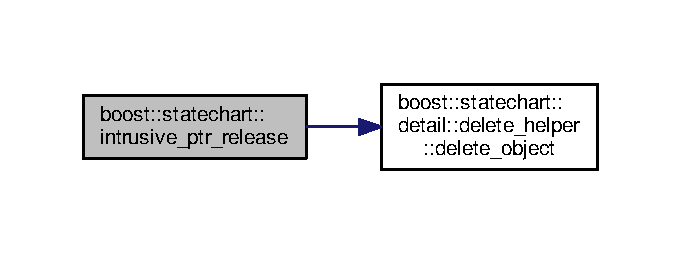
\includegraphics[width=327pt]{namespaceboost_1_1statechart_a1920a5b283c13c30ecd4aeb5b9499aeb_cgraph}
\end{center}
\end{figure}
\mbox{\Hypertarget{namespaceboost_1_1statechart_a16a84edc3e19176233fbdf977c1aa7ec}\label{namespaceboost_1_1statechart_a16a84edc3e19176233fbdf977c1aa7ec}} 
\index{boost\+::statechart@{boost\+::statechart}!intrusive\+\_\+ptr\+\_\+release@{intrusive\+\_\+ptr\+\_\+release}}
\index{intrusive\+\_\+ptr\+\_\+release@{intrusive\+\_\+ptr\+\_\+release}!boost\+::statechart@{boost\+::statechart}}
\subsubsection{\texorpdfstring{intrusive\+\_\+ptr\+\_\+release()}{intrusive\_ptr\_release()}\hspace{0.1cm}{\footnotesize\ttfamily [2/2]}}
{\footnotesize\ttfamily template$<$class Most\+Derived , class Context , class Inner\+Initial , history\+\_\+mode history\+Mode$>$ \\
void boost\+::statechart\+::intrusive\+\_\+ptr\+\_\+release (\begin{DoxyParamCaption}\item[{const \+::\mbox{\hyperlink{classboost_1_1statechart_1_1simple__state}{boost\+::statechart\+::simple\+\_\+state}}$<$ Most\+Derived, Context, Inner\+Initial, history\+Mode $>$ $\ast$}]{p\+Base }\end{DoxyParamCaption})\hspace{0.3cm}{\ttfamily [inline]}}


\hypertarget{namespaceboost_1_1statechart_1_1detail}{}\section{boost\+:\+:statechart\+:\+:detail Namespace Reference}
\label{namespaceboost_1_1statechart_1_1detail}\index{boost\+::statechart\+::detail@{boost\+::statechart\+::detail}}
\subsection*{Classes}
\begin{DoxyCompactItemize}
\item 
struct \mbox{\hyperlink{structboost_1_1statechart_1_1detail_1_1constructor}{constructor}}
\item 
struct \mbox{\hyperlink{structboost_1_1statechart_1_1detail_1_1constructor__impl}{constructor\+\_\+impl}}
\item 
struct \mbox{\hyperlink{structboost_1_1statechart_1_1detail_1_1count__base}{count\+\_\+base}}
\item 
struct \mbox{\hyperlink{structboost_1_1statechart_1_1detail_1_1count__base_3_01false_01_4}{count\+\_\+base$<$ false $>$}}
\item 
class \mbox{\hyperlink{classboost_1_1statechart_1_1detail_1_1counted__base}{counted\+\_\+base}}
\item 
struct \mbox{\hyperlink{structboost_1_1statechart_1_1detail_1_1deep__history__storer}{deep\+\_\+history\+\_\+storer}}
\item 
struct \mbox{\hyperlink{structboost_1_1statechart_1_1detail_1_1deep__history__storer_3_01true_00_01false_01_4}{deep\+\_\+history\+\_\+storer$<$ true, false $>$}}
\item 
struct \mbox{\hyperlink{structboost_1_1statechart_1_1detail_1_1deep__history__storer_3_01true_00_01true_01_4}{deep\+\_\+history\+\_\+storer$<$ true, true $>$}}
\item 
class \mbox{\hyperlink{classboost_1_1statechart_1_1detail_1_1delete__helper}{delete\+\_\+helper}}
\item 
class \mbox{\hyperlink{classboost_1_1statechart_1_1detail_1_1history__key}{history\+\_\+key}}
\item 
struct \mbox{\hyperlink{structboost_1_1statechart_1_1detail_1_1id__holder}{id\+\_\+holder}}
\item 
struct \mbox{\hyperlink{structboost_1_1statechart_1_1detail_1_1id__provider}{id\+\_\+provider}}
\item 
struct \mbox{\hyperlink{structboost_1_1statechart_1_1detail_1_1inner__constructor}{inner\+\_\+constructor}}
\item 
class \mbox{\hyperlink{classboost_1_1statechart_1_1detail_1_1leaf__state}{leaf\+\_\+state}}
\item 
struct \mbox{\hyperlink{structboost_1_1statechart_1_1detail_1_1make__context__list}{make\+\_\+context\+\_\+list}}
\item 
struct \mbox{\hyperlink{structboost_1_1statechart_1_1detail_1_1make__list}{make\+\_\+list}}
\item 
struct \mbox{\hyperlink{structboost_1_1statechart_1_1detail_1_1no__context}{no\+\_\+context}}
\item 
struct \mbox{\hyperlink{structboost_1_1statechart_1_1detail_1_1no__transition__function}{no\+\_\+transition\+\_\+function}}
\item 
class \mbox{\hyperlink{classboost_1_1statechart_1_1detail_1_1node__state}{node\+\_\+state}}
\item 
class \mbox{\hyperlink{classboost_1_1statechart_1_1detail_1_1node__state__base}{node\+\_\+state\+\_\+base}}
\item 
struct \mbox{\hyperlink{structboost_1_1statechart_1_1detail_1_1outer__constructor}{outer\+\_\+constructor}}
\item 
class \mbox{\hyperlink{classboost_1_1statechart_1_1detail_1_1reaction__dispatcher}{reaction\+\_\+dispatcher}}
\item 
struct \mbox{\hyperlink{structboost_1_1statechart_1_1detail_1_1result__utility}{result\+\_\+utility}}
\item 
struct \mbox{\hyperlink{structboost_1_1statechart_1_1detail_1_1rtti__policy}{rtti\+\_\+policy}}
\item 
class \mbox{\hyperlink{classboost_1_1statechart_1_1detail_1_1safe__reaction__result}{safe\+\_\+reaction\+\_\+result}}
\item 
class \mbox{\hyperlink{classboost_1_1statechart_1_1detail_1_1send__function}{send\+\_\+function}}
\item 
struct \mbox{\hyperlink{structboost_1_1statechart_1_1detail_1_1simple__state__base__type}{simple\+\_\+state\+\_\+base\+\_\+type}}
\item 
class \mbox{\hyperlink{classboost_1_1statechart_1_1detail_1_1state__base}{state\+\_\+base}}
\item 
struct \mbox{\hyperlink{structboost_1_1statechart_1_1detail_1_1state__cast__impl}{state\+\_\+cast\+\_\+impl}}
\item 
struct \mbox{\hyperlink{structboost_1_1statechart_1_1detail_1_1state__cast__impl__pointer__target}{state\+\_\+cast\+\_\+impl\+\_\+pointer\+\_\+target}}
\item 
struct \mbox{\hyperlink{structboost_1_1statechart_1_1detail_1_1state__cast__impl__reference__target}{state\+\_\+cast\+\_\+impl\+\_\+reference\+\_\+target}}
\item 
class \mbox{\hyperlink{classboost_1_1statechart_1_1detail_1_1transition__function}{transition\+\_\+function}}
\item 
struct \mbox{\hyperlink{structboost_1_1statechart_1_1detail_1_1unwrap}{unwrap}}
\item 
struct \mbox{\hyperlink{structboost_1_1statechart_1_1detail_1_1unwrap__impl}{unwrap\+\_\+impl}}
\item 
struct \mbox{\hyperlink{structboost_1_1statechart_1_1detail_1_1unwrap__impl_3_01true_01_4}{unwrap\+\_\+impl$<$ true $>$}}
\end{DoxyCompactItemize}
\subsection*{Typedefs}
\begin{DoxyCompactItemize}
\item 
typedef unsigned char \mbox{\hyperlink{namespaceboost_1_1statechart_1_1detail_a3bedea0b807a16fa222733417183d2c9}{orthogonal\+\_\+position\+\_\+type}}
\end{DoxyCompactItemize}
\subsection*{Enumerations}
\begin{DoxyCompactItemize}
\item 
enum \mbox{\hyperlink{namespaceboost_1_1statechart_1_1detail_ab091bbb4c29327fb46ee479ea1b7255b}{reaction\+\_\+result}} \{ \newline
\mbox{\hyperlink{namespaceboost_1_1statechart_1_1detail_ab091bbb4c29327fb46ee479ea1b7255ba4d86205de715a9babe60227df2fd0d13}{no\+\_\+reaction}}, 
\mbox{\hyperlink{namespaceboost_1_1statechart_1_1detail_ab091bbb4c29327fb46ee479ea1b7255ba4df2d08ea5b8ab72baf5ca9a98eaa8df}{do\+\_\+forward\+\_\+event}}, 
\mbox{\hyperlink{namespaceboost_1_1statechart_1_1detail_ab091bbb4c29327fb46ee479ea1b7255badd0f566df1a7b78d7db8c72fbfcb00a3}{do\+\_\+discard\+\_\+event}}, 
\mbox{\hyperlink{namespaceboost_1_1statechart_1_1detail_ab091bbb4c29327fb46ee479ea1b7255bae217591a2ca5982361b667f3a7865f95}{do\+\_\+defer\+\_\+event}}, 
\newline
\mbox{\hyperlink{namespaceboost_1_1statechart_1_1detail_ab091bbb4c29327fb46ee479ea1b7255bac26ab9d8d80f4ebadd553d4c8ee851c8}{consumed}}
 \}
\end{DoxyCompactItemize}
\subsection*{Functions}
\begin{DoxyCompactItemize}
\item 
{\footnotesize template$<$typename T $>$ }\\void \mbox{\hyperlink{namespaceboost_1_1statechart_1_1detail_a4c8f28e86a5c5c087b5a1b2e546cc93b}{avoid\+\_\+unused\+\_\+warning}} (const T \&)
\item 
{\footnotesize template$<$class Most\+Derived , class Allocator $>$ }\\void $\ast$ \mbox{\hyperlink{namespaceboost_1_1statechart_1_1detail_a23e46110b9423928f648c10933316959}{allocate}} (std\+::size\+\_\+t size)
\item 
{\footnotesize template$<$class Most\+Derived , class Allocator $>$ }\\void \mbox{\hyperlink{namespaceboost_1_1statechart_1_1detail_a2137e00f346972cc349b4eb44a806213}{deallocate}} (void $\ast$p\+Object)
\item 
{\footnotesize template$<$class Allocator , class Rtti\+Policy $>$ }\\void \mbox{\hyperlink{namespaceboost_1_1statechart_1_1detail_ae61199991db81ca38c21e4b657993be5}{intrusive\+\_\+ptr\+\_\+add\+\_\+ref}} (const \+::\mbox{\hyperlink{classboost_1_1statechart_1_1detail_1_1state__base}{boost\+::statechart\+::detail\+::state\+\_\+base}}$<$ Allocator, Rtti\+Policy $>$ $\ast$p\+Base)
\item 
{\footnotesize template$<$class Allocator , class Rtti\+Policy $>$ }\\void \mbox{\hyperlink{namespaceboost_1_1statechart_1_1detail_a783126c1ee44ec8984ee4d89b0aa1eac}{intrusive\+\_\+ptr\+\_\+release}} (const \+::\mbox{\hyperlink{classboost_1_1statechart_1_1detail_1_1state__base}{boost\+::statechart\+::detail\+::state\+\_\+base}}$<$ Allocator, Rtti\+Policy $>$ $\ast$p\+Base)
\end{DoxyCompactItemize}


\subsection{Typedef Documentation}
\mbox{\Hypertarget{namespaceboost_1_1statechart_1_1detail_a3bedea0b807a16fa222733417183d2c9}\label{namespaceboost_1_1statechart_1_1detail_a3bedea0b807a16fa222733417183d2c9}} 
\index{boost\+::statechart\+::detail@{boost\+::statechart\+::detail}!orthogonal\+\_\+position\+\_\+type@{orthogonal\+\_\+position\+\_\+type}}
\index{orthogonal\+\_\+position\+\_\+type@{orthogonal\+\_\+position\+\_\+type}!boost\+::statechart\+::detail@{boost\+::statechart\+::detail}}
\subsubsection{\texorpdfstring{orthogonal\+\_\+position\+\_\+type}{orthogonal\_position\_type}}
{\footnotesize\ttfamily typedef unsigned char \mbox{\hyperlink{namespaceboost_1_1statechart_1_1detail_a3bedea0b807a16fa222733417183d2c9}{boost\+::statechart\+::detail\+::orthogonal\+\_\+position\+\_\+type}}}



\subsection{Enumeration Type Documentation}
\mbox{\Hypertarget{namespaceboost_1_1statechart_1_1detail_ab091bbb4c29327fb46ee479ea1b7255b}\label{namespaceboost_1_1statechart_1_1detail_ab091bbb4c29327fb46ee479ea1b7255b}} 
\index{boost\+::statechart\+::detail@{boost\+::statechart\+::detail}!reaction\+\_\+result@{reaction\+\_\+result}}
\index{reaction\+\_\+result@{reaction\+\_\+result}!boost\+::statechart\+::detail@{boost\+::statechart\+::detail}}
\subsubsection{\texorpdfstring{reaction\+\_\+result}{reaction\_result}}
{\footnotesize\ttfamily enum \mbox{\hyperlink{namespaceboost_1_1statechart_1_1detail_ab091bbb4c29327fb46ee479ea1b7255b}{boost\+::statechart\+::detail\+::reaction\+\_\+result}}}

\begin{DoxyEnumFields}{Enumerator}
\raisebox{\heightof{T}}[0pt][0pt]{\index{no\+\_\+reaction@{no\+\_\+reaction}!boost\+::statechart\+::detail@{boost\+::statechart\+::detail}}\index{boost\+::statechart\+::detail@{boost\+::statechart\+::detail}!no\+\_\+reaction@{no\+\_\+reaction}}}\mbox{\Hypertarget{namespaceboost_1_1statechart_1_1detail_ab091bbb4c29327fb46ee479ea1b7255ba4d86205de715a9babe60227df2fd0d13}\label{namespaceboost_1_1statechart_1_1detail_ab091bbb4c29327fb46ee479ea1b7255ba4d86205de715a9babe60227df2fd0d13}} 
no\+\_\+reaction&\\
\hline

\raisebox{\heightof{T}}[0pt][0pt]{\index{do\+\_\+forward\+\_\+event@{do\+\_\+forward\+\_\+event}!boost\+::statechart\+::detail@{boost\+::statechart\+::detail}}\index{boost\+::statechart\+::detail@{boost\+::statechart\+::detail}!do\+\_\+forward\+\_\+event@{do\+\_\+forward\+\_\+event}}}\mbox{\Hypertarget{namespaceboost_1_1statechart_1_1detail_ab091bbb4c29327fb46ee479ea1b7255ba4df2d08ea5b8ab72baf5ca9a98eaa8df}\label{namespaceboost_1_1statechart_1_1detail_ab091bbb4c29327fb46ee479ea1b7255ba4df2d08ea5b8ab72baf5ca9a98eaa8df}} 
do\+\_\+forward\+\_\+event&\\
\hline

\raisebox{\heightof{T}}[0pt][0pt]{\index{do\+\_\+discard\+\_\+event@{do\+\_\+discard\+\_\+event}!boost\+::statechart\+::detail@{boost\+::statechart\+::detail}}\index{boost\+::statechart\+::detail@{boost\+::statechart\+::detail}!do\+\_\+discard\+\_\+event@{do\+\_\+discard\+\_\+event}}}\mbox{\Hypertarget{namespaceboost_1_1statechart_1_1detail_ab091bbb4c29327fb46ee479ea1b7255badd0f566df1a7b78d7db8c72fbfcb00a3}\label{namespaceboost_1_1statechart_1_1detail_ab091bbb4c29327fb46ee479ea1b7255badd0f566df1a7b78d7db8c72fbfcb00a3}} 
do\+\_\+discard\+\_\+event&\\
\hline

\raisebox{\heightof{T}}[0pt][0pt]{\index{do\+\_\+defer\+\_\+event@{do\+\_\+defer\+\_\+event}!boost\+::statechart\+::detail@{boost\+::statechart\+::detail}}\index{boost\+::statechart\+::detail@{boost\+::statechart\+::detail}!do\+\_\+defer\+\_\+event@{do\+\_\+defer\+\_\+event}}}\mbox{\Hypertarget{namespaceboost_1_1statechart_1_1detail_ab091bbb4c29327fb46ee479ea1b7255bae217591a2ca5982361b667f3a7865f95}\label{namespaceboost_1_1statechart_1_1detail_ab091bbb4c29327fb46ee479ea1b7255bae217591a2ca5982361b667f3a7865f95}} 
do\+\_\+defer\+\_\+event&\\
\hline

\raisebox{\heightof{T}}[0pt][0pt]{\index{consumed@{consumed}!boost\+::statechart\+::detail@{boost\+::statechart\+::detail}}\index{boost\+::statechart\+::detail@{boost\+::statechart\+::detail}!consumed@{consumed}}}\mbox{\Hypertarget{namespaceboost_1_1statechart_1_1detail_ab091bbb4c29327fb46ee479ea1b7255bac26ab9d8d80f4ebadd553d4c8ee851c8}\label{namespaceboost_1_1statechart_1_1detail_ab091bbb4c29327fb46ee479ea1b7255bac26ab9d8d80f4ebadd553d4c8ee851c8}} 
consumed&\\
\hline

\end{DoxyEnumFields}


\subsection{Function Documentation}
\mbox{\Hypertarget{namespaceboost_1_1statechart_1_1detail_a23e46110b9423928f648c10933316959}\label{namespaceboost_1_1statechart_1_1detail_a23e46110b9423928f648c10933316959}} 
\index{boost\+::statechart\+::detail@{boost\+::statechart\+::detail}!allocate@{allocate}}
\index{allocate@{allocate}!boost\+::statechart\+::detail@{boost\+::statechart\+::detail}}
\subsubsection{\texorpdfstring{allocate()}{allocate()}}
{\footnotesize\ttfamily template$<$class Most\+Derived , class Allocator $>$ \\
void$\ast$ boost\+::statechart\+::detail\+::allocate (\begin{DoxyParamCaption}\item[{std\+::size\+\_\+t}]{size }\end{DoxyParamCaption})}

Here is the call graph for this function\+:
\nopagebreak
\begin{figure}[H]
\begin{center}
\leavevmode
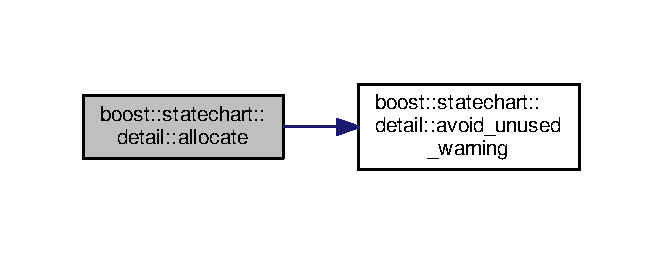
\includegraphics[width=318pt]{namespaceboost_1_1statechart_1_1detail_a23e46110b9423928f648c10933316959_cgraph}
\end{center}
\end{figure}
Here is the caller graph for this function\+:
\nopagebreak
\begin{figure}[H]
\begin{center}
\leavevmode
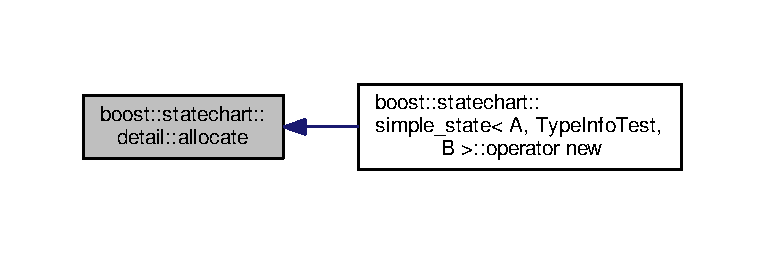
\includegraphics[width=350pt]{namespaceboost_1_1statechart_1_1detail_a23e46110b9423928f648c10933316959_icgraph}
\end{center}
\end{figure}
\mbox{\Hypertarget{namespaceboost_1_1statechart_1_1detail_a4c8f28e86a5c5c087b5a1b2e546cc93b}\label{namespaceboost_1_1statechart_1_1detail_a4c8f28e86a5c5c087b5a1b2e546cc93b}} 
\index{boost\+::statechart\+::detail@{boost\+::statechart\+::detail}!avoid\+\_\+unused\+\_\+warning@{avoid\+\_\+unused\+\_\+warning}}
\index{avoid\+\_\+unused\+\_\+warning@{avoid\+\_\+unused\+\_\+warning}!boost\+::statechart\+::detail@{boost\+::statechart\+::detail}}
\subsubsection{\texorpdfstring{avoid\+\_\+unused\+\_\+warning()}{avoid\_unused\_warning()}}
{\footnotesize\ttfamily template$<$typename T $>$ \\
void boost\+::statechart\+::detail\+::avoid\+\_\+unused\+\_\+warning (\begin{DoxyParamCaption}\item[{const T \&}]{ }\end{DoxyParamCaption})\hspace{0.3cm}{\ttfamily [inline]}}

Here is the caller graph for this function\+:
\nopagebreak
\begin{figure}[H]
\begin{center}
\leavevmode
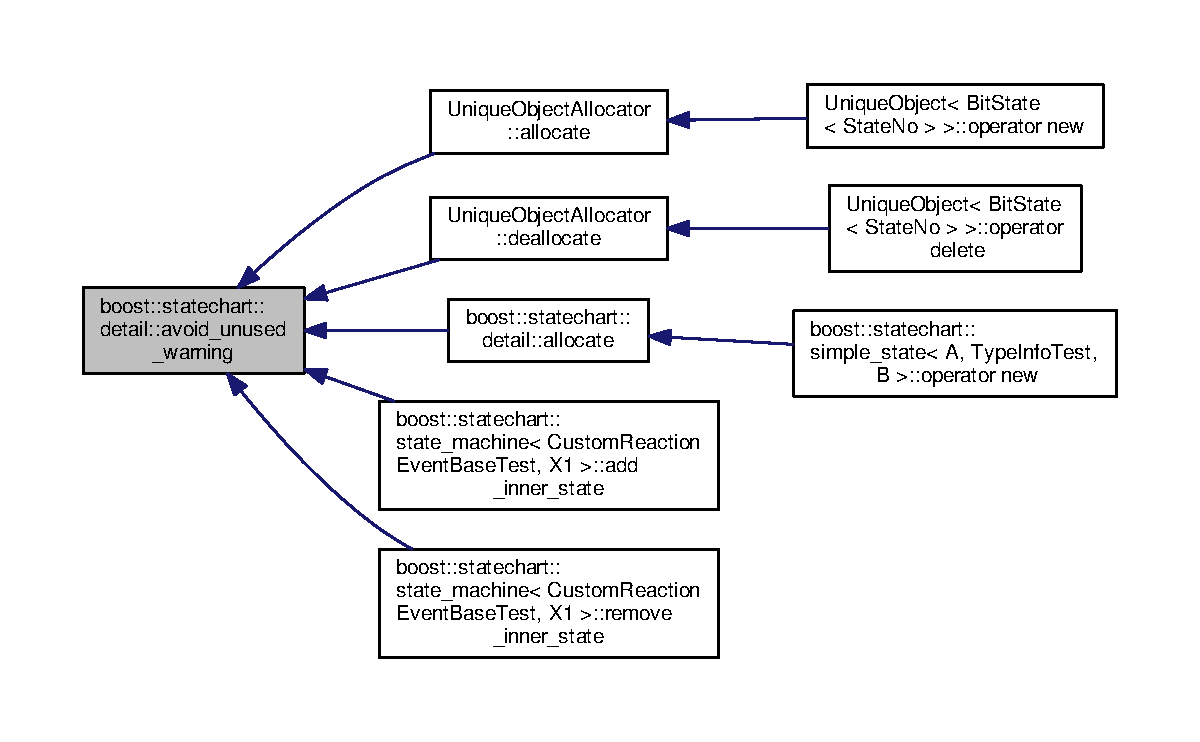
\includegraphics[width=350pt]{namespaceboost_1_1statechart_1_1detail_a4c8f28e86a5c5c087b5a1b2e546cc93b_icgraph}
\end{center}
\end{figure}
\mbox{\Hypertarget{namespaceboost_1_1statechart_1_1detail_a2137e00f346972cc349b4eb44a806213}\label{namespaceboost_1_1statechart_1_1detail_a2137e00f346972cc349b4eb44a806213}} 
\index{boost\+::statechart\+::detail@{boost\+::statechart\+::detail}!deallocate@{deallocate}}
\index{deallocate@{deallocate}!boost\+::statechart\+::detail@{boost\+::statechart\+::detail}}
\subsubsection{\texorpdfstring{deallocate()}{deallocate()}}
{\footnotesize\ttfamily template$<$class Most\+Derived , class Allocator $>$ \\
void boost\+::statechart\+::detail\+::deallocate (\begin{DoxyParamCaption}\item[{void $\ast$}]{p\+Object }\end{DoxyParamCaption})}

Here is the caller graph for this function\+:
\nopagebreak
\begin{figure}[H]
\begin{center}
\leavevmode
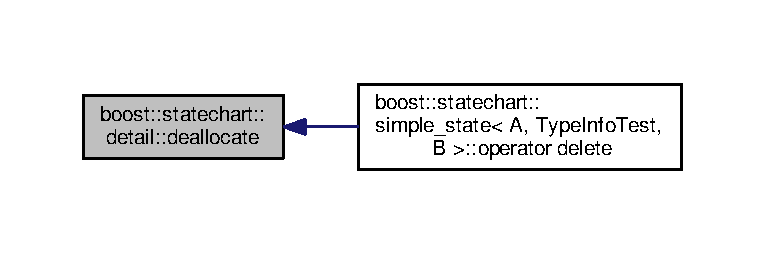
\includegraphics[width=350pt]{namespaceboost_1_1statechart_1_1detail_a2137e00f346972cc349b4eb44a806213_icgraph}
\end{center}
\end{figure}
\mbox{\Hypertarget{namespaceboost_1_1statechart_1_1detail_ae61199991db81ca38c21e4b657993be5}\label{namespaceboost_1_1statechart_1_1detail_ae61199991db81ca38c21e4b657993be5}} 
\index{boost\+::statechart\+::detail@{boost\+::statechart\+::detail}!intrusive\+\_\+ptr\+\_\+add\+\_\+ref@{intrusive\+\_\+ptr\+\_\+add\+\_\+ref}}
\index{intrusive\+\_\+ptr\+\_\+add\+\_\+ref@{intrusive\+\_\+ptr\+\_\+add\+\_\+ref}!boost\+::statechart\+::detail@{boost\+::statechart\+::detail}}
\subsubsection{\texorpdfstring{intrusive\+\_\+ptr\+\_\+add\+\_\+ref()}{intrusive\_ptr\_add\_ref()}}
{\footnotesize\ttfamily template$<$class Allocator , class Rtti\+Policy $>$ \\
void boost\+::statechart\+::detail\+::intrusive\+\_\+ptr\+\_\+add\+\_\+ref (\begin{DoxyParamCaption}\item[{const \+::\mbox{\hyperlink{classboost_1_1statechart_1_1detail_1_1state__base}{boost\+::statechart\+::detail\+::state\+\_\+base}}$<$ Allocator, Rtti\+Policy $>$ $\ast$}]{p\+Base }\end{DoxyParamCaption})\hspace{0.3cm}{\ttfamily [inline]}}

\mbox{\Hypertarget{namespaceboost_1_1statechart_1_1detail_a783126c1ee44ec8984ee4d89b0aa1eac}\label{namespaceboost_1_1statechart_1_1detail_a783126c1ee44ec8984ee4d89b0aa1eac}} 
\index{boost\+::statechart\+::detail@{boost\+::statechart\+::detail}!intrusive\+\_\+ptr\+\_\+release@{intrusive\+\_\+ptr\+\_\+release}}
\index{intrusive\+\_\+ptr\+\_\+release@{intrusive\+\_\+ptr\+\_\+release}!boost\+::statechart\+::detail@{boost\+::statechart\+::detail}}
\subsubsection{\texorpdfstring{intrusive\+\_\+ptr\+\_\+release()}{intrusive\_ptr\_release()}}
{\footnotesize\ttfamily template$<$class Allocator , class Rtti\+Policy $>$ \\
void boost\+::statechart\+::detail\+::intrusive\+\_\+ptr\+\_\+release (\begin{DoxyParamCaption}\item[{const \+::\mbox{\hyperlink{classboost_1_1statechart_1_1detail_1_1state__base}{boost\+::statechart\+::detail\+::state\+\_\+base}}$<$ Allocator, Rtti\+Policy $>$ $\ast$}]{p\+Base }\end{DoxyParamCaption})\hspace{0.3cm}{\ttfamily [inline]}}


\chapter{Class Documentation}
\hypertarget{struct_a}{}\section{A Struct Reference}
\label{struct_a}\index{A@{A}}


Inheritance diagram for A\+:
\nopagebreak
\begin{figure}[H]
\begin{center}
\leavevmode
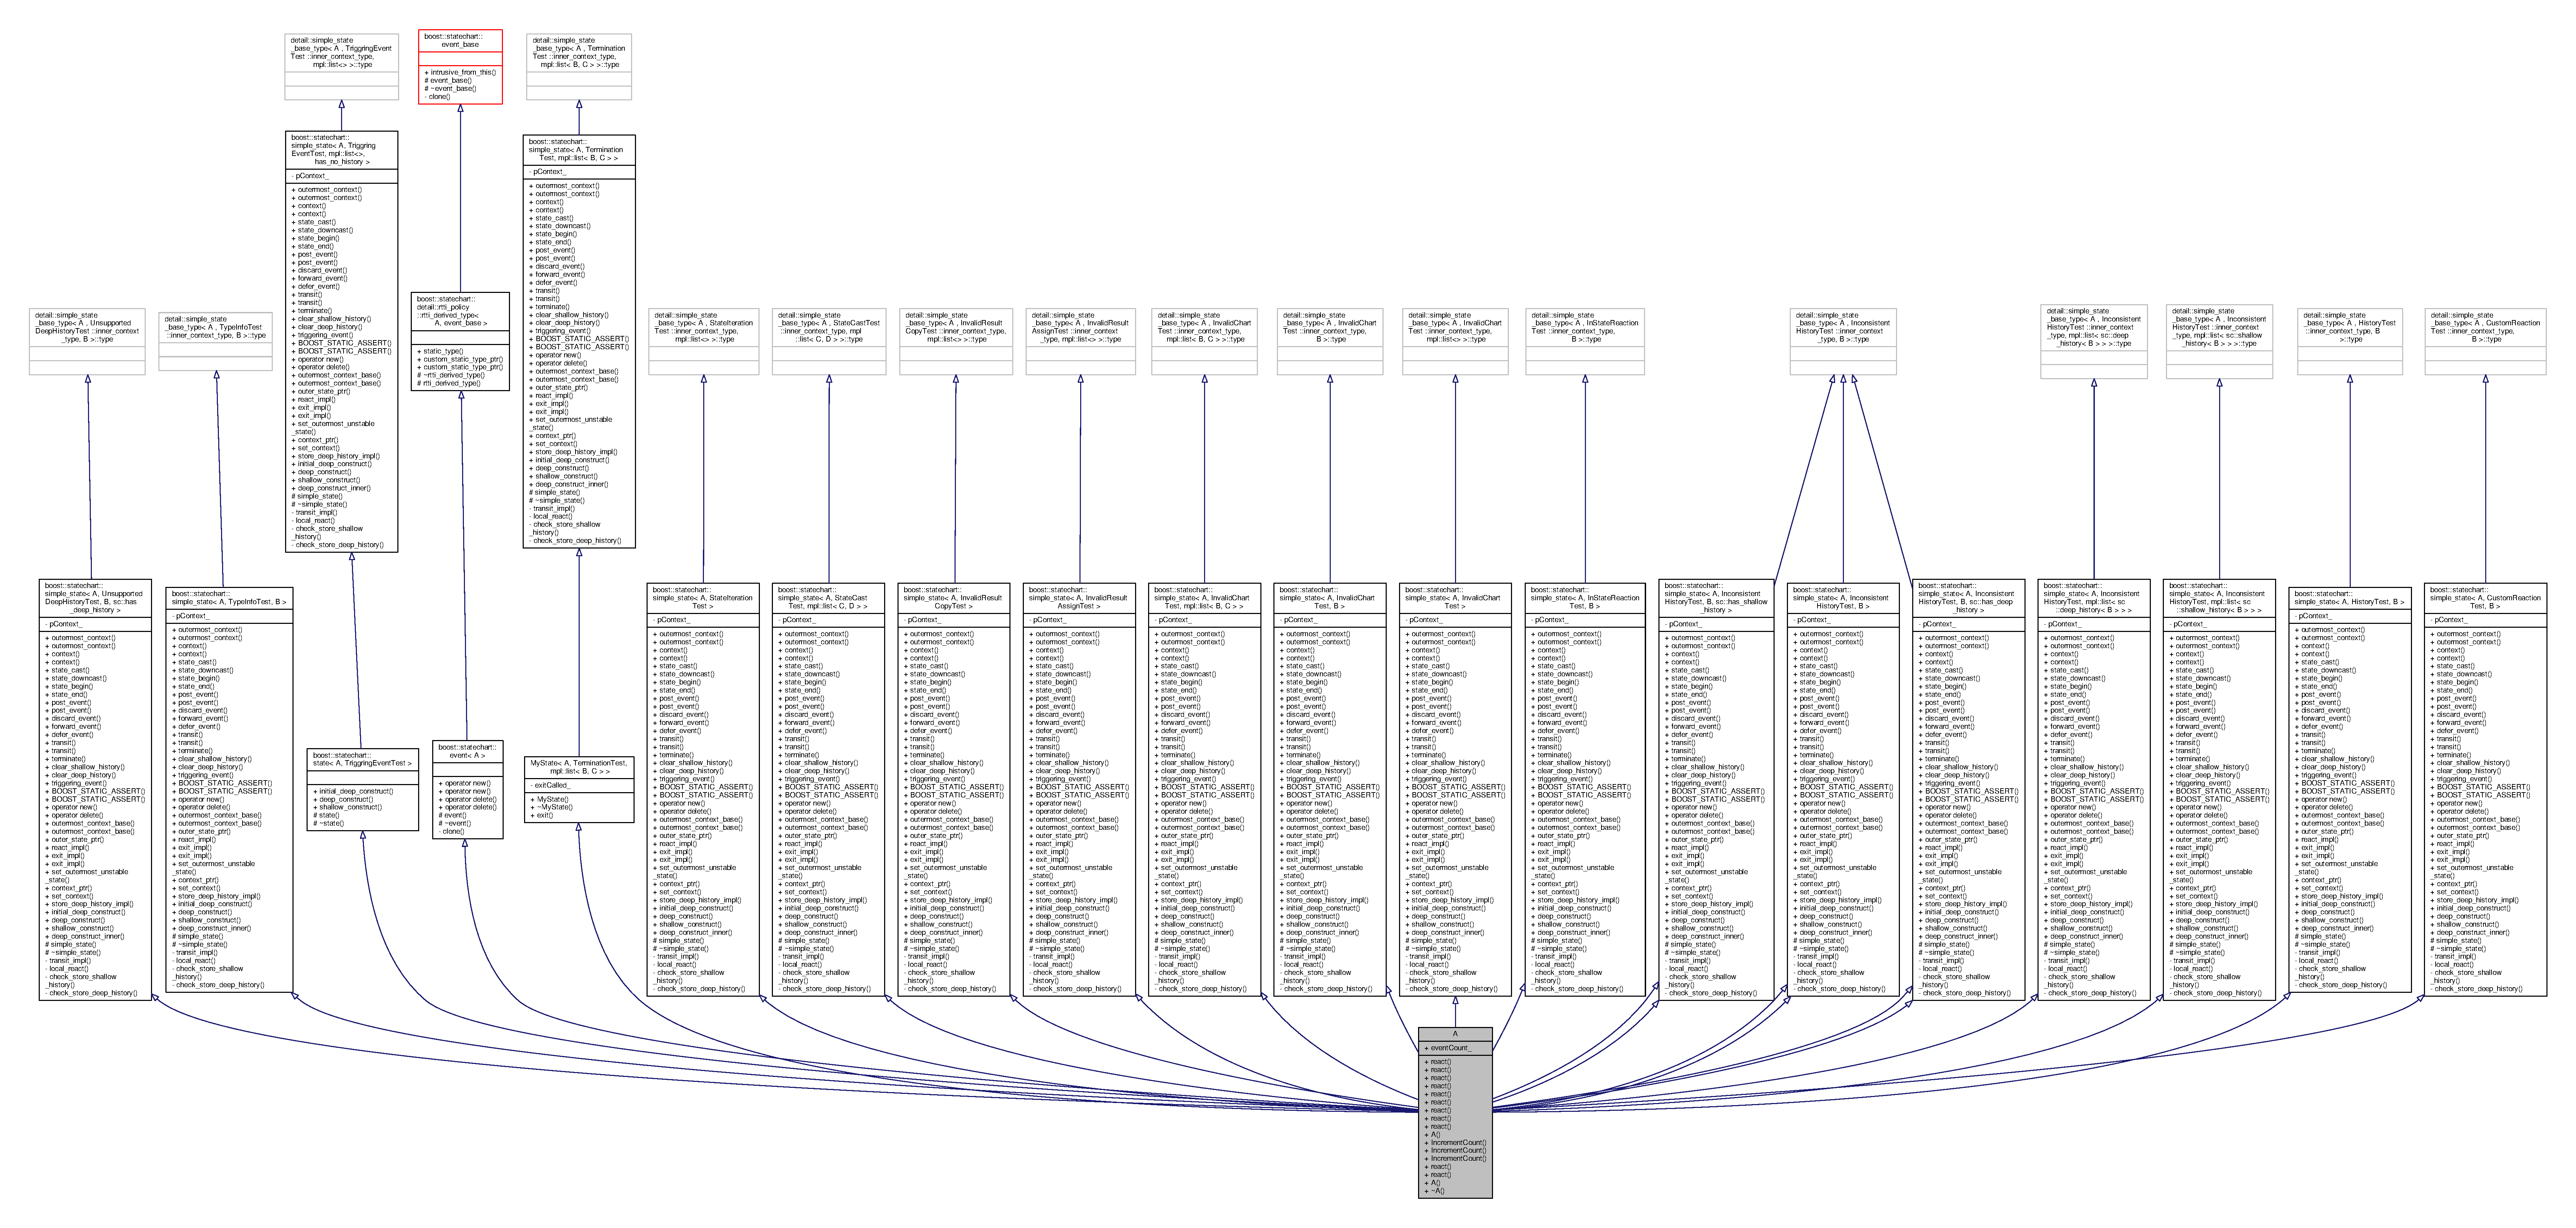
\includegraphics[width=350pt]{struct_a__inherit__graph}
\end{center}
\end{figure}


Collaboration diagram for A\+:
\nopagebreak
\begin{figure}[H]
\begin{center}
\leavevmode
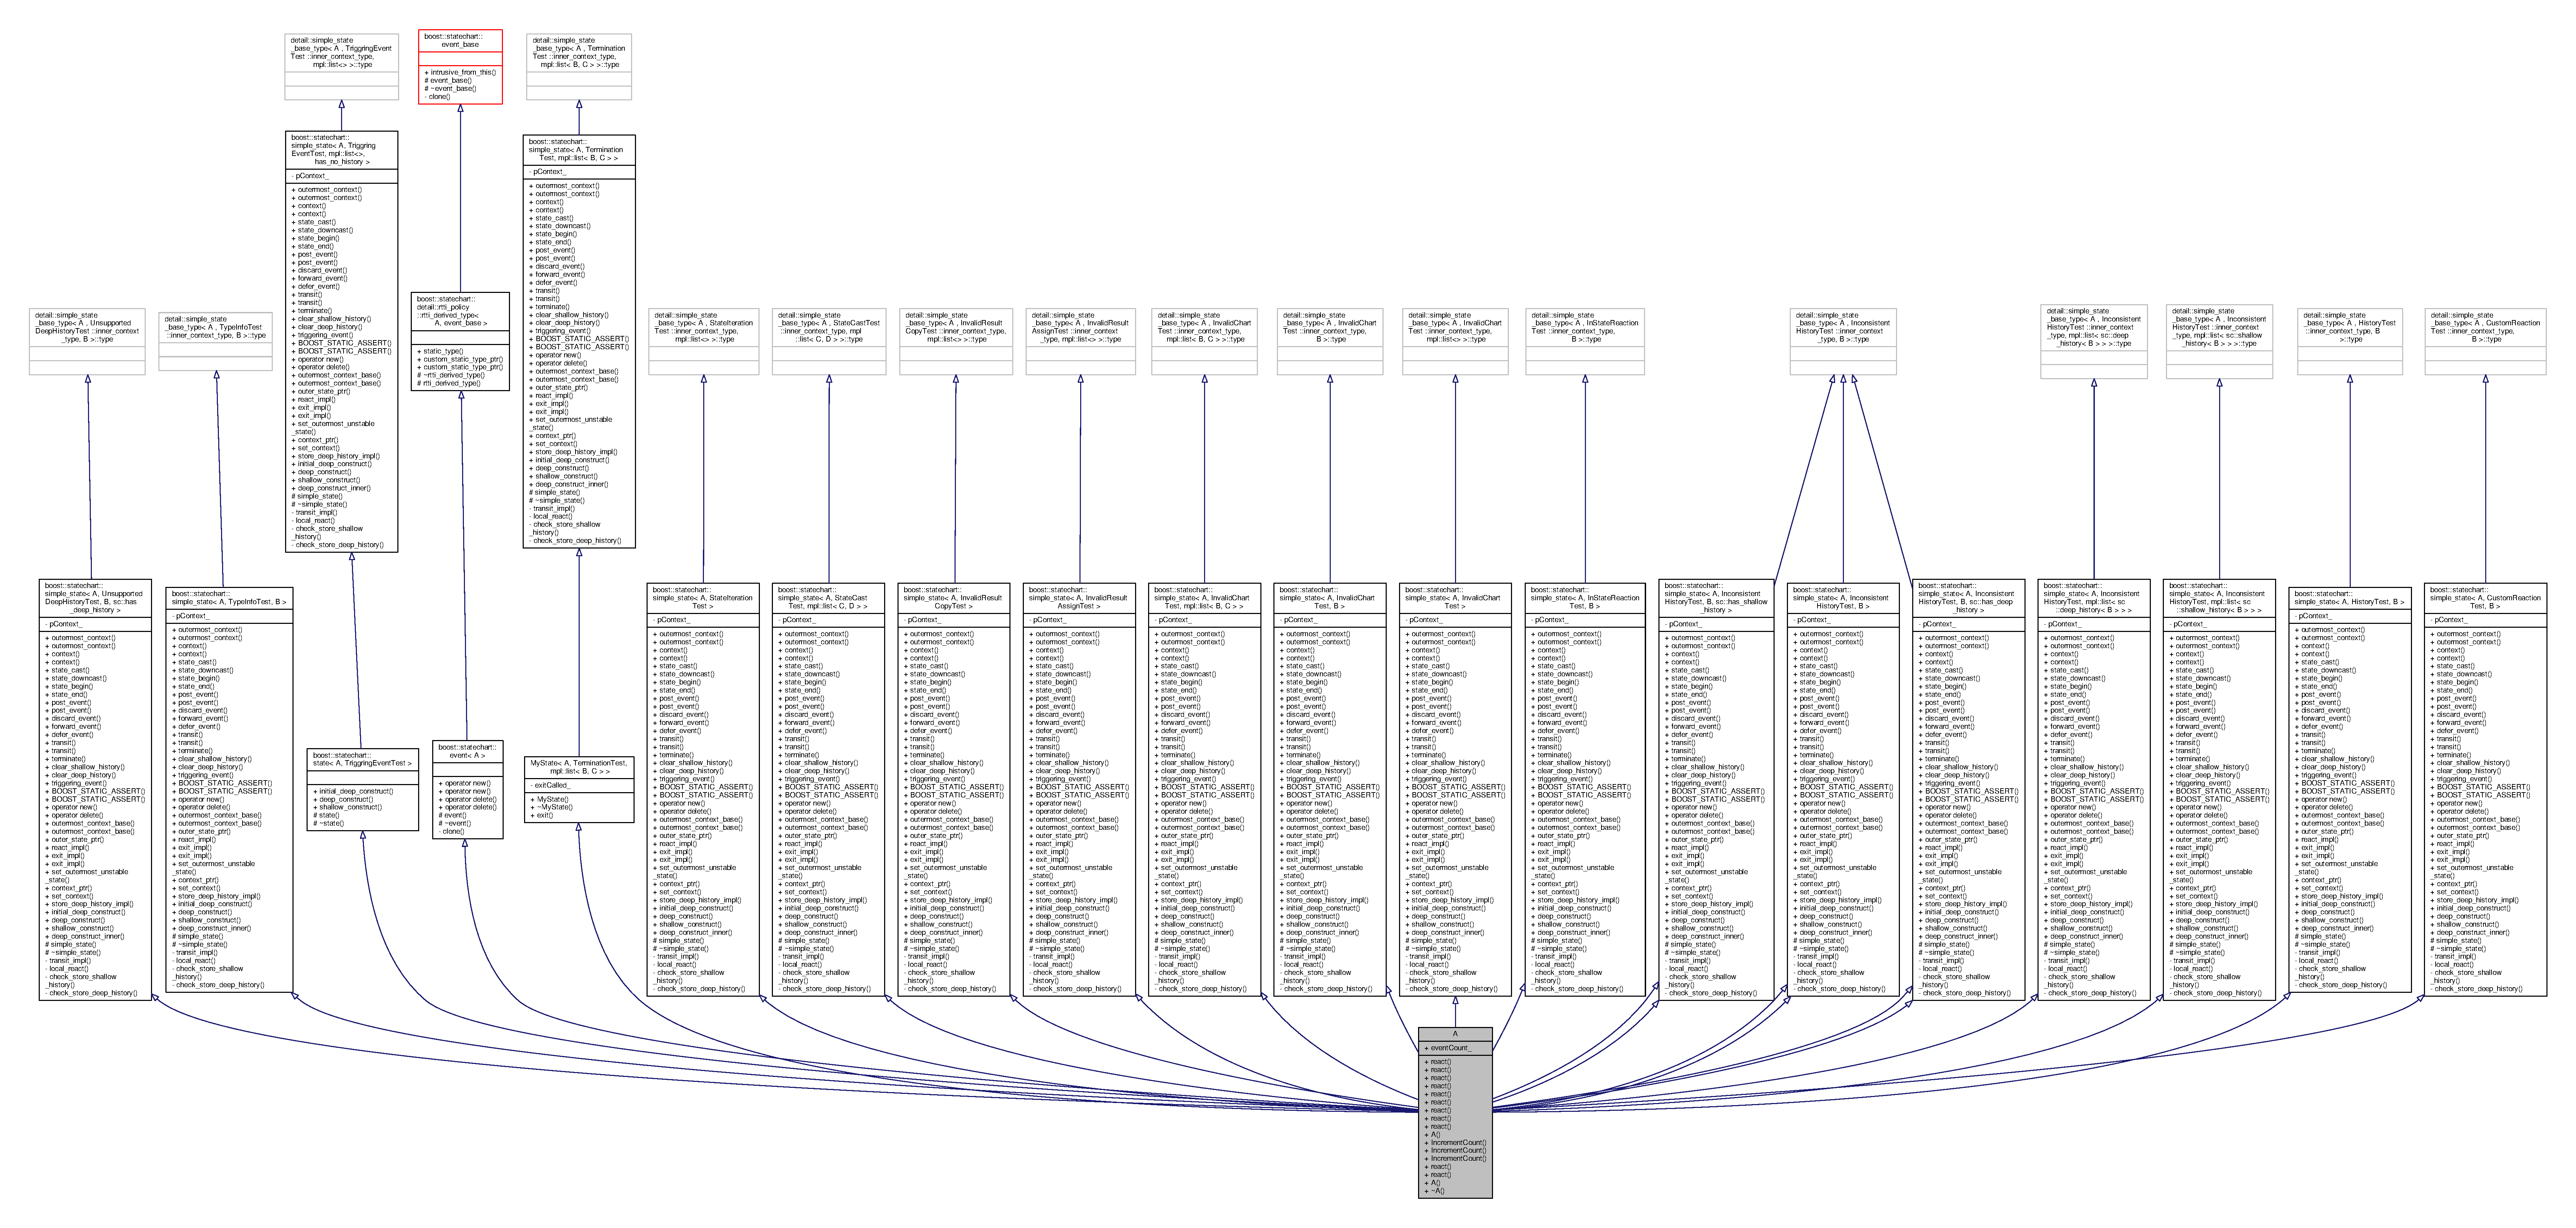
\includegraphics[width=350pt]{struct_a__coll__graph}
\end{center}
\end{figure}
\subsection*{Public Types}
\begin{DoxyCompactItemize}
\item 
typedef mpl\+::list$<$ \mbox{\hyperlink{classboost_1_1statechart_1_1custom__reaction}{sc\+::custom\+\_\+reaction}}$<$ \mbox{\hyperlink{struct_ev_discard_never}{Ev\+Discard\+Never}} $>$, \mbox{\hyperlink{classboost_1_1statechart_1_1custom__reaction}{sc\+::custom\+\_\+reaction}}$<$ \mbox{\hyperlink{struct_ev_discard_in_b}{Ev\+Discard\+InB}} $>$, \mbox{\hyperlink{classboost_1_1statechart_1_1custom__reaction}{sc\+::custom\+\_\+reaction}}$<$ \mbox{\hyperlink{struct_ev_discard_in_d}{Ev\+Discard\+InD}} $>$, \mbox{\hyperlink{classboost_1_1statechart_1_1custom__reaction}{sc\+::custom\+\_\+reaction}}$<$ \mbox{\hyperlink{struct_ev_defer}{Ev\+Defer}} $>$, \mbox{\hyperlink{classboost_1_1statechart_1_1custom__reaction}{sc\+::custom\+\_\+reaction}}$<$ \mbox{\hyperlink{struct_ev_terminate}{Ev\+Terminate}} $>$, \mbox{\hyperlink{classboost_1_1statechart_1_1custom__reaction}{sc\+::custom\+\_\+reaction}}$<$ \mbox{\hyperlink{struct_ev_transit_with_action}{Ev\+Transit\+With\+Action}} $>$, \mbox{\hyperlink{classboost_1_1statechart_1_1custom__reaction}{sc\+::custom\+\_\+reaction}}$<$ \mbox{\hyperlink{struct_ev_transit}{Ev\+Transit}} $>$ $>$ \mbox{\hyperlink{struct_a_aaf7ef039e669b21e19f81777afeed659}{reactions}}
\item 
typedef mpl\+::list$<$ \mbox{\hyperlink{classboost_1_1statechart_1_1transition}{sc\+::transition}}$<$ \mbox{\hyperlink{struct_ev_to_b}{Ev\+ToB}}, \mbox{\hyperlink{struct_b}{B}} $>$, \mbox{\hyperlink{classboost_1_1statechart_1_1transition}{sc\+::transition}}$<$ \mbox{\hyperlink{struct_ev_to_d}{Ev\+ToD}}, \mbox{\hyperlink{struct_d}{D}} $>$, \mbox{\hyperlink{classboost_1_1statechart_1_1transition}{sc\+::transition}}$<$ \mbox{\hyperlink{struct_ev_to_d_shallow}{Ev\+To\+D\+Shallow}}, \mbox{\hyperlink{classboost_1_1statechart_1_1shallow__history}{sc\+::shallow\+\_\+history}}$<$ \mbox{\hyperlink{struct_d}{D}} $>$ $>$, \mbox{\hyperlink{classboost_1_1statechart_1_1transition}{sc\+::transition}}$<$ \mbox{\hyperlink{struct_ev_to_d_deep}{Ev\+To\+D\+Deep}}, \mbox{\hyperlink{classboost_1_1statechart_1_1deep__history}{sc\+::deep\+\_\+history}}$<$ \mbox{\hyperlink{struct_d}{D}} $>$ $>$, \mbox{\hyperlink{classboost_1_1statechart_1_1transition}{sc\+::transition}}$<$ \mbox{\hyperlink{struct_ev_to_f}{Ev\+ToF}}, \mbox{\hyperlink{struct_f}{F}} $>$, \mbox{\hyperlink{classboost_1_1statechart_1_1transition}{sc\+::transition}}$<$ \mbox{\hyperlink{struct_ev_to_f_shallow}{Ev\+To\+F\+Shallow}}, \mbox{\hyperlink{classboost_1_1statechart_1_1shallow__history}{sc\+::shallow\+\_\+history}}$<$ \mbox{\hyperlink{struct_f}{F}} $>$ $>$, \mbox{\hyperlink{classboost_1_1statechart_1_1transition}{sc\+::transition}}$<$ \mbox{\hyperlink{struct_ev_to_f_deep}{Ev\+To\+F\+Deep}}, \mbox{\hyperlink{classboost_1_1statechart_1_1deep__history}{sc\+::deep\+\_\+history}}$<$ \mbox{\hyperlink{struct_f}{F}} $>$ $>$, \mbox{\hyperlink{classboost_1_1statechart_1_1transition}{sc\+::transition}}$<$ \mbox{\hyperlink{struct_ev_to_h}{Ev\+ToH}}, \mbox{\hyperlink{struct_h}{H}} $>$, \mbox{\hyperlink{classboost_1_1statechart_1_1transition}{sc\+::transition}}$<$ \mbox{\hyperlink{struct_ev_to_i}{Ev\+ToI}}, \mbox{\hyperlink{struct_i}{I}} $>$, \mbox{\hyperlink{classboost_1_1statechart_1_1transition}{sc\+::transition}}$<$ \mbox{\hyperlink{struct_ev_to_m}{Ev\+ToM}}, \mbox{\hyperlink{struct_m}{M}} $>$, \mbox{\hyperlink{classboost_1_1statechart_1_1transition}{sc\+::transition}}$<$ \mbox{\hyperlink{struct_ev_to_q}{Ev\+ToQ}}, \mbox{\hyperlink{struct_q}{Q}} $>$ $>$ \mbox{\hyperlink{struct_a_acf0421a3801f117c8a6d59698bdb3f40}{reactions}}
\item 
typedef \mbox{\hyperlink{classboost_1_1statechart_1_1transition}{sc\+::transition}}$<$ \mbox{\hyperlink{struct_ev_x}{EvX}}, \mbox{\hyperlink{classboost_1_1statechart_1_1shallow__history}{sc\+::shallow\+\_\+history}}$<$ \mbox{\hyperlink{struct_b}{B}} $>$ $>$ \mbox{\hyperlink{struct_a_aaea4dcd074640c12d239e2c4fd846adc}{reactions}}
\item 
typedef \mbox{\hyperlink{classboost_1_1statechart_1_1transition}{sc\+::transition}}$<$ \mbox{\hyperlink{struct_ev_x}{EvX}}, \mbox{\hyperlink{classboost_1_1statechart_1_1deep__history}{sc\+::deep\+\_\+history}}$<$ \mbox{\hyperlink{struct_b}{B}} $>$ $>$ \mbox{\hyperlink{struct_a_a336e15662d0cfb81d1abb41df9fca187}{reactions}}
\item 
typedef \mbox{\hyperlink{classboost_1_1statechart_1_1custom__reaction}{sc\+::custom\+\_\+reaction}}$<$ \mbox{\hyperlink{struct_ev_x}{EvX}} $>$ \mbox{\hyperlink{struct_a_aca29ac82093be1c88d8177f5108af763}{reactions}}
\item 
typedef \mbox{\hyperlink{classboost_1_1statechart_1_1custom__reaction}{sc\+::custom\+\_\+reaction}}$<$ \mbox{\hyperlink{struct_ev_x}{EvX}} $>$ \mbox{\hyperlink{struct_a_aca29ac82093be1c88d8177f5108af763}{reactions}}
\item 
typedef mpl\+::list$<$ \mbox{\hyperlink{classboost_1_1statechart_1_1in__state__reaction}{sc\+::in\+\_\+state\+\_\+reaction}}$<$ \mbox{\hyperlink{struct_e}{E}}, \mbox{\hyperlink{struct_a}{A}}, \&\mbox{\hyperlink{struct_a_a7811ed8883449fde0d5f59bd2ebf3de5}{A\+::\+Increment\+Count}} $>$, \mbox{\hyperlink{classboost_1_1statechart_1_1in__state__reaction}{sc\+::in\+\_\+state\+\_\+reaction}}$<$ \mbox{\hyperlink{classboost_1_1statechart_1_1event__base}{sc\+::event\+\_\+base}}, \mbox{\hyperlink{struct_a}{A}}, \&\mbox{\hyperlink{struct_a_a7811ed8883449fde0d5f59bd2ebf3de5}{A\+::\+Increment\+Count}} $>$ $>$ \mbox{\hyperlink{struct_a_a34d11f67d397f777186858587949c5a2}{reactions}}
\item 
typedef \mbox{\hyperlink{classboost_1_1statechart_1_1custom__reaction}{sc\+::custom\+\_\+reaction}}$<$ \mbox{\hyperlink{struct_e}{E}} $>$ \mbox{\hyperlink{struct_a_a34ec5dc41104a605ae13eff9a6a97a39}{reactions}}
\item 
typedef \mbox{\hyperlink{classboost_1_1statechart_1_1custom__reaction}{sc\+::custom\+\_\+reaction}}$<$ \mbox{\hyperlink{struct_e}{E}} $>$ \mbox{\hyperlink{struct_a_a34ec5dc41104a605ae13eff9a6a97a39}{reactions}}
\item 
typedef \mbox{\hyperlink{classboost_1_1statechart_1_1transition}{sc\+::transition}}$<$ \mbox{\hyperlink{struct_ev_to_b}{Ev\+ToB}}, \mbox{\hyperlink{struct_b}{B}} $>$ \mbox{\hyperlink{struct_a_a14567593462fe87eb5c35b1c564dc869}{reactions}}
\item 
typedef \mbox{\hyperlink{classboost_1_1statechart_1_1transition}{sc\+::transition}}$<$ \mbox{\hyperlink{struct_ev_to_b}{Ev\+ToB}}, \mbox{\hyperlink{struct_b}{B}} $>$ \mbox{\hyperlink{struct_a_a14567593462fe87eb5c35b1c564dc869}{reactions}}
\item 
typedef \mbox{\hyperlink{classboost_1_1statechart_1_1termination}{sc\+::termination}}$<$ \mbox{\hyperlink{struct_ev_terminate_a}{Ev\+TerminateA}} $>$ \mbox{\hyperlink{struct_a_a9fdfa49e1cf1fe54c74cab8e5e690f55}{reactions}}
\item 
typedef \mbox{\hyperlink{classboost_1_1statechart_1_1transition}{sc\+::transition}}$<$ \mbox{\hyperlink{struct_ev_go_to_b}{Ev\+Go\+ToB}}, \mbox{\hyperlink{struct_b}{B}}, \mbox{\hyperlink{struct_triggring_event_test}{Triggring\+Event\+Test}}, \&\mbox{\hyperlink{struct_triggring_event_test_aa24d7f5136f07fac2ed5678f205c9a89}{Triggring\+Event\+Test\+::\+Transit}} $>$ \mbox{\hyperlink{struct_a_a05e1d654ca7a79baae73615a421909d1}{reactions}}
\end{DoxyCompactItemize}
\subsection*{Public Member Functions}
\begin{DoxyCompactItemize}
\item 
\mbox{\hyperlink{namespaceboost_1_1statechart_abe807f6598b614d6d87bb951ecd92331}{sc\+::result}} \mbox{\hyperlink{struct_a_a38e1d44955d46136ca8ea912ae202a52}{react}} (const \mbox{\hyperlink{struct_ev_discard_never}{Ev\+Discard\+Never}} \&)
\item 
\mbox{\hyperlink{namespaceboost_1_1statechart_abe807f6598b614d6d87bb951ecd92331}{sc\+::result}} \mbox{\hyperlink{struct_a_a59fa7dccf0b31b8a69a6e5607be864d1}{react}} (const \mbox{\hyperlink{struct_ev_discard_in_b}{Ev\+Discard\+InB}} \&)
\item 
\mbox{\hyperlink{namespaceboost_1_1statechart_abe807f6598b614d6d87bb951ecd92331}{sc\+::result}} \mbox{\hyperlink{struct_a_aeebabda5b0df22ae3c95fb0415135aa6}{react}} (const \mbox{\hyperlink{struct_ev_discard_in_d}{Ev\+Discard\+InD}} \&)
\item 
\mbox{\hyperlink{namespaceboost_1_1statechart_abe807f6598b614d6d87bb951ecd92331}{sc\+::result}} \mbox{\hyperlink{struct_a_a088ea5e2fe4c12cb13a3151cf040face}{react}} (const \mbox{\hyperlink{struct_ev_defer}{Ev\+Defer}} \&)
\item 
\mbox{\hyperlink{namespaceboost_1_1statechart_abe807f6598b614d6d87bb951ecd92331}{sc\+::result}} \mbox{\hyperlink{struct_a_a43a91cc21bb007d57f7cacb94c9da395}{react}} (const \mbox{\hyperlink{struct_ev_terminate}{Ev\+Terminate}} \&)
\item 
\mbox{\hyperlink{namespaceboost_1_1statechart_abe807f6598b614d6d87bb951ecd92331}{sc\+::result}} \mbox{\hyperlink{struct_a_a93cff2d52bb90cd3d97117abfc5ed3a6}{react}} (const \mbox{\hyperlink{struct_ev_transit}{Ev\+Transit}} \&)
\item 
\mbox{\hyperlink{namespaceboost_1_1statechart_abe807f6598b614d6d87bb951ecd92331}{sc\+::result}} \mbox{\hyperlink{struct_a_a22e1cf6871b994db83aec743fbf6f5d0}{react}} (const \mbox{\hyperlink{struct_ev_transit_with_action}{Ev\+Transit\+With\+Action}} \&evt)
\item 
\mbox{\hyperlink{namespaceboost_1_1statechart_abe807f6598b614d6d87bb951ecd92331}{sc\+::result}} \mbox{\hyperlink{struct_a_adf85098984576064f58c36259a6b58c9}{react}} (const \mbox{\hyperlink{struct_ev_x}{EvX}} \&)
\item 
\mbox{\hyperlink{namespaceboost_1_1statechart_abe807f6598b614d6d87bb951ecd92331}{sc\+::result}} \mbox{\hyperlink{struct_a_adf85098984576064f58c36259a6b58c9}{react}} (const \mbox{\hyperlink{struct_ev_x}{EvX}} \&)
\item 
\mbox{\hyperlink{struct_a_a4142862ec27f2f3d8deb026d51a5c5a0}{A}} ()
\item 
void \mbox{\hyperlink{struct_a_a7811ed8883449fde0d5f59bd2ebf3de5}{Increment\+Count}} (const \mbox{\hyperlink{classboost_1_1statechart_1_1event__base}{sc\+::event\+\_\+base}} \&)
\item 
void \mbox{\hyperlink{struct_a_afb9a418cf38492b6c1c50dbe1df1e741}{Increment\+Count}} (const \mbox{\hyperlink{struct_e}{E}} \&)
\item 
void \mbox{\hyperlink{struct_a_abf23b59d725012e048a7f5e3ae1c52ca}{Increment\+Count}} (const \mbox{\hyperlink{struct_g}{G}} \&)
\item 
\mbox{\hyperlink{namespaceboost_1_1statechart_abe807f6598b614d6d87bb951ecd92331}{sc\+::result}} \mbox{\hyperlink{struct_a_a7eaee5c73ef0a2a5fb0886b4b1bc4a48}{react}} (const \mbox{\hyperlink{struct_e}{E}} \&)
\item 
\mbox{\hyperlink{namespaceboost_1_1statechart_abe807f6598b614d6d87bb951ecd92331}{sc\+::result}} \mbox{\hyperlink{struct_a_a7eaee5c73ef0a2a5fb0886b4b1bc4a48}{react}} (const \mbox{\hyperlink{struct_e}{E}} \&)
\item 
\mbox{\hyperlink{struct_a_aa7bea9bf6fe35fcde90da1f5a06ba4e9}{A}} (my\+\_\+context ctx)
\item 
\mbox{\hyperlink{struct_a_a8d74412b1ff05d7493b4c546795bf405}{$\sim$A}} ()
\end{DoxyCompactItemize}
\subsection*{Public Attributes}
\begin{DoxyCompactItemize}
\item 
unsigned int \mbox{\hyperlink{struct_a_a3c06744fc190a128fd536cf61f15e88b}{event\+Count\+\_\+}}
\end{DoxyCompactItemize}
\subsection*{Additional Inherited Members}


\subsection{Member Typedef Documentation}
\mbox{\Hypertarget{struct_a_aca29ac82093be1c88d8177f5108af763}\label{struct_a_aca29ac82093be1c88d8177f5108af763}} 
\index{A@{A}!reactions@{reactions}}
\index{reactions@{reactions}!A@{A}}
\subsubsection{\texorpdfstring{reactions}{reactions}\hspace{0.1cm}{\footnotesize\ttfamily [1/13]}}
{\footnotesize\ttfamily typedef \mbox{\hyperlink{classboost_1_1statechart_1_1custom__reaction}{sc\+::custom\+\_\+reaction}}$<$ \mbox{\hyperlink{struct_ev_x}{EvX}} $>$ \mbox{\hyperlink{struct_a_aaf7ef039e669b21e19f81777afeed659}{A\+::reactions}}}

\mbox{\Hypertarget{struct_a_a34ec5dc41104a605ae13eff9a6a97a39}\label{struct_a_a34ec5dc41104a605ae13eff9a6a97a39}} 
\index{A@{A}!reactions@{reactions}}
\index{reactions@{reactions}!A@{A}}
\subsubsection{\texorpdfstring{reactions}{reactions}\hspace{0.1cm}{\footnotesize\ttfamily [2/13]}}
{\footnotesize\ttfamily typedef \mbox{\hyperlink{classboost_1_1statechart_1_1custom__reaction}{sc\+::custom\+\_\+reaction}}$<$ \mbox{\hyperlink{struct_e}{E}} $>$ \mbox{\hyperlink{struct_a_aaf7ef039e669b21e19f81777afeed659}{A\+::reactions}}}

\mbox{\Hypertarget{struct_a_aca29ac82093be1c88d8177f5108af763}\label{struct_a_aca29ac82093be1c88d8177f5108af763}} 
\index{A@{A}!reactions@{reactions}}
\index{reactions@{reactions}!A@{A}}
\subsubsection{\texorpdfstring{reactions}{reactions}\hspace{0.1cm}{\footnotesize\ttfamily [3/13]}}
{\footnotesize\ttfamily typedef \mbox{\hyperlink{classboost_1_1statechart_1_1custom__reaction}{sc\+::custom\+\_\+reaction}}$<$ \mbox{\hyperlink{struct_ev_x}{EvX}} $>$ \mbox{\hyperlink{struct_a_aaf7ef039e669b21e19f81777afeed659}{A\+::reactions}}}

\mbox{\Hypertarget{struct_a_aaea4dcd074640c12d239e2c4fd846adc}\label{struct_a_aaea4dcd074640c12d239e2c4fd846adc}} 
\index{A@{A}!reactions@{reactions}}
\index{reactions@{reactions}!A@{A}}
\subsubsection{\texorpdfstring{reactions}{reactions}\hspace{0.1cm}{\footnotesize\ttfamily [4/13]}}
{\footnotesize\ttfamily typedef \mbox{\hyperlink{classboost_1_1statechart_1_1transition}{sc\+::transition}}$<$ \mbox{\hyperlink{struct_ev_x}{EvX}}, \mbox{\hyperlink{classboost_1_1statechart_1_1shallow__history}{sc\+::shallow\+\_\+history}}$<$ \mbox{\hyperlink{struct_b}{B}} $>$ $>$ \mbox{\hyperlink{struct_a_aaf7ef039e669b21e19f81777afeed659}{A\+::reactions}}}

\mbox{\Hypertarget{struct_a_a34ec5dc41104a605ae13eff9a6a97a39}\label{struct_a_a34ec5dc41104a605ae13eff9a6a97a39}} 
\index{A@{A}!reactions@{reactions}}
\index{reactions@{reactions}!A@{A}}
\subsubsection{\texorpdfstring{reactions}{reactions}\hspace{0.1cm}{\footnotesize\ttfamily [5/13]}}
{\footnotesize\ttfamily typedef \mbox{\hyperlink{classboost_1_1statechart_1_1custom__reaction}{sc\+::custom\+\_\+reaction}}$<$ \mbox{\hyperlink{struct_e}{E}} $>$ \mbox{\hyperlink{struct_a_aaf7ef039e669b21e19f81777afeed659}{A\+::reactions}}}

\mbox{\Hypertarget{struct_a_a336e15662d0cfb81d1abb41df9fca187}\label{struct_a_a336e15662d0cfb81d1abb41df9fca187}} 
\index{A@{A}!reactions@{reactions}}
\index{reactions@{reactions}!A@{A}}
\subsubsection{\texorpdfstring{reactions}{reactions}\hspace{0.1cm}{\footnotesize\ttfamily [6/13]}}
{\footnotesize\ttfamily typedef \mbox{\hyperlink{classboost_1_1statechart_1_1transition}{sc\+::transition}}$<$ \mbox{\hyperlink{struct_ev_x}{EvX}}, \mbox{\hyperlink{classboost_1_1statechart_1_1deep__history}{sc\+::deep\+\_\+history}}$<$ \mbox{\hyperlink{struct_b}{B}} $>$ $>$ \mbox{\hyperlink{struct_a_aaf7ef039e669b21e19f81777afeed659}{A\+::reactions}}}

\mbox{\Hypertarget{struct_a_a34d11f67d397f777186858587949c5a2}\label{struct_a_a34d11f67d397f777186858587949c5a2}} 
\index{A@{A}!reactions@{reactions}}
\index{reactions@{reactions}!A@{A}}
\subsubsection{\texorpdfstring{reactions}{reactions}\hspace{0.1cm}{\footnotesize\ttfamily [7/13]}}
{\footnotesize\ttfamily typedef mpl\+::list$<$ \mbox{\hyperlink{classboost_1_1statechart_1_1in__state__reaction}{sc\+::in\+\_\+state\+\_\+reaction}}$<$ \mbox{\hyperlink{struct_e}{E}}, \mbox{\hyperlink{struct_a}{A}}, \&\mbox{\hyperlink{struct_a_a7811ed8883449fde0d5f59bd2ebf3de5}{A\+::\+Increment\+Count}} $>$, \mbox{\hyperlink{classboost_1_1statechart_1_1in__state__reaction}{sc\+::in\+\_\+state\+\_\+reaction}}$<$ \mbox{\hyperlink{classboost_1_1statechart_1_1event__base}{sc\+::event\+\_\+base}}, \mbox{\hyperlink{struct_a}{A}}, \&\mbox{\hyperlink{struct_a_a7811ed8883449fde0d5f59bd2ebf3de5}{A\+::\+Increment\+Count}} $>$ $>$ \mbox{\hyperlink{struct_a_aaf7ef039e669b21e19f81777afeed659}{A\+::reactions}}}

\mbox{\Hypertarget{struct_a_a05e1d654ca7a79baae73615a421909d1}\label{struct_a_a05e1d654ca7a79baae73615a421909d1}} 
\index{A@{A}!reactions@{reactions}}
\index{reactions@{reactions}!A@{A}}
\subsubsection{\texorpdfstring{reactions}{reactions}\hspace{0.1cm}{\footnotesize\ttfamily [8/13]}}
{\footnotesize\ttfamily typedef \mbox{\hyperlink{classboost_1_1statechart_1_1transition}{sc\+::transition}}$<$ \mbox{\hyperlink{struct_ev_go_to_b}{Ev\+Go\+ToB}}, \mbox{\hyperlink{struct_b}{B}}, \mbox{\hyperlink{struct_triggring_event_test}{Triggring\+Event\+Test}}, \&\mbox{\hyperlink{struct_triggring_event_test_aa24d7f5136f07fac2ed5678f205c9a89}{Triggring\+Event\+Test\+::\+Transit}} $>$ \mbox{\hyperlink{struct_a_aaf7ef039e669b21e19f81777afeed659}{A\+::reactions}}}

\mbox{\Hypertarget{struct_a_a14567593462fe87eb5c35b1c564dc869}\label{struct_a_a14567593462fe87eb5c35b1c564dc869}} 
\index{A@{A}!reactions@{reactions}}
\index{reactions@{reactions}!A@{A}}
\subsubsection{\texorpdfstring{reactions}{reactions}\hspace{0.1cm}{\footnotesize\ttfamily [9/13]}}
{\footnotesize\ttfamily typedef \mbox{\hyperlink{classboost_1_1statechart_1_1transition}{sc\+::transition}}$<$ \mbox{\hyperlink{struct_ev_to_b}{Ev\+ToB}}, \mbox{\hyperlink{struct_b}{B}} $>$ \mbox{\hyperlink{struct_a_aaf7ef039e669b21e19f81777afeed659}{A\+::reactions}}}

\mbox{\Hypertarget{struct_a_acf0421a3801f117c8a6d59698bdb3f40}\label{struct_a_acf0421a3801f117c8a6d59698bdb3f40}} 
\index{A@{A}!reactions@{reactions}}
\index{reactions@{reactions}!A@{A}}
\subsubsection{\texorpdfstring{reactions}{reactions}\hspace{0.1cm}{\footnotesize\ttfamily [10/13]}}
{\footnotesize\ttfamily typedef mpl\+::list$<$ \mbox{\hyperlink{classboost_1_1statechart_1_1transition}{sc\+::transition}}$<$ \mbox{\hyperlink{struct_ev_to_b}{Ev\+ToB}}, \mbox{\hyperlink{struct_b}{B}} $>$, \mbox{\hyperlink{classboost_1_1statechart_1_1transition}{sc\+::transition}}$<$ \mbox{\hyperlink{struct_ev_to_d}{Ev\+ToD}}, \mbox{\hyperlink{struct_d}{D}} $>$, \mbox{\hyperlink{classboost_1_1statechart_1_1transition}{sc\+::transition}}$<$ \mbox{\hyperlink{struct_ev_to_d_shallow}{Ev\+To\+D\+Shallow}}, \mbox{\hyperlink{classboost_1_1statechart_1_1shallow__history}{sc\+::shallow\+\_\+history}}$<$ \mbox{\hyperlink{struct_d}{D}} $>$ $>$, \mbox{\hyperlink{classboost_1_1statechart_1_1transition}{sc\+::transition}}$<$ \mbox{\hyperlink{struct_ev_to_d_deep}{Ev\+To\+D\+Deep}}, \mbox{\hyperlink{classboost_1_1statechart_1_1deep__history}{sc\+::deep\+\_\+history}}$<$ \mbox{\hyperlink{struct_d}{D}} $>$ $>$, \mbox{\hyperlink{classboost_1_1statechart_1_1transition}{sc\+::transition}}$<$ \mbox{\hyperlink{struct_ev_to_f}{Ev\+ToF}}, \mbox{\hyperlink{struct_f}{F}} $>$, \mbox{\hyperlink{classboost_1_1statechart_1_1transition}{sc\+::transition}}$<$ \mbox{\hyperlink{struct_ev_to_f_shallow}{Ev\+To\+F\+Shallow}}, \mbox{\hyperlink{classboost_1_1statechart_1_1shallow__history}{sc\+::shallow\+\_\+history}}$<$ \mbox{\hyperlink{struct_f}{F}} $>$ $>$, \mbox{\hyperlink{classboost_1_1statechart_1_1transition}{sc\+::transition}}$<$ \mbox{\hyperlink{struct_ev_to_f_deep}{Ev\+To\+F\+Deep}}, \mbox{\hyperlink{classboost_1_1statechart_1_1deep__history}{sc\+::deep\+\_\+history}}$<$ \mbox{\hyperlink{struct_f}{F}} $>$ $>$, \mbox{\hyperlink{classboost_1_1statechart_1_1transition}{sc\+::transition}}$<$ \mbox{\hyperlink{struct_ev_to_h}{Ev\+ToH}}, \mbox{\hyperlink{struct_h}{H}} $>$, \mbox{\hyperlink{classboost_1_1statechart_1_1transition}{sc\+::transition}}$<$ \mbox{\hyperlink{struct_ev_to_i}{Ev\+ToI}}, \mbox{\hyperlink{struct_i}{I}} $>$, \mbox{\hyperlink{classboost_1_1statechart_1_1transition}{sc\+::transition}}$<$ \mbox{\hyperlink{struct_ev_to_m}{Ev\+ToM}}, \mbox{\hyperlink{struct_m}{M}} $>$, \mbox{\hyperlink{classboost_1_1statechart_1_1transition}{sc\+::transition}}$<$ \mbox{\hyperlink{struct_ev_to_q}{Ev\+ToQ}}, \mbox{\hyperlink{struct_q}{Q}} $>$ $>$ \mbox{\hyperlink{struct_a_aaf7ef039e669b21e19f81777afeed659}{A\+::reactions}}}

\mbox{\Hypertarget{struct_a_a14567593462fe87eb5c35b1c564dc869}\label{struct_a_a14567593462fe87eb5c35b1c564dc869}} 
\index{A@{A}!reactions@{reactions}}
\index{reactions@{reactions}!A@{A}}
\subsubsection{\texorpdfstring{reactions}{reactions}\hspace{0.1cm}{\footnotesize\ttfamily [11/13]}}
{\footnotesize\ttfamily typedef \mbox{\hyperlink{classboost_1_1statechart_1_1transition}{sc\+::transition}}$<$ \mbox{\hyperlink{struct_ev_to_b}{Ev\+ToB}}, \mbox{\hyperlink{struct_b}{B}} $>$ \mbox{\hyperlink{struct_a_aaf7ef039e669b21e19f81777afeed659}{A\+::reactions}}}

\mbox{\Hypertarget{struct_a_aaf7ef039e669b21e19f81777afeed659}\label{struct_a_aaf7ef039e669b21e19f81777afeed659}} 
\index{A@{A}!reactions@{reactions}}
\index{reactions@{reactions}!A@{A}}
\subsubsection{\texorpdfstring{reactions}{reactions}\hspace{0.1cm}{\footnotesize\ttfamily [12/13]}}
{\footnotesize\ttfamily typedef mpl\+::list$<$ \mbox{\hyperlink{classboost_1_1statechart_1_1custom__reaction}{sc\+::custom\+\_\+reaction}}$<$ \mbox{\hyperlink{struct_ev_discard_never}{Ev\+Discard\+Never}} $>$, \mbox{\hyperlink{classboost_1_1statechart_1_1custom__reaction}{sc\+::custom\+\_\+reaction}}$<$ \mbox{\hyperlink{struct_ev_discard_in_b}{Ev\+Discard\+InB}} $>$, \mbox{\hyperlink{classboost_1_1statechart_1_1custom__reaction}{sc\+::custom\+\_\+reaction}}$<$ \mbox{\hyperlink{struct_ev_discard_in_d}{Ev\+Discard\+InD}} $>$, \mbox{\hyperlink{classboost_1_1statechart_1_1custom__reaction}{sc\+::custom\+\_\+reaction}}$<$ \mbox{\hyperlink{struct_ev_defer}{Ev\+Defer}} $>$, \mbox{\hyperlink{classboost_1_1statechart_1_1custom__reaction}{sc\+::custom\+\_\+reaction}}$<$ \mbox{\hyperlink{struct_ev_terminate}{Ev\+Terminate}} $>$, \mbox{\hyperlink{classboost_1_1statechart_1_1custom__reaction}{sc\+::custom\+\_\+reaction}}$<$ \mbox{\hyperlink{struct_ev_transit_with_action}{Ev\+Transit\+With\+Action}} $>$, \mbox{\hyperlink{classboost_1_1statechart_1_1custom__reaction}{sc\+::custom\+\_\+reaction}}$<$ \mbox{\hyperlink{struct_ev_transit}{Ev\+Transit}} $>$ $>$ \mbox{\hyperlink{struct_a_aaf7ef039e669b21e19f81777afeed659}{A\+::reactions}}}

\mbox{\Hypertarget{struct_a_a9fdfa49e1cf1fe54c74cab8e5e690f55}\label{struct_a_a9fdfa49e1cf1fe54c74cab8e5e690f55}} 
\index{A@{A}!reactions@{reactions}}
\index{reactions@{reactions}!A@{A}}
\subsubsection{\texorpdfstring{reactions}{reactions}\hspace{0.1cm}{\footnotesize\ttfamily [13/13]}}
{\footnotesize\ttfamily typedef \mbox{\hyperlink{classboost_1_1statechart_1_1termination}{sc\+::termination}}$<$ \mbox{\hyperlink{struct_ev_terminate_a}{Ev\+TerminateA}} $>$ \mbox{\hyperlink{struct_a_aaf7ef039e669b21e19f81777afeed659}{A\+::reactions}}}



\subsection{Constructor \& Destructor Documentation}
\mbox{\Hypertarget{struct_a_a4142862ec27f2f3d8deb026d51a5c5a0}\label{struct_a_a4142862ec27f2f3d8deb026d51a5c5a0}} 
\index{A@{A}!A@{A}}
\index{A@{A}!A@{A}}
\subsubsection{\texorpdfstring{A()}{A()}\hspace{0.1cm}{\footnotesize\ttfamily [1/2]}}
{\footnotesize\ttfamily A\+::A (\begin{DoxyParamCaption}{ }\end{DoxyParamCaption})\hspace{0.3cm}{\ttfamily [inline]}}

\mbox{\Hypertarget{struct_a_aa7bea9bf6fe35fcde90da1f5a06ba4e9}\label{struct_a_aa7bea9bf6fe35fcde90da1f5a06ba4e9}} 
\index{A@{A}!A@{A}}
\index{A@{A}!A@{A}}
\subsubsection{\texorpdfstring{A()}{A()}\hspace{0.1cm}{\footnotesize\ttfamily [2/2]}}
{\footnotesize\ttfamily A\+::A (\begin{DoxyParamCaption}\item[{my\+\_\+context}]{ctx }\end{DoxyParamCaption})\hspace{0.3cm}{\ttfamily [inline]}}

Here is the call graph for this function\+:
\nopagebreak
\begin{figure}[H]
\begin{center}
\leavevmode
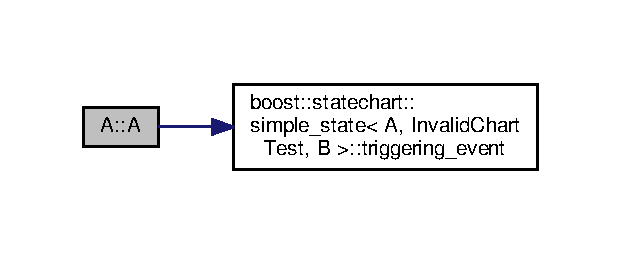
\includegraphics[width=298pt]{struct_a_aa7bea9bf6fe35fcde90da1f5a06ba4e9_cgraph}
\end{center}
\end{figure}
\mbox{\Hypertarget{struct_a_a8d74412b1ff05d7493b4c546795bf405}\label{struct_a_a8d74412b1ff05d7493b4c546795bf405}} 
\index{A@{A}!````~A@{$\sim$A}}
\index{````~A@{$\sim$A}!A@{A}}
\subsubsection{\texorpdfstring{$\sim$\+A()}{~A()}}
{\footnotesize\ttfamily A\+::$\sim$A (\begin{DoxyParamCaption}{ }\end{DoxyParamCaption})\hspace{0.3cm}{\ttfamily [inline]}}

Here is the call graph for this function\+:
\nopagebreak
\begin{figure}[H]
\begin{center}
\leavevmode
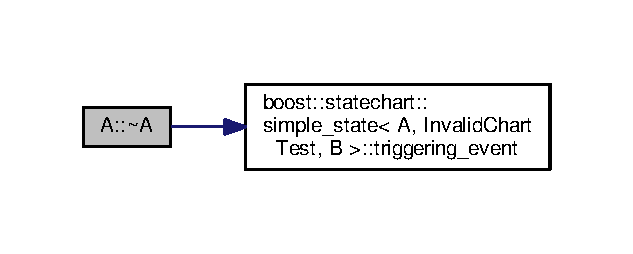
\includegraphics[width=304pt]{struct_a_a8d74412b1ff05d7493b4c546795bf405_cgraph}
\end{center}
\end{figure}


\subsection{Member Function Documentation}
\mbox{\Hypertarget{struct_a_a7811ed8883449fde0d5f59bd2ebf3de5}\label{struct_a_a7811ed8883449fde0d5f59bd2ebf3de5}} 
\index{A@{A}!Increment\+Count@{Increment\+Count}}
\index{Increment\+Count@{Increment\+Count}!A@{A}}
\subsubsection{\texorpdfstring{Increment\+Count()}{IncrementCount()}\hspace{0.1cm}{\footnotesize\ttfamily [1/3]}}
{\footnotesize\ttfamily void A\+::\+Increment\+Count (\begin{DoxyParamCaption}\item[{const \mbox{\hyperlink{classboost_1_1statechart_1_1event__base}{sc\+::event\+\_\+base}} \&}]{ }\end{DoxyParamCaption})\hspace{0.3cm}{\ttfamily [inline]}}

\mbox{\Hypertarget{struct_a_afb9a418cf38492b6c1c50dbe1df1e741}\label{struct_a_afb9a418cf38492b6c1c50dbe1df1e741}} 
\index{A@{A}!Increment\+Count@{Increment\+Count}}
\index{Increment\+Count@{Increment\+Count}!A@{A}}
\subsubsection{\texorpdfstring{Increment\+Count()}{IncrementCount()}\hspace{0.1cm}{\footnotesize\ttfamily [2/3]}}
{\footnotesize\ttfamily void A\+::\+Increment\+Count (\begin{DoxyParamCaption}\item[{const \mbox{\hyperlink{struct_e}{E}} \&}]{ }\end{DoxyParamCaption})\hspace{0.3cm}{\ttfamily [inline]}}

\mbox{\Hypertarget{struct_a_abf23b59d725012e048a7f5e3ae1c52ca}\label{struct_a_abf23b59d725012e048a7f5e3ae1c52ca}} 
\index{A@{A}!Increment\+Count@{Increment\+Count}}
\index{Increment\+Count@{Increment\+Count}!A@{A}}
\subsubsection{\texorpdfstring{Increment\+Count()}{IncrementCount()}\hspace{0.1cm}{\footnotesize\ttfamily [3/3]}}
{\footnotesize\ttfamily void A\+::\+Increment\+Count (\begin{DoxyParamCaption}\item[{const \mbox{\hyperlink{struct_g}{G}} \&}]{ }\end{DoxyParamCaption})\hspace{0.3cm}{\ttfamily [inline]}}

\mbox{\Hypertarget{struct_a_adf85098984576064f58c36259a6b58c9}\label{struct_a_adf85098984576064f58c36259a6b58c9}} 
\index{A@{A}!react@{react}}
\index{react@{react}!A@{A}}
\subsubsection{\texorpdfstring{react()}{react()}\hspace{0.1cm}{\footnotesize\ttfamily [1/11]}}
{\footnotesize\ttfamily \mbox{\hyperlink{namespaceboost_1_1statechart_abe807f6598b614d6d87bb951ecd92331}{sc\+::result}} A\+::react (\begin{DoxyParamCaption}\item[{const \mbox{\hyperlink{struct_ev_x}{EvX}} \&}]{ }\end{DoxyParamCaption})\hspace{0.3cm}{\ttfamily [inline]}}

Here is the call graph for this function\+:
\nopagebreak
\begin{figure}[H]
\begin{center}
\leavevmode
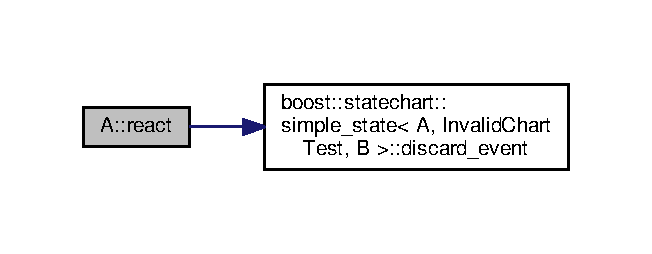
\includegraphics[width=313pt]{struct_a_adf85098984576064f58c36259a6b58c9_cgraph}
\end{center}
\end{figure}
\mbox{\Hypertarget{struct_a_adf85098984576064f58c36259a6b58c9}\label{struct_a_adf85098984576064f58c36259a6b58c9}} 
\index{A@{A}!react@{react}}
\index{react@{react}!A@{A}}
\subsubsection{\texorpdfstring{react()}{react()}\hspace{0.1cm}{\footnotesize\ttfamily [2/11]}}
{\footnotesize\ttfamily \mbox{\hyperlink{namespaceboost_1_1statechart_abe807f6598b614d6d87bb951ecd92331}{sc\+::result}} A\+::react (\begin{DoxyParamCaption}\item[{const \mbox{\hyperlink{struct_ev_x}{EvX}} \&}]{ }\end{DoxyParamCaption})\hspace{0.3cm}{\ttfamily [inline]}}

Here is the call graph for this function\+:
\nopagebreak
\begin{figure}[H]
\begin{center}
\leavevmode
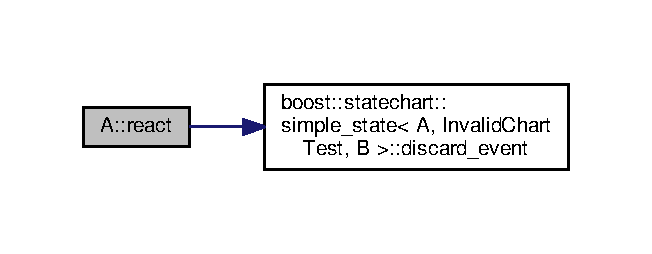
\includegraphics[width=313pt]{struct_a_adf85098984576064f58c36259a6b58c9_cgraph}
\end{center}
\end{figure}
\mbox{\Hypertarget{struct_a_a7eaee5c73ef0a2a5fb0886b4b1bc4a48}\label{struct_a_a7eaee5c73ef0a2a5fb0886b4b1bc4a48}} 
\index{A@{A}!react@{react}}
\index{react@{react}!A@{A}}
\subsubsection{\texorpdfstring{react()}{react()}\hspace{0.1cm}{\footnotesize\ttfamily [3/11]}}
{\footnotesize\ttfamily \mbox{\hyperlink{namespaceboost_1_1statechart_abe807f6598b614d6d87bb951ecd92331}{sc\+::result}} A\+::react (\begin{DoxyParamCaption}\item[{const \mbox{\hyperlink{struct_e}{E}} \&}]{ }\end{DoxyParamCaption})\hspace{0.3cm}{\ttfamily [inline]}}

Here is the call graph for this function\+:
\nopagebreak
\begin{figure}[H]
\begin{center}
\leavevmode
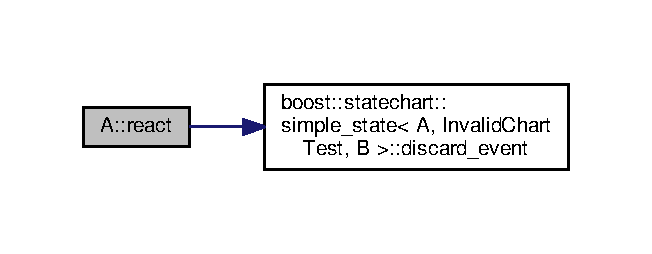
\includegraphics[width=313pt]{struct_a_a7eaee5c73ef0a2a5fb0886b4b1bc4a48_cgraph}
\end{center}
\end{figure}
\mbox{\Hypertarget{struct_a_a7eaee5c73ef0a2a5fb0886b4b1bc4a48}\label{struct_a_a7eaee5c73ef0a2a5fb0886b4b1bc4a48}} 
\index{A@{A}!react@{react}}
\index{react@{react}!A@{A}}
\subsubsection{\texorpdfstring{react()}{react()}\hspace{0.1cm}{\footnotesize\ttfamily [4/11]}}
{\footnotesize\ttfamily \mbox{\hyperlink{namespaceboost_1_1statechart_abe807f6598b614d6d87bb951ecd92331}{sc\+::result}} A\+::react (\begin{DoxyParamCaption}\item[{const \mbox{\hyperlink{struct_e}{E}} \&}]{ }\end{DoxyParamCaption})\hspace{0.3cm}{\ttfamily [inline]}}

Here is the call graph for this function\+:
\nopagebreak
\begin{figure}[H]
\begin{center}
\leavevmode
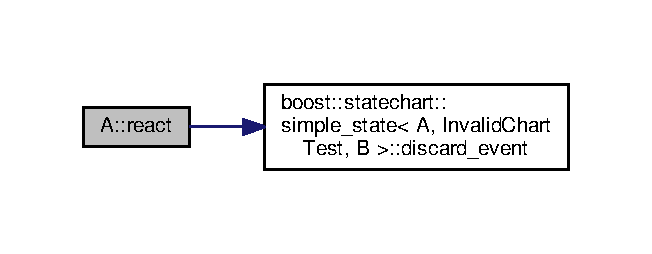
\includegraphics[width=313pt]{struct_a_a7eaee5c73ef0a2a5fb0886b4b1bc4a48_cgraph}
\end{center}
\end{figure}
\mbox{\Hypertarget{struct_a_a38e1d44955d46136ca8ea912ae202a52}\label{struct_a_a38e1d44955d46136ca8ea912ae202a52}} 
\index{A@{A}!react@{react}}
\index{react@{react}!A@{A}}
\subsubsection{\texorpdfstring{react()}{react()}\hspace{0.1cm}{\footnotesize\ttfamily [5/11]}}
{\footnotesize\ttfamily \mbox{\hyperlink{namespaceboost_1_1statechart_abe807f6598b614d6d87bb951ecd92331}{sc\+::result}} A\+::react (\begin{DoxyParamCaption}\item[{const \mbox{\hyperlink{struct_ev_discard_never}{Ev\+Discard\+Never}} \&}]{ }\end{DoxyParamCaption})\hspace{0.3cm}{\ttfamily [inline]}}

Here is the call graph for this function\+:
\nopagebreak
\begin{figure}[H]
\begin{center}
\leavevmode
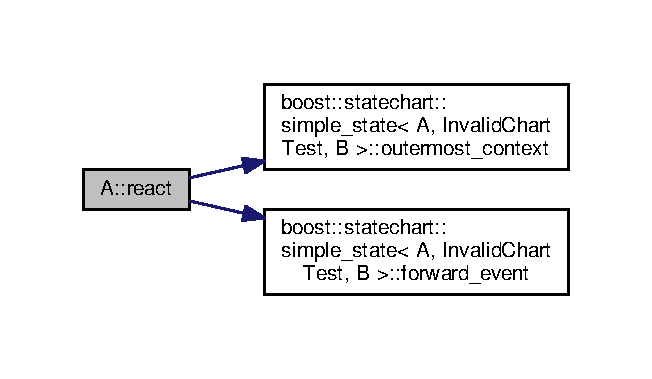
\includegraphics[width=313pt]{struct_a_a38e1d44955d46136ca8ea912ae202a52_cgraph}
\end{center}
\end{figure}
\mbox{\Hypertarget{struct_a_a59fa7dccf0b31b8a69a6e5607be864d1}\label{struct_a_a59fa7dccf0b31b8a69a6e5607be864d1}} 
\index{A@{A}!react@{react}}
\index{react@{react}!A@{A}}
\subsubsection{\texorpdfstring{react()}{react()}\hspace{0.1cm}{\footnotesize\ttfamily [6/11]}}
{\footnotesize\ttfamily \mbox{\hyperlink{namespaceboost_1_1statechart_abe807f6598b614d6d87bb951ecd92331}{sc\+::result}} A\+::react (\begin{DoxyParamCaption}\item[{const \mbox{\hyperlink{struct_ev_discard_in_b}{Ev\+Discard\+InB}} \&}]{ }\end{DoxyParamCaption})\hspace{0.3cm}{\ttfamily [inline]}}

Here is the call graph for this function\+:
\nopagebreak
\begin{figure}[H]
\begin{center}
\leavevmode
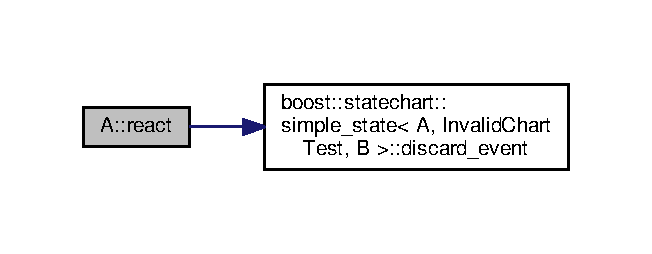
\includegraphics[width=313pt]{struct_a_a59fa7dccf0b31b8a69a6e5607be864d1_cgraph}
\end{center}
\end{figure}
\mbox{\Hypertarget{struct_a_aeebabda5b0df22ae3c95fb0415135aa6}\label{struct_a_aeebabda5b0df22ae3c95fb0415135aa6}} 
\index{A@{A}!react@{react}}
\index{react@{react}!A@{A}}
\subsubsection{\texorpdfstring{react()}{react()}\hspace{0.1cm}{\footnotesize\ttfamily [7/11]}}
{\footnotesize\ttfamily \mbox{\hyperlink{namespaceboost_1_1statechart_abe807f6598b614d6d87bb951ecd92331}{sc\+::result}} A\+::react (\begin{DoxyParamCaption}\item[{const \mbox{\hyperlink{struct_ev_discard_in_d}{Ev\+Discard\+InD}} \&}]{ }\end{DoxyParamCaption})\hspace{0.3cm}{\ttfamily [inline]}}

Here is the call graph for this function\+:
\nopagebreak
\begin{figure}[H]
\begin{center}
\leavevmode
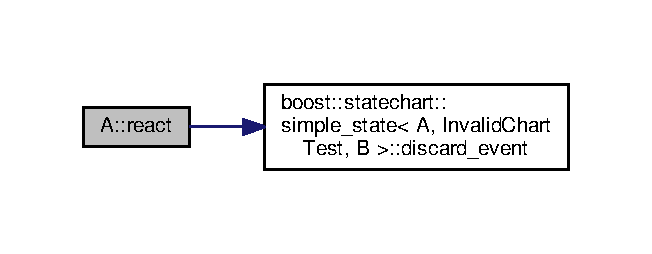
\includegraphics[width=313pt]{struct_a_aeebabda5b0df22ae3c95fb0415135aa6_cgraph}
\end{center}
\end{figure}
\mbox{\Hypertarget{struct_a_a088ea5e2fe4c12cb13a3151cf040face}\label{struct_a_a088ea5e2fe4c12cb13a3151cf040face}} 
\index{A@{A}!react@{react}}
\index{react@{react}!A@{A}}
\subsubsection{\texorpdfstring{react()}{react()}\hspace{0.1cm}{\footnotesize\ttfamily [8/11]}}
{\footnotesize\ttfamily \mbox{\hyperlink{namespaceboost_1_1statechart_abe807f6598b614d6d87bb951ecd92331}{sc\+::result}} A\+::react (\begin{DoxyParamCaption}\item[{const \mbox{\hyperlink{struct_ev_defer}{Ev\+Defer}} \&}]{ }\end{DoxyParamCaption})\hspace{0.3cm}{\ttfamily [inline]}}

Here is the call graph for this function\+:
\nopagebreak
\begin{figure}[H]
\begin{center}
\leavevmode
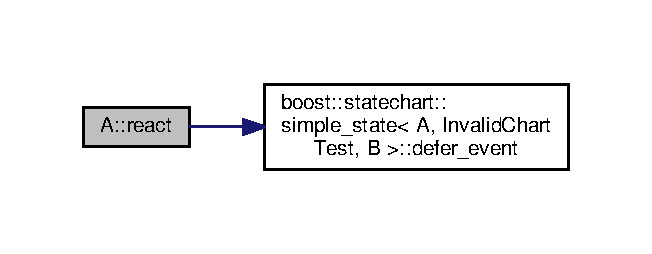
\includegraphics[width=313pt]{struct_a_a088ea5e2fe4c12cb13a3151cf040face_cgraph}
\end{center}
\end{figure}
\mbox{\Hypertarget{struct_a_a43a91cc21bb007d57f7cacb94c9da395}\label{struct_a_a43a91cc21bb007d57f7cacb94c9da395}} 
\index{A@{A}!react@{react}}
\index{react@{react}!A@{A}}
\subsubsection{\texorpdfstring{react()}{react()}\hspace{0.1cm}{\footnotesize\ttfamily [9/11]}}
{\footnotesize\ttfamily \mbox{\hyperlink{namespaceboost_1_1statechart_abe807f6598b614d6d87bb951ecd92331}{sc\+::result}} A\+::react (\begin{DoxyParamCaption}\item[{const \mbox{\hyperlink{struct_ev_terminate}{Ev\+Terminate}} \&}]{ }\end{DoxyParamCaption})\hspace{0.3cm}{\ttfamily [inline]}}

Here is the call graph for this function\+:
\nopagebreak
\begin{figure}[H]
\begin{center}
\leavevmode
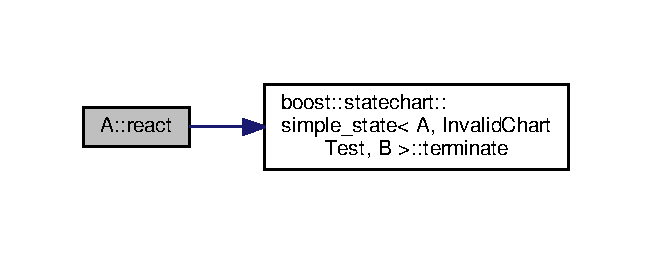
\includegraphics[width=313pt]{struct_a_a43a91cc21bb007d57f7cacb94c9da395_cgraph}
\end{center}
\end{figure}
\mbox{\Hypertarget{struct_a_a93cff2d52bb90cd3d97117abfc5ed3a6}\label{struct_a_a93cff2d52bb90cd3d97117abfc5ed3a6}} 
\index{A@{A}!react@{react}}
\index{react@{react}!A@{A}}
\subsubsection{\texorpdfstring{react()}{react()}\hspace{0.1cm}{\footnotesize\ttfamily [10/11]}}
{\footnotesize\ttfamily \mbox{\hyperlink{namespaceboost_1_1statechart_abe807f6598b614d6d87bb951ecd92331}{sc\+::result}} A\+::react (\begin{DoxyParamCaption}\item[{const \mbox{\hyperlink{struct_ev_transit}{Ev\+Transit}} \&}]{ }\end{DoxyParamCaption})\hspace{0.3cm}{\ttfamily [inline]}}

\mbox{\Hypertarget{struct_a_a22e1cf6871b994db83aec743fbf6f5d0}\label{struct_a_a22e1cf6871b994db83aec743fbf6f5d0}} 
\index{A@{A}!react@{react}}
\index{react@{react}!A@{A}}
\subsubsection{\texorpdfstring{react()}{react()}\hspace{0.1cm}{\footnotesize\ttfamily [11/11]}}
{\footnotesize\ttfamily \mbox{\hyperlink{namespaceboost_1_1statechart_abe807f6598b614d6d87bb951ecd92331}{sc\+::result}} A\+::react (\begin{DoxyParamCaption}\item[{const \mbox{\hyperlink{struct_ev_transit_with_action}{Ev\+Transit\+With\+Action}} \&}]{evt }\end{DoxyParamCaption})\hspace{0.3cm}{\ttfamily [inline]}}

Here is the call graph for this function\+:
\nopagebreak
\begin{figure}[H]
\begin{center}
\leavevmode
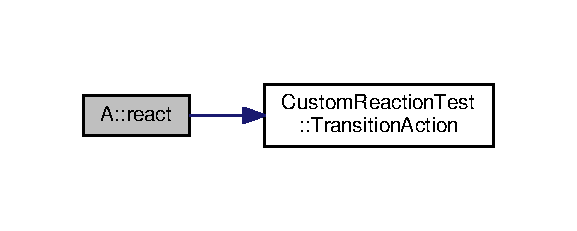
\includegraphics[width=277pt]{struct_a_a22e1cf6871b994db83aec743fbf6f5d0_cgraph}
\end{center}
\end{figure}


\subsection{Member Data Documentation}
\mbox{\Hypertarget{struct_a_a3c06744fc190a128fd536cf61f15e88b}\label{struct_a_a3c06744fc190a128fd536cf61f15e88b}} 
\index{A@{A}!event\+Count\+\_\+@{event\+Count\+\_\+}}
\index{event\+Count\+\_\+@{event\+Count\+\_\+}!A@{A}}
\subsubsection{\texorpdfstring{event\+Count\+\_\+}{eventCount\_}}
{\footnotesize\ttfamily unsigned int A\+::event\+Count\+\_\+}



The documentation for this struct was generated from the following files\+:\begin{DoxyCompactItemize}
\item 
test/\mbox{\hyperlink{_custom_reaction_test_8cpp}{Custom\+Reaction\+Test.\+cpp}}\item 
test/\mbox{\hyperlink{_history_test_8cpp}{History\+Test.\+cpp}}\item 
test/\mbox{\hyperlink{_inconsistent_history_test2_8cpp}{Inconsistent\+History\+Test2.\+cpp}}\item 
test/\mbox{\hyperlink{_inconsistent_history_test4_8cpp}{Inconsistent\+History\+Test4.\+cpp}}\item 
test/\mbox{\hyperlink{_inconsistent_history_test6_8cpp}{Inconsistent\+History\+Test6.\+cpp}}\item 
test/\mbox{\hyperlink{_inconsistent_history_test8_8cpp}{Inconsistent\+History\+Test8.\+cpp}}\item 
test/\mbox{\hyperlink{_in_state_reaction_test_8cpp}{In\+State\+Reaction\+Test.\+cpp}}\item 
test/\mbox{\hyperlink{_invalid_result_assign_test_8cpp}{Invalid\+Result\+Assign\+Test.\+cpp}}\item 
test/\mbox{\hyperlink{_invalid_result_copy_test_8cpp}{Invalid\+Result\+Copy\+Test.\+cpp}}\item 
test/\mbox{\hyperlink{_state_cast_test_8cpp}{State\+Cast\+Test.\+cpp}}\item 
test/\mbox{\hyperlink{_state_iteration_test_8cpp}{State\+Iteration\+Test.\+cpp}}\item 
test/\mbox{\hyperlink{_termination_test_8cpp}{Termination\+Test.\+cpp}}\item 
test/\mbox{\hyperlink{_triggering_event_test_8cpp}{Triggering\+Event\+Test.\+cpp}}\end{DoxyCompactItemize}

\hypertarget{struct_active}{}\section{Active Struct Reference}
\label{struct_active}\index{Active@{Active}}


Inheritance diagram for Active\+:
\nopagebreak
\begin{figure}[H]
\begin{center}
\leavevmode
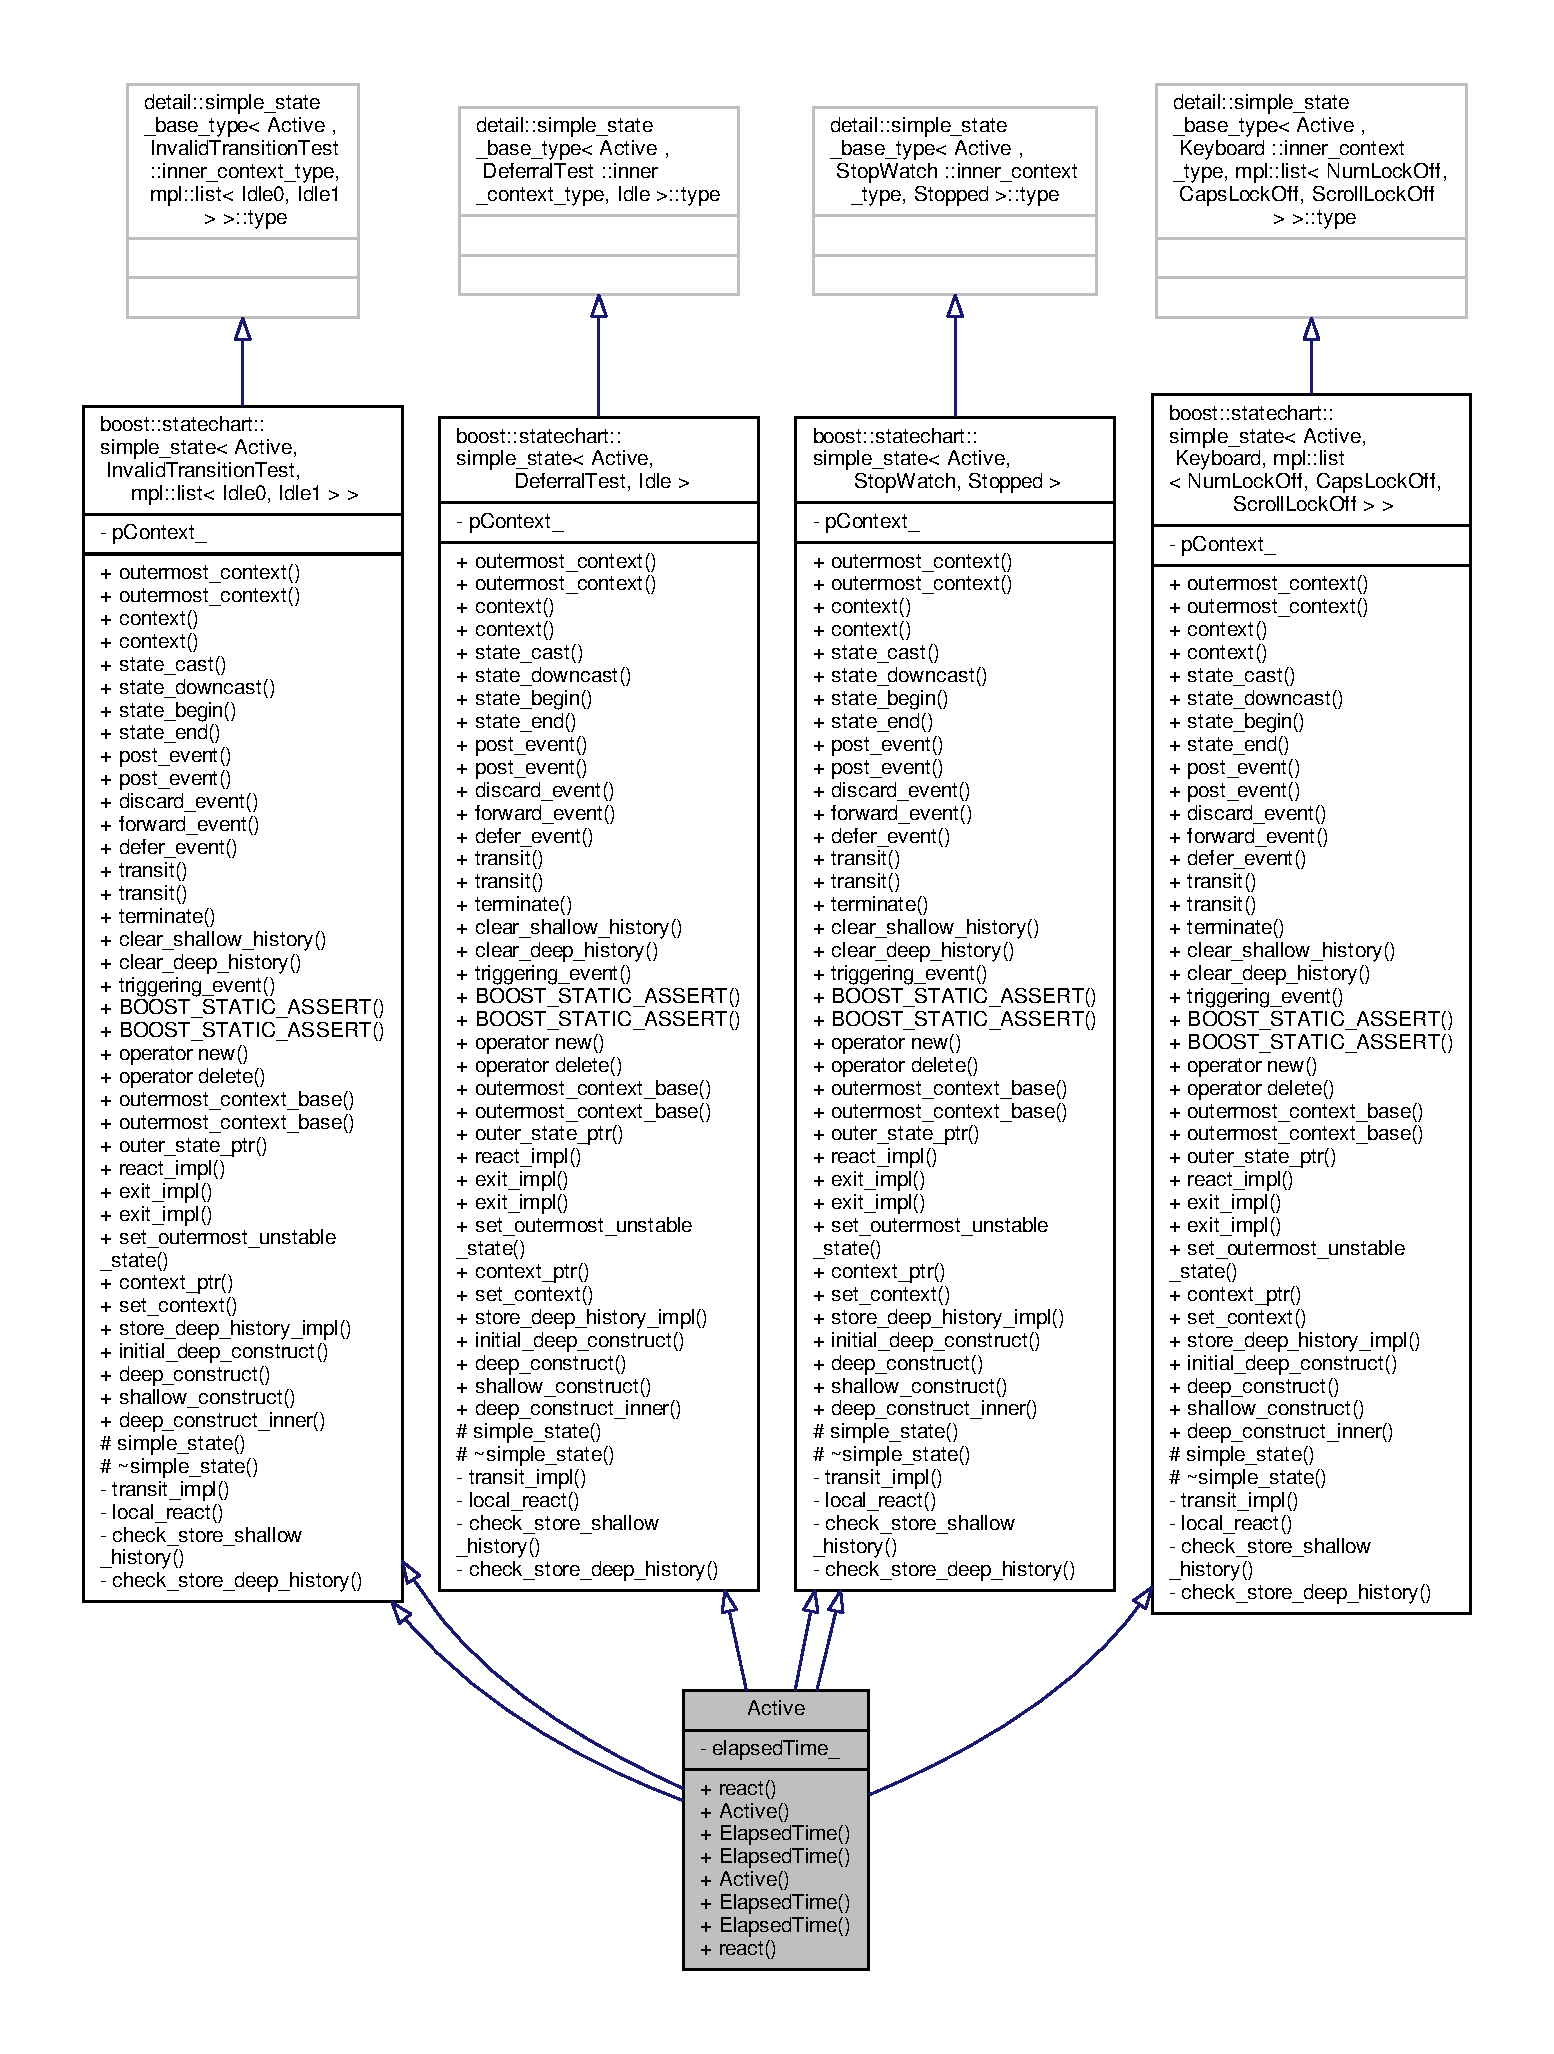
\includegraphics[width=350pt]{struct_active__inherit__graph}
\end{center}
\end{figure}


Collaboration diagram for Active\+:
\nopagebreak
\begin{figure}[H]
\begin{center}
\leavevmode
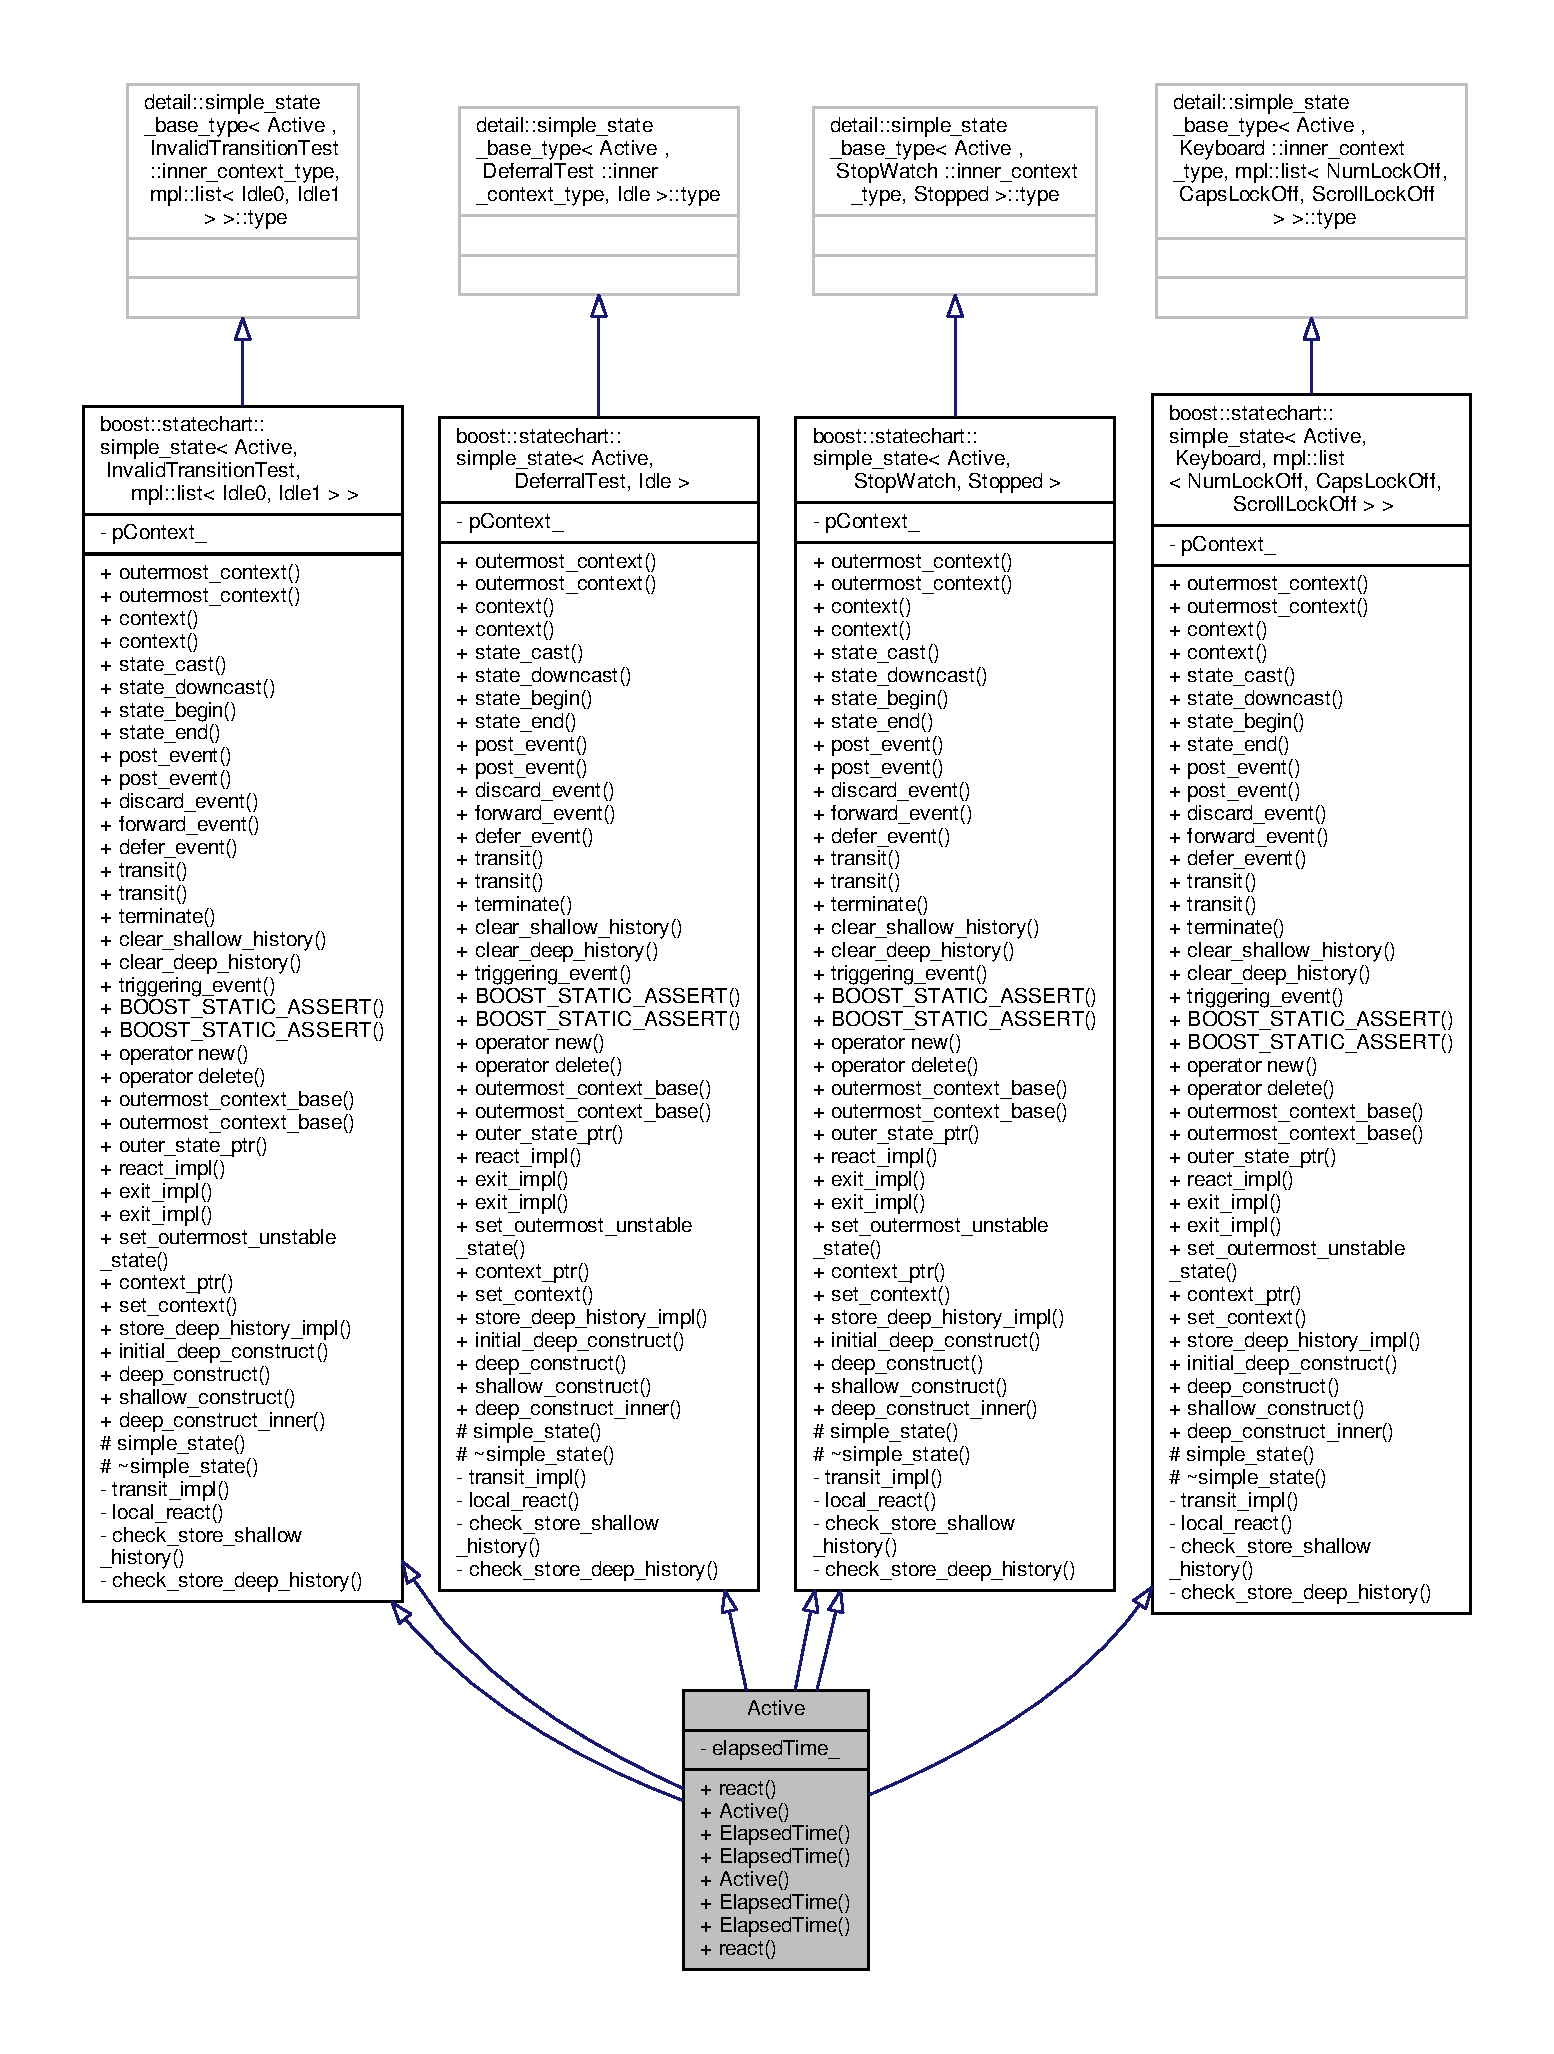
\includegraphics[width=350pt]{struct_active__coll__graph}
\end{center}
\end{figure}
\subsection*{Public Types}
\begin{DoxyCompactItemize}
\item 
typedef \mbox{\hyperlink{classboost_1_1statechart_1_1custom__reaction}{sc\+::custom\+\_\+reaction}}$<$ \mbox{\hyperlink{struct_ev_request_shutdown}{Ev\+Request\+Shutdown}} $>$ \mbox{\hyperlink{struct_active_a628dd827d0faf3cd002f59a8d17f189d}{reactions}}
\item 
typedef \mbox{\hyperlink{classboost_1_1statechart_1_1transition}{sc\+::transition}}$<$ \mbox{\hyperlink{struct_ev_reset}{Ev\+Reset}}, \mbox{\hyperlink{struct_active}{Active}} $>$ \mbox{\hyperlink{struct_active_a86282569cdd6a34df7d2580364c79857}{reactions}}
\item 
typedef \mbox{\hyperlink{classboost_1_1statechart_1_1transition}{sc\+::transition}}$<$ \mbox{\hyperlink{struct_ev_reset}{Ev\+Reset}}, \mbox{\hyperlink{struct_active}{Active}} $>$ \mbox{\hyperlink{struct_active_a86282569cdd6a34df7d2580364c79857}{reactions}}
\item 
typedef mpl\+::list$<$ \mbox{\hyperlink{classboost_1_1statechart_1_1custom__reaction}{sc\+::custom\+\_\+reaction}}$<$ \mbox{\hyperlink{struct_ev_leaf_deferred}{Ev\+Leaf\+Deferred}} $>$, \mbox{\hyperlink{classboost_1_1statechart_1_1deferral}{sc\+::deferral}}$<$ \mbox{\hyperlink{struct_ev_node_deferred}{Ev\+Node\+Deferred}} $>$, \mbox{\hyperlink{classboost_1_1statechart_1_1transition}{sc\+::transition}}$<$ \mbox{\hyperlink{struct_ev_destroy}{Ev\+Destroy}}, \mbox{\hyperlink{struct_dead}{Dead}} $>$ $>$ \mbox{\hyperlink{struct_active_a3f41c16a9522a432b7c51738621d8650}{reactions}}
\end{DoxyCompactItemize}
\subsection*{Public Member Functions}
\begin{DoxyCompactItemize}
\item 
\mbox{\hyperlink{namespaceboost_1_1statechart_abe807f6598b614d6d87bb951ecd92331}{sc\+::result}} \mbox{\hyperlink{struct_active_afe9a0390ef2231d6e36bc7ca49e5220a}{react}} (const \mbox{\hyperlink{struct_ev_request_shutdown}{Ev\+Request\+Shutdown}} \&)
\item 
\mbox{\hyperlink{struct_active_aa276bfdc4f8f0ec3fd8a8a3a2cedab1e}{Active}} ()
\item 
double \& \mbox{\hyperlink{struct_active_a61b84526303d31ed5d4d0b64efa15996}{Elapsed\+Time}} ()
\item 
double \mbox{\hyperlink{struct_active_adc392561063b506262e24bca87a74f43}{Elapsed\+Time}} () const
\item 
\mbox{\hyperlink{struct_active_aa276bfdc4f8f0ec3fd8a8a3a2cedab1e}{Active}} ()
\item 
double \& \mbox{\hyperlink{struct_active_a61b84526303d31ed5d4d0b64efa15996}{Elapsed\+Time}} ()
\item 
double \mbox{\hyperlink{struct_active_adc392561063b506262e24bca87a74f43}{Elapsed\+Time}} () const
\item 
\mbox{\hyperlink{namespaceboost_1_1statechart_abe807f6598b614d6d87bb951ecd92331}{sc\+::result}} \mbox{\hyperlink{struct_active_a173c792f4e486c497ad10ebc5add135e}{react}} (const \mbox{\hyperlink{struct_ev_leaf_deferred}{Ev\+Leaf\+Deferred}} \&)
\end{DoxyCompactItemize}
\subsection*{Private Attributes}
\begin{DoxyCompactItemize}
\item 
double \mbox{\hyperlink{struct_active_a3f50dfab6f5983a20aedd5a3cb6a49c9}{elapsed\+Time\+\_\+}}
\end{DoxyCompactItemize}
\subsection*{Additional Inherited Members}


\subsection{Member Typedef Documentation}
\mbox{\Hypertarget{struct_active_a628dd827d0faf3cd002f59a8d17f189d}\label{struct_active_a628dd827d0faf3cd002f59a8d17f189d}} 
\index{Active@{Active}!reactions@{reactions}}
\index{reactions@{reactions}!Active@{Active}}
\subsubsection{\texorpdfstring{reactions}{reactions}\hspace{0.1cm}{\footnotesize\ttfamily [1/4]}}
{\footnotesize\ttfamily typedef \mbox{\hyperlink{classboost_1_1statechart_1_1custom__reaction}{sc\+::custom\+\_\+reaction}}$<$ \mbox{\hyperlink{struct_ev_request_shutdown}{Ev\+Request\+Shutdown}} $>$ \mbox{\hyperlink{struct_active_a628dd827d0faf3cd002f59a8d17f189d}{Active\+::reactions}}}

\mbox{\Hypertarget{struct_active_a3f41c16a9522a432b7c51738621d8650}\label{struct_active_a3f41c16a9522a432b7c51738621d8650}} 
\index{Active@{Active}!reactions@{reactions}}
\index{reactions@{reactions}!Active@{Active}}
\subsubsection{\texorpdfstring{reactions}{reactions}\hspace{0.1cm}{\footnotesize\ttfamily [2/4]}}
{\footnotesize\ttfamily typedef mpl\+::list$<$ \mbox{\hyperlink{classboost_1_1statechart_1_1custom__reaction}{sc\+::custom\+\_\+reaction}}$<$ \mbox{\hyperlink{struct_ev_leaf_deferred}{Ev\+Leaf\+Deferred}} $>$, \mbox{\hyperlink{classboost_1_1statechart_1_1deferral}{sc\+::deferral}}$<$ \mbox{\hyperlink{struct_ev_node_deferred}{Ev\+Node\+Deferred}} $>$, \mbox{\hyperlink{classboost_1_1statechart_1_1transition}{sc\+::transition}}$<$ \mbox{\hyperlink{struct_ev_destroy}{Ev\+Destroy}}, \mbox{\hyperlink{struct_dead}{Dead}} $>$ $>$ \mbox{\hyperlink{struct_active_a628dd827d0faf3cd002f59a8d17f189d}{Active\+::reactions}}}

\mbox{\Hypertarget{struct_active_a86282569cdd6a34df7d2580364c79857}\label{struct_active_a86282569cdd6a34df7d2580364c79857}} 
\index{Active@{Active}!reactions@{reactions}}
\index{reactions@{reactions}!Active@{Active}}
\subsubsection{\texorpdfstring{reactions}{reactions}\hspace{0.1cm}{\footnotesize\ttfamily [3/4]}}
{\footnotesize\ttfamily typedef \mbox{\hyperlink{classboost_1_1statechart_1_1transition}{sc\+::transition}}$<$ \mbox{\hyperlink{struct_ev_reset}{Ev\+Reset}}, \mbox{\hyperlink{struct_active}{Active}} $>$ \mbox{\hyperlink{struct_active_a628dd827d0faf3cd002f59a8d17f189d}{Active\+::reactions}}}

\mbox{\Hypertarget{struct_active_a86282569cdd6a34df7d2580364c79857}\label{struct_active_a86282569cdd6a34df7d2580364c79857}} 
\index{Active@{Active}!reactions@{reactions}}
\index{reactions@{reactions}!Active@{Active}}
\subsubsection{\texorpdfstring{reactions}{reactions}\hspace{0.1cm}{\footnotesize\ttfamily [4/4]}}
{\footnotesize\ttfamily typedef \mbox{\hyperlink{classboost_1_1statechart_1_1transition}{sc\+::transition}}$<$ \mbox{\hyperlink{struct_ev_reset}{Ev\+Reset}}, \mbox{\hyperlink{struct_active}{Active}} $>$ \mbox{\hyperlink{struct_active_a628dd827d0faf3cd002f59a8d17f189d}{Active\+::reactions}}}



\subsection{Constructor \& Destructor Documentation}
\mbox{\Hypertarget{struct_active_aa276bfdc4f8f0ec3fd8a8a3a2cedab1e}\label{struct_active_aa276bfdc4f8f0ec3fd8a8a3a2cedab1e}} 
\index{Active@{Active}!Active@{Active}}
\index{Active@{Active}!Active@{Active}}
\subsubsection{\texorpdfstring{Active()}{Active()}\hspace{0.1cm}{\footnotesize\ttfamily [1/2]}}
{\footnotesize\ttfamily Active\+::\+Active (\begin{DoxyParamCaption}{ }\end{DoxyParamCaption})\hspace{0.3cm}{\ttfamily [inline]}}

\mbox{\Hypertarget{struct_active_aa276bfdc4f8f0ec3fd8a8a3a2cedab1e}\label{struct_active_aa276bfdc4f8f0ec3fd8a8a3a2cedab1e}} 
\index{Active@{Active}!Active@{Active}}
\index{Active@{Active}!Active@{Active}}
\subsubsection{\texorpdfstring{Active()}{Active()}\hspace{0.1cm}{\footnotesize\ttfamily [2/2]}}
{\footnotesize\ttfamily Active\+::\+Active (\begin{DoxyParamCaption}{ }\end{DoxyParamCaption})\hspace{0.3cm}{\ttfamily [inline]}}



\subsection{Member Function Documentation}
\mbox{\Hypertarget{struct_active_a61b84526303d31ed5d4d0b64efa15996}\label{struct_active_a61b84526303d31ed5d4d0b64efa15996}} 
\index{Active@{Active}!Elapsed\+Time@{Elapsed\+Time}}
\index{Elapsed\+Time@{Elapsed\+Time}!Active@{Active}}
\subsubsection{\texorpdfstring{Elapsed\+Time()}{ElapsedTime()}\hspace{0.1cm}{\footnotesize\ttfamily [1/4]}}
{\footnotesize\ttfamily double\& Active\+::\+Elapsed\+Time (\begin{DoxyParamCaption}{ }\end{DoxyParamCaption})\hspace{0.3cm}{\ttfamily [inline]}}

\mbox{\Hypertarget{struct_active_adc392561063b506262e24bca87a74f43}\label{struct_active_adc392561063b506262e24bca87a74f43}} 
\index{Active@{Active}!Elapsed\+Time@{Elapsed\+Time}}
\index{Elapsed\+Time@{Elapsed\+Time}!Active@{Active}}
\subsubsection{\texorpdfstring{Elapsed\+Time()}{ElapsedTime()}\hspace{0.1cm}{\footnotesize\ttfamily [2/4]}}
{\footnotesize\ttfamily double Active\+::\+Elapsed\+Time (\begin{DoxyParamCaption}{ }\end{DoxyParamCaption}) const\hspace{0.3cm}{\ttfamily [inline]}}

\mbox{\Hypertarget{struct_active_a61b84526303d31ed5d4d0b64efa15996}\label{struct_active_a61b84526303d31ed5d4d0b64efa15996}} 
\index{Active@{Active}!Elapsed\+Time@{Elapsed\+Time}}
\index{Elapsed\+Time@{Elapsed\+Time}!Active@{Active}}
\subsubsection{\texorpdfstring{Elapsed\+Time()}{ElapsedTime()}\hspace{0.1cm}{\footnotesize\ttfamily [3/4]}}
{\footnotesize\ttfamily double\& Active\+::\+Elapsed\+Time (\begin{DoxyParamCaption}{ }\end{DoxyParamCaption})\hspace{0.3cm}{\ttfamily [inline]}}

\mbox{\Hypertarget{struct_active_adc392561063b506262e24bca87a74f43}\label{struct_active_adc392561063b506262e24bca87a74f43}} 
\index{Active@{Active}!Elapsed\+Time@{Elapsed\+Time}}
\index{Elapsed\+Time@{Elapsed\+Time}!Active@{Active}}
\subsubsection{\texorpdfstring{Elapsed\+Time()}{ElapsedTime()}\hspace{0.1cm}{\footnotesize\ttfamily [4/4]}}
{\footnotesize\ttfamily double Active\+::\+Elapsed\+Time (\begin{DoxyParamCaption}{ }\end{DoxyParamCaption}) const\hspace{0.3cm}{\ttfamily [inline]}}

\mbox{\Hypertarget{struct_active_afe9a0390ef2231d6e36bc7ca49e5220a}\label{struct_active_afe9a0390ef2231d6e36bc7ca49e5220a}} 
\index{Active@{Active}!react@{react}}
\index{react@{react}!Active@{Active}}
\subsubsection{\texorpdfstring{react()}{react()}\hspace{0.1cm}{\footnotesize\ttfamily [1/2]}}
{\footnotesize\ttfamily \mbox{\hyperlink{namespaceboost_1_1statechart_abe807f6598b614d6d87bb951ecd92331}{sc\+::result}} Active\+::react (\begin{DoxyParamCaption}\item[{const \mbox{\hyperlink{struct_ev_request_shutdown}{Ev\+Request\+Shutdown}} \&}]{ }\end{DoxyParamCaption})}

Here is the call graph for this function\+:
\nopagebreak
\begin{figure}[H]
\begin{center}
\leavevmode
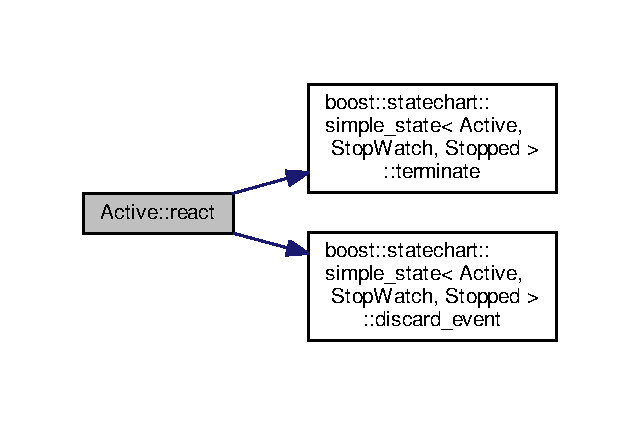
\includegraphics[width=307pt]{struct_active_afe9a0390ef2231d6e36bc7ca49e5220a_cgraph}
\end{center}
\end{figure}
\mbox{\Hypertarget{struct_active_a173c792f4e486c497ad10ebc5add135e}\label{struct_active_a173c792f4e486c497ad10ebc5add135e}} 
\index{Active@{Active}!react@{react}}
\index{react@{react}!Active@{Active}}
\subsubsection{\texorpdfstring{react()}{react()}\hspace{0.1cm}{\footnotesize\ttfamily [2/2]}}
{\footnotesize\ttfamily \mbox{\hyperlink{namespaceboost_1_1statechart_abe807f6598b614d6d87bb951ecd92331}{sc\+::result}} Active\+::react (\begin{DoxyParamCaption}\item[{const \mbox{\hyperlink{struct_ev_leaf_deferred}{Ev\+Leaf\+Deferred}} \&}]{ }\end{DoxyParamCaption})\hspace{0.3cm}{\ttfamily [inline]}}

Here is the call graph for this function\+:
\nopagebreak
\begin{figure}[H]
\begin{center}
\leavevmode
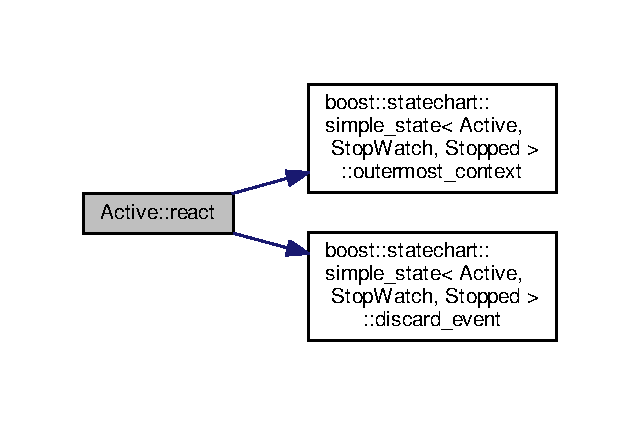
\includegraphics[width=307pt]{struct_active_a173c792f4e486c497ad10ebc5add135e_cgraph}
\end{center}
\end{figure}


\subsection{Member Data Documentation}
\mbox{\Hypertarget{struct_active_a3f50dfab6f5983a20aedd5a3cb6a49c9}\label{struct_active_a3f50dfab6f5983a20aedd5a3cb6a49c9}} 
\index{Active@{Active}!elapsed\+Time\+\_\+@{elapsed\+Time\+\_\+}}
\index{elapsed\+Time\+\_\+@{elapsed\+Time\+\_\+}!Active@{Active}}
\subsubsection{\texorpdfstring{elapsed\+Time\+\_\+}{elapsedTime\_}}
{\footnotesize\ttfamily double Active\+::elapsed\+Time\+\_\+\hspace{0.3cm}{\ttfamily [private]}}



The documentation for this struct was generated from the following files\+:\begin{DoxyCompactItemize}
\item 
example/\+Keyboard/\mbox{\hyperlink{_keyboard_8cpp}{Keyboard.\+cpp}}\item 
example/\+Stop\+Watch/\mbox{\hyperlink{_stop_watch_8cpp}{Stop\+Watch.\+cpp}}\item 
example/\+Stop\+Watch/\mbox{\hyperlink{_stop_watch2_8cpp}{Stop\+Watch2.\+cpp}}\item 
test/\mbox{\hyperlink{_deferral_test_8cpp}{Deferral\+Test.\+cpp}}\end{DoxyCompactItemize}

\hypertarget{structboost_1_1statechart_1_1detail_1_1unwrap__impl_1_1apply}{}\section{boost\+:\+:statechart\+:\+:detail\+:\+:unwrap\+\_\+impl$<$ Is\+Reference\+Wrapper $>$\+:\+:apply$<$ T $>$ Struct Template Reference}
\label{structboost_1_1statechart_1_1detail_1_1unwrap__impl_1_1apply}\index{boost\+::statechart\+::detail\+::unwrap\+\_\+impl$<$ Is\+Reference\+Wrapper $>$\+::apply$<$ T $>$@{boost\+::statechart\+::detail\+::unwrap\+\_\+impl$<$ Is\+Reference\+Wrapper $>$\+::apply$<$ T $>$}}


{\ttfamily \#include $<$processor\+\_\+container.\+hpp$>$}



Collaboration diagram for boost\+:\+:statechart\+:\+:detail\+:\+:unwrap\+\_\+impl$<$ Is\+Reference\+Wrapper $>$\+:\+:apply$<$ T $>$\+:
\nopagebreak
\begin{figure}[H]
\begin{center}
\leavevmode
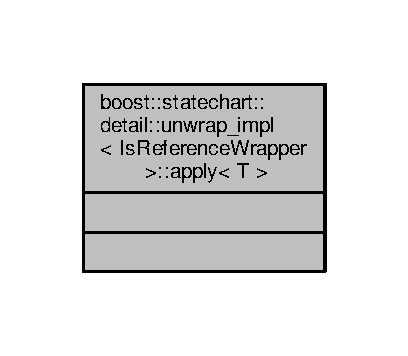
\includegraphics[width=196pt]{structboost_1_1statechart_1_1detail_1_1unwrap__impl_1_1apply__coll__graph}
\end{center}
\end{figure}
\subsection*{Public Types}
\begin{DoxyCompactItemize}
\item 
typedef T \mbox{\hyperlink{structboost_1_1statechart_1_1detail_1_1unwrap__impl_1_1apply_a876d02ff6c624d7c2cb5ed523eca7eef}{type}}
\end{DoxyCompactItemize}


\subsection{Member Typedef Documentation}
\mbox{\Hypertarget{structboost_1_1statechart_1_1detail_1_1unwrap__impl_1_1apply_a876d02ff6c624d7c2cb5ed523eca7eef}\label{structboost_1_1statechart_1_1detail_1_1unwrap__impl_1_1apply_a876d02ff6c624d7c2cb5ed523eca7eef}} 
\index{boost\+::statechart\+::detail\+::unwrap\+\_\+impl\+::apply@{boost\+::statechart\+::detail\+::unwrap\+\_\+impl\+::apply}!type@{type}}
\index{type@{type}!boost\+::statechart\+::detail\+::unwrap\+\_\+impl\+::apply@{boost\+::statechart\+::detail\+::unwrap\+\_\+impl\+::apply}}
\subsubsection{\texorpdfstring{type}{type}}
{\footnotesize\ttfamily template$<$bool Is\+Reference\+Wrapper$>$ \\
template$<$typename T $>$ \\
typedef T \mbox{\hyperlink{structboost_1_1statechart_1_1detail_1_1unwrap__impl}{boost\+::statechart\+::detail\+::unwrap\+\_\+impl}}$<$ Is\+Reference\+Wrapper $>$\+::\mbox{\hyperlink{structboost_1_1statechart_1_1detail_1_1unwrap__impl_1_1apply}{apply}}$<$ T $>$\+::\mbox{\hyperlink{structboost_1_1statechart_1_1detail_1_1unwrap__impl_1_1apply_a876d02ff6c624d7c2cb5ed523eca7eef}{type}}}



The documentation for this struct was generated from the following file\+:\begin{DoxyCompactItemize}
\item 
include/boost/statechart/\mbox{\hyperlink{processor__container_8hpp}{processor\+\_\+container.\+hpp}}\end{DoxyCompactItemize}

\hypertarget{structboost_1_1statechart_1_1detail_1_1unwrap__impl_3_01true_01_4_1_1apply}{}\section{boost\+:\+:statechart\+:\+:detail\+:\+:unwrap\+\_\+impl$<$ true $>$\+:\+:apply$<$ T $>$ Struct Template Reference}
\label{structboost_1_1statechart_1_1detail_1_1unwrap__impl_3_01true_01_4_1_1apply}\index{boost\+::statechart\+::detail\+::unwrap\+\_\+impl$<$ true $>$\+::apply$<$ T $>$@{boost\+::statechart\+::detail\+::unwrap\+\_\+impl$<$ true $>$\+::apply$<$ T $>$}}


{\ttfamily \#include $<$processor\+\_\+container.\+hpp$>$}



Collaboration diagram for boost\+:\+:statechart\+:\+:detail\+:\+:unwrap\+\_\+impl$<$ true $>$\+:\+:apply$<$ T $>$\+:
\nopagebreak
\begin{figure}[H]
\begin{center}
\leavevmode
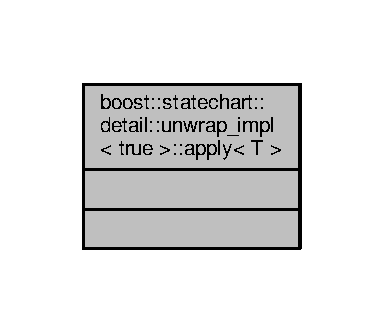
\includegraphics[width=184pt]{structboost_1_1statechart_1_1detail_1_1unwrap__impl_3_01true_01_4_1_1apply__coll__graph}
\end{center}
\end{figure}
\subsection*{Public Types}
\begin{DoxyCompactItemize}
\item 
typedef T\+::type \& \mbox{\hyperlink{structboost_1_1statechart_1_1detail_1_1unwrap__impl_3_01true_01_4_1_1apply_a780f1b70daae566b269900bd6aa0126c}{type}}
\end{DoxyCompactItemize}


\subsection{Member Typedef Documentation}
\mbox{\Hypertarget{structboost_1_1statechart_1_1detail_1_1unwrap__impl_3_01true_01_4_1_1apply_a780f1b70daae566b269900bd6aa0126c}\label{structboost_1_1statechart_1_1detail_1_1unwrap__impl_3_01true_01_4_1_1apply_a780f1b70daae566b269900bd6aa0126c}} 
\index{boost\+::statechart\+::detail\+::unwrap\+\_\+impl$<$ true $>$\+::apply@{boost\+::statechart\+::detail\+::unwrap\+\_\+impl$<$ true $>$\+::apply}!type@{type}}
\index{type@{type}!boost\+::statechart\+::detail\+::unwrap\+\_\+impl$<$ true $>$\+::apply@{boost\+::statechart\+::detail\+::unwrap\+\_\+impl$<$ true $>$\+::apply}}
\subsubsection{\texorpdfstring{type}{type}}
{\footnotesize\ttfamily template$<$typename T $>$ \\
typedef T\+::type\& \mbox{\hyperlink{structboost_1_1statechart_1_1detail_1_1unwrap__impl}{boost\+::statechart\+::detail\+::unwrap\+\_\+impl}}$<$ true $>$\+::apply$<$ T $>$\+::\mbox{\hyperlink{structboost_1_1statechart_1_1detail_1_1unwrap__impl_3_01true_01_4_1_1apply_a780f1b70daae566b269900bd6aa0126c}{type}}}



The documentation for this struct was generated from the following file\+:\begin{DoxyCompactItemize}
\item 
include/boost/statechart/\mbox{\hyperlink{processor__container_8hpp}{processor\+\_\+container.\+hpp}}\end{DoxyCompactItemize}

\hypertarget{classboost_1_1statechart_1_1asynchronous__state__machine}{}\section{boost\+:\+:statechart\+:\+:asynchronous\+\_\+state\+\_\+machine$<$ Most\+Derived, Initial\+State, Scheduler, Allocator, Exception\+Translator $>$ Class Template Reference}
\label{classboost_1_1statechart_1_1asynchronous__state__machine}\index{boost\+::statechart\+::asynchronous\+\_\+state\+\_\+machine$<$ Most\+Derived, Initial\+State, Scheduler, Allocator, Exception\+Translator $>$@{boost\+::statechart\+::asynchronous\+\_\+state\+\_\+machine$<$ Most\+Derived, Initial\+State, Scheduler, Allocator, Exception\+Translator $>$}}


{\ttfamily \#include $<$asynchronous\+\_\+state\+\_\+machine.\+hpp$>$}



Inheritance diagram for boost\+:\+:statechart\+:\+:asynchronous\+\_\+state\+\_\+machine$<$ Most\+Derived, Initial\+State, Scheduler, Allocator, Exception\+Translator $>$\+:
\nopagebreak
\begin{figure}[H]
\begin{center}
\leavevmode
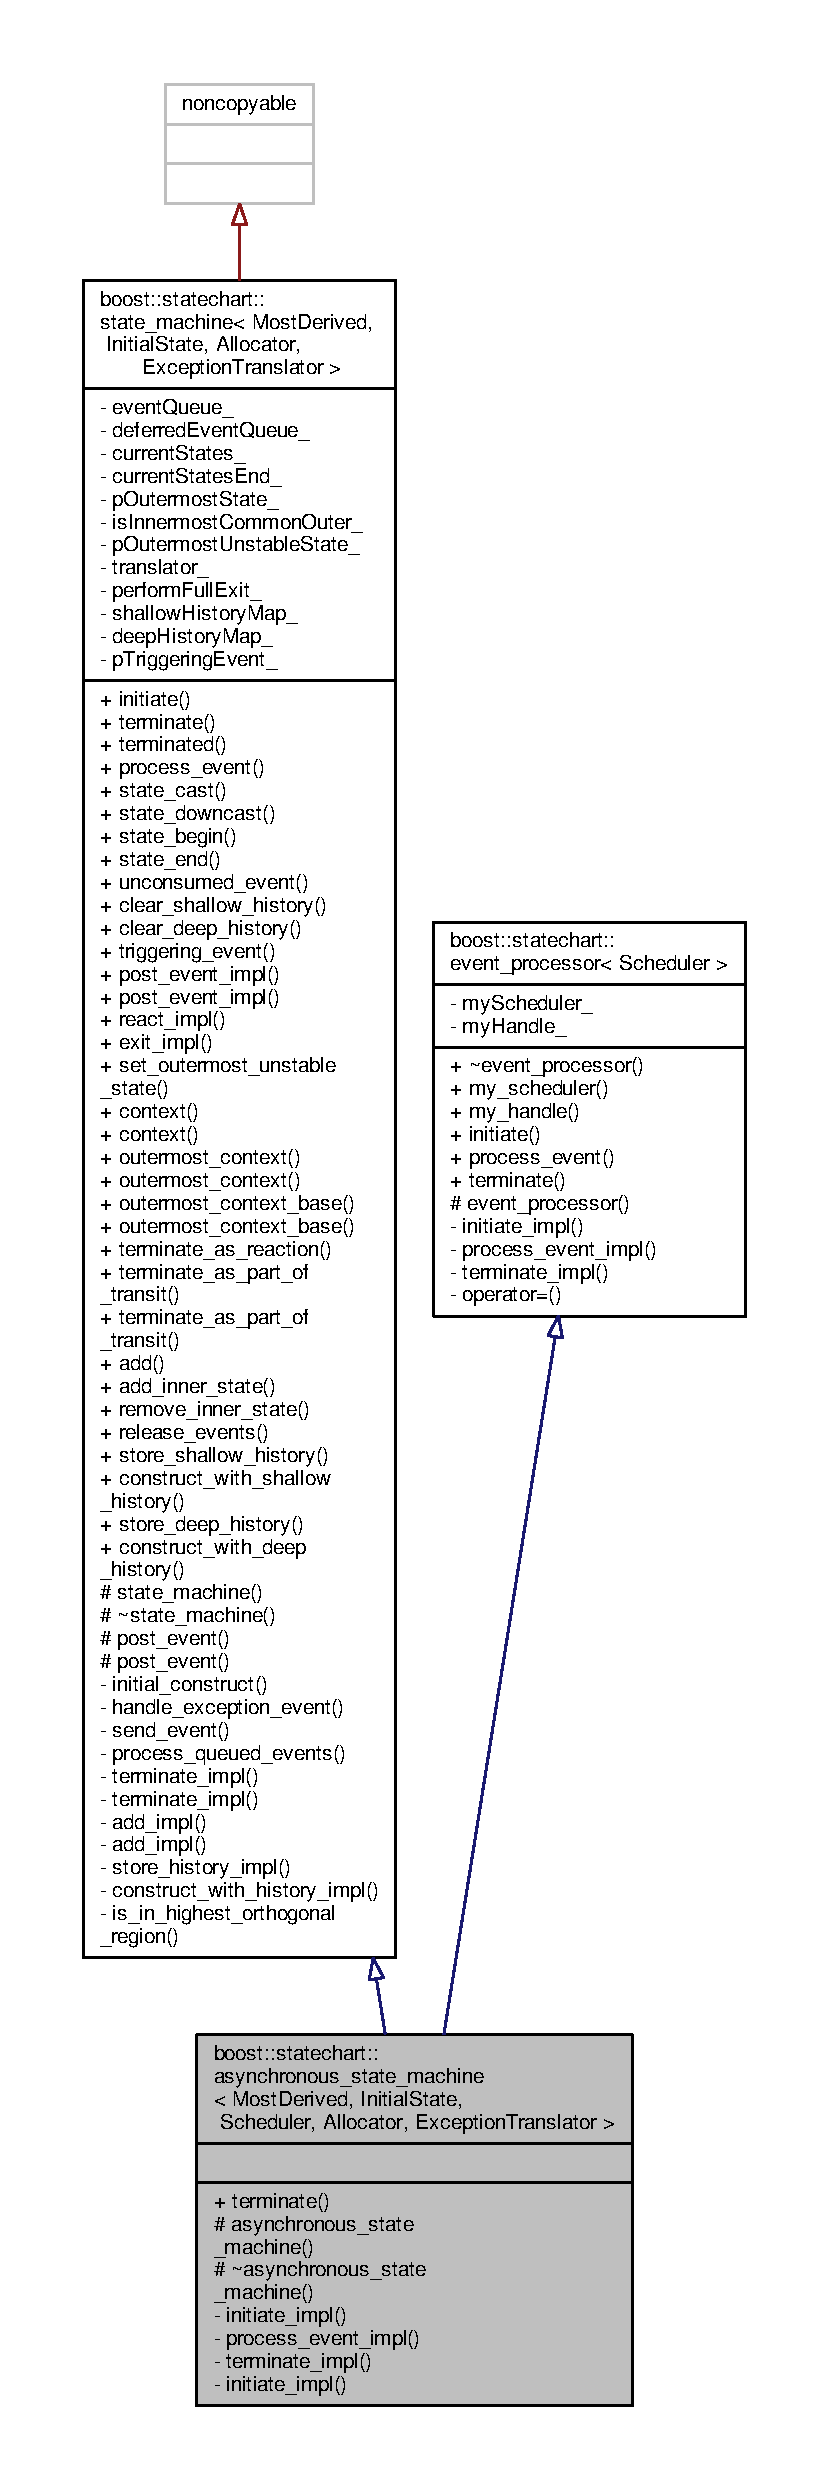
\includegraphics[height=550pt]{classboost_1_1statechart_1_1asynchronous__state__machine__inherit__graph}
\end{center}
\end{figure}


Collaboration diagram for boost\+:\+:statechart\+:\+:asynchronous\+\_\+state\+\_\+machine$<$ Most\+Derived, Initial\+State, Scheduler, Allocator, Exception\+Translator $>$\+:
\nopagebreak
\begin{figure}[H]
\begin{center}
\leavevmode
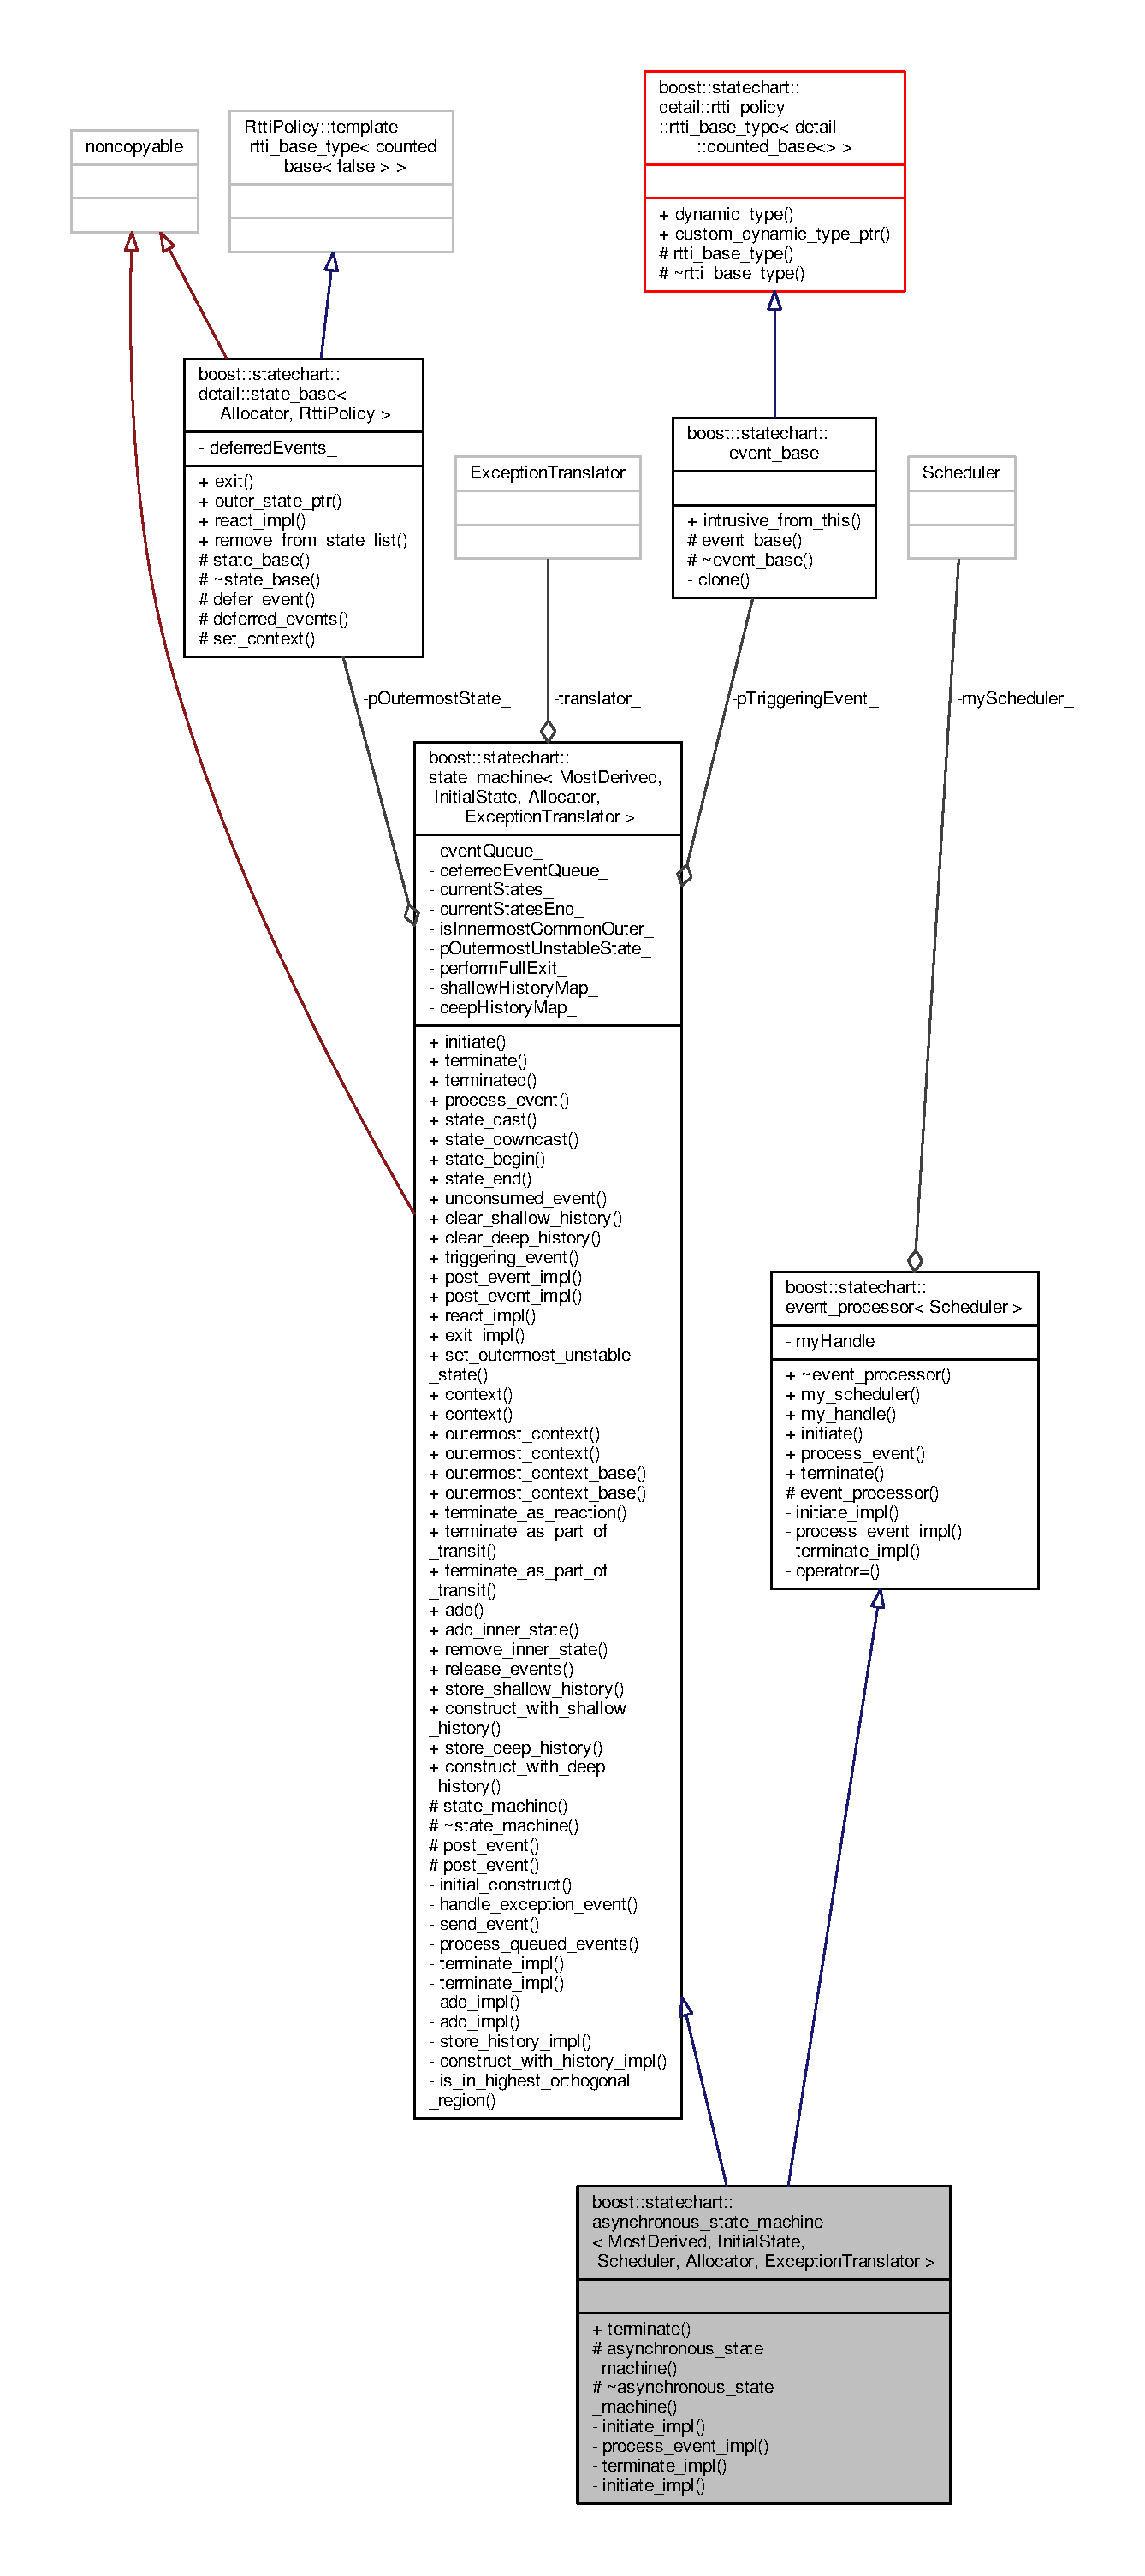
\includegraphics[height=550pt]{classboost_1_1statechart_1_1asynchronous__state__machine__coll__graph}
\end{center}
\end{figure}
\subsection*{Public Member Functions}
\begin{DoxyCompactItemize}
\item 
void \mbox{\hyperlink{classboost_1_1statechart_1_1asynchronous__state__machine_aeb5ac2e3a0f539b313544357ae2be26d}{terminate}} ()
\end{DoxyCompactItemize}
\subsection*{Protected Types}
\begin{DoxyCompactItemize}
\item 
typedef \mbox{\hyperlink{classboost_1_1statechart_1_1asynchronous__state__machine}{asynchronous\+\_\+state\+\_\+machine}} \mbox{\hyperlink{classboost_1_1statechart_1_1asynchronous__state__machine_ad2d3eb216740758af0982c1b04e7331d}{my\+\_\+base}}
\end{DoxyCompactItemize}
\subsection*{Protected Member Functions}
\begin{DoxyCompactItemize}
\item 
\mbox{\hyperlink{classboost_1_1statechart_1_1asynchronous__state__machine_af27bb28945bb6a4d824e3a2c0a7c6968}{asynchronous\+\_\+state\+\_\+machine}} (typename \mbox{\hyperlink{classboost_1_1statechart_1_1event__processor_a99f1c6ec8419ec82f140c5c93c5eb8cd}{processor\+\_\+base\+::my\+\_\+context}} ctx)
\item 
virtual \mbox{\hyperlink{classboost_1_1statechart_1_1asynchronous__state__machine_aca67fcba8555b76db8c1d13c94f597bb}{$\sim$asynchronous\+\_\+state\+\_\+machine}} ()
\end{DoxyCompactItemize}
\subsection*{Private Types}
\begin{DoxyCompactItemize}
\item 
typedef \mbox{\hyperlink{classboost_1_1statechart_1_1state__machine}{state\+\_\+machine}}$<$ Most\+Derived, Initial\+State, Allocator, Exception\+Translator $>$ \mbox{\hyperlink{classboost_1_1statechart_1_1asynchronous__state__machine_a5fb2caf90c443b6517ecb6ce86a672d7}{machine\+\_\+base}}
\item 
typedef \mbox{\hyperlink{classboost_1_1statechart_1_1event__processor}{event\+\_\+processor}}$<$ Scheduler $>$ \mbox{\hyperlink{classboost_1_1statechart_1_1asynchronous__state__machine_a59f192af18b9070396e42994a8dbeb35}{processor\+\_\+base}}
\end{DoxyCompactItemize}
\subsection*{Private Member Functions}
\begin{DoxyCompactItemize}
\item 
virtual void \mbox{\hyperlink{classboost_1_1statechart_1_1asynchronous__state__machine_a346bde99a27dc391a0c4beb8c728dce0}{initiate\+\_\+impl}} ()
\item 
virtual void \mbox{\hyperlink{classboost_1_1statechart_1_1asynchronous__state__machine_a3e4a4a8910ec610542fc41dba4fd2d04}{process\+\_\+event\+\_\+impl}} (const \mbox{\hyperlink{classboost_1_1statechart_1_1event__base}{event\+\_\+base}} \&evt)
\item 
virtual void \mbox{\hyperlink{classboost_1_1statechart_1_1asynchronous__state__machine_a528bedaf8c4d4b3fefc78984673bf30b}{terminate\+\_\+impl}} ()
\item 
{\footnotesize template$<$$>$ }\\void \mbox{\hyperlink{classboost_1_1statechart_1_1asynchronous__state__machine_a7c4de22b056f8a85f2c163b6c5677f23}{initiate\+\_\+impl}} ()
\end{DoxyCompactItemize}
\subsection*{Additional Inherited Members}


\subsection{Member Typedef Documentation}
\mbox{\Hypertarget{classboost_1_1statechart_1_1asynchronous__state__machine_a5fb2caf90c443b6517ecb6ce86a672d7}\label{classboost_1_1statechart_1_1asynchronous__state__machine_a5fb2caf90c443b6517ecb6ce86a672d7}} 
\index{boost\+::statechart\+::asynchronous\+\_\+state\+\_\+machine@{boost\+::statechart\+::asynchronous\+\_\+state\+\_\+machine}!machine\+\_\+base@{machine\+\_\+base}}
\index{machine\+\_\+base@{machine\+\_\+base}!boost\+::statechart\+::asynchronous\+\_\+state\+\_\+machine@{boost\+::statechart\+::asynchronous\+\_\+state\+\_\+machine}}
\subsubsection{\texorpdfstring{machine\+\_\+base}{machine\_base}}
{\footnotesize\ttfamily template$<$class Most\+Derived, class Initial\+State, class Scheduler = fifo\+\_\+scheduler$<$$>$, class Allocator = std\+::allocator$<$ void $>$, class Exception\+Translator = null\+\_\+exception\+\_\+translator$>$ \\
typedef \mbox{\hyperlink{classboost_1_1statechart_1_1state__machine}{state\+\_\+machine}}$<$ Most\+Derived, Initial\+State, Allocator, Exception\+Translator $>$ \mbox{\hyperlink{classboost_1_1statechart_1_1asynchronous__state__machine}{boost\+::statechart\+::asynchronous\+\_\+state\+\_\+machine}}$<$ Most\+Derived, Initial\+State, Scheduler, Allocator, Exception\+Translator $>$\+::\mbox{\hyperlink{classboost_1_1statechart_1_1asynchronous__state__machine_a5fb2caf90c443b6517ecb6ce86a672d7}{machine\+\_\+base}}\hspace{0.3cm}{\ttfamily [private]}}

\mbox{\Hypertarget{classboost_1_1statechart_1_1asynchronous__state__machine_ad2d3eb216740758af0982c1b04e7331d}\label{classboost_1_1statechart_1_1asynchronous__state__machine_ad2d3eb216740758af0982c1b04e7331d}} 
\index{boost\+::statechart\+::asynchronous\+\_\+state\+\_\+machine@{boost\+::statechart\+::asynchronous\+\_\+state\+\_\+machine}!my\+\_\+base@{my\+\_\+base}}
\index{my\+\_\+base@{my\+\_\+base}!boost\+::statechart\+::asynchronous\+\_\+state\+\_\+machine@{boost\+::statechart\+::asynchronous\+\_\+state\+\_\+machine}}
\subsubsection{\texorpdfstring{my\+\_\+base}{my\_base}}
{\footnotesize\ttfamily template$<$class Most\+Derived, class Initial\+State, class Scheduler = fifo\+\_\+scheduler$<$$>$, class Allocator = std\+::allocator$<$ void $>$, class Exception\+Translator = null\+\_\+exception\+\_\+translator$>$ \\
typedef \mbox{\hyperlink{classboost_1_1statechart_1_1asynchronous__state__machine}{asynchronous\+\_\+state\+\_\+machine}} \mbox{\hyperlink{classboost_1_1statechart_1_1asynchronous__state__machine}{boost\+::statechart\+::asynchronous\+\_\+state\+\_\+machine}}$<$ Most\+Derived, Initial\+State, Scheduler, Allocator, Exception\+Translator $>$\+::\mbox{\hyperlink{classboost_1_1statechart_1_1asynchronous__state__machine_ad2d3eb216740758af0982c1b04e7331d}{my\+\_\+base}}\hspace{0.3cm}{\ttfamily [protected]}}

\mbox{\Hypertarget{classboost_1_1statechart_1_1asynchronous__state__machine_a59f192af18b9070396e42994a8dbeb35}\label{classboost_1_1statechart_1_1asynchronous__state__machine_a59f192af18b9070396e42994a8dbeb35}} 
\index{boost\+::statechart\+::asynchronous\+\_\+state\+\_\+machine@{boost\+::statechart\+::asynchronous\+\_\+state\+\_\+machine}!processor\+\_\+base@{processor\+\_\+base}}
\index{processor\+\_\+base@{processor\+\_\+base}!boost\+::statechart\+::asynchronous\+\_\+state\+\_\+machine@{boost\+::statechart\+::asynchronous\+\_\+state\+\_\+machine}}
\subsubsection{\texorpdfstring{processor\+\_\+base}{processor\_base}}
{\footnotesize\ttfamily template$<$class Most\+Derived, class Initial\+State, class Scheduler = fifo\+\_\+scheduler$<$$>$, class Allocator = std\+::allocator$<$ void $>$, class Exception\+Translator = null\+\_\+exception\+\_\+translator$>$ \\
typedef \mbox{\hyperlink{classboost_1_1statechart_1_1event__processor}{event\+\_\+processor}}$<$ Scheduler $>$ \mbox{\hyperlink{classboost_1_1statechart_1_1asynchronous__state__machine}{boost\+::statechart\+::asynchronous\+\_\+state\+\_\+machine}}$<$ Most\+Derived, Initial\+State, Scheduler, Allocator, Exception\+Translator $>$\+::\mbox{\hyperlink{classboost_1_1statechart_1_1asynchronous__state__machine_a59f192af18b9070396e42994a8dbeb35}{processor\+\_\+base}}\hspace{0.3cm}{\ttfamily [private]}}



\subsection{Constructor \& Destructor Documentation}
\mbox{\Hypertarget{classboost_1_1statechart_1_1asynchronous__state__machine_af27bb28945bb6a4d824e3a2c0a7c6968}\label{classboost_1_1statechart_1_1asynchronous__state__machine_af27bb28945bb6a4d824e3a2c0a7c6968}} 
\index{boost\+::statechart\+::asynchronous\+\_\+state\+\_\+machine@{boost\+::statechart\+::asynchronous\+\_\+state\+\_\+machine}!asynchronous\+\_\+state\+\_\+machine@{asynchronous\+\_\+state\+\_\+machine}}
\index{asynchronous\+\_\+state\+\_\+machine@{asynchronous\+\_\+state\+\_\+machine}!boost\+::statechart\+::asynchronous\+\_\+state\+\_\+machine@{boost\+::statechart\+::asynchronous\+\_\+state\+\_\+machine}}
\subsubsection{\texorpdfstring{asynchronous\+\_\+state\+\_\+machine()}{asynchronous\_state\_machine()}}
{\footnotesize\ttfamily template$<$class Most\+Derived, class Initial\+State, class Scheduler = fifo\+\_\+scheduler$<$$>$, class Allocator = std\+::allocator$<$ void $>$, class Exception\+Translator = null\+\_\+exception\+\_\+translator$>$ \\
\mbox{\hyperlink{classboost_1_1statechart_1_1asynchronous__state__machine}{boost\+::statechart\+::asynchronous\+\_\+state\+\_\+machine}}$<$ Most\+Derived, Initial\+State, Scheduler, Allocator, Exception\+Translator $>$\+::\mbox{\hyperlink{classboost_1_1statechart_1_1asynchronous__state__machine}{asynchronous\+\_\+state\+\_\+machine}} (\begin{DoxyParamCaption}\item[{typename \mbox{\hyperlink{classboost_1_1statechart_1_1event__processor_a99f1c6ec8419ec82f140c5c93c5eb8cd}{processor\+\_\+base\+::my\+\_\+context}}}]{ctx }\end{DoxyParamCaption})\hspace{0.3cm}{\ttfamily [inline]}, {\ttfamily [protected]}}

\mbox{\Hypertarget{classboost_1_1statechart_1_1asynchronous__state__machine_aca67fcba8555b76db8c1d13c94f597bb}\label{classboost_1_1statechart_1_1asynchronous__state__machine_aca67fcba8555b76db8c1d13c94f597bb}} 
\index{boost\+::statechart\+::asynchronous\+\_\+state\+\_\+machine@{boost\+::statechart\+::asynchronous\+\_\+state\+\_\+machine}!````~asynchronous\+\_\+state\+\_\+machine@{$\sim$asynchronous\+\_\+state\+\_\+machine}}
\index{````~asynchronous\+\_\+state\+\_\+machine@{$\sim$asynchronous\+\_\+state\+\_\+machine}!boost\+::statechart\+::asynchronous\+\_\+state\+\_\+machine@{boost\+::statechart\+::asynchronous\+\_\+state\+\_\+machine}}
\subsubsection{\texorpdfstring{$\sim$asynchronous\+\_\+state\+\_\+machine()}{~asynchronous\_state\_machine()}}
{\footnotesize\ttfamily template$<$class Most\+Derived, class Initial\+State, class Scheduler = fifo\+\_\+scheduler$<$$>$, class Allocator = std\+::allocator$<$ void $>$, class Exception\+Translator = null\+\_\+exception\+\_\+translator$>$ \\
virtual \mbox{\hyperlink{classboost_1_1statechart_1_1asynchronous__state__machine}{boost\+::statechart\+::asynchronous\+\_\+state\+\_\+machine}}$<$ Most\+Derived, Initial\+State, Scheduler, Allocator, Exception\+Translator $>$\+::$\sim$\mbox{\hyperlink{classboost_1_1statechart_1_1asynchronous__state__machine}{asynchronous\+\_\+state\+\_\+machine}} (\begin{DoxyParamCaption}{ }\end{DoxyParamCaption})\hspace{0.3cm}{\ttfamily [inline]}, {\ttfamily [protected]}, {\ttfamily [virtual]}}



\subsection{Member Function Documentation}
\mbox{\Hypertarget{classboost_1_1statechart_1_1asynchronous__state__machine_a346bde99a27dc391a0c4beb8c728dce0}\label{classboost_1_1statechart_1_1asynchronous__state__machine_a346bde99a27dc391a0c4beb8c728dce0}} 
\index{boost\+::statechart\+::asynchronous\+\_\+state\+\_\+machine@{boost\+::statechart\+::asynchronous\+\_\+state\+\_\+machine}!initiate\+\_\+impl@{initiate\+\_\+impl}}
\index{initiate\+\_\+impl@{initiate\+\_\+impl}!boost\+::statechart\+::asynchronous\+\_\+state\+\_\+machine@{boost\+::statechart\+::asynchronous\+\_\+state\+\_\+machine}}
\subsubsection{\texorpdfstring{initiate\+\_\+impl()}{initiate\_impl()}\hspace{0.1cm}{\footnotesize\ttfamily [1/2]}}
{\footnotesize\ttfamily template$<$class Most\+Derived, class Initial\+State, class Scheduler = fifo\+\_\+scheduler$<$$>$, class Allocator = std\+::allocator$<$ void $>$, class Exception\+Translator = null\+\_\+exception\+\_\+translator$>$ \\
virtual void \mbox{\hyperlink{classboost_1_1statechart_1_1asynchronous__state__machine}{boost\+::statechart\+::asynchronous\+\_\+state\+\_\+machine}}$<$ Most\+Derived, Initial\+State, Scheduler, Allocator, Exception\+Translator $>$\+::initiate\+\_\+impl (\begin{DoxyParamCaption}{ }\end{DoxyParamCaption})\hspace{0.3cm}{\ttfamily [inline]}, {\ttfamily [private]}, {\ttfamily [virtual]}}



Implements \mbox{\hyperlink{classboost_1_1statechart_1_1event__processor_a48a2bfcad66582f6c88e6034b2b838cb}{boost\+::statechart\+::event\+\_\+processor$<$ Scheduler $>$}}.



Reimplemented in \mbox{\hyperlink{struct_player_ae5001b1a7c1ba022d7bdb6d7da25e647}{Player}}.

\mbox{\Hypertarget{classboost_1_1statechart_1_1asynchronous__state__machine_a7c4de22b056f8a85f2c163b6c5677f23}\label{classboost_1_1statechart_1_1asynchronous__state__machine_a7c4de22b056f8a85f2c163b6c5677f23}} 
\index{boost\+::statechart\+::asynchronous\+\_\+state\+\_\+machine@{boost\+::statechart\+::asynchronous\+\_\+state\+\_\+machine}!initiate\+\_\+impl@{initiate\+\_\+impl}}
\index{initiate\+\_\+impl@{initiate\+\_\+impl}!boost\+::statechart\+::asynchronous\+\_\+state\+\_\+machine@{boost\+::statechart\+::asynchronous\+\_\+state\+\_\+machine}}
\subsubsection{\texorpdfstring{initiate\+\_\+impl()}{initiate\_impl()}\hspace{0.1cm}{\footnotesize\ttfamily [2/2]}}
{\footnotesize\ttfamily template$<$$>$ \\
void \mbox{\hyperlink{classboost_1_1statechart_1_1asynchronous__state__machine}{boost\+::statechart\+::asynchronous\+\_\+state\+\_\+machine}}$<$ \mbox{\hyperlink{struct_player}{Player}}, \mbox{\hyperlink{struct_waiting}{Waiting}}, \mbox{\hyperlink{_player_8hpp_a24a1f41c11f96c5934bd8e82b4fb2805}{My\+Scheduler}}, \mbox{\hyperlink{_player_8hpp_ab302cdbc6b094291e393ac49d404d75a}{My\+Allocator}} $>$\+::initiate\+\_\+impl (\begin{DoxyParamCaption}{ }\end{DoxyParamCaption})\hspace{0.3cm}{\ttfamily [inline]}, {\ttfamily [private]}, {\ttfamily [virtual]}}



Implements \mbox{\hyperlink{classboost_1_1statechart_1_1event__processor_a48a2bfcad66582f6c88e6034b2b838cb}{boost\+::statechart\+::event\+\_\+processor$<$ Scheduler $>$}}.

\mbox{\Hypertarget{classboost_1_1statechart_1_1asynchronous__state__machine_a3e4a4a8910ec610542fc41dba4fd2d04}\label{classboost_1_1statechart_1_1asynchronous__state__machine_a3e4a4a8910ec610542fc41dba4fd2d04}} 
\index{boost\+::statechart\+::asynchronous\+\_\+state\+\_\+machine@{boost\+::statechart\+::asynchronous\+\_\+state\+\_\+machine}!process\+\_\+event\+\_\+impl@{process\+\_\+event\+\_\+impl}}
\index{process\+\_\+event\+\_\+impl@{process\+\_\+event\+\_\+impl}!boost\+::statechart\+::asynchronous\+\_\+state\+\_\+machine@{boost\+::statechart\+::asynchronous\+\_\+state\+\_\+machine}}
\subsubsection{\texorpdfstring{process\+\_\+event\+\_\+impl()}{process\_event\_impl()}}
{\footnotesize\ttfamily template$<$class Most\+Derived, class Initial\+State, class Scheduler = fifo\+\_\+scheduler$<$$>$, class Allocator = std\+::allocator$<$ void $>$, class Exception\+Translator = null\+\_\+exception\+\_\+translator$>$ \\
virtual void \mbox{\hyperlink{classboost_1_1statechart_1_1asynchronous__state__machine}{boost\+::statechart\+::asynchronous\+\_\+state\+\_\+machine}}$<$ Most\+Derived, Initial\+State, Scheduler, Allocator, Exception\+Translator $>$\+::process\+\_\+event\+\_\+impl (\begin{DoxyParamCaption}\item[{const \mbox{\hyperlink{classboost_1_1statechart_1_1event__base}{event\+\_\+base}} \&}]{evt }\end{DoxyParamCaption})\hspace{0.3cm}{\ttfamily [inline]}, {\ttfamily [private]}, {\ttfamily [virtual]}}



Implements \mbox{\hyperlink{classboost_1_1statechart_1_1event__processor_a5db03beb4d6c1545e7bb9584cd60b500}{boost\+::statechart\+::event\+\_\+processor$<$ Scheduler $>$}}.

\mbox{\Hypertarget{classboost_1_1statechart_1_1asynchronous__state__machine_aeb5ac2e3a0f539b313544357ae2be26d}\label{classboost_1_1statechart_1_1asynchronous__state__machine_aeb5ac2e3a0f539b313544357ae2be26d}} 
\index{boost\+::statechart\+::asynchronous\+\_\+state\+\_\+machine@{boost\+::statechart\+::asynchronous\+\_\+state\+\_\+machine}!terminate@{terminate}}
\index{terminate@{terminate}!boost\+::statechart\+::asynchronous\+\_\+state\+\_\+machine@{boost\+::statechart\+::asynchronous\+\_\+state\+\_\+machine}}
\subsubsection{\texorpdfstring{terminate()}{terminate()}}
{\footnotesize\ttfamily template$<$class Most\+Derived, class Initial\+State, class Scheduler = fifo\+\_\+scheduler$<$$>$, class Allocator = std\+::allocator$<$ void $>$, class Exception\+Translator = null\+\_\+exception\+\_\+translator$>$ \\
void \mbox{\hyperlink{classboost_1_1statechart_1_1asynchronous__state__machine}{boost\+::statechart\+::asynchronous\+\_\+state\+\_\+machine}}$<$ Most\+Derived, Initial\+State, Scheduler, Allocator, Exception\+Translator $>$\+::terminate (\begin{DoxyParamCaption}{ }\end{DoxyParamCaption})\hspace{0.3cm}{\ttfamily [inline]}}

\mbox{\Hypertarget{classboost_1_1statechart_1_1asynchronous__state__machine_a528bedaf8c4d4b3fefc78984673bf30b}\label{classboost_1_1statechart_1_1asynchronous__state__machine_a528bedaf8c4d4b3fefc78984673bf30b}} 
\index{boost\+::statechart\+::asynchronous\+\_\+state\+\_\+machine@{boost\+::statechart\+::asynchronous\+\_\+state\+\_\+machine}!terminate\+\_\+impl@{terminate\+\_\+impl}}
\index{terminate\+\_\+impl@{terminate\+\_\+impl}!boost\+::statechart\+::asynchronous\+\_\+state\+\_\+machine@{boost\+::statechart\+::asynchronous\+\_\+state\+\_\+machine}}
\subsubsection{\texorpdfstring{terminate\+\_\+impl()}{terminate\_impl()}}
{\footnotesize\ttfamily template$<$class Most\+Derived, class Initial\+State, class Scheduler = fifo\+\_\+scheduler$<$$>$, class Allocator = std\+::allocator$<$ void $>$, class Exception\+Translator = null\+\_\+exception\+\_\+translator$>$ \\
virtual void \mbox{\hyperlink{classboost_1_1statechart_1_1asynchronous__state__machine}{boost\+::statechart\+::asynchronous\+\_\+state\+\_\+machine}}$<$ Most\+Derived, Initial\+State, Scheduler, Allocator, Exception\+Translator $>$\+::terminate\+\_\+impl (\begin{DoxyParamCaption}{ }\end{DoxyParamCaption})\hspace{0.3cm}{\ttfamily [inline]}, {\ttfamily [private]}, {\ttfamily [virtual]}}



Implements \mbox{\hyperlink{classboost_1_1statechart_1_1event__processor_a3f5f4c757909fca5f389b485a789c24e}{boost\+::statechart\+::event\+\_\+processor$<$ Scheduler $>$}}.



The documentation for this class was generated from the following file\+:\begin{DoxyCompactItemize}
\item 
include/boost/statechart/\mbox{\hyperlink{asynchronous__state__machine_8hpp}{asynchronous\+\_\+state\+\_\+machine.\+hpp}}\end{DoxyCompactItemize}

\hypertarget{struct_b}{}\section{B Struct Reference}
\label{struct_b}\index{B@{B}}


Inheritance diagram for B\+:
\nopagebreak
\begin{figure}[H]
\begin{center}
\leavevmode
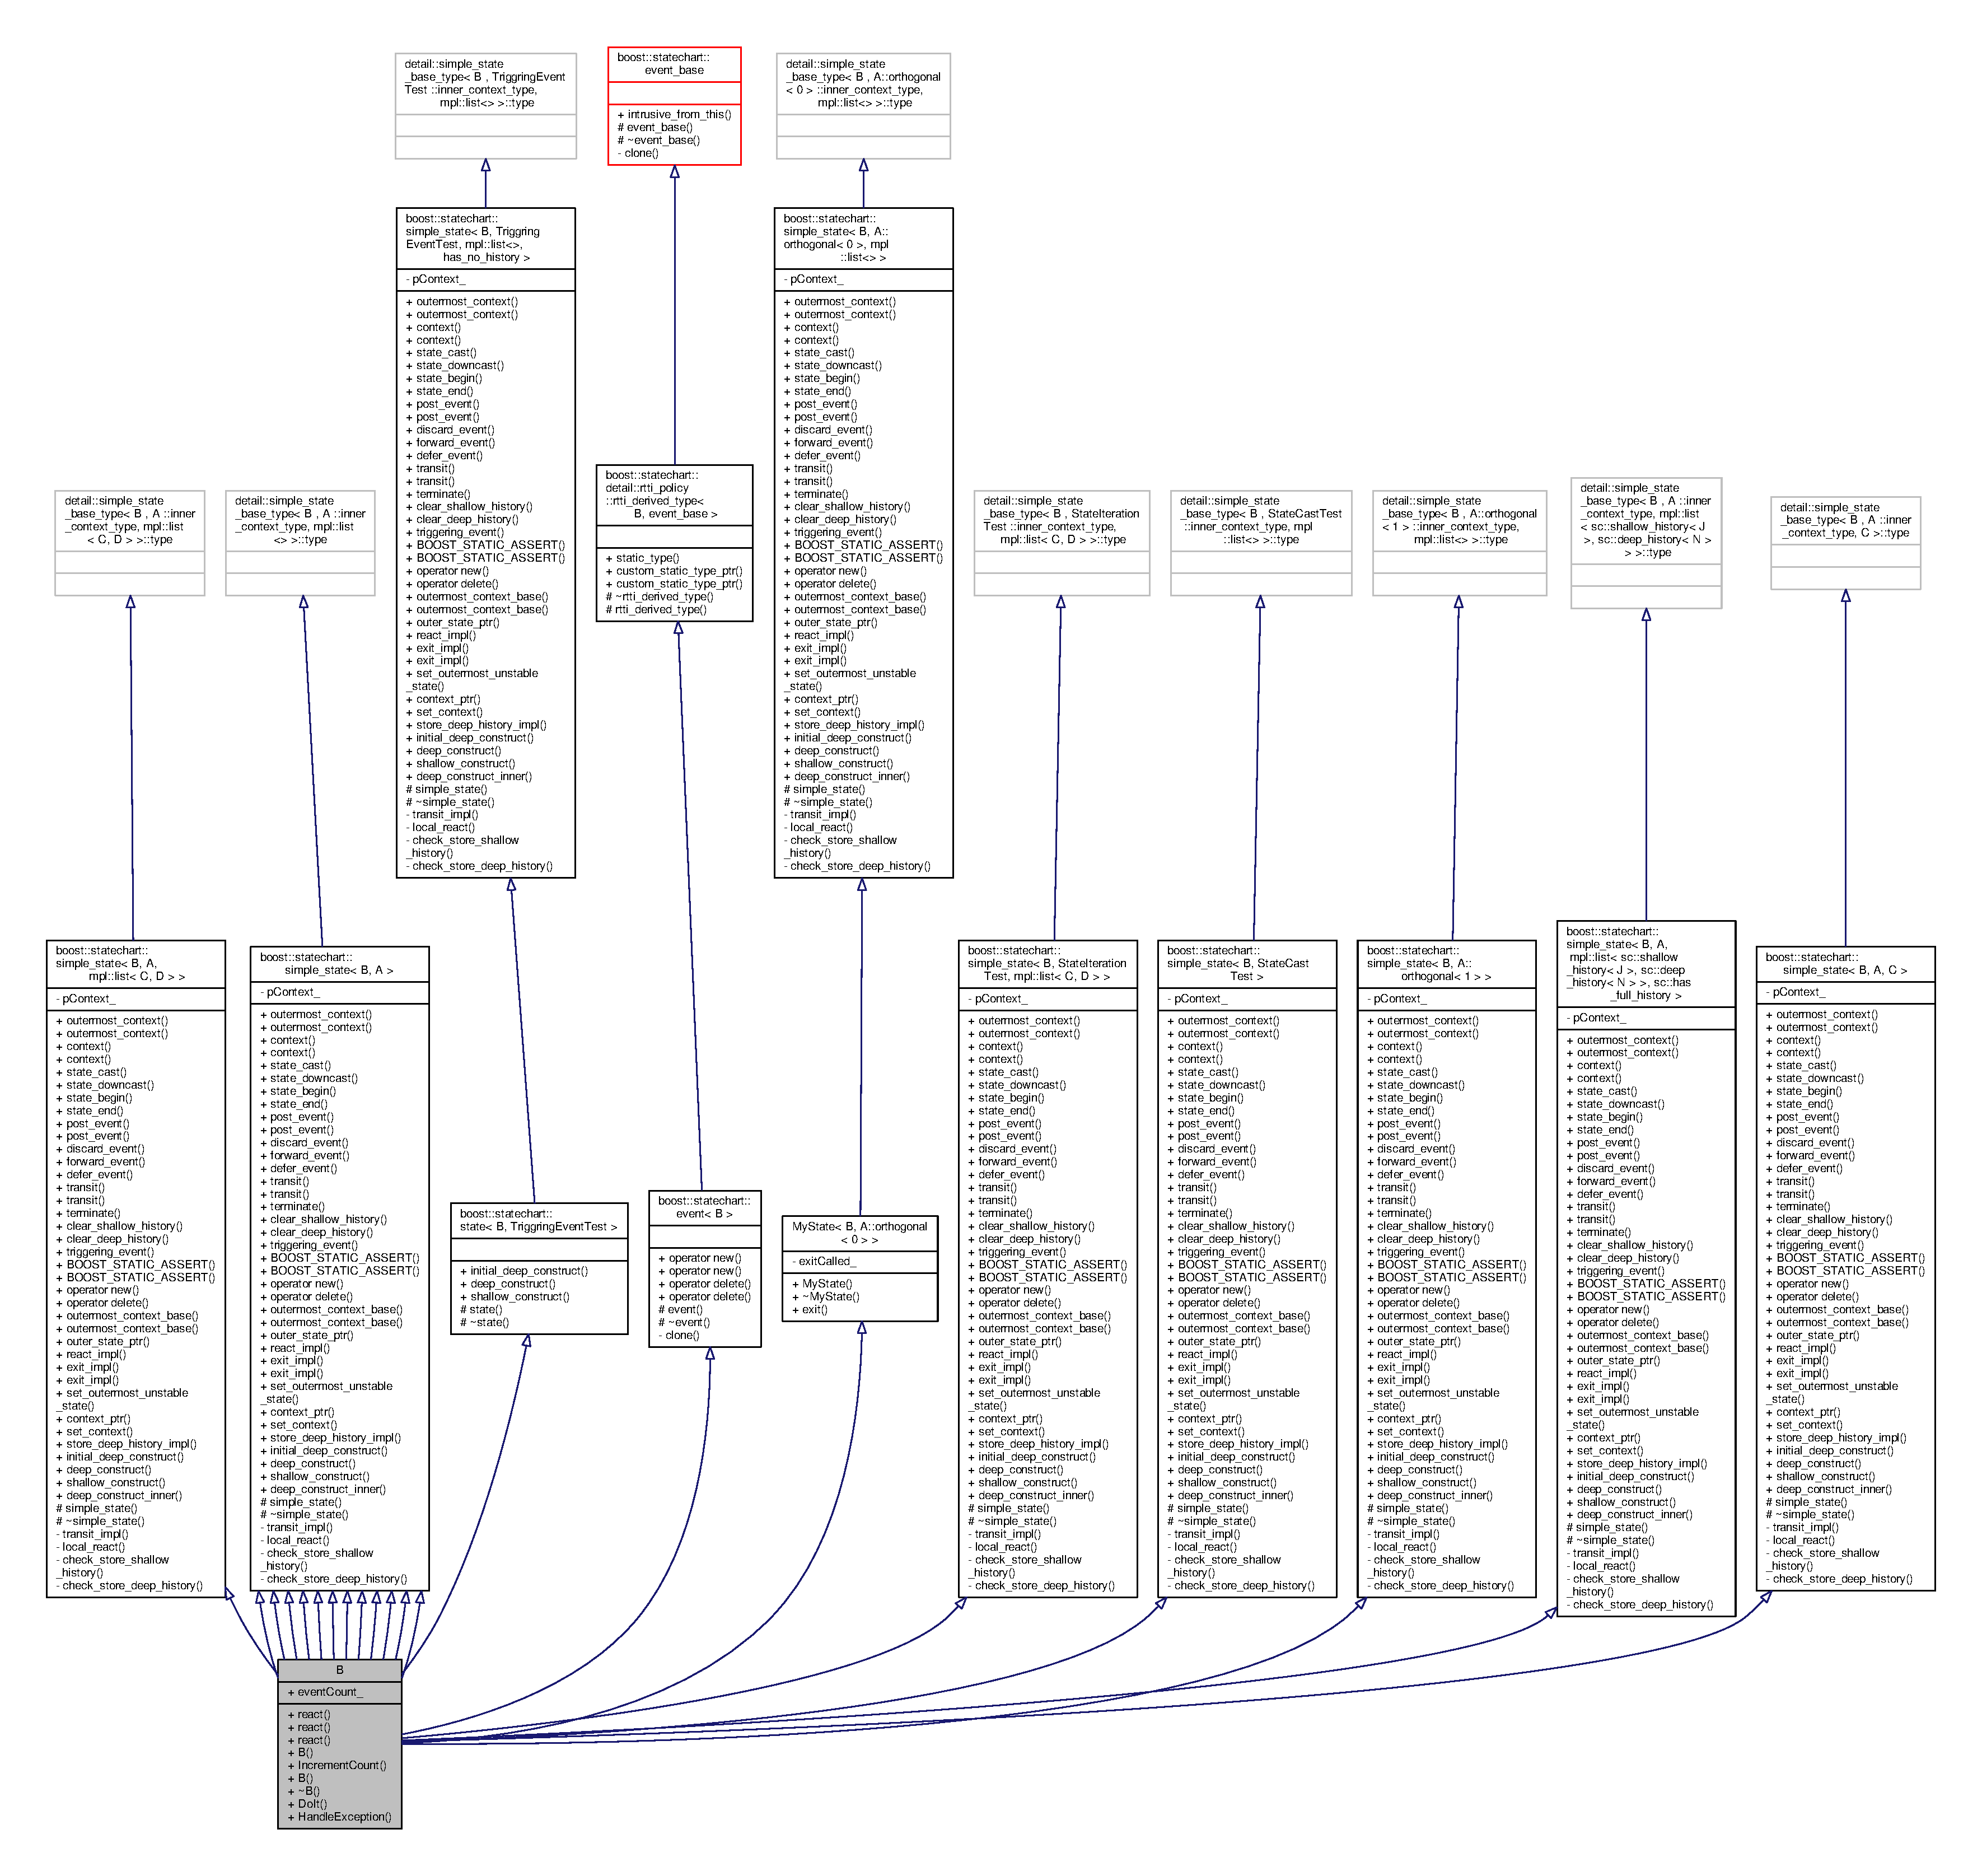
\includegraphics[width=350pt]{struct_b__inherit__graph}
\end{center}
\end{figure}


Collaboration diagram for B\+:
\nopagebreak
\begin{figure}[H]
\begin{center}
\leavevmode
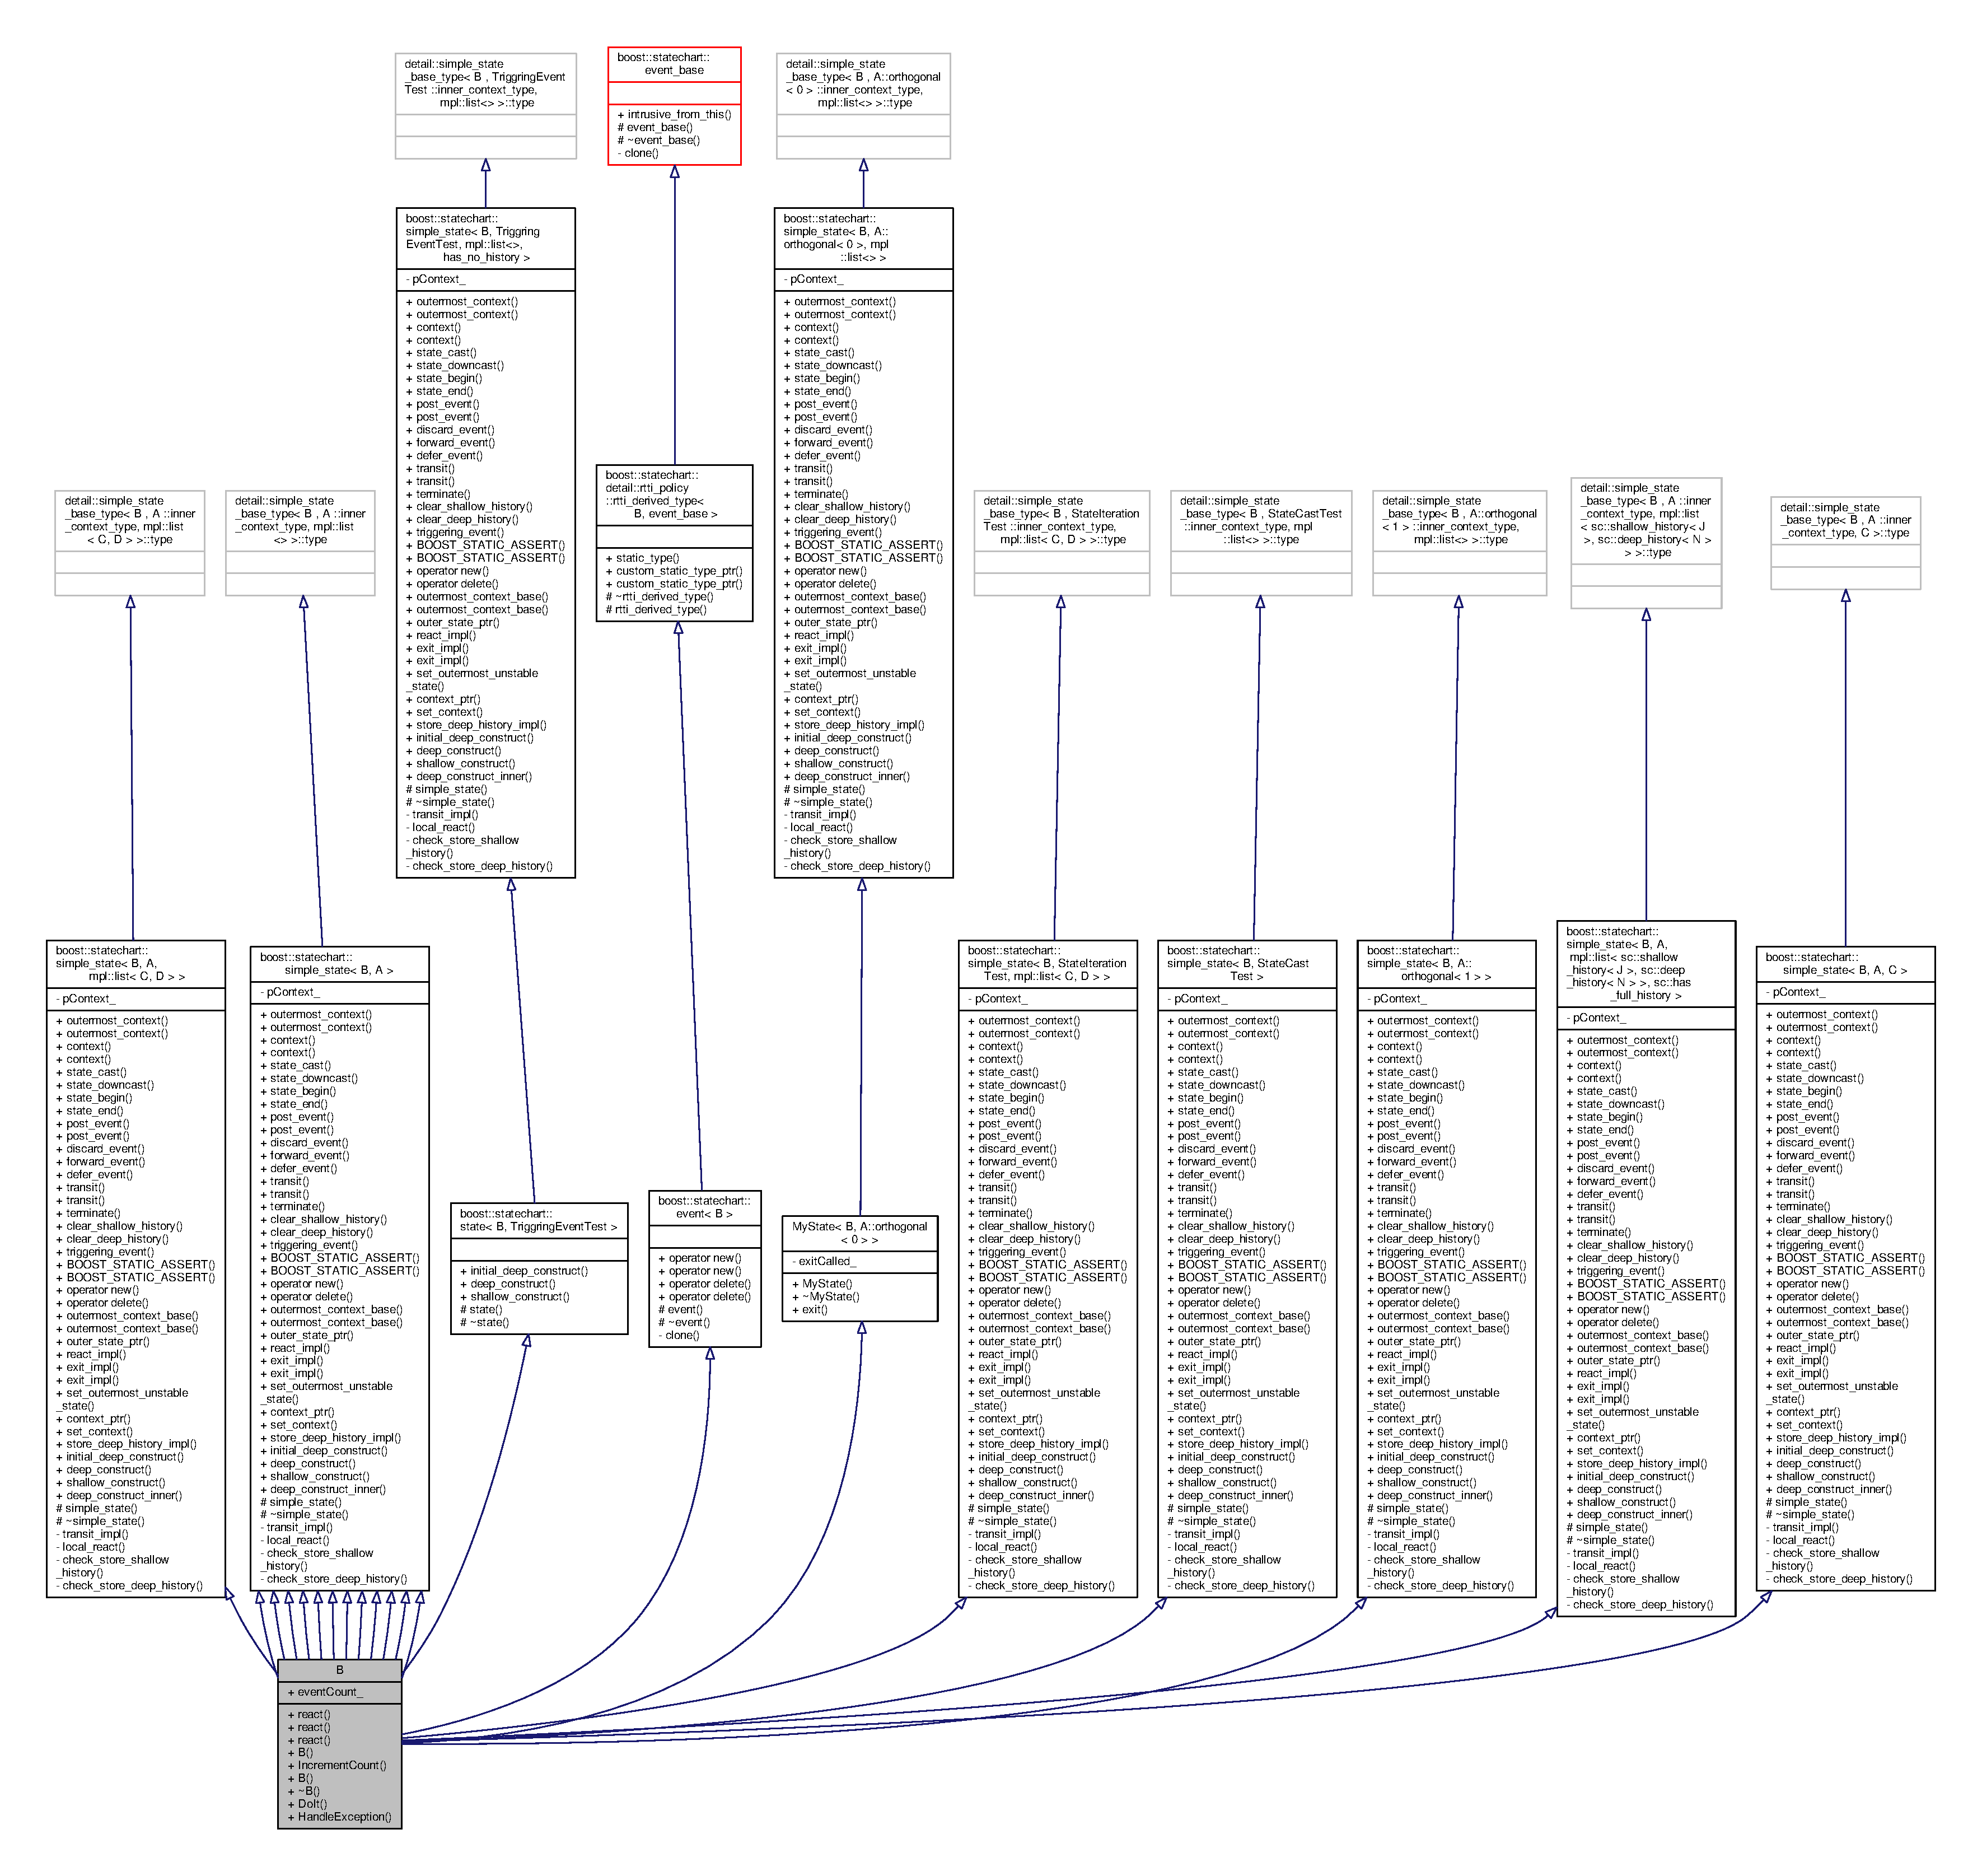
\includegraphics[width=350pt]{struct_b__coll__graph}
\end{center}
\end{figure}
\subsection*{Public Types}
\begin{DoxyCompactItemize}
\item 
typedef mpl\+::list$<$ \mbox{\hyperlink{classboost_1_1statechart_1_1custom__reaction}{sc\+::custom\+\_\+reaction}}$<$ \mbox{\hyperlink{struct_ev_discard_never}{Ev\+Discard\+Never}} $>$, \mbox{\hyperlink{classboost_1_1statechart_1_1custom__reaction}{sc\+::custom\+\_\+reaction}}$<$ \mbox{\hyperlink{struct_ev_discard_in_b}{Ev\+Discard\+InB}} $>$, \mbox{\hyperlink{classboost_1_1statechart_1_1custom__reaction}{sc\+::custom\+\_\+reaction}}$<$ \mbox{\hyperlink{struct_ev_discard_in_d}{Ev\+Discard\+InD}} $>$ $>$ \mbox{\hyperlink{struct_b_a2a510c568bd4f5254e154e713bcc7724}{reactions}}
\item 
typedef mpl\+::list$<$ \mbox{\hyperlink{classboost_1_1statechart_1_1in__state__reaction}{sc\+::in\+\_\+state\+\_\+reaction}}$<$ \mbox{\hyperlink{struct_f}{F}}, \mbox{\hyperlink{struct_b}{B}}, \&\mbox{\hyperlink{struct_b_a862e39288b607fcc7e71f9fa07c0cd20}{B\+::\+Increment\+Count}} $>$, \mbox{\hyperlink{classboost_1_1statechart_1_1in__state__reaction}{sc\+::in\+\_\+state\+\_\+reaction}}$<$ \mbox{\hyperlink{struct_g}{G}}, \mbox{\hyperlink{struct_a}{A}}, \&\mbox{\hyperlink{struct_a_a7811ed8883449fde0d5f59bd2ebf3de5}{A\+::\+Increment\+Count}} $>$, \mbox{\hyperlink{classboost_1_1statechart_1_1in__state__reaction}{sc\+::in\+\_\+state\+\_\+reaction}}$<$ \mbox{\hyperlink{struct_i}{I}} $>$ $>$ \mbox{\hyperlink{struct_b_a29fc5ace91a2e4f1854b15b8b301e458}{reactions}}
\item 
typedef \mbox{\hyperlink{classboost_1_1statechart_1_1transition}{sc\+::transition}}$<$ \mbox{\hyperlink{struct_ev_to_f}{Ev\+ToF}}, \mbox{\hyperlink{struct_f}{F}} $>$ \mbox{\hyperlink{struct_b_a0d7ad9cec2dd9d373b89c38a620756c0}{reactions}}
\item 
typedef \mbox{\hyperlink{classboost_1_1statechart_1_1transition}{sc\+::transition}}$<$ \mbox{\hyperlink{struct_ev_to_a}{Ev\+ToA}}, \mbox{\hyperlink{struct_a}{A}} $>$ \mbox{\hyperlink{struct_b_a3c296c27b9a29f5075166d4261902612}{reactions}}
\item 
typedef \mbox{\hyperlink{classboost_1_1statechart_1_1termination}{sc\+::termination}}$<$ \mbox{\hyperlink{struct_ev_terminate_b}{Ev\+TerminateB}} $>$ \mbox{\hyperlink{struct_b_a1ccdc4cf50c4df6bd758bb055b47dd01}{reactions}}
\item 
typedef mpl\+::list$<$ \mbox{\hyperlink{classboost_1_1statechart_1_1in__state__reaction}{sc\+::in\+\_\+state\+\_\+reaction}}$<$ \mbox{\hyperlink{struct_ev_do_it}{Ev\+Do\+It}}, \mbox{\hyperlink{struct_b}{B}}, \&\mbox{\hyperlink{struct_b_ad8417b0b86326962007c13d75094330e}{B\+::\+Do\+It}} $>$, \mbox{\hyperlink{classboost_1_1statechart_1_1in__state__reaction}{sc\+::in\+\_\+state\+\_\+reaction}}$<$ \mbox{\hyperlink{classboost_1_1statechart_1_1exception__thrown}{sc\+::exception\+\_\+thrown}}, \mbox{\hyperlink{struct_b}{B}}, \&\mbox{\hyperlink{struct_b_a8eb80df2fcfde5209e4800f5aec2d7a5}{B\+::\+Handle\+Exception}} $>$ $>$ \mbox{\hyperlink{struct_b_abbfe19dac6bb98dbb89c39caf2aa46d9}{reactions}}
\end{DoxyCompactItemize}
\subsection*{Public Member Functions}
\begin{DoxyCompactItemize}
\item 
\mbox{\hyperlink{namespaceboost_1_1statechart_abe807f6598b614d6d87bb951ecd92331}{sc\+::result}} \mbox{\hyperlink{struct_b_add69d6626a14cef8f58929dfbe940cb9}{react}} (const \mbox{\hyperlink{struct_ev_discard_never}{Ev\+Discard\+Never}} \&)
\item 
\mbox{\hyperlink{namespaceboost_1_1statechart_abe807f6598b614d6d87bb951ecd92331}{sc\+::result}} \mbox{\hyperlink{struct_b_af883c81d64b442ed4252a406a2710459}{react}} (const \mbox{\hyperlink{struct_ev_discard_in_b}{Ev\+Discard\+InB}} \&)
\item 
\mbox{\hyperlink{namespaceboost_1_1statechart_abe807f6598b614d6d87bb951ecd92331}{sc\+::result}} \mbox{\hyperlink{struct_b_a6ef8f2fd99e04b465b39ea65056ebc10}{react}} (const \mbox{\hyperlink{struct_ev_discard_in_d}{Ev\+Discard\+InD}} \&)
\item 
\mbox{\hyperlink{struct_b_a9532a74021f7efb003dffbc9d4145e65}{B}} ()
\item 
void \mbox{\hyperlink{struct_b_a862e39288b607fcc7e71f9fa07c0cd20}{Increment\+Count}} (const \mbox{\hyperlink{struct_f}{F}} \&)
\item 
\mbox{\hyperlink{struct_b_a8d6359453d0d6206098cf1980b6c7495}{B}} (my\+\_\+context ctx)
\item 
\mbox{\hyperlink{struct_b_abf3bb815dcba0116aee6f0e87d694702}{$\sim$B}} ()
\item 
void \mbox{\hyperlink{struct_b_ad8417b0b86326962007c13d75094330e}{Do\+It}} (const \mbox{\hyperlink{struct_ev_do_it}{Ev\+Do\+It}} \&)
\item 
void \mbox{\hyperlink{struct_b_a8eb80df2fcfde5209e4800f5aec2d7a5}{Handle\+Exception}} (const \mbox{\hyperlink{classboost_1_1statechart_1_1exception__thrown}{sc\+::exception\+\_\+thrown}} \&)
\end{DoxyCompactItemize}
\subsection*{Public Attributes}
\begin{DoxyCompactItemize}
\item 
unsigned int \mbox{\hyperlink{struct_b_a1a60275928b3599e275f5ba2c34b3a1b}{event\+Count\+\_\+}}
\end{DoxyCompactItemize}
\subsection*{Additional Inherited Members}


\subsection{Member Typedef Documentation}
\mbox{\Hypertarget{struct_b_a29fc5ace91a2e4f1854b15b8b301e458}\label{struct_b_a29fc5ace91a2e4f1854b15b8b301e458}} 
\index{B@{B}!reactions@{reactions}}
\index{reactions@{reactions}!B@{B}}
\subsubsection{\texorpdfstring{reactions}{reactions}\hspace{0.1cm}{\footnotesize\ttfamily [1/6]}}
{\footnotesize\ttfamily typedef mpl\+::list$<$ \mbox{\hyperlink{classboost_1_1statechart_1_1in__state__reaction}{sc\+::in\+\_\+state\+\_\+reaction}}$<$ \mbox{\hyperlink{struct_f}{F}}, \mbox{\hyperlink{struct_b}{B}}, \&\mbox{\hyperlink{struct_b_a862e39288b607fcc7e71f9fa07c0cd20}{B\+::\+Increment\+Count}} $>$, \mbox{\hyperlink{classboost_1_1statechart_1_1in__state__reaction}{sc\+::in\+\_\+state\+\_\+reaction}}$<$ \mbox{\hyperlink{struct_g}{G}}, \mbox{\hyperlink{struct_a}{A}}, \&\mbox{\hyperlink{struct_a_a7811ed8883449fde0d5f59bd2ebf3de5}{A\+::\+Increment\+Count}} $>$, \mbox{\hyperlink{classboost_1_1statechart_1_1in__state__reaction}{sc\+::in\+\_\+state\+\_\+reaction}}$<$ \mbox{\hyperlink{struct_i}{I}} $>$ $>$ \mbox{\hyperlink{struct_b_a2a510c568bd4f5254e154e713bcc7724}{B\+::reactions}}}

\mbox{\Hypertarget{struct_b_abbfe19dac6bb98dbb89c39caf2aa46d9}\label{struct_b_abbfe19dac6bb98dbb89c39caf2aa46d9}} 
\index{B@{B}!reactions@{reactions}}
\index{reactions@{reactions}!B@{B}}
\subsubsection{\texorpdfstring{reactions}{reactions}\hspace{0.1cm}{\footnotesize\ttfamily [2/6]}}
{\footnotesize\ttfamily typedef mpl\+::list$<$ \mbox{\hyperlink{classboost_1_1statechart_1_1in__state__reaction}{sc\+::in\+\_\+state\+\_\+reaction}}$<$ \mbox{\hyperlink{struct_ev_do_it}{Ev\+Do\+It}}, \mbox{\hyperlink{struct_b}{B}}, \&\mbox{\hyperlink{struct_b_ad8417b0b86326962007c13d75094330e}{B\+::\+Do\+It}} $>$, \mbox{\hyperlink{classboost_1_1statechart_1_1in__state__reaction}{sc\+::in\+\_\+state\+\_\+reaction}}$<$ \mbox{\hyperlink{classboost_1_1statechart_1_1exception__thrown}{sc\+::exception\+\_\+thrown}}, \mbox{\hyperlink{struct_b}{B}}, \&\mbox{\hyperlink{struct_b_a8eb80df2fcfde5209e4800f5aec2d7a5}{B\+::\+Handle\+Exception}} $>$ $>$ \mbox{\hyperlink{struct_b_a2a510c568bd4f5254e154e713bcc7724}{B\+::reactions}}}

\mbox{\Hypertarget{struct_b_a3c296c27b9a29f5075166d4261902612}\label{struct_b_a3c296c27b9a29f5075166d4261902612}} 
\index{B@{B}!reactions@{reactions}}
\index{reactions@{reactions}!B@{B}}
\subsubsection{\texorpdfstring{reactions}{reactions}\hspace{0.1cm}{\footnotesize\ttfamily [3/6]}}
{\footnotesize\ttfamily typedef \mbox{\hyperlink{classboost_1_1statechart_1_1transition}{sc\+::transition}}$<$ \mbox{\hyperlink{struct_ev_to_a}{Ev\+ToA}}, \mbox{\hyperlink{struct_a}{A}} $>$ \mbox{\hyperlink{struct_b_a2a510c568bd4f5254e154e713bcc7724}{B\+::reactions}}}

\mbox{\Hypertarget{struct_b_a0d7ad9cec2dd9d373b89c38a620756c0}\label{struct_b_a0d7ad9cec2dd9d373b89c38a620756c0}} 
\index{B@{B}!reactions@{reactions}}
\index{reactions@{reactions}!B@{B}}
\subsubsection{\texorpdfstring{reactions}{reactions}\hspace{0.1cm}{\footnotesize\ttfamily [4/6]}}
{\footnotesize\ttfamily typedef \mbox{\hyperlink{classboost_1_1statechart_1_1transition}{sc\+::transition}}$<$ \mbox{\hyperlink{struct_ev_to_f}{Ev\+ToF}}, \mbox{\hyperlink{struct_f}{F}} $>$ \mbox{\hyperlink{struct_b_a2a510c568bd4f5254e154e713bcc7724}{B\+::reactions}}}

\mbox{\Hypertarget{struct_b_a1ccdc4cf50c4df6bd758bb055b47dd01}\label{struct_b_a1ccdc4cf50c4df6bd758bb055b47dd01}} 
\index{B@{B}!reactions@{reactions}}
\index{reactions@{reactions}!B@{B}}
\subsubsection{\texorpdfstring{reactions}{reactions}\hspace{0.1cm}{\footnotesize\ttfamily [5/6]}}
{\footnotesize\ttfamily typedef \mbox{\hyperlink{classboost_1_1statechart_1_1termination}{sc\+::termination}}$<$ \mbox{\hyperlink{struct_ev_terminate_b}{Ev\+TerminateB}} $>$ \mbox{\hyperlink{struct_b_a2a510c568bd4f5254e154e713bcc7724}{B\+::reactions}}}

\mbox{\Hypertarget{struct_b_a2a510c568bd4f5254e154e713bcc7724}\label{struct_b_a2a510c568bd4f5254e154e713bcc7724}} 
\index{B@{B}!reactions@{reactions}}
\index{reactions@{reactions}!B@{B}}
\subsubsection{\texorpdfstring{reactions}{reactions}\hspace{0.1cm}{\footnotesize\ttfamily [6/6]}}
{\footnotesize\ttfamily typedef mpl\+::list$<$ \mbox{\hyperlink{classboost_1_1statechart_1_1custom__reaction}{sc\+::custom\+\_\+reaction}}$<$ \mbox{\hyperlink{struct_ev_discard_never}{Ev\+Discard\+Never}} $>$, \mbox{\hyperlink{classboost_1_1statechart_1_1custom__reaction}{sc\+::custom\+\_\+reaction}}$<$ \mbox{\hyperlink{struct_ev_discard_in_b}{Ev\+Discard\+InB}} $>$, \mbox{\hyperlink{classboost_1_1statechart_1_1custom__reaction}{sc\+::custom\+\_\+reaction}}$<$ \mbox{\hyperlink{struct_ev_discard_in_d}{Ev\+Discard\+InD}} $>$ $>$ \mbox{\hyperlink{struct_b_a2a510c568bd4f5254e154e713bcc7724}{B\+::reactions}}}



\subsection{Constructor \& Destructor Documentation}
\mbox{\Hypertarget{struct_b_a9532a74021f7efb003dffbc9d4145e65}\label{struct_b_a9532a74021f7efb003dffbc9d4145e65}} 
\index{B@{B}!B@{B}}
\index{B@{B}!B@{B}}
\subsubsection{\texorpdfstring{B()}{B()}\hspace{0.1cm}{\footnotesize\ttfamily [1/2]}}
{\footnotesize\ttfamily B\+::B (\begin{DoxyParamCaption}{ }\end{DoxyParamCaption})\hspace{0.3cm}{\ttfamily [inline]}}

\mbox{\Hypertarget{struct_b_a8d6359453d0d6206098cf1980b6c7495}\label{struct_b_a8d6359453d0d6206098cf1980b6c7495}} 
\index{B@{B}!B@{B}}
\index{B@{B}!B@{B}}
\subsubsection{\texorpdfstring{B()}{B()}\hspace{0.1cm}{\footnotesize\ttfamily [2/2]}}
{\footnotesize\ttfamily B\+::B (\begin{DoxyParamCaption}\item[{my\+\_\+context}]{ctx }\end{DoxyParamCaption})\hspace{0.3cm}{\ttfamily [inline]}}

Here is the call graph for this function\+:
\nopagebreak
\begin{figure}[H]
\begin{center}
\leavevmode
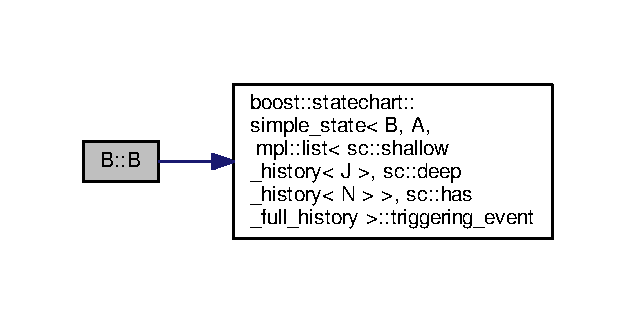
\includegraphics[width=305pt]{struct_b_a8d6359453d0d6206098cf1980b6c7495_cgraph}
\end{center}
\end{figure}
\mbox{\Hypertarget{struct_b_abf3bb815dcba0116aee6f0e87d694702}\label{struct_b_abf3bb815dcba0116aee6f0e87d694702}} 
\index{B@{B}!````~B@{$\sim$B}}
\index{````~B@{$\sim$B}!B@{B}}
\subsubsection{\texorpdfstring{$\sim$\+B()}{~B()}}
{\footnotesize\ttfamily B\+::$\sim$B (\begin{DoxyParamCaption}{ }\end{DoxyParamCaption})\hspace{0.3cm}{\ttfamily [inline]}}

Here is the call graph for this function\+:
\nopagebreak
\begin{figure}[H]
\begin{center}
\leavevmode
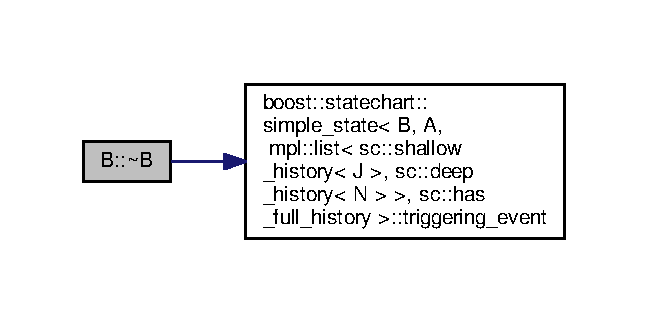
\includegraphics[width=311pt]{struct_b_abf3bb815dcba0116aee6f0e87d694702_cgraph}
\end{center}
\end{figure}


\subsection{Member Function Documentation}
\mbox{\Hypertarget{struct_b_ad8417b0b86326962007c13d75094330e}\label{struct_b_ad8417b0b86326962007c13d75094330e}} 
\index{B@{B}!Do\+It@{Do\+It}}
\index{Do\+It@{Do\+It}!B@{B}}
\subsubsection{\texorpdfstring{Do\+It()}{DoIt()}}
{\footnotesize\ttfamily void B\+::\+Do\+It (\begin{DoxyParamCaption}\item[{const \mbox{\hyperlink{struct_ev_do_it}{Ev\+Do\+It}} \&}]{ }\end{DoxyParamCaption})\hspace{0.3cm}{\ttfamily [inline]}}

Here is the call graph for this function\+:
\nopagebreak
\begin{figure}[H]
\begin{center}
\leavevmode
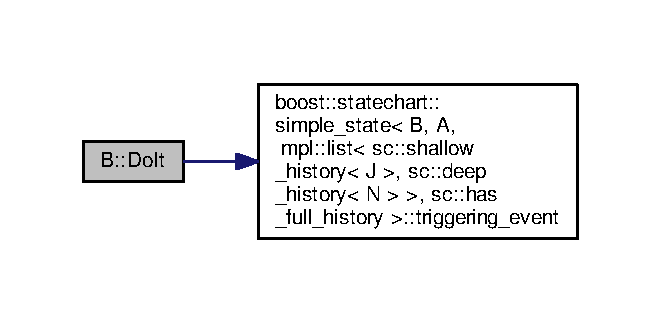
\includegraphics[width=317pt]{struct_b_ad8417b0b86326962007c13d75094330e_cgraph}
\end{center}
\end{figure}
\mbox{\Hypertarget{struct_b_a8eb80df2fcfde5209e4800f5aec2d7a5}\label{struct_b_a8eb80df2fcfde5209e4800f5aec2d7a5}} 
\index{B@{B}!Handle\+Exception@{Handle\+Exception}}
\index{Handle\+Exception@{Handle\+Exception}!B@{B}}
\subsubsection{\texorpdfstring{Handle\+Exception()}{HandleException()}}
{\footnotesize\ttfamily void B\+::\+Handle\+Exception (\begin{DoxyParamCaption}\item[{const \mbox{\hyperlink{classboost_1_1statechart_1_1exception__thrown}{sc\+::exception\+\_\+thrown}} \&}]{ }\end{DoxyParamCaption})\hspace{0.3cm}{\ttfamily [inline]}}

Here is the call graph for this function\+:
\nopagebreak
\begin{figure}[H]
\begin{center}
\leavevmode
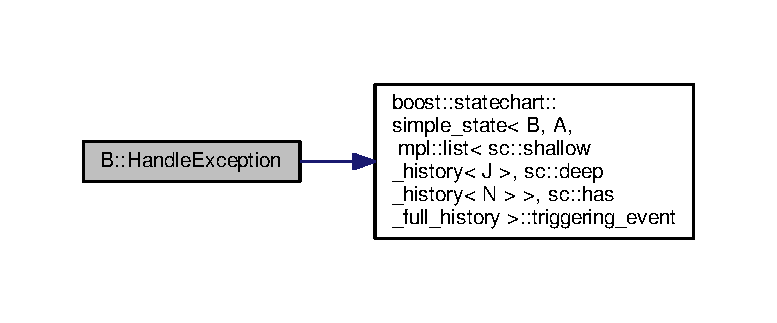
\includegraphics[width=350pt]{struct_b_a8eb80df2fcfde5209e4800f5aec2d7a5_cgraph}
\end{center}
\end{figure}
\mbox{\Hypertarget{struct_b_a862e39288b607fcc7e71f9fa07c0cd20}\label{struct_b_a862e39288b607fcc7e71f9fa07c0cd20}} 
\index{B@{B}!Increment\+Count@{Increment\+Count}}
\index{Increment\+Count@{Increment\+Count}!B@{B}}
\subsubsection{\texorpdfstring{Increment\+Count()}{IncrementCount()}}
{\footnotesize\ttfamily void B\+::\+Increment\+Count (\begin{DoxyParamCaption}\item[{const \mbox{\hyperlink{struct_f}{F}} \&}]{ }\end{DoxyParamCaption})\hspace{0.3cm}{\ttfamily [inline]}}

\mbox{\Hypertarget{struct_b_add69d6626a14cef8f58929dfbe940cb9}\label{struct_b_add69d6626a14cef8f58929dfbe940cb9}} 
\index{B@{B}!react@{react}}
\index{react@{react}!B@{B}}
\subsubsection{\texorpdfstring{react()}{react()}\hspace{0.1cm}{\footnotesize\ttfamily [1/3]}}
{\footnotesize\ttfamily \mbox{\hyperlink{namespaceboost_1_1statechart_abe807f6598b614d6d87bb951ecd92331}{sc\+::result}} B\+::react (\begin{DoxyParamCaption}\item[{const \mbox{\hyperlink{struct_ev_discard_never}{Ev\+Discard\+Never}} \&}]{ }\end{DoxyParamCaption})\hspace{0.3cm}{\ttfamily [inline]}}

Here is the call graph for this function\+:
\nopagebreak
\begin{figure}[H]
\begin{center}
\leavevmode
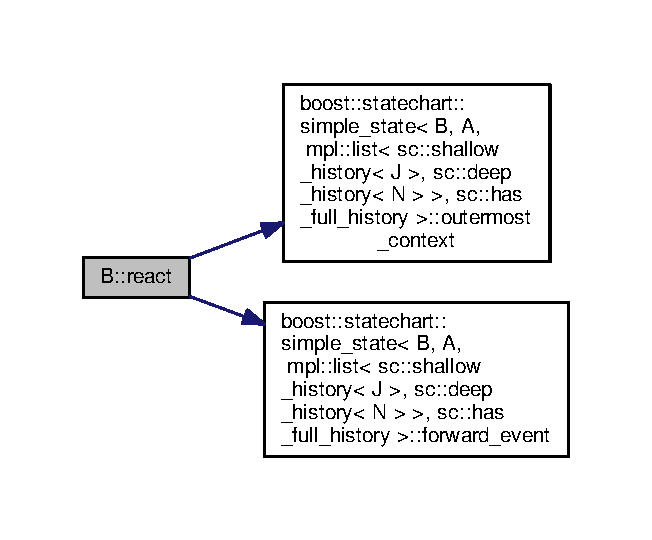
\includegraphics[width=313pt]{struct_b_add69d6626a14cef8f58929dfbe940cb9_cgraph}
\end{center}
\end{figure}
\mbox{\Hypertarget{struct_b_af883c81d64b442ed4252a406a2710459}\label{struct_b_af883c81d64b442ed4252a406a2710459}} 
\index{B@{B}!react@{react}}
\index{react@{react}!B@{B}}
\subsubsection{\texorpdfstring{react()}{react()}\hspace{0.1cm}{\footnotesize\ttfamily [2/3]}}
{\footnotesize\ttfamily \mbox{\hyperlink{namespaceboost_1_1statechart_abe807f6598b614d6d87bb951ecd92331}{sc\+::result}} B\+::react (\begin{DoxyParamCaption}\item[{const \mbox{\hyperlink{struct_ev_discard_in_b}{Ev\+Discard\+InB}} \&}]{ }\end{DoxyParamCaption})\hspace{0.3cm}{\ttfamily [inline]}}

Here is the call graph for this function\+:
\nopagebreak
\begin{figure}[H]
\begin{center}
\leavevmode
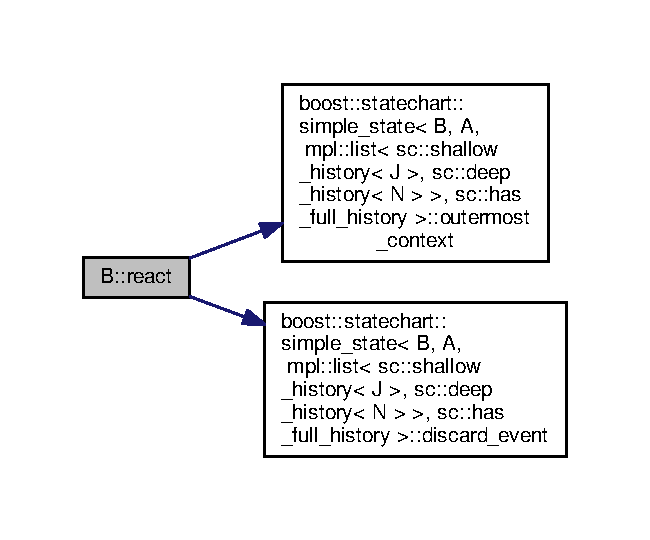
\includegraphics[width=312pt]{struct_b_af883c81d64b442ed4252a406a2710459_cgraph}
\end{center}
\end{figure}
\mbox{\Hypertarget{struct_b_a6ef8f2fd99e04b465b39ea65056ebc10}\label{struct_b_a6ef8f2fd99e04b465b39ea65056ebc10}} 
\index{B@{B}!react@{react}}
\index{react@{react}!B@{B}}
\subsubsection{\texorpdfstring{react()}{react()}\hspace{0.1cm}{\footnotesize\ttfamily [3/3]}}
{\footnotesize\ttfamily \mbox{\hyperlink{namespaceboost_1_1statechart_abe807f6598b614d6d87bb951ecd92331}{sc\+::result}} B\+::react (\begin{DoxyParamCaption}\item[{const \mbox{\hyperlink{struct_ev_discard_in_d}{Ev\+Discard\+InD}} \&}]{ }\end{DoxyParamCaption})\hspace{0.3cm}{\ttfamily [inline]}}

Here is the call graph for this function\+:
\nopagebreak
\begin{figure}[H]
\begin{center}
\leavevmode
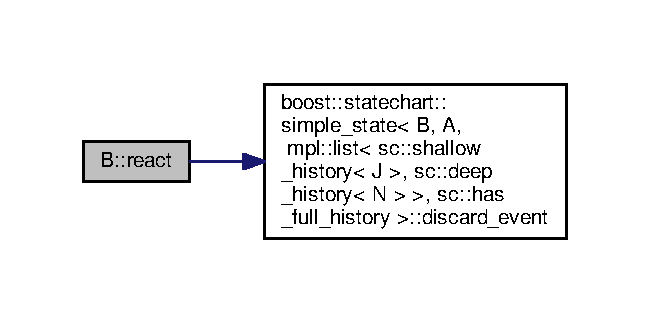
\includegraphics[width=312pt]{struct_b_a6ef8f2fd99e04b465b39ea65056ebc10_cgraph}
\end{center}
\end{figure}


\subsection{Member Data Documentation}
\mbox{\Hypertarget{struct_b_a1a60275928b3599e275f5ba2c34b3a1b}\label{struct_b_a1a60275928b3599e275f5ba2c34b3a1b}} 
\index{B@{B}!event\+Count\+\_\+@{event\+Count\+\_\+}}
\index{event\+Count\+\_\+@{event\+Count\+\_\+}!B@{B}}
\subsubsection{\texorpdfstring{event\+Count\+\_\+}{eventCount\_}}
{\footnotesize\ttfamily unsigned int B\+::event\+Count\+\_\+}



The documentation for this struct was generated from the following files\+:\begin{DoxyCompactItemize}
\item 
test/\mbox{\hyperlink{_custom_reaction_test_8cpp}{Custom\+Reaction\+Test.\+cpp}}\item 
test/\mbox{\hyperlink{_in_state_reaction_test_8cpp}{In\+State\+Reaction\+Test.\+cpp}}\item 
test/\mbox{\hyperlink{_state_cast_test_8cpp}{State\+Cast\+Test.\+cpp}}\item 
test/\mbox{\hyperlink{_state_iteration_test_8cpp}{State\+Iteration\+Test.\+cpp}}\item 
test/\mbox{\hyperlink{_termination_test_8cpp}{Termination\+Test.\+cpp}}\item 
test/\mbox{\hyperlink{_triggering_event_test_8cpp}{Triggering\+Event\+Test.\+cpp}}\end{DoxyCompactItemize}

\hypertarget{struct_ball_returned}{}\section{Ball\+Returned Struct Reference}
\label{struct_ball_returned}\index{Ball\+Returned@{Ball\+Returned}}


{\ttfamily \#include $<$Player.\+hpp$>$}



Inheritance diagram for Ball\+Returned\+:
\nopagebreak
\begin{figure}[H]
\begin{center}
\leavevmode
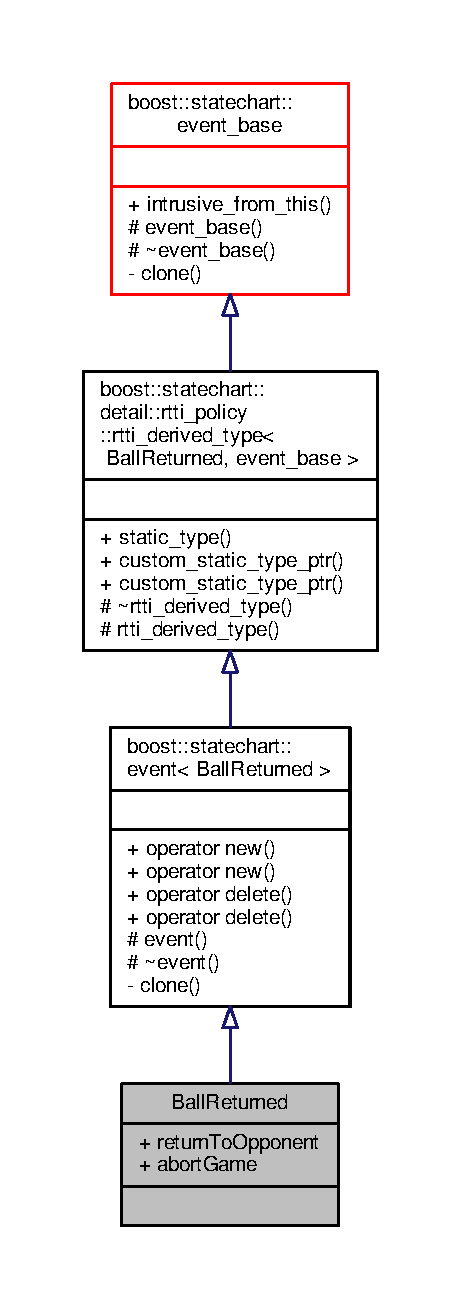
\includegraphics[height=550pt]{struct_ball_returned__inherit__graph}
\end{center}
\end{figure}


Collaboration diagram for Ball\+Returned\+:
\nopagebreak
\begin{figure}[H]
\begin{center}
\leavevmode
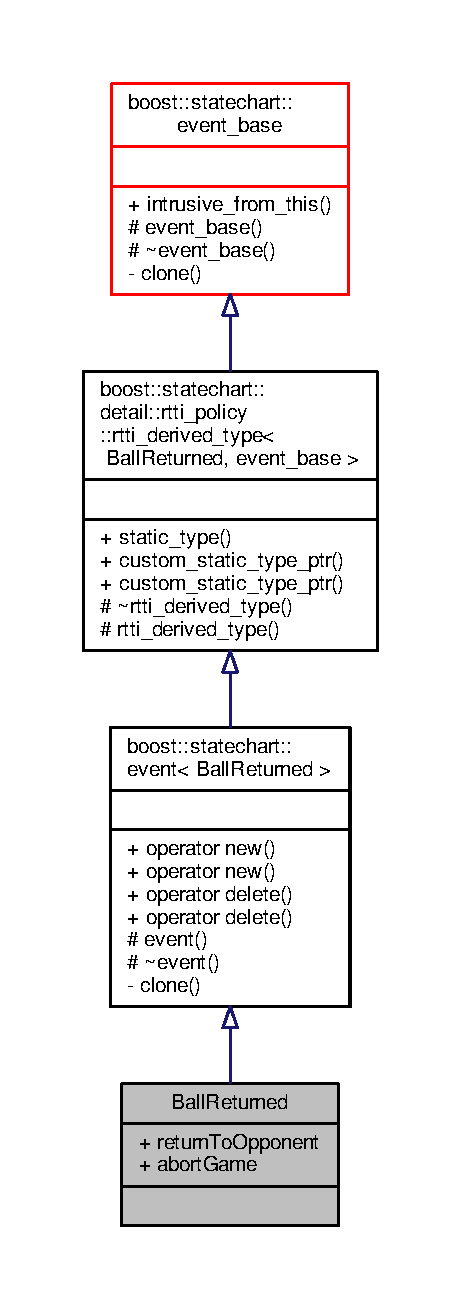
\includegraphics[height=550pt]{struct_ball_returned__coll__graph}
\end{center}
\end{figure}
\subsection*{Public Attributes}
\begin{DoxyCompactItemize}
\item 
boost\+::function1$<$ void, const boost\+::intrusive\+\_\+ptr$<$ const \mbox{\hyperlink{struct_ball_returned}{Ball\+Returned}} $>$ \&$>$ \mbox{\hyperlink{struct_ball_returned_abaa8b43565818174bd1e41234a52bcec}{return\+To\+Opponent}}
\item 
boost\+::function0$<$ void $>$ \mbox{\hyperlink{struct_ball_returned_a8e02be3939205f10a893cac74713deec}{abort\+Game}}
\end{DoxyCompactItemize}
\subsection*{Additional Inherited Members}


\subsection{Member Data Documentation}
\mbox{\Hypertarget{struct_ball_returned_a8e02be3939205f10a893cac74713deec}\label{struct_ball_returned_a8e02be3939205f10a893cac74713deec}} 
\index{Ball\+Returned@{Ball\+Returned}!abort\+Game@{abort\+Game}}
\index{abort\+Game@{abort\+Game}!Ball\+Returned@{Ball\+Returned}}
\subsubsection{\texorpdfstring{abort\+Game}{abortGame}}
{\footnotesize\ttfamily boost\+::function0$<$ void $>$ Ball\+Returned\+::abort\+Game}

\mbox{\Hypertarget{struct_ball_returned_abaa8b43565818174bd1e41234a52bcec}\label{struct_ball_returned_abaa8b43565818174bd1e41234a52bcec}} 
\index{Ball\+Returned@{Ball\+Returned}!return\+To\+Opponent@{return\+To\+Opponent}}
\index{return\+To\+Opponent@{return\+To\+Opponent}!Ball\+Returned@{Ball\+Returned}}
\subsubsection{\texorpdfstring{return\+To\+Opponent}{returnToOpponent}}
{\footnotesize\ttfamily boost\+::function1$<$ void, const boost\+::intrusive\+\_\+ptr$<$ const \mbox{\hyperlink{struct_ball_returned}{Ball\+Returned}} $>$ \& $>$ Ball\+Returned\+::return\+To\+Opponent}



The documentation for this struct was generated from the following file\+:\begin{DoxyCompactItemize}
\item 
example/\+Ping\+Pong/\mbox{\hyperlink{_player_8hpp}{Player.\+hpp}}\end{DoxyCompactItemize}

\hypertarget{structboost_1_1statechart_1_1detail_1_1reaction__dispatcher_1_1base}{}\section{boost\+:\+:statechart\+:\+:detail\+:\+:reaction\+\_\+dispatcher$<$ Reactions, State, Event\+Base, Event, Action\+Context, Id\+Type $>$\+:\+:base Struct Reference}
\label{structboost_1_1statechart_1_1detail_1_1reaction__dispatcher_1_1base}\index{boost\+::statechart\+::detail\+::reaction\+\_\+dispatcher$<$ Reactions, State, Event\+Base, Event, Action\+Context, Id\+Type $>$\+::base@{boost\+::statechart\+::detail\+::reaction\+\_\+dispatcher$<$ Reactions, State, Event\+Base, Event, Action\+Context, Id\+Type $>$\+::base}}


Collaboration diagram for boost\+:\+:statechart\+:\+:detail\+:\+:reaction\+\_\+dispatcher$<$ Reactions, State, Event\+Base, Event, Action\+Context, Id\+Type $>$\+:\+:base\+:
\nopagebreak
\begin{figure}[H]
\begin{center}
\leavevmode
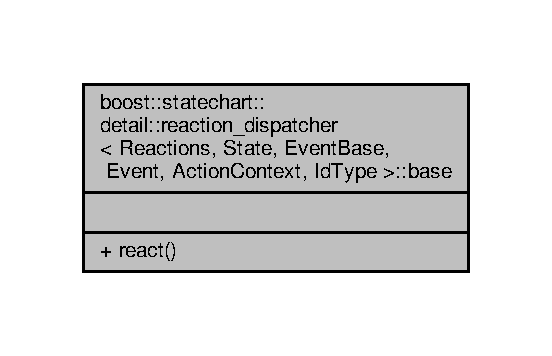
\includegraphics[width=265pt]{structboost_1_1statechart_1_1detail_1_1reaction__dispatcher_1_1base__coll__graph}
\end{center}
\end{figure}
\subsection*{Static Public Member Functions}
\begin{DoxyCompactItemize}
\item 
static \mbox{\hyperlink{namespaceboost_1_1statechart_abe807f6598b614d6d87bb951ecd92331}{result}} \mbox{\hyperlink{structboost_1_1statechart_1_1detail_1_1reaction__dispatcher_1_1base_acc2a12ce404e84665adf2b53ad6be6c0}{react}} (State \&stt, const Event\+Base \&evt, const Id\+Type \&)
\end{DoxyCompactItemize}


\subsection{Member Function Documentation}
\mbox{\Hypertarget{structboost_1_1statechart_1_1detail_1_1reaction__dispatcher_1_1base_acc2a12ce404e84665adf2b53ad6be6c0}\label{structboost_1_1statechart_1_1detail_1_1reaction__dispatcher_1_1base_acc2a12ce404e84665adf2b53ad6be6c0}} 
\index{boost\+::statechart\+::detail\+::reaction\+\_\+dispatcher\+::base@{boost\+::statechart\+::detail\+::reaction\+\_\+dispatcher\+::base}!react@{react}}
\index{react@{react}!boost\+::statechart\+::detail\+::reaction\+\_\+dispatcher\+::base@{boost\+::statechart\+::detail\+::reaction\+\_\+dispatcher\+::base}}
\subsubsection{\texorpdfstring{react()}{react()}}
{\footnotesize\ttfamily template$<$class Reactions , class State , class Event\+Base , class Event , class Action\+Context , class Id\+Type $>$ \\
static \mbox{\hyperlink{namespaceboost_1_1statechart_abe807f6598b614d6d87bb951ecd92331}{result}} \mbox{\hyperlink{classboost_1_1statechart_1_1detail_1_1reaction__dispatcher}{boost\+::statechart\+::detail\+::reaction\+\_\+dispatcher}}$<$ Reactions, State, Event\+Base, Event, Action\+Context, Id\+Type $>$\+::base\+::react (\begin{DoxyParamCaption}\item[{State \&}]{stt,  }\item[{const Event\+Base \&}]{evt,  }\item[{const Id\+Type \&}]{ }\end{DoxyParamCaption})\hspace{0.3cm}{\ttfamily [inline]}, {\ttfamily [static]}}



The documentation for this struct was generated from the following file\+:\begin{DoxyCompactItemize}
\item 
include/boost/statechart/detail/\mbox{\hyperlink{reaction__dispatcher_8hpp}{reaction\+\_\+dispatcher.\+hpp}}\end{DoxyCompactItemize}

\hypertarget{structboost_1_1statechart_1_1detail_1_1reaction__dispatcher_1_1base__with__action}{}\section{boost\+:\+:statechart\+:\+:detail\+:\+:reaction\+\_\+dispatcher$<$ Reactions, State, Event\+Base, Event, Action\+Context, Id\+Type $>$\+:\+:base\+\_\+with\+\_\+action Struct Reference}
\label{structboost_1_1statechart_1_1detail_1_1reaction__dispatcher_1_1base__with__action}\index{boost\+::statechart\+::detail\+::reaction\+\_\+dispatcher$<$ Reactions, State, Event\+Base, Event, Action\+Context, Id\+Type $>$\+::base\+\_\+with\+\_\+action@{boost\+::statechart\+::detail\+::reaction\+\_\+dispatcher$<$ Reactions, State, Event\+Base, Event, Action\+Context, Id\+Type $>$\+::base\+\_\+with\+\_\+action}}


Collaboration diagram for boost\+:\+:statechart\+:\+:detail\+:\+:reaction\+\_\+dispatcher$<$ Reactions, State, Event\+Base, Event, Action\+Context, Id\+Type $>$\+:\+:base\+\_\+with\+\_\+action\+:
\nopagebreak
\begin{figure}[H]
\begin{center}
\leavevmode
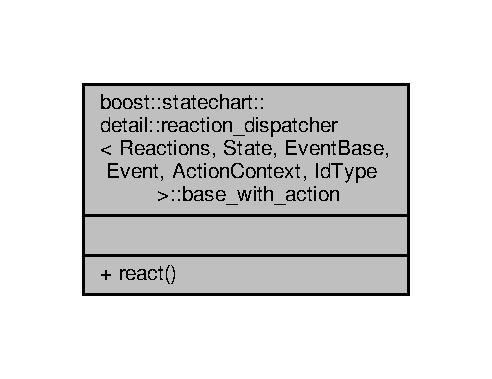
\includegraphics[width=236pt]{structboost_1_1statechart_1_1detail_1_1reaction__dispatcher_1_1base__with__action__coll__graph}
\end{center}
\end{figure}
\subsection*{Static Public Member Functions}
\begin{DoxyCompactItemize}
\item 
static \mbox{\hyperlink{namespaceboost_1_1statechart_abe807f6598b614d6d87bb951ecd92331}{result}} \mbox{\hyperlink{structboost_1_1statechart_1_1detail_1_1reaction__dispatcher_1_1base__with__action_a325fa0584944412ec6e24377c1b67dfc}{react}} (State \&stt, const Event\+Base \&evt)
\end{DoxyCompactItemize}


\subsection{Member Function Documentation}
\mbox{\Hypertarget{structboost_1_1statechart_1_1detail_1_1reaction__dispatcher_1_1base__with__action_a325fa0584944412ec6e24377c1b67dfc}\label{structboost_1_1statechart_1_1detail_1_1reaction__dispatcher_1_1base__with__action_a325fa0584944412ec6e24377c1b67dfc}} 
\index{boost\+::statechart\+::detail\+::reaction\+\_\+dispatcher\+::base\+\_\+with\+\_\+action@{boost\+::statechart\+::detail\+::reaction\+\_\+dispatcher\+::base\+\_\+with\+\_\+action}!react@{react}}
\index{react@{react}!boost\+::statechart\+::detail\+::reaction\+\_\+dispatcher\+::base\+\_\+with\+\_\+action@{boost\+::statechart\+::detail\+::reaction\+\_\+dispatcher\+::base\+\_\+with\+\_\+action}}
\subsubsection{\texorpdfstring{react()}{react()}}
{\footnotesize\ttfamily template$<$class Reactions , class State , class Event\+Base , class Event , class Action\+Context , class Id\+Type $>$ \\
static \mbox{\hyperlink{namespaceboost_1_1statechart_abe807f6598b614d6d87bb951ecd92331}{result}} \mbox{\hyperlink{classboost_1_1statechart_1_1detail_1_1reaction__dispatcher}{boost\+::statechart\+::detail\+::reaction\+\_\+dispatcher}}$<$ Reactions, State, Event\+Base, Event, Action\+Context, Id\+Type $>$\+::base\+\_\+with\+\_\+action\+::react (\begin{DoxyParamCaption}\item[{State \&}]{stt,  }\item[{const Event\+Base \&}]{evt }\end{DoxyParamCaption})\hspace{0.3cm}{\ttfamily [inline]}, {\ttfamily [static]}}



The documentation for this struct was generated from the following file\+:\begin{DoxyCompactItemize}
\item 
include/boost/statechart/detail/\mbox{\hyperlink{reaction__dispatcher_8hpp}{reaction\+\_\+dispatcher.\+hpp}}\end{DoxyCompactItemize}

\hypertarget{struct_bit_machine}{}\section{Bit\+Machine$<$ No\+Of\+Bits, First\+Transition\+Bit $>$ Struct Template Reference}
\label{struct_bit_machine}\index{Bit\+Machine$<$ No\+Of\+Bits, First\+Transition\+Bit $>$@{Bit\+Machine$<$ No\+Of\+Bits, First\+Transition\+Bit $>$}}


Inheritance diagram for Bit\+Machine$<$ No\+Of\+Bits, First\+Transition\+Bit $>$\+:
\nopagebreak
\begin{figure}[H]
\begin{center}
\leavevmode
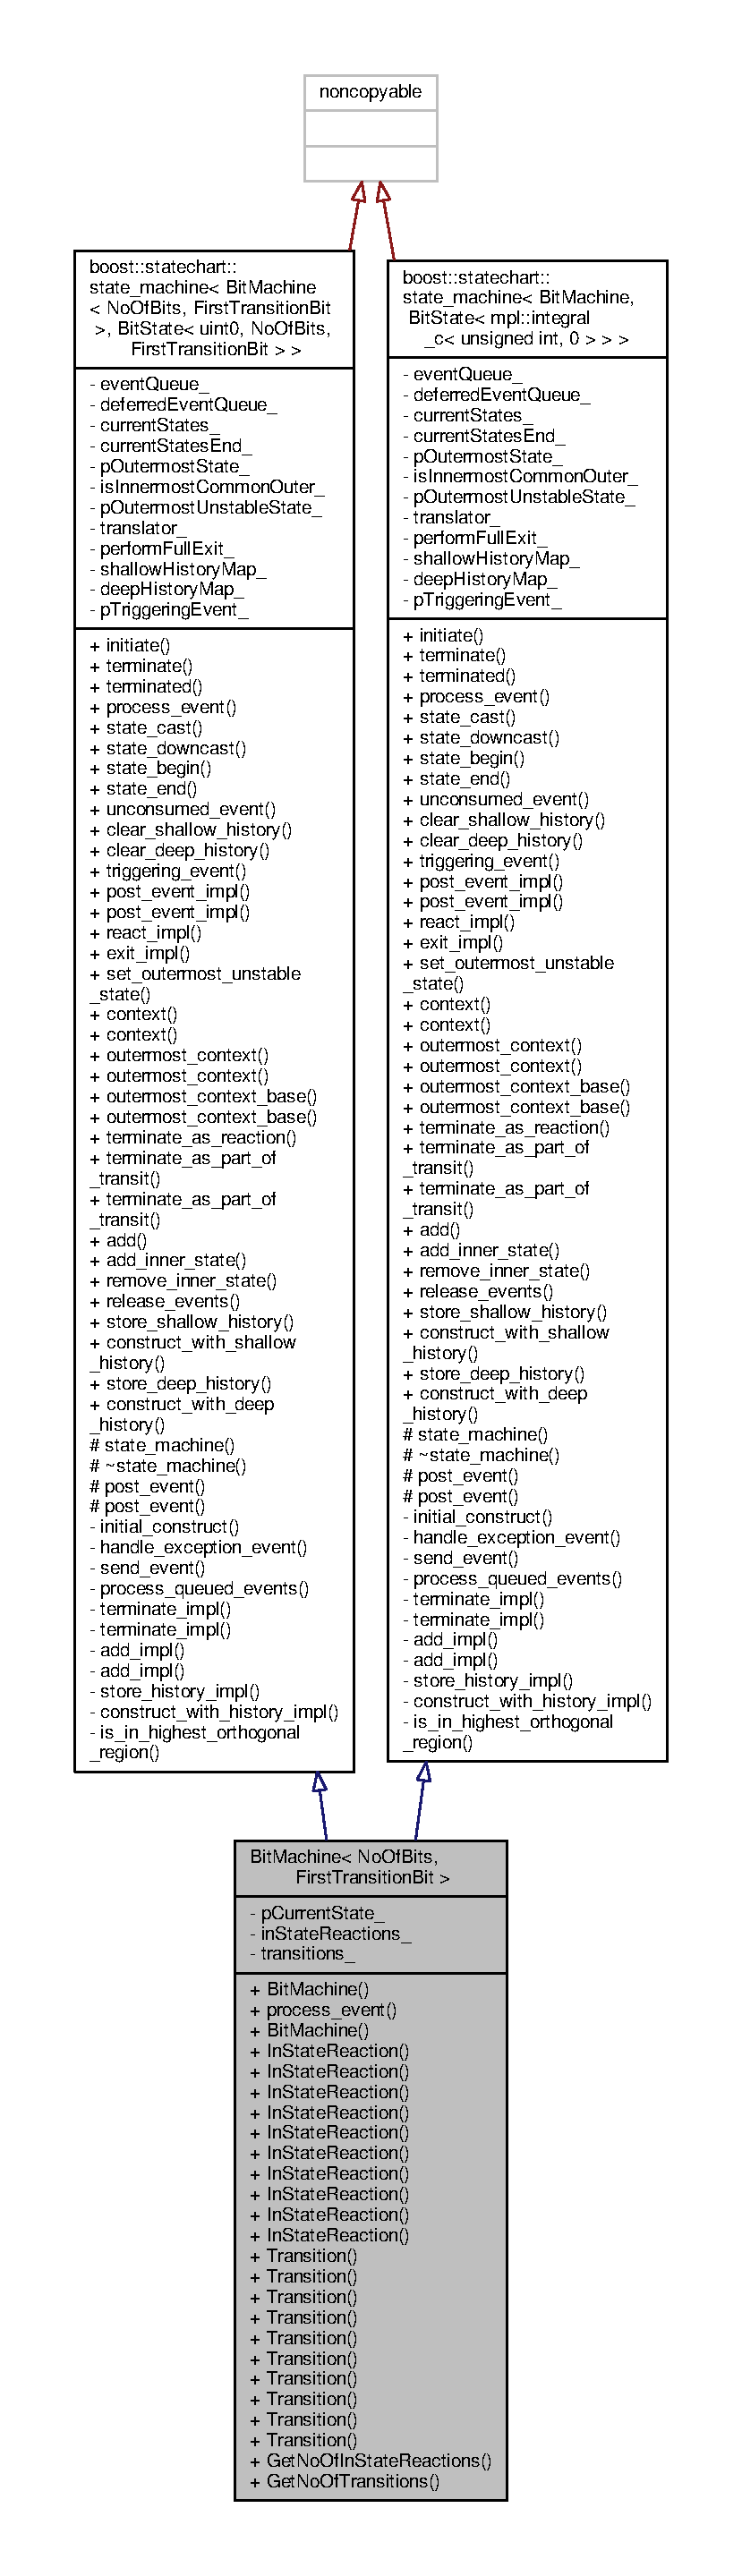
\includegraphics[height=550pt]{struct_bit_machine__inherit__graph}
\end{center}
\end{figure}


Collaboration diagram for Bit\+Machine$<$ No\+Of\+Bits, First\+Transition\+Bit $>$\+:
\nopagebreak
\begin{figure}[H]
\begin{center}
\leavevmode
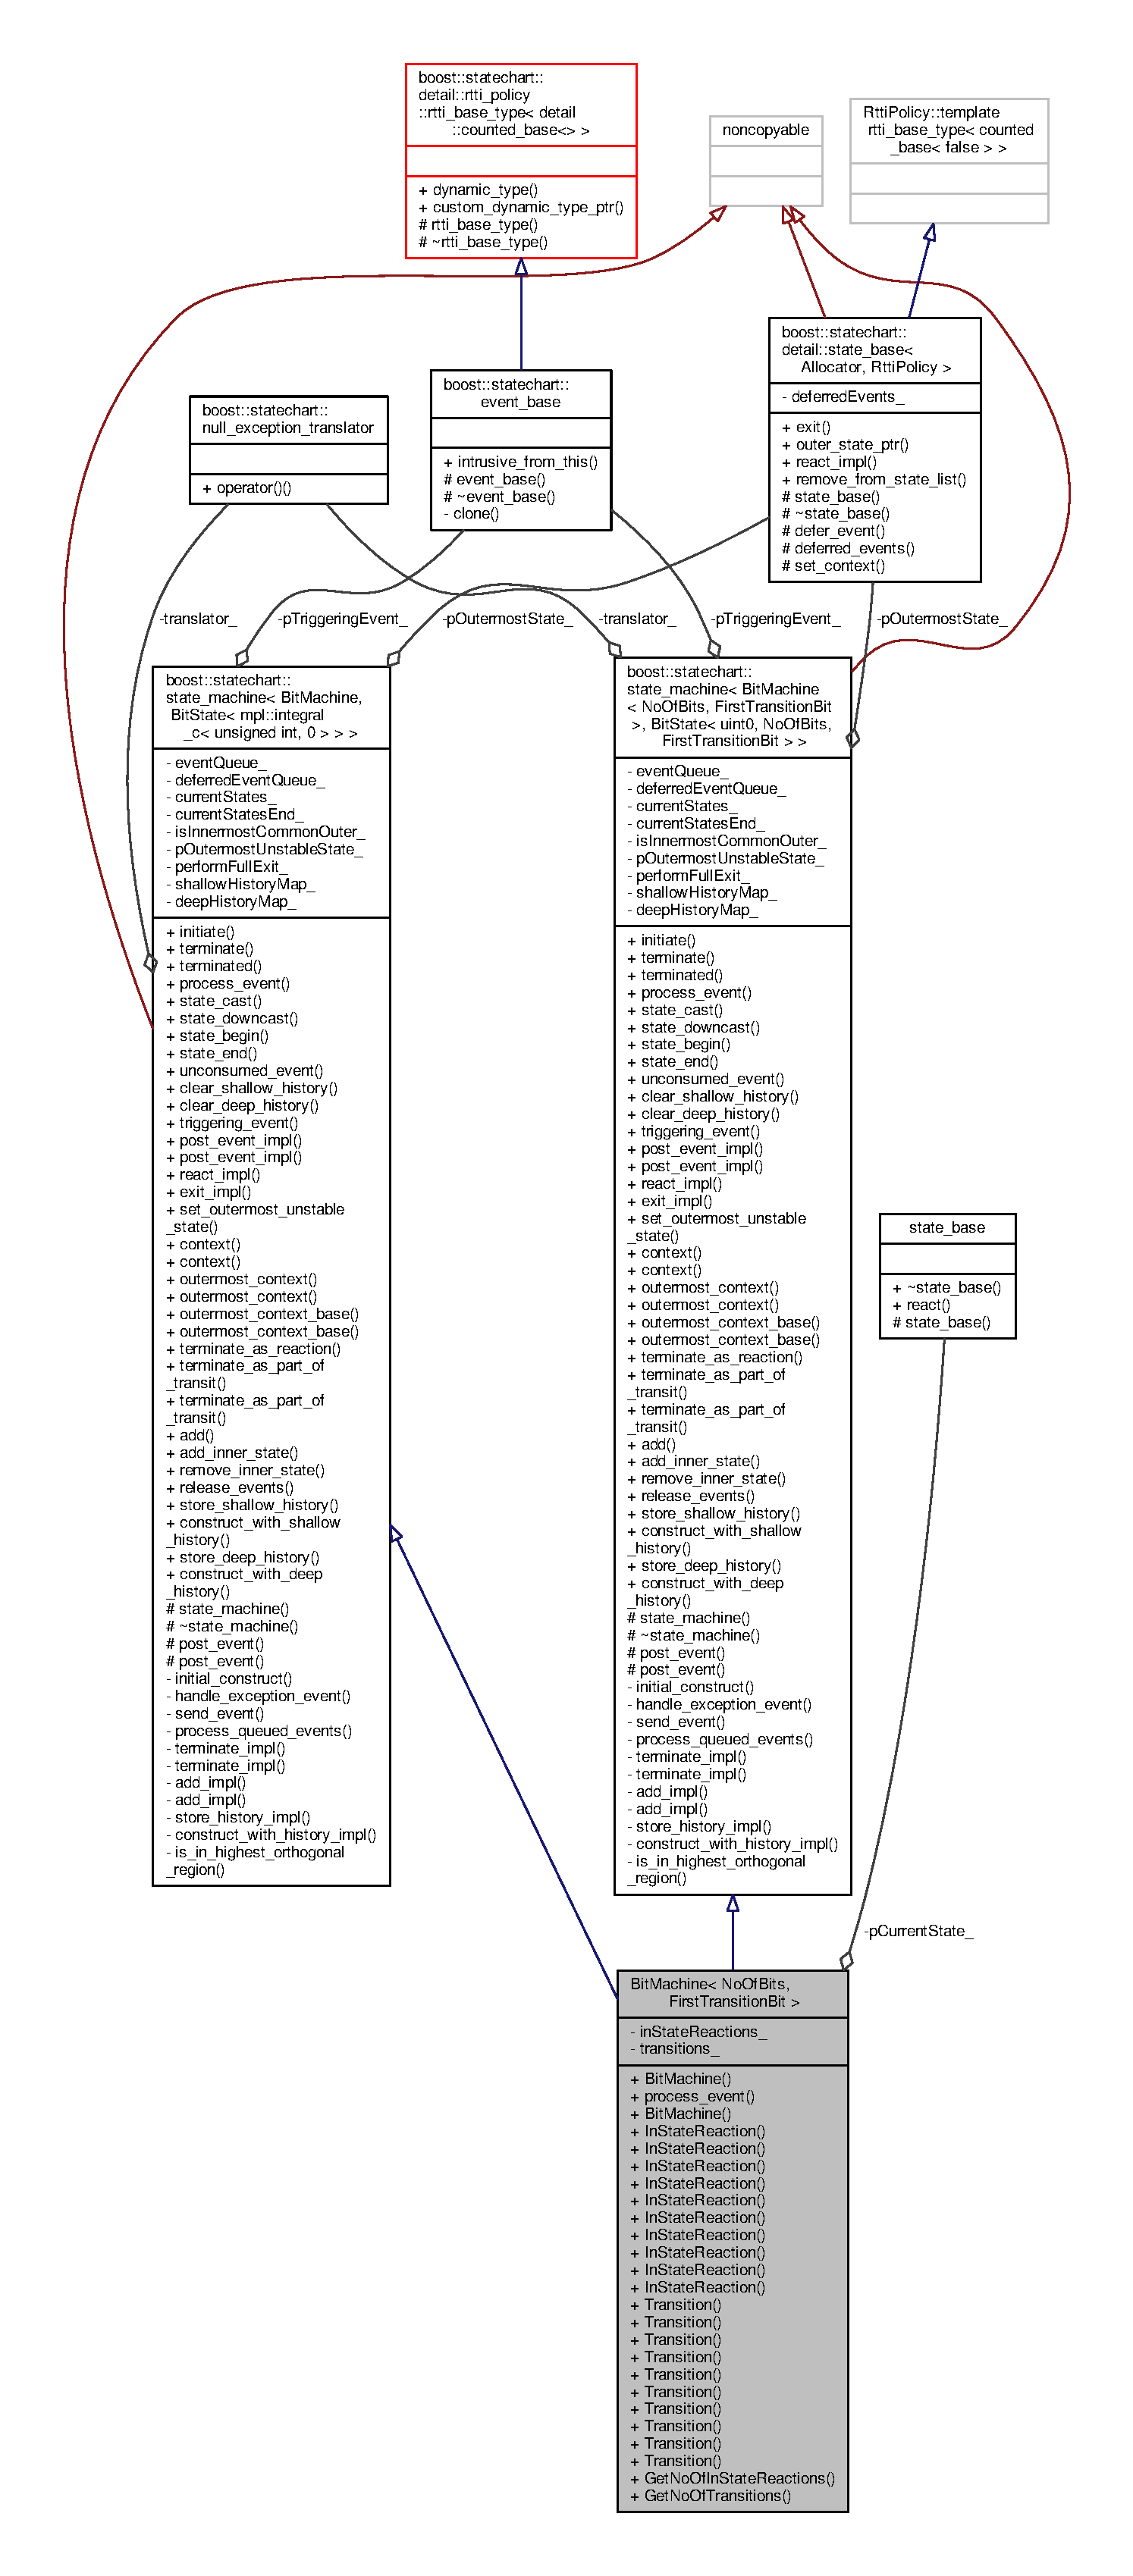
\includegraphics[height=550pt]{struct_bit_machine__coll__graph}
\end{center}
\end{figure}
\subsection*{Classes}
\begin{DoxyCompactItemize}
\item 
struct \mbox{\hyperlink{struct_bit_machine_1_1_off}{Off}}
\item 
struct \mbox{\hyperlink{struct_bit_machine_1_1_on}{On}}
\end{DoxyCompactItemize}
\subsection*{Public Member Functions}
\begin{DoxyCompactItemize}
\item 
\mbox{\hyperlink{struct_bit_machine_a58f14b49b03c4763e3c4b8737ba285fe}{Bit\+Machine}} ()
\item 
void \mbox{\hyperlink{struct_bit_machine_ae77e5375e470002e98bde6307793b102}{process\+\_\+event}} (const \mbox{\hyperlink{classevent__base}{event\+\_\+base}} \&evt)
\item 
\mbox{\hyperlink{struct_bit_machine_a58f14b49b03c4763e3c4b8737ba285fe}{Bit\+Machine}} ()
\item 
void \mbox{\hyperlink{struct_bit_machine_afca2097dd81c0e01f7a7bafc0cb7f97b}{In\+State\+Reaction}} (const \mbox{\hyperlink{struct_ev_flip_bit}{Ev\+Flip\+Bit}}$<$ \mbox{\hyperlink{_performance_8cpp_ac4323a4a68daf3126a7be25628f1d622}{uint0}} $>$ \&)
\item 
void \mbox{\hyperlink{struct_bit_machine_a3e3d1636ee5cdee7fbf9bc4311dad61d}{In\+State\+Reaction}} (const \mbox{\hyperlink{struct_ev_flip_bit}{Ev\+Flip\+Bit}}$<$ \mbox{\hyperlink{_performance_8cpp_afada4030cdd8c9628ca412e4409d07d1}{uint1}} $>$ \&)
\item 
void \mbox{\hyperlink{struct_bit_machine_a0070c2dc29514f2904c388f531e0a568}{In\+State\+Reaction}} (const \mbox{\hyperlink{struct_ev_flip_bit}{Ev\+Flip\+Bit}}$<$ \mbox{\hyperlink{_performance_8cpp_ad7cf25dde7cbe398d57ed74b7109aaaa}{uint2}} $>$ \&)
\item 
void \mbox{\hyperlink{struct_bit_machine_a91742d27fd72fa6c301116f5618a6489}{In\+State\+Reaction}} (const \mbox{\hyperlink{struct_ev_flip_bit}{Ev\+Flip\+Bit}}$<$ \mbox{\hyperlink{_performance_8cpp_a487e33775f12c3ab023e66546a69810f}{uint3}} $>$ \&)
\item 
void \mbox{\hyperlink{struct_bit_machine_abf277c6f89800d794ca2bbaba62de89b}{In\+State\+Reaction}} (const \mbox{\hyperlink{struct_ev_flip_bit}{Ev\+Flip\+Bit}}$<$ \mbox{\hyperlink{_performance_8cpp_aa143aaac7fcfe524f6f4f33cc878ae95}{uint4}} $>$ \&)
\item 
void \mbox{\hyperlink{struct_bit_machine_a9b51c97e12366b4895b1b161e06c826f}{In\+State\+Reaction}} (const \mbox{\hyperlink{struct_ev_flip_bit}{Ev\+Flip\+Bit}}$<$ \mbox{\hyperlink{_performance_8cpp_a34732dbaa46d46251e4ac1faef9fcecd}{uint5}} $>$ \&)
\item 
void \mbox{\hyperlink{struct_bit_machine_aa3060810568983a875d87205613e2b68}{In\+State\+Reaction}} (const \mbox{\hyperlink{struct_ev_flip_bit}{Ev\+Flip\+Bit}}$<$ \mbox{\hyperlink{_performance_8cpp_a76e4a9cf398589b4ad27852c9f4389f9}{uint6}} $>$ \&)
\item 
void \mbox{\hyperlink{struct_bit_machine_a141e630cf0be7c330a5ef019cbdb5cf5}{In\+State\+Reaction}} (const \mbox{\hyperlink{struct_ev_flip_bit}{Ev\+Flip\+Bit}}$<$ \mbox{\hyperlink{_performance_8cpp_ae332b751ff9ebef63d125fdaaaf45f8c}{uint7}} $>$ \&)
\item 
void \mbox{\hyperlink{struct_bit_machine_a3a793d4f5cda90bcd4fee1acf553a1b1}{In\+State\+Reaction}} (const \mbox{\hyperlink{struct_ev_flip_bit}{Ev\+Flip\+Bit}}$<$ \mbox{\hyperlink{_performance_8cpp_acf7191ac01fae99fae3f5a89e4f8a8ff}{uint8}} $>$ \&)
\item 
void \mbox{\hyperlink{struct_bit_machine_af8868edd3c7e77b3630278c1fd47247c}{In\+State\+Reaction}} (const \mbox{\hyperlink{struct_ev_flip_bit}{Ev\+Flip\+Bit}}$<$ \mbox{\hyperlink{_performance_8cpp_ac1d5f5aee5a76e77d960741a1bd84b12}{uint9}} $>$ \&)
\item 
void \mbox{\hyperlink{struct_bit_machine_a43a10ef23aab14065277c1bc34d08007}{Transition}} (const \mbox{\hyperlink{struct_ev_flip_bit}{Ev\+Flip\+Bit}}$<$ \mbox{\hyperlink{_performance_8cpp_ac4323a4a68daf3126a7be25628f1d622}{uint0}} $>$ \&)
\item 
void \mbox{\hyperlink{struct_bit_machine_a75b74e2bcb9417cad75dabe92e4663fc}{Transition}} (const \mbox{\hyperlink{struct_ev_flip_bit}{Ev\+Flip\+Bit}}$<$ \mbox{\hyperlink{_performance_8cpp_afada4030cdd8c9628ca412e4409d07d1}{uint1}} $>$ \&)
\item 
void \mbox{\hyperlink{struct_bit_machine_a0eef1a8ac436d26db1920032bc81186b}{Transition}} (const \mbox{\hyperlink{struct_ev_flip_bit}{Ev\+Flip\+Bit}}$<$ \mbox{\hyperlink{_performance_8cpp_ad7cf25dde7cbe398d57ed74b7109aaaa}{uint2}} $>$ \&)
\item 
void \mbox{\hyperlink{struct_bit_machine_a065addd94fcc6c7046e700da2d170370}{Transition}} (const \mbox{\hyperlink{struct_ev_flip_bit}{Ev\+Flip\+Bit}}$<$ \mbox{\hyperlink{_performance_8cpp_a487e33775f12c3ab023e66546a69810f}{uint3}} $>$ \&)
\item 
void \mbox{\hyperlink{struct_bit_machine_a7a095e344792b70a069ee44fbd6f2e3a}{Transition}} (const \mbox{\hyperlink{struct_ev_flip_bit}{Ev\+Flip\+Bit}}$<$ \mbox{\hyperlink{_performance_8cpp_aa143aaac7fcfe524f6f4f33cc878ae95}{uint4}} $>$ \&)
\item 
void \mbox{\hyperlink{struct_bit_machine_a6ae4632116970d2f52185f71e086c37d}{Transition}} (const \mbox{\hyperlink{struct_ev_flip_bit}{Ev\+Flip\+Bit}}$<$ \mbox{\hyperlink{_performance_8cpp_a34732dbaa46d46251e4ac1faef9fcecd}{uint5}} $>$ \&)
\item 
void \mbox{\hyperlink{struct_bit_machine_aa139bb8076c9041eae686111879dbdd1}{Transition}} (const \mbox{\hyperlink{struct_ev_flip_bit}{Ev\+Flip\+Bit}}$<$ \mbox{\hyperlink{_performance_8cpp_a76e4a9cf398589b4ad27852c9f4389f9}{uint6}} $>$ \&)
\item 
void \mbox{\hyperlink{struct_bit_machine_a006a8fcc19034fae402a95505f3ccafe}{Transition}} (const \mbox{\hyperlink{struct_ev_flip_bit}{Ev\+Flip\+Bit}}$<$ \mbox{\hyperlink{_performance_8cpp_ae332b751ff9ebef63d125fdaaaf45f8c}{uint7}} $>$ \&)
\item 
void \mbox{\hyperlink{struct_bit_machine_a1ee9e973bde376f8b952b6ad14b6b246}{Transition}} (const \mbox{\hyperlink{struct_ev_flip_bit}{Ev\+Flip\+Bit}}$<$ \mbox{\hyperlink{_performance_8cpp_acf7191ac01fae99fae3f5a89e4f8a8ff}{uint8}} $>$ \&)
\item 
void \mbox{\hyperlink{struct_bit_machine_a3ef5a60f15cd15bb46b63d2a86594c5a}{Transition}} (const \mbox{\hyperlink{struct_ev_flip_bit}{Ev\+Flip\+Bit}}$<$ \mbox{\hyperlink{_performance_8cpp_ac1d5f5aee5a76e77d960741a1bd84b12}{uint9}} $>$ \&)
\item 
unsigned int \mbox{\hyperlink{struct_bit_machine_a7e488a02bcdc1984dd078aff1db33ce1}{Get\+No\+Of\+In\+State\+Reactions}} () const
\item 
unsigned int \mbox{\hyperlink{struct_bit_machine_a1e02c163421c8981a86405ed8c83c9c0}{Get\+No\+Of\+Transitions}} () const
\end{DoxyCompactItemize}
\subsection*{Private Attributes}
\begin{DoxyCompactItemize}
\item 
const \mbox{\hyperlink{classstate__base}{state\+\_\+base}} $\ast$ \mbox{\hyperlink{struct_bit_machine_a22ecd751130c63597ce80ca5c1d9bff3}{p\+Current\+State\+\_\+}}
\item 
unsigned int \mbox{\hyperlink{struct_bit_machine_ad35b2868f25bc77b9b9db1f1e9d03c8b}{in\+State\+Reactions\+\_\+}}
\item 
unsigned int \mbox{\hyperlink{struct_bit_machine_a042875c3dcc1ff444ddd45df5ca47c56}{transitions\+\_\+}}
\end{DoxyCompactItemize}
\subsection*{Additional Inherited Members}


\subsection{Constructor \& Destructor Documentation}
\mbox{\Hypertarget{struct_bit_machine_a58f14b49b03c4763e3c4b8737ba285fe}\label{struct_bit_machine_a58f14b49b03c4763e3c4b8737ba285fe}} 
\index{Bit\+Machine@{Bit\+Machine}!Bit\+Machine@{Bit\+Machine}}
\index{Bit\+Machine@{Bit\+Machine}!Bit\+Machine@{Bit\+Machine}}
\subsubsection{\texorpdfstring{Bit\+Machine()}{BitMachine()}\hspace{0.1cm}{\footnotesize\ttfamily [1/2]}}
{\footnotesize\ttfamily template$<$class No\+Of\+Bits, class First\+Transition\+Bit$>$ \\
\mbox{\hyperlink{struct_bit_machine}{Bit\+Machine}}$<$ No\+Of\+Bits, First\+Transition\+Bit $>$\+::\mbox{\hyperlink{struct_bit_machine}{Bit\+Machine}} (\begin{DoxyParamCaption}{ }\end{DoxyParamCaption})\hspace{0.3cm}{\ttfamily [inline]}}

\mbox{\Hypertarget{struct_bit_machine_a58f14b49b03c4763e3c4b8737ba285fe}\label{struct_bit_machine_a58f14b49b03c4763e3c4b8737ba285fe}} 
\index{Bit\+Machine@{Bit\+Machine}!Bit\+Machine@{Bit\+Machine}}
\index{Bit\+Machine@{Bit\+Machine}!Bit\+Machine@{Bit\+Machine}}
\subsubsection{\texorpdfstring{Bit\+Machine()}{BitMachine()}\hspace{0.1cm}{\footnotesize\ttfamily [2/2]}}
{\footnotesize\ttfamily template$<$class No\+Of\+Bits, class First\+Transition\+Bit$>$ \\
\mbox{\hyperlink{struct_bit_machine}{Bit\+Machine}}$<$ No\+Of\+Bits, First\+Transition\+Bit $>$\+::\mbox{\hyperlink{struct_bit_machine}{Bit\+Machine}} (\begin{DoxyParamCaption}{ }\end{DoxyParamCaption})\hspace{0.3cm}{\ttfamily [inline]}}



\subsection{Member Function Documentation}
\mbox{\Hypertarget{struct_bit_machine_a7e488a02bcdc1984dd078aff1db33ce1}\label{struct_bit_machine_a7e488a02bcdc1984dd078aff1db33ce1}} 
\index{Bit\+Machine@{Bit\+Machine}!Get\+No\+Of\+In\+State\+Reactions@{Get\+No\+Of\+In\+State\+Reactions}}
\index{Get\+No\+Of\+In\+State\+Reactions@{Get\+No\+Of\+In\+State\+Reactions}!Bit\+Machine@{Bit\+Machine}}
\subsubsection{\texorpdfstring{Get\+No\+Of\+In\+State\+Reactions()}{GetNoOfInStateReactions()}}
{\footnotesize\ttfamily template$<$class No\+Of\+Bits, class First\+Transition\+Bit$>$ \\
unsigned int \mbox{\hyperlink{struct_bit_machine}{Bit\+Machine}}$<$ No\+Of\+Bits, First\+Transition\+Bit $>$\+::Get\+No\+Of\+In\+State\+Reactions (\begin{DoxyParamCaption}{ }\end{DoxyParamCaption}) const\hspace{0.3cm}{\ttfamily [inline]}}

Here is the caller graph for this function\+:
\nopagebreak
\begin{figure}[H]
\begin{center}
\leavevmode
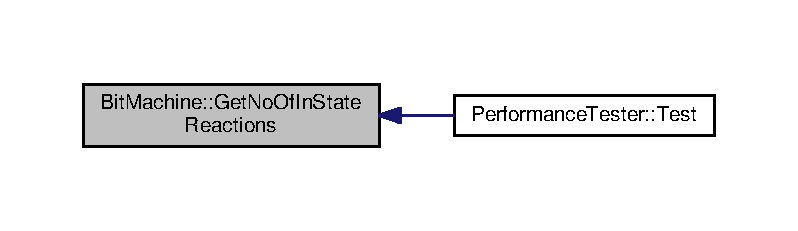
\includegraphics[width=350pt]{struct_bit_machine_a7e488a02bcdc1984dd078aff1db33ce1_icgraph}
\end{center}
\end{figure}
\mbox{\Hypertarget{struct_bit_machine_a1e02c163421c8981a86405ed8c83c9c0}\label{struct_bit_machine_a1e02c163421c8981a86405ed8c83c9c0}} 
\index{Bit\+Machine@{Bit\+Machine}!Get\+No\+Of\+Transitions@{Get\+No\+Of\+Transitions}}
\index{Get\+No\+Of\+Transitions@{Get\+No\+Of\+Transitions}!Bit\+Machine@{Bit\+Machine}}
\subsubsection{\texorpdfstring{Get\+No\+Of\+Transitions()}{GetNoOfTransitions()}}
{\footnotesize\ttfamily template$<$class No\+Of\+Bits, class First\+Transition\+Bit$>$ \\
unsigned int \mbox{\hyperlink{struct_bit_machine}{Bit\+Machine}}$<$ No\+Of\+Bits, First\+Transition\+Bit $>$\+::Get\+No\+Of\+Transitions (\begin{DoxyParamCaption}{ }\end{DoxyParamCaption}) const\hspace{0.3cm}{\ttfamily [inline]}}

Here is the caller graph for this function\+:
\nopagebreak
\begin{figure}[H]
\begin{center}
\leavevmode
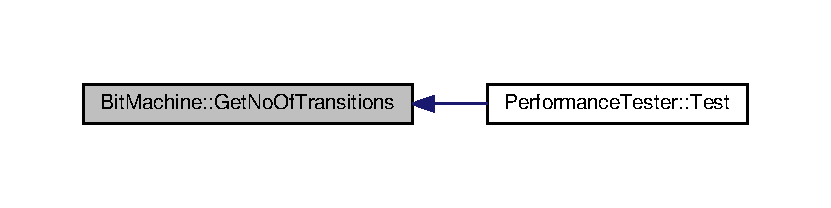
\includegraphics[width=350pt]{struct_bit_machine_a1e02c163421c8981a86405ed8c83c9c0_icgraph}
\end{center}
\end{figure}
\mbox{\Hypertarget{struct_bit_machine_afca2097dd81c0e01f7a7bafc0cb7f97b}\label{struct_bit_machine_afca2097dd81c0e01f7a7bafc0cb7f97b}} 
\index{Bit\+Machine@{Bit\+Machine}!In\+State\+Reaction@{In\+State\+Reaction}}
\index{In\+State\+Reaction@{In\+State\+Reaction}!Bit\+Machine@{Bit\+Machine}}
\subsubsection{\texorpdfstring{In\+State\+Reaction()}{InStateReaction()}\hspace{0.1cm}{\footnotesize\ttfamily [1/10]}}
{\footnotesize\ttfamily template$<$class No\+Of\+Bits, class First\+Transition\+Bit$>$ \\
void \mbox{\hyperlink{struct_bit_machine}{Bit\+Machine}}$<$ No\+Of\+Bits, First\+Transition\+Bit $>$\+::In\+State\+Reaction (\begin{DoxyParamCaption}\item[{const \mbox{\hyperlink{struct_ev_flip_bit}{Ev\+Flip\+Bit}}$<$ \mbox{\hyperlink{_performance_8cpp_ac4323a4a68daf3126a7be25628f1d622}{uint0}} $>$ \&}]{ }\end{DoxyParamCaption})\hspace{0.3cm}{\ttfamily [inline]}}

\mbox{\Hypertarget{struct_bit_machine_a3e3d1636ee5cdee7fbf9bc4311dad61d}\label{struct_bit_machine_a3e3d1636ee5cdee7fbf9bc4311dad61d}} 
\index{Bit\+Machine@{Bit\+Machine}!In\+State\+Reaction@{In\+State\+Reaction}}
\index{In\+State\+Reaction@{In\+State\+Reaction}!Bit\+Machine@{Bit\+Machine}}
\subsubsection{\texorpdfstring{In\+State\+Reaction()}{InStateReaction()}\hspace{0.1cm}{\footnotesize\ttfamily [2/10]}}
{\footnotesize\ttfamily template$<$class No\+Of\+Bits, class First\+Transition\+Bit$>$ \\
void \mbox{\hyperlink{struct_bit_machine}{Bit\+Machine}}$<$ No\+Of\+Bits, First\+Transition\+Bit $>$\+::In\+State\+Reaction (\begin{DoxyParamCaption}\item[{const \mbox{\hyperlink{struct_ev_flip_bit}{Ev\+Flip\+Bit}}$<$ \mbox{\hyperlink{_performance_8cpp_afada4030cdd8c9628ca412e4409d07d1}{uint1}} $>$ \&}]{ }\end{DoxyParamCaption})\hspace{0.3cm}{\ttfamily [inline]}}

\mbox{\Hypertarget{struct_bit_machine_a0070c2dc29514f2904c388f531e0a568}\label{struct_bit_machine_a0070c2dc29514f2904c388f531e0a568}} 
\index{Bit\+Machine@{Bit\+Machine}!In\+State\+Reaction@{In\+State\+Reaction}}
\index{In\+State\+Reaction@{In\+State\+Reaction}!Bit\+Machine@{Bit\+Machine}}
\subsubsection{\texorpdfstring{In\+State\+Reaction()}{InStateReaction()}\hspace{0.1cm}{\footnotesize\ttfamily [3/10]}}
{\footnotesize\ttfamily template$<$class No\+Of\+Bits, class First\+Transition\+Bit$>$ \\
void \mbox{\hyperlink{struct_bit_machine}{Bit\+Machine}}$<$ No\+Of\+Bits, First\+Transition\+Bit $>$\+::In\+State\+Reaction (\begin{DoxyParamCaption}\item[{const \mbox{\hyperlink{struct_ev_flip_bit}{Ev\+Flip\+Bit}}$<$ \mbox{\hyperlink{_performance_8cpp_ad7cf25dde7cbe398d57ed74b7109aaaa}{uint2}} $>$ \&}]{ }\end{DoxyParamCaption})\hspace{0.3cm}{\ttfamily [inline]}}

\mbox{\Hypertarget{struct_bit_machine_a91742d27fd72fa6c301116f5618a6489}\label{struct_bit_machine_a91742d27fd72fa6c301116f5618a6489}} 
\index{Bit\+Machine@{Bit\+Machine}!In\+State\+Reaction@{In\+State\+Reaction}}
\index{In\+State\+Reaction@{In\+State\+Reaction}!Bit\+Machine@{Bit\+Machine}}
\subsubsection{\texorpdfstring{In\+State\+Reaction()}{InStateReaction()}\hspace{0.1cm}{\footnotesize\ttfamily [4/10]}}
{\footnotesize\ttfamily template$<$class No\+Of\+Bits, class First\+Transition\+Bit$>$ \\
void \mbox{\hyperlink{struct_bit_machine}{Bit\+Machine}}$<$ No\+Of\+Bits, First\+Transition\+Bit $>$\+::In\+State\+Reaction (\begin{DoxyParamCaption}\item[{const \mbox{\hyperlink{struct_ev_flip_bit}{Ev\+Flip\+Bit}}$<$ \mbox{\hyperlink{_performance_8cpp_a487e33775f12c3ab023e66546a69810f}{uint3}} $>$ \&}]{ }\end{DoxyParamCaption})\hspace{0.3cm}{\ttfamily [inline]}}

\mbox{\Hypertarget{struct_bit_machine_abf277c6f89800d794ca2bbaba62de89b}\label{struct_bit_machine_abf277c6f89800d794ca2bbaba62de89b}} 
\index{Bit\+Machine@{Bit\+Machine}!In\+State\+Reaction@{In\+State\+Reaction}}
\index{In\+State\+Reaction@{In\+State\+Reaction}!Bit\+Machine@{Bit\+Machine}}
\subsubsection{\texorpdfstring{In\+State\+Reaction()}{InStateReaction()}\hspace{0.1cm}{\footnotesize\ttfamily [5/10]}}
{\footnotesize\ttfamily template$<$class No\+Of\+Bits, class First\+Transition\+Bit$>$ \\
void \mbox{\hyperlink{struct_bit_machine}{Bit\+Machine}}$<$ No\+Of\+Bits, First\+Transition\+Bit $>$\+::In\+State\+Reaction (\begin{DoxyParamCaption}\item[{const \mbox{\hyperlink{struct_ev_flip_bit}{Ev\+Flip\+Bit}}$<$ \mbox{\hyperlink{_performance_8cpp_aa143aaac7fcfe524f6f4f33cc878ae95}{uint4}} $>$ \&}]{ }\end{DoxyParamCaption})\hspace{0.3cm}{\ttfamily [inline]}}

\mbox{\Hypertarget{struct_bit_machine_a9b51c97e12366b4895b1b161e06c826f}\label{struct_bit_machine_a9b51c97e12366b4895b1b161e06c826f}} 
\index{Bit\+Machine@{Bit\+Machine}!In\+State\+Reaction@{In\+State\+Reaction}}
\index{In\+State\+Reaction@{In\+State\+Reaction}!Bit\+Machine@{Bit\+Machine}}
\subsubsection{\texorpdfstring{In\+State\+Reaction()}{InStateReaction()}\hspace{0.1cm}{\footnotesize\ttfamily [6/10]}}
{\footnotesize\ttfamily template$<$class No\+Of\+Bits, class First\+Transition\+Bit$>$ \\
void \mbox{\hyperlink{struct_bit_machine}{Bit\+Machine}}$<$ No\+Of\+Bits, First\+Transition\+Bit $>$\+::In\+State\+Reaction (\begin{DoxyParamCaption}\item[{const \mbox{\hyperlink{struct_ev_flip_bit}{Ev\+Flip\+Bit}}$<$ \mbox{\hyperlink{_performance_8cpp_a34732dbaa46d46251e4ac1faef9fcecd}{uint5}} $>$ \&}]{ }\end{DoxyParamCaption})\hspace{0.3cm}{\ttfamily [inline]}}

\mbox{\Hypertarget{struct_bit_machine_aa3060810568983a875d87205613e2b68}\label{struct_bit_machine_aa3060810568983a875d87205613e2b68}} 
\index{Bit\+Machine@{Bit\+Machine}!In\+State\+Reaction@{In\+State\+Reaction}}
\index{In\+State\+Reaction@{In\+State\+Reaction}!Bit\+Machine@{Bit\+Machine}}
\subsubsection{\texorpdfstring{In\+State\+Reaction()}{InStateReaction()}\hspace{0.1cm}{\footnotesize\ttfamily [7/10]}}
{\footnotesize\ttfamily template$<$class No\+Of\+Bits, class First\+Transition\+Bit$>$ \\
void \mbox{\hyperlink{struct_bit_machine}{Bit\+Machine}}$<$ No\+Of\+Bits, First\+Transition\+Bit $>$\+::In\+State\+Reaction (\begin{DoxyParamCaption}\item[{const \mbox{\hyperlink{struct_ev_flip_bit}{Ev\+Flip\+Bit}}$<$ \mbox{\hyperlink{_performance_8cpp_a76e4a9cf398589b4ad27852c9f4389f9}{uint6}} $>$ \&}]{ }\end{DoxyParamCaption})\hspace{0.3cm}{\ttfamily [inline]}}

\mbox{\Hypertarget{struct_bit_machine_a141e630cf0be7c330a5ef019cbdb5cf5}\label{struct_bit_machine_a141e630cf0be7c330a5ef019cbdb5cf5}} 
\index{Bit\+Machine@{Bit\+Machine}!In\+State\+Reaction@{In\+State\+Reaction}}
\index{In\+State\+Reaction@{In\+State\+Reaction}!Bit\+Machine@{Bit\+Machine}}
\subsubsection{\texorpdfstring{In\+State\+Reaction()}{InStateReaction()}\hspace{0.1cm}{\footnotesize\ttfamily [8/10]}}
{\footnotesize\ttfamily template$<$class No\+Of\+Bits, class First\+Transition\+Bit$>$ \\
void \mbox{\hyperlink{struct_bit_machine}{Bit\+Machine}}$<$ No\+Of\+Bits, First\+Transition\+Bit $>$\+::In\+State\+Reaction (\begin{DoxyParamCaption}\item[{const \mbox{\hyperlink{struct_ev_flip_bit}{Ev\+Flip\+Bit}}$<$ \mbox{\hyperlink{_performance_8cpp_ae332b751ff9ebef63d125fdaaaf45f8c}{uint7}} $>$ \&}]{ }\end{DoxyParamCaption})\hspace{0.3cm}{\ttfamily [inline]}}

\mbox{\Hypertarget{struct_bit_machine_a3a793d4f5cda90bcd4fee1acf553a1b1}\label{struct_bit_machine_a3a793d4f5cda90bcd4fee1acf553a1b1}} 
\index{Bit\+Machine@{Bit\+Machine}!In\+State\+Reaction@{In\+State\+Reaction}}
\index{In\+State\+Reaction@{In\+State\+Reaction}!Bit\+Machine@{Bit\+Machine}}
\subsubsection{\texorpdfstring{In\+State\+Reaction()}{InStateReaction()}\hspace{0.1cm}{\footnotesize\ttfamily [9/10]}}
{\footnotesize\ttfamily template$<$class No\+Of\+Bits, class First\+Transition\+Bit$>$ \\
void \mbox{\hyperlink{struct_bit_machine}{Bit\+Machine}}$<$ No\+Of\+Bits, First\+Transition\+Bit $>$\+::In\+State\+Reaction (\begin{DoxyParamCaption}\item[{const \mbox{\hyperlink{struct_ev_flip_bit}{Ev\+Flip\+Bit}}$<$ \mbox{\hyperlink{_performance_8cpp_acf7191ac01fae99fae3f5a89e4f8a8ff}{uint8}} $>$ \&}]{ }\end{DoxyParamCaption})\hspace{0.3cm}{\ttfamily [inline]}}

\mbox{\Hypertarget{struct_bit_machine_af8868edd3c7e77b3630278c1fd47247c}\label{struct_bit_machine_af8868edd3c7e77b3630278c1fd47247c}} 
\index{Bit\+Machine@{Bit\+Machine}!In\+State\+Reaction@{In\+State\+Reaction}}
\index{In\+State\+Reaction@{In\+State\+Reaction}!Bit\+Machine@{Bit\+Machine}}
\subsubsection{\texorpdfstring{In\+State\+Reaction()}{InStateReaction()}\hspace{0.1cm}{\footnotesize\ttfamily [10/10]}}
{\footnotesize\ttfamily template$<$class No\+Of\+Bits, class First\+Transition\+Bit$>$ \\
void \mbox{\hyperlink{struct_bit_machine}{Bit\+Machine}}$<$ No\+Of\+Bits, First\+Transition\+Bit $>$\+::In\+State\+Reaction (\begin{DoxyParamCaption}\item[{const \mbox{\hyperlink{struct_ev_flip_bit}{Ev\+Flip\+Bit}}$<$ \mbox{\hyperlink{_performance_8cpp_ac1d5f5aee5a76e77d960741a1bd84b12}{uint9}} $>$ \&}]{ }\end{DoxyParamCaption})\hspace{0.3cm}{\ttfamily [inline]}}

\mbox{\Hypertarget{struct_bit_machine_ae77e5375e470002e98bde6307793b102}\label{struct_bit_machine_ae77e5375e470002e98bde6307793b102}} 
\index{Bit\+Machine@{Bit\+Machine}!process\+\_\+event@{process\+\_\+event}}
\index{process\+\_\+event@{process\+\_\+event}!Bit\+Machine@{Bit\+Machine}}
\subsubsection{\texorpdfstring{process\+\_\+event()}{process\_event()}}
{\footnotesize\ttfamily template$<$class No\+Of\+Bits, class First\+Transition\+Bit$>$ \\
void \mbox{\hyperlink{struct_bit_machine}{Bit\+Machine}}$<$ No\+Of\+Bits, First\+Transition\+Bit $>$\+::process\+\_\+event (\begin{DoxyParamCaption}\item[{const \mbox{\hyperlink{classevent__base}{event\+\_\+base}} \&}]{evt }\end{DoxyParamCaption})\hspace{0.3cm}{\ttfamily [inline]}}

Here is the call graph for this function\+:
\nopagebreak
\begin{figure}[H]
\begin{center}
\leavevmode
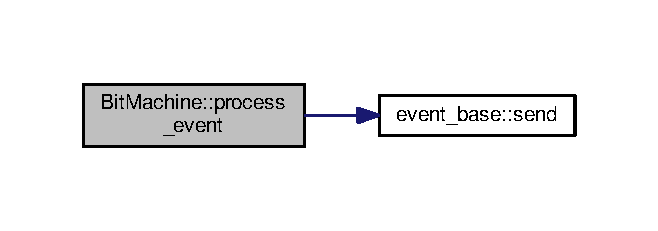
\includegraphics[width=316pt]{struct_bit_machine_ae77e5375e470002e98bde6307793b102_cgraph}
\end{center}
\end{figure}
Here is the caller graph for this function\+:
\nopagebreak
\begin{figure}[H]
\begin{center}
\leavevmode
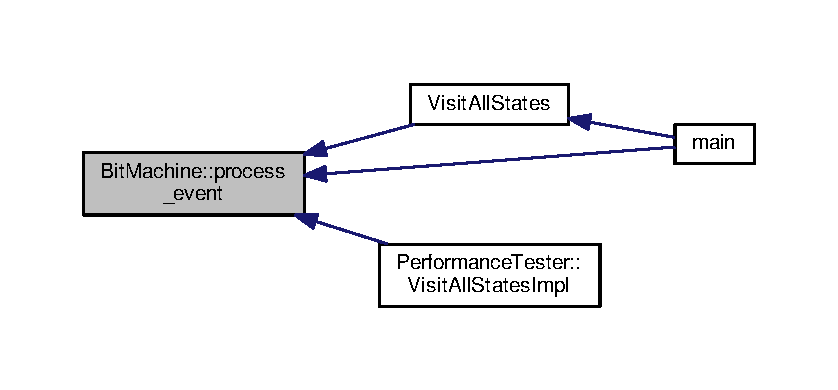
\includegraphics[width=350pt]{struct_bit_machine_ae77e5375e470002e98bde6307793b102_icgraph}
\end{center}
\end{figure}
\mbox{\Hypertarget{struct_bit_machine_a43a10ef23aab14065277c1bc34d08007}\label{struct_bit_machine_a43a10ef23aab14065277c1bc34d08007}} 
\index{Bit\+Machine@{Bit\+Machine}!Transition@{Transition}}
\index{Transition@{Transition}!Bit\+Machine@{Bit\+Machine}}
\subsubsection{\texorpdfstring{Transition()}{Transition()}\hspace{0.1cm}{\footnotesize\ttfamily [1/10]}}
{\footnotesize\ttfamily template$<$class No\+Of\+Bits, class First\+Transition\+Bit$>$ \\
void \mbox{\hyperlink{struct_bit_machine}{Bit\+Machine}}$<$ No\+Of\+Bits, First\+Transition\+Bit $>$\+::Transition (\begin{DoxyParamCaption}\item[{const \mbox{\hyperlink{struct_ev_flip_bit}{Ev\+Flip\+Bit}}$<$ \mbox{\hyperlink{_performance_8cpp_ac4323a4a68daf3126a7be25628f1d622}{uint0}} $>$ \&}]{ }\end{DoxyParamCaption})\hspace{0.3cm}{\ttfamily [inline]}}

\mbox{\Hypertarget{struct_bit_machine_a75b74e2bcb9417cad75dabe92e4663fc}\label{struct_bit_machine_a75b74e2bcb9417cad75dabe92e4663fc}} 
\index{Bit\+Machine@{Bit\+Machine}!Transition@{Transition}}
\index{Transition@{Transition}!Bit\+Machine@{Bit\+Machine}}
\subsubsection{\texorpdfstring{Transition()}{Transition()}\hspace{0.1cm}{\footnotesize\ttfamily [2/10]}}
{\footnotesize\ttfamily template$<$class No\+Of\+Bits, class First\+Transition\+Bit$>$ \\
void \mbox{\hyperlink{struct_bit_machine}{Bit\+Machine}}$<$ No\+Of\+Bits, First\+Transition\+Bit $>$\+::Transition (\begin{DoxyParamCaption}\item[{const \mbox{\hyperlink{struct_ev_flip_bit}{Ev\+Flip\+Bit}}$<$ \mbox{\hyperlink{_performance_8cpp_afada4030cdd8c9628ca412e4409d07d1}{uint1}} $>$ \&}]{ }\end{DoxyParamCaption})\hspace{0.3cm}{\ttfamily [inline]}}

\mbox{\Hypertarget{struct_bit_machine_a0eef1a8ac436d26db1920032bc81186b}\label{struct_bit_machine_a0eef1a8ac436d26db1920032bc81186b}} 
\index{Bit\+Machine@{Bit\+Machine}!Transition@{Transition}}
\index{Transition@{Transition}!Bit\+Machine@{Bit\+Machine}}
\subsubsection{\texorpdfstring{Transition()}{Transition()}\hspace{0.1cm}{\footnotesize\ttfamily [3/10]}}
{\footnotesize\ttfamily template$<$class No\+Of\+Bits, class First\+Transition\+Bit$>$ \\
void \mbox{\hyperlink{struct_bit_machine}{Bit\+Machine}}$<$ No\+Of\+Bits, First\+Transition\+Bit $>$\+::Transition (\begin{DoxyParamCaption}\item[{const \mbox{\hyperlink{struct_ev_flip_bit}{Ev\+Flip\+Bit}}$<$ \mbox{\hyperlink{_performance_8cpp_ad7cf25dde7cbe398d57ed74b7109aaaa}{uint2}} $>$ \&}]{ }\end{DoxyParamCaption})\hspace{0.3cm}{\ttfamily [inline]}}

\mbox{\Hypertarget{struct_bit_machine_a065addd94fcc6c7046e700da2d170370}\label{struct_bit_machine_a065addd94fcc6c7046e700da2d170370}} 
\index{Bit\+Machine@{Bit\+Machine}!Transition@{Transition}}
\index{Transition@{Transition}!Bit\+Machine@{Bit\+Machine}}
\subsubsection{\texorpdfstring{Transition()}{Transition()}\hspace{0.1cm}{\footnotesize\ttfamily [4/10]}}
{\footnotesize\ttfamily template$<$class No\+Of\+Bits, class First\+Transition\+Bit$>$ \\
void \mbox{\hyperlink{struct_bit_machine}{Bit\+Machine}}$<$ No\+Of\+Bits, First\+Transition\+Bit $>$\+::Transition (\begin{DoxyParamCaption}\item[{const \mbox{\hyperlink{struct_ev_flip_bit}{Ev\+Flip\+Bit}}$<$ \mbox{\hyperlink{_performance_8cpp_a487e33775f12c3ab023e66546a69810f}{uint3}} $>$ \&}]{ }\end{DoxyParamCaption})\hspace{0.3cm}{\ttfamily [inline]}}

\mbox{\Hypertarget{struct_bit_machine_a7a095e344792b70a069ee44fbd6f2e3a}\label{struct_bit_machine_a7a095e344792b70a069ee44fbd6f2e3a}} 
\index{Bit\+Machine@{Bit\+Machine}!Transition@{Transition}}
\index{Transition@{Transition}!Bit\+Machine@{Bit\+Machine}}
\subsubsection{\texorpdfstring{Transition()}{Transition()}\hspace{0.1cm}{\footnotesize\ttfamily [5/10]}}
{\footnotesize\ttfamily template$<$class No\+Of\+Bits, class First\+Transition\+Bit$>$ \\
void \mbox{\hyperlink{struct_bit_machine}{Bit\+Machine}}$<$ No\+Of\+Bits, First\+Transition\+Bit $>$\+::Transition (\begin{DoxyParamCaption}\item[{const \mbox{\hyperlink{struct_ev_flip_bit}{Ev\+Flip\+Bit}}$<$ \mbox{\hyperlink{_performance_8cpp_aa143aaac7fcfe524f6f4f33cc878ae95}{uint4}} $>$ \&}]{ }\end{DoxyParamCaption})\hspace{0.3cm}{\ttfamily [inline]}}

\mbox{\Hypertarget{struct_bit_machine_a6ae4632116970d2f52185f71e086c37d}\label{struct_bit_machine_a6ae4632116970d2f52185f71e086c37d}} 
\index{Bit\+Machine@{Bit\+Machine}!Transition@{Transition}}
\index{Transition@{Transition}!Bit\+Machine@{Bit\+Machine}}
\subsubsection{\texorpdfstring{Transition()}{Transition()}\hspace{0.1cm}{\footnotesize\ttfamily [6/10]}}
{\footnotesize\ttfamily template$<$class No\+Of\+Bits, class First\+Transition\+Bit$>$ \\
void \mbox{\hyperlink{struct_bit_machine}{Bit\+Machine}}$<$ No\+Of\+Bits, First\+Transition\+Bit $>$\+::Transition (\begin{DoxyParamCaption}\item[{const \mbox{\hyperlink{struct_ev_flip_bit}{Ev\+Flip\+Bit}}$<$ \mbox{\hyperlink{_performance_8cpp_a34732dbaa46d46251e4ac1faef9fcecd}{uint5}} $>$ \&}]{ }\end{DoxyParamCaption})\hspace{0.3cm}{\ttfamily [inline]}}

\mbox{\Hypertarget{struct_bit_machine_aa139bb8076c9041eae686111879dbdd1}\label{struct_bit_machine_aa139bb8076c9041eae686111879dbdd1}} 
\index{Bit\+Machine@{Bit\+Machine}!Transition@{Transition}}
\index{Transition@{Transition}!Bit\+Machine@{Bit\+Machine}}
\subsubsection{\texorpdfstring{Transition()}{Transition()}\hspace{0.1cm}{\footnotesize\ttfamily [7/10]}}
{\footnotesize\ttfamily template$<$class No\+Of\+Bits, class First\+Transition\+Bit$>$ \\
void \mbox{\hyperlink{struct_bit_machine}{Bit\+Machine}}$<$ No\+Of\+Bits, First\+Transition\+Bit $>$\+::Transition (\begin{DoxyParamCaption}\item[{const \mbox{\hyperlink{struct_ev_flip_bit}{Ev\+Flip\+Bit}}$<$ \mbox{\hyperlink{_performance_8cpp_a76e4a9cf398589b4ad27852c9f4389f9}{uint6}} $>$ \&}]{ }\end{DoxyParamCaption})\hspace{0.3cm}{\ttfamily [inline]}}

\mbox{\Hypertarget{struct_bit_machine_a006a8fcc19034fae402a95505f3ccafe}\label{struct_bit_machine_a006a8fcc19034fae402a95505f3ccafe}} 
\index{Bit\+Machine@{Bit\+Machine}!Transition@{Transition}}
\index{Transition@{Transition}!Bit\+Machine@{Bit\+Machine}}
\subsubsection{\texorpdfstring{Transition()}{Transition()}\hspace{0.1cm}{\footnotesize\ttfamily [8/10]}}
{\footnotesize\ttfamily template$<$class No\+Of\+Bits, class First\+Transition\+Bit$>$ \\
void \mbox{\hyperlink{struct_bit_machine}{Bit\+Machine}}$<$ No\+Of\+Bits, First\+Transition\+Bit $>$\+::Transition (\begin{DoxyParamCaption}\item[{const \mbox{\hyperlink{struct_ev_flip_bit}{Ev\+Flip\+Bit}}$<$ \mbox{\hyperlink{_performance_8cpp_ae332b751ff9ebef63d125fdaaaf45f8c}{uint7}} $>$ \&}]{ }\end{DoxyParamCaption})\hspace{0.3cm}{\ttfamily [inline]}}

\mbox{\Hypertarget{struct_bit_machine_a1ee9e973bde376f8b952b6ad14b6b246}\label{struct_bit_machine_a1ee9e973bde376f8b952b6ad14b6b246}} 
\index{Bit\+Machine@{Bit\+Machine}!Transition@{Transition}}
\index{Transition@{Transition}!Bit\+Machine@{Bit\+Machine}}
\subsubsection{\texorpdfstring{Transition()}{Transition()}\hspace{0.1cm}{\footnotesize\ttfamily [9/10]}}
{\footnotesize\ttfamily template$<$class No\+Of\+Bits, class First\+Transition\+Bit$>$ \\
void \mbox{\hyperlink{struct_bit_machine}{Bit\+Machine}}$<$ No\+Of\+Bits, First\+Transition\+Bit $>$\+::Transition (\begin{DoxyParamCaption}\item[{const \mbox{\hyperlink{struct_ev_flip_bit}{Ev\+Flip\+Bit}}$<$ \mbox{\hyperlink{_performance_8cpp_acf7191ac01fae99fae3f5a89e4f8a8ff}{uint8}} $>$ \&}]{ }\end{DoxyParamCaption})\hspace{0.3cm}{\ttfamily [inline]}}

\mbox{\Hypertarget{struct_bit_machine_a3ef5a60f15cd15bb46b63d2a86594c5a}\label{struct_bit_machine_a3ef5a60f15cd15bb46b63d2a86594c5a}} 
\index{Bit\+Machine@{Bit\+Machine}!Transition@{Transition}}
\index{Transition@{Transition}!Bit\+Machine@{Bit\+Machine}}
\subsubsection{\texorpdfstring{Transition()}{Transition()}\hspace{0.1cm}{\footnotesize\ttfamily [10/10]}}
{\footnotesize\ttfamily template$<$class No\+Of\+Bits, class First\+Transition\+Bit$>$ \\
void \mbox{\hyperlink{struct_bit_machine}{Bit\+Machine}}$<$ No\+Of\+Bits, First\+Transition\+Bit $>$\+::Transition (\begin{DoxyParamCaption}\item[{const \mbox{\hyperlink{struct_ev_flip_bit}{Ev\+Flip\+Bit}}$<$ \mbox{\hyperlink{_performance_8cpp_ac1d5f5aee5a76e77d960741a1bd84b12}{uint9}} $>$ \&}]{ }\end{DoxyParamCaption})\hspace{0.3cm}{\ttfamily [inline]}}



\subsection{Member Data Documentation}
\mbox{\Hypertarget{struct_bit_machine_ad35b2868f25bc77b9b9db1f1e9d03c8b}\label{struct_bit_machine_ad35b2868f25bc77b9b9db1f1e9d03c8b}} 
\index{Bit\+Machine@{Bit\+Machine}!in\+State\+Reactions\+\_\+@{in\+State\+Reactions\+\_\+}}
\index{in\+State\+Reactions\+\_\+@{in\+State\+Reactions\+\_\+}!Bit\+Machine@{Bit\+Machine}}
\subsubsection{\texorpdfstring{in\+State\+Reactions\+\_\+}{inStateReactions\_}}
{\footnotesize\ttfamily template$<$class No\+Of\+Bits, class First\+Transition\+Bit$>$ \\
unsigned int \mbox{\hyperlink{struct_bit_machine}{Bit\+Machine}}$<$ No\+Of\+Bits, First\+Transition\+Bit $>$\+::in\+State\+Reactions\+\_\+\hspace{0.3cm}{\ttfamily [private]}}

\mbox{\Hypertarget{struct_bit_machine_a22ecd751130c63597ce80ca5c1d9bff3}\label{struct_bit_machine_a22ecd751130c63597ce80ca5c1d9bff3}} 
\index{Bit\+Machine@{Bit\+Machine}!p\+Current\+State\+\_\+@{p\+Current\+State\+\_\+}}
\index{p\+Current\+State\+\_\+@{p\+Current\+State\+\_\+}!Bit\+Machine@{Bit\+Machine}}
\subsubsection{\texorpdfstring{p\+Current\+State\+\_\+}{pCurrentState\_}}
{\footnotesize\ttfamily template$<$class No\+Of\+Bits, class First\+Transition\+Bit$>$ \\
const \mbox{\hyperlink{classstate__base}{state\+\_\+base}}$\ast$ \mbox{\hyperlink{struct_bit_machine}{Bit\+Machine}}$<$ No\+Of\+Bits, First\+Transition\+Bit $>$\+::p\+Current\+State\+\_\+\hspace{0.3cm}{\ttfamily [private]}}

\mbox{\Hypertarget{struct_bit_machine_a042875c3dcc1ff444ddd45df5ca47c56}\label{struct_bit_machine_a042875c3dcc1ff444ddd45df5ca47c56}} 
\index{Bit\+Machine@{Bit\+Machine}!transitions\+\_\+@{transitions\+\_\+}}
\index{transitions\+\_\+@{transitions\+\_\+}!Bit\+Machine@{Bit\+Machine}}
\subsubsection{\texorpdfstring{transitions\+\_\+}{transitions\_}}
{\footnotesize\ttfamily template$<$class No\+Of\+Bits, class First\+Transition\+Bit$>$ \\
unsigned int \mbox{\hyperlink{struct_bit_machine}{Bit\+Machine}}$<$ No\+Of\+Bits, First\+Transition\+Bit $>$\+::transitions\+\_\+\hspace{0.3cm}{\ttfamily [private]}}



The documentation for this struct was generated from the following files\+:\begin{DoxyCompactItemize}
\item 
example/\+Bit\+Machine/\mbox{\hyperlink{_bit_machine_8cpp}{Bit\+Machine.\+cpp}}\item 
example/\+Handcrafted/\mbox{\hyperlink{_handcrafted_8cpp}{Handcrafted.\+cpp}}\item 
example/\+Performance/\mbox{\hyperlink{_performance_8cpp}{Performance.\+cpp}}\end{DoxyCompactItemize}

\hypertarget{struct_bit_state}{}\section{Bit\+State$<$ State\+No, No\+Of\+Bits, First\+Transition\+Bit $>$ Struct Template Reference}
\label{struct_bit_state}\index{Bit\+State$<$ State\+No, No\+Of\+Bits, First\+Transition\+Bit $>$@{Bit\+State$<$ State\+No, No\+Of\+Bits, First\+Transition\+Bit $>$}}


Inheritance diagram for Bit\+State$<$ State\+No, No\+Of\+Bits, First\+Transition\+Bit $>$\+:
\nopagebreak
\begin{figure}[H]
\begin{center}
\leavevmode
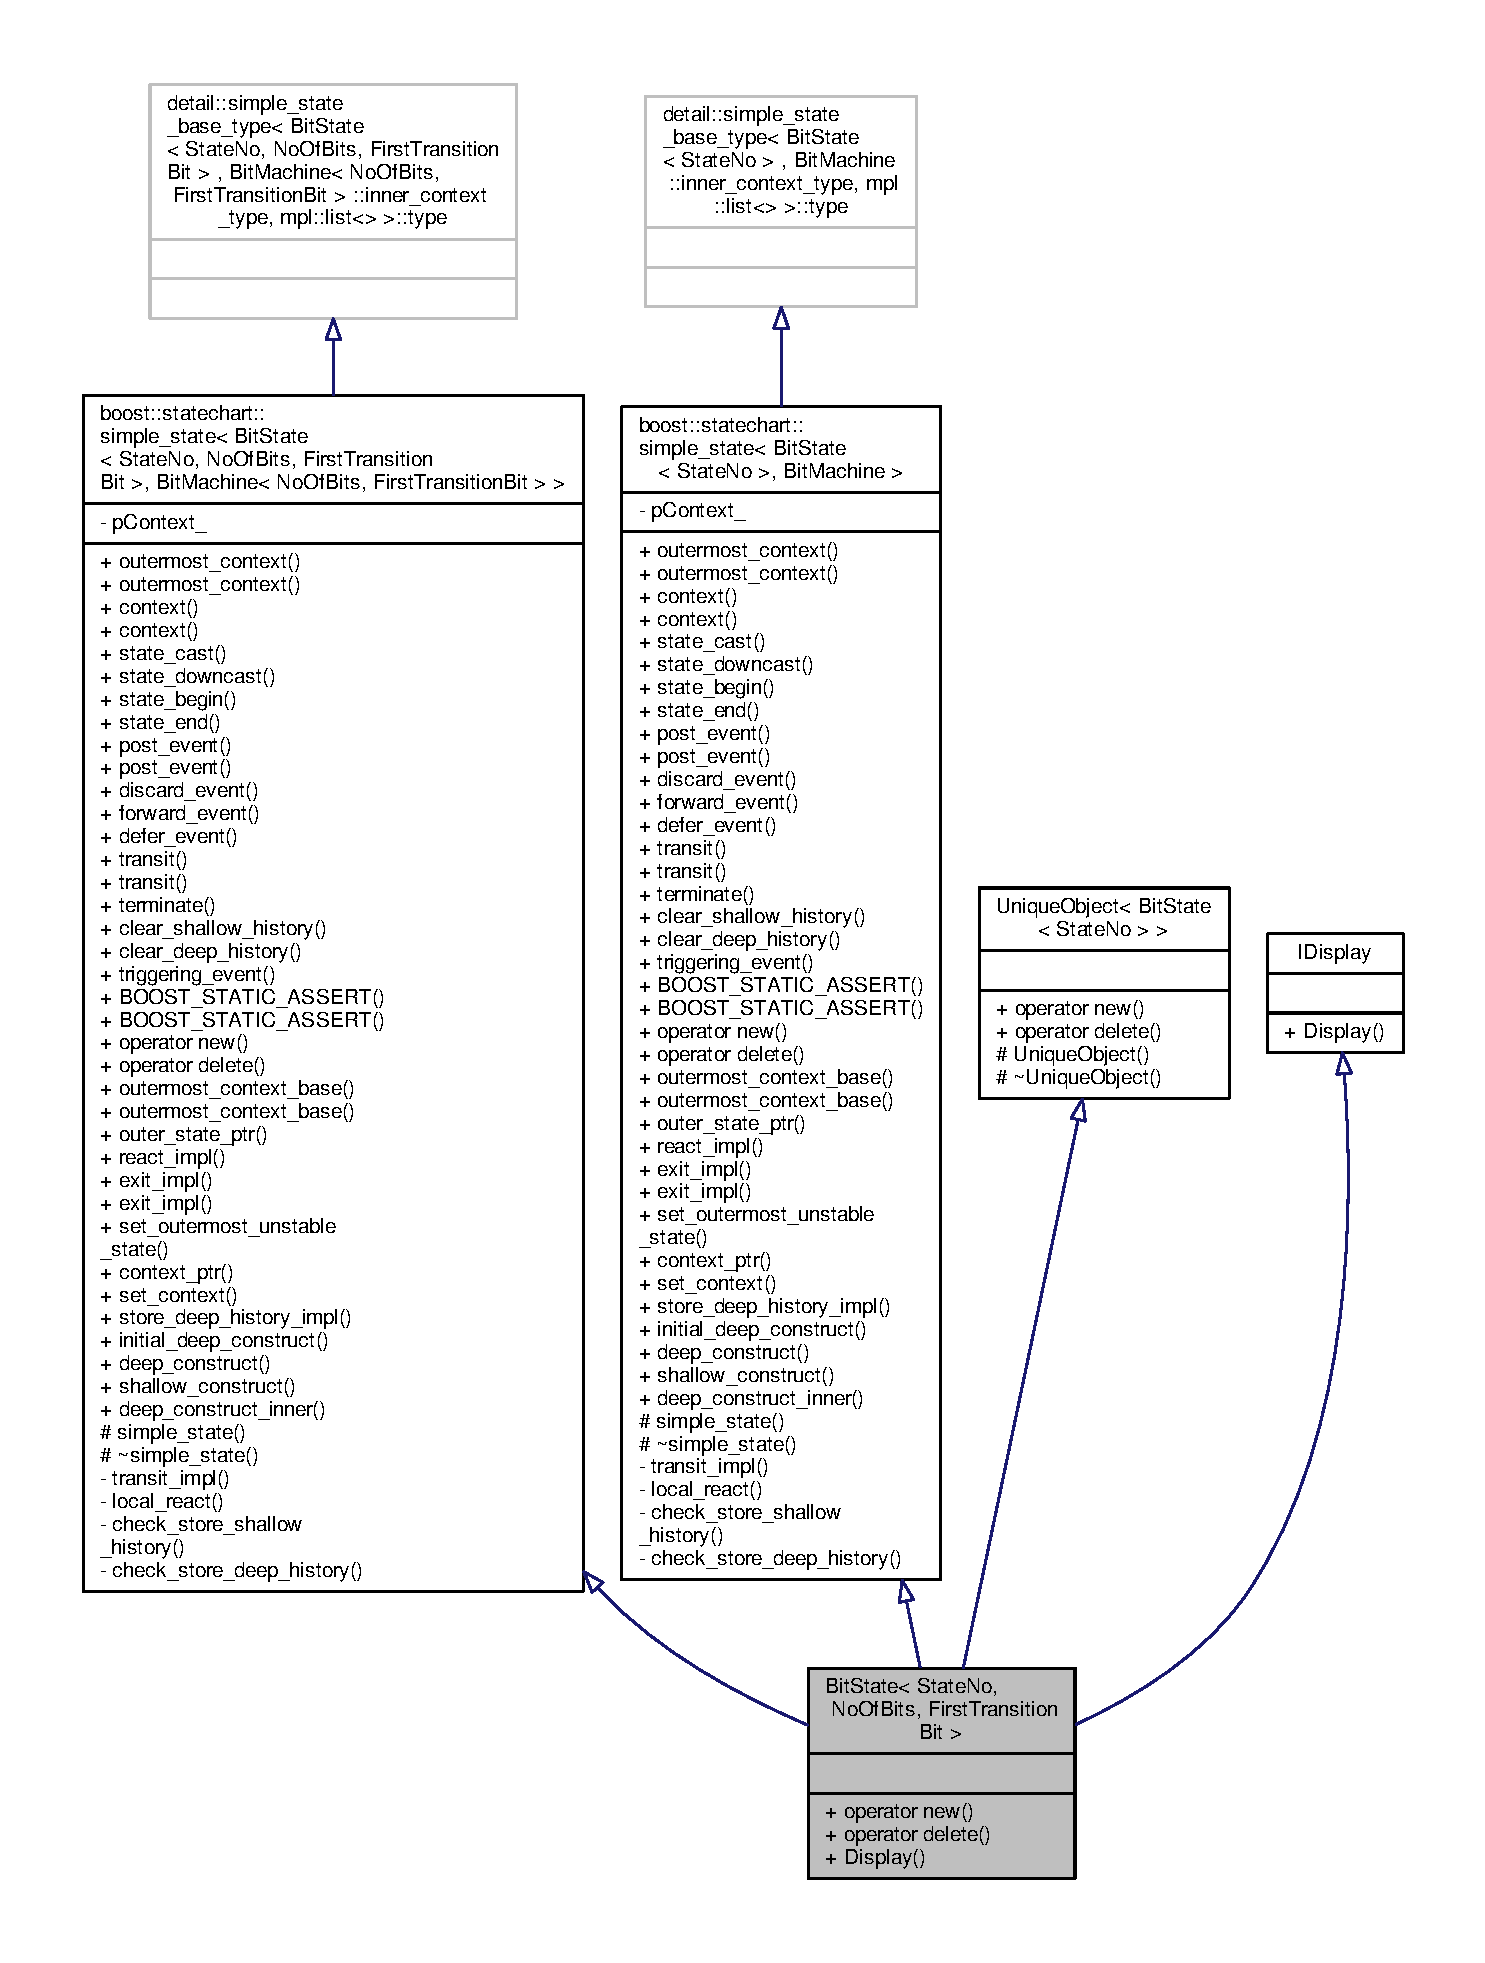
\includegraphics[width=350pt]{struct_bit_state__inherit__graph}
\end{center}
\end{figure}


Collaboration diagram for Bit\+State$<$ State\+No, No\+Of\+Bits, First\+Transition\+Bit $>$\+:
\nopagebreak
\begin{figure}[H]
\begin{center}
\leavevmode
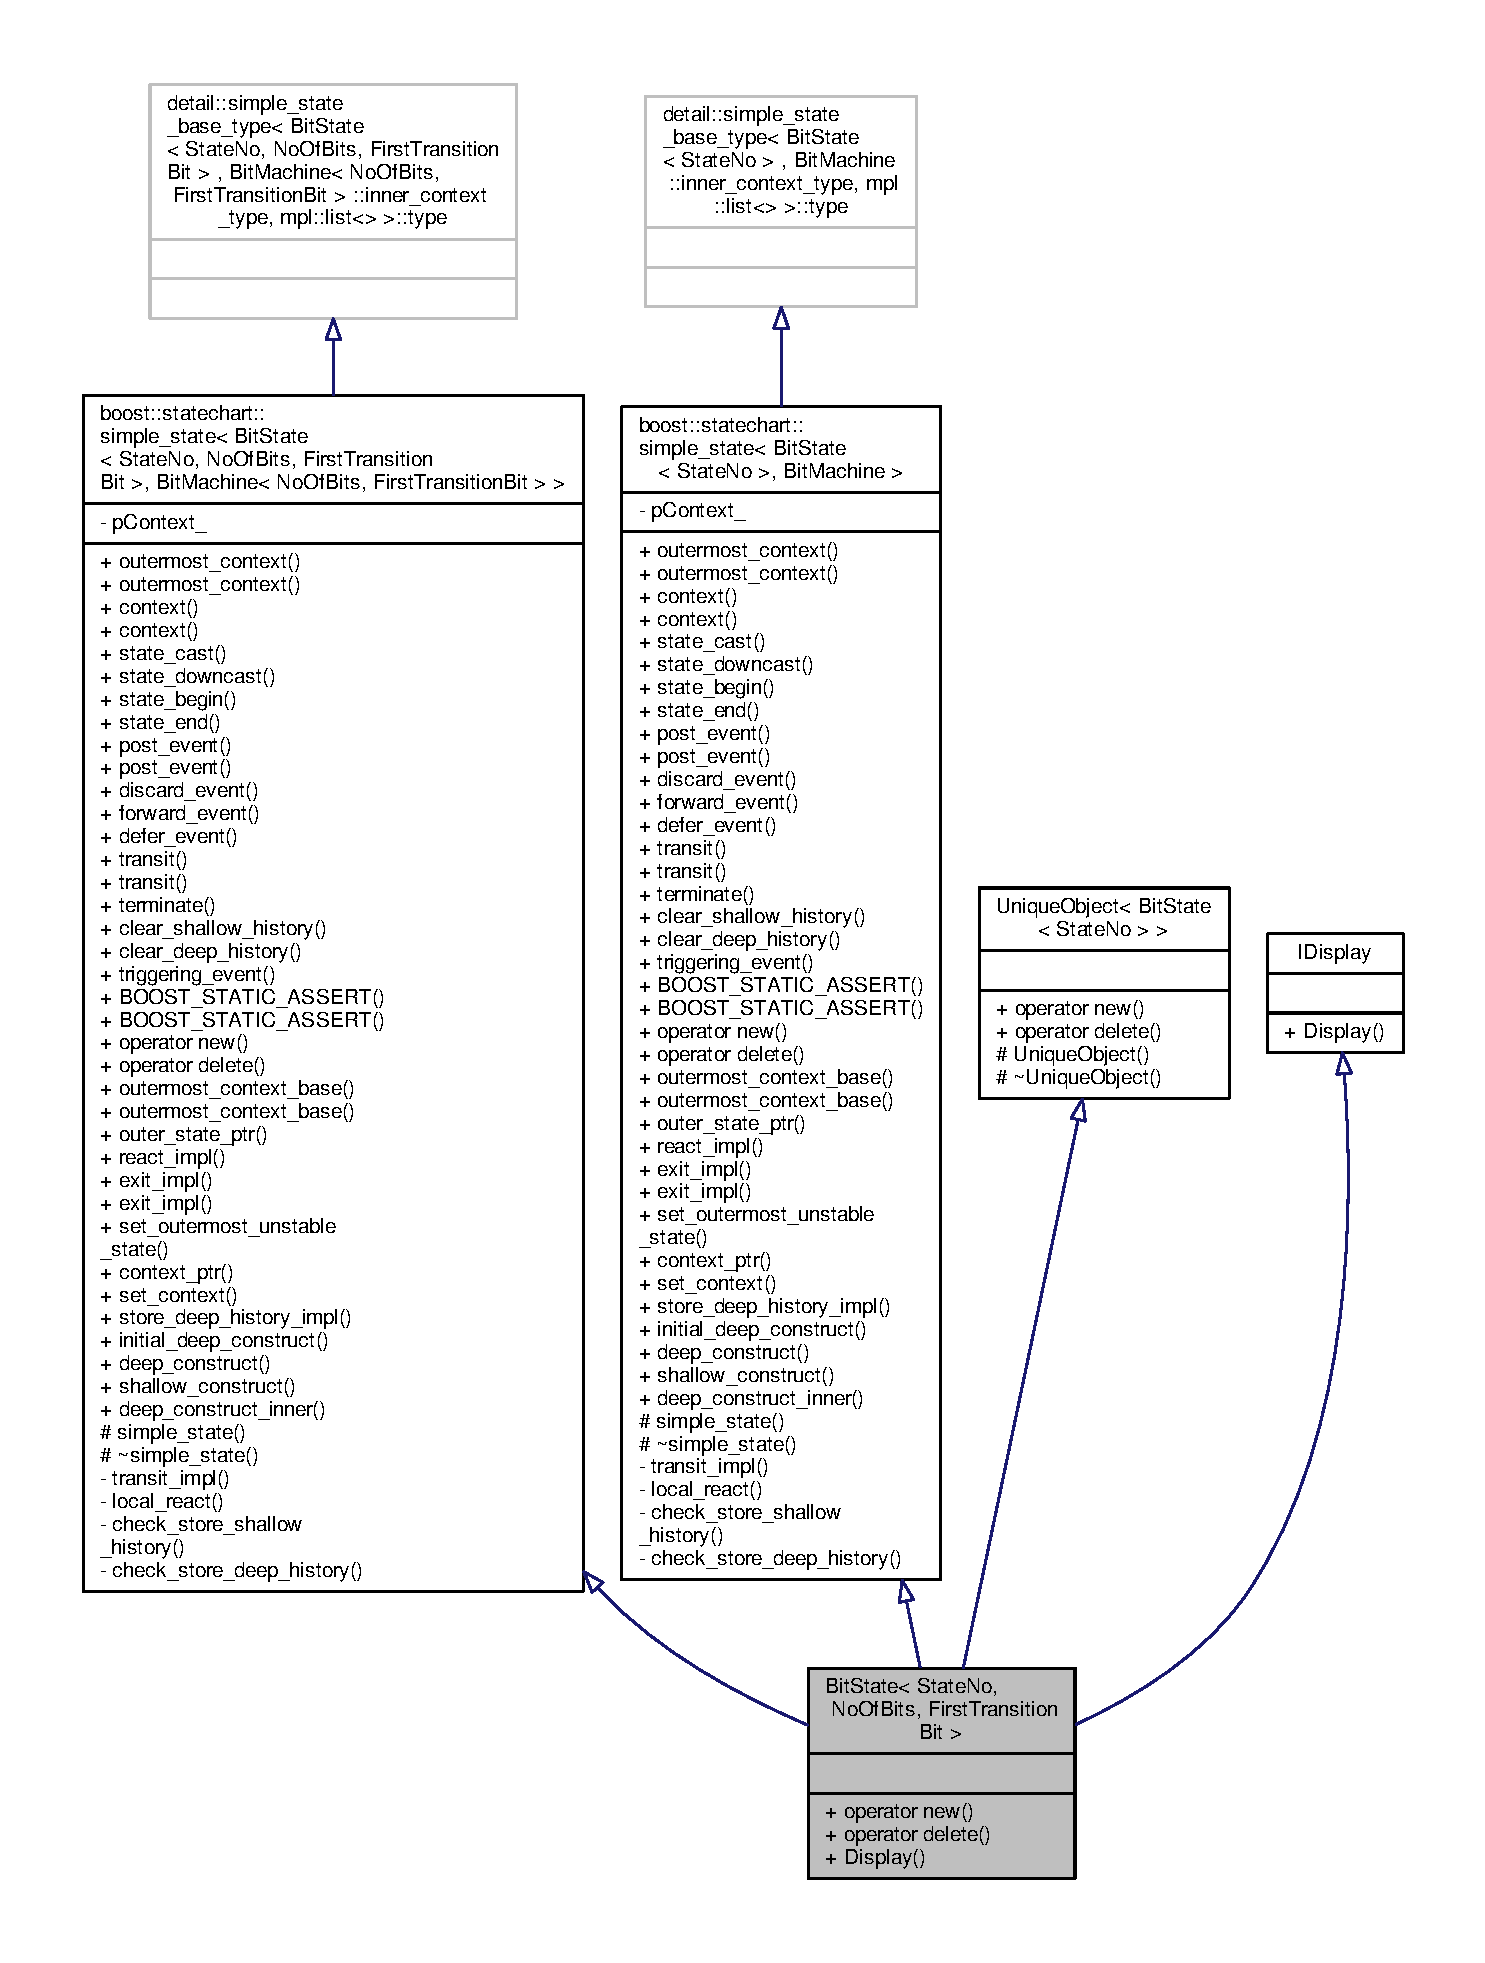
\includegraphics[width=350pt]{struct_bit_state__coll__graph}
\end{center}
\end{figure}
\subsection*{Public Types}
\begin{DoxyCompactItemize}
\item 
typedef mpl\+::copy$<$ typename mpl\+::transform\+\_\+view$<$ mpl\+::range\+\_\+c$<$ unsigned int, 0, \mbox{\hyperlink{_bit_machine_8cpp_ac894b74325002b036bfc596bd5434f89}{N\+O\+\_\+\+O\+F\+\_\+\+B\+I\+TS}} $>$, \mbox{\hyperlink{struct_flip_transition}{Flip\+Transition}}$<$ mpl\+::placeholders\+::\+\_\+, State\+No $>$ $>$\+::type, mpl\+::front\+\_\+inserter$<$ mpl\+::list$<$$>$ $>$ $>$\+::type \mbox{\hyperlink{struct_bit_state_a59bd125c7d205880081926b1a6d7689a}{reactions}}
\item 
typedef mpl\+::copy$<$ typename mpl\+::transform\+\_\+view$<$ mpl\+::range\+\_\+c$<$ unsigned int, 0, No\+Of\+Bits\+::value $>$, \mbox{\hyperlink{struct_flip_transition}{Flip\+Transition}}$<$ mpl\+::placeholders\+::\+\_\+, State\+No, No\+Of\+Bits, First\+Transition\+Bit $>$ $>$\+::type, mpl\+::front\+\_\+inserter$<$ mpl\+::list$<$$>$ $>$ $>$\+::type \mbox{\hyperlink{struct_bit_state_a409080fdeaba7f3ec0b63f44bc683d92}{reactions}}
\end{DoxyCompactItemize}
\subsection*{Public Member Functions}
\begin{DoxyCompactItemize}
\item 
void $\ast$ \mbox{\hyperlink{struct_bit_state_aa7543c5a18aa027866b17e5fe389a413}{operator new}} (std\+::size\+\_\+t size)
\item 
void \mbox{\hyperlink{struct_bit_state_ac0109e89bbccfb21a812a92b239ebac2}{operator delete}} (void $\ast$p, std\+::size\+\_\+t size)
\item 
virtual void \mbox{\hyperlink{struct_bit_state_a3f26c599cf4a72a263d4fc2c2f7e693d}{Display}} () const
\end{DoxyCompactItemize}
\subsection*{Additional Inherited Members}


\subsection{Member Typedef Documentation}
\mbox{\Hypertarget{struct_bit_state_a59bd125c7d205880081926b1a6d7689a}\label{struct_bit_state_a59bd125c7d205880081926b1a6d7689a}} 
\index{Bit\+State@{Bit\+State}!reactions@{reactions}}
\index{reactions@{reactions}!Bit\+State@{Bit\+State}}
\subsubsection{\texorpdfstring{reactions}{reactions}\hspace{0.1cm}{\footnotesize\ttfamily [1/2]}}
{\footnotesize\ttfamily template$<$class State\+No , class No\+Of\+Bits , class First\+Transition\+Bit $>$ \\
typedef mpl\+::copy$<$ typename mpl\+::transform\+\_\+view$<$ mpl\+::range\+\_\+c$<$ unsigned int, 0, \mbox{\hyperlink{_bit_machine_8cpp_ac894b74325002b036bfc596bd5434f89}{N\+O\+\_\+\+O\+F\+\_\+\+B\+I\+TS}} $>$, \mbox{\hyperlink{struct_flip_transition}{Flip\+Transition}}$<$ mpl\+::placeholders\+::\+\_\+, State\+No $>$ $>$\+::type, mpl\+::front\+\_\+inserter$<$ mpl\+::list$<$$>$ $>$ $>$\+::type \mbox{\hyperlink{struct_bit_state}{Bit\+State}}$<$ State\+No, No\+Of\+Bits, First\+Transition\+Bit $>$\+::\mbox{\hyperlink{struct_bit_state_a59bd125c7d205880081926b1a6d7689a}{reactions}}}

\mbox{\Hypertarget{struct_bit_state_a409080fdeaba7f3ec0b63f44bc683d92}\label{struct_bit_state_a409080fdeaba7f3ec0b63f44bc683d92}} 
\index{Bit\+State@{Bit\+State}!reactions@{reactions}}
\index{reactions@{reactions}!Bit\+State@{Bit\+State}}
\subsubsection{\texorpdfstring{reactions}{reactions}\hspace{0.1cm}{\footnotesize\ttfamily [2/2]}}
{\footnotesize\ttfamily template$<$class State\+No , class No\+Of\+Bits , class First\+Transition\+Bit $>$ \\
typedef mpl\+::copy$<$ typename mpl\+::transform\+\_\+view$<$ mpl\+::range\+\_\+c$<$ unsigned int, 0, No\+Of\+Bits\+::value $>$, \mbox{\hyperlink{struct_flip_transition}{Flip\+Transition}}$<$ mpl\+::placeholders\+::\+\_\+, State\+No, No\+Of\+Bits, First\+Transition\+Bit $>$ $>$\+::type, mpl\+::front\+\_\+inserter$<$ mpl\+::list$<$$>$ $>$ $>$\+::type \mbox{\hyperlink{struct_bit_state}{Bit\+State}}$<$ State\+No, No\+Of\+Bits, First\+Transition\+Bit $>$\+::\mbox{\hyperlink{struct_bit_state_a59bd125c7d205880081926b1a6d7689a}{reactions}}}



\subsection{Member Function Documentation}
\mbox{\Hypertarget{struct_bit_state_a3f26c599cf4a72a263d4fc2c2f7e693d}\label{struct_bit_state_a3f26c599cf4a72a263d4fc2c2f7e693d}} 
\index{Bit\+State@{Bit\+State}!Display@{Display}}
\index{Display@{Display}!Bit\+State@{Bit\+State}}
\subsubsection{\texorpdfstring{Display()}{Display()}}
{\footnotesize\ttfamily template$<$class State\+No , class No\+Of\+Bits , class First\+Transition\+Bit $>$ \\
virtual void \mbox{\hyperlink{struct_bit_state}{Bit\+State}}$<$ State\+No, No\+Of\+Bits, First\+Transition\+Bit $>$\+::Display (\begin{DoxyParamCaption}{ }\end{DoxyParamCaption}) const\hspace{0.3cm}{\ttfamily [inline]}, {\ttfamily [virtual]}}



Implements \mbox{\hyperlink{struct_i_display_a661bdbd2f3b46f7e0d8f8211a212f184}{I\+Display}}.

Here is the call graph for this function\+:
\nopagebreak
\begin{figure}[H]
\begin{center}
\leavevmode
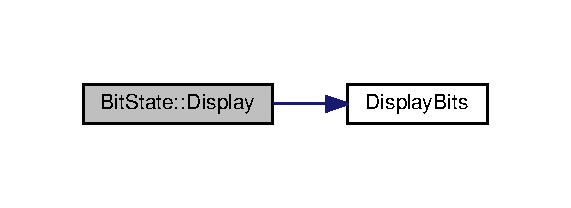
\includegraphics[width=274pt]{struct_bit_state_a3f26c599cf4a72a263d4fc2c2f7e693d_cgraph}
\end{center}
\end{figure}
\mbox{\Hypertarget{struct_bit_state_ac0109e89bbccfb21a812a92b239ebac2}\label{struct_bit_state_ac0109e89bbccfb21a812a92b239ebac2}} 
\index{Bit\+State@{Bit\+State}!operator delete@{operator delete}}
\index{operator delete@{operator delete}!Bit\+State@{Bit\+State}}
\subsubsection{\texorpdfstring{operator delete()}{operator delete()}}
{\footnotesize\ttfamily template$<$class State\+No , class No\+Of\+Bits , class First\+Transition\+Bit $>$ \\
void \mbox{\hyperlink{struct_bit_state}{Bit\+State}}$<$ State\+No, No\+Of\+Bits, First\+Transition\+Bit $>$\+::operator delete (\begin{DoxyParamCaption}\item[{void $\ast$}]{p,  }\item[{std\+::size\+\_\+t}]{size }\end{DoxyParamCaption})\hspace{0.3cm}{\ttfamily [inline]}}

\mbox{\Hypertarget{struct_bit_state_aa7543c5a18aa027866b17e5fe389a413}\label{struct_bit_state_aa7543c5a18aa027866b17e5fe389a413}} 
\index{Bit\+State@{Bit\+State}!operator new@{operator new}}
\index{operator new@{operator new}!Bit\+State@{Bit\+State}}
\subsubsection{\texorpdfstring{operator new()}{operator new()}}
{\footnotesize\ttfamily template$<$class State\+No , class No\+Of\+Bits , class First\+Transition\+Bit $>$ \\
void$\ast$ \mbox{\hyperlink{struct_bit_state}{Bit\+State}}$<$ State\+No, No\+Of\+Bits, First\+Transition\+Bit $>$\+::operator new (\begin{DoxyParamCaption}\item[{std\+::size\+\_\+t}]{size }\end{DoxyParamCaption})\hspace{0.3cm}{\ttfamily [inline]}}



The documentation for this struct was generated from the following files\+:\begin{DoxyCompactItemize}
\item 
example/\+Bit\+Machine/\mbox{\hyperlink{_bit_machine_8cpp}{Bit\+Machine.\+cpp}}\item 
example/\+Performance/\mbox{\hyperlink{_performance_8cpp}{Performance.\+cpp}}\end{DoxyCompactItemize}

\hypertarget{struct_c}{}\section{C Struct Reference}
\label{struct_c}\index{C@{C}}


Inheritance diagram for C\+:
\nopagebreak
\begin{figure}[H]
\begin{center}
\leavevmode
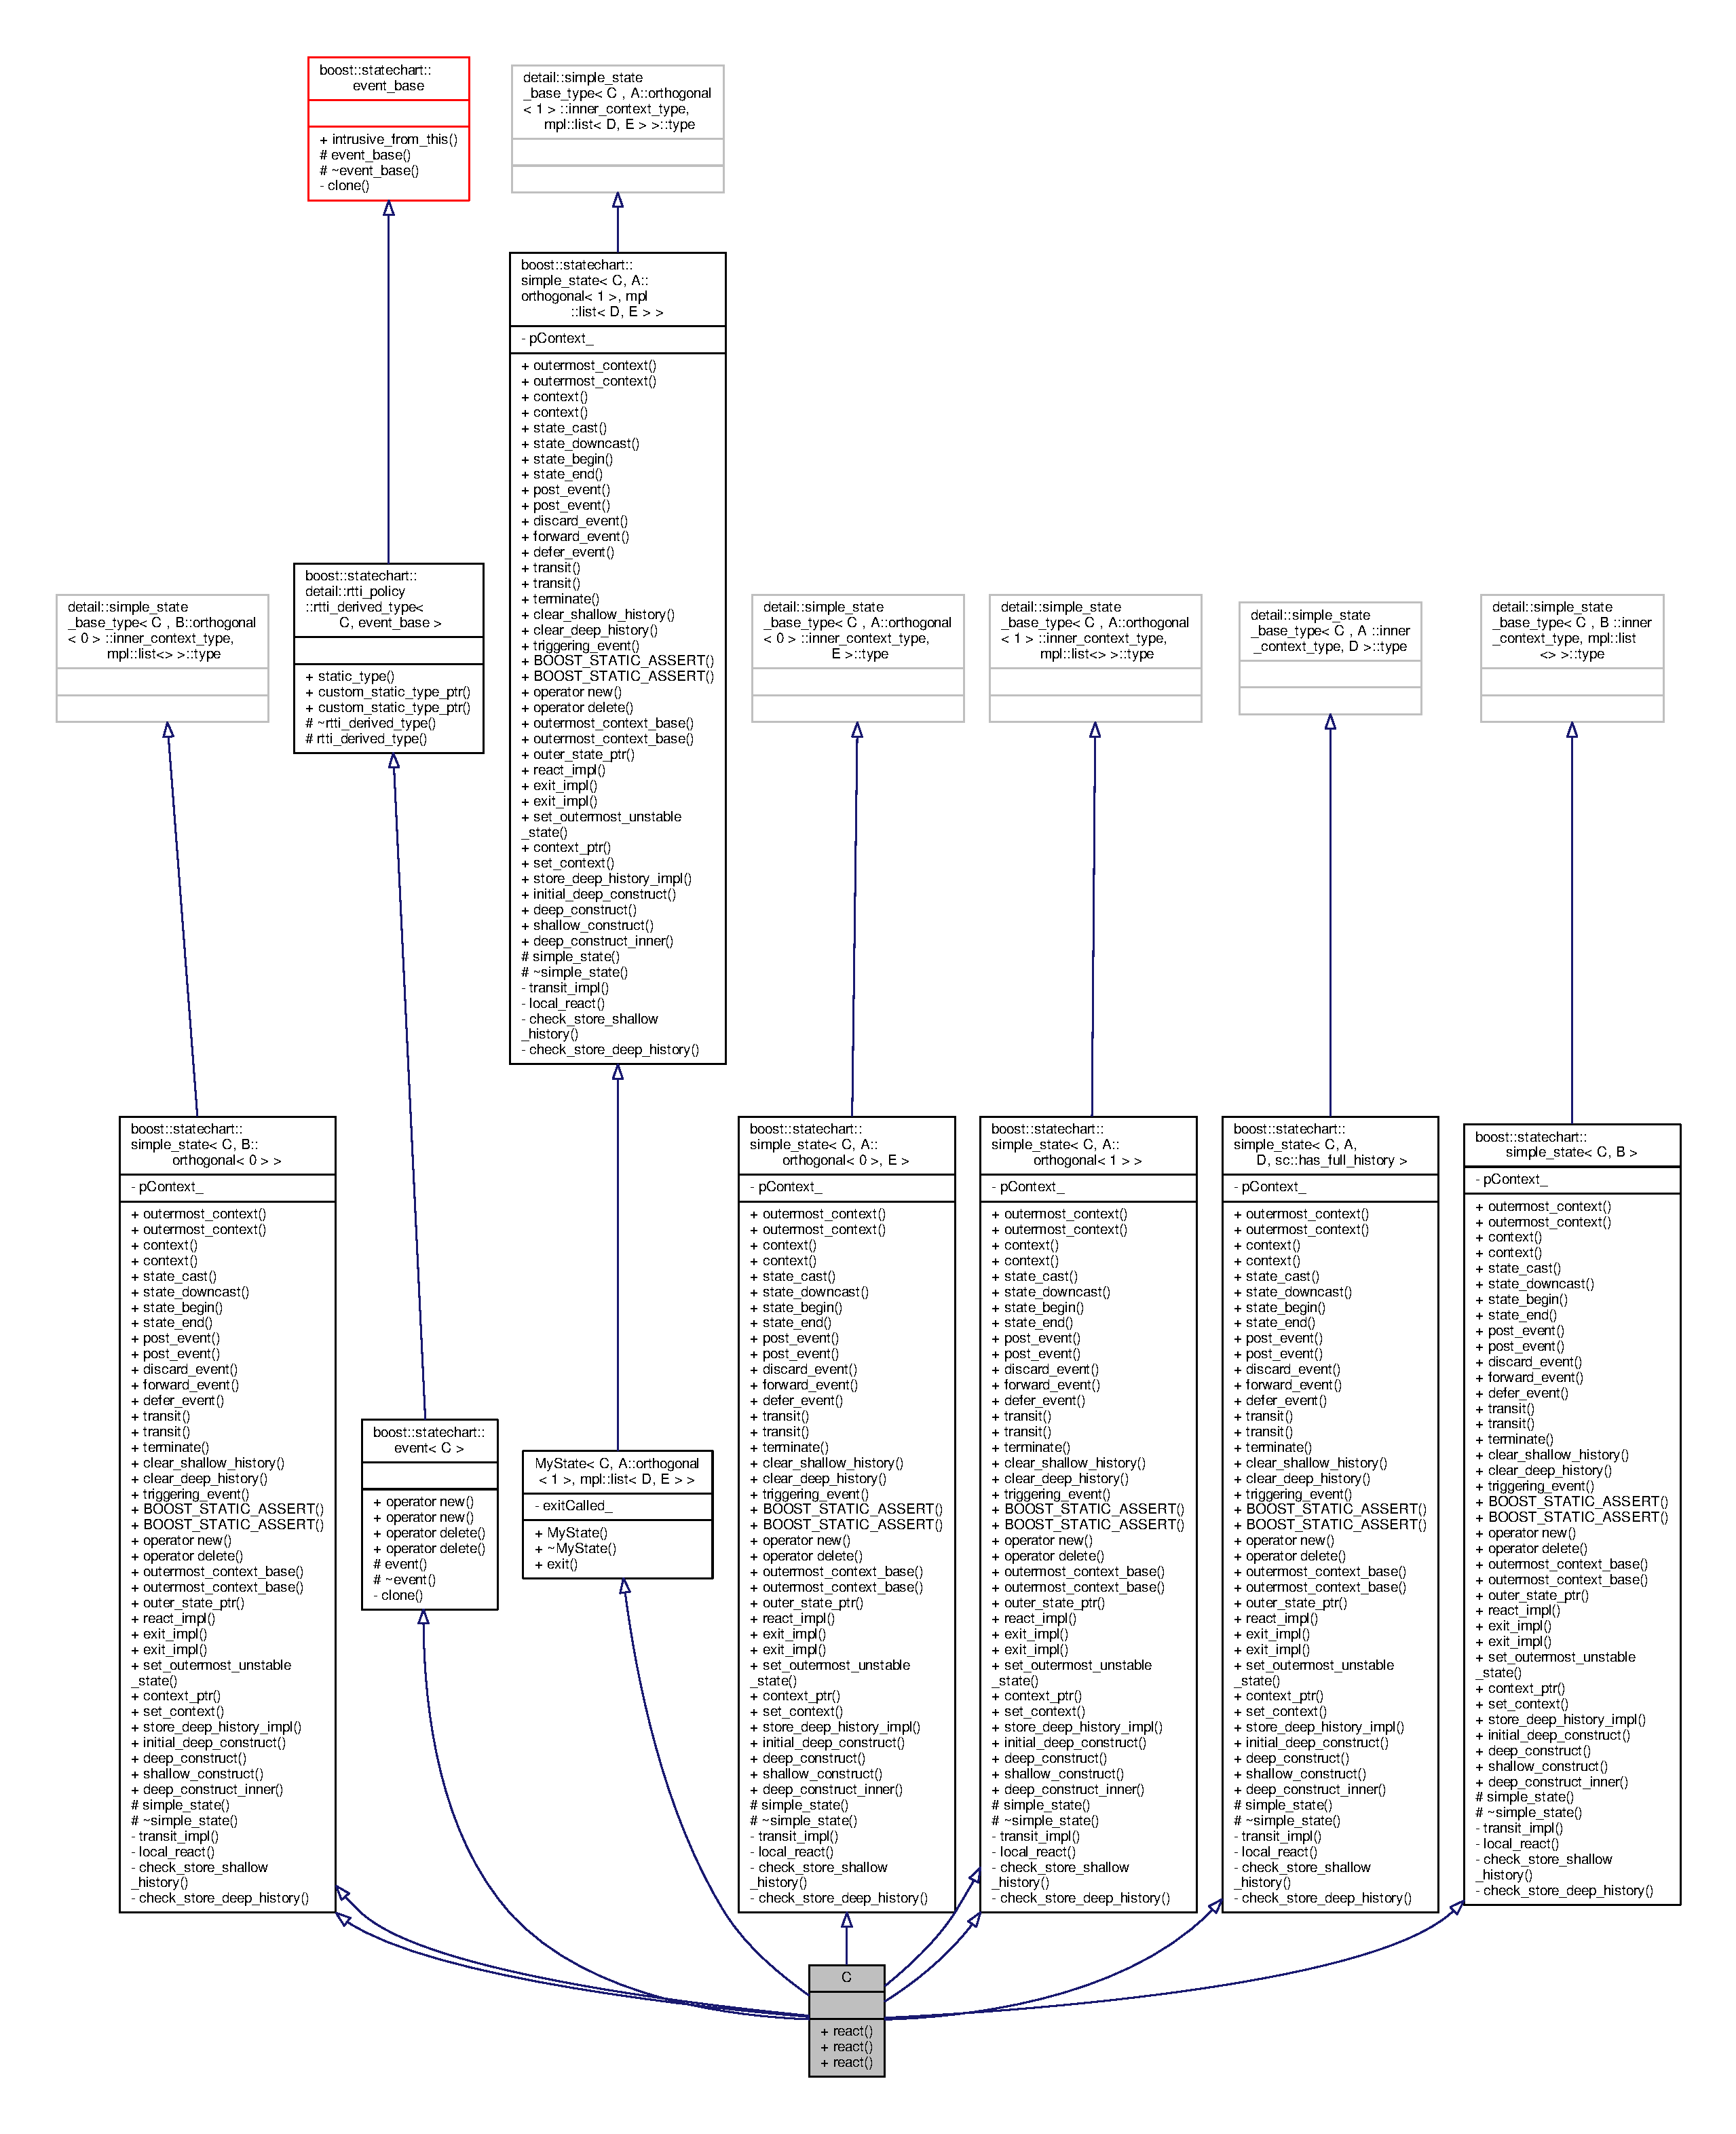
\includegraphics[width=350pt]{struct_c__inherit__graph}
\end{center}
\end{figure}


Collaboration diagram for C\+:
\nopagebreak
\begin{figure}[H]
\begin{center}
\leavevmode
\includegraphics[width=350pt]{struct_c__coll__graph}
\end{center}
\end{figure}
\subsection*{Public Types}
\begin{DoxyCompactItemize}
\item 
typedef mpl\+::list$<$ \mbox{\hyperlink{classboost_1_1statechart_1_1transition}{sc\+::transition}}$<$ \mbox{\hyperlink{struct_ev_to_d}{Ev\+ToD}}, \mbox{\hyperlink{struct_d}{D}} $>$, \mbox{\hyperlink{classboost_1_1statechart_1_1custom__reaction}{sc\+::custom\+\_\+reaction}}$<$ \mbox{\hyperlink{struct_ev_discard_never}{Ev\+Discard\+Never}} $>$, \mbox{\hyperlink{classboost_1_1statechart_1_1custom__reaction}{sc\+::custom\+\_\+reaction}}$<$ \mbox{\hyperlink{struct_ev_discard_in_b}{Ev\+Discard\+InB}} $>$, \mbox{\hyperlink{classboost_1_1statechart_1_1custom__reaction}{sc\+::custom\+\_\+reaction}}$<$ \mbox{\hyperlink{struct_ev_discard_in_d}{Ev\+Discard\+InD}} $>$ $>$ \mbox{\hyperlink{struct_c_a1891987db7cdbea5f19084087b9174fa}{reactions}}
\item 
typedef \mbox{\hyperlink{classboost_1_1statechart_1_1termination}{sc\+::termination}}$<$ \mbox{\hyperlink{struct_ev_terminate_c}{Ev\+TerminateC}} $>$ \mbox{\hyperlink{struct_c_ab8b632236e00c355feedf0213d217543}{reactions}}
\end{DoxyCompactItemize}
\subsection*{Public Member Functions}
\begin{DoxyCompactItemize}
\item 
\mbox{\hyperlink{namespaceboost_1_1statechart_abe807f6598b614d6d87bb951ecd92331}{sc\+::result}} \mbox{\hyperlink{struct_c_a7c66bc54e8f268346ec27933ad446d5d}{react}} (const \mbox{\hyperlink{struct_ev_discard_never}{Ev\+Discard\+Never}} \&)
\item 
\mbox{\hyperlink{namespaceboost_1_1statechart_abe807f6598b614d6d87bb951ecd92331}{sc\+::result}} \mbox{\hyperlink{struct_c_af44f3b580444ff4e97f803b18de14499}{react}} (const \mbox{\hyperlink{struct_ev_discard_in_b}{Ev\+Discard\+InB}} \&)
\item 
\mbox{\hyperlink{namespaceboost_1_1statechart_abe807f6598b614d6d87bb951ecd92331}{sc\+::result}} \mbox{\hyperlink{struct_c_ab564da3e047d017f15645aa4682ae8f3}{react}} (const \mbox{\hyperlink{struct_ev_discard_in_d}{Ev\+Discard\+InD}} \&)
\end{DoxyCompactItemize}
\subsection*{Additional Inherited Members}


\subsection{Member Typedef Documentation}
\mbox{\Hypertarget{struct_c_ab8b632236e00c355feedf0213d217543}\label{struct_c_ab8b632236e00c355feedf0213d217543}} 
\index{C@{C}!reactions@{reactions}}
\index{reactions@{reactions}!C@{C}}
\subsubsection{\texorpdfstring{reactions}{reactions}\hspace{0.1cm}{\footnotesize\ttfamily [1/2]}}
{\footnotesize\ttfamily typedef \mbox{\hyperlink{classboost_1_1statechart_1_1termination}{sc\+::termination}}$<$ \mbox{\hyperlink{struct_ev_terminate_c}{Ev\+TerminateC}} $>$ \mbox{\hyperlink{struct_c_a1891987db7cdbea5f19084087b9174fa}{C\+::reactions}}}

\mbox{\Hypertarget{struct_c_a1891987db7cdbea5f19084087b9174fa}\label{struct_c_a1891987db7cdbea5f19084087b9174fa}} 
\index{C@{C}!reactions@{reactions}}
\index{reactions@{reactions}!C@{C}}
\subsubsection{\texorpdfstring{reactions}{reactions}\hspace{0.1cm}{\footnotesize\ttfamily [2/2]}}
{\footnotesize\ttfamily typedef mpl\+::list$<$ \mbox{\hyperlink{classboost_1_1statechart_1_1transition}{sc\+::transition}}$<$ \mbox{\hyperlink{struct_ev_to_d}{Ev\+ToD}}, \mbox{\hyperlink{struct_d}{D}} $>$, \mbox{\hyperlink{classboost_1_1statechart_1_1custom__reaction}{sc\+::custom\+\_\+reaction}}$<$ \mbox{\hyperlink{struct_ev_discard_never}{Ev\+Discard\+Never}} $>$, \mbox{\hyperlink{classboost_1_1statechart_1_1custom__reaction}{sc\+::custom\+\_\+reaction}}$<$ \mbox{\hyperlink{struct_ev_discard_in_b}{Ev\+Discard\+InB}} $>$, \mbox{\hyperlink{classboost_1_1statechart_1_1custom__reaction}{sc\+::custom\+\_\+reaction}}$<$ \mbox{\hyperlink{struct_ev_discard_in_d}{Ev\+Discard\+InD}} $>$ $>$ \mbox{\hyperlink{struct_c_a1891987db7cdbea5f19084087b9174fa}{C\+::reactions}}}



\subsection{Member Function Documentation}
\mbox{\Hypertarget{struct_c_a7c66bc54e8f268346ec27933ad446d5d}\label{struct_c_a7c66bc54e8f268346ec27933ad446d5d}} 
\index{C@{C}!react@{react}}
\index{react@{react}!C@{C}}
\subsubsection{\texorpdfstring{react()}{react()}\hspace{0.1cm}{\footnotesize\ttfamily [1/3]}}
{\footnotesize\ttfamily \mbox{\hyperlink{namespaceboost_1_1statechart_abe807f6598b614d6d87bb951ecd92331}{sc\+::result}} C\+::react (\begin{DoxyParamCaption}\item[{const \mbox{\hyperlink{struct_ev_discard_never}{Ev\+Discard\+Never}} \&}]{ }\end{DoxyParamCaption})\hspace{0.3cm}{\ttfamily [inline]}}

Here is the call graph for this function\+:
\nopagebreak
\begin{figure}[H]
\begin{center}
\leavevmode
\includegraphics[width=278pt]{struct_c_a7c66bc54e8f268346ec27933ad446d5d_cgraph}
\end{center}
\end{figure}
\mbox{\Hypertarget{struct_c_af44f3b580444ff4e97f803b18de14499}\label{struct_c_af44f3b580444ff4e97f803b18de14499}} 
\index{C@{C}!react@{react}}
\index{react@{react}!C@{C}}
\subsubsection{\texorpdfstring{react()}{react()}\hspace{0.1cm}{\footnotesize\ttfamily [2/3]}}
{\footnotesize\ttfamily \mbox{\hyperlink{namespaceboost_1_1statechart_abe807f6598b614d6d87bb951ecd92331}{sc\+::result}} C\+::react (\begin{DoxyParamCaption}\item[{const \mbox{\hyperlink{struct_ev_discard_in_b}{Ev\+Discard\+InB}} \&}]{ }\end{DoxyParamCaption})\hspace{0.3cm}{\ttfamily [inline]}}

Here is the call graph for this function\+:
\nopagebreak
\begin{figure}[H]
\begin{center}
\leavevmode
\includegraphics[width=278pt]{struct_c_af44f3b580444ff4e97f803b18de14499_cgraph}
\end{center}
\end{figure}
\mbox{\Hypertarget{struct_c_ab564da3e047d017f15645aa4682ae8f3}\label{struct_c_ab564da3e047d017f15645aa4682ae8f3}} 
\index{C@{C}!react@{react}}
\index{react@{react}!C@{C}}
\subsubsection{\texorpdfstring{react()}{react()}\hspace{0.1cm}{\footnotesize\ttfamily [3/3]}}
{\footnotesize\ttfamily \mbox{\hyperlink{namespaceboost_1_1statechart_abe807f6598b614d6d87bb951ecd92331}{sc\+::result}} C\+::react (\begin{DoxyParamCaption}\item[{const \mbox{\hyperlink{struct_ev_discard_in_d}{Ev\+Discard\+InD}} \&}]{ }\end{DoxyParamCaption})\hspace{0.3cm}{\ttfamily [inline]}}

Here is the call graph for this function\+:
\nopagebreak
\begin{figure}[H]
\begin{center}
\leavevmode
\includegraphics[width=278pt]{struct_c_ab564da3e047d017f15645aa4682ae8f3_cgraph}
\end{center}
\end{figure}


The documentation for this struct was generated from the following files\+:\begin{DoxyCompactItemize}
\item 
test/\mbox{\hyperlink{_custom_reaction_test_8cpp}{Custom\+Reaction\+Test.\+cpp}}\item 
test/\mbox{\hyperlink{_termination_test_8cpp}{Termination\+Test.\+cpp}}\end{DoxyCompactItemize}

\hypertarget{struct_camera}{}\section{Camera Struct Reference}
\label{struct_camera}\index{Camera@{Camera}}


{\ttfamily \#include $<$Camera.\+hpp$>$}



Inheritance diagram for Camera\+:
\nopagebreak
\begin{figure}[H]
\begin{center}
\leavevmode
\includegraphics[height=550pt]{struct_camera__inherit__graph}
\end{center}
\end{figure}


Collaboration diagram for Camera\+:
\nopagebreak
\begin{figure}[H]
\begin{center}
\leavevmode
\includegraphics[height=550pt]{struct_camera__coll__graph}
\end{center}
\end{figure}
\subsection*{Public Member Functions}
\begin{DoxyCompactItemize}
\item 
bool \mbox{\hyperlink{struct_camera_ab1b02870623f49f0fe23dbcaad3b1996}{Is\+Memory\+Available}} () const
\item 
bool \mbox{\hyperlink{struct_camera_a1c08df3b24d4fddfb098f667b562388e}{Is\+Battery\+Low}} () const
\end{DoxyCompactItemize}
\subsection*{Additional Inherited Members}


\subsection{Member Function Documentation}
\mbox{\Hypertarget{struct_camera_a1c08df3b24d4fddfb098f667b562388e}\label{struct_camera_a1c08df3b24d4fddfb098f667b562388e}} 
\index{Camera@{Camera}!Is\+Battery\+Low@{Is\+Battery\+Low}}
\index{Is\+Battery\+Low@{Is\+Battery\+Low}!Camera@{Camera}}
\subsubsection{\texorpdfstring{Is\+Battery\+Low()}{IsBatteryLow()}}
{\footnotesize\ttfamily bool Camera\+::\+Is\+Battery\+Low (\begin{DoxyParamCaption}{ }\end{DoxyParamCaption}) const\hspace{0.3cm}{\ttfamily [inline]}}

\mbox{\Hypertarget{struct_camera_ab1b02870623f49f0fe23dbcaad3b1996}\label{struct_camera_ab1b02870623f49f0fe23dbcaad3b1996}} 
\index{Camera@{Camera}!Is\+Memory\+Available@{Is\+Memory\+Available}}
\index{Is\+Memory\+Available@{Is\+Memory\+Available}!Camera@{Camera}}
\subsubsection{\texorpdfstring{Is\+Memory\+Available()}{IsMemoryAvailable()}}
{\footnotesize\ttfamily bool Camera\+::\+Is\+Memory\+Available (\begin{DoxyParamCaption}{ }\end{DoxyParamCaption}) const\hspace{0.3cm}{\ttfamily [inline]}}



The documentation for this struct was generated from the following file\+:\begin{DoxyCompactItemize}
\item 
example/\+Camera/\mbox{\hyperlink{_camera_8hpp}{Camera.\+hpp}}\end{DoxyCompactItemize}

\hypertarget{struct_caps_lock_off}{}\section{Caps\+Lock\+Off Struct Reference}
\label{struct_caps_lock_off}\index{Caps\+Lock\+Off@{Caps\+Lock\+Off}}


Inheritance diagram for Caps\+Lock\+Off\+:
\nopagebreak
\begin{figure}[H]
\begin{center}
\leavevmode
\includegraphics[height=550pt]{struct_caps_lock_off__inherit__graph}
\end{center}
\end{figure}


Collaboration diagram for Caps\+Lock\+Off\+:
\nopagebreak
\begin{figure}[H]
\begin{center}
\leavevmode
\includegraphics[height=550pt]{struct_caps_lock_off__coll__graph}
\end{center}
\end{figure}
\subsection*{Public Types}
\begin{DoxyCompactItemize}
\item 
typedef \mbox{\hyperlink{classboost_1_1statechart_1_1transition}{sc\+::transition}}$<$ \mbox{\hyperlink{struct_ev_caps_lock_pressed}{Ev\+Caps\+Lock\+Pressed}}, \mbox{\hyperlink{struct_caps_lock_on}{Caps\+Lock\+On}} $>$ \mbox{\hyperlink{struct_caps_lock_off_a22aac8608f02e93d4f240e2c1f038b22}{reactions}}
\end{DoxyCompactItemize}
\subsection*{Additional Inherited Members}


\subsection{Member Typedef Documentation}
\mbox{\Hypertarget{struct_caps_lock_off_a22aac8608f02e93d4f240e2c1f038b22}\label{struct_caps_lock_off_a22aac8608f02e93d4f240e2c1f038b22}} 
\index{Caps\+Lock\+Off@{Caps\+Lock\+Off}!reactions@{reactions}}
\index{reactions@{reactions}!Caps\+Lock\+Off@{Caps\+Lock\+Off}}
\subsubsection{\texorpdfstring{reactions}{reactions}}
{\footnotesize\ttfamily typedef \mbox{\hyperlink{classboost_1_1statechart_1_1transition}{sc\+::transition}}$<$ \mbox{\hyperlink{struct_ev_caps_lock_pressed}{Ev\+Caps\+Lock\+Pressed}}, \mbox{\hyperlink{struct_caps_lock_on}{Caps\+Lock\+On}} $>$ \mbox{\hyperlink{struct_caps_lock_off_a22aac8608f02e93d4f240e2c1f038b22}{Caps\+Lock\+Off\+::reactions}}}



The documentation for this struct was generated from the following file\+:\begin{DoxyCompactItemize}
\item 
example/\+Keyboard/\mbox{\hyperlink{_keyboard_8cpp}{Keyboard.\+cpp}}\end{DoxyCompactItemize}

\hypertarget{struct_caps_lock_on}{}\section{Caps\+Lock\+On Struct Reference}
\label{struct_caps_lock_on}\index{Caps\+Lock\+On@{Caps\+Lock\+On}}


Inheritance diagram for Caps\+Lock\+On\+:
\nopagebreak
\begin{figure}[H]
\begin{center}
\leavevmode
\includegraphics[height=550pt]{struct_caps_lock_on__inherit__graph}
\end{center}
\end{figure}


Collaboration diagram for Caps\+Lock\+On\+:
\nopagebreak
\begin{figure}[H]
\begin{center}
\leavevmode
\includegraphics[height=550pt]{struct_caps_lock_on__coll__graph}
\end{center}
\end{figure}
\subsection*{Public Types}
\begin{DoxyCompactItemize}
\item 
typedef \mbox{\hyperlink{classboost_1_1statechart_1_1transition}{sc\+::transition}}$<$ \mbox{\hyperlink{struct_ev_caps_lock_pressed}{Ev\+Caps\+Lock\+Pressed}}, \mbox{\hyperlink{struct_caps_lock_off}{Caps\+Lock\+Off}} $>$ \mbox{\hyperlink{struct_caps_lock_on_a86c554b888ebff198c4b8d4ba48b5728}{reactions}}
\end{DoxyCompactItemize}
\subsection*{Additional Inherited Members}


\subsection{Member Typedef Documentation}
\mbox{\Hypertarget{struct_caps_lock_on_a86c554b888ebff198c4b8d4ba48b5728}\label{struct_caps_lock_on_a86c554b888ebff198c4b8d4ba48b5728}} 
\index{Caps\+Lock\+On@{Caps\+Lock\+On}!reactions@{reactions}}
\index{reactions@{reactions}!Caps\+Lock\+On@{Caps\+Lock\+On}}
\subsubsection{\texorpdfstring{reactions}{reactions}}
{\footnotesize\ttfamily typedef \mbox{\hyperlink{classboost_1_1statechart_1_1transition}{sc\+::transition}}$<$ \mbox{\hyperlink{struct_ev_caps_lock_pressed}{Ev\+Caps\+Lock\+Pressed}}, \mbox{\hyperlink{struct_caps_lock_off}{Caps\+Lock\+Off}} $>$ \mbox{\hyperlink{struct_caps_lock_on_a86c554b888ebff198c4b8d4ba48b5728}{Caps\+Lock\+On\+::reactions}}}



The documentation for this struct was generated from the following file\+:\begin{DoxyCompactItemize}
\item 
example/\+Keyboard/\mbox{\hyperlink{_keyboard_8cpp}{Keyboard.\+cpp}}\end{DoxyCompactItemize}

\hypertarget{structboost_1_1statechart_1_1simple__state_1_1check__store__deep__history__impl__no}{}\section{boost\+:\+:statechart\+:\+:simple\+\_\+state$<$ Most\+Derived, Context, Inner\+Initial, history\+Mode $>$\+:\+:check\+\_\+store\+\_\+deep\+\_\+history\+\_\+impl\+\_\+no Struct Reference}
\label{structboost_1_1statechart_1_1simple__state_1_1check__store__deep__history__impl__no}\index{boost\+::statechart\+::simple\+\_\+state$<$ Most\+Derived, Context, Inner\+Initial, history\+Mode $>$\+::check\+\_\+store\+\_\+deep\+\_\+history\+\_\+impl\+\_\+no@{boost\+::statechart\+::simple\+\_\+state$<$ Most\+Derived, Context, Inner\+Initial, history\+Mode $>$\+::check\+\_\+store\+\_\+deep\+\_\+history\+\_\+impl\+\_\+no}}


Collaboration diagram for boost\+:\+:statechart\+:\+:simple\+\_\+state$<$ Most\+Derived, Context, Inner\+Initial, history\+Mode $>$\+:\+:check\+\_\+store\+\_\+deep\+\_\+history\+\_\+impl\+\_\+no\+:
\nopagebreak
\begin{figure}[H]
\begin{center}
\leavevmode
\includegraphics[width=249pt]{structboost_1_1statechart_1_1simple__state_1_1check__store__deep__history__impl__no__coll__graph}
\end{center}
\end{figure}
\subsection*{Static Public Member Functions}
\begin{DoxyCompactItemize}
\item 
{\footnotesize template$<$class State $>$ }\\static void \mbox{\hyperlink{structboost_1_1statechart_1_1simple__state_1_1check__store__deep__history__impl__no_a3163ab74baacc670591fbb5a0f50768c}{check\+\_\+store\+\_\+deep\+\_\+history\+\_\+impl}} (State \&)
\end{DoxyCompactItemize}


\subsection{Member Function Documentation}
\mbox{\Hypertarget{structboost_1_1statechart_1_1simple__state_1_1check__store__deep__history__impl__no_a3163ab74baacc670591fbb5a0f50768c}\label{structboost_1_1statechart_1_1simple__state_1_1check__store__deep__history__impl__no_a3163ab74baacc670591fbb5a0f50768c}} 
\index{boost\+::statechart\+::simple\+\_\+state\+::check\+\_\+store\+\_\+deep\+\_\+history\+\_\+impl\+\_\+no@{boost\+::statechart\+::simple\+\_\+state\+::check\+\_\+store\+\_\+deep\+\_\+history\+\_\+impl\+\_\+no}!check\+\_\+store\+\_\+deep\+\_\+history\+\_\+impl@{check\+\_\+store\+\_\+deep\+\_\+history\+\_\+impl}}
\index{check\+\_\+store\+\_\+deep\+\_\+history\+\_\+impl@{check\+\_\+store\+\_\+deep\+\_\+history\+\_\+impl}!boost\+::statechart\+::simple\+\_\+state\+::check\+\_\+store\+\_\+deep\+\_\+history\+\_\+impl\+\_\+no@{boost\+::statechart\+::simple\+\_\+state\+::check\+\_\+store\+\_\+deep\+\_\+history\+\_\+impl\+\_\+no}}
\subsubsection{\texorpdfstring{check\+\_\+store\+\_\+deep\+\_\+history\+\_\+impl()}{check\_store\_deep\_history\_impl()}}
{\footnotesize\ttfamily template$<$class Most\+Derived, class Context, class Inner\+Initial = mpl\+::list$<$$>$, history\+\_\+mode history\+Mode = has\+\_\+no\+\_\+history$>$ \\
template$<$class State $>$ \\
static void \mbox{\hyperlink{classboost_1_1statechart_1_1simple__state}{boost\+::statechart\+::simple\+\_\+state}}$<$ Most\+Derived, Context, Inner\+Initial, history\+Mode $>$\+::check\+\_\+store\+\_\+deep\+\_\+history\+\_\+impl\+\_\+no\+::check\+\_\+store\+\_\+deep\+\_\+history\+\_\+impl (\begin{DoxyParamCaption}\item[{State \&}]{ }\end{DoxyParamCaption})\hspace{0.3cm}{\ttfamily [inline]}, {\ttfamily [static]}}



The documentation for this struct was generated from the following file\+:\begin{DoxyCompactItemize}
\item 
include/boost/statechart/\mbox{\hyperlink{simple__state_8hpp}{simple\+\_\+state.\+hpp}}\end{DoxyCompactItemize}

\hypertarget{structboost_1_1statechart_1_1simple__state_1_1check__store__deep__history__impl__yes}{}\section{boost\+:\+:statechart\+:\+:simple\+\_\+state$<$ Most\+Derived, Context, Inner\+Initial, history\+Mode $>$\+:\+:check\+\_\+store\+\_\+deep\+\_\+history\+\_\+impl\+\_\+yes Struct Reference}
\label{structboost_1_1statechart_1_1simple__state_1_1check__store__deep__history__impl__yes}\index{boost\+::statechart\+::simple\+\_\+state$<$ Most\+Derived, Context, Inner\+Initial, history\+Mode $>$\+::check\+\_\+store\+\_\+deep\+\_\+history\+\_\+impl\+\_\+yes@{boost\+::statechart\+::simple\+\_\+state$<$ Most\+Derived, Context, Inner\+Initial, history\+Mode $>$\+::check\+\_\+store\+\_\+deep\+\_\+history\+\_\+impl\+\_\+yes}}


Collaboration diagram for boost\+:\+:statechart\+:\+:simple\+\_\+state$<$ Most\+Derived, Context, Inner\+Initial, history\+Mode $>$\+:\+:check\+\_\+store\+\_\+deep\+\_\+history\+\_\+impl\+\_\+yes\+:
\nopagebreak
\begin{figure}[H]
\begin{center}
\leavevmode
\includegraphics[width=249pt]{structboost_1_1statechart_1_1simple__state_1_1check__store__deep__history__impl__yes__coll__graph}
\end{center}
\end{figure}
\subsection*{Static Public Member Functions}
\begin{DoxyCompactItemize}
\item 
{\footnotesize template$<$class State $>$ }\\static void \mbox{\hyperlink{structboost_1_1statechart_1_1simple__state_1_1check__store__deep__history__impl__yes_a627a06819055eb5f3888c5a69c8b916f}{check\+\_\+store\+\_\+deep\+\_\+history\+\_\+impl}} (State \&stt)
\end{DoxyCompactItemize}


\subsection{Member Function Documentation}
\mbox{\Hypertarget{structboost_1_1statechart_1_1simple__state_1_1check__store__deep__history__impl__yes_a627a06819055eb5f3888c5a69c8b916f}\label{structboost_1_1statechart_1_1simple__state_1_1check__store__deep__history__impl__yes_a627a06819055eb5f3888c5a69c8b916f}} 
\index{boost\+::statechart\+::simple\+\_\+state\+::check\+\_\+store\+\_\+deep\+\_\+history\+\_\+impl\+\_\+yes@{boost\+::statechart\+::simple\+\_\+state\+::check\+\_\+store\+\_\+deep\+\_\+history\+\_\+impl\+\_\+yes}!check\+\_\+store\+\_\+deep\+\_\+history\+\_\+impl@{check\+\_\+store\+\_\+deep\+\_\+history\+\_\+impl}}
\index{check\+\_\+store\+\_\+deep\+\_\+history\+\_\+impl@{check\+\_\+store\+\_\+deep\+\_\+history\+\_\+impl}!boost\+::statechart\+::simple\+\_\+state\+::check\+\_\+store\+\_\+deep\+\_\+history\+\_\+impl\+\_\+yes@{boost\+::statechart\+::simple\+\_\+state\+::check\+\_\+store\+\_\+deep\+\_\+history\+\_\+impl\+\_\+yes}}
\subsubsection{\texorpdfstring{check\+\_\+store\+\_\+deep\+\_\+history\+\_\+impl()}{check\_store\_deep\_history\_impl()}}
{\footnotesize\ttfamily template$<$class Most\+Derived, class Context, class Inner\+Initial = mpl\+::list$<$$>$, history\+\_\+mode history\+Mode = has\+\_\+no\+\_\+history$>$ \\
template$<$class State $>$ \\
static void \mbox{\hyperlink{classboost_1_1statechart_1_1simple__state}{boost\+::statechart\+::simple\+\_\+state}}$<$ Most\+Derived, Context, Inner\+Initial, history\+Mode $>$\+::check\+\_\+store\+\_\+deep\+\_\+history\+\_\+impl\+\_\+yes\+::check\+\_\+store\+\_\+deep\+\_\+history\+\_\+impl (\begin{DoxyParamCaption}\item[{State \&}]{stt }\end{DoxyParamCaption})\hspace{0.3cm}{\ttfamily [inline]}, {\ttfamily [static]}}



The documentation for this struct was generated from the following file\+:\begin{DoxyCompactItemize}
\item 
include/boost/statechart/\mbox{\hyperlink{simple__state_8hpp}{simple\+\_\+state.\+hpp}}\end{DoxyCompactItemize}

\hypertarget{structboost_1_1statechart_1_1simple__state_1_1check__store__shallow__history__impl__no}{}\section{boost\+:\+:statechart\+:\+:simple\+\_\+state$<$ Most\+Derived, Context, Inner\+Initial, history\+Mode $>$\+:\+:check\+\_\+store\+\_\+shallow\+\_\+history\+\_\+impl\+\_\+no Struct Reference}
\label{structboost_1_1statechart_1_1simple__state_1_1check__store__shallow__history__impl__no}\index{boost\+::statechart\+::simple\+\_\+state$<$ Most\+Derived, Context, Inner\+Initial, history\+Mode $>$\+::check\+\_\+store\+\_\+shallow\+\_\+history\+\_\+impl\+\_\+no@{boost\+::statechart\+::simple\+\_\+state$<$ Most\+Derived, Context, Inner\+Initial, history\+Mode $>$\+::check\+\_\+store\+\_\+shallow\+\_\+history\+\_\+impl\+\_\+no}}


Collaboration diagram for boost\+:\+:statechart\+:\+:simple\+\_\+state$<$ Most\+Derived, Context, Inner\+Initial, history\+Mode $>$\+:\+:check\+\_\+store\+\_\+shallow\+\_\+history\+\_\+impl\+\_\+no\+:
\nopagebreak
\begin{figure}[H]
\begin{center}
\leavevmode
\includegraphics[width=221pt]{structboost_1_1statechart_1_1simple__state_1_1check__store__shallow__history__impl__no__coll__graph}
\end{center}
\end{figure}
\subsection*{Static Public Member Functions}
\begin{DoxyCompactItemize}
\item 
{\footnotesize template$<$class State $>$ }\\static void \mbox{\hyperlink{structboost_1_1statechart_1_1simple__state_1_1check__store__shallow__history__impl__no_a599618fe58206974a3a5829a90d272ed}{check\+\_\+store\+\_\+shallow\+\_\+history\+\_\+impl}} (State \&)
\end{DoxyCompactItemize}


\subsection{Member Function Documentation}
\mbox{\Hypertarget{structboost_1_1statechart_1_1simple__state_1_1check__store__shallow__history__impl__no_a599618fe58206974a3a5829a90d272ed}\label{structboost_1_1statechart_1_1simple__state_1_1check__store__shallow__history__impl__no_a599618fe58206974a3a5829a90d272ed}} 
\index{boost\+::statechart\+::simple\+\_\+state\+::check\+\_\+store\+\_\+shallow\+\_\+history\+\_\+impl\+\_\+no@{boost\+::statechart\+::simple\+\_\+state\+::check\+\_\+store\+\_\+shallow\+\_\+history\+\_\+impl\+\_\+no}!check\+\_\+store\+\_\+shallow\+\_\+history\+\_\+impl@{check\+\_\+store\+\_\+shallow\+\_\+history\+\_\+impl}}
\index{check\+\_\+store\+\_\+shallow\+\_\+history\+\_\+impl@{check\+\_\+store\+\_\+shallow\+\_\+history\+\_\+impl}!boost\+::statechart\+::simple\+\_\+state\+::check\+\_\+store\+\_\+shallow\+\_\+history\+\_\+impl\+\_\+no@{boost\+::statechart\+::simple\+\_\+state\+::check\+\_\+store\+\_\+shallow\+\_\+history\+\_\+impl\+\_\+no}}
\subsubsection{\texorpdfstring{check\+\_\+store\+\_\+shallow\+\_\+history\+\_\+impl()}{check\_store\_shallow\_history\_impl()}}
{\footnotesize\ttfamily template$<$class Most\+Derived, class Context, class Inner\+Initial = mpl\+::list$<$$>$, history\+\_\+mode history\+Mode = has\+\_\+no\+\_\+history$>$ \\
template$<$class State $>$ \\
static void \mbox{\hyperlink{classboost_1_1statechart_1_1simple__state}{boost\+::statechart\+::simple\+\_\+state}}$<$ Most\+Derived, Context, Inner\+Initial, history\+Mode $>$\+::check\+\_\+store\+\_\+shallow\+\_\+history\+\_\+impl\+\_\+no\+::check\+\_\+store\+\_\+shallow\+\_\+history\+\_\+impl (\begin{DoxyParamCaption}\item[{State \&}]{ }\end{DoxyParamCaption})\hspace{0.3cm}{\ttfamily [inline]}, {\ttfamily [static]}}



The documentation for this struct was generated from the following file\+:\begin{DoxyCompactItemize}
\item 
include/boost/statechart/\mbox{\hyperlink{simple__state_8hpp}{simple\+\_\+state.\+hpp}}\end{DoxyCompactItemize}

\hypertarget{structboost_1_1statechart_1_1simple__state_1_1check__store__shallow__history__impl__yes}{}\section{boost\+:\+:statechart\+:\+:simple\+\_\+state$<$ Most\+Derived, Context, Inner\+Initial, history\+Mode $>$\+:\+:check\+\_\+store\+\_\+shallow\+\_\+history\+\_\+impl\+\_\+yes Struct Reference}
\label{structboost_1_1statechart_1_1simple__state_1_1check__store__shallow__history__impl__yes}\index{boost\+::statechart\+::simple\+\_\+state$<$ Most\+Derived, Context, Inner\+Initial, history\+Mode $>$\+::check\+\_\+store\+\_\+shallow\+\_\+history\+\_\+impl\+\_\+yes@{boost\+::statechart\+::simple\+\_\+state$<$ Most\+Derived, Context, Inner\+Initial, history\+Mode $>$\+::check\+\_\+store\+\_\+shallow\+\_\+history\+\_\+impl\+\_\+yes}}


Collaboration diagram for boost\+:\+:statechart\+:\+:simple\+\_\+state$<$ Most\+Derived, Context, Inner\+Initial, history\+Mode $>$\+:\+:check\+\_\+store\+\_\+shallow\+\_\+history\+\_\+impl\+\_\+yes\+:
\nopagebreak
\begin{figure}[H]
\begin{center}
\leavevmode
\includegraphics[width=221pt]{structboost_1_1statechart_1_1simple__state_1_1check__store__shallow__history__impl__yes__coll__graph}
\end{center}
\end{figure}
\subsection*{Static Public Member Functions}
\begin{DoxyCompactItemize}
\item 
{\footnotesize template$<$class State $>$ }\\static void \mbox{\hyperlink{structboost_1_1statechart_1_1simple__state_1_1check__store__shallow__history__impl__yes_a8e25e5708de1577ac66e2dd73851de46}{check\+\_\+store\+\_\+shallow\+\_\+history\+\_\+impl}} (State \&stt)
\end{DoxyCompactItemize}


\subsection{Member Function Documentation}
\mbox{\Hypertarget{structboost_1_1statechart_1_1simple__state_1_1check__store__shallow__history__impl__yes_a8e25e5708de1577ac66e2dd73851de46}\label{structboost_1_1statechart_1_1simple__state_1_1check__store__shallow__history__impl__yes_a8e25e5708de1577ac66e2dd73851de46}} 
\index{boost\+::statechart\+::simple\+\_\+state\+::check\+\_\+store\+\_\+shallow\+\_\+history\+\_\+impl\+\_\+yes@{boost\+::statechart\+::simple\+\_\+state\+::check\+\_\+store\+\_\+shallow\+\_\+history\+\_\+impl\+\_\+yes}!check\+\_\+store\+\_\+shallow\+\_\+history\+\_\+impl@{check\+\_\+store\+\_\+shallow\+\_\+history\+\_\+impl}}
\index{check\+\_\+store\+\_\+shallow\+\_\+history\+\_\+impl@{check\+\_\+store\+\_\+shallow\+\_\+history\+\_\+impl}!boost\+::statechart\+::simple\+\_\+state\+::check\+\_\+store\+\_\+shallow\+\_\+history\+\_\+impl\+\_\+yes@{boost\+::statechart\+::simple\+\_\+state\+::check\+\_\+store\+\_\+shallow\+\_\+history\+\_\+impl\+\_\+yes}}
\subsubsection{\texorpdfstring{check\+\_\+store\+\_\+shallow\+\_\+history\+\_\+impl()}{check\_store\_shallow\_history\_impl()}}
{\footnotesize\ttfamily template$<$class Most\+Derived, class Context, class Inner\+Initial = mpl\+::list$<$$>$, history\+\_\+mode history\+Mode = has\+\_\+no\+\_\+history$>$ \\
template$<$class State $>$ \\
static void \mbox{\hyperlink{classboost_1_1statechart_1_1simple__state}{boost\+::statechart\+::simple\+\_\+state}}$<$ Most\+Derived, Context, Inner\+Initial, history\+Mode $>$\+::check\+\_\+store\+\_\+shallow\+\_\+history\+\_\+impl\+\_\+yes\+::check\+\_\+store\+\_\+shallow\+\_\+history\+\_\+impl (\begin{DoxyParamCaption}\item[{State \&}]{stt }\end{DoxyParamCaption})\hspace{0.3cm}{\ttfamily [inline]}, {\ttfamily [static]}}



The documentation for this struct was generated from the following file\+:\begin{DoxyCompactItemize}
\item 
include/boost/statechart/\mbox{\hyperlink{simple__state_8hpp}{simple\+\_\+state.\+hpp}}\end{DoxyCompactItemize}

\hypertarget{struct_configuring}{}\section{Configuring Struct Reference}
\label{struct_configuring}\index{Configuring@{Configuring}}


{\ttfamily \#include $<$Configuring.\+hpp$>$}



Inheritance diagram for Configuring\+:
\nopagebreak
\begin{figure}[H]
\begin{center}
\leavevmode
\includegraphics[height=550pt]{struct_configuring__inherit__graph}
\end{center}
\end{figure}


Collaboration diagram for Configuring\+:
\nopagebreak
\begin{figure}[H]
\begin{center}
\leavevmode
\includegraphics[height=550pt]{struct_configuring__coll__graph}
\end{center}
\end{figure}
\subsection*{Public Types}
\begin{DoxyCompactItemize}
\item 
typedef \mbox{\hyperlink{classboost_1_1statechart_1_1transition}{sc\+::transition}}$<$ \mbox{\hyperlink{struct_ev_config}{Ev\+Config}}, \mbox{\hyperlink{struct_idle}{Idle}} $>$ \mbox{\hyperlink{struct_configuring_a93222b59f6f021c31de6c611549df0f8}{reactions}}
\end{DoxyCompactItemize}
\subsection*{Public Member Functions}
\begin{DoxyCompactItemize}
\item 
\mbox{\hyperlink{struct_configuring_a9a845d239f3d62e198ef2911b2b55f3b}{Configuring}} ()
\item 
\mbox{\hyperlink{struct_configuring_a80ac4ce0d8593f56e3dd58a469fc8149}{$\sim$\+Configuring}} ()
\end{DoxyCompactItemize}
\subsection*{Additional Inherited Members}


\subsection{Member Typedef Documentation}
\mbox{\Hypertarget{struct_configuring_a93222b59f6f021c31de6c611549df0f8}\label{struct_configuring_a93222b59f6f021c31de6c611549df0f8}} 
\index{Configuring@{Configuring}!reactions@{reactions}}
\index{reactions@{reactions}!Configuring@{Configuring}}
\subsubsection{\texorpdfstring{reactions}{reactions}}
{\footnotesize\ttfamily typedef \mbox{\hyperlink{classboost_1_1statechart_1_1transition}{sc\+::transition}}$<$ \mbox{\hyperlink{struct_ev_config}{Ev\+Config}}, \mbox{\hyperlink{struct_idle}{Idle}} $>$ \mbox{\hyperlink{struct_configuring_a93222b59f6f021c31de6c611549df0f8}{Configuring\+::reactions}}}



\subsection{Constructor \& Destructor Documentation}
\mbox{\Hypertarget{struct_configuring_a9a845d239f3d62e198ef2911b2b55f3b}\label{struct_configuring_a9a845d239f3d62e198ef2911b2b55f3b}} 
\index{Configuring@{Configuring}!Configuring@{Configuring}}
\index{Configuring@{Configuring}!Configuring@{Configuring}}
\subsubsection{\texorpdfstring{Configuring()}{Configuring()}}
{\footnotesize\ttfamily Configuring\+::\+Configuring (\begin{DoxyParamCaption}{ }\end{DoxyParamCaption})}

\mbox{\Hypertarget{struct_configuring_a80ac4ce0d8593f56e3dd58a469fc8149}\label{struct_configuring_a80ac4ce0d8593f56e3dd58a469fc8149}} 
\index{Configuring@{Configuring}!````~Configuring@{$\sim$\+Configuring}}
\index{````~Configuring@{$\sim$\+Configuring}!Configuring@{Configuring}}
\subsubsection{\texorpdfstring{$\sim$\+Configuring()}{~Configuring()}}
{\footnotesize\ttfamily Configuring\+::$\sim$\+Configuring (\begin{DoxyParamCaption}{ }\end{DoxyParamCaption})}



The documentation for this struct was generated from the following files\+:\begin{DoxyCompactItemize}
\item 
example/\+Camera/\mbox{\hyperlink{_configuring_8hpp}{Configuring.\+hpp}}\item 
example/\+Camera/\mbox{\hyperlink{_configuring_8cpp}{Configuring.\+cpp}}\end{DoxyCompactItemize}

\hypertarget{structboost_1_1statechart_1_1detail_1_1constructor}{}\section{boost\+:\+:statechart\+:\+:detail\+:\+:constructor$<$ Context\+List, Outermost\+Context\+Base $>$ Struct Template Reference}
\label{structboost_1_1statechart_1_1detail_1_1constructor}\index{boost\+::statechart\+::detail\+::constructor$<$ Context\+List, Outermost\+Context\+Base $>$@{boost\+::statechart\+::detail\+::constructor$<$ Context\+List, Outermost\+Context\+Base $>$}}


{\ttfamily \#include $<$constructor.\+hpp$>$}



Inheritance diagram for boost\+:\+:statechart\+:\+:detail\+:\+:constructor$<$ Context\+List, Outermost\+Context\+Base $>$\+:
\nopagebreak
\begin{figure}[H]
\begin{center}
\leavevmode
\includegraphics[width=242pt]{structboost_1_1statechart_1_1detail_1_1constructor__inherit__graph}
\end{center}
\end{figure}


Collaboration diagram for boost\+:\+:statechart\+:\+:detail\+:\+:constructor$<$ Context\+List, Outermost\+Context\+Base $>$\+:
\nopagebreak
\begin{figure}[H]
\begin{center}
\leavevmode
\includegraphics[width=242pt]{structboost_1_1statechart_1_1detail_1_1constructor__coll__graph}
\end{center}
\end{figure}


The documentation for this struct was generated from the following file\+:\begin{DoxyCompactItemize}
\item 
include/boost/statechart/detail/\mbox{\hyperlink{constructor_8hpp}{constructor.\+hpp}}\end{DoxyCompactItemize}

\hypertarget{structboost_1_1statechart_1_1detail_1_1constructor__impl}{}\section{boost\+:\+:statechart\+:\+:detail\+:\+:constructor\+\_\+impl$<$ Context\+List, Outermost\+Context\+Base $>$ Struct Template Reference}
\label{structboost_1_1statechart_1_1detail_1_1constructor__impl}\index{boost\+::statechart\+::detail\+::constructor\+\_\+impl$<$ Context\+List, Outermost\+Context\+Base $>$@{boost\+::statechart\+::detail\+::constructor\+\_\+impl$<$ Context\+List, Outermost\+Context\+Base $>$}}


{\ttfamily \#include $<$constructor.\+hpp$>$}



Inheritance diagram for boost\+:\+:statechart\+:\+:detail\+:\+:constructor\+\_\+impl$<$ Context\+List, Outermost\+Context\+Base $>$\+:
\nopagebreak
\begin{figure}[H]
\begin{center}
\leavevmode
\includegraphics[width=292pt]{structboost_1_1statechart_1_1detail_1_1constructor__impl__inherit__graph}
\end{center}
\end{figure}


Collaboration diagram for boost\+:\+:statechart\+:\+:detail\+:\+:constructor\+\_\+impl$<$ Context\+List, Outermost\+Context\+Base $>$\+:
\nopagebreak
\begin{figure}[H]
\begin{center}
\leavevmode
\includegraphics[width=292pt]{structboost_1_1statechart_1_1detail_1_1constructor__impl__coll__graph}
\end{center}
\end{figure}


The documentation for this struct was generated from the following file\+:\begin{DoxyCompactItemize}
\item 
include/boost/statechart/detail/\mbox{\hyperlink{constructor_8hpp}{constructor.\+hpp}}\end{DoxyCompactItemize}

\hypertarget{structboost_1_1statechart_1_1simple__state_1_1context__impl__other__context}{}\section{boost\+:\+:statechart\+:\+:simple\+\_\+state$<$ Most\+Derived, Context, Inner\+Initial, history\+Mode $>$\+:\+:context\+\_\+impl\+\_\+other\+\_\+context Struct Reference}
\label{structboost_1_1statechart_1_1simple__state_1_1context__impl__other__context}\index{boost\+::statechart\+::simple\+\_\+state$<$ Most\+Derived, Context, Inner\+Initial, history\+Mode $>$\+::context\+\_\+impl\+\_\+other\+\_\+context@{boost\+::statechart\+::simple\+\_\+state$<$ Most\+Derived, Context, Inner\+Initial, history\+Mode $>$\+::context\+\_\+impl\+\_\+other\+\_\+context}}


Collaboration diagram for boost\+:\+:statechart\+:\+:simple\+\_\+state$<$ Most\+Derived, Context, Inner\+Initial, history\+Mode $>$\+:\+:context\+\_\+impl\+\_\+other\+\_\+context\+:
\nopagebreak
\begin{figure}[H]
\begin{center}
\leavevmode
\includegraphics[width=223pt]{structboost_1_1statechart_1_1simple__state_1_1context__impl__other__context__coll__graph}
\end{center}
\end{figure}
\subsection*{Static Public Member Functions}
\begin{DoxyCompactItemize}
\item 
{\footnotesize template$<$class Other\+Context , class State $>$ }\\static Other\+Context \& \mbox{\hyperlink{structboost_1_1statechart_1_1simple__state_1_1context__impl__other__context_aa266014585843224104f24cb0532d16f}{context\+\_\+impl}} (State \&stt)
\end{DoxyCompactItemize}


\subsection{Member Function Documentation}
\mbox{\Hypertarget{structboost_1_1statechart_1_1simple__state_1_1context__impl__other__context_aa266014585843224104f24cb0532d16f}\label{structboost_1_1statechart_1_1simple__state_1_1context__impl__other__context_aa266014585843224104f24cb0532d16f}} 
\index{boost\+::statechart\+::simple\+\_\+state\+::context\+\_\+impl\+\_\+other\+\_\+context@{boost\+::statechart\+::simple\+\_\+state\+::context\+\_\+impl\+\_\+other\+\_\+context}!context\+\_\+impl@{context\+\_\+impl}}
\index{context\+\_\+impl@{context\+\_\+impl}!boost\+::statechart\+::simple\+\_\+state\+::context\+\_\+impl\+\_\+other\+\_\+context@{boost\+::statechart\+::simple\+\_\+state\+::context\+\_\+impl\+\_\+other\+\_\+context}}
\subsubsection{\texorpdfstring{context\+\_\+impl()}{context\_impl()}}
{\footnotesize\ttfamily template$<$class Most\+Derived, class Context, class Inner\+Initial = mpl\+::list$<$$>$, history\+\_\+mode history\+Mode = has\+\_\+no\+\_\+history$>$ \\
template$<$class Other\+Context , class State $>$ \\
static Other\+Context\& \mbox{\hyperlink{classboost_1_1statechart_1_1simple__state}{boost\+::statechart\+::simple\+\_\+state}}$<$ Most\+Derived, Context, Inner\+Initial, history\+Mode $>$\+::context\+\_\+impl\+\_\+other\+\_\+context\+::context\+\_\+impl (\begin{DoxyParamCaption}\item[{State \&}]{stt }\end{DoxyParamCaption})\hspace{0.3cm}{\ttfamily [inline]}, {\ttfamily [static]}}



The documentation for this struct was generated from the following file\+:\begin{DoxyCompactItemize}
\item 
include/boost/statechart/\mbox{\hyperlink{simple__state_8hpp}{simple\+\_\+state.\+hpp}}\end{DoxyCompactItemize}

\hypertarget{structboost_1_1statechart_1_1simple__state_1_1context__impl__this__context}{}\section{boost\+:\+:statechart\+:\+:simple\+\_\+state$<$ Most\+Derived, Context, Inner\+Initial, history\+Mode $>$\+:\+:context\+\_\+impl\+\_\+this\+\_\+context Struct Reference}
\label{structboost_1_1statechart_1_1simple__state_1_1context__impl__this__context}\index{boost\+::statechart\+::simple\+\_\+state$<$ Most\+Derived, Context, Inner\+Initial, history\+Mode $>$\+::context\+\_\+impl\+\_\+this\+\_\+context@{boost\+::statechart\+::simple\+\_\+state$<$ Most\+Derived, Context, Inner\+Initial, history\+Mode $>$\+::context\+\_\+impl\+\_\+this\+\_\+context}}


Collaboration diagram for boost\+:\+:statechart\+:\+:simple\+\_\+state$<$ Most\+Derived, Context, Inner\+Initial, history\+Mode $>$\+:\+:context\+\_\+impl\+\_\+this\+\_\+context\+:
\nopagebreak
\begin{figure}[H]
\begin{center}
\leavevmode
\includegraphics[width=223pt]{structboost_1_1statechart_1_1simple__state_1_1context__impl__this__context__coll__graph}
\end{center}
\end{figure}
\subsection*{Static Public Member Functions}
\begin{DoxyCompactItemize}
\item 
{\footnotesize template$<$class Other\+Context , class State $>$ }\\static Other\+Context \& \mbox{\hyperlink{structboost_1_1statechart_1_1simple__state_1_1context__impl__this__context_a7d23c2a5945c1b8d1ede03bdb893e69a}{context\+\_\+impl}} (State \&stt)
\end{DoxyCompactItemize}


\subsection{Member Function Documentation}
\mbox{\Hypertarget{structboost_1_1statechart_1_1simple__state_1_1context__impl__this__context_a7d23c2a5945c1b8d1ede03bdb893e69a}\label{structboost_1_1statechart_1_1simple__state_1_1context__impl__this__context_a7d23c2a5945c1b8d1ede03bdb893e69a}} 
\index{boost\+::statechart\+::simple\+\_\+state\+::context\+\_\+impl\+\_\+this\+\_\+context@{boost\+::statechart\+::simple\+\_\+state\+::context\+\_\+impl\+\_\+this\+\_\+context}!context\+\_\+impl@{context\+\_\+impl}}
\index{context\+\_\+impl@{context\+\_\+impl}!boost\+::statechart\+::simple\+\_\+state\+::context\+\_\+impl\+\_\+this\+\_\+context@{boost\+::statechart\+::simple\+\_\+state\+::context\+\_\+impl\+\_\+this\+\_\+context}}
\subsubsection{\texorpdfstring{context\+\_\+impl()}{context\_impl()}}
{\footnotesize\ttfamily template$<$class Most\+Derived, class Context, class Inner\+Initial = mpl\+::list$<$$>$, history\+\_\+mode history\+Mode = has\+\_\+no\+\_\+history$>$ \\
template$<$class Other\+Context , class State $>$ \\
static Other\+Context\& \mbox{\hyperlink{classboost_1_1statechart_1_1simple__state}{boost\+::statechart\+::simple\+\_\+state}}$<$ Most\+Derived, Context, Inner\+Initial, history\+Mode $>$\+::context\+\_\+impl\+\_\+this\+\_\+context\+::context\+\_\+impl (\begin{DoxyParamCaption}\item[{State \&}]{stt }\end{DoxyParamCaption})\hspace{0.3cm}{\ttfamily [inline]}, {\ttfamily [static]}}



The documentation for this struct was generated from the following file\+:\begin{DoxyCompactItemize}
\item 
include/boost/statechart/\mbox{\hyperlink{simple__state_8hpp}{simple\+\_\+state.\+hpp}}\end{DoxyCompactItemize}

\hypertarget{structboost_1_1statechart_1_1simple__state_1_1context__ptr__impl__my__context}{}\section{boost\+:\+:statechart\+:\+:simple\+\_\+state$<$ Most\+Derived, Context, Inner\+Initial, history\+Mode $>$\+:\+:context\+\_\+ptr\+\_\+impl\+\_\+my\+\_\+context Struct Reference}
\label{structboost_1_1statechart_1_1simple__state_1_1context__ptr__impl__my__context}\index{boost\+::statechart\+::simple\+\_\+state$<$ Most\+Derived, Context, Inner\+Initial, history\+Mode $>$\+::context\+\_\+ptr\+\_\+impl\+\_\+my\+\_\+context@{boost\+::statechart\+::simple\+\_\+state$<$ Most\+Derived, Context, Inner\+Initial, history\+Mode $>$\+::context\+\_\+ptr\+\_\+impl\+\_\+my\+\_\+context}}


Collaboration diagram for boost\+:\+:statechart\+:\+:simple\+\_\+state$<$ Most\+Derived, Context, Inner\+Initial, history\+Mode $>$\+:\+:context\+\_\+ptr\+\_\+impl\+\_\+my\+\_\+context\+:
\nopagebreak
\begin{figure}[H]
\begin{center}
\leavevmode
\includegraphics[width=220pt]{structboost_1_1statechart_1_1simple__state_1_1context__ptr__impl__my__context__coll__graph}
\end{center}
\end{figure}
\subsection*{Static Public Member Functions}
\begin{DoxyCompactItemize}
\item 
{\footnotesize template$<$class Other\+Context , class State $>$ }\\static const Other\+Context\+::inner\+\_\+context\+\_\+ptr\+\_\+type \& \mbox{\hyperlink{structboost_1_1statechart_1_1simple__state_1_1context__ptr__impl__my__context_aaa2140e2cefe3d97066e8cf11d321090}{context\+\_\+ptr\+\_\+impl}} (const State \&stt)
\end{DoxyCompactItemize}


\subsection{Member Function Documentation}
\mbox{\Hypertarget{structboost_1_1statechart_1_1simple__state_1_1context__ptr__impl__my__context_aaa2140e2cefe3d97066e8cf11d321090}\label{structboost_1_1statechart_1_1simple__state_1_1context__ptr__impl__my__context_aaa2140e2cefe3d97066e8cf11d321090}} 
\index{boost\+::statechart\+::simple\+\_\+state\+::context\+\_\+ptr\+\_\+impl\+\_\+my\+\_\+context@{boost\+::statechart\+::simple\+\_\+state\+::context\+\_\+ptr\+\_\+impl\+\_\+my\+\_\+context}!context\+\_\+ptr\+\_\+impl@{context\+\_\+ptr\+\_\+impl}}
\index{context\+\_\+ptr\+\_\+impl@{context\+\_\+ptr\+\_\+impl}!boost\+::statechart\+::simple\+\_\+state\+::context\+\_\+ptr\+\_\+impl\+\_\+my\+\_\+context@{boost\+::statechart\+::simple\+\_\+state\+::context\+\_\+ptr\+\_\+impl\+\_\+my\+\_\+context}}
\subsubsection{\texorpdfstring{context\+\_\+ptr\+\_\+impl()}{context\_ptr\_impl()}}
{\footnotesize\ttfamily template$<$class Most\+Derived, class Context, class Inner\+Initial = mpl\+::list$<$$>$, history\+\_\+mode history\+Mode = has\+\_\+no\+\_\+history$>$ \\
template$<$class Other\+Context , class State $>$ \\
static const Other\+Context\+::inner\+\_\+context\+\_\+ptr\+\_\+type\& \mbox{\hyperlink{classboost_1_1statechart_1_1simple__state}{boost\+::statechart\+::simple\+\_\+state}}$<$ Most\+Derived, Context, Inner\+Initial, history\+Mode $>$\+::context\+\_\+ptr\+\_\+impl\+\_\+my\+\_\+context\+::context\+\_\+ptr\+\_\+impl (\begin{DoxyParamCaption}\item[{const State \&}]{stt }\end{DoxyParamCaption})\hspace{0.3cm}{\ttfamily [inline]}, {\ttfamily [static]}}



The documentation for this struct was generated from the following file\+:\begin{DoxyCompactItemize}
\item 
include/boost/statechart/\mbox{\hyperlink{simple__state_8hpp}{simple\+\_\+state.\+hpp}}\end{DoxyCompactItemize}

\hypertarget{structboost_1_1statechart_1_1simple__state_1_1context__ptr__impl__other__context}{}\section{boost\+:\+:statechart\+:\+:simple\+\_\+state$<$ Most\+Derived, Context, Inner\+Initial, history\+Mode $>$\+:\+:context\+\_\+ptr\+\_\+impl\+\_\+other\+\_\+context Struct Reference}
\label{structboost_1_1statechart_1_1simple__state_1_1context__ptr__impl__other__context}\index{boost\+::statechart\+::simple\+\_\+state$<$ Most\+Derived, Context, Inner\+Initial, history\+Mode $>$\+::context\+\_\+ptr\+\_\+impl\+\_\+other\+\_\+context@{boost\+::statechart\+::simple\+\_\+state$<$ Most\+Derived, Context, Inner\+Initial, history\+Mode $>$\+::context\+\_\+ptr\+\_\+impl\+\_\+other\+\_\+context}}


Collaboration diagram for boost\+:\+:statechart\+:\+:simple\+\_\+state$<$ Most\+Derived, Context, Inner\+Initial, history\+Mode $>$\+:\+:context\+\_\+ptr\+\_\+impl\+\_\+other\+\_\+context\+:
\nopagebreak
\begin{figure}[H]
\begin{center}
\leavevmode
\includegraphics[width=220pt]{structboost_1_1statechart_1_1simple__state_1_1context__ptr__impl__other__context__coll__graph}
\end{center}
\end{figure}
\subsection*{Static Public Member Functions}
\begin{DoxyCompactItemize}
\item 
{\footnotesize template$<$class Other\+Context , class State $>$ }\\static const Other\+Context\+::inner\+\_\+context\+\_\+ptr\+\_\+type \& \mbox{\hyperlink{structboost_1_1statechart_1_1simple__state_1_1context__ptr__impl__other__context_a9fc63a5c8666fcb7e28b5f6cbfa62623}{context\+\_\+ptr\+\_\+impl}} (const State \&stt)
\end{DoxyCompactItemize}


\subsection{Member Function Documentation}
\mbox{\Hypertarget{structboost_1_1statechart_1_1simple__state_1_1context__ptr__impl__other__context_a9fc63a5c8666fcb7e28b5f6cbfa62623}\label{structboost_1_1statechart_1_1simple__state_1_1context__ptr__impl__other__context_a9fc63a5c8666fcb7e28b5f6cbfa62623}} 
\index{boost\+::statechart\+::simple\+\_\+state\+::context\+\_\+ptr\+\_\+impl\+\_\+other\+\_\+context@{boost\+::statechart\+::simple\+\_\+state\+::context\+\_\+ptr\+\_\+impl\+\_\+other\+\_\+context}!context\+\_\+ptr\+\_\+impl@{context\+\_\+ptr\+\_\+impl}}
\index{context\+\_\+ptr\+\_\+impl@{context\+\_\+ptr\+\_\+impl}!boost\+::statechart\+::simple\+\_\+state\+::context\+\_\+ptr\+\_\+impl\+\_\+other\+\_\+context@{boost\+::statechart\+::simple\+\_\+state\+::context\+\_\+ptr\+\_\+impl\+\_\+other\+\_\+context}}
\subsubsection{\texorpdfstring{context\+\_\+ptr\+\_\+impl()}{context\_ptr\_impl()}}
{\footnotesize\ttfamily template$<$class Most\+Derived, class Context, class Inner\+Initial = mpl\+::list$<$$>$, history\+\_\+mode history\+Mode = has\+\_\+no\+\_\+history$>$ \\
template$<$class Other\+Context , class State $>$ \\
static const Other\+Context\+::inner\+\_\+context\+\_\+ptr\+\_\+type\& \mbox{\hyperlink{classboost_1_1statechart_1_1simple__state}{boost\+::statechart\+::simple\+\_\+state}}$<$ Most\+Derived, Context, Inner\+Initial, history\+Mode $>$\+::context\+\_\+ptr\+\_\+impl\+\_\+other\+\_\+context\+::context\+\_\+ptr\+\_\+impl (\begin{DoxyParamCaption}\item[{const State \&}]{stt }\end{DoxyParamCaption})\hspace{0.3cm}{\ttfamily [inline]}, {\ttfamily [static]}}



The documentation for this struct was generated from the following file\+:\begin{DoxyCompactItemize}
\item 
include/boost/statechart/\mbox{\hyperlink{simple__state_8hpp}{simple\+\_\+state.\+hpp}}\end{DoxyCompactItemize}

\hypertarget{structboost_1_1statechart_1_1detail_1_1count__base}{}\section{boost\+:\+:statechart\+:\+:detail\+:\+:count\+\_\+base$<$ Needs\+Locking $>$ Struct Template Reference}
\label{structboost_1_1statechart_1_1detail_1_1count__base}\index{boost\+::statechart\+::detail\+::count\+\_\+base$<$ Needs\+Locking $>$@{boost\+::statechart\+::detail\+::count\+\_\+base$<$ Needs\+Locking $>$}}


{\ttfamily \#include $<$counted\+\_\+base.\+hpp$>$}



Inheritance diagram for boost\+:\+:statechart\+:\+:detail\+:\+:count\+\_\+base$<$ Needs\+Locking $>$\+:
\nopagebreak
\begin{figure}[H]
\begin{center}
\leavevmode
\includegraphics[width=187pt]{structboost_1_1statechart_1_1detail_1_1count__base__inherit__graph}
\end{center}
\end{figure}


Collaboration diagram for boost\+:\+:statechart\+:\+:detail\+:\+:count\+\_\+base$<$ Needs\+Locking $>$\+:
\nopagebreak
\begin{figure}[H]
\begin{center}
\leavevmode
\includegraphics[width=182pt]{structboost_1_1statechart_1_1detail_1_1count__base__coll__graph}
\end{center}
\end{figure}
\subsection*{Public Member Functions}
\begin{DoxyCompactItemize}
\item 
\mbox{\hyperlink{structboost_1_1statechart_1_1detail_1_1count__base_acc4715a7b9aba3a55dd8e2e4e0f701dc}{count\+\_\+base}} ()
\end{DoxyCompactItemize}
\subsection*{Public Attributes}
\begin{DoxyCompactItemize}
\item 
boost\+::detail\+::atomic\+\_\+count \mbox{\hyperlink{structboost_1_1statechart_1_1detail_1_1count__base_adc3f06d7b2306b350738229905fb9b10}{count\+\_\+}}
\end{DoxyCompactItemize}


\subsection{Constructor \& Destructor Documentation}
\mbox{\Hypertarget{structboost_1_1statechart_1_1detail_1_1count__base_acc4715a7b9aba3a55dd8e2e4e0f701dc}\label{structboost_1_1statechart_1_1detail_1_1count__base_acc4715a7b9aba3a55dd8e2e4e0f701dc}} 
\index{boost\+::statechart\+::detail\+::count\+\_\+base@{boost\+::statechart\+::detail\+::count\+\_\+base}!count\+\_\+base@{count\+\_\+base}}
\index{count\+\_\+base@{count\+\_\+base}!boost\+::statechart\+::detail\+::count\+\_\+base@{boost\+::statechart\+::detail\+::count\+\_\+base}}
\subsubsection{\texorpdfstring{count\+\_\+base()}{count\_base()}}
{\footnotesize\ttfamily template$<$bool Needs\+Locking$>$ \\
\mbox{\hyperlink{structboost_1_1statechart_1_1detail_1_1count__base}{boost\+::statechart\+::detail\+::count\+\_\+base}}$<$ Needs\+Locking $>$\+::\mbox{\hyperlink{structboost_1_1statechart_1_1detail_1_1count__base}{count\+\_\+base}} (\begin{DoxyParamCaption}{ }\end{DoxyParamCaption})\hspace{0.3cm}{\ttfamily [inline]}}



\subsection{Member Data Documentation}
\mbox{\Hypertarget{structboost_1_1statechart_1_1detail_1_1count__base_adc3f06d7b2306b350738229905fb9b10}\label{structboost_1_1statechart_1_1detail_1_1count__base_adc3f06d7b2306b350738229905fb9b10}} 
\index{boost\+::statechart\+::detail\+::count\+\_\+base@{boost\+::statechart\+::detail\+::count\+\_\+base}!count\+\_\+@{count\+\_\+}}
\index{count\+\_\+@{count\+\_\+}!boost\+::statechart\+::detail\+::count\+\_\+base@{boost\+::statechart\+::detail\+::count\+\_\+base}}
\subsubsection{\texorpdfstring{count\+\_\+}{count\_}}
{\footnotesize\ttfamily template$<$bool Needs\+Locking$>$ \\
boost\+::detail\+::atomic\+\_\+count \mbox{\hyperlink{structboost_1_1statechart_1_1detail_1_1count__base}{boost\+::statechart\+::detail\+::count\+\_\+base}}$<$ Needs\+Locking $>$\+::count\+\_\+\hspace{0.3cm}{\ttfamily [mutable]}}



The documentation for this struct was generated from the following file\+:\begin{DoxyCompactItemize}
\item 
include/boost/statechart/detail/\mbox{\hyperlink{counted__base_8hpp}{counted\+\_\+base.\+hpp}}\end{DoxyCompactItemize}

\hypertarget{structboost_1_1statechart_1_1detail_1_1count__base_3_01false_01_4}{}\section{boost\+:\+:statechart\+:\+:detail\+:\+:count\+\_\+base$<$ false $>$ Struct Template Reference}
\label{structboost_1_1statechart_1_1detail_1_1count__base_3_01false_01_4}\index{boost\+::statechart\+::detail\+::count\+\_\+base$<$ false $>$@{boost\+::statechart\+::detail\+::count\+\_\+base$<$ false $>$}}


{\ttfamily \#include $<$counted\+\_\+base.\+hpp$>$}



Collaboration diagram for boost\+:\+:statechart\+:\+:detail\+:\+:count\+\_\+base$<$ false $>$\+:
\nopagebreak
\begin{figure}[H]
\begin{center}
\leavevmode
\includegraphics[width=182pt]{structboost_1_1statechart_1_1detail_1_1count__base_3_01false_01_4__coll__graph}
\end{center}
\end{figure}
\subsection*{Public Member Functions}
\begin{DoxyCompactItemize}
\item 
\mbox{\hyperlink{structboost_1_1statechart_1_1detail_1_1count__base_3_01false_01_4_a64290a8514a633eed09867b06c2d775b}{count\+\_\+base}} ()
\end{DoxyCompactItemize}
\subsection*{Public Attributes}
\begin{DoxyCompactItemize}
\item 
long \mbox{\hyperlink{structboost_1_1statechart_1_1detail_1_1count__base_3_01false_01_4_a4adf8ac9f03da5ad5cea93a5ee6d0507}{count\+\_\+}}
\end{DoxyCompactItemize}


\subsection{Constructor \& Destructor Documentation}
\mbox{\Hypertarget{structboost_1_1statechart_1_1detail_1_1count__base_3_01false_01_4_a64290a8514a633eed09867b06c2d775b}\label{structboost_1_1statechart_1_1detail_1_1count__base_3_01false_01_4_a64290a8514a633eed09867b06c2d775b}} 
\index{boost\+::statechart\+::detail\+::count\+\_\+base$<$ false $>$@{boost\+::statechart\+::detail\+::count\+\_\+base$<$ false $>$}!count\+\_\+base@{count\+\_\+base}}
\index{count\+\_\+base@{count\+\_\+base}!boost\+::statechart\+::detail\+::count\+\_\+base$<$ false $>$@{boost\+::statechart\+::detail\+::count\+\_\+base$<$ false $>$}}
\subsubsection{\texorpdfstring{count\+\_\+base()}{count\_base()}}
{\footnotesize\ttfamily \mbox{\hyperlink{structboost_1_1statechart_1_1detail_1_1count__base}{boost\+::statechart\+::detail\+::count\+\_\+base}}$<$ false $>$\+::\mbox{\hyperlink{structboost_1_1statechart_1_1detail_1_1count__base}{count\+\_\+base}} (\begin{DoxyParamCaption}{ }\end{DoxyParamCaption})\hspace{0.3cm}{\ttfamily [inline]}}



\subsection{Member Data Documentation}
\mbox{\Hypertarget{structboost_1_1statechart_1_1detail_1_1count__base_3_01false_01_4_a4adf8ac9f03da5ad5cea93a5ee6d0507}\label{structboost_1_1statechart_1_1detail_1_1count__base_3_01false_01_4_a4adf8ac9f03da5ad5cea93a5ee6d0507}} 
\index{boost\+::statechart\+::detail\+::count\+\_\+base$<$ false $>$@{boost\+::statechart\+::detail\+::count\+\_\+base$<$ false $>$}!count\+\_\+@{count\+\_\+}}
\index{count\+\_\+@{count\+\_\+}!boost\+::statechart\+::detail\+::count\+\_\+base$<$ false $>$@{boost\+::statechart\+::detail\+::count\+\_\+base$<$ false $>$}}
\subsubsection{\texorpdfstring{count\+\_\+}{count\_}}
{\footnotesize\ttfamily long \mbox{\hyperlink{structboost_1_1statechart_1_1detail_1_1count__base}{boost\+::statechart\+::detail\+::count\+\_\+base}}$<$ false $>$\+::count\+\_\+\hspace{0.3cm}{\ttfamily [mutable]}}



The documentation for this struct was generated from the following file\+:\begin{DoxyCompactItemize}
\item 
include/boost/statechart/detail/\mbox{\hyperlink{counted__base_8hpp}{counted\+\_\+base.\+hpp}}\end{DoxyCompactItemize}

\hypertarget{classboost_1_1statechart_1_1detail_1_1counted__base}{}\section{boost\+:\+:statechart\+:\+:detail\+:\+:counted\+\_\+base$<$ Needs\+Locking $>$ Class Template Reference}
\label{classboost_1_1statechart_1_1detail_1_1counted__base}\index{boost\+::statechart\+::detail\+::counted\+\_\+base$<$ Needs\+Locking $>$@{boost\+::statechart\+::detail\+::counted\+\_\+base$<$ Needs\+Locking $>$}}


{\ttfamily \#include $<$counted\+\_\+base.\+hpp$>$}



Inheritance diagram for boost\+:\+:statechart\+:\+:detail\+:\+:counted\+\_\+base$<$ Needs\+Locking $>$\+:
\nopagebreak
\begin{figure}[H]
\begin{center}
\leavevmode
\includegraphics[width=187pt]{classboost_1_1statechart_1_1detail_1_1counted__base__inherit__graph}
\end{center}
\end{figure}


Collaboration diagram for boost\+:\+:statechart\+:\+:detail\+:\+:counted\+\_\+base$<$ Needs\+Locking $>$\+:
\nopagebreak
\begin{figure}[H]
\begin{center}
\leavevmode
\includegraphics[width=187pt]{classboost_1_1statechart_1_1detail_1_1counted__base__coll__graph}
\end{center}
\end{figure}
\subsection*{Public Member Functions}
\begin{DoxyCompactItemize}
\item 
bool \mbox{\hyperlink{classboost_1_1statechart_1_1detail_1_1counted__base_aa404549b8d8ed82d1fb8ae738a8592c6}{ref\+\_\+counted}} () const
\item 
long \mbox{\hyperlink{classboost_1_1statechart_1_1detail_1_1counted__base_ab278d2aba3d8362be9509890ebf1a5db}{ref\+\_\+count}} () const
\item 
void \mbox{\hyperlink{classboost_1_1statechart_1_1detail_1_1counted__base_aefaa0b61dac7d928ed816db1e74c7c16}{add\+\_\+ref}} () const
\item 
bool \mbox{\hyperlink{classboost_1_1statechart_1_1detail_1_1counted__base_a29f73a500a617f248e0388670985493d}{release}} () const
\end{DoxyCompactItemize}
\subsection*{Protected Member Functions}
\begin{DoxyCompactItemize}
\item 
\mbox{\hyperlink{classboost_1_1statechart_1_1detail_1_1counted__base_a47bad235fc3b18a57eefafa1e685c4e2}{counted\+\_\+base}} ()
\item 
\mbox{\hyperlink{classboost_1_1statechart_1_1detail_1_1counted__base_acdca8c95fbbfbaa0c514f1a59f1236cd}{$\sim$counted\+\_\+base}} ()
\item 
\mbox{\hyperlink{classboost_1_1statechart_1_1detail_1_1counted__base_aa3cedacab57a4eef2767c7de66f2c774}{counted\+\_\+base}} (const \mbox{\hyperlink{classboost_1_1statechart_1_1detail_1_1counted__base}{counted\+\_\+base}} \&)
\item 
\mbox{\hyperlink{classboost_1_1statechart_1_1detail_1_1counted__base}{counted\+\_\+base}} \& \mbox{\hyperlink{classboost_1_1statechart_1_1detail_1_1counted__base_a4b7bb95008578c9069bbecfb35f3786f}{operator=}} (const \mbox{\hyperlink{classboost_1_1statechart_1_1detail_1_1counted__base}{counted\+\_\+base}} \&)
\end{DoxyCompactItemize}
\subsection*{Private Types}
\begin{DoxyCompactItemize}
\item 
typedef \mbox{\hyperlink{structboost_1_1statechart_1_1detail_1_1count__base}{count\+\_\+base}}$<$ Needs\+Locking $>$ \mbox{\hyperlink{classboost_1_1statechart_1_1detail_1_1counted__base_acbd7bf2800a572f79c494f2efb9e98aa}{base\+\_\+type}}
\end{DoxyCompactItemize}
\subsection*{Additional Inherited Members}


\subsection{Member Typedef Documentation}
\mbox{\Hypertarget{classboost_1_1statechart_1_1detail_1_1counted__base_acbd7bf2800a572f79c494f2efb9e98aa}\label{classboost_1_1statechart_1_1detail_1_1counted__base_acbd7bf2800a572f79c494f2efb9e98aa}} 
\index{boost\+::statechart\+::detail\+::counted\+\_\+base@{boost\+::statechart\+::detail\+::counted\+\_\+base}!base\+\_\+type@{base\+\_\+type}}
\index{base\+\_\+type@{base\+\_\+type}!boost\+::statechart\+::detail\+::counted\+\_\+base@{boost\+::statechart\+::detail\+::counted\+\_\+base}}
\subsubsection{\texorpdfstring{base\+\_\+type}{base\_type}}
{\footnotesize\ttfamily template$<$bool Needs\+Locking = true$>$ \\
typedef \mbox{\hyperlink{structboost_1_1statechart_1_1detail_1_1count__base}{count\+\_\+base}}$<$ Needs\+Locking $>$ \mbox{\hyperlink{classboost_1_1statechart_1_1detail_1_1counted__base}{boost\+::statechart\+::detail\+::counted\+\_\+base}}$<$ Needs\+Locking $>$\+::\mbox{\hyperlink{classboost_1_1statechart_1_1detail_1_1counted__base_acbd7bf2800a572f79c494f2efb9e98aa}{base\+\_\+type}}\hspace{0.3cm}{\ttfamily [private]}}



\subsection{Constructor \& Destructor Documentation}
\mbox{\Hypertarget{classboost_1_1statechart_1_1detail_1_1counted__base_a47bad235fc3b18a57eefafa1e685c4e2}\label{classboost_1_1statechart_1_1detail_1_1counted__base_a47bad235fc3b18a57eefafa1e685c4e2}} 
\index{boost\+::statechart\+::detail\+::counted\+\_\+base@{boost\+::statechart\+::detail\+::counted\+\_\+base}!counted\+\_\+base@{counted\+\_\+base}}
\index{counted\+\_\+base@{counted\+\_\+base}!boost\+::statechart\+::detail\+::counted\+\_\+base@{boost\+::statechart\+::detail\+::counted\+\_\+base}}
\subsubsection{\texorpdfstring{counted\+\_\+base()}{counted\_base()}\hspace{0.1cm}{\footnotesize\ttfamily [1/2]}}
{\footnotesize\ttfamily template$<$bool Needs\+Locking = true$>$ \\
\mbox{\hyperlink{classboost_1_1statechart_1_1detail_1_1counted__base}{boost\+::statechart\+::detail\+::counted\+\_\+base}}$<$ Needs\+Locking $>$\+::\mbox{\hyperlink{classboost_1_1statechart_1_1detail_1_1counted__base}{counted\+\_\+base}} (\begin{DoxyParamCaption}{ }\end{DoxyParamCaption})\hspace{0.3cm}{\ttfamily [inline]}, {\ttfamily [protected]}}

\mbox{\Hypertarget{classboost_1_1statechart_1_1detail_1_1counted__base_acdca8c95fbbfbaa0c514f1a59f1236cd}\label{classboost_1_1statechart_1_1detail_1_1counted__base_acdca8c95fbbfbaa0c514f1a59f1236cd}} 
\index{boost\+::statechart\+::detail\+::counted\+\_\+base@{boost\+::statechart\+::detail\+::counted\+\_\+base}!````~counted\+\_\+base@{$\sim$counted\+\_\+base}}
\index{````~counted\+\_\+base@{$\sim$counted\+\_\+base}!boost\+::statechart\+::detail\+::counted\+\_\+base@{boost\+::statechart\+::detail\+::counted\+\_\+base}}
\subsubsection{\texorpdfstring{$\sim$counted\+\_\+base()}{~counted\_base()}}
{\footnotesize\ttfamily template$<$bool Needs\+Locking = true$>$ \\
\mbox{\hyperlink{classboost_1_1statechart_1_1detail_1_1counted__base}{boost\+::statechart\+::detail\+::counted\+\_\+base}}$<$ Needs\+Locking $>$\+::$\sim$\mbox{\hyperlink{classboost_1_1statechart_1_1detail_1_1counted__base}{counted\+\_\+base}} (\begin{DoxyParamCaption}{ }\end{DoxyParamCaption})\hspace{0.3cm}{\ttfamily [inline]}, {\ttfamily [protected]}}

\mbox{\Hypertarget{classboost_1_1statechart_1_1detail_1_1counted__base_aa3cedacab57a4eef2767c7de66f2c774}\label{classboost_1_1statechart_1_1detail_1_1counted__base_aa3cedacab57a4eef2767c7de66f2c774}} 
\index{boost\+::statechart\+::detail\+::counted\+\_\+base@{boost\+::statechart\+::detail\+::counted\+\_\+base}!counted\+\_\+base@{counted\+\_\+base}}
\index{counted\+\_\+base@{counted\+\_\+base}!boost\+::statechart\+::detail\+::counted\+\_\+base@{boost\+::statechart\+::detail\+::counted\+\_\+base}}
\subsubsection{\texorpdfstring{counted\+\_\+base()}{counted\_base()}\hspace{0.1cm}{\footnotesize\ttfamily [2/2]}}
{\footnotesize\ttfamily template$<$bool Needs\+Locking = true$>$ \\
\mbox{\hyperlink{classboost_1_1statechart_1_1detail_1_1counted__base}{boost\+::statechart\+::detail\+::counted\+\_\+base}}$<$ Needs\+Locking $>$\+::\mbox{\hyperlink{classboost_1_1statechart_1_1detail_1_1counted__base}{counted\+\_\+base}} (\begin{DoxyParamCaption}\item[{const \mbox{\hyperlink{classboost_1_1statechart_1_1detail_1_1counted__base}{counted\+\_\+base}}$<$ Needs\+Locking $>$ \&}]{ }\end{DoxyParamCaption})\hspace{0.3cm}{\ttfamily [inline]}, {\ttfamily [protected]}}



\subsection{Member Function Documentation}
\mbox{\Hypertarget{classboost_1_1statechart_1_1detail_1_1counted__base_aefaa0b61dac7d928ed816db1e74c7c16}\label{classboost_1_1statechart_1_1detail_1_1counted__base_aefaa0b61dac7d928ed816db1e74c7c16}} 
\index{boost\+::statechart\+::detail\+::counted\+\_\+base@{boost\+::statechart\+::detail\+::counted\+\_\+base}!add\+\_\+ref@{add\+\_\+ref}}
\index{add\+\_\+ref@{add\+\_\+ref}!boost\+::statechart\+::detail\+::counted\+\_\+base@{boost\+::statechart\+::detail\+::counted\+\_\+base}}
\subsubsection{\texorpdfstring{add\+\_\+ref()}{add\_ref()}}
{\footnotesize\ttfamily template$<$bool Needs\+Locking = true$>$ \\
void \mbox{\hyperlink{classboost_1_1statechart_1_1detail_1_1counted__base}{boost\+::statechart\+::detail\+::counted\+\_\+base}}$<$ Needs\+Locking $>$\+::add\+\_\+ref (\begin{DoxyParamCaption}{ }\end{DoxyParamCaption}) const\hspace{0.3cm}{\ttfamily [inline]}}

\mbox{\Hypertarget{classboost_1_1statechart_1_1detail_1_1counted__base_a4b7bb95008578c9069bbecfb35f3786f}\label{classboost_1_1statechart_1_1detail_1_1counted__base_a4b7bb95008578c9069bbecfb35f3786f}} 
\index{boost\+::statechart\+::detail\+::counted\+\_\+base@{boost\+::statechart\+::detail\+::counted\+\_\+base}!operator=@{operator=}}
\index{operator=@{operator=}!boost\+::statechart\+::detail\+::counted\+\_\+base@{boost\+::statechart\+::detail\+::counted\+\_\+base}}
\subsubsection{\texorpdfstring{operator=()}{operator=()}}
{\footnotesize\ttfamily template$<$bool Needs\+Locking = true$>$ \\
\mbox{\hyperlink{classboost_1_1statechart_1_1detail_1_1counted__base}{counted\+\_\+base}}\& \mbox{\hyperlink{classboost_1_1statechart_1_1detail_1_1counted__base}{boost\+::statechart\+::detail\+::counted\+\_\+base}}$<$ Needs\+Locking $>$\+::operator= (\begin{DoxyParamCaption}\item[{const \mbox{\hyperlink{classboost_1_1statechart_1_1detail_1_1counted__base}{counted\+\_\+base}}$<$ Needs\+Locking $>$ \&}]{ }\end{DoxyParamCaption})\hspace{0.3cm}{\ttfamily [inline]}, {\ttfamily [protected]}}

\mbox{\Hypertarget{classboost_1_1statechart_1_1detail_1_1counted__base_ab278d2aba3d8362be9509890ebf1a5db}\label{classboost_1_1statechart_1_1detail_1_1counted__base_ab278d2aba3d8362be9509890ebf1a5db}} 
\index{boost\+::statechart\+::detail\+::counted\+\_\+base@{boost\+::statechart\+::detail\+::counted\+\_\+base}!ref\+\_\+count@{ref\+\_\+count}}
\index{ref\+\_\+count@{ref\+\_\+count}!boost\+::statechart\+::detail\+::counted\+\_\+base@{boost\+::statechart\+::detail\+::counted\+\_\+base}}
\subsubsection{\texorpdfstring{ref\+\_\+count()}{ref\_count()}}
{\footnotesize\ttfamily template$<$bool Needs\+Locking = true$>$ \\
long \mbox{\hyperlink{classboost_1_1statechart_1_1detail_1_1counted__base}{boost\+::statechart\+::detail\+::counted\+\_\+base}}$<$ Needs\+Locking $>$\+::ref\+\_\+count (\begin{DoxyParamCaption}{ }\end{DoxyParamCaption}) const\hspace{0.3cm}{\ttfamily [inline]}}

\mbox{\Hypertarget{classboost_1_1statechart_1_1detail_1_1counted__base_aa404549b8d8ed82d1fb8ae738a8592c6}\label{classboost_1_1statechart_1_1detail_1_1counted__base_aa404549b8d8ed82d1fb8ae738a8592c6}} 
\index{boost\+::statechart\+::detail\+::counted\+\_\+base@{boost\+::statechart\+::detail\+::counted\+\_\+base}!ref\+\_\+counted@{ref\+\_\+counted}}
\index{ref\+\_\+counted@{ref\+\_\+counted}!boost\+::statechart\+::detail\+::counted\+\_\+base@{boost\+::statechart\+::detail\+::counted\+\_\+base}}
\subsubsection{\texorpdfstring{ref\+\_\+counted()}{ref\_counted()}}
{\footnotesize\ttfamily template$<$bool Needs\+Locking = true$>$ \\
bool \mbox{\hyperlink{classboost_1_1statechart_1_1detail_1_1counted__base}{boost\+::statechart\+::detail\+::counted\+\_\+base}}$<$ Needs\+Locking $>$\+::ref\+\_\+counted (\begin{DoxyParamCaption}{ }\end{DoxyParamCaption}) const\hspace{0.3cm}{\ttfamily [inline]}}

\mbox{\Hypertarget{classboost_1_1statechart_1_1detail_1_1counted__base_a29f73a500a617f248e0388670985493d}\label{classboost_1_1statechart_1_1detail_1_1counted__base_a29f73a500a617f248e0388670985493d}} 
\index{boost\+::statechart\+::detail\+::counted\+\_\+base@{boost\+::statechart\+::detail\+::counted\+\_\+base}!release@{release}}
\index{release@{release}!boost\+::statechart\+::detail\+::counted\+\_\+base@{boost\+::statechart\+::detail\+::counted\+\_\+base}}
\subsubsection{\texorpdfstring{release()}{release()}}
{\footnotesize\ttfamily template$<$bool Needs\+Locking = true$>$ \\
bool \mbox{\hyperlink{classboost_1_1statechart_1_1detail_1_1counted__base}{boost\+::statechart\+::detail\+::counted\+\_\+base}}$<$ Needs\+Locking $>$\+::release (\begin{DoxyParamCaption}{ }\end{DoxyParamCaption}) const\hspace{0.3cm}{\ttfamily [inline]}}



The documentation for this class was generated from the following file\+:\begin{DoxyCompactItemize}
\item 
include/boost/statechart/detail/\mbox{\hyperlink{counted__base_8hpp}{counted\+\_\+base.\+hpp}}\end{DoxyCompactItemize}

\hypertarget{classboost_1_1statechart_1_1custom__reaction}{}\section{boost\+:\+:statechart\+:\+:custom\+\_\+reaction$<$ Event $>$ Class Template Reference}
\label{classboost_1_1statechart_1_1custom__reaction}\index{boost\+::statechart\+::custom\+\_\+reaction$<$ Event $>$@{boost\+::statechart\+::custom\+\_\+reaction$<$ Event $>$}}


{\ttfamily \#include $<$custom\+\_\+reaction.\+hpp$>$}



Collaboration diagram for boost\+:\+:statechart\+:\+:custom\+\_\+reaction$<$ Event $>$\+:
\nopagebreak
\begin{figure}[H]
\begin{center}
\leavevmode
\includegraphics[width=212pt]{classboost_1_1statechart_1_1custom__reaction__coll__graph}
\end{center}
\end{figure}
\subsection*{Static Public Member Functions}
\begin{DoxyCompactItemize}
\item 
{\footnotesize template$<$class State , class Event\+Base , class Id\+Type $>$ }\\static \mbox{\hyperlink{namespaceboost_1_1statechart_1_1detail_ab091bbb4c29327fb46ee479ea1b7255b}{detail\+::reaction\+\_\+result}} \mbox{\hyperlink{classboost_1_1statechart_1_1custom__reaction_a1de25f5eb09b254a6acf2e7bcfc2289b}{react}} (State \&stt, const Event\+Base \&evt, const Id\+Type \&event\+Type)
\end{DoxyCompactItemize}


\subsection{Member Function Documentation}
\mbox{\Hypertarget{classboost_1_1statechart_1_1custom__reaction_a1de25f5eb09b254a6acf2e7bcfc2289b}\label{classboost_1_1statechart_1_1custom__reaction_a1de25f5eb09b254a6acf2e7bcfc2289b}} 
\index{boost\+::statechart\+::custom\+\_\+reaction@{boost\+::statechart\+::custom\+\_\+reaction}!react@{react}}
\index{react@{react}!boost\+::statechart\+::custom\+\_\+reaction@{boost\+::statechart\+::custom\+\_\+reaction}}
\subsubsection{\texorpdfstring{react()}{react()}}
{\footnotesize\ttfamily template$<$class Event $>$ \\
template$<$class State , class Event\+Base , class Id\+Type $>$ \\
static \mbox{\hyperlink{namespaceboost_1_1statechart_1_1detail_ab091bbb4c29327fb46ee479ea1b7255b}{detail\+::reaction\+\_\+result}} \mbox{\hyperlink{classboost_1_1statechart_1_1custom__reaction}{boost\+::statechart\+::custom\+\_\+reaction}}$<$ Event $>$\+::react (\begin{DoxyParamCaption}\item[{State \&}]{stt,  }\item[{const Event\+Base \&}]{evt,  }\item[{const Id\+Type \&}]{event\+Type }\end{DoxyParamCaption})\hspace{0.3cm}{\ttfamily [inline]}, {\ttfamily [static]}}

Here is the call graph for this function\+:
\nopagebreak
\begin{figure}[H]
\begin{center}
\leavevmode
\includegraphics[width=330pt]{classboost_1_1statechart_1_1custom__reaction_a1de25f5eb09b254a6acf2e7bcfc2289b_cgraph}
\end{center}
\end{figure}


The documentation for this class was generated from the following file\+:\begin{DoxyCompactItemize}
\item 
include/boost/statechart/\mbox{\hyperlink{custom__reaction_8hpp}{custom\+\_\+reaction.\+hpp}}\end{DoxyCompactItemize}

\hypertarget{classboost_1_1statechart_1_1custom__reaction_3_01event__base_01_4}{}\section{boost\+:\+:statechart\+:\+:custom\+\_\+reaction$<$ event\+\_\+base $>$ Class Template Reference}
\label{classboost_1_1statechart_1_1custom__reaction_3_01event__base_01_4}\index{boost\+::statechart\+::custom\+\_\+reaction$<$ event\+\_\+base $>$@{boost\+::statechart\+::custom\+\_\+reaction$<$ event\+\_\+base $>$}}


{\ttfamily \#include $<$custom\+\_\+reaction.\+hpp$>$}



Collaboration diagram for boost\+:\+:statechart\+:\+:custom\+\_\+reaction$<$ event\+\_\+base $>$\+:
\nopagebreak
\begin{figure}[H]
\begin{center}
\leavevmode
\includegraphics[width=202pt]{classboost_1_1statechart_1_1custom__reaction_3_01event__base_01_4__coll__graph}
\end{center}
\end{figure}
\subsection*{Static Public Member Functions}
\begin{DoxyCompactItemize}
\item 
{\footnotesize template$<$class State , class Event\+Base , class Id\+Type $>$ }\\static \mbox{\hyperlink{namespaceboost_1_1statechart_1_1detail_ab091bbb4c29327fb46ee479ea1b7255b}{detail\+::reaction\+\_\+result}} \mbox{\hyperlink{classboost_1_1statechart_1_1custom__reaction_3_01event__base_01_4_a176761fd7d64c28e85d3df80c49f016f}{react}} (State \&stt, const Event\+Base \&evt, const Id\+Type \&)
\end{DoxyCompactItemize}


\subsection{Member Function Documentation}
\mbox{\Hypertarget{classboost_1_1statechart_1_1custom__reaction_3_01event__base_01_4_a176761fd7d64c28e85d3df80c49f016f}\label{classboost_1_1statechart_1_1custom__reaction_3_01event__base_01_4_a176761fd7d64c28e85d3df80c49f016f}} 
\index{boost\+::statechart\+::custom\+\_\+reaction$<$ event\+\_\+base $>$@{boost\+::statechart\+::custom\+\_\+reaction$<$ event\+\_\+base $>$}!react@{react}}
\index{react@{react}!boost\+::statechart\+::custom\+\_\+reaction$<$ event\+\_\+base $>$@{boost\+::statechart\+::custom\+\_\+reaction$<$ event\+\_\+base $>$}}
\subsubsection{\texorpdfstring{react()}{react()}}
{\footnotesize\ttfamily template$<$class State , class Event\+Base , class Id\+Type $>$ \\
static \mbox{\hyperlink{namespaceboost_1_1statechart_1_1detail_ab091bbb4c29327fb46ee479ea1b7255b}{detail\+::reaction\+\_\+result}} \mbox{\hyperlink{classboost_1_1statechart_1_1custom__reaction}{boost\+::statechart\+::custom\+\_\+reaction}}$<$ \mbox{\hyperlink{classboost_1_1statechart_1_1event__base}{event\+\_\+base}} $>$\+::react (\begin{DoxyParamCaption}\item[{State \&}]{stt,  }\item[{const Event\+Base \&}]{evt,  }\item[{const Id\+Type \&}]{ }\end{DoxyParamCaption})\hspace{0.3cm}{\ttfamily [inline]}, {\ttfamily [static]}}

Here is the call graph for this function\+:
\nopagebreak
\begin{figure}[H]
\begin{center}
\leavevmode
\includegraphics[width=336pt]{classboost_1_1statechart_1_1custom__reaction_3_01event__base_01_4_a176761fd7d64c28e85d3df80c49f016f_cgraph}
\end{center}
\end{figure}


The documentation for this class was generated from the following file\+:\begin{DoxyCompactItemize}
\item 
include/boost/statechart/\mbox{\hyperlink{custom__reaction_8hpp}{custom\+\_\+reaction.\+hpp}}\end{DoxyCompactItemize}

\hypertarget{struct_custom_reaction_event_base_test}{}\section{Custom\+Reaction\+Event\+Base\+Test Struct Reference}
\label{struct_custom_reaction_event_base_test}\index{Custom\+Reaction\+Event\+Base\+Test@{Custom\+Reaction\+Event\+Base\+Test}}


Inheritance diagram for Custom\+Reaction\+Event\+Base\+Test\+:
\nopagebreak
\begin{figure}[H]
\begin{center}
\leavevmode
\includegraphics[height=550pt]{struct_custom_reaction_event_base_test__inherit__graph}
\end{center}
\end{figure}


Collaboration diagram for Custom\+Reaction\+Event\+Base\+Test\+:
\nopagebreak
\begin{figure}[H]
\begin{center}
\leavevmode
\includegraphics[height=550pt]{struct_custom_reaction_event_base_test__coll__graph}
\end{center}
\end{figure}
\subsection*{Public Member Functions}
\begin{DoxyCompactItemize}
\item 
\mbox{\hyperlink{struct_custom_reaction_event_base_test_a1f533013f37d3211ee87725469879fa8}{Custom\+Reaction\+Event\+Base\+Test}} ()
\item 
void \mbox{\hyperlink{struct_custom_reaction_event_base_test_aa82af380cb529195b67b6419dccf944b}{Increment\+Reaction\+Count}} ()
\item 
unsigned int \mbox{\hyperlink{struct_custom_reaction_event_base_test_ab25bee1f8c4635a60a23408e0f24ad86}{Get\+Reaction\+Count}} () const
\end{DoxyCompactItemize}
\subsection*{Private Attributes}
\begin{DoxyCompactItemize}
\item 
unsigned int \mbox{\hyperlink{struct_custom_reaction_event_base_test_a9a21cf27c9aec21318d46e931e973315}{reaction\+Count\+\_\+}}
\end{DoxyCompactItemize}
\subsection*{Additional Inherited Members}


\subsection{Constructor \& Destructor Documentation}
\mbox{\Hypertarget{struct_custom_reaction_event_base_test_a1f533013f37d3211ee87725469879fa8}\label{struct_custom_reaction_event_base_test_a1f533013f37d3211ee87725469879fa8}} 
\index{Custom\+Reaction\+Event\+Base\+Test@{Custom\+Reaction\+Event\+Base\+Test}!Custom\+Reaction\+Event\+Base\+Test@{Custom\+Reaction\+Event\+Base\+Test}}
\index{Custom\+Reaction\+Event\+Base\+Test@{Custom\+Reaction\+Event\+Base\+Test}!Custom\+Reaction\+Event\+Base\+Test@{Custom\+Reaction\+Event\+Base\+Test}}
\subsubsection{\texorpdfstring{Custom\+Reaction\+Event\+Base\+Test()}{CustomReactionEventBaseTest()}}
{\footnotesize\ttfamily Custom\+Reaction\+Event\+Base\+Test\+::\+Custom\+Reaction\+Event\+Base\+Test (\begin{DoxyParamCaption}{ }\end{DoxyParamCaption})\hspace{0.3cm}{\ttfamily [inline]}}



\subsection{Member Function Documentation}
\mbox{\Hypertarget{struct_custom_reaction_event_base_test_ab25bee1f8c4635a60a23408e0f24ad86}\label{struct_custom_reaction_event_base_test_ab25bee1f8c4635a60a23408e0f24ad86}} 
\index{Custom\+Reaction\+Event\+Base\+Test@{Custom\+Reaction\+Event\+Base\+Test}!Get\+Reaction\+Count@{Get\+Reaction\+Count}}
\index{Get\+Reaction\+Count@{Get\+Reaction\+Count}!Custom\+Reaction\+Event\+Base\+Test@{Custom\+Reaction\+Event\+Base\+Test}}
\subsubsection{\texorpdfstring{Get\+Reaction\+Count()}{GetReactionCount()}}
{\footnotesize\ttfamily unsigned int Custom\+Reaction\+Event\+Base\+Test\+::\+Get\+Reaction\+Count (\begin{DoxyParamCaption}{ }\end{DoxyParamCaption}) const\hspace{0.3cm}{\ttfamily [inline]}}

Here is the caller graph for this function\+:
\nopagebreak
\begin{figure}[H]
\begin{center}
\leavevmode
\includegraphics[width=333pt]{struct_custom_reaction_event_base_test_ab25bee1f8c4635a60a23408e0f24ad86_icgraph}
\end{center}
\end{figure}
\mbox{\Hypertarget{struct_custom_reaction_event_base_test_aa82af380cb529195b67b6419dccf944b}\label{struct_custom_reaction_event_base_test_aa82af380cb529195b67b6419dccf944b}} 
\index{Custom\+Reaction\+Event\+Base\+Test@{Custom\+Reaction\+Event\+Base\+Test}!Increment\+Reaction\+Count@{Increment\+Reaction\+Count}}
\index{Increment\+Reaction\+Count@{Increment\+Reaction\+Count}!Custom\+Reaction\+Event\+Base\+Test@{Custom\+Reaction\+Event\+Base\+Test}}
\subsubsection{\texorpdfstring{Increment\+Reaction\+Count()}{IncrementReactionCount()}}
{\footnotesize\ttfamily void Custom\+Reaction\+Event\+Base\+Test\+::\+Increment\+Reaction\+Count (\begin{DoxyParamCaption}{ }\end{DoxyParamCaption})\hspace{0.3cm}{\ttfamily [inline]}}



\subsection{Member Data Documentation}
\mbox{\Hypertarget{struct_custom_reaction_event_base_test_a9a21cf27c9aec21318d46e931e973315}\label{struct_custom_reaction_event_base_test_a9a21cf27c9aec21318d46e931e973315}} 
\index{Custom\+Reaction\+Event\+Base\+Test@{Custom\+Reaction\+Event\+Base\+Test}!reaction\+Count\+\_\+@{reaction\+Count\+\_\+}}
\index{reaction\+Count\+\_\+@{reaction\+Count\+\_\+}!Custom\+Reaction\+Event\+Base\+Test@{Custom\+Reaction\+Event\+Base\+Test}}
\subsubsection{\texorpdfstring{reaction\+Count\+\_\+}{reactionCount\_}}
{\footnotesize\ttfamily unsigned int Custom\+Reaction\+Event\+Base\+Test\+::reaction\+Count\+\_\+\hspace{0.3cm}{\ttfamily [private]}}



The documentation for this struct was generated from the following file\+:\begin{DoxyCompactItemize}
\item 
test/\mbox{\hyperlink{_custom_reaction_test_8cpp}{Custom\+Reaction\+Test.\+cpp}}\end{DoxyCompactItemize}

\hypertarget{struct_custom_reaction_test}{}\section{Custom\+Reaction\+Test Struct Reference}
\label{struct_custom_reaction_test}\index{Custom\+Reaction\+Test@{Custom\+Reaction\+Test}}


Inheritance diagram for Custom\+Reaction\+Test\+:
\nopagebreak
\begin{figure}[H]
\begin{center}
\leavevmode
\includegraphics[height=550pt]{struct_custom_reaction_test__inherit__graph}
\end{center}
\end{figure}


Collaboration diagram for Custom\+Reaction\+Test\+:
\nopagebreak
\begin{figure}[H]
\begin{center}
\leavevmode
\includegraphics[height=550pt]{struct_custom_reaction_test__coll__graph}
\end{center}
\end{figure}
\subsection*{Public Member Functions}
\begin{DoxyCompactItemize}
\item 
\mbox{\hyperlink{struct_custom_reaction_test_a3edaf9d7a2d27269ecfc4a37d4e7a072}{Custom\+Reaction\+Test}} ()
\item 
void \mbox{\hyperlink{struct_custom_reaction_test_ae8d89bbec1c549a54af1980e282367a9}{Visited}} (const \mbox{\hyperlink{classboost_1_1statechart_1_1state__machine_a69cc258c29fcabec25c5dc8bedb7d530}{state\+\_\+base\+\_\+type}} \&stt)
\item 
void \mbox{\hyperlink{struct_custom_reaction_test_a709bb7b5b76023d92a3438eca445d37b}{Clear\+Visited}} ()
\item 
void \mbox{\hyperlink{struct_custom_reaction_test_a0f75c5c035c97fa960064afa6656ae06}{Assert\+Visited\+All}} (const std\+::string \&state\+Names) const
\item 
void \mbox{\hyperlink{struct_custom_reaction_test_aab84126951398a6b976417dc01ceacb0}{Assert\+Visited\+One}} (const std\+::string \&state\+Names) const
\item 
void \mbox{\hyperlink{struct_custom_reaction_test_ac5e80e655da98aec51957072fa2d74bc}{Transition\+Action}} (const \mbox{\hyperlink{struct_ev_transit_with_action}{Ev\+Transit\+With\+Action}} \&)
\end{DoxyCompactItemize}
\subsection*{Private Types}
\begin{DoxyCompactItemize}
\item 
typedef std\+::map$<$ state\+\_\+base\+\_\+type\+::id\+\_\+type, std\+::string $>$ \mbox{\hyperlink{struct_custom_reaction_test_a0910113d8f9548d106ad7bf63a3fa136}{State\+Names\+Map}}
\item 
typedef std\+::set$<$ std\+::string $>$ \mbox{\hyperlink{struct_custom_reaction_test_aeb9e297d55868cf2eeca6f76f049fa1a}{Visited\+States}}
\end{DoxyCompactItemize}
\subsection*{Private Attributes}
\begin{DoxyCompactItemize}
\item 
\mbox{\hyperlink{struct_custom_reaction_test_a0910113d8f9548d106ad7bf63a3fa136}{State\+Names\+Map}} \mbox{\hyperlink{struct_custom_reaction_test_a1d740df93c873477361c2951b768aa84}{state\+Names\+Map\+\_\+}}
\item 
\mbox{\hyperlink{struct_custom_reaction_test_aeb9e297d55868cf2eeca6f76f049fa1a}{Visited\+States}} \mbox{\hyperlink{struct_custom_reaction_test_ac7fc5badec18ca81d108fe608fab7cc9}{visited\+States\+\_\+}}
\end{DoxyCompactItemize}
\subsection*{Additional Inherited Members}


\subsection{Member Typedef Documentation}
\mbox{\Hypertarget{struct_custom_reaction_test_a0910113d8f9548d106ad7bf63a3fa136}\label{struct_custom_reaction_test_a0910113d8f9548d106ad7bf63a3fa136}} 
\index{Custom\+Reaction\+Test@{Custom\+Reaction\+Test}!State\+Names\+Map@{State\+Names\+Map}}
\index{State\+Names\+Map@{State\+Names\+Map}!Custom\+Reaction\+Test@{Custom\+Reaction\+Test}}
\subsubsection{\texorpdfstring{State\+Names\+Map}{StateNamesMap}}
{\footnotesize\ttfamily typedef std\+::map$<$ state\+\_\+base\+\_\+type\+::id\+\_\+type, std\+::string $>$ \mbox{\hyperlink{struct_custom_reaction_test_a0910113d8f9548d106ad7bf63a3fa136}{Custom\+Reaction\+Test\+::\+State\+Names\+Map}}\hspace{0.3cm}{\ttfamily [private]}}

\mbox{\Hypertarget{struct_custom_reaction_test_aeb9e297d55868cf2eeca6f76f049fa1a}\label{struct_custom_reaction_test_aeb9e297d55868cf2eeca6f76f049fa1a}} 
\index{Custom\+Reaction\+Test@{Custom\+Reaction\+Test}!Visited\+States@{Visited\+States}}
\index{Visited\+States@{Visited\+States}!Custom\+Reaction\+Test@{Custom\+Reaction\+Test}}
\subsubsection{\texorpdfstring{Visited\+States}{VisitedStates}}
{\footnotesize\ttfamily typedef std\+::set$<$ std\+::string $>$ \mbox{\hyperlink{struct_custom_reaction_test_aeb9e297d55868cf2eeca6f76f049fa1a}{Custom\+Reaction\+Test\+::\+Visited\+States}}\hspace{0.3cm}{\ttfamily [private]}}



\subsection{Constructor \& Destructor Documentation}
\mbox{\Hypertarget{struct_custom_reaction_test_a3edaf9d7a2d27269ecfc4a37d4e7a072}\label{struct_custom_reaction_test_a3edaf9d7a2d27269ecfc4a37d4e7a072}} 
\index{Custom\+Reaction\+Test@{Custom\+Reaction\+Test}!Custom\+Reaction\+Test@{Custom\+Reaction\+Test}}
\index{Custom\+Reaction\+Test@{Custom\+Reaction\+Test}!Custom\+Reaction\+Test@{Custom\+Reaction\+Test}}
\subsubsection{\texorpdfstring{Custom\+Reaction\+Test()}{CustomReactionTest()}}
{\footnotesize\ttfamily Custom\+Reaction\+Test\+::\+Custom\+Reaction\+Test (\begin{DoxyParamCaption}{ }\end{DoxyParamCaption})}

Here is the call graph for this function\+:
\nopagebreak
\begin{figure}[H]
\begin{center}
\leavevmode
\includegraphics[width=350pt]{struct_custom_reaction_test_a3edaf9d7a2d27269ecfc4a37d4e7a072_cgraph}
\end{center}
\end{figure}


\subsection{Member Function Documentation}
\mbox{\Hypertarget{struct_custom_reaction_test_a0f75c5c035c97fa960064afa6656ae06}\label{struct_custom_reaction_test_a0f75c5c035c97fa960064afa6656ae06}} 
\index{Custom\+Reaction\+Test@{Custom\+Reaction\+Test}!Assert\+Visited\+All@{Assert\+Visited\+All}}
\index{Assert\+Visited\+All@{Assert\+Visited\+All}!Custom\+Reaction\+Test@{Custom\+Reaction\+Test}}
\subsubsection{\texorpdfstring{Assert\+Visited\+All()}{AssertVisitedAll()}}
{\footnotesize\ttfamily void Custom\+Reaction\+Test\+::\+Assert\+Visited\+All (\begin{DoxyParamCaption}\item[{const std\+::string \&}]{state\+Names }\end{DoxyParamCaption}) const\hspace{0.3cm}{\ttfamily [inline]}}

Here is the caller graph for this function\+:
\nopagebreak
\begin{figure}[H]
\begin{center}
\leavevmode
\includegraphics[width=285pt]{struct_custom_reaction_test_a0f75c5c035c97fa960064afa6656ae06_icgraph}
\end{center}
\end{figure}
\mbox{\Hypertarget{struct_custom_reaction_test_aab84126951398a6b976417dc01ceacb0}\label{struct_custom_reaction_test_aab84126951398a6b976417dc01ceacb0}} 
\index{Custom\+Reaction\+Test@{Custom\+Reaction\+Test}!Assert\+Visited\+One@{Assert\+Visited\+One}}
\index{Assert\+Visited\+One@{Assert\+Visited\+One}!Custom\+Reaction\+Test@{Custom\+Reaction\+Test}}
\subsubsection{\texorpdfstring{Assert\+Visited\+One()}{AssertVisitedOne()}}
{\footnotesize\ttfamily void Custom\+Reaction\+Test\+::\+Assert\+Visited\+One (\begin{DoxyParamCaption}\item[{const std\+::string \&}]{state\+Names }\end{DoxyParamCaption}) const\hspace{0.3cm}{\ttfamily [inline]}}

Here is the caller graph for this function\+:
\nopagebreak
\begin{figure}[H]
\begin{center}
\leavevmode
\includegraphics[width=285pt]{struct_custom_reaction_test_aab84126951398a6b976417dc01ceacb0_icgraph}
\end{center}
\end{figure}
\mbox{\Hypertarget{struct_custom_reaction_test_a709bb7b5b76023d92a3438eca445d37b}\label{struct_custom_reaction_test_a709bb7b5b76023d92a3438eca445d37b}} 
\index{Custom\+Reaction\+Test@{Custom\+Reaction\+Test}!Clear\+Visited@{Clear\+Visited}}
\index{Clear\+Visited@{Clear\+Visited}!Custom\+Reaction\+Test@{Custom\+Reaction\+Test}}
\subsubsection{\texorpdfstring{Clear\+Visited()}{ClearVisited()}}
{\footnotesize\ttfamily void Custom\+Reaction\+Test\+::\+Clear\+Visited (\begin{DoxyParamCaption}{ }\end{DoxyParamCaption})\hspace{0.3cm}{\ttfamily [inline]}}

Here is the caller graph for this function\+:
\nopagebreak
\begin{figure}[H]
\begin{center}
\leavevmode
\includegraphics[width=285pt]{struct_custom_reaction_test_a709bb7b5b76023d92a3438eca445d37b_icgraph}
\end{center}
\end{figure}
\mbox{\Hypertarget{struct_custom_reaction_test_ac5e80e655da98aec51957072fa2d74bc}\label{struct_custom_reaction_test_ac5e80e655da98aec51957072fa2d74bc}} 
\index{Custom\+Reaction\+Test@{Custom\+Reaction\+Test}!Transition\+Action@{Transition\+Action}}
\index{Transition\+Action@{Transition\+Action}!Custom\+Reaction\+Test@{Custom\+Reaction\+Test}}
\subsubsection{\texorpdfstring{Transition\+Action()}{TransitionAction()}}
{\footnotesize\ttfamily void Custom\+Reaction\+Test\+::\+Transition\+Action (\begin{DoxyParamCaption}\item[{const \mbox{\hyperlink{struct_ev_transit_with_action}{Ev\+Transit\+With\+Action}} \&}]{ }\end{DoxyParamCaption})\hspace{0.3cm}{\ttfamily [inline]}}

Here is the caller graph for this function\+:
\nopagebreak
\begin{figure}[H]
\begin{center}
\leavevmode
\includegraphics[width=277pt]{struct_custom_reaction_test_ac5e80e655da98aec51957072fa2d74bc_icgraph}
\end{center}
\end{figure}
\mbox{\Hypertarget{struct_custom_reaction_test_ae8d89bbec1c549a54af1980e282367a9}\label{struct_custom_reaction_test_ae8d89bbec1c549a54af1980e282367a9}} 
\index{Custom\+Reaction\+Test@{Custom\+Reaction\+Test}!Visited@{Visited}}
\index{Visited@{Visited}!Custom\+Reaction\+Test@{Custom\+Reaction\+Test}}
\subsubsection{\texorpdfstring{Visited()}{Visited()}}
{\footnotesize\ttfamily void Custom\+Reaction\+Test\+::\+Visited (\begin{DoxyParamCaption}\item[{const \mbox{\hyperlink{classboost_1_1statechart_1_1state__machine_a69cc258c29fcabec25c5dc8bedb7d530}{state\+\_\+base\+\_\+type}} \&}]{stt }\end{DoxyParamCaption})\hspace{0.3cm}{\ttfamily [inline]}}



\subsection{Member Data Documentation}
\mbox{\Hypertarget{struct_custom_reaction_test_a1d740df93c873477361c2951b768aa84}\label{struct_custom_reaction_test_a1d740df93c873477361c2951b768aa84}} 
\index{Custom\+Reaction\+Test@{Custom\+Reaction\+Test}!state\+Names\+Map\+\_\+@{state\+Names\+Map\+\_\+}}
\index{state\+Names\+Map\+\_\+@{state\+Names\+Map\+\_\+}!Custom\+Reaction\+Test@{Custom\+Reaction\+Test}}
\subsubsection{\texorpdfstring{state\+Names\+Map\+\_\+}{stateNamesMap\_}}
{\footnotesize\ttfamily \mbox{\hyperlink{struct_custom_reaction_test_a0910113d8f9548d106ad7bf63a3fa136}{State\+Names\+Map}} Custom\+Reaction\+Test\+::state\+Names\+Map\+\_\+\hspace{0.3cm}{\ttfamily [private]}}

\mbox{\Hypertarget{struct_custom_reaction_test_ac7fc5badec18ca81d108fe608fab7cc9}\label{struct_custom_reaction_test_ac7fc5badec18ca81d108fe608fab7cc9}} 
\index{Custom\+Reaction\+Test@{Custom\+Reaction\+Test}!visited\+States\+\_\+@{visited\+States\+\_\+}}
\index{visited\+States\+\_\+@{visited\+States\+\_\+}!Custom\+Reaction\+Test@{Custom\+Reaction\+Test}}
\subsubsection{\texorpdfstring{visited\+States\+\_\+}{visitedStates\_}}
{\footnotesize\ttfamily \mbox{\hyperlink{struct_custom_reaction_test_aeb9e297d55868cf2eeca6f76f049fa1a}{Visited\+States}} Custom\+Reaction\+Test\+::visited\+States\+\_\+\hspace{0.3cm}{\ttfamily [private]}}



The documentation for this struct was generated from the following file\+:\begin{DoxyCompactItemize}
\item 
test/\mbox{\hyperlink{_custom_reaction_test_8cpp}{Custom\+Reaction\+Test.\+cpp}}\end{DoxyCompactItemize}

\hypertarget{struct_d}{}\section{D Struct Reference}
\label{struct_d}\index{D@{D}}


Inheritance diagram for D\+:
\nopagebreak
\begin{figure}[H]
\begin{center}
\leavevmode
\includegraphics[width=350pt]{struct_d__inherit__graph}
\end{center}
\end{figure}


Collaboration diagram for D\+:
\nopagebreak
\begin{figure}[H]
\begin{center}
\leavevmode
\includegraphics[width=350pt]{struct_d__coll__graph}
\end{center}
\end{figure}
\subsection*{Public Types}
\begin{DoxyCompactItemize}
\item 
typedef mpl\+::list$<$ \mbox{\hyperlink{classboost_1_1statechart_1_1transition}{sc\+::transition}}$<$ \mbox{\hyperlink{struct_ev_to_c}{Ev\+ToC}}, \mbox{\hyperlink{struct_c}{C}} $>$, \mbox{\hyperlink{classboost_1_1statechart_1_1custom__reaction}{sc\+::custom\+\_\+reaction}}$<$ \mbox{\hyperlink{struct_ev_discard_never}{Ev\+Discard\+Never}} $>$, \mbox{\hyperlink{classboost_1_1statechart_1_1custom__reaction}{sc\+::custom\+\_\+reaction}}$<$ \mbox{\hyperlink{struct_ev_discard_in_b}{Ev\+Discard\+InB}} $>$, \mbox{\hyperlink{classboost_1_1statechart_1_1custom__reaction}{sc\+::custom\+\_\+reaction}}$<$ \mbox{\hyperlink{struct_ev_discard_in_d}{Ev\+Discard\+InD}} $>$ $>$ \mbox{\hyperlink{struct_d_a764cb536c7fd0b2c7008765ad2cea341}{reactions}}
\item 
typedef \mbox{\hyperlink{classboost_1_1statechart_1_1transition}{sc\+::transition}}$<$ \mbox{\hyperlink{struct_ev_to_e}{Ev\+ToE}}, \mbox{\hyperlink{struct_e}{E}} $>$ \mbox{\hyperlink{struct_d_a6f70b78871d2b3343b3d92a9152c12b3}{reactions}}
\item 
typedef \mbox{\hyperlink{classboost_1_1statechart_1_1termination}{sc\+::termination}}$<$ \mbox{\hyperlink{struct_ev_terminate_d}{Ev\+TerminateD}} $>$ \mbox{\hyperlink{struct_d_a754e5c374aa134a2b348c7f0dca8c099}{reactions}}
\end{DoxyCompactItemize}
\subsection*{Public Member Functions}
\begin{DoxyCompactItemize}
\item 
\mbox{\hyperlink{namespaceboost_1_1statechart_abe807f6598b614d6d87bb951ecd92331}{sc\+::result}} \mbox{\hyperlink{struct_d_a001e792488b9baf1e1c0a835961ad5b8}{react}} (const \mbox{\hyperlink{struct_ev_discard_never}{Ev\+Discard\+Never}} \&)
\item 
\mbox{\hyperlink{namespaceboost_1_1statechart_abe807f6598b614d6d87bb951ecd92331}{sc\+::result}} \mbox{\hyperlink{struct_d_a975ef2b8a62e2b68e9af3640aa8d99b9}{react}} (const \mbox{\hyperlink{struct_ev_discard_in_b}{Ev\+Discard\+InB}} \&)
\item 
\mbox{\hyperlink{namespaceboost_1_1statechart_abe807f6598b614d6d87bb951ecd92331}{sc\+::result}} \mbox{\hyperlink{struct_d_a34f2b339213d50b9b7b56389068d7140}{react}} (const \mbox{\hyperlink{struct_ev_discard_in_d}{Ev\+Discard\+InD}} \&)
\end{DoxyCompactItemize}
\subsection*{Additional Inherited Members}


\subsection{Member Typedef Documentation}
\mbox{\Hypertarget{struct_d_a6f70b78871d2b3343b3d92a9152c12b3}\label{struct_d_a6f70b78871d2b3343b3d92a9152c12b3}} 
\index{D@{D}!reactions@{reactions}}
\index{reactions@{reactions}!D@{D}}
\subsubsection{\texorpdfstring{reactions}{reactions}\hspace{0.1cm}{\footnotesize\ttfamily [1/3]}}
{\footnotesize\ttfamily typedef \mbox{\hyperlink{classboost_1_1statechart_1_1transition}{sc\+::transition}}$<$ \mbox{\hyperlink{struct_ev_to_e}{Ev\+ToE}}, \mbox{\hyperlink{struct_e}{E}} $>$ \mbox{\hyperlink{struct_d_a764cb536c7fd0b2c7008765ad2cea341}{D\+::reactions}}}

\mbox{\Hypertarget{struct_d_a754e5c374aa134a2b348c7f0dca8c099}\label{struct_d_a754e5c374aa134a2b348c7f0dca8c099}} 
\index{D@{D}!reactions@{reactions}}
\index{reactions@{reactions}!D@{D}}
\subsubsection{\texorpdfstring{reactions}{reactions}\hspace{0.1cm}{\footnotesize\ttfamily [2/3]}}
{\footnotesize\ttfamily typedef \mbox{\hyperlink{classboost_1_1statechart_1_1termination}{sc\+::termination}}$<$ \mbox{\hyperlink{struct_ev_terminate_d}{Ev\+TerminateD}} $>$ \mbox{\hyperlink{struct_d_a764cb536c7fd0b2c7008765ad2cea341}{D\+::reactions}}}

\mbox{\Hypertarget{struct_d_a764cb536c7fd0b2c7008765ad2cea341}\label{struct_d_a764cb536c7fd0b2c7008765ad2cea341}} 
\index{D@{D}!reactions@{reactions}}
\index{reactions@{reactions}!D@{D}}
\subsubsection{\texorpdfstring{reactions}{reactions}\hspace{0.1cm}{\footnotesize\ttfamily [3/3]}}
{\footnotesize\ttfamily typedef mpl\+::list$<$ \mbox{\hyperlink{classboost_1_1statechart_1_1transition}{sc\+::transition}}$<$ \mbox{\hyperlink{struct_ev_to_c}{Ev\+ToC}}, \mbox{\hyperlink{struct_c}{C}} $>$, \mbox{\hyperlink{classboost_1_1statechart_1_1custom__reaction}{sc\+::custom\+\_\+reaction}}$<$ \mbox{\hyperlink{struct_ev_discard_never}{Ev\+Discard\+Never}} $>$, \mbox{\hyperlink{classboost_1_1statechart_1_1custom__reaction}{sc\+::custom\+\_\+reaction}}$<$ \mbox{\hyperlink{struct_ev_discard_in_b}{Ev\+Discard\+InB}} $>$, \mbox{\hyperlink{classboost_1_1statechart_1_1custom__reaction}{sc\+::custom\+\_\+reaction}}$<$ \mbox{\hyperlink{struct_ev_discard_in_d}{Ev\+Discard\+InD}} $>$ $>$ \mbox{\hyperlink{struct_d_a764cb536c7fd0b2c7008765ad2cea341}{D\+::reactions}}}



\subsection{Member Function Documentation}
\mbox{\Hypertarget{struct_d_a001e792488b9baf1e1c0a835961ad5b8}\label{struct_d_a001e792488b9baf1e1c0a835961ad5b8}} 
\index{D@{D}!react@{react}}
\index{react@{react}!D@{D}}
\subsubsection{\texorpdfstring{react()}{react()}\hspace{0.1cm}{\footnotesize\ttfamily [1/3]}}
{\footnotesize\ttfamily \mbox{\hyperlink{namespaceboost_1_1statechart_abe807f6598b614d6d87bb951ecd92331}{sc\+::result}} D\+::react (\begin{DoxyParamCaption}\item[{const \mbox{\hyperlink{struct_ev_discard_never}{Ev\+Discard\+Never}} \&}]{ }\end{DoxyParamCaption})\hspace{0.3cm}{\ttfamily [inline]}}

Here is the call graph for this function\+:
\nopagebreak
\begin{figure}[H]
\begin{center}
\leavevmode
\includegraphics[width=275pt]{struct_d_a001e792488b9baf1e1c0a835961ad5b8_cgraph}
\end{center}
\end{figure}
\mbox{\Hypertarget{struct_d_a975ef2b8a62e2b68e9af3640aa8d99b9}\label{struct_d_a975ef2b8a62e2b68e9af3640aa8d99b9}} 
\index{D@{D}!react@{react}}
\index{react@{react}!D@{D}}
\subsubsection{\texorpdfstring{react()}{react()}\hspace{0.1cm}{\footnotesize\ttfamily [2/3]}}
{\footnotesize\ttfamily \mbox{\hyperlink{namespaceboost_1_1statechart_abe807f6598b614d6d87bb951ecd92331}{sc\+::result}} D\+::react (\begin{DoxyParamCaption}\item[{const \mbox{\hyperlink{struct_ev_discard_in_b}{Ev\+Discard\+InB}} \&}]{ }\end{DoxyParamCaption})\hspace{0.3cm}{\ttfamily [inline]}}

Here is the call graph for this function\+:
\nopagebreak
\begin{figure}[H]
\begin{center}
\leavevmode
\includegraphics[width=275pt]{struct_d_a975ef2b8a62e2b68e9af3640aa8d99b9_cgraph}
\end{center}
\end{figure}
\mbox{\Hypertarget{struct_d_a34f2b339213d50b9b7b56389068d7140}\label{struct_d_a34f2b339213d50b9b7b56389068d7140}} 
\index{D@{D}!react@{react}}
\index{react@{react}!D@{D}}
\subsubsection{\texorpdfstring{react()}{react()}\hspace{0.1cm}{\footnotesize\ttfamily [3/3]}}
{\footnotesize\ttfamily \mbox{\hyperlink{namespaceboost_1_1statechart_abe807f6598b614d6d87bb951ecd92331}{sc\+::result}} D\+::react (\begin{DoxyParamCaption}\item[{const \mbox{\hyperlink{struct_ev_discard_in_d}{Ev\+Discard\+InD}} \&}]{ }\end{DoxyParamCaption})\hspace{0.3cm}{\ttfamily [inline]}}

Here is the call graph for this function\+:
\nopagebreak
\begin{figure}[H]
\begin{center}
\leavevmode
\includegraphics[width=275pt]{struct_d_a34f2b339213d50b9b7b56389068d7140_cgraph}
\end{center}
\end{figure}


The documentation for this struct was generated from the following files\+:\begin{DoxyCompactItemize}
\item 
test/\mbox{\hyperlink{_custom_reaction_test_8cpp}{Custom\+Reaction\+Test.\+cpp}}\item 
test/\mbox{\hyperlink{_state_iteration_test_8cpp}{State\+Iteration\+Test.\+cpp}}\item 
test/\mbox{\hyperlink{_termination_test_8cpp}{Termination\+Test.\+cpp}}\end{DoxyCompactItemize}

\hypertarget{struct_dead}{}\section{Dead Struct Reference}
\label{struct_dead}\index{Dead@{Dead}}


Inheritance diagram for Dead\+:
\nopagebreak
\begin{figure}[H]
\begin{center}
\leavevmode
\includegraphics[height=550pt]{struct_dead__inherit__graph}
\end{center}
\end{figure}


Collaboration diagram for Dead\+:
\nopagebreak
\begin{figure}[H]
\begin{center}
\leavevmode
\includegraphics[height=550pt]{struct_dead__coll__graph}
\end{center}
\end{figure}
\subsection*{Public Types}
\begin{DoxyCompactItemize}
\item 
typedef \mbox{\hyperlink{classboost_1_1statechart_1_1custom__reaction}{sc\+::custom\+\_\+reaction}}$<$ \mbox{\hyperlink{struct_ev_node_deferred}{Ev\+Node\+Deferred}} $>$ \mbox{\hyperlink{struct_dead_aa0af9b4a2573a0ac901441ee8f19668a}{reactions}}
\end{DoxyCompactItemize}
\subsection*{Public Member Functions}
\begin{DoxyCompactItemize}
\item 
\mbox{\hyperlink{namespaceboost_1_1statechart_abe807f6598b614d6d87bb951ecd92331}{sc\+::result}} \mbox{\hyperlink{struct_dead_a9aa6233af0e887efc1a5b298e4184288}{react}} (const \mbox{\hyperlink{struct_ev_node_deferred}{Ev\+Node\+Deferred}} \&)
\end{DoxyCompactItemize}
\subsection*{Additional Inherited Members}


\subsection{Member Typedef Documentation}
\mbox{\Hypertarget{struct_dead_aa0af9b4a2573a0ac901441ee8f19668a}\label{struct_dead_aa0af9b4a2573a0ac901441ee8f19668a}} 
\index{Dead@{Dead}!reactions@{reactions}}
\index{reactions@{reactions}!Dead@{Dead}}
\subsubsection{\texorpdfstring{reactions}{reactions}}
{\footnotesize\ttfamily typedef \mbox{\hyperlink{classboost_1_1statechart_1_1custom__reaction}{sc\+::custom\+\_\+reaction}}$<$ \mbox{\hyperlink{struct_ev_node_deferred}{Ev\+Node\+Deferred}} $>$ \mbox{\hyperlink{struct_dead_aa0af9b4a2573a0ac901441ee8f19668a}{Dead\+::reactions}}}



\subsection{Member Function Documentation}
\mbox{\Hypertarget{struct_dead_a9aa6233af0e887efc1a5b298e4184288}\label{struct_dead_a9aa6233af0e887efc1a5b298e4184288}} 
\index{Dead@{Dead}!react@{react}}
\index{react@{react}!Dead@{Dead}}
\subsubsection{\texorpdfstring{react()}{react()}}
{\footnotesize\ttfamily \mbox{\hyperlink{namespaceboost_1_1statechart_abe807f6598b614d6d87bb951ecd92331}{sc\+::result}} Dead\+::react (\begin{DoxyParamCaption}\item[{const \mbox{\hyperlink{struct_ev_node_deferred}{Ev\+Node\+Deferred}} \&}]{ }\end{DoxyParamCaption})\hspace{0.3cm}{\ttfamily [inline]}}

Here is the call graph for this function\+:
\nopagebreak
\begin{figure}[H]
\begin{center}
\leavevmode
\includegraphics[width=333pt]{struct_dead_a9aa6233af0e887efc1a5b298e4184288_cgraph}
\end{center}
\end{figure}


The documentation for this struct was generated from the following file\+:\begin{DoxyCompactItemize}
\item 
test/\mbox{\hyperlink{_deferral_test_8cpp}{Deferral\+Test.\+cpp}}\end{DoxyCompactItemize}

\hypertarget{structboost_1_1statechart_1_1simple__state_1_1deep__construct__inner__impl__empty}{}\section{boost\+:\+:statechart\+:\+:simple\+\_\+state$<$ Most\+Derived, Context, Inner\+Initial, history\+Mode $>$\+:\+:deep\+\_\+construct\+\_\+inner\+\_\+impl\+\_\+empty Struct Reference}
\label{structboost_1_1statechart_1_1simple__state_1_1deep__construct__inner__impl__empty}\index{boost\+::statechart\+::simple\+\_\+state$<$ Most\+Derived, Context, Inner\+Initial, history\+Mode $>$\+::deep\+\_\+construct\+\_\+inner\+\_\+impl\+\_\+empty@{boost\+::statechart\+::simple\+\_\+state$<$ Most\+Derived, Context, Inner\+Initial, history\+Mode $>$\+::deep\+\_\+construct\+\_\+inner\+\_\+impl\+\_\+empty}}


Collaboration diagram for boost\+:\+:statechart\+:\+:simple\+\_\+state$<$ Most\+Derived, Context, Inner\+Initial, history\+Mode $>$\+:\+:deep\+\_\+construct\+\_\+inner\+\_\+impl\+\_\+empty\+:
\nopagebreak
\begin{figure}[H]
\begin{center}
\leavevmode
\includegraphics[width=235pt]{structboost_1_1statechart_1_1simple__state_1_1deep__construct__inner__impl__empty__coll__graph}
\end{center}
\end{figure}
\subsection*{Static Public Member Functions}
\begin{DoxyCompactItemize}
\item 
{\footnotesize template$<$class Inner\+List $>$ }\\static void \mbox{\hyperlink{structboost_1_1statechart_1_1simple__state_1_1deep__construct__inner__impl__empty_a0d7459c5a6ad00dc420937a21fb989e0}{deep\+\_\+construct\+\_\+inner\+\_\+impl}} (const \mbox{\hyperlink{classboost_1_1statechart_1_1simple__state_ad6d3233a11a23e91b4cc9edcae799379}{inner\+\_\+context\+\_\+ptr\+\_\+type}} \&, \mbox{\hyperlink{classboost_1_1statechart_1_1simple__state_a50f21d7a7d6632eb34430e74cbad3197}{outermost\+\_\+context\+\_\+base\+\_\+type}} \&)
\end{DoxyCompactItemize}


\subsection{Member Function Documentation}
\mbox{\Hypertarget{structboost_1_1statechart_1_1simple__state_1_1deep__construct__inner__impl__empty_a0d7459c5a6ad00dc420937a21fb989e0}\label{structboost_1_1statechart_1_1simple__state_1_1deep__construct__inner__impl__empty_a0d7459c5a6ad00dc420937a21fb989e0}} 
\index{boost\+::statechart\+::simple\+\_\+state\+::deep\+\_\+construct\+\_\+inner\+\_\+impl\+\_\+empty@{boost\+::statechart\+::simple\+\_\+state\+::deep\+\_\+construct\+\_\+inner\+\_\+impl\+\_\+empty}!deep\+\_\+construct\+\_\+inner\+\_\+impl@{deep\+\_\+construct\+\_\+inner\+\_\+impl}}
\index{deep\+\_\+construct\+\_\+inner\+\_\+impl@{deep\+\_\+construct\+\_\+inner\+\_\+impl}!boost\+::statechart\+::simple\+\_\+state\+::deep\+\_\+construct\+\_\+inner\+\_\+impl\+\_\+empty@{boost\+::statechart\+::simple\+\_\+state\+::deep\+\_\+construct\+\_\+inner\+\_\+impl\+\_\+empty}}
\subsubsection{\texorpdfstring{deep\+\_\+construct\+\_\+inner\+\_\+impl()}{deep\_construct\_inner\_impl()}}
{\footnotesize\ttfamily template$<$class Most\+Derived, class Context, class Inner\+Initial = mpl\+::list$<$$>$, history\+\_\+mode history\+Mode = has\+\_\+no\+\_\+history$>$ \\
template$<$class Inner\+List $>$ \\
static void \mbox{\hyperlink{classboost_1_1statechart_1_1simple__state}{boost\+::statechart\+::simple\+\_\+state}}$<$ Most\+Derived, Context, Inner\+Initial, history\+Mode $>$\+::deep\+\_\+construct\+\_\+inner\+\_\+impl\+\_\+empty\+::deep\+\_\+construct\+\_\+inner\+\_\+impl (\begin{DoxyParamCaption}\item[{const \mbox{\hyperlink{classboost_1_1statechart_1_1simple__state_ad6d3233a11a23e91b4cc9edcae799379}{inner\+\_\+context\+\_\+ptr\+\_\+type}} \&}]{,  }\item[{\mbox{\hyperlink{classboost_1_1statechart_1_1simple__state_a50f21d7a7d6632eb34430e74cbad3197}{outermost\+\_\+context\+\_\+base\+\_\+type}} \&}]{ }\end{DoxyParamCaption})\hspace{0.3cm}{\ttfamily [inline]}, {\ttfamily [static]}}



The documentation for this struct was generated from the following file\+:\begin{DoxyCompactItemize}
\item 
include/boost/statechart/\mbox{\hyperlink{simple__state_8hpp}{simple\+\_\+state.\+hpp}}\end{DoxyCompactItemize}

\hypertarget{structboost_1_1statechart_1_1simple__state_1_1deep__construct__inner__impl__non__empty}{}\section{boost\+:\+:statechart\+:\+:simple\+\_\+state$<$ Most\+Derived, Context, Inner\+Initial, history\+Mode $>$\+:\+:deep\+\_\+construct\+\_\+inner\+\_\+impl\+\_\+non\+\_\+empty Struct Reference}
\label{structboost_1_1statechart_1_1simple__state_1_1deep__construct__inner__impl__non__empty}\index{boost\+::statechart\+::simple\+\_\+state$<$ Most\+Derived, Context, Inner\+Initial, history\+Mode $>$\+::deep\+\_\+construct\+\_\+inner\+\_\+impl\+\_\+non\+\_\+empty@{boost\+::statechart\+::simple\+\_\+state$<$ Most\+Derived, Context, Inner\+Initial, history\+Mode $>$\+::deep\+\_\+construct\+\_\+inner\+\_\+impl\+\_\+non\+\_\+empty}}


Collaboration diagram for boost\+:\+:statechart\+:\+:simple\+\_\+state$<$ Most\+Derived, Context, Inner\+Initial, history\+Mode $>$\+:\+:deep\+\_\+construct\+\_\+inner\+\_\+impl\+\_\+non\+\_\+empty\+:
\nopagebreak
\begin{figure}[H]
\begin{center}
\leavevmode
\includegraphics[width=235pt]{structboost_1_1statechart_1_1simple__state_1_1deep__construct__inner__impl__non__empty__coll__graph}
\end{center}
\end{figure}
\subsection*{Static Public Member Functions}
\begin{DoxyCompactItemize}
\item 
{\footnotesize template$<$class Inner\+List $>$ }\\static void \mbox{\hyperlink{structboost_1_1statechart_1_1simple__state_1_1deep__construct__inner__impl__non__empty_a5e9e6ad9f24ac1eea0c3b2dc8d12cad0}{deep\+\_\+construct\+\_\+inner\+\_\+impl}} (const \mbox{\hyperlink{classboost_1_1statechart_1_1simple__state_ad6d3233a11a23e91b4cc9edcae799379}{inner\+\_\+context\+\_\+ptr\+\_\+type}} \&p\+Inner\+Context, \mbox{\hyperlink{classboost_1_1statechart_1_1simple__state_a50f21d7a7d6632eb34430e74cbad3197}{outermost\+\_\+context\+\_\+base\+\_\+type}} \&outermost\+Context\+Base)
\end{DoxyCompactItemize}


\subsection{Member Function Documentation}
\mbox{\Hypertarget{structboost_1_1statechart_1_1simple__state_1_1deep__construct__inner__impl__non__empty_a5e9e6ad9f24ac1eea0c3b2dc8d12cad0}\label{structboost_1_1statechart_1_1simple__state_1_1deep__construct__inner__impl__non__empty_a5e9e6ad9f24ac1eea0c3b2dc8d12cad0}} 
\index{boost\+::statechart\+::simple\+\_\+state\+::deep\+\_\+construct\+\_\+inner\+\_\+impl\+\_\+non\+\_\+empty@{boost\+::statechart\+::simple\+\_\+state\+::deep\+\_\+construct\+\_\+inner\+\_\+impl\+\_\+non\+\_\+empty}!deep\+\_\+construct\+\_\+inner\+\_\+impl@{deep\+\_\+construct\+\_\+inner\+\_\+impl}}
\index{deep\+\_\+construct\+\_\+inner\+\_\+impl@{deep\+\_\+construct\+\_\+inner\+\_\+impl}!boost\+::statechart\+::simple\+\_\+state\+::deep\+\_\+construct\+\_\+inner\+\_\+impl\+\_\+non\+\_\+empty@{boost\+::statechart\+::simple\+\_\+state\+::deep\+\_\+construct\+\_\+inner\+\_\+impl\+\_\+non\+\_\+empty}}
\subsubsection{\texorpdfstring{deep\+\_\+construct\+\_\+inner\+\_\+impl()}{deep\_construct\_inner\_impl()}}
{\footnotesize\ttfamily template$<$class Most\+Derived, class Context, class Inner\+Initial = mpl\+::list$<$$>$, history\+\_\+mode history\+Mode = has\+\_\+no\+\_\+history$>$ \\
template$<$class Inner\+List $>$ \\
static void \mbox{\hyperlink{classboost_1_1statechart_1_1simple__state}{boost\+::statechart\+::simple\+\_\+state}}$<$ Most\+Derived, Context, Inner\+Initial, history\+Mode $>$\+::deep\+\_\+construct\+\_\+inner\+\_\+impl\+\_\+non\+\_\+empty\+::deep\+\_\+construct\+\_\+inner\+\_\+impl (\begin{DoxyParamCaption}\item[{const \mbox{\hyperlink{classboost_1_1statechart_1_1simple__state_ad6d3233a11a23e91b4cc9edcae799379}{inner\+\_\+context\+\_\+ptr\+\_\+type}} \&}]{p\+Inner\+Context,  }\item[{\mbox{\hyperlink{classboost_1_1statechart_1_1simple__state_a50f21d7a7d6632eb34430e74cbad3197}{outermost\+\_\+context\+\_\+base\+\_\+type}} \&}]{outermost\+Context\+Base }\end{DoxyParamCaption})\hspace{0.3cm}{\ttfamily [inline]}, {\ttfamily [static]}}

Here is the call graph for this function\+:
\nopagebreak
\begin{figure}[H]
\begin{center}
\leavevmode
\includegraphics[width=350pt]{structboost_1_1statechart_1_1simple__state_1_1deep__construct__inner__impl__non__empty_a5e9e6ad9f24ac1eea0c3b2dc8d12cad0_cgraph}
\end{center}
\end{figure}


The documentation for this struct was generated from the following file\+:\begin{DoxyCompactItemize}
\item 
include/boost/statechart/\mbox{\hyperlink{simple__state_8hpp}{simple\+\_\+state.\+hpp}}\end{DoxyCompactItemize}

\hypertarget{classboost_1_1statechart_1_1deep__history}{}\section{boost\+:\+:statechart\+:\+:deep\+\_\+history$<$ Default\+State $>$ Class Template Reference}
\label{classboost_1_1statechart_1_1deep__history}\index{boost\+::statechart\+::deep\+\_\+history$<$ Default\+State $>$@{boost\+::statechart\+::deep\+\_\+history$<$ Default\+State $>$}}


{\ttfamily \#include $<$deep\+\_\+history.\+hpp$>$}



Collaboration diagram for boost\+:\+:statechart\+:\+:deep\+\_\+history$<$ Default\+State $>$\+:
\nopagebreak
\begin{figure}[H]
\begin{center}
\leavevmode
\includegraphics[width=233pt]{classboost_1_1statechart_1_1deep__history__coll__graph}
\end{center}
\end{figure}
\subsection*{Public Types}
\begin{DoxyCompactItemize}
\item 
typedef Default\+State\+::outermost\+\_\+context\+\_\+base\+\_\+type \mbox{\hyperlink{classboost_1_1statechart_1_1deep__history_a2ce3a43f840db416420a3073071c22cc}{outermost\+\_\+context\+\_\+base\+\_\+type}}
\item 
typedef Default\+State\+::context\+\_\+type \mbox{\hyperlink{classboost_1_1statechart_1_1deep__history_a1c07f8bbd723d19c6b063e688276d25e}{context\+\_\+type}}
\item 
typedef Default\+State\+::context\+\_\+ptr\+\_\+type \mbox{\hyperlink{classboost_1_1statechart_1_1deep__history_a0b936dd258f9807e4f3901096c289033}{context\+\_\+ptr\+\_\+type}}
\item 
typedef Default\+State\+::context\+\_\+type\+\_\+list \mbox{\hyperlink{classboost_1_1statechart_1_1deep__history_abd6a65998227174ac9e8612ed55d4674}{context\+\_\+type\+\_\+list}}
\item 
typedef Default\+State\+::orthogonal\+\_\+position \mbox{\hyperlink{classboost_1_1statechart_1_1deep__history_ad0f4db179ac7777d12822e93a9023699}{orthogonal\+\_\+position}}
\end{DoxyCompactItemize}
\subsection*{Public Member Functions}
\begin{DoxyCompactItemize}
\item 
\mbox{\hyperlink{classboost_1_1statechart_1_1deep__history_aae02393ac5f3ab2377e4d1c39ab5bc78}{B\+O\+O\+S\+T\+\_\+\+S\+T\+A\+T\+I\+C\+\_\+\+A\+S\+S\+E\+RT}} (Default\+State\+::context\+\_\+type\+::deep\+\_\+history\+::value)
\end{DoxyCompactItemize}
\subsection*{Static Public Member Functions}
\begin{DoxyCompactItemize}
\item 
static void \mbox{\hyperlink{classboost_1_1statechart_1_1deep__history_ae8d6ba724135797f6d0b29139f257aa2}{deep\+\_\+construct}} (const \mbox{\hyperlink{classboost_1_1statechart_1_1deep__history_a0b936dd258f9807e4f3901096c289033}{context\+\_\+ptr\+\_\+type}} \&p\+Context, \mbox{\hyperlink{classboost_1_1statechart_1_1deep__history_a2ce3a43f840db416420a3073071c22cc}{outermost\+\_\+context\+\_\+base\+\_\+type}} \&outermost\+Context\+Base)
\end{DoxyCompactItemize}


\subsection{Member Typedef Documentation}
\mbox{\Hypertarget{classboost_1_1statechart_1_1deep__history_a0b936dd258f9807e4f3901096c289033}\label{classboost_1_1statechart_1_1deep__history_a0b936dd258f9807e4f3901096c289033}} 
\index{boost\+::statechart\+::deep\+\_\+history@{boost\+::statechart\+::deep\+\_\+history}!context\+\_\+ptr\+\_\+type@{context\+\_\+ptr\+\_\+type}}
\index{context\+\_\+ptr\+\_\+type@{context\+\_\+ptr\+\_\+type}!boost\+::statechart\+::deep\+\_\+history@{boost\+::statechart\+::deep\+\_\+history}}
\subsubsection{\texorpdfstring{context\+\_\+ptr\+\_\+type}{context\_ptr\_type}}
{\footnotesize\ttfamily template$<$class Default\+State $>$ \\
typedef Default\+State\+::context\+\_\+ptr\+\_\+type \mbox{\hyperlink{classboost_1_1statechart_1_1deep__history}{boost\+::statechart\+::deep\+\_\+history}}$<$ Default\+State $>$\+::\mbox{\hyperlink{classboost_1_1statechart_1_1deep__history_a0b936dd258f9807e4f3901096c289033}{context\+\_\+ptr\+\_\+type}}}

\mbox{\Hypertarget{classboost_1_1statechart_1_1deep__history_a1c07f8bbd723d19c6b063e688276d25e}\label{classboost_1_1statechart_1_1deep__history_a1c07f8bbd723d19c6b063e688276d25e}} 
\index{boost\+::statechart\+::deep\+\_\+history@{boost\+::statechart\+::deep\+\_\+history}!context\+\_\+type@{context\+\_\+type}}
\index{context\+\_\+type@{context\+\_\+type}!boost\+::statechart\+::deep\+\_\+history@{boost\+::statechart\+::deep\+\_\+history}}
\subsubsection{\texorpdfstring{context\+\_\+type}{context\_type}}
{\footnotesize\ttfamily template$<$class Default\+State $>$ \\
typedef Default\+State\+::context\+\_\+type \mbox{\hyperlink{classboost_1_1statechart_1_1deep__history}{boost\+::statechart\+::deep\+\_\+history}}$<$ Default\+State $>$\+::\mbox{\hyperlink{classboost_1_1statechart_1_1deep__history_a1c07f8bbd723d19c6b063e688276d25e}{context\+\_\+type}}}

\mbox{\Hypertarget{classboost_1_1statechart_1_1deep__history_abd6a65998227174ac9e8612ed55d4674}\label{classboost_1_1statechart_1_1deep__history_abd6a65998227174ac9e8612ed55d4674}} 
\index{boost\+::statechart\+::deep\+\_\+history@{boost\+::statechart\+::deep\+\_\+history}!context\+\_\+type\+\_\+list@{context\+\_\+type\+\_\+list}}
\index{context\+\_\+type\+\_\+list@{context\+\_\+type\+\_\+list}!boost\+::statechart\+::deep\+\_\+history@{boost\+::statechart\+::deep\+\_\+history}}
\subsubsection{\texorpdfstring{context\+\_\+type\+\_\+list}{context\_type\_list}}
{\footnotesize\ttfamily template$<$class Default\+State $>$ \\
typedef Default\+State\+::context\+\_\+type\+\_\+list \mbox{\hyperlink{classboost_1_1statechart_1_1deep__history}{boost\+::statechart\+::deep\+\_\+history}}$<$ Default\+State $>$\+::\mbox{\hyperlink{classboost_1_1statechart_1_1deep__history_abd6a65998227174ac9e8612ed55d4674}{context\+\_\+type\+\_\+list}}}

\mbox{\Hypertarget{classboost_1_1statechart_1_1deep__history_ad0f4db179ac7777d12822e93a9023699}\label{classboost_1_1statechart_1_1deep__history_ad0f4db179ac7777d12822e93a9023699}} 
\index{boost\+::statechart\+::deep\+\_\+history@{boost\+::statechart\+::deep\+\_\+history}!orthogonal\+\_\+position@{orthogonal\+\_\+position}}
\index{orthogonal\+\_\+position@{orthogonal\+\_\+position}!boost\+::statechart\+::deep\+\_\+history@{boost\+::statechart\+::deep\+\_\+history}}
\subsubsection{\texorpdfstring{orthogonal\+\_\+position}{orthogonal\_position}}
{\footnotesize\ttfamily template$<$class Default\+State $>$ \\
typedef Default\+State\+::orthogonal\+\_\+position \mbox{\hyperlink{classboost_1_1statechart_1_1deep__history}{boost\+::statechart\+::deep\+\_\+history}}$<$ Default\+State $>$\+::\mbox{\hyperlink{classboost_1_1statechart_1_1deep__history_ad0f4db179ac7777d12822e93a9023699}{orthogonal\+\_\+position}}}

\mbox{\Hypertarget{classboost_1_1statechart_1_1deep__history_a2ce3a43f840db416420a3073071c22cc}\label{classboost_1_1statechart_1_1deep__history_a2ce3a43f840db416420a3073071c22cc}} 
\index{boost\+::statechart\+::deep\+\_\+history@{boost\+::statechart\+::deep\+\_\+history}!outermost\+\_\+context\+\_\+base\+\_\+type@{outermost\+\_\+context\+\_\+base\+\_\+type}}
\index{outermost\+\_\+context\+\_\+base\+\_\+type@{outermost\+\_\+context\+\_\+base\+\_\+type}!boost\+::statechart\+::deep\+\_\+history@{boost\+::statechart\+::deep\+\_\+history}}
\subsubsection{\texorpdfstring{outermost\+\_\+context\+\_\+base\+\_\+type}{outermost\_context\_base\_type}}
{\footnotesize\ttfamily template$<$class Default\+State $>$ \\
typedef Default\+State\+::outermost\+\_\+context\+\_\+base\+\_\+type \mbox{\hyperlink{classboost_1_1statechart_1_1deep__history}{boost\+::statechart\+::deep\+\_\+history}}$<$ Default\+State $>$\+::\mbox{\hyperlink{classboost_1_1statechart_1_1deep__history_a2ce3a43f840db416420a3073071c22cc}{outermost\+\_\+context\+\_\+base\+\_\+type}}}



\subsection{Member Function Documentation}
\mbox{\Hypertarget{classboost_1_1statechart_1_1deep__history_aae02393ac5f3ab2377e4d1c39ab5bc78}\label{classboost_1_1statechart_1_1deep__history_aae02393ac5f3ab2377e4d1c39ab5bc78}} 
\index{boost\+::statechart\+::deep\+\_\+history@{boost\+::statechart\+::deep\+\_\+history}!B\+O\+O\+S\+T\+\_\+\+S\+T\+A\+T\+I\+C\+\_\+\+A\+S\+S\+E\+RT@{B\+O\+O\+S\+T\+\_\+\+S\+T\+A\+T\+I\+C\+\_\+\+A\+S\+S\+E\+RT}}
\index{B\+O\+O\+S\+T\+\_\+\+S\+T\+A\+T\+I\+C\+\_\+\+A\+S\+S\+E\+RT@{B\+O\+O\+S\+T\+\_\+\+S\+T\+A\+T\+I\+C\+\_\+\+A\+S\+S\+E\+RT}!boost\+::statechart\+::deep\+\_\+history@{boost\+::statechart\+::deep\+\_\+history}}
\subsubsection{\texorpdfstring{B\+O\+O\+S\+T\+\_\+\+S\+T\+A\+T\+I\+C\+\_\+\+A\+S\+S\+E\+R\+T()}{BOOST\_STATIC\_ASSERT()}}
{\footnotesize\ttfamily template$<$class Default\+State $>$ \\
\mbox{\hyperlink{classboost_1_1statechart_1_1deep__history}{boost\+::statechart\+::deep\+\_\+history}}$<$ Default\+State $>$\+::B\+O\+O\+S\+T\+\_\+\+S\+T\+A\+T\+I\+C\+\_\+\+A\+S\+S\+E\+RT (\begin{DoxyParamCaption}\item[{Default\+State\+::context\+\_\+type\+::deep\+\_\+history$<$ Default\+State $>$\+::value}]{ }\end{DoxyParamCaption})}

\mbox{\Hypertarget{classboost_1_1statechart_1_1deep__history_ae8d6ba724135797f6d0b29139f257aa2}\label{classboost_1_1statechart_1_1deep__history_ae8d6ba724135797f6d0b29139f257aa2}} 
\index{boost\+::statechart\+::deep\+\_\+history@{boost\+::statechart\+::deep\+\_\+history}!deep\+\_\+construct@{deep\+\_\+construct}}
\index{deep\+\_\+construct@{deep\+\_\+construct}!boost\+::statechart\+::deep\+\_\+history@{boost\+::statechart\+::deep\+\_\+history}}
\subsubsection{\texorpdfstring{deep\+\_\+construct()}{deep\_construct()}}
{\footnotesize\ttfamily template$<$class Default\+State $>$ \\
static void \mbox{\hyperlink{classboost_1_1statechart_1_1deep__history}{boost\+::statechart\+::deep\+\_\+history}}$<$ Default\+State $>$\+::deep\+\_\+construct (\begin{DoxyParamCaption}\item[{const \mbox{\hyperlink{classboost_1_1statechart_1_1deep__history_a0b936dd258f9807e4f3901096c289033}{context\+\_\+ptr\+\_\+type}} \&}]{p\+Context,  }\item[{\mbox{\hyperlink{classboost_1_1statechart_1_1deep__history_a2ce3a43f840db416420a3073071c22cc}{outermost\+\_\+context\+\_\+base\+\_\+type}} \&}]{outermost\+Context\+Base }\end{DoxyParamCaption})\hspace{0.3cm}{\ttfamily [inline]}, {\ttfamily [static]}}



The documentation for this class was generated from the following file\+:\begin{DoxyCompactItemize}
\item 
include/boost/statechart/\mbox{\hyperlink{deep__history_8hpp}{deep\+\_\+history.\+hpp}}\end{DoxyCompactItemize}

\hypertarget{structboost_1_1statechart_1_1detail_1_1deep__history__storer}{}\section{boost\+:\+:statechart\+:\+:detail\+:\+:deep\+\_\+history\+\_\+storer$<$ context\+Has\+Inherited\+Deep\+History, context\+Has\+Deep\+History $>$ Struct Template Reference}
\label{structboost_1_1statechart_1_1detail_1_1deep__history__storer}\index{boost\+::statechart\+::detail\+::deep\+\_\+history\+\_\+storer$<$ context\+Has\+Inherited\+Deep\+History, context\+Has\+Deep\+History $>$@{boost\+::statechart\+::detail\+::deep\+\_\+history\+\_\+storer$<$ context\+Has\+Inherited\+Deep\+History, context\+Has\+Deep\+History $>$}}


{\ttfamily \#include $<$simple\+\_\+state.\+hpp$>$}



Collaboration diagram for boost\+:\+:statechart\+:\+:detail\+:\+:deep\+\_\+history\+\_\+storer$<$ context\+Has\+Inherited\+Deep\+History, context\+Has\+Deep\+History $>$\+:
\nopagebreak
\begin{figure}[H]
\begin{center}
\leavevmode
\includegraphics[width=271pt]{structboost_1_1statechart_1_1detail_1_1deep__history__storer__coll__graph}
\end{center}
\end{figure}
\subsection*{Static Public Member Functions}
\begin{DoxyCompactItemize}
\item 
{\footnotesize template$<$class Historized\+State , class Leaf\+State , class Context $>$ }\\static void \mbox{\hyperlink{structboost_1_1statechart_1_1detail_1_1deep__history__storer_aca49f91b83e8b635b55760b6b29d0c3d}{store\+\_\+deep\+\_\+history}} (Context \&)
\end{DoxyCompactItemize}


\subsection{Member Function Documentation}
\mbox{\Hypertarget{structboost_1_1statechart_1_1detail_1_1deep__history__storer_aca49f91b83e8b635b55760b6b29d0c3d}\label{structboost_1_1statechart_1_1detail_1_1deep__history__storer_aca49f91b83e8b635b55760b6b29d0c3d}} 
\index{boost\+::statechart\+::detail\+::deep\+\_\+history\+\_\+storer@{boost\+::statechart\+::detail\+::deep\+\_\+history\+\_\+storer}!store\+\_\+deep\+\_\+history@{store\+\_\+deep\+\_\+history}}
\index{store\+\_\+deep\+\_\+history@{store\+\_\+deep\+\_\+history}!boost\+::statechart\+::detail\+::deep\+\_\+history\+\_\+storer@{boost\+::statechart\+::detail\+::deep\+\_\+history\+\_\+storer}}
\subsubsection{\texorpdfstring{store\+\_\+deep\+\_\+history()}{store\_deep\_history()}}
{\footnotesize\ttfamily template$<$bool context\+Has\+Inherited\+Deep\+History, bool context\+Has\+Deep\+History$>$ \\
template$<$class Historized\+State , class Leaf\+State , class Context $>$ \\
static void \mbox{\hyperlink{structboost_1_1statechart_1_1detail_1_1deep__history__storer}{boost\+::statechart\+::detail\+::deep\+\_\+history\+\_\+storer}}$<$ context\+Has\+Inherited\+Deep\+History, context\+Has\+Deep\+History $>$\+::store\+\_\+deep\+\_\+history (\begin{DoxyParamCaption}\item[{Context \&}]{ }\end{DoxyParamCaption})\hspace{0.3cm}{\ttfamily [inline]}, {\ttfamily [static]}}

Here is the caller graph for this function\+:
\nopagebreak
\begin{figure}[H]
\begin{center}
\leavevmode
\includegraphics[width=350pt]{structboost_1_1statechart_1_1detail_1_1deep__history__storer_aca49f91b83e8b635b55760b6b29d0c3d_icgraph}
\end{center}
\end{figure}


The documentation for this struct was generated from the following file\+:\begin{DoxyCompactItemize}
\item 
include/boost/statechart/\mbox{\hyperlink{simple__state_8hpp}{simple\+\_\+state.\+hpp}}\end{DoxyCompactItemize}

\hypertarget{structboost_1_1statechart_1_1detail_1_1deep__history__storer_3_01true_00_01false_01_4}{}\section{boost\+:\+:statechart\+:\+:detail\+:\+:deep\+\_\+history\+\_\+storer$<$ true, false $>$ Struct Template Reference}
\label{structboost_1_1statechart_1_1detail_1_1deep__history__storer_3_01true_00_01false_01_4}\index{boost\+::statechart\+::detail\+::deep\+\_\+history\+\_\+storer$<$ true, false $>$@{boost\+::statechart\+::detail\+::deep\+\_\+history\+\_\+storer$<$ true, false $>$}}


{\ttfamily \#include $<$simple\+\_\+state.\+hpp$>$}



Collaboration diagram for boost\+:\+:statechart\+:\+:detail\+:\+:deep\+\_\+history\+\_\+storer$<$ true, false $>$\+:
\nopagebreak
\begin{figure}[H]
\begin{center}
\leavevmode
\includegraphics[width=194pt]{structboost_1_1statechart_1_1detail_1_1deep__history__storer_3_01true_00_01false_01_4__coll__graph}
\end{center}
\end{figure}
\subsection*{Static Public Member Functions}
\begin{DoxyCompactItemize}
\item 
{\footnotesize template$<$class Historized\+State , class Leaf\+State , class Context $>$ }\\static void \mbox{\hyperlink{structboost_1_1statechart_1_1detail_1_1deep__history__storer_3_01true_00_01false_01_4_ab0a166bceb5d1f1062c9be06d8a9121b}{store\+\_\+deep\+\_\+history}} (Context \&ctx)
\end{DoxyCompactItemize}


\subsection{Member Function Documentation}
\mbox{\Hypertarget{structboost_1_1statechart_1_1detail_1_1deep__history__storer_3_01true_00_01false_01_4_ab0a166bceb5d1f1062c9be06d8a9121b}\label{structboost_1_1statechart_1_1detail_1_1deep__history__storer_3_01true_00_01false_01_4_ab0a166bceb5d1f1062c9be06d8a9121b}} 
\index{boost\+::statechart\+::detail\+::deep\+\_\+history\+\_\+storer$<$ true, false $>$@{boost\+::statechart\+::detail\+::deep\+\_\+history\+\_\+storer$<$ true, false $>$}!store\+\_\+deep\+\_\+history@{store\+\_\+deep\+\_\+history}}
\index{store\+\_\+deep\+\_\+history@{store\+\_\+deep\+\_\+history}!boost\+::statechart\+::detail\+::deep\+\_\+history\+\_\+storer$<$ true, false $>$@{boost\+::statechart\+::detail\+::deep\+\_\+history\+\_\+storer$<$ true, false $>$}}
\subsubsection{\texorpdfstring{store\+\_\+deep\+\_\+history()}{store\_deep\_history()}}
{\footnotesize\ttfamily template$<$class Historized\+State , class Leaf\+State , class Context $>$ \\
static void \mbox{\hyperlink{structboost_1_1statechart_1_1detail_1_1deep__history__storer}{boost\+::statechart\+::detail\+::deep\+\_\+history\+\_\+storer}}$<$ true, false $>$\+::store\+\_\+deep\+\_\+history (\begin{DoxyParamCaption}\item[{Context \&}]{ctx }\end{DoxyParamCaption})\hspace{0.3cm}{\ttfamily [inline]}, {\ttfamily [static]}}



The documentation for this struct was generated from the following file\+:\begin{DoxyCompactItemize}
\item 
include/boost/statechart/\mbox{\hyperlink{simple__state_8hpp}{simple\+\_\+state.\+hpp}}\end{DoxyCompactItemize}

\hypertarget{structboost_1_1statechart_1_1detail_1_1deep__history__storer_3_01true_00_01true_01_4}{}\section{boost\+:\+:statechart\+:\+:detail\+:\+:deep\+\_\+history\+\_\+storer$<$ true, true $>$ Struct Template Reference}
\label{structboost_1_1statechart_1_1detail_1_1deep__history__storer_3_01true_00_01true_01_4}\index{boost\+::statechart\+::detail\+::deep\+\_\+history\+\_\+storer$<$ true, true $>$@{boost\+::statechart\+::detail\+::deep\+\_\+history\+\_\+storer$<$ true, true $>$}}


{\ttfamily \#include $<$simple\+\_\+state.\+hpp$>$}



Collaboration diagram for boost\+:\+:statechart\+:\+:detail\+:\+:deep\+\_\+history\+\_\+storer$<$ true, true $>$\+:
\nopagebreak
\begin{figure}[H]
\begin{center}
\leavevmode
\includegraphics[width=194pt]{structboost_1_1statechart_1_1detail_1_1deep__history__storer_3_01true_00_01true_01_4__coll__graph}
\end{center}
\end{figure}
\subsection*{Static Public Member Functions}
\begin{DoxyCompactItemize}
\item 
{\footnotesize template$<$class Historized\+State , class Leaf\+State , class Context $>$ }\\static void \mbox{\hyperlink{structboost_1_1statechart_1_1detail_1_1deep__history__storer_3_01true_00_01true_01_4_aa604cfd689442a9785a685cd003efe21}{store\+\_\+deep\+\_\+history}} (Context \&ctx)
\end{DoxyCompactItemize}


\subsection{Member Function Documentation}
\mbox{\Hypertarget{structboost_1_1statechart_1_1detail_1_1deep__history__storer_3_01true_00_01true_01_4_aa604cfd689442a9785a685cd003efe21}\label{structboost_1_1statechart_1_1detail_1_1deep__history__storer_3_01true_00_01true_01_4_aa604cfd689442a9785a685cd003efe21}} 
\index{boost\+::statechart\+::detail\+::deep\+\_\+history\+\_\+storer$<$ true, true $>$@{boost\+::statechart\+::detail\+::deep\+\_\+history\+\_\+storer$<$ true, true $>$}!store\+\_\+deep\+\_\+history@{store\+\_\+deep\+\_\+history}}
\index{store\+\_\+deep\+\_\+history@{store\+\_\+deep\+\_\+history}!boost\+::statechart\+::detail\+::deep\+\_\+history\+\_\+storer$<$ true, true $>$@{boost\+::statechart\+::detail\+::deep\+\_\+history\+\_\+storer$<$ true, true $>$}}
\subsubsection{\texorpdfstring{store\+\_\+deep\+\_\+history()}{store\_deep\_history()}}
{\footnotesize\ttfamily template$<$class Historized\+State , class Leaf\+State , class Context $>$ \\
static void \mbox{\hyperlink{structboost_1_1statechart_1_1detail_1_1deep__history__storer}{boost\+::statechart\+::detail\+::deep\+\_\+history\+\_\+storer}}$<$ true, true $>$\+::store\+\_\+deep\+\_\+history (\begin{DoxyParamCaption}\item[{Context \&}]{ctx }\end{DoxyParamCaption})\hspace{0.3cm}{\ttfamily [inline]}, {\ttfamily [static]}}

Here is the call graph for this function\+:
\nopagebreak
\begin{figure}[H]
\begin{center}
\leavevmode
\includegraphics[width=350pt]{structboost_1_1statechart_1_1detail_1_1deep__history__storer_3_01true_00_01true_01_4_aa604cfd689442a9785a685cd003efe21_cgraph}
\end{center}
\end{figure}


The documentation for this struct was generated from the following file\+:\begin{DoxyCompactItemize}
\item 
include/boost/statechart/\mbox{\hyperlink{simple__state_8hpp}{simple\+\_\+state.\+hpp}}\end{DoxyCompactItemize}

\hypertarget{struct_default0}{}\section{Default0$<$ Context $>$ Struct Template Reference}
\label{struct_default0}\index{Default0$<$ Context $>$@{Default0$<$ Context $>$}}


{\ttfamily \#include $<$Innermost\+Default.\+hpp$>$}



Inheritance diagram for Default0$<$ Context $>$\+:
\nopagebreak
\begin{figure}[H]
\begin{center}
\leavevmode
\includegraphics[height=550pt]{struct_default0__inherit__graph}
\end{center}
\end{figure}


Collaboration diagram for Default0$<$ Context $>$\+:
\nopagebreak
\begin{figure}[H]
\begin{center}
\leavevmode
\includegraphics[height=550pt]{struct_default0__coll__graph}
\end{center}
\end{figure}
\subsection*{Public Types}
\begin{DoxyCompactItemize}
\item 
typedef \mbox{\hyperlink{struct_innermost_default}{Innermost\+Default}}$<$ \mbox{\hyperlink{struct_default0}{Default0}}, typename Context\+::template orthogonal$<$ 0 $>$ $>$ \mbox{\hyperlink{struct_default0_a26b2b54fc496946980faa6e3736c68aa}{base\+\_\+type}}
\item 
typedef \mbox{\hyperlink{struct_innermost_default_a0aab337364dec3101e80f293b709d53d}{base\+\_\+type\+::my\+\_\+context}} \mbox{\hyperlink{struct_default0_abe729d763308952bd5df854e44ea8b81}{my\+\_\+context}}
\end{DoxyCompactItemize}
\subsection*{Public Member Functions}
\begin{DoxyCompactItemize}
\item 
\mbox{\hyperlink{struct_default0_ab2ba7bbdcc04e41a362c2e87e7a66b6f}{Default0}} (\mbox{\hyperlink{struct_default0_abe729d763308952bd5df854e44ea8b81}{my\+\_\+context}} ctx)
\end{DoxyCompactItemize}
\subsection*{Additional Inherited Members}


\subsection{Member Typedef Documentation}
\mbox{\Hypertarget{struct_default0_a26b2b54fc496946980faa6e3736c68aa}\label{struct_default0_a26b2b54fc496946980faa6e3736c68aa}} 
\index{Default0@{Default0}!base\+\_\+type@{base\+\_\+type}}
\index{base\+\_\+type@{base\+\_\+type}!Default0@{Default0}}
\subsubsection{\texorpdfstring{base\+\_\+type}{base\_type}}
{\footnotesize\ttfamily template$<$class Context $>$ \\
typedef \mbox{\hyperlink{struct_innermost_default}{Innermost\+Default}}$<$ \mbox{\hyperlink{struct_default0}{Default0}}, typename Context\+::template orthogonal$<$ 0 $>$ $>$ \mbox{\hyperlink{struct_default0}{Default0}}$<$ Context $>$\+::\mbox{\hyperlink{struct_default0_a26b2b54fc496946980faa6e3736c68aa}{base\+\_\+type}}}

\mbox{\Hypertarget{struct_default0_abe729d763308952bd5df854e44ea8b81}\label{struct_default0_abe729d763308952bd5df854e44ea8b81}} 
\index{Default0@{Default0}!my\+\_\+context@{my\+\_\+context}}
\index{my\+\_\+context@{my\+\_\+context}!Default0@{Default0}}
\subsubsection{\texorpdfstring{my\+\_\+context}{my\_context}}
{\footnotesize\ttfamily template$<$class Context $>$ \\
typedef \mbox{\hyperlink{struct_innermost_default_a0aab337364dec3101e80f293b709d53d}{base\+\_\+type\+::my\+\_\+context}} \mbox{\hyperlink{struct_default0}{Default0}}$<$ Context $>$\+::\mbox{\hyperlink{struct_default0_abe729d763308952bd5df854e44ea8b81}{my\+\_\+context}}}



\subsection{Constructor \& Destructor Documentation}
\mbox{\Hypertarget{struct_default0_ab2ba7bbdcc04e41a362c2e87e7a66b6f}\label{struct_default0_ab2ba7bbdcc04e41a362c2e87e7a66b6f}} 
\index{Default0@{Default0}!Default0@{Default0}}
\index{Default0@{Default0}!Default0@{Default0}}
\subsubsection{\texorpdfstring{Default0()}{Default0()}}
{\footnotesize\ttfamily template$<$class Context $>$ \\
\mbox{\hyperlink{struct_default0}{Default0}}$<$ Context $>$\+::\mbox{\hyperlink{struct_default0}{Default0}} (\begin{DoxyParamCaption}\item[{\mbox{\hyperlink{struct_default0_abe729d763308952bd5df854e44ea8b81}{my\+\_\+context}}}]{ctx }\end{DoxyParamCaption})\hspace{0.3cm}{\ttfamily [inline]}}



The documentation for this struct was generated from the following file\+:\begin{DoxyCompactItemize}
\item 
test/\mbox{\hyperlink{_innermost_default_8hpp}{Innermost\+Default.\+hpp}}\end{DoxyCompactItemize}

\hypertarget{struct_default1}{}\section{Default1$<$ Context $>$ Struct Template Reference}
\label{struct_default1}\index{Default1$<$ Context $>$@{Default1$<$ Context $>$}}


{\ttfamily \#include $<$Innermost\+Default.\+hpp$>$}



Inheritance diagram for Default1$<$ Context $>$\+:
\nopagebreak
\begin{figure}[H]
\begin{center}
\leavevmode
\includegraphics[height=550pt]{struct_default1__inherit__graph}
\end{center}
\end{figure}


Collaboration diagram for Default1$<$ Context $>$\+:
\nopagebreak
\begin{figure}[H]
\begin{center}
\leavevmode
\includegraphics[height=550pt]{struct_default1__coll__graph}
\end{center}
\end{figure}
\subsection*{Public Types}
\begin{DoxyCompactItemize}
\item 
typedef \mbox{\hyperlink{struct_innermost_default}{Innermost\+Default}}$<$ \mbox{\hyperlink{struct_default1}{Default1}}, typename Context\+::template orthogonal$<$ 1 $>$ $>$ \mbox{\hyperlink{struct_default1_a763f778f35926579e387cf8e145542ba}{base\+\_\+type}}
\item 
typedef \mbox{\hyperlink{struct_innermost_default_a0aab337364dec3101e80f293b709d53d}{base\+\_\+type\+::my\+\_\+context}} \mbox{\hyperlink{struct_default1_a92f8ed76bf3688622a87155b17e4fccf}{my\+\_\+context}}
\end{DoxyCompactItemize}
\subsection*{Public Member Functions}
\begin{DoxyCompactItemize}
\item 
\mbox{\hyperlink{struct_default1_ab8f12bb5672dacc6a41df3000d9c19de}{Default1}} (\mbox{\hyperlink{struct_default1_a92f8ed76bf3688622a87155b17e4fccf}{my\+\_\+context}} ctx)
\end{DoxyCompactItemize}
\subsection*{Additional Inherited Members}


\subsection{Member Typedef Documentation}
\mbox{\Hypertarget{struct_default1_a763f778f35926579e387cf8e145542ba}\label{struct_default1_a763f778f35926579e387cf8e145542ba}} 
\index{Default1@{Default1}!base\+\_\+type@{base\+\_\+type}}
\index{base\+\_\+type@{base\+\_\+type}!Default1@{Default1}}
\subsubsection{\texorpdfstring{base\+\_\+type}{base\_type}}
{\footnotesize\ttfamily template$<$class Context$>$ \\
typedef \mbox{\hyperlink{struct_innermost_default}{Innermost\+Default}}$<$ \mbox{\hyperlink{struct_default1}{Default1}}, typename Context\+::template orthogonal$<$ 1 $>$ $>$ \mbox{\hyperlink{struct_default1}{Default1}}$<$ Context $>$\+::\mbox{\hyperlink{struct_default1_a763f778f35926579e387cf8e145542ba}{base\+\_\+type}}}

\mbox{\Hypertarget{struct_default1_a92f8ed76bf3688622a87155b17e4fccf}\label{struct_default1_a92f8ed76bf3688622a87155b17e4fccf}} 
\index{Default1@{Default1}!my\+\_\+context@{my\+\_\+context}}
\index{my\+\_\+context@{my\+\_\+context}!Default1@{Default1}}
\subsubsection{\texorpdfstring{my\+\_\+context}{my\_context}}
{\footnotesize\ttfamily template$<$class Context$>$ \\
typedef \mbox{\hyperlink{struct_innermost_default_a0aab337364dec3101e80f293b709d53d}{base\+\_\+type\+::my\+\_\+context}} \mbox{\hyperlink{struct_default1}{Default1}}$<$ Context $>$\+::\mbox{\hyperlink{struct_default1_a92f8ed76bf3688622a87155b17e4fccf}{my\+\_\+context}}}



\subsection{Constructor \& Destructor Documentation}
\mbox{\Hypertarget{struct_default1_ab8f12bb5672dacc6a41df3000d9c19de}\label{struct_default1_ab8f12bb5672dacc6a41df3000d9c19de}} 
\index{Default1@{Default1}!Default1@{Default1}}
\index{Default1@{Default1}!Default1@{Default1}}
\subsubsection{\texorpdfstring{Default1()}{Default1()}}
{\footnotesize\ttfamily template$<$class Context$>$ \\
\mbox{\hyperlink{struct_default1}{Default1}}$<$ Context $>$\+::\mbox{\hyperlink{struct_default1}{Default1}} (\begin{DoxyParamCaption}\item[{\mbox{\hyperlink{struct_default1_a92f8ed76bf3688622a87155b17e4fccf}{my\+\_\+context}}}]{ctx }\end{DoxyParamCaption})\hspace{0.3cm}{\ttfamily [inline]}}



The documentation for this struct was generated from the following file\+:\begin{DoxyCompactItemize}
\item 
test/\mbox{\hyperlink{_innermost_default_8hpp}{Innermost\+Default.\+hpp}}\end{DoxyCompactItemize}

\hypertarget{struct_default2}{}\section{Default2$<$ Context $>$ Struct Template Reference}
\label{struct_default2}\index{Default2$<$ Context $>$@{Default2$<$ Context $>$}}


{\ttfamily \#include $<$Innermost\+Default.\+hpp$>$}



Inheritance diagram for Default2$<$ Context $>$\+:
\nopagebreak
\begin{figure}[H]
\begin{center}
\leavevmode
\includegraphics[height=550pt]{struct_default2__inherit__graph}
\end{center}
\end{figure}


Collaboration diagram for Default2$<$ Context $>$\+:
\nopagebreak
\begin{figure}[H]
\begin{center}
\leavevmode
\includegraphics[height=550pt]{struct_default2__coll__graph}
\end{center}
\end{figure}
\subsection*{Public Types}
\begin{DoxyCompactItemize}
\item 
typedef \mbox{\hyperlink{struct_innermost_default}{Innermost\+Default}}$<$ \mbox{\hyperlink{struct_default2}{Default2}}, typename Context\+::template orthogonal$<$ 2 $>$ $>$ \mbox{\hyperlink{struct_default2_aae469ef4a6b1376464a07533dcf665c7}{base\+\_\+type}}
\item 
typedef \mbox{\hyperlink{struct_innermost_default_a0aab337364dec3101e80f293b709d53d}{base\+\_\+type\+::my\+\_\+context}} \mbox{\hyperlink{struct_default2_aa57309f1d125010ae36dd0793bc35535}{my\+\_\+context}}
\end{DoxyCompactItemize}
\subsection*{Public Member Functions}
\begin{DoxyCompactItemize}
\item 
\mbox{\hyperlink{struct_default2_a3ef5327652833780889d9ed543115e75}{Default2}} (\mbox{\hyperlink{struct_default2_aa57309f1d125010ae36dd0793bc35535}{my\+\_\+context}} ctx)
\end{DoxyCompactItemize}
\subsection*{Additional Inherited Members}


\subsection{Member Typedef Documentation}
\mbox{\Hypertarget{struct_default2_aae469ef4a6b1376464a07533dcf665c7}\label{struct_default2_aae469ef4a6b1376464a07533dcf665c7}} 
\index{Default2@{Default2}!base\+\_\+type@{base\+\_\+type}}
\index{base\+\_\+type@{base\+\_\+type}!Default2@{Default2}}
\subsubsection{\texorpdfstring{base\+\_\+type}{base\_type}}
{\footnotesize\ttfamily template$<$class Context $>$ \\
typedef \mbox{\hyperlink{struct_innermost_default}{Innermost\+Default}}$<$ \mbox{\hyperlink{struct_default2}{Default2}}, typename Context\+::template orthogonal$<$ 2 $>$ $>$ \mbox{\hyperlink{struct_default2}{Default2}}$<$ Context $>$\+::\mbox{\hyperlink{struct_default2_aae469ef4a6b1376464a07533dcf665c7}{base\+\_\+type}}}

\mbox{\Hypertarget{struct_default2_aa57309f1d125010ae36dd0793bc35535}\label{struct_default2_aa57309f1d125010ae36dd0793bc35535}} 
\index{Default2@{Default2}!my\+\_\+context@{my\+\_\+context}}
\index{my\+\_\+context@{my\+\_\+context}!Default2@{Default2}}
\subsubsection{\texorpdfstring{my\+\_\+context}{my\_context}}
{\footnotesize\ttfamily template$<$class Context $>$ \\
typedef \mbox{\hyperlink{struct_innermost_default_a0aab337364dec3101e80f293b709d53d}{base\+\_\+type\+::my\+\_\+context}} \mbox{\hyperlink{struct_default2}{Default2}}$<$ Context $>$\+::\mbox{\hyperlink{struct_default2_aa57309f1d125010ae36dd0793bc35535}{my\+\_\+context}}}



\subsection{Constructor \& Destructor Documentation}
\mbox{\Hypertarget{struct_default2_a3ef5327652833780889d9ed543115e75}\label{struct_default2_a3ef5327652833780889d9ed543115e75}} 
\index{Default2@{Default2}!Default2@{Default2}}
\index{Default2@{Default2}!Default2@{Default2}}
\subsubsection{\texorpdfstring{Default2()}{Default2()}}
{\footnotesize\ttfamily template$<$class Context $>$ \\
\mbox{\hyperlink{struct_default2}{Default2}}$<$ Context $>$\+::\mbox{\hyperlink{struct_default2}{Default2}} (\begin{DoxyParamCaption}\item[{\mbox{\hyperlink{struct_default2_aa57309f1d125010ae36dd0793bc35535}{my\+\_\+context}}}]{ctx }\end{DoxyParamCaption})\hspace{0.3cm}{\ttfamily [inline]}}



The documentation for this struct was generated from the following file\+:\begin{DoxyCompactItemize}
\item 
test/\mbox{\hyperlink{_innermost_default_8hpp}{Innermost\+Default.\+hpp}}\end{DoxyCompactItemize}

\hypertarget{classboost_1_1statechart_1_1deferral}{}\section{boost\+:\+:statechart\+:\+:deferral$<$ Event $>$ Class Template Reference}
\label{classboost_1_1statechart_1_1deferral}\index{boost\+::statechart\+::deferral$<$ Event $>$@{boost\+::statechart\+::deferral$<$ Event $>$}}


{\ttfamily \#include $<$deferral.\+hpp$>$}



Collaboration diagram for boost\+:\+:statechart\+:\+:deferral$<$ Event $>$\+:
\nopagebreak
\begin{figure}[H]
\begin{center}
\leavevmode
\includegraphics[width=176pt]{classboost_1_1statechart_1_1deferral__coll__graph}
\end{center}
\end{figure}
\subsection*{Static Public Member Functions}
\begin{DoxyCompactItemize}
\item 
{\footnotesize template$<$class State , class Event\+Base , class Id\+Type $>$ }\\static \mbox{\hyperlink{namespaceboost_1_1statechart_1_1detail_ab091bbb4c29327fb46ee479ea1b7255b}{detail\+::reaction\+\_\+result}} \mbox{\hyperlink{classboost_1_1statechart_1_1deferral_ab484b1838dac52a4f49a6ce61ef5f0cc}{react}} (State \&stt, const Event\+Base \&, const Id\+Type \&event\+Type)
\end{DoxyCompactItemize}


\subsection{Member Function Documentation}
\mbox{\Hypertarget{classboost_1_1statechart_1_1deferral_ab484b1838dac52a4f49a6ce61ef5f0cc}\label{classboost_1_1statechart_1_1deferral_ab484b1838dac52a4f49a6ce61ef5f0cc}} 
\index{boost\+::statechart\+::deferral@{boost\+::statechart\+::deferral}!react@{react}}
\index{react@{react}!boost\+::statechart\+::deferral@{boost\+::statechart\+::deferral}}
\subsubsection{\texorpdfstring{react()}{react()}}
{\footnotesize\ttfamily template$<$class Event $>$ \\
template$<$class State , class Event\+Base , class Id\+Type $>$ \\
static \mbox{\hyperlink{namespaceboost_1_1statechart_1_1detail_ab091bbb4c29327fb46ee479ea1b7255b}{detail\+::reaction\+\_\+result}} \mbox{\hyperlink{classboost_1_1statechart_1_1deferral}{boost\+::statechart\+::deferral}}$<$ Event $>$\+::react (\begin{DoxyParamCaption}\item[{State \&}]{stt,  }\item[{const Event\+Base \&}]{,  }\item[{const Id\+Type \&}]{event\+Type }\end{DoxyParamCaption})\hspace{0.3cm}{\ttfamily [inline]}, {\ttfamily [static]}}

Here is the call graph for this function\+:
\nopagebreak
\begin{figure}[H]
\begin{center}
\leavevmode
\includegraphics[width=310pt]{classboost_1_1statechart_1_1deferral_ab484b1838dac52a4f49a6ce61ef5f0cc_cgraph}
\end{center}
\end{figure}


The documentation for this class was generated from the following file\+:\begin{DoxyCompactItemize}
\item 
include/boost/statechart/\mbox{\hyperlink{deferral_8hpp}{deferral.\+hpp}}\end{DoxyCompactItemize}

\hypertarget{classboost_1_1statechart_1_1deferral_3_01event__base_01_4}{}\section{boost\+:\+:statechart\+:\+:deferral$<$ event\+\_\+base $>$ Class Template Reference}
\label{classboost_1_1statechart_1_1deferral_3_01event__base_01_4}\index{boost\+::statechart\+::deferral$<$ event\+\_\+base $>$@{boost\+::statechart\+::deferral$<$ event\+\_\+base $>$}}


{\ttfamily \#include $<$deferral.\+hpp$>$}



Collaboration diagram for boost\+:\+:statechart\+:\+:deferral$<$ event\+\_\+base $>$\+:
\nopagebreak
\begin{figure}[H]
\begin{center}
\leavevmode
\includegraphics[width=197pt]{classboost_1_1statechart_1_1deferral_3_01event__base_01_4__coll__graph}
\end{center}
\end{figure}
\subsection*{Static Public Member Functions}
\begin{DoxyCompactItemize}
\item 
{\footnotesize template$<$class State , class Event\+Base , class Id\+Type $>$ }\\static \mbox{\hyperlink{namespaceboost_1_1statechart_1_1detail_ab091bbb4c29327fb46ee479ea1b7255b}{detail\+::reaction\+\_\+result}} \mbox{\hyperlink{classboost_1_1statechart_1_1deferral_3_01event__base_01_4_abce5ad466565afb17f0a210b651635bf}{react}} (State \&stt, const Event\+Base \&, const Id\+Type \&)
\end{DoxyCompactItemize}


\subsection{Member Function Documentation}
\mbox{\Hypertarget{classboost_1_1statechart_1_1deferral_3_01event__base_01_4_abce5ad466565afb17f0a210b651635bf}\label{classboost_1_1statechart_1_1deferral_3_01event__base_01_4_abce5ad466565afb17f0a210b651635bf}} 
\index{boost\+::statechart\+::deferral$<$ event\+\_\+base $>$@{boost\+::statechart\+::deferral$<$ event\+\_\+base $>$}!react@{react}}
\index{react@{react}!boost\+::statechart\+::deferral$<$ event\+\_\+base $>$@{boost\+::statechart\+::deferral$<$ event\+\_\+base $>$}}
\subsubsection{\texorpdfstring{react()}{react()}}
{\footnotesize\ttfamily template$<$class State , class Event\+Base , class Id\+Type $>$ \\
static \mbox{\hyperlink{namespaceboost_1_1statechart_1_1detail_ab091bbb4c29327fb46ee479ea1b7255b}{detail\+::reaction\+\_\+result}} \mbox{\hyperlink{classboost_1_1statechart_1_1deferral}{boost\+::statechart\+::deferral}}$<$ \mbox{\hyperlink{classboost_1_1statechart_1_1event__base}{event\+\_\+base}} $>$\+::react (\begin{DoxyParamCaption}\item[{State \&}]{stt,  }\item[{const Event\+Base \&}]{,  }\item[{const Id\+Type \&}]{ }\end{DoxyParamCaption})\hspace{0.3cm}{\ttfamily [inline]}, {\ttfamily [static]}}

Here is the call graph for this function\+:
\nopagebreak
\begin{figure}[H]
\begin{center}
\leavevmode
\includegraphics[width=322pt]{classboost_1_1statechart_1_1deferral_3_01event__base_01_4_abce5ad466565afb17f0a210b651635bf_cgraph}
\end{center}
\end{figure}


The documentation for this class was generated from the following file\+:\begin{DoxyCompactItemize}
\item 
include/boost/statechart/\mbox{\hyperlink{deferral_8hpp}{deferral.\+hpp}}\end{DoxyCompactItemize}

\hypertarget{struct_deferral_event_base_test}{}\section{Deferral\+Event\+Base\+Test Struct Reference}
\label{struct_deferral_event_base_test}\index{Deferral\+Event\+Base\+Test@{Deferral\+Event\+Base\+Test}}


Inheritance diagram for Deferral\+Event\+Base\+Test\+:
\nopagebreak
\begin{figure}[H]
\begin{center}
\leavevmode
\includegraphics[height=550pt]{struct_deferral_event_base_test__inherit__graph}
\end{center}
\end{figure}


Collaboration diagram for Deferral\+Event\+Base\+Test\+:
\nopagebreak
\begin{figure}[H]
\begin{center}
\leavevmode
\includegraphics[height=550pt]{struct_deferral_event_base_test__coll__graph}
\end{center}
\end{figure}
\subsection*{Additional Inherited Members}


The documentation for this struct was generated from the following file\+:\begin{DoxyCompactItemize}
\item 
test/\mbox{\hyperlink{_deferral_test_8cpp}{Deferral\+Test.\+cpp}}\end{DoxyCompactItemize}

\hypertarget{struct_deferral_test}{}\section{Deferral\+Test Struct Reference}
\label{struct_deferral_test}\index{Deferral\+Test@{Deferral\+Test}}


Inheritance diagram for Deferral\+Test\+:
\nopagebreak
\begin{figure}[H]
\begin{center}
\leavevmode
\includegraphics[height=550pt]{struct_deferral_test__inherit__graph}
\end{center}
\end{figure}


Collaboration diagram for Deferral\+Test\+:
\nopagebreak
\begin{figure}[H]
\begin{center}
\leavevmode
\includegraphics[height=550pt]{struct_deferral_test__coll__graph}
\end{center}
\end{figure}
\subsection*{Public Member Functions}
\begin{DoxyCompactItemize}
\item 
\mbox{\hyperlink{struct_deferral_test_a6b0e30c5556fe51fe6b03fc87db74309}{Deferral\+Test}} ()
\item 
void \mbox{\hyperlink{struct_deferral_test_af119a5eeb135653bc5d30da46df856b9}{Increment\+Processed\+Count}} ()
\item 
unsigned int \mbox{\hyperlink{struct_deferral_test_ac3989277695cfc48e85b6918ae95672d}{Processed\+Count}} () const
\end{DoxyCompactItemize}
\subsection*{Private Attributes}
\begin{DoxyCompactItemize}
\item 
unsigned int \mbox{\hyperlink{struct_deferral_test_afbc3997824b7be76460443e3a9f9bde2}{processed\+Count\+\_\+}}
\end{DoxyCompactItemize}
\subsection*{Additional Inherited Members}


\subsection{Constructor \& Destructor Documentation}
\mbox{\Hypertarget{struct_deferral_test_a6b0e30c5556fe51fe6b03fc87db74309}\label{struct_deferral_test_a6b0e30c5556fe51fe6b03fc87db74309}} 
\index{Deferral\+Test@{Deferral\+Test}!Deferral\+Test@{Deferral\+Test}}
\index{Deferral\+Test@{Deferral\+Test}!Deferral\+Test@{Deferral\+Test}}
\subsubsection{\texorpdfstring{Deferral\+Test()}{DeferralTest()}}
{\footnotesize\ttfamily Deferral\+Test\+::\+Deferral\+Test (\begin{DoxyParamCaption}{ }\end{DoxyParamCaption})\hspace{0.3cm}{\ttfamily [inline]}}



\subsection{Member Function Documentation}
\mbox{\Hypertarget{struct_deferral_test_af119a5eeb135653bc5d30da46df856b9}\label{struct_deferral_test_af119a5eeb135653bc5d30da46df856b9}} 
\index{Deferral\+Test@{Deferral\+Test}!Increment\+Processed\+Count@{Increment\+Processed\+Count}}
\index{Increment\+Processed\+Count@{Increment\+Processed\+Count}!Deferral\+Test@{Deferral\+Test}}
\subsubsection{\texorpdfstring{Increment\+Processed\+Count()}{IncrementProcessedCount()}}
{\footnotesize\ttfamily void Deferral\+Test\+::\+Increment\+Processed\+Count (\begin{DoxyParamCaption}{ }\end{DoxyParamCaption})\hspace{0.3cm}{\ttfamily [inline]}}

\mbox{\Hypertarget{struct_deferral_test_ac3989277695cfc48e85b6918ae95672d}\label{struct_deferral_test_ac3989277695cfc48e85b6918ae95672d}} 
\index{Deferral\+Test@{Deferral\+Test}!Processed\+Count@{Processed\+Count}}
\index{Processed\+Count@{Processed\+Count}!Deferral\+Test@{Deferral\+Test}}
\subsubsection{\texorpdfstring{Processed\+Count()}{ProcessedCount()}}
{\footnotesize\ttfamily unsigned int Deferral\+Test\+::\+Processed\+Count (\begin{DoxyParamCaption}{ }\end{DoxyParamCaption}) const\hspace{0.3cm}{\ttfamily [inline]}}

Here is the caller graph for this function\+:
\nopagebreak
\begin{figure}[H]
\begin{center}
\leavevmode
\includegraphics[width=324pt]{struct_deferral_test_ac3989277695cfc48e85b6918ae95672d_icgraph}
\end{center}
\end{figure}


\subsection{Member Data Documentation}
\mbox{\Hypertarget{struct_deferral_test_afbc3997824b7be76460443e3a9f9bde2}\label{struct_deferral_test_afbc3997824b7be76460443e3a9f9bde2}} 
\index{Deferral\+Test@{Deferral\+Test}!processed\+Count\+\_\+@{processed\+Count\+\_\+}}
\index{processed\+Count\+\_\+@{processed\+Count\+\_\+}!Deferral\+Test@{Deferral\+Test}}
\subsubsection{\texorpdfstring{processed\+Count\+\_\+}{processedCount\_}}
{\footnotesize\ttfamily unsigned int Deferral\+Test\+::processed\+Count\+\_\+\hspace{0.3cm}{\ttfamily [private]}}



The documentation for this struct was generated from the following file\+:\begin{DoxyCompactItemize}
\item 
test/\mbox{\hyperlink{_deferral_test_8cpp}{Deferral\+Test.\+cpp}}\end{DoxyCompactItemize}

\hypertarget{classboost_1_1statechart_1_1detail_1_1delete__helper}{}\section{boost\+:\+:statechart\+:\+:detail\+:\+:delete\+\_\+helper Class Reference}
\label{classboost_1_1statechart_1_1detail_1_1delete__helper}\index{boost\+::statechart\+::detail\+::delete\+\_\+helper@{boost\+::statechart\+::detail\+::delete\+\_\+helper}}


{\ttfamily \#include $<$event\+\_\+base.\+hpp$>$}



Collaboration diagram for boost\+:\+:statechart\+:\+:detail\+:\+:delete\+\_\+helper\+:
\nopagebreak
\begin{figure}[H]
\begin{center}
\leavevmode
\includegraphics[width=184pt]{classboost_1_1statechart_1_1detail_1_1delete__helper__coll__graph}
\end{center}
\end{figure}
\subsection*{Static Public Member Functions}
\begin{DoxyCompactItemize}
\item 
{\footnotesize template$<$class T $>$ }\\static void \mbox{\hyperlink{classboost_1_1statechart_1_1detail_1_1delete__helper_a473a6fc721b85016da9976e59aac399c}{delete\+\_\+object}} (const T $\ast$p\+Object)
\end{DoxyCompactItemize}


\subsection{Member Function Documentation}
\mbox{\Hypertarget{classboost_1_1statechart_1_1detail_1_1delete__helper_a473a6fc721b85016da9976e59aac399c}\label{classboost_1_1statechart_1_1detail_1_1delete__helper_a473a6fc721b85016da9976e59aac399c}} 
\index{boost\+::statechart\+::detail\+::delete\+\_\+helper@{boost\+::statechart\+::detail\+::delete\+\_\+helper}!delete\+\_\+object@{delete\+\_\+object}}
\index{delete\+\_\+object@{delete\+\_\+object}!boost\+::statechart\+::detail\+::delete\+\_\+helper@{boost\+::statechart\+::detail\+::delete\+\_\+helper}}
\subsubsection{\texorpdfstring{delete\+\_\+object()}{delete\_object()}}
{\footnotesize\ttfamily template$<$class T $>$ \\
static void boost\+::statechart\+::detail\+::delete\+\_\+helper\+::delete\+\_\+object (\begin{DoxyParamCaption}\item[{const T $\ast$}]{p\+Object }\end{DoxyParamCaption})\hspace{0.3cm}{\ttfamily [inline]}, {\ttfamily [static]}}

Here is the caller graph for this function\+:
\nopagebreak
\begin{figure}[H]
\begin{center}
\leavevmode
\includegraphics[width=327pt]{classboost_1_1statechart_1_1detail_1_1delete__helper_a473a6fc721b85016da9976e59aac399c_icgraph}
\end{center}
\end{figure}


The documentation for this class was generated from the following file\+:\begin{DoxyCompactItemize}
\item 
include/boost/statechart/\mbox{\hyperlink{event__base_8hpp}{event\+\_\+base.\+hpp}}\end{DoxyCompactItemize}

\hypertarget{structboost_1_1statechart_1_1detail_1_1reaction__dispatcher_1_1derived}{}\section{boost\+:\+:statechart\+:\+:detail\+:\+:reaction\+\_\+dispatcher$<$ Reactions, State, Event\+Base, Event, Action\+Context, Id\+Type $>$\+:\+:derived Struct Reference}
\label{structboost_1_1statechart_1_1detail_1_1reaction__dispatcher_1_1derived}\index{boost\+::statechart\+::detail\+::reaction\+\_\+dispatcher$<$ Reactions, State, Event\+Base, Event, Action\+Context, Id\+Type $>$\+::derived@{boost\+::statechart\+::detail\+::reaction\+\_\+dispatcher$<$ Reactions, State, Event\+Base, Event, Action\+Context, Id\+Type $>$\+::derived}}


Collaboration diagram for boost\+:\+:statechart\+:\+:detail\+:\+:reaction\+\_\+dispatcher$<$ Reactions, State, Event\+Base, Event, Action\+Context, Id\+Type $>$\+:\+:derived\+:
\nopagebreak
\begin{figure}[H]
\begin{center}
\leavevmode
\includegraphics[width=236pt]{structboost_1_1statechart_1_1detail_1_1reaction__dispatcher_1_1derived__coll__graph}
\end{center}
\end{figure}
\subsection*{Static Public Member Functions}
\begin{DoxyCompactItemize}
\item 
static \mbox{\hyperlink{namespaceboost_1_1statechart_abe807f6598b614d6d87bb951ecd92331}{result}} \mbox{\hyperlink{structboost_1_1statechart_1_1detail_1_1reaction__dispatcher_1_1derived_a6e2921ea9b17c87e6670ed9a4dd11e7b}{react}} (State \&stt, const Event\+Base \&evt, const Id\+Type \&event\+Type)
\end{DoxyCompactItemize}


\subsection{Member Function Documentation}
\mbox{\Hypertarget{structboost_1_1statechart_1_1detail_1_1reaction__dispatcher_1_1derived_a6e2921ea9b17c87e6670ed9a4dd11e7b}\label{structboost_1_1statechart_1_1detail_1_1reaction__dispatcher_1_1derived_a6e2921ea9b17c87e6670ed9a4dd11e7b}} 
\index{boost\+::statechart\+::detail\+::reaction\+\_\+dispatcher\+::derived@{boost\+::statechart\+::detail\+::reaction\+\_\+dispatcher\+::derived}!react@{react}}
\index{react@{react}!boost\+::statechart\+::detail\+::reaction\+\_\+dispatcher\+::derived@{boost\+::statechart\+::detail\+::reaction\+\_\+dispatcher\+::derived}}
\subsubsection{\texorpdfstring{react()}{react()}}
{\footnotesize\ttfamily template$<$class Reactions , class State , class Event\+Base , class Event , class Action\+Context , class Id\+Type $>$ \\
static \mbox{\hyperlink{namespaceboost_1_1statechart_abe807f6598b614d6d87bb951ecd92331}{result}} \mbox{\hyperlink{classboost_1_1statechart_1_1detail_1_1reaction__dispatcher}{boost\+::statechart\+::detail\+::reaction\+\_\+dispatcher}}$<$ Reactions, State, Event\+Base, Event, Action\+Context, Id\+Type $>$\+::derived\+::react (\begin{DoxyParamCaption}\item[{State \&}]{stt,  }\item[{const Event\+Base \&}]{evt,  }\item[{const Id\+Type \&}]{event\+Type }\end{DoxyParamCaption})\hspace{0.3cm}{\ttfamily [inline]}, {\ttfamily [static]}}

Here is the call graph for this function\+:
\nopagebreak
\begin{figure}[H]
\begin{center}
\leavevmode
\includegraphics[width=345pt]{structboost_1_1statechart_1_1detail_1_1reaction__dispatcher_1_1derived_a6e2921ea9b17c87e6670ed9a4dd11e7b_cgraph}
\end{center}
\end{figure}


The documentation for this struct was generated from the following file\+:\begin{DoxyCompactItemize}
\item 
include/boost/statechart/detail/\mbox{\hyperlink{reaction__dispatcher_8hpp}{reaction\+\_\+dispatcher.\+hpp}}\end{DoxyCompactItemize}

\hypertarget{structboost_1_1statechart_1_1detail_1_1reaction__dispatcher_1_1derived__with__action}{}\section{boost\+:\+:statechart\+:\+:detail\+:\+:reaction\+\_\+dispatcher$<$ Reactions, State, Event\+Base, Event, Action\+Context, Id\+Type $>$\+:\+:derived\+\_\+with\+\_\+action Struct Reference}
\label{structboost_1_1statechart_1_1detail_1_1reaction__dispatcher_1_1derived__with__action}\index{boost\+::statechart\+::detail\+::reaction\+\_\+dispatcher$<$ Reactions, State, Event\+Base, Event, Action\+Context, Id\+Type $>$\+::derived\+\_\+with\+\_\+action@{boost\+::statechart\+::detail\+::reaction\+\_\+dispatcher$<$ Reactions, State, Event\+Base, Event, Action\+Context, Id\+Type $>$\+::derived\+\_\+with\+\_\+action}}


Collaboration diagram for boost\+:\+:statechart\+:\+:detail\+:\+:reaction\+\_\+dispatcher$<$ Reactions, State, Event\+Base, Event, Action\+Context, Id\+Type $>$\+:\+:derived\+\_\+with\+\_\+action\+:
\nopagebreak
\begin{figure}[H]
\begin{center}
\leavevmode
\includegraphics[width=236pt]{structboost_1_1statechart_1_1detail_1_1reaction__dispatcher_1_1derived__with__action__coll__graph}
\end{center}
\end{figure}
\subsection*{Static Public Member Functions}
\begin{DoxyCompactItemize}
\item 
static \mbox{\hyperlink{namespaceboost_1_1statechart_abe807f6598b614d6d87bb951ecd92331}{result}} \mbox{\hyperlink{structboost_1_1statechart_1_1detail_1_1reaction__dispatcher_1_1derived__with__action_a8c48c84fe8d00b7850d347d539733e0d}{react}} (State \&stt, const Event\+Base \&evt)
\end{DoxyCompactItemize}


\subsection{Member Function Documentation}
\mbox{\Hypertarget{structboost_1_1statechart_1_1detail_1_1reaction__dispatcher_1_1derived__with__action_a8c48c84fe8d00b7850d347d539733e0d}\label{structboost_1_1statechart_1_1detail_1_1reaction__dispatcher_1_1derived__with__action_a8c48c84fe8d00b7850d347d539733e0d}} 
\index{boost\+::statechart\+::detail\+::reaction\+\_\+dispatcher\+::derived\+\_\+with\+\_\+action@{boost\+::statechart\+::detail\+::reaction\+\_\+dispatcher\+::derived\+\_\+with\+\_\+action}!react@{react}}
\index{react@{react}!boost\+::statechart\+::detail\+::reaction\+\_\+dispatcher\+::derived\+\_\+with\+\_\+action@{boost\+::statechart\+::detail\+::reaction\+\_\+dispatcher\+::derived\+\_\+with\+\_\+action}}
\subsubsection{\texorpdfstring{react()}{react()}}
{\footnotesize\ttfamily template$<$class Reactions , class State , class Event\+Base , class Event , class Action\+Context , class Id\+Type $>$ \\
static \mbox{\hyperlink{namespaceboost_1_1statechart_abe807f6598b614d6d87bb951ecd92331}{result}} \mbox{\hyperlink{classboost_1_1statechart_1_1detail_1_1reaction__dispatcher}{boost\+::statechart\+::detail\+::reaction\+\_\+dispatcher}}$<$ Reactions, State, Event\+Base, Event, Action\+Context, Id\+Type $>$\+::derived\+\_\+with\+\_\+action\+::react (\begin{DoxyParamCaption}\item[{State \&}]{stt,  }\item[{const Event\+Base \&}]{evt }\end{DoxyParamCaption})\hspace{0.3cm}{\ttfamily [inline]}, {\ttfamily [static]}}



The documentation for this struct was generated from the following file\+:\begin{DoxyCompactItemize}
\item 
include/boost/statechart/detail/\mbox{\hyperlink{reaction__dispatcher_8hpp}{reaction\+\_\+dispatcher.\+hpp}}\end{DoxyCompactItemize}

\hypertarget{struct_e}{}\section{E Struct Reference}
\label{struct_e}\index{E@{E}}


Inheritance diagram for E\+:
\nopagebreak
\begin{figure}[H]
\begin{center}
\leavevmode
\includegraphics[width=350pt]{struct_e__inherit__graph}
\end{center}
\end{figure}


Collaboration diagram for E\+:
\nopagebreak
\begin{figure}[H]
\begin{center}
\leavevmode
\includegraphics[width=350pt]{struct_e__coll__graph}
\end{center}
\end{figure}
\subsection*{Public Types}
\begin{DoxyCompactItemize}
\item 
typedef mpl\+::list$<$ \mbox{\hyperlink{classboost_1_1statechart_1_1custom__reaction}{sc\+::custom\+\_\+reaction}}$<$ \mbox{\hyperlink{struct_ev_discard_never}{Ev\+Discard\+Never}} $>$, \mbox{\hyperlink{classboost_1_1statechart_1_1custom__reaction}{sc\+::custom\+\_\+reaction}}$<$ \mbox{\hyperlink{struct_ev_discard_in_b}{Ev\+Discard\+InB}} $>$, \mbox{\hyperlink{classboost_1_1statechart_1_1custom__reaction}{sc\+::custom\+\_\+reaction}}$<$ \mbox{\hyperlink{struct_ev_discard_in_d}{Ev\+Discard\+InD}} $>$ $>$ \mbox{\hyperlink{struct_e_a74945ed9425f80f1034e2ae1100d53ac}{reactions}}
\item 
typedef \mbox{\hyperlink{classboost_1_1statechart_1_1custom__reaction}{sc\+::custom\+\_\+reaction}}$<$ \mbox{\hyperlink{struct_ev_check}{Ev\+Check}} $>$ \mbox{\hyperlink{struct_e_ad06410f6762dda5542a645bf3529ebe6}{reactions}}
\item 
typedef \mbox{\hyperlink{classboost_1_1statechart_1_1transition}{sc\+::transition}}$<$ \mbox{\hyperlink{struct_ev_to_d}{Ev\+ToD}}, \mbox{\hyperlink{struct_d}{D}} $>$ \mbox{\hyperlink{struct_e_ae439ec4811591cc609b7efbdf33a883d}{reactions}}
\item 
typedef \mbox{\hyperlink{classboost_1_1statechart_1_1termination}{sc\+::termination}}$<$ \mbox{\hyperlink{struct_ev_terminate_e}{Ev\+TerminateE}} $>$ \mbox{\hyperlink{struct_e_a6d3e91ddd0ac1560ad967313940ef464}{reactions}}
\end{DoxyCompactItemize}
\subsection*{Public Member Functions}
\begin{DoxyCompactItemize}
\item 
\mbox{\hyperlink{namespaceboost_1_1statechart_abe807f6598b614d6d87bb951ecd92331}{sc\+::result}} \mbox{\hyperlink{struct_e_ad7041b738a0be26a38c6467bafb53887}{react}} (const \mbox{\hyperlink{struct_ev_discard_never}{Ev\+Discard\+Never}} \&)
\item 
\mbox{\hyperlink{namespaceboost_1_1statechart_abe807f6598b614d6d87bb951ecd92331}{sc\+::result}} \mbox{\hyperlink{struct_e_ae2ee0692466ac592be4c04630cdc69ec}{react}} (const \mbox{\hyperlink{struct_ev_discard_in_b}{Ev\+Discard\+InB}} \&)
\item 
\mbox{\hyperlink{namespaceboost_1_1statechart_abe807f6598b614d6d87bb951ecd92331}{sc\+::result}} \mbox{\hyperlink{struct_e_a12a9677bb416edbfde60653d5d587430}{react}} (const \mbox{\hyperlink{struct_ev_discard_in_d}{Ev\+Discard\+InD}} \&)
\item 
\mbox{\hyperlink{struct_e_a0fc5614316a5cebd4a4a206af9cd1bde}{E}} (my\+\_\+context ctx)
\item 
\mbox{\hyperlink{namespaceboost_1_1statechart_abe807f6598b614d6d87bb951ecd92331}{sc\+::result}} \mbox{\hyperlink{struct_e_af9708ace52c4c8a25da2ae876755854a}{react}} (const \mbox{\hyperlink{struct_ev_check}{Ev\+Check}} \&)
\end{DoxyCompactItemize}
\subsection*{Additional Inherited Members}


\subsection{Member Typedef Documentation}
\mbox{\Hypertarget{struct_e_ad06410f6762dda5542a645bf3529ebe6}\label{struct_e_ad06410f6762dda5542a645bf3529ebe6}} 
\index{E@{E}!reactions@{reactions}}
\index{reactions@{reactions}!E@{E}}
\subsubsection{\texorpdfstring{reactions}{reactions}\hspace{0.1cm}{\footnotesize\ttfamily [1/4]}}
{\footnotesize\ttfamily typedef \mbox{\hyperlink{classboost_1_1statechart_1_1custom__reaction}{sc\+::custom\+\_\+reaction}}$<$ \mbox{\hyperlink{struct_ev_check}{Ev\+Check}} $>$ \mbox{\hyperlink{struct_e_a74945ed9425f80f1034e2ae1100d53ac}{E\+::reactions}}}

\mbox{\Hypertarget{struct_e_ae439ec4811591cc609b7efbdf33a883d}\label{struct_e_ae439ec4811591cc609b7efbdf33a883d}} 
\index{E@{E}!reactions@{reactions}}
\index{reactions@{reactions}!E@{E}}
\subsubsection{\texorpdfstring{reactions}{reactions}\hspace{0.1cm}{\footnotesize\ttfamily [2/4]}}
{\footnotesize\ttfamily typedef \mbox{\hyperlink{classboost_1_1statechart_1_1transition}{sc\+::transition}}$<$ \mbox{\hyperlink{struct_ev_to_d}{Ev\+ToD}}, \mbox{\hyperlink{struct_d}{D}} $>$ \mbox{\hyperlink{struct_e_a74945ed9425f80f1034e2ae1100d53ac}{E\+::reactions}}}

\mbox{\Hypertarget{struct_e_a6d3e91ddd0ac1560ad967313940ef464}\label{struct_e_a6d3e91ddd0ac1560ad967313940ef464}} 
\index{E@{E}!reactions@{reactions}}
\index{reactions@{reactions}!E@{E}}
\subsubsection{\texorpdfstring{reactions}{reactions}\hspace{0.1cm}{\footnotesize\ttfamily [3/4]}}
{\footnotesize\ttfamily typedef \mbox{\hyperlink{classboost_1_1statechart_1_1termination}{sc\+::termination}}$<$ \mbox{\hyperlink{struct_ev_terminate_e}{Ev\+TerminateE}} $>$ \mbox{\hyperlink{struct_e_a74945ed9425f80f1034e2ae1100d53ac}{E\+::reactions}}}

\mbox{\Hypertarget{struct_e_a74945ed9425f80f1034e2ae1100d53ac}\label{struct_e_a74945ed9425f80f1034e2ae1100d53ac}} 
\index{E@{E}!reactions@{reactions}}
\index{reactions@{reactions}!E@{E}}
\subsubsection{\texorpdfstring{reactions}{reactions}\hspace{0.1cm}{\footnotesize\ttfamily [4/4]}}
{\footnotesize\ttfamily typedef mpl\+::list$<$ \mbox{\hyperlink{classboost_1_1statechart_1_1custom__reaction}{sc\+::custom\+\_\+reaction}}$<$ \mbox{\hyperlink{struct_ev_discard_never}{Ev\+Discard\+Never}} $>$, \mbox{\hyperlink{classboost_1_1statechart_1_1custom__reaction}{sc\+::custom\+\_\+reaction}}$<$ \mbox{\hyperlink{struct_ev_discard_in_b}{Ev\+Discard\+InB}} $>$, \mbox{\hyperlink{classboost_1_1statechart_1_1custom__reaction}{sc\+::custom\+\_\+reaction}}$<$ \mbox{\hyperlink{struct_ev_discard_in_d}{Ev\+Discard\+InD}} $>$ $>$ \mbox{\hyperlink{struct_e_a74945ed9425f80f1034e2ae1100d53ac}{E\+::reactions}}}



\subsection{Constructor \& Destructor Documentation}
\mbox{\Hypertarget{struct_e_a0fc5614316a5cebd4a4a206af9cd1bde}\label{struct_e_a0fc5614316a5cebd4a4a206af9cd1bde}} 
\index{E@{E}!E@{E}}
\index{E@{E}!E@{E}}
\subsubsection{\texorpdfstring{E()}{E()}}
{\footnotesize\ttfamily E\+::E (\begin{DoxyParamCaption}\item[{my\+\_\+context}]{ctx }\end{DoxyParamCaption})\hspace{0.3cm}{\ttfamily [inline]}}

Here is the call graph for this function\+:
\nopagebreak
\begin{figure}[H]
\begin{center}
\leavevmode
\includegraphics[width=268pt]{struct_e_a0fc5614316a5cebd4a4a206af9cd1bde_cgraph}
\end{center}
\end{figure}


\subsection{Member Function Documentation}
\mbox{\Hypertarget{struct_e_af9708ace52c4c8a25da2ae876755854a}\label{struct_e_af9708ace52c4c8a25da2ae876755854a}} 
\index{E@{E}!react@{react}}
\index{react@{react}!E@{E}}
\subsubsection{\texorpdfstring{react()}{react()}\hspace{0.1cm}{\footnotesize\ttfamily [1/4]}}
{\footnotesize\ttfamily \mbox{\hyperlink{namespaceboost_1_1statechart_abe807f6598b614d6d87bb951ecd92331}{sc\+::result}} E\+::react (\begin{DoxyParamCaption}\item[{const \mbox{\hyperlink{struct_ev_check}{Ev\+Check}} \&}]{ }\end{DoxyParamCaption})}

Here is the call graph for this function\+:
\nopagebreak
\begin{figure}[H]
\begin{center}
\leavevmode
\includegraphics[width=283pt]{struct_e_af9708ace52c4c8a25da2ae876755854a_cgraph}
\end{center}
\end{figure}
\mbox{\Hypertarget{struct_e_ad7041b738a0be26a38c6467bafb53887}\label{struct_e_ad7041b738a0be26a38c6467bafb53887}} 
\index{E@{E}!react@{react}}
\index{react@{react}!E@{E}}
\subsubsection{\texorpdfstring{react()}{react()}\hspace{0.1cm}{\footnotesize\ttfamily [2/4]}}
{\footnotesize\ttfamily \mbox{\hyperlink{namespaceboost_1_1statechart_abe807f6598b614d6d87bb951ecd92331}{sc\+::result}} E\+::react (\begin{DoxyParamCaption}\item[{const \mbox{\hyperlink{struct_ev_discard_never}{Ev\+Discard\+Never}} \&}]{ }\end{DoxyParamCaption})\hspace{0.3cm}{\ttfamily [inline]}}

Here is the call graph for this function\+:
\nopagebreak
\begin{figure}[H]
\begin{center}
\leavevmode
\includegraphics[width=283pt]{struct_e_ad7041b738a0be26a38c6467bafb53887_cgraph}
\end{center}
\end{figure}
\mbox{\Hypertarget{struct_e_ae2ee0692466ac592be4c04630cdc69ec}\label{struct_e_ae2ee0692466ac592be4c04630cdc69ec}} 
\index{E@{E}!react@{react}}
\index{react@{react}!E@{E}}
\subsubsection{\texorpdfstring{react()}{react()}\hspace{0.1cm}{\footnotesize\ttfamily [3/4]}}
{\footnotesize\ttfamily \mbox{\hyperlink{namespaceboost_1_1statechart_abe807f6598b614d6d87bb951ecd92331}{sc\+::result}} E\+::react (\begin{DoxyParamCaption}\item[{const \mbox{\hyperlink{struct_ev_discard_in_b}{Ev\+Discard\+InB}} \&}]{ }\end{DoxyParamCaption})\hspace{0.3cm}{\ttfamily [inline]}}

Here is the call graph for this function\+:
\nopagebreak
\begin{figure}[H]
\begin{center}
\leavevmode
\includegraphics[width=283pt]{struct_e_ae2ee0692466ac592be4c04630cdc69ec_cgraph}
\end{center}
\end{figure}
\mbox{\Hypertarget{struct_e_a12a9677bb416edbfde60653d5d587430}\label{struct_e_a12a9677bb416edbfde60653d5d587430}} 
\index{E@{E}!react@{react}}
\index{react@{react}!E@{E}}
\subsubsection{\texorpdfstring{react()}{react()}\hspace{0.1cm}{\footnotesize\ttfamily [4/4]}}
{\footnotesize\ttfamily \mbox{\hyperlink{namespaceboost_1_1statechart_abe807f6598b614d6d87bb951ecd92331}{sc\+::result}} E\+::react (\begin{DoxyParamCaption}\item[{const \mbox{\hyperlink{struct_ev_discard_in_d}{Ev\+Discard\+InD}} \&}]{ }\end{DoxyParamCaption})\hspace{0.3cm}{\ttfamily [inline]}}

Here is the call graph for this function\+:
\nopagebreak
\begin{figure}[H]
\begin{center}
\leavevmode
\includegraphics[width=283pt]{struct_e_a12a9677bb416edbfde60653d5d587430_cgraph}
\end{center}
\end{figure}


The documentation for this struct was generated from the following files\+:\begin{DoxyCompactItemize}
\item 
test/\mbox{\hyperlink{_custom_reaction_test_8cpp}{Custom\+Reaction\+Test.\+cpp}}\item 
test/\mbox{\hyperlink{_state_cast_test_8cpp}{State\+Cast\+Test.\+cpp}}\item 
test/\mbox{\hyperlink{_state_iteration_test_8cpp}{State\+Iteration\+Test.\+cpp}}\item 
test/\mbox{\hyperlink{_termination_test_8cpp}{Termination\+Test.\+cpp}}\end{DoxyCompactItemize}

\hypertarget{structev1to2}{}\section{ev1to2 Struct Reference}
\label{structev1to2}\index{ev1to2@{ev1to2}}


Inheritance diagram for ev1to2\+:
\nopagebreak
\begin{figure}[H]
\begin{center}
\leavevmode
\includegraphics[height=550pt]{structev1to2__inherit__graph}
\end{center}
\end{figure}


Collaboration diagram for ev1to2\+:
\nopagebreak
\begin{figure}[H]
\begin{center}
\leavevmode
\includegraphics[height=550pt]{structev1to2__coll__graph}
\end{center}
\end{figure}
\subsection*{Additional Inherited Members}


The documentation for this struct was generated from the following file\+:\begin{DoxyCompactItemize}
\item 
test/\mbox{\hyperlink{_deferral_bug_8cpp}{Deferral\+Bug.\+cpp}}\end{DoxyCompactItemize}

\hypertarget{structev2to3}{}\section{ev2to3 Struct Reference}
\label{structev2to3}\index{ev2to3@{ev2to3}}


Inheritance diagram for ev2to3\+:
\nopagebreak
\begin{figure}[H]
\begin{center}
\leavevmode
\includegraphics[height=550pt]{structev2to3__inherit__graph}
\end{center}
\end{figure}


Collaboration diagram for ev2to3\+:
\nopagebreak
\begin{figure}[H]
\begin{center}
\leavevmode
\includegraphics[height=550pt]{structev2to3__coll__graph}
\end{center}
\end{figure}
\subsection*{Additional Inherited Members}


The documentation for this struct was generated from the following file\+:\begin{DoxyCompactItemize}
\item 
test/\mbox{\hyperlink{_deferral_bug_8cpp}{Deferral\+Bug.\+cpp}}\end{DoxyCompactItemize}

\hypertarget{structev3to4__1}{}\section{ev3to4\+\_\+1 Struct Reference}
\label{structev3to4__1}\index{ev3to4\+\_\+1@{ev3to4\+\_\+1}}


Inheritance diagram for ev3to4\+\_\+1\+:
\nopagebreak
\begin{figure}[H]
\begin{center}
\leavevmode
\includegraphics[height=550pt]{structev3to4__1__inherit__graph}
\end{center}
\end{figure}


Collaboration diagram for ev3to4\+\_\+1\+:
\nopagebreak
\begin{figure}[H]
\begin{center}
\leavevmode
\includegraphics[height=550pt]{structev3to4__1__coll__graph}
\end{center}
\end{figure}
\subsection*{Additional Inherited Members}


The documentation for this struct was generated from the following file\+:\begin{DoxyCompactItemize}
\item 
test/\mbox{\hyperlink{_deferral_bug_8cpp}{Deferral\+Bug.\+cpp}}\end{DoxyCompactItemize}

\hypertarget{structev3to4__2}{}\section{ev3to4\+\_\+2 Struct Reference}
\label{structev3to4__2}\index{ev3to4\+\_\+2@{ev3to4\+\_\+2}}


Inheritance diagram for ev3to4\+\_\+2\+:
\nopagebreak
\begin{figure}[H]
\begin{center}
\leavevmode
\includegraphics[height=550pt]{structev3to4__2__inherit__graph}
\end{center}
\end{figure}


Collaboration diagram for ev3to4\+\_\+2\+:
\nopagebreak
\begin{figure}[H]
\begin{center}
\leavevmode
\includegraphics[height=550pt]{structev3to4__2__coll__graph}
\end{center}
\end{figure}
\subsection*{Additional Inherited Members}


The documentation for this struct was generated from the following file\+:\begin{DoxyCompactItemize}
\item 
test/\mbox{\hyperlink{_deferral_bug_8cpp}{Deferral\+Bug.\+cpp}}\end{DoxyCompactItemize}

\hypertarget{struct_ev_caps_lock_pressed}{}\section{Ev\+Caps\+Lock\+Pressed Struct Reference}
\label{struct_ev_caps_lock_pressed}\index{Ev\+Caps\+Lock\+Pressed@{Ev\+Caps\+Lock\+Pressed}}


Inheritance diagram for Ev\+Caps\+Lock\+Pressed\+:
\nopagebreak
\begin{figure}[H]
\begin{center}
\leavevmode
\includegraphics[height=550pt]{struct_ev_caps_lock_pressed__inherit__graph}
\end{center}
\end{figure}


Collaboration diagram for Ev\+Caps\+Lock\+Pressed\+:
\nopagebreak
\begin{figure}[H]
\begin{center}
\leavevmode
\includegraphics[height=550pt]{struct_ev_caps_lock_pressed__coll__graph}
\end{center}
\end{figure}
\subsection*{Additional Inherited Members}


The documentation for this struct was generated from the following file\+:\begin{DoxyCompactItemize}
\item 
example/\+Keyboard/\mbox{\hyperlink{_keyboard_8cpp}{Keyboard.\+cpp}}\end{DoxyCompactItemize}

\hypertarget{struct_ev_check}{}\section{Ev\+Check Struct Reference}
\label{struct_ev_check}\index{Ev\+Check@{Ev\+Check}}


Inheritance diagram for Ev\+Check\+:
\nopagebreak
\begin{figure}[H]
\begin{center}
\leavevmode
\includegraphics[height=550pt]{struct_ev_check__inherit__graph}
\end{center}
\end{figure}


Collaboration diagram for Ev\+Check\+:
\nopagebreak
\begin{figure}[H]
\begin{center}
\leavevmode
\includegraphics[height=550pt]{struct_ev_check__coll__graph}
\end{center}
\end{figure}
\subsection*{Additional Inherited Members}


The documentation for this struct was generated from the following file\+:\begin{DoxyCompactItemize}
\item 
test/\mbox{\hyperlink{_state_cast_test_8cpp}{State\+Cast\+Test.\+cpp}}\end{DoxyCompactItemize}

\hypertarget{struct_ev_check_ctor_args}{}\section{Ev\+Check\+Ctor\+Args Struct Reference}
\label{struct_ev_check_ctor_args}\index{Ev\+Check\+Ctor\+Args@{Ev\+Check\+Ctor\+Args}}


Inheritance diagram for Ev\+Check\+Ctor\+Args\+:
\nopagebreak
\begin{figure}[H]
\begin{center}
\leavevmode
\includegraphics[height=550pt]{struct_ev_check_ctor_args__inherit__graph}
\end{center}
\end{figure}


Collaboration diagram for Ev\+Check\+Ctor\+Args\+:
\nopagebreak
\begin{figure}[H]
\begin{center}
\leavevmode
\includegraphics[height=550pt]{struct_ev_check_ctor_args__coll__graph}
\end{center}
\end{figure}
\subsection*{Public Member Functions}
\begin{DoxyCompactItemize}
\item 
\mbox{\hyperlink{struct_ev_check_ctor_args_aa45ad084e2237206f2646ac82ff56444}{Ev\+Check\+Ctor\+Args}} (int expected\+Args)
\end{DoxyCompactItemize}
\subsection*{Public Attributes}
\begin{DoxyCompactItemize}
\item 
const int \mbox{\hyperlink{struct_ev_check_ctor_args_a6c8beab5e90ea1802c8b53a1f87cb5d5}{expected\+Args\+\_\+}}
\end{DoxyCompactItemize}
\subsection*{Private Member Functions}
\begin{DoxyCompactItemize}
\item 
\mbox{\hyperlink{struct_ev_check_ctor_args}{Ev\+Check\+Ctor\+Args}} \& \mbox{\hyperlink{struct_ev_check_ctor_args_a64afdb759f97f3675e6e2a38c2d75291}{operator=}} (const \mbox{\hyperlink{struct_ev_check_ctor_args}{Ev\+Check\+Ctor\+Args}} \&)
\end{DoxyCompactItemize}
\subsection*{Additional Inherited Members}


\subsection{Constructor \& Destructor Documentation}
\mbox{\Hypertarget{struct_ev_check_ctor_args_aa45ad084e2237206f2646ac82ff56444}\label{struct_ev_check_ctor_args_aa45ad084e2237206f2646ac82ff56444}} 
\index{Ev\+Check\+Ctor\+Args@{Ev\+Check\+Ctor\+Args}!Ev\+Check\+Ctor\+Args@{Ev\+Check\+Ctor\+Args}}
\index{Ev\+Check\+Ctor\+Args@{Ev\+Check\+Ctor\+Args}!Ev\+Check\+Ctor\+Args@{Ev\+Check\+Ctor\+Args}}
\subsubsection{\texorpdfstring{Ev\+Check\+Ctor\+Args()}{EvCheckCtorArgs()}}
{\footnotesize\ttfamily Ev\+Check\+Ctor\+Args\+::\+Ev\+Check\+Ctor\+Args (\begin{DoxyParamCaption}\item[{int}]{expected\+Args }\end{DoxyParamCaption})\hspace{0.3cm}{\ttfamily [inline]}}



\subsection{Member Function Documentation}
\mbox{\Hypertarget{struct_ev_check_ctor_args_a64afdb759f97f3675e6e2a38c2d75291}\label{struct_ev_check_ctor_args_a64afdb759f97f3675e6e2a38c2d75291}} 
\index{Ev\+Check\+Ctor\+Args@{Ev\+Check\+Ctor\+Args}!operator=@{operator=}}
\index{operator=@{operator=}!Ev\+Check\+Ctor\+Args@{Ev\+Check\+Ctor\+Args}}
\subsubsection{\texorpdfstring{operator=()}{operator=()}}
{\footnotesize\ttfamily \mbox{\hyperlink{struct_ev_check_ctor_args}{Ev\+Check\+Ctor\+Args}}\& Ev\+Check\+Ctor\+Args\+::operator= (\begin{DoxyParamCaption}\item[{const \mbox{\hyperlink{struct_ev_check_ctor_args}{Ev\+Check\+Ctor\+Args}} \&}]{ }\end{DoxyParamCaption})\hspace{0.3cm}{\ttfamily [private]}}



\subsection{Member Data Documentation}
\mbox{\Hypertarget{struct_ev_check_ctor_args_a6c8beab5e90ea1802c8b53a1f87cb5d5}\label{struct_ev_check_ctor_args_a6c8beab5e90ea1802c8b53a1f87cb5d5}} 
\index{Ev\+Check\+Ctor\+Args@{Ev\+Check\+Ctor\+Args}!expected\+Args\+\_\+@{expected\+Args\+\_\+}}
\index{expected\+Args\+\_\+@{expected\+Args\+\_\+}!Ev\+Check\+Ctor\+Args@{Ev\+Check\+Ctor\+Args}}
\subsubsection{\texorpdfstring{expected\+Args\+\_\+}{expectedArgs\_}}
{\footnotesize\ttfamily const int Ev\+Check\+Ctor\+Args\+::expected\+Args\+\_\+}



The documentation for this struct was generated from the following file\+:\begin{DoxyCompactItemize}
\item 
test/\mbox{\hyperlink{_fifo_scheduler_test_8cpp}{Fifo\+Scheduler\+Test.\+cpp}}\end{DoxyCompactItemize}

\hypertarget{struct_ev_config}{}\section{Ev\+Config Struct Reference}
\label{struct_ev_config}\index{Ev\+Config@{Ev\+Config}}


{\ttfamily \#include $<$Camera.\+hpp$>$}



Inheritance diagram for Ev\+Config\+:
\nopagebreak
\begin{figure}[H]
\begin{center}
\leavevmode
\includegraphics[height=550pt]{struct_ev_config__inherit__graph}
\end{center}
\end{figure}


Collaboration diagram for Ev\+Config\+:
\nopagebreak
\begin{figure}[H]
\begin{center}
\leavevmode
\includegraphics[height=550pt]{struct_ev_config__coll__graph}
\end{center}
\end{figure}
\subsection*{Additional Inherited Members}


The documentation for this struct was generated from the following file\+:\begin{DoxyCompactItemize}
\item 
example/\+Camera/\mbox{\hyperlink{_camera_8hpp}{Camera.\+hpp}}\end{DoxyCompactItemize}

\hypertarget{struct_ev_defer}{}\section{Ev\+Defer Struct Reference}
\label{struct_ev_defer}\index{Ev\+Defer@{Ev\+Defer}}


Inheritance diagram for Ev\+Defer\+:
\nopagebreak
\begin{figure}[H]
\begin{center}
\leavevmode
\includegraphics[height=550pt]{struct_ev_defer__inherit__graph}
\end{center}
\end{figure}


Collaboration diagram for Ev\+Defer\+:
\nopagebreak
\begin{figure}[H]
\begin{center}
\leavevmode
\includegraphics[height=550pt]{struct_ev_defer__coll__graph}
\end{center}
\end{figure}
\subsection*{Additional Inherited Members}


The documentation for this struct was generated from the following file\+:\begin{DoxyCompactItemize}
\item 
test/\mbox{\hyperlink{_custom_reaction_test_8cpp}{Custom\+Reaction\+Test.\+cpp}}\end{DoxyCompactItemize}

\hypertarget{struct_ev_destroy}{}\section{Ev\+Destroy Struct Reference}
\label{struct_ev_destroy}\index{Ev\+Destroy@{Ev\+Destroy}}


Inheritance diagram for Ev\+Destroy\+:
\nopagebreak
\begin{figure}[H]
\begin{center}
\leavevmode
\includegraphics[height=550pt]{struct_ev_destroy__inherit__graph}
\end{center}
\end{figure}


Collaboration diagram for Ev\+Destroy\+:
\nopagebreak
\begin{figure}[H]
\begin{center}
\leavevmode
\includegraphics[height=550pt]{struct_ev_destroy__coll__graph}
\end{center}
\end{figure}
\subsection*{Additional Inherited Members}


The documentation for this struct was generated from the following file\+:\begin{DoxyCompactItemize}
\item 
test/\mbox{\hyperlink{_deferral_test_8cpp}{Deferral\+Test.\+cpp}}\end{DoxyCompactItemize}

\hypertarget{struct_ev_discard_in_b}{}\section{Ev\+Discard\+InB Struct Reference}
\label{struct_ev_discard_in_b}\index{Ev\+Discard\+InB@{Ev\+Discard\+InB}}


Inheritance diagram for Ev\+Discard\+InB\+:
\nopagebreak
\begin{figure}[H]
\begin{center}
\leavevmode
\includegraphics[height=550pt]{struct_ev_discard_in_b__inherit__graph}
\end{center}
\end{figure}


Collaboration diagram for Ev\+Discard\+InB\+:
\nopagebreak
\begin{figure}[H]
\begin{center}
\leavevmode
\includegraphics[height=550pt]{struct_ev_discard_in_b__coll__graph}
\end{center}
\end{figure}
\subsection*{Additional Inherited Members}


The documentation for this struct was generated from the following file\+:\begin{DoxyCompactItemize}
\item 
test/\mbox{\hyperlink{_custom_reaction_test_8cpp}{Custom\+Reaction\+Test.\+cpp}}\end{DoxyCompactItemize}

\hypertarget{struct_ev_discard_in_d}{}\section{Ev\+Discard\+InD Struct Reference}
\label{struct_ev_discard_in_d}\index{Ev\+Discard\+InD@{Ev\+Discard\+InD}}


Inheritance diagram for Ev\+Discard\+InD\+:
\nopagebreak
\begin{figure}[H]
\begin{center}
\leavevmode
\includegraphics[height=550pt]{struct_ev_discard_in_d__inherit__graph}
\end{center}
\end{figure}


Collaboration diagram for Ev\+Discard\+InD\+:
\nopagebreak
\begin{figure}[H]
\begin{center}
\leavevmode
\includegraphics[height=550pt]{struct_ev_discard_in_d__coll__graph}
\end{center}
\end{figure}
\subsection*{Additional Inherited Members}


The documentation for this struct was generated from the following file\+:\begin{DoxyCompactItemize}
\item 
test/\mbox{\hyperlink{_custom_reaction_test_8cpp}{Custom\+Reaction\+Test.\+cpp}}\end{DoxyCompactItemize}

\hypertarget{struct_ev_discard_never}{}\section{Ev\+Discard\+Never Struct Reference}
\label{struct_ev_discard_never}\index{Ev\+Discard\+Never@{Ev\+Discard\+Never}}


Inheritance diagram for Ev\+Discard\+Never\+:
\nopagebreak
\begin{figure}[H]
\begin{center}
\leavevmode
\includegraphics[height=550pt]{struct_ev_discard_never__inherit__graph}
\end{center}
\end{figure}


Collaboration diagram for Ev\+Discard\+Never\+:
\nopagebreak
\begin{figure}[H]
\begin{center}
\leavevmode
\includegraphics[height=550pt]{struct_ev_discard_never__coll__graph}
\end{center}
\end{figure}
\subsection*{Additional Inherited Members}


The documentation for this struct was generated from the following file\+:\begin{DoxyCompactItemize}
\item 
test/\mbox{\hyperlink{_custom_reaction_test_8cpp}{Custom\+Reaction\+Test.\+cpp}}\end{DoxyCompactItemize}

\hypertarget{struct_ev_do_it}{}\section{Ev\+Do\+It Struct Reference}
\label{struct_ev_do_it}\index{Ev\+Do\+It@{Ev\+Do\+It}}


Inheritance diagram for Ev\+Do\+It\+:
\nopagebreak
\begin{figure}[H]
\begin{center}
\leavevmode
\includegraphics[height=550pt]{struct_ev_do_it__inherit__graph}
\end{center}
\end{figure}


Collaboration diagram for Ev\+Do\+It\+:
\nopagebreak
\begin{figure}[H]
\begin{center}
\leavevmode
\includegraphics[height=550pt]{struct_ev_do_it__coll__graph}
\end{center}
\end{figure}
\subsection*{Additional Inherited Members}


The documentation for this struct was generated from the following file\+:\begin{DoxyCompactItemize}
\item 
test/\mbox{\hyperlink{_triggering_event_test_8cpp}{Triggering\+Event\+Test.\+cpp}}\end{DoxyCompactItemize}

\hypertarget{classboost_1_1statechart_1_1event}{}\section{boost\+:\+:statechart\+:\+:event$<$ Most\+Derived, Allocator $>$ Class Template Reference}
\label{classboost_1_1statechart_1_1event}\index{boost\+::statechart\+::event$<$ Most\+Derived, Allocator $>$@{boost\+::statechart\+::event$<$ Most\+Derived, Allocator $>$}}


{\ttfamily \#include $<$event.\+hpp$>$}



Inheritance diagram for boost\+:\+:statechart\+:\+:event$<$ Most\+Derived, Allocator $>$\+:
\nopagebreak
\begin{figure}[H]
\begin{center}
\leavevmode
\includegraphics[height=550pt]{classboost_1_1statechart_1_1event__inherit__graph}
\end{center}
\end{figure}


Collaboration diagram for boost\+:\+:statechart\+:\+:event$<$ Most\+Derived, Allocator $>$\+:
\nopagebreak
\begin{figure}[H]
\begin{center}
\leavevmode
\includegraphics[height=550pt]{classboost_1_1statechart_1_1event__coll__graph}
\end{center}
\end{figure}
\subsection*{Public Member Functions}
\begin{DoxyCompactItemize}
\item 
void $\ast$ \mbox{\hyperlink{classboost_1_1statechart_1_1event_a53303aa51b8185e92cdd296ddef99317}{operator new}} (std\+::size\+\_\+t size)
\item 
void $\ast$ \mbox{\hyperlink{classboost_1_1statechart_1_1event_a5a96b4dd856bbb827654fcec0924569c}{operator new}} (std\+::size\+\_\+t, void $\ast$p)
\item 
void \mbox{\hyperlink{classboost_1_1statechart_1_1event_a3e373d9f7d6da95d5ce091f94ecb8bcb}{operator delete}} (void $\ast$p\+Event)
\item 
void \mbox{\hyperlink{classboost_1_1statechart_1_1event_aab40cf2303a7ffb4ba3b4dcbb33ba1a4}{operator delete}} (void $\ast$p\+Event, void $\ast$p)
\end{DoxyCompactItemize}
\subsection*{Protected Member Functions}
\begin{DoxyCompactItemize}
\item 
\mbox{\hyperlink{classboost_1_1statechart_1_1event_ac3d29f01cd8c8c61b0582e7542d976fd}{event}} ()
\item 
virtual \mbox{\hyperlink{classboost_1_1statechart_1_1event_a9b02006f65d2536a90c68feae6b23c76}{$\sim$event}} ()
\end{DoxyCompactItemize}
\subsection*{Private Member Functions}
\begin{DoxyCompactItemize}
\item 
virtual intrusive\+\_\+ptr$<$ const \mbox{\hyperlink{classboost_1_1statechart_1_1event__base}{event\+\_\+base}} $>$ \mbox{\hyperlink{classboost_1_1statechart_1_1event_ad7e8221cf71f8513075e29a64b9ad5b6}{clone}} () const
\end{DoxyCompactItemize}
\subsection*{Additional Inherited Members}


\subsection{Constructor \& Destructor Documentation}
\mbox{\Hypertarget{classboost_1_1statechart_1_1event_ac3d29f01cd8c8c61b0582e7542d976fd}\label{classboost_1_1statechart_1_1event_ac3d29f01cd8c8c61b0582e7542d976fd}} 
\index{boost\+::statechart\+::event@{boost\+::statechart\+::event}!event@{event}}
\index{event@{event}!boost\+::statechart\+::event@{boost\+::statechart\+::event}}
\subsubsection{\texorpdfstring{event()}{event()}}
{\footnotesize\ttfamily template$<$class Most\+Derived, class Allocator = std\+::allocator$<$ void $>$$>$ \\
\mbox{\hyperlink{classboost_1_1statechart_1_1event}{boost\+::statechart\+::event}}$<$ Most\+Derived, Allocator $>$\+::\mbox{\hyperlink{classboost_1_1statechart_1_1event}{event}} (\begin{DoxyParamCaption}{ }\end{DoxyParamCaption})\hspace{0.3cm}{\ttfamily [inline]}, {\ttfamily [protected]}}

\mbox{\Hypertarget{classboost_1_1statechart_1_1event_a9b02006f65d2536a90c68feae6b23c76}\label{classboost_1_1statechart_1_1event_a9b02006f65d2536a90c68feae6b23c76}} 
\index{boost\+::statechart\+::event@{boost\+::statechart\+::event}!````~event@{$\sim$event}}
\index{````~event@{$\sim$event}!boost\+::statechart\+::event@{boost\+::statechart\+::event}}
\subsubsection{\texorpdfstring{$\sim$event()}{~event()}}
{\footnotesize\ttfamily template$<$class Most\+Derived, class Allocator = std\+::allocator$<$ void $>$$>$ \\
virtual \mbox{\hyperlink{classboost_1_1statechart_1_1event}{boost\+::statechart\+::event}}$<$ Most\+Derived, Allocator $>$\+::$\sim$\mbox{\hyperlink{classboost_1_1statechart_1_1event}{event}} (\begin{DoxyParamCaption}{ }\end{DoxyParamCaption})\hspace{0.3cm}{\ttfamily [inline]}, {\ttfamily [protected]}, {\ttfamily [virtual]}}



\subsection{Member Function Documentation}
\mbox{\Hypertarget{classboost_1_1statechart_1_1event_ad7e8221cf71f8513075e29a64b9ad5b6}\label{classboost_1_1statechart_1_1event_ad7e8221cf71f8513075e29a64b9ad5b6}} 
\index{boost\+::statechart\+::event@{boost\+::statechart\+::event}!clone@{clone}}
\index{clone@{clone}!boost\+::statechart\+::event@{boost\+::statechart\+::event}}
\subsubsection{\texorpdfstring{clone()}{clone()}}
{\footnotesize\ttfamily template$<$class Most\+Derived, class Allocator = std\+::allocator$<$ void $>$$>$ \\
virtual intrusive\+\_\+ptr$<$ const \mbox{\hyperlink{classboost_1_1statechart_1_1event__base}{event\+\_\+base}} $>$ \mbox{\hyperlink{classboost_1_1statechart_1_1event}{boost\+::statechart\+::event}}$<$ Most\+Derived, Allocator $>$\+::clone (\begin{DoxyParamCaption}{ }\end{DoxyParamCaption}) const\hspace{0.3cm}{\ttfamily [inline]}, {\ttfamily [private]}, {\ttfamily [virtual]}}



Implements \mbox{\hyperlink{classboost_1_1statechart_1_1event__base_a72e40beb11e594199e6d4d62ae6c57d3}{boost\+::statechart\+::event\+\_\+base}}.

\mbox{\Hypertarget{classboost_1_1statechart_1_1event_a3e373d9f7d6da95d5ce091f94ecb8bcb}\label{classboost_1_1statechart_1_1event_a3e373d9f7d6da95d5ce091f94ecb8bcb}} 
\index{boost\+::statechart\+::event@{boost\+::statechart\+::event}!operator delete@{operator delete}}
\index{operator delete@{operator delete}!boost\+::statechart\+::event@{boost\+::statechart\+::event}}
\subsubsection{\texorpdfstring{operator delete()}{operator delete()}\hspace{0.1cm}{\footnotesize\ttfamily [1/2]}}
{\footnotesize\ttfamily template$<$class Most\+Derived, class Allocator = std\+::allocator$<$ void $>$$>$ \\
void \mbox{\hyperlink{classboost_1_1statechart_1_1event}{boost\+::statechart\+::event}}$<$ Most\+Derived, Allocator $>$\+::operator delete (\begin{DoxyParamCaption}\item[{void $\ast$}]{p\+Event }\end{DoxyParamCaption})\hspace{0.3cm}{\ttfamily [inline]}}

\mbox{\Hypertarget{classboost_1_1statechart_1_1event_aab40cf2303a7ffb4ba3b4dcbb33ba1a4}\label{classboost_1_1statechart_1_1event_aab40cf2303a7ffb4ba3b4dcbb33ba1a4}} 
\index{boost\+::statechart\+::event@{boost\+::statechart\+::event}!operator delete@{operator delete}}
\index{operator delete@{operator delete}!boost\+::statechart\+::event@{boost\+::statechart\+::event}}
\subsubsection{\texorpdfstring{operator delete()}{operator delete()}\hspace{0.1cm}{\footnotesize\ttfamily [2/2]}}
{\footnotesize\ttfamily template$<$class Most\+Derived, class Allocator = std\+::allocator$<$ void $>$$>$ \\
void \mbox{\hyperlink{classboost_1_1statechart_1_1event}{boost\+::statechart\+::event}}$<$ Most\+Derived, Allocator $>$\+::operator delete (\begin{DoxyParamCaption}\item[{void $\ast$}]{p\+Event,  }\item[{void $\ast$}]{p }\end{DoxyParamCaption})\hspace{0.3cm}{\ttfamily [inline]}}

\mbox{\Hypertarget{classboost_1_1statechart_1_1event_a53303aa51b8185e92cdd296ddef99317}\label{classboost_1_1statechart_1_1event_a53303aa51b8185e92cdd296ddef99317}} 
\index{boost\+::statechart\+::event@{boost\+::statechart\+::event}!operator new@{operator new}}
\index{operator new@{operator new}!boost\+::statechart\+::event@{boost\+::statechart\+::event}}
\subsubsection{\texorpdfstring{operator new()}{operator new()}\hspace{0.1cm}{\footnotesize\ttfamily [1/2]}}
{\footnotesize\ttfamily template$<$class Most\+Derived, class Allocator = std\+::allocator$<$ void $>$$>$ \\
void$\ast$ \mbox{\hyperlink{classboost_1_1statechart_1_1event}{boost\+::statechart\+::event}}$<$ Most\+Derived, Allocator $>$\+::operator new (\begin{DoxyParamCaption}\item[{std\+::size\+\_\+t}]{size }\end{DoxyParamCaption})\hspace{0.3cm}{\ttfamily [inline]}}

\mbox{\Hypertarget{classboost_1_1statechart_1_1event_a5a96b4dd856bbb827654fcec0924569c}\label{classboost_1_1statechart_1_1event_a5a96b4dd856bbb827654fcec0924569c}} 
\index{boost\+::statechart\+::event@{boost\+::statechart\+::event}!operator new@{operator new}}
\index{operator new@{operator new}!boost\+::statechart\+::event@{boost\+::statechart\+::event}}
\subsubsection{\texorpdfstring{operator new()}{operator new()}\hspace{0.1cm}{\footnotesize\ttfamily [2/2]}}
{\footnotesize\ttfamily template$<$class Most\+Derived, class Allocator = std\+::allocator$<$ void $>$$>$ \\
void$\ast$ \mbox{\hyperlink{classboost_1_1statechart_1_1event}{boost\+::statechart\+::event}}$<$ Most\+Derived, Allocator $>$\+::operator new (\begin{DoxyParamCaption}\item[{std\+::size\+\_\+t}]{,  }\item[{void $\ast$}]{p }\end{DoxyParamCaption})\hspace{0.3cm}{\ttfamily [inline]}}



The documentation for this class was generated from the following file\+:\begin{DoxyCompactItemize}
\item 
include/boost/statechart/\mbox{\hyperlink{event_8hpp}{event.\+hpp}}\end{DoxyCompactItemize}

\hypertarget{classevent}{}\section{event$<$ Derived $>$ Class Template Reference}
\label{classevent}\index{event$<$ Derived $>$@{event$<$ Derived $>$}}


Inheritance diagram for event$<$ Derived $>$\+:
\nopagebreak
\begin{figure}[H]
\begin{center}
\leavevmode
\includegraphics[width=172pt]{classevent__inherit__graph}
\end{center}
\end{figure}


Collaboration diagram for event$<$ Derived $>$\+:
\nopagebreak
\begin{figure}[H]
\begin{center}
\leavevmode
\includegraphics[width=172pt]{classevent__coll__graph}
\end{center}
\end{figure}
\subsection*{Protected Member Functions}
\begin{DoxyCompactItemize}
\item 
\mbox{\hyperlink{classevent_abfdefa67c9e32c767d54939e5b94445b}{event}} ()
\end{DoxyCompactItemize}
\subsection*{Private Member Functions}
\begin{DoxyCompactItemize}
\item 
virtual const \mbox{\hyperlink{classstate__base}{state\+\_\+base}} \& \mbox{\hyperlink{classevent_a6a5e444760d40536984c676f8fee77f3}{send}} (const \mbox{\hyperlink{classstate__base}{state\+\_\+base}} \&to\+State) const
\end{DoxyCompactItemize}
\subsection*{Additional Inherited Members}


\subsection{Constructor \& Destructor Documentation}
\mbox{\Hypertarget{classevent_abfdefa67c9e32c767d54939e5b94445b}\label{classevent_abfdefa67c9e32c767d54939e5b94445b}} 
\index{event@{event}!event@{event}}
\index{event@{event}!event@{event}}
\subsubsection{\texorpdfstring{event()}{event()}}
{\footnotesize\ttfamily template$<$class Derived$>$ \\
\mbox{\hyperlink{classevent}{event}}$<$ Derived $>$\+::\mbox{\hyperlink{classevent}{event}} (\begin{DoxyParamCaption}{ }\end{DoxyParamCaption})\hspace{0.3cm}{\ttfamily [inline]}, {\ttfamily [protected]}}



\subsection{Member Function Documentation}
\mbox{\Hypertarget{classevent_a6a5e444760d40536984c676f8fee77f3}\label{classevent_a6a5e444760d40536984c676f8fee77f3}} 
\index{event@{event}!send@{send}}
\index{send@{send}!event@{event}}
\subsubsection{\texorpdfstring{send()}{send()}}
{\footnotesize\ttfamily template$<$class Derived$>$ \\
virtual const \mbox{\hyperlink{classstate__base}{state\+\_\+base}}\& \mbox{\hyperlink{classevent}{event}}$<$ Derived $>$\+::send (\begin{DoxyParamCaption}\item[{const \mbox{\hyperlink{classstate__base}{state\+\_\+base}} \&}]{to\+State }\end{DoxyParamCaption}) const\hspace{0.3cm}{\ttfamily [inline]}, {\ttfamily [private]}, {\ttfamily [virtual]}}



Implements \mbox{\hyperlink{classevent__base_aa145c3849ff0fa69e656cb88a5de80a7}{event\+\_\+base}}.



The documentation for this class was generated from the following file\+:\begin{DoxyCompactItemize}
\item 
example/\+Handcrafted/\mbox{\hyperlink{_handcrafted_8cpp}{Handcrafted.\+cpp}}\end{DoxyCompactItemize}

\hypertarget{classboost_1_1statechart_1_1event__base}{}\section{boost\+:\+:statechart\+:\+:event\+\_\+base Class Reference}
\label{classboost_1_1statechart_1_1event__base}\index{boost\+::statechart\+::event\+\_\+base@{boost\+::statechart\+::event\+\_\+base}}


{\ttfamily \#include $<$event\+\_\+base.\+hpp$>$}



Inheritance diagram for boost\+:\+:statechart\+:\+:event\+\_\+base\+:
\nopagebreak
\begin{figure}[H]
\begin{center}
\leavevmode
\includegraphics[width=350pt]{classboost_1_1statechart_1_1event__base__inherit__graph}
\end{center}
\end{figure}


Collaboration diagram for boost\+:\+:statechart\+:\+:event\+\_\+base\+:
\nopagebreak
\begin{figure}[H]
\begin{center}
\leavevmode
\includegraphics[height=550pt]{classboost_1_1statechart_1_1event__base__coll__graph}
\end{center}
\end{figure}
\subsection*{Public Member Functions}
\begin{DoxyCompactItemize}
\item 
intrusive\+\_\+ptr$<$ const \mbox{\hyperlink{classboost_1_1statechart_1_1event__base}{event\+\_\+base}} $>$ \mbox{\hyperlink{classboost_1_1statechart_1_1event__base_a3876893500a8f7739e39dd4d924bae09}{intrusive\+\_\+from\+\_\+this}} () const
\end{DoxyCompactItemize}
\subsection*{Protected Member Functions}
\begin{DoxyCompactItemize}
\item 
\mbox{\hyperlink{classboost_1_1statechart_1_1event__base_af6214681a50f4ee80d54dfe43d478d4b}{event\+\_\+base}} (\mbox{\hyperlink{structboost_1_1statechart_1_1detail_1_1rtti__policy_afd9bc153e4b739bd085ea646f21c3cba}{detail\+::rtti\+\_\+policy\+::id\+\_\+provider\+\_\+type}} id\+Provider)
\item 
virtual \mbox{\hyperlink{classboost_1_1statechart_1_1event__base_a140c3bb51e5409101970b4c7d299e4e8}{$\sim$event\+\_\+base}} ()
\end{DoxyCompactItemize}
\subsection*{Private Types}
\begin{DoxyCompactItemize}
\item 
typedef \mbox{\hyperlink{classboost_1_1statechart_1_1detail_1_1rtti__policy_1_1rtti__base__type}{detail\+::rtti\+\_\+policy\+::rtti\+\_\+base\+\_\+type}}$<$ \mbox{\hyperlink{classboost_1_1statechart_1_1detail_1_1counted__base}{detail\+::counted\+\_\+base}}$<$$>$ $>$ \mbox{\hyperlink{classboost_1_1statechart_1_1event__base_a61d8032630b4713b360b5612ee1c919f}{base\+\_\+type}}
\end{DoxyCompactItemize}
\subsection*{Private Member Functions}
\begin{DoxyCompactItemize}
\item 
virtual intrusive\+\_\+ptr$<$ const \mbox{\hyperlink{classboost_1_1statechart_1_1event__base}{event\+\_\+base}} $>$ \mbox{\hyperlink{classboost_1_1statechart_1_1event__base_a72e40beb11e594199e6d4d62ae6c57d3}{clone}} () const =0
\end{DoxyCompactItemize}
\subsection*{Friends}
\begin{DoxyCompactItemize}
\item 
class \mbox{\hyperlink{classboost_1_1statechart_1_1event__base_a31bef395a8bdf9cce657750be1b04f49}{detail\+::delete\+\_\+helper}}
\end{DoxyCompactItemize}
\subsection*{Additional Inherited Members}


\subsection{Member Typedef Documentation}
\mbox{\Hypertarget{classboost_1_1statechart_1_1event__base_a61d8032630b4713b360b5612ee1c919f}\label{classboost_1_1statechart_1_1event__base_a61d8032630b4713b360b5612ee1c919f}} 
\index{boost\+::statechart\+::event\+\_\+base@{boost\+::statechart\+::event\+\_\+base}!base\+\_\+type@{base\+\_\+type}}
\index{base\+\_\+type@{base\+\_\+type}!boost\+::statechart\+::event\+\_\+base@{boost\+::statechart\+::event\+\_\+base}}
\subsubsection{\texorpdfstring{base\+\_\+type}{base\_type}}
{\footnotesize\ttfamily typedef \mbox{\hyperlink{classboost_1_1statechart_1_1detail_1_1rtti__policy_1_1rtti__base__type}{detail\+::rtti\+\_\+policy\+::rtti\+\_\+base\+\_\+type}}$<$ \mbox{\hyperlink{classboost_1_1statechart_1_1detail_1_1counted__base}{detail\+::counted\+\_\+base}}$<$$>$ $>$ \mbox{\hyperlink{classboost_1_1statechart_1_1event__base_a61d8032630b4713b360b5612ee1c919f}{boost\+::statechart\+::event\+\_\+base\+::base\+\_\+type}}\hspace{0.3cm}{\ttfamily [private]}}



\subsection{Constructor \& Destructor Documentation}
\mbox{\Hypertarget{classboost_1_1statechart_1_1event__base_af6214681a50f4ee80d54dfe43d478d4b}\label{classboost_1_1statechart_1_1event__base_af6214681a50f4ee80d54dfe43d478d4b}} 
\index{boost\+::statechart\+::event\+\_\+base@{boost\+::statechart\+::event\+\_\+base}!event\+\_\+base@{event\+\_\+base}}
\index{event\+\_\+base@{event\+\_\+base}!boost\+::statechart\+::event\+\_\+base@{boost\+::statechart\+::event\+\_\+base}}
\subsubsection{\texorpdfstring{event\+\_\+base()}{event\_base()}}
{\footnotesize\ttfamily boost\+::statechart\+::event\+\_\+base\+::event\+\_\+base (\begin{DoxyParamCaption}\item[{\mbox{\hyperlink{structboost_1_1statechart_1_1detail_1_1rtti__policy_afd9bc153e4b739bd085ea646f21c3cba}{detail\+::rtti\+\_\+policy\+::id\+\_\+provider\+\_\+type}}}]{id\+Provider }\end{DoxyParamCaption})\hspace{0.3cm}{\ttfamily [inline]}, {\ttfamily [protected]}}

\mbox{\Hypertarget{classboost_1_1statechart_1_1event__base_a140c3bb51e5409101970b4c7d299e4e8}\label{classboost_1_1statechart_1_1event__base_a140c3bb51e5409101970b4c7d299e4e8}} 
\index{boost\+::statechart\+::event\+\_\+base@{boost\+::statechart\+::event\+\_\+base}!````~event\+\_\+base@{$\sim$event\+\_\+base}}
\index{````~event\+\_\+base@{$\sim$event\+\_\+base}!boost\+::statechart\+::event\+\_\+base@{boost\+::statechart\+::event\+\_\+base}}
\subsubsection{\texorpdfstring{$\sim$event\+\_\+base()}{~event\_base()}}
{\footnotesize\ttfamily virtual boost\+::statechart\+::event\+\_\+base\+::$\sim$event\+\_\+base (\begin{DoxyParamCaption}{ }\end{DoxyParamCaption})\hspace{0.3cm}{\ttfamily [inline]}, {\ttfamily [protected]}, {\ttfamily [virtual]}}



\subsection{Member Function Documentation}
\mbox{\Hypertarget{classboost_1_1statechart_1_1event__base_a72e40beb11e594199e6d4d62ae6c57d3}\label{classboost_1_1statechart_1_1event__base_a72e40beb11e594199e6d4d62ae6c57d3}} 
\index{boost\+::statechart\+::event\+\_\+base@{boost\+::statechart\+::event\+\_\+base}!clone@{clone}}
\index{clone@{clone}!boost\+::statechart\+::event\+\_\+base@{boost\+::statechart\+::event\+\_\+base}}
\subsubsection{\texorpdfstring{clone()}{clone()}}
{\footnotesize\ttfamily virtual intrusive\+\_\+ptr$<$ const \mbox{\hyperlink{classboost_1_1statechart_1_1event__base}{event\+\_\+base}} $>$ boost\+::statechart\+::event\+\_\+base\+::clone (\begin{DoxyParamCaption}{ }\end{DoxyParamCaption}) const\hspace{0.3cm}{\ttfamily [private]}, {\ttfamily [pure virtual]}}



Implemented in \mbox{\hyperlink{classboost_1_1statechart_1_1event_ad7e8221cf71f8513075e29a64b9ad5b6}{boost\+::statechart\+::event$<$ Most\+Derived, Allocator $>$}}, \mbox{\hyperlink{classboost_1_1statechart_1_1event_ad7e8221cf71f8513075e29a64b9ad5b6}{boost\+::statechart\+::event$<$ ev1to2 $>$}}, \mbox{\hyperlink{classboost_1_1statechart_1_1event_ad7e8221cf71f8513075e29a64b9ad5b6}{boost\+::statechart\+::event$<$ Ev\+To\+D\+Shallow\+Local $>$}}, \mbox{\hyperlink{classboost_1_1statechart_1_1event_ad7e8221cf71f8513075e29a64b9ad5b6}{boost\+::statechart\+::event$<$ ev2to3 $>$}}, \mbox{\hyperlink{classboost_1_1statechart_1_1event_ad7e8221cf71f8513075e29a64b9ad5b6}{boost\+::statechart\+::event$<$ Ev\+Num\+Lock\+Pressed $>$}}, \mbox{\hyperlink{classboost_1_1statechart_1_1event_ad7e8221cf71f8513075e29a64b9ad5b6}{boost\+::statechart\+::event$<$ Ev\+In\+Focus $>$}}, \mbox{\hyperlink{classboost_1_1statechart_1_1event_ad7e8221cf71f8513075e29a64b9ad5b6}{boost\+::statechart\+::event$<$ Ev\+Go\+To\+B $>$}}, \mbox{\hyperlink{classboost_1_1statechart_1_1event_ad7e8221cf71f8513075e29a64b9ad5b6}{boost\+::statechart\+::event$<$ Ev\+X $>$}}, \mbox{\hyperlink{classboost_1_1statechart_1_1event_ad7e8221cf71f8513075e29a64b9ad5b6}{boost\+::statechart\+::event$<$ Ev\+To\+X2 $>$}}, \mbox{\hyperlink{classboost_1_1statechart_1_1event_ad7e8221cf71f8513075e29a64b9ad5b6}{boost\+::statechart\+::event$<$ ev3to4\+\_\+2 $>$}}, \mbox{\hyperlink{classboost_1_1statechart_1_1event_ad7e8221cf71f8513075e29a64b9ad5b6}{boost\+::statechart\+::event$<$ Ev\+Check\+Ctor\+Args $>$}}, \mbox{\hyperlink{classboost_1_1statechart_1_1event_ad7e8221cf71f8513075e29a64b9ad5b6}{boost\+::statechart\+::event$<$ Ev\+Discard\+Never $>$}}, \mbox{\hyperlink{classboost_1_1statechart_1_1event_ad7e8221cf71f8513075e29a64b9ad5b6}{boost\+::statechart\+::event$<$ Ev\+Y $>$}}, \mbox{\hyperlink{classboost_1_1statechart_1_1event_ad7e8221cf71f8513075e29a64b9ad5b6}{boost\+::statechart\+::event$<$ Ev\+To\+X3 $>$}}, \mbox{\hyperlink{classboost_1_1statechart_1_1event_ad7e8221cf71f8513075e29a64b9ad5b6}{boost\+::statechart\+::event$<$ Ev\+Destroy $>$}}, \mbox{\hyperlink{classboost_1_1statechart_1_1event_ad7e8221cf71f8513075e29a64b9ad5b6}{boost\+::statechart\+::event$<$ Ev\+To\+M $>$}}, \mbox{\hyperlink{classboost_1_1statechart_1_1event_ad7e8221cf71f8513075e29a64b9ad5b6}{boost\+::statechart\+::event$<$ Ev\+To\+F\+Shallow $>$}}, \mbox{\hyperlink{classboost_1_1statechart_1_1event_ad7e8221cf71f8513075e29a64b9ad5b6}{boost\+::statechart\+::event$<$ Ev\+Whatever $>$}}, \mbox{\hyperlink{classboost_1_1statechart_1_1event_ad7e8221cf71f8513075e29a64b9ad5b6}{boost\+::statechart\+::event$<$ Ev\+Leaf\+Deferred $>$}}, \mbox{\hyperlink{classboost_1_1statechart_1_1event_ad7e8221cf71f8513075e29a64b9ad5b6}{boost\+::statechart\+::event$<$ Ev\+Do\+It $>$}}, \mbox{\hyperlink{classboost_1_1statechart_1_1event_ad7e8221cf71f8513075e29a64b9ad5b6}{boost\+::statechart\+::event$<$ A $>$}}, \mbox{\hyperlink{classboost_1_1statechart_1_1event_ad7e8221cf71f8513075e29a64b9ad5b6}{boost\+::statechart\+::event$<$ Ev\+To\+D\+Shallow $>$}}, \mbox{\hyperlink{classboost_1_1statechart_1_1event_ad7e8221cf71f8513075e29a64b9ad5b6}{boost\+::statechart\+::event$<$ B $>$}}, \mbox{\hyperlink{classboost_1_1statechart_1_1event_ad7e8221cf71f8513075e29a64b9ad5b6}{boost\+::statechart\+::event$<$ Ev\+To\+H $>$}}, \mbox{\hyperlink{classboost_1_1statechart_1_1event_ad7e8221cf71f8513075e29a64b9ad5b6}{boost\+::statechart\+::event$<$ Ev\+Discard\+In\+B $>$}}, \mbox{\hyperlink{classboost_1_1statechart_1_1event_ad7e8221cf71f8513075e29a64b9ad5b6}{boost\+::statechart\+::event$<$ Ev\+Transit $>$}}, \mbox{\hyperlink{classboost_1_1statechart_1_1event_ad7e8221cf71f8513075e29a64b9ad5b6}{boost\+::statechart\+::event$<$ C $>$}}, \mbox{\hyperlink{classboost_1_1statechart_1_1event_ad7e8221cf71f8513075e29a64b9ad5b6}{boost\+::statechart\+::event$<$ Ev\+To\+I $>$}}, \mbox{\hyperlink{classboost_1_1statechart_1_1event_ad7e8221cf71f8513075e29a64b9ad5b6}{boost\+::statechart\+::event$<$ D $>$}}, \mbox{\hyperlink{classboost_1_1statechart_1_1event_ad7e8221cf71f8513075e29a64b9ad5b6}{boost\+::statechart\+::event$<$ Ev\+To\+D\+Deep\+Local $>$}}, \mbox{\hyperlink{classboost_1_1statechart_1_1event_ad7e8221cf71f8513075e29a64b9ad5b6}{boost\+::statechart\+::event$<$ Ev\+To\+Q $>$}}, \mbox{\hyperlink{classboost_1_1statechart_1_1event_ad7e8221cf71f8513075e29a64b9ad5b6}{boost\+::statechart\+::event$<$ Ev\+To\+F $>$}}, \mbox{\hyperlink{classboost_1_1statechart_1_1event_ad7e8221cf71f8513075e29a64b9ad5b6}{boost\+::statechart\+::event$<$ Ev\+Terminate\+G $>$}}, \mbox{\hyperlink{classboost_1_1statechart_1_1event_ad7e8221cf71f8513075e29a64b9ad5b6}{boost\+::statechart\+::event$<$ Ev\+Discard\+In\+D $>$}}, \mbox{\hyperlink{classboost_1_1statechart_1_1event_ad7e8221cf71f8513075e29a64b9ad5b6}{boost\+::statechart\+::event$<$ Ev\+Flip\+Bit$<$ Bit\+No $>$ $>$}}, \mbox{\hyperlink{classboost_1_1statechart_1_1event_ad7e8221cf71f8513075e29a64b9ad5b6}{boost\+::statechart\+::event$<$ E $>$}}, \mbox{\hyperlink{classboost_1_1statechart_1_1event_ad7e8221cf71f8513075e29a64b9ad5b6}{boost\+::statechart\+::event$<$ Ev\+Reset $>$}}, \mbox{\hyperlink{classboost_1_1statechart_1_1event_ad7e8221cf71f8513075e29a64b9ad5b6}{boost\+::statechart\+::event$<$ Ev\+Terminate\+F $>$}}, \mbox{\hyperlink{classboost_1_1statechart_1_1event_ad7e8221cf71f8513075e29a64b9ad5b6}{boost\+::statechart\+::event$<$ Ev\+Defer $>$}}, \mbox{\hyperlink{classboost_1_1statechart_1_1event_ad7e8221cf71f8513075e29a64b9ad5b6}{boost\+::statechart\+::event$<$ F $>$}}, \mbox{\hyperlink{classboost_1_1statechart_1_1event_ad7e8221cf71f8513075e29a64b9ad5b6}{boost\+::statechart\+::event$<$ Ev\+Config $>$}}, \mbox{\hyperlink{classboost_1_1statechart_1_1event_ad7e8221cf71f8513075e29a64b9ad5b6}{boost\+::statechart\+::event$<$ Ev\+To\+D $>$}}, \mbox{\hyperlink{classboost_1_1statechart_1_1event_ad7e8221cf71f8513075e29a64b9ad5b6}{boost\+::statechart\+::event$<$ Ev\+Get\+Elapsed\+Time $>$}}, \mbox{\hyperlink{classboost_1_1statechart_1_1event_ad7e8221cf71f8513075e29a64b9ad5b6}{boost\+::statechart\+::event$<$ Ev\+Fail $>$}}, \mbox{\hyperlink{classboost_1_1statechart_1_1event_ad7e8221cf71f8513075e29a64b9ad5b6}{boost\+::statechart\+::event$<$ Ev\+To\+F\+Deep $>$}}, \mbox{\hyperlink{classboost_1_1statechart_1_1event_ad7e8221cf71f8513075e29a64b9ad5b6}{boost\+::statechart\+::event$<$ G $>$}}, \mbox{\hyperlink{classboost_1_1statechart_1_1event_ad7e8221cf71f8513075e29a64b9ad5b6}{boost\+::statechart\+::event$<$ Ev\+To\+E $>$}}, \mbox{\hyperlink{classboost_1_1statechart_1_1event_ad7e8221cf71f8513075e29a64b9ad5b6}{boost\+::statechart\+::event$<$ Ev\+Terminate\+E $>$}}, \mbox{\hyperlink{classboost_1_1statechart_1_1event_ad7e8221cf71f8513075e29a64b9ad5b6}{boost\+::statechart\+::event$<$ Ev\+Start\+Stop $>$}}, \mbox{\hyperlink{classboost_1_1statechart_1_1event_ad7e8221cf71f8513075e29a64b9ad5b6}{boost\+::statechart\+::event$<$ Ev\+Check $>$}}, \mbox{\hyperlink{classboost_1_1statechart_1_1event_ad7e8221cf71f8513075e29a64b9ad5b6}{boost\+::statechart\+::event$<$ H $>$}}, \mbox{\hyperlink{classboost_1_1statechart_1_1event_ad7e8221cf71f8513075e29a64b9ad5b6}{boost\+::statechart\+::event$<$ Ev\+Transit\+With\+Action $>$}}, \mbox{\hyperlink{classboost_1_1statechart_1_1event_ad7e8221cf71f8513075e29a64b9ad5b6}{boost\+::statechart\+::event$<$ Ev\+Scroll\+Lock\+Pressed $>$}}, \mbox{\hyperlink{classboost_1_1statechart_1_1event_ad7e8221cf71f8513075e29a64b9ad5b6}{boost\+::statechart\+::event$<$ Ev\+To\+B $>$}}, \mbox{\hyperlink{classboost_1_1statechart_1_1event_ad7e8221cf71f8513075e29a64b9ad5b6}{boost\+::statechart\+::event$<$ Ev\+Terminate\+D $>$}}, \mbox{\hyperlink{classboost_1_1statechart_1_1event_ad7e8221cf71f8513075e29a64b9ad5b6}{boost\+::statechart\+::event$<$ Ev\+Shutter\+Full $>$}}, \mbox{\hyperlink{classboost_1_1statechart_1_1event_ad7e8221cf71f8513075e29a64b9ad5b6}{boost\+::statechart\+::event$<$ Ev\+To\+D\+Deep $>$}}, \mbox{\hyperlink{classboost_1_1statechart_1_1event_ad7e8221cf71f8513075e29a64b9ad5b6}{boost\+::statechart\+::event$<$ I $>$}}, \mbox{\hyperlink{classboost_1_1statechart_1_1event_ad7e8221cf71f8513075e29a64b9ad5b6}{boost\+::statechart\+::event$<$ Ev\+Terminate $>$}}, \mbox{\hyperlink{classboost_1_1statechart_1_1event_ad7e8221cf71f8513075e29a64b9ad5b6}{boost\+::statechart\+::event$<$ Ev\+Caps\+Lock\+Pressed $>$}}, \mbox{\hyperlink{classboost_1_1statechart_1_1event_ad7e8221cf71f8513075e29a64b9ad5b6}{boost\+::statechart\+::event$<$ Ev\+To\+C $>$}}, \mbox{\hyperlink{classboost_1_1statechart_1_1event_ad7e8221cf71f8513075e29a64b9ad5b6}{boost\+::statechart\+::event$<$ Ev\+Terminate\+C $>$}}, \mbox{\hyperlink{classboost_1_1statechart_1_1event_ad7e8221cf71f8513075e29a64b9ad5b6}{boost\+::statechart\+::event$<$ Ev\+Shutter\+Half $>$}}, \mbox{\hyperlink{classboost_1_1statechart_1_1event_ad7e8221cf71f8513075e29a64b9ad5b6}{boost\+::statechart\+::event$<$ Ball\+Returned $>$}}, \mbox{\hyperlink{classboost_1_1statechart_1_1event_ad7e8221cf71f8513075e29a64b9ad5b6}{boost\+::statechart\+::event$<$ Ev\+Terminate\+B $>$}}, \mbox{\hyperlink{classboost_1_1statechart_1_1event_ad7e8221cf71f8513075e29a64b9ad5b6}{boost\+::statechart\+::event$<$ Ev\+To\+A $>$}}, \mbox{\hyperlink{classboost_1_1statechart_1_1event_ad7e8221cf71f8513075e29a64b9ad5b6}{boost\+::statechart\+::event$<$ Ev\+Terminate\+A $>$}}, \mbox{\hyperlink{classboost_1_1statechart_1_1event_ad7e8221cf71f8513075e29a64b9ad5b6}{boost\+::statechart\+::event$<$ ev3to4\+\_\+1 $>$}}, \mbox{\hyperlink{classboost_1_1statechart_1_1event_ad7e8221cf71f8513075e29a64b9ad5b6}{boost\+::statechart\+::event$<$ Ev\+Shutter\+Release $>$}}, \mbox{\hyperlink{classboost_1_1statechart_1_1event_ad7e8221cf71f8513075e29a64b9ad5b6}{boost\+::statechart\+::event$<$ Ev\+Request\+Shutdown $>$}}, \mbox{\hyperlink{classboost_1_1statechart_1_1event_ad7e8221cf71f8513075e29a64b9ad5b6}{boost\+::statechart\+::event$<$ Game\+Aborted $>$}}, \mbox{\hyperlink{classboost_1_1statechart_1_1event_ad7e8221cf71f8513075e29a64b9ad5b6}{boost\+::statechart\+::event$<$ exception\+\_\+thrown $>$}}, \mbox{\hyperlink{classboost_1_1statechart_1_1event_ad7e8221cf71f8513075e29a64b9ad5b6}{boost\+::statechart\+::event$<$ Ev\+Switch $>$}}, and \mbox{\hyperlink{classboost_1_1statechart_1_1event_ad7e8221cf71f8513075e29a64b9ad5b6}{boost\+::statechart\+::event$<$ Ev\+Node\+Deferred $>$}}.

\mbox{\Hypertarget{classboost_1_1statechart_1_1event__base_a3876893500a8f7739e39dd4d924bae09}\label{classboost_1_1statechart_1_1event__base_a3876893500a8f7739e39dd4d924bae09}} 
\index{boost\+::statechart\+::event\+\_\+base@{boost\+::statechart\+::event\+\_\+base}!intrusive\+\_\+from\+\_\+this@{intrusive\+\_\+from\+\_\+this}}
\index{intrusive\+\_\+from\+\_\+this@{intrusive\+\_\+from\+\_\+this}!boost\+::statechart\+::event\+\_\+base@{boost\+::statechart\+::event\+\_\+base}}
\subsubsection{\texorpdfstring{intrusive\+\_\+from\+\_\+this()}{intrusive\_from\_this()}}
{\footnotesize\ttfamily intrusive\+\_\+ptr$<$ const \mbox{\hyperlink{classboost_1_1statechart_1_1event__base}{event\+\_\+base}} $>$ event\+\_\+base\+::intrusive\+\_\+from\+\_\+this (\begin{DoxyParamCaption}{ }\end{DoxyParamCaption}) const\hspace{0.3cm}{\ttfamily [inline]}}

Here is the caller graph for this function\+:
\nopagebreak
\begin{figure}[H]
\begin{center}
\leavevmode
\includegraphics[width=350pt]{classboost_1_1statechart_1_1event__base_a3876893500a8f7739e39dd4d924bae09_icgraph}
\end{center}
\end{figure}


\subsection{Friends And Related Function Documentation}
\mbox{\Hypertarget{classboost_1_1statechart_1_1event__base_a31bef395a8bdf9cce657750be1b04f49}\label{classboost_1_1statechart_1_1event__base_a31bef395a8bdf9cce657750be1b04f49}} 
\index{boost\+::statechart\+::event\+\_\+base@{boost\+::statechart\+::event\+\_\+base}!detail\+::delete\+\_\+helper@{detail\+::delete\+\_\+helper}}
\index{detail\+::delete\+\_\+helper@{detail\+::delete\+\_\+helper}!boost\+::statechart\+::event\+\_\+base@{boost\+::statechart\+::event\+\_\+base}}
\subsubsection{\texorpdfstring{detail\+::delete\+\_\+helper}{detail::delete\_helper}}
{\footnotesize\ttfamily friend class \mbox{\hyperlink{classboost_1_1statechart_1_1detail_1_1delete__helper}{detail\+::delete\+\_\+helper}}\hspace{0.3cm}{\ttfamily [friend]}}



The documentation for this class was generated from the following file\+:\begin{DoxyCompactItemize}
\item 
include/boost/statechart/\mbox{\hyperlink{event__base_8hpp}{event\+\_\+base.\+hpp}}\end{DoxyCompactItemize}

\hypertarget{classevent__base}{}\section{event\+\_\+base Class Reference}
\label{classevent__base}\index{event\+\_\+base@{event\+\_\+base}}


Inheritance diagram for event\+\_\+base\+:
\nopagebreak
\begin{figure}[H]
\begin{center}
\leavevmode
\includegraphics[width=288pt]{classevent__base__inherit__graph}
\end{center}
\end{figure}


Collaboration diagram for event\+\_\+base\+:
\nopagebreak
\begin{figure}[H]
\begin{center}
\leavevmode
\includegraphics[width=168pt]{classevent__base__coll__graph}
\end{center}
\end{figure}
\subsection*{Public Member Functions}
\begin{DoxyCompactItemize}
\item 
virtual \mbox{\hyperlink{classevent__base_a0b6ea7f1b1525f5ae0d4ef916440f8fb}{$\sim$event\+\_\+base}} ()
\item 
virtual const \mbox{\hyperlink{classstate__base}{state\+\_\+base}} \& \mbox{\hyperlink{classevent__base_aa145c3849ff0fa69e656cb88a5de80a7}{send}} (const \mbox{\hyperlink{classstate__base}{state\+\_\+base}} \&to\+State) const =0
\end{DoxyCompactItemize}
\subsection*{Protected Member Functions}
\begin{DoxyCompactItemize}
\item 
\mbox{\hyperlink{classevent__base_ae702d6271d650ae8b6b26afa0f44fc00}{event\+\_\+base}} ()
\end{DoxyCompactItemize}


\subsection{Constructor \& Destructor Documentation}
\mbox{\Hypertarget{classevent__base_a0b6ea7f1b1525f5ae0d4ef916440f8fb}\label{classevent__base_a0b6ea7f1b1525f5ae0d4ef916440f8fb}} 
\index{event\+\_\+base@{event\+\_\+base}!````~event\+\_\+base@{$\sim$event\+\_\+base}}
\index{````~event\+\_\+base@{$\sim$event\+\_\+base}!event\+\_\+base@{event\+\_\+base}}
\subsubsection{\texorpdfstring{$\sim$event\+\_\+base()}{~event\_base()}}
{\footnotesize\ttfamily virtual event\+\_\+base\+::$\sim$event\+\_\+base (\begin{DoxyParamCaption}{ }\end{DoxyParamCaption})\hspace{0.3cm}{\ttfamily [inline]}, {\ttfamily [virtual]}}

\mbox{\Hypertarget{classevent__base_ae702d6271d650ae8b6b26afa0f44fc00}\label{classevent__base_ae702d6271d650ae8b6b26afa0f44fc00}} 
\index{event\+\_\+base@{event\+\_\+base}!event\+\_\+base@{event\+\_\+base}}
\index{event\+\_\+base@{event\+\_\+base}!event\+\_\+base@{event\+\_\+base}}
\subsubsection{\texorpdfstring{event\+\_\+base()}{event\_base()}}
{\footnotesize\ttfamily event\+\_\+base\+::event\+\_\+base (\begin{DoxyParamCaption}{ }\end{DoxyParamCaption})\hspace{0.3cm}{\ttfamily [inline]}, {\ttfamily [protected]}}



\subsection{Member Function Documentation}
\mbox{\Hypertarget{classevent__base_aa145c3849ff0fa69e656cb88a5de80a7}\label{classevent__base_aa145c3849ff0fa69e656cb88a5de80a7}} 
\index{event\+\_\+base@{event\+\_\+base}!send@{send}}
\index{send@{send}!event\+\_\+base@{event\+\_\+base}}
\subsubsection{\texorpdfstring{send()}{send()}}
{\footnotesize\ttfamily virtual const \mbox{\hyperlink{classstate__base}{state\+\_\+base}}\& event\+\_\+base\+::send (\begin{DoxyParamCaption}\item[{const \mbox{\hyperlink{classstate__base}{state\+\_\+base}} \&}]{to\+State }\end{DoxyParamCaption}) const\hspace{0.3cm}{\ttfamily [pure virtual]}}



Implemented in \mbox{\hyperlink{classevent_a6a5e444760d40536984c676f8fee77f3}{event$<$ Derived $>$}}, and \mbox{\hyperlink{classevent_a6a5e444760d40536984c676f8fee77f3}{event$<$ Ev\+Flip\+Bit $>$}}.

Here is the caller graph for this function\+:
\nopagebreak
\begin{figure}[H]
\begin{center}
\leavevmode
\includegraphics[width=350pt]{classevent__base_aa145c3849ff0fa69e656cb88a5de80a7_icgraph}
\end{center}
\end{figure}


The documentation for this class was generated from the following file\+:\begin{DoxyCompactItemize}
\item 
example/\+Handcrafted/\mbox{\hyperlink{_handcrafted_8cpp}{Handcrafted.\+cpp}}\end{DoxyCompactItemize}

\hypertarget{classboost_1_1statechart_1_1event__processor}{}\section{boost\+:\+:statechart\+:\+:event\+\_\+processor$<$ Scheduler $>$ Class Template Reference}
\label{classboost_1_1statechart_1_1event__processor}\index{boost\+::statechart\+::event\+\_\+processor$<$ Scheduler $>$@{boost\+::statechart\+::event\+\_\+processor$<$ Scheduler $>$}}


{\ttfamily \#include $<$event\+\_\+processor.\+hpp$>$}



Inheritance diagram for boost\+:\+:statechart\+:\+:event\+\_\+processor$<$ Scheduler $>$\+:
\nopagebreak
\begin{figure}[H]
\begin{center}
\leavevmode
\includegraphics[width=230pt]{classboost_1_1statechart_1_1event__processor__inherit__graph}
\end{center}
\end{figure}


Collaboration diagram for boost\+:\+:statechart\+:\+:event\+\_\+processor$<$ Scheduler $>$\+:
\nopagebreak
\begin{figure}[H]
\begin{center}
\leavevmode
\includegraphics[width=230pt]{classboost_1_1statechart_1_1event__processor__coll__graph}
\end{center}
\end{figure}
\subsection*{Public Types}
\begin{DoxyCompactItemize}
\item 
typedef Scheduler\+::processor\+\_\+handle \mbox{\hyperlink{classboost_1_1statechart_1_1event__processor_a0cb7488f303c3c79a6bd52b58ce43a2a}{processor\+\_\+handle}}
\end{DoxyCompactItemize}
\subsection*{Public Member Functions}
\begin{DoxyCompactItemize}
\item 
virtual \mbox{\hyperlink{classboost_1_1statechart_1_1event__processor_abb48f7659323e4775763bf7ade2c07f8}{$\sim$event\+\_\+processor}} ()
\item 
Scheduler \& \mbox{\hyperlink{classboost_1_1statechart_1_1event__processor_ac31ddbd5fc37e237911285d65c6d1d82}{my\+\_\+scheduler}} () const
\item 
\mbox{\hyperlink{classboost_1_1statechart_1_1event__processor_a0cb7488f303c3c79a6bd52b58ce43a2a}{processor\+\_\+handle}} \mbox{\hyperlink{classboost_1_1statechart_1_1event__processor_ae38f310cc4422e28f7ff57d516f6e6b6}{my\+\_\+handle}} () const
\item 
void \mbox{\hyperlink{classboost_1_1statechart_1_1event__processor_aa08d0a4e2b14026b9085efb05dbc852b}{initiate}} ()
\item 
void \mbox{\hyperlink{classboost_1_1statechart_1_1event__processor_aa3ce5ebe4415e8fac525a34aaa0eee1d}{process\+\_\+event}} (const \mbox{\hyperlink{classboost_1_1statechart_1_1event__base}{event\+\_\+base}} \&evt)
\item 
void \mbox{\hyperlink{classboost_1_1statechart_1_1event__processor_a9134afd6e3f693e035f35d3af434dee9}{terminate}} ()
\end{DoxyCompactItemize}
\subsection*{Protected Types}
\begin{DoxyCompactItemize}
\item 
typedef const Scheduler\+::processor\+\_\+context \& \mbox{\hyperlink{classboost_1_1statechart_1_1event__processor_a99f1c6ec8419ec82f140c5c93c5eb8cd}{my\+\_\+context}}
\end{DoxyCompactItemize}
\subsection*{Protected Member Functions}
\begin{DoxyCompactItemize}
\item 
\mbox{\hyperlink{classboost_1_1statechart_1_1event__processor_af55129557bcd66d615c6c07e5ea47880}{event\+\_\+processor}} (\mbox{\hyperlink{classboost_1_1statechart_1_1event__processor_a99f1c6ec8419ec82f140c5c93c5eb8cd}{my\+\_\+context}} ctx)
\end{DoxyCompactItemize}
\subsection*{Private Member Functions}
\begin{DoxyCompactItemize}
\item 
virtual void \mbox{\hyperlink{classboost_1_1statechart_1_1event__processor_a48a2bfcad66582f6c88e6034b2b838cb}{initiate\+\_\+impl}} ()=0
\item 
virtual void \mbox{\hyperlink{classboost_1_1statechart_1_1event__processor_a5db03beb4d6c1545e7bb9584cd60b500}{process\+\_\+event\+\_\+impl}} (const \mbox{\hyperlink{classboost_1_1statechart_1_1event__base}{event\+\_\+base}} \&evt)=0
\item 
virtual void \mbox{\hyperlink{classboost_1_1statechart_1_1event__processor_a3f5f4c757909fca5f389b485a789c24e}{terminate\+\_\+impl}} ()=0
\item 
\mbox{\hyperlink{classboost_1_1statechart_1_1event__processor}{event\+\_\+processor}} \& \mbox{\hyperlink{classboost_1_1statechart_1_1event__processor_af25f0f18781032f24b251c1108132f39}{operator=}} (const \mbox{\hyperlink{classboost_1_1statechart_1_1event__processor}{event\+\_\+processor}} \&)
\end{DoxyCompactItemize}
\subsection*{Private Attributes}
\begin{DoxyCompactItemize}
\item 
Scheduler \& \mbox{\hyperlink{classboost_1_1statechart_1_1event__processor_ac79038b02ceb3fe8acef2a5ce62d4c02}{my\+Scheduler\+\_\+}}
\item 
const \mbox{\hyperlink{classboost_1_1statechart_1_1event__processor_a0cb7488f303c3c79a6bd52b58ce43a2a}{processor\+\_\+handle}} \mbox{\hyperlink{classboost_1_1statechart_1_1event__processor_a97d7bf7f1f4c1fcfec7982ede809d9c4}{my\+Handle\+\_\+}}
\end{DoxyCompactItemize}


\subsection{Member Typedef Documentation}
\mbox{\Hypertarget{classboost_1_1statechart_1_1event__processor_a99f1c6ec8419ec82f140c5c93c5eb8cd}\label{classboost_1_1statechart_1_1event__processor_a99f1c6ec8419ec82f140c5c93c5eb8cd}} 
\index{boost\+::statechart\+::event\+\_\+processor@{boost\+::statechart\+::event\+\_\+processor}!my\+\_\+context@{my\+\_\+context}}
\index{my\+\_\+context@{my\+\_\+context}!boost\+::statechart\+::event\+\_\+processor@{boost\+::statechart\+::event\+\_\+processor}}
\subsubsection{\texorpdfstring{my\+\_\+context}{my\_context}}
{\footnotesize\ttfamily template$<$class Scheduler$>$ \\
typedef const Scheduler\+::processor\+\_\+context\& \mbox{\hyperlink{classboost_1_1statechart_1_1event__processor}{boost\+::statechart\+::event\+\_\+processor}}$<$ Scheduler $>$\+::\mbox{\hyperlink{classboost_1_1statechart_1_1event__processor_a99f1c6ec8419ec82f140c5c93c5eb8cd}{my\+\_\+context}}\hspace{0.3cm}{\ttfamily [protected]}}

\mbox{\Hypertarget{classboost_1_1statechart_1_1event__processor_a0cb7488f303c3c79a6bd52b58ce43a2a}\label{classboost_1_1statechart_1_1event__processor_a0cb7488f303c3c79a6bd52b58ce43a2a}} 
\index{boost\+::statechart\+::event\+\_\+processor@{boost\+::statechart\+::event\+\_\+processor}!processor\+\_\+handle@{processor\+\_\+handle}}
\index{processor\+\_\+handle@{processor\+\_\+handle}!boost\+::statechart\+::event\+\_\+processor@{boost\+::statechart\+::event\+\_\+processor}}
\subsubsection{\texorpdfstring{processor\+\_\+handle}{processor\_handle}}
{\footnotesize\ttfamily template$<$class Scheduler$>$ \\
typedef Scheduler\+::processor\+\_\+handle \mbox{\hyperlink{classboost_1_1statechart_1_1event__processor}{boost\+::statechart\+::event\+\_\+processor}}$<$ Scheduler $>$\+::\mbox{\hyperlink{classboost_1_1statechart_1_1event__processor_a0cb7488f303c3c79a6bd52b58ce43a2a}{processor\+\_\+handle}}}



\subsection{Constructor \& Destructor Documentation}
\mbox{\Hypertarget{classboost_1_1statechart_1_1event__processor_abb48f7659323e4775763bf7ade2c07f8}\label{classboost_1_1statechart_1_1event__processor_abb48f7659323e4775763bf7ade2c07f8}} 
\index{boost\+::statechart\+::event\+\_\+processor@{boost\+::statechart\+::event\+\_\+processor}!````~event\+\_\+processor@{$\sim$event\+\_\+processor}}
\index{````~event\+\_\+processor@{$\sim$event\+\_\+processor}!boost\+::statechart\+::event\+\_\+processor@{boost\+::statechart\+::event\+\_\+processor}}
\subsubsection{\texorpdfstring{$\sim$event\+\_\+processor()}{~event\_processor()}}
{\footnotesize\ttfamily template$<$class Scheduler$>$ \\
virtual \mbox{\hyperlink{classboost_1_1statechart_1_1event__processor}{boost\+::statechart\+::event\+\_\+processor}}$<$ Scheduler $>$\+::$\sim$\mbox{\hyperlink{classboost_1_1statechart_1_1event__processor}{event\+\_\+processor}} (\begin{DoxyParamCaption}{ }\end{DoxyParamCaption})\hspace{0.3cm}{\ttfamily [inline]}, {\ttfamily [virtual]}}

\mbox{\Hypertarget{classboost_1_1statechart_1_1event__processor_af55129557bcd66d615c6c07e5ea47880}\label{classboost_1_1statechart_1_1event__processor_af55129557bcd66d615c6c07e5ea47880}} 
\index{boost\+::statechart\+::event\+\_\+processor@{boost\+::statechart\+::event\+\_\+processor}!event\+\_\+processor@{event\+\_\+processor}}
\index{event\+\_\+processor@{event\+\_\+processor}!boost\+::statechart\+::event\+\_\+processor@{boost\+::statechart\+::event\+\_\+processor}}
\subsubsection{\texorpdfstring{event\+\_\+processor()}{event\_processor()}}
{\footnotesize\ttfamily template$<$class Scheduler$>$ \\
\mbox{\hyperlink{classboost_1_1statechart_1_1event__processor}{boost\+::statechart\+::event\+\_\+processor}}$<$ Scheduler $>$\+::\mbox{\hyperlink{classboost_1_1statechart_1_1event__processor}{event\+\_\+processor}} (\begin{DoxyParamCaption}\item[{\mbox{\hyperlink{classboost_1_1statechart_1_1event__processor_a99f1c6ec8419ec82f140c5c93c5eb8cd}{my\+\_\+context}}}]{ctx }\end{DoxyParamCaption})\hspace{0.3cm}{\ttfamily [inline]}, {\ttfamily [protected]}}



\subsection{Member Function Documentation}
\mbox{\Hypertarget{classboost_1_1statechart_1_1event__processor_aa08d0a4e2b14026b9085efb05dbc852b}\label{classboost_1_1statechart_1_1event__processor_aa08d0a4e2b14026b9085efb05dbc852b}} 
\index{boost\+::statechart\+::event\+\_\+processor@{boost\+::statechart\+::event\+\_\+processor}!initiate@{initiate}}
\index{initiate@{initiate}!boost\+::statechart\+::event\+\_\+processor@{boost\+::statechart\+::event\+\_\+processor}}
\subsubsection{\texorpdfstring{initiate()}{initiate()}}
{\footnotesize\ttfamily template$<$class Scheduler$>$ \\
void \mbox{\hyperlink{classboost_1_1statechart_1_1event__processor}{boost\+::statechart\+::event\+\_\+processor}}$<$ Scheduler $>$\+::initiate (\begin{DoxyParamCaption}{ }\end{DoxyParamCaption})\hspace{0.3cm}{\ttfamily [inline]}}

\mbox{\Hypertarget{classboost_1_1statechart_1_1event__processor_a48a2bfcad66582f6c88e6034b2b838cb}\label{classboost_1_1statechart_1_1event__processor_a48a2bfcad66582f6c88e6034b2b838cb}} 
\index{boost\+::statechart\+::event\+\_\+processor@{boost\+::statechart\+::event\+\_\+processor}!initiate\+\_\+impl@{initiate\+\_\+impl}}
\index{initiate\+\_\+impl@{initiate\+\_\+impl}!boost\+::statechart\+::event\+\_\+processor@{boost\+::statechart\+::event\+\_\+processor}}
\subsubsection{\texorpdfstring{initiate\+\_\+impl()}{initiate\_impl()}}
{\footnotesize\ttfamily template$<$class Scheduler$>$ \\
virtual void \mbox{\hyperlink{classboost_1_1statechart_1_1event__processor}{boost\+::statechart\+::event\+\_\+processor}}$<$ Scheduler $>$\+::initiate\+\_\+impl (\begin{DoxyParamCaption}{ }\end{DoxyParamCaption})\hspace{0.3cm}{\ttfamily [private]}, {\ttfamily [pure virtual]}}



Implemented in \mbox{\hyperlink{struct_player_ae5001b1a7c1ba022d7bdb6d7da25e647}{Player}}, \mbox{\hyperlink{classboost_1_1statechart_1_1asynchronous__state__machine_a7c4de22b056f8a85f2c163b6c5677f23}{boost\+::statechart\+::asynchronous\+\_\+state\+\_\+machine$<$ Most\+Derived, Initial\+State, Scheduler, Allocator, Exception\+Translator $>$}}, \mbox{\hyperlink{classboost_1_1statechart_1_1asynchronous__state__machine_a7c4de22b056f8a85f2c163b6c5677f23}{boost\+::statechart\+::asynchronous\+\_\+state\+\_\+machine$<$ Player, Waiting, My\+Scheduler, My\+Allocator $>$}}, \mbox{\hyperlink{classboost_1_1statechart_1_1asynchronous__state__machine_a7c4de22b056f8a85f2c163b6c5677f23}{boost\+::statechart\+::asynchronous\+\_\+state\+\_\+machine$<$ Fifo\+Scheduler\+Test, Initial $>$}}, \mbox{\hyperlink{classboost_1_1statechart_1_1asynchronous__state__machine_a346bde99a27dc391a0c4beb8c728dce0}{boost\+::statechart\+::asynchronous\+\_\+state\+\_\+machine$<$ Most\+Derived, Initial\+State, Scheduler, Allocator, Exception\+Translator $>$}}, \mbox{\hyperlink{classboost_1_1statechart_1_1asynchronous__state__machine_a346bde99a27dc391a0c4beb8c728dce0}{boost\+::statechart\+::asynchronous\+\_\+state\+\_\+machine$<$ Player, Waiting, My\+Scheduler, My\+Allocator $>$}}, and \mbox{\hyperlink{classboost_1_1statechart_1_1asynchronous__state__machine_a346bde99a27dc391a0c4beb8c728dce0}{boost\+::statechart\+::asynchronous\+\_\+state\+\_\+machine$<$ Fifo\+Scheduler\+Test, Initial $>$}}.

Here is the caller graph for this function\+:
\nopagebreak
\begin{figure}[H]
\begin{center}
\leavevmode
\includegraphics[width=350pt]{classboost_1_1statechart_1_1event__processor_a48a2bfcad66582f6c88e6034b2b838cb_icgraph}
\end{center}
\end{figure}
\mbox{\Hypertarget{classboost_1_1statechart_1_1event__processor_ae38f310cc4422e28f7ff57d516f6e6b6}\label{classboost_1_1statechart_1_1event__processor_ae38f310cc4422e28f7ff57d516f6e6b6}} 
\index{boost\+::statechart\+::event\+\_\+processor@{boost\+::statechart\+::event\+\_\+processor}!my\+\_\+handle@{my\+\_\+handle}}
\index{my\+\_\+handle@{my\+\_\+handle}!boost\+::statechart\+::event\+\_\+processor@{boost\+::statechart\+::event\+\_\+processor}}
\subsubsection{\texorpdfstring{my\+\_\+handle()}{my\_handle()}}
{\footnotesize\ttfamily template$<$class Scheduler$>$ \\
\mbox{\hyperlink{classboost_1_1statechart_1_1event__processor_a0cb7488f303c3c79a6bd52b58ce43a2a}{processor\+\_\+handle}} \mbox{\hyperlink{classboost_1_1statechart_1_1event__processor}{boost\+::statechart\+::event\+\_\+processor}}$<$ Scheduler $>$\+::my\+\_\+handle (\begin{DoxyParamCaption}{ }\end{DoxyParamCaption}) const\hspace{0.3cm}{\ttfamily [inline]}}

\mbox{\Hypertarget{classboost_1_1statechart_1_1event__processor_ac31ddbd5fc37e237911285d65c6d1d82}\label{classboost_1_1statechart_1_1event__processor_ac31ddbd5fc37e237911285d65c6d1d82}} 
\index{boost\+::statechart\+::event\+\_\+processor@{boost\+::statechart\+::event\+\_\+processor}!my\+\_\+scheduler@{my\+\_\+scheduler}}
\index{my\+\_\+scheduler@{my\+\_\+scheduler}!boost\+::statechart\+::event\+\_\+processor@{boost\+::statechart\+::event\+\_\+processor}}
\subsubsection{\texorpdfstring{my\+\_\+scheduler()}{my\_scheduler()}}
{\footnotesize\ttfamily template$<$class Scheduler$>$ \\
Scheduler\& \mbox{\hyperlink{classboost_1_1statechart_1_1event__processor}{boost\+::statechart\+::event\+\_\+processor}}$<$ Scheduler $>$\+::my\+\_\+scheduler (\begin{DoxyParamCaption}{ }\end{DoxyParamCaption}) const\hspace{0.3cm}{\ttfamily [inline]}}

\mbox{\Hypertarget{classboost_1_1statechart_1_1event__processor_af25f0f18781032f24b251c1108132f39}\label{classboost_1_1statechart_1_1event__processor_af25f0f18781032f24b251c1108132f39}} 
\index{boost\+::statechart\+::event\+\_\+processor@{boost\+::statechart\+::event\+\_\+processor}!operator=@{operator=}}
\index{operator=@{operator=}!boost\+::statechart\+::event\+\_\+processor@{boost\+::statechart\+::event\+\_\+processor}}
\subsubsection{\texorpdfstring{operator=()}{operator=()}}
{\footnotesize\ttfamily template$<$class Scheduler$>$ \\
\mbox{\hyperlink{classboost_1_1statechart_1_1event__processor}{event\+\_\+processor}}\& \mbox{\hyperlink{classboost_1_1statechart_1_1event__processor}{boost\+::statechart\+::event\+\_\+processor}}$<$ Scheduler $>$\+::operator= (\begin{DoxyParamCaption}\item[{const \mbox{\hyperlink{classboost_1_1statechart_1_1event__processor}{event\+\_\+processor}}$<$ Scheduler $>$ \&}]{ }\end{DoxyParamCaption})\hspace{0.3cm}{\ttfamily [private]}}

\mbox{\Hypertarget{classboost_1_1statechart_1_1event__processor_aa3ce5ebe4415e8fac525a34aaa0eee1d}\label{classboost_1_1statechart_1_1event__processor_aa3ce5ebe4415e8fac525a34aaa0eee1d}} 
\index{boost\+::statechart\+::event\+\_\+processor@{boost\+::statechart\+::event\+\_\+processor}!process\+\_\+event@{process\+\_\+event}}
\index{process\+\_\+event@{process\+\_\+event}!boost\+::statechart\+::event\+\_\+processor@{boost\+::statechart\+::event\+\_\+processor}}
\subsubsection{\texorpdfstring{process\+\_\+event()}{process\_event()}}
{\footnotesize\ttfamily template$<$class Scheduler$>$ \\
void \mbox{\hyperlink{classboost_1_1statechart_1_1event__processor}{boost\+::statechart\+::event\+\_\+processor}}$<$ Scheduler $>$\+::process\+\_\+event (\begin{DoxyParamCaption}\item[{const \mbox{\hyperlink{classboost_1_1statechart_1_1event__base}{event\+\_\+base}} \&}]{evt }\end{DoxyParamCaption})\hspace{0.3cm}{\ttfamily [inline]}}

\mbox{\Hypertarget{classboost_1_1statechart_1_1event__processor_a5db03beb4d6c1545e7bb9584cd60b500}\label{classboost_1_1statechart_1_1event__processor_a5db03beb4d6c1545e7bb9584cd60b500}} 
\index{boost\+::statechart\+::event\+\_\+processor@{boost\+::statechart\+::event\+\_\+processor}!process\+\_\+event\+\_\+impl@{process\+\_\+event\+\_\+impl}}
\index{process\+\_\+event\+\_\+impl@{process\+\_\+event\+\_\+impl}!boost\+::statechart\+::event\+\_\+processor@{boost\+::statechart\+::event\+\_\+processor}}
\subsubsection{\texorpdfstring{process\+\_\+event\+\_\+impl()}{process\_event\_impl()}}
{\footnotesize\ttfamily template$<$class Scheduler$>$ \\
virtual void \mbox{\hyperlink{classboost_1_1statechart_1_1event__processor}{boost\+::statechart\+::event\+\_\+processor}}$<$ Scheduler $>$\+::process\+\_\+event\+\_\+impl (\begin{DoxyParamCaption}\item[{const \mbox{\hyperlink{classboost_1_1statechart_1_1event__base}{event\+\_\+base}} \&}]{evt }\end{DoxyParamCaption})\hspace{0.3cm}{\ttfamily [private]}, {\ttfamily [pure virtual]}}



Implemented in \mbox{\hyperlink{classboost_1_1statechart_1_1asynchronous__state__machine_a3e4a4a8910ec610542fc41dba4fd2d04}{boost\+::statechart\+::asynchronous\+\_\+state\+\_\+machine$<$ Most\+Derived, Initial\+State, Scheduler, Allocator, Exception\+Translator $>$}}, \mbox{\hyperlink{classboost_1_1statechart_1_1asynchronous__state__machine_a3e4a4a8910ec610542fc41dba4fd2d04}{boost\+::statechart\+::asynchronous\+\_\+state\+\_\+machine$<$ Player, Waiting, My\+Scheduler, My\+Allocator $>$}}, and \mbox{\hyperlink{classboost_1_1statechart_1_1asynchronous__state__machine_a3e4a4a8910ec610542fc41dba4fd2d04}{boost\+::statechart\+::asynchronous\+\_\+state\+\_\+machine$<$ Fifo\+Scheduler\+Test, Initial $>$}}.

Here is the caller graph for this function\+:
\nopagebreak
\begin{figure}[H]
\begin{center}
\leavevmode
\includegraphics[width=350pt]{classboost_1_1statechart_1_1event__processor_a5db03beb4d6c1545e7bb9584cd60b500_icgraph}
\end{center}
\end{figure}
\mbox{\Hypertarget{classboost_1_1statechart_1_1event__processor_a9134afd6e3f693e035f35d3af434dee9}\label{classboost_1_1statechart_1_1event__processor_a9134afd6e3f693e035f35d3af434dee9}} 
\index{boost\+::statechart\+::event\+\_\+processor@{boost\+::statechart\+::event\+\_\+processor}!terminate@{terminate}}
\index{terminate@{terminate}!boost\+::statechart\+::event\+\_\+processor@{boost\+::statechart\+::event\+\_\+processor}}
\subsubsection{\texorpdfstring{terminate()}{terminate()}}
{\footnotesize\ttfamily template$<$class Scheduler$>$ \\
void \mbox{\hyperlink{classboost_1_1statechart_1_1event__processor}{boost\+::statechart\+::event\+\_\+processor}}$<$ Scheduler $>$\+::terminate (\begin{DoxyParamCaption}{ }\end{DoxyParamCaption})\hspace{0.3cm}{\ttfamily [inline]}}

Here is the caller graph for this function\+:
\nopagebreak
\begin{figure}[H]
\begin{center}
\leavevmode
\includegraphics[width=350pt]{classboost_1_1statechart_1_1event__processor_a9134afd6e3f693e035f35d3af434dee9_icgraph}
\end{center}
\end{figure}
\mbox{\Hypertarget{classboost_1_1statechart_1_1event__processor_a3f5f4c757909fca5f389b485a789c24e}\label{classboost_1_1statechart_1_1event__processor_a3f5f4c757909fca5f389b485a789c24e}} 
\index{boost\+::statechart\+::event\+\_\+processor@{boost\+::statechart\+::event\+\_\+processor}!terminate\+\_\+impl@{terminate\+\_\+impl}}
\index{terminate\+\_\+impl@{terminate\+\_\+impl}!boost\+::statechart\+::event\+\_\+processor@{boost\+::statechart\+::event\+\_\+processor}}
\subsubsection{\texorpdfstring{terminate\+\_\+impl()}{terminate\_impl()}}
{\footnotesize\ttfamily template$<$class Scheduler$>$ \\
virtual void \mbox{\hyperlink{classboost_1_1statechart_1_1event__processor}{boost\+::statechart\+::event\+\_\+processor}}$<$ Scheduler $>$\+::terminate\+\_\+impl (\begin{DoxyParamCaption}{ }\end{DoxyParamCaption})\hspace{0.3cm}{\ttfamily [private]}, {\ttfamily [pure virtual]}}



Implemented in \mbox{\hyperlink{classboost_1_1statechart_1_1asynchronous__state__machine_a528bedaf8c4d4b3fefc78984673bf30b}{boost\+::statechart\+::asynchronous\+\_\+state\+\_\+machine$<$ Most\+Derived, Initial\+State, Scheduler, Allocator, Exception\+Translator $>$}}, \mbox{\hyperlink{classboost_1_1statechart_1_1asynchronous__state__machine_a528bedaf8c4d4b3fefc78984673bf30b}{boost\+::statechart\+::asynchronous\+\_\+state\+\_\+machine$<$ Player, Waiting, My\+Scheduler, My\+Allocator $>$}}, and \mbox{\hyperlink{classboost_1_1statechart_1_1asynchronous__state__machine_a528bedaf8c4d4b3fefc78984673bf30b}{boost\+::statechart\+::asynchronous\+\_\+state\+\_\+machine$<$ Fifo\+Scheduler\+Test, Initial $>$}}.

Here is the caller graph for this function\+:
\nopagebreak
\begin{figure}[H]
\begin{center}
\leavevmode
\includegraphics[width=350pt]{classboost_1_1statechart_1_1event__processor_a3f5f4c757909fca5f389b485a789c24e_icgraph}
\end{center}
\end{figure}


\subsection{Member Data Documentation}
\mbox{\Hypertarget{classboost_1_1statechart_1_1event__processor_a97d7bf7f1f4c1fcfec7982ede809d9c4}\label{classboost_1_1statechart_1_1event__processor_a97d7bf7f1f4c1fcfec7982ede809d9c4}} 
\index{boost\+::statechart\+::event\+\_\+processor@{boost\+::statechart\+::event\+\_\+processor}!my\+Handle\+\_\+@{my\+Handle\+\_\+}}
\index{my\+Handle\+\_\+@{my\+Handle\+\_\+}!boost\+::statechart\+::event\+\_\+processor@{boost\+::statechart\+::event\+\_\+processor}}
\subsubsection{\texorpdfstring{my\+Handle\+\_\+}{myHandle\_}}
{\footnotesize\ttfamily template$<$class Scheduler$>$ \\
const \mbox{\hyperlink{classboost_1_1statechart_1_1event__processor_a0cb7488f303c3c79a6bd52b58ce43a2a}{processor\+\_\+handle}} \mbox{\hyperlink{classboost_1_1statechart_1_1event__processor}{boost\+::statechart\+::event\+\_\+processor}}$<$ Scheduler $>$\+::my\+Handle\+\_\+\hspace{0.3cm}{\ttfamily [private]}}

\mbox{\Hypertarget{classboost_1_1statechart_1_1event__processor_ac79038b02ceb3fe8acef2a5ce62d4c02}\label{classboost_1_1statechart_1_1event__processor_ac79038b02ceb3fe8acef2a5ce62d4c02}} 
\index{boost\+::statechart\+::event\+\_\+processor@{boost\+::statechart\+::event\+\_\+processor}!my\+Scheduler\+\_\+@{my\+Scheduler\+\_\+}}
\index{my\+Scheduler\+\_\+@{my\+Scheduler\+\_\+}!boost\+::statechart\+::event\+\_\+processor@{boost\+::statechart\+::event\+\_\+processor}}
\subsubsection{\texorpdfstring{my\+Scheduler\+\_\+}{myScheduler\_}}
{\footnotesize\ttfamily template$<$class Scheduler$>$ \\
Scheduler\& \mbox{\hyperlink{classboost_1_1statechart_1_1event__processor}{boost\+::statechart\+::event\+\_\+processor}}$<$ Scheduler $>$\+::my\+Scheduler\+\_\+\hspace{0.3cm}{\ttfamily [private]}}



The documentation for this class was generated from the following file\+:\begin{DoxyCompactItemize}
\item 
include/boost/statechart/\mbox{\hyperlink{event__processor_8hpp}{event\+\_\+processor.\+hpp}}\end{DoxyCompactItemize}

\hypertarget{struct_event_inserter}{}\section{Event\+Inserter Struct Reference}
\label{struct_event_inserter}\index{Event\+Inserter@{Event\+Inserter}}


Collaboration diagram for Event\+Inserter\+:
\nopagebreak
\begin{figure}[H]
\begin{center}
\leavevmode
\includegraphics[width=155pt]{struct_event_inserter__coll__graph}
\end{center}
\end{figure}
\subsection*{Public Member Functions}
\begin{DoxyCompactItemize}
\item 
{\footnotesize template$<$class Bit\+No $>$ }\\void \mbox{\hyperlink{struct_event_inserter_a19ede40eebc09ea7cc942e5f234cee32}{operator()}} (const Bit\+No \&)
\end{DoxyCompactItemize}


\subsection{Member Function Documentation}
\mbox{\Hypertarget{struct_event_inserter_a19ede40eebc09ea7cc942e5f234cee32}\label{struct_event_inserter_a19ede40eebc09ea7cc942e5f234cee32}} 
\index{Event\+Inserter@{Event\+Inserter}!operator()@{operator()}}
\index{operator()@{operator()}!Event\+Inserter@{Event\+Inserter}}
\subsubsection{\texorpdfstring{operator()()}{operator()()}}
{\footnotesize\ttfamily template$<$class Bit\+No $>$ \\
void Event\+Inserter\+::operator() (\begin{DoxyParamCaption}\item[{const Bit\+No \&}]{ }\end{DoxyParamCaption})\hspace{0.3cm}{\ttfamily [inline]}}



The documentation for this struct was generated from the following file\+:\begin{DoxyCompactItemize}
\item 
example/\+Bit\+Machine/\mbox{\hyperlink{_bit_machine_8cpp}{Bit\+Machine.\+cpp}}\end{DoxyCompactItemize}

\hypertarget{struct_ev_fail}{}\section{Ev\+Fail Struct Reference}
\label{struct_ev_fail}\index{Ev\+Fail@{Ev\+Fail}}


Inheritance diagram for Ev\+Fail\+:
\nopagebreak
\begin{figure}[H]
\begin{center}
\leavevmode
\includegraphics[height=550pt]{struct_ev_fail__inherit__graph}
\end{center}
\end{figure}


Collaboration diagram for Ev\+Fail\+:
\nopagebreak
\begin{figure}[H]
\begin{center}
\leavevmode
\includegraphics[height=550pt]{struct_ev_fail__coll__graph}
\end{center}
\end{figure}
\subsection*{Additional Inherited Members}


The documentation for this struct was generated from the following file\+:\begin{DoxyCompactItemize}
\item 
test/\mbox{\hyperlink{_fifo_scheduler_test_8cpp}{Fifo\+Scheduler\+Test.\+cpp}}\end{DoxyCompactItemize}

\hypertarget{struct_ev_flip_bit}{}\section{Ev\+Flip\+Bit$<$ Bit\+No $>$ Struct Template Reference}
\label{struct_ev_flip_bit}\index{Ev\+Flip\+Bit$<$ Bit\+No $>$@{Ev\+Flip\+Bit$<$ Bit\+No $>$}}


Inheritance diagram for Ev\+Flip\+Bit$<$ Bit\+No $>$\+:
\nopagebreak
\begin{figure}[H]
\begin{center}
\leavevmode
\includegraphics[height=550pt]{struct_ev_flip_bit__inherit__graph}
\end{center}
\end{figure}


Collaboration diagram for Ev\+Flip\+Bit$<$ Bit\+No $>$\+:
\nopagebreak
\begin{figure}[H]
\begin{center}
\leavevmode
\includegraphics[height=550pt]{struct_ev_flip_bit__coll__graph}
\end{center}
\end{figure}
\subsection*{Public Member Functions}
\begin{DoxyCompactItemize}
\item 
\mbox{\hyperlink{struct_ev_flip_bit_a87ac8da76c92a67d503bc7774e1ae84e}{Ev\+Flip\+Bit}} ()
\end{DoxyCompactItemize}
\subsection*{Additional Inherited Members}


\subsection{Constructor \& Destructor Documentation}
\mbox{\Hypertarget{struct_ev_flip_bit_a87ac8da76c92a67d503bc7774e1ae84e}\label{struct_ev_flip_bit_a87ac8da76c92a67d503bc7774e1ae84e}} 
\index{Ev\+Flip\+Bit@{Ev\+Flip\+Bit}!Ev\+Flip\+Bit@{Ev\+Flip\+Bit}}
\index{Ev\+Flip\+Bit@{Ev\+Flip\+Bit}!Ev\+Flip\+Bit@{Ev\+Flip\+Bit}}
\subsubsection{\texorpdfstring{Ev\+Flip\+Bit()}{EvFlipBit()}}
{\footnotesize\ttfamily template$<$class Bit\+No$>$ \\
\mbox{\hyperlink{struct_ev_flip_bit}{Ev\+Flip\+Bit}}$<$ Bit\+No $>$\+::\mbox{\hyperlink{struct_ev_flip_bit}{Ev\+Flip\+Bit}} (\begin{DoxyParamCaption}{ }\end{DoxyParamCaption})\hspace{0.3cm}{\ttfamily [inline]}}



The documentation for this struct was generated from the following files\+:\begin{DoxyCompactItemize}
\item 
example/\+Bit\+Machine/\mbox{\hyperlink{_bit_machine_8cpp}{Bit\+Machine.\+cpp}}\item 
example/\+Handcrafted/\mbox{\hyperlink{_handcrafted_8cpp}{Handcrafted.\+cpp}}\end{DoxyCompactItemize}

\hypertarget{struct_ev_get_elapsed_time}{}\section{Ev\+Get\+Elapsed\+Time Struct Reference}
\label{struct_ev_get_elapsed_time}\index{Ev\+Get\+Elapsed\+Time@{Ev\+Get\+Elapsed\+Time}}


Inheritance diagram for Ev\+Get\+Elapsed\+Time\+:
\nopagebreak
\begin{figure}[H]
\begin{center}
\leavevmode
\includegraphics[height=550pt]{struct_ev_get_elapsed_time__inherit__graph}
\end{center}
\end{figure}


Collaboration diagram for Ev\+Get\+Elapsed\+Time\+:
\nopagebreak
\begin{figure}[H]
\begin{center}
\leavevmode
\includegraphics[height=550pt]{struct_ev_get_elapsed_time__coll__graph}
\end{center}
\end{figure}
\subsection*{Public Member Functions}
\begin{DoxyCompactItemize}
\item 
\mbox{\hyperlink{struct_ev_get_elapsed_time_aaca1cea5f70b2a47ffcdd96424a7735c}{Ev\+Get\+Elapsed\+Time}} (double \&time)
\item 
void \mbox{\hyperlink{struct_ev_get_elapsed_time_aa0381285a0151abbc5e8a57d088cc394}{Assign}} (double time) const
\end{DoxyCompactItemize}
\subsection*{Private Attributes}
\begin{DoxyCompactItemize}
\item 
double \& \mbox{\hyperlink{struct_ev_get_elapsed_time_ad4833ace67fda7df70233c80ca3a24a7}{time\+\_\+}}
\end{DoxyCompactItemize}
\subsection*{Additional Inherited Members}


\subsection{Constructor \& Destructor Documentation}
\mbox{\Hypertarget{struct_ev_get_elapsed_time_aaca1cea5f70b2a47ffcdd96424a7735c}\label{struct_ev_get_elapsed_time_aaca1cea5f70b2a47ffcdd96424a7735c}} 
\index{Ev\+Get\+Elapsed\+Time@{Ev\+Get\+Elapsed\+Time}!Ev\+Get\+Elapsed\+Time@{Ev\+Get\+Elapsed\+Time}}
\index{Ev\+Get\+Elapsed\+Time@{Ev\+Get\+Elapsed\+Time}!Ev\+Get\+Elapsed\+Time@{Ev\+Get\+Elapsed\+Time}}
\subsubsection{\texorpdfstring{Ev\+Get\+Elapsed\+Time()}{EvGetElapsedTime()}}
{\footnotesize\ttfamily Ev\+Get\+Elapsed\+Time\+::\+Ev\+Get\+Elapsed\+Time (\begin{DoxyParamCaption}\item[{double \&}]{time }\end{DoxyParamCaption})\hspace{0.3cm}{\ttfamily [inline]}}



\subsection{Member Function Documentation}
\mbox{\Hypertarget{struct_ev_get_elapsed_time_aa0381285a0151abbc5e8a57d088cc394}\label{struct_ev_get_elapsed_time_aa0381285a0151abbc5e8a57d088cc394}} 
\index{Ev\+Get\+Elapsed\+Time@{Ev\+Get\+Elapsed\+Time}!Assign@{Assign}}
\index{Assign@{Assign}!Ev\+Get\+Elapsed\+Time@{Ev\+Get\+Elapsed\+Time}}
\subsubsection{\texorpdfstring{Assign()}{Assign()}}
{\footnotesize\ttfamily void Ev\+Get\+Elapsed\+Time\+::\+Assign (\begin{DoxyParamCaption}\item[{double}]{time }\end{DoxyParamCaption}) const\hspace{0.3cm}{\ttfamily [inline]}}

Here is the caller graph for this function\+:
\nopagebreak
\begin{figure}[H]
\begin{center}
\leavevmode
\includegraphics[width=333pt]{struct_ev_get_elapsed_time_aa0381285a0151abbc5e8a57d088cc394_icgraph}
\end{center}
\end{figure}


\subsection{Member Data Documentation}
\mbox{\Hypertarget{struct_ev_get_elapsed_time_ad4833ace67fda7df70233c80ca3a24a7}\label{struct_ev_get_elapsed_time_ad4833ace67fda7df70233c80ca3a24a7}} 
\index{Ev\+Get\+Elapsed\+Time@{Ev\+Get\+Elapsed\+Time}!time\+\_\+@{time\+\_\+}}
\index{time\+\_\+@{time\+\_\+}!Ev\+Get\+Elapsed\+Time@{Ev\+Get\+Elapsed\+Time}}
\subsubsection{\texorpdfstring{time\+\_\+}{time\_}}
{\footnotesize\ttfamily double\& Ev\+Get\+Elapsed\+Time\+::time\+\_\+\hspace{0.3cm}{\ttfamily [private]}}



The documentation for this struct was generated from the following file\+:\begin{DoxyCompactItemize}
\item 
example/\+Stop\+Watch/\mbox{\hyperlink{_stop_watch2_8cpp}{Stop\+Watch2.\+cpp}}\end{DoxyCompactItemize}

\hypertarget{struct_ev_go_to_b}{}\section{Ev\+Go\+ToB Struct Reference}
\label{struct_ev_go_to_b}\index{Ev\+Go\+ToB@{Ev\+Go\+ToB}}


Inheritance diagram for Ev\+Go\+ToB\+:
\nopagebreak
\begin{figure}[H]
\begin{center}
\leavevmode
\includegraphics[height=550pt]{struct_ev_go_to_b__inherit__graph}
\end{center}
\end{figure}


Collaboration diagram for Ev\+Go\+ToB\+:
\nopagebreak
\begin{figure}[H]
\begin{center}
\leavevmode
\includegraphics[height=550pt]{struct_ev_go_to_b__coll__graph}
\end{center}
\end{figure}
\subsection*{Additional Inherited Members}


The documentation for this struct was generated from the following file\+:\begin{DoxyCompactItemize}
\item 
test/\mbox{\hyperlink{_triggering_event_test_8cpp}{Triggering\+Event\+Test.\+cpp}}\end{DoxyCompactItemize}

\hypertarget{struct_ev_in_focus}{}\section{Ev\+In\+Focus Struct Reference}
\label{struct_ev_in_focus}\index{Ev\+In\+Focus@{Ev\+In\+Focus}}


{\ttfamily \#include $<$Shooting.\+hpp$>$}



Inheritance diagram for Ev\+In\+Focus\+:
\nopagebreak
\begin{figure}[H]
\begin{center}
\leavevmode
\includegraphics[height=550pt]{struct_ev_in_focus__inherit__graph}
\end{center}
\end{figure}


Collaboration diagram for Ev\+In\+Focus\+:
\nopagebreak
\begin{figure}[H]
\begin{center}
\leavevmode
\includegraphics[height=550pt]{struct_ev_in_focus__coll__graph}
\end{center}
\end{figure}
\subsection*{Additional Inherited Members}


The documentation for this struct was generated from the following file\+:\begin{DoxyCompactItemize}
\item 
example/\+Camera/\mbox{\hyperlink{_shooting_8hpp}{Shooting.\+hpp}}\end{DoxyCompactItemize}

\hypertarget{struct_ev_leaf_deferred}{}\section{Ev\+Leaf\+Deferred Struct Reference}
\label{struct_ev_leaf_deferred}\index{Ev\+Leaf\+Deferred@{Ev\+Leaf\+Deferred}}


Inheritance diagram for Ev\+Leaf\+Deferred\+:
\nopagebreak
\begin{figure}[H]
\begin{center}
\leavevmode
\includegraphics[height=550pt]{struct_ev_leaf_deferred__inherit__graph}
\end{center}
\end{figure}


Collaboration diagram for Ev\+Leaf\+Deferred\+:
\nopagebreak
\begin{figure}[H]
\begin{center}
\leavevmode
\includegraphics[height=550pt]{struct_ev_leaf_deferred__coll__graph}
\end{center}
\end{figure}
\subsection*{Additional Inherited Members}


The documentation for this struct was generated from the following file\+:\begin{DoxyCompactItemize}
\item 
test/\mbox{\hyperlink{_deferral_test_8cpp}{Deferral\+Test.\+cpp}}\end{DoxyCompactItemize}

\hypertarget{struct_ev_node_deferred}{}\section{Ev\+Node\+Deferred Struct Reference}
\label{struct_ev_node_deferred}\index{Ev\+Node\+Deferred@{Ev\+Node\+Deferred}}


Inheritance diagram for Ev\+Node\+Deferred\+:
\nopagebreak
\begin{figure}[H]
\begin{center}
\leavevmode
\includegraphics[height=550pt]{struct_ev_node_deferred__inherit__graph}
\end{center}
\end{figure}


Collaboration diagram for Ev\+Node\+Deferred\+:
\nopagebreak
\begin{figure}[H]
\begin{center}
\leavevmode
\includegraphics[height=550pt]{struct_ev_node_deferred__coll__graph}
\end{center}
\end{figure}
\subsection*{Additional Inherited Members}


The documentation for this struct was generated from the following file\+:\begin{DoxyCompactItemize}
\item 
test/\mbox{\hyperlink{_deferral_test_8cpp}{Deferral\+Test.\+cpp}}\end{DoxyCompactItemize}

\hypertarget{struct_ev_num_lock_pressed}{}\section{Ev\+Num\+Lock\+Pressed Struct Reference}
\label{struct_ev_num_lock_pressed}\index{Ev\+Num\+Lock\+Pressed@{Ev\+Num\+Lock\+Pressed}}


Inheritance diagram for Ev\+Num\+Lock\+Pressed\+:
\nopagebreak
\begin{figure}[H]
\begin{center}
\leavevmode
\includegraphics[height=550pt]{struct_ev_num_lock_pressed__inherit__graph}
\end{center}
\end{figure}


Collaboration diagram for Ev\+Num\+Lock\+Pressed\+:
\nopagebreak
\begin{figure}[H]
\begin{center}
\leavevmode
\includegraphics[height=550pt]{struct_ev_num_lock_pressed__coll__graph}
\end{center}
\end{figure}
\subsection*{Additional Inherited Members}


The documentation for this struct was generated from the following file\+:\begin{DoxyCompactItemize}
\item 
example/\+Keyboard/\mbox{\hyperlink{_keyboard_8cpp}{Keyboard.\+cpp}}\end{DoxyCompactItemize}

\hypertarget{struct_ev_request_shutdown}{}\section{Ev\+Request\+Shutdown Struct Reference}
\label{struct_ev_request_shutdown}\index{Ev\+Request\+Shutdown@{Ev\+Request\+Shutdown}}


Inheritance diagram for Ev\+Request\+Shutdown\+:
\nopagebreak
\begin{figure}[H]
\begin{center}
\leavevmode
\includegraphics[height=550pt]{struct_ev_request_shutdown__inherit__graph}
\end{center}
\end{figure}


Collaboration diagram for Ev\+Request\+Shutdown\+:
\nopagebreak
\begin{figure}[H]
\begin{center}
\leavevmode
\includegraphics[height=550pt]{struct_ev_request_shutdown__coll__graph}
\end{center}
\end{figure}
\subsection*{Additional Inherited Members}


The documentation for this struct was generated from the following file\+:\begin{DoxyCompactItemize}
\item 
example/\+Keyboard/\mbox{\hyperlink{_keyboard_8cpp}{Keyboard.\+cpp}}\end{DoxyCompactItemize}

\hypertarget{struct_ev_reset}{}\section{Ev\+Reset Struct Reference}
\label{struct_ev_reset}\index{Ev\+Reset@{Ev\+Reset}}


Inheritance diagram for Ev\+Reset\+:
\nopagebreak
\begin{figure}[H]
\begin{center}
\leavevmode
\includegraphics[height=550pt]{struct_ev_reset__inherit__graph}
\end{center}
\end{figure}


Collaboration diagram for Ev\+Reset\+:
\nopagebreak
\begin{figure}[H]
\begin{center}
\leavevmode
\includegraphics[height=550pt]{struct_ev_reset__coll__graph}
\end{center}
\end{figure}
\subsection*{Additional Inherited Members}


The documentation for this struct was generated from the following file\+:\begin{DoxyCompactItemize}
\item 
example/\+Stop\+Watch/\mbox{\hyperlink{_stop_watch_8cpp}{Stop\+Watch.\+cpp}}\end{DoxyCompactItemize}

\hypertarget{struct_ev_scroll_lock_pressed}{}\section{Ev\+Scroll\+Lock\+Pressed Struct Reference}
\label{struct_ev_scroll_lock_pressed}\index{Ev\+Scroll\+Lock\+Pressed@{Ev\+Scroll\+Lock\+Pressed}}


Inheritance diagram for Ev\+Scroll\+Lock\+Pressed\+:
\nopagebreak
\begin{figure}[H]
\begin{center}
\leavevmode
\includegraphics[height=550pt]{struct_ev_scroll_lock_pressed__inherit__graph}
\end{center}
\end{figure}


Collaboration diagram for Ev\+Scroll\+Lock\+Pressed\+:
\nopagebreak
\begin{figure}[H]
\begin{center}
\leavevmode
\includegraphics[height=550pt]{struct_ev_scroll_lock_pressed__coll__graph}
\end{center}
\end{figure}
\subsection*{Additional Inherited Members}


The documentation for this struct was generated from the following file\+:\begin{DoxyCompactItemize}
\item 
example/\+Keyboard/\mbox{\hyperlink{_keyboard_8cpp}{Keyboard.\+cpp}}\end{DoxyCompactItemize}

\hypertarget{struct_ev_shutter_full}{}\section{Ev\+Shutter\+Full Struct Reference}
\label{struct_ev_shutter_full}\index{Ev\+Shutter\+Full@{Ev\+Shutter\+Full}}


{\ttfamily \#include $<$Camera.\+hpp$>$}



Inheritance diagram for Ev\+Shutter\+Full\+:
\nopagebreak
\begin{figure}[H]
\begin{center}
\leavevmode
\includegraphics[height=550pt]{struct_ev_shutter_full__inherit__graph}
\end{center}
\end{figure}


Collaboration diagram for Ev\+Shutter\+Full\+:
\nopagebreak
\begin{figure}[H]
\begin{center}
\leavevmode
\includegraphics[height=550pt]{struct_ev_shutter_full__coll__graph}
\end{center}
\end{figure}
\subsection*{Additional Inherited Members}


The documentation for this struct was generated from the following file\+:\begin{DoxyCompactItemize}
\item 
example/\+Camera/\mbox{\hyperlink{_camera_8hpp}{Camera.\+hpp}}\end{DoxyCompactItemize}

\hypertarget{struct_ev_shutter_half}{}\section{Ev\+Shutter\+Half Struct Reference}
\label{struct_ev_shutter_half}\index{Ev\+Shutter\+Half@{Ev\+Shutter\+Half}}


{\ttfamily \#include $<$Camera.\+hpp$>$}



Inheritance diagram for Ev\+Shutter\+Half\+:
\nopagebreak
\begin{figure}[H]
\begin{center}
\leavevmode
\includegraphics[height=550pt]{struct_ev_shutter_half__inherit__graph}
\end{center}
\end{figure}


Collaboration diagram for Ev\+Shutter\+Half\+:
\nopagebreak
\begin{figure}[H]
\begin{center}
\leavevmode
\includegraphics[height=550pt]{struct_ev_shutter_half__coll__graph}
\end{center}
\end{figure}
\subsection*{Additional Inherited Members}


The documentation for this struct was generated from the following file\+:\begin{DoxyCompactItemize}
\item 
example/\+Camera/\mbox{\hyperlink{_camera_8hpp}{Camera.\+hpp}}\end{DoxyCompactItemize}

\hypertarget{struct_ev_shutter_release}{}\section{Ev\+Shutter\+Release Struct Reference}
\label{struct_ev_shutter_release}\index{Ev\+Shutter\+Release@{Ev\+Shutter\+Release}}


{\ttfamily \#include $<$Camera.\+hpp$>$}



Inheritance diagram for Ev\+Shutter\+Release\+:
\nopagebreak
\begin{figure}[H]
\begin{center}
\leavevmode
\includegraphics[height=550pt]{struct_ev_shutter_release__inherit__graph}
\end{center}
\end{figure}


Collaboration diagram for Ev\+Shutter\+Release\+:
\nopagebreak
\begin{figure}[H]
\begin{center}
\leavevmode
\includegraphics[height=550pt]{struct_ev_shutter_release__coll__graph}
\end{center}
\end{figure}
\subsection*{Additional Inherited Members}


The documentation for this struct was generated from the following file\+:\begin{DoxyCompactItemize}
\item 
example/\+Camera/\mbox{\hyperlink{_camera_8hpp}{Camera.\+hpp}}\end{DoxyCompactItemize}

\hypertarget{struct_ev_start_stop}{}\section{Ev\+Start\+Stop Struct Reference}
\label{struct_ev_start_stop}\index{Ev\+Start\+Stop@{Ev\+Start\+Stop}}


Inheritance diagram for Ev\+Start\+Stop\+:
\nopagebreak
\begin{figure}[H]
\begin{center}
\leavevmode
\includegraphics[height=550pt]{struct_ev_start_stop__inherit__graph}
\end{center}
\end{figure}


Collaboration diagram for Ev\+Start\+Stop\+:
\nopagebreak
\begin{figure}[H]
\begin{center}
\leavevmode
\includegraphics[height=550pt]{struct_ev_start_stop__coll__graph}
\end{center}
\end{figure}
\subsection*{Additional Inherited Members}


The documentation for this struct was generated from the following file\+:\begin{DoxyCompactItemize}
\item 
example/\+Stop\+Watch/\mbox{\hyperlink{_stop_watch_8cpp}{Stop\+Watch.\+cpp}}\end{DoxyCompactItemize}

\hypertarget{struct_ev_switch}{}\section{Ev\+Switch Struct Reference}
\label{struct_ev_switch}\index{Ev\+Switch@{Ev\+Switch}}


Inheritance diagram for Ev\+Switch\+:
\nopagebreak
\begin{figure}[H]
\begin{center}
\leavevmode
\includegraphics[height=550pt]{struct_ev_switch__inherit__graph}
\end{center}
\end{figure}


Collaboration diagram for Ev\+Switch\+:
\nopagebreak
\begin{figure}[H]
\begin{center}
\leavevmode
\includegraphics[height=550pt]{struct_ev_switch__coll__graph}
\end{center}
\end{figure}
\subsection*{Additional Inherited Members}


The documentation for this struct was generated from the following file\+:\begin{DoxyCompactItemize}
\item 
test/\mbox{\hyperlink{_deferral_test_8cpp}{Deferral\+Test.\+cpp}}\end{DoxyCompactItemize}

\hypertarget{struct_ev_terminate}{}\section{Ev\+Terminate Struct Reference}
\label{struct_ev_terminate}\index{Ev\+Terminate@{Ev\+Terminate}}


Inheritance diagram for Ev\+Terminate\+:
\nopagebreak
\begin{figure}[H]
\begin{center}
\leavevmode
\includegraphics[height=550pt]{struct_ev_terminate__inherit__graph}
\end{center}
\end{figure}


Collaboration diagram for Ev\+Terminate\+:
\nopagebreak
\begin{figure}[H]
\begin{center}
\leavevmode
\includegraphics[height=550pt]{struct_ev_terminate__coll__graph}
\end{center}
\end{figure}
\subsection*{Additional Inherited Members}


The documentation for this struct was generated from the following file\+:\begin{DoxyCompactItemize}
\item 
test/\mbox{\hyperlink{_custom_reaction_test_8cpp}{Custom\+Reaction\+Test.\+cpp}}\end{DoxyCompactItemize}

\hypertarget{struct_ev_terminate_a}{}\section{Ev\+TerminateA Struct Reference}
\label{struct_ev_terminate_a}\index{Ev\+TerminateA@{Ev\+TerminateA}}


Inheritance diagram for Ev\+TerminateA\+:
\nopagebreak
\begin{figure}[H]
\begin{center}
\leavevmode
\includegraphics[height=550pt]{struct_ev_terminate_a__inherit__graph}
\end{center}
\end{figure}


Collaboration diagram for Ev\+TerminateA\+:
\nopagebreak
\begin{figure}[H]
\begin{center}
\leavevmode
\includegraphics[height=550pt]{struct_ev_terminate_a__coll__graph}
\end{center}
\end{figure}
\subsection*{Additional Inherited Members}


The documentation for this struct was generated from the following file\+:\begin{DoxyCompactItemize}
\item 
test/\mbox{\hyperlink{_termination_test_8cpp}{Termination\+Test.\+cpp}}\end{DoxyCompactItemize}

\hypertarget{struct_ev_terminate_b}{}\section{Ev\+TerminateB Struct Reference}
\label{struct_ev_terminate_b}\index{Ev\+TerminateB@{Ev\+TerminateB}}


Inheritance diagram for Ev\+TerminateB\+:
\nopagebreak
\begin{figure}[H]
\begin{center}
\leavevmode
\includegraphics[height=550pt]{struct_ev_terminate_b__inherit__graph}
\end{center}
\end{figure}


Collaboration diagram for Ev\+TerminateB\+:
\nopagebreak
\begin{figure}[H]
\begin{center}
\leavevmode
\includegraphics[height=550pt]{struct_ev_terminate_b__coll__graph}
\end{center}
\end{figure}
\subsection*{Additional Inherited Members}


The documentation for this struct was generated from the following file\+:\begin{DoxyCompactItemize}
\item 
test/\mbox{\hyperlink{_termination_test_8cpp}{Termination\+Test.\+cpp}}\end{DoxyCompactItemize}

\hypertarget{struct_ev_terminate_c}{}\section{Ev\+TerminateC Struct Reference}
\label{struct_ev_terminate_c}\index{Ev\+TerminateC@{Ev\+TerminateC}}


Inheritance diagram for Ev\+TerminateC\+:
\nopagebreak
\begin{figure}[H]
\begin{center}
\leavevmode
\includegraphics[height=550pt]{struct_ev_terminate_c__inherit__graph}
\end{center}
\end{figure}


Collaboration diagram for Ev\+TerminateC\+:
\nopagebreak
\begin{figure}[H]
\begin{center}
\leavevmode
\includegraphics[height=550pt]{struct_ev_terminate_c__coll__graph}
\end{center}
\end{figure}
\subsection*{Additional Inherited Members}


The documentation for this struct was generated from the following file\+:\begin{DoxyCompactItemize}
\item 
test/\mbox{\hyperlink{_termination_test_8cpp}{Termination\+Test.\+cpp}}\end{DoxyCompactItemize}

\hypertarget{struct_ev_terminate_d}{}\section{Ev\+TerminateD Struct Reference}
\label{struct_ev_terminate_d}\index{Ev\+TerminateD@{Ev\+TerminateD}}


Inheritance diagram for Ev\+TerminateD\+:
\nopagebreak
\begin{figure}[H]
\begin{center}
\leavevmode
\includegraphics[height=550pt]{struct_ev_terminate_d__inherit__graph}
\end{center}
\end{figure}


Collaboration diagram for Ev\+TerminateD\+:
\nopagebreak
\begin{figure}[H]
\begin{center}
\leavevmode
\includegraphics[height=550pt]{struct_ev_terminate_d__coll__graph}
\end{center}
\end{figure}
\subsection*{Additional Inherited Members}


The documentation for this struct was generated from the following file\+:\begin{DoxyCompactItemize}
\item 
test/\mbox{\hyperlink{_termination_test_8cpp}{Termination\+Test.\+cpp}}\end{DoxyCompactItemize}

\hypertarget{struct_ev_terminate_e}{}\section{Ev\+TerminateE Struct Reference}
\label{struct_ev_terminate_e}\index{Ev\+TerminateE@{Ev\+TerminateE}}


Inheritance diagram for Ev\+TerminateE\+:
\nopagebreak
\begin{figure}[H]
\begin{center}
\leavevmode
\includegraphics[height=550pt]{struct_ev_terminate_e__inherit__graph}
\end{center}
\end{figure}


Collaboration diagram for Ev\+TerminateE\+:
\nopagebreak
\begin{figure}[H]
\begin{center}
\leavevmode
\includegraphics[height=550pt]{struct_ev_terminate_e__coll__graph}
\end{center}
\end{figure}
\subsection*{Additional Inherited Members}


The documentation for this struct was generated from the following file\+:\begin{DoxyCompactItemize}
\item 
test/\mbox{\hyperlink{_termination_test_8cpp}{Termination\+Test.\+cpp}}\end{DoxyCompactItemize}

\hypertarget{struct_ev_terminate_f}{}\section{Ev\+TerminateF Struct Reference}
\label{struct_ev_terminate_f}\index{Ev\+TerminateF@{Ev\+TerminateF}}


Inheritance diagram for Ev\+TerminateF\+:
\nopagebreak
\begin{figure}[H]
\begin{center}
\leavevmode
\includegraphics[height=550pt]{struct_ev_terminate_f__inherit__graph}
\end{center}
\end{figure}


Collaboration diagram for Ev\+TerminateF\+:
\nopagebreak
\begin{figure}[H]
\begin{center}
\leavevmode
\includegraphics[height=550pt]{struct_ev_terminate_f__coll__graph}
\end{center}
\end{figure}
\subsection*{Additional Inherited Members}


The documentation for this struct was generated from the following file\+:\begin{DoxyCompactItemize}
\item 
test/\mbox{\hyperlink{_termination_test_8cpp}{Termination\+Test.\+cpp}}\end{DoxyCompactItemize}

\hypertarget{struct_ev_terminate_g}{}\section{Ev\+TerminateG Struct Reference}
\label{struct_ev_terminate_g}\index{Ev\+TerminateG@{Ev\+TerminateG}}


Inheritance diagram for Ev\+TerminateG\+:
\nopagebreak
\begin{figure}[H]
\begin{center}
\leavevmode
\includegraphics[height=550pt]{struct_ev_terminate_g__inherit__graph}
\end{center}
\end{figure}


Collaboration diagram for Ev\+TerminateG\+:
\nopagebreak
\begin{figure}[H]
\begin{center}
\leavevmode
\includegraphics[height=550pt]{struct_ev_terminate_g__coll__graph}
\end{center}
\end{figure}
\subsection*{Additional Inherited Members}


The documentation for this struct was generated from the following file\+:\begin{DoxyCompactItemize}
\item 
test/\mbox{\hyperlink{_termination_test_8cpp}{Termination\+Test.\+cpp}}\end{DoxyCompactItemize}

\hypertarget{struct_ev_to_a}{}\section{Ev\+ToA Struct Reference}
\label{struct_ev_to_a}\index{Ev\+ToA@{Ev\+ToA}}


Inheritance diagram for Ev\+ToA\+:
\nopagebreak
\begin{figure}[H]
\begin{center}
\leavevmode
\includegraphics[height=550pt]{struct_ev_to_a__inherit__graph}
\end{center}
\end{figure}


Collaboration diagram for Ev\+ToA\+:
\nopagebreak
\begin{figure}[H]
\begin{center}
\leavevmode
\includegraphics[height=550pt]{struct_ev_to_a__coll__graph}
\end{center}
\end{figure}
\subsection*{Additional Inherited Members}


The documentation for this struct was generated from the following file\+:\begin{DoxyCompactItemize}
\item 
test/\mbox{\hyperlink{_state_iteration_test_8cpp}{State\+Iteration\+Test.\+cpp}}\end{DoxyCompactItemize}

\hypertarget{struct_ev_to_b}{}\section{Ev\+ToB Struct Reference}
\label{struct_ev_to_b}\index{Ev\+ToB@{Ev\+ToB}}


Inheritance diagram for Ev\+ToB\+:
\nopagebreak
\begin{figure}[H]
\begin{center}
\leavevmode
\includegraphics[height=550pt]{struct_ev_to_b__inherit__graph}
\end{center}
\end{figure}


Collaboration diagram for Ev\+ToB\+:
\nopagebreak
\begin{figure}[H]
\begin{center}
\leavevmode
\includegraphics[height=550pt]{struct_ev_to_b__coll__graph}
\end{center}
\end{figure}
\subsection*{Additional Inherited Members}


The documentation for this struct was generated from the following file\+:\begin{DoxyCompactItemize}
\item 
test/\mbox{\hyperlink{_history_test_8cpp}{History\+Test.\+cpp}}\end{DoxyCompactItemize}

\hypertarget{struct_ev_to_c}{}\section{Ev\+ToC Struct Reference}
\label{struct_ev_to_c}\index{Ev\+ToC@{Ev\+ToC}}


Inheritance diagram for Ev\+ToC\+:
\nopagebreak
\begin{figure}[H]
\begin{center}
\leavevmode
\includegraphics[height=550pt]{struct_ev_to_c__inherit__graph}
\end{center}
\end{figure}


Collaboration diagram for Ev\+ToC\+:
\nopagebreak
\begin{figure}[H]
\begin{center}
\leavevmode
\includegraphics[height=550pt]{struct_ev_to_c__coll__graph}
\end{center}
\end{figure}
\subsection*{Additional Inherited Members}


The documentation for this struct was generated from the following file\+:\begin{DoxyCompactItemize}
\item 
test/\mbox{\hyperlink{_custom_reaction_test_8cpp}{Custom\+Reaction\+Test.\+cpp}}\end{DoxyCompactItemize}

\hypertarget{struct_ev_to_d}{}\section{Ev\+ToD Struct Reference}
\label{struct_ev_to_d}\index{Ev\+ToD@{Ev\+ToD}}


Inheritance diagram for Ev\+ToD\+:
\nopagebreak
\begin{figure}[H]
\begin{center}
\leavevmode
\includegraphics[height=550pt]{struct_ev_to_d__inherit__graph}
\end{center}
\end{figure}


Collaboration diagram for Ev\+ToD\+:
\nopagebreak
\begin{figure}[H]
\begin{center}
\leavevmode
\includegraphics[height=550pt]{struct_ev_to_d__coll__graph}
\end{center}
\end{figure}
\subsection*{Additional Inherited Members}


The documentation for this struct was generated from the following file\+:\begin{DoxyCompactItemize}
\item 
test/\mbox{\hyperlink{_custom_reaction_test_8cpp}{Custom\+Reaction\+Test.\+cpp}}\end{DoxyCompactItemize}

\hypertarget{struct_ev_to_d_deep}{}\section{Ev\+To\+D\+Deep Struct Reference}
\label{struct_ev_to_d_deep}\index{Ev\+To\+D\+Deep@{Ev\+To\+D\+Deep}}


Inheritance diagram for Ev\+To\+D\+Deep\+:
\nopagebreak
\begin{figure}[H]
\begin{center}
\leavevmode
\includegraphics[height=550pt]{struct_ev_to_d_deep__inherit__graph}
\end{center}
\end{figure}


Collaboration diagram for Ev\+To\+D\+Deep\+:
\nopagebreak
\begin{figure}[H]
\begin{center}
\leavevmode
\includegraphics[height=550pt]{struct_ev_to_d_deep__coll__graph}
\end{center}
\end{figure}
\subsection*{Additional Inherited Members}


The documentation for this struct was generated from the following file\+:\begin{DoxyCompactItemize}
\item 
test/\mbox{\hyperlink{_history_test_8cpp}{History\+Test.\+cpp}}\end{DoxyCompactItemize}

\hypertarget{struct_ev_to_d_deep_local}{}\section{Ev\+To\+D\+Deep\+Local Struct Reference}
\label{struct_ev_to_d_deep_local}\index{Ev\+To\+D\+Deep\+Local@{Ev\+To\+D\+Deep\+Local}}


Inheritance diagram for Ev\+To\+D\+Deep\+Local\+:
\nopagebreak
\begin{figure}[H]
\begin{center}
\leavevmode
\includegraphics[height=550pt]{struct_ev_to_d_deep_local__inherit__graph}
\end{center}
\end{figure}


Collaboration diagram for Ev\+To\+D\+Deep\+Local\+:
\nopagebreak
\begin{figure}[H]
\begin{center}
\leavevmode
\includegraphics[height=550pt]{struct_ev_to_d_deep_local__coll__graph}
\end{center}
\end{figure}
\subsection*{Additional Inherited Members}


The documentation for this struct was generated from the following file\+:\begin{DoxyCompactItemize}
\item 
test/\mbox{\hyperlink{_history_test_8cpp}{History\+Test.\+cpp}}\end{DoxyCompactItemize}

\hypertarget{struct_ev_to_d_shallow}{}\section{Ev\+To\+D\+Shallow Struct Reference}
\label{struct_ev_to_d_shallow}\index{Ev\+To\+D\+Shallow@{Ev\+To\+D\+Shallow}}


Inheritance diagram for Ev\+To\+D\+Shallow\+:
\nopagebreak
\begin{figure}[H]
\begin{center}
\leavevmode
\includegraphics[height=550pt]{struct_ev_to_d_shallow__inherit__graph}
\end{center}
\end{figure}


Collaboration diagram for Ev\+To\+D\+Shallow\+:
\nopagebreak
\begin{figure}[H]
\begin{center}
\leavevmode
\includegraphics[height=550pt]{struct_ev_to_d_shallow__coll__graph}
\end{center}
\end{figure}
\subsection*{Additional Inherited Members}


The documentation for this struct was generated from the following file\+:\begin{DoxyCompactItemize}
\item 
test/\mbox{\hyperlink{_history_test_8cpp}{History\+Test.\+cpp}}\end{DoxyCompactItemize}

\hypertarget{struct_ev_to_d_shallow_local}{}\section{Ev\+To\+D\+Shallow\+Local Struct Reference}
\label{struct_ev_to_d_shallow_local}\index{Ev\+To\+D\+Shallow\+Local@{Ev\+To\+D\+Shallow\+Local}}


Inheritance diagram for Ev\+To\+D\+Shallow\+Local\+:
\nopagebreak
\begin{figure}[H]
\begin{center}
\leavevmode
\includegraphics[height=550pt]{struct_ev_to_d_shallow_local__inherit__graph}
\end{center}
\end{figure}


Collaboration diagram for Ev\+To\+D\+Shallow\+Local\+:
\nopagebreak
\begin{figure}[H]
\begin{center}
\leavevmode
\includegraphics[height=550pt]{struct_ev_to_d_shallow_local__coll__graph}
\end{center}
\end{figure}
\subsection*{Additional Inherited Members}


The documentation for this struct was generated from the following file\+:\begin{DoxyCompactItemize}
\item 
test/\mbox{\hyperlink{_history_test_8cpp}{History\+Test.\+cpp}}\end{DoxyCompactItemize}

\hypertarget{struct_ev_to_e}{}\section{Ev\+ToE Struct Reference}
\label{struct_ev_to_e}\index{Ev\+ToE@{Ev\+ToE}}


Inheritance diagram for Ev\+ToE\+:
\nopagebreak
\begin{figure}[H]
\begin{center}
\leavevmode
\includegraphics[height=550pt]{struct_ev_to_e__inherit__graph}
\end{center}
\end{figure}


Collaboration diagram for Ev\+ToE\+:
\nopagebreak
\begin{figure}[H]
\begin{center}
\leavevmode
\includegraphics[height=550pt]{struct_ev_to_e__coll__graph}
\end{center}
\end{figure}
\subsection*{Additional Inherited Members}


The documentation for this struct was generated from the following file\+:\begin{DoxyCompactItemize}
\item 
test/\mbox{\hyperlink{_state_iteration_test_8cpp}{State\+Iteration\+Test.\+cpp}}\end{DoxyCompactItemize}

\hypertarget{struct_ev_to_f}{}\section{Ev\+ToF Struct Reference}
\label{struct_ev_to_f}\index{Ev\+ToF@{Ev\+ToF}}


Inheritance diagram for Ev\+ToF\+:
\nopagebreak
\begin{figure}[H]
\begin{center}
\leavevmode
\includegraphics[height=550pt]{struct_ev_to_f__inherit__graph}
\end{center}
\end{figure}


Collaboration diagram for Ev\+ToF\+:
\nopagebreak
\begin{figure}[H]
\begin{center}
\leavevmode
\includegraphics[height=550pt]{struct_ev_to_f__coll__graph}
\end{center}
\end{figure}
\subsection*{Additional Inherited Members}


The documentation for this struct was generated from the following file\+:\begin{DoxyCompactItemize}
\item 
test/\mbox{\hyperlink{_history_test_8cpp}{History\+Test.\+cpp}}\end{DoxyCompactItemize}

\hypertarget{struct_ev_to_f_deep}{}\section{Ev\+To\+F\+Deep Struct Reference}
\label{struct_ev_to_f_deep}\index{Ev\+To\+F\+Deep@{Ev\+To\+F\+Deep}}


Inheritance diagram for Ev\+To\+F\+Deep\+:
\nopagebreak
\begin{figure}[H]
\begin{center}
\leavevmode
\includegraphics[height=550pt]{struct_ev_to_f_deep__inherit__graph}
\end{center}
\end{figure}


Collaboration diagram for Ev\+To\+F\+Deep\+:
\nopagebreak
\begin{figure}[H]
\begin{center}
\leavevmode
\includegraphics[height=550pt]{struct_ev_to_f_deep__coll__graph}
\end{center}
\end{figure}
\subsection*{Additional Inherited Members}


The documentation for this struct was generated from the following file\+:\begin{DoxyCompactItemize}
\item 
test/\mbox{\hyperlink{_history_test_8cpp}{History\+Test.\+cpp}}\end{DoxyCompactItemize}

\hypertarget{struct_ev_to_f_shallow}{}\section{Ev\+To\+F\+Shallow Struct Reference}
\label{struct_ev_to_f_shallow}\index{Ev\+To\+F\+Shallow@{Ev\+To\+F\+Shallow}}


Inheritance diagram for Ev\+To\+F\+Shallow\+:
\nopagebreak
\begin{figure}[H]
\begin{center}
\leavevmode
\includegraphics[height=550pt]{struct_ev_to_f_shallow__inherit__graph}
\end{center}
\end{figure}


Collaboration diagram for Ev\+To\+F\+Shallow\+:
\nopagebreak
\begin{figure}[H]
\begin{center}
\leavevmode
\includegraphics[height=550pt]{struct_ev_to_f_shallow__coll__graph}
\end{center}
\end{figure}
\subsection*{Additional Inherited Members}


The documentation for this struct was generated from the following file\+:\begin{DoxyCompactItemize}
\item 
test/\mbox{\hyperlink{_history_test_8cpp}{History\+Test.\+cpp}}\end{DoxyCompactItemize}

\hypertarget{struct_ev_to_h}{}\section{Ev\+ToH Struct Reference}
\label{struct_ev_to_h}\index{Ev\+ToH@{Ev\+ToH}}


Inheritance diagram for Ev\+ToH\+:
\nopagebreak
\begin{figure}[H]
\begin{center}
\leavevmode
\includegraphics[height=550pt]{struct_ev_to_h__inherit__graph}
\end{center}
\end{figure}


Collaboration diagram for Ev\+ToH\+:
\nopagebreak
\begin{figure}[H]
\begin{center}
\leavevmode
\includegraphics[height=550pt]{struct_ev_to_h__coll__graph}
\end{center}
\end{figure}
\subsection*{Additional Inherited Members}


The documentation for this struct was generated from the following file\+:\begin{DoxyCompactItemize}
\item 
test/\mbox{\hyperlink{_history_test_8cpp}{History\+Test.\+cpp}}\end{DoxyCompactItemize}

\hypertarget{struct_ev_to_i}{}\section{Ev\+ToI Struct Reference}
\label{struct_ev_to_i}\index{Ev\+ToI@{Ev\+ToI}}


Inheritance diagram for Ev\+ToI\+:
\nopagebreak
\begin{figure}[H]
\begin{center}
\leavevmode
\includegraphics[height=550pt]{struct_ev_to_i__inherit__graph}
\end{center}
\end{figure}


Collaboration diagram for Ev\+ToI\+:
\nopagebreak
\begin{figure}[H]
\begin{center}
\leavevmode
\includegraphics[height=550pt]{struct_ev_to_i__coll__graph}
\end{center}
\end{figure}
\subsection*{Additional Inherited Members}


The documentation for this struct was generated from the following file\+:\begin{DoxyCompactItemize}
\item 
test/\mbox{\hyperlink{_history_test_8cpp}{History\+Test.\+cpp}}\end{DoxyCompactItemize}

\hypertarget{struct_ev_to_m}{}\section{Ev\+ToM Struct Reference}
\label{struct_ev_to_m}\index{Ev\+ToM@{Ev\+ToM}}


Inheritance diagram for Ev\+ToM\+:
\nopagebreak
\begin{figure}[H]
\begin{center}
\leavevmode
\includegraphics[height=550pt]{struct_ev_to_m__inherit__graph}
\end{center}
\end{figure}


Collaboration diagram for Ev\+ToM\+:
\nopagebreak
\begin{figure}[H]
\begin{center}
\leavevmode
\includegraphics[height=550pt]{struct_ev_to_m__coll__graph}
\end{center}
\end{figure}
\subsection*{Additional Inherited Members}


The documentation for this struct was generated from the following file\+:\begin{DoxyCompactItemize}
\item 
test/\mbox{\hyperlink{_history_test_8cpp}{History\+Test.\+cpp}}\end{DoxyCompactItemize}

\hypertarget{struct_ev_to_q}{}\section{Ev\+ToQ Struct Reference}
\label{struct_ev_to_q}\index{Ev\+ToQ@{Ev\+ToQ}}


Inheritance diagram for Ev\+ToQ\+:
\nopagebreak
\begin{figure}[H]
\begin{center}
\leavevmode
\includegraphics[height=550pt]{struct_ev_to_q__inherit__graph}
\end{center}
\end{figure}


Collaboration diagram for Ev\+ToQ\+:
\nopagebreak
\begin{figure}[H]
\begin{center}
\leavevmode
\includegraphics[height=550pt]{struct_ev_to_q__coll__graph}
\end{center}
\end{figure}
\subsection*{Additional Inherited Members}


The documentation for this struct was generated from the following file\+:\begin{DoxyCompactItemize}
\item 
test/\mbox{\hyperlink{_history_test_8cpp}{History\+Test.\+cpp}}\end{DoxyCompactItemize}

\hypertarget{struct_ev_to_x2}{}\section{Ev\+To\+X2 Struct Reference}
\label{struct_ev_to_x2}\index{Ev\+To\+X2@{Ev\+To\+X2}}


Inheritance diagram for Ev\+To\+X2\+:
\nopagebreak
\begin{figure}[H]
\begin{center}
\leavevmode
\includegraphics[height=550pt]{struct_ev_to_x2__inherit__graph}
\end{center}
\end{figure}


Collaboration diagram for Ev\+To\+X2\+:
\nopagebreak
\begin{figure}[H]
\begin{center}
\leavevmode
\includegraphics[height=550pt]{struct_ev_to_x2__coll__graph}
\end{center}
\end{figure}
\subsection*{Additional Inherited Members}


The documentation for this struct was generated from the following file\+:\begin{DoxyCompactItemize}
\item 
test/\mbox{\hyperlink{_deferral_test_8cpp}{Deferral\+Test.\+cpp}}\end{DoxyCompactItemize}

\hypertarget{struct_ev_to_x3}{}\section{Ev\+To\+X3 Struct Reference}
\label{struct_ev_to_x3}\index{Ev\+To\+X3@{Ev\+To\+X3}}


Inheritance diagram for Ev\+To\+X3\+:
\nopagebreak
\begin{figure}[H]
\begin{center}
\leavevmode
\includegraphics[height=550pt]{struct_ev_to_x3__inherit__graph}
\end{center}
\end{figure}


Collaboration diagram for Ev\+To\+X3\+:
\nopagebreak
\begin{figure}[H]
\begin{center}
\leavevmode
\includegraphics[height=550pt]{struct_ev_to_x3__coll__graph}
\end{center}
\end{figure}
\subsection*{Additional Inherited Members}


The documentation for this struct was generated from the following file\+:\begin{DoxyCompactItemize}
\item 
test/\mbox{\hyperlink{_deferral_test_8cpp}{Deferral\+Test.\+cpp}}\end{DoxyCompactItemize}

\hypertarget{struct_ev_transit}{}\section{Ev\+Transit Struct Reference}
\label{struct_ev_transit}\index{Ev\+Transit@{Ev\+Transit}}


Inheritance diagram for Ev\+Transit\+:
\nopagebreak
\begin{figure}[H]
\begin{center}
\leavevmode
\includegraphics[height=550pt]{struct_ev_transit__inherit__graph}
\end{center}
\end{figure}


Collaboration diagram for Ev\+Transit\+:
\nopagebreak
\begin{figure}[H]
\begin{center}
\leavevmode
\includegraphics[height=550pt]{struct_ev_transit__coll__graph}
\end{center}
\end{figure}
\subsection*{Additional Inherited Members}


The documentation for this struct was generated from the following file\+:\begin{DoxyCompactItemize}
\item 
test/\mbox{\hyperlink{_custom_reaction_test_8cpp}{Custom\+Reaction\+Test.\+cpp}}\end{DoxyCompactItemize}

\hypertarget{struct_ev_transit_with_action}{}\section{Ev\+Transit\+With\+Action Struct Reference}
\label{struct_ev_transit_with_action}\index{Ev\+Transit\+With\+Action@{Ev\+Transit\+With\+Action}}


Inheritance diagram for Ev\+Transit\+With\+Action\+:
\nopagebreak
\begin{figure}[H]
\begin{center}
\leavevmode
\includegraphics[height=550pt]{struct_ev_transit_with_action__inherit__graph}
\end{center}
\end{figure}


Collaboration diagram for Ev\+Transit\+With\+Action\+:
\nopagebreak
\begin{figure}[H]
\begin{center}
\leavevmode
\includegraphics[height=550pt]{struct_ev_transit_with_action__coll__graph}
\end{center}
\end{figure}
\subsection*{Additional Inherited Members}


The documentation for this struct was generated from the following file\+:\begin{DoxyCompactItemize}
\item 
test/\mbox{\hyperlink{_custom_reaction_test_8cpp}{Custom\+Reaction\+Test.\+cpp}}\end{DoxyCompactItemize}

\hypertarget{struct_ev_whatever}{}\section{Ev\+Whatever Struct Reference}
\label{struct_ev_whatever}\index{Ev\+Whatever@{Ev\+Whatever}}


Inheritance diagram for Ev\+Whatever\+:
\nopagebreak
\begin{figure}[H]
\begin{center}
\leavevmode
\includegraphics[height=550pt]{struct_ev_whatever__inherit__graph}
\end{center}
\end{figure}


Collaboration diagram for Ev\+Whatever\+:
\nopagebreak
\begin{figure}[H]
\begin{center}
\leavevmode
\includegraphics[height=550pt]{struct_ev_whatever__coll__graph}
\end{center}
\end{figure}
\subsection*{Additional Inherited Members}


The documentation for this struct was generated from the following file\+:\begin{DoxyCompactItemize}
\item 
test/\mbox{\hyperlink{_history_test_8cpp}{History\+Test.\+cpp}}\end{DoxyCompactItemize}

\hypertarget{struct_ev_x}{}\section{EvX Struct Reference}
\label{struct_ev_x}\index{EvX@{EvX}}


{\ttfamily \#include $<$Tu\+Test.\+hpp$>$}



Inheritance diagram for EvX\+:
\nopagebreak
\begin{figure}[H]
\begin{center}
\leavevmode
\includegraphics[height=550pt]{struct_ev_x__inherit__graph}
\end{center}
\end{figure}


Collaboration diagram for EvX\+:
\nopagebreak
\begin{figure}[H]
\begin{center}
\leavevmode
\includegraphics[height=550pt]{struct_ev_x__coll__graph}
\end{center}
\end{figure}
\subsection*{Additional Inherited Members}


The documentation for this struct was generated from the following file\+:\begin{DoxyCompactItemize}
\item 
test/\mbox{\hyperlink{_inconsistent_history_test2_8cpp}{Inconsistent\+History\+Test2.\+cpp}}\end{DoxyCompactItemize}

\hypertarget{struct_ev_y}{}\section{EvY Struct Reference}
\label{struct_ev_y}\index{EvY@{EvY}}


{\ttfamily \#include $<$Tu\+Test.\+hpp$>$}



Inheritance diagram for EvY\+:
\nopagebreak
\begin{figure}[H]
\begin{center}
\leavevmode
\includegraphics[height=550pt]{struct_ev_y__inherit__graph}
\end{center}
\end{figure}


Collaboration diagram for EvY\+:
\nopagebreak
\begin{figure}[H]
\begin{center}
\leavevmode
\includegraphics[height=550pt]{struct_ev_y__coll__graph}
\end{center}
\end{figure}
\subsection*{Additional Inherited Members}


The documentation for this struct was generated from the following file\+:\begin{DoxyCompactItemize}
\item 
test/\mbox{\hyperlink{_tu_test_8hpp}{Tu\+Test.\+hpp}}\end{DoxyCompactItemize}

\hypertarget{classboost_1_1statechart_1_1state__machine_1_1exception__event__handler}{}\section{boost\+:\+:statechart\+:\+:state\+\_\+machine$<$ Most\+Derived, Initial\+State, Allocator, Exception\+Translator $>$\+:\+:exception\+\_\+event\+\_\+handler Class Reference}
\label{classboost_1_1statechart_1_1state__machine_1_1exception__event__handler}\index{boost\+::statechart\+::state\+\_\+machine$<$ Most\+Derived, Initial\+State, Allocator, Exception\+Translator $>$\+::exception\+\_\+event\+\_\+handler@{boost\+::statechart\+::state\+\_\+machine$<$ Most\+Derived, Initial\+State, Allocator, Exception\+Translator $>$\+::exception\+\_\+event\+\_\+handler}}


Collaboration diagram for boost\+:\+:statechart\+:\+:state\+\_\+machine$<$ Most\+Derived, Initial\+State, Allocator, Exception\+Translator $>$\+:\+:exception\+\_\+event\+\_\+handler\+:
\nopagebreak
\begin{figure}[H]
\begin{center}
\leavevmode
\includegraphics[height=550pt]{classboost_1_1statechart_1_1state__machine_1_1exception__event__handler__coll__graph}
\end{center}
\end{figure}
\subsection*{Public Member Functions}
\begin{DoxyCompactItemize}
\item 
\mbox{\hyperlink{classboost_1_1statechart_1_1state__machine_1_1exception__event__handler_aa599923f8455a41fc5b3cb5f85696e37}{exception\+\_\+event\+\_\+handler}} (\mbox{\hyperlink{classboost_1_1statechart_1_1state__machine}{state\+\_\+machine}} \&machine, \mbox{\hyperlink{classboost_1_1statechart_1_1state__machine_a69cc258c29fcabec25c5dc8bedb7d530}{state\+\_\+base\+\_\+type}} $\ast$p\+Current\+State=0)
\item 
{\footnotesize template$<$class Exception\+Event $>$ }\\\mbox{\hyperlink{namespaceboost_1_1statechart_abe807f6598b614d6d87bb951ecd92331}{result}} \mbox{\hyperlink{classboost_1_1statechart_1_1state__machine_1_1exception__event__handler_ab9b740e63c87c7de5e0890951bdc5e69}{operator()}} (const Exception\+Event \&exception\+Event)
\end{DoxyCompactItemize}
\subsection*{Private Member Functions}
\begin{DoxyCompactItemize}
\item 
\mbox{\hyperlink{classboost_1_1statechart_1_1state__machine_1_1exception__event__handler}{exception\+\_\+event\+\_\+handler}} \& \mbox{\hyperlink{classboost_1_1statechart_1_1state__machine_1_1exception__event__handler_aeb4e0a3fcad26c9e187369570563d1dc}{operator=}} (const \mbox{\hyperlink{classboost_1_1statechart_1_1state__machine_1_1exception__event__handler}{exception\+\_\+event\+\_\+handler}} \&)
\end{DoxyCompactItemize}
\subsection*{Private Attributes}
\begin{DoxyCompactItemize}
\item 
\mbox{\hyperlink{classboost_1_1statechart_1_1state__machine}{state\+\_\+machine}} \& \mbox{\hyperlink{classboost_1_1statechart_1_1state__machine_1_1exception__event__handler_a72a5fde90e24066f54b90f96b7bbed24}{machine\+\_\+}}
\item 
\mbox{\hyperlink{classboost_1_1statechart_1_1state__machine_a69cc258c29fcabec25c5dc8bedb7d530}{state\+\_\+base\+\_\+type}} $\ast$ \mbox{\hyperlink{classboost_1_1statechart_1_1state__machine_1_1exception__event__handler_a215e864f3ab619e4ab2ed7fa73e28dbe}{p\+Current\+State\+\_\+}}
\end{DoxyCompactItemize}


\subsection{Constructor \& Destructor Documentation}
\mbox{\Hypertarget{classboost_1_1statechart_1_1state__machine_1_1exception__event__handler_aa599923f8455a41fc5b3cb5f85696e37}\label{classboost_1_1statechart_1_1state__machine_1_1exception__event__handler_aa599923f8455a41fc5b3cb5f85696e37}} 
\index{boost\+::statechart\+::state\+\_\+machine\+::exception\+\_\+event\+\_\+handler@{boost\+::statechart\+::state\+\_\+machine\+::exception\+\_\+event\+\_\+handler}!exception\+\_\+event\+\_\+handler@{exception\+\_\+event\+\_\+handler}}
\index{exception\+\_\+event\+\_\+handler@{exception\+\_\+event\+\_\+handler}!boost\+::statechart\+::state\+\_\+machine\+::exception\+\_\+event\+\_\+handler@{boost\+::statechart\+::state\+\_\+machine\+::exception\+\_\+event\+\_\+handler}}
\subsubsection{\texorpdfstring{exception\+\_\+event\+\_\+handler()}{exception\_event\_handler()}}
{\footnotesize\ttfamily template$<$class Most\+Derived, class Initial\+State, class Allocator = std\+::allocator$<$ void $>$, class Exception\+Translator = null\+\_\+exception\+\_\+translator$>$ \\
\mbox{\hyperlink{classboost_1_1statechart_1_1state__machine}{boost\+::statechart\+::state\+\_\+machine}}$<$ Most\+Derived, Initial\+State, Allocator, Exception\+Translator $>$\+::exception\+\_\+event\+\_\+handler\+::exception\+\_\+event\+\_\+handler (\begin{DoxyParamCaption}\item[{\mbox{\hyperlink{classboost_1_1statechart_1_1state__machine}{state\+\_\+machine}} \&}]{machine,  }\item[{\mbox{\hyperlink{classboost_1_1statechart_1_1state__machine_a69cc258c29fcabec25c5dc8bedb7d530}{state\+\_\+base\+\_\+type}} $\ast$}]{p\+Current\+State = {\ttfamily 0} }\end{DoxyParamCaption})\hspace{0.3cm}{\ttfamily [inline]}}



\subsection{Member Function Documentation}
\mbox{\Hypertarget{classboost_1_1statechart_1_1state__machine_1_1exception__event__handler_ab9b740e63c87c7de5e0890951bdc5e69}\label{classboost_1_1statechart_1_1state__machine_1_1exception__event__handler_ab9b740e63c87c7de5e0890951bdc5e69}} 
\index{boost\+::statechart\+::state\+\_\+machine\+::exception\+\_\+event\+\_\+handler@{boost\+::statechart\+::state\+\_\+machine\+::exception\+\_\+event\+\_\+handler}!operator()@{operator()}}
\index{operator()@{operator()}!boost\+::statechart\+::state\+\_\+machine\+::exception\+\_\+event\+\_\+handler@{boost\+::statechart\+::state\+\_\+machine\+::exception\+\_\+event\+\_\+handler}}
\subsubsection{\texorpdfstring{operator()()}{operator()()}}
{\footnotesize\ttfamily template$<$class Most\+Derived, class Initial\+State, class Allocator = std\+::allocator$<$ void $>$, class Exception\+Translator = null\+\_\+exception\+\_\+translator$>$ \\
template$<$class Exception\+Event $>$ \\
\mbox{\hyperlink{namespaceboost_1_1statechart_abe807f6598b614d6d87bb951ecd92331}{result}} \mbox{\hyperlink{classboost_1_1statechart_1_1state__machine}{boost\+::statechart\+::state\+\_\+machine}}$<$ Most\+Derived, Initial\+State, Allocator, Exception\+Translator $>$\+::exception\+\_\+event\+\_\+handler\+::operator() (\begin{DoxyParamCaption}\item[{const Exception\+Event \&}]{exception\+Event }\end{DoxyParamCaption})\hspace{0.3cm}{\ttfamily [inline]}}

Here is the call graph for this function\+:
\nopagebreak
\begin{figure}[H]
\begin{center}
\leavevmode
\includegraphics[width=350pt]{classboost_1_1statechart_1_1state__machine_1_1exception__event__handler_ab9b740e63c87c7de5e0890951bdc5e69_cgraph}
\end{center}
\end{figure}
\mbox{\Hypertarget{classboost_1_1statechart_1_1state__machine_1_1exception__event__handler_aeb4e0a3fcad26c9e187369570563d1dc}\label{classboost_1_1statechart_1_1state__machine_1_1exception__event__handler_aeb4e0a3fcad26c9e187369570563d1dc}} 
\index{boost\+::statechart\+::state\+\_\+machine\+::exception\+\_\+event\+\_\+handler@{boost\+::statechart\+::state\+\_\+machine\+::exception\+\_\+event\+\_\+handler}!operator=@{operator=}}
\index{operator=@{operator=}!boost\+::statechart\+::state\+\_\+machine\+::exception\+\_\+event\+\_\+handler@{boost\+::statechart\+::state\+\_\+machine\+::exception\+\_\+event\+\_\+handler}}
\subsubsection{\texorpdfstring{operator=()}{operator=()}}
{\footnotesize\ttfamily template$<$class Most\+Derived, class Initial\+State, class Allocator = std\+::allocator$<$ void $>$, class Exception\+Translator = null\+\_\+exception\+\_\+translator$>$ \\
\mbox{\hyperlink{classboost_1_1statechart_1_1state__machine_1_1exception__event__handler}{exception\+\_\+event\+\_\+handler}}\& \mbox{\hyperlink{classboost_1_1statechart_1_1state__machine}{boost\+::statechart\+::state\+\_\+machine}}$<$ Most\+Derived, Initial\+State, Allocator, Exception\+Translator $>$\+::exception\+\_\+event\+\_\+handler\+::operator= (\begin{DoxyParamCaption}\item[{const \mbox{\hyperlink{classboost_1_1statechart_1_1state__machine_1_1exception__event__handler}{exception\+\_\+event\+\_\+handler}} \&}]{ }\end{DoxyParamCaption})\hspace{0.3cm}{\ttfamily [private]}}



\subsection{Member Data Documentation}
\mbox{\Hypertarget{classboost_1_1statechart_1_1state__machine_1_1exception__event__handler_a72a5fde90e24066f54b90f96b7bbed24}\label{classboost_1_1statechart_1_1state__machine_1_1exception__event__handler_a72a5fde90e24066f54b90f96b7bbed24}} 
\index{boost\+::statechart\+::state\+\_\+machine\+::exception\+\_\+event\+\_\+handler@{boost\+::statechart\+::state\+\_\+machine\+::exception\+\_\+event\+\_\+handler}!machine\+\_\+@{machine\+\_\+}}
\index{machine\+\_\+@{machine\+\_\+}!boost\+::statechart\+::state\+\_\+machine\+::exception\+\_\+event\+\_\+handler@{boost\+::statechart\+::state\+\_\+machine\+::exception\+\_\+event\+\_\+handler}}
\subsubsection{\texorpdfstring{machine\+\_\+}{machine\_}}
{\footnotesize\ttfamily template$<$class Most\+Derived, class Initial\+State, class Allocator = std\+::allocator$<$ void $>$, class Exception\+Translator = null\+\_\+exception\+\_\+translator$>$ \\
\mbox{\hyperlink{classboost_1_1statechart_1_1state__machine}{state\+\_\+machine}}\& \mbox{\hyperlink{classboost_1_1statechart_1_1state__machine}{boost\+::statechart\+::state\+\_\+machine}}$<$ Most\+Derived, Initial\+State, Allocator, Exception\+Translator $>$\+::exception\+\_\+event\+\_\+handler\+::machine\+\_\+\hspace{0.3cm}{\ttfamily [private]}}

\mbox{\Hypertarget{classboost_1_1statechart_1_1state__machine_1_1exception__event__handler_a215e864f3ab619e4ab2ed7fa73e28dbe}\label{classboost_1_1statechart_1_1state__machine_1_1exception__event__handler_a215e864f3ab619e4ab2ed7fa73e28dbe}} 
\index{boost\+::statechart\+::state\+\_\+machine\+::exception\+\_\+event\+\_\+handler@{boost\+::statechart\+::state\+\_\+machine\+::exception\+\_\+event\+\_\+handler}!p\+Current\+State\+\_\+@{p\+Current\+State\+\_\+}}
\index{p\+Current\+State\+\_\+@{p\+Current\+State\+\_\+}!boost\+::statechart\+::state\+\_\+machine\+::exception\+\_\+event\+\_\+handler@{boost\+::statechart\+::state\+\_\+machine\+::exception\+\_\+event\+\_\+handler}}
\subsubsection{\texorpdfstring{p\+Current\+State\+\_\+}{pCurrentState\_}}
{\footnotesize\ttfamily template$<$class Most\+Derived, class Initial\+State, class Allocator = std\+::allocator$<$ void $>$, class Exception\+Translator = null\+\_\+exception\+\_\+translator$>$ \\
\mbox{\hyperlink{classboost_1_1statechart_1_1state__machine_a69cc258c29fcabec25c5dc8bedb7d530}{state\+\_\+base\+\_\+type}}$\ast$ \mbox{\hyperlink{classboost_1_1statechart_1_1state__machine}{boost\+::statechart\+::state\+\_\+machine}}$<$ Most\+Derived, Initial\+State, Allocator, Exception\+Translator $>$\+::exception\+\_\+event\+\_\+handler\+::p\+Current\+State\+\_\+\hspace{0.3cm}{\ttfamily [private]}}



The documentation for this class was generated from the following file\+:\begin{DoxyCompactItemize}
\item 
include/boost/statechart/\mbox{\hyperlink{state__machine_8hpp}{state\+\_\+machine.\+hpp}}\end{DoxyCompactItemize}

\hypertarget{classboost_1_1statechart_1_1exception__thrown}{}\section{boost\+:\+:statechart\+:\+:exception\+\_\+thrown Class Reference}
\label{classboost_1_1statechart_1_1exception__thrown}\index{boost\+::statechart\+::exception\+\_\+thrown@{boost\+::statechart\+::exception\+\_\+thrown}}


{\ttfamily \#include $<$exception\+\_\+translator.\+hpp$>$}



Inheritance diagram for boost\+:\+:statechart\+:\+:exception\+\_\+thrown\+:
\nopagebreak
\begin{figure}[H]
\begin{center}
\leavevmode
\includegraphics[height=550pt]{classboost_1_1statechart_1_1exception__thrown__inherit__graph}
\end{center}
\end{figure}


Collaboration diagram for boost\+:\+:statechart\+:\+:exception\+\_\+thrown\+:
\nopagebreak
\begin{figure}[H]
\begin{center}
\leavevmode
\includegraphics[height=550pt]{classboost_1_1statechart_1_1exception__thrown__coll__graph}
\end{center}
\end{figure}
\subsection*{Additional Inherited Members}


The documentation for this class was generated from the following file\+:\begin{DoxyCompactItemize}
\item 
include/boost/statechart/\mbox{\hyperlink{exception__translator_8hpp}{exception\+\_\+translator.\+hpp}}\end{DoxyCompactItemize}

\hypertarget{classboost_1_1statechart_1_1exception__translator}{}\section{boost\+:\+:statechart\+:\+:exception\+\_\+translator$<$ Exception\+Event $>$ Class Template Reference}
\label{classboost_1_1statechart_1_1exception__translator}\index{boost\+::statechart\+::exception\+\_\+translator$<$ Exception\+Event $>$@{boost\+::statechart\+::exception\+\_\+translator$<$ Exception\+Event $>$}}


{\ttfamily \#include $<$exception\+\_\+translator.\+hpp$>$}



Collaboration diagram for boost\+:\+:statechart\+:\+:exception\+\_\+translator$<$ Exception\+Event $>$\+:
\nopagebreak
\begin{figure}[H]
\begin{center}
\leavevmode
\includegraphics[width=184pt]{classboost_1_1statechart_1_1exception__translator__coll__graph}
\end{center}
\end{figure}
\subsection*{Public Member Functions}
\begin{DoxyCompactItemize}
\item 
{\footnotesize template$<$class Action , class Exception\+Event\+Handler $>$ }\\\mbox{\hyperlink{namespaceboost_1_1statechart_abe807f6598b614d6d87bb951ecd92331}{result}} \mbox{\hyperlink{classboost_1_1statechart_1_1exception__translator_a63746f3c872bed0ac70524977ea8644f}{operator()}} (\mbox{\hyperlink{_transition_test_8cpp_a0702b01a6272fb248401c96dd3528cec}{Action}} action, Exception\+Event\+Handler event\+Handler)
\end{DoxyCompactItemize}


\subsection{Member Function Documentation}
\mbox{\Hypertarget{classboost_1_1statechart_1_1exception__translator_a63746f3c872bed0ac70524977ea8644f}\label{classboost_1_1statechart_1_1exception__translator_a63746f3c872bed0ac70524977ea8644f}} 
\index{boost\+::statechart\+::exception\+\_\+translator@{boost\+::statechart\+::exception\+\_\+translator}!operator()@{operator()}}
\index{operator()@{operator()}!boost\+::statechart\+::exception\+\_\+translator@{boost\+::statechart\+::exception\+\_\+translator}}
\subsubsection{\texorpdfstring{operator()()}{operator()()}}
{\footnotesize\ttfamily template$<$class Exception\+Event = exception\+\_\+thrown$>$ \\
template$<$class Action , class Exception\+Event\+Handler $>$ \\
\mbox{\hyperlink{namespaceboost_1_1statechart_abe807f6598b614d6d87bb951ecd92331}{result}} \mbox{\hyperlink{classboost_1_1statechart_1_1exception__translator}{boost\+::statechart\+::exception\+\_\+translator}}$<$ Exception\+Event $>$\+::operator() (\begin{DoxyParamCaption}\item[{\mbox{\hyperlink{_transition_test_8cpp_a0702b01a6272fb248401c96dd3528cec}{Action}}}]{action,  }\item[{Exception\+Event\+Handler}]{event\+Handler }\end{DoxyParamCaption})\hspace{0.3cm}{\ttfamily [inline]}}



The documentation for this class was generated from the following file\+:\begin{DoxyCompactItemize}
\item 
include/boost/statechart/\mbox{\hyperlink{exception__translator_8hpp}{exception\+\_\+translator.\+hpp}}\end{DoxyCompactItemize}

\hypertarget{struct_f}{}\section{F Struct Reference}
\label{struct_f}\index{F@{F}}


Inheritance diagram for F\+:
\nopagebreak
\begin{figure}[H]
\begin{center}
\leavevmode
\includegraphics[width=350pt]{struct_f__inherit__graph}
\end{center}
\end{figure}


Collaboration diagram for F\+:
\nopagebreak
\begin{figure}[H]
\begin{center}
\leavevmode
\includegraphics[width=350pt]{struct_f__coll__graph}
\end{center}
\end{figure}
\subsection*{Public Types}
\begin{DoxyCompactItemize}
\item 
typedef mpl\+::list$<$ \mbox{\hyperlink{classboost_1_1statechart_1_1custom__reaction}{sc\+::custom\+\_\+reaction}}$<$ \mbox{\hyperlink{struct_ev_discard_never}{Ev\+Discard\+Never}} $>$, \mbox{\hyperlink{classboost_1_1statechart_1_1custom__reaction}{sc\+::custom\+\_\+reaction}}$<$ \mbox{\hyperlink{struct_ev_discard_in_b}{Ev\+Discard\+InB}} $>$, \mbox{\hyperlink{classboost_1_1statechart_1_1custom__reaction}{sc\+::custom\+\_\+reaction}}$<$ \mbox{\hyperlink{struct_ev_discard_in_d}{Ev\+Discard\+InD}} $>$ $>$ \mbox{\hyperlink{struct_f_a70eacc9bcbabcf07fc24f5a7fefce855}{reactions}}
\item 
typedef \mbox{\hyperlink{classboost_1_1statechart_1_1custom__reaction}{sc\+::custom\+\_\+reaction}}$<$ \mbox{\hyperlink{struct_ev_check}{Ev\+Check}} $>$ \mbox{\hyperlink{struct_f_a476174f8a8927114c00816d11877c50f}{reactions}}
\item 
typedef \mbox{\hyperlink{classboost_1_1statechart_1_1termination}{sc\+::termination}}$<$ \mbox{\hyperlink{struct_ev_terminate_f}{Ev\+TerminateF}} $>$ \mbox{\hyperlink{struct_f_add001eab83d0f8cff9a94bf6447c5aa1}{reactions}}
\end{DoxyCompactItemize}
\subsection*{Public Member Functions}
\begin{DoxyCompactItemize}
\item 
\mbox{\hyperlink{namespaceboost_1_1statechart_abe807f6598b614d6d87bb951ecd92331}{sc\+::result}} \mbox{\hyperlink{struct_f_a376e5c76bdfdf428aba4503daec98e41}{react}} (const \mbox{\hyperlink{struct_ev_discard_never}{Ev\+Discard\+Never}} \&)
\item 
\mbox{\hyperlink{namespaceboost_1_1statechart_abe807f6598b614d6d87bb951ecd92331}{sc\+::result}} \mbox{\hyperlink{struct_f_abe8ebe7d32d3149a3c8623245b4c5c42}{react}} (const \mbox{\hyperlink{struct_ev_discard_in_b}{Ev\+Discard\+InB}} \&)
\item 
\mbox{\hyperlink{namespaceboost_1_1statechart_abe807f6598b614d6d87bb951ecd92331}{sc\+::result}} \mbox{\hyperlink{struct_f_a31458675be8c5ab2c2bfb59512386c72}{react}} (const \mbox{\hyperlink{struct_ev_discard_in_d}{Ev\+Discard\+InD}} \&)
\item 
\mbox{\hyperlink{struct_f_a613aac0315d872eeea069e96de81e13a}{F}} (my\+\_\+context ctx)
\item 
\mbox{\hyperlink{namespaceboost_1_1statechart_abe807f6598b614d6d87bb951ecd92331}{sc\+::result}} \mbox{\hyperlink{struct_f_ac04f4d9a86f61f20b462cd4e33aff19a}{react}} (const \mbox{\hyperlink{struct_ev_check}{Ev\+Check}} \&)
\end{DoxyCompactItemize}
\subsection*{Additional Inherited Members}


\subsection{Member Typedef Documentation}
\mbox{\Hypertarget{struct_f_a476174f8a8927114c00816d11877c50f}\label{struct_f_a476174f8a8927114c00816d11877c50f}} 
\index{F@{F}!reactions@{reactions}}
\index{reactions@{reactions}!F@{F}}
\subsubsection{\texorpdfstring{reactions}{reactions}\hspace{0.1cm}{\footnotesize\ttfamily [1/3]}}
{\footnotesize\ttfamily typedef \mbox{\hyperlink{classboost_1_1statechart_1_1custom__reaction}{sc\+::custom\+\_\+reaction}}$<$ \mbox{\hyperlink{struct_ev_check}{Ev\+Check}} $>$ \mbox{\hyperlink{struct_f_a70eacc9bcbabcf07fc24f5a7fefce855}{F\+::reactions}}}

\mbox{\Hypertarget{struct_f_add001eab83d0f8cff9a94bf6447c5aa1}\label{struct_f_add001eab83d0f8cff9a94bf6447c5aa1}} 
\index{F@{F}!reactions@{reactions}}
\index{reactions@{reactions}!F@{F}}
\subsubsection{\texorpdfstring{reactions}{reactions}\hspace{0.1cm}{\footnotesize\ttfamily [2/3]}}
{\footnotesize\ttfamily typedef \mbox{\hyperlink{classboost_1_1statechart_1_1termination}{sc\+::termination}}$<$ \mbox{\hyperlink{struct_ev_terminate_f}{Ev\+TerminateF}} $>$ \mbox{\hyperlink{struct_f_a70eacc9bcbabcf07fc24f5a7fefce855}{F\+::reactions}}}

\mbox{\Hypertarget{struct_f_a70eacc9bcbabcf07fc24f5a7fefce855}\label{struct_f_a70eacc9bcbabcf07fc24f5a7fefce855}} 
\index{F@{F}!reactions@{reactions}}
\index{reactions@{reactions}!F@{F}}
\subsubsection{\texorpdfstring{reactions}{reactions}\hspace{0.1cm}{\footnotesize\ttfamily [3/3]}}
{\footnotesize\ttfamily typedef mpl\+::list$<$ \mbox{\hyperlink{classboost_1_1statechart_1_1custom__reaction}{sc\+::custom\+\_\+reaction}}$<$ \mbox{\hyperlink{struct_ev_discard_never}{Ev\+Discard\+Never}} $>$, \mbox{\hyperlink{classboost_1_1statechart_1_1custom__reaction}{sc\+::custom\+\_\+reaction}}$<$ \mbox{\hyperlink{struct_ev_discard_in_b}{Ev\+Discard\+InB}} $>$, \mbox{\hyperlink{classboost_1_1statechart_1_1custom__reaction}{sc\+::custom\+\_\+reaction}}$<$ \mbox{\hyperlink{struct_ev_discard_in_d}{Ev\+Discard\+InD}} $>$ $>$ \mbox{\hyperlink{struct_f_a70eacc9bcbabcf07fc24f5a7fefce855}{F\+::reactions}}}



\subsection{Constructor \& Destructor Documentation}
\mbox{\Hypertarget{struct_f_a613aac0315d872eeea069e96de81e13a}\label{struct_f_a613aac0315d872eeea069e96de81e13a}} 
\index{F@{F}!F@{F}}
\index{F@{F}!F@{F}}
\subsubsection{\texorpdfstring{F()}{F()}}
{\footnotesize\ttfamily F\+::F (\begin{DoxyParamCaption}\item[{my\+\_\+context}]{ctx }\end{DoxyParamCaption})\hspace{0.3cm}{\ttfamily [inline]}}

Here is the call graph for this function\+:
\nopagebreak
\begin{figure}[H]
\begin{center}
\leavevmode
\includegraphics[width=299pt]{struct_f_a613aac0315d872eeea069e96de81e13a_cgraph}
\end{center}
\end{figure}


\subsection{Member Function Documentation}
\mbox{\Hypertarget{struct_f_ac04f4d9a86f61f20b462cd4e33aff19a}\label{struct_f_ac04f4d9a86f61f20b462cd4e33aff19a}} 
\index{F@{F}!react@{react}}
\index{react@{react}!F@{F}}
\subsubsection{\texorpdfstring{react()}{react()}\hspace{0.1cm}{\footnotesize\ttfamily [1/4]}}
{\footnotesize\ttfamily \mbox{\hyperlink{namespaceboost_1_1statechart_abe807f6598b614d6d87bb951ecd92331}{sc\+::result}} F\+::react (\begin{DoxyParamCaption}\item[{const \mbox{\hyperlink{struct_ev_check}{Ev\+Check}} \&}]{ }\end{DoxyParamCaption})}

Here is the call graph for this function\+:
\nopagebreak
\begin{figure}[H]
\begin{center}
\leavevmode
\includegraphics[width=327pt]{struct_f_ac04f4d9a86f61f20b462cd4e33aff19a_cgraph}
\end{center}
\end{figure}
\mbox{\Hypertarget{struct_f_a376e5c76bdfdf428aba4503daec98e41}\label{struct_f_a376e5c76bdfdf428aba4503daec98e41}} 
\index{F@{F}!react@{react}}
\index{react@{react}!F@{F}}
\subsubsection{\texorpdfstring{react()}{react()}\hspace{0.1cm}{\footnotesize\ttfamily [2/4]}}
{\footnotesize\ttfamily \mbox{\hyperlink{namespaceboost_1_1statechart_abe807f6598b614d6d87bb951ecd92331}{sc\+::result}} F\+::react (\begin{DoxyParamCaption}\item[{const \mbox{\hyperlink{struct_ev_discard_never}{Ev\+Discard\+Never}} \&}]{ }\end{DoxyParamCaption})\hspace{0.3cm}{\ttfamily [inline]}}

Here is the call graph for this function\+:
\nopagebreak
\begin{figure}[H]
\begin{center}
\leavevmode
\includegraphics[width=327pt]{struct_f_a376e5c76bdfdf428aba4503daec98e41_cgraph}
\end{center}
\end{figure}
\mbox{\Hypertarget{struct_f_abe8ebe7d32d3149a3c8623245b4c5c42}\label{struct_f_abe8ebe7d32d3149a3c8623245b4c5c42}} 
\index{F@{F}!react@{react}}
\index{react@{react}!F@{F}}
\subsubsection{\texorpdfstring{react()}{react()}\hspace{0.1cm}{\footnotesize\ttfamily [3/4]}}
{\footnotesize\ttfamily \mbox{\hyperlink{namespaceboost_1_1statechart_abe807f6598b614d6d87bb951ecd92331}{sc\+::result}} F\+::react (\begin{DoxyParamCaption}\item[{const \mbox{\hyperlink{struct_ev_discard_in_b}{Ev\+Discard\+InB}} \&}]{ }\end{DoxyParamCaption})\hspace{0.3cm}{\ttfamily [inline]}}

Here is the call graph for this function\+:
\nopagebreak
\begin{figure}[H]
\begin{center}
\leavevmode
\includegraphics[width=327pt]{struct_f_abe8ebe7d32d3149a3c8623245b4c5c42_cgraph}
\end{center}
\end{figure}
\mbox{\Hypertarget{struct_f_a31458675be8c5ab2c2bfb59512386c72}\label{struct_f_a31458675be8c5ab2c2bfb59512386c72}} 
\index{F@{F}!react@{react}}
\index{react@{react}!F@{F}}
\subsubsection{\texorpdfstring{react()}{react()}\hspace{0.1cm}{\footnotesize\ttfamily [4/4]}}
{\footnotesize\ttfamily \mbox{\hyperlink{namespaceboost_1_1statechart_abe807f6598b614d6d87bb951ecd92331}{sc\+::result}} F\+::react (\begin{DoxyParamCaption}\item[{const \mbox{\hyperlink{struct_ev_discard_in_d}{Ev\+Discard\+InD}} \&}]{ }\end{DoxyParamCaption})\hspace{0.3cm}{\ttfamily [inline]}}

Here is the call graph for this function\+:
\nopagebreak
\begin{figure}[H]
\begin{center}
\leavevmode
\includegraphics[width=327pt]{struct_f_a31458675be8c5ab2c2bfb59512386c72_cgraph}
\end{center}
\end{figure}


The documentation for this struct was generated from the following files\+:\begin{DoxyCompactItemize}
\item 
test/\mbox{\hyperlink{_custom_reaction_test_8cpp}{Custom\+Reaction\+Test.\+cpp}}\item 
test/\mbox{\hyperlink{_state_cast_test_8cpp}{State\+Cast\+Test.\+cpp}}\item 
test/\mbox{\hyperlink{_termination_test_8cpp}{Termination\+Test.\+cpp}}\end{DoxyCompactItemize}

\hypertarget{classboost_1_1statechart_1_1fifo__scheduler}{}\section{boost\+:\+:statechart\+:\+:fifo\+\_\+scheduler$<$ Fifo\+Worker, Allocator $>$ Class Template Reference}
\label{classboost_1_1statechart_1_1fifo__scheduler}\index{boost\+::statechart\+::fifo\+\_\+scheduler$<$ Fifo\+Worker, Allocator $>$@{boost\+::statechart\+::fifo\+\_\+scheduler$<$ Fifo\+Worker, Allocator $>$}}


{\ttfamily \#include $<$fifo\+\_\+scheduler.\+hpp$>$}



Inheritance diagram for boost\+:\+:statechart\+:\+:fifo\+\_\+scheduler$<$ Fifo\+Worker, Allocator $>$\+:
\nopagebreak
\begin{figure}[H]
\begin{center}
\leavevmode
\includegraphics[width=217pt]{classboost_1_1statechart_1_1fifo__scheduler__inherit__graph}
\end{center}
\end{figure}


Collaboration diagram for boost\+:\+:statechart\+:\+:fifo\+\_\+scheduler$<$ Fifo\+Worker, Allocator $>$\+:
\nopagebreak
\begin{figure}[H]
\begin{center}
\leavevmode
\includegraphics[height=550pt]{classboost_1_1statechart_1_1fifo__scheduler__coll__graph}
\end{center}
\end{figure}
\subsection*{Public Types}
\begin{DoxyCompactItemize}
\item 
typedef \mbox{\hyperlink{classboost_1_1statechart_1_1processor__container_a82ebbffaed81d7b99119ae0e892f6411}{container\+::processor\+\_\+handle}} \mbox{\hyperlink{classboost_1_1statechart_1_1fifo__scheduler_ada526939c16c4f8118bc4d7bbf09ad7d}{processor\+\_\+handle}}
\item 
typedef container\+::processor\+\_\+context \mbox{\hyperlink{classboost_1_1statechart_1_1fifo__scheduler_a7d1abb1c5cede2b8c42c59d76c301f5b}{processor\+\_\+context}}
\item 
typedef intrusive\+\_\+ptr$<$ const \mbox{\hyperlink{classboost_1_1statechart_1_1event__base}{event\+\_\+base}} $>$ \mbox{\hyperlink{classboost_1_1statechart_1_1fifo__scheduler_a30789ce36779246ebbaf43665289226a}{event\+\_\+ptr\+\_\+type}}
\item 
typedef Fifo\+Worker\+::work\+\_\+item \mbox{\hyperlink{classboost_1_1statechart_1_1fifo__scheduler_a72ed2c30a2fa295c2e6909ff09754998}{work\+\_\+item}}
\end{DoxyCompactItemize}
\subsection*{Public Member Functions}
\begin{DoxyCompactItemize}
\item 
{\footnotesize template$<$class Processor $>$ }\\\mbox{\hyperlink{classboost_1_1statechart_1_1fifo__scheduler_ada526939c16c4f8118bc4d7bbf09ad7d}{processor\+\_\+handle}} \mbox{\hyperlink{classboost_1_1statechart_1_1fifo__scheduler_a95c23f26708dcf81e6c0f8c4618fc015}{create\+\_\+processor}} ()
\item 
{\footnotesize template$<$class Processor , typename Arg1 $>$ }\\\mbox{\hyperlink{classboost_1_1statechart_1_1fifo__scheduler_ada526939c16c4f8118bc4d7bbf09ad7d}{processor\+\_\+handle}} \mbox{\hyperlink{classboost_1_1statechart_1_1fifo__scheduler_ac03c8e9f9a1485f60ac5c13bbe961f42}{create\+\_\+processor}} (Arg1 arg1)
\item 
{\footnotesize template$<$class Processor , typename Arg1 , typename Arg2 $>$ }\\\mbox{\hyperlink{classboost_1_1statechart_1_1fifo__scheduler_ada526939c16c4f8118bc4d7bbf09ad7d}{processor\+\_\+handle}} \mbox{\hyperlink{classboost_1_1statechart_1_1fifo__scheduler_ac62b7521bb9a38912f2ce9b9694e8769}{create\+\_\+processor}} (Arg1 arg1, Arg2 arg2)
\item 
{\footnotesize template$<$class Processor , typename Arg1 , typename Arg2 , typename Arg3 $>$ }\\\mbox{\hyperlink{classboost_1_1statechart_1_1fifo__scheduler_ada526939c16c4f8118bc4d7bbf09ad7d}{processor\+\_\+handle}} \mbox{\hyperlink{classboost_1_1statechart_1_1fifo__scheduler_a0bb479c40e8b605841f4db56068fd5f5}{create\+\_\+processor}} (Arg1 arg1, Arg2 arg2, Arg3 arg3)
\item 
{\footnotesize template$<$class Processor , typename Arg1 , typename Arg2 , typename Arg3 , typename Arg4 $>$ }\\\mbox{\hyperlink{classboost_1_1statechart_1_1fifo__scheduler_ada526939c16c4f8118bc4d7bbf09ad7d}{processor\+\_\+handle}} \mbox{\hyperlink{classboost_1_1statechart_1_1fifo__scheduler_af750a0e0c749cbe56004e1a835ba06f9}{create\+\_\+processor}} (Arg1 arg1, Arg2 arg2, Arg3 arg3, Arg4 arg4)
\item 
{\footnotesize template$<$class Processor , typename Arg1 , typename Arg2 , typename Arg3 , typename Arg4 , typename Arg5 $>$ }\\\mbox{\hyperlink{classboost_1_1statechart_1_1fifo__scheduler_ada526939c16c4f8118bc4d7bbf09ad7d}{processor\+\_\+handle}} \mbox{\hyperlink{classboost_1_1statechart_1_1fifo__scheduler_aa4ccee39767ff4c0e883bcde7a637987}{create\+\_\+processor}} (Arg1 arg1, Arg2 arg2, Arg3 arg3, Arg4 arg4, Arg5 arg5)
\item 
{\footnotesize template$<$class Processor , typename Arg1 , typename Arg2 , typename Arg3 , typename Arg4 , typename Arg5 , typename Arg6 $>$ }\\\mbox{\hyperlink{classboost_1_1statechart_1_1fifo__scheduler_ada526939c16c4f8118bc4d7bbf09ad7d}{processor\+\_\+handle}} \mbox{\hyperlink{classboost_1_1statechart_1_1fifo__scheduler_a02a1f84cd3e6117100418a6d105587e6}{create\+\_\+processor}} (Arg1 arg1, Arg2 arg2, Arg3 arg3, Arg4 arg4, Arg5 arg5, Arg6 arg6)
\item 
void \mbox{\hyperlink{classboost_1_1statechart_1_1fifo__scheduler_a4a25edb5f67e9dd339a6f6cfe6bcc873}{destroy\+\_\+processor}} (const \mbox{\hyperlink{classboost_1_1statechart_1_1fifo__scheduler_ada526939c16c4f8118bc4d7bbf09ad7d}{processor\+\_\+handle}} \&processor)
\item 
void \mbox{\hyperlink{classboost_1_1statechart_1_1fifo__scheduler_a466f16a9904ebdb1123948d3d2b3cd66}{initiate\+\_\+processor}} (const \mbox{\hyperlink{classboost_1_1statechart_1_1fifo__scheduler_ada526939c16c4f8118bc4d7bbf09ad7d}{processor\+\_\+handle}} \&processor)
\item 
void \mbox{\hyperlink{classboost_1_1statechart_1_1fifo__scheduler_a15b81ce74a62a078dd447acfafbf275c}{terminate\+\_\+processor}} (const \mbox{\hyperlink{classboost_1_1statechart_1_1fifo__scheduler_ada526939c16c4f8118bc4d7bbf09ad7d}{processor\+\_\+handle}} \&processor)
\item 
void \mbox{\hyperlink{classboost_1_1statechart_1_1fifo__scheduler_a7b52d93108f6a45503005595ee2feffd}{queue\+\_\+event}} (const \mbox{\hyperlink{classboost_1_1statechart_1_1fifo__scheduler_ada526939c16c4f8118bc4d7bbf09ad7d}{processor\+\_\+handle}} \&processor, const \mbox{\hyperlink{classboost_1_1statechart_1_1fifo__scheduler_a30789ce36779246ebbaf43665289226a}{event\+\_\+ptr\+\_\+type}} \&p\+Event)
\item 
void \mbox{\hyperlink{classboost_1_1statechart_1_1fifo__scheduler_a94caded752eb1e4226b2118e400067a3}{queue\+\_\+work\+\_\+item}} (\mbox{\hyperlink{classboost_1_1statechart_1_1fifo__scheduler_a72ed2c30a2fa295c2e6909ff09754998}{work\+\_\+item}} \&item)
\item 
void \mbox{\hyperlink{classboost_1_1statechart_1_1fifo__scheduler_a28cac5f086d4c677af0fdeb2973859dd}{queue\+\_\+work\+\_\+item}} (const \mbox{\hyperlink{classboost_1_1statechart_1_1fifo__scheduler_a72ed2c30a2fa295c2e6909ff09754998}{work\+\_\+item}} \&item)
\item 
void \mbox{\hyperlink{classboost_1_1statechart_1_1fifo__scheduler_ad8b581c6bc8bee838633b5ed9562b996}{terminate}} ()
\item 
bool \mbox{\hyperlink{classboost_1_1statechart_1_1fifo__scheduler_a231ad7f0d511dcc9be86270a9ace50bd}{terminated}} () const
\item 
unsigned long \mbox{\hyperlink{classboost_1_1statechart_1_1fifo__scheduler_ade6cb1d2bec98187dc1ec8efa834bba7}{operator()}} (unsigned long max\+Event\+Count=0)
\end{DoxyCompactItemize}
\subsection*{Private Types}
\begin{DoxyCompactItemize}
\item 
typedef \mbox{\hyperlink{classboost_1_1statechart_1_1processor__container}{processor\+\_\+container}}$<$ \mbox{\hyperlink{classboost_1_1statechart_1_1fifo__scheduler}{fifo\+\_\+scheduler}}, typename Fifo\+Worker\+::work\+\_\+item, Allocator $>$ \mbox{\hyperlink{classboost_1_1statechart_1_1fifo__scheduler_a1bb1a46846b8c95208a1d2e0c364ac6e}{container}}
\end{DoxyCompactItemize}
\subsection*{Private Attributes}
\begin{DoxyCompactItemize}
\item 
\mbox{\hyperlink{classboost_1_1statechart_1_1fifo__scheduler_a1bb1a46846b8c95208a1d2e0c364ac6e}{container}} \mbox{\hyperlink{classboost_1_1statechart_1_1fifo__scheduler_a87fdd84b72a6fbea81eab725050c553a}{container\+\_\+}}
\item 
Fifo\+Worker \mbox{\hyperlink{classboost_1_1statechart_1_1fifo__scheduler_a6ff99598f5cdf7c170450a9ac100767b}{worker\+\_\+}}
\end{DoxyCompactItemize}


\subsection{Member Typedef Documentation}
\mbox{\Hypertarget{classboost_1_1statechart_1_1fifo__scheduler_a1bb1a46846b8c95208a1d2e0c364ac6e}\label{classboost_1_1statechart_1_1fifo__scheduler_a1bb1a46846b8c95208a1d2e0c364ac6e}} 
\index{boost\+::statechart\+::fifo\+\_\+scheduler@{boost\+::statechart\+::fifo\+\_\+scheduler}!container@{container}}
\index{container@{container}!boost\+::statechart\+::fifo\+\_\+scheduler@{boost\+::statechart\+::fifo\+\_\+scheduler}}
\subsubsection{\texorpdfstring{container}{container}}
{\footnotesize\ttfamily template$<$class Fifo\+Worker = fifo\+\_\+worker$<$$>$, class Allocator = std\+::allocator$<$ void $>$$>$ \\
typedef \mbox{\hyperlink{classboost_1_1statechart_1_1processor__container}{processor\+\_\+container}}$<$ \mbox{\hyperlink{classboost_1_1statechart_1_1fifo__scheduler}{fifo\+\_\+scheduler}}, typename Fifo\+Worker\+::work\+\_\+item, Allocator $>$ \mbox{\hyperlink{classboost_1_1statechart_1_1fifo__scheduler}{boost\+::statechart\+::fifo\+\_\+scheduler}}$<$ Fifo\+Worker, Allocator $>$\+::\mbox{\hyperlink{classboost_1_1statechart_1_1fifo__scheduler_a1bb1a46846b8c95208a1d2e0c364ac6e}{container}}\hspace{0.3cm}{\ttfamily [private]}}

\mbox{\Hypertarget{classboost_1_1statechart_1_1fifo__scheduler_a30789ce36779246ebbaf43665289226a}\label{classboost_1_1statechart_1_1fifo__scheduler_a30789ce36779246ebbaf43665289226a}} 
\index{boost\+::statechart\+::fifo\+\_\+scheduler@{boost\+::statechart\+::fifo\+\_\+scheduler}!event\+\_\+ptr\+\_\+type@{event\+\_\+ptr\+\_\+type}}
\index{event\+\_\+ptr\+\_\+type@{event\+\_\+ptr\+\_\+type}!boost\+::statechart\+::fifo\+\_\+scheduler@{boost\+::statechart\+::fifo\+\_\+scheduler}}
\subsubsection{\texorpdfstring{event\+\_\+ptr\+\_\+type}{event\_ptr\_type}}
{\footnotesize\ttfamily template$<$class Fifo\+Worker = fifo\+\_\+worker$<$$>$, class Allocator = std\+::allocator$<$ void $>$$>$ \\
typedef intrusive\+\_\+ptr$<$ const \mbox{\hyperlink{classboost_1_1statechart_1_1event__base}{event\+\_\+base}} $>$ \mbox{\hyperlink{classboost_1_1statechart_1_1fifo__scheduler}{boost\+::statechart\+::fifo\+\_\+scheduler}}$<$ Fifo\+Worker, Allocator $>$\+::\mbox{\hyperlink{classboost_1_1statechart_1_1fifo__scheduler_a30789ce36779246ebbaf43665289226a}{event\+\_\+ptr\+\_\+type}}}

\mbox{\Hypertarget{classboost_1_1statechart_1_1fifo__scheduler_a7d1abb1c5cede2b8c42c59d76c301f5b}\label{classboost_1_1statechart_1_1fifo__scheduler_a7d1abb1c5cede2b8c42c59d76c301f5b}} 
\index{boost\+::statechart\+::fifo\+\_\+scheduler@{boost\+::statechart\+::fifo\+\_\+scheduler}!processor\+\_\+context@{processor\+\_\+context}}
\index{processor\+\_\+context@{processor\+\_\+context}!boost\+::statechart\+::fifo\+\_\+scheduler@{boost\+::statechart\+::fifo\+\_\+scheduler}}
\subsubsection{\texorpdfstring{processor\+\_\+context}{processor\_context}}
{\footnotesize\ttfamily template$<$class Fifo\+Worker = fifo\+\_\+worker$<$$>$, class Allocator = std\+::allocator$<$ void $>$$>$ \\
typedef container\+::processor\+\_\+context \mbox{\hyperlink{classboost_1_1statechart_1_1fifo__scheduler}{boost\+::statechart\+::fifo\+\_\+scheduler}}$<$ Fifo\+Worker, Allocator $>$\+::\mbox{\hyperlink{classboost_1_1statechart_1_1fifo__scheduler_a7d1abb1c5cede2b8c42c59d76c301f5b}{processor\+\_\+context}}}

\mbox{\Hypertarget{classboost_1_1statechart_1_1fifo__scheduler_ada526939c16c4f8118bc4d7bbf09ad7d}\label{classboost_1_1statechart_1_1fifo__scheduler_ada526939c16c4f8118bc4d7bbf09ad7d}} 
\index{boost\+::statechart\+::fifo\+\_\+scheduler@{boost\+::statechart\+::fifo\+\_\+scheduler}!processor\+\_\+handle@{processor\+\_\+handle}}
\index{processor\+\_\+handle@{processor\+\_\+handle}!boost\+::statechart\+::fifo\+\_\+scheduler@{boost\+::statechart\+::fifo\+\_\+scheduler}}
\subsubsection{\texorpdfstring{processor\+\_\+handle}{processor\_handle}}
{\footnotesize\ttfamily template$<$class Fifo\+Worker = fifo\+\_\+worker$<$$>$, class Allocator = std\+::allocator$<$ void $>$$>$ \\
typedef \mbox{\hyperlink{classboost_1_1statechart_1_1processor__container_a82ebbffaed81d7b99119ae0e892f6411}{container\+::processor\+\_\+handle}} \mbox{\hyperlink{classboost_1_1statechart_1_1fifo__scheduler}{boost\+::statechart\+::fifo\+\_\+scheduler}}$<$ Fifo\+Worker, Allocator $>$\+::\mbox{\hyperlink{classboost_1_1statechart_1_1fifo__scheduler_ada526939c16c4f8118bc4d7bbf09ad7d}{processor\+\_\+handle}}}

\mbox{\Hypertarget{classboost_1_1statechart_1_1fifo__scheduler_a72ed2c30a2fa295c2e6909ff09754998}\label{classboost_1_1statechart_1_1fifo__scheduler_a72ed2c30a2fa295c2e6909ff09754998}} 
\index{boost\+::statechart\+::fifo\+\_\+scheduler@{boost\+::statechart\+::fifo\+\_\+scheduler}!work\+\_\+item@{work\+\_\+item}}
\index{work\+\_\+item@{work\+\_\+item}!boost\+::statechart\+::fifo\+\_\+scheduler@{boost\+::statechart\+::fifo\+\_\+scheduler}}
\subsubsection{\texorpdfstring{work\+\_\+item}{work\_item}}
{\footnotesize\ttfamily template$<$class Fifo\+Worker = fifo\+\_\+worker$<$$>$, class Allocator = std\+::allocator$<$ void $>$$>$ \\
typedef Fifo\+Worker\+::work\+\_\+item \mbox{\hyperlink{classboost_1_1statechart_1_1fifo__scheduler}{boost\+::statechart\+::fifo\+\_\+scheduler}}$<$ Fifo\+Worker, Allocator $>$\+::\mbox{\hyperlink{classboost_1_1statechart_1_1fifo__scheduler_a72ed2c30a2fa295c2e6909ff09754998}{work\+\_\+item}}}



\subsection{Member Function Documentation}
\mbox{\Hypertarget{classboost_1_1statechart_1_1fifo__scheduler_a95c23f26708dcf81e6c0f8c4618fc015}\label{classboost_1_1statechart_1_1fifo__scheduler_a95c23f26708dcf81e6c0f8c4618fc015}} 
\index{boost\+::statechart\+::fifo\+\_\+scheduler@{boost\+::statechart\+::fifo\+\_\+scheduler}!create\+\_\+processor@{create\+\_\+processor}}
\index{create\+\_\+processor@{create\+\_\+processor}!boost\+::statechart\+::fifo\+\_\+scheduler@{boost\+::statechart\+::fifo\+\_\+scheduler}}
\subsubsection{\texorpdfstring{create\+\_\+processor()}{create\_processor()}\hspace{0.1cm}{\footnotesize\ttfamily [1/7]}}
{\footnotesize\ttfamily template$<$class Fifo\+Worker = fifo\+\_\+worker$<$$>$, class Allocator = std\+::allocator$<$ void $>$$>$ \\
template$<$class Processor $>$ \\
\mbox{\hyperlink{classboost_1_1statechart_1_1fifo__scheduler_ada526939c16c4f8118bc4d7bbf09ad7d}{processor\+\_\+handle}} \mbox{\hyperlink{classboost_1_1statechart_1_1fifo__scheduler}{boost\+::statechart\+::fifo\+\_\+scheduler}}$<$ Fifo\+Worker, Allocator $>$\+::create\+\_\+processor (\begin{DoxyParamCaption}{ }\end{DoxyParamCaption})\hspace{0.3cm}{\ttfamily [inline]}}

Here is the caller graph for this function\+:
\nopagebreak
\begin{figure}[H]
\begin{center}
\leavevmode
\includegraphics[width=285pt]{classboost_1_1statechart_1_1fifo__scheduler_a95c23f26708dcf81e6c0f8c4618fc015_icgraph}
\end{center}
\end{figure}
\mbox{\Hypertarget{classboost_1_1statechart_1_1fifo__scheduler_ac03c8e9f9a1485f60ac5c13bbe961f42}\label{classboost_1_1statechart_1_1fifo__scheduler_ac03c8e9f9a1485f60ac5c13bbe961f42}} 
\index{boost\+::statechart\+::fifo\+\_\+scheduler@{boost\+::statechart\+::fifo\+\_\+scheduler}!create\+\_\+processor@{create\+\_\+processor}}
\index{create\+\_\+processor@{create\+\_\+processor}!boost\+::statechart\+::fifo\+\_\+scheduler@{boost\+::statechart\+::fifo\+\_\+scheduler}}
\subsubsection{\texorpdfstring{create\+\_\+processor()}{create\_processor()}\hspace{0.1cm}{\footnotesize\ttfamily [2/7]}}
{\footnotesize\ttfamily template$<$class Fifo\+Worker = fifo\+\_\+worker$<$$>$, class Allocator = std\+::allocator$<$ void $>$$>$ \\
template$<$class Processor , typename Arg1 $>$ \\
\mbox{\hyperlink{classboost_1_1statechart_1_1fifo__scheduler_ada526939c16c4f8118bc4d7bbf09ad7d}{processor\+\_\+handle}} \mbox{\hyperlink{classboost_1_1statechart_1_1fifo__scheduler}{boost\+::statechart\+::fifo\+\_\+scheduler}}$<$ Fifo\+Worker, Allocator $>$\+::create\+\_\+processor (\begin{DoxyParamCaption}\item[{Arg1}]{arg1 }\end{DoxyParamCaption})\hspace{0.3cm}{\ttfamily [inline]}}

\mbox{\Hypertarget{classboost_1_1statechart_1_1fifo__scheduler_ac62b7521bb9a38912f2ce9b9694e8769}\label{classboost_1_1statechart_1_1fifo__scheduler_ac62b7521bb9a38912f2ce9b9694e8769}} 
\index{boost\+::statechart\+::fifo\+\_\+scheduler@{boost\+::statechart\+::fifo\+\_\+scheduler}!create\+\_\+processor@{create\+\_\+processor}}
\index{create\+\_\+processor@{create\+\_\+processor}!boost\+::statechart\+::fifo\+\_\+scheduler@{boost\+::statechart\+::fifo\+\_\+scheduler}}
\subsubsection{\texorpdfstring{create\+\_\+processor()}{create\_processor()}\hspace{0.1cm}{\footnotesize\ttfamily [3/7]}}
{\footnotesize\ttfamily template$<$class Fifo\+Worker = fifo\+\_\+worker$<$$>$, class Allocator = std\+::allocator$<$ void $>$$>$ \\
template$<$class Processor , typename Arg1 , typename Arg2 $>$ \\
\mbox{\hyperlink{classboost_1_1statechart_1_1fifo__scheduler_ada526939c16c4f8118bc4d7bbf09ad7d}{processor\+\_\+handle}} \mbox{\hyperlink{classboost_1_1statechart_1_1fifo__scheduler}{boost\+::statechart\+::fifo\+\_\+scheduler}}$<$ Fifo\+Worker, Allocator $>$\+::create\+\_\+processor (\begin{DoxyParamCaption}\item[{Arg1}]{arg1,  }\item[{Arg2}]{arg2 }\end{DoxyParamCaption})\hspace{0.3cm}{\ttfamily [inline]}}

\mbox{\Hypertarget{classboost_1_1statechart_1_1fifo__scheduler_a0bb479c40e8b605841f4db56068fd5f5}\label{classboost_1_1statechart_1_1fifo__scheduler_a0bb479c40e8b605841f4db56068fd5f5}} 
\index{boost\+::statechart\+::fifo\+\_\+scheduler@{boost\+::statechart\+::fifo\+\_\+scheduler}!create\+\_\+processor@{create\+\_\+processor}}
\index{create\+\_\+processor@{create\+\_\+processor}!boost\+::statechart\+::fifo\+\_\+scheduler@{boost\+::statechart\+::fifo\+\_\+scheduler}}
\subsubsection{\texorpdfstring{create\+\_\+processor()}{create\_processor()}\hspace{0.1cm}{\footnotesize\ttfamily [4/7]}}
{\footnotesize\ttfamily template$<$class Fifo\+Worker = fifo\+\_\+worker$<$$>$, class Allocator = std\+::allocator$<$ void $>$$>$ \\
template$<$class Processor , typename Arg1 , typename Arg2 , typename Arg3 $>$ \\
\mbox{\hyperlink{classboost_1_1statechart_1_1fifo__scheduler_ada526939c16c4f8118bc4d7bbf09ad7d}{processor\+\_\+handle}} \mbox{\hyperlink{classboost_1_1statechart_1_1fifo__scheduler}{boost\+::statechart\+::fifo\+\_\+scheduler}}$<$ Fifo\+Worker, Allocator $>$\+::create\+\_\+processor (\begin{DoxyParamCaption}\item[{Arg1}]{arg1,  }\item[{Arg2}]{arg2,  }\item[{Arg3}]{arg3 }\end{DoxyParamCaption})\hspace{0.3cm}{\ttfamily [inline]}}

\mbox{\Hypertarget{classboost_1_1statechart_1_1fifo__scheduler_af750a0e0c749cbe56004e1a835ba06f9}\label{classboost_1_1statechart_1_1fifo__scheduler_af750a0e0c749cbe56004e1a835ba06f9}} 
\index{boost\+::statechart\+::fifo\+\_\+scheduler@{boost\+::statechart\+::fifo\+\_\+scheduler}!create\+\_\+processor@{create\+\_\+processor}}
\index{create\+\_\+processor@{create\+\_\+processor}!boost\+::statechart\+::fifo\+\_\+scheduler@{boost\+::statechart\+::fifo\+\_\+scheduler}}
\subsubsection{\texorpdfstring{create\+\_\+processor()}{create\_processor()}\hspace{0.1cm}{\footnotesize\ttfamily [5/7]}}
{\footnotesize\ttfamily template$<$class Fifo\+Worker = fifo\+\_\+worker$<$$>$, class Allocator = std\+::allocator$<$ void $>$$>$ \\
template$<$class Processor , typename Arg1 , typename Arg2 , typename Arg3 , typename Arg4 $>$ \\
\mbox{\hyperlink{classboost_1_1statechart_1_1fifo__scheduler_ada526939c16c4f8118bc4d7bbf09ad7d}{processor\+\_\+handle}} \mbox{\hyperlink{classboost_1_1statechart_1_1fifo__scheduler}{boost\+::statechart\+::fifo\+\_\+scheduler}}$<$ Fifo\+Worker, Allocator $>$\+::create\+\_\+processor (\begin{DoxyParamCaption}\item[{Arg1}]{arg1,  }\item[{Arg2}]{arg2,  }\item[{Arg3}]{arg3,  }\item[{Arg4}]{arg4 }\end{DoxyParamCaption})\hspace{0.3cm}{\ttfamily [inline]}}

\mbox{\Hypertarget{classboost_1_1statechart_1_1fifo__scheduler_aa4ccee39767ff4c0e883bcde7a637987}\label{classboost_1_1statechart_1_1fifo__scheduler_aa4ccee39767ff4c0e883bcde7a637987}} 
\index{boost\+::statechart\+::fifo\+\_\+scheduler@{boost\+::statechart\+::fifo\+\_\+scheduler}!create\+\_\+processor@{create\+\_\+processor}}
\index{create\+\_\+processor@{create\+\_\+processor}!boost\+::statechart\+::fifo\+\_\+scheduler@{boost\+::statechart\+::fifo\+\_\+scheduler}}
\subsubsection{\texorpdfstring{create\+\_\+processor()}{create\_processor()}\hspace{0.1cm}{\footnotesize\ttfamily [6/7]}}
{\footnotesize\ttfamily template$<$class Fifo\+Worker = fifo\+\_\+worker$<$$>$, class Allocator = std\+::allocator$<$ void $>$$>$ \\
template$<$class Processor , typename Arg1 , typename Arg2 , typename Arg3 , typename Arg4 , typename Arg5 $>$ \\
\mbox{\hyperlink{classboost_1_1statechart_1_1fifo__scheduler_ada526939c16c4f8118bc4d7bbf09ad7d}{processor\+\_\+handle}} \mbox{\hyperlink{classboost_1_1statechart_1_1fifo__scheduler}{boost\+::statechart\+::fifo\+\_\+scheduler}}$<$ Fifo\+Worker, Allocator $>$\+::create\+\_\+processor (\begin{DoxyParamCaption}\item[{Arg1}]{arg1,  }\item[{Arg2}]{arg2,  }\item[{Arg3}]{arg3,  }\item[{Arg4}]{arg4,  }\item[{Arg5}]{arg5 }\end{DoxyParamCaption})\hspace{0.3cm}{\ttfamily [inline]}}

\mbox{\Hypertarget{classboost_1_1statechart_1_1fifo__scheduler_a02a1f84cd3e6117100418a6d105587e6}\label{classboost_1_1statechart_1_1fifo__scheduler_a02a1f84cd3e6117100418a6d105587e6}} 
\index{boost\+::statechart\+::fifo\+\_\+scheduler@{boost\+::statechart\+::fifo\+\_\+scheduler}!create\+\_\+processor@{create\+\_\+processor}}
\index{create\+\_\+processor@{create\+\_\+processor}!boost\+::statechart\+::fifo\+\_\+scheduler@{boost\+::statechart\+::fifo\+\_\+scheduler}}
\subsubsection{\texorpdfstring{create\+\_\+processor()}{create\_processor()}\hspace{0.1cm}{\footnotesize\ttfamily [7/7]}}
{\footnotesize\ttfamily template$<$class Fifo\+Worker = fifo\+\_\+worker$<$$>$, class Allocator = std\+::allocator$<$ void $>$$>$ \\
template$<$class Processor , typename Arg1 , typename Arg2 , typename Arg3 , typename Arg4 , typename Arg5 , typename Arg6 $>$ \\
\mbox{\hyperlink{classboost_1_1statechart_1_1fifo__scheduler_ada526939c16c4f8118bc4d7bbf09ad7d}{processor\+\_\+handle}} \mbox{\hyperlink{classboost_1_1statechart_1_1fifo__scheduler}{boost\+::statechart\+::fifo\+\_\+scheduler}}$<$ Fifo\+Worker, Allocator $>$\+::create\+\_\+processor (\begin{DoxyParamCaption}\item[{Arg1}]{arg1,  }\item[{Arg2}]{arg2,  }\item[{Arg3}]{arg3,  }\item[{Arg4}]{arg4,  }\item[{Arg5}]{arg5,  }\item[{Arg6}]{arg6 }\end{DoxyParamCaption})\hspace{0.3cm}{\ttfamily [inline]}}

\mbox{\Hypertarget{classboost_1_1statechart_1_1fifo__scheduler_a4a25edb5f67e9dd339a6f6cfe6bcc873}\label{classboost_1_1statechart_1_1fifo__scheduler_a4a25edb5f67e9dd339a6f6cfe6bcc873}} 
\index{boost\+::statechart\+::fifo\+\_\+scheduler@{boost\+::statechart\+::fifo\+\_\+scheduler}!destroy\+\_\+processor@{destroy\+\_\+processor}}
\index{destroy\+\_\+processor@{destroy\+\_\+processor}!boost\+::statechart\+::fifo\+\_\+scheduler@{boost\+::statechart\+::fifo\+\_\+scheduler}}
\subsubsection{\texorpdfstring{destroy\+\_\+processor()}{destroy\_processor()}}
{\footnotesize\ttfamily template$<$class Fifo\+Worker = fifo\+\_\+worker$<$$>$, class Allocator = std\+::allocator$<$ void $>$$>$ \\
void \mbox{\hyperlink{classboost_1_1statechart_1_1fifo__scheduler}{boost\+::statechart\+::fifo\+\_\+scheduler}}$<$ Fifo\+Worker, Allocator $>$\+::destroy\+\_\+processor (\begin{DoxyParamCaption}\item[{const \mbox{\hyperlink{classboost_1_1statechart_1_1fifo__scheduler_ada526939c16c4f8118bc4d7bbf09ad7d}{processor\+\_\+handle}} \&}]{processor }\end{DoxyParamCaption})\hspace{0.3cm}{\ttfamily [inline]}}

Here is the caller graph for this function\+:
\nopagebreak
\begin{figure}[H]
\begin{center}
\leavevmode
\includegraphics[width=350pt]{classboost_1_1statechart_1_1fifo__scheduler_a4a25edb5f67e9dd339a6f6cfe6bcc873_icgraph}
\end{center}
\end{figure}
\mbox{\Hypertarget{classboost_1_1statechart_1_1fifo__scheduler_a466f16a9904ebdb1123948d3d2b3cd66}\label{classboost_1_1statechart_1_1fifo__scheduler_a466f16a9904ebdb1123948d3d2b3cd66}} 
\index{boost\+::statechart\+::fifo\+\_\+scheduler@{boost\+::statechart\+::fifo\+\_\+scheduler}!initiate\+\_\+processor@{initiate\+\_\+processor}}
\index{initiate\+\_\+processor@{initiate\+\_\+processor}!boost\+::statechart\+::fifo\+\_\+scheduler@{boost\+::statechart\+::fifo\+\_\+scheduler}}
\subsubsection{\texorpdfstring{initiate\+\_\+processor()}{initiate\_processor()}}
{\footnotesize\ttfamily template$<$class Fifo\+Worker = fifo\+\_\+worker$<$$>$, class Allocator = std\+::allocator$<$ void $>$$>$ \\
void \mbox{\hyperlink{classboost_1_1statechart_1_1fifo__scheduler}{boost\+::statechart\+::fifo\+\_\+scheduler}}$<$ Fifo\+Worker, Allocator $>$\+::initiate\+\_\+processor (\begin{DoxyParamCaption}\item[{const \mbox{\hyperlink{classboost_1_1statechart_1_1fifo__scheduler_ada526939c16c4f8118bc4d7bbf09ad7d}{processor\+\_\+handle}} \&}]{processor }\end{DoxyParamCaption})\hspace{0.3cm}{\ttfamily [inline]}}

Here is the caller graph for this function\+:
\nopagebreak
\begin{figure}[H]
\begin{center}
\leavevmode
\includegraphics[width=350pt]{classboost_1_1statechart_1_1fifo__scheduler_a466f16a9904ebdb1123948d3d2b3cd66_icgraph}
\end{center}
\end{figure}
\mbox{\Hypertarget{classboost_1_1statechart_1_1fifo__scheduler_ade6cb1d2bec98187dc1ec8efa834bba7}\label{classboost_1_1statechart_1_1fifo__scheduler_ade6cb1d2bec98187dc1ec8efa834bba7}} 
\index{boost\+::statechart\+::fifo\+\_\+scheduler@{boost\+::statechart\+::fifo\+\_\+scheduler}!operator()@{operator()}}
\index{operator()@{operator()}!boost\+::statechart\+::fifo\+\_\+scheduler@{boost\+::statechart\+::fifo\+\_\+scheduler}}
\subsubsection{\texorpdfstring{operator()()}{operator()()}}
{\footnotesize\ttfamily template$<$class Fifo\+Worker = fifo\+\_\+worker$<$$>$, class Allocator = std\+::allocator$<$ void $>$$>$ \\
unsigned long \mbox{\hyperlink{classboost_1_1statechart_1_1fifo__scheduler}{boost\+::statechart\+::fifo\+\_\+scheduler}}$<$ Fifo\+Worker, Allocator $>$\+::operator() (\begin{DoxyParamCaption}\item[{unsigned long}]{max\+Event\+Count = {\ttfamily 0} }\end{DoxyParamCaption})\hspace{0.3cm}{\ttfamily [inline]}}

\mbox{\Hypertarget{classboost_1_1statechart_1_1fifo__scheduler_a7b52d93108f6a45503005595ee2feffd}\label{classboost_1_1statechart_1_1fifo__scheduler_a7b52d93108f6a45503005595ee2feffd}} 
\index{boost\+::statechart\+::fifo\+\_\+scheduler@{boost\+::statechart\+::fifo\+\_\+scheduler}!queue\+\_\+event@{queue\+\_\+event}}
\index{queue\+\_\+event@{queue\+\_\+event}!boost\+::statechart\+::fifo\+\_\+scheduler@{boost\+::statechart\+::fifo\+\_\+scheduler}}
\subsubsection{\texorpdfstring{queue\+\_\+event()}{queue\_event()}}
{\footnotesize\ttfamily template$<$class Fifo\+Worker = fifo\+\_\+worker$<$$>$, class Allocator = std\+::allocator$<$ void $>$$>$ \\
void \mbox{\hyperlink{classboost_1_1statechart_1_1fifo__scheduler}{boost\+::statechart\+::fifo\+\_\+scheduler}}$<$ Fifo\+Worker, Allocator $>$\+::queue\+\_\+event (\begin{DoxyParamCaption}\item[{const \mbox{\hyperlink{classboost_1_1statechart_1_1fifo__scheduler_ada526939c16c4f8118bc4d7bbf09ad7d}{processor\+\_\+handle}} \&}]{processor,  }\item[{const \mbox{\hyperlink{classboost_1_1statechart_1_1fifo__scheduler_a30789ce36779246ebbaf43665289226a}{event\+\_\+ptr\+\_\+type}} \&}]{p\+Event }\end{DoxyParamCaption})\hspace{0.3cm}{\ttfamily [inline]}}

Here is the caller graph for this function\+:
\nopagebreak
\begin{figure}[H]
\begin{center}
\leavevmode
\includegraphics[width=350pt]{classboost_1_1statechart_1_1fifo__scheduler_a7b52d93108f6a45503005595ee2feffd_icgraph}
\end{center}
\end{figure}
\mbox{\Hypertarget{classboost_1_1statechart_1_1fifo__scheduler_a94caded752eb1e4226b2118e400067a3}\label{classboost_1_1statechart_1_1fifo__scheduler_a94caded752eb1e4226b2118e400067a3}} 
\index{boost\+::statechart\+::fifo\+\_\+scheduler@{boost\+::statechart\+::fifo\+\_\+scheduler}!queue\+\_\+work\+\_\+item@{queue\+\_\+work\+\_\+item}}
\index{queue\+\_\+work\+\_\+item@{queue\+\_\+work\+\_\+item}!boost\+::statechart\+::fifo\+\_\+scheduler@{boost\+::statechart\+::fifo\+\_\+scheduler}}
\subsubsection{\texorpdfstring{queue\+\_\+work\+\_\+item()}{queue\_work\_item()}\hspace{0.1cm}{\footnotesize\ttfamily [1/2]}}
{\footnotesize\ttfamily template$<$class Fifo\+Worker = fifo\+\_\+worker$<$$>$, class Allocator = std\+::allocator$<$ void $>$$>$ \\
void \mbox{\hyperlink{classboost_1_1statechart_1_1fifo__scheduler}{boost\+::statechart\+::fifo\+\_\+scheduler}}$<$ Fifo\+Worker, Allocator $>$\+::queue\+\_\+work\+\_\+item (\begin{DoxyParamCaption}\item[{\mbox{\hyperlink{classboost_1_1statechart_1_1fifo__scheduler_a72ed2c30a2fa295c2e6909ff09754998}{work\+\_\+item}} \&}]{item }\end{DoxyParamCaption})\hspace{0.3cm}{\ttfamily [inline]}}

Here is the caller graph for this function\+:
\nopagebreak
\begin{figure}[H]
\begin{center}
\leavevmode
\includegraphics[width=285pt]{classboost_1_1statechart_1_1fifo__scheduler_a94caded752eb1e4226b2118e400067a3_icgraph}
\end{center}
\end{figure}
\mbox{\Hypertarget{classboost_1_1statechart_1_1fifo__scheduler_a28cac5f086d4c677af0fdeb2973859dd}\label{classboost_1_1statechart_1_1fifo__scheduler_a28cac5f086d4c677af0fdeb2973859dd}} 
\index{boost\+::statechart\+::fifo\+\_\+scheduler@{boost\+::statechart\+::fifo\+\_\+scheduler}!queue\+\_\+work\+\_\+item@{queue\+\_\+work\+\_\+item}}
\index{queue\+\_\+work\+\_\+item@{queue\+\_\+work\+\_\+item}!boost\+::statechart\+::fifo\+\_\+scheduler@{boost\+::statechart\+::fifo\+\_\+scheduler}}
\subsubsection{\texorpdfstring{queue\+\_\+work\+\_\+item()}{queue\_work\_item()}\hspace{0.1cm}{\footnotesize\ttfamily [2/2]}}
{\footnotesize\ttfamily template$<$class Fifo\+Worker = fifo\+\_\+worker$<$$>$, class Allocator = std\+::allocator$<$ void $>$$>$ \\
void \mbox{\hyperlink{classboost_1_1statechart_1_1fifo__scheduler}{boost\+::statechart\+::fifo\+\_\+scheduler}}$<$ Fifo\+Worker, Allocator $>$\+::queue\+\_\+work\+\_\+item (\begin{DoxyParamCaption}\item[{const \mbox{\hyperlink{classboost_1_1statechart_1_1fifo__scheduler_a72ed2c30a2fa295c2e6909ff09754998}{work\+\_\+item}} \&}]{item }\end{DoxyParamCaption})\hspace{0.3cm}{\ttfamily [inline]}}

\mbox{\Hypertarget{classboost_1_1statechart_1_1fifo__scheduler_ad8b581c6bc8bee838633b5ed9562b996}\label{classboost_1_1statechart_1_1fifo__scheduler_ad8b581c6bc8bee838633b5ed9562b996}} 
\index{boost\+::statechart\+::fifo\+\_\+scheduler@{boost\+::statechart\+::fifo\+\_\+scheduler}!terminate@{terminate}}
\index{terminate@{terminate}!boost\+::statechart\+::fifo\+\_\+scheduler@{boost\+::statechart\+::fifo\+\_\+scheduler}}
\subsubsection{\texorpdfstring{terminate()}{terminate()}}
{\footnotesize\ttfamily template$<$class Fifo\+Worker = fifo\+\_\+worker$<$$>$, class Allocator = std\+::allocator$<$ void $>$$>$ \\
void \mbox{\hyperlink{classboost_1_1statechart_1_1fifo__scheduler}{boost\+::statechart\+::fifo\+\_\+scheduler}}$<$ Fifo\+Worker, Allocator $>$\+::terminate (\begin{DoxyParamCaption}{ }\end{DoxyParamCaption})\hspace{0.3cm}{\ttfamily [inline]}}

Here is the caller graph for this function\+:
\nopagebreak
\begin{figure}[H]
\begin{center}
\leavevmode
\includegraphics[width=299pt]{classboost_1_1statechart_1_1fifo__scheduler_ad8b581c6bc8bee838633b5ed9562b996_icgraph}
\end{center}
\end{figure}
\mbox{\Hypertarget{classboost_1_1statechart_1_1fifo__scheduler_a15b81ce74a62a078dd447acfafbf275c}\label{classboost_1_1statechart_1_1fifo__scheduler_a15b81ce74a62a078dd447acfafbf275c}} 
\index{boost\+::statechart\+::fifo\+\_\+scheduler@{boost\+::statechart\+::fifo\+\_\+scheduler}!terminate\+\_\+processor@{terminate\+\_\+processor}}
\index{terminate\+\_\+processor@{terminate\+\_\+processor}!boost\+::statechart\+::fifo\+\_\+scheduler@{boost\+::statechart\+::fifo\+\_\+scheduler}}
\subsubsection{\texorpdfstring{terminate\+\_\+processor()}{terminate\_processor()}}
{\footnotesize\ttfamily template$<$class Fifo\+Worker = fifo\+\_\+worker$<$$>$, class Allocator = std\+::allocator$<$ void $>$$>$ \\
void \mbox{\hyperlink{classboost_1_1statechart_1_1fifo__scheduler}{boost\+::statechart\+::fifo\+\_\+scheduler}}$<$ Fifo\+Worker, Allocator $>$\+::terminate\+\_\+processor (\begin{DoxyParamCaption}\item[{const \mbox{\hyperlink{classboost_1_1statechart_1_1fifo__scheduler_ada526939c16c4f8118bc4d7bbf09ad7d}{processor\+\_\+handle}} \&}]{processor }\end{DoxyParamCaption})\hspace{0.3cm}{\ttfamily [inline]}}

\mbox{\Hypertarget{classboost_1_1statechart_1_1fifo__scheduler_a231ad7f0d511dcc9be86270a9ace50bd}\label{classboost_1_1statechart_1_1fifo__scheduler_a231ad7f0d511dcc9be86270a9ace50bd}} 
\index{boost\+::statechart\+::fifo\+\_\+scheduler@{boost\+::statechart\+::fifo\+\_\+scheduler}!terminated@{terminated}}
\index{terminated@{terminated}!boost\+::statechart\+::fifo\+\_\+scheduler@{boost\+::statechart\+::fifo\+\_\+scheduler}}
\subsubsection{\texorpdfstring{terminated()}{terminated()}}
{\footnotesize\ttfamily template$<$class Fifo\+Worker = fifo\+\_\+worker$<$$>$, class Allocator = std\+::allocator$<$ void $>$$>$ \\
bool \mbox{\hyperlink{classboost_1_1statechart_1_1fifo__scheduler}{boost\+::statechart\+::fifo\+\_\+scheduler}}$<$ Fifo\+Worker, Allocator $>$\+::terminated (\begin{DoxyParamCaption}{ }\end{DoxyParamCaption}) const\hspace{0.3cm}{\ttfamily [inline]}}

Here is the caller graph for this function\+:
\nopagebreak
\begin{figure}[H]
\begin{center}
\leavevmode
\includegraphics[width=304pt]{classboost_1_1statechart_1_1fifo__scheduler_a231ad7f0d511dcc9be86270a9ace50bd_icgraph}
\end{center}
\end{figure}


\subsection{Member Data Documentation}
\mbox{\Hypertarget{classboost_1_1statechart_1_1fifo__scheduler_a87fdd84b72a6fbea81eab725050c553a}\label{classboost_1_1statechart_1_1fifo__scheduler_a87fdd84b72a6fbea81eab725050c553a}} 
\index{boost\+::statechart\+::fifo\+\_\+scheduler@{boost\+::statechart\+::fifo\+\_\+scheduler}!container\+\_\+@{container\+\_\+}}
\index{container\+\_\+@{container\+\_\+}!boost\+::statechart\+::fifo\+\_\+scheduler@{boost\+::statechart\+::fifo\+\_\+scheduler}}
\subsubsection{\texorpdfstring{container\+\_\+}{container\_}}
{\footnotesize\ttfamily template$<$class Fifo\+Worker = fifo\+\_\+worker$<$$>$, class Allocator = std\+::allocator$<$ void $>$$>$ \\
\mbox{\hyperlink{classboost_1_1statechart_1_1fifo__scheduler_a1bb1a46846b8c95208a1d2e0c364ac6e}{container}} \mbox{\hyperlink{classboost_1_1statechart_1_1fifo__scheduler}{boost\+::statechart\+::fifo\+\_\+scheduler}}$<$ Fifo\+Worker, Allocator $>$\+::container\+\_\+\hspace{0.3cm}{\ttfamily [private]}}

\mbox{\Hypertarget{classboost_1_1statechart_1_1fifo__scheduler_a6ff99598f5cdf7c170450a9ac100767b}\label{classboost_1_1statechart_1_1fifo__scheduler_a6ff99598f5cdf7c170450a9ac100767b}} 
\index{boost\+::statechart\+::fifo\+\_\+scheduler@{boost\+::statechart\+::fifo\+\_\+scheduler}!worker\+\_\+@{worker\+\_\+}}
\index{worker\+\_\+@{worker\+\_\+}!boost\+::statechart\+::fifo\+\_\+scheduler@{boost\+::statechart\+::fifo\+\_\+scheduler}}
\subsubsection{\texorpdfstring{worker\+\_\+}{worker\_}}
{\footnotesize\ttfamily template$<$class Fifo\+Worker = fifo\+\_\+worker$<$$>$, class Allocator = std\+::allocator$<$ void $>$$>$ \\
Fifo\+Worker \mbox{\hyperlink{classboost_1_1statechart_1_1fifo__scheduler}{boost\+::statechart\+::fifo\+\_\+scheduler}}$<$ Fifo\+Worker, Allocator $>$\+::worker\+\_\+\hspace{0.3cm}{\ttfamily [private]}}



The documentation for this class was generated from the following file\+:\begin{DoxyCompactItemize}
\item 
include/boost/statechart/\mbox{\hyperlink{fifo__scheduler_8hpp}{fifo\+\_\+scheduler.\+hpp}}\end{DoxyCompactItemize}

\hypertarget{classboost_1_1statechart_1_1fifo__worker}{}\section{boost\+:\+:statechart\+:\+:fifo\+\_\+worker$<$ Allocator $>$ Class Template Reference}
\label{classboost_1_1statechart_1_1fifo__worker}\index{boost\+::statechart\+::fifo\+\_\+worker$<$ Allocator $>$@{boost\+::statechart\+::fifo\+\_\+worker$<$ Allocator $>$}}


{\ttfamily \#include $<$fifo\+\_\+worker.\+hpp$>$}



Inheritance diagram for boost\+:\+:statechart\+:\+:fifo\+\_\+worker$<$ Allocator $>$\+:
\nopagebreak
\begin{figure}[H]
\begin{center}
\leavevmode
\includegraphics[width=201pt]{classboost_1_1statechart_1_1fifo__worker__inherit__graph}
\end{center}
\end{figure}


Collaboration diagram for boost\+:\+:statechart\+:\+:fifo\+\_\+worker$<$ Allocator $>$\+:
\nopagebreak
\begin{figure}[H]
\begin{center}
\leavevmode
\includegraphics[width=201pt]{classboost_1_1statechart_1_1fifo__worker__coll__graph}
\end{center}
\end{figure}
\subsection*{Public Types}
\begin{DoxyCompactItemize}
\item 
typedef function0$<$ void $>$ \mbox{\hyperlink{classboost_1_1statechart_1_1fifo__worker_ac90f6805565bb3e8d65e4cdde96d90c2}{work\+\_\+item}}
\end{DoxyCompactItemize}
\subsection*{Public Member Functions}
\begin{DoxyCompactItemize}
\item 
\mbox{\hyperlink{classboost_1_1statechart_1_1fifo__worker_a27e65c9ac66783bdf8a459f83e814946}{fifo\+\_\+worker}} ()
\item 
void \mbox{\hyperlink{classboost_1_1statechart_1_1fifo__worker_a1478832fd6093329616ddc0747674ae9}{queue\+\_\+work\+\_\+item}} (\mbox{\hyperlink{classboost_1_1statechart_1_1fifo__worker_ac90f6805565bb3e8d65e4cdde96d90c2}{work\+\_\+item}} \&item)
\item 
void \mbox{\hyperlink{classboost_1_1statechart_1_1fifo__worker_ae337753f66b8b8e9d5e473fdba656e5b}{queue\+\_\+work\+\_\+item}} (const \mbox{\hyperlink{classboost_1_1statechart_1_1fifo__worker_ac90f6805565bb3e8d65e4cdde96d90c2}{work\+\_\+item}} \&item)
\item 
void \mbox{\hyperlink{classboost_1_1statechart_1_1fifo__worker_a3010e3b8572e537865bca0158de39a5c}{terminate}} ()
\item 
bool \mbox{\hyperlink{classboost_1_1statechart_1_1fifo__worker_ac05ccf21dfcce48372f3022642e0c135}{terminated}} () const
\item 
unsigned long \mbox{\hyperlink{classboost_1_1statechart_1_1fifo__worker_a5b3bed56e4cef74649ab1f3b389600d7}{operator()}} (unsigned long max\+Item\+Count=0)
\end{DoxyCompactItemize}
\subsection*{Private Types}
\begin{DoxyCompactItemize}
\item 
typedef std\+::list$<$ \mbox{\hyperlink{classboost_1_1statechart_1_1fifo__worker_ac90f6805565bb3e8d65e4cdde96d90c2}{work\+\_\+item}}, typename boost\+::detail\+::allocator\+::rebind\+\_\+to$<$ Allocator, \mbox{\hyperlink{classboost_1_1statechart_1_1fifo__worker_ac90f6805565bb3e8d65e4cdde96d90c2}{work\+\_\+item}} $>$\+::type $>$ \mbox{\hyperlink{classboost_1_1statechart_1_1fifo__worker_a59c84b45f3d55dfdd63e7627d0fa2e7b}{work\+\_\+queue\+\_\+type}}
\end{DoxyCompactItemize}
\subsection*{Private Member Functions}
\begin{DoxyCompactItemize}
\item 
\mbox{\hyperlink{classboost_1_1statechart_1_1fifo__worker_ac90f6805565bb3e8d65e4cdde96d90c2}{work\+\_\+item}} \mbox{\hyperlink{classboost_1_1statechart_1_1fifo__worker_a63316cebc1a5e703b5e4765b577addfa}{dequeue\+\_\+item}} ()
\item 
void \mbox{\hyperlink{classboost_1_1statechart_1_1fifo__worker_ab220ce19cda37ceabc0da940109d7d05}{terminate\+\_\+impl}} ()
\end{DoxyCompactItemize}
\subsection*{Private Attributes}
\begin{DoxyCompactItemize}
\item 
\mbox{\hyperlink{classboost_1_1statechart_1_1fifo__worker_a59c84b45f3d55dfdd63e7627d0fa2e7b}{work\+\_\+queue\+\_\+type}} \mbox{\hyperlink{classboost_1_1statechart_1_1fifo__worker_a26eeadc0a18615679e035b393b5dee2c}{work\+Queue\+\_\+}}
\item 
bool \mbox{\hyperlink{classboost_1_1statechart_1_1fifo__worker_a4fa42fb70ad8cf4ddc71c5792f03ba5e}{terminated\+\_\+}}
\end{DoxyCompactItemize}


\subsection{Member Typedef Documentation}
\mbox{\Hypertarget{classboost_1_1statechart_1_1fifo__worker_ac90f6805565bb3e8d65e4cdde96d90c2}\label{classboost_1_1statechart_1_1fifo__worker_ac90f6805565bb3e8d65e4cdde96d90c2}} 
\index{boost\+::statechart\+::fifo\+\_\+worker@{boost\+::statechart\+::fifo\+\_\+worker}!work\+\_\+item@{work\+\_\+item}}
\index{work\+\_\+item@{work\+\_\+item}!boost\+::statechart\+::fifo\+\_\+worker@{boost\+::statechart\+::fifo\+\_\+worker}}
\subsubsection{\texorpdfstring{work\+\_\+item}{work\_item}}
{\footnotesize\ttfamily template$<$class Allocator = std\+::allocator$<$ void $>$$>$ \\
typedef function0$<$ void $>$ \mbox{\hyperlink{classboost_1_1statechart_1_1fifo__worker}{boost\+::statechart\+::fifo\+\_\+worker}}$<$ Allocator $>$\+::\mbox{\hyperlink{classboost_1_1statechart_1_1fifo__worker_ac90f6805565bb3e8d65e4cdde96d90c2}{work\+\_\+item}}}

\mbox{\Hypertarget{classboost_1_1statechart_1_1fifo__worker_a59c84b45f3d55dfdd63e7627d0fa2e7b}\label{classboost_1_1statechart_1_1fifo__worker_a59c84b45f3d55dfdd63e7627d0fa2e7b}} 
\index{boost\+::statechart\+::fifo\+\_\+worker@{boost\+::statechart\+::fifo\+\_\+worker}!work\+\_\+queue\+\_\+type@{work\+\_\+queue\+\_\+type}}
\index{work\+\_\+queue\+\_\+type@{work\+\_\+queue\+\_\+type}!boost\+::statechart\+::fifo\+\_\+worker@{boost\+::statechart\+::fifo\+\_\+worker}}
\subsubsection{\texorpdfstring{work\+\_\+queue\+\_\+type}{work\_queue\_type}}
{\footnotesize\ttfamily template$<$class Allocator = std\+::allocator$<$ void $>$$>$ \\
typedef std\+::list$<$ \mbox{\hyperlink{classboost_1_1statechart_1_1fifo__worker_ac90f6805565bb3e8d65e4cdde96d90c2}{work\+\_\+item}}, typename boost\+::detail\+::allocator\+::rebind\+\_\+to$<$ Allocator, \mbox{\hyperlink{classboost_1_1statechart_1_1fifo__worker_ac90f6805565bb3e8d65e4cdde96d90c2}{work\+\_\+item}} $>$\+::type $>$ \mbox{\hyperlink{classboost_1_1statechart_1_1fifo__worker}{boost\+::statechart\+::fifo\+\_\+worker}}$<$ Allocator $>$\+::\mbox{\hyperlink{classboost_1_1statechart_1_1fifo__worker_a59c84b45f3d55dfdd63e7627d0fa2e7b}{work\+\_\+queue\+\_\+type}}\hspace{0.3cm}{\ttfamily [private]}}



\subsection{Constructor \& Destructor Documentation}
\mbox{\Hypertarget{classboost_1_1statechart_1_1fifo__worker_a27e65c9ac66783bdf8a459f83e814946}\label{classboost_1_1statechart_1_1fifo__worker_a27e65c9ac66783bdf8a459f83e814946}} 
\index{boost\+::statechart\+::fifo\+\_\+worker@{boost\+::statechart\+::fifo\+\_\+worker}!fifo\+\_\+worker@{fifo\+\_\+worker}}
\index{fifo\+\_\+worker@{fifo\+\_\+worker}!boost\+::statechart\+::fifo\+\_\+worker@{boost\+::statechart\+::fifo\+\_\+worker}}
\subsubsection{\texorpdfstring{fifo\+\_\+worker()}{fifo\_worker()}}
{\footnotesize\ttfamily template$<$class Allocator = std\+::allocator$<$ void $>$$>$ \\
\mbox{\hyperlink{classboost_1_1statechart_1_1fifo__worker}{boost\+::statechart\+::fifo\+\_\+worker}}$<$ Allocator $>$\+::\mbox{\hyperlink{classboost_1_1statechart_1_1fifo__worker}{fifo\+\_\+worker}} (\begin{DoxyParamCaption}{ }\end{DoxyParamCaption})\hspace{0.3cm}{\ttfamily [inline]}}



\subsection{Member Function Documentation}
\mbox{\Hypertarget{classboost_1_1statechart_1_1fifo__worker_a63316cebc1a5e703b5e4765b577addfa}\label{classboost_1_1statechart_1_1fifo__worker_a63316cebc1a5e703b5e4765b577addfa}} 
\index{boost\+::statechart\+::fifo\+\_\+worker@{boost\+::statechart\+::fifo\+\_\+worker}!dequeue\+\_\+item@{dequeue\+\_\+item}}
\index{dequeue\+\_\+item@{dequeue\+\_\+item}!boost\+::statechart\+::fifo\+\_\+worker@{boost\+::statechart\+::fifo\+\_\+worker}}
\subsubsection{\texorpdfstring{dequeue\+\_\+item()}{dequeue\_item()}}
{\footnotesize\ttfamily template$<$class Allocator = std\+::allocator$<$ void $>$$>$ \\
\mbox{\hyperlink{classboost_1_1statechart_1_1fifo__worker_ac90f6805565bb3e8d65e4cdde96d90c2}{work\+\_\+item}} \mbox{\hyperlink{classboost_1_1statechart_1_1fifo__worker}{boost\+::statechart\+::fifo\+\_\+worker}}$<$ Allocator $>$\+::dequeue\+\_\+item (\begin{DoxyParamCaption}{ }\end{DoxyParamCaption})\hspace{0.3cm}{\ttfamily [inline]}, {\ttfamily [private]}}

Here is the caller graph for this function\+:
\nopagebreak
\begin{figure}[H]
\begin{center}
\leavevmode
\includegraphics[width=350pt]{classboost_1_1statechart_1_1fifo__worker_a63316cebc1a5e703b5e4765b577addfa_icgraph}
\end{center}
\end{figure}
\mbox{\Hypertarget{classboost_1_1statechart_1_1fifo__worker_a5b3bed56e4cef74649ab1f3b389600d7}\label{classboost_1_1statechart_1_1fifo__worker_a5b3bed56e4cef74649ab1f3b389600d7}} 
\index{boost\+::statechart\+::fifo\+\_\+worker@{boost\+::statechart\+::fifo\+\_\+worker}!operator()@{operator()}}
\index{operator()@{operator()}!boost\+::statechart\+::fifo\+\_\+worker@{boost\+::statechart\+::fifo\+\_\+worker}}
\subsubsection{\texorpdfstring{operator()()}{operator()()}}
{\footnotesize\ttfamily template$<$class Allocator = std\+::allocator$<$ void $>$$>$ \\
unsigned long \mbox{\hyperlink{classboost_1_1statechart_1_1fifo__worker}{boost\+::statechart\+::fifo\+\_\+worker}}$<$ Allocator $>$\+::operator() (\begin{DoxyParamCaption}\item[{unsigned long}]{max\+Item\+Count = {\ttfamily 0} }\end{DoxyParamCaption})\hspace{0.3cm}{\ttfamily [inline]}}

\mbox{\Hypertarget{classboost_1_1statechart_1_1fifo__worker_a1478832fd6093329616ddc0747674ae9}\label{classboost_1_1statechart_1_1fifo__worker_a1478832fd6093329616ddc0747674ae9}} 
\index{boost\+::statechart\+::fifo\+\_\+worker@{boost\+::statechart\+::fifo\+\_\+worker}!queue\+\_\+work\+\_\+item@{queue\+\_\+work\+\_\+item}}
\index{queue\+\_\+work\+\_\+item@{queue\+\_\+work\+\_\+item}!boost\+::statechart\+::fifo\+\_\+worker@{boost\+::statechart\+::fifo\+\_\+worker}}
\subsubsection{\texorpdfstring{queue\+\_\+work\+\_\+item()}{queue\_work\_item()}\hspace{0.1cm}{\footnotesize\ttfamily [1/2]}}
{\footnotesize\ttfamily template$<$class Allocator = std\+::allocator$<$ void $>$$>$ \\
void \mbox{\hyperlink{classboost_1_1statechart_1_1fifo__worker}{boost\+::statechart\+::fifo\+\_\+worker}}$<$ Allocator $>$\+::queue\+\_\+work\+\_\+item (\begin{DoxyParamCaption}\item[{\mbox{\hyperlink{classboost_1_1statechart_1_1fifo__worker_ac90f6805565bb3e8d65e4cdde96d90c2}{work\+\_\+item}} \&}]{item }\end{DoxyParamCaption})\hspace{0.3cm}{\ttfamily [inline]}}

Here is the caller graph for this function\+:
\nopagebreak
\begin{figure}[H]
\begin{center}
\leavevmode
\includegraphics[width=350pt]{classboost_1_1statechart_1_1fifo__worker_a1478832fd6093329616ddc0747674ae9_icgraph}
\end{center}
\end{figure}
\mbox{\Hypertarget{classboost_1_1statechart_1_1fifo__worker_ae337753f66b8b8e9d5e473fdba656e5b}\label{classboost_1_1statechart_1_1fifo__worker_ae337753f66b8b8e9d5e473fdba656e5b}} 
\index{boost\+::statechart\+::fifo\+\_\+worker@{boost\+::statechart\+::fifo\+\_\+worker}!queue\+\_\+work\+\_\+item@{queue\+\_\+work\+\_\+item}}
\index{queue\+\_\+work\+\_\+item@{queue\+\_\+work\+\_\+item}!boost\+::statechart\+::fifo\+\_\+worker@{boost\+::statechart\+::fifo\+\_\+worker}}
\subsubsection{\texorpdfstring{queue\+\_\+work\+\_\+item()}{queue\_work\_item()}\hspace{0.1cm}{\footnotesize\ttfamily [2/2]}}
{\footnotesize\ttfamily template$<$class Allocator = std\+::allocator$<$ void $>$$>$ \\
void \mbox{\hyperlink{classboost_1_1statechart_1_1fifo__worker}{boost\+::statechart\+::fifo\+\_\+worker}}$<$ Allocator $>$\+::queue\+\_\+work\+\_\+item (\begin{DoxyParamCaption}\item[{const \mbox{\hyperlink{classboost_1_1statechart_1_1fifo__worker_ac90f6805565bb3e8d65e4cdde96d90c2}{work\+\_\+item}} \&}]{item }\end{DoxyParamCaption})\hspace{0.3cm}{\ttfamily [inline]}}

\mbox{\Hypertarget{classboost_1_1statechart_1_1fifo__worker_a3010e3b8572e537865bca0158de39a5c}\label{classboost_1_1statechart_1_1fifo__worker_a3010e3b8572e537865bca0158de39a5c}} 
\index{boost\+::statechart\+::fifo\+\_\+worker@{boost\+::statechart\+::fifo\+\_\+worker}!terminate@{terminate}}
\index{terminate@{terminate}!boost\+::statechart\+::fifo\+\_\+worker@{boost\+::statechart\+::fifo\+\_\+worker}}
\subsubsection{\texorpdfstring{terminate()}{terminate()}}
{\footnotesize\ttfamily template$<$class Allocator = std\+::allocator$<$ void $>$$>$ \\
void \mbox{\hyperlink{classboost_1_1statechart_1_1fifo__worker}{boost\+::statechart\+::fifo\+\_\+worker}}$<$ Allocator $>$\+::terminate (\begin{DoxyParamCaption}{ }\end{DoxyParamCaption})\hspace{0.3cm}{\ttfamily [inline]}}

\mbox{\Hypertarget{classboost_1_1statechart_1_1fifo__worker_ab220ce19cda37ceabc0da940109d7d05}\label{classboost_1_1statechart_1_1fifo__worker_ab220ce19cda37ceabc0da940109d7d05}} 
\index{boost\+::statechart\+::fifo\+\_\+worker@{boost\+::statechart\+::fifo\+\_\+worker}!terminate\+\_\+impl@{terminate\+\_\+impl}}
\index{terminate\+\_\+impl@{terminate\+\_\+impl}!boost\+::statechart\+::fifo\+\_\+worker@{boost\+::statechart\+::fifo\+\_\+worker}}
\subsubsection{\texorpdfstring{terminate\+\_\+impl()}{terminate\_impl()}}
{\footnotesize\ttfamily template$<$class Allocator = std\+::allocator$<$ void $>$$>$ \\
void \mbox{\hyperlink{classboost_1_1statechart_1_1fifo__worker}{boost\+::statechart\+::fifo\+\_\+worker}}$<$ Allocator $>$\+::terminate\+\_\+impl (\begin{DoxyParamCaption}{ }\end{DoxyParamCaption})\hspace{0.3cm}{\ttfamily [inline]}, {\ttfamily [private]}}

Here is the caller graph for this function\+:
\nopagebreak
\begin{figure}[H]
\begin{center}
\leavevmode
\includegraphics[width=350pt]{classboost_1_1statechart_1_1fifo__worker_ab220ce19cda37ceabc0da940109d7d05_icgraph}
\end{center}
\end{figure}
\mbox{\Hypertarget{classboost_1_1statechart_1_1fifo__worker_ac05ccf21dfcce48372f3022642e0c135}\label{classboost_1_1statechart_1_1fifo__worker_ac05ccf21dfcce48372f3022642e0c135}} 
\index{boost\+::statechart\+::fifo\+\_\+worker@{boost\+::statechart\+::fifo\+\_\+worker}!terminated@{terminated}}
\index{terminated@{terminated}!boost\+::statechart\+::fifo\+\_\+worker@{boost\+::statechart\+::fifo\+\_\+worker}}
\subsubsection{\texorpdfstring{terminated()}{terminated()}}
{\footnotesize\ttfamily template$<$class Allocator = std\+::allocator$<$ void $>$$>$ \\
bool \mbox{\hyperlink{classboost_1_1statechart_1_1fifo__worker}{boost\+::statechart\+::fifo\+\_\+worker}}$<$ Allocator $>$\+::terminated (\begin{DoxyParamCaption}{ }\end{DoxyParamCaption}) const\hspace{0.3cm}{\ttfamily [inline]}}

Here is the caller graph for this function\+:
\nopagebreak
\begin{figure}[H]
\begin{center}
\leavevmode
\includegraphics[width=350pt]{classboost_1_1statechart_1_1fifo__worker_ac05ccf21dfcce48372f3022642e0c135_icgraph}
\end{center}
\end{figure}


\subsection{Member Data Documentation}
\mbox{\Hypertarget{classboost_1_1statechart_1_1fifo__worker_a4fa42fb70ad8cf4ddc71c5792f03ba5e}\label{classboost_1_1statechart_1_1fifo__worker_a4fa42fb70ad8cf4ddc71c5792f03ba5e}} 
\index{boost\+::statechart\+::fifo\+\_\+worker@{boost\+::statechart\+::fifo\+\_\+worker}!terminated\+\_\+@{terminated\+\_\+}}
\index{terminated\+\_\+@{terminated\+\_\+}!boost\+::statechart\+::fifo\+\_\+worker@{boost\+::statechart\+::fifo\+\_\+worker}}
\subsubsection{\texorpdfstring{terminated\+\_\+}{terminated\_}}
{\footnotesize\ttfamily template$<$class Allocator = std\+::allocator$<$ void $>$$>$ \\
bool \mbox{\hyperlink{classboost_1_1statechart_1_1fifo__worker}{boost\+::statechart\+::fifo\+\_\+worker}}$<$ Allocator $>$\+::terminated\+\_\+\hspace{0.3cm}{\ttfamily [private]}}

\mbox{\Hypertarget{classboost_1_1statechart_1_1fifo__worker_a26eeadc0a18615679e035b393b5dee2c}\label{classboost_1_1statechart_1_1fifo__worker_a26eeadc0a18615679e035b393b5dee2c}} 
\index{boost\+::statechart\+::fifo\+\_\+worker@{boost\+::statechart\+::fifo\+\_\+worker}!work\+Queue\+\_\+@{work\+Queue\+\_\+}}
\index{work\+Queue\+\_\+@{work\+Queue\+\_\+}!boost\+::statechart\+::fifo\+\_\+worker@{boost\+::statechart\+::fifo\+\_\+worker}}
\subsubsection{\texorpdfstring{work\+Queue\+\_\+}{workQueue\_}}
{\footnotesize\ttfamily template$<$class Allocator = std\+::allocator$<$ void $>$$>$ \\
\mbox{\hyperlink{classboost_1_1statechart_1_1fifo__worker_a59c84b45f3d55dfdd63e7627d0fa2e7b}{work\+\_\+queue\+\_\+type}} \mbox{\hyperlink{classboost_1_1statechart_1_1fifo__worker}{boost\+::statechart\+::fifo\+\_\+worker}}$<$ Allocator $>$\+::work\+Queue\+\_\+\hspace{0.3cm}{\ttfamily [private]}}



The documentation for this class was generated from the following file\+:\begin{DoxyCompactItemize}
\item 
include/boost/statechart/\mbox{\hyperlink{fifo__worker_8hpp}{fifo\+\_\+worker.\+hpp}}\end{DoxyCompactItemize}

\hypertarget{struct_fifo_scheduler_test}{}\section{Fifo\+Scheduler\+Test Struct Reference}
\label{struct_fifo_scheduler_test}\index{Fifo\+Scheduler\+Test@{Fifo\+Scheduler\+Test}}


Inheritance diagram for Fifo\+Scheduler\+Test\+:
\nopagebreak
\begin{figure}[H]
\begin{center}
\leavevmode
\includegraphics[height=550pt]{struct_fifo_scheduler_test__inherit__graph}
\end{center}
\end{figure}


Collaboration diagram for Fifo\+Scheduler\+Test\+:
\nopagebreak
\begin{figure}[H]
\begin{center}
\leavevmode
\includegraphics[height=550pt]{struct_fifo_scheduler_test__coll__graph}
\end{center}
\end{figure}
\subsection*{Public Member Functions}
\begin{DoxyCompactItemize}
\item 
\mbox{\hyperlink{struct_fifo_scheduler_test_a1daf713197f381d478f82f15e8a47a54}{Fifo\+Scheduler\+Test}} (\mbox{\hyperlink{classboost_1_1statechart_1_1event__processor_a99f1c6ec8419ec82f140c5c93c5eb8cd}{my\+\_\+context}} ctx)
\item 
\mbox{\hyperlink{struct_fifo_scheduler_test_aeae2265a239f2cf752b654904a3b4de7}{Fifo\+Scheduler\+Test}} (\mbox{\hyperlink{classboost_1_1statechart_1_1event__processor_a99f1c6ec8419ec82f140c5c93c5eb8cd}{my\+\_\+context}} ctx, int arg1)
\item 
\mbox{\hyperlink{struct_fifo_scheduler_test_acbfc86a2b37ae1288d9153490dad2b0d}{Fifo\+Scheduler\+Test}} (\mbox{\hyperlink{classboost_1_1statechart_1_1event__processor_a99f1c6ec8419ec82f140c5c93c5eb8cd}{my\+\_\+context}} ctx, int arg1, int arg2)
\item 
\mbox{\hyperlink{struct_fifo_scheduler_test_a985330aa351673bdeb18b32209831176}{Fifo\+Scheduler\+Test}} (\mbox{\hyperlink{classboost_1_1statechart_1_1event__processor_a99f1c6ec8419ec82f140c5c93c5eb8cd}{my\+\_\+context}} ctx, int arg1, int arg2, int arg3)
\item 
\mbox{\hyperlink{struct_fifo_scheduler_test_aeebfc2353f55b8120cb887814b16a72c}{Fifo\+Scheduler\+Test}} (\mbox{\hyperlink{classboost_1_1statechart_1_1event__processor_a99f1c6ec8419ec82f140c5c93c5eb8cd}{my\+\_\+context}} ctx, int arg1, int arg2, int arg3, int arg4)
\item 
\mbox{\hyperlink{struct_fifo_scheduler_test_a9114b2e58163bbe2bf1d947b685ccafa}{Fifo\+Scheduler\+Test}} (\mbox{\hyperlink{classboost_1_1statechart_1_1event__processor_a99f1c6ec8419ec82f140c5c93c5eb8cd}{my\+\_\+context}} ctx, int arg1, int arg2, int arg3, int arg4, int arg5)
\item 
\mbox{\hyperlink{struct_fifo_scheduler_test_ae33100bd4bdb46289ade20447edaf6c3}{Fifo\+Scheduler\+Test}} (\mbox{\hyperlink{classboost_1_1statechart_1_1event__processor_a99f1c6ec8419ec82f140c5c93c5eb8cd}{my\+\_\+context}} ctx, int arg1, int arg2, int arg3, int arg4, int arg5, int arg6)
\item 
int \mbox{\hyperlink{struct_fifo_scheduler_test_a70f4d02cb06c1d52be2138a0b5a40767}{Ctor\+Args}} ()
\end{DoxyCompactItemize}
\subsection*{Private Attributes}
\begin{DoxyCompactItemize}
\item 
const int \mbox{\hyperlink{struct_fifo_scheduler_test_a0b3c57e6e0a5139706958649c8e70431}{ctor\+Args\+\_\+}}
\end{DoxyCompactItemize}
\subsection*{Additional Inherited Members}


\subsection{Constructor \& Destructor Documentation}
\mbox{\Hypertarget{struct_fifo_scheduler_test_a1daf713197f381d478f82f15e8a47a54}\label{struct_fifo_scheduler_test_a1daf713197f381d478f82f15e8a47a54}} 
\index{Fifo\+Scheduler\+Test@{Fifo\+Scheduler\+Test}!Fifo\+Scheduler\+Test@{Fifo\+Scheduler\+Test}}
\index{Fifo\+Scheduler\+Test@{Fifo\+Scheduler\+Test}!Fifo\+Scheduler\+Test@{Fifo\+Scheduler\+Test}}
\subsubsection{\texorpdfstring{Fifo\+Scheduler\+Test()}{FifoSchedulerTest()}\hspace{0.1cm}{\footnotesize\ttfamily [1/7]}}
{\footnotesize\ttfamily Fifo\+Scheduler\+Test\+::\+Fifo\+Scheduler\+Test (\begin{DoxyParamCaption}\item[{\mbox{\hyperlink{classboost_1_1statechart_1_1event__processor_a99f1c6ec8419ec82f140c5c93c5eb8cd}{my\+\_\+context}}}]{ctx }\end{DoxyParamCaption})\hspace{0.3cm}{\ttfamily [inline]}}

\mbox{\Hypertarget{struct_fifo_scheduler_test_aeae2265a239f2cf752b654904a3b4de7}\label{struct_fifo_scheduler_test_aeae2265a239f2cf752b654904a3b4de7}} 
\index{Fifo\+Scheduler\+Test@{Fifo\+Scheduler\+Test}!Fifo\+Scheduler\+Test@{Fifo\+Scheduler\+Test}}
\index{Fifo\+Scheduler\+Test@{Fifo\+Scheduler\+Test}!Fifo\+Scheduler\+Test@{Fifo\+Scheduler\+Test}}
\subsubsection{\texorpdfstring{Fifo\+Scheduler\+Test()}{FifoSchedulerTest()}\hspace{0.1cm}{\footnotesize\ttfamily [2/7]}}
{\footnotesize\ttfamily Fifo\+Scheduler\+Test\+::\+Fifo\+Scheduler\+Test (\begin{DoxyParamCaption}\item[{\mbox{\hyperlink{classboost_1_1statechart_1_1event__processor_a99f1c6ec8419ec82f140c5c93c5eb8cd}{my\+\_\+context}}}]{ctx,  }\item[{int}]{arg1 }\end{DoxyParamCaption})\hspace{0.3cm}{\ttfamily [inline]}}

\mbox{\Hypertarget{struct_fifo_scheduler_test_acbfc86a2b37ae1288d9153490dad2b0d}\label{struct_fifo_scheduler_test_acbfc86a2b37ae1288d9153490dad2b0d}} 
\index{Fifo\+Scheduler\+Test@{Fifo\+Scheduler\+Test}!Fifo\+Scheduler\+Test@{Fifo\+Scheduler\+Test}}
\index{Fifo\+Scheduler\+Test@{Fifo\+Scheduler\+Test}!Fifo\+Scheduler\+Test@{Fifo\+Scheduler\+Test}}
\subsubsection{\texorpdfstring{Fifo\+Scheduler\+Test()}{FifoSchedulerTest()}\hspace{0.1cm}{\footnotesize\ttfamily [3/7]}}
{\footnotesize\ttfamily Fifo\+Scheduler\+Test\+::\+Fifo\+Scheduler\+Test (\begin{DoxyParamCaption}\item[{\mbox{\hyperlink{classboost_1_1statechart_1_1event__processor_a99f1c6ec8419ec82f140c5c93c5eb8cd}{my\+\_\+context}}}]{ctx,  }\item[{int}]{arg1,  }\item[{int}]{arg2 }\end{DoxyParamCaption})\hspace{0.3cm}{\ttfamily [inline]}}

\mbox{\Hypertarget{struct_fifo_scheduler_test_a985330aa351673bdeb18b32209831176}\label{struct_fifo_scheduler_test_a985330aa351673bdeb18b32209831176}} 
\index{Fifo\+Scheduler\+Test@{Fifo\+Scheduler\+Test}!Fifo\+Scheduler\+Test@{Fifo\+Scheduler\+Test}}
\index{Fifo\+Scheduler\+Test@{Fifo\+Scheduler\+Test}!Fifo\+Scheduler\+Test@{Fifo\+Scheduler\+Test}}
\subsubsection{\texorpdfstring{Fifo\+Scheduler\+Test()}{FifoSchedulerTest()}\hspace{0.1cm}{\footnotesize\ttfamily [4/7]}}
{\footnotesize\ttfamily Fifo\+Scheduler\+Test\+::\+Fifo\+Scheduler\+Test (\begin{DoxyParamCaption}\item[{\mbox{\hyperlink{classboost_1_1statechart_1_1event__processor_a99f1c6ec8419ec82f140c5c93c5eb8cd}{my\+\_\+context}}}]{ctx,  }\item[{int}]{arg1,  }\item[{int}]{arg2,  }\item[{int}]{arg3 }\end{DoxyParamCaption})\hspace{0.3cm}{\ttfamily [inline]}}

\mbox{\Hypertarget{struct_fifo_scheduler_test_aeebfc2353f55b8120cb887814b16a72c}\label{struct_fifo_scheduler_test_aeebfc2353f55b8120cb887814b16a72c}} 
\index{Fifo\+Scheduler\+Test@{Fifo\+Scheduler\+Test}!Fifo\+Scheduler\+Test@{Fifo\+Scheduler\+Test}}
\index{Fifo\+Scheduler\+Test@{Fifo\+Scheduler\+Test}!Fifo\+Scheduler\+Test@{Fifo\+Scheduler\+Test}}
\subsubsection{\texorpdfstring{Fifo\+Scheduler\+Test()}{FifoSchedulerTest()}\hspace{0.1cm}{\footnotesize\ttfamily [5/7]}}
{\footnotesize\ttfamily Fifo\+Scheduler\+Test\+::\+Fifo\+Scheduler\+Test (\begin{DoxyParamCaption}\item[{\mbox{\hyperlink{classboost_1_1statechart_1_1event__processor_a99f1c6ec8419ec82f140c5c93c5eb8cd}{my\+\_\+context}}}]{ctx,  }\item[{int}]{arg1,  }\item[{int}]{arg2,  }\item[{int}]{arg3,  }\item[{int}]{arg4 }\end{DoxyParamCaption})\hspace{0.3cm}{\ttfamily [inline]}}

\mbox{\Hypertarget{struct_fifo_scheduler_test_a9114b2e58163bbe2bf1d947b685ccafa}\label{struct_fifo_scheduler_test_a9114b2e58163bbe2bf1d947b685ccafa}} 
\index{Fifo\+Scheduler\+Test@{Fifo\+Scheduler\+Test}!Fifo\+Scheduler\+Test@{Fifo\+Scheduler\+Test}}
\index{Fifo\+Scheduler\+Test@{Fifo\+Scheduler\+Test}!Fifo\+Scheduler\+Test@{Fifo\+Scheduler\+Test}}
\subsubsection{\texorpdfstring{Fifo\+Scheduler\+Test()}{FifoSchedulerTest()}\hspace{0.1cm}{\footnotesize\ttfamily [6/7]}}
{\footnotesize\ttfamily Fifo\+Scheduler\+Test\+::\+Fifo\+Scheduler\+Test (\begin{DoxyParamCaption}\item[{\mbox{\hyperlink{classboost_1_1statechart_1_1event__processor_a99f1c6ec8419ec82f140c5c93c5eb8cd}{my\+\_\+context}}}]{ctx,  }\item[{int}]{arg1,  }\item[{int}]{arg2,  }\item[{int}]{arg3,  }\item[{int}]{arg4,  }\item[{int}]{arg5 }\end{DoxyParamCaption})\hspace{0.3cm}{\ttfamily [inline]}}

\mbox{\Hypertarget{struct_fifo_scheduler_test_ae33100bd4bdb46289ade20447edaf6c3}\label{struct_fifo_scheduler_test_ae33100bd4bdb46289ade20447edaf6c3}} 
\index{Fifo\+Scheduler\+Test@{Fifo\+Scheduler\+Test}!Fifo\+Scheduler\+Test@{Fifo\+Scheduler\+Test}}
\index{Fifo\+Scheduler\+Test@{Fifo\+Scheduler\+Test}!Fifo\+Scheduler\+Test@{Fifo\+Scheduler\+Test}}
\subsubsection{\texorpdfstring{Fifo\+Scheduler\+Test()}{FifoSchedulerTest()}\hspace{0.1cm}{\footnotesize\ttfamily [7/7]}}
{\footnotesize\ttfamily Fifo\+Scheduler\+Test\+::\+Fifo\+Scheduler\+Test (\begin{DoxyParamCaption}\item[{\mbox{\hyperlink{classboost_1_1statechart_1_1event__processor_a99f1c6ec8419ec82f140c5c93c5eb8cd}{my\+\_\+context}}}]{ctx,  }\item[{int}]{arg1,  }\item[{int}]{arg2,  }\item[{int}]{arg3,  }\item[{int}]{arg4,  }\item[{int}]{arg5,  }\item[{int}]{arg6 }\end{DoxyParamCaption})\hspace{0.3cm}{\ttfamily [inline]}}



\subsection{Member Function Documentation}
\mbox{\Hypertarget{struct_fifo_scheduler_test_a70f4d02cb06c1d52be2138a0b5a40767}\label{struct_fifo_scheduler_test_a70f4d02cb06c1d52be2138a0b5a40767}} 
\index{Fifo\+Scheduler\+Test@{Fifo\+Scheduler\+Test}!Ctor\+Args@{Ctor\+Args}}
\index{Ctor\+Args@{Ctor\+Args}!Fifo\+Scheduler\+Test@{Fifo\+Scheduler\+Test}}
\subsubsection{\texorpdfstring{Ctor\+Args()}{CtorArgs()}}
{\footnotesize\ttfamily int Fifo\+Scheduler\+Test\+::\+Ctor\+Args (\begin{DoxyParamCaption}{ }\end{DoxyParamCaption})\hspace{0.3cm}{\ttfamily [inline]}}



\subsection{Member Data Documentation}
\mbox{\Hypertarget{struct_fifo_scheduler_test_a0b3c57e6e0a5139706958649c8e70431}\label{struct_fifo_scheduler_test_a0b3c57e6e0a5139706958649c8e70431}} 
\index{Fifo\+Scheduler\+Test@{Fifo\+Scheduler\+Test}!ctor\+Args\+\_\+@{ctor\+Args\+\_\+}}
\index{ctor\+Args\+\_\+@{ctor\+Args\+\_\+}!Fifo\+Scheduler\+Test@{Fifo\+Scheduler\+Test}}
\subsubsection{\texorpdfstring{ctor\+Args\+\_\+}{ctorArgs\_}}
{\footnotesize\ttfamily const int Fifo\+Scheduler\+Test\+::ctor\+Args\+\_\+\hspace{0.3cm}{\ttfamily [private]}}



The documentation for this struct was generated from the following file\+:\begin{DoxyCompactItemize}
\item 
test/\mbox{\hyperlink{_fifo_scheduler_test_8cpp}{Fifo\+Scheduler\+Test.\+cpp}}\end{DoxyCompactItemize}

\hypertarget{struct_flip_transition}{}\section{Flip\+Transition$<$ Bit\+No, State\+No $>$ Struct Template Reference}
\label{struct_flip_transition}\index{Flip\+Transition$<$ Bit\+No, State\+No $>$@{Flip\+Transition$<$ Bit\+No, State\+No $>$}}


Collaboration diagram for Flip\+Transition$<$ Bit\+No, State\+No $>$\+:
\nopagebreak
\begin{figure}[H]
\begin{center}
\leavevmode
\includegraphics[width=238pt]{struct_flip_transition__coll__graph}
\end{center}
\end{figure}
\subsection*{Public Types}
\begin{DoxyCompactItemize}
\item 
typedef \mbox{\hyperlink{classboost_1_1statechart_1_1transition}{sc\+::transition}}$<$ \mbox{\hyperlink{struct_ev_flip_bit}{Ev\+Flip\+Bit}}$<$ Bit\+No $>$, \mbox{\hyperlink{struct_bit_state}{Bit\+State}}$<$ \mbox{\hyperlink{struct_flip_transition_a16b33cbdacbffc0e20e2ae9c76e8f645}{Next\+State\+No}} $>$ $>$ \mbox{\hyperlink{struct_flip_transition_acb1fc32084f19c5bd106af2da39df89e}{type}}
\item 
typedef mpl\+::if\+\_\+$<$ mpl\+::less$<$ Bit\+No, First\+Transition\+Bit $>$, \mbox{\hyperlink{classboost_1_1statechart_1_1in__state__reaction}{sc\+::in\+\_\+state\+\_\+reaction}}$<$ \mbox{\hyperlink{struct_ev_flip_bit}{Ev\+Flip\+Bit}}$<$ Bit\+No $>$, \mbox{\hyperlink{struct_bit_machine}{Bit\+Machine}}$<$ No\+Of\+Bits, First\+Transition\+Bit $>$, \&\mbox{\hyperlink{struct_bit_machine}{Bit\+Machine}}$<$ No\+Of\+Bits, First\+Transition\+Bit $>$\+::In\+State\+Reaction $>$, \mbox{\hyperlink{classboost_1_1statechart_1_1transition}{sc\+::transition}}$<$ \mbox{\hyperlink{struct_ev_flip_bit}{Ev\+Flip\+Bit}}$<$ Bit\+No $>$, \mbox{\hyperlink{struct_bit_state}{Bit\+State}}$<$ \mbox{\hyperlink{struct_flip_transition_a16b33cbdacbffc0e20e2ae9c76e8f645}{Next\+State\+No}}, No\+Of\+Bits, First\+Transition\+Bit $>$, \mbox{\hyperlink{struct_bit_machine}{Bit\+Machine}}$<$ No\+Of\+Bits, First\+Transition\+Bit $>$, \&\mbox{\hyperlink{struct_bit_machine}{Bit\+Machine}}$<$ No\+Of\+Bits, First\+Transition\+Bit $>$\+::Transition $>$ $>$\+::\mbox{\hyperlink{struct_flip_transition_acb1fc32084f19c5bd106af2da39df89e}{type}} \mbox{\hyperlink{struct_flip_transition_a6cf04e1d55488950cbaeeae1f16f8f21}{type}}
\end{DoxyCompactItemize}
\subsection*{Public Member Functions}
\begin{DoxyCompactItemize}
\item 
\mbox{\hyperlink{struct_flip_transition_a242a3dee150500fdcfdd980ca82a45e4}{B\+O\+O\+S\+T\+\_\+\+M\+P\+L\+\_\+\+A\+U\+X\+\_\+\+L\+A\+M\+B\+D\+A\+\_\+\+S\+U\+P\+P\+O\+RT}} (2, \mbox{\hyperlink{struct_flip_transition}{Flip\+Transition}},(Bit\+No, State\+No))
\item 
\mbox{\hyperlink{struct_flip_transition_ad9b80d15c35a0bff9e0f9ff8b0219d16}{B\+O\+O\+S\+T\+\_\+\+M\+P\+L\+\_\+\+A\+U\+X\+\_\+\+L\+A\+M\+B\+D\+A\+\_\+\+S\+U\+P\+P\+O\+RT}} (3, \mbox{\hyperlink{struct_flip_transition}{Flip\+Transition}},(Bit\+No, State\+No, First\+Transition\+Bit))
\end{DoxyCompactItemize}
\subsection*{Private Types}
\begin{DoxyCompactItemize}
\item 
typedef mpl\+::bitxor\+\_\+$<$ State\+No, mpl\+::shift\+\_\+left$<$ mpl\+::integral\+\_\+c$<$ unsigned int, 1 $>$, Bit\+No $>$ $>$\+::\mbox{\hyperlink{struct_flip_transition_acb1fc32084f19c5bd106af2da39df89e}{type}} \mbox{\hyperlink{struct_flip_transition_a16b33cbdacbffc0e20e2ae9c76e8f645}{Next\+State\+No}}
\item 
typedef mpl\+::bitxor\+\_\+$<$ State\+No, mpl\+::shift\+\_\+left$<$ \mbox{\hyperlink{_performance_8cpp_afada4030cdd8c9628ca412e4409d07d1}{uint1}}, Bit\+No $>$ $>$\+::\mbox{\hyperlink{struct_flip_transition_acb1fc32084f19c5bd106af2da39df89e}{type}} \mbox{\hyperlink{struct_flip_transition_aa7e5237dbfee4dbe01006f5dfafc6229}{Next\+State\+No}}
\end{DoxyCompactItemize}


\subsection{Member Typedef Documentation}
\mbox{\Hypertarget{struct_flip_transition_a16b33cbdacbffc0e20e2ae9c76e8f645}\label{struct_flip_transition_a16b33cbdacbffc0e20e2ae9c76e8f645}} 
\index{Flip\+Transition@{Flip\+Transition}!Next\+State\+No@{Next\+State\+No}}
\index{Next\+State\+No@{Next\+State\+No}!Flip\+Transition@{Flip\+Transition}}
\subsubsection{\texorpdfstring{Next\+State\+No}{NextStateNo}\hspace{0.1cm}{\footnotesize\ttfamily [1/2]}}
{\footnotesize\ttfamily template$<$class Bit\+No , class State\+No $>$ \\
typedef mpl\+::bitxor\+\_\+$<$ State\+No, mpl\+::shift\+\_\+left$<$ mpl\+::integral\+\_\+c$<$ unsigned int, 1 $>$, Bit\+No $>$ $>$\+::\mbox{\hyperlink{struct_flip_transition_acb1fc32084f19c5bd106af2da39df89e}{type}} \mbox{\hyperlink{struct_flip_transition}{Flip\+Transition}}$<$ Bit\+No, State\+No $>$\+::\mbox{\hyperlink{struct_flip_transition_a16b33cbdacbffc0e20e2ae9c76e8f645}{Next\+State\+No}}\hspace{0.3cm}{\ttfamily [private]}}

\mbox{\Hypertarget{struct_flip_transition_aa7e5237dbfee4dbe01006f5dfafc6229}\label{struct_flip_transition_aa7e5237dbfee4dbe01006f5dfafc6229}} 
\index{Flip\+Transition@{Flip\+Transition}!Next\+State\+No@{Next\+State\+No}}
\index{Next\+State\+No@{Next\+State\+No}!Flip\+Transition@{Flip\+Transition}}
\subsubsection{\texorpdfstring{Next\+State\+No}{NextStateNo}\hspace{0.1cm}{\footnotesize\ttfamily [2/2]}}
{\footnotesize\ttfamily template$<$class Bit\+No , class State\+No $>$ \\
typedef mpl\+::bitxor\+\_\+$<$ State\+No, mpl\+::shift\+\_\+left$<$ \mbox{\hyperlink{_performance_8cpp_afada4030cdd8c9628ca412e4409d07d1}{uint1}}, Bit\+No $>$ $>$\+::\mbox{\hyperlink{struct_flip_transition_acb1fc32084f19c5bd106af2da39df89e}{type}} \mbox{\hyperlink{struct_flip_transition}{Flip\+Transition}}$<$ Bit\+No, State\+No $>$\+::\mbox{\hyperlink{struct_flip_transition_a16b33cbdacbffc0e20e2ae9c76e8f645}{Next\+State\+No}}\hspace{0.3cm}{\ttfamily [private]}}

\mbox{\Hypertarget{struct_flip_transition_acb1fc32084f19c5bd106af2da39df89e}\label{struct_flip_transition_acb1fc32084f19c5bd106af2da39df89e}} 
\index{Flip\+Transition@{Flip\+Transition}!type@{type}}
\index{type@{type}!Flip\+Transition@{Flip\+Transition}}
\subsubsection{\texorpdfstring{type}{type}\hspace{0.1cm}{\footnotesize\ttfamily [1/2]}}
{\footnotesize\ttfamily template$<$class Bit\+No , class State\+No $>$ \\
typedef \mbox{\hyperlink{classboost_1_1statechart_1_1transition}{sc\+::transition}}$<$ \mbox{\hyperlink{struct_ev_flip_bit}{Ev\+Flip\+Bit}}$<$ Bit\+No $>$, \mbox{\hyperlink{struct_bit_state}{Bit\+State}}$<$ \mbox{\hyperlink{struct_flip_transition_a16b33cbdacbffc0e20e2ae9c76e8f645}{Next\+State\+No}} $>$ $>$ \mbox{\hyperlink{struct_flip_transition}{Flip\+Transition}}$<$ Bit\+No, State\+No $>$\+::\mbox{\hyperlink{struct_flip_transition_acb1fc32084f19c5bd106af2da39df89e}{type}}}

\mbox{\Hypertarget{struct_flip_transition_a6cf04e1d55488950cbaeeae1f16f8f21}\label{struct_flip_transition_a6cf04e1d55488950cbaeeae1f16f8f21}} 
\index{Flip\+Transition@{Flip\+Transition}!type@{type}}
\index{type@{type}!Flip\+Transition@{Flip\+Transition}}
\subsubsection{\texorpdfstring{type}{type}\hspace{0.1cm}{\footnotesize\ttfamily [2/2]}}
{\footnotesize\ttfamily template$<$class Bit\+No , class State\+No $>$ \\
typedef mpl\+::if\+\_\+$<$ mpl\+::less$<$ Bit\+No, First\+Transition\+Bit $>$, \mbox{\hyperlink{classboost_1_1statechart_1_1in__state__reaction}{sc\+::in\+\_\+state\+\_\+reaction}}$<$ \mbox{\hyperlink{struct_ev_flip_bit}{Ev\+Flip\+Bit}}$<$ Bit\+No $>$, \mbox{\hyperlink{struct_bit_machine}{Bit\+Machine}}$<$ No\+Of\+Bits, First\+Transition\+Bit $>$, \&\mbox{\hyperlink{struct_bit_machine}{Bit\+Machine}}$<$ No\+Of\+Bits, First\+Transition\+Bit $>$\+::In\+State\+Reaction $>$, \mbox{\hyperlink{classboost_1_1statechart_1_1transition}{sc\+::transition}}$<$ \mbox{\hyperlink{struct_ev_flip_bit}{Ev\+Flip\+Bit}}$<$ Bit\+No $>$, \mbox{\hyperlink{struct_bit_state}{Bit\+State}}$<$ \mbox{\hyperlink{struct_flip_transition_a16b33cbdacbffc0e20e2ae9c76e8f645}{Next\+State\+No}}, No\+Of\+Bits, First\+Transition\+Bit $>$, \mbox{\hyperlink{struct_bit_machine}{Bit\+Machine}}$<$ No\+Of\+Bits, First\+Transition\+Bit $>$, \&\mbox{\hyperlink{struct_bit_machine}{Bit\+Machine}}$<$ No\+Of\+Bits, First\+Transition\+Bit $>$\+::Transition $>$ $>$\+::\mbox{\hyperlink{struct_flip_transition_acb1fc32084f19c5bd106af2da39df89e}{type}} \mbox{\hyperlink{struct_flip_transition}{Flip\+Transition}}$<$ Bit\+No, State\+No $>$\+::\mbox{\hyperlink{struct_flip_transition_acb1fc32084f19c5bd106af2da39df89e}{type}}}



\subsection{Member Function Documentation}
\mbox{\Hypertarget{struct_flip_transition_a242a3dee150500fdcfdd980ca82a45e4}\label{struct_flip_transition_a242a3dee150500fdcfdd980ca82a45e4}} 
\index{Flip\+Transition@{Flip\+Transition}!B\+O\+O\+S\+T\+\_\+\+M\+P\+L\+\_\+\+A\+U\+X\+\_\+\+L\+A\+M\+B\+D\+A\+\_\+\+S\+U\+P\+P\+O\+RT@{B\+O\+O\+S\+T\+\_\+\+M\+P\+L\+\_\+\+A\+U\+X\+\_\+\+L\+A\+M\+B\+D\+A\+\_\+\+S\+U\+P\+P\+O\+RT}}
\index{B\+O\+O\+S\+T\+\_\+\+M\+P\+L\+\_\+\+A\+U\+X\+\_\+\+L\+A\+M\+B\+D\+A\+\_\+\+S\+U\+P\+P\+O\+RT@{B\+O\+O\+S\+T\+\_\+\+M\+P\+L\+\_\+\+A\+U\+X\+\_\+\+L\+A\+M\+B\+D\+A\+\_\+\+S\+U\+P\+P\+O\+RT}!Flip\+Transition@{Flip\+Transition}}
\subsubsection{\texorpdfstring{B\+O\+O\+S\+T\+\_\+\+M\+P\+L\+\_\+\+A\+U\+X\+\_\+\+L\+A\+M\+B\+D\+A\+\_\+\+S\+U\+P\+P\+O\+R\+T()}{BOOST\_MPL\_AUX\_LAMBDA\_SUPPORT()}\hspace{0.1cm}{\footnotesize\ttfamily [1/2]}}
{\footnotesize\ttfamily template$<$class Bit\+No , class State\+No $>$ \\
\mbox{\hyperlink{struct_flip_transition}{Flip\+Transition}}$<$ Bit\+No, State\+No $>$\+::B\+O\+O\+S\+T\+\_\+\+M\+P\+L\+\_\+\+A\+U\+X\+\_\+\+L\+A\+M\+B\+D\+A\+\_\+\+S\+U\+P\+P\+O\+RT (\begin{DoxyParamCaption}\item[{2}]{,  }\item[{\mbox{\hyperlink{struct_flip_transition}{Flip\+Transition}}$<$ Bit\+No, State\+No $>$}]{,  }\item[{(Bit\+No, State\+No)}]{ }\end{DoxyParamCaption})}

\mbox{\Hypertarget{struct_flip_transition_ad9b80d15c35a0bff9e0f9ff8b0219d16}\label{struct_flip_transition_ad9b80d15c35a0bff9e0f9ff8b0219d16}} 
\index{Flip\+Transition@{Flip\+Transition}!B\+O\+O\+S\+T\+\_\+\+M\+P\+L\+\_\+\+A\+U\+X\+\_\+\+L\+A\+M\+B\+D\+A\+\_\+\+S\+U\+P\+P\+O\+RT@{B\+O\+O\+S\+T\+\_\+\+M\+P\+L\+\_\+\+A\+U\+X\+\_\+\+L\+A\+M\+B\+D\+A\+\_\+\+S\+U\+P\+P\+O\+RT}}
\index{B\+O\+O\+S\+T\+\_\+\+M\+P\+L\+\_\+\+A\+U\+X\+\_\+\+L\+A\+M\+B\+D\+A\+\_\+\+S\+U\+P\+P\+O\+RT@{B\+O\+O\+S\+T\+\_\+\+M\+P\+L\+\_\+\+A\+U\+X\+\_\+\+L\+A\+M\+B\+D\+A\+\_\+\+S\+U\+P\+P\+O\+RT}!Flip\+Transition@{Flip\+Transition}}
\subsubsection{\texorpdfstring{B\+O\+O\+S\+T\+\_\+\+M\+P\+L\+\_\+\+A\+U\+X\+\_\+\+L\+A\+M\+B\+D\+A\+\_\+\+S\+U\+P\+P\+O\+R\+T()}{BOOST\_MPL\_AUX\_LAMBDA\_SUPPORT()}\hspace{0.1cm}{\footnotesize\ttfamily [2/2]}}
{\footnotesize\ttfamily template$<$class Bit\+No , class State\+No $>$ \\
\mbox{\hyperlink{struct_flip_transition}{Flip\+Transition}}$<$ Bit\+No, State\+No $>$\+::B\+O\+O\+S\+T\+\_\+\+M\+P\+L\+\_\+\+A\+U\+X\+\_\+\+L\+A\+M\+B\+D\+A\+\_\+\+S\+U\+P\+P\+O\+RT (\begin{DoxyParamCaption}\item[{3}]{,  }\item[{\mbox{\hyperlink{struct_flip_transition}{Flip\+Transition}}$<$ Bit\+No, State\+No $>$}]{,  }\item[{(Bit\+No, State\+No, First\+Transition\+Bit)}]{ }\end{DoxyParamCaption})}



The documentation for this struct was generated from the following files\+:\begin{DoxyCompactItemize}
\item 
example/\+Bit\+Machine/\mbox{\hyperlink{_bit_machine_8cpp}{Bit\+Machine.\+cpp}}\item 
example/\+Performance/\mbox{\hyperlink{_performance_8cpp}{Performance.\+cpp}}\end{DoxyCompactItemize}

\hypertarget{struct_focused}{}\section{Focused Struct Reference}
\label{struct_focused}\index{Focused@{Focused}}


Inheritance diagram for Focused\+:
\nopagebreak
\begin{figure}[H]
\begin{center}
\leavevmode
\includegraphics[height=550pt]{struct_focused__inherit__graph}
\end{center}
\end{figure}


Collaboration diagram for Focused\+:
\nopagebreak
\begin{figure}[H]
\begin{center}
\leavevmode
\includegraphics[height=550pt]{struct_focused__coll__graph}
\end{center}
\end{figure}
\subsection*{Public Types}
\begin{DoxyCompactItemize}
\item 
typedef \mbox{\hyperlink{classboost_1_1statechart_1_1custom__reaction}{sc\+::custom\+\_\+reaction}}$<$ \mbox{\hyperlink{struct_ev_shutter_full}{Ev\+Shutter\+Full}} $>$ \mbox{\hyperlink{struct_focused_a4c79851d21e90dd5408133ea35aa6fac}{reactions}}
\end{DoxyCompactItemize}
\subsection*{Public Member Functions}
\begin{DoxyCompactItemize}
\item 
\mbox{\hyperlink{namespaceboost_1_1statechart_abe807f6598b614d6d87bb951ecd92331}{sc\+::result}} \mbox{\hyperlink{struct_focused_a347f52c7524b336e5f2523f1ce6a1b42}{react}} (const \mbox{\hyperlink{struct_ev_shutter_full}{Ev\+Shutter\+Full}} \&)
\end{DoxyCompactItemize}
\subsection*{Additional Inherited Members}


\subsection{Member Typedef Documentation}
\mbox{\Hypertarget{struct_focused_a4c79851d21e90dd5408133ea35aa6fac}\label{struct_focused_a4c79851d21e90dd5408133ea35aa6fac}} 
\index{Focused@{Focused}!reactions@{reactions}}
\index{reactions@{reactions}!Focused@{Focused}}
\subsubsection{\texorpdfstring{reactions}{reactions}}
{\footnotesize\ttfamily typedef \mbox{\hyperlink{classboost_1_1statechart_1_1custom__reaction}{sc\+::custom\+\_\+reaction}}$<$ \mbox{\hyperlink{struct_ev_shutter_full}{Ev\+Shutter\+Full}} $>$ \mbox{\hyperlink{struct_focused_a4c79851d21e90dd5408133ea35aa6fac}{Focused\+::reactions}}}



\subsection{Member Function Documentation}
\mbox{\Hypertarget{struct_focused_a347f52c7524b336e5f2523f1ce6a1b42}\label{struct_focused_a347f52c7524b336e5f2523f1ce6a1b42}} 
\index{Focused@{Focused}!react@{react}}
\index{react@{react}!Focused@{Focused}}
\subsubsection{\texorpdfstring{react()}{react()}}
{\footnotesize\ttfamily \mbox{\hyperlink{namespaceboost_1_1statechart_abe807f6598b614d6d87bb951ecd92331}{sc\+::result}} Focused\+::react (\begin{DoxyParamCaption}\item[{const \mbox{\hyperlink{struct_ev_shutter_full}{Ev\+Shutter\+Full}} \&}]{ }\end{DoxyParamCaption})}

Here is the call graph for this function\+:
\nopagebreak
\begin{figure}[H]
\begin{center}
\leavevmode
\includegraphics[width=332pt]{struct_focused_a347f52c7524b336e5f2523f1ce6a1b42_cgraph}
\end{center}
\end{figure}


The documentation for this struct was generated from the following file\+:\begin{DoxyCompactItemize}
\item 
example/\+Camera/\mbox{\hyperlink{_shooting_8cpp}{Shooting.\+cpp}}\end{DoxyCompactItemize}

\hypertarget{struct_focusing}{}\section{Focusing Struct Reference}
\label{struct_focusing}\index{Focusing@{Focusing}}


{\ttfamily \#include $<$Shooting.\+hpp$>$}



Inheritance diagram for Focusing\+:
\nopagebreak
\begin{figure}[H]
\begin{center}
\leavevmode
\includegraphics[height=550pt]{struct_focusing__inherit__graph}
\end{center}
\end{figure}


Collaboration diagram for Focusing\+:
\nopagebreak
\begin{figure}[H]
\begin{center}
\leavevmode
\includegraphics[height=550pt]{struct_focusing__coll__graph}
\end{center}
\end{figure}
\subsection*{Public Types}
\begin{DoxyCompactItemize}
\item 
typedef mpl\+::list$<$ \mbox{\hyperlink{classboost_1_1statechart_1_1custom__reaction}{sc\+::custom\+\_\+reaction}}$<$ \mbox{\hyperlink{struct_ev_in_focus}{Ev\+In\+Focus}} $>$, \mbox{\hyperlink{classboost_1_1statechart_1_1deferral}{sc\+::deferral}}$<$ \mbox{\hyperlink{struct_ev_shutter_full}{Ev\+Shutter\+Full}} $>$ $>$ \mbox{\hyperlink{struct_focusing_a0e833724cdd0bfa7958c23f2da1cc853}{reactions}}
\end{DoxyCompactItemize}
\subsection*{Public Member Functions}
\begin{DoxyCompactItemize}
\item 
\mbox{\hyperlink{struct_focusing_a2623c5dc706af01284aa77ba229aaa05}{Focusing}} (my\+\_\+context ctx)
\item 
\mbox{\hyperlink{namespaceboost_1_1statechart_abe807f6598b614d6d87bb951ecd92331}{sc\+::result}} \mbox{\hyperlink{struct_focusing_a5d56894eae0a8e06b93779c62b17a15c}{react}} (const \mbox{\hyperlink{struct_ev_in_focus}{Ev\+In\+Focus}} \&)
\end{DoxyCompactItemize}
\subsection*{Additional Inherited Members}


\subsection{Member Typedef Documentation}
\mbox{\Hypertarget{struct_focusing_a0e833724cdd0bfa7958c23f2da1cc853}\label{struct_focusing_a0e833724cdd0bfa7958c23f2da1cc853}} 
\index{Focusing@{Focusing}!reactions@{reactions}}
\index{reactions@{reactions}!Focusing@{Focusing}}
\subsubsection{\texorpdfstring{reactions}{reactions}}
{\footnotesize\ttfamily typedef mpl\+::list$<$ \mbox{\hyperlink{classboost_1_1statechart_1_1custom__reaction}{sc\+::custom\+\_\+reaction}}$<$ \mbox{\hyperlink{struct_ev_in_focus}{Ev\+In\+Focus}} $>$, \mbox{\hyperlink{classboost_1_1statechart_1_1deferral}{sc\+::deferral}}$<$ \mbox{\hyperlink{struct_ev_shutter_full}{Ev\+Shutter\+Full}} $>$ $>$ \mbox{\hyperlink{struct_focusing_a0e833724cdd0bfa7958c23f2da1cc853}{Focusing\+::reactions}}}



\subsection{Constructor \& Destructor Documentation}
\mbox{\Hypertarget{struct_focusing_a2623c5dc706af01284aa77ba229aaa05}\label{struct_focusing_a2623c5dc706af01284aa77ba229aaa05}} 
\index{Focusing@{Focusing}!Focusing@{Focusing}}
\index{Focusing@{Focusing}!Focusing@{Focusing}}
\subsubsection{\texorpdfstring{Focusing()}{Focusing()}}
{\footnotesize\ttfamily Focusing\+::\+Focusing (\begin{DoxyParamCaption}\item[{my\+\_\+context}]{ctx }\end{DoxyParamCaption})}

Here is the call graph for this function\+:
\nopagebreak
\begin{figure}[H]
\begin{center}
\leavevmode
\includegraphics[width=350pt]{struct_focusing_a2623c5dc706af01284aa77ba229aaa05_cgraph}
\end{center}
\end{figure}


\subsection{Member Function Documentation}
\mbox{\Hypertarget{struct_focusing_a5d56894eae0a8e06b93779c62b17a15c}\label{struct_focusing_a5d56894eae0a8e06b93779c62b17a15c}} 
\index{Focusing@{Focusing}!react@{react}}
\index{react@{react}!Focusing@{Focusing}}
\subsubsection{\texorpdfstring{react()}{react()}}
{\footnotesize\ttfamily \mbox{\hyperlink{namespaceboost_1_1statechart_abe807f6598b614d6d87bb951ecd92331}{sc\+::result}} Focusing\+::react (\begin{DoxyParamCaption}\item[{const \mbox{\hyperlink{struct_ev_in_focus}{Ev\+In\+Focus}} \&}]{evt }\end{DoxyParamCaption})}

Here is the call graph for this function\+:
\nopagebreak
\begin{figure}[H]
\begin{center}
\leavevmode
\includegraphics[width=331pt]{struct_focusing_a5d56894eae0a8e06b93779c62b17a15c_cgraph}
\end{center}
\end{figure}


The documentation for this struct was generated from the following files\+:\begin{DoxyCompactItemize}
\item 
example/\+Camera/\mbox{\hyperlink{_shooting_8hpp}{Shooting.\+hpp}}\item 
example/\+Camera/\mbox{\hyperlink{_shooting_8cpp}{Shooting.\+cpp}}\end{DoxyCompactItemize}

\hypertarget{structfsm}{}\section{fsm Struct Reference}
\label{structfsm}\index{fsm@{fsm}}


Inheritance diagram for fsm\+:
\nopagebreak
\begin{figure}[H]
\begin{center}
\leavevmode
\includegraphics[height=550pt]{structfsm__inherit__graph}
\end{center}
\end{figure}


Collaboration diagram for fsm\+:
\nopagebreak
\begin{figure}[H]
\begin{center}
\leavevmode
\includegraphics[height=550pt]{structfsm__coll__graph}
\end{center}
\end{figure}
\subsection*{Additional Inherited Members}


The documentation for this struct was generated from the following file\+:\begin{DoxyCompactItemize}
\item 
test/\mbox{\hyperlink{_deferral_bug_8cpp}{Deferral\+Bug.\+cpp}}\end{DoxyCompactItemize}

\hypertarget{struct_g}{}\section{G Struct Reference}
\label{struct_g}\index{G@{G}}


Inheritance diagram for G\+:
\nopagebreak
\begin{figure}[H]
\begin{center}
\leavevmode
\includegraphics[height=550pt]{struct_g__inherit__graph}
\end{center}
\end{figure}


Collaboration diagram for G\+:
\nopagebreak
\begin{figure}[H]
\begin{center}
\leavevmode
\includegraphics[height=550pt]{struct_g__coll__graph}
\end{center}
\end{figure}
\subsection*{Public Types}
\begin{DoxyCompactItemize}
\item 
typedef mpl\+::list$<$ \mbox{\hyperlink{classboost_1_1statechart_1_1transition}{sc\+::transition}}$<$ \mbox{\hyperlink{struct_ev_to_d_shallow_local}{Ev\+To\+D\+Shallow\+Local}}, \mbox{\hyperlink{classboost_1_1statechart_1_1shallow__history}{sc\+::shallow\+\_\+history}}$<$ \mbox{\hyperlink{struct_d}{D}} $>$ $>$, \mbox{\hyperlink{classboost_1_1statechart_1_1transition}{sc\+::transition}}$<$ \mbox{\hyperlink{struct_ev_to_d_deep_local}{Ev\+To\+D\+Deep\+Local}}, \mbox{\hyperlink{classboost_1_1statechart_1_1deep__history}{sc\+::deep\+\_\+history}}$<$ \mbox{\hyperlink{struct_d}{D}} $>$ $>$ $>$ \mbox{\hyperlink{struct_g_a27263c2aae05b19d5203310e40fb0520}{reactions}}
\item 
typedef \mbox{\hyperlink{classboost_1_1statechart_1_1termination}{sc\+::termination}}$<$ \mbox{\hyperlink{struct_ev_terminate_g}{Ev\+TerminateG}} $>$ \mbox{\hyperlink{struct_g_a74380ed290a92cb7d62606d3ef31ce4d}{reactions}}
\end{DoxyCompactItemize}
\subsection*{Additional Inherited Members}


\subsection{Member Typedef Documentation}
\mbox{\Hypertarget{struct_g_a27263c2aae05b19d5203310e40fb0520}\label{struct_g_a27263c2aae05b19d5203310e40fb0520}} 
\index{G@{G}!reactions@{reactions}}
\index{reactions@{reactions}!G@{G}}
\subsubsection{\texorpdfstring{reactions}{reactions}\hspace{0.1cm}{\footnotesize\ttfamily [1/2]}}
{\footnotesize\ttfamily typedef mpl\+::list$<$ \mbox{\hyperlink{classboost_1_1statechart_1_1transition}{sc\+::transition}}$<$ \mbox{\hyperlink{struct_ev_to_d_shallow_local}{Ev\+To\+D\+Shallow\+Local}}, \mbox{\hyperlink{classboost_1_1statechart_1_1shallow__history}{sc\+::shallow\+\_\+history}}$<$ \mbox{\hyperlink{struct_d}{D}} $>$ $>$, \mbox{\hyperlink{classboost_1_1statechart_1_1transition}{sc\+::transition}}$<$ \mbox{\hyperlink{struct_ev_to_d_deep_local}{Ev\+To\+D\+Deep\+Local}}, \mbox{\hyperlink{classboost_1_1statechart_1_1deep__history}{sc\+::deep\+\_\+history}}$<$ \mbox{\hyperlink{struct_d}{D}} $>$ $>$ $>$ \mbox{\hyperlink{struct_g_a27263c2aae05b19d5203310e40fb0520}{G\+::reactions}}}

\mbox{\Hypertarget{struct_g_a74380ed290a92cb7d62606d3ef31ce4d}\label{struct_g_a74380ed290a92cb7d62606d3ef31ce4d}} 
\index{G@{G}!reactions@{reactions}}
\index{reactions@{reactions}!G@{G}}
\subsubsection{\texorpdfstring{reactions}{reactions}\hspace{0.1cm}{\footnotesize\ttfamily [2/2]}}
{\footnotesize\ttfamily typedef \mbox{\hyperlink{classboost_1_1statechart_1_1termination}{sc\+::termination}}$<$ \mbox{\hyperlink{struct_ev_terminate_g}{Ev\+TerminateG}} $>$ \mbox{\hyperlink{struct_g_a27263c2aae05b19d5203310e40fb0520}{G\+::reactions}}}



The documentation for this struct was generated from the following files\+:\begin{DoxyCompactItemize}
\item 
test/\mbox{\hyperlink{_history_test_8cpp}{History\+Test.\+cpp}}\item 
test/\mbox{\hyperlink{_termination_test_8cpp}{Termination\+Test.\+cpp}}\end{DoxyCompactItemize}

\hypertarget{struct_game_aborted}{}\section{Game\+Aborted Struct Reference}
\label{struct_game_aborted}\index{Game\+Aborted@{Game\+Aborted}}


{\ttfamily \#include $<$Player.\+hpp$>$}



Inheritance diagram for Game\+Aborted\+:
\nopagebreak
\begin{figure}[H]
\begin{center}
\leavevmode
\includegraphics[height=550pt]{struct_game_aborted__inherit__graph}
\end{center}
\end{figure}


Collaboration diagram for Game\+Aborted\+:
\nopagebreak
\begin{figure}[H]
\begin{center}
\leavevmode
\includegraphics[height=550pt]{struct_game_aborted__coll__graph}
\end{center}
\end{figure}
\subsection*{Additional Inherited Members}


The documentation for this struct was generated from the following file\+:\begin{DoxyCompactItemize}
\item 
example/\+Ping\+Pong/\mbox{\hyperlink{_player_8hpp}{Player.\+hpp}}\end{DoxyCompactItemize}

\hypertarget{struct_h}{}\section{H Struct Reference}
\label{struct_h}\index{H@{H}}


Inheritance diagram for H\+:
\nopagebreak
\begin{figure}[H]
\begin{center}
\leavevmode
\includegraphics[height=550pt]{struct_h__inherit__graph}
\end{center}
\end{figure}


Collaboration diagram for H\+:
\nopagebreak
\begin{figure}[H]
\begin{center}
\leavevmode
\includegraphics[height=550pt]{struct_h__coll__graph}
\end{center}
\end{figure}
\subsection*{Additional Inherited Members}


The documentation for this struct was generated from the following file\+:\begin{DoxyCompactItemize}
\item 
test/\mbox{\hyperlink{_history_test_8cpp}{History\+Test.\+cpp}}\end{DoxyCompactItemize}

\hypertarget{classboost_1_1statechart_1_1detail_1_1history__key}{}\section{boost\+:\+:statechart\+:\+:detail\+:\+:history\+\_\+key$<$ Rtti\+Policy $>$ Class Template Reference}
\label{classboost_1_1statechart_1_1detail_1_1history__key}\index{boost\+::statechart\+::detail\+::history\+\_\+key$<$ Rtti\+Policy $>$@{boost\+::statechart\+::detail\+::history\+\_\+key$<$ Rtti\+Policy $>$}}


{\ttfamily \#include $<$state\+\_\+machine.\+hpp$>$}



Collaboration diagram for boost\+:\+:statechart\+:\+:detail\+:\+:history\+\_\+key$<$ Rtti\+Policy $>$\+:
\nopagebreak
\begin{figure}[H]
\begin{center}
\leavevmode
\includegraphics[width=228pt]{classboost_1_1statechart_1_1detail_1_1history__key__coll__graph}
\end{center}
\end{figure}
\subsection*{Public Member Functions}
\begin{DoxyCompactItemize}
\item 
Rtti\+Policy\+::id\+\_\+type \mbox{\hyperlink{classboost_1_1statechart_1_1detail_1_1history__key_ad33ebdbbfa0830db8b63f16364254937}{history\+\_\+context\+\_\+type}} () const
\end{DoxyCompactItemize}
\subsection*{Static Public Member Functions}
\begin{DoxyCompactItemize}
\item 
{\footnotesize template$<$class Historized\+State $>$ }\\static \mbox{\hyperlink{classboost_1_1statechart_1_1detail_1_1history__key}{history\+\_\+key}} \mbox{\hyperlink{classboost_1_1statechart_1_1detail_1_1history__key_aefbb3ffada8c42f5c5f5a9e464341452}{make\+\_\+history\+\_\+key}} ()
\end{DoxyCompactItemize}
\subsection*{Private Member Functions}
\begin{DoxyCompactItemize}
\item 
\mbox{\hyperlink{classboost_1_1statechart_1_1detail_1_1history__key_a3a82daf417809c2f96ab4be96f982d6d}{history\+\_\+key}} (typename Rtti\+Policy\+::id\+\_\+type history\+Context\+Type, \mbox{\hyperlink{namespaceboost_1_1statechart_1_1detail_a3bedea0b807a16fa222733417183d2c9}{orthogonal\+\_\+position\+\_\+type}} historized\+Orthogonal\+Region)
\item 
\mbox{\hyperlink{classboost_1_1statechart_1_1detail_1_1history__key}{history\+\_\+key}} \& \mbox{\hyperlink{classboost_1_1statechart_1_1detail_1_1history__key_a07231e51068dc3259efdc07e343d0483}{operator=}} (const \mbox{\hyperlink{classboost_1_1statechart_1_1detail_1_1history__key}{history\+\_\+key}} \&)
\end{DoxyCompactItemize}
\subsection*{Private Attributes}
\begin{DoxyCompactItemize}
\item 
const Rtti\+Policy\+::id\+\_\+type \mbox{\hyperlink{classboost_1_1statechart_1_1detail_1_1history__key_afb38044f75e06873ac84495d7ef63b08}{history\+Context\+Type\+\_\+}}
\item 
const \mbox{\hyperlink{namespaceboost_1_1statechart_1_1detail_a3bedea0b807a16fa222733417183d2c9}{orthogonal\+\_\+position\+\_\+type}} \mbox{\hyperlink{classboost_1_1statechart_1_1detail_1_1history__key_a29dac24b6ad23d2445e8ac3cb71f8c65}{historized\+Orthogonal\+Region\+\_\+}}
\end{DoxyCompactItemize}
\subsection*{Friends}
\begin{DoxyCompactItemize}
\item 
bool \mbox{\hyperlink{classboost_1_1statechart_1_1detail_1_1history__key_ac8d9c052e17afa2f6a17530fd0fd25de}{operator$<$}} (const \mbox{\hyperlink{classboost_1_1statechart_1_1detail_1_1history__key}{history\+\_\+key}} \&left, const \mbox{\hyperlink{classboost_1_1statechart_1_1detail_1_1history__key}{history\+\_\+key}} \&right)
\end{DoxyCompactItemize}


\subsection{Constructor \& Destructor Documentation}
\mbox{\Hypertarget{classboost_1_1statechart_1_1detail_1_1history__key_a3a82daf417809c2f96ab4be96f982d6d}\label{classboost_1_1statechart_1_1detail_1_1history__key_a3a82daf417809c2f96ab4be96f982d6d}} 
\index{boost\+::statechart\+::detail\+::history\+\_\+key@{boost\+::statechart\+::detail\+::history\+\_\+key}!history\+\_\+key@{history\+\_\+key}}
\index{history\+\_\+key@{history\+\_\+key}!boost\+::statechart\+::detail\+::history\+\_\+key@{boost\+::statechart\+::detail\+::history\+\_\+key}}
\subsubsection{\texorpdfstring{history\+\_\+key()}{history\_key()}}
{\footnotesize\ttfamily template$<$class Rtti\+Policy $>$ \\
\mbox{\hyperlink{classboost_1_1statechart_1_1detail_1_1history__key}{boost\+::statechart\+::detail\+::history\+\_\+key}}$<$ Rtti\+Policy $>$\+::\mbox{\hyperlink{classboost_1_1statechart_1_1detail_1_1history__key}{history\+\_\+key}} (\begin{DoxyParamCaption}\item[{typename Rtti\+Policy\+::id\+\_\+type}]{history\+Context\+Type,  }\item[{\mbox{\hyperlink{namespaceboost_1_1statechart_1_1detail_a3bedea0b807a16fa222733417183d2c9}{orthogonal\+\_\+position\+\_\+type}}}]{historized\+Orthogonal\+Region }\end{DoxyParamCaption})\hspace{0.3cm}{\ttfamily [inline]}, {\ttfamily [private]}}

Here is the caller graph for this function\+:
\nopagebreak
\begin{figure}[H]
\begin{center}
\leavevmode
\includegraphics[width=314pt]{classboost_1_1statechart_1_1detail_1_1history__key_a3a82daf417809c2f96ab4be96f982d6d_icgraph}
\end{center}
\end{figure}


\subsection{Member Function Documentation}
\mbox{\Hypertarget{classboost_1_1statechart_1_1detail_1_1history__key_ad33ebdbbfa0830db8b63f16364254937}\label{classboost_1_1statechart_1_1detail_1_1history__key_ad33ebdbbfa0830db8b63f16364254937}} 
\index{boost\+::statechart\+::detail\+::history\+\_\+key@{boost\+::statechart\+::detail\+::history\+\_\+key}!history\+\_\+context\+\_\+type@{history\+\_\+context\+\_\+type}}
\index{history\+\_\+context\+\_\+type@{history\+\_\+context\+\_\+type}!boost\+::statechart\+::detail\+::history\+\_\+key@{boost\+::statechart\+::detail\+::history\+\_\+key}}
\subsubsection{\texorpdfstring{history\+\_\+context\+\_\+type()}{history\_context\_type()}}
{\footnotesize\ttfamily template$<$class Rtti\+Policy $>$ \\
Rtti\+Policy\+::id\+\_\+type \mbox{\hyperlink{classboost_1_1statechart_1_1detail_1_1history__key}{boost\+::statechart\+::detail\+::history\+\_\+key}}$<$ Rtti\+Policy $>$\+::history\+\_\+context\+\_\+type (\begin{DoxyParamCaption}{ }\end{DoxyParamCaption}) const\hspace{0.3cm}{\ttfamily [inline]}}

\mbox{\Hypertarget{classboost_1_1statechart_1_1detail_1_1history__key_aefbb3ffada8c42f5c5f5a9e464341452}\label{classboost_1_1statechart_1_1detail_1_1history__key_aefbb3ffada8c42f5c5f5a9e464341452}} 
\index{boost\+::statechart\+::detail\+::history\+\_\+key@{boost\+::statechart\+::detail\+::history\+\_\+key}!make\+\_\+history\+\_\+key@{make\+\_\+history\+\_\+key}}
\index{make\+\_\+history\+\_\+key@{make\+\_\+history\+\_\+key}!boost\+::statechart\+::detail\+::history\+\_\+key@{boost\+::statechart\+::detail\+::history\+\_\+key}}
\subsubsection{\texorpdfstring{make\+\_\+history\+\_\+key()}{make\_history\_key()}}
{\footnotesize\ttfamily template$<$class Rtti\+Policy $>$ \\
template$<$class Historized\+State $>$ \\
static \mbox{\hyperlink{classboost_1_1statechart_1_1detail_1_1history__key}{history\+\_\+key}} \mbox{\hyperlink{classboost_1_1statechart_1_1detail_1_1history__key}{boost\+::statechart\+::detail\+::history\+\_\+key}}$<$ Rtti\+Policy $>$\+::make\+\_\+history\+\_\+key (\begin{DoxyParamCaption}{ }\end{DoxyParamCaption})\hspace{0.3cm}{\ttfamily [inline]}, {\ttfamily [static]}}

Here is the call graph for this function\+:
\nopagebreak
\begin{figure}[H]
\begin{center}
\leavevmode
\includegraphics[width=314pt]{classboost_1_1statechart_1_1detail_1_1history__key_aefbb3ffada8c42f5c5f5a9e464341452_cgraph}
\end{center}
\end{figure}
\mbox{\Hypertarget{classboost_1_1statechart_1_1detail_1_1history__key_a07231e51068dc3259efdc07e343d0483}\label{classboost_1_1statechart_1_1detail_1_1history__key_a07231e51068dc3259efdc07e343d0483}} 
\index{boost\+::statechart\+::detail\+::history\+\_\+key@{boost\+::statechart\+::detail\+::history\+\_\+key}!operator=@{operator=}}
\index{operator=@{operator=}!boost\+::statechart\+::detail\+::history\+\_\+key@{boost\+::statechart\+::detail\+::history\+\_\+key}}
\subsubsection{\texorpdfstring{operator=()}{operator=()}}
{\footnotesize\ttfamily template$<$class Rtti\+Policy $>$ \\
\mbox{\hyperlink{classboost_1_1statechart_1_1detail_1_1history__key}{history\+\_\+key}}\& \mbox{\hyperlink{classboost_1_1statechart_1_1detail_1_1history__key}{boost\+::statechart\+::detail\+::history\+\_\+key}}$<$ Rtti\+Policy $>$\+::operator= (\begin{DoxyParamCaption}\item[{const \mbox{\hyperlink{classboost_1_1statechart_1_1detail_1_1history__key}{history\+\_\+key}}$<$ Rtti\+Policy $>$ \&}]{ }\end{DoxyParamCaption})\hspace{0.3cm}{\ttfamily [private]}}



\subsection{Friends And Related Function Documentation}
\mbox{\Hypertarget{classboost_1_1statechart_1_1detail_1_1history__key_ac8d9c052e17afa2f6a17530fd0fd25de}\label{classboost_1_1statechart_1_1detail_1_1history__key_ac8d9c052e17afa2f6a17530fd0fd25de}} 
\index{boost\+::statechart\+::detail\+::history\+\_\+key@{boost\+::statechart\+::detail\+::history\+\_\+key}!operator$<$@{operator$<$}}
\index{operator$<$@{operator$<$}!boost\+::statechart\+::detail\+::history\+\_\+key@{boost\+::statechart\+::detail\+::history\+\_\+key}}
\subsubsection{\texorpdfstring{operator$<$}{operator<}}
{\footnotesize\ttfamily template$<$class Rtti\+Policy $>$ \\
bool operator$<$ (\begin{DoxyParamCaption}\item[{const \mbox{\hyperlink{classboost_1_1statechart_1_1detail_1_1history__key}{history\+\_\+key}}$<$ Rtti\+Policy $>$ \&}]{left,  }\item[{const \mbox{\hyperlink{classboost_1_1statechart_1_1detail_1_1history__key}{history\+\_\+key}}$<$ Rtti\+Policy $>$ \&}]{right }\end{DoxyParamCaption})\hspace{0.3cm}{\ttfamily [friend]}}



\subsection{Member Data Documentation}
\mbox{\Hypertarget{classboost_1_1statechart_1_1detail_1_1history__key_a29dac24b6ad23d2445e8ac3cb71f8c65}\label{classboost_1_1statechart_1_1detail_1_1history__key_a29dac24b6ad23d2445e8ac3cb71f8c65}} 
\index{boost\+::statechart\+::detail\+::history\+\_\+key@{boost\+::statechart\+::detail\+::history\+\_\+key}!historized\+Orthogonal\+Region\+\_\+@{historized\+Orthogonal\+Region\+\_\+}}
\index{historized\+Orthogonal\+Region\+\_\+@{historized\+Orthogonal\+Region\+\_\+}!boost\+::statechart\+::detail\+::history\+\_\+key@{boost\+::statechart\+::detail\+::history\+\_\+key}}
\subsubsection{\texorpdfstring{historized\+Orthogonal\+Region\+\_\+}{historizedOrthogonalRegion\_}}
{\footnotesize\ttfamily template$<$class Rtti\+Policy $>$ \\
const \mbox{\hyperlink{namespaceboost_1_1statechart_1_1detail_a3bedea0b807a16fa222733417183d2c9}{orthogonal\+\_\+position\+\_\+type}} \mbox{\hyperlink{classboost_1_1statechart_1_1detail_1_1history__key}{boost\+::statechart\+::detail\+::history\+\_\+key}}$<$ Rtti\+Policy $>$\+::historized\+Orthogonal\+Region\+\_\+\hspace{0.3cm}{\ttfamily [private]}}

\mbox{\Hypertarget{classboost_1_1statechart_1_1detail_1_1history__key_afb38044f75e06873ac84495d7ef63b08}\label{classboost_1_1statechart_1_1detail_1_1history__key_afb38044f75e06873ac84495d7ef63b08}} 
\index{boost\+::statechart\+::detail\+::history\+\_\+key@{boost\+::statechart\+::detail\+::history\+\_\+key}!history\+Context\+Type\+\_\+@{history\+Context\+Type\+\_\+}}
\index{history\+Context\+Type\+\_\+@{history\+Context\+Type\+\_\+}!boost\+::statechart\+::detail\+::history\+\_\+key@{boost\+::statechart\+::detail\+::history\+\_\+key}}
\subsubsection{\texorpdfstring{history\+Context\+Type\+\_\+}{historyContextType\_}}
{\footnotesize\ttfamily template$<$class Rtti\+Policy $>$ \\
const Rtti\+Policy\+::id\+\_\+type \mbox{\hyperlink{classboost_1_1statechart_1_1detail_1_1history__key}{boost\+::statechart\+::detail\+::history\+\_\+key}}$<$ Rtti\+Policy $>$\+::history\+Context\+Type\+\_\+\hspace{0.3cm}{\ttfamily [private]}}



The documentation for this class was generated from the following file\+:\begin{DoxyCompactItemize}
\item 
include/boost/statechart/\mbox{\hyperlink{state__machine_8hpp}{state\+\_\+machine.\+hpp}}\end{DoxyCompactItemize}

\hypertarget{struct_history_test}{}\section{History\+Test Struct Reference}
\label{struct_history_test}\index{History\+Test@{History\+Test}}


Inheritance diagram for History\+Test\+:
\nopagebreak
\begin{figure}[H]
\begin{center}
\leavevmode
\includegraphics[height=550pt]{struct_history_test__inherit__graph}
\end{center}
\end{figure}


Collaboration diagram for History\+Test\+:
\nopagebreak
\begin{figure}[H]
\begin{center}
\leavevmode
\includegraphics[height=550pt]{struct_history_test__coll__graph}
\end{center}
\end{figure}
\subsection*{Public Member Functions}
\begin{DoxyCompactItemize}
\item 
void \mbox{\hyperlink{struct_history_test_a1f30116031e8a0146c09aa1fce7958d4}{unconsumed\+\_\+event}} (const \mbox{\hyperlink{classboost_1_1statechart_1_1event__base}{sc\+::event\+\_\+base}} \&)
\end{DoxyCompactItemize}
\subsection*{Additional Inherited Members}


\subsection{Member Function Documentation}
\mbox{\Hypertarget{struct_history_test_a1f30116031e8a0146c09aa1fce7958d4}\label{struct_history_test_a1f30116031e8a0146c09aa1fce7958d4}} 
\index{History\+Test@{History\+Test}!unconsumed\+\_\+event@{unconsumed\+\_\+event}}
\index{unconsumed\+\_\+event@{unconsumed\+\_\+event}!History\+Test@{History\+Test}}
\subsubsection{\texorpdfstring{unconsumed\+\_\+event()}{unconsumed\_event()}}
{\footnotesize\ttfamily void History\+Test\+::unconsumed\+\_\+event (\begin{DoxyParamCaption}\item[{const \mbox{\hyperlink{classboost_1_1statechart_1_1event__base}{sc\+::event\+\_\+base}} \&}]{ }\end{DoxyParamCaption})\hspace{0.3cm}{\ttfamily [inline]}}



The documentation for this struct was generated from the following file\+:\begin{DoxyCompactItemize}
\item 
test/\mbox{\hyperlink{_history_test_8cpp}{History\+Test.\+cpp}}\end{DoxyCompactItemize}

\hypertarget{struct_i}{}\section{I Struct Reference}
\label{struct_i}\index{I@{I}}


Inheritance diagram for I\+:
\nopagebreak
\begin{figure}[H]
\begin{center}
\leavevmode
\includegraphics[height=550pt]{struct_i__inherit__graph}
\end{center}
\end{figure}


Collaboration diagram for I\+:
\nopagebreak
\begin{figure}[H]
\begin{center}
\leavevmode
\includegraphics[height=550pt]{struct_i__coll__graph}
\end{center}
\end{figure}
\subsection*{Additional Inherited Members}


The documentation for this struct was generated from the following file\+:\begin{DoxyCompactItemize}
\item 
test/\mbox{\hyperlink{_history_test_8cpp}{History\+Test.\+cpp}}\end{DoxyCompactItemize}

\hypertarget{structboost_1_1statechart_1_1detail_1_1id__holder}{}\section{boost\+:\+:statechart\+:\+:detail\+:\+:id\+\_\+holder$<$ Most\+Derived $>$ Struct Template Reference}
\label{structboost_1_1statechart_1_1detail_1_1id__holder}\index{boost\+::statechart\+::detail\+::id\+\_\+holder$<$ Most\+Derived $>$@{boost\+::statechart\+::detail\+::id\+\_\+holder$<$ Most\+Derived $>$}}


{\ttfamily \#include $<$rtti\+\_\+policy.\+hpp$>$}



Collaboration diagram for boost\+:\+:statechart\+:\+:detail\+:\+:id\+\_\+holder$<$ Most\+Derived $>$\+:
\nopagebreak
\begin{figure}[H]
\begin{center}
\leavevmode
\includegraphics[width=238pt]{structboost_1_1statechart_1_1detail_1_1id__holder__coll__graph}
\end{center}
\end{figure}
\subsection*{Static Public Attributes}
\begin{DoxyCompactItemize}
\item 
static \mbox{\hyperlink{structboost_1_1statechart_1_1detail_1_1id__provider}{id\+\_\+provider}} \mbox{\hyperlink{structboost_1_1statechart_1_1detail_1_1id__holder_a6d264be4c76a924c9f8d281edf791664}{id\+Provider\+\_\+}}
\end{DoxyCompactItemize}


\subsection{Member Data Documentation}
\mbox{\Hypertarget{structboost_1_1statechart_1_1detail_1_1id__holder_a6d264be4c76a924c9f8d281edf791664}\label{structboost_1_1statechart_1_1detail_1_1id__holder_a6d264be4c76a924c9f8d281edf791664}} 
\index{boost\+::statechart\+::detail\+::id\+\_\+holder@{boost\+::statechart\+::detail\+::id\+\_\+holder}!id\+Provider\+\_\+@{id\+Provider\+\_\+}}
\index{id\+Provider\+\_\+@{id\+Provider\+\_\+}!boost\+::statechart\+::detail\+::id\+\_\+holder@{boost\+::statechart\+::detail\+::id\+\_\+holder}}
\subsubsection{\texorpdfstring{id\+Provider\+\_\+}{idProvider\_}}
{\footnotesize\ttfamily template$<$class Most\+Derived $>$ \\
\mbox{\hyperlink{structboost_1_1statechart_1_1detail_1_1id__provider}{id\+\_\+provider}} \mbox{\hyperlink{structboost_1_1statechart_1_1detail_1_1id__holder}{boost\+::statechart\+::detail\+::id\+\_\+holder}}$<$ Most\+Derived $>$\+::id\+Provider\+\_\+\hspace{0.3cm}{\ttfamily [static]}}



The documentation for this struct was generated from the following file\+:\begin{DoxyCompactItemize}
\item 
include/boost/statechart/detail/\mbox{\hyperlink{rtti__policy_8hpp}{rtti\+\_\+policy.\+hpp}}\end{DoxyCompactItemize}

\hypertarget{structboost_1_1statechart_1_1detail_1_1id__provider}{}\section{boost\+:\+:statechart\+:\+:detail\+:\+:id\+\_\+provider Struct Reference}
\label{structboost_1_1statechart_1_1detail_1_1id__provider}\index{boost\+::statechart\+::detail\+::id\+\_\+provider@{boost\+::statechart\+::detail\+::id\+\_\+provider}}


{\ttfamily \#include $<$rtti\+\_\+policy.\+hpp$>$}



Collaboration diagram for boost\+:\+:statechart\+:\+:detail\+:\+:id\+\_\+provider\+:
\nopagebreak
\begin{figure}[H]
\begin{center}
\leavevmode
\includegraphics[width=181pt]{structboost_1_1statechart_1_1detail_1_1id__provider__coll__graph}
\end{center}
\end{figure}
\subsection*{Public Attributes}
\begin{DoxyCompactItemize}
\item 
const void $\ast$ \mbox{\hyperlink{structboost_1_1statechart_1_1detail_1_1id__provider_ab225b786f1b5e3804a5e9cddc066bd4b}{p\+Custom\+Id\+\_\+}}
\item 
const std\+::type\+\_\+info $\ast$ \mbox{\hyperlink{structboost_1_1statechart_1_1detail_1_1id__provider_ae107cfa5cafc5282feb7636b2dc4ad74}{p\+Custom\+Id\+Type\+\_\+}}
\end{DoxyCompactItemize}


\subsection{Member Data Documentation}
\mbox{\Hypertarget{structboost_1_1statechart_1_1detail_1_1id__provider_ab225b786f1b5e3804a5e9cddc066bd4b}\label{structboost_1_1statechart_1_1detail_1_1id__provider_ab225b786f1b5e3804a5e9cddc066bd4b}} 
\index{boost\+::statechart\+::detail\+::id\+\_\+provider@{boost\+::statechart\+::detail\+::id\+\_\+provider}!p\+Custom\+Id\+\_\+@{p\+Custom\+Id\+\_\+}}
\index{p\+Custom\+Id\+\_\+@{p\+Custom\+Id\+\_\+}!boost\+::statechart\+::detail\+::id\+\_\+provider@{boost\+::statechart\+::detail\+::id\+\_\+provider}}
\subsubsection{\texorpdfstring{p\+Custom\+Id\+\_\+}{pCustomId\_}}
{\footnotesize\ttfamily const void$\ast$ boost\+::statechart\+::detail\+::id\+\_\+provider\+::p\+Custom\+Id\+\_\+}

\mbox{\Hypertarget{structboost_1_1statechart_1_1detail_1_1id__provider_ae107cfa5cafc5282feb7636b2dc4ad74}\label{structboost_1_1statechart_1_1detail_1_1id__provider_ae107cfa5cafc5282feb7636b2dc4ad74}} 
\index{boost\+::statechart\+::detail\+::id\+\_\+provider@{boost\+::statechart\+::detail\+::id\+\_\+provider}!p\+Custom\+Id\+Type\+\_\+@{p\+Custom\+Id\+Type\+\_\+}}
\index{p\+Custom\+Id\+Type\+\_\+@{p\+Custom\+Id\+Type\+\_\+}!boost\+::statechart\+::detail\+::id\+\_\+provider@{boost\+::statechart\+::detail\+::id\+\_\+provider}}
\subsubsection{\texorpdfstring{p\+Custom\+Id\+Type\+\_\+}{pCustomIdType\_}}
{\footnotesize\ttfamily const std\+::type\+\_\+info$\ast$ boost\+::statechart\+::detail\+::id\+\_\+provider\+::p\+Custom\+Id\+Type\+\_\+}



The documentation for this struct was generated from the following file\+:\begin{DoxyCompactItemize}
\item 
include/boost/statechart/detail/\mbox{\hyperlink{rtti__policy_8hpp}{rtti\+\_\+policy.\+hpp}}\end{DoxyCompactItemize}

\hypertarget{struct_i_display}{}\section{I\+Display Struct Reference}
\label{struct_i_display}\index{I\+Display@{I\+Display}}


Inheritance diagram for I\+Display\+:
\nopagebreak
\begin{figure}[H]
\begin{center}
\leavevmode
\includegraphics[width=208pt]{struct_i_display__inherit__graph}
\end{center}
\end{figure}


Collaboration diagram for I\+Display\+:
\nopagebreak
\begin{figure}[H]
\begin{center}
\leavevmode
\includegraphics[width=145pt]{struct_i_display__coll__graph}
\end{center}
\end{figure}
\subsection*{Public Member Functions}
\begin{DoxyCompactItemize}
\item 
virtual void \mbox{\hyperlink{struct_i_display_a661bdbd2f3b46f7e0d8f8211a212f184}{Display}} () const =0
\end{DoxyCompactItemize}


\subsection{Member Function Documentation}
\mbox{\Hypertarget{struct_i_display_a661bdbd2f3b46f7e0d8f8211a212f184}\label{struct_i_display_a661bdbd2f3b46f7e0d8f8211a212f184}} 
\index{I\+Display@{I\+Display}!Display@{Display}}
\index{Display@{Display}!I\+Display@{I\+Display}}
\subsubsection{\texorpdfstring{Display()}{Display()}}
{\footnotesize\ttfamily virtual void I\+Display\+::\+Display (\begin{DoxyParamCaption}{ }\end{DoxyParamCaption}) const\hspace{0.3cm}{\ttfamily [pure virtual]}}



Implemented in \mbox{\hyperlink{struct_bit_state_a3f26c599cf4a72a263d4fc2c2f7e693d}{Bit\+State$<$ State\+No, No\+Of\+Bits, First\+Transition\+Bit $>$}}.



The documentation for this struct was generated from the following file\+:\begin{DoxyCompactItemize}
\item 
example/\+Bit\+Machine/\mbox{\hyperlink{_bit_machine_8cpp}{Bit\+Machine.\+cpp}}\end{DoxyCompactItemize}

\hypertarget{struct_idle}{}\section{Idle Struct Reference}
\label{struct_idle}\index{Idle@{Idle}}


{\ttfamily \#include $<$Camera.\+hpp$>$}



Inheritance diagram for Idle\+:
\nopagebreak
\begin{figure}[H]
\begin{center}
\leavevmode
\includegraphics[height=550pt]{struct_idle__inherit__graph}
\end{center}
\end{figure}


Collaboration diagram for Idle\+:
\nopagebreak
\begin{figure}[H]
\begin{center}
\leavevmode
\includegraphics[height=550pt]{struct_idle__coll__graph}
\end{center}
\end{figure}
\subsection*{Public Types}
\begin{DoxyCompactItemize}
\item 
typedef \mbox{\hyperlink{classboost_1_1statechart_1_1custom__reaction}{sc\+::custom\+\_\+reaction}}$<$ \mbox{\hyperlink{struct_ev_config}{Ev\+Config}} $>$ \mbox{\hyperlink{struct_idle_ad2ecd64f82800bc98d1322ddd855d6c5}{reactions}}
\item 
typedef mpl\+::list$<$ \mbox{\hyperlink{classboost_1_1statechart_1_1transition}{sc\+::transition}}$<$ \mbox{\hyperlink{struct_ev_switch}{Ev\+Switch}}, \mbox{\hyperlink{struct_running}{Running}} $>$, \mbox{\hyperlink{classboost_1_1statechart_1_1deferral}{sc\+::deferral}}$<$ \mbox{\hyperlink{struct_ev_leaf_deferred}{Ev\+Leaf\+Deferred}} $>$ $>$ \mbox{\hyperlink{struct_idle_a72d8c4793174bd822c39ccc36dc83409}{reactions}}
\end{DoxyCompactItemize}
\subsection*{Public Member Functions}
\begin{DoxyCompactItemize}
\item 
\mbox{\hyperlink{struct_idle_a766bf3621da665c0f6a508084d1833e2}{Idle}} ()
\item 
\mbox{\hyperlink{struct_idle_a311e6fd824c33b1628911db3e2220449}{$\sim$\+Idle}} ()
\item 
\mbox{\hyperlink{namespaceboost_1_1statechart_abe807f6598b614d6d87bb951ecd92331}{sc\+::result}} \mbox{\hyperlink{struct_idle_a7ae48265e28cc7188491e2a38aec83d1}{react}} (const \mbox{\hyperlink{struct_ev_config}{Ev\+Config}} \&)
\end{DoxyCompactItemize}
\subsection*{Additional Inherited Members}


\subsection{Member Typedef Documentation}
\mbox{\Hypertarget{struct_idle_ad2ecd64f82800bc98d1322ddd855d6c5}\label{struct_idle_ad2ecd64f82800bc98d1322ddd855d6c5}} 
\index{Idle@{Idle}!reactions@{reactions}}
\index{reactions@{reactions}!Idle@{Idle}}
\subsubsection{\texorpdfstring{reactions}{reactions}\hspace{0.1cm}{\footnotesize\ttfamily [1/2]}}
{\footnotesize\ttfamily typedef \mbox{\hyperlink{classboost_1_1statechart_1_1custom__reaction}{sc\+::custom\+\_\+reaction}}$<$ \mbox{\hyperlink{struct_ev_config}{Ev\+Config}} $>$ \mbox{\hyperlink{struct_idle_ad2ecd64f82800bc98d1322ddd855d6c5}{Idle\+::reactions}}}

\mbox{\Hypertarget{struct_idle_a72d8c4793174bd822c39ccc36dc83409}\label{struct_idle_a72d8c4793174bd822c39ccc36dc83409}} 
\index{Idle@{Idle}!reactions@{reactions}}
\index{reactions@{reactions}!Idle@{Idle}}
\subsubsection{\texorpdfstring{reactions}{reactions}\hspace{0.1cm}{\footnotesize\ttfamily [2/2]}}
{\footnotesize\ttfamily typedef mpl\+::list$<$ \mbox{\hyperlink{classboost_1_1statechart_1_1transition}{sc\+::transition}}$<$ \mbox{\hyperlink{struct_ev_switch}{Ev\+Switch}}, \mbox{\hyperlink{struct_running}{Running}} $>$, \mbox{\hyperlink{classboost_1_1statechart_1_1deferral}{sc\+::deferral}}$<$ \mbox{\hyperlink{struct_ev_leaf_deferred}{Ev\+Leaf\+Deferred}} $>$ $>$ \mbox{\hyperlink{struct_idle_ad2ecd64f82800bc98d1322ddd855d6c5}{Idle\+::reactions}}}



\subsection{Constructor \& Destructor Documentation}
\mbox{\Hypertarget{struct_idle_a766bf3621da665c0f6a508084d1833e2}\label{struct_idle_a766bf3621da665c0f6a508084d1833e2}} 
\index{Idle@{Idle}!Idle@{Idle}}
\index{Idle@{Idle}!Idle@{Idle}}
\subsubsection{\texorpdfstring{Idle()}{Idle()}}
{\footnotesize\ttfamily Idle\+::\+Idle (\begin{DoxyParamCaption}{ }\end{DoxyParamCaption})}

\mbox{\Hypertarget{struct_idle_a311e6fd824c33b1628911db3e2220449}\label{struct_idle_a311e6fd824c33b1628911db3e2220449}} 
\index{Idle@{Idle}!````~Idle@{$\sim$\+Idle}}
\index{````~Idle@{$\sim$\+Idle}!Idle@{Idle}}
\subsubsection{\texorpdfstring{$\sim$\+Idle()}{~Idle()}}
{\footnotesize\ttfamily Idle\+::$\sim$\+Idle (\begin{DoxyParamCaption}{ }\end{DoxyParamCaption})}



\subsection{Member Function Documentation}
\mbox{\Hypertarget{struct_idle_a7ae48265e28cc7188491e2a38aec83d1}\label{struct_idle_a7ae48265e28cc7188491e2a38aec83d1}} 
\index{Idle@{Idle}!react@{react}}
\index{react@{react}!Idle@{Idle}}
\subsubsection{\texorpdfstring{react()}{react()}}
{\footnotesize\ttfamily \mbox{\hyperlink{namespaceboost_1_1statechart_abe807f6598b614d6d87bb951ecd92331}{sc\+::result}} Idle\+::react (\begin{DoxyParamCaption}\item[{const \mbox{\hyperlink{struct_ev_config}{Ev\+Config}} \&}]{ }\end{DoxyParamCaption})}



The documentation for this struct was generated from the following files\+:\begin{DoxyCompactItemize}
\item 
example/\+Camera/\mbox{\hyperlink{_camera_8hpp}{Camera.\+hpp}}\item 
test/\mbox{\hyperlink{_deferral_test_8cpp}{Deferral\+Test.\+cpp}}\item 
example/\+Camera/\mbox{\hyperlink{_camera_8cpp}{Camera.\+cpp}}\end{DoxyCompactItemize}

\hypertarget{struct_idle0}{}\section{Idle0 Struct Reference}
\label{struct_idle0}\index{Idle0@{Idle0}}


Inheritance diagram for Idle0\+:
\nopagebreak
\begin{figure}[H]
\begin{center}
\leavevmode
\includegraphics[height=550pt]{struct_idle0__inherit__graph}
\end{center}
\end{figure}


Collaboration diagram for Idle0\+:
\nopagebreak
\begin{figure}[H]
\begin{center}
\leavevmode
\includegraphics[height=550pt]{struct_idle0__coll__graph}
\end{center}
\end{figure}
\subsection*{Public Types}
\begin{DoxyCompactItemize}
\item 
typedef \mbox{\hyperlink{classboost_1_1statechart_1_1transition}{sc\+::transition}}$<$ \mbox{\hyperlink{struct_ev_x}{EvX}}, \mbox{\hyperlink{struct_idle1}{Idle1}} $>$ \mbox{\hyperlink{struct_idle0_ab136e60f9bce243bd44aab0302320b11}{reactions}}
\end{DoxyCompactItemize}
\subsection*{Additional Inherited Members}


\subsection{Member Typedef Documentation}
\mbox{\Hypertarget{struct_idle0_ab136e60f9bce243bd44aab0302320b11}\label{struct_idle0_ab136e60f9bce243bd44aab0302320b11}} 
\index{Idle0@{Idle0}!reactions@{reactions}}
\index{reactions@{reactions}!Idle0@{Idle0}}
\subsubsection{\texorpdfstring{reactions}{reactions}}
{\footnotesize\ttfamily typedef \mbox{\hyperlink{classboost_1_1statechart_1_1transition}{sc\+::transition}}$<$ \mbox{\hyperlink{struct_ev_x}{EvX}}, \mbox{\hyperlink{struct_idle1}{Idle1}} $>$ \mbox{\hyperlink{struct_idle0_ab136e60f9bce243bd44aab0302320b11}{Idle0\+::reactions}}}



The documentation for this struct was generated from the following file\+:\begin{DoxyCompactItemize}
\item 
test/\mbox{\hyperlink{_invalid_transition_test1_8cpp}{Invalid\+Transition\+Test1.\+cpp}}\end{DoxyCompactItemize}

\hypertarget{struct_idle00}{}\section{Idle00 Struct Reference}
\label{struct_idle00}\index{Idle00@{Idle00}}


Inheritance diagram for Idle00\+:
\nopagebreak
\begin{figure}[H]
\begin{center}
\leavevmode
\includegraphics[height=550pt]{struct_idle00__inherit__graph}
\end{center}
\end{figure}


Collaboration diagram for Idle00\+:
\nopagebreak
\begin{figure}[H]
\begin{center}
\leavevmode
\includegraphics[height=550pt]{struct_idle00__coll__graph}
\end{center}
\end{figure}
\subsection*{Additional Inherited Members}


The documentation for this struct was generated from the following file\+:\begin{DoxyCompactItemize}
\item 
test/\mbox{\hyperlink{_invalid_transition_test2_8cpp}{Invalid\+Transition\+Test2.\+cpp}}\end{DoxyCompactItemize}

\hypertarget{struct_idle1}{}\section{Idle1 Struct Reference}
\label{struct_idle1}\index{Idle1@{Idle1}}


Inheritance diagram for Idle1\+:
\nopagebreak
\begin{figure}[H]
\begin{center}
\leavevmode
\includegraphics[height=550pt]{struct_idle1__inherit__graph}
\end{center}
\end{figure}


Collaboration diagram for Idle1\+:
\nopagebreak
\begin{figure}[H]
\begin{center}
\leavevmode
\includegraphics[height=550pt]{struct_idle1__coll__graph}
\end{center}
\end{figure}
\subsection*{Additional Inherited Members}


The documentation for this struct was generated from the following file\+:\begin{DoxyCompactItemize}
\item 
test/\mbox{\hyperlink{_invalid_transition_test1_8cpp}{Invalid\+Transition\+Test1.\+cpp}}\end{DoxyCompactItemize}

\hypertarget{struct_idle10}{}\section{Idle10 Struct Reference}
\label{struct_idle10}\index{Idle10@{Idle10}}


Inheritance diagram for Idle10\+:
\nopagebreak
\begin{figure}[H]
\begin{center}
\leavevmode
\includegraphics[height=550pt]{struct_idle10__inherit__graph}
\end{center}
\end{figure}


Collaboration diagram for Idle10\+:
\nopagebreak
\begin{figure}[H]
\begin{center}
\leavevmode
\includegraphics[height=550pt]{struct_idle10__coll__graph}
\end{center}
\end{figure}
\subsection*{Public Types}
\begin{DoxyCompactItemize}
\item 
typedef \mbox{\hyperlink{classboost_1_1statechart_1_1transition}{sc\+::transition}}$<$ \mbox{\hyperlink{struct_ev_x}{EvX}}, \mbox{\hyperlink{struct_idle00}{Idle00}} $>$ \mbox{\hyperlink{struct_idle10_a1d49901702603a8324b8bac9b757476c}{reactions}}
\end{DoxyCompactItemize}
\subsection*{Additional Inherited Members}


\subsection{Member Typedef Documentation}
\mbox{\Hypertarget{struct_idle10_a1d49901702603a8324b8bac9b757476c}\label{struct_idle10_a1d49901702603a8324b8bac9b757476c}} 
\index{Idle10@{Idle10}!reactions@{reactions}}
\index{reactions@{reactions}!Idle10@{Idle10}}
\subsubsection{\texorpdfstring{reactions}{reactions}}
{\footnotesize\ttfamily typedef \mbox{\hyperlink{classboost_1_1statechart_1_1transition}{sc\+::transition}}$<$ \mbox{\hyperlink{struct_ev_x}{EvX}}, \mbox{\hyperlink{struct_idle00}{Idle00}} $>$ \mbox{\hyperlink{struct_idle10_a1d49901702603a8324b8bac9b757476c}{Idle10\+::reactions}}}



The documentation for this struct was generated from the following file\+:\begin{DoxyCompactItemize}
\item 
test/\mbox{\hyperlink{_invalid_transition_test2_8cpp}{Invalid\+Transition\+Test2.\+cpp}}\end{DoxyCompactItemize}

\hypertarget{struct_i_elapsed_time}{}\section{I\+Elapsed\+Time Struct Reference}
\label{struct_i_elapsed_time}\index{I\+Elapsed\+Time@{I\+Elapsed\+Time}}


Inheritance diagram for I\+Elapsed\+Time\+:
\nopagebreak
\begin{figure}[H]
\begin{center}
\leavevmode
\includegraphics[width=276pt]{struct_i_elapsed_time__inherit__graph}
\end{center}
\end{figure}


Collaboration diagram for I\+Elapsed\+Time\+:
\nopagebreak
\begin{figure}[H]
\begin{center}
\leavevmode
\includegraphics[width=169pt]{struct_i_elapsed_time__coll__graph}
\end{center}
\end{figure}
\subsection*{Public Member Functions}
\begin{DoxyCompactItemize}
\item 
virtual double \mbox{\hyperlink{struct_i_elapsed_time_a11995710009caacf4343d6d0f79da4ce}{Elapsed\+Time}} () const =0
\end{DoxyCompactItemize}


\subsection{Member Function Documentation}
\mbox{\Hypertarget{struct_i_elapsed_time_a11995710009caacf4343d6d0f79da4ce}\label{struct_i_elapsed_time_a11995710009caacf4343d6d0f79da4ce}} 
\index{I\+Elapsed\+Time@{I\+Elapsed\+Time}!Elapsed\+Time@{Elapsed\+Time}}
\index{Elapsed\+Time@{Elapsed\+Time}!I\+Elapsed\+Time@{I\+Elapsed\+Time}}
\subsubsection{\texorpdfstring{Elapsed\+Time()}{ElapsedTime()}}
{\footnotesize\ttfamily virtual double I\+Elapsed\+Time\+::\+Elapsed\+Time (\begin{DoxyParamCaption}{ }\end{DoxyParamCaption}) const\hspace{0.3cm}{\ttfamily [pure virtual]}}



Implemented in \mbox{\hyperlink{struct_running_a5320a8463f61e5ab96008bc218bb9f68}{Running}}, \mbox{\hyperlink{struct_stopped_ae9dec429ddbf79320898e3bdd67580e8}{Stopped}}, and \mbox{\hyperlink{struct_running_ac9d1d116f030428827757e3a5289d94a}{Running}}.



The documentation for this struct was generated from the following file\+:\begin{DoxyCompactItemize}
\item 
example/\+Stop\+Watch/\mbox{\hyperlink{_stop_watch_8cpp}{Stop\+Watch.\+cpp}}\end{DoxyCompactItemize}

\hypertarget{classboost_1_1statechart_1_1in__state__reaction}{}\section{boost\+:\+:statechart\+:\+:in\+\_\+state\+\_\+reaction$<$ Event, Reaction\+Context, p\+Action $>$ Class Template Reference}
\label{classboost_1_1statechart_1_1in__state__reaction}\index{boost\+::statechart\+::in\+\_\+state\+\_\+reaction$<$ Event, Reaction\+Context, p\+Action $>$@{boost\+::statechart\+::in\+\_\+state\+\_\+reaction$<$ Event, Reaction\+Context, p\+Action $>$}}


{\ttfamily \#include $<$in\+\_\+state\+\_\+reaction.\+hpp$>$}



Collaboration diagram for boost\+:\+:statechart\+:\+:in\+\_\+state\+\_\+reaction$<$ Event, Reaction\+Context, p\+Action $>$\+:
\nopagebreak
\begin{figure}[H]
\begin{center}
\leavevmode
\includegraphics[width=221pt]{classboost_1_1statechart_1_1in__state__reaction__coll__graph}
\end{center}
\end{figure}
\subsection*{Classes}
\begin{DoxyCompactItemize}
\item 
struct \mbox{\hyperlink{structboost_1_1statechart_1_1in__state__reaction_1_1reactions}{reactions}}
\end{DoxyCompactItemize}
\subsection*{Static Public Member Functions}
\begin{DoxyCompactItemize}
\item 
{\footnotesize template$<$class State , class Event\+Base , class Id\+Type $>$ }\\static \mbox{\hyperlink{namespaceboost_1_1statechart_1_1detail_ab091bbb4c29327fb46ee479ea1b7255b}{detail\+::reaction\+\_\+result}} \mbox{\hyperlink{classboost_1_1statechart_1_1in__state__reaction_a148feecc17c524e2552e82362be63a19}{react}} (State \&stt, const Event\+Base \&evt, const Id\+Type \&event\+Type)
\end{DoxyCompactItemize}


\subsection{Member Function Documentation}
\mbox{\Hypertarget{classboost_1_1statechart_1_1in__state__reaction_a148feecc17c524e2552e82362be63a19}\label{classboost_1_1statechart_1_1in__state__reaction_a148feecc17c524e2552e82362be63a19}} 
\index{boost\+::statechart\+::in\+\_\+state\+\_\+reaction@{boost\+::statechart\+::in\+\_\+state\+\_\+reaction}!react@{react}}
\index{react@{react}!boost\+::statechart\+::in\+\_\+state\+\_\+reaction@{boost\+::statechart\+::in\+\_\+state\+\_\+reaction}}
\subsubsection{\texorpdfstring{react()}{react()}}
{\footnotesize\ttfamily template$<$class Event , class Reaction\+Context  = detail\+::no\+\_\+context$<$ Event $>$, void(\+Reaction\+Context\+::$\ast$)(const Event \&) p\+Action = \&detail\+::no\+\_\+context$<$ Event $>$\+::no\+\_\+function$>$ \\
template$<$class State , class Event\+Base , class Id\+Type $>$ \\
static \mbox{\hyperlink{namespaceboost_1_1statechart_1_1detail_ab091bbb4c29327fb46ee479ea1b7255b}{detail\+::reaction\+\_\+result}} \mbox{\hyperlink{classboost_1_1statechart_1_1in__state__reaction}{boost\+::statechart\+::in\+\_\+state\+\_\+reaction}}$<$ Event, Reaction\+Context, p\+Action $>$\+::react (\begin{DoxyParamCaption}\item[{State \&}]{stt,  }\item[{const Event\+Base \&}]{evt,  }\item[{const Id\+Type \&}]{event\+Type }\end{DoxyParamCaption})\hspace{0.3cm}{\ttfamily [inline]}, {\ttfamily [static]}}



The documentation for this class was generated from the following file\+:\begin{DoxyCompactItemize}
\item 
include/boost/statechart/\mbox{\hyperlink{in__state__reaction_8hpp}{in\+\_\+state\+\_\+reaction.\+hpp}}\end{DoxyCompactItemize}

\hypertarget{struct_inconsistent_history_test}{}\section{Inconsistent\+History\+Test Struct Reference}
\label{struct_inconsistent_history_test}\index{Inconsistent\+History\+Test@{Inconsistent\+History\+Test}}


Inheritance diagram for Inconsistent\+History\+Test\+:
\nopagebreak
\begin{figure}[H]
\begin{center}
\leavevmode
\includegraphics[height=550pt]{struct_inconsistent_history_test__inherit__graph}
\end{center}
\end{figure}


Collaboration diagram for Inconsistent\+History\+Test\+:
\nopagebreak
\begin{figure}[H]
\begin{center}
\leavevmode
\includegraphics[height=550pt]{struct_inconsistent_history_test__coll__graph}
\end{center}
\end{figure}
\subsection*{Additional Inherited Members}


The documentation for this struct was generated from the following file\+:\begin{DoxyCompactItemize}
\item 
test/\mbox{\hyperlink{_inconsistent_history_test1_8cpp}{Inconsistent\+History\+Test1.\+cpp}}\end{DoxyCompactItemize}

\hypertarget{struct_initial}{}\section{Initial Struct Reference}
\label{struct_initial}\index{Initial@{Initial}}


Inheritance diagram for Initial\+:
\nopagebreak
\begin{figure}[H]
\begin{center}
\leavevmode
\includegraphics[height=550pt]{struct_initial__inherit__graph}
\end{center}
\end{figure}


Collaboration diagram for Initial\+:
\nopagebreak
\begin{figure}[H]
\begin{center}
\leavevmode
\includegraphics[height=550pt]{struct_initial__coll__graph}
\end{center}
\end{figure}
\subsection*{Public Types}
\begin{DoxyCompactItemize}
\item 
typedef mpl\+::list$<$ \mbox{\hyperlink{classboost_1_1statechart_1_1custom__reaction}{sc\+::custom\+\_\+reaction}}$<$ \mbox{\hyperlink{struct_ev_check_ctor_args}{Ev\+Check\+Ctor\+Args}} $>$, \mbox{\hyperlink{classboost_1_1statechart_1_1termination}{sc\+::termination}}$<$ \mbox{\hyperlink{struct_ev_terminate}{Ev\+Terminate}} $>$, \mbox{\hyperlink{classboost_1_1statechart_1_1custom__reaction}{sc\+::custom\+\_\+reaction}}$<$ \mbox{\hyperlink{struct_ev_fail}{Ev\+Fail}} $>$ $>$ \mbox{\hyperlink{struct_initial_a4f92c6c4abdfc993dc9b0f20bab71522}{reactions}}
\item 
typedef \mbox{\hyperlink{classboost_1_1statechart_1_1in__state__reaction}{sc\+::in\+\_\+state\+\_\+reaction}}$<$ \mbox{\hyperlink{struct_ev_x}{EvX}}, \mbox{\hyperlink{struct_initial}{Initial}}, \&\mbox{\hyperlink{struct_initial_a90852b531c8b25d4f321fc5b37fa86a9}{Initial\+::\+Whatever}} $>$ \mbox{\hyperlink{struct_initial_ae59c180b2502baea61d37fde8fbc2f3f}{reactions}}
\end{DoxyCompactItemize}
\subsection*{Public Member Functions}
\begin{DoxyCompactItemize}
\item 
\mbox{\hyperlink{namespaceboost_1_1statechart_abe807f6598b614d6d87bb951ecd92331}{sc\+::result}} \mbox{\hyperlink{struct_initial_a9a8f94a14d12fff4485db1360ee999ff}{react}} (const \mbox{\hyperlink{struct_ev_check_ctor_args}{Ev\+Check\+Ctor\+Args}} \&ev)
\item 
\mbox{\hyperlink{namespaceboost_1_1statechart_abe807f6598b614d6d87bb951ecd92331}{sc\+::result}} \mbox{\hyperlink{struct_initial_ace728b7a36e35687684f77659462e87b}{react}} (const \mbox{\hyperlink{struct_ev_fail}{Ev\+Fail}} \&)
\item 
void \mbox{\hyperlink{struct_initial_a90852b531c8b25d4f321fc5b37fa86a9}{Whatever}} (const \mbox{\hyperlink{struct_ev_x}{EvX}} \&)
\end{DoxyCompactItemize}
\subsection*{Additional Inherited Members}


\subsection{Member Typedef Documentation}
\mbox{\Hypertarget{struct_initial_ae59c180b2502baea61d37fde8fbc2f3f}\label{struct_initial_ae59c180b2502baea61d37fde8fbc2f3f}} 
\index{Initial@{Initial}!reactions@{reactions}}
\index{reactions@{reactions}!Initial@{Initial}}
\subsubsection{\texorpdfstring{reactions}{reactions}\hspace{0.1cm}{\footnotesize\ttfamily [1/2]}}
{\footnotesize\ttfamily typedef \mbox{\hyperlink{classboost_1_1statechart_1_1in__state__reaction}{sc\+::in\+\_\+state\+\_\+reaction}}$<$ \mbox{\hyperlink{struct_ev_x}{EvX}}, \mbox{\hyperlink{struct_initial}{Initial}}, \&\mbox{\hyperlink{struct_initial_a90852b531c8b25d4f321fc5b37fa86a9}{Initial\+::\+Whatever}} $>$ \mbox{\hyperlink{struct_initial_a4f92c6c4abdfc993dc9b0f20bab71522}{Initial\+::reactions}}}

\mbox{\Hypertarget{struct_initial_a4f92c6c4abdfc993dc9b0f20bab71522}\label{struct_initial_a4f92c6c4abdfc993dc9b0f20bab71522}} 
\index{Initial@{Initial}!reactions@{reactions}}
\index{reactions@{reactions}!Initial@{Initial}}
\subsubsection{\texorpdfstring{reactions}{reactions}\hspace{0.1cm}{\footnotesize\ttfamily [2/2]}}
{\footnotesize\ttfamily typedef mpl\+::list$<$ \mbox{\hyperlink{classboost_1_1statechart_1_1custom__reaction}{sc\+::custom\+\_\+reaction}}$<$ \mbox{\hyperlink{struct_ev_check_ctor_args}{Ev\+Check\+Ctor\+Args}} $>$, \mbox{\hyperlink{classboost_1_1statechart_1_1termination}{sc\+::termination}}$<$ \mbox{\hyperlink{struct_ev_terminate}{Ev\+Terminate}} $>$, \mbox{\hyperlink{classboost_1_1statechart_1_1custom__reaction}{sc\+::custom\+\_\+reaction}}$<$ \mbox{\hyperlink{struct_ev_fail}{Ev\+Fail}} $>$ $>$ \mbox{\hyperlink{struct_initial_a4f92c6c4abdfc993dc9b0f20bab71522}{Initial\+::reactions}}}



\subsection{Member Function Documentation}
\mbox{\Hypertarget{struct_initial_a9a8f94a14d12fff4485db1360ee999ff}\label{struct_initial_a9a8f94a14d12fff4485db1360ee999ff}} 
\index{Initial@{Initial}!react@{react}}
\index{react@{react}!Initial@{Initial}}
\subsubsection{\texorpdfstring{react()}{react()}\hspace{0.1cm}{\footnotesize\ttfamily [1/2]}}
{\footnotesize\ttfamily \mbox{\hyperlink{namespaceboost_1_1statechart_abe807f6598b614d6d87bb951ecd92331}{sc\+::result}} Initial\+::react (\begin{DoxyParamCaption}\item[{const \mbox{\hyperlink{struct_ev_check_ctor_args}{Ev\+Check\+Ctor\+Args}} \&}]{ev }\end{DoxyParamCaption})\hspace{0.3cm}{\ttfamily [inline]}}

Here is the call graph for this function\+:
\nopagebreak
\begin{figure}[H]
\begin{center}
\leavevmode
\includegraphics[width=330pt]{struct_initial_a9a8f94a14d12fff4485db1360ee999ff_cgraph}
\end{center}
\end{figure}
\mbox{\Hypertarget{struct_initial_ace728b7a36e35687684f77659462e87b}\label{struct_initial_ace728b7a36e35687684f77659462e87b}} 
\index{Initial@{Initial}!react@{react}}
\index{react@{react}!Initial@{Initial}}
\subsubsection{\texorpdfstring{react()}{react()}\hspace{0.1cm}{\footnotesize\ttfamily [2/2]}}
{\footnotesize\ttfamily \mbox{\hyperlink{namespaceboost_1_1statechart_abe807f6598b614d6d87bb951ecd92331}{sc\+::result}} Initial\+::react (\begin{DoxyParamCaption}\item[{const \mbox{\hyperlink{struct_ev_fail}{Ev\+Fail}} \&}]{ }\end{DoxyParamCaption})\hspace{0.3cm}{\ttfamily [inline]}}

Here is the call graph for this function\+:
\nopagebreak
\begin{figure}[H]
\begin{center}
\leavevmode
\includegraphics[width=310pt]{struct_initial_ace728b7a36e35687684f77659462e87b_cgraph}
\end{center}
\end{figure}
\mbox{\Hypertarget{struct_initial_a90852b531c8b25d4f321fc5b37fa86a9}\label{struct_initial_a90852b531c8b25d4f321fc5b37fa86a9}} 
\index{Initial@{Initial}!Whatever@{Whatever}}
\index{Whatever@{Whatever}!Initial@{Initial}}
\subsubsection{\texorpdfstring{Whatever()}{Whatever()}}
{\footnotesize\ttfamily void Initial\+::\+Whatever (\begin{DoxyParamCaption}\item[{const \mbox{\hyperlink{struct_ev_x}{EvX}} \&}]{ }\end{DoxyParamCaption})\hspace{0.3cm}{\ttfamily [inline]}}



The documentation for this struct was generated from the following files\+:\begin{DoxyCompactItemize}
\item 
test/\mbox{\hyperlink{_fifo_scheduler_test_8cpp}{Fifo\+Scheduler\+Test.\+cpp}}\item 
test/\mbox{\hyperlink{_tu_test_8cpp}{Tu\+Test.\+cpp}}\end{DoxyCompactItemize}

\hypertarget{classboost_1_1statechart_1_1state__machine_1_1initial__construct__function}{}\section{boost\+:\+:statechart\+:\+:state\+\_\+machine$<$ Most\+Derived, Initial\+State, Allocator, Exception\+Translator $>$\+:\+:initial\+\_\+construct\+\_\+function Class Reference}
\label{classboost_1_1statechart_1_1state__machine_1_1initial__construct__function}\index{boost\+::statechart\+::state\+\_\+machine$<$ Most\+Derived, Initial\+State, Allocator, Exception\+Translator $>$\+::initial\+\_\+construct\+\_\+function@{boost\+::statechart\+::state\+\_\+machine$<$ Most\+Derived, Initial\+State, Allocator, Exception\+Translator $>$\+::initial\+\_\+construct\+\_\+function}}


Collaboration diagram for boost\+:\+:statechart\+:\+:state\+\_\+machine$<$ Most\+Derived, Initial\+State, Allocator, Exception\+Translator $>$\+:\+:initial\+\_\+construct\+\_\+function\+:
\nopagebreak
\begin{figure}[H]
\begin{center}
\leavevmode
\includegraphics[height=550pt]{classboost_1_1statechart_1_1state__machine_1_1initial__construct__function__coll__graph}
\end{center}
\end{figure}
\subsection*{Public Member Functions}
\begin{DoxyCompactItemize}
\item 
\mbox{\hyperlink{classboost_1_1statechart_1_1state__machine_1_1initial__construct__function_a19740d28b3bcea79463bd7ccd9d65f76}{initial\+\_\+construct\+\_\+function}} (\mbox{\hyperlink{classboost_1_1statechart_1_1state__machine}{state\+\_\+machine}} \&machine)
\item 
\mbox{\hyperlink{namespaceboost_1_1statechart_abe807f6598b614d6d87bb951ecd92331}{result}} \mbox{\hyperlink{classboost_1_1statechart_1_1state__machine_1_1initial__construct__function_a01c69aaf3bd43d6b71a088781b8ee27e}{operator()}} ()
\end{DoxyCompactItemize}
\subsection*{Private Member Functions}
\begin{DoxyCompactItemize}
\item 
\mbox{\hyperlink{classboost_1_1statechart_1_1state__machine_1_1initial__construct__function}{initial\+\_\+construct\+\_\+function}} \& \mbox{\hyperlink{classboost_1_1statechart_1_1state__machine_1_1initial__construct__function_a3f60718222e2814cc1bcce67b2dcad6f}{operator=}} (const \mbox{\hyperlink{classboost_1_1statechart_1_1state__machine_1_1initial__construct__function}{initial\+\_\+construct\+\_\+function}} \&)
\end{DoxyCompactItemize}
\subsection*{Private Attributes}
\begin{DoxyCompactItemize}
\item 
\mbox{\hyperlink{classboost_1_1statechart_1_1state__machine}{state\+\_\+machine}} \& \mbox{\hyperlink{classboost_1_1statechart_1_1state__machine_1_1initial__construct__function_a81fd197badaca00fab741883f2d2b92d}{machine\+\_\+}}
\end{DoxyCompactItemize}


\subsection{Constructor \& Destructor Documentation}
\mbox{\Hypertarget{classboost_1_1statechart_1_1state__machine_1_1initial__construct__function_a19740d28b3bcea79463bd7ccd9d65f76}\label{classboost_1_1statechart_1_1state__machine_1_1initial__construct__function_a19740d28b3bcea79463bd7ccd9d65f76}} 
\index{boost\+::statechart\+::state\+\_\+machine\+::initial\+\_\+construct\+\_\+function@{boost\+::statechart\+::state\+\_\+machine\+::initial\+\_\+construct\+\_\+function}!initial\+\_\+construct\+\_\+function@{initial\+\_\+construct\+\_\+function}}
\index{initial\+\_\+construct\+\_\+function@{initial\+\_\+construct\+\_\+function}!boost\+::statechart\+::state\+\_\+machine\+::initial\+\_\+construct\+\_\+function@{boost\+::statechart\+::state\+\_\+machine\+::initial\+\_\+construct\+\_\+function}}
\subsubsection{\texorpdfstring{initial\+\_\+construct\+\_\+function()}{initial\_construct\_function()}}
{\footnotesize\ttfamily template$<$class Most\+Derived, class Initial\+State, class Allocator = std\+::allocator$<$ void $>$, class Exception\+Translator = null\+\_\+exception\+\_\+translator$>$ \\
\mbox{\hyperlink{classboost_1_1statechart_1_1state__machine}{boost\+::statechart\+::state\+\_\+machine}}$<$ Most\+Derived, Initial\+State, Allocator, Exception\+Translator $>$\+::initial\+\_\+construct\+\_\+function\+::initial\+\_\+construct\+\_\+function (\begin{DoxyParamCaption}\item[{\mbox{\hyperlink{classboost_1_1statechart_1_1state__machine}{state\+\_\+machine}} \&}]{machine }\end{DoxyParamCaption})\hspace{0.3cm}{\ttfamily [inline]}}



\subsection{Member Function Documentation}
\mbox{\Hypertarget{classboost_1_1statechart_1_1state__machine_1_1initial__construct__function_a01c69aaf3bd43d6b71a088781b8ee27e}\label{classboost_1_1statechart_1_1state__machine_1_1initial__construct__function_a01c69aaf3bd43d6b71a088781b8ee27e}} 
\index{boost\+::statechart\+::state\+\_\+machine\+::initial\+\_\+construct\+\_\+function@{boost\+::statechart\+::state\+\_\+machine\+::initial\+\_\+construct\+\_\+function}!operator()@{operator()}}
\index{operator()@{operator()}!boost\+::statechart\+::state\+\_\+machine\+::initial\+\_\+construct\+\_\+function@{boost\+::statechart\+::state\+\_\+machine\+::initial\+\_\+construct\+\_\+function}}
\subsubsection{\texorpdfstring{operator()()}{operator()()}}
{\footnotesize\ttfamily template$<$class Most\+Derived, class Initial\+State, class Allocator = std\+::allocator$<$ void $>$, class Exception\+Translator = null\+\_\+exception\+\_\+translator$>$ \\
\mbox{\hyperlink{namespaceboost_1_1statechart_abe807f6598b614d6d87bb951ecd92331}{result}} \mbox{\hyperlink{classboost_1_1statechart_1_1state__machine}{boost\+::statechart\+::state\+\_\+machine}}$<$ Most\+Derived, Initial\+State, Allocator, Exception\+Translator $>$\+::initial\+\_\+construct\+\_\+function\+::operator() (\begin{DoxyParamCaption}{ }\end{DoxyParamCaption})\hspace{0.3cm}{\ttfamily [inline]}}

Here is the call graph for this function\+:
\nopagebreak
\begin{figure}[H]
\begin{center}
\leavevmode
\includegraphics[width=350pt]{classboost_1_1statechart_1_1state__machine_1_1initial__construct__function_a01c69aaf3bd43d6b71a088781b8ee27e_cgraph}
\end{center}
\end{figure}
\mbox{\Hypertarget{classboost_1_1statechart_1_1state__machine_1_1initial__construct__function_a3f60718222e2814cc1bcce67b2dcad6f}\label{classboost_1_1statechart_1_1state__machine_1_1initial__construct__function_a3f60718222e2814cc1bcce67b2dcad6f}} 
\index{boost\+::statechart\+::state\+\_\+machine\+::initial\+\_\+construct\+\_\+function@{boost\+::statechart\+::state\+\_\+machine\+::initial\+\_\+construct\+\_\+function}!operator=@{operator=}}
\index{operator=@{operator=}!boost\+::statechart\+::state\+\_\+machine\+::initial\+\_\+construct\+\_\+function@{boost\+::statechart\+::state\+\_\+machine\+::initial\+\_\+construct\+\_\+function}}
\subsubsection{\texorpdfstring{operator=()}{operator=()}}
{\footnotesize\ttfamily template$<$class Most\+Derived, class Initial\+State, class Allocator = std\+::allocator$<$ void $>$, class Exception\+Translator = null\+\_\+exception\+\_\+translator$>$ \\
\mbox{\hyperlink{classboost_1_1statechart_1_1state__machine_1_1initial__construct__function}{initial\+\_\+construct\+\_\+function}}\& \mbox{\hyperlink{classboost_1_1statechart_1_1state__machine}{boost\+::statechart\+::state\+\_\+machine}}$<$ Most\+Derived, Initial\+State, Allocator, Exception\+Translator $>$\+::initial\+\_\+construct\+\_\+function\+::operator= (\begin{DoxyParamCaption}\item[{const \mbox{\hyperlink{classboost_1_1statechart_1_1state__machine_1_1initial__construct__function}{initial\+\_\+construct\+\_\+function}} \&}]{ }\end{DoxyParamCaption})\hspace{0.3cm}{\ttfamily [private]}}



\subsection{Member Data Documentation}
\mbox{\Hypertarget{classboost_1_1statechart_1_1state__machine_1_1initial__construct__function_a81fd197badaca00fab741883f2d2b92d}\label{classboost_1_1statechart_1_1state__machine_1_1initial__construct__function_a81fd197badaca00fab741883f2d2b92d}} 
\index{boost\+::statechart\+::state\+\_\+machine\+::initial\+\_\+construct\+\_\+function@{boost\+::statechart\+::state\+\_\+machine\+::initial\+\_\+construct\+\_\+function}!machine\+\_\+@{machine\+\_\+}}
\index{machine\+\_\+@{machine\+\_\+}!boost\+::statechart\+::state\+\_\+machine\+::initial\+\_\+construct\+\_\+function@{boost\+::statechart\+::state\+\_\+machine\+::initial\+\_\+construct\+\_\+function}}
\subsubsection{\texorpdfstring{machine\+\_\+}{machine\_}}
{\footnotesize\ttfamily template$<$class Most\+Derived, class Initial\+State, class Allocator = std\+::allocator$<$ void $>$, class Exception\+Translator = null\+\_\+exception\+\_\+translator$>$ \\
\mbox{\hyperlink{classboost_1_1statechart_1_1state__machine}{state\+\_\+machine}}\& \mbox{\hyperlink{classboost_1_1statechart_1_1state__machine}{boost\+::statechart\+::state\+\_\+machine}}$<$ Most\+Derived, Initial\+State, Allocator, Exception\+Translator $>$\+::initial\+\_\+construct\+\_\+function\+::machine\+\_\+\hspace{0.3cm}{\ttfamily [private]}}



The documentation for this class was generated from the following file\+:\begin{DoxyCompactItemize}
\item 
include/boost/statechart/\mbox{\hyperlink{state__machine_8hpp}{state\+\_\+machine.\+hpp}}\end{DoxyCompactItemize}

\hypertarget{structboost_1_1statechart_1_1detail_1_1inner__constructor}{}\section{boost\+:\+:statechart\+:\+:detail\+:\+:inner\+\_\+constructor$<$ Context\+List, Outermost\+Context\+Base $>$ Struct Template Reference}
\label{structboost_1_1statechart_1_1detail_1_1inner__constructor}\index{boost\+::statechart\+::detail\+::inner\+\_\+constructor$<$ Context\+List, Outermost\+Context\+Base $>$@{boost\+::statechart\+::detail\+::inner\+\_\+constructor$<$ Context\+List, Outermost\+Context\+Base $>$}}


{\ttfamily \#include $<$constructor.\+hpp$>$}



Collaboration diagram for boost\+:\+:statechart\+:\+:detail\+:\+:inner\+\_\+constructor$<$ Context\+List, Outermost\+Context\+Base $>$\+:
\nopagebreak
\begin{figure}[H]
\begin{center}
\leavevmode
\includegraphics[width=242pt]{structboost_1_1statechart_1_1detail_1_1inner__constructor__coll__graph}
\end{center}
\end{figure}
\subsection*{Public Types}
\begin{DoxyCompactItemize}
\item 
typedef mpl\+::front$<$ Context\+List $>$\+::type \mbox{\hyperlink{structboost_1_1statechart_1_1detail_1_1inner__constructor_a66070519599355beff83fce685019f14}{to\+\_\+construct}}
\item 
typedef to\+\_\+construct\+::context\+\_\+ptr\+\_\+type \mbox{\hyperlink{structboost_1_1statechart_1_1detail_1_1inner__constructor_ac79b48ef3b5aaf594f039305a9925aeb}{context\+\_\+ptr\+\_\+type}}
\end{DoxyCompactItemize}
\subsection*{Static Public Member Functions}
\begin{DoxyCompactItemize}
\item 
static void \mbox{\hyperlink{structboost_1_1statechart_1_1detail_1_1inner__constructor_af354f3d57779d12f6f9f333105ac3578}{construct}} (const \mbox{\hyperlink{structboost_1_1statechart_1_1detail_1_1inner__constructor_ac79b48ef3b5aaf594f039305a9925aeb}{context\+\_\+ptr\+\_\+type}} \&p\+Context, Outermost\+Context\+Base \&outermost\+Context\+Base)
\end{DoxyCompactItemize}


\subsection{Member Typedef Documentation}
\mbox{\Hypertarget{structboost_1_1statechart_1_1detail_1_1inner__constructor_ac79b48ef3b5aaf594f039305a9925aeb}\label{structboost_1_1statechart_1_1detail_1_1inner__constructor_ac79b48ef3b5aaf594f039305a9925aeb}} 
\index{boost\+::statechart\+::detail\+::inner\+\_\+constructor@{boost\+::statechart\+::detail\+::inner\+\_\+constructor}!context\+\_\+ptr\+\_\+type@{context\+\_\+ptr\+\_\+type}}
\index{context\+\_\+ptr\+\_\+type@{context\+\_\+ptr\+\_\+type}!boost\+::statechart\+::detail\+::inner\+\_\+constructor@{boost\+::statechart\+::detail\+::inner\+\_\+constructor}}
\subsubsection{\texorpdfstring{context\+\_\+ptr\+\_\+type}{context\_ptr\_type}}
{\footnotesize\ttfamily template$<$class Context\+List , class Outermost\+Context\+Base $>$ \\
typedef to\+\_\+construct\+::context\+\_\+ptr\+\_\+type \mbox{\hyperlink{structboost_1_1statechart_1_1detail_1_1inner__constructor}{boost\+::statechart\+::detail\+::inner\+\_\+constructor}}$<$ Context\+List, Outermost\+Context\+Base $>$\+::\mbox{\hyperlink{structboost_1_1statechart_1_1detail_1_1inner__constructor_ac79b48ef3b5aaf594f039305a9925aeb}{context\+\_\+ptr\+\_\+type}}}

\mbox{\Hypertarget{structboost_1_1statechart_1_1detail_1_1inner__constructor_a66070519599355beff83fce685019f14}\label{structboost_1_1statechart_1_1detail_1_1inner__constructor_a66070519599355beff83fce685019f14}} 
\index{boost\+::statechart\+::detail\+::inner\+\_\+constructor@{boost\+::statechart\+::detail\+::inner\+\_\+constructor}!to\+\_\+construct@{to\+\_\+construct}}
\index{to\+\_\+construct@{to\+\_\+construct}!boost\+::statechart\+::detail\+::inner\+\_\+constructor@{boost\+::statechart\+::detail\+::inner\+\_\+constructor}}
\subsubsection{\texorpdfstring{to\+\_\+construct}{to\_construct}}
{\footnotesize\ttfamily template$<$class Context\+List , class Outermost\+Context\+Base $>$ \\
typedef mpl\+::front$<$ Context\+List $>$\+::type \mbox{\hyperlink{structboost_1_1statechart_1_1detail_1_1inner__constructor}{boost\+::statechart\+::detail\+::inner\+\_\+constructor}}$<$ Context\+List, Outermost\+Context\+Base $>$\+::\mbox{\hyperlink{structboost_1_1statechart_1_1detail_1_1inner__constructor_a66070519599355beff83fce685019f14}{to\+\_\+construct}}}



\subsection{Member Function Documentation}
\mbox{\Hypertarget{structboost_1_1statechart_1_1detail_1_1inner__constructor_af354f3d57779d12f6f9f333105ac3578}\label{structboost_1_1statechart_1_1detail_1_1inner__constructor_af354f3d57779d12f6f9f333105ac3578}} 
\index{boost\+::statechart\+::detail\+::inner\+\_\+constructor@{boost\+::statechart\+::detail\+::inner\+\_\+constructor}!construct@{construct}}
\index{construct@{construct}!boost\+::statechart\+::detail\+::inner\+\_\+constructor@{boost\+::statechart\+::detail\+::inner\+\_\+constructor}}
\subsubsection{\texorpdfstring{construct()}{construct()}}
{\footnotesize\ttfamily template$<$class Context\+List , class Outermost\+Context\+Base $>$ \\
static void \mbox{\hyperlink{structboost_1_1statechart_1_1detail_1_1inner__constructor}{boost\+::statechart\+::detail\+::inner\+\_\+constructor}}$<$ Context\+List, Outermost\+Context\+Base $>$\+::construct (\begin{DoxyParamCaption}\item[{const \mbox{\hyperlink{structboost_1_1statechart_1_1detail_1_1inner__constructor_ac79b48ef3b5aaf594f039305a9925aeb}{context\+\_\+ptr\+\_\+type}} \&}]{p\+Context,  }\item[{Outermost\+Context\+Base \&}]{outermost\+Context\+Base }\end{DoxyParamCaption})\hspace{0.3cm}{\ttfamily [inline]}, {\ttfamily [static]}}



The documentation for this struct was generated from the following file\+:\begin{DoxyCompactItemize}
\item 
include/boost/statechart/detail/\mbox{\hyperlink{constructor_8hpp}{constructor.\+hpp}}\end{DoxyCompactItemize}

\hypertarget{struct_innermost_default}{}\section{Innermost\+Default$<$ Most\+Derived, Context $>$ Struct Template Reference}
\label{struct_innermost_default}\index{Innermost\+Default$<$ Most\+Derived, Context $>$@{Innermost\+Default$<$ Most\+Derived, Context $>$}}


{\ttfamily \#include $<$Innermost\+Default.\+hpp$>$}



Inheritance diagram for Innermost\+Default$<$ Most\+Derived, Context $>$\+:
\nopagebreak
\begin{figure}[H]
\begin{center}
\leavevmode
\includegraphics[height=550pt]{struct_innermost_default__inherit__graph}
\end{center}
\end{figure}


Collaboration diagram for Innermost\+Default$<$ Most\+Derived, Context $>$\+:
\nopagebreak
\begin{figure}[H]
\begin{center}
\leavevmode
\includegraphics[height=550pt]{struct_innermost_default__coll__graph}
\end{center}
\end{figure}
\subsection*{Public Types}
\begin{DoxyCompactItemize}
\item 
typedef \mbox{\hyperlink{classboost_1_1statechart_1_1state}{sc\+::state}}$<$ Most\+Derived, Context $>$ \mbox{\hyperlink{struct_innermost_default_a4b29ec4327dbb23adac6b62bee2d719f}{base\+\_\+type}}
\item 
typedef base\+\_\+type\+::my\+\_\+context \mbox{\hyperlink{struct_innermost_default_a0aab337364dec3101e80f293b709d53d}{my\+\_\+context}}
\item 
typedef \mbox{\hyperlink{struct_innermost_default}{Innermost\+Default}} \mbox{\hyperlink{struct_innermost_default_ac389fcf982a5cc72aa61a8ee2e0f4699}{my\+\_\+base}}
\end{DoxyCompactItemize}
\subsection*{Public Member Functions}
\begin{DoxyCompactItemize}
\item 
\mbox{\hyperlink{struct_innermost_default_ac1a90ebc7db2bccb09cbcd098e319944}{Innermost\+Default}} (\mbox{\hyperlink{struct_innermost_default_a0aab337364dec3101e80f293b709d53d}{my\+\_\+context}} ctx)
\item 
\mbox{\hyperlink{struct_innermost_default_ab2d1dda2c58305deca92d83ca2d5e2c9}{$\sim$\+Innermost\+Default}} ()
\item 
void \mbox{\hyperlink{struct_innermost_default_a1676dc4b5accc3396d76ee38277e4d44}{exit}} ()
\end{DoxyCompactItemize}
\subsection*{Additional Inherited Members}


\subsection{Member Typedef Documentation}
\mbox{\Hypertarget{struct_innermost_default_a4b29ec4327dbb23adac6b62bee2d719f}\label{struct_innermost_default_a4b29ec4327dbb23adac6b62bee2d719f}} 
\index{Innermost\+Default@{Innermost\+Default}!base\+\_\+type@{base\+\_\+type}}
\index{base\+\_\+type@{base\+\_\+type}!Innermost\+Default@{Innermost\+Default}}
\subsubsection{\texorpdfstring{base\+\_\+type}{base\_type}}
{\footnotesize\ttfamily template$<$class Most\+Derived, class Context$>$ \\
typedef \mbox{\hyperlink{classboost_1_1statechart_1_1state}{sc\+::state}}$<$ Most\+Derived, Context $>$ \mbox{\hyperlink{struct_innermost_default}{Innermost\+Default}}$<$ Most\+Derived, Context $>$\+::\mbox{\hyperlink{struct_innermost_default_a4b29ec4327dbb23adac6b62bee2d719f}{base\+\_\+type}}}

\mbox{\Hypertarget{struct_innermost_default_ac389fcf982a5cc72aa61a8ee2e0f4699}\label{struct_innermost_default_ac389fcf982a5cc72aa61a8ee2e0f4699}} 
\index{Innermost\+Default@{Innermost\+Default}!my\+\_\+base@{my\+\_\+base}}
\index{my\+\_\+base@{my\+\_\+base}!Innermost\+Default@{Innermost\+Default}}
\subsubsection{\texorpdfstring{my\+\_\+base}{my\_base}}
{\footnotesize\ttfamily template$<$class Most\+Derived, class Context$>$ \\
typedef \mbox{\hyperlink{struct_innermost_default}{Innermost\+Default}} \mbox{\hyperlink{struct_innermost_default}{Innermost\+Default}}$<$ Most\+Derived, Context $>$\+::\mbox{\hyperlink{struct_innermost_default_ac389fcf982a5cc72aa61a8ee2e0f4699}{my\+\_\+base}}}

\mbox{\Hypertarget{struct_innermost_default_a0aab337364dec3101e80f293b709d53d}\label{struct_innermost_default_a0aab337364dec3101e80f293b709d53d}} 
\index{Innermost\+Default@{Innermost\+Default}!my\+\_\+context@{my\+\_\+context}}
\index{my\+\_\+context@{my\+\_\+context}!Innermost\+Default@{Innermost\+Default}}
\subsubsection{\texorpdfstring{my\+\_\+context}{my\_context}}
{\footnotesize\ttfamily template$<$class Most\+Derived, class Context$>$ \\
typedef base\+\_\+type\+::my\+\_\+context \mbox{\hyperlink{struct_innermost_default}{Innermost\+Default}}$<$ Most\+Derived, Context $>$\+::\mbox{\hyperlink{struct_innermost_default_a0aab337364dec3101e80f293b709d53d}{my\+\_\+context}}}



\subsection{Constructor \& Destructor Documentation}
\mbox{\Hypertarget{struct_innermost_default_ac1a90ebc7db2bccb09cbcd098e319944}\label{struct_innermost_default_ac1a90ebc7db2bccb09cbcd098e319944}} 
\index{Innermost\+Default@{Innermost\+Default}!Innermost\+Default@{Innermost\+Default}}
\index{Innermost\+Default@{Innermost\+Default}!Innermost\+Default@{Innermost\+Default}}
\subsubsection{\texorpdfstring{Innermost\+Default()}{InnermostDefault()}}
{\footnotesize\ttfamily template$<$class Most\+Derived, class Context$>$ \\
\mbox{\hyperlink{struct_innermost_default}{Innermost\+Default}}$<$ Most\+Derived, Context $>$\+::\mbox{\hyperlink{struct_innermost_default}{Innermost\+Default}} (\begin{DoxyParamCaption}\item[{\mbox{\hyperlink{struct_innermost_default_a0aab337364dec3101e80f293b709d53d}{my\+\_\+context}}}]{ctx }\end{DoxyParamCaption})\hspace{0.3cm}{\ttfamily [inline]}}

\mbox{\Hypertarget{struct_innermost_default_ab2d1dda2c58305deca92d83ca2d5e2c9}\label{struct_innermost_default_ab2d1dda2c58305deca92d83ca2d5e2c9}} 
\index{Innermost\+Default@{Innermost\+Default}!````~Innermost\+Default@{$\sim$\+Innermost\+Default}}
\index{````~Innermost\+Default@{$\sim$\+Innermost\+Default}!Innermost\+Default@{Innermost\+Default}}
\subsubsection{\texorpdfstring{$\sim$\+Innermost\+Default()}{~InnermostDefault()}}
{\footnotesize\ttfamily template$<$class Most\+Derived, class Context$>$ \\
\mbox{\hyperlink{struct_innermost_default}{Innermost\+Default}}$<$ Most\+Derived, Context $>$\+::$\sim$\mbox{\hyperlink{struct_innermost_default}{Innermost\+Default}} (\begin{DoxyParamCaption}{ }\end{DoxyParamCaption})\hspace{0.3cm}{\ttfamily [inline]}}



\subsection{Member Function Documentation}
\mbox{\Hypertarget{struct_innermost_default_a1676dc4b5accc3396d76ee38277e4d44}\label{struct_innermost_default_a1676dc4b5accc3396d76ee38277e4d44}} 
\index{Innermost\+Default@{Innermost\+Default}!exit@{exit}}
\index{exit@{exit}!Innermost\+Default@{Innermost\+Default}}
\subsubsection{\texorpdfstring{exit()}{exit()}}
{\footnotesize\ttfamily template$<$class Most\+Derived, class Context$>$ \\
void \mbox{\hyperlink{struct_innermost_default}{Innermost\+Default}}$<$ Most\+Derived, Context $>$\+::exit (\begin{DoxyParamCaption}{ }\end{DoxyParamCaption})\hspace{0.3cm}{\ttfamily [inline]}}



The documentation for this struct was generated from the following file\+:\begin{DoxyCompactItemize}
\item 
test/\mbox{\hyperlink{_innermost_default_8hpp}{Innermost\+Default.\+hpp}}\end{DoxyCompactItemize}

\hypertarget{struct_in_state_reaction_test}{}\section{In\+State\+Reaction\+Test Struct Reference}
\label{struct_in_state_reaction_test}\index{In\+State\+Reaction\+Test@{In\+State\+Reaction\+Test}}


Inheritance diagram for In\+State\+Reaction\+Test\+:
\nopagebreak
\begin{figure}[H]
\begin{center}
\leavevmode
\includegraphics[height=550pt]{struct_in_state_reaction_test__inherit__graph}
\end{center}
\end{figure}


Collaboration diagram for In\+State\+Reaction\+Test\+:
\nopagebreak
\begin{figure}[H]
\begin{center}
\leavevmode
\includegraphics[height=550pt]{struct_in_state_reaction_test__coll__graph}
\end{center}
\end{figure}
\subsection*{Additional Inherited Members}


The documentation for this struct was generated from the following file\+:\begin{DoxyCompactItemize}
\item 
test/\mbox{\hyperlink{_in_state_reaction_test_8cpp}{In\+State\+Reaction\+Test.\+cpp}}\end{DoxyCompactItemize}

\hypertarget{struct_invalid_chart_test}{}\section{Invalid\+Chart\+Test Struct Reference}
\label{struct_invalid_chart_test}\index{Invalid\+Chart\+Test@{Invalid\+Chart\+Test}}


Inheritance diagram for Invalid\+Chart\+Test\+:
\nopagebreak
\begin{figure}[H]
\begin{center}
\leavevmode
\includegraphics[height=550pt]{struct_invalid_chart_test__inherit__graph}
\end{center}
\end{figure}


Collaboration diagram for Invalid\+Chart\+Test\+:
\nopagebreak
\begin{figure}[H]
\begin{center}
\leavevmode
\includegraphics[height=550pt]{struct_invalid_chart_test__coll__graph}
\end{center}
\end{figure}
\subsection*{Additional Inherited Members}


The documentation for this struct was generated from the following file\+:\begin{DoxyCompactItemize}
\item 
test/\mbox{\hyperlink{_invalid_chart_test1_8cpp}{Invalid\+Chart\+Test1.\+cpp}}\end{DoxyCompactItemize}

\hypertarget{struct_invalid_result_assign_test}{}\section{Invalid\+Result\+Assign\+Test Struct Reference}
\label{struct_invalid_result_assign_test}\index{Invalid\+Result\+Assign\+Test@{Invalid\+Result\+Assign\+Test}}


Inheritance diagram for Invalid\+Result\+Assign\+Test\+:
\nopagebreak
\begin{figure}[H]
\begin{center}
\leavevmode
\includegraphics[height=550pt]{struct_invalid_result_assign_test__inherit__graph}
\end{center}
\end{figure}


Collaboration diagram for Invalid\+Result\+Assign\+Test\+:
\nopagebreak
\begin{figure}[H]
\begin{center}
\leavevmode
\includegraphics[height=550pt]{struct_invalid_result_assign_test__coll__graph}
\end{center}
\end{figure}
\subsection*{Additional Inherited Members}


The documentation for this struct was generated from the following file\+:\begin{DoxyCompactItemize}
\item 
test/\mbox{\hyperlink{_invalid_result_assign_test_8cpp}{Invalid\+Result\+Assign\+Test.\+cpp}}\end{DoxyCompactItemize}

\hypertarget{struct_invalid_result_copy_test}{}\section{Invalid\+Result\+Copy\+Test Struct Reference}
\label{struct_invalid_result_copy_test}\index{Invalid\+Result\+Copy\+Test@{Invalid\+Result\+Copy\+Test}}


Inheritance diagram for Invalid\+Result\+Copy\+Test\+:
\nopagebreak
\begin{figure}[H]
\begin{center}
\leavevmode
\includegraphics[height=550pt]{struct_invalid_result_copy_test__inherit__graph}
\end{center}
\end{figure}


Collaboration diagram for Invalid\+Result\+Copy\+Test\+:
\nopagebreak
\begin{figure}[H]
\begin{center}
\leavevmode
\includegraphics[height=550pt]{struct_invalid_result_copy_test__coll__graph}
\end{center}
\end{figure}
\subsection*{Additional Inherited Members}


The documentation for this struct was generated from the following file\+:\begin{DoxyCompactItemize}
\item 
test/\mbox{\hyperlink{_invalid_result_copy_test_8cpp}{Invalid\+Result\+Copy\+Test.\+cpp}}\end{DoxyCompactItemize}

\hypertarget{struct_invalid_transition_test}{}\section{Invalid\+Transition\+Test Struct Reference}
\label{struct_invalid_transition_test}\index{Invalid\+Transition\+Test@{Invalid\+Transition\+Test}}


Inheritance diagram for Invalid\+Transition\+Test\+:
\nopagebreak
\begin{figure}[H]
\begin{center}
\leavevmode
\includegraphics[height=550pt]{struct_invalid_transition_test__inherit__graph}
\end{center}
\end{figure}


Collaboration diagram for Invalid\+Transition\+Test\+:
\nopagebreak
\begin{figure}[H]
\begin{center}
\leavevmode
\includegraphics[height=550pt]{struct_invalid_transition_test__coll__graph}
\end{center}
\end{figure}
\subsection*{Additional Inherited Members}


The documentation for this struct was generated from the following file\+:\begin{DoxyCompactItemize}
\item 
test/\mbox{\hyperlink{_invalid_transition_test1_8cpp}{Invalid\+Transition\+Test1.\+cpp}}\end{DoxyCompactItemize}

\hypertarget{struct_j}{}\section{J Struct Reference}
\label{struct_j}\index{J@{J}}


Inheritance diagram for J\+:
\nopagebreak
\begin{figure}[H]
\begin{center}
\leavevmode
\includegraphics[height=550pt]{struct_j__inherit__graph}
\end{center}
\end{figure}


Collaboration diagram for J\+:
\nopagebreak
\begin{figure}[H]
\begin{center}
\leavevmode
\includegraphics[height=550pt]{struct_j__coll__graph}
\end{center}
\end{figure}
\subsection*{Additional Inherited Members}


The documentation for this struct was generated from the following file\+:\begin{DoxyCompactItemize}
\item 
test/\mbox{\hyperlink{_history_test_8cpp}{History\+Test.\+cpp}}\end{DoxyCompactItemize}

\hypertarget{struct_k}{}\section{K Struct Reference}
\label{struct_k}\index{K@{K}}


Inheritance diagram for K\+:
\nopagebreak
\begin{figure}[H]
\begin{center}
\leavevmode
\includegraphics[height=550pt]{struct_k__inherit__graph}
\end{center}
\end{figure}


Collaboration diagram for K\+:
\nopagebreak
\begin{figure}[H]
\begin{center}
\leavevmode
\includegraphics[height=550pt]{struct_k__coll__graph}
\end{center}
\end{figure}
\subsection*{Additional Inherited Members}


The documentation for this struct was generated from the following file\+:\begin{DoxyCompactItemize}
\item 
test/\mbox{\hyperlink{_history_test_8cpp}{History\+Test.\+cpp}}\end{DoxyCompactItemize}

\hypertarget{struct_keyboard}{}\section{Keyboard Struct Reference}
\label{struct_keyboard}\index{Keyboard@{Keyboard}}


Inheritance diagram for Keyboard\+:
\nopagebreak
\begin{figure}[H]
\begin{center}
\leavevmode
\includegraphics[height=550pt]{struct_keyboard__inherit__graph}
\end{center}
\end{figure}


Collaboration diagram for Keyboard\+:
\nopagebreak
\begin{figure}[H]
\begin{center}
\leavevmode
\includegraphics[height=550pt]{struct_keyboard__coll__graph}
\end{center}
\end{figure}
\subsection*{Additional Inherited Members}


The documentation for this struct was generated from the following file\+:\begin{DoxyCompactItemize}
\item 
example/\+Keyboard/\mbox{\hyperlink{_keyboard_8cpp}{Keyboard.\+cpp}}\end{DoxyCompactItemize}

\hypertarget{struct_l}{}\section{L Struct Reference}
\label{struct_l}\index{L@{L}}


Inheritance diagram for L\+:
\nopagebreak
\begin{figure}[H]
\begin{center}
\leavevmode
\includegraphics[height=550pt]{struct_l__inherit__graph}
\end{center}
\end{figure}


Collaboration diagram for L\+:
\nopagebreak
\begin{figure}[H]
\begin{center}
\leavevmode
\includegraphics[height=550pt]{struct_l__coll__graph}
\end{center}
\end{figure}
\subsection*{Additional Inherited Members}


The documentation for this struct was generated from the following file\+:\begin{DoxyCompactItemize}
\item 
test/\mbox{\hyperlink{_history_test_8cpp}{History\+Test.\+cpp}}\end{DoxyCompactItemize}

\hypertarget{classboost_1_1statechart_1_1detail_1_1leaf__state}{}\section{boost\+:\+:statechart\+:\+:detail\+:\+:leaf\+\_\+state$<$ Allocator, Rtti\+Policy $>$ Class Template Reference}
\label{classboost_1_1statechart_1_1detail_1_1leaf__state}\index{boost\+::statechart\+::detail\+::leaf\+\_\+state$<$ Allocator, Rtti\+Policy $>$@{boost\+::statechart\+::detail\+::leaf\+\_\+state$<$ Allocator, Rtti\+Policy $>$}}


{\ttfamily \#include $<$leaf\+\_\+state.\+hpp$>$}



Inheritance diagram for boost\+:\+:statechart\+:\+:detail\+:\+:leaf\+\_\+state$<$ Allocator, Rtti\+Policy $>$\+:
\nopagebreak
\begin{figure}[H]
\begin{center}
\leavevmode
\includegraphics[width=294pt]{classboost_1_1statechart_1_1detail_1_1leaf__state__inherit__graph}
\end{center}
\end{figure}


Collaboration diagram for boost\+:\+:statechart\+:\+:detail\+:\+:leaf\+\_\+state$<$ Allocator, Rtti\+Policy $>$\+:
\nopagebreak
\begin{figure}[H]
\begin{center}
\leavevmode
\includegraphics[width=294pt]{classboost_1_1statechart_1_1detail_1_1leaf__state__coll__graph}
\end{center}
\end{figure}
\subsection*{Public Types}
\begin{DoxyCompactItemize}
\item 
typedef \mbox{\hyperlink{classboost_1_1statechart_1_1detail_1_1state__base_a80b7d62ba0bb8e4fbef3e2e76e2a6021}{base\+\_\+type\+::leaf\+\_\+state\+\_\+ptr\+\_\+type}} \mbox{\hyperlink{classboost_1_1statechart_1_1detail_1_1leaf__state_a50634727a16fd74c39340410b1e8217d}{direct\+\_\+state\+\_\+base\+\_\+ptr\+\_\+type}}
\end{DoxyCompactItemize}
\subsection*{Public Member Functions}
\begin{DoxyCompactItemize}
\item 
void \mbox{\hyperlink{classboost_1_1statechart_1_1detail_1_1leaf__state_a01ee6156bd6db979c04948260c587131}{set\+\_\+list\+\_\+position}} (typename base\+\_\+type\+::state\+\_\+list\+\_\+type\+::iterator list\+Position)
\item 
virtual void \mbox{\hyperlink{classboost_1_1statechart_1_1detail_1_1leaf__state_ad4f87bfe7bc7c28fa0f486ed13ae3500}{remove\+\_\+from\+\_\+state\+\_\+list}} (typename base\+\_\+type\+::state\+\_\+list\+\_\+type\+::iterator \&states\+End, typename \mbox{\hyperlink{classboost_1_1statechart_1_1detail_1_1state__base_a8e3dd0f80bf95d7df21417a50f1dbaa1}{base\+\_\+type\+::node\+\_\+state\+\_\+base\+\_\+ptr\+\_\+type}} \&p\+Outermost\+Unstable\+State, bool perform\+Full\+Exit)
\item 
virtual void \mbox{\hyperlink{classboost_1_1statechart_1_1detail_1_1leaf__state_af46d30ecf74bf749d1f43c2bb62f1073}{exit\+\_\+impl}} (\mbox{\hyperlink{classboost_1_1statechart_1_1detail_1_1leaf__state_a50634727a16fd74c39340410b1e8217d}{direct\+\_\+state\+\_\+base\+\_\+ptr\+\_\+type}} \&p\+Self, typename \mbox{\hyperlink{classboost_1_1statechart_1_1detail_1_1state__base_a8e3dd0f80bf95d7df21417a50f1dbaa1}{base\+\_\+type\+::node\+\_\+state\+\_\+base\+\_\+ptr\+\_\+type}} \&p\+Outermost\+Unstable\+State, bool perform\+Full\+Exit)=0
\end{DoxyCompactItemize}
\subsection*{Protected Member Functions}
\begin{DoxyCompactItemize}
\item 
\mbox{\hyperlink{classboost_1_1statechart_1_1detail_1_1leaf__state_aa95950d20e977b784863b3ec80d01625}{leaf\+\_\+state}} (typename Rtti\+Policy\+::id\+\_\+provider\+\_\+type id\+Provider)
\item 
\mbox{\hyperlink{classboost_1_1statechart_1_1detail_1_1leaf__state_a5977626aab7b2d602f674dc5362d9db3}{$\sim$leaf\+\_\+state}} ()
\end{DoxyCompactItemize}
\subsection*{Private Types}
\begin{DoxyCompactItemize}
\item 
typedef \mbox{\hyperlink{classboost_1_1statechart_1_1detail_1_1state__base}{state\+\_\+base}}$<$ Allocator, Rtti\+Policy $>$ \mbox{\hyperlink{classboost_1_1statechart_1_1detail_1_1leaf__state_af4aaeff71edcd85f0416b793157de5a6}{base\+\_\+type}}
\end{DoxyCompactItemize}
\subsection*{Private Attributes}
\begin{DoxyCompactItemize}
\item 
base\+\_\+type\+::state\+\_\+list\+\_\+type\+::iterator \mbox{\hyperlink{classboost_1_1statechart_1_1detail_1_1leaf__state_aa6c9ac2a0b6ecd2b87cd70795a8899e1}{list\+Position\+\_\+}}
\end{DoxyCompactItemize}


\subsection{Member Typedef Documentation}
\mbox{\Hypertarget{classboost_1_1statechart_1_1detail_1_1leaf__state_af4aaeff71edcd85f0416b793157de5a6}\label{classboost_1_1statechart_1_1detail_1_1leaf__state_af4aaeff71edcd85f0416b793157de5a6}} 
\index{boost\+::statechart\+::detail\+::leaf\+\_\+state@{boost\+::statechart\+::detail\+::leaf\+\_\+state}!base\+\_\+type@{base\+\_\+type}}
\index{base\+\_\+type@{base\+\_\+type}!boost\+::statechart\+::detail\+::leaf\+\_\+state@{boost\+::statechart\+::detail\+::leaf\+\_\+state}}
\subsubsection{\texorpdfstring{base\+\_\+type}{base\_type}}
{\footnotesize\ttfamily template$<$class Allocator , class Rtti\+Policy $>$ \\
typedef \mbox{\hyperlink{classboost_1_1statechart_1_1detail_1_1state__base}{state\+\_\+base}}$<$ Allocator, Rtti\+Policy $>$ \mbox{\hyperlink{classboost_1_1statechart_1_1detail_1_1leaf__state}{boost\+::statechart\+::detail\+::leaf\+\_\+state}}$<$ Allocator, Rtti\+Policy $>$\+::\mbox{\hyperlink{classboost_1_1statechart_1_1detail_1_1leaf__state_af4aaeff71edcd85f0416b793157de5a6}{base\+\_\+type}}\hspace{0.3cm}{\ttfamily [private]}}

\mbox{\Hypertarget{classboost_1_1statechart_1_1detail_1_1leaf__state_a50634727a16fd74c39340410b1e8217d}\label{classboost_1_1statechart_1_1detail_1_1leaf__state_a50634727a16fd74c39340410b1e8217d}} 
\index{boost\+::statechart\+::detail\+::leaf\+\_\+state@{boost\+::statechart\+::detail\+::leaf\+\_\+state}!direct\+\_\+state\+\_\+base\+\_\+ptr\+\_\+type@{direct\+\_\+state\+\_\+base\+\_\+ptr\+\_\+type}}
\index{direct\+\_\+state\+\_\+base\+\_\+ptr\+\_\+type@{direct\+\_\+state\+\_\+base\+\_\+ptr\+\_\+type}!boost\+::statechart\+::detail\+::leaf\+\_\+state@{boost\+::statechart\+::detail\+::leaf\+\_\+state}}
\subsubsection{\texorpdfstring{direct\+\_\+state\+\_\+base\+\_\+ptr\+\_\+type}{direct\_state\_base\_ptr\_type}}
{\footnotesize\ttfamily template$<$class Allocator , class Rtti\+Policy $>$ \\
typedef \mbox{\hyperlink{classboost_1_1statechart_1_1detail_1_1state__base_a80b7d62ba0bb8e4fbef3e2e76e2a6021}{base\+\_\+type\+::leaf\+\_\+state\+\_\+ptr\+\_\+type}} \mbox{\hyperlink{classboost_1_1statechart_1_1detail_1_1leaf__state}{boost\+::statechart\+::detail\+::leaf\+\_\+state}}$<$ Allocator, Rtti\+Policy $>$\+::\mbox{\hyperlink{classboost_1_1statechart_1_1detail_1_1leaf__state_a50634727a16fd74c39340410b1e8217d}{direct\+\_\+state\+\_\+base\+\_\+ptr\+\_\+type}}}



\subsection{Constructor \& Destructor Documentation}
\mbox{\Hypertarget{classboost_1_1statechart_1_1detail_1_1leaf__state_aa95950d20e977b784863b3ec80d01625}\label{classboost_1_1statechart_1_1detail_1_1leaf__state_aa95950d20e977b784863b3ec80d01625}} 
\index{boost\+::statechart\+::detail\+::leaf\+\_\+state@{boost\+::statechart\+::detail\+::leaf\+\_\+state}!leaf\+\_\+state@{leaf\+\_\+state}}
\index{leaf\+\_\+state@{leaf\+\_\+state}!boost\+::statechart\+::detail\+::leaf\+\_\+state@{boost\+::statechart\+::detail\+::leaf\+\_\+state}}
\subsubsection{\texorpdfstring{leaf\+\_\+state()}{leaf\_state()}}
{\footnotesize\ttfamily template$<$class Allocator , class Rtti\+Policy $>$ \\
\mbox{\hyperlink{classboost_1_1statechart_1_1detail_1_1leaf__state}{boost\+::statechart\+::detail\+::leaf\+\_\+state}}$<$ Allocator, Rtti\+Policy $>$\+::\mbox{\hyperlink{classboost_1_1statechart_1_1detail_1_1leaf__state}{leaf\+\_\+state}} (\begin{DoxyParamCaption}\item[{typename Rtti\+Policy\+::id\+\_\+provider\+\_\+type}]{id\+Provider }\end{DoxyParamCaption})\hspace{0.3cm}{\ttfamily [inline]}, {\ttfamily [protected]}}

\mbox{\Hypertarget{classboost_1_1statechart_1_1detail_1_1leaf__state_a5977626aab7b2d602f674dc5362d9db3}\label{classboost_1_1statechart_1_1detail_1_1leaf__state_a5977626aab7b2d602f674dc5362d9db3}} 
\index{boost\+::statechart\+::detail\+::leaf\+\_\+state@{boost\+::statechart\+::detail\+::leaf\+\_\+state}!````~leaf\+\_\+state@{$\sim$leaf\+\_\+state}}
\index{````~leaf\+\_\+state@{$\sim$leaf\+\_\+state}!boost\+::statechart\+::detail\+::leaf\+\_\+state@{boost\+::statechart\+::detail\+::leaf\+\_\+state}}
\subsubsection{\texorpdfstring{$\sim$leaf\+\_\+state()}{~leaf\_state()}}
{\footnotesize\ttfamily template$<$class Allocator , class Rtti\+Policy $>$ \\
\mbox{\hyperlink{classboost_1_1statechart_1_1detail_1_1leaf__state}{boost\+::statechart\+::detail\+::leaf\+\_\+state}}$<$ Allocator, Rtti\+Policy $>$\+::$\sim$\mbox{\hyperlink{classboost_1_1statechart_1_1detail_1_1leaf__state}{leaf\+\_\+state}} (\begin{DoxyParamCaption}{ }\end{DoxyParamCaption})\hspace{0.3cm}{\ttfamily [inline]}, {\ttfamily [protected]}}



\subsection{Member Function Documentation}
\mbox{\Hypertarget{classboost_1_1statechart_1_1detail_1_1leaf__state_af46d30ecf74bf749d1f43c2bb62f1073}\label{classboost_1_1statechart_1_1detail_1_1leaf__state_af46d30ecf74bf749d1f43c2bb62f1073}} 
\index{boost\+::statechart\+::detail\+::leaf\+\_\+state@{boost\+::statechart\+::detail\+::leaf\+\_\+state}!exit\+\_\+impl@{exit\+\_\+impl}}
\index{exit\+\_\+impl@{exit\+\_\+impl}!boost\+::statechart\+::detail\+::leaf\+\_\+state@{boost\+::statechart\+::detail\+::leaf\+\_\+state}}
\subsubsection{\texorpdfstring{exit\+\_\+impl()}{exit\_impl()}}
{\footnotesize\ttfamily template$<$class Allocator , class Rtti\+Policy $>$ \\
virtual void \mbox{\hyperlink{classboost_1_1statechart_1_1detail_1_1leaf__state}{boost\+::statechart\+::detail\+::leaf\+\_\+state}}$<$ Allocator, Rtti\+Policy $>$\+::exit\+\_\+impl (\begin{DoxyParamCaption}\item[{\mbox{\hyperlink{classboost_1_1statechart_1_1detail_1_1leaf__state_a50634727a16fd74c39340410b1e8217d}{direct\+\_\+state\+\_\+base\+\_\+ptr\+\_\+type}} \&}]{p\+Self,  }\item[{typename \mbox{\hyperlink{classboost_1_1statechart_1_1detail_1_1state__base_a8e3dd0f80bf95d7df21417a50f1dbaa1}{base\+\_\+type\+::node\+\_\+state\+\_\+base\+\_\+ptr\+\_\+type}} \&}]{p\+Outermost\+Unstable\+State,  }\item[{bool}]{perform\+Full\+Exit }\end{DoxyParamCaption})\hspace{0.3cm}{\ttfamily [pure virtual]}}

\mbox{\Hypertarget{classboost_1_1statechart_1_1detail_1_1leaf__state_ad4f87bfe7bc7c28fa0f486ed13ae3500}\label{classboost_1_1statechart_1_1detail_1_1leaf__state_ad4f87bfe7bc7c28fa0f486ed13ae3500}} 
\index{boost\+::statechart\+::detail\+::leaf\+\_\+state@{boost\+::statechart\+::detail\+::leaf\+\_\+state}!remove\+\_\+from\+\_\+state\+\_\+list@{remove\+\_\+from\+\_\+state\+\_\+list}}
\index{remove\+\_\+from\+\_\+state\+\_\+list@{remove\+\_\+from\+\_\+state\+\_\+list}!boost\+::statechart\+::detail\+::leaf\+\_\+state@{boost\+::statechart\+::detail\+::leaf\+\_\+state}}
\subsubsection{\texorpdfstring{remove\+\_\+from\+\_\+state\+\_\+list()}{remove\_from\_state\_list()}}
{\footnotesize\ttfamily template$<$class Allocator , class Rtti\+Policy $>$ \\
virtual void \mbox{\hyperlink{classboost_1_1statechart_1_1detail_1_1leaf__state}{boost\+::statechart\+::detail\+::leaf\+\_\+state}}$<$ Allocator, Rtti\+Policy $>$\+::remove\+\_\+from\+\_\+state\+\_\+list (\begin{DoxyParamCaption}\item[{typename base\+\_\+type\+::state\+\_\+list\+\_\+type\+::iterator \&}]{states\+End,  }\item[{typename \mbox{\hyperlink{classboost_1_1statechart_1_1detail_1_1state__base_a8e3dd0f80bf95d7df21417a50f1dbaa1}{base\+\_\+type\+::node\+\_\+state\+\_\+base\+\_\+ptr\+\_\+type}} \&}]{p\+Outermost\+Unstable\+State,  }\item[{bool}]{perform\+Full\+Exit }\end{DoxyParamCaption})\hspace{0.3cm}{\ttfamily [inline]}, {\ttfamily [virtual]}}

\mbox{\Hypertarget{classboost_1_1statechart_1_1detail_1_1leaf__state_a01ee6156bd6db979c04948260c587131}\label{classboost_1_1statechart_1_1detail_1_1leaf__state_a01ee6156bd6db979c04948260c587131}} 
\index{boost\+::statechart\+::detail\+::leaf\+\_\+state@{boost\+::statechart\+::detail\+::leaf\+\_\+state}!set\+\_\+list\+\_\+position@{set\+\_\+list\+\_\+position}}
\index{set\+\_\+list\+\_\+position@{set\+\_\+list\+\_\+position}!boost\+::statechart\+::detail\+::leaf\+\_\+state@{boost\+::statechart\+::detail\+::leaf\+\_\+state}}
\subsubsection{\texorpdfstring{set\+\_\+list\+\_\+position()}{set\_list\_position()}}
{\footnotesize\ttfamily template$<$class Allocator , class Rtti\+Policy $>$ \\
void \mbox{\hyperlink{classboost_1_1statechart_1_1detail_1_1leaf__state}{boost\+::statechart\+::detail\+::leaf\+\_\+state}}$<$ Allocator, Rtti\+Policy $>$\+::set\+\_\+list\+\_\+position (\begin{DoxyParamCaption}\item[{typename base\+\_\+type\+::state\+\_\+list\+\_\+type\+::iterator}]{list\+Position }\end{DoxyParamCaption})\hspace{0.3cm}{\ttfamily [inline]}}



\subsection{Member Data Documentation}
\mbox{\Hypertarget{classboost_1_1statechart_1_1detail_1_1leaf__state_aa6c9ac2a0b6ecd2b87cd70795a8899e1}\label{classboost_1_1statechart_1_1detail_1_1leaf__state_aa6c9ac2a0b6ecd2b87cd70795a8899e1}} 
\index{boost\+::statechart\+::detail\+::leaf\+\_\+state@{boost\+::statechart\+::detail\+::leaf\+\_\+state}!list\+Position\+\_\+@{list\+Position\+\_\+}}
\index{list\+Position\+\_\+@{list\+Position\+\_\+}!boost\+::statechart\+::detail\+::leaf\+\_\+state@{boost\+::statechart\+::detail\+::leaf\+\_\+state}}
\subsubsection{\texorpdfstring{list\+Position\+\_\+}{listPosition\_}}
{\footnotesize\ttfamily template$<$class Allocator , class Rtti\+Policy $>$ \\
base\+\_\+type\+::state\+\_\+list\+\_\+type\+::iterator \mbox{\hyperlink{classboost_1_1statechart_1_1detail_1_1leaf__state}{boost\+::statechart\+::detail\+::leaf\+\_\+state}}$<$ Allocator, Rtti\+Policy $>$\+::list\+Position\+\_\+\hspace{0.3cm}{\ttfamily [private]}}



The documentation for this class was generated from the following file\+:\begin{DoxyCompactItemize}
\item 
include/boost/statechart/detail/\mbox{\hyperlink{leaf__state_8hpp}{leaf\+\_\+state.\+hpp}}\end{DoxyCompactItemize}

\hypertarget{structboost_1_1statechart_1_1simple__state_1_1local__react__impl__empty}{}\section{boost\+:\+:statechart\+:\+:simple\+\_\+state$<$ Most\+Derived, Context, Inner\+Initial, history\+Mode $>$\+:\+:local\+\_\+react\+\_\+impl\+\_\+empty Struct Reference}
\label{structboost_1_1statechart_1_1simple__state_1_1local__react__impl__empty}\index{boost\+::statechart\+::simple\+\_\+state$<$ Most\+Derived, Context, Inner\+Initial, history\+Mode $>$\+::local\+\_\+react\+\_\+impl\+\_\+empty@{boost\+::statechart\+::simple\+\_\+state$<$ Most\+Derived, Context, Inner\+Initial, history\+Mode $>$\+::local\+\_\+react\+\_\+impl\+\_\+empty}}


Collaboration diagram for boost\+:\+:statechart\+:\+:simple\+\_\+state$<$ Most\+Derived, Context, Inner\+Initial, history\+Mode $>$\+:\+:local\+\_\+react\+\_\+impl\+\_\+empty\+:
\nopagebreak
\begin{figure}[H]
\begin{center}
\leavevmode
\includegraphics[width=220pt]{structboost_1_1statechart_1_1simple__state_1_1local__react__impl__empty__coll__graph}
\end{center}
\end{figure}
\subsection*{Static Public Member Functions}
\begin{DoxyCompactItemize}
\item 
{\footnotesize template$<$class Reaction\+List , class State $>$ }\\static \mbox{\hyperlink{namespaceboost_1_1statechart_1_1detail_ab091bbb4c29327fb46ee479ea1b7255b}{detail\+::reaction\+\_\+result}} \mbox{\hyperlink{structboost_1_1statechart_1_1simple__state_1_1local__react__impl__empty_a4c956ba72122a657e27391a6d49832b9}{local\+\_\+react\+\_\+impl}} (State \&, const \mbox{\hyperlink{classboost_1_1statechart_1_1simple__state_a153e115715f5d828021a273ce282ba9b}{event\+\_\+base\+\_\+type}} \&, typename rtti\+\_\+policy\+\_\+type\+::id\+\_\+type)
\end{DoxyCompactItemize}


\subsection{Member Function Documentation}
\mbox{\Hypertarget{structboost_1_1statechart_1_1simple__state_1_1local__react__impl__empty_a4c956ba72122a657e27391a6d49832b9}\label{structboost_1_1statechart_1_1simple__state_1_1local__react__impl__empty_a4c956ba72122a657e27391a6d49832b9}} 
\index{boost\+::statechart\+::simple\+\_\+state\+::local\+\_\+react\+\_\+impl\+\_\+empty@{boost\+::statechart\+::simple\+\_\+state\+::local\+\_\+react\+\_\+impl\+\_\+empty}!local\+\_\+react\+\_\+impl@{local\+\_\+react\+\_\+impl}}
\index{local\+\_\+react\+\_\+impl@{local\+\_\+react\+\_\+impl}!boost\+::statechart\+::simple\+\_\+state\+::local\+\_\+react\+\_\+impl\+\_\+empty@{boost\+::statechart\+::simple\+\_\+state\+::local\+\_\+react\+\_\+impl\+\_\+empty}}
\subsubsection{\texorpdfstring{local\+\_\+react\+\_\+impl()}{local\_react\_impl()}}
{\footnotesize\ttfamily template$<$class Most\+Derived, class Context, class Inner\+Initial = mpl\+::list$<$$>$, history\+\_\+mode history\+Mode = has\+\_\+no\+\_\+history$>$ \\
template$<$class Reaction\+List , class State $>$ \\
static \mbox{\hyperlink{namespaceboost_1_1statechart_1_1detail_ab091bbb4c29327fb46ee479ea1b7255b}{detail\+::reaction\+\_\+result}} \mbox{\hyperlink{classboost_1_1statechart_1_1simple__state}{boost\+::statechart\+::simple\+\_\+state}}$<$ Most\+Derived, Context, Inner\+Initial, history\+Mode $>$\+::local\+\_\+react\+\_\+impl\+\_\+empty\+::local\+\_\+react\+\_\+impl (\begin{DoxyParamCaption}\item[{State \&}]{,  }\item[{const \mbox{\hyperlink{classboost_1_1statechart_1_1simple__state_a153e115715f5d828021a273ce282ba9b}{event\+\_\+base\+\_\+type}} \&}]{,  }\item[{typename rtti\+\_\+policy\+\_\+type\+::id\+\_\+type}]{ }\end{DoxyParamCaption})\hspace{0.3cm}{\ttfamily [inline]}, {\ttfamily [static]}}



The documentation for this struct was generated from the following file\+:\begin{DoxyCompactItemize}
\item 
include/boost/statechart/\mbox{\hyperlink{simple__state_8hpp}{simple\+\_\+state.\+hpp}}\end{DoxyCompactItemize}

\hypertarget{structboost_1_1statechart_1_1simple__state_1_1local__react__impl__non__empty}{}\section{boost\+:\+:statechart\+:\+:simple\+\_\+state$<$ Most\+Derived, Context, Inner\+Initial, history\+Mode $>$\+:\+:local\+\_\+react\+\_\+impl\+\_\+non\+\_\+empty Struct Reference}
\label{structboost_1_1statechart_1_1simple__state_1_1local__react__impl__non__empty}\index{boost\+::statechart\+::simple\+\_\+state$<$ Most\+Derived, Context, Inner\+Initial, history\+Mode $>$\+::local\+\_\+react\+\_\+impl\+\_\+non\+\_\+empty@{boost\+::statechart\+::simple\+\_\+state$<$ Most\+Derived, Context, Inner\+Initial, history\+Mode $>$\+::local\+\_\+react\+\_\+impl\+\_\+non\+\_\+empty}}


Collaboration diagram for boost\+:\+:statechart\+:\+:simple\+\_\+state$<$ Most\+Derived, Context, Inner\+Initial, history\+Mode $>$\+:\+:local\+\_\+react\+\_\+impl\+\_\+non\+\_\+empty\+:
\nopagebreak
\begin{figure}[H]
\begin{center}
\leavevmode
\includegraphics[width=220pt]{structboost_1_1statechart_1_1simple__state_1_1local__react__impl__non__empty__coll__graph}
\end{center}
\end{figure}
\subsection*{Static Public Member Functions}
\begin{DoxyCompactItemize}
\item 
{\footnotesize template$<$class Reaction\+List , class State $>$ }\\static \mbox{\hyperlink{namespaceboost_1_1statechart_1_1detail_ab091bbb4c29327fb46ee479ea1b7255b}{detail\+::reaction\+\_\+result}} \mbox{\hyperlink{structboost_1_1statechart_1_1simple__state_1_1local__react__impl__non__empty_aca7a8dae81c5f8d27405d1c267d9556f}{local\+\_\+react\+\_\+impl}} (State \&stt, const \mbox{\hyperlink{classboost_1_1statechart_1_1simple__state_a153e115715f5d828021a273ce282ba9b}{event\+\_\+base\+\_\+type}} \&evt, typename rtti\+\_\+policy\+\_\+type\+::id\+\_\+type event\+Type)
\end{DoxyCompactItemize}


\subsection{Member Function Documentation}
\mbox{\Hypertarget{structboost_1_1statechart_1_1simple__state_1_1local__react__impl__non__empty_aca7a8dae81c5f8d27405d1c267d9556f}\label{structboost_1_1statechart_1_1simple__state_1_1local__react__impl__non__empty_aca7a8dae81c5f8d27405d1c267d9556f}} 
\index{boost\+::statechart\+::simple\+\_\+state\+::local\+\_\+react\+\_\+impl\+\_\+non\+\_\+empty@{boost\+::statechart\+::simple\+\_\+state\+::local\+\_\+react\+\_\+impl\+\_\+non\+\_\+empty}!local\+\_\+react\+\_\+impl@{local\+\_\+react\+\_\+impl}}
\index{local\+\_\+react\+\_\+impl@{local\+\_\+react\+\_\+impl}!boost\+::statechart\+::simple\+\_\+state\+::local\+\_\+react\+\_\+impl\+\_\+non\+\_\+empty@{boost\+::statechart\+::simple\+\_\+state\+::local\+\_\+react\+\_\+impl\+\_\+non\+\_\+empty}}
\subsubsection{\texorpdfstring{local\+\_\+react\+\_\+impl()}{local\_react\_impl()}}
{\footnotesize\ttfamily template$<$class Most\+Derived, class Context, class Inner\+Initial = mpl\+::list$<$$>$, history\+\_\+mode history\+Mode = has\+\_\+no\+\_\+history$>$ \\
template$<$class Reaction\+List , class State $>$ \\
static \mbox{\hyperlink{namespaceboost_1_1statechart_1_1detail_ab091bbb4c29327fb46ee479ea1b7255b}{detail\+::reaction\+\_\+result}} \mbox{\hyperlink{classboost_1_1statechart_1_1simple__state}{boost\+::statechart\+::simple\+\_\+state}}$<$ Most\+Derived, Context, Inner\+Initial, history\+Mode $>$\+::local\+\_\+react\+\_\+impl\+\_\+non\+\_\+empty\+::local\+\_\+react\+\_\+impl (\begin{DoxyParamCaption}\item[{State \&}]{stt,  }\item[{const \mbox{\hyperlink{classboost_1_1statechart_1_1simple__state_a153e115715f5d828021a273ce282ba9b}{event\+\_\+base\+\_\+type}} \&}]{evt,  }\item[{typename rtti\+\_\+policy\+\_\+type\+::id\+\_\+type}]{event\+Type }\end{DoxyParamCaption})\hspace{0.3cm}{\ttfamily [inline]}, {\ttfamily [static]}}

Here is the call graph for this function\+:
\nopagebreak
\begin{figure}[H]
\begin{center}
\leavevmode
\includegraphics[width=350pt]{structboost_1_1statechart_1_1simple__state_1_1local__react__impl__non__empty_aca7a8dae81c5f8d27405d1c267d9556f_cgraph}
\end{center}
\end{figure}


The documentation for this struct was generated from the following file\+:\begin{DoxyCompactItemize}
\item 
include/boost/statechart/\mbox{\hyperlink{simple__state_8hpp}{simple\+\_\+state.\+hpp}}\end{DoxyCompactItemize}

\hypertarget{struct_m}{}\section{M Struct Reference}
\label{struct_m}\index{M@{M}}


Inheritance diagram for M\+:
\nopagebreak
\begin{figure}[H]
\begin{center}
\leavevmode
\includegraphics[height=550pt]{struct_m__inherit__graph}
\end{center}
\end{figure}


Collaboration diagram for M\+:
\nopagebreak
\begin{figure}[H]
\begin{center}
\leavevmode
\includegraphics[height=550pt]{struct_m__coll__graph}
\end{center}
\end{figure}
\subsection*{Additional Inherited Members}


The documentation for this struct was generated from the following file\+:\begin{DoxyCompactItemize}
\item 
test/\mbox{\hyperlink{_history_test_8cpp}{History\+Test.\+cpp}}\end{DoxyCompactItemize}

\hypertarget{structboost_1_1statechart_1_1detail_1_1make__context__list}{}\section{boost\+:\+:statechart\+:\+:detail\+:\+:make\+\_\+context\+\_\+list$<$ Common\+Context, Destination\+State $>$ Struct Template Reference}
\label{structboost_1_1statechart_1_1detail_1_1make__context__list}\index{boost\+::statechart\+::detail\+::make\+\_\+context\+\_\+list$<$ Common\+Context, Destination\+State $>$@{boost\+::statechart\+::detail\+::make\+\_\+context\+\_\+list$<$ Common\+Context, Destination\+State $>$}}


{\ttfamily \#include $<$constructor.\+hpp$>$}



Collaboration diagram for boost\+:\+:statechart\+:\+:detail\+:\+:make\+\_\+context\+\_\+list$<$ Common\+Context, Destination\+State $>$\+:
\nopagebreak
\begin{figure}[H]
\begin{center}
\leavevmode
\includegraphics[width=201pt]{structboost_1_1statechart_1_1detail_1_1make__context__list__coll__graph}
\end{center}
\end{figure}
\subsection*{Public Types}
\begin{DoxyCompactItemize}
\item 
typedef mpl\+::reverse$<$ typename mpl\+::push\+\_\+front$<$ typename mpl\+::erase$<$ typename Destination\+State\+::context\+\_\+type\+\_\+list, typename mpl\+::find$<$ typename Destination\+State\+::context\+\_\+type\+\_\+list, Common\+Context $>$\+::\mbox{\hyperlink{structboost_1_1statechart_1_1detail_1_1make__context__list_a2874fb24dd80c6537533d389755d7a7b}{type}}, typename mpl\+::end$<$ typename Destination\+State\+::context\+\_\+type\+\_\+list $>$\+::\mbox{\hyperlink{structboost_1_1statechart_1_1detail_1_1make__context__list_a2874fb24dd80c6537533d389755d7a7b}{type}} $>$\+::\mbox{\hyperlink{structboost_1_1statechart_1_1detail_1_1make__context__list_a2874fb24dd80c6537533d389755d7a7b}{type}}, Destination\+State $>$\+::\mbox{\hyperlink{structboost_1_1statechart_1_1detail_1_1make__context__list_a2874fb24dd80c6537533d389755d7a7b}{type}} $>$\+::\mbox{\hyperlink{structboost_1_1statechart_1_1detail_1_1make__context__list_a2874fb24dd80c6537533d389755d7a7b}{type}} \mbox{\hyperlink{structboost_1_1statechart_1_1detail_1_1make__context__list_a2874fb24dd80c6537533d389755d7a7b}{type}}
\end{DoxyCompactItemize}


\subsection{Member Typedef Documentation}
\mbox{\Hypertarget{structboost_1_1statechart_1_1detail_1_1make__context__list_a2874fb24dd80c6537533d389755d7a7b}\label{structboost_1_1statechart_1_1detail_1_1make__context__list_a2874fb24dd80c6537533d389755d7a7b}} 
\index{boost\+::statechart\+::detail\+::make\+\_\+context\+\_\+list@{boost\+::statechart\+::detail\+::make\+\_\+context\+\_\+list}!type@{type}}
\index{type@{type}!boost\+::statechart\+::detail\+::make\+\_\+context\+\_\+list@{boost\+::statechart\+::detail\+::make\+\_\+context\+\_\+list}}
\subsubsection{\texorpdfstring{type}{type}}
{\footnotesize\ttfamily template$<$class Common\+Context , class Destination\+State $>$ \\
typedef mpl\+::reverse$<$ typename mpl\+::push\+\_\+front$<$ typename mpl\+::erase$<$ typename Destination\+State\+::context\+\_\+type\+\_\+list, typename mpl\+::find$<$ typename Destination\+State\+::context\+\_\+type\+\_\+list, Common\+Context $>$\+::\mbox{\hyperlink{structboost_1_1statechart_1_1detail_1_1make__context__list_a2874fb24dd80c6537533d389755d7a7b}{type}}, typename mpl\+::end$<$ typename Destination\+State\+::context\+\_\+type\+\_\+list $>$\+::\mbox{\hyperlink{structboost_1_1statechart_1_1detail_1_1make__context__list_a2874fb24dd80c6537533d389755d7a7b}{type}} $>$\+::\mbox{\hyperlink{structboost_1_1statechart_1_1detail_1_1make__context__list_a2874fb24dd80c6537533d389755d7a7b}{type}}, Destination\+State $>$\+::\mbox{\hyperlink{structboost_1_1statechart_1_1detail_1_1make__context__list_a2874fb24dd80c6537533d389755d7a7b}{type}} $>$\+::\mbox{\hyperlink{structboost_1_1statechart_1_1detail_1_1make__context__list_a2874fb24dd80c6537533d389755d7a7b}{type}} \mbox{\hyperlink{structboost_1_1statechart_1_1detail_1_1make__context__list}{boost\+::statechart\+::detail\+::make\+\_\+context\+\_\+list}}$<$ Common\+Context, Destination\+State $>$\+::\mbox{\hyperlink{structboost_1_1statechart_1_1detail_1_1make__context__list_a2874fb24dd80c6537533d389755d7a7b}{type}}}



The documentation for this struct was generated from the following file\+:\begin{DoxyCompactItemize}
\item 
include/boost/statechart/detail/\mbox{\hyperlink{constructor_8hpp}{constructor.\+hpp}}\end{DoxyCompactItemize}

\hypertarget{structboost_1_1statechart_1_1detail_1_1make__list}{}\section{boost\+:\+:statechart\+:\+:detail\+:\+:make\+\_\+list$<$ T $>$ Struct Template Reference}
\label{structboost_1_1statechart_1_1detail_1_1make__list}\index{boost\+::statechart\+::detail\+::make\+\_\+list$<$ T $>$@{boost\+::statechart\+::detail\+::make\+\_\+list$<$ T $>$}}


{\ttfamily \#include $<$simple\+\_\+state.\+hpp$>$}



Inheritance diagram for boost\+:\+:statechart\+:\+:detail\+:\+:make\+\_\+list$<$ T $>$\+:
\nopagebreak
\begin{figure}[H]
\begin{center}
\leavevmode
\includegraphics[width=214pt]{structboost_1_1statechart_1_1detail_1_1make__list__inherit__graph}
\end{center}
\end{figure}


Collaboration diagram for boost\+:\+:statechart\+:\+:detail\+:\+:make\+\_\+list$<$ T $>$\+:
\nopagebreak
\begin{figure}[H]
\begin{center}
\leavevmode
\includegraphics[width=214pt]{structboost_1_1statechart_1_1detail_1_1make__list__coll__graph}
\end{center}
\end{figure}


The documentation for this struct was generated from the following file\+:\begin{DoxyCompactItemize}
\item 
include/boost/statechart/\mbox{\hyperlink{simple__state_8hpp}{simple\+\_\+state.\+hpp}}\end{DoxyCompactItemize}

\hypertarget{structboost_1_1statechart_1_1state_1_1my__context}{}\section{boost\+:\+:statechart\+:\+:state$<$ Most\+Derived, Context, Inner\+Initial, history\+Mode $>$\+:\+:my\+\_\+context Struct Reference}
\label{structboost_1_1statechart_1_1state_1_1my__context}\index{boost\+::statechart\+::state$<$ Most\+Derived, Context, Inner\+Initial, history\+Mode $>$\+::my\+\_\+context@{boost\+::statechart\+::state$<$ Most\+Derived, Context, Inner\+Initial, history\+Mode $>$\+::my\+\_\+context}}


{\ttfamily \#include $<$state.\+hpp$>$}



Collaboration diagram for boost\+:\+:statechart\+:\+:state$<$ Most\+Derived, Context, Inner\+Initial, history\+Mode $>$\+:\+:my\+\_\+context\+:
\nopagebreak
\begin{figure}[H]
\begin{center}
\leavevmode
\includegraphics[width=219pt]{structboost_1_1statechart_1_1state_1_1my__context__coll__graph}
\end{center}
\end{figure}
\subsection*{Public Member Functions}
\begin{DoxyCompactItemize}
\item 
\mbox{\hyperlink{structboost_1_1statechart_1_1state_1_1my__context_ada86fa52dbe35f9e696b6432f0b103e3}{my\+\_\+context}} (typename \mbox{\hyperlink{classboost_1_1statechart_1_1simple__state_ac7e361322d53b3f57976ff23056b59e7}{base\+\_\+type\+::context\+\_\+ptr\+\_\+type}} p\+Context)
\end{DoxyCompactItemize}
\subsection*{Public Attributes}
\begin{DoxyCompactItemize}
\item 
\mbox{\hyperlink{classboost_1_1statechart_1_1simple__state_ac7e361322d53b3f57976ff23056b59e7}{base\+\_\+type\+::context\+\_\+ptr\+\_\+type}} \mbox{\hyperlink{structboost_1_1statechart_1_1state_1_1my__context_a401a0168baaefd86a2673386f00e2b7b}{p\+Context\+\_\+}}
\end{DoxyCompactItemize}


\subsection{Constructor \& Destructor Documentation}
\mbox{\Hypertarget{structboost_1_1statechart_1_1state_1_1my__context_ada86fa52dbe35f9e696b6432f0b103e3}\label{structboost_1_1statechart_1_1state_1_1my__context_ada86fa52dbe35f9e696b6432f0b103e3}} 
\index{boost\+::statechart\+::state\+::my\+\_\+context@{boost\+::statechart\+::state\+::my\+\_\+context}!my\+\_\+context@{my\+\_\+context}}
\index{my\+\_\+context@{my\+\_\+context}!boost\+::statechart\+::state\+::my\+\_\+context@{boost\+::statechart\+::state\+::my\+\_\+context}}
\subsubsection{\texorpdfstring{my\+\_\+context()}{my\_context()}}
{\footnotesize\ttfamily template$<$class Most\+Derived, class Context, class Inner\+Initial = mpl\+::list$<$$>$, history\+\_\+mode history\+Mode = has\+\_\+no\+\_\+history$>$ \\
\mbox{\hyperlink{classboost_1_1statechart_1_1state}{boost\+::statechart\+::state}}$<$ Most\+Derived, Context, Inner\+Initial, history\+Mode $>$\+::my\+\_\+context\+::my\+\_\+context (\begin{DoxyParamCaption}\item[{typename \mbox{\hyperlink{classboost_1_1statechart_1_1simple__state_ac7e361322d53b3f57976ff23056b59e7}{base\+\_\+type\+::context\+\_\+ptr\+\_\+type}}}]{p\+Context }\end{DoxyParamCaption})\hspace{0.3cm}{\ttfamily [inline]}}



\subsection{Member Data Documentation}
\mbox{\Hypertarget{structboost_1_1statechart_1_1state_1_1my__context_a401a0168baaefd86a2673386f00e2b7b}\label{structboost_1_1statechart_1_1state_1_1my__context_a401a0168baaefd86a2673386f00e2b7b}} 
\index{boost\+::statechart\+::state\+::my\+\_\+context@{boost\+::statechart\+::state\+::my\+\_\+context}!p\+Context\+\_\+@{p\+Context\+\_\+}}
\index{p\+Context\+\_\+@{p\+Context\+\_\+}!boost\+::statechart\+::state\+::my\+\_\+context@{boost\+::statechart\+::state\+::my\+\_\+context}}
\subsubsection{\texorpdfstring{p\+Context\+\_\+}{pContext\_}}
{\footnotesize\ttfamily template$<$class Most\+Derived, class Context, class Inner\+Initial = mpl\+::list$<$$>$, history\+\_\+mode history\+Mode = has\+\_\+no\+\_\+history$>$ \\
\mbox{\hyperlink{classboost_1_1statechart_1_1simple__state_ac7e361322d53b3f57976ff23056b59e7}{base\+\_\+type\+::context\+\_\+ptr\+\_\+type}} \mbox{\hyperlink{classboost_1_1statechart_1_1state}{boost\+::statechart\+::state}}$<$ Most\+Derived, Context, Inner\+Initial, history\+Mode $>$\+::my\+\_\+context\+::p\+Context\+\_\+}



The documentation for this struct was generated from the following file\+:\begin{DoxyCompactItemize}
\item 
include/boost/statechart/\mbox{\hyperlink{state_8hpp}{state.\+hpp}}\end{DoxyCompactItemize}

\hypertarget{struct_my_state}{}\section{My\+State$<$ Most\+Derived, Context, Inner\+Initial $>$ Struct Template Reference}
\label{struct_my_state}\index{My\+State$<$ Most\+Derived, Context, Inner\+Initial $>$@{My\+State$<$ Most\+Derived, Context, Inner\+Initial $>$}}


Inheritance diagram for My\+State$<$ Most\+Derived, Context, Inner\+Initial $>$\+:
\nopagebreak
\begin{figure}[H]
\begin{center}
\leavevmode
\includegraphics[height=550pt]{struct_my_state__inherit__graph}
\end{center}
\end{figure}


Collaboration diagram for My\+State$<$ Most\+Derived, Context, Inner\+Initial $>$\+:
\nopagebreak
\begin{figure}[H]
\begin{center}
\leavevmode
\includegraphics[height=550pt]{struct_my_state__coll__graph}
\end{center}
\end{figure}
\subsection*{Public Member Functions}
\begin{DoxyCompactItemize}
\item 
\mbox{\hyperlink{struct_my_state_a0726bf23499177701cd81d59dde63264}{My\+State}} ()
\item 
\mbox{\hyperlink{struct_my_state_a64bb530d3de2fcd5dd4ee1c11d9886e5}{$\sim$\+My\+State}} ()
\item 
void \mbox{\hyperlink{struct_my_state_a7b4389b975201a3773c97e52d16a3a36}{exit}} ()
\end{DoxyCompactItemize}
\subsection*{Private Attributes}
\begin{DoxyCompactItemize}
\item 
bool \mbox{\hyperlink{struct_my_state_a4557684945dea52568cb29e61410c88a}{exit\+Called\+\_\+}}
\end{DoxyCompactItemize}
\subsection*{Additional Inherited Members}


\subsection{Constructor \& Destructor Documentation}
\mbox{\Hypertarget{struct_my_state_a0726bf23499177701cd81d59dde63264}\label{struct_my_state_a0726bf23499177701cd81d59dde63264}} 
\index{My\+State@{My\+State}!My\+State@{My\+State}}
\index{My\+State@{My\+State}!My\+State@{My\+State}}
\subsubsection{\texorpdfstring{My\+State()}{MyState()}}
{\footnotesize\ttfamily template$<$class Most\+Derived, class Context, class Inner\+Initial = mpl\+::list$<$$>$$>$ \\
\mbox{\hyperlink{struct_my_state}{My\+State}}$<$ Most\+Derived, Context, Inner\+Initial $>$\+::\mbox{\hyperlink{struct_my_state}{My\+State}} (\begin{DoxyParamCaption}{ }\end{DoxyParamCaption})\hspace{0.3cm}{\ttfamily [inline]}}

\mbox{\Hypertarget{struct_my_state_a64bb530d3de2fcd5dd4ee1c11d9886e5}\label{struct_my_state_a64bb530d3de2fcd5dd4ee1c11d9886e5}} 
\index{My\+State@{My\+State}!````~My\+State@{$\sim$\+My\+State}}
\index{````~My\+State@{$\sim$\+My\+State}!My\+State@{My\+State}}
\subsubsection{\texorpdfstring{$\sim$\+My\+State()}{~MyState()}}
{\footnotesize\ttfamily template$<$class Most\+Derived, class Context, class Inner\+Initial = mpl\+::list$<$$>$$>$ \\
\mbox{\hyperlink{struct_my_state}{My\+State}}$<$ Most\+Derived, Context, Inner\+Initial $>$\+::$\sim$\mbox{\hyperlink{struct_my_state}{My\+State}} (\begin{DoxyParamCaption}{ }\end{DoxyParamCaption})\hspace{0.3cm}{\ttfamily [inline]}}



\subsection{Member Function Documentation}
\mbox{\Hypertarget{struct_my_state_a7b4389b975201a3773c97e52d16a3a36}\label{struct_my_state_a7b4389b975201a3773c97e52d16a3a36}} 
\index{My\+State@{My\+State}!exit@{exit}}
\index{exit@{exit}!My\+State@{My\+State}}
\subsubsection{\texorpdfstring{exit()}{exit()}}
{\footnotesize\ttfamily template$<$class Most\+Derived, class Context, class Inner\+Initial = mpl\+::list$<$$>$$>$ \\
void \mbox{\hyperlink{struct_my_state}{My\+State}}$<$ Most\+Derived, Context, Inner\+Initial $>$\+::exit (\begin{DoxyParamCaption}{ }\end{DoxyParamCaption})\hspace{0.3cm}{\ttfamily [inline]}}



\subsection{Member Data Documentation}
\mbox{\Hypertarget{struct_my_state_a4557684945dea52568cb29e61410c88a}\label{struct_my_state_a4557684945dea52568cb29e61410c88a}} 
\index{My\+State@{My\+State}!exit\+Called\+\_\+@{exit\+Called\+\_\+}}
\index{exit\+Called\+\_\+@{exit\+Called\+\_\+}!My\+State@{My\+State}}
\subsubsection{\texorpdfstring{exit\+Called\+\_\+}{exitCalled\_}}
{\footnotesize\ttfamily template$<$class Most\+Derived, class Context, class Inner\+Initial = mpl\+::list$<$$>$$>$ \\
bool \mbox{\hyperlink{struct_my_state}{My\+State}}$<$ Most\+Derived, Context, Inner\+Initial $>$\+::exit\+Called\+\_\+\hspace{0.3cm}{\ttfamily [private]}}



The documentation for this struct was generated from the following file\+:\begin{DoxyCompactItemize}
\item 
test/\mbox{\hyperlink{_termination_test_8cpp}{Termination\+Test.\+cpp}}\end{DoxyCompactItemize}

\hypertarget{struct_n}{}\section{N Struct Reference}
\label{struct_n}\index{N@{N}}


Inheritance diagram for N\+:
\nopagebreak
\begin{figure}[H]
\begin{center}
\leavevmode
\includegraphics[height=550pt]{struct_n__inherit__graph}
\end{center}
\end{figure}


Collaboration diagram for N\+:
\nopagebreak
\begin{figure}[H]
\begin{center}
\leavevmode
\includegraphics[height=550pt]{struct_n__coll__graph}
\end{center}
\end{figure}
\subsection*{Additional Inherited Members}


The documentation for this struct was generated from the following file\+:\begin{DoxyCompactItemize}
\item 
test/\mbox{\hyperlink{_history_test_8cpp}{History\+Test.\+cpp}}\end{DoxyCompactItemize}

\hypertarget{structboost_1_1statechart_1_1detail_1_1no__context}{}\section{boost\+:\+:statechart\+:\+:detail\+:\+:no\+\_\+context$<$ Event $>$ Struct Template Reference}
\label{structboost_1_1statechart_1_1detail_1_1no__context}\index{boost\+::statechart\+::detail\+::no\+\_\+context$<$ Event $>$@{boost\+::statechart\+::detail\+::no\+\_\+context$<$ Event $>$}}


{\ttfamily \#include $<$reaction\+\_\+dispatcher.\+hpp$>$}



Collaboration diagram for boost\+:\+:statechart\+:\+:detail\+:\+:no\+\_\+context$<$ Event $>$\+:
\nopagebreak
\begin{figure}[H]
\begin{center}
\leavevmode
\includegraphics[width=180pt]{structboost_1_1statechart_1_1detail_1_1no__context__coll__graph}
\end{center}
\end{figure}
\subsection*{Public Member Functions}
\begin{DoxyCompactItemize}
\item 
void \mbox{\hyperlink{structboost_1_1statechart_1_1detail_1_1no__context_a79514e61388ee4c73fd4d6fbd6f0c872}{no\+\_\+function}} (const Event \&)
\end{DoxyCompactItemize}


\subsection{Member Function Documentation}
\mbox{\Hypertarget{structboost_1_1statechart_1_1detail_1_1no__context_a79514e61388ee4c73fd4d6fbd6f0c872}\label{structboost_1_1statechart_1_1detail_1_1no__context_a79514e61388ee4c73fd4d6fbd6f0c872}} 
\index{boost\+::statechart\+::detail\+::no\+\_\+context@{boost\+::statechart\+::detail\+::no\+\_\+context}!no\+\_\+function@{no\+\_\+function}}
\index{no\+\_\+function@{no\+\_\+function}!boost\+::statechart\+::detail\+::no\+\_\+context@{boost\+::statechart\+::detail\+::no\+\_\+context}}
\subsubsection{\texorpdfstring{no\+\_\+function()}{no\_function()}}
{\footnotesize\ttfamily template$<$class Event $>$ \\
void \mbox{\hyperlink{structboost_1_1statechart_1_1detail_1_1no__context}{boost\+::statechart\+::detail\+::no\+\_\+context}}$<$ Event $>$\+::no\+\_\+function (\begin{DoxyParamCaption}\item[{const Event \&}]{ }\end{DoxyParamCaption})}



The documentation for this struct was generated from the following file\+:\begin{DoxyCompactItemize}
\item 
include/boost/statechart/detail/\mbox{\hyperlink{reaction__dispatcher_8hpp}{reaction\+\_\+dispatcher.\+hpp}}\end{DoxyCompactItemize}

\hypertarget{structboost_1_1statechart_1_1detail_1_1no__transition__function}{}\section{boost\+:\+:statechart\+:\+:detail\+:\+:no\+\_\+transition\+\_\+function Struct Reference}
\label{structboost_1_1statechart_1_1detail_1_1no__transition__function}\index{boost\+::statechart\+::detail\+::no\+\_\+transition\+\_\+function@{boost\+::statechart\+::detail\+::no\+\_\+transition\+\_\+function}}


{\ttfamily \#include $<$simple\+\_\+state.\+hpp$>$}



Collaboration diagram for boost\+:\+:statechart\+:\+:detail\+:\+:no\+\_\+transition\+\_\+function\+:
\nopagebreak
\begin{figure}[H]
\begin{center}
\leavevmode
\includegraphics[width=181pt]{structboost_1_1statechart_1_1detail_1_1no__transition__function__coll__graph}
\end{center}
\end{figure}
\subsection*{Public Member Functions}
\begin{DoxyCompactItemize}
\item 
{\footnotesize template$<$class Common\+Context $>$ }\\void \mbox{\hyperlink{structboost_1_1statechart_1_1detail_1_1no__transition__function_a188ba0e796886c62393f4fa1511d4850}{operator()}} (Common\+Context \&) const
\end{DoxyCompactItemize}


\subsection{Member Function Documentation}
\mbox{\Hypertarget{structboost_1_1statechart_1_1detail_1_1no__transition__function_a188ba0e796886c62393f4fa1511d4850}\label{structboost_1_1statechart_1_1detail_1_1no__transition__function_a188ba0e796886c62393f4fa1511d4850}} 
\index{boost\+::statechart\+::detail\+::no\+\_\+transition\+\_\+function@{boost\+::statechart\+::detail\+::no\+\_\+transition\+\_\+function}!operator()@{operator()}}
\index{operator()@{operator()}!boost\+::statechart\+::detail\+::no\+\_\+transition\+\_\+function@{boost\+::statechart\+::detail\+::no\+\_\+transition\+\_\+function}}
\subsubsection{\texorpdfstring{operator()()}{operator()()}}
{\footnotesize\ttfamily template$<$class Common\+Context $>$ \\
void boost\+::statechart\+::detail\+::no\+\_\+transition\+\_\+function\+::operator() (\begin{DoxyParamCaption}\item[{Common\+Context \&}]{ }\end{DoxyParamCaption}) const\hspace{0.3cm}{\ttfamily [inline]}}



The documentation for this struct was generated from the following file\+:\begin{DoxyCompactItemize}
\item 
include/boost/statechart/\mbox{\hyperlink{simple__state_8hpp}{simple\+\_\+state.\+hpp}}\end{DoxyCompactItemize}

\hypertarget{classboost_1_1statechart_1_1detail_1_1node__state}{}\section{boost\+:\+:statechart\+:\+:detail\+:\+:node\+\_\+state$<$ Orthogonal\+Region\+Count, Allocator, Rtti\+Policy $>$ Class Template Reference}
\label{classboost_1_1statechart_1_1detail_1_1node__state}\index{boost\+::statechart\+::detail\+::node\+\_\+state$<$ Orthogonal\+Region\+Count, Allocator, Rtti\+Policy $>$@{boost\+::statechart\+::detail\+::node\+\_\+state$<$ Orthogonal\+Region\+Count, Allocator, Rtti\+Policy $>$}}


{\ttfamily \#include $<$node\+\_\+state.\+hpp$>$}



Inheritance diagram for boost\+:\+:statechart\+:\+:detail\+:\+:node\+\_\+state$<$ Orthogonal\+Region\+Count, Allocator, Rtti\+Policy $>$\+:
\nopagebreak
\begin{figure}[H]
\begin{center}
\leavevmode
\includegraphics[height=550pt]{classboost_1_1statechart_1_1detail_1_1node__state__inherit__graph}
\end{center}
\end{figure}


Collaboration diagram for boost\+:\+:statechart\+:\+:detail\+:\+:node\+\_\+state$<$ Orthogonal\+Region\+Count, Allocator, Rtti\+Policy $>$\+:
\nopagebreak
\begin{figure}[H]
\begin{center}
\leavevmode
\includegraphics[height=550pt]{classboost_1_1statechart_1_1detail_1_1node__state__coll__graph}
\end{center}
\end{figure}
\subsection*{Public Types}
\begin{DoxyCompactItemize}
\item 
typedef \mbox{\hyperlink{classboost_1_1statechart_1_1detail_1_1node__state__base_a2b7ddb7642a5452045d9448444426735}{base\+\_\+type\+::state\+\_\+base\+\_\+type}} \mbox{\hyperlink{classboost_1_1statechart_1_1detail_1_1node__state_a0687cb4eadba3b2feb66322c6b57475b}{state\+\_\+base\+\_\+type}}
\item 
typedef base\+\_\+type\+::direct\+\_\+state\+\_\+base\+\_\+ptr\+\_\+type \mbox{\hyperlink{classboost_1_1statechart_1_1detail_1_1node__state_aa558d33fc74e9580389232c0b7dc7e92}{direct\+\_\+state\+\_\+base\+\_\+ptr\+\_\+type}}
\end{DoxyCompactItemize}
\subsection*{Public Member Functions}
\begin{DoxyCompactItemize}
\item 
void \mbox{\hyperlink{classboost_1_1statechart_1_1detail_1_1node__state_a69765d54be1730efeb31133a3828ff16}{add\+\_\+inner\+\_\+state}} (\mbox{\hyperlink{namespaceboost_1_1statechart_1_1detail_a3bedea0b807a16fa222733417183d2c9}{orthogonal\+\_\+position\+\_\+type}} position, \mbox{\hyperlink{classboost_1_1statechart_1_1detail_1_1node__state__base_a2b7ddb7642a5452045d9448444426735}{state\+\_\+base\+\_\+type}} $\ast$p\+Inner\+State)
\item 
void \mbox{\hyperlink{classboost_1_1statechart_1_1detail_1_1node__state_ab1c9cbc3ca4599a9f1633cb93cebd385}{remove\+\_\+inner\+\_\+state}} (\mbox{\hyperlink{namespaceboost_1_1statechart_1_1detail_a3bedea0b807a16fa222733417183d2c9}{orthogonal\+\_\+position\+\_\+type}} position)
\item 
virtual void \mbox{\hyperlink{classboost_1_1statechart_1_1detail_1_1node__state_a1022b2fe0c4ea5f8b47d6fd1fb7e7ffb}{remove\+\_\+from\+\_\+state\+\_\+list}} (typename state\+\_\+base\+\_\+type\+::state\+\_\+list\+\_\+type\+::iterator \&states\+End, typename \mbox{\hyperlink{classboost_1_1statechart_1_1detail_1_1state__base_a8e3dd0f80bf95d7df21417a50f1dbaa1}{state\+\_\+base\+\_\+type\+::node\+\_\+state\+\_\+base\+\_\+ptr\+\_\+type}} \&p\+Outermost\+Unstable\+State, bool perform\+Full\+Exit)
\end{DoxyCompactItemize}
\subsection*{Protected Member Functions}
\begin{DoxyCompactItemize}
\item 
\mbox{\hyperlink{classboost_1_1statechart_1_1detail_1_1node__state_ac0adf39c0e3b92be15801f8d25bf4996}{node\+\_\+state}} (typename Rtti\+Policy\+::id\+\_\+provider\+\_\+type id\+Provider)
\item 
\mbox{\hyperlink{classboost_1_1statechart_1_1detail_1_1node__state_a50990fc8652671fc112570393c2d3204}{$\sim$node\+\_\+state}} ()
\end{DoxyCompactItemize}
\subsection*{Private Types}
\begin{DoxyCompactItemize}
\item 
typedef \mbox{\hyperlink{classboost_1_1statechart_1_1detail_1_1node__state__base}{node\+\_\+state\+\_\+base}}$<$ Allocator, Rtti\+Policy $>$ \mbox{\hyperlink{classboost_1_1statechart_1_1detail_1_1node__state_a6ca25f58492e36e3a2a1b234925c5199}{base\+\_\+type}}
\end{DoxyCompactItemize}
\subsection*{Static Private Member Functions}
\begin{DoxyCompactItemize}
\item 
static bool \mbox{\hyperlink{classboost_1_1statechart_1_1detail_1_1node__state_a58441ed647eb2389e12c3bf341005047}{is\+\_\+not\+\_\+null}} (const \mbox{\hyperlink{classboost_1_1statechart_1_1detail_1_1node__state__base_a2b7ddb7642a5452045d9448444426735}{state\+\_\+base\+\_\+type}} $\ast$p\+Inner)
\end{DoxyCompactItemize}
\subsection*{Private Attributes}
\begin{DoxyCompactItemize}
\item 
\mbox{\hyperlink{classboost_1_1statechart_1_1detail_1_1node__state__base_a2b7ddb7642a5452045d9448444426735}{state\+\_\+base\+\_\+type}} $\ast$ \mbox{\hyperlink{classboost_1_1statechart_1_1detail_1_1node__state_a5846a2cfb93ebd33d1de2c3beec1f29f}{p\+Inner\+States}} \mbox{[}Orthogonal\+Region\+Count\+::value\mbox{]}
\end{DoxyCompactItemize}


\subsection{Member Typedef Documentation}
\mbox{\Hypertarget{classboost_1_1statechart_1_1detail_1_1node__state_a6ca25f58492e36e3a2a1b234925c5199}\label{classboost_1_1statechart_1_1detail_1_1node__state_a6ca25f58492e36e3a2a1b234925c5199}} 
\index{boost\+::statechart\+::detail\+::node\+\_\+state@{boost\+::statechart\+::detail\+::node\+\_\+state}!base\+\_\+type@{base\+\_\+type}}
\index{base\+\_\+type@{base\+\_\+type}!boost\+::statechart\+::detail\+::node\+\_\+state@{boost\+::statechart\+::detail\+::node\+\_\+state}}
\subsubsection{\texorpdfstring{base\+\_\+type}{base\_type}}
{\footnotesize\ttfamily template$<$class Orthogonal\+Region\+Count , class Allocator , class Rtti\+Policy $>$ \\
typedef \mbox{\hyperlink{classboost_1_1statechart_1_1detail_1_1node__state__base}{node\+\_\+state\+\_\+base}}$<$ Allocator, Rtti\+Policy $>$ \mbox{\hyperlink{classboost_1_1statechart_1_1detail_1_1node__state}{boost\+::statechart\+::detail\+::node\+\_\+state}}$<$ Orthogonal\+Region\+Count, Allocator, Rtti\+Policy $>$\+::\mbox{\hyperlink{classboost_1_1statechart_1_1detail_1_1node__state__base_a6a4897d400d9fb49ee9a7dac1f6c6f58}{base\+\_\+type}}\hspace{0.3cm}{\ttfamily [private]}}

\mbox{\Hypertarget{classboost_1_1statechart_1_1detail_1_1node__state_aa558d33fc74e9580389232c0b7dc7e92}\label{classboost_1_1statechart_1_1detail_1_1node__state_aa558d33fc74e9580389232c0b7dc7e92}} 
\index{boost\+::statechart\+::detail\+::node\+\_\+state@{boost\+::statechart\+::detail\+::node\+\_\+state}!direct\+\_\+state\+\_\+base\+\_\+ptr\+\_\+type@{direct\+\_\+state\+\_\+base\+\_\+ptr\+\_\+type}}
\index{direct\+\_\+state\+\_\+base\+\_\+ptr\+\_\+type@{direct\+\_\+state\+\_\+base\+\_\+ptr\+\_\+type}!boost\+::statechart\+::detail\+::node\+\_\+state@{boost\+::statechart\+::detail\+::node\+\_\+state}}
\subsubsection{\texorpdfstring{direct\+\_\+state\+\_\+base\+\_\+ptr\+\_\+type}{direct\_state\_base\_ptr\_type}}
{\footnotesize\ttfamily template$<$class Orthogonal\+Region\+Count , class Allocator , class Rtti\+Policy $>$ \\
typedef base\+\_\+type\+::direct\+\_\+state\+\_\+base\+\_\+ptr\+\_\+type \mbox{\hyperlink{classboost_1_1statechart_1_1detail_1_1node__state}{boost\+::statechart\+::detail\+::node\+\_\+state}}$<$ Orthogonal\+Region\+Count, Allocator, Rtti\+Policy $>$\+::\mbox{\hyperlink{classboost_1_1statechart_1_1detail_1_1node__state__base_a52fa5db06246a5d37b5980aa378fa41c}{direct\+\_\+state\+\_\+base\+\_\+ptr\+\_\+type}}}

\mbox{\Hypertarget{classboost_1_1statechart_1_1detail_1_1node__state_a0687cb4eadba3b2feb66322c6b57475b}\label{classboost_1_1statechart_1_1detail_1_1node__state_a0687cb4eadba3b2feb66322c6b57475b}} 
\index{boost\+::statechart\+::detail\+::node\+\_\+state@{boost\+::statechart\+::detail\+::node\+\_\+state}!state\+\_\+base\+\_\+type@{state\+\_\+base\+\_\+type}}
\index{state\+\_\+base\+\_\+type@{state\+\_\+base\+\_\+type}!boost\+::statechart\+::detail\+::node\+\_\+state@{boost\+::statechart\+::detail\+::node\+\_\+state}}
\subsubsection{\texorpdfstring{state\+\_\+base\+\_\+type}{state\_base\_type}}
{\footnotesize\ttfamily template$<$class Orthogonal\+Region\+Count , class Allocator , class Rtti\+Policy $>$ \\
typedef \mbox{\hyperlink{classboost_1_1statechart_1_1detail_1_1node__state__base_a2b7ddb7642a5452045d9448444426735}{base\+\_\+type\+::state\+\_\+base\+\_\+type}} \mbox{\hyperlink{classboost_1_1statechart_1_1detail_1_1node__state}{boost\+::statechart\+::detail\+::node\+\_\+state}}$<$ Orthogonal\+Region\+Count, Allocator, Rtti\+Policy $>$\+::\mbox{\hyperlink{classboost_1_1statechart_1_1detail_1_1node__state__base_a2b7ddb7642a5452045d9448444426735}{state\+\_\+base\+\_\+type}}}



\subsection{Constructor \& Destructor Documentation}
\mbox{\Hypertarget{classboost_1_1statechart_1_1detail_1_1node__state_ac0adf39c0e3b92be15801f8d25bf4996}\label{classboost_1_1statechart_1_1detail_1_1node__state_ac0adf39c0e3b92be15801f8d25bf4996}} 
\index{boost\+::statechart\+::detail\+::node\+\_\+state@{boost\+::statechart\+::detail\+::node\+\_\+state}!node\+\_\+state@{node\+\_\+state}}
\index{node\+\_\+state@{node\+\_\+state}!boost\+::statechart\+::detail\+::node\+\_\+state@{boost\+::statechart\+::detail\+::node\+\_\+state}}
\subsubsection{\texorpdfstring{node\+\_\+state()}{node\_state()}}
{\footnotesize\ttfamily template$<$class Orthogonal\+Region\+Count , class Allocator , class Rtti\+Policy $>$ \\
\mbox{\hyperlink{classboost_1_1statechart_1_1detail_1_1node__state}{boost\+::statechart\+::detail\+::node\+\_\+state}}$<$ Orthogonal\+Region\+Count, Allocator, Rtti\+Policy $>$\+::\mbox{\hyperlink{classboost_1_1statechart_1_1detail_1_1node__state}{node\+\_\+state}} (\begin{DoxyParamCaption}\item[{typename Rtti\+Policy\+::id\+\_\+provider\+\_\+type}]{id\+Provider }\end{DoxyParamCaption})\hspace{0.3cm}{\ttfamily [inline]}, {\ttfamily [protected]}}

\mbox{\Hypertarget{classboost_1_1statechart_1_1detail_1_1node__state_a50990fc8652671fc112570393c2d3204}\label{classboost_1_1statechart_1_1detail_1_1node__state_a50990fc8652671fc112570393c2d3204}} 
\index{boost\+::statechart\+::detail\+::node\+\_\+state@{boost\+::statechart\+::detail\+::node\+\_\+state}!````~node\+\_\+state@{$\sim$node\+\_\+state}}
\index{````~node\+\_\+state@{$\sim$node\+\_\+state}!boost\+::statechart\+::detail\+::node\+\_\+state@{boost\+::statechart\+::detail\+::node\+\_\+state}}
\subsubsection{\texorpdfstring{$\sim$node\+\_\+state()}{~node\_state()}}
{\footnotesize\ttfamily template$<$class Orthogonal\+Region\+Count , class Allocator , class Rtti\+Policy $>$ \\
\mbox{\hyperlink{classboost_1_1statechart_1_1detail_1_1node__state}{boost\+::statechart\+::detail\+::node\+\_\+state}}$<$ Orthogonal\+Region\+Count, Allocator, Rtti\+Policy $>$\+::$\sim$\mbox{\hyperlink{classboost_1_1statechart_1_1detail_1_1node__state}{node\+\_\+state}} (\begin{DoxyParamCaption}{ }\end{DoxyParamCaption})\hspace{0.3cm}{\ttfamily [inline]}, {\ttfamily [protected]}}



\subsection{Member Function Documentation}
\mbox{\Hypertarget{classboost_1_1statechart_1_1detail_1_1node__state_a69765d54be1730efeb31133a3828ff16}\label{classboost_1_1statechart_1_1detail_1_1node__state_a69765d54be1730efeb31133a3828ff16}} 
\index{boost\+::statechart\+::detail\+::node\+\_\+state@{boost\+::statechart\+::detail\+::node\+\_\+state}!add\+\_\+inner\+\_\+state@{add\+\_\+inner\+\_\+state}}
\index{add\+\_\+inner\+\_\+state@{add\+\_\+inner\+\_\+state}!boost\+::statechart\+::detail\+::node\+\_\+state@{boost\+::statechart\+::detail\+::node\+\_\+state}}
\subsubsection{\texorpdfstring{add\+\_\+inner\+\_\+state()}{add\_inner\_state()}}
{\footnotesize\ttfamily template$<$class Orthogonal\+Region\+Count , class Allocator , class Rtti\+Policy $>$ \\
void \mbox{\hyperlink{classboost_1_1statechart_1_1detail_1_1node__state}{boost\+::statechart\+::detail\+::node\+\_\+state}}$<$ Orthogonal\+Region\+Count, Allocator, Rtti\+Policy $>$\+::add\+\_\+inner\+\_\+state (\begin{DoxyParamCaption}\item[{\mbox{\hyperlink{namespaceboost_1_1statechart_1_1detail_a3bedea0b807a16fa222733417183d2c9}{orthogonal\+\_\+position\+\_\+type}}}]{position,  }\item[{\mbox{\hyperlink{classboost_1_1statechart_1_1detail_1_1node__state__base_a2b7ddb7642a5452045d9448444426735}{state\+\_\+base\+\_\+type}} $\ast$}]{p\+Inner\+State }\end{DoxyParamCaption})\hspace{0.3cm}{\ttfamily [inline]}}

\mbox{\Hypertarget{classboost_1_1statechart_1_1detail_1_1node__state_a58441ed647eb2389e12c3bf341005047}\label{classboost_1_1statechart_1_1detail_1_1node__state_a58441ed647eb2389e12c3bf341005047}} 
\index{boost\+::statechart\+::detail\+::node\+\_\+state@{boost\+::statechart\+::detail\+::node\+\_\+state}!is\+\_\+not\+\_\+null@{is\+\_\+not\+\_\+null}}
\index{is\+\_\+not\+\_\+null@{is\+\_\+not\+\_\+null}!boost\+::statechart\+::detail\+::node\+\_\+state@{boost\+::statechart\+::detail\+::node\+\_\+state}}
\subsubsection{\texorpdfstring{is\+\_\+not\+\_\+null()}{is\_not\_null()}}
{\footnotesize\ttfamily template$<$class Orthogonal\+Region\+Count , class Allocator , class Rtti\+Policy $>$ \\
static bool \mbox{\hyperlink{classboost_1_1statechart_1_1detail_1_1node__state}{boost\+::statechart\+::detail\+::node\+\_\+state}}$<$ Orthogonal\+Region\+Count, Allocator, Rtti\+Policy $>$\+::is\+\_\+not\+\_\+null (\begin{DoxyParamCaption}\item[{const \mbox{\hyperlink{classboost_1_1statechart_1_1detail_1_1node__state__base_a2b7ddb7642a5452045d9448444426735}{state\+\_\+base\+\_\+type}} $\ast$}]{p\+Inner }\end{DoxyParamCaption})\hspace{0.3cm}{\ttfamily [inline]}, {\ttfamily [static]}, {\ttfamily [private]}}

Here is the caller graph for this function\+:
\nopagebreak
\begin{figure}[H]
\begin{center}
\leavevmode
\includegraphics[width=335pt]{classboost_1_1statechart_1_1detail_1_1node__state_a58441ed647eb2389e12c3bf341005047_icgraph}
\end{center}
\end{figure}
\mbox{\Hypertarget{classboost_1_1statechart_1_1detail_1_1node__state_a1022b2fe0c4ea5f8b47d6fd1fb7e7ffb}\label{classboost_1_1statechart_1_1detail_1_1node__state_a1022b2fe0c4ea5f8b47d6fd1fb7e7ffb}} 
\index{boost\+::statechart\+::detail\+::node\+\_\+state@{boost\+::statechart\+::detail\+::node\+\_\+state}!remove\+\_\+from\+\_\+state\+\_\+list@{remove\+\_\+from\+\_\+state\+\_\+list}}
\index{remove\+\_\+from\+\_\+state\+\_\+list@{remove\+\_\+from\+\_\+state\+\_\+list}!boost\+::statechart\+::detail\+::node\+\_\+state@{boost\+::statechart\+::detail\+::node\+\_\+state}}
\subsubsection{\texorpdfstring{remove\+\_\+from\+\_\+state\+\_\+list()}{remove\_from\_state\_list()}}
{\footnotesize\ttfamily template$<$class Orthogonal\+Region\+Count , class Allocator , class Rtti\+Policy $>$ \\
virtual void \mbox{\hyperlink{classboost_1_1statechart_1_1detail_1_1node__state}{boost\+::statechart\+::detail\+::node\+\_\+state}}$<$ Orthogonal\+Region\+Count, Allocator, Rtti\+Policy $>$\+::remove\+\_\+from\+\_\+state\+\_\+list (\begin{DoxyParamCaption}\item[{typename state\+\_\+base\+\_\+type\+::state\+\_\+list\+\_\+type\+::iterator \&}]{states\+End,  }\item[{typename \mbox{\hyperlink{classboost_1_1statechart_1_1detail_1_1state__base_a8e3dd0f80bf95d7df21417a50f1dbaa1}{state\+\_\+base\+\_\+type\+::node\+\_\+state\+\_\+base\+\_\+ptr\+\_\+type}} \&}]{p\+Outermost\+Unstable\+State,  }\item[{bool}]{perform\+Full\+Exit }\end{DoxyParamCaption})\hspace{0.3cm}{\ttfamily [inline]}, {\ttfamily [virtual]}}

Here is the call graph for this function\+:
\nopagebreak
\begin{figure}[H]
\begin{center}
\leavevmode
\includegraphics[width=335pt]{classboost_1_1statechart_1_1detail_1_1node__state_a1022b2fe0c4ea5f8b47d6fd1fb7e7ffb_cgraph}
\end{center}
\end{figure}
\mbox{\Hypertarget{classboost_1_1statechart_1_1detail_1_1node__state_ab1c9cbc3ca4599a9f1633cb93cebd385}\label{classboost_1_1statechart_1_1detail_1_1node__state_ab1c9cbc3ca4599a9f1633cb93cebd385}} 
\index{boost\+::statechart\+::detail\+::node\+\_\+state@{boost\+::statechart\+::detail\+::node\+\_\+state}!remove\+\_\+inner\+\_\+state@{remove\+\_\+inner\+\_\+state}}
\index{remove\+\_\+inner\+\_\+state@{remove\+\_\+inner\+\_\+state}!boost\+::statechart\+::detail\+::node\+\_\+state@{boost\+::statechart\+::detail\+::node\+\_\+state}}
\subsubsection{\texorpdfstring{remove\+\_\+inner\+\_\+state()}{remove\_inner\_state()}}
{\footnotesize\ttfamily template$<$class Orthogonal\+Region\+Count , class Allocator , class Rtti\+Policy $>$ \\
void \mbox{\hyperlink{classboost_1_1statechart_1_1detail_1_1node__state}{boost\+::statechart\+::detail\+::node\+\_\+state}}$<$ Orthogonal\+Region\+Count, Allocator, Rtti\+Policy $>$\+::remove\+\_\+inner\+\_\+state (\begin{DoxyParamCaption}\item[{\mbox{\hyperlink{namespaceboost_1_1statechart_1_1detail_a3bedea0b807a16fa222733417183d2c9}{orthogonal\+\_\+position\+\_\+type}}}]{position }\end{DoxyParamCaption})\hspace{0.3cm}{\ttfamily [inline]}}



\subsection{Member Data Documentation}
\mbox{\Hypertarget{classboost_1_1statechart_1_1detail_1_1node__state_a5846a2cfb93ebd33d1de2c3beec1f29f}\label{classboost_1_1statechart_1_1detail_1_1node__state_a5846a2cfb93ebd33d1de2c3beec1f29f}} 
\index{boost\+::statechart\+::detail\+::node\+\_\+state@{boost\+::statechart\+::detail\+::node\+\_\+state}!p\+Inner\+States@{p\+Inner\+States}}
\index{p\+Inner\+States@{p\+Inner\+States}!boost\+::statechart\+::detail\+::node\+\_\+state@{boost\+::statechart\+::detail\+::node\+\_\+state}}
\subsubsection{\texorpdfstring{p\+Inner\+States}{pInnerStates}}
{\footnotesize\ttfamily template$<$class Orthogonal\+Region\+Count , class Allocator , class Rtti\+Policy $>$ \\
\mbox{\hyperlink{classboost_1_1statechart_1_1detail_1_1node__state__base_a2b7ddb7642a5452045d9448444426735}{state\+\_\+base\+\_\+type}}$\ast$ \mbox{\hyperlink{classboost_1_1statechart_1_1detail_1_1node__state}{boost\+::statechart\+::detail\+::node\+\_\+state}}$<$ Orthogonal\+Region\+Count, Allocator, Rtti\+Policy $>$\+::p\+Inner\+States\mbox{[}Orthogonal\+Region\+Count\+::value\mbox{]}\hspace{0.3cm}{\ttfamily [private]}}



The documentation for this class was generated from the following file\+:\begin{DoxyCompactItemize}
\item 
include/boost/statechart/detail/\mbox{\hyperlink{node__state_8hpp}{node\+\_\+state.\+hpp}}\end{DoxyCompactItemize}

\hypertarget{classboost_1_1statechart_1_1detail_1_1node__state__base}{}\section{boost\+:\+:statechart\+:\+:detail\+:\+:node\+\_\+state\+\_\+base$<$ Allocator, Rtti\+Policy $>$ Class Template Reference}
\label{classboost_1_1statechart_1_1detail_1_1node__state__base}\index{boost\+::statechart\+::detail\+::node\+\_\+state\+\_\+base$<$ Allocator, Rtti\+Policy $>$@{boost\+::statechart\+::detail\+::node\+\_\+state\+\_\+base$<$ Allocator, Rtti\+Policy $>$}}


{\ttfamily \#include $<$node\+\_\+state.\+hpp$>$}



Inheritance diagram for boost\+:\+:statechart\+:\+:detail\+:\+:node\+\_\+state\+\_\+base$<$ Allocator, Rtti\+Policy $>$\+:
\nopagebreak
\begin{figure}[H]
\begin{center}
\leavevmode
\includegraphics[height=550pt]{classboost_1_1statechart_1_1detail_1_1node__state__base__inherit__graph}
\end{center}
\end{figure}


Collaboration diagram for boost\+:\+:statechart\+:\+:detail\+:\+:node\+\_\+state\+\_\+base$<$ Allocator, Rtti\+Policy $>$\+:
\nopagebreak
\begin{figure}[H]
\begin{center}
\leavevmode
\includegraphics[width=294pt]{classboost_1_1statechart_1_1detail_1_1node__state__base__coll__graph}
\end{center}
\end{figure}
\subsection*{Public Types}
\begin{DoxyCompactItemize}
\item 
typedef \mbox{\hyperlink{classboost_1_1statechart_1_1detail_1_1node__state__base_a6a4897d400d9fb49ee9a7dac1f6c6f58}{base\+\_\+type}} \mbox{\hyperlink{classboost_1_1statechart_1_1detail_1_1node__state__base_a2b7ddb7642a5452045d9448444426735}{state\+\_\+base\+\_\+type}}
\item 
typedef intrusive\+\_\+ptr$<$ \mbox{\hyperlink{classboost_1_1statechart_1_1detail_1_1node__state__base}{node\+\_\+state\+\_\+base}} $>$ \mbox{\hyperlink{classboost_1_1statechart_1_1detail_1_1node__state__base_a52fa5db06246a5d37b5980aa378fa41c}{direct\+\_\+state\+\_\+base\+\_\+ptr\+\_\+type}}
\end{DoxyCompactItemize}
\subsection*{Public Member Functions}
\begin{DoxyCompactItemize}
\item 
virtual void \mbox{\hyperlink{classboost_1_1statechart_1_1detail_1_1node__state__base_a51126f01f03bd9eaa8b4e61e176c9198}{exit\+\_\+impl}} (\mbox{\hyperlink{classboost_1_1statechart_1_1detail_1_1node__state__base_a52fa5db06246a5d37b5980aa378fa41c}{direct\+\_\+state\+\_\+base\+\_\+ptr\+\_\+type}} \&p\+Self, typename \mbox{\hyperlink{classboost_1_1statechart_1_1detail_1_1state__base_a8e3dd0f80bf95d7df21417a50f1dbaa1}{base\+\_\+type\+::node\+\_\+state\+\_\+base\+\_\+ptr\+\_\+type}} \&p\+Outermost\+Unstable\+State, bool perform\+Full\+Exit)=0
\end{DoxyCompactItemize}
\subsection*{Protected Member Functions}
\begin{DoxyCompactItemize}
\item 
\mbox{\hyperlink{classboost_1_1statechart_1_1detail_1_1node__state__base_a3b2743a458153bb73abe1fe9f265ba74}{node\+\_\+state\+\_\+base}} (typename Rtti\+Policy\+::id\+\_\+provider\+\_\+type id\+Provider)
\item 
\mbox{\hyperlink{classboost_1_1statechart_1_1detail_1_1node__state__base_ab25faae46c5dd39a4011960bbdd376ca}{$\sim$node\+\_\+state\+\_\+base}} ()
\end{DoxyCompactItemize}
\subsection*{Private Types}
\begin{DoxyCompactItemize}
\item 
typedef \mbox{\hyperlink{classboost_1_1statechart_1_1detail_1_1state__base}{state\+\_\+base}}$<$ Allocator, Rtti\+Policy $>$ \mbox{\hyperlink{classboost_1_1statechart_1_1detail_1_1node__state__base_a6a4897d400d9fb49ee9a7dac1f6c6f58}{base\+\_\+type}}
\end{DoxyCompactItemize}


\subsection{Member Typedef Documentation}
\mbox{\Hypertarget{classboost_1_1statechart_1_1detail_1_1node__state__base_a6a4897d400d9fb49ee9a7dac1f6c6f58}\label{classboost_1_1statechart_1_1detail_1_1node__state__base_a6a4897d400d9fb49ee9a7dac1f6c6f58}} 
\index{boost\+::statechart\+::detail\+::node\+\_\+state\+\_\+base@{boost\+::statechart\+::detail\+::node\+\_\+state\+\_\+base}!base\+\_\+type@{base\+\_\+type}}
\index{base\+\_\+type@{base\+\_\+type}!boost\+::statechart\+::detail\+::node\+\_\+state\+\_\+base@{boost\+::statechart\+::detail\+::node\+\_\+state\+\_\+base}}
\subsubsection{\texorpdfstring{base\+\_\+type}{base\_type}}
{\footnotesize\ttfamily template$<$class Allocator , class Rtti\+Policy $>$ \\
typedef \mbox{\hyperlink{classboost_1_1statechart_1_1detail_1_1state__base}{state\+\_\+base}}$<$ Allocator, Rtti\+Policy $>$ \mbox{\hyperlink{classboost_1_1statechart_1_1detail_1_1node__state__base}{boost\+::statechart\+::detail\+::node\+\_\+state\+\_\+base}}$<$ Allocator, Rtti\+Policy $>$\+::\mbox{\hyperlink{classboost_1_1statechart_1_1detail_1_1node__state__base_a6a4897d400d9fb49ee9a7dac1f6c6f58}{base\+\_\+type}}\hspace{0.3cm}{\ttfamily [private]}}

\mbox{\Hypertarget{classboost_1_1statechart_1_1detail_1_1node__state__base_a52fa5db06246a5d37b5980aa378fa41c}\label{classboost_1_1statechart_1_1detail_1_1node__state__base_a52fa5db06246a5d37b5980aa378fa41c}} 
\index{boost\+::statechart\+::detail\+::node\+\_\+state\+\_\+base@{boost\+::statechart\+::detail\+::node\+\_\+state\+\_\+base}!direct\+\_\+state\+\_\+base\+\_\+ptr\+\_\+type@{direct\+\_\+state\+\_\+base\+\_\+ptr\+\_\+type}}
\index{direct\+\_\+state\+\_\+base\+\_\+ptr\+\_\+type@{direct\+\_\+state\+\_\+base\+\_\+ptr\+\_\+type}!boost\+::statechart\+::detail\+::node\+\_\+state\+\_\+base@{boost\+::statechart\+::detail\+::node\+\_\+state\+\_\+base}}
\subsubsection{\texorpdfstring{direct\+\_\+state\+\_\+base\+\_\+ptr\+\_\+type}{direct\_state\_base\_ptr\_type}}
{\footnotesize\ttfamily template$<$class Allocator , class Rtti\+Policy $>$ \\
typedef intrusive\+\_\+ptr$<$ \mbox{\hyperlink{classboost_1_1statechart_1_1detail_1_1node__state__base}{node\+\_\+state\+\_\+base}} $>$ \mbox{\hyperlink{classboost_1_1statechart_1_1detail_1_1node__state__base}{boost\+::statechart\+::detail\+::node\+\_\+state\+\_\+base}}$<$ Allocator, Rtti\+Policy $>$\+::\mbox{\hyperlink{classboost_1_1statechart_1_1detail_1_1node__state__base_a52fa5db06246a5d37b5980aa378fa41c}{direct\+\_\+state\+\_\+base\+\_\+ptr\+\_\+type}}}

\mbox{\Hypertarget{classboost_1_1statechart_1_1detail_1_1node__state__base_a2b7ddb7642a5452045d9448444426735}\label{classboost_1_1statechart_1_1detail_1_1node__state__base_a2b7ddb7642a5452045d9448444426735}} 
\index{boost\+::statechart\+::detail\+::node\+\_\+state\+\_\+base@{boost\+::statechart\+::detail\+::node\+\_\+state\+\_\+base}!state\+\_\+base\+\_\+type@{state\+\_\+base\+\_\+type}}
\index{state\+\_\+base\+\_\+type@{state\+\_\+base\+\_\+type}!boost\+::statechart\+::detail\+::node\+\_\+state\+\_\+base@{boost\+::statechart\+::detail\+::node\+\_\+state\+\_\+base}}
\subsubsection{\texorpdfstring{state\+\_\+base\+\_\+type}{state\_base\_type}}
{\footnotesize\ttfamily template$<$class Allocator , class Rtti\+Policy $>$ \\
typedef \mbox{\hyperlink{classboost_1_1statechart_1_1detail_1_1node__state__base_a6a4897d400d9fb49ee9a7dac1f6c6f58}{base\+\_\+type}} \mbox{\hyperlink{classboost_1_1statechart_1_1detail_1_1node__state__base}{boost\+::statechart\+::detail\+::node\+\_\+state\+\_\+base}}$<$ Allocator, Rtti\+Policy $>$\+::\mbox{\hyperlink{classboost_1_1statechart_1_1detail_1_1node__state__base_a2b7ddb7642a5452045d9448444426735}{state\+\_\+base\+\_\+type}}}



\subsection{Constructor \& Destructor Documentation}
\mbox{\Hypertarget{classboost_1_1statechart_1_1detail_1_1node__state__base_a3b2743a458153bb73abe1fe9f265ba74}\label{classboost_1_1statechart_1_1detail_1_1node__state__base_a3b2743a458153bb73abe1fe9f265ba74}} 
\index{boost\+::statechart\+::detail\+::node\+\_\+state\+\_\+base@{boost\+::statechart\+::detail\+::node\+\_\+state\+\_\+base}!node\+\_\+state\+\_\+base@{node\+\_\+state\+\_\+base}}
\index{node\+\_\+state\+\_\+base@{node\+\_\+state\+\_\+base}!boost\+::statechart\+::detail\+::node\+\_\+state\+\_\+base@{boost\+::statechart\+::detail\+::node\+\_\+state\+\_\+base}}
\subsubsection{\texorpdfstring{node\+\_\+state\+\_\+base()}{node\_state\_base()}}
{\footnotesize\ttfamily template$<$class Allocator , class Rtti\+Policy $>$ \\
\mbox{\hyperlink{classboost_1_1statechart_1_1detail_1_1node__state__base}{boost\+::statechart\+::detail\+::node\+\_\+state\+\_\+base}}$<$ Allocator, Rtti\+Policy $>$\+::\mbox{\hyperlink{classboost_1_1statechart_1_1detail_1_1node__state__base}{node\+\_\+state\+\_\+base}} (\begin{DoxyParamCaption}\item[{typename Rtti\+Policy\+::id\+\_\+provider\+\_\+type}]{id\+Provider }\end{DoxyParamCaption})\hspace{0.3cm}{\ttfamily [inline]}, {\ttfamily [protected]}}

\mbox{\Hypertarget{classboost_1_1statechart_1_1detail_1_1node__state__base_ab25faae46c5dd39a4011960bbdd376ca}\label{classboost_1_1statechart_1_1detail_1_1node__state__base_ab25faae46c5dd39a4011960bbdd376ca}} 
\index{boost\+::statechart\+::detail\+::node\+\_\+state\+\_\+base@{boost\+::statechart\+::detail\+::node\+\_\+state\+\_\+base}!````~node\+\_\+state\+\_\+base@{$\sim$node\+\_\+state\+\_\+base}}
\index{````~node\+\_\+state\+\_\+base@{$\sim$node\+\_\+state\+\_\+base}!boost\+::statechart\+::detail\+::node\+\_\+state\+\_\+base@{boost\+::statechart\+::detail\+::node\+\_\+state\+\_\+base}}
\subsubsection{\texorpdfstring{$\sim$node\+\_\+state\+\_\+base()}{~node\_state\_base()}}
{\footnotesize\ttfamily template$<$class Allocator , class Rtti\+Policy $>$ \\
\mbox{\hyperlink{classboost_1_1statechart_1_1detail_1_1node__state__base}{boost\+::statechart\+::detail\+::node\+\_\+state\+\_\+base}}$<$ Allocator, Rtti\+Policy $>$\+::$\sim$\mbox{\hyperlink{classboost_1_1statechart_1_1detail_1_1node__state__base}{node\+\_\+state\+\_\+base}} (\begin{DoxyParamCaption}{ }\end{DoxyParamCaption})\hspace{0.3cm}{\ttfamily [inline]}, {\ttfamily [protected]}}



\subsection{Member Function Documentation}
\mbox{\Hypertarget{classboost_1_1statechart_1_1detail_1_1node__state__base_a51126f01f03bd9eaa8b4e61e176c9198}\label{classboost_1_1statechart_1_1detail_1_1node__state__base_a51126f01f03bd9eaa8b4e61e176c9198}} 
\index{boost\+::statechart\+::detail\+::node\+\_\+state\+\_\+base@{boost\+::statechart\+::detail\+::node\+\_\+state\+\_\+base}!exit\+\_\+impl@{exit\+\_\+impl}}
\index{exit\+\_\+impl@{exit\+\_\+impl}!boost\+::statechart\+::detail\+::node\+\_\+state\+\_\+base@{boost\+::statechart\+::detail\+::node\+\_\+state\+\_\+base}}
\subsubsection{\texorpdfstring{exit\+\_\+impl()}{exit\_impl()}}
{\footnotesize\ttfamily template$<$class Allocator , class Rtti\+Policy $>$ \\
virtual void \mbox{\hyperlink{classboost_1_1statechart_1_1detail_1_1node__state__base}{boost\+::statechart\+::detail\+::node\+\_\+state\+\_\+base}}$<$ Allocator, Rtti\+Policy $>$\+::exit\+\_\+impl (\begin{DoxyParamCaption}\item[{\mbox{\hyperlink{classboost_1_1statechart_1_1detail_1_1node__state__base_a52fa5db06246a5d37b5980aa378fa41c}{direct\+\_\+state\+\_\+base\+\_\+ptr\+\_\+type}} \&}]{p\+Self,  }\item[{typename \mbox{\hyperlink{classboost_1_1statechart_1_1detail_1_1state__base_a8e3dd0f80bf95d7df21417a50f1dbaa1}{base\+\_\+type\+::node\+\_\+state\+\_\+base\+\_\+ptr\+\_\+type}} \&}]{p\+Outermost\+Unstable\+State,  }\item[{bool}]{perform\+Full\+Exit }\end{DoxyParamCaption})\hspace{0.3cm}{\ttfamily [pure virtual]}}



The documentation for this class was generated from the following file\+:\begin{DoxyCompactItemize}
\item 
include/boost/statechart/detail/\mbox{\hyperlink{node__state_8hpp}{node\+\_\+state.\+hpp}}\end{DoxyCompactItemize}

\hypertarget{struct_not_shooting}{}\section{Not\+Shooting Struct Reference}
\label{struct_not_shooting}\index{Not\+Shooting@{Not\+Shooting}}


{\ttfamily \#include $<$Camera.\+hpp$>$}



Inheritance diagram for Not\+Shooting\+:
\nopagebreak
\begin{figure}[H]
\begin{center}
\leavevmode
\includegraphics[height=550pt]{struct_not_shooting__inherit__graph}
\end{center}
\end{figure}


Collaboration diagram for Not\+Shooting\+:
\nopagebreak
\begin{figure}[H]
\begin{center}
\leavevmode
\includegraphics[height=550pt]{struct_not_shooting__coll__graph}
\end{center}
\end{figure}
\subsection*{Public Types}
\begin{DoxyCompactItemize}
\item 
typedef \mbox{\hyperlink{classboost_1_1statechart_1_1custom__reaction}{sc\+::custom\+\_\+reaction}}$<$ \mbox{\hyperlink{struct_ev_shutter_half}{Ev\+Shutter\+Half}} $>$ \mbox{\hyperlink{struct_not_shooting_a6c02cc14896827aa0a1133ec77903de1}{reactions}}
\end{DoxyCompactItemize}
\subsection*{Public Member Functions}
\begin{DoxyCompactItemize}
\item 
\mbox{\hyperlink{struct_not_shooting_ab36711d0c918467645054180de069082}{Not\+Shooting}} ()
\item 
\mbox{\hyperlink{struct_not_shooting_a8bed91848d90c0a886d0267bb72f79c0}{$\sim$\+Not\+Shooting}} ()
\item 
\mbox{\hyperlink{namespaceboost_1_1statechart_abe807f6598b614d6d87bb951ecd92331}{sc\+::result}} \mbox{\hyperlink{struct_not_shooting_a5e1f0754f43793e0e1119b9a974f4f0c}{react}} (const \mbox{\hyperlink{struct_ev_shutter_half}{Ev\+Shutter\+Half}} \&)
\end{DoxyCompactItemize}
\subsection*{Additional Inherited Members}


\subsection{Member Typedef Documentation}
\mbox{\Hypertarget{struct_not_shooting_a6c02cc14896827aa0a1133ec77903de1}\label{struct_not_shooting_a6c02cc14896827aa0a1133ec77903de1}} 
\index{Not\+Shooting@{Not\+Shooting}!reactions@{reactions}}
\index{reactions@{reactions}!Not\+Shooting@{Not\+Shooting}}
\subsubsection{\texorpdfstring{reactions}{reactions}}
{\footnotesize\ttfamily typedef \mbox{\hyperlink{classboost_1_1statechart_1_1custom__reaction}{sc\+::custom\+\_\+reaction}}$<$ \mbox{\hyperlink{struct_ev_shutter_half}{Ev\+Shutter\+Half}} $>$ \mbox{\hyperlink{struct_not_shooting_a6c02cc14896827aa0a1133ec77903de1}{Not\+Shooting\+::reactions}}}



\subsection{Constructor \& Destructor Documentation}
\mbox{\Hypertarget{struct_not_shooting_ab36711d0c918467645054180de069082}\label{struct_not_shooting_ab36711d0c918467645054180de069082}} 
\index{Not\+Shooting@{Not\+Shooting}!Not\+Shooting@{Not\+Shooting}}
\index{Not\+Shooting@{Not\+Shooting}!Not\+Shooting@{Not\+Shooting}}
\subsubsection{\texorpdfstring{Not\+Shooting()}{NotShooting()}}
{\footnotesize\ttfamily Not\+Shooting\+::\+Not\+Shooting (\begin{DoxyParamCaption}{ }\end{DoxyParamCaption})}

\mbox{\Hypertarget{struct_not_shooting_a8bed91848d90c0a886d0267bb72f79c0}\label{struct_not_shooting_a8bed91848d90c0a886d0267bb72f79c0}} 
\index{Not\+Shooting@{Not\+Shooting}!````~Not\+Shooting@{$\sim$\+Not\+Shooting}}
\index{````~Not\+Shooting@{$\sim$\+Not\+Shooting}!Not\+Shooting@{Not\+Shooting}}
\subsubsection{\texorpdfstring{$\sim$\+Not\+Shooting()}{~NotShooting()}}
{\footnotesize\ttfamily Not\+Shooting\+::$\sim$\+Not\+Shooting (\begin{DoxyParamCaption}{ }\end{DoxyParamCaption})}



\subsection{Member Function Documentation}
\mbox{\Hypertarget{struct_not_shooting_a5e1f0754f43793e0e1119b9a974f4f0c}\label{struct_not_shooting_a5e1f0754f43793e0e1119b9a974f4f0c}} 
\index{Not\+Shooting@{Not\+Shooting}!react@{react}}
\index{react@{react}!Not\+Shooting@{Not\+Shooting}}
\subsubsection{\texorpdfstring{react()}{react()}}
{\footnotesize\ttfamily \mbox{\hyperlink{namespaceboost_1_1statechart_abe807f6598b614d6d87bb951ecd92331}{sc\+::result}} Not\+Shooting\+::react (\begin{DoxyParamCaption}\item[{const \mbox{\hyperlink{struct_ev_shutter_half}{Ev\+Shutter\+Half}} \&}]{ }\end{DoxyParamCaption})}

Here is the call graph for this function\+:
\nopagebreak
\begin{figure}[H]
\begin{center}
\leavevmode
\includegraphics[width=350pt]{struct_not_shooting_a5e1f0754f43793e0e1119b9a974f4f0c_cgraph}
\end{center}
\end{figure}


The documentation for this struct was generated from the following files\+:\begin{DoxyCompactItemize}
\item 
example/\+Camera/\mbox{\hyperlink{_camera_8hpp}{Camera.\+hpp}}\item 
example/\+Camera/\mbox{\hyperlink{_camera_8cpp}{Camera.\+cpp}}\end{DoxyCompactItemize}

\hypertarget{classboost_1_1statechart_1_1null__exception__translator}{}\section{boost\+:\+:statechart\+:\+:null\+\_\+exception\+\_\+translator Class Reference}
\label{classboost_1_1statechart_1_1null__exception__translator}\index{boost\+::statechart\+::null\+\_\+exception\+\_\+translator@{boost\+::statechart\+::null\+\_\+exception\+\_\+translator}}


{\ttfamily \#include $<$null\+\_\+exception\+\_\+translator.\+hpp$>$}



Collaboration diagram for boost\+:\+:statechart\+:\+:null\+\_\+exception\+\_\+translator\+:
\nopagebreak
\begin{figure}[H]
\begin{center}
\leavevmode
\includegraphics[width=205pt]{classboost_1_1statechart_1_1null__exception__translator__coll__graph}
\end{center}
\end{figure}
\subsection*{Public Member Functions}
\begin{DoxyCompactItemize}
\item 
{\footnotesize template$<$class Action , class Exception\+Event\+Handler $>$ }\\\mbox{\hyperlink{namespaceboost_1_1statechart_abe807f6598b614d6d87bb951ecd92331}{result}} \mbox{\hyperlink{classboost_1_1statechart_1_1null__exception__translator_a41b11a18f6e665a883e2d11beaca95c0}{operator()}} (\mbox{\hyperlink{_transition_test_8cpp_a0702b01a6272fb248401c96dd3528cec}{Action}} action, Exception\+Event\+Handler)
\end{DoxyCompactItemize}


\subsection{Member Function Documentation}
\mbox{\Hypertarget{classboost_1_1statechart_1_1null__exception__translator_a41b11a18f6e665a883e2d11beaca95c0}\label{classboost_1_1statechart_1_1null__exception__translator_a41b11a18f6e665a883e2d11beaca95c0}} 
\index{boost\+::statechart\+::null\+\_\+exception\+\_\+translator@{boost\+::statechart\+::null\+\_\+exception\+\_\+translator}!operator()@{operator()}}
\index{operator()@{operator()}!boost\+::statechart\+::null\+\_\+exception\+\_\+translator@{boost\+::statechart\+::null\+\_\+exception\+\_\+translator}}
\subsubsection{\texorpdfstring{operator()()}{operator()()}}
{\footnotesize\ttfamily template$<$class Action , class Exception\+Event\+Handler $>$ \\
\mbox{\hyperlink{namespaceboost_1_1statechart_abe807f6598b614d6d87bb951ecd92331}{result}} boost\+::statechart\+::null\+\_\+exception\+\_\+translator\+::operator() (\begin{DoxyParamCaption}\item[{\mbox{\hyperlink{_transition_test_8cpp_a0702b01a6272fb248401c96dd3528cec}{Action}}}]{action,  }\item[{Exception\+Event\+Handler}]{ }\end{DoxyParamCaption})\hspace{0.3cm}{\ttfamily [inline]}}



The documentation for this class was generated from the following file\+:\begin{DoxyCompactItemize}
\item 
include/boost/statechart/\mbox{\hyperlink{null__exception__translator_8hpp}{null\+\_\+exception\+\_\+translator.\+hpp}}\end{DoxyCompactItemize}

\hypertarget{struct_num_lock_off}{}\section{Num\+Lock\+Off Struct Reference}
\label{struct_num_lock_off}\index{Num\+Lock\+Off@{Num\+Lock\+Off}}


Inheritance diagram for Num\+Lock\+Off\+:
\nopagebreak
\begin{figure}[H]
\begin{center}
\leavevmode
\includegraphics[height=550pt]{struct_num_lock_off__inherit__graph}
\end{center}
\end{figure}


Collaboration diagram for Num\+Lock\+Off\+:
\nopagebreak
\begin{figure}[H]
\begin{center}
\leavevmode
\includegraphics[height=550pt]{struct_num_lock_off__coll__graph}
\end{center}
\end{figure}
\subsection*{Public Types}
\begin{DoxyCompactItemize}
\item 
typedef \mbox{\hyperlink{classboost_1_1statechart_1_1transition}{sc\+::transition}}$<$ \mbox{\hyperlink{struct_ev_num_lock_pressed}{Ev\+Num\+Lock\+Pressed}}, \mbox{\hyperlink{struct_num_lock_on}{Num\+Lock\+On}} $>$ \mbox{\hyperlink{struct_num_lock_off_ae57735c22d5b1e651f6365ecbf847ab4}{reactions}}
\end{DoxyCompactItemize}
\subsection*{Additional Inherited Members}


\subsection{Member Typedef Documentation}
\mbox{\Hypertarget{struct_num_lock_off_ae57735c22d5b1e651f6365ecbf847ab4}\label{struct_num_lock_off_ae57735c22d5b1e651f6365ecbf847ab4}} 
\index{Num\+Lock\+Off@{Num\+Lock\+Off}!reactions@{reactions}}
\index{reactions@{reactions}!Num\+Lock\+Off@{Num\+Lock\+Off}}
\subsubsection{\texorpdfstring{reactions}{reactions}}
{\footnotesize\ttfamily typedef \mbox{\hyperlink{classboost_1_1statechart_1_1transition}{sc\+::transition}}$<$ \mbox{\hyperlink{struct_ev_num_lock_pressed}{Ev\+Num\+Lock\+Pressed}}, \mbox{\hyperlink{struct_num_lock_on}{Num\+Lock\+On}} $>$ \mbox{\hyperlink{struct_num_lock_off_ae57735c22d5b1e651f6365ecbf847ab4}{Num\+Lock\+Off\+::reactions}}}



The documentation for this struct was generated from the following file\+:\begin{DoxyCompactItemize}
\item 
example/\+Keyboard/\mbox{\hyperlink{_keyboard_8cpp}{Keyboard.\+cpp}}\end{DoxyCompactItemize}

\hypertarget{struct_num_lock_on}{}\section{Num\+Lock\+On Struct Reference}
\label{struct_num_lock_on}\index{Num\+Lock\+On@{Num\+Lock\+On}}


Inheritance diagram for Num\+Lock\+On\+:
\nopagebreak
\begin{figure}[H]
\begin{center}
\leavevmode
\includegraphics[height=550pt]{struct_num_lock_on__inherit__graph}
\end{center}
\end{figure}


Collaboration diagram for Num\+Lock\+On\+:
\nopagebreak
\begin{figure}[H]
\begin{center}
\leavevmode
\includegraphics[height=550pt]{struct_num_lock_on__coll__graph}
\end{center}
\end{figure}
\subsection*{Public Types}
\begin{DoxyCompactItemize}
\item 
typedef \mbox{\hyperlink{classboost_1_1statechart_1_1transition}{sc\+::transition}}$<$ \mbox{\hyperlink{struct_ev_num_lock_pressed}{Ev\+Num\+Lock\+Pressed}}, \mbox{\hyperlink{struct_num_lock_off}{Num\+Lock\+Off}} $>$ \mbox{\hyperlink{struct_num_lock_on_a9af5eef535acd3b1a829bfa8e8c49849}{reactions}}
\end{DoxyCompactItemize}
\subsection*{Additional Inherited Members}


\subsection{Member Typedef Documentation}
\mbox{\Hypertarget{struct_num_lock_on_a9af5eef535acd3b1a829bfa8e8c49849}\label{struct_num_lock_on_a9af5eef535acd3b1a829bfa8e8c49849}} 
\index{Num\+Lock\+On@{Num\+Lock\+On}!reactions@{reactions}}
\index{reactions@{reactions}!Num\+Lock\+On@{Num\+Lock\+On}}
\subsubsection{\texorpdfstring{reactions}{reactions}}
{\footnotesize\ttfamily typedef \mbox{\hyperlink{classboost_1_1statechart_1_1transition}{sc\+::transition}}$<$ \mbox{\hyperlink{struct_ev_num_lock_pressed}{Ev\+Num\+Lock\+Pressed}}, \mbox{\hyperlink{struct_num_lock_off}{Num\+Lock\+Off}} $>$ \mbox{\hyperlink{struct_num_lock_on_a9af5eef535acd3b1a829bfa8e8c49849}{Num\+Lock\+On\+::reactions}}}



The documentation for this struct was generated from the following file\+:\begin{DoxyCompactItemize}
\item 
example/\+Keyboard/\mbox{\hyperlink{_keyboard_8cpp}{Keyboard.\+cpp}}\end{DoxyCompactItemize}

\hypertarget{struct_o}{}\section{O Struct Reference}
\label{struct_o}\index{O@{O}}


Inheritance diagram for O\+:
\nopagebreak
\begin{figure}[H]
\begin{center}
\leavevmode
\includegraphics[height=550pt]{struct_o__inherit__graph}
\end{center}
\end{figure}


Collaboration diagram for O\+:
\nopagebreak
\begin{figure}[H]
\begin{center}
\leavevmode
\includegraphics[height=550pt]{struct_o__coll__graph}
\end{center}
\end{figure}
\subsection*{Additional Inherited Members}


The documentation for this struct was generated from the following file\+:\begin{DoxyCompactItemize}
\item 
test/\mbox{\hyperlink{_history_test_8cpp}{History\+Test.\+cpp}}\end{DoxyCompactItemize}

\hypertarget{struct_bit_machine_1_1_off}{}\section{Bit\+Machine$<$ No\+Of\+Bits, First\+Transition\+Bit $>$\+:\+:Off Struct Reference}
\label{struct_bit_machine_1_1_off}\index{Bit\+Machine$<$ No\+Of\+Bits, First\+Transition\+Bit $>$\+::\+Off@{Bit\+Machine$<$ No\+Of\+Bits, First\+Transition\+Bit $>$\+::\+Off}}


Inheritance diagram for Bit\+Machine$<$ No\+Of\+Bits, First\+Transition\+Bit $>$\+:\+:Off\+:
\nopagebreak
\begin{figure}[H]
\begin{center}
\leavevmode
\includegraphics[width=202pt]{struct_bit_machine_1_1_off__inherit__graph}
\end{center}
\end{figure}


Collaboration diagram for Bit\+Machine$<$ No\+Of\+Bits, First\+Transition\+Bit $>$\+:\+:Off\+:
\nopagebreak
\begin{figure}[H]
\begin{center}
\leavevmode
\includegraphics[width=306pt]{struct_bit_machine_1_1_off__coll__graph}
\end{center}
\end{figure}
\subsection*{Public Member Functions}
\begin{DoxyCompactItemize}
\item 
\mbox{\hyperlink{struct_bit_machine_1_1_off_a0cc47df16b1ab1593a25ac7ba42191ce}{Off}} ()
\item 
virtual const \mbox{\hyperlink{classstate__base}{state\+\_\+base}} \& \mbox{\hyperlink{struct_bit_machine_1_1_off_ae42704b63f585da48706638ad75ca3fb}{react}} (const \mbox{\hyperlink{struct_ev_flip_bit}{Ev\+Flip\+Bit}} \&) const
\end{DoxyCompactItemize}
\subsection*{Additional Inherited Members}


\subsection{Constructor \& Destructor Documentation}
\mbox{\Hypertarget{struct_bit_machine_1_1_off_a0cc47df16b1ab1593a25ac7ba42191ce}\label{struct_bit_machine_1_1_off_a0cc47df16b1ab1593a25ac7ba42191ce}} 
\index{Bit\+Machine\+::\+Off@{Bit\+Machine\+::\+Off}!Off@{Off}}
\index{Off@{Off}!Bit\+Machine\+::\+Off@{Bit\+Machine\+::\+Off}}
\subsubsection{\texorpdfstring{Off()}{Off()}}
{\footnotesize\ttfamily template$<$class No\+Of\+Bits, class First\+Transition\+Bit$>$ \\
\mbox{\hyperlink{struct_bit_machine}{Bit\+Machine}}$<$ No\+Of\+Bits, First\+Transition\+Bit $>$\+::Off\+::\+Off (\begin{DoxyParamCaption}{ }\end{DoxyParamCaption})\hspace{0.3cm}{\ttfamily [inline]}}



\subsection{Member Function Documentation}
\mbox{\Hypertarget{struct_bit_machine_1_1_off_ae42704b63f585da48706638ad75ca3fb}\label{struct_bit_machine_1_1_off_ae42704b63f585da48706638ad75ca3fb}} 
\index{Bit\+Machine\+::\+Off@{Bit\+Machine\+::\+Off}!react@{react}}
\index{react@{react}!Bit\+Machine\+::\+Off@{Bit\+Machine\+::\+Off}}
\subsubsection{\texorpdfstring{react()}{react()}}
{\footnotesize\ttfamily template$<$class No\+Of\+Bits, class First\+Transition\+Bit$>$ \\
virtual const \mbox{\hyperlink{classstate__base}{state\+\_\+base}}\& \mbox{\hyperlink{struct_bit_machine}{Bit\+Machine}}$<$ No\+Of\+Bits, First\+Transition\+Bit $>$\+::Off\+::react (\begin{DoxyParamCaption}\item[{const \mbox{\hyperlink{struct_ev_flip_bit}{Ev\+Flip\+Bit}} \&}]{ }\end{DoxyParamCaption}) const\hspace{0.3cm}{\ttfamily [inline]}, {\ttfamily [virtual]}}



Implements \mbox{\hyperlink{classstate__base_a2ee5b06850f92dd17ff82907bed15308}{state\+\_\+base}}.

Here is the call graph for this function\+:
\nopagebreak
\begin{figure}[H]
\begin{center}
\leavevmode
\includegraphics[width=341pt]{struct_bit_machine_1_1_off_ae42704b63f585da48706638ad75ca3fb_cgraph}
\end{center}
\end{figure}


The documentation for this struct was generated from the following file\+:\begin{DoxyCompactItemize}
\item 
example/\+Handcrafted/\mbox{\hyperlink{_handcrafted_8cpp}{Handcrafted.\+cpp}}\end{DoxyCompactItemize}

\hypertarget{struct_bit_machine_1_1_on}{}\section{Bit\+Machine$<$ No\+Of\+Bits, First\+Transition\+Bit $>$\+:\+:On Struct Reference}
\label{struct_bit_machine_1_1_on}\index{Bit\+Machine$<$ No\+Of\+Bits, First\+Transition\+Bit $>$\+::\+On@{Bit\+Machine$<$ No\+Of\+Bits, First\+Transition\+Bit $>$\+::\+On}}


Inheritance diagram for Bit\+Machine$<$ No\+Of\+Bits, First\+Transition\+Bit $>$\+:\+:On\+:
\nopagebreak
\begin{figure}[H]
\begin{center}
\leavevmode
\includegraphics[width=202pt]{struct_bit_machine_1_1_on__inherit__graph}
\end{center}
\end{figure}


Collaboration diagram for Bit\+Machine$<$ No\+Of\+Bits, First\+Transition\+Bit $>$\+:\+:On\+:
\nopagebreak
\begin{figure}[H]
\begin{center}
\leavevmode
\includegraphics[width=306pt]{struct_bit_machine_1_1_on__coll__graph}
\end{center}
\end{figure}
\subsection*{Public Member Functions}
\begin{DoxyCompactItemize}
\item 
\mbox{\hyperlink{struct_bit_machine_1_1_on_a795318e3f7466a89f3554ceebac7b569}{On}} ()
\item 
virtual const \mbox{\hyperlink{classstate__base}{state\+\_\+base}} \& \mbox{\hyperlink{struct_bit_machine_1_1_on_a8ec83d08486a1e75c988953e882f8f7f}{react}} (const \mbox{\hyperlink{struct_ev_flip_bit}{Ev\+Flip\+Bit}} \&) const
\end{DoxyCompactItemize}
\subsection*{Additional Inherited Members}


\subsection{Constructor \& Destructor Documentation}
\mbox{\Hypertarget{struct_bit_machine_1_1_on_a795318e3f7466a89f3554ceebac7b569}\label{struct_bit_machine_1_1_on_a795318e3f7466a89f3554ceebac7b569}} 
\index{Bit\+Machine\+::\+On@{Bit\+Machine\+::\+On}!On@{On}}
\index{On@{On}!Bit\+Machine\+::\+On@{Bit\+Machine\+::\+On}}
\subsubsection{\texorpdfstring{On()}{On()}}
{\footnotesize\ttfamily template$<$class No\+Of\+Bits, class First\+Transition\+Bit$>$ \\
\mbox{\hyperlink{struct_bit_machine}{Bit\+Machine}}$<$ No\+Of\+Bits, First\+Transition\+Bit $>$\+::On\+::\+On (\begin{DoxyParamCaption}{ }\end{DoxyParamCaption})\hspace{0.3cm}{\ttfamily [inline]}}



\subsection{Member Function Documentation}
\mbox{\Hypertarget{struct_bit_machine_1_1_on_a8ec83d08486a1e75c988953e882f8f7f}\label{struct_bit_machine_1_1_on_a8ec83d08486a1e75c988953e882f8f7f}} 
\index{Bit\+Machine\+::\+On@{Bit\+Machine\+::\+On}!react@{react}}
\index{react@{react}!Bit\+Machine\+::\+On@{Bit\+Machine\+::\+On}}
\subsubsection{\texorpdfstring{react()}{react()}}
{\footnotesize\ttfamily template$<$class No\+Of\+Bits, class First\+Transition\+Bit$>$ \\
virtual const \mbox{\hyperlink{classstate__base}{state\+\_\+base}}\& \mbox{\hyperlink{struct_bit_machine}{Bit\+Machine}}$<$ No\+Of\+Bits, First\+Transition\+Bit $>$\+::On\+::react (\begin{DoxyParamCaption}\item[{const \mbox{\hyperlink{struct_ev_flip_bit}{Ev\+Flip\+Bit}} \&}]{ }\end{DoxyParamCaption}) const\hspace{0.3cm}{\ttfamily [inline]}, {\ttfamily [virtual]}}



Implements \mbox{\hyperlink{classstate__base_a2ee5b06850f92dd17ff82907bed15308}{state\+\_\+base}}.

Here is the call graph for this function\+:
\nopagebreak
\begin{figure}[H]
\begin{center}
\leavevmode
\includegraphics[width=341pt]{struct_bit_machine_1_1_on_a8ec83d08486a1e75c988953e882f8f7f_cgraph}
\end{center}
\end{figure}


The documentation for this struct was generated from the following file\+:\begin{DoxyCompactItemize}
\item 
example/\+Handcrafted/\mbox{\hyperlink{_handcrafted_8cpp}{Handcrafted.\+cpp}}\end{DoxyCompactItemize}

\hypertarget{structboost_1_1statechart_1_1simple__state_1_1orthogonal}{}\section{boost\+:\+:statechart\+:\+:simple\+\_\+state$<$ Most\+Derived, Context, Inner\+Initial, history\+Mode $>$\+:\+:orthogonal$<$ inner\+Orthogonal\+Position $>$ Struct Template Reference}
\label{structboost_1_1statechart_1_1simple__state_1_1orthogonal}\index{boost\+::statechart\+::simple\+\_\+state$<$ Most\+Derived, Context, Inner\+Initial, history\+Mode $>$\+::orthogonal$<$ inner\+Orthogonal\+Position $>$@{boost\+::statechart\+::simple\+\_\+state$<$ Most\+Derived, Context, Inner\+Initial, history\+Mode $>$\+::orthogonal$<$ inner\+Orthogonal\+Position $>$}}


{\ttfamily \#include $<$simple\+\_\+state.\+hpp$>$}



Collaboration diagram for boost\+:\+:statechart\+:\+:simple\+\_\+state$<$ Most\+Derived, Context, Inner\+Initial, history\+Mode $>$\+:\+:orthogonal$<$ inner\+Orthogonal\+Position $>$\+:
\nopagebreak
\begin{figure}[H]
\begin{center}
\leavevmode
\includegraphics[width=220pt]{structboost_1_1statechart_1_1simple__state_1_1orthogonal__coll__graph}
\end{center}
\end{figure}
\subsection*{Public Types}
\begin{DoxyCompactItemize}
\item 
typedef mpl\+::integral\+\_\+c$<$ \mbox{\hyperlink{namespaceboost_1_1statechart_1_1detail_a3bedea0b807a16fa222733417183d2c9}{detail\+::orthogonal\+\_\+position\+\_\+type}}, inner\+Orthogonal\+Position $>$ \mbox{\hyperlink{structboost_1_1statechart_1_1simple__state_1_1orthogonal_aac234f0598846fe09031205a35a774c3}{inner\+\_\+orthogonal\+\_\+position}}
\item 
typedef Most\+Derived \mbox{\hyperlink{structboost_1_1statechart_1_1simple__state_1_1orthogonal_a3554165273725dee5399f859fea59613}{inner\+\_\+context\+\_\+type}}
\end{DoxyCompactItemize}


\subsection{Member Typedef Documentation}
\mbox{\Hypertarget{structboost_1_1statechart_1_1simple__state_1_1orthogonal_a3554165273725dee5399f859fea59613}\label{structboost_1_1statechart_1_1simple__state_1_1orthogonal_a3554165273725dee5399f859fea59613}} 
\index{boost\+::statechart\+::simple\+\_\+state\+::orthogonal@{boost\+::statechart\+::simple\+\_\+state\+::orthogonal}!inner\+\_\+context\+\_\+type@{inner\+\_\+context\+\_\+type}}
\index{inner\+\_\+context\+\_\+type@{inner\+\_\+context\+\_\+type}!boost\+::statechart\+::simple\+\_\+state\+::orthogonal@{boost\+::statechart\+::simple\+\_\+state\+::orthogonal}}
\subsubsection{\texorpdfstring{inner\+\_\+context\+\_\+type}{inner\_context\_type}}
{\footnotesize\ttfamily template$<$class Most\+Derived, class Context, class Inner\+Initial = mpl\+::list$<$$>$, history\+\_\+mode history\+Mode = has\+\_\+no\+\_\+history$>$ \\
template$<$detail\+::orthogonal\+\_\+position\+\_\+type inner\+Orthogonal\+Position$>$ \\
typedef Most\+Derived \mbox{\hyperlink{classboost_1_1statechart_1_1simple__state}{boost\+::statechart\+::simple\+\_\+state}}$<$ Most\+Derived, Context, Inner\+Initial, history\+Mode $>$\+::\mbox{\hyperlink{structboost_1_1statechart_1_1simple__state_1_1orthogonal}{orthogonal}}$<$ inner\+Orthogonal\+Position $>$\+::\mbox{\hyperlink{structboost_1_1statechart_1_1simple__state_1_1orthogonal_a3554165273725dee5399f859fea59613}{inner\+\_\+context\+\_\+type}}}

\mbox{\Hypertarget{structboost_1_1statechart_1_1simple__state_1_1orthogonal_aac234f0598846fe09031205a35a774c3}\label{structboost_1_1statechart_1_1simple__state_1_1orthogonal_aac234f0598846fe09031205a35a774c3}} 
\index{boost\+::statechart\+::simple\+\_\+state\+::orthogonal@{boost\+::statechart\+::simple\+\_\+state\+::orthogonal}!inner\+\_\+orthogonal\+\_\+position@{inner\+\_\+orthogonal\+\_\+position}}
\index{inner\+\_\+orthogonal\+\_\+position@{inner\+\_\+orthogonal\+\_\+position}!boost\+::statechart\+::simple\+\_\+state\+::orthogonal@{boost\+::statechart\+::simple\+\_\+state\+::orthogonal}}
\subsubsection{\texorpdfstring{inner\+\_\+orthogonal\+\_\+position}{inner\_orthogonal\_position}}
{\footnotesize\ttfamily template$<$class Most\+Derived, class Context, class Inner\+Initial = mpl\+::list$<$$>$, history\+\_\+mode history\+Mode = has\+\_\+no\+\_\+history$>$ \\
template$<$detail\+::orthogonal\+\_\+position\+\_\+type inner\+Orthogonal\+Position$>$ \\
typedef mpl\+::integral\+\_\+c$<$ \mbox{\hyperlink{namespaceboost_1_1statechart_1_1detail_a3bedea0b807a16fa222733417183d2c9}{detail\+::orthogonal\+\_\+position\+\_\+type}}, inner\+Orthogonal\+Position $>$ \mbox{\hyperlink{classboost_1_1statechart_1_1simple__state}{boost\+::statechart\+::simple\+\_\+state}}$<$ Most\+Derived, Context, Inner\+Initial, history\+Mode $>$\+::\mbox{\hyperlink{structboost_1_1statechart_1_1simple__state_1_1orthogonal}{orthogonal}}$<$ inner\+Orthogonal\+Position $>$\+::\mbox{\hyperlink{structboost_1_1statechart_1_1simple__state_1_1orthogonal_aac234f0598846fe09031205a35a774c3}{inner\+\_\+orthogonal\+\_\+position}}}



The documentation for this struct was generated from the following file\+:\begin{DoxyCompactItemize}
\item 
include/boost/statechart/\mbox{\hyperlink{simple__state_8hpp}{simple\+\_\+state.\+hpp}}\end{DoxyCompactItemize}

\hypertarget{struct_orthogonal0}{}\section{Orthogonal0$<$ Most\+Derived, Context, Initial\+State0 $>$ Struct Template Reference}
\label{struct_orthogonal0}\index{Orthogonal0$<$ Most\+Derived, Context, Initial\+State0 $>$@{Orthogonal0$<$ Most\+Derived, Context, Initial\+State0 $>$}}


{\ttfamily \#include $<$Outer\+Orthogonal.\+hpp$>$}



Inheritance diagram for Orthogonal0$<$ Most\+Derived, Context, Initial\+State0 $>$\+:
\nopagebreak
\begin{figure}[H]
\begin{center}
\leavevmode
\includegraphics[height=550pt]{struct_orthogonal0__inherit__graph}
\end{center}
\end{figure}


Collaboration diagram for Orthogonal0$<$ Most\+Derived, Context, Initial\+State0 $>$\+:
\nopagebreak
\begin{figure}[H]
\begin{center}
\leavevmode
\includegraphics[height=550pt]{struct_orthogonal0__coll__graph}
\end{center}
\end{figure}
\subsection*{Public Types}
\begin{DoxyCompactItemize}
\item 
typedef \mbox{\hyperlink{classboost_1_1statechart_1_1state}{sc\+::state}}$<$ Most\+Derived, Context, mpl\+::list$<$ Initial\+State0, \mbox{\hyperlink{struct_default1}{Default1}}$<$ Most\+Derived $>$, \mbox{\hyperlink{struct_default2}{Default2}}$<$ Most\+Derived $>$ $>$ $>$ \mbox{\hyperlink{struct_orthogonal0_a135d1336c31ba010c0fb4278929a5ee4}{base\+\_\+type}}
\item 
typedef base\+\_\+type\+::my\+\_\+context \mbox{\hyperlink{struct_orthogonal0_a9e83fb13d36d05273364de4b3101f135}{my\+\_\+context}}
\item 
typedef \mbox{\hyperlink{struct_orthogonal0}{Orthogonal0}} \mbox{\hyperlink{struct_orthogonal0_abb626b2be8b94179a3b2404893065960}{my\+\_\+base}}
\end{DoxyCompactItemize}
\subsection*{Public Member Functions}
\begin{DoxyCompactItemize}
\item 
\mbox{\hyperlink{struct_orthogonal0_a8e9c10e226edd941dba2ecb670ecb7b9}{Orthogonal0}} (\mbox{\hyperlink{struct_orthogonal0_a9e83fb13d36d05273364de4b3101f135}{my\+\_\+context}} ctx)
\item 
\mbox{\hyperlink{struct_orthogonal0_aab4e3aba86830abb33ffe13a41ef6740}{$\sim$\+Orthogonal0}} ()
\item 
void \mbox{\hyperlink{struct_orthogonal0_a3aaddfeb2c0fd79d819663cf36d257c6}{exit}} ()
\end{DoxyCompactItemize}
\subsection*{Additional Inherited Members}


\subsection{Member Typedef Documentation}
\mbox{\Hypertarget{struct_orthogonal0_a135d1336c31ba010c0fb4278929a5ee4}\label{struct_orthogonal0_a135d1336c31ba010c0fb4278929a5ee4}} 
\index{Orthogonal0@{Orthogonal0}!base\+\_\+type@{base\+\_\+type}}
\index{base\+\_\+type@{base\+\_\+type}!Orthogonal0@{Orthogonal0}}
\subsubsection{\texorpdfstring{base\+\_\+type}{base\_type}}
{\footnotesize\ttfamily template$<$class Most\+Derived, class Context, class Initial\+State0$>$ \\
typedef \mbox{\hyperlink{classboost_1_1statechart_1_1state}{sc\+::state}}$<$ Most\+Derived, Context, mpl\+::list$<$ Initial\+State0, \mbox{\hyperlink{struct_default1}{Default1}}$<$ Most\+Derived $>$, \mbox{\hyperlink{struct_default2}{Default2}}$<$ Most\+Derived $>$ $>$ $>$ \mbox{\hyperlink{struct_orthogonal0}{Orthogonal0}}$<$ Most\+Derived, Context, Initial\+State0 $>$\+::\mbox{\hyperlink{struct_orthogonal0_a135d1336c31ba010c0fb4278929a5ee4}{base\+\_\+type}}}

\mbox{\Hypertarget{struct_orthogonal0_abb626b2be8b94179a3b2404893065960}\label{struct_orthogonal0_abb626b2be8b94179a3b2404893065960}} 
\index{Orthogonal0@{Orthogonal0}!my\+\_\+base@{my\+\_\+base}}
\index{my\+\_\+base@{my\+\_\+base}!Orthogonal0@{Orthogonal0}}
\subsubsection{\texorpdfstring{my\+\_\+base}{my\_base}}
{\footnotesize\ttfamily template$<$class Most\+Derived, class Context, class Initial\+State0$>$ \\
typedef \mbox{\hyperlink{struct_orthogonal0}{Orthogonal0}} \mbox{\hyperlink{struct_orthogonal0}{Orthogonal0}}$<$ Most\+Derived, Context, Initial\+State0 $>$\+::\mbox{\hyperlink{struct_orthogonal0_abb626b2be8b94179a3b2404893065960}{my\+\_\+base}}}

\mbox{\Hypertarget{struct_orthogonal0_a9e83fb13d36d05273364de4b3101f135}\label{struct_orthogonal0_a9e83fb13d36d05273364de4b3101f135}} 
\index{Orthogonal0@{Orthogonal0}!my\+\_\+context@{my\+\_\+context}}
\index{my\+\_\+context@{my\+\_\+context}!Orthogonal0@{Orthogonal0}}
\subsubsection{\texorpdfstring{my\+\_\+context}{my\_context}}
{\footnotesize\ttfamily template$<$class Most\+Derived, class Context, class Initial\+State0$>$ \\
typedef base\+\_\+type\+::my\+\_\+context \mbox{\hyperlink{struct_orthogonal0}{Orthogonal0}}$<$ Most\+Derived, Context, Initial\+State0 $>$\+::\mbox{\hyperlink{struct_orthogonal0_a9e83fb13d36d05273364de4b3101f135}{my\+\_\+context}}}



\subsection{Constructor \& Destructor Documentation}
\mbox{\Hypertarget{struct_orthogonal0_a8e9c10e226edd941dba2ecb670ecb7b9}\label{struct_orthogonal0_a8e9c10e226edd941dba2ecb670ecb7b9}} 
\index{Orthogonal0@{Orthogonal0}!Orthogonal0@{Orthogonal0}}
\index{Orthogonal0@{Orthogonal0}!Orthogonal0@{Orthogonal0}}
\subsubsection{\texorpdfstring{Orthogonal0()}{Orthogonal0()}}
{\footnotesize\ttfamily template$<$class Most\+Derived, class Context, class Initial\+State0$>$ \\
\mbox{\hyperlink{struct_orthogonal0}{Orthogonal0}}$<$ Most\+Derived, Context, Initial\+State0 $>$\+::\mbox{\hyperlink{struct_orthogonal0}{Orthogonal0}} (\begin{DoxyParamCaption}\item[{\mbox{\hyperlink{struct_orthogonal0_a9e83fb13d36d05273364de4b3101f135}{my\+\_\+context}}}]{ctx }\end{DoxyParamCaption})\hspace{0.3cm}{\ttfamily [inline]}}

\mbox{\Hypertarget{struct_orthogonal0_aab4e3aba86830abb33ffe13a41ef6740}\label{struct_orthogonal0_aab4e3aba86830abb33ffe13a41ef6740}} 
\index{Orthogonal0@{Orthogonal0}!````~Orthogonal0@{$\sim$\+Orthogonal0}}
\index{````~Orthogonal0@{$\sim$\+Orthogonal0}!Orthogonal0@{Orthogonal0}}
\subsubsection{\texorpdfstring{$\sim$\+Orthogonal0()}{~Orthogonal0()}}
{\footnotesize\ttfamily template$<$class Most\+Derived, class Context, class Initial\+State0$>$ \\
\mbox{\hyperlink{struct_orthogonal0}{Orthogonal0}}$<$ Most\+Derived, Context, Initial\+State0 $>$\+::$\sim$\mbox{\hyperlink{struct_orthogonal0}{Orthogonal0}} (\begin{DoxyParamCaption}{ }\end{DoxyParamCaption})\hspace{0.3cm}{\ttfamily [inline]}}



\subsection{Member Function Documentation}
\mbox{\Hypertarget{struct_orthogonal0_a3aaddfeb2c0fd79d819663cf36d257c6}\label{struct_orthogonal0_a3aaddfeb2c0fd79d819663cf36d257c6}} 
\index{Orthogonal0@{Orthogonal0}!exit@{exit}}
\index{exit@{exit}!Orthogonal0@{Orthogonal0}}
\subsubsection{\texorpdfstring{exit()}{exit()}}
{\footnotesize\ttfamily template$<$class Most\+Derived, class Context, class Initial\+State0$>$ \\
void \mbox{\hyperlink{struct_orthogonal0}{Orthogonal0}}$<$ Most\+Derived, Context, Initial\+State0 $>$\+::exit (\begin{DoxyParamCaption}{ }\end{DoxyParamCaption})\hspace{0.3cm}{\ttfamily [inline]}}



The documentation for this struct was generated from the following file\+:\begin{DoxyCompactItemize}
\item 
test/\mbox{\hyperlink{_outer_orthogonal_8hpp}{Outer\+Orthogonal.\+hpp}}\end{DoxyCompactItemize}

\hypertarget{struct_orthogonal1}{}\section{Orthogonal1$<$ Most\+Derived, Context, Initial\+State1 $>$ Struct Template Reference}
\label{struct_orthogonal1}\index{Orthogonal1$<$ Most\+Derived, Context, Initial\+State1 $>$@{Orthogonal1$<$ Most\+Derived, Context, Initial\+State1 $>$}}


{\ttfamily \#include $<$Outer\+Orthogonal.\+hpp$>$}



Inheritance diagram for Orthogonal1$<$ Most\+Derived, Context, Initial\+State1 $>$\+:
\nopagebreak
\begin{figure}[H]
\begin{center}
\leavevmode
\includegraphics[height=550pt]{struct_orthogonal1__inherit__graph}
\end{center}
\end{figure}


Collaboration diagram for Orthogonal1$<$ Most\+Derived, Context, Initial\+State1 $>$\+:
\nopagebreak
\begin{figure}[H]
\begin{center}
\leavevmode
\includegraphics[height=550pt]{struct_orthogonal1__coll__graph}
\end{center}
\end{figure}
\subsection*{Public Types}
\begin{DoxyCompactItemize}
\item 
typedef \mbox{\hyperlink{classboost_1_1statechart_1_1state}{sc\+::state}}$<$ Most\+Derived, Context, mpl\+::list$<$ \mbox{\hyperlink{struct_default0}{Default0}}$<$ Most\+Derived $>$, Initial\+State1, \mbox{\hyperlink{struct_default2}{Default2}}$<$ Most\+Derived $>$ $>$ $>$ \mbox{\hyperlink{struct_orthogonal1_a2658c641be88f6894b543e14a3102447}{base\+\_\+type}}
\item 
typedef base\+\_\+type\+::my\+\_\+context \mbox{\hyperlink{struct_orthogonal1_a8cee9db1dad468ee5f8e34871d7a4ae2}{my\+\_\+context}}
\item 
typedef \mbox{\hyperlink{struct_orthogonal1}{Orthogonal1}} \mbox{\hyperlink{struct_orthogonal1_a14beb6cc5bb2d03c3fe75d554a09a0a9}{my\+\_\+base}}
\end{DoxyCompactItemize}
\subsection*{Public Member Functions}
\begin{DoxyCompactItemize}
\item 
\mbox{\hyperlink{struct_orthogonal1_acbb5711e5434d30316340781fec8fc22}{Orthogonal1}} (\mbox{\hyperlink{struct_orthogonal1_a8cee9db1dad468ee5f8e34871d7a4ae2}{my\+\_\+context}} ctx)
\item 
\mbox{\hyperlink{struct_orthogonal1_ae085dfe6ebfd6616166973e0f4338d6a}{$\sim$\+Orthogonal1}} ()
\item 
void \mbox{\hyperlink{struct_orthogonal1_adaf5bf49d76b33cc8f1e5a2e707626a7}{exit}} ()
\end{DoxyCompactItemize}
\subsection*{Additional Inherited Members}


\subsection{Member Typedef Documentation}
\mbox{\Hypertarget{struct_orthogonal1_a2658c641be88f6894b543e14a3102447}\label{struct_orthogonal1_a2658c641be88f6894b543e14a3102447}} 
\index{Orthogonal1@{Orthogonal1}!base\+\_\+type@{base\+\_\+type}}
\index{base\+\_\+type@{base\+\_\+type}!Orthogonal1@{Orthogonal1}}
\subsubsection{\texorpdfstring{base\+\_\+type}{base\_type}}
{\footnotesize\ttfamily template$<$class Most\+Derived, class Context, class Initial\+State1$>$ \\
typedef \mbox{\hyperlink{classboost_1_1statechart_1_1state}{sc\+::state}}$<$ Most\+Derived, Context, mpl\+::list$<$ \mbox{\hyperlink{struct_default0}{Default0}}$<$ Most\+Derived $>$, Initial\+State1, \mbox{\hyperlink{struct_default2}{Default2}}$<$ Most\+Derived $>$ $>$ $>$ \mbox{\hyperlink{struct_orthogonal1}{Orthogonal1}}$<$ Most\+Derived, Context, Initial\+State1 $>$\+::\mbox{\hyperlink{struct_orthogonal1_a2658c641be88f6894b543e14a3102447}{base\+\_\+type}}}

\mbox{\Hypertarget{struct_orthogonal1_a14beb6cc5bb2d03c3fe75d554a09a0a9}\label{struct_orthogonal1_a14beb6cc5bb2d03c3fe75d554a09a0a9}} 
\index{Orthogonal1@{Orthogonal1}!my\+\_\+base@{my\+\_\+base}}
\index{my\+\_\+base@{my\+\_\+base}!Orthogonal1@{Orthogonal1}}
\subsubsection{\texorpdfstring{my\+\_\+base}{my\_base}}
{\footnotesize\ttfamily template$<$class Most\+Derived, class Context, class Initial\+State1$>$ \\
typedef \mbox{\hyperlink{struct_orthogonal1}{Orthogonal1}} \mbox{\hyperlink{struct_orthogonal1}{Orthogonal1}}$<$ Most\+Derived, Context, Initial\+State1 $>$\+::\mbox{\hyperlink{struct_orthogonal1_a14beb6cc5bb2d03c3fe75d554a09a0a9}{my\+\_\+base}}}

\mbox{\Hypertarget{struct_orthogonal1_a8cee9db1dad468ee5f8e34871d7a4ae2}\label{struct_orthogonal1_a8cee9db1dad468ee5f8e34871d7a4ae2}} 
\index{Orthogonal1@{Orthogonal1}!my\+\_\+context@{my\+\_\+context}}
\index{my\+\_\+context@{my\+\_\+context}!Orthogonal1@{Orthogonal1}}
\subsubsection{\texorpdfstring{my\+\_\+context}{my\_context}}
{\footnotesize\ttfamily template$<$class Most\+Derived, class Context, class Initial\+State1$>$ \\
typedef base\+\_\+type\+::my\+\_\+context \mbox{\hyperlink{struct_orthogonal1}{Orthogonal1}}$<$ Most\+Derived, Context, Initial\+State1 $>$\+::\mbox{\hyperlink{struct_orthogonal1_a8cee9db1dad468ee5f8e34871d7a4ae2}{my\+\_\+context}}}



\subsection{Constructor \& Destructor Documentation}
\mbox{\Hypertarget{struct_orthogonal1_acbb5711e5434d30316340781fec8fc22}\label{struct_orthogonal1_acbb5711e5434d30316340781fec8fc22}} 
\index{Orthogonal1@{Orthogonal1}!Orthogonal1@{Orthogonal1}}
\index{Orthogonal1@{Orthogonal1}!Orthogonal1@{Orthogonal1}}
\subsubsection{\texorpdfstring{Orthogonal1()}{Orthogonal1()}}
{\footnotesize\ttfamily template$<$class Most\+Derived, class Context, class Initial\+State1$>$ \\
\mbox{\hyperlink{struct_orthogonal1}{Orthogonal1}}$<$ Most\+Derived, Context, Initial\+State1 $>$\+::\mbox{\hyperlink{struct_orthogonal1}{Orthogonal1}} (\begin{DoxyParamCaption}\item[{\mbox{\hyperlink{struct_orthogonal1_a8cee9db1dad468ee5f8e34871d7a4ae2}{my\+\_\+context}}}]{ctx }\end{DoxyParamCaption})\hspace{0.3cm}{\ttfamily [inline]}}

\mbox{\Hypertarget{struct_orthogonal1_ae085dfe6ebfd6616166973e0f4338d6a}\label{struct_orthogonal1_ae085dfe6ebfd6616166973e0f4338d6a}} 
\index{Orthogonal1@{Orthogonal1}!````~Orthogonal1@{$\sim$\+Orthogonal1}}
\index{````~Orthogonal1@{$\sim$\+Orthogonal1}!Orthogonal1@{Orthogonal1}}
\subsubsection{\texorpdfstring{$\sim$\+Orthogonal1()}{~Orthogonal1()}}
{\footnotesize\ttfamily template$<$class Most\+Derived, class Context, class Initial\+State1$>$ \\
\mbox{\hyperlink{struct_orthogonal1}{Orthogonal1}}$<$ Most\+Derived, Context, Initial\+State1 $>$\+::$\sim$\mbox{\hyperlink{struct_orthogonal1}{Orthogonal1}} (\begin{DoxyParamCaption}{ }\end{DoxyParamCaption})\hspace{0.3cm}{\ttfamily [inline]}}



\subsection{Member Function Documentation}
\mbox{\Hypertarget{struct_orthogonal1_adaf5bf49d76b33cc8f1e5a2e707626a7}\label{struct_orthogonal1_adaf5bf49d76b33cc8f1e5a2e707626a7}} 
\index{Orthogonal1@{Orthogonal1}!exit@{exit}}
\index{exit@{exit}!Orthogonal1@{Orthogonal1}}
\subsubsection{\texorpdfstring{exit()}{exit()}}
{\footnotesize\ttfamily template$<$class Most\+Derived, class Context, class Initial\+State1$>$ \\
void \mbox{\hyperlink{struct_orthogonal1}{Orthogonal1}}$<$ Most\+Derived, Context, Initial\+State1 $>$\+::exit (\begin{DoxyParamCaption}{ }\end{DoxyParamCaption})\hspace{0.3cm}{\ttfamily [inline]}}



The documentation for this struct was generated from the following file\+:\begin{DoxyCompactItemize}
\item 
test/\mbox{\hyperlink{_outer_orthogonal_8hpp}{Outer\+Orthogonal.\+hpp}}\end{DoxyCompactItemize}

\hypertarget{struct_orthogonal2}{}\section{Orthogonal2$<$ Most\+Derived, Context, Initial\+State2 $>$ Struct Template Reference}
\label{struct_orthogonal2}\index{Orthogonal2$<$ Most\+Derived, Context, Initial\+State2 $>$@{Orthogonal2$<$ Most\+Derived, Context, Initial\+State2 $>$}}


{\ttfamily \#include $<$Outer\+Orthogonal.\+hpp$>$}



Inheritance diagram for Orthogonal2$<$ Most\+Derived, Context, Initial\+State2 $>$\+:
\nopagebreak
\begin{figure}[H]
\begin{center}
\leavevmode
\includegraphics[height=550pt]{struct_orthogonal2__inherit__graph}
\end{center}
\end{figure}


Collaboration diagram for Orthogonal2$<$ Most\+Derived, Context, Initial\+State2 $>$\+:
\nopagebreak
\begin{figure}[H]
\begin{center}
\leavevmode
\includegraphics[height=550pt]{struct_orthogonal2__coll__graph}
\end{center}
\end{figure}
\subsection*{Public Types}
\begin{DoxyCompactItemize}
\item 
typedef \mbox{\hyperlink{classboost_1_1statechart_1_1state}{sc\+::state}}$<$ Most\+Derived, Context, mpl\+::list$<$ \mbox{\hyperlink{struct_default0}{Default0}}$<$ Most\+Derived $>$, \mbox{\hyperlink{struct_default1}{Default1}}$<$ Most\+Derived $>$, Initial\+State2 $>$ $>$ \mbox{\hyperlink{struct_orthogonal2_ae34a8b5ceae188cb0020b4f396f9fee0}{base\+\_\+type}}
\item 
typedef base\+\_\+type\+::my\+\_\+context \mbox{\hyperlink{struct_orthogonal2_a7ba3bc806df60eb29290185043ac202e}{my\+\_\+context}}
\item 
typedef \mbox{\hyperlink{struct_orthogonal2}{Orthogonal2}} \mbox{\hyperlink{struct_orthogonal2_a358118e3ce2f0ecb8725f77bcfcc4591}{my\+\_\+base}}
\end{DoxyCompactItemize}
\subsection*{Public Member Functions}
\begin{DoxyCompactItemize}
\item 
\mbox{\hyperlink{struct_orthogonal2_ac814af29c27f7c0c38e7efd56c0926fa}{Orthogonal2}} (\mbox{\hyperlink{struct_orthogonal2_a7ba3bc806df60eb29290185043ac202e}{my\+\_\+context}} ctx)
\item 
\mbox{\hyperlink{struct_orthogonal2_af68941e005d69423e7d1b4e142d247ed}{$\sim$\+Orthogonal2}} ()
\item 
void \mbox{\hyperlink{struct_orthogonal2_a0c721d40bb642f3c7506ca095661ee3d}{exit}} ()
\end{DoxyCompactItemize}
\subsection*{Additional Inherited Members}


\subsection{Member Typedef Documentation}
\mbox{\Hypertarget{struct_orthogonal2_ae34a8b5ceae188cb0020b4f396f9fee0}\label{struct_orthogonal2_ae34a8b5ceae188cb0020b4f396f9fee0}} 
\index{Orthogonal2@{Orthogonal2}!base\+\_\+type@{base\+\_\+type}}
\index{base\+\_\+type@{base\+\_\+type}!Orthogonal2@{Orthogonal2}}
\subsubsection{\texorpdfstring{base\+\_\+type}{base\_type}}
{\footnotesize\ttfamily template$<$class Most\+Derived, class Context, class Initial\+State2$>$ \\
typedef \mbox{\hyperlink{classboost_1_1statechart_1_1state}{sc\+::state}}$<$ Most\+Derived, Context, mpl\+::list$<$ \mbox{\hyperlink{struct_default0}{Default0}}$<$ Most\+Derived $>$, \mbox{\hyperlink{struct_default1}{Default1}}$<$ Most\+Derived $>$, Initial\+State2 $>$ $>$ \mbox{\hyperlink{struct_orthogonal2}{Orthogonal2}}$<$ Most\+Derived, Context, Initial\+State2 $>$\+::\mbox{\hyperlink{struct_orthogonal2_ae34a8b5ceae188cb0020b4f396f9fee0}{base\+\_\+type}}}

\mbox{\Hypertarget{struct_orthogonal2_a358118e3ce2f0ecb8725f77bcfcc4591}\label{struct_orthogonal2_a358118e3ce2f0ecb8725f77bcfcc4591}} 
\index{Orthogonal2@{Orthogonal2}!my\+\_\+base@{my\+\_\+base}}
\index{my\+\_\+base@{my\+\_\+base}!Orthogonal2@{Orthogonal2}}
\subsubsection{\texorpdfstring{my\+\_\+base}{my\_base}}
{\footnotesize\ttfamily template$<$class Most\+Derived, class Context, class Initial\+State2$>$ \\
typedef \mbox{\hyperlink{struct_orthogonal2}{Orthogonal2}} \mbox{\hyperlink{struct_orthogonal2}{Orthogonal2}}$<$ Most\+Derived, Context, Initial\+State2 $>$\+::\mbox{\hyperlink{struct_orthogonal2_a358118e3ce2f0ecb8725f77bcfcc4591}{my\+\_\+base}}}

\mbox{\Hypertarget{struct_orthogonal2_a7ba3bc806df60eb29290185043ac202e}\label{struct_orthogonal2_a7ba3bc806df60eb29290185043ac202e}} 
\index{Orthogonal2@{Orthogonal2}!my\+\_\+context@{my\+\_\+context}}
\index{my\+\_\+context@{my\+\_\+context}!Orthogonal2@{Orthogonal2}}
\subsubsection{\texorpdfstring{my\+\_\+context}{my\_context}}
{\footnotesize\ttfamily template$<$class Most\+Derived, class Context, class Initial\+State2$>$ \\
typedef base\+\_\+type\+::my\+\_\+context \mbox{\hyperlink{struct_orthogonal2}{Orthogonal2}}$<$ Most\+Derived, Context, Initial\+State2 $>$\+::\mbox{\hyperlink{struct_orthogonal2_a7ba3bc806df60eb29290185043ac202e}{my\+\_\+context}}}



\subsection{Constructor \& Destructor Documentation}
\mbox{\Hypertarget{struct_orthogonal2_ac814af29c27f7c0c38e7efd56c0926fa}\label{struct_orthogonal2_ac814af29c27f7c0c38e7efd56c0926fa}} 
\index{Orthogonal2@{Orthogonal2}!Orthogonal2@{Orthogonal2}}
\index{Orthogonal2@{Orthogonal2}!Orthogonal2@{Orthogonal2}}
\subsubsection{\texorpdfstring{Orthogonal2()}{Orthogonal2()}}
{\footnotesize\ttfamily template$<$class Most\+Derived, class Context, class Initial\+State2$>$ \\
\mbox{\hyperlink{struct_orthogonal2}{Orthogonal2}}$<$ Most\+Derived, Context, Initial\+State2 $>$\+::\mbox{\hyperlink{struct_orthogonal2}{Orthogonal2}} (\begin{DoxyParamCaption}\item[{\mbox{\hyperlink{struct_orthogonal2_a7ba3bc806df60eb29290185043ac202e}{my\+\_\+context}}}]{ctx }\end{DoxyParamCaption})\hspace{0.3cm}{\ttfamily [inline]}}

\mbox{\Hypertarget{struct_orthogonal2_af68941e005d69423e7d1b4e142d247ed}\label{struct_orthogonal2_af68941e005d69423e7d1b4e142d247ed}} 
\index{Orthogonal2@{Orthogonal2}!````~Orthogonal2@{$\sim$\+Orthogonal2}}
\index{````~Orthogonal2@{$\sim$\+Orthogonal2}!Orthogonal2@{Orthogonal2}}
\subsubsection{\texorpdfstring{$\sim$\+Orthogonal2()}{~Orthogonal2()}}
{\footnotesize\ttfamily template$<$class Most\+Derived, class Context, class Initial\+State2$>$ \\
\mbox{\hyperlink{struct_orthogonal2}{Orthogonal2}}$<$ Most\+Derived, Context, Initial\+State2 $>$\+::$\sim$\mbox{\hyperlink{struct_orthogonal2}{Orthogonal2}} (\begin{DoxyParamCaption}{ }\end{DoxyParamCaption})\hspace{0.3cm}{\ttfamily [inline]}}



\subsection{Member Function Documentation}
\mbox{\Hypertarget{struct_orthogonal2_a0c721d40bb642f3c7506ca095661ee3d}\label{struct_orthogonal2_a0c721d40bb642f3c7506ca095661ee3d}} 
\index{Orthogonal2@{Orthogonal2}!exit@{exit}}
\index{exit@{exit}!Orthogonal2@{Orthogonal2}}
\subsubsection{\texorpdfstring{exit()}{exit()}}
{\footnotesize\ttfamily template$<$class Most\+Derived, class Context, class Initial\+State2$>$ \\
void \mbox{\hyperlink{struct_orthogonal2}{Orthogonal2}}$<$ Most\+Derived, Context, Initial\+State2 $>$\+::exit (\begin{DoxyParamCaption}{ }\end{DoxyParamCaption})\hspace{0.3cm}{\ttfamily [inline]}}



The documentation for this struct was generated from the following file\+:\begin{DoxyCompactItemize}
\item 
test/\mbox{\hyperlink{_outer_orthogonal_8hpp}{Outer\+Orthogonal.\+hpp}}\end{DoxyCompactItemize}

\hypertarget{structboost_1_1statechart_1_1detail_1_1outer__constructor}{}\section{boost\+:\+:statechart\+:\+:detail\+:\+:outer\+\_\+constructor$<$ Context\+List, Outermost\+Context\+Base $>$ Struct Template Reference}
\label{structboost_1_1statechart_1_1detail_1_1outer__constructor}\index{boost\+::statechart\+::detail\+::outer\+\_\+constructor$<$ Context\+List, Outermost\+Context\+Base $>$@{boost\+::statechart\+::detail\+::outer\+\_\+constructor$<$ Context\+List, Outermost\+Context\+Base $>$}}


{\ttfamily \#include $<$constructor.\+hpp$>$}



Collaboration diagram for boost\+:\+:statechart\+:\+:detail\+:\+:outer\+\_\+constructor$<$ Context\+List, Outermost\+Context\+Base $>$\+:
\nopagebreak
\begin{figure}[H]
\begin{center}
\leavevmode
\includegraphics[width=242pt]{structboost_1_1statechart_1_1detail_1_1outer__constructor__coll__graph}
\end{center}
\end{figure}
\subsection*{Public Types}
\begin{DoxyCompactItemize}
\item 
typedef mpl\+::front$<$ Context\+List $>$\+::type \mbox{\hyperlink{structboost_1_1statechart_1_1detail_1_1outer__constructor_a9ebebe2d638d5f65279cc24fab763952}{to\+\_\+construct}}
\item 
typedef to\+\_\+construct\+::context\+\_\+ptr\+\_\+type \mbox{\hyperlink{structboost_1_1statechart_1_1detail_1_1outer__constructor_a2cfbd893ac80c92ac2e6ba1149851266}{context\+\_\+ptr\+\_\+type}}
\item 
typedef to\+\_\+construct\+::inner\+\_\+context\+\_\+ptr\+\_\+type \mbox{\hyperlink{structboost_1_1statechart_1_1detail_1_1outer__constructor_aa3fd039947106ceda4fa68a41f9d3307}{inner\+\_\+context\+\_\+ptr\+\_\+type}}
\item 
typedef to\+\_\+construct\+::inner\+\_\+initial\+\_\+list \mbox{\hyperlink{structboost_1_1statechart_1_1detail_1_1outer__constructor_a4c1c7fd76b5d06da5ebc2dc2c99444f9}{inner\+\_\+initial\+\_\+list}}
\item 
typedef mpl\+::pop\+\_\+front$<$ Context\+List $>$\+::type \mbox{\hyperlink{structboost_1_1statechart_1_1detail_1_1outer__constructor_a54865d68e270edafc233566aa9b296f0}{inner\+\_\+context\+\_\+list}}
\item 
typedef mpl\+::front$<$ \mbox{\hyperlink{structboost_1_1statechart_1_1detail_1_1outer__constructor_a54865d68e270edafc233566aa9b296f0}{inner\+\_\+context\+\_\+list}} $>$\+::type\+::orthogonal\+\_\+position \mbox{\hyperlink{structboost_1_1statechart_1_1detail_1_1outer__constructor_a4ef3f9542315cf35992826bd96cd9ece}{inner\+\_\+orthogonal\+\_\+position}}
\item 
typedef mpl\+::advance$<$ typename mpl\+::begin$<$ \mbox{\hyperlink{structboost_1_1statechart_1_1detail_1_1outer__constructor_a4c1c7fd76b5d06da5ebc2dc2c99444f9}{inner\+\_\+initial\+\_\+list}} $>$\+::type, \mbox{\hyperlink{structboost_1_1statechart_1_1detail_1_1outer__constructor_a4ef3f9542315cf35992826bd96cd9ece}{inner\+\_\+orthogonal\+\_\+position}} $>$\+::type \mbox{\hyperlink{structboost_1_1statechart_1_1detail_1_1outer__constructor_a90925740f3c0336f09a152967a7e7173}{to\+\_\+construct\+\_\+iter}}
\item 
typedef mpl\+::erase$<$ \mbox{\hyperlink{structboost_1_1statechart_1_1detail_1_1outer__constructor_a4c1c7fd76b5d06da5ebc2dc2c99444f9}{inner\+\_\+initial\+\_\+list}}, \mbox{\hyperlink{structboost_1_1statechart_1_1detail_1_1outer__constructor_a90925740f3c0336f09a152967a7e7173}{to\+\_\+construct\+\_\+iter}}, typename mpl\+::end$<$ \mbox{\hyperlink{structboost_1_1statechart_1_1detail_1_1outer__constructor_a4c1c7fd76b5d06da5ebc2dc2c99444f9}{inner\+\_\+initial\+\_\+list}} $>$\+::type $>$\+::type \mbox{\hyperlink{structboost_1_1statechart_1_1detail_1_1outer__constructor_aeaaf7a8578d83f93cf3a1f90011ec87b}{first\+\_\+inner\+\_\+initial\+\_\+list}}
\item 
typedef mpl\+::erase$<$ \mbox{\hyperlink{structboost_1_1statechart_1_1detail_1_1outer__constructor_a4c1c7fd76b5d06da5ebc2dc2c99444f9}{inner\+\_\+initial\+\_\+list}}, typename mpl\+::begin$<$ \mbox{\hyperlink{structboost_1_1statechart_1_1detail_1_1outer__constructor_a4c1c7fd76b5d06da5ebc2dc2c99444f9}{inner\+\_\+initial\+\_\+list}} $>$\+::type, typename mpl\+::next$<$ \mbox{\hyperlink{structboost_1_1statechart_1_1detail_1_1outer__constructor_a90925740f3c0336f09a152967a7e7173}{to\+\_\+construct\+\_\+iter}} $>$\+::type $>$\+::type \mbox{\hyperlink{structboost_1_1statechart_1_1detail_1_1outer__constructor_aef3673c2c30adab76dab9a8431f476e4}{last\+\_\+inner\+\_\+initial\+\_\+list}}
\end{DoxyCompactItemize}
\subsection*{Static Public Member Functions}
\begin{DoxyCompactItemize}
\item 
static void \mbox{\hyperlink{structboost_1_1statechart_1_1detail_1_1outer__constructor_af8c372517cf7586651a01bdd9e7fa15b}{construct}} (const \mbox{\hyperlink{structboost_1_1statechart_1_1detail_1_1outer__constructor_a2cfbd893ac80c92ac2e6ba1149851266}{context\+\_\+ptr\+\_\+type}} \&p\+Context, Outermost\+Context\+Base \&outermost\+Context\+Base)
\end{DoxyCompactItemize}


\subsection{Member Typedef Documentation}
\mbox{\Hypertarget{structboost_1_1statechart_1_1detail_1_1outer__constructor_a2cfbd893ac80c92ac2e6ba1149851266}\label{structboost_1_1statechart_1_1detail_1_1outer__constructor_a2cfbd893ac80c92ac2e6ba1149851266}} 
\index{boost\+::statechart\+::detail\+::outer\+\_\+constructor@{boost\+::statechart\+::detail\+::outer\+\_\+constructor}!context\+\_\+ptr\+\_\+type@{context\+\_\+ptr\+\_\+type}}
\index{context\+\_\+ptr\+\_\+type@{context\+\_\+ptr\+\_\+type}!boost\+::statechart\+::detail\+::outer\+\_\+constructor@{boost\+::statechart\+::detail\+::outer\+\_\+constructor}}
\subsubsection{\texorpdfstring{context\+\_\+ptr\+\_\+type}{context\_ptr\_type}}
{\footnotesize\ttfamily template$<$class Context\+List , class Outermost\+Context\+Base $>$ \\
typedef to\+\_\+construct\+::context\+\_\+ptr\+\_\+type \mbox{\hyperlink{structboost_1_1statechart_1_1detail_1_1outer__constructor}{boost\+::statechart\+::detail\+::outer\+\_\+constructor}}$<$ Context\+List, Outermost\+Context\+Base $>$\+::\mbox{\hyperlink{structboost_1_1statechart_1_1detail_1_1outer__constructor_a2cfbd893ac80c92ac2e6ba1149851266}{context\+\_\+ptr\+\_\+type}}}

\mbox{\Hypertarget{structboost_1_1statechart_1_1detail_1_1outer__constructor_aeaaf7a8578d83f93cf3a1f90011ec87b}\label{structboost_1_1statechart_1_1detail_1_1outer__constructor_aeaaf7a8578d83f93cf3a1f90011ec87b}} 
\index{boost\+::statechart\+::detail\+::outer\+\_\+constructor@{boost\+::statechart\+::detail\+::outer\+\_\+constructor}!first\+\_\+inner\+\_\+initial\+\_\+list@{first\+\_\+inner\+\_\+initial\+\_\+list}}
\index{first\+\_\+inner\+\_\+initial\+\_\+list@{first\+\_\+inner\+\_\+initial\+\_\+list}!boost\+::statechart\+::detail\+::outer\+\_\+constructor@{boost\+::statechart\+::detail\+::outer\+\_\+constructor}}
\subsubsection{\texorpdfstring{first\+\_\+inner\+\_\+initial\+\_\+list}{first\_inner\_initial\_list}}
{\footnotesize\ttfamily template$<$class Context\+List , class Outermost\+Context\+Base $>$ \\
typedef mpl\+::erase$<$ \mbox{\hyperlink{structboost_1_1statechart_1_1detail_1_1outer__constructor_a4c1c7fd76b5d06da5ebc2dc2c99444f9}{inner\+\_\+initial\+\_\+list}}, \mbox{\hyperlink{structboost_1_1statechart_1_1detail_1_1outer__constructor_a90925740f3c0336f09a152967a7e7173}{to\+\_\+construct\+\_\+iter}}, typename mpl\+::end$<$ \mbox{\hyperlink{structboost_1_1statechart_1_1detail_1_1outer__constructor_a4c1c7fd76b5d06da5ebc2dc2c99444f9}{inner\+\_\+initial\+\_\+list}} $>$\+::type $>$\+::type \mbox{\hyperlink{structboost_1_1statechart_1_1detail_1_1outer__constructor}{boost\+::statechart\+::detail\+::outer\+\_\+constructor}}$<$ Context\+List, Outermost\+Context\+Base $>$\+::\mbox{\hyperlink{structboost_1_1statechart_1_1detail_1_1outer__constructor_aeaaf7a8578d83f93cf3a1f90011ec87b}{first\+\_\+inner\+\_\+initial\+\_\+list}}}

\mbox{\Hypertarget{structboost_1_1statechart_1_1detail_1_1outer__constructor_a54865d68e270edafc233566aa9b296f0}\label{structboost_1_1statechart_1_1detail_1_1outer__constructor_a54865d68e270edafc233566aa9b296f0}} 
\index{boost\+::statechart\+::detail\+::outer\+\_\+constructor@{boost\+::statechart\+::detail\+::outer\+\_\+constructor}!inner\+\_\+context\+\_\+list@{inner\+\_\+context\+\_\+list}}
\index{inner\+\_\+context\+\_\+list@{inner\+\_\+context\+\_\+list}!boost\+::statechart\+::detail\+::outer\+\_\+constructor@{boost\+::statechart\+::detail\+::outer\+\_\+constructor}}
\subsubsection{\texorpdfstring{inner\+\_\+context\+\_\+list}{inner\_context\_list}}
{\footnotesize\ttfamily template$<$class Context\+List , class Outermost\+Context\+Base $>$ \\
typedef mpl\+::pop\+\_\+front$<$ Context\+List $>$\+::type \mbox{\hyperlink{structboost_1_1statechart_1_1detail_1_1outer__constructor}{boost\+::statechart\+::detail\+::outer\+\_\+constructor}}$<$ Context\+List, Outermost\+Context\+Base $>$\+::\mbox{\hyperlink{structboost_1_1statechart_1_1detail_1_1outer__constructor_a54865d68e270edafc233566aa9b296f0}{inner\+\_\+context\+\_\+list}}}

\mbox{\Hypertarget{structboost_1_1statechart_1_1detail_1_1outer__constructor_aa3fd039947106ceda4fa68a41f9d3307}\label{structboost_1_1statechart_1_1detail_1_1outer__constructor_aa3fd039947106ceda4fa68a41f9d3307}} 
\index{boost\+::statechart\+::detail\+::outer\+\_\+constructor@{boost\+::statechart\+::detail\+::outer\+\_\+constructor}!inner\+\_\+context\+\_\+ptr\+\_\+type@{inner\+\_\+context\+\_\+ptr\+\_\+type}}
\index{inner\+\_\+context\+\_\+ptr\+\_\+type@{inner\+\_\+context\+\_\+ptr\+\_\+type}!boost\+::statechart\+::detail\+::outer\+\_\+constructor@{boost\+::statechart\+::detail\+::outer\+\_\+constructor}}
\subsubsection{\texorpdfstring{inner\+\_\+context\+\_\+ptr\+\_\+type}{inner\_context\_ptr\_type}}
{\footnotesize\ttfamily template$<$class Context\+List , class Outermost\+Context\+Base $>$ \\
typedef to\+\_\+construct\+::inner\+\_\+context\+\_\+ptr\+\_\+type \mbox{\hyperlink{structboost_1_1statechart_1_1detail_1_1outer__constructor}{boost\+::statechart\+::detail\+::outer\+\_\+constructor}}$<$ Context\+List, Outermost\+Context\+Base $>$\+::\mbox{\hyperlink{structboost_1_1statechart_1_1detail_1_1outer__constructor_aa3fd039947106ceda4fa68a41f9d3307}{inner\+\_\+context\+\_\+ptr\+\_\+type}}}

\mbox{\Hypertarget{structboost_1_1statechart_1_1detail_1_1outer__constructor_a4c1c7fd76b5d06da5ebc2dc2c99444f9}\label{structboost_1_1statechart_1_1detail_1_1outer__constructor_a4c1c7fd76b5d06da5ebc2dc2c99444f9}} 
\index{boost\+::statechart\+::detail\+::outer\+\_\+constructor@{boost\+::statechart\+::detail\+::outer\+\_\+constructor}!inner\+\_\+initial\+\_\+list@{inner\+\_\+initial\+\_\+list}}
\index{inner\+\_\+initial\+\_\+list@{inner\+\_\+initial\+\_\+list}!boost\+::statechart\+::detail\+::outer\+\_\+constructor@{boost\+::statechart\+::detail\+::outer\+\_\+constructor}}
\subsubsection{\texorpdfstring{inner\+\_\+initial\+\_\+list}{inner\_initial\_list}}
{\footnotesize\ttfamily template$<$class Context\+List , class Outermost\+Context\+Base $>$ \\
typedef to\+\_\+construct\+::inner\+\_\+initial\+\_\+list \mbox{\hyperlink{structboost_1_1statechart_1_1detail_1_1outer__constructor}{boost\+::statechart\+::detail\+::outer\+\_\+constructor}}$<$ Context\+List, Outermost\+Context\+Base $>$\+::\mbox{\hyperlink{structboost_1_1statechart_1_1detail_1_1outer__constructor_a4c1c7fd76b5d06da5ebc2dc2c99444f9}{inner\+\_\+initial\+\_\+list}}}

\mbox{\Hypertarget{structboost_1_1statechart_1_1detail_1_1outer__constructor_a4ef3f9542315cf35992826bd96cd9ece}\label{structboost_1_1statechart_1_1detail_1_1outer__constructor_a4ef3f9542315cf35992826bd96cd9ece}} 
\index{boost\+::statechart\+::detail\+::outer\+\_\+constructor@{boost\+::statechart\+::detail\+::outer\+\_\+constructor}!inner\+\_\+orthogonal\+\_\+position@{inner\+\_\+orthogonal\+\_\+position}}
\index{inner\+\_\+orthogonal\+\_\+position@{inner\+\_\+orthogonal\+\_\+position}!boost\+::statechart\+::detail\+::outer\+\_\+constructor@{boost\+::statechart\+::detail\+::outer\+\_\+constructor}}
\subsubsection{\texorpdfstring{inner\+\_\+orthogonal\+\_\+position}{inner\_orthogonal\_position}}
{\footnotesize\ttfamily template$<$class Context\+List , class Outermost\+Context\+Base $>$ \\
typedef mpl\+::front$<$ \mbox{\hyperlink{structboost_1_1statechart_1_1detail_1_1outer__constructor_a54865d68e270edafc233566aa9b296f0}{inner\+\_\+context\+\_\+list}} $>$\+::type\+::orthogonal\+\_\+position \mbox{\hyperlink{structboost_1_1statechart_1_1detail_1_1outer__constructor}{boost\+::statechart\+::detail\+::outer\+\_\+constructor}}$<$ Context\+List, Outermost\+Context\+Base $>$\+::\mbox{\hyperlink{structboost_1_1statechart_1_1detail_1_1outer__constructor_a4ef3f9542315cf35992826bd96cd9ece}{inner\+\_\+orthogonal\+\_\+position}}}

\mbox{\Hypertarget{structboost_1_1statechart_1_1detail_1_1outer__constructor_aef3673c2c30adab76dab9a8431f476e4}\label{structboost_1_1statechart_1_1detail_1_1outer__constructor_aef3673c2c30adab76dab9a8431f476e4}} 
\index{boost\+::statechart\+::detail\+::outer\+\_\+constructor@{boost\+::statechart\+::detail\+::outer\+\_\+constructor}!last\+\_\+inner\+\_\+initial\+\_\+list@{last\+\_\+inner\+\_\+initial\+\_\+list}}
\index{last\+\_\+inner\+\_\+initial\+\_\+list@{last\+\_\+inner\+\_\+initial\+\_\+list}!boost\+::statechart\+::detail\+::outer\+\_\+constructor@{boost\+::statechart\+::detail\+::outer\+\_\+constructor}}
\subsubsection{\texorpdfstring{last\+\_\+inner\+\_\+initial\+\_\+list}{last\_inner\_initial\_list}}
{\footnotesize\ttfamily template$<$class Context\+List , class Outermost\+Context\+Base $>$ \\
typedef mpl\+::erase$<$ \mbox{\hyperlink{structboost_1_1statechart_1_1detail_1_1outer__constructor_a4c1c7fd76b5d06da5ebc2dc2c99444f9}{inner\+\_\+initial\+\_\+list}}, typename mpl\+::begin$<$ \mbox{\hyperlink{structboost_1_1statechart_1_1detail_1_1outer__constructor_a4c1c7fd76b5d06da5ebc2dc2c99444f9}{inner\+\_\+initial\+\_\+list}} $>$\+::type, typename mpl\+::next$<$ \mbox{\hyperlink{structboost_1_1statechart_1_1detail_1_1outer__constructor_a90925740f3c0336f09a152967a7e7173}{to\+\_\+construct\+\_\+iter}} $>$\+::type $>$\+::type \mbox{\hyperlink{structboost_1_1statechart_1_1detail_1_1outer__constructor}{boost\+::statechart\+::detail\+::outer\+\_\+constructor}}$<$ Context\+List, Outermost\+Context\+Base $>$\+::\mbox{\hyperlink{structboost_1_1statechart_1_1detail_1_1outer__constructor_aef3673c2c30adab76dab9a8431f476e4}{last\+\_\+inner\+\_\+initial\+\_\+list}}}

\mbox{\Hypertarget{structboost_1_1statechart_1_1detail_1_1outer__constructor_a9ebebe2d638d5f65279cc24fab763952}\label{structboost_1_1statechart_1_1detail_1_1outer__constructor_a9ebebe2d638d5f65279cc24fab763952}} 
\index{boost\+::statechart\+::detail\+::outer\+\_\+constructor@{boost\+::statechart\+::detail\+::outer\+\_\+constructor}!to\+\_\+construct@{to\+\_\+construct}}
\index{to\+\_\+construct@{to\+\_\+construct}!boost\+::statechart\+::detail\+::outer\+\_\+constructor@{boost\+::statechart\+::detail\+::outer\+\_\+constructor}}
\subsubsection{\texorpdfstring{to\+\_\+construct}{to\_construct}}
{\footnotesize\ttfamily template$<$class Context\+List , class Outermost\+Context\+Base $>$ \\
typedef mpl\+::front$<$ Context\+List $>$\+::type \mbox{\hyperlink{structboost_1_1statechart_1_1detail_1_1outer__constructor}{boost\+::statechart\+::detail\+::outer\+\_\+constructor}}$<$ Context\+List, Outermost\+Context\+Base $>$\+::\mbox{\hyperlink{structboost_1_1statechart_1_1detail_1_1outer__constructor_a9ebebe2d638d5f65279cc24fab763952}{to\+\_\+construct}}}

\mbox{\Hypertarget{structboost_1_1statechart_1_1detail_1_1outer__constructor_a90925740f3c0336f09a152967a7e7173}\label{structboost_1_1statechart_1_1detail_1_1outer__constructor_a90925740f3c0336f09a152967a7e7173}} 
\index{boost\+::statechart\+::detail\+::outer\+\_\+constructor@{boost\+::statechart\+::detail\+::outer\+\_\+constructor}!to\+\_\+construct\+\_\+iter@{to\+\_\+construct\+\_\+iter}}
\index{to\+\_\+construct\+\_\+iter@{to\+\_\+construct\+\_\+iter}!boost\+::statechart\+::detail\+::outer\+\_\+constructor@{boost\+::statechart\+::detail\+::outer\+\_\+constructor}}
\subsubsection{\texorpdfstring{to\+\_\+construct\+\_\+iter}{to\_construct\_iter}}
{\footnotesize\ttfamily template$<$class Context\+List , class Outermost\+Context\+Base $>$ \\
typedef mpl\+::advance$<$ typename mpl\+::begin$<$ \mbox{\hyperlink{structboost_1_1statechart_1_1detail_1_1outer__constructor_a4c1c7fd76b5d06da5ebc2dc2c99444f9}{inner\+\_\+initial\+\_\+list}} $>$\+::type, \mbox{\hyperlink{structboost_1_1statechart_1_1detail_1_1outer__constructor_a4ef3f9542315cf35992826bd96cd9ece}{inner\+\_\+orthogonal\+\_\+position}} $>$\+::type \mbox{\hyperlink{structboost_1_1statechart_1_1detail_1_1outer__constructor}{boost\+::statechart\+::detail\+::outer\+\_\+constructor}}$<$ Context\+List, Outermost\+Context\+Base $>$\+::\mbox{\hyperlink{structboost_1_1statechart_1_1detail_1_1outer__constructor_a90925740f3c0336f09a152967a7e7173}{to\+\_\+construct\+\_\+iter}}}



\subsection{Member Function Documentation}
\mbox{\Hypertarget{structboost_1_1statechart_1_1detail_1_1outer__constructor_af8c372517cf7586651a01bdd9e7fa15b}\label{structboost_1_1statechart_1_1detail_1_1outer__constructor_af8c372517cf7586651a01bdd9e7fa15b}} 
\index{boost\+::statechart\+::detail\+::outer\+\_\+constructor@{boost\+::statechart\+::detail\+::outer\+\_\+constructor}!construct@{construct}}
\index{construct@{construct}!boost\+::statechart\+::detail\+::outer\+\_\+constructor@{boost\+::statechart\+::detail\+::outer\+\_\+constructor}}
\subsubsection{\texorpdfstring{construct()}{construct()}}
{\footnotesize\ttfamily template$<$class Context\+List , class Outermost\+Context\+Base $>$ \\
static void \mbox{\hyperlink{structboost_1_1statechart_1_1detail_1_1outer__constructor}{boost\+::statechart\+::detail\+::outer\+\_\+constructor}}$<$ Context\+List, Outermost\+Context\+Base $>$\+::construct (\begin{DoxyParamCaption}\item[{const \mbox{\hyperlink{structboost_1_1statechart_1_1detail_1_1outer__constructor_a2cfbd893ac80c92ac2e6ba1149851266}{context\+\_\+ptr\+\_\+type}} \&}]{p\+Context,  }\item[{Outermost\+Context\+Base \&}]{outermost\+Context\+Base }\end{DoxyParamCaption})\hspace{0.3cm}{\ttfamily [inline]}, {\ttfamily [static]}}



The documentation for this struct was generated from the following file\+:\begin{DoxyCompactItemize}
\item 
include/boost/statechart/detail/\mbox{\hyperlink{constructor_8hpp}{constructor.\+hpp}}\end{DoxyCompactItemize}

\hypertarget{structboost_1_1statechart_1_1simple__state_1_1outer__state__ptr__impl__non__outermost}{}\section{boost\+:\+:statechart\+:\+:simple\+\_\+state$<$ Most\+Derived, Context, Inner\+Initial, history\+Mode $>$\+:\+:outer\+\_\+state\+\_\+ptr\+\_\+impl\+\_\+non\+\_\+outermost Struct Reference}
\label{structboost_1_1statechart_1_1simple__state_1_1outer__state__ptr__impl__non__outermost}\index{boost\+::statechart\+::simple\+\_\+state$<$ Most\+Derived, Context, Inner\+Initial, history\+Mode $>$\+::outer\+\_\+state\+\_\+ptr\+\_\+impl\+\_\+non\+\_\+outermost@{boost\+::statechart\+::simple\+\_\+state$<$ Most\+Derived, Context, Inner\+Initial, history\+Mode $>$\+::outer\+\_\+state\+\_\+ptr\+\_\+impl\+\_\+non\+\_\+outermost}}


Collaboration diagram for boost\+:\+:statechart\+:\+:simple\+\_\+state$<$ Most\+Derived, Context, Inner\+Initial, history\+Mode $>$\+:\+:outer\+\_\+state\+\_\+ptr\+\_\+impl\+\_\+non\+\_\+outermost\+:
\nopagebreak
\begin{figure}[H]
\begin{center}
\leavevmode
\includegraphics[width=220pt]{structboost_1_1statechart_1_1simple__state_1_1outer__state__ptr__impl__non__outermost__coll__graph}
\end{center}
\end{figure}
\subsection*{Static Public Member Functions}
\begin{DoxyCompactItemize}
\item 
{\footnotesize template$<$class State $>$ }\\static const \mbox{\hyperlink{classboost_1_1statechart_1_1simple__state_ae4af81f8eae996cc418efa3387af0ef6}{state\+\_\+base\+\_\+type}} $\ast$ \mbox{\hyperlink{structboost_1_1statechart_1_1simple__state_1_1outer__state__ptr__impl__non__outermost_a86506e098d4882c19b5a15b560f672d5}{outer\+\_\+state\+\_\+ptr\+\_\+impl}} (const State \&stt)
\end{DoxyCompactItemize}


\subsection{Member Function Documentation}
\mbox{\Hypertarget{structboost_1_1statechart_1_1simple__state_1_1outer__state__ptr__impl__non__outermost_a86506e098d4882c19b5a15b560f672d5}\label{structboost_1_1statechart_1_1simple__state_1_1outer__state__ptr__impl__non__outermost_a86506e098d4882c19b5a15b560f672d5}} 
\index{boost\+::statechart\+::simple\+\_\+state\+::outer\+\_\+state\+\_\+ptr\+\_\+impl\+\_\+non\+\_\+outermost@{boost\+::statechart\+::simple\+\_\+state\+::outer\+\_\+state\+\_\+ptr\+\_\+impl\+\_\+non\+\_\+outermost}!outer\+\_\+state\+\_\+ptr\+\_\+impl@{outer\+\_\+state\+\_\+ptr\+\_\+impl}}
\index{outer\+\_\+state\+\_\+ptr\+\_\+impl@{outer\+\_\+state\+\_\+ptr\+\_\+impl}!boost\+::statechart\+::simple\+\_\+state\+::outer\+\_\+state\+\_\+ptr\+\_\+impl\+\_\+non\+\_\+outermost@{boost\+::statechart\+::simple\+\_\+state\+::outer\+\_\+state\+\_\+ptr\+\_\+impl\+\_\+non\+\_\+outermost}}
\subsubsection{\texorpdfstring{outer\+\_\+state\+\_\+ptr\+\_\+impl()}{outer\_state\_ptr\_impl()}}
{\footnotesize\ttfamily template$<$class Most\+Derived, class Context, class Inner\+Initial = mpl\+::list$<$$>$, history\+\_\+mode history\+Mode = has\+\_\+no\+\_\+history$>$ \\
template$<$class State $>$ \\
static const \mbox{\hyperlink{classboost_1_1statechart_1_1simple__state_ae4af81f8eae996cc418efa3387af0ef6}{state\+\_\+base\+\_\+type}}$\ast$ \mbox{\hyperlink{classboost_1_1statechart_1_1simple__state}{boost\+::statechart\+::simple\+\_\+state}}$<$ Most\+Derived, Context, Inner\+Initial, history\+Mode $>$\+::outer\+\_\+state\+\_\+ptr\+\_\+impl\+\_\+non\+\_\+outermost\+::outer\+\_\+state\+\_\+ptr\+\_\+impl (\begin{DoxyParamCaption}\item[{const State \&}]{stt }\end{DoxyParamCaption})\hspace{0.3cm}{\ttfamily [inline]}, {\ttfamily [static]}}



The documentation for this struct was generated from the following file\+:\begin{DoxyCompactItemize}
\item 
include/boost/statechart/\mbox{\hyperlink{simple__state_8hpp}{simple\+\_\+state.\+hpp}}\end{DoxyCompactItemize}

\hypertarget{structboost_1_1statechart_1_1simple__state_1_1outer__state__ptr__impl__outermost}{}\section{boost\+:\+:statechart\+:\+:simple\+\_\+state$<$ Most\+Derived, Context, Inner\+Initial, history\+Mode $>$\+:\+:outer\+\_\+state\+\_\+ptr\+\_\+impl\+\_\+outermost Struct Reference}
\label{structboost_1_1statechart_1_1simple__state_1_1outer__state__ptr__impl__outermost}\index{boost\+::statechart\+::simple\+\_\+state$<$ Most\+Derived, Context, Inner\+Initial, history\+Mode $>$\+::outer\+\_\+state\+\_\+ptr\+\_\+impl\+\_\+outermost@{boost\+::statechart\+::simple\+\_\+state$<$ Most\+Derived, Context, Inner\+Initial, history\+Mode $>$\+::outer\+\_\+state\+\_\+ptr\+\_\+impl\+\_\+outermost}}


Collaboration diagram for boost\+:\+:statechart\+:\+:simple\+\_\+state$<$ Most\+Derived, Context, Inner\+Initial, history\+Mode $>$\+:\+:outer\+\_\+state\+\_\+ptr\+\_\+impl\+\_\+outermost\+:
\nopagebreak
\begin{figure}[H]
\begin{center}
\leavevmode
\includegraphics[width=220pt]{structboost_1_1statechart_1_1simple__state_1_1outer__state__ptr__impl__outermost__coll__graph}
\end{center}
\end{figure}
\subsection*{Static Public Member Functions}
\begin{DoxyCompactItemize}
\item 
{\footnotesize template$<$class State $>$ }\\static const \mbox{\hyperlink{classboost_1_1statechart_1_1simple__state_ae4af81f8eae996cc418efa3387af0ef6}{state\+\_\+base\+\_\+type}} $\ast$ \mbox{\hyperlink{structboost_1_1statechart_1_1simple__state_1_1outer__state__ptr__impl__outermost_a82c1160b2f758246aa1157850fdc54fb}{outer\+\_\+state\+\_\+ptr\+\_\+impl}} (const State \&)
\end{DoxyCompactItemize}


\subsection{Member Function Documentation}
\mbox{\Hypertarget{structboost_1_1statechart_1_1simple__state_1_1outer__state__ptr__impl__outermost_a82c1160b2f758246aa1157850fdc54fb}\label{structboost_1_1statechart_1_1simple__state_1_1outer__state__ptr__impl__outermost_a82c1160b2f758246aa1157850fdc54fb}} 
\index{boost\+::statechart\+::simple\+\_\+state\+::outer\+\_\+state\+\_\+ptr\+\_\+impl\+\_\+outermost@{boost\+::statechart\+::simple\+\_\+state\+::outer\+\_\+state\+\_\+ptr\+\_\+impl\+\_\+outermost}!outer\+\_\+state\+\_\+ptr\+\_\+impl@{outer\+\_\+state\+\_\+ptr\+\_\+impl}}
\index{outer\+\_\+state\+\_\+ptr\+\_\+impl@{outer\+\_\+state\+\_\+ptr\+\_\+impl}!boost\+::statechart\+::simple\+\_\+state\+::outer\+\_\+state\+\_\+ptr\+\_\+impl\+\_\+outermost@{boost\+::statechart\+::simple\+\_\+state\+::outer\+\_\+state\+\_\+ptr\+\_\+impl\+\_\+outermost}}
\subsubsection{\texorpdfstring{outer\+\_\+state\+\_\+ptr\+\_\+impl()}{outer\_state\_ptr\_impl()}}
{\footnotesize\ttfamily template$<$class Most\+Derived, class Context, class Inner\+Initial = mpl\+::list$<$$>$, history\+\_\+mode history\+Mode = has\+\_\+no\+\_\+history$>$ \\
template$<$class State $>$ \\
static const \mbox{\hyperlink{classboost_1_1statechart_1_1simple__state_ae4af81f8eae996cc418efa3387af0ef6}{state\+\_\+base\+\_\+type}}$\ast$ \mbox{\hyperlink{classboost_1_1statechart_1_1simple__state}{boost\+::statechart\+::simple\+\_\+state}}$<$ Most\+Derived, Context, Inner\+Initial, history\+Mode $>$\+::outer\+\_\+state\+\_\+ptr\+\_\+impl\+\_\+outermost\+::outer\+\_\+state\+\_\+ptr\+\_\+impl (\begin{DoxyParamCaption}\item[{const State \&}]{ }\end{DoxyParamCaption})\hspace{0.3cm}{\ttfamily [inline]}, {\ttfamily [static]}}



The documentation for this struct was generated from the following file\+:\begin{DoxyCompactItemize}
\item 
include/boost/statechart/\mbox{\hyperlink{simple__state_8hpp}{simple\+\_\+state.\+hpp}}\end{DoxyCompactItemize}

\hypertarget{struct_p}{}\section{P Struct Reference}
\label{struct_p}\index{P@{P}}


Inheritance diagram for P\+:
\nopagebreak
\begin{figure}[H]
\begin{center}
\leavevmode
\includegraphics[height=550pt]{struct_p__inherit__graph}
\end{center}
\end{figure}


Collaboration diagram for P\+:
\nopagebreak
\begin{figure}[H]
\begin{center}
\leavevmode
\includegraphics[height=550pt]{struct_p__coll__graph}
\end{center}
\end{figure}
\subsection*{Additional Inherited Members}


The documentation for this struct was generated from the following file\+:\begin{DoxyCompactItemize}
\item 
test/\mbox{\hyperlink{_history_test_8cpp}{History\+Test.\+cpp}}\end{DoxyCompactItemize}

\hypertarget{class_performance_tester}{}\section{Performance\+Tester$<$ No\+Of\+Bits, First\+Transition\+Bit $>$ Class Template Reference}
\label{class_performance_tester}\index{Performance\+Tester$<$ No\+Of\+Bits, First\+Transition\+Bit $>$@{Performance\+Tester$<$ No\+Of\+Bits, First\+Transition\+Bit $>$}}


Collaboration diagram for Performance\+Tester$<$ No\+Of\+Bits, First\+Transition\+Bit $>$\+:
\nopagebreak
\begin{figure}[H]
\begin{center}
\leavevmode
\includegraphics[width=208pt]{class_performance_tester__coll__graph}
\end{center}
\end{figure}
\subsection*{Static Public Member Functions}
\begin{DoxyCompactItemize}
\item 
static \mbox{\hyperlink{struct_perf_result}{Perf\+Result}} \mbox{\hyperlink{class_performance_tester_a17719ca44c7bd4c9641e7723de871f73}{Test}} ()
\item 
static unsigned int \mbox{\hyperlink{class_performance_tester_aeeb48301ea3b298398a1e45c3d60991d}{Get\+No\+Of\+States}} ()
\item 
static unsigned int \mbox{\hyperlink{class_performance_tester_a9dfb85f931131f3e6a734e38683d25d2}{Get\+No\+Of\+Reactions}} ()
\end{DoxyCompactItemize}
\subsection*{Static Private Member Functions}
\begin{DoxyCompactItemize}
\item 
static void \mbox{\hyperlink{class_performance_tester_accdf29cc546c012cd3db37a36cb555d4}{Visit\+All\+States\+Impl}} (\mbox{\hyperlink{struct_bit_machine}{Bit\+Machine}}$<$ No\+Of\+Bits, First\+Transition\+Bit $>$ \&machine, unsigned int bit)
\end{DoxyCompactItemize}
\subsection*{Static Private Attributes}
\begin{DoxyCompactItemize}
\item 
static const unsigned int \mbox{\hyperlink{class_performance_tester_a0a244ac329b50e4619efcc4adf8c2c08}{events\+To\+Send\+\_\+}} = 3 $\ast$ 3 $\ast$ 5 $\ast$ 7 $\ast$ 17 $\ast$ 31 $\ast$ 127
\item 
static unsigned int \mbox{\hyperlink{class_performance_tester_ab776613ffedc9f7f5e05d1b79380a250}{events\+Sent\+\_\+}}
\end{DoxyCompactItemize}


\subsection{Member Function Documentation}
\mbox{\Hypertarget{class_performance_tester_a9dfb85f931131f3e6a734e38683d25d2}\label{class_performance_tester_a9dfb85f931131f3e6a734e38683d25d2}} 
\index{Performance\+Tester@{Performance\+Tester}!Get\+No\+Of\+Reactions@{Get\+No\+Of\+Reactions}}
\index{Get\+No\+Of\+Reactions@{Get\+No\+Of\+Reactions}!Performance\+Tester@{Performance\+Tester}}
\subsubsection{\texorpdfstring{Get\+No\+Of\+Reactions()}{GetNoOfReactions()}}
{\footnotesize\ttfamily template$<$class No\+Of\+Bits , class First\+Transition\+Bit $>$ \\
static unsigned int \mbox{\hyperlink{class_performance_tester}{Performance\+Tester}}$<$ No\+Of\+Bits, First\+Transition\+Bit $>$\+::Get\+No\+Of\+Reactions (\begin{DoxyParamCaption}{ }\end{DoxyParamCaption})\hspace{0.3cm}{\ttfamily [inline]}, {\ttfamily [static]}}

\mbox{\Hypertarget{class_performance_tester_aeeb48301ea3b298398a1e45c3d60991d}\label{class_performance_tester_aeeb48301ea3b298398a1e45c3d60991d}} 
\index{Performance\+Tester@{Performance\+Tester}!Get\+No\+Of\+States@{Get\+No\+Of\+States}}
\index{Get\+No\+Of\+States@{Get\+No\+Of\+States}!Performance\+Tester@{Performance\+Tester}}
\subsubsection{\texorpdfstring{Get\+No\+Of\+States()}{GetNoOfStates()}}
{\footnotesize\ttfamily template$<$class No\+Of\+Bits , class First\+Transition\+Bit $>$ \\
static unsigned int \mbox{\hyperlink{class_performance_tester}{Performance\+Tester}}$<$ No\+Of\+Bits, First\+Transition\+Bit $>$\+::Get\+No\+Of\+States (\begin{DoxyParamCaption}{ }\end{DoxyParamCaption})\hspace{0.3cm}{\ttfamily [inline]}, {\ttfamily [static]}}

\mbox{\Hypertarget{class_performance_tester_a17719ca44c7bd4c9641e7723de871f73}\label{class_performance_tester_a17719ca44c7bd4c9641e7723de871f73}} 
\index{Performance\+Tester@{Performance\+Tester}!Test@{Test}}
\index{Test@{Test}!Performance\+Tester@{Performance\+Tester}}
\subsubsection{\texorpdfstring{Test()}{Test()}}
{\footnotesize\ttfamily template$<$class No\+Of\+Bits , class First\+Transition\+Bit $>$ \\
static \mbox{\hyperlink{struct_perf_result}{Perf\+Result}} \mbox{\hyperlink{class_performance_tester}{Performance\+Tester}}$<$ No\+Of\+Bits, First\+Transition\+Bit $>$\+::Test (\begin{DoxyParamCaption}{ }\end{DoxyParamCaption})\hspace{0.3cm}{\ttfamily [inline]}, {\ttfamily [static]}}

Here is the call graph for this function\+:
\nopagebreak
\begin{figure}[H]
\begin{center}
\leavevmode
\includegraphics[width=350pt]{class_performance_tester_a17719ca44c7bd4c9641e7723de871f73_cgraph}
\end{center}
\end{figure}
\mbox{\Hypertarget{class_performance_tester_accdf29cc546c012cd3db37a36cb555d4}\label{class_performance_tester_accdf29cc546c012cd3db37a36cb555d4}} 
\index{Performance\+Tester@{Performance\+Tester}!Visit\+All\+States\+Impl@{Visit\+All\+States\+Impl}}
\index{Visit\+All\+States\+Impl@{Visit\+All\+States\+Impl}!Performance\+Tester@{Performance\+Tester}}
\subsubsection{\texorpdfstring{Visit\+All\+States\+Impl()}{VisitAllStatesImpl()}}
{\footnotesize\ttfamily template$<$class No\+Of\+Bits , class First\+Transition\+Bit $>$ \\
static void \mbox{\hyperlink{class_performance_tester}{Performance\+Tester}}$<$ No\+Of\+Bits, First\+Transition\+Bit $>$\+::Visit\+All\+States\+Impl (\begin{DoxyParamCaption}\item[{\mbox{\hyperlink{struct_bit_machine}{Bit\+Machine}}$<$ No\+Of\+Bits, First\+Transition\+Bit $>$ \&}]{machine,  }\item[{unsigned int}]{bit }\end{DoxyParamCaption})\hspace{0.3cm}{\ttfamily [inline]}, {\ttfamily [static]}, {\ttfamily [private]}}

Here is the call graph for this function\+:
\nopagebreak
\begin{figure}[H]
\begin{center}
\leavevmode
\includegraphics[width=350pt]{class_performance_tester_accdf29cc546c012cd3db37a36cb555d4_cgraph}
\end{center}
\end{figure}


\subsection{Member Data Documentation}
\mbox{\Hypertarget{class_performance_tester_ab776613ffedc9f7f5e05d1b79380a250}\label{class_performance_tester_ab776613ffedc9f7f5e05d1b79380a250}} 
\index{Performance\+Tester@{Performance\+Tester}!events\+Sent\+\_\+@{events\+Sent\+\_\+}}
\index{events\+Sent\+\_\+@{events\+Sent\+\_\+}!Performance\+Tester@{Performance\+Tester}}
\subsubsection{\texorpdfstring{events\+Sent\+\_\+}{eventsSent\_}}
{\footnotesize\ttfamily template$<$class No\+Of\+Bits , class First\+Transition\+Bit $>$ \\
unsigned int \mbox{\hyperlink{class_performance_tester}{Performance\+Tester}}$<$ No\+Of\+Bits, First\+Transition\+Bit $>$\+::events\+Sent\+\_\+\hspace{0.3cm}{\ttfamily [static]}, {\ttfamily [private]}}

\mbox{\Hypertarget{class_performance_tester_a0a244ac329b50e4619efcc4adf8c2c08}\label{class_performance_tester_a0a244ac329b50e4619efcc4adf8c2c08}} 
\index{Performance\+Tester@{Performance\+Tester}!events\+To\+Send\+\_\+@{events\+To\+Send\+\_\+}}
\index{events\+To\+Send\+\_\+@{events\+To\+Send\+\_\+}!Performance\+Tester@{Performance\+Tester}}
\subsubsection{\texorpdfstring{events\+To\+Send\+\_\+}{eventsToSend\_}}
{\footnotesize\ttfamily template$<$class No\+Of\+Bits , class First\+Transition\+Bit $>$ \\
const unsigned int \mbox{\hyperlink{class_performance_tester}{Performance\+Tester}}$<$ No\+Of\+Bits, First\+Transition\+Bit $>$\+::events\+To\+Send\+\_\+ = 3 $\ast$ 3 $\ast$ 5 $\ast$ 7 $\ast$ 17 $\ast$ 31 $\ast$ 127\hspace{0.3cm}{\ttfamily [static]}, {\ttfamily [private]}}



The documentation for this class was generated from the following file\+:\begin{DoxyCompactItemize}
\item 
example/\+Performance/\mbox{\hyperlink{_performance_8cpp}{Performance.\+cpp}}\end{DoxyCompactItemize}

\hypertarget{struct_perf_result}{}\section{Perf\+Result Struct Reference}
\label{struct_perf_result}\index{Perf\+Result@{Perf\+Result}}


Collaboration diagram for Perf\+Result\+:
\nopagebreak
\begin{figure}[H]
\begin{center}
\leavevmode
\includegraphics[width=224pt]{struct_perf_result__coll__graph}
\end{center}
\end{figure}
\subsection*{Public Member Functions}
\begin{DoxyCompactItemize}
\item 
\mbox{\hyperlink{struct_perf_result_a2d3c7c80d2f39908584d816f6604a864}{Perf\+Result}} (double in\+State\+Ratio, double nano\+Seconds\+Per\+Reaction)
\end{DoxyCompactItemize}
\subsection*{Public Attributes}
\begin{DoxyCompactItemize}
\item 
double \mbox{\hyperlink{struct_perf_result_a8bbf355b71bf62a72a230a1d3ae14b60}{in\+State\+Ratio\+\_\+}}
\item 
double \mbox{\hyperlink{struct_perf_result_adec7c1ad5a7ae4c886daaff1bb953426}{nano\+Seconds\+Per\+Reaction\+\_\+}}
\end{DoxyCompactItemize}


\subsection{Constructor \& Destructor Documentation}
\mbox{\Hypertarget{struct_perf_result_a2d3c7c80d2f39908584d816f6604a864}\label{struct_perf_result_a2d3c7c80d2f39908584d816f6604a864}} 
\index{Perf\+Result@{Perf\+Result}!Perf\+Result@{Perf\+Result}}
\index{Perf\+Result@{Perf\+Result}!Perf\+Result@{Perf\+Result}}
\subsubsection{\texorpdfstring{Perf\+Result()}{PerfResult()}}
{\footnotesize\ttfamily Perf\+Result\+::\+Perf\+Result (\begin{DoxyParamCaption}\item[{double}]{in\+State\+Ratio,  }\item[{double}]{nano\+Seconds\+Per\+Reaction }\end{DoxyParamCaption})\hspace{0.3cm}{\ttfamily [inline]}}



\subsection{Member Data Documentation}
\mbox{\Hypertarget{struct_perf_result_a8bbf355b71bf62a72a230a1d3ae14b60}\label{struct_perf_result_a8bbf355b71bf62a72a230a1d3ae14b60}} 
\index{Perf\+Result@{Perf\+Result}!in\+State\+Ratio\+\_\+@{in\+State\+Ratio\+\_\+}}
\index{in\+State\+Ratio\+\_\+@{in\+State\+Ratio\+\_\+}!Perf\+Result@{Perf\+Result}}
\subsubsection{\texorpdfstring{in\+State\+Ratio\+\_\+}{inStateRatio\_}}
{\footnotesize\ttfamily double Perf\+Result\+::in\+State\+Ratio\+\_\+}

\mbox{\Hypertarget{struct_perf_result_adec7c1ad5a7ae4c886daaff1bb953426}\label{struct_perf_result_adec7c1ad5a7ae4c886daaff1bb953426}} 
\index{Perf\+Result@{Perf\+Result}!nano\+Seconds\+Per\+Reaction\+\_\+@{nano\+Seconds\+Per\+Reaction\+\_\+}}
\index{nano\+Seconds\+Per\+Reaction\+\_\+@{nano\+Seconds\+Per\+Reaction\+\_\+}!Perf\+Result@{Perf\+Result}}
\subsubsection{\texorpdfstring{nano\+Seconds\+Per\+Reaction\+\_\+}{nanoSecondsPerReaction\_}}
{\footnotesize\ttfamily double Perf\+Result\+::nano\+Seconds\+Per\+Reaction\+\_\+}



The documentation for this struct was generated from the following file\+:\begin{DoxyCompactItemize}
\item 
example/\+Performance/\mbox{\hyperlink{_performance_8cpp}{Performance.\+cpp}}\end{DoxyCompactItemize}

\hypertarget{struct_perf_result_back_inserter}{}\section{Perf\+Result\+Back\+Inserter$<$ No\+Of\+Bits $>$ Struct Template Reference}
\label{struct_perf_result_back_inserter}\index{Perf\+Result\+Back\+Inserter$<$ No\+Of\+Bits $>$@{Perf\+Result\+Back\+Inserter$<$ No\+Of\+Bits $>$}}


Collaboration diagram for Perf\+Result\+Back\+Inserter$<$ No\+Of\+Bits $>$\+:
\nopagebreak
\begin{figure}[H]
\begin{center}
\leavevmode
\includegraphics[width=214pt]{struct_perf_result_back_inserter__coll__graph}
\end{center}
\end{figure}
\subsection*{Public Member Functions}
\begin{DoxyCompactItemize}
\item 
\mbox{\hyperlink{struct_perf_result_back_inserter_a1b52c688257516683577fd1b6edec0f1}{Perf\+Result\+Back\+Inserter}} (\mbox{\hyperlink{_performance_8cpp_a6182ff5fcd4814adbff677bd44fd6ae4}{Perf\+Result\+List}} \&perf\+Result\+List)
\item 
{\footnotesize template$<$class First\+Transition\+Bit $>$ }\\void \mbox{\hyperlink{struct_perf_result_back_inserter_a14981b64815b35c77f99c7db5ac4db15}{operator()}} (const First\+Transition\+Bit \&)
\end{DoxyCompactItemize}
\subsection*{Private Member Functions}
\begin{DoxyCompactItemize}
\item 
\mbox{\hyperlink{struct_perf_result_back_inserter}{Perf\+Result\+Back\+Inserter}} \& \mbox{\hyperlink{struct_perf_result_back_inserter_aea34517edb94602fc11dc52b7c78163a}{operator=}} (const \mbox{\hyperlink{struct_perf_result_back_inserter}{Perf\+Result\+Back\+Inserter}} \&)
\end{DoxyCompactItemize}
\subsection*{Private Attributes}
\begin{DoxyCompactItemize}
\item 
\mbox{\hyperlink{_performance_8cpp_a6182ff5fcd4814adbff677bd44fd6ae4}{Perf\+Result\+List}} \& \mbox{\hyperlink{struct_perf_result_back_inserter_a035abca4f18f19dda3bb17ef74a75b72}{perf\+Result\+List\+\_\+}}
\end{DoxyCompactItemize}


\subsection{Constructor \& Destructor Documentation}
\mbox{\Hypertarget{struct_perf_result_back_inserter_a1b52c688257516683577fd1b6edec0f1}\label{struct_perf_result_back_inserter_a1b52c688257516683577fd1b6edec0f1}} 
\index{Perf\+Result\+Back\+Inserter@{Perf\+Result\+Back\+Inserter}!Perf\+Result\+Back\+Inserter@{Perf\+Result\+Back\+Inserter}}
\index{Perf\+Result\+Back\+Inserter@{Perf\+Result\+Back\+Inserter}!Perf\+Result\+Back\+Inserter@{Perf\+Result\+Back\+Inserter}}
\subsubsection{\texorpdfstring{Perf\+Result\+Back\+Inserter()}{PerfResultBackInserter()}}
{\footnotesize\ttfamily template$<$class No\+Of\+Bits $>$ \\
\mbox{\hyperlink{struct_perf_result_back_inserter}{Perf\+Result\+Back\+Inserter}}$<$ No\+Of\+Bits $>$\+::\mbox{\hyperlink{struct_perf_result_back_inserter}{Perf\+Result\+Back\+Inserter}} (\begin{DoxyParamCaption}\item[{\mbox{\hyperlink{_performance_8cpp_a6182ff5fcd4814adbff677bd44fd6ae4}{Perf\+Result\+List}} \&}]{perf\+Result\+List }\end{DoxyParamCaption})\hspace{0.3cm}{\ttfamily [inline]}}



\subsection{Member Function Documentation}
\mbox{\Hypertarget{struct_perf_result_back_inserter_a14981b64815b35c77f99c7db5ac4db15}\label{struct_perf_result_back_inserter_a14981b64815b35c77f99c7db5ac4db15}} 
\index{Perf\+Result\+Back\+Inserter@{Perf\+Result\+Back\+Inserter}!operator()@{operator()}}
\index{operator()@{operator()}!Perf\+Result\+Back\+Inserter@{Perf\+Result\+Back\+Inserter}}
\subsubsection{\texorpdfstring{operator()()}{operator()()}}
{\footnotesize\ttfamily template$<$class No\+Of\+Bits $>$ \\
template$<$class First\+Transition\+Bit $>$ \\
void \mbox{\hyperlink{struct_perf_result_back_inserter}{Perf\+Result\+Back\+Inserter}}$<$ No\+Of\+Bits $>$\+::operator() (\begin{DoxyParamCaption}\item[{const First\+Transition\+Bit \&}]{ }\end{DoxyParamCaption})\hspace{0.3cm}{\ttfamily [inline]}}

\mbox{\Hypertarget{struct_perf_result_back_inserter_aea34517edb94602fc11dc52b7c78163a}\label{struct_perf_result_back_inserter_aea34517edb94602fc11dc52b7c78163a}} 
\index{Perf\+Result\+Back\+Inserter@{Perf\+Result\+Back\+Inserter}!operator=@{operator=}}
\index{operator=@{operator=}!Perf\+Result\+Back\+Inserter@{Perf\+Result\+Back\+Inserter}}
\subsubsection{\texorpdfstring{operator=()}{operator=()}}
{\footnotesize\ttfamily template$<$class No\+Of\+Bits $>$ \\
\mbox{\hyperlink{struct_perf_result_back_inserter}{Perf\+Result\+Back\+Inserter}}\& \mbox{\hyperlink{struct_perf_result_back_inserter}{Perf\+Result\+Back\+Inserter}}$<$ No\+Of\+Bits $>$\+::operator= (\begin{DoxyParamCaption}\item[{const \mbox{\hyperlink{struct_perf_result_back_inserter}{Perf\+Result\+Back\+Inserter}}$<$ No\+Of\+Bits $>$ \&}]{ }\end{DoxyParamCaption})\hspace{0.3cm}{\ttfamily [private]}}



\subsection{Member Data Documentation}
\mbox{\Hypertarget{struct_perf_result_back_inserter_a035abca4f18f19dda3bb17ef74a75b72}\label{struct_perf_result_back_inserter_a035abca4f18f19dda3bb17ef74a75b72}} 
\index{Perf\+Result\+Back\+Inserter@{Perf\+Result\+Back\+Inserter}!perf\+Result\+List\+\_\+@{perf\+Result\+List\+\_\+}}
\index{perf\+Result\+List\+\_\+@{perf\+Result\+List\+\_\+}!Perf\+Result\+Back\+Inserter@{Perf\+Result\+Back\+Inserter}}
\subsubsection{\texorpdfstring{perf\+Result\+List\+\_\+}{perfResultList\_}}
{\footnotesize\ttfamily template$<$class No\+Of\+Bits $>$ \\
\mbox{\hyperlink{_performance_8cpp_a6182ff5fcd4814adbff677bd44fd6ae4}{Perf\+Result\+List}}\& \mbox{\hyperlink{struct_perf_result_back_inserter}{Perf\+Result\+Back\+Inserter}}$<$ No\+Of\+Bits $>$\+::perf\+Result\+List\+\_\+\hspace{0.3cm}{\ttfamily [private]}}



The documentation for this struct was generated from the following file\+:\begin{DoxyCompactItemize}
\item 
example/\+Performance/\mbox{\hyperlink{_performance_8cpp}{Performance.\+cpp}}\end{DoxyCompactItemize}

\hypertarget{struct_player}{}\section{Player Struct Reference}
\label{struct_player}\index{Player@{Player}}


{\ttfamily \#include $<$Player.\+hpp$>$}



Inheritance diagram for Player\+:
\nopagebreak
\begin{figure}[H]
\begin{center}
\leavevmode
\includegraphics[height=550pt]{struct_player__inherit__graph}
\end{center}
\end{figure}


Collaboration diagram for Player\+:
\nopagebreak
\begin{figure}[H]
\begin{center}
\leavevmode
\includegraphics[height=550pt]{struct_player__coll__graph}
\end{center}
\end{figure}
\subsection*{Public Member Functions}
\begin{DoxyCompactItemize}
\item 
\mbox{\hyperlink{struct_player_ac49e6a0d7a0f627228c3823c22aafe6b}{Player}} (\mbox{\hyperlink{classboost_1_1statechart_1_1event__processor_a99f1c6ec8419ec82f140c5c93c5eb8cd}{my\+\_\+context}} ctx, unsigned int max\+No\+Of\+Returns)
\item 
unsigned int \mbox{\hyperlink{struct_player_a9baaf8634e23c87bcd785a79793dbd37}{Get\+Max\+No\+Of\+Returns}} () const
\end{DoxyCompactItemize}
\subsection*{Static Public Member Functions}
\begin{DoxyCompactItemize}
\item 
static unsigned int \& \mbox{\hyperlink{struct_player_a208d33c3bba5ae2d6617125813209713}{Total\+No\+Of\+Processed\+Events}} ()
\end{DoxyCompactItemize}
\subsection*{Private Member Functions}
\begin{DoxyCompactItemize}
\item 
virtual void \mbox{\hyperlink{struct_player_ae5001b1a7c1ba022d7bdb6d7da25e647}{initiate\+\_\+impl}} ()
\end{DoxyCompactItemize}
\subsection*{Private Attributes}
\begin{DoxyCompactItemize}
\item 
const unsigned int \mbox{\hyperlink{struct_player_aa6f40e0827e40725d7861e6e4cd8b2e2}{max\+No\+Of\+Returns\+\_\+}}
\end{DoxyCompactItemize}
\subsection*{Static Private Attributes}
\begin{DoxyCompactItemize}
\item 
static unsigned int \mbox{\hyperlink{struct_player_aee40ef0e7dcbcaf125e0383d098b4508}{total\+No\+Of\+Processed\+Events\+\_\+}} = 0
\end{DoxyCompactItemize}
\subsection*{Additional Inherited Members}


\subsection{Constructor \& Destructor Documentation}
\mbox{\Hypertarget{struct_player_ac49e6a0d7a0f627228c3823c22aafe6b}\label{struct_player_ac49e6a0d7a0f627228c3823c22aafe6b}} 
\index{Player@{Player}!Player@{Player}}
\index{Player@{Player}!Player@{Player}}
\subsubsection{\texorpdfstring{Player()}{Player()}}
{\footnotesize\ttfamily Player\+::\+Player (\begin{DoxyParamCaption}\item[{\mbox{\hyperlink{classboost_1_1statechart_1_1event__processor_a99f1c6ec8419ec82f140c5c93c5eb8cd}{my\+\_\+context}}}]{ctx,  }\item[{unsigned int}]{max\+No\+Of\+Returns }\end{DoxyParamCaption})\hspace{0.3cm}{\ttfamily [inline]}}



\subsection{Member Function Documentation}
\mbox{\Hypertarget{struct_player_a9baaf8634e23c87bcd785a79793dbd37}\label{struct_player_a9baaf8634e23c87bcd785a79793dbd37}} 
\index{Player@{Player}!Get\+Max\+No\+Of\+Returns@{Get\+Max\+No\+Of\+Returns}}
\index{Get\+Max\+No\+Of\+Returns@{Get\+Max\+No\+Of\+Returns}!Player@{Player}}
\subsubsection{\texorpdfstring{Get\+Max\+No\+Of\+Returns()}{GetMaxNoOfReturns()}}
{\footnotesize\ttfamily unsigned int Player\+::\+Get\+Max\+No\+Of\+Returns (\begin{DoxyParamCaption}{ }\end{DoxyParamCaption}) const\hspace{0.3cm}{\ttfamily [inline]}}

\mbox{\Hypertarget{struct_player_ae5001b1a7c1ba022d7bdb6d7da25e647}\label{struct_player_ae5001b1a7c1ba022d7bdb6d7da25e647}} 
\index{Player@{Player}!initiate\+\_\+impl@{initiate\+\_\+impl}}
\index{initiate\+\_\+impl@{initiate\+\_\+impl}!Player@{Player}}
\subsubsection{\texorpdfstring{initiate\+\_\+impl()}{initiate\_impl()}}
{\footnotesize\ttfamily void Player\+::initiate\+\_\+impl (\begin{DoxyParamCaption}{ }\end{DoxyParamCaption})\hspace{0.3cm}{\ttfamily [private]}, {\ttfamily [virtual]}}



Reimplemented from \mbox{\hyperlink{classboost_1_1statechart_1_1asynchronous__state__machine_a346bde99a27dc391a0c4beb8c728dce0}{boost\+::statechart\+::asynchronous\+\_\+state\+\_\+machine$<$ Player, Waiting, My\+Scheduler, My\+Allocator $>$}}.

Here is the call graph for this function\+:
\nopagebreak
\begin{figure}[H]
\begin{center}
\leavevmode
\includegraphics[width=333pt]{struct_player_ae5001b1a7c1ba022d7bdb6d7da25e647_cgraph}
\end{center}
\end{figure}
\mbox{\Hypertarget{struct_player_a208d33c3bba5ae2d6617125813209713}\label{struct_player_a208d33c3bba5ae2d6617125813209713}} 
\index{Player@{Player}!Total\+No\+Of\+Processed\+Events@{Total\+No\+Of\+Processed\+Events}}
\index{Total\+No\+Of\+Processed\+Events@{Total\+No\+Of\+Processed\+Events}!Player@{Player}}
\subsubsection{\texorpdfstring{Total\+No\+Of\+Processed\+Events()}{TotalNoOfProcessedEvents()}}
{\footnotesize\ttfamily static unsigned int\& Player\+::\+Total\+No\+Of\+Processed\+Events (\begin{DoxyParamCaption}{ }\end{DoxyParamCaption})\hspace{0.3cm}{\ttfamily [inline]}, {\ttfamily [static]}}

Here is the caller graph for this function\+:
\nopagebreak
\begin{figure}[H]
\begin{center}
\leavevmode
\includegraphics[width=296pt]{struct_player_a208d33c3bba5ae2d6617125813209713_icgraph}
\end{center}
\end{figure}


\subsection{Member Data Documentation}
\mbox{\Hypertarget{struct_player_aa6f40e0827e40725d7861e6e4cd8b2e2}\label{struct_player_aa6f40e0827e40725d7861e6e4cd8b2e2}} 
\index{Player@{Player}!max\+No\+Of\+Returns\+\_\+@{max\+No\+Of\+Returns\+\_\+}}
\index{max\+No\+Of\+Returns\+\_\+@{max\+No\+Of\+Returns\+\_\+}!Player@{Player}}
\subsubsection{\texorpdfstring{max\+No\+Of\+Returns\+\_\+}{maxNoOfReturns\_}}
{\footnotesize\ttfamily const unsigned int Player\+::max\+No\+Of\+Returns\+\_\+\hspace{0.3cm}{\ttfamily [private]}}

\mbox{\Hypertarget{struct_player_aee40ef0e7dcbcaf125e0383d098b4508}\label{struct_player_aee40ef0e7dcbcaf125e0383d098b4508}} 
\index{Player@{Player}!total\+No\+Of\+Processed\+Events\+\_\+@{total\+No\+Of\+Processed\+Events\+\_\+}}
\index{total\+No\+Of\+Processed\+Events\+\_\+@{total\+No\+Of\+Processed\+Events\+\_\+}!Player@{Player}}
\subsubsection{\texorpdfstring{total\+No\+Of\+Processed\+Events\+\_\+}{totalNoOfProcessedEvents\_}}
{\footnotesize\ttfamily unsigned int Player\+::total\+No\+Of\+Processed\+Events\+\_\+ = 0\hspace{0.3cm}{\ttfamily [static]}, {\ttfamily [private]}}



The documentation for this struct was generated from the following files\+:\begin{DoxyCompactItemize}
\item 
example/\+Ping\+Pong/\mbox{\hyperlink{_player_8hpp}{Player.\+hpp}}\item 
example/\+Ping\+Pong/\mbox{\hyperlink{_player_8cpp}{Player.\+cpp}}\end{DoxyCompactItemize}

\hypertarget{classboost_1_1statechart_1_1processor__container}{}\section{boost\+:\+:statechart\+:\+:processor\+\_\+container$<$ Scheduler, Work\+Item, Allocator $>$ Class Template Reference}
\label{classboost_1_1statechart_1_1processor__container}\index{boost\+::statechart\+::processor\+\_\+container$<$ Scheduler, Work\+Item, Allocator $>$@{boost\+::statechart\+::processor\+\_\+container$<$ Scheduler, Work\+Item, Allocator $>$}}


{\ttfamily \#include $<$processor\+\_\+container.\+hpp$>$}



Inheritance diagram for boost\+:\+:statechart\+:\+:processor\+\_\+container$<$ Scheduler, Work\+Item, Allocator $>$\+:
\nopagebreak
\begin{figure}[H]
\begin{center}
\leavevmode
\includegraphics[width=220pt]{classboost_1_1statechart_1_1processor__container__inherit__graph}
\end{center}
\end{figure}


Collaboration diagram for boost\+:\+:statechart\+:\+:processor\+\_\+container$<$ Scheduler, Work\+Item, Allocator $>$\+:
\nopagebreak
\begin{figure}[H]
\begin{center}
\leavevmode
\includegraphics[width=220pt]{classboost_1_1statechart_1_1processor__container__coll__graph}
\end{center}
\end{figure}
\subsection*{Classes}
\begin{DoxyCompactItemize}
\item 
class \mbox{\hyperlink{classboost_1_1statechart_1_1processor__container_1_1processor__context}{processor\+\_\+context}}
\end{DoxyCompactItemize}
\subsection*{Public Types}
\begin{DoxyCompactItemize}
\item 
typedef weak\+\_\+ptr$<$ \mbox{\hyperlink{classboost_1_1statechart_1_1processor__container_a3e774bbec52b2b0b9f0dfcde42f33b49}{processor\+\_\+holder\+\_\+type}} $>$ \mbox{\hyperlink{classboost_1_1statechart_1_1processor__container_a82ebbffaed81d7b99119ae0e892f6411}{processor\+\_\+handle}}
\item 
typedef intrusive\+\_\+ptr$<$ const \mbox{\hyperlink{classboost_1_1statechart_1_1event__base}{event\+\_\+base}} $>$ \mbox{\hyperlink{classboost_1_1statechart_1_1processor__container_a0123b4f1061816fce5aa2c2ec4c06934}{event\+\_\+ptr\+\_\+type}}
\end{DoxyCompactItemize}
\subsection*{Public Member Functions}
\begin{DoxyCompactItemize}
\item 
{\footnotesize template$<$class Processor $>$ }\\Work\+Item \mbox{\hyperlink{classboost_1_1statechart_1_1processor__container_a1c0d4537b1980bfe72d6293e717e2ce1}{create\+\_\+processor}} (\mbox{\hyperlink{classboost_1_1statechart_1_1processor__container_a82ebbffaed81d7b99119ae0e892f6411}{processor\+\_\+handle}} \&handle, Scheduler \&scheduler)
\item 
{\footnotesize template$<$class Processor , typename Arg1 $>$ }\\Work\+Item \mbox{\hyperlink{classboost_1_1statechart_1_1processor__container_aaff8f2050ce75a6b39395677d1bca6b7}{create\+\_\+processor}} (\mbox{\hyperlink{classboost_1_1statechart_1_1processor__container_a82ebbffaed81d7b99119ae0e892f6411}{processor\+\_\+handle}} \&handle, Scheduler \&scheduler, Arg1 arg1)
\item 
{\footnotesize template$<$class Processor , typename Arg1 , typename Arg2 $>$ }\\Work\+Item \mbox{\hyperlink{classboost_1_1statechart_1_1processor__container_a223cc5302da135270a30d69739efb0dd}{create\+\_\+processor}} (\mbox{\hyperlink{classboost_1_1statechart_1_1processor__container_a82ebbffaed81d7b99119ae0e892f6411}{processor\+\_\+handle}} \&handle, Scheduler \&scheduler, Arg1 arg1, Arg2 arg2)
\item 
{\footnotesize template$<$class Processor , typename Arg1 , typename Arg2 , typename Arg3 $>$ }\\Work\+Item \mbox{\hyperlink{classboost_1_1statechart_1_1processor__container_ae6f1aee0d18c8cb6f1558b830d2ab573}{create\+\_\+processor}} (\mbox{\hyperlink{classboost_1_1statechart_1_1processor__container_a82ebbffaed81d7b99119ae0e892f6411}{processor\+\_\+handle}} \&handle, Scheduler \&scheduler, Arg1 arg1, Arg2 arg2, Arg3 arg3)
\item 
{\footnotesize template$<$class Processor , typename Arg1 , typename Arg2 , typename Arg3 , typename Arg4 $>$ }\\Work\+Item \mbox{\hyperlink{classboost_1_1statechart_1_1processor__container_a6ee0545652d45cff1d1d04f7d4323144}{create\+\_\+processor}} (\mbox{\hyperlink{classboost_1_1statechart_1_1processor__container_a82ebbffaed81d7b99119ae0e892f6411}{processor\+\_\+handle}} \&handle, Scheduler \&scheduler, Arg1 arg1, Arg2 arg2, Arg3 arg3, Arg4 arg4)
\item 
{\footnotesize template$<$class Processor , typename Arg1 , typename Arg2 , typename Arg3 , typename Arg4 , typename Arg5 $>$ }\\Work\+Item \mbox{\hyperlink{classboost_1_1statechart_1_1processor__container_a0a00d34bbc4ec1fecab618ad9150ddea}{create\+\_\+processor}} (\mbox{\hyperlink{classboost_1_1statechart_1_1processor__container_a82ebbffaed81d7b99119ae0e892f6411}{processor\+\_\+handle}} \&handle, Scheduler \&scheduler, Arg1 arg1, Arg2 arg2, Arg3 arg3, Arg4 arg4, Arg5 arg5)
\item 
{\footnotesize template$<$class Processor , typename Arg1 , typename Arg2 , typename Arg3 , typename Arg4 , typename Arg5 , typename Arg6 $>$ }\\Work\+Item \mbox{\hyperlink{classboost_1_1statechart_1_1processor__container_afad33654a40929162fb4e10c9a9bc73b}{create\+\_\+processor}} (\mbox{\hyperlink{classboost_1_1statechart_1_1processor__container_a82ebbffaed81d7b99119ae0e892f6411}{processor\+\_\+handle}} \&handle, Scheduler \&scheduler, Arg1 arg1, Arg2 arg2, Arg3 arg3, Arg4 arg4, Arg5 arg5, Arg6 arg6)
\item 
Work\+Item \mbox{\hyperlink{classboost_1_1statechart_1_1processor__container_aa6a671334e57fdb6b99946907c292cb6}{destroy\+\_\+processor}} (const \mbox{\hyperlink{classboost_1_1statechart_1_1processor__container_a82ebbffaed81d7b99119ae0e892f6411}{processor\+\_\+handle}} \&processor)
\item 
Work\+Item \mbox{\hyperlink{classboost_1_1statechart_1_1processor__container_a605121c8af1bd1ab65cb65531da0cac8}{initiate\+\_\+processor}} (const \mbox{\hyperlink{classboost_1_1statechart_1_1processor__container_a82ebbffaed81d7b99119ae0e892f6411}{processor\+\_\+handle}} \&processor)
\item 
Work\+Item \mbox{\hyperlink{classboost_1_1statechart_1_1processor__container_aaf9ad46333b3d8f490769788ced131a2}{terminate\+\_\+processor}} (const \mbox{\hyperlink{classboost_1_1statechart_1_1processor__container_a82ebbffaed81d7b99119ae0e892f6411}{processor\+\_\+handle}} \&processor)
\item 
Work\+Item \mbox{\hyperlink{classboost_1_1statechart_1_1processor__container_af734be4c5c3d87830dae2cbb08c9223e}{queue\+\_\+event}} (const \mbox{\hyperlink{classboost_1_1statechart_1_1processor__container_a82ebbffaed81d7b99119ae0e892f6411}{processor\+\_\+handle}} \&processor, const \mbox{\hyperlink{classboost_1_1statechart_1_1processor__container_a0123b4f1061816fce5aa2c2ec4c06934}{event\+\_\+ptr\+\_\+type}} \&p\+Event)
\end{DoxyCompactItemize}
\subsection*{Private Types}
\begin{DoxyCompactItemize}
\item 
typedef \mbox{\hyperlink{classboost_1_1statechart_1_1event__processor}{event\+\_\+processor}}$<$ Scheduler $>$ \mbox{\hyperlink{classboost_1_1statechart_1_1processor__container_a9d1537cda77f083b3a65a67d8ffd1f2a}{processor\+\_\+base\+\_\+type}}
\item 
typedef std\+::auto\+\_\+ptr$<$ \mbox{\hyperlink{classboost_1_1statechart_1_1processor__container_a9d1537cda77f083b3a65a67d8ffd1f2a}{processor\+\_\+base\+\_\+type}} $>$ \mbox{\hyperlink{classboost_1_1statechart_1_1processor__container_a3e774bbec52b2b0b9f0dfcde42f33b49}{processor\+\_\+holder\+\_\+type}}
\item 
typedef shared\+\_\+ptr$<$ \mbox{\hyperlink{classboost_1_1statechart_1_1processor__container_a3e774bbec52b2b0b9f0dfcde42f33b49}{processor\+\_\+holder\+\_\+type}} $>$ \mbox{\hyperlink{classboost_1_1statechart_1_1processor__container_a885e5a42694857bfaa44ec053ed20a57}{processor\+\_\+holder\+\_\+ptr\+\_\+type}}
\item 
typedef std\+::set$<$ \mbox{\hyperlink{classboost_1_1statechart_1_1processor__container_a885e5a42694857bfaa44ec053ed20a57}{processor\+\_\+holder\+\_\+ptr\+\_\+type}}, std\+::less$<$ \mbox{\hyperlink{classboost_1_1statechart_1_1processor__container_a885e5a42694857bfaa44ec053ed20a57}{processor\+\_\+holder\+\_\+ptr\+\_\+type}} $>$, typename boost\+::detail\+::allocator\+::rebind\+\_\+to$<$ Allocator, \mbox{\hyperlink{classboost_1_1statechart_1_1processor__container_a885e5a42694857bfaa44ec053ed20a57}{processor\+\_\+holder\+\_\+ptr\+\_\+type}} $>$\+::type $>$ \mbox{\hyperlink{classboost_1_1statechart_1_1processor__container_a34f8c87b6b4f8a8620c0bc6b124d0c77}{event\+\_\+processor\+\_\+set\+\_\+type}}
\end{DoxyCompactItemize}
\subsection*{Private Member Functions}
\begin{DoxyCompactItemize}
\item 
\mbox{\hyperlink{classboost_1_1statechart_1_1processor__container_a885e5a42694857bfaa44ec053ed20a57}{processor\+\_\+holder\+\_\+ptr\+\_\+type}} \mbox{\hyperlink{classboost_1_1statechart_1_1processor__container_a04c9968abd3eb95f1a6fcb171166c5f6}{make\+\_\+processor\+\_\+holder}} ()
\item 
{\footnotesize template$<$class Processor $>$ }\\void \mbox{\hyperlink{classboost_1_1statechart_1_1processor__container_abd000284faf4ed22dcc8a31214576f3e}{create\+\_\+processor\+\_\+impl0}} (const \mbox{\hyperlink{classboost_1_1statechart_1_1processor__container_a885e5a42694857bfaa44ec053ed20a57}{processor\+\_\+holder\+\_\+ptr\+\_\+type}} \&p\+Processor, const \mbox{\hyperlink{classboost_1_1statechart_1_1processor__container_1_1processor__context}{processor\+\_\+context}} \&context)
\item 
{\footnotesize template$<$class Processor , typename Arg1 $>$ }\\void \mbox{\hyperlink{classboost_1_1statechart_1_1processor__container_aa71e924b6ff8927f6227a79fa1b9eaff}{create\+\_\+processor\+\_\+impl1}} (const \mbox{\hyperlink{classboost_1_1statechart_1_1processor__container_a885e5a42694857bfaa44ec053ed20a57}{processor\+\_\+holder\+\_\+ptr\+\_\+type}} \&p\+Processor, const \mbox{\hyperlink{classboost_1_1statechart_1_1processor__container_1_1processor__context}{processor\+\_\+context}} \&context, Arg1 arg1)
\item 
{\footnotesize template$<$class Processor , typename Arg1 , typename Arg2 $>$ }\\void \mbox{\hyperlink{classboost_1_1statechart_1_1processor__container_a4374dc658b395822eec1043189b90ab1}{create\+\_\+processor\+\_\+impl2}} (const \mbox{\hyperlink{classboost_1_1statechart_1_1processor__container_a885e5a42694857bfaa44ec053ed20a57}{processor\+\_\+holder\+\_\+ptr\+\_\+type}} \&p\+Processor, const \mbox{\hyperlink{classboost_1_1statechart_1_1processor__container_1_1processor__context}{processor\+\_\+context}} \&context, Arg1 arg1, Arg2 arg2)
\item 
{\footnotesize template$<$class Processor , typename Arg1 , typename Arg2 , typename Arg3 $>$ }\\void \mbox{\hyperlink{classboost_1_1statechart_1_1processor__container_a980c59d8fe706a16906373841b911cac}{create\+\_\+processor\+\_\+impl3}} (const \mbox{\hyperlink{classboost_1_1statechart_1_1processor__container_a885e5a42694857bfaa44ec053ed20a57}{processor\+\_\+holder\+\_\+ptr\+\_\+type}} \&p\+Processor, const \mbox{\hyperlink{classboost_1_1statechart_1_1processor__container_1_1processor__context}{processor\+\_\+context}} \&context, Arg1 arg1, Arg2 arg2, Arg3 arg3)
\item 
{\footnotesize template$<$class Processor , typename Arg1 , typename Arg2 , typename Arg3 , typename Arg4 $>$ }\\void \mbox{\hyperlink{classboost_1_1statechart_1_1processor__container_a4e8370ed263cc0a9546117e065744fac}{create\+\_\+processor\+\_\+impl4}} (const \mbox{\hyperlink{classboost_1_1statechart_1_1processor__container_a885e5a42694857bfaa44ec053ed20a57}{processor\+\_\+holder\+\_\+ptr\+\_\+type}} \&p\+Processor, const \mbox{\hyperlink{classboost_1_1statechart_1_1processor__container_1_1processor__context}{processor\+\_\+context}} \&context, Arg1 arg1, Arg2 arg2, Arg3 arg3, Arg4 arg4)
\item 
{\footnotesize template$<$class Processor , typename Arg1 , typename Arg2 , typename Arg3 , typename Arg4 , typename Arg5 $>$ }\\void \mbox{\hyperlink{classboost_1_1statechart_1_1processor__container_a98a9336053bc06d3486464e98f997b64}{create\+\_\+processor\+\_\+impl5}} (const \mbox{\hyperlink{classboost_1_1statechart_1_1processor__container_a885e5a42694857bfaa44ec053ed20a57}{processor\+\_\+holder\+\_\+ptr\+\_\+type}} \&p\+Processor, const \mbox{\hyperlink{classboost_1_1statechart_1_1processor__container_1_1processor__context}{processor\+\_\+context}} \&context, Arg1 arg1, Arg2 arg2, Arg3 arg3, Arg4 arg4, Arg5 arg5)
\item 
{\footnotesize template$<$class Processor , typename Arg1 , typename Arg2 , typename Arg3 , typename Arg4 , typename Arg5 , typename Arg6 $>$ }\\void \mbox{\hyperlink{classboost_1_1statechart_1_1processor__container_a14c516cb9fc15473920d5a5d79ee95db}{create\+\_\+processor\+\_\+impl6}} (const \mbox{\hyperlink{classboost_1_1statechart_1_1processor__container_a885e5a42694857bfaa44ec053ed20a57}{processor\+\_\+holder\+\_\+ptr\+\_\+type}} \&p\+Processor, const \mbox{\hyperlink{classboost_1_1statechart_1_1processor__container_1_1processor__context}{processor\+\_\+context}} \&context, Arg1 arg1, Arg2 arg2, Arg3 arg3, Arg4 arg4, Arg5 arg5, Arg6 arg6)
\item 
void \mbox{\hyperlink{classboost_1_1statechart_1_1processor__container_a50b4db6dac9debb3b9e9e50f25af74f3}{destroy\+\_\+processor\+\_\+impl}} (const \mbox{\hyperlink{classboost_1_1statechart_1_1processor__container_a82ebbffaed81d7b99119ae0e892f6411}{processor\+\_\+handle}} \&processor)
\item 
void \mbox{\hyperlink{classboost_1_1statechart_1_1processor__container_a990121e1344fde3e2b3735c7364805f9}{initiate\+\_\+processor\+\_\+impl}} (const \mbox{\hyperlink{classboost_1_1statechart_1_1processor__container_a82ebbffaed81d7b99119ae0e892f6411}{processor\+\_\+handle}} \&processor)
\item 
void \mbox{\hyperlink{classboost_1_1statechart_1_1processor__container_a883cf537f7ae021aa79c8614f993f442}{terminate\+\_\+processor\+\_\+impl}} (const \mbox{\hyperlink{classboost_1_1statechart_1_1processor__container_a82ebbffaed81d7b99119ae0e892f6411}{processor\+\_\+handle}} \&processor)
\item 
void \mbox{\hyperlink{classboost_1_1statechart_1_1processor__container_ad09f73c626dbd09da54efef6e00ca9c5}{queue\+\_\+event\+\_\+impl}} (const \mbox{\hyperlink{classboost_1_1statechart_1_1processor__container_a82ebbffaed81d7b99119ae0e892f6411}{processor\+\_\+handle}} \&processor, const \mbox{\hyperlink{classboost_1_1statechart_1_1processor__container_a0123b4f1061816fce5aa2c2ec4c06934}{event\+\_\+ptr\+\_\+type}} \&p\+Event)
\end{DoxyCompactItemize}
\subsection*{Private Attributes}
\begin{DoxyCompactItemize}
\item 
\mbox{\hyperlink{classboost_1_1statechart_1_1processor__container_a34f8c87b6b4f8a8620c0bc6b124d0c77}{event\+\_\+processor\+\_\+set\+\_\+type}} \mbox{\hyperlink{classboost_1_1statechart_1_1processor__container_a5d971d1e7d4745e2c5ffd421aa13291a}{processor\+Set\+\_\+}}
\end{DoxyCompactItemize}


\subsection{Member Typedef Documentation}
\mbox{\Hypertarget{classboost_1_1statechart_1_1processor__container_a34f8c87b6b4f8a8620c0bc6b124d0c77}\label{classboost_1_1statechart_1_1processor__container_a34f8c87b6b4f8a8620c0bc6b124d0c77}} 
\index{boost\+::statechart\+::processor\+\_\+container@{boost\+::statechart\+::processor\+\_\+container}!event\+\_\+processor\+\_\+set\+\_\+type@{event\+\_\+processor\+\_\+set\+\_\+type}}
\index{event\+\_\+processor\+\_\+set\+\_\+type@{event\+\_\+processor\+\_\+set\+\_\+type}!boost\+::statechart\+::processor\+\_\+container@{boost\+::statechart\+::processor\+\_\+container}}
\subsubsection{\texorpdfstring{event\+\_\+processor\+\_\+set\+\_\+type}{event\_processor\_set\_type}}
{\footnotesize\ttfamily template$<$class Scheduler, class Work\+Item, class Allocator = std\+::allocator$<$ void $>$$>$ \\
typedef std\+::set$<$ \mbox{\hyperlink{classboost_1_1statechart_1_1processor__container_a885e5a42694857bfaa44ec053ed20a57}{processor\+\_\+holder\+\_\+ptr\+\_\+type}}, std\+::less$<$ \mbox{\hyperlink{classboost_1_1statechart_1_1processor__container_a885e5a42694857bfaa44ec053ed20a57}{processor\+\_\+holder\+\_\+ptr\+\_\+type}} $>$, typename boost\+::detail\+::allocator\+::rebind\+\_\+to$<$ Allocator, \mbox{\hyperlink{classboost_1_1statechart_1_1processor__container_a885e5a42694857bfaa44ec053ed20a57}{processor\+\_\+holder\+\_\+ptr\+\_\+type}} $>$\+::type $>$ \mbox{\hyperlink{classboost_1_1statechart_1_1processor__container}{boost\+::statechart\+::processor\+\_\+container}}$<$ Scheduler, Work\+Item, Allocator $>$\+::\mbox{\hyperlink{classboost_1_1statechart_1_1processor__container_a34f8c87b6b4f8a8620c0bc6b124d0c77}{event\+\_\+processor\+\_\+set\+\_\+type}}\hspace{0.3cm}{\ttfamily [private]}}

\mbox{\Hypertarget{classboost_1_1statechart_1_1processor__container_a0123b4f1061816fce5aa2c2ec4c06934}\label{classboost_1_1statechart_1_1processor__container_a0123b4f1061816fce5aa2c2ec4c06934}} 
\index{boost\+::statechart\+::processor\+\_\+container@{boost\+::statechart\+::processor\+\_\+container}!event\+\_\+ptr\+\_\+type@{event\+\_\+ptr\+\_\+type}}
\index{event\+\_\+ptr\+\_\+type@{event\+\_\+ptr\+\_\+type}!boost\+::statechart\+::processor\+\_\+container@{boost\+::statechart\+::processor\+\_\+container}}
\subsubsection{\texorpdfstring{event\+\_\+ptr\+\_\+type}{event\_ptr\_type}}
{\footnotesize\ttfamily template$<$class Scheduler, class Work\+Item, class Allocator = std\+::allocator$<$ void $>$$>$ \\
typedef intrusive\+\_\+ptr$<$ const \mbox{\hyperlink{classboost_1_1statechart_1_1event__base}{event\+\_\+base}} $>$ \mbox{\hyperlink{classboost_1_1statechart_1_1processor__container}{boost\+::statechart\+::processor\+\_\+container}}$<$ Scheduler, Work\+Item, Allocator $>$\+::\mbox{\hyperlink{classboost_1_1statechart_1_1processor__container_a0123b4f1061816fce5aa2c2ec4c06934}{event\+\_\+ptr\+\_\+type}}}

\mbox{\Hypertarget{classboost_1_1statechart_1_1processor__container_a9d1537cda77f083b3a65a67d8ffd1f2a}\label{classboost_1_1statechart_1_1processor__container_a9d1537cda77f083b3a65a67d8ffd1f2a}} 
\index{boost\+::statechart\+::processor\+\_\+container@{boost\+::statechart\+::processor\+\_\+container}!processor\+\_\+base\+\_\+type@{processor\+\_\+base\+\_\+type}}
\index{processor\+\_\+base\+\_\+type@{processor\+\_\+base\+\_\+type}!boost\+::statechart\+::processor\+\_\+container@{boost\+::statechart\+::processor\+\_\+container}}
\subsubsection{\texorpdfstring{processor\+\_\+base\+\_\+type}{processor\_base\_type}}
{\footnotesize\ttfamily template$<$class Scheduler, class Work\+Item, class Allocator = std\+::allocator$<$ void $>$$>$ \\
typedef \mbox{\hyperlink{classboost_1_1statechart_1_1event__processor}{event\+\_\+processor}}$<$ Scheduler $>$ \mbox{\hyperlink{classboost_1_1statechart_1_1processor__container}{boost\+::statechart\+::processor\+\_\+container}}$<$ Scheduler, Work\+Item, Allocator $>$\+::\mbox{\hyperlink{classboost_1_1statechart_1_1processor__container_a9d1537cda77f083b3a65a67d8ffd1f2a}{processor\+\_\+base\+\_\+type}}\hspace{0.3cm}{\ttfamily [private]}}

\mbox{\Hypertarget{classboost_1_1statechart_1_1processor__container_a82ebbffaed81d7b99119ae0e892f6411}\label{classboost_1_1statechart_1_1processor__container_a82ebbffaed81d7b99119ae0e892f6411}} 
\index{boost\+::statechart\+::processor\+\_\+container@{boost\+::statechart\+::processor\+\_\+container}!processor\+\_\+handle@{processor\+\_\+handle}}
\index{processor\+\_\+handle@{processor\+\_\+handle}!boost\+::statechart\+::processor\+\_\+container@{boost\+::statechart\+::processor\+\_\+container}}
\subsubsection{\texorpdfstring{processor\+\_\+handle}{processor\_handle}}
{\footnotesize\ttfamily template$<$class Scheduler, class Work\+Item, class Allocator = std\+::allocator$<$ void $>$$>$ \\
typedef weak\+\_\+ptr$<$ \mbox{\hyperlink{classboost_1_1statechart_1_1processor__container_a3e774bbec52b2b0b9f0dfcde42f33b49}{processor\+\_\+holder\+\_\+type}} $>$ \mbox{\hyperlink{classboost_1_1statechart_1_1processor__container}{boost\+::statechart\+::processor\+\_\+container}}$<$ Scheduler, Work\+Item, Allocator $>$\+::\mbox{\hyperlink{classboost_1_1statechart_1_1processor__container_a82ebbffaed81d7b99119ae0e892f6411}{processor\+\_\+handle}}}

\mbox{\Hypertarget{classboost_1_1statechart_1_1processor__container_a885e5a42694857bfaa44ec053ed20a57}\label{classboost_1_1statechart_1_1processor__container_a885e5a42694857bfaa44ec053ed20a57}} 
\index{boost\+::statechart\+::processor\+\_\+container@{boost\+::statechart\+::processor\+\_\+container}!processor\+\_\+holder\+\_\+ptr\+\_\+type@{processor\+\_\+holder\+\_\+ptr\+\_\+type}}
\index{processor\+\_\+holder\+\_\+ptr\+\_\+type@{processor\+\_\+holder\+\_\+ptr\+\_\+type}!boost\+::statechart\+::processor\+\_\+container@{boost\+::statechart\+::processor\+\_\+container}}
\subsubsection{\texorpdfstring{processor\+\_\+holder\+\_\+ptr\+\_\+type}{processor\_holder\_ptr\_type}}
{\footnotesize\ttfamily template$<$class Scheduler, class Work\+Item, class Allocator = std\+::allocator$<$ void $>$$>$ \\
typedef shared\+\_\+ptr$<$ \mbox{\hyperlink{classboost_1_1statechart_1_1processor__container_a3e774bbec52b2b0b9f0dfcde42f33b49}{processor\+\_\+holder\+\_\+type}} $>$ \mbox{\hyperlink{classboost_1_1statechart_1_1processor__container}{boost\+::statechart\+::processor\+\_\+container}}$<$ Scheduler, Work\+Item, Allocator $>$\+::\mbox{\hyperlink{classboost_1_1statechart_1_1processor__container_a885e5a42694857bfaa44ec053ed20a57}{processor\+\_\+holder\+\_\+ptr\+\_\+type}}\hspace{0.3cm}{\ttfamily [private]}}

\mbox{\Hypertarget{classboost_1_1statechart_1_1processor__container_a3e774bbec52b2b0b9f0dfcde42f33b49}\label{classboost_1_1statechart_1_1processor__container_a3e774bbec52b2b0b9f0dfcde42f33b49}} 
\index{boost\+::statechart\+::processor\+\_\+container@{boost\+::statechart\+::processor\+\_\+container}!processor\+\_\+holder\+\_\+type@{processor\+\_\+holder\+\_\+type}}
\index{processor\+\_\+holder\+\_\+type@{processor\+\_\+holder\+\_\+type}!boost\+::statechart\+::processor\+\_\+container@{boost\+::statechart\+::processor\+\_\+container}}
\subsubsection{\texorpdfstring{processor\+\_\+holder\+\_\+type}{processor\_holder\_type}}
{\footnotesize\ttfamily template$<$class Scheduler, class Work\+Item, class Allocator = std\+::allocator$<$ void $>$$>$ \\
typedef std\+::auto\+\_\+ptr$<$ \mbox{\hyperlink{classboost_1_1statechart_1_1processor__container_a9d1537cda77f083b3a65a67d8ffd1f2a}{processor\+\_\+base\+\_\+type}} $>$ \mbox{\hyperlink{classboost_1_1statechart_1_1processor__container}{boost\+::statechart\+::processor\+\_\+container}}$<$ Scheduler, Work\+Item, Allocator $>$\+::\mbox{\hyperlink{classboost_1_1statechart_1_1processor__container_a3e774bbec52b2b0b9f0dfcde42f33b49}{processor\+\_\+holder\+\_\+type}}\hspace{0.3cm}{\ttfamily [private]}}



\subsection{Member Function Documentation}
\mbox{\Hypertarget{classboost_1_1statechart_1_1processor__container_a1c0d4537b1980bfe72d6293e717e2ce1}\label{classboost_1_1statechart_1_1processor__container_a1c0d4537b1980bfe72d6293e717e2ce1}} 
\index{boost\+::statechart\+::processor\+\_\+container@{boost\+::statechart\+::processor\+\_\+container}!create\+\_\+processor@{create\+\_\+processor}}
\index{create\+\_\+processor@{create\+\_\+processor}!boost\+::statechart\+::processor\+\_\+container@{boost\+::statechart\+::processor\+\_\+container}}
\subsubsection{\texorpdfstring{create\+\_\+processor()}{create\_processor()}\hspace{0.1cm}{\footnotesize\ttfamily [1/7]}}
{\footnotesize\ttfamily template$<$class Scheduler, class Work\+Item, class Allocator = std\+::allocator$<$ void $>$$>$ \\
template$<$class Processor $>$ \\
Work\+Item \mbox{\hyperlink{classboost_1_1statechart_1_1processor__container}{boost\+::statechart\+::processor\+\_\+container}}$<$ Scheduler, Work\+Item, Allocator $>$\+::create\+\_\+processor (\begin{DoxyParamCaption}\item[{\mbox{\hyperlink{classboost_1_1statechart_1_1processor__container_a82ebbffaed81d7b99119ae0e892f6411}{processor\+\_\+handle}} \&}]{handle,  }\item[{Scheduler \&}]{scheduler }\end{DoxyParamCaption})\hspace{0.3cm}{\ttfamily [inline]}}

\mbox{\Hypertarget{classboost_1_1statechart_1_1processor__container_aaff8f2050ce75a6b39395677d1bca6b7}\label{classboost_1_1statechart_1_1processor__container_aaff8f2050ce75a6b39395677d1bca6b7}} 
\index{boost\+::statechart\+::processor\+\_\+container@{boost\+::statechart\+::processor\+\_\+container}!create\+\_\+processor@{create\+\_\+processor}}
\index{create\+\_\+processor@{create\+\_\+processor}!boost\+::statechart\+::processor\+\_\+container@{boost\+::statechart\+::processor\+\_\+container}}
\subsubsection{\texorpdfstring{create\+\_\+processor()}{create\_processor()}\hspace{0.1cm}{\footnotesize\ttfamily [2/7]}}
{\footnotesize\ttfamily template$<$class Scheduler, class Work\+Item, class Allocator = std\+::allocator$<$ void $>$$>$ \\
template$<$class Processor , typename Arg1 $>$ \\
Work\+Item \mbox{\hyperlink{classboost_1_1statechart_1_1processor__container}{boost\+::statechart\+::processor\+\_\+container}}$<$ Scheduler, Work\+Item, Allocator $>$\+::create\+\_\+processor (\begin{DoxyParamCaption}\item[{\mbox{\hyperlink{classboost_1_1statechart_1_1processor__container_a82ebbffaed81d7b99119ae0e892f6411}{processor\+\_\+handle}} \&}]{handle,  }\item[{Scheduler \&}]{scheduler,  }\item[{Arg1}]{arg1 }\end{DoxyParamCaption})\hspace{0.3cm}{\ttfamily [inline]}}

\mbox{\Hypertarget{classboost_1_1statechart_1_1processor__container_a223cc5302da135270a30d69739efb0dd}\label{classboost_1_1statechart_1_1processor__container_a223cc5302da135270a30d69739efb0dd}} 
\index{boost\+::statechart\+::processor\+\_\+container@{boost\+::statechart\+::processor\+\_\+container}!create\+\_\+processor@{create\+\_\+processor}}
\index{create\+\_\+processor@{create\+\_\+processor}!boost\+::statechart\+::processor\+\_\+container@{boost\+::statechart\+::processor\+\_\+container}}
\subsubsection{\texorpdfstring{create\+\_\+processor()}{create\_processor()}\hspace{0.1cm}{\footnotesize\ttfamily [3/7]}}
{\footnotesize\ttfamily template$<$class Scheduler, class Work\+Item, class Allocator = std\+::allocator$<$ void $>$$>$ \\
template$<$class Processor , typename Arg1 , typename Arg2 $>$ \\
Work\+Item \mbox{\hyperlink{classboost_1_1statechart_1_1processor__container}{boost\+::statechart\+::processor\+\_\+container}}$<$ Scheduler, Work\+Item, Allocator $>$\+::create\+\_\+processor (\begin{DoxyParamCaption}\item[{\mbox{\hyperlink{classboost_1_1statechart_1_1processor__container_a82ebbffaed81d7b99119ae0e892f6411}{processor\+\_\+handle}} \&}]{handle,  }\item[{Scheduler \&}]{scheduler,  }\item[{Arg1}]{arg1,  }\item[{Arg2}]{arg2 }\end{DoxyParamCaption})\hspace{0.3cm}{\ttfamily [inline]}}

\mbox{\Hypertarget{classboost_1_1statechart_1_1processor__container_ae6f1aee0d18c8cb6f1558b830d2ab573}\label{classboost_1_1statechart_1_1processor__container_ae6f1aee0d18c8cb6f1558b830d2ab573}} 
\index{boost\+::statechart\+::processor\+\_\+container@{boost\+::statechart\+::processor\+\_\+container}!create\+\_\+processor@{create\+\_\+processor}}
\index{create\+\_\+processor@{create\+\_\+processor}!boost\+::statechart\+::processor\+\_\+container@{boost\+::statechart\+::processor\+\_\+container}}
\subsubsection{\texorpdfstring{create\+\_\+processor()}{create\_processor()}\hspace{0.1cm}{\footnotesize\ttfamily [4/7]}}
{\footnotesize\ttfamily template$<$class Scheduler, class Work\+Item, class Allocator = std\+::allocator$<$ void $>$$>$ \\
template$<$class Processor , typename Arg1 , typename Arg2 , typename Arg3 $>$ \\
Work\+Item \mbox{\hyperlink{classboost_1_1statechart_1_1processor__container}{boost\+::statechart\+::processor\+\_\+container}}$<$ Scheduler, Work\+Item, Allocator $>$\+::create\+\_\+processor (\begin{DoxyParamCaption}\item[{\mbox{\hyperlink{classboost_1_1statechart_1_1processor__container_a82ebbffaed81d7b99119ae0e892f6411}{processor\+\_\+handle}} \&}]{handle,  }\item[{Scheduler \&}]{scheduler,  }\item[{Arg1}]{arg1,  }\item[{Arg2}]{arg2,  }\item[{Arg3}]{arg3 }\end{DoxyParamCaption})\hspace{0.3cm}{\ttfamily [inline]}}

\mbox{\Hypertarget{classboost_1_1statechart_1_1processor__container_a6ee0545652d45cff1d1d04f7d4323144}\label{classboost_1_1statechart_1_1processor__container_a6ee0545652d45cff1d1d04f7d4323144}} 
\index{boost\+::statechart\+::processor\+\_\+container@{boost\+::statechart\+::processor\+\_\+container}!create\+\_\+processor@{create\+\_\+processor}}
\index{create\+\_\+processor@{create\+\_\+processor}!boost\+::statechart\+::processor\+\_\+container@{boost\+::statechart\+::processor\+\_\+container}}
\subsubsection{\texorpdfstring{create\+\_\+processor()}{create\_processor()}\hspace{0.1cm}{\footnotesize\ttfamily [5/7]}}
{\footnotesize\ttfamily template$<$class Scheduler, class Work\+Item, class Allocator = std\+::allocator$<$ void $>$$>$ \\
template$<$class Processor , typename Arg1 , typename Arg2 , typename Arg3 , typename Arg4 $>$ \\
Work\+Item \mbox{\hyperlink{classboost_1_1statechart_1_1processor__container}{boost\+::statechart\+::processor\+\_\+container}}$<$ Scheduler, Work\+Item, Allocator $>$\+::create\+\_\+processor (\begin{DoxyParamCaption}\item[{\mbox{\hyperlink{classboost_1_1statechart_1_1processor__container_a82ebbffaed81d7b99119ae0e892f6411}{processor\+\_\+handle}} \&}]{handle,  }\item[{Scheduler \&}]{scheduler,  }\item[{Arg1}]{arg1,  }\item[{Arg2}]{arg2,  }\item[{Arg3}]{arg3,  }\item[{Arg4}]{arg4 }\end{DoxyParamCaption})\hspace{0.3cm}{\ttfamily [inline]}}

\mbox{\Hypertarget{classboost_1_1statechart_1_1processor__container_a0a00d34bbc4ec1fecab618ad9150ddea}\label{classboost_1_1statechart_1_1processor__container_a0a00d34bbc4ec1fecab618ad9150ddea}} 
\index{boost\+::statechart\+::processor\+\_\+container@{boost\+::statechart\+::processor\+\_\+container}!create\+\_\+processor@{create\+\_\+processor}}
\index{create\+\_\+processor@{create\+\_\+processor}!boost\+::statechart\+::processor\+\_\+container@{boost\+::statechart\+::processor\+\_\+container}}
\subsubsection{\texorpdfstring{create\+\_\+processor()}{create\_processor()}\hspace{0.1cm}{\footnotesize\ttfamily [6/7]}}
{\footnotesize\ttfamily template$<$class Scheduler, class Work\+Item, class Allocator = std\+::allocator$<$ void $>$$>$ \\
template$<$class Processor , typename Arg1 , typename Arg2 , typename Arg3 , typename Arg4 , typename Arg5 $>$ \\
Work\+Item \mbox{\hyperlink{classboost_1_1statechart_1_1processor__container}{boost\+::statechart\+::processor\+\_\+container}}$<$ Scheduler, Work\+Item, Allocator $>$\+::create\+\_\+processor (\begin{DoxyParamCaption}\item[{\mbox{\hyperlink{classboost_1_1statechart_1_1processor__container_a82ebbffaed81d7b99119ae0e892f6411}{processor\+\_\+handle}} \&}]{handle,  }\item[{Scheduler \&}]{scheduler,  }\item[{Arg1}]{arg1,  }\item[{Arg2}]{arg2,  }\item[{Arg3}]{arg3,  }\item[{Arg4}]{arg4,  }\item[{Arg5}]{arg5 }\end{DoxyParamCaption})\hspace{0.3cm}{\ttfamily [inline]}}

\mbox{\Hypertarget{classboost_1_1statechart_1_1processor__container_afad33654a40929162fb4e10c9a9bc73b}\label{classboost_1_1statechart_1_1processor__container_afad33654a40929162fb4e10c9a9bc73b}} 
\index{boost\+::statechart\+::processor\+\_\+container@{boost\+::statechart\+::processor\+\_\+container}!create\+\_\+processor@{create\+\_\+processor}}
\index{create\+\_\+processor@{create\+\_\+processor}!boost\+::statechart\+::processor\+\_\+container@{boost\+::statechart\+::processor\+\_\+container}}
\subsubsection{\texorpdfstring{create\+\_\+processor()}{create\_processor()}\hspace{0.1cm}{\footnotesize\ttfamily [7/7]}}
{\footnotesize\ttfamily template$<$class Scheduler, class Work\+Item, class Allocator = std\+::allocator$<$ void $>$$>$ \\
template$<$class Processor , typename Arg1 , typename Arg2 , typename Arg3 , typename Arg4 , typename Arg5 , typename Arg6 $>$ \\
Work\+Item \mbox{\hyperlink{classboost_1_1statechart_1_1processor__container}{boost\+::statechart\+::processor\+\_\+container}}$<$ Scheduler, Work\+Item, Allocator $>$\+::create\+\_\+processor (\begin{DoxyParamCaption}\item[{\mbox{\hyperlink{classboost_1_1statechart_1_1processor__container_a82ebbffaed81d7b99119ae0e892f6411}{processor\+\_\+handle}} \&}]{handle,  }\item[{Scheduler \&}]{scheduler,  }\item[{Arg1}]{arg1,  }\item[{Arg2}]{arg2,  }\item[{Arg3}]{arg3,  }\item[{Arg4}]{arg4,  }\item[{Arg5}]{arg5,  }\item[{Arg6}]{arg6 }\end{DoxyParamCaption})\hspace{0.3cm}{\ttfamily [inline]}}

\mbox{\Hypertarget{classboost_1_1statechart_1_1processor__container_abd000284faf4ed22dcc8a31214576f3e}\label{classboost_1_1statechart_1_1processor__container_abd000284faf4ed22dcc8a31214576f3e}} 
\index{boost\+::statechart\+::processor\+\_\+container@{boost\+::statechart\+::processor\+\_\+container}!create\+\_\+processor\+\_\+impl0@{create\+\_\+processor\+\_\+impl0}}
\index{create\+\_\+processor\+\_\+impl0@{create\+\_\+processor\+\_\+impl0}!boost\+::statechart\+::processor\+\_\+container@{boost\+::statechart\+::processor\+\_\+container}}
\subsubsection{\texorpdfstring{create\+\_\+processor\+\_\+impl0()}{create\_processor\_impl0()}}
{\footnotesize\ttfamily template$<$class Scheduler, class Work\+Item, class Allocator = std\+::allocator$<$ void $>$$>$ \\
template$<$class Processor $>$ \\
void \mbox{\hyperlink{classboost_1_1statechart_1_1processor__container}{boost\+::statechart\+::processor\+\_\+container}}$<$ Scheduler, Work\+Item, Allocator $>$\+::create\+\_\+processor\+\_\+impl0 (\begin{DoxyParamCaption}\item[{const \mbox{\hyperlink{classboost_1_1statechart_1_1processor__container_a885e5a42694857bfaa44ec053ed20a57}{processor\+\_\+holder\+\_\+ptr\+\_\+type}} \&}]{p\+Processor,  }\item[{const \mbox{\hyperlink{classboost_1_1statechart_1_1processor__container_1_1processor__context}{processor\+\_\+context}} \&}]{context }\end{DoxyParamCaption})\hspace{0.3cm}{\ttfamily [inline]}, {\ttfamily [private]}}

\mbox{\Hypertarget{classboost_1_1statechart_1_1processor__container_aa71e924b6ff8927f6227a79fa1b9eaff}\label{classboost_1_1statechart_1_1processor__container_aa71e924b6ff8927f6227a79fa1b9eaff}} 
\index{boost\+::statechart\+::processor\+\_\+container@{boost\+::statechart\+::processor\+\_\+container}!create\+\_\+processor\+\_\+impl1@{create\+\_\+processor\+\_\+impl1}}
\index{create\+\_\+processor\+\_\+impl1@{create\+\_\+processor\+\_\+impl1}!boost\+::statechart\+::processor\+\_\+container@{boost\+::statechart\+::processor\+\_\+container}}
\subsubsection{\texorpdfstring{create\+\_\+processor\+\_\+impl1()}{create\_processor\_impl1()}}
{\footnotesize\ttfamily template$<$class Scheduler, class Work\+Item, class Allocator = std\+::allocator$<$ void $>$$>$ \\
template$<$class Processor , typename Arg1 $>$ \\
void \mbox{\hyperlink{classboost_1_1statechart_1_1processor__container}{boost\+::statechart\+::processor\+\_\+container}}$<$ Scheduler, Work\+Item, Allocator $>$\+::create\+\_\+processor\+\_\+impl1 (\begin{DoxyParamCaption}\item[{const \mbox{\hyperlink{classboost_1_1statechart_1_1processor__container_a885e5a42694857bfaa44ec053ed20a57}{processor\+\_\+holder\+\_\+ptr\+\_\+type}} \&}]{p\+Processor,  }\item[{const \mbox{\hyperlink{classboost_1_1statechart_1_1processor__container_1_1processor__context}{processor\+\_\+context}} \&}]{context,  }\item[{Arg1}]{arg1 }\end{DoxyParamCaption})\hspace{0.3cm}{\ttfamily [inline]}, {\ttfamily [private]}}

Here is the caller graph for this function\+:
\nopagebreak
\begin{figure}[H]
\begin{center}
\leavevmode
\includegraphics[width=350pt]{classboost_1_1statechart_1_1processor__container_aa71e924b6ff8927f6227a79fa1b9eaff_icgraph}
\end{center}
\end{figure}
\mbox{\Hypertarget{classboost_1_1statechart_1_1processor__container_a4374dc658b395822eec1043189b90ab1}\label{classboost_1_1statechart_1_1processor__container_a4374dc658b395822eec1043189b90ab1}} 
\index{boost\+::statechart\+::processor\+\_\+container@{boost\+::statechart\+::processor\+\_\+container}!create\+\_\+processor\+\_\+impl2@{create\+\_\+processor\+\_\+impl2}}
\index{create\+\_\+processor\+\_\+impl2@{create\+\_\+processor\+\_\+impl2}!boost\+::statechart\+::processor\+\_\+container@{boost\+::statechart\+::processor\+\_\+container}}
\subsubsection{\texorpdfstring{create\+\_\+processor\+\_\+impl2()}{create\_processor\_impl2()}}
{\footnotesize\ttfamily template$<$class Scheduler, class Work\+Item, class Allocator = std\+::allocator$<$ void $>$$>$ \\
template$<$class Processor , typename Arg1 , typename Arg2 $>$ \\
void \mbox{\hyperlink{classboost_1_1statechart_1_1processor__container}{boost\+::statechart\+::processor\+\_\+container}}$<$ Scheduler, Work\+Item, Allocator $>$\+::create\+\_\+processor\+\_\+impl2 (\begin{DoxyParamCaption}\item[{const \mbox{\hyperlink{classboost_1_1statechart_1_1processor__container_a885e5a42694857bfaa44ec053ed20a57}{processor\+\_\+holder\+\_\+ptr\+\_\+type}} \&}]{p\+Processor,  }\item[{const \mbox{\hyperlink{classboost_1_1statechart_1_1processor__container_1_1processor__context}{processor\+\_\+context}} \&}]{context,  }\item[{Arg1}]{arg1,  }\item[{Arg2}]{arg2 }\end{DoxyParamCaption})\hspace{0.3cm}{\ttfamily [inline]}, {\ttfamily [private]}}

Here is the caller graph for this function\+:
\nopagebreak
\begin{figure}[H]
\begin{center}
\leavevmode
\includegraphics[width=350pt]{classboost_1_1statechart_1_1processor__container_a4374dc658b395822eec1043189b90ab1_icgraph}
\end{center}
\end{figure}
\mbox{\Hypertarget{classboost_1_1statechart_1_1processor__container_a980c59d8fe706a16906373841b911cac}\label{classboost_1_1statechart_1_1processor__container_a980c59d8fe706a16906373841b911cac}} 
\index{boost\+::statechart\+::processor\+\_\+container@{boost\+::statechart\+::processor\+\_\+container}!create\+\_\+processor\+\_\+impl3@{create\+\_\+processor\+\_\+impl3}}
\index{create\+\_\+processor\+\_\+impl3@{create\+\_\+processor\+\_\+impl3}!boost\+::statechart\+::processor\+\_\+container@{boost\+::statechart\+::processor\+\_\+container}}
\subsubsection{\texorpdfstring{create\+\_\+processor\+\_\+impl3()}{create\_processor\_impl3()}}
{\footnotesize\ttfamily template$<$class Scheduler, class Work\+Item, class Allocator = std\+::allocator$<$ void $>$$>$ \\
template$<$class Processor , typename Arg1 , typename Arg2 , typename Arg3 $>$ \\
void \mbox{\hyperlink{classboost_1_1statechart_1_1processor__container}{boost\+::statechart\+::processor\+\_\+container}}$<$ Scheduler, Work\+Item, Allocator $>$\+::create\+\_\+processor\+\_\+impl3 (\begin{DoxyParamCaption}\item[{const \mbox{\hyperlink{classboost_1_1statechart_1_1processor__container_a885e5a42694857bfaa44ec053ed20a57}{processor\+\_\+holder\+\_\+ptr\+\_\+type}} \&}]{p\+Processor,  }\item[{const \mbox{\hyperlink{classboost_1_1statechart_1_1processor__container_1_1processor__context}{processor\+\_\+context}} \&}]{context,  }\item[{Arg1}]{arg1,  }\item[{Arg2}]{arg2,  }\item[{Arg3}]{arg3 }\end{DoxyParamCaption})\hspace{0.3cm}{\ttfamily [inline]}, {\ttfamily [private]}}

Here is the caller graph for this function\+:
\nopagebreak
\begin{figure}[H]
\begin{center}
\leavevmode
\includegraphics[width=350pt]{classboost_1_1statechart_1_1processor__container_a980c59d8fe706a16906373841b911cac_icgraph}
\end{center}
\end{figure}
\mbox{\Hypertarget{classboost_1_1statechart_1_1processor__container_a4e8370ed263cc0a9546117e065744fac}\label{classboost_1_1statechart_1_1processor__container_a4e8370ed263cc0a9546117e065744fac}} 
\index{boost\+::statechart\+::processor\+\_\+container@{boost\+::statechart\+::processor\+\_\+container}!create\+\_\+processor\+\_\+impl4@{create\+\_\+processor\+\_\+impl4}}
\index{create\+\_\+processor\+\_\+impl4@{create\+\_\+processor\+\_\+impl4}!boost\+::statechart\+::processor\+\_\+container@{boost\+::statechart\+::processor\+\_\+container}}
\subsubsection{\texorpdfstring{create\+\_\+processor\+\_\+impl4()}{create\_processor\_impl4()}}
{\footnotesize\ttfamily template$<$class Scheduler, class Work\+Item, class Allocator = std\+::allocator$<$ void $>$$>$ \\
template$<$class Processor , typename Arg1 , typename Arg2 , typename Arg3 , typename Arg4 $>$ \\
void \mbox{\hyperlink{classboost_1_1statechart_1_1processor__container}{boost\+::statechart\+::processor\+\_\+container}}$<$ Scheduler, Work\+Item, Allocator $>$\+::create\+\_\+processor\+\_\+impl4 (\begin{DoxyParamCaption}\item[{const \mbox{\hyperlink{classboost_1_1statechart_1_1processor__container_a885e5a42694857bfaa44ec053ed20a57}{processor\+\_\+holder\+\_\+ptr\+\_\+type}} \&}]{p\+Processor,  }\item[{const \mbox{\hyperlink{classboost_1_1statechart_1_1processor__container_1_1processor__context}{processor\+\_\+context}} \&}]{context,  }\item[{Arg1}]{arg1,  }\item[{Arg2}]{arg2,  }\item[{Arg3}]{arg3,  }\item[{Arg4}]{arg4 }\end{DoxyParamCaption})\hspace{0.3cm}{\ttfamily [inline]}, {\ttfamily [private]}}

Here is the caller graph for this function\+:
\nopagebreak
\begin{figure}[H]
\begin{center}
\leavevmode
\includegraphics[width=350pt]{classboost_1_1statechart_1_1processor__container_a4e8370ed263cc0a9546117e065744fac_icgraph}
\end{center}
\end{figure}
\mbox{\Hypertarget{classboost_1_1statechart_1_1processor__container_a98a9336053bc06d3486464e98f997b64}\label{classboost_1_1statechart_1_1processor__container_a98a9336053bc06d3486464e98f997b64}} 
\index{boost\+::statechart\+::processor\+\_\+container@{boost\+::statechart\+::processor\+\_\+container}!create\+\_\+processor\+\_\+impl5@{create\+\_\+processor\+\_\+impl5}}
\index{create\+\_\+processor\+\_\+impl5@{create\+\_\+processor\+\_\+impl5}!boost\+::statechart\+::processor\+\_\+container@{boost\+::statechart\+::processor\+\_\+container}}
\subsubsection{\texorpdfstring{create\+\_\+processor\+\_\+impl5()}{create\_processor\_impl5()}}
{\footnotesize\ttfamily template$<$class Scheduler, class Work\+Item, class Allocator = std\+::allocator$<$ void $>$$>$ \\
template$<$class Processor , typename Arg1 , typename Arg2 , typename Arg3 , typename Arg4 , typename Arg5 $>$ \\
void \mbox{\hyperlink{classboost_1_1statechart_1_1processor__container}{boost\+::statechart\+::processor\+\_\+container}}$<$ Scheduler, Work\+Item, Allocator $>$\+::create\+\_\+processor\+\_\+impl5 (\begin{DoxyParamCaption}\item[{const \mbox{\hyperlink{classboost_1_1statechart_1_1processor__container_a885e5a42694857bfaa44ec053ed20a57}{processor\+\_\+holder\+\_\+ptr\+\_\+type}} \&}]{p\+Processor,  }\item[{const \mbox{\hyperlink{classboost_1_1statechart_1_1processor__container_1_1processor__context}{processor\+\_\+context}} \&}]{context,  }\item[{Arg1}]{arg1,  }\item[{Arg2}]{arg2,  }\item[{Arg3}]{arg3,  }\item[{Arg4}]{arg4,  }\item[{Arg5}]{arg5 }\end{DoxyParamCaption})\hspace{0.3cm}{\ttfamily [inline]}, {\ttfamily [private]}}

Here is the caller graph for this function\+:
\nopagebreak
\begin{figure}[H]
\begin{center}
\leavevmode
\includegraphics[width=350pt]{classboost_1_1statechart_1_1processor__container_a98a9336053bc06d3486464e98f997b64_icgraph}
\end{center}
\end{figure}
\mbox{\Hypertarget{classboost_1_1statechart_1_1processor__container_a14c516cb9fc15473920d5a5d79ee95db}\label{classboost_1_1statechart_1_1processor__container_a14c516cb9fc15473920d5a5d79ee95db}} 
\index{boost\+::statechart\+::processor\+\_\+container@{boost\+::statechart\+::processor\+\_\+container}!create\+\_\+processor\+\_\+impl6@{create\+\_\+processor\+\_\+impl6}}
\index{create\+\_\+processor\+\_\+impl6@{create\+\_\+processor\+\_\+impl6}!boost\+::statechart\+::processor\+\_\+container@{boost\+::statechart\+::processor\+\_\+container}}
\subsubsection{\texorpdfstring{create\+\_\+processor\+\_\+impl6()}{create\_processor\_impl6()}}
{\footnotesize\ttfamily template$<$class Scheduler, class Work\+Item, class Allocator = std\+::allocator$<$ void $>$$>$ \\
template$<$class Processor , typename Arg1 , typename Arg2 , typename Arg3 , typename Arg4 , typename Arg5 , typename Arg6 $>$ \\
void \mbox{\hyperlink{classboost_1_1statechart_1_1processor__container}{boost\+::statechart\+::processor\+\_\+container}}$<$ Scheduler, Work\+Item, Allocator $>$\+::create\+\_\+processor\+\_\+impl6 (\begin{DoxyParamCaption}\item[{const \mbox{\hyperlink{classboost_1_1statechart_1_1processor__container_a885e5a42694857bfaa44ec053ed20a57}{processor\+\_\+holder\+\_\+ptr\+\_\+type}} \&}]{p\+Processor,  }\item[{const \mbox{\hyperlink{classboost_1_1statechart_1_1processor__container_1_1processor__context}{processor\+\_\+context}} \&}]{context,  }\item[{Arg1}]{arg1,  }\item[{Arg2}]{arg2,  }\item[{Arg3}]{arg3,  }\item[{Arg4}]{arg4,  }\item[{Arg5}]{arg5,  }\item[{Arg6}]{arg6 }\end{DoxyParamCaption})\hspace{0.3cm}{\ttfamily [inline]}, {\ttfamily [private]}}

Here is the caller graph for this function\+:
\nopagebreak
\begin{figure}[H]
\begin{center}
\leavevmode
\includegraphics[width=350pt]{classboost_1_1statechart_1_1processor__container_a14c516cb9fc15473920d5a5d79ee95db_icgraph}
\end{center}
\end{figure}
\mbox{\Hypertarget{classboost_1_1statechart_1_1processor__container_aa6a671334e57fdb6b99946907c292cb6}\label{classboost_1_1statechart_1_1processor__container_aa6a671334e57fdb6b99946907c292cb6}} 
\index{boost\+::statechart\+::processor\+\_\+container@{boost\+::statechart\+::processor\+\_\+container}!destroy\+\_\+processor@{destroy\+\_\+processor}}
\index{destroy\+\_\+processor@{destroy\+\_\+processor}!boost\+::statechart\+::processor\+\_\+container@{boost\+::statechart\+::processor\+\_\+container}}
\subsubsection{\texorpdfstring{destroy\+\_\+processor()}{destroy\_processor()}}
{\footnotesize\ttfamily template$<$class Scheduler, class Work\+Item, class Allocator = std\+::allocator$<$ void $>$$>$ \\
Work\+Item \mbox{\hyperlink{classboost_1_1statechart_1_1processor__container}{boost\+::statechart\+::processor\+\_\+container}}$<$ Scheduler, Work\+Item, Allocator $>$\+::destroy\+\_\+processor (\begin{DoxyParamCaption}\item[{const \mbox{\hyperlink{classboost_1_1statechart_1_1processor__container_a82ebbffaed81d7b99119ae0e892f6411}{processor\+\_\+handle}} \&}]{processor }\end{DoxyParamCaption})\hspace{0.3cm}{\ttfamily [inline]}}

Here is the caller graph for this function\+:
\nopagebreak
\begin{figure}[H]
\begin{center}
\leavevmode
\includegraphics[width=348pt]{classboost_1_1statechart_1_1processor__container_aa6a671334e57fdb6b99946907c292cb6_icgraph}
\end{center}
\end{figure}
\mbox{\Hypertarget{classboost_1_1statechart_1_1processor__container_a50b4db6dac9debb3b9e9e50f25af74f3}\label{classboost_1_1statechart_1_1processor__container_a50b4db6dac9debb3b9e9e50f25af74f3}} 
\index{boost\+::statechart\+::processor\+\_\+container@{boost\+::statechart\+::processor\+\_\+container}!destroy\+\_\+processor\+\_\+impl@{destroy\+\_\+processor\+\_\+impl}}
\index{destroy\+\_\+processor\+\_\+impl@{destroy\+\_\+processor\+\_\+impl}!boost\+::statechart\+::processor\+\_\+container@{boost\+::statechart\+::processor\+\_\+container}}
\subsubsection{\texorpdfstring{destroy\+\_\+processor\+\_\+impl()}{destroy\_processor\_impl()}}
{\footnotesize\ttfamily template$<$class Scheduler, class Work\+Item, class Allocator = std\+::allocator$<$ void $>$$>$ \\
void \mbox{\hyperlink{classboost_1_1statechart_1_1processor__container}{boost\+::statechart\+::processor\+\_\+container}}$<$ Scheduler, Work\+Item, Allocator $>$\+::destroy\+\_\+processor\+\_\+impl (\begin{DoxyParamCaption}\item[{const \mbox{\hyperlink{classboost_1_1statechart_1_1processor__container_a82ebbffaed81d7b99119ae0e892f6411}{processor\+\_\+handle}} \&}]{processor }\end{DoxyParamCaption})\hspace{0.3cm}{\ttfamily [inline]}, {\ttfamily [private]}}

Here is the caller graph for this function\+:
\nopagebreak
\begin{figure}[H]
\begin{center}
\leavevmode
\includegraphics[width=350pt]{classboost_1_1statechart_1_1processor__container_a50b4db6dac9debb3b9e9e50f25af74f3_icgraph}
\end{center}
\end{figure}
\mbox{\Hypertarget{classboost_1_1statechart_1_1processor__container_a605121c8af1bd1ab65cb65531da0cac8}\label{classboost_1_1statechart_1_1processor__container_a605121c8af1bd1ab65cb65531da0cac8}} 
\index{boost\+::statechart\+::processor\+\_\+container@{boost\+::statechart\+::processor\+\_\+container}!initiate\+\_\+processor@{initiate\+\_\+processor}}
\index{initiate\+\_\+processor@{initiate\+\_\+processor}!boost\+::statechart\+::processor\+\_\+container@{boost\+::statechart\+::processor\+\_\+container}}
\subsubsection{\texorpdfstring{initiate\+\_\+processor()}{initiate\_processor()}}
{\footnotesize\ttfamily template$<$class Scheduler, class Work\+Item, class Allocator = std\+::allocator$<$ void $>$$>$ \\
Work\+Item \mbox{\hyperlink{classboost_1_1statechart_1_1processor__container}{boost\+::statechart\+::processor\+\_\+container}}$<$ Scheduler, Work\+Item, Allocator $>$\+::initiate\+\_\+processor (\begin{DoxyParamCaption}\item[{const \mbox{\hyperlink{classboost_1_1statechart_1_1processor__container_a82ebbffaed81d7b99119ae0e892f6411}{processor\+\_\+handle}} \&}]{processor }\end{DoxyParamCaption})\hspace{0.3cm}{\ttfamily [inline]}}

Here is the caller graph for this function\+:
\nopagebreak
\begin{figure}[H]
\begin{center}
\leavevmode
\includegraphics[width=344pt]{classboost_1_1statechart_1_1processor__container_a605121c8af1bd1ab65cb65531da0cac8_icgraph}
\end{center}
\end{figure}
\mbox{\Hypertarget{classboost_1_1statechart_1_1processor__container_a990121e1344fde3e2b3735c7364805f9}\label{classboost_1_1statechart_1_1processor__container_a990121e1344fde3e2b3735c7364805f9}} 
\index{boost\+::statechart\+::processor\+\_\+container@{boost\+::statechart\+::processor\+\_\+container}!initiate\+\_\+processor\+\_\+impl@{initiate\+\_\+processor\+\_\+impl}}
\index{initiate\+\_\+processor\+\_\+impl@{initiate\+\_\+processor\+\_\+impl}!boost\+::statechart\+::processor\+\_\+container@{boost\+::statechart\+::processor\+\_\+container}}
\subsubsection{\texorpdfstring{initiate\+\_\+processor\+\_\+impl()}{initiate\_processor\_impl()}}
{\footnotesize\ttfamily template$<$class Scheduler, class Work\+Item, class Allocator = std\+::allocator$<$ void $>$$>$ \\
void \mbox{\hyperlink{classboost_1_1statechart_1_1processor__container}{boost\+::statechart\+::processor\+\_\+container}}$<$ Scheduler, Work\+Item, Allocator $>$\+::initiate\+\_\+processor\+\_\+impl (\begin{DoxyParamCaption}\item[{const \mbox{\hyperlink{classboost_1_1statechart_1_1processor__container_a82ebbffaed81d7b99119ae0e892f6411}{processor\+\_\+handle}} \&}]{processor }\end{DoxyParamCaption})\hspace{0.3cm}{\ttfamily [inline]}, {\ttfamily [private]}}

Here is the caller graph for this function\+:
\nopagebreak
\begin{figure}[H]
\begin{center}
\leavevmode
\includegraphics[width=350pt]{classboost_1_1statechart_1_1processor__container_a990121e1344fde3e2b3735c7364805f9_icgraph}
\end{center}
\end{figure}
\mbox{\Hypertarget{classboost_1_1statechart_1_1processor__container_a04c9968abd3eb95f1a6fcb171166c5f6}\label{classboost_1_1statechart_1_1processor__container_a04c9968abd3eb95f1a6fcb171166c5f6}} 
\index{boost\+::statechart\+::processor\+\_\+container@{boost\+::statechart\+::processor\+\_\+container}!make\+\_\+processor\+\_\+holder@{make\+\_\+processor\+\_\+holder}}
\index{make\+\_\+processor\+\_\+holder@{make\+\_\+processor\+\_\+holder}!boost\+::statechart\+::processor\+\_\+container@{boost\+::statechart\+::processor\+\_\+container}}
\subsubsection{\texorpdfstring{make\+\_\+processor\+\_\+holder()}{make\_processor\_holder()}}
{\footnotesize\ttfamily template$<$class Scheduler, class Work\+Item, class Allocator = std\+::allocator$<$ void $>$$>$ \\
\mbox{\hyperlink{classboost_1_1statechart_1_1processor__container_a885e5a42694857bfaa44ec053ed20a57}{processor\+\_\+holder\+\_\+ptr\+\_\+type}} \mbox{\hyperlink{classboost_1_1statechart_1_1processor__container}{boost\+::statechart\+::processor\+\_\+container}}$<$ Scheduler, Work\+Item, Allocator $>$\+::make\+\_\+processor\+\_\+holder (\begin{DoxyParamCaption}{ }\end{DoxyParamCaption})\hspace{0.3cm}{\ttfamily [inline]}, {\ttfamily [private]}}

Here is the caller graph for this function\+:
\nopagebreak
\begin{figure}[H]
\begin{center}
\leavevmode
\includegraphics[width=350pt]{classboost_1_1statechart_1_1processor__container_a04c9968abd3eb95f1a6fcb171166c5f6_icgraph}
\end{center}
\end{figure}
\mbox{\Hypertarget{classboost_1_1statechart_1_1processor__container_af734be4c5c3d87830dae2cbb08c9223e}\label{classboost_1_1statechart_1_1processor__container_af734be4c5c3d87830dae2cbb08c9223e}} 
\index{boost\+::statechart\+::processor\+\_\+container@{boost\+::statechart\+::processor\+\_\+container}!queue\+\_\+event@{queue\+\_\+event}}
\index{queue\+\_\+event@{queue\+\_\+event}!boost\+::statechart\+::processor\+\_\+container@{boost\+::statechart\+::processor\+\_\+container}}
\subsubsection{\texorpdfstring{queue\+\_\+event()}{queue\_event()}}
{\footnotesize\ttfamily template$<$class Scheduler, class Work\+Item, class Allocator = std\+::allocator$<$ void $>$$>$ \\
Work\+Item \mbox{\hyperlink{classboost_1_1statechart_1_1processor__container}{boost\+::statechart\+::processor\+\_\+container}}$<$ Scheduler, Work\+Item, Allocator $>$\+::queue\+\_\+event (\begin{DoxyParamCaption}\item[{const \mbox{\hyperlink{classboost_1_1statechart_1_1processor__container_a82ebbffaed81d7b99119ae0e892f6411}{processor\+\_\+handle}} \&}]{processor,  }\item[{const \mbox{\hyperlink{classboost_1_1statechart_1_1processor__container_a0123b4f1061816fce5aa2c2ec4c06934}{event\+\_\+ptr\+\_\+type}} \&}]{p\+Event }\end{DoxyParamCaption})\hspace{0.3cm}{\ttfamily [inline]}}

Here is the caller graph for this function\+:
\nopagebreak
\begin{figure}[H]
\begin{center}
\leavevmode
\includegraphics[width=350pt]{classboost_1_1statechart_1_1processor__container_af734be4c5c3d87830dae2cbb08c9223e_icgraph}
\end{center}
\end{figure}
\mbox{\Hypertarget{classboost_1_1statechart_1_1processor__container_ad09f73c626dbd09da54efef6e00ca9c5}\label{classboost_1_1statechart_1_1processor__container_ad09f73c626dbd09da54efef6e00ca9c5}} 
\index{boost\+::statechart\+::processor\+\_\+container@{boost\+::statechart\+::processor\+\_\+container}!queue\+\_\+event\+\_\+impl@{queue\+\_\+event\+\_\+impl}}
\index{queue\+\_\+event\+\_\+impl@{queue\+\_\+event\+\_\+impl}!boost\+::statechart\+::processor\+\_\+container@{boost\+::statechart\+::processor\+\_\+container}}
\subsubsection{\texorpdfstring{queue\+\_\+event\+\_\+impl()}{queue\_event\_impl()}}
{\footnotesize\ttfamily template$<$class Scheduler, class Work\+Item, class Allocator = std\+::allocator$<$ void $>$$>$ \\
void \mbox{\hyperlink{classboost_1_1statechart_1_1processor__container}{boost\+::statechart\+::processor\+\_\+container}}$<$ Scheduler, Work\+Item, Allocator $>$\+::queue\+\_\+event\+\_\+impl (\begin{DoxyParamCaption}\item[{const \mbox{\hyperlink{classboost_1_1statechart_1_1processor__container_a82ebbffaed81d7b99119ae0e892f6411}{processor\+\_\+handle}} \&}]{processor,  }\item[{const \mbox{\hyperlink{classboost_1_1statechart_1_1processor__container_a0123b4f1061816fce5aa2c2ec4c06934}{event\+\_\+ptr\+\_\+type}} \&}]{p\+Event }\end{DoxyParamCaption})\hspace{0.3cm}{\ttfamily [inline]}, {\ttfamily [private]}}

Here is the caller graph for this function\+:
\nopagebreak
\begin{figure}[H]
\begin{center}
\leavevmode
\includegraphics[width=350pt]{classboost_1_1statechart_1_1processor__container_ad09f73c626dbd09da54efef6e00ca9c5_icgraph}
\end{center}
\end{figure}
\mbox{\Hypertarget{classboost_1_1statechart_1_1processor__container_aaf9ad46333b3d8f490769788ced131a2}\label{classboost_1_1statechart_1_1processor__container_aaf9ad46333b3d8f490769788ced131a2}} 
\index{boost\+::statechart\+::processor\+\_\+container@{boost\+::statechart\+::processor\+\_\+container}!terminate\+\_\+processor@{terminate\+\_\+processor}}
\index{terminate\+\_\+processor@{terminate\+\_\+processor}!boost\+::statechart\+::processor\+\_\+container@{boost\+::statechart\+::processor\+\_\+container}}
\subsubsection{\texorpdfstring{terminate\+\_\+processor()}{terminate\_processor()}}
{\footnotesize\ttfamily template$<$class Scheduler, class Work\+Item, class Allocator = std\+::allocator$<$ void $>$$>$ \\
Work\+Item \mbox{\hyperlink{classboost_1_1statechart_1_1processor__container}{boost\+::statechart\+::processor\+\_\+container}}$<$ Scheduler, Work\+Item, Allocator $>$\+::terminate\+\_\+processor (\begin{DoxyParamCaption}\item[{const \mbox{\hyperlink{classboost_1_1statechart_1_1processor__container_a82ebbffaed81d7b99119ae0e892f6411}{processor\+\_\+handle}} \&}]{processor }\end{DoxyParamCaption})\hspace{0.3cm}{\ttfamily [inline]}}

Here is the caller graph for this function\+:
\nopagebreak
\begin{figure}[H]
\begin{center}
\leavevmode
\includegraphics[width=350pt]{classboost_1_1statechart_1_1processor__container_aaf9ad46333b3d8f490769788ced131a2_icgraph}
\end{center}
\end{figure}
\mbox{\Hypertarget{classboost_1_1statechart_1_1processor__container_a883cf537f7ae021aa79c8614f993f442}\label{classboost_1_1statechart_1_1processor__container_a883cf537f7ae021aa79c8614f993f442}} 
\index{boost\+::statechart\+::processor\+\_\+container@{boost\+::statechart\+::processor\+\_\+container}!terminate\+\_\+processor\+\_\+impl@{terminate\+\_\+processor\+\_\+impl}}
\index{terminate\+\_\+processor\+\_\+impl@{terminate\+\_\+processor\+\_\+impl}!boost\+::statechart\+::processor\+\_\+container@{boost\+::statechart\+::processor\+\_\+container}}
\subsubsection{\texorpdfstring{terminate\+\_\+processor\+\_\+impl()}{terminate\_processor\_impl()}}
{\footnotesize\ttfamily template$<$class Scheduler, class Work\+Item, class Allocator = std\+::allocator$<$ void $>$$>$ \\
void \mbox{\hyperlink{classboost_1_1statechart_1_1processor__container}{boost\+::statechart\+::processor\+\_\+container}}$<$ Scheduler, Work\+Item, Allocator $>$\+::terminate\+\_\+processor\+\_\+impl (\begin{DoxyParamCaption}\item[{const \mbox{\hyperlink{classboost_1_1statechart_1_1processor__container_a82ebbffaed81d7b99119ae0e892f6411}{processor\+\_\+handle}} \&}]{processor }\end{DoxyParamCaption})\hspace{0.3cm}{\ttfamily [inline]}, {\ttfamily [private]}}

Here is the caller graph for this function\+:
\nopagebreak
\begin{figure}[H]
\begin{center}
\leavevmode
\includegraphics[width=350pt]{classboost_1_1statechart_1_1processor__container_a883cf537f7ae021aa79c8614f993f442_icgraph}
\end{center}
\end{figure}


\subsection{Member Data Documentation}
\mbox{\Hypertarget{classboost_1_1statechart_1_1processor__container_a5d971d1e7d4745e2c5ffd421aa13291a}\label{classboost_1_1statechart_1_1processor__container_a5d971d1e7d4745e2c5ffd421aa13291a}} 
\index{boost\+::statechart\+::processor\+\_\+container@{boost\+::statechart\+::processor\+\_\+container}!processor\+Set\+\_\+@{processor\+Set\+\_\+}}
\index{processor\+Set\+\_\+@{processor\+Set\+\_\+}!boost\+::statechart\+::processor\+\_\+container@{boost\+::statechart\+::processor\+\_\+container}}
\subsubsection{\texorpdfstring{processor\+Set\+\_\+}{processorSet\_}}
{\footnotesize\ttfamily template$<$class Scheduler, class Work\+Item, class Allocator = std\+::allocator$<$ void $>$$>$ \\
\mbox{\hyperlink{classboost_1_1statechart_1_1processor__container_a34f8c87b6b4f8a8620c0bc6b124d0c77}{event\+\_\+processor\+\_\+set\+\_\+type}} \mbox{\hyperlink{classboost_1_1statechart_1_1processor__container}{boost\+::statechart\+::processor\+\_\+container}}$<$ Scheduler, Work\+Item, Allocator $>$\+::processor\+Set\+\_\+\hspace{0.3cm}{\ttfamily [private]}}



The documentation for this class was generated from the following file\+:\begin{DoxyCompactItemize}
\item 
include/boost/statechart/\mbox{\hyperlink{processor__container_8hpp}{processor\+\_\+container.\+hpp}}\end{DoxyCompactItemize}

\hypertarget{classboost_1_1statechart_1_1processor__container_1_1processor__context}{}\section{boost\+:\+:statechart\+:\+:processor\+\_\+container$<$ Scheduler, Work\+Item, Allocator $>$\+:\+:processor\+\_\+context Class Reference}
\label{classboost_1_1statechart_1_1processor__container_1_1processor__context}\index{boost\+::statechart\+::processor\+\_\+container$<$ Scheduler, Work\+Item, Allocator $>$\+::processor\+\_\+context@{boost\+::statechart\+::processor\+\_\+container$<$ Scheduler, Work\+Item, Allocator $>$\+::processor\+\_\+context}}


{\ttfamily \#include $<$processor\+\_\+container.\+hpp$>$}



Collaboration diagram for boost\+:\+:statechart\+:\+:processor\+\_\+container$<$ Scheduler, Work\+Item, Allocator $>$\+:\+:processor\+\_\+context\+:
\nopagebreak
\begin{figure}[H]
\begin{center}
\leavevmode
\includegraphics[width=201pt]{classboost_1_1statechart_1_1processor__container_1_1processor__context__coll__graph}
\end{center}
\end{figure}
\subsection*{Private Member Functions}
\begin{DoxyCompactItemize}
\item 
\mbox{\hyperlink{classboost_1_1statechart_1_1processor__container_1_1processor__context_ab20ad0fc099299597efa882e05f354a2}{processor\+\_\+context}} (Scheduler \&scheduler, const \mbox{\hyperlink{classboost_1_1statechart_1_1processor__container_a82ebbffaed81d7b99119ae0e892f6411}{processor\+\_\+handle}} \&handle)
\item 
Scheduler \& \mbox{\hyperlink{classboost_1_1statechart_1_1processor__container_1_1processor__context_a8a45613f4b0452ad6abb59a3f23010db}{my\+\_\+scheduler}} () const
\item 
const \mbox{\hyperlink{classboost_1_1statechart_1_1processor__container_a82ebbffaed81d7b99119ae0e892f6411}{processor\+\_\+handle}} \& \mbox{\hyperlink{classboost_1_1statechart_1_1processor__container_1_1processor__context_a560d9a202d3c0b08f963ab8002953997}{my\+\_\+handle}} () const
\item 
\mbox{\hyperlink{classboost_1_1statechart_1_1processor__container_1_1processor__context}{processor\+\_\+context}} \& \mbox{\hyperlink{classboost_1_1statechart_1_1processor__container_1_1processor__context_a82c0887c5327c4357c187549152e3811}{operator=}} (const \mbox{\hyperlink{classboost_1_1statechart_1_1processor__container_1_1processor__context}{processor\+\_\+context}} \&)
\end{DoxyCompactItemize}
\subsection*{Private Attributes}
\begin{DoxyCompactItemize}
\item 
Scheduler \& \mbox{\hyperlink{classboost_1_1statechart_1_1processor__container_1_1processor__context_ac3c7de353368f931c3dce4b074353bc6}{scheduler\+\_\+}}
\item 
const \mbox{\hyperlink{classboost_1_1statechart_1_1processor__container_a82ebbffaed81d7b99119ae0e892f6411}{processor\+\_\+handle}} \mbox{\hyperlink{classboost_1_1statechart_1_1processor__container_1_1processor__context_aa3497198f680385f98ce0290ee59e7f2}{handle\+\_\+}}
\end{DoxyCompactItemize}
\subsection*{Friends}
\begin{DoxyCompactItemize}
\item 
class \mbox{\hyperlink{classboost_1_1statechart_1_1processor__container_1_1processor__context_ad71a9b1bd035b6d86f295c6ac1826e38}{processor\+\_\+container}}
\item 
class \mbox{\hyperlink{classboost_1_1statechart_1_1processor__container_1_1processor__context_ab7e5334f86946211938fa5d51a3fcfd2}{event\+\_\+processor$<$ Scheduler $>$}}
\end{DoxyCompactItemize}


\subsection{Constructor \& Destructor Documentation}
\mbox{\Hypertarget{classboost_1_1statechart_1_1processor__container_1_1processor__context_ab20ad0fc099299597efa882e05f354a2}\label{classboost_1_1statechart_1_1processor__container_1_1processor__context_ab20ad0fc099299597efa882e05f354a2}} 
\index{boost\+::statechart\+::processor\+\_\+container\+::processor\+\_\+context@{boost\+::statechart\+::processor\+\_\+container\+::processor\+\_\+context}!processor\+\_\+context@{processor\+\_\+context}}
\index{processor\+\_\+context@{processor\+\_\+context}!boost\+::statechart\+::processor\+\_\+container\+::processor\+\_\+context@{boost\+::statechart\+::processor\+\_\+container\+::processor\+\_\+context}}
\subsubsection{\texorpdfstring{processor\+\_\+context()}{processor\_context()}}
{\footnotesize\ttfamily template$<$class Scheduler, class Work\+Item, class Allocator = std\+::allocator$<$ void $>$$>$ \\
\mbox{\hyperlink{classboost_1_1statechart_1_1processor__container}{boost\+::statechart\+::processor\+\_\+container}}$<$ Scheduler, Work\+Item, Allocator $>$\+::processor\+\_\+context\+::processor\+\_\+context (\begin{DoxyParamCaption}\item[{Scheduler \&}]{scheduler,  }\item[{const \mbox{\hyperlink{classboost_1_1statechart_1_1processor__container_a82ebbffaed81d7b99119ae0e892f6411}{processor\+\_\+handle}} \&}]{handle }\end{DoxyParamCaption})\hspace{0.3cm}{\ttfamily [inline]}, {\ttfamily [private]}}



\subsection{Member Function Documentation}
\mbox{\Hypertarget{classboost_1_1statechart_1_1processor__container_1_1processor__context_a560d9a202d3c0b08f963ab8002953997}\label{classboost_1_1statechart_1_1processor__container_1_1processor__context_a560d9a202d3c0b08f963ab8002953997}} 
\index{boost\+::statechart\+::processor\+\_\+container\+::processor\+\_\+context@{boost\+::statechart\+::processor\+\_\+container\+::processor\+\_\+context}!my\+\_\+handle@{my\+\_\+handle}}
\index{my\+\_\+handle@{my\+\_\+handle}!boost\+::statechart\+::processor\+\_\+container\+::processor\+\_\+context@{boost\+::statechart\+::processor\+\_\+container\+::processor\+\_\+context}}
\subsubsection{\texorpdfstring{my\+\_\+handle()}{my\_handle()}}
{\footnotesize\ttfamily template$<$class Scheduler, class Work\+Item, class Allocator = std\+::allocator$<$ void $>$$>$ \\
const \mbox{\hyperlink{classboost_1_1statechart_1_1processor__container_a82ebbffaed81d7b99119ae0e892f6411}{processor\+\_\+handle}}\& \mbox{\hyperlink{classboost_1_1statechart_1_1processor__container}{boost\+::statechart\+::processor\+\_\+container}}$<$ Scheduler, Work\+Item, Allocator $>$\+::processor\+\_\+context\+::my\+\_\+handle (\begin{DoxyParamCaption}{ }\end{DoxyParamCaption}) const\hspace{0.3cm}{\ttfamily [inline]}, {\ttfamily [private]}}

\mbox{\Hypertarget{classboost_1_1statechart_1_1processor__container_1_1processor__context_a8a45613f4b0452ad6abb59a3f23010db}\label{classboost_1_1statechart_1_1processor__container_1_1processor__context_a8a45613f4b0452ad6abb59a3f23010db}} 
\index{boost\+::statechart\+::processor\+\_\+container\+::processor\+\_\+context@{boost\+::statechart\+::processor\+\_\+container\+::processor\+\_\+context}!my\+\_\+scheduler@{my\+\_\+scheduler}}
\index{my\+\_\+scheduler@{my\+\_\+scheduler}!boost\+::statechart\+::processor\+\_\+container\+::processor\+\_\+context@{boost\+::statechart\+::processor\+\_\+container\+::processor\+\_\+context}}
\subsubsection{\texorpdfstring{my\+\_\+scheduler()}{my\_scheduler()}}
{\footnotesize\ttfamily template$<$class Scheduler, class Work\+Item, class Allocator = std\+::allocator$<$ void $>$$>$ \\
Scheduler\& \mbox{\hyperlink{classboost_1_1statechart_1_1processor__container}{boost\+::statechart\+::processor\+\_\+container}}$<$ Scheduler, Work\+Item, Allocator $>$\+::processor\+\_\+context\+::my\+\_\+scheduler (\begin{DoxyParamCaption}{ }\end{DoxyParamCaption}) const\hspace{0.3cm}{\ttfamily [inline]}, {\ttfamily [private]}}

\mbox{\Hypertarget{classboost_1_1statechart_1_1processor__container_1_1processor__context_a82c0887c5327c4357c187549152e3811}\label{classboost_1_1statechart_1_1processor__container_1_1processor__context_a82c0887c5327c4357c187549152e3811}} 
\index{boost\+::statechart\+::processor\+\_\+container\+::processor\+\_\+context@{boost\+::statechart\+::processor\+\_\+container\+::processor\+\_\+context}!operator=@{operator=}}
\index{operator=@{operator=}!boost\+::statechart\+::processor\+\_\+container\+::processor\+\_\+context@{boost\+::statechart\+::processor\+\_\+container\+::processor\+\_\+context}}
\subsubsection{\texorpdfstring{operator=()}{operator=()}}
{\footnotesize\ttfamily template$<$class Scheduler, class Work\+Item, class Allocator = std\+::allocator$<$ void $>$$>$ \\
\mbox{\hyperlink{classboost_1_1statechart_1_1processor__container_1_1processor__context}{processor\+\_\+context}}\& \mbox{\hyperlink{classboost_1_1statechart_1_1processor__container}{boost\+::statechart\+::processor\+\_\+container}}$<$ Scheduler, Work\+Item, Allocator $>$\+::processor\+\_\+context\+::operator= (\begin{DoxyParamCaption}\item[{const \mbox{\hyperlink{classboost_1_1statechart_1_1processor__container_1_1processor__context}{processor\+\_\+context}} \&}]{ }\end{DoxyParamCaption})\hspace{0.3cm}{\ttfamily [private]}}



\subsection{Friends And Related Function Documentation}
\mbox{\Hypertarget{classboost_1_1statechart_1_1processor__container_1_1processor__context_ab7e5334f86946211938fa5d51a3fcfd2}\label{classboost_1_1statechart_1_1processor__container_1_1processor__context_ab7e5334f86946211938fa5d51a3fcfd2}} 
\index{boost\+::statechart\+::processor\+\_\+container\+::processor\+\_\+context@{boost\+::statechart\+::processor\+\_\+container\+::processor\+\_\+context}!event\+\_\+processor$<$ Scheduler $>$@{event\+\_\+processor$<$ Scheduler $>$}}
\index{event\+\_\+processor$<$ Scheduler $>$@{event\+\_\+processor$<$ Scheduler $>$}!boost\+::statechart\+::processor\+\_\+container\+::processor\+\_\+context@{boost\+::statechart\+::processor\+\_\+container\+::processor\+\_\+context}}
\subsubsection{\texorpdfstring{event\+\_\+processor$<$ Scheduler $>$}{event\_processor< Scheduler >}}
{\footnotesize\ttfamily template$<$class Scheduler, class Work\+Item, class Allocator = std\+::allocator$<$ void $>$$>$ \\
friend class \mbox{\hyperlink{classboost_1_1statechart_1_1event__processor}{event\+\_\+processor}}$<$ Scheduler $>$\hspace{0.3cm}{\ttfamily [friend]}}

\mbox{\Hypertarget{classboost_1_1statechart_1_1processor__container_1_1processor__context_ad71a9b1bd035b6d86f295c6ac1826e38}\label{classboost_1_1statechart_1_1processor__container_1_1processor__context_ad71a9b1bd035b6d86f295c6ac1826e38}} 
\index{boost\+::statechart\+::processor\+\_\+container\+::processor\+\_\+context@{boost\+::statechart\+::processor\+\_\+container\+::processor\+\_\+context}!processor\+\_\+container@{processor\+\_\+container}}
\index{processor\+\_\+container@{processor\+\_\+container}!boost\+::statechart\+::processor\+\_\+container\+::processor\+\_\+context@{boost\+::statechart\+::processor\+\_\+container\+::processor\+\_\+context}}
\subsubsection{\texorpdfstring{processor\+\_\+container}{processor\_container}}
{\footnotesize\ttfamily template$<$class Scheduler, class Work\+Item, class Allocator = std\+::allocator$<$ void $>$$>$ \\
friend class \mbox{\hyperlink{classboost_1_1statechart_1_1processor__container}{processor\+\_\+container}}\hspace{0.3cm}{\ttfamily [friend]}}



\subsection{Member Data Documentation}
\mbox{\Hypertarget{classboost_1_1statechart_1_1processor__container_1_1processor__context_aa3497198f680385f98ce0290ee59e7f2}\label{classboost_1_1statechart_1_1processor__container_1_1processor__context_aa3497198f680385f98ce0290ee59e7f2}} 
\index{boost\+::statechart\+::processor\+\_\+container\+::processor\+\_\+context@{boost\+::statechart\+::processor\+\_\+container\+::processor\+\_\+context}!handle\+\_\+@{handle\+\_\+}}
\index{handle\+\_\+@{handle\+\_\+}!boost\+::statechart\+::processor\+\_\+container\+::processor\+\_\+context@{boost\+::statechart\+::processor\+\_\+container\+::processor\+\_\+context}}
\subsubsection{\texorpdfstring{handle\+\_\+}{handle\_}}
{\footnotesize\ttfamily template$<$class Scheduler, class Work\+Item, class Allocator = std\+::allocator$<$ void $>$$>$ \\
const \mbox{\hyperlink{classboost_1_1statechart_1_1processor__container_a82ebbffaed81d7b99119ae0e892f6411}{processor\+\_\+handle}} \mbox{\hyperlink{classboost_1_1statechart_1_1processor__container}{boost\+::statechart\+::processor\+\_\+container}}$<$ Scheduler, Work\+Item, Allocator $>$\+::processor\+\_\+context\+::handle\+\_\+\hspace{0.3cm}{\ttfamily [private]}}

\mbox{\Hypertarget{classboost_1_1statechart_1_1processor__container_1_1processor__context_ac3c7de353368f931c3dce4b074353bc6}\label{classboost_1_1statechart_1_1processor__container_1_1processor__context_ac3c7de353368f931c3dce4b074353bc6}} 
\index{boost\+::statechart\+::processor\+\_\+container\+::processor\+\_\+context@{boost\+::statechart\+::processor\+\_\+container\+::processor\+\_\+context}!scheduler\+\_\+@{scheduler\+\_\+}}
\index{scheduler\+\_\+@{scheduler\+\_\+}!boost\+::statechart\+::processor\+\_\+container\+::processor\+\_\+context@{boost\+::statechart\+::processor\+\_\+container\+::processor\+\_\+context}}
\subsubsection{\texorpdfstring{scheduler\+\_\+}{scheduler\_}}
{\footnotesize\ttfamily template$<$class Scheduler, class Work\+Item, class Allocator = std\+::allocator$<$ void $>$$>$ \\
Scheduler\& \mbox{\hyperlink{classboost_1_1statechart_1_1processor__container}{boost\+::statechart\+::processor\+\_\+container}}$<$ Scheduler, Work\+Item, Allocator $>$\+::processor\+\_\+context\+::scheduler\+\_\+\hspace{0.3cm}{\ttfamily [private]}}



The documentation for this class was generated from the following file\+:\begin{DoxyCompactItemize}
\item 
include/boost/statechart/\mbox{\hyperlink{processor__container_8hpp}{processor\+\_\+container.\+hpp}}\end{DoxyCompactItemize}

\hypertarget{struct_q}{}\section{Q Struct Reference}
\label{struct_q}\index{Q@{Q}}


Inheritance diagram for Q\+:
\nopagebreak
\begin{figure}[H]
\begin{center}
\leavevmode
\includegraphics[height=550pt]{struct_q__inherit__graph}
\end{center}
\end{figure}


Collaboration diagram for Q\+:
\nopagebreak
\begin{figure}[H]
\begin{center}
\leavevmode
\includegraphics[height=550pt]{struct_q__coll__graph}
\end{center}
\end{figure}
\subsection*{Additional Inherited Members}


The documentation for this struct was generated from the following file\+:\begin{DoxyCompactItemize}
\item 
test/\mbox{\hyperlink{_history_test_8cpp}{History\+Test.\+cpp}}\end{DoxyCompactItemize}

\hypertarget{classboost_1_1statechart_1_1detail_1_1reaction__dispatcher}{}\section{boost\+:\+:statechart\+:\+:detail\+:\+:reaction\+\_\+dispatcher$<$ Reactions, State, Event\+Base, Event, Action\+Context, Id\+Type $>$ Class Template Reference}
\label{classboost_1_1statechart_1_1detail_1_1reaction__dispatcher}\index{boost\+::statechart\+::detail\+::reaction\+\_\+dispatcher$<$ Reactions, State, Event\+Base, Event, Action\+Context, Id\+Type $>$@{boost\+::statechart\+::detail\+::reaction\+\_\+dispatcher$<$ Reactions, State, Event\+Base, Event, Action\+Context, Id\+Type $>$}}


{\ttfamily \#include $<$reaction\+\_\+dispatcher.\+hpp$>$}



Collaboration diagram for boost\+:\+:statechart\+:\+:detail\+:\+:reaction\+\_\+dispatcher$<$ Reactions, State, Event\+Base, Event, Action\+Context, Id\+Type $>$\+:
\nopagebreak
\begin{figure}[H]
\begin{center}
\leavevmode
\includegraphics[width=238pt]{classboost_1_1statechart_1_1detail_1_1reaction__dispatcher__coll__graph}
\end{center}
\end{figure}
\subsection*{Classes}
\begin{DoxyCompactItemize}
\item 
struct \mbox{\hyperlink{structboost_1_1statechart_1_1detail_1_1reaction__dispatcher_1_1base}{base}}
\item 
struct \mbox{\hyperlink{structboost_1_1statechart_1_1detail_1_1reaction__dispatcher_1_1base__with__action}{base\+\_\+with\+\_\+action}}
\item 
struct \mbox{\hyperlink{structboost_1_1statechart_1_1detail_1_1reaction__dispatcher_1_1derived}{derived}}
\item 
struct \mbox{\hyperlink{structboost_1_1statechart_1_1detail_1_1reaction__dispatcher_1_1derived__with__action}{derived\+\_\+with\+\_\+action}}
\item 
struct \mbox{\hyperlink{structboost_1_1statechart_1_1detail_1_1reaction__dispatcher_1_1without__action}{without\+\_\+action}}
\end{DoxyCompactItemize}
\subsection*{Static Public Member Functions}
\begin{DoxyCompactItemize}
\item 
static \mbox{\hyperlink{namespaceboost_1_1statechart_1_1detail_ab091bbb4c29327fb46ee479ea1b7255b}{reaction\+\_\+result}} \mbox{\hyperlink{classboost_1_1statechart_1_1detail_1_1reaction__dispatcher_aeded743093739575529fa22b3a63b27f}{react}} (State \&stt, const Event\+Base \&evt, const Id\+Type \&event\+Type)
\end{DoxyCompactItemize}


\subsection{Member Function Documentation}
\mbox{\Hypertarget{classboost_1_1statechart_1_1detail_1_1reaction__dispatcher_aeded743093739575529fa22b3a63b27f}\label{classboost_1_1statechart_1_1detail_1_1reaction__dispatcher_aeded743093739575529fa22b3a63b27f}} 
\index{boost\+::statechart\+::detail\+::reaction\+\_\+dispatcher@{boost\+::statechart\+::detail\+::reaction\+\_\+dispatcher}!react@{react}}
\index{react@{react}!boost\+::statechart\+::detail\+::reaction\+\_\+dispatcher@{boost\+::statechart\+::detail\+::reaction\+\_\+dispatcher}}
\subsubsection{\texorpdfstring{react()}{react()}}
{\footnotesize\ttfamily template$<$class Reactions , class State , class Event\+Base , class Event , class Action\+Context , class Id\+Type $>$ \\
static \mbox{\hyperlink{namespaceboost_1_1statechart_1_1detail_ab091bbb4c29327fb46ee479ea1b7255b}{reaction\+\_\+result}} \mbox{\hyperlink{classboost_1_1statechart_1_1detail_1_1reaction__dispatcher}{boost\+::statechart\+::detail\+::reaction\+\_\+dispatcher}}$<$ Reactions, State, Event\+Base, Event, Action\+Context, Id\+Type $>$\+::react (\begin{DoxyParamCaption}\item[{State \&}]{stt,  }\item[{const Event\+Base \&}]{evt,  }\item[{const Id\+Type \&}]{event\+Type }\end{DoxyParamCaption})\hspace{0.3cm}{\ttfamily [inline]}, {\ttfamily [static]}}

Here is the call graph for this function\+:
\nopagebreak
\begin{figure}[H]
\begin{center}
\leavevmode
\includegraphics[width=345pt]{classboost_1_1statechart_1_1detail_1_1reaction__dispatcher_aeded743093739575529fa22b3a63b27f_cgraph}
\end{center}
\end{figure}


The documentation for this class was generated from the following file\+:\begin{DoxyCompactItemize}
\item 
include/boost/statechart/detail/\mbox{\hyperlink{reaction__dispatcher_8hpp}{reaction\+\_\+dispatcher.\+hpp}}\end{DoxyCompactItemize}

\hypertarget{structboost_1_1statechart_1_1transition_1_1reactions}{}\section{boost\+:\+:statechart\+:\+:transition$<$ Event, Destination, Transition\+Context, p\+Transition\+Action $>$\+:\+:reactions$<$ State $>$ Struct Template Reference}
\label{structboost_1_1statechart_1_1transition_1_1reactions}\index{boost\+::statechart\+::transition$<$ Event, Destination, Transition\+Context, p\+Transition\+Action $>$\+::reactions$<$ State $>$@{boost\+::statechart\+::transition$<$ Event, Destination, Transition\+Context, p\+Transition\+Action $>$\+::reactions$<$ State $>$}}


Collaboration diagram for boost\+:\+:statechart\+:\+:transition$<$ Event, Destination, Transition\+Context, p\+Transition\+Action $>$\+:\+:reactions$<$ State $>$\+:
\nopagebreak
\begin{figure}[H]
\begin{center}
\leavevmode
\includegraphics[width=259pt]{structboost_1_1statechart_1_1transition_1_1reactions__coll__graph}
\end{center}
\end{figure}
\subsection*{Static Public Member Functions}
\begin{DoxyCompactItemize}
\item 
static \mbox{\hyperlink{namespaceboost_1_1statechart_abe807f6598b614d6d87bb951ecd92331}{result}} \mbox{\hyperlink{structboost_1_1statechart_1_1transition_1_1reactions_a545ce845f5aea7cbd44dc4740e05b536}{react\+\_\+without\+\_\+action}} (State \&stt)
\item 
static \mbox{\hyperlink{namespaceboost_1_1statechart_abe807f6598b614d6d87bb951ecd92331}{result}} \mbox{\hyperlink{structboost_1_1statechart_1_1transition_1_1reactions_a82b553b236c3003abfea39e2aaf4d179}{react\+\_\+with\+\_\+action}} (State \&stt, const Event \&evt)
\end{DoxyCompactItemize}


\subsection{Member Function Documentation}
\mbox{\Hypertarget{structboost_1_1statechart_1_1transition_1_1reactions_a82b553b236c3003abfea39e2aaf4d179}\label{structboost_1_1statechart_1_1transition_1_1reactions_a82b553b236c3003abfea39e2aaf4d179}} 
\index{boost\+::statechart\+::transition\+::reactions@{boost\+::statechart\+::transition\+::reactions}!react\+\_\+with\+\_\+action@{react\+\_\+with\+\_\+action}}
\index{react\+\_\+with\+\_\+action@{react\+\_\+with\+\_\+action}!boost\+::statechart\+::transition\+::reactions@{boost\+::statechart\+::transition\+::reactions}}
\subsubsection{\texorpdfstring{react\+\_\+with\+\_\+action()}{react\_with\_action()}}
{\footnotesize\ttfamily template$<$class Event , class Destination , class Transition\+Context  = detail\+::no\+\_\+context$<$ Event $>$, void(\+Transition\+Context\+::$\ast$)(const Event \&) p\+Transition\+Action = \&detail\+::no\+\_\+context$<$ Event $>$\+::no\+\_\+function$>$ \\
template$<$class State $>$ \\
static \mbox{\hyperlink{namespaceboost_1_1statechart_abe807f6598b614d6d87bb951ecd92331}{result}} \mbox{\hyperlink{classboost_1_1statechart_1_1transition}{boost\+::statechart\+::transition}}$<$ Event, Destination, Transition\+Context, p\+Transition\+Action $>$\+::\mbox{\hyperlink{structboost_1_1statechart_1_1transition_1_1reactions}{reactions}}$<$ State $>$\+::react\+\_\+with\+\_\+action (\begin{DoxyParamCaption}\item[{State \&}]{stt,  }\item[{const Event \&}]{evt }\end{DoxyParamCaption})\hspace{0.3cm}{\ttfamily [inline]}, {\ttfamily [static]}}

\mbox{\Hypertarget{structboost_1_1statechart_1_1transition_1_1reactions_a545ce845f5aea7cbd44dc4740e05b536}\label{structboost_1_1statechart_1_1transition_1_1reactions_a545ce845f5aea7cbd44dc4740e05b536}} 
\index{boost\+::statechart\+::transition\+::reactions@{boost\+::statechart\+::transition\+::reactions}!react\+\_\+without\+\_\+action@{react\+\_\+without\+\_\+action}}
\index{react\+\_\+without\+\_\+action@{react\+\_\+without\+\_\+action}!boost\+::statechart\+::transition\+::reactions@{boost\+::statechart\+::transition\+::reactions}}
\subsubsection{\texorpdfstring{react\+\_\+without\+\_\+action()}{react\_without\_action()}}
{\footnotesize\ttfamily template$<$class Event , class Destination , class Transition\+Context  = detail\+::no\+\_\+context$<$ Event $>$, void(\+Transition\+Context\+::$\ast$)(const Event \&) p\+Transition\+Action = \&detail\+::no\+\_\+context$<$ Event $>$\+::no\+\_\+function$>$ \\
template$<$class State $>$ \\
static \mbox{\hyperlink{namespaceboost_1_1statechart_abe807f6598b614d6d87bb951ecd92331}{result}} \mbox{\hyperlink{classboost_1_1statechart_1_1transition}{boost\+::statechart\+::transition}}$<$ Event, Destination, Transition\+Context, p\+Transition\+Action $>$\+::\mbox{\hyperlink{structboost_1_1statechart_1_1transition_1_1reactions}{reactions}}$<$ State $>$\+::react\+\_\+without\+\_\+action (\begin{DoxyParamCaption}\item[{State \&}]{stt }\end{DoxyParamCaption})\hspace{0.3cm}{\ttfamily [inline]}, {\ttfamily [static]}}



The documentation for this struct was generated from the following file\+:\begin{DoxyCompactItemize}
\item 
include/boost/statechart/\mbox{\hyperlink{transition_8hpp}{transition.\+hpp}}\end{DoxyCompactItemize}

\hypertarget{structboost_1_1statechart_1_1in__state__reaction_1_1reactions}{}\section{boost\+:\+:statechart\+:\+:in\+\_\+state\+\_\+reaction$<$ Event, Reaction\+Context, p\+Action $>$\+:\+:reactions$<$ State $>$ Struct Template Reference}
\label{structboost_1_1statechart_1_1in__state__reaction_1_1reactions}\index{boost\+::statechart\+::in\+\_\+state\+\_\+reaction$<$ Event, Reaction\+Context, p\+Action $>$\+::reactions$<$ State $>$@{boost\+::statechart\+::in\+\_\+state\+\_\+reaction$<$ Event, Reaction\+Context, p\+Action $>$\+::reactions$<$ State $>$}}


Collaboration diagram for boost\+:\+:statechart\+:\+:in\+\_\+state\+\_\+reaction$<$ Event, Reaction\+Context, p\+Action $>$\+:\+:reactions$<$ State $>$\+:
\nopagebreak
\begin{figure}[H]
\begin{center}
\leavevmode
\includegraphics[width=212pt]{structboost_1_1statechart_1_1in__state__reaction_1_1reactions__coll__graph}
\end{center}
\end{figure}
\subsection*{Static Public Member Functions}
\begin{DoxyCompactItemize}
\item 
static \mbox{\hyperlink{namespaceboost_1_1statechart_abe807f6598b614d6d87bb951ecd92331}{result}} \mbox{\hyperlink{structboost_1_1statechart_1_1in__state__reaction_1_1reactions_a5f372ebea19a5082bb45bc0e42c20442}{react\+\_\+without\+\_\+action}} (State \&stt)
\item 
static \mbox{\hyperlink{namespaceboost_1_1statechart_abe807f6598b614d6d87bb951ecd92331}{result}} \mbox{\hyperlink{structboost_1_1statechart_1_1in__state__reaction_1_1reactions_a8ca803ff6ded72bc5bcdb3af319265dd}{react\+\_\+with\+\_\+action}} (State \&stt, const Event \&evt)
\end{DoxyCompactItemize}


\subsection{Member Function Documentation}
\mbox{\Hypertarget{structboost_1_1statechart_1_1in__state__reaction_1_1reactions_a8ca803ff6ded72bc5bcdb3af319265dd}\label{structboost_1_1statechart_1_1in__state__reaction_1_1reactions_a8ca803ff6ded72bc5bcdb3af319265dd}} 
\index{boost\+::statechart\+::in\+\_\+state\+\_\+reaction\+::reactions@{boost\+::statechart\+::in\+\_\+state\+\_\+reaction\+::reactions}!react\+\_\+with\+\_\+action@{react\+\_\+with\+\_\+action}}
\index{react\+\_\+with\+\_\+action@{react\+\_\+with\+\_\+action}!boost\+::statechart\+::in\+\_\+state\+\_\+reaction\+::reactions@{boost\+::statechart\+::in\+\_\+state\+\_\+reaction\+::reactions}}
\subsubsection{\texorpdfstring{react\+\_\+with\+\_\+action()}{react\_with\_action()}}
{\footnotesize\ttfamily template$<$class Event , class Reaction\+Context  = detail\+::no\+\_\+context$<$ Event $>$, void(\+Reaction\+Context\+::$\ast$)(const Event \&) p\+Action = \&detail\+::no\+\_\+context$<$ Event $>$\+::no\+\_\+function$>$ \\
template$<$class State $>$ \\
static \mbox{\hyperlink{namespaceboost_1_1statechart_abe807f6598b614d6d87bb951ecd92331}{result}} \mbox{\hyperlink{classboost_1_1statechart_1_1in__state__reaction}{boost\+::statechart\+::in\+\_\+state\+\_\+reaction}}$<$ Event, Reaction\+Context, p\+Action $>$\+::\mbox{\hyperlink{structboost_1_1statechart_1_1in__state__reaction_1_1reactions}{reactions}}$<$ State $>$\+::react\+\_\+with\+\_\+action (\begin{DoxyParamCaption}\item[{State \&}]{stt,  }\item[{const Event \&}]{evt }\end{DoxyParamCaption})\hspace{0.3cm}{\ttfamily [inline]}, {\ttfamily [static]}}

\mbox{\Hypertarget{structboost_1_1statechart_1_1in__state__reaction_1_1reactions_a5f372ebea19a5082bb45bc0e42c20442}\label{structboost_1_1statechart_1_1in__state__reaction_1_1reactions_a5f372ebea19a5082bb45bc0e42c20442}} 
\index{boost\+::statechart\+::in\+\_\+state\+\_\+reaction\+::reactions@{boost\+::statechart\+::in\+\_\+state\+\_\+reaction\+::reactions}!react\+\_\+without\+\_\+action@{react\+\_\+without\+\_\+action}}
\index{react\+\_\+without\+\_\+action@{react\+\_\+without\+\_\+action}!boost\+::statechart\+::in\+\_\+state\+\_\+reaction\+::reactions@{boost\+::statechart\+::in\+\_\+state\+\_\+reaction\+::reactions}}
\subsubsection{\texorpdfstring{react\+\_\+without\+\_\+action()}{react\_without\_action()}}
{\footnotesize\ttfamily template$<$class Event , class Reaction\+Context  = detail\+::no\+\_\+context$<$ Event $>$, void(\+Reaction\+Context\+::$\ast$)(const Event \&) p\+Action = \&detail\+::no\+\_\+context$<$ Event $>$\+::no\+\_\+function$>$ \\
template$<$class State $>$ \\
static \mbox{\hyperlink{namespaceboost_1_1statechart_abe807f6598b614d6d87bb951ecd92331}{result}} \mbox{\hyperlink{classboost_1_1statechart_1_1in__state__reaction}{boost\+::statechart\+::in\+\_\+state\+\_\+reaction}}$<$ Event, Reaction\+Context, p\+Action $>$\+::\mbox{\hyperlink{structboost_1_1statechart_1_1in__state__reaction_1_1reactions}{reactions}}$<$ State $>$\+::react\+\_\+without\+\_\+action (\begin{DoxyParamCaption}\item[{State \&}]{stt }\end{DoxyParamCaption})\hspace{0.3cm}{\ttfamily [inline]}, {\ttfamily [static]}}



The documentation for this struct was generated from the following file\+:\begin{DoxyCompactItemize}
\item 
include/boost/statechart/\mbox{\hyperlink{in__state__reaction_8hpp}{in\+\_\+state\+\_\+reaction.\+hpp}}\end{DoxyCompactItemize}

\hypertarget{structboost_1_1statechart_1_1detail_1_1result__utility}{}\section{boost\+:\+:statechart\+:\+:detail\+:\+:result\+\_\+utility Struct Reference}
\label{structboost_1_1statechart_1_1detail_1_1result__utility}\index{boost\+::statechart\+::detail\+::result\+\_\+utility@{boost\+::statechart\+::detail\+::result\+\_\+utility}}


{\ttfamily \#include $<$result.\+hpp$>$}



Collaboration diagram for boost\+:\+:statechart\+:\+:detail\+:\+:result\+\_\+utility\+:
\nopagebreak
\begin{figure}[H]
\begin{center}
\leavevmode
\includegraphics[width=178pt]{structboost_1_1statechart_1_1detail_1_1result__utility__coll__graph}
\end{center}
\end{figure}
\subsection*{Static Public Member Functions}
\begin{DoxyCompactItemize}
\item 
\+::\mbox{\hyperlink{namespaceboost_1_1statechart_abe807f6598b614d6d87bb951ecd92331}{boost\+::statechart\+::result}} \mbox{\hyperlink{structboost_1_1statechart_1_1detail_1_1result__utility_a5fa50ca644cdbc3c841f2111130cd3df}{make\+\_\+result}} (\mbox{\hyperlink{namespaceboost_1_1statechart_1_1detail_ab091bbb4c29327fb46ee479ea1b7255b}{reaction\+\_\+result}} value)
\item 
static \mbox{\hyperlink{namespaceboost_1_1statechart_1_1detail_ab091bbb4c29327fb46ee479ea1b7255b}{reaction\+\_\+result}} \mbox{\hyperlink{structboost_1_1statechart_1_1detail_1_1result__utility_ab782ed3d4fb9a27313f8f431d8bde936}{get\+\_\+result}} (\+::\mbox{\hyperlink{namespaceboost_1_1statechart_abe807f6598b614d6d87bb951ecd92331}{boost\+::statechart\+::result}} value)
\end{DoxyCompactItemize}


\subsection{Member Function Documentation}
\mbox{\Hypertarget{structboost_1_1statechart_1_1detail_1_1result__utility_ab782ed3d4fb9a27313f8f431d8bde936}\label{structboost_1_1statechart_1_1detail_1_1result__utility_ab782ed3d4fb9a27313f8f431d8bde936}} 
\index{boost\+::statechart\+::detail\+::result\+\_\+utility@{boost\+::statechart\+::detail\+::result\+\_\+utility}!get\+\_\+result@{get\+\_\+result}}
\index{get\+\_\+result@{get\+\_\+result}!boost\+::statechart\+::detail\+::result\+\_\+utility@{boost\+::statechart\+::detail\+::result\+\_\+utility}}
\subsubsection{\texorpdfstring{get\+\_\+result()}{get\_result()}}
{\footnotesize\ttfamily static \mbox{\hyperlink{namespaceboost_1_1statechart_1_1detail_ab091bbb4c29327fb46ee479ea1b7255b}{reaction\+\_\+result}} boost\+::statechart\+::detail\+::result\+\_\+utility\+::get\+\_\+result (\begin{DoxyParamCaption}\item[{\+::\mbox{\hyperlink{namespaceboost_1_1statechart_abe807f6598b614d6d87bb951ecd92331}{boost\+::statechart\+::result}}}]{value }\end{DoxyParamCaption})\hspace{0.3cm}{\ttfamily [inline]}, {\ttfamily [static]}}

Here is the caller graph for this function\+:
\nopagebreak
\begin{figure}[H]
\begin{center}
\leavevmode
\includegraphics[height=550pt]{structboost_1_1statechart_1_1detail_1_1result__utility_ab782ed3d4fb9a27313f8f431d8bde936_icgraph}
\end{center}
\end{figure}
\mbox{\Hypertarget{structboost_1_1statechart_1_1detail_1_1result__utility_a5fa50ca644cdbc3c841f2111130cd3df}\label{structboost_1_1statechart_1_1detail_1_1result__utility_a5fa50ca644cdbc3c841f2111130cd3df}} 
\index{boost\+::statechart\+::detail\+::result\+\_\+utility@{boost\+::statechart\+::detail\+::result\+\_\+utility}!make\+\_\+result@{make\+\_\+result}}
\index{make\+\_\+result@{make\+\_\+result}!boost\+::statechart\+::detail\+::result\+\_\+utility@{boost\+::statechart\+::detail\+::result\+\_\+utility}}
\subsubsection{\texorpdfstring{make\+\_\+result()}{make\_result()}}
{\footnotesize\ttfamily \+::\mbox{\hyperlink{namespaceboost_1_1statechart_abe807f6598b614d6d87bb951ecd92331}{boost\+::statechart\+::result}} boost\+::statechart\+::detail\+::result\+\_\+utility\+::make\+\_\+result (\begin{DoxyParamCaption}\item[{\mbox{\hyperlink{namespaceboost_1_1statechart_1_1detail_ab091bbb4c29327fb46ee479ea1b7255b}{reaction\+\_\+result}}}]{value }\end{DoxyParamCaption})\hspace{0.3cm}{\ttfamily [inline]}, {\ttfamily [static]}}

Here is the caller graph for this function\+:
\nopagebreak
\begin{figure}[H]
\begin{center}
\leavevmode
\includegraphics[height=550pt]{structboost_1_1statechart_1_1detail_1_1result__utility_a5fa50ca644cdbc3c841f2111130cd3df_icgraph}
\end{center}
\end{figure}


The documentation for this struct was generated from the following file\+:\begin{DoxyCompactItemize}
\item 
include/boost/statechart/\mbox{\hyperlink{result_8hpp}{result.\+hpp}}\end{DoxyCompactItemize}

\hypertarget{classboost_1_1statechart_1_1detail_1_1rtti__policy_1_1rtti__base__type}{}\section{boost\+:\+:statechart\+:\+:detail\+:\+:rtti\+\_\+policy\+:\+:rtti\+\_\+base\+\_\+type$<$ Base $>$ Class Template Reference}
\label{classboost_1_1statechart_1_1detail_1_1rtti__policy_1_1rtti__base__type}\index{boost\+::statechart\+::detail\+::rtti\+\_\+policy\+::rtti\+\_\+base\+\_\+type$<$ Base $>$@{boost\+::statechart\+::detail\+::rtti\+\_\+policy\+::rtti\+\_\+base\+\_\+type$<$ Base $>$}}


{\ttfamily \#include $<$rtti\+\_\+policy.\+hpp$>$}



Inheritance diagram for boost\+:\+:statechart\+:\+:detail\+:\+:rtti\+\_\+policy\+:\+:rtti\+\_\+base\+\_\+type$<$ Base $>$\+:
\nopagebreak
\begin{figure}[H]
\begin{center}
\leavevmode
\includegraphics[width=226pt]{classboost_1_1statechart_1_1detail_1_1rtti__policy_1_1rtti__base__type__inherit__graph}
\end{center}
\end{figure}


Collaboration diagram for boost\+:\+:statechart\+:\+:detail\+:\+:rtti\+\_\+policy\+:\+:rtti\+\_\+base\+\_\+type$<$ Base $>$\+:
\nopagebreak
\begin{figure}[H]
\begin{center}
\leavevmode
\includegraphics[width=247pt]{classboost_1_1statechart_1_1detail_1_1rtti__policy_1_1rtti__base__type__coll__graph}
\end{center}
\end{figure}
\subsection*{Public Types}
\begin{DoxyCompactItemize}
\item 
typedef \mbox{\hyperlink{structboost_1_1statechart_1_1detail_1_1rtti__policy_a57d56a3531686fb2b92d733b5da620c2}{rtti\+\_\+policy\+::id\+\_\+type}} \mbox{\hyperlink{classboost_1_1statechart_1_1detail_1_1rtti__policy_1_1rtti__base__type_ad253f130608c3cec1fffdca105f17c1a}{id\+\_\+type}}
\end{DoxyCompactItemize}
\subsection*{Public Member Functions}
\begin{DoxyCompactItemize}
\item 
\mbox{\hyperlink{classboost_1_1statechart_1_1detail_1_1rtti__policy_1_1rtti__base__type_ad253f130608c3cec1fffdca105f17c1a}{id\+\_\+type}} \mbox{\hyperlink{classboost_1_1statechart_1_1detail_1_1rtti__policy_1_1rtti__base__type_abeadee5515390bd7de9529b6f08edaa8}{dynamic\+\_\+type}} () const
\item 
{\footnotesize template$<$typename Custom\+Id $>$ }\\const Custom\+Id $\ast$ \mbox{\hyperlink{classboost_1_1statechart_1_1detail_1_1rtti__policy_1_1rtti__base__type_aba3e05475b829d99bff210472232121f}{custom\+\_\+dynamic\+\_\+type\+\_\+ptr}} () const
\end{DoxyCompactItemize}
\subsection*{Protected Member Functions}
\begin{DoxyCompactItemize}
\item 
\mbox{\hyperlink{classboost_1_1statechart_1_1detail_1_1rtti__policy_1_1rtti__base__type_a3dfaaff4d6944ca3bab2c94b73fe0cb9}{rtti\+\_\+base\+\_\+type}} (\mbox{\hyperlink{structboost_1_1statechart_1_1detail_1_1rtti__policy_afd9bc153e4b739bd085ea646f21c3cba}{id\+\_\+provider\+\_\+type}} id\+Provider)
\item 
\mbox{\hyperlink{classboost_1_1statechart_1_1detail_1_1rtti__policy_1_1rtti__base__type_a92a2afa63a5bc4b9f3c0b2b6d87567b3}{$\sim$rtti\+\_\+base\+\_\+type}} ()
\end{DoxyCompactItemize}
\subsection*{Private Attributes}
\begin{DoxyCompactItemize}
\item 
\mbox{\hyperlink{structboost_1_1statechart_1_1detail_1_1rtti__policy_afd9bc153e4b739bd085ea646f21c3cba}{id\+\_\+provider\+\_\+type}} \mbox{\hyperlink{classboost_1_1statechart_1_1detail_1_1rtti__policy_1_1rtti__base__type_ad336f8059924f5ea4ec637c96c79b19e}{id\+Provider\+\_\+}}
\end{DoxyCompactItemize}


\subsection{Member Typedef Documentation}
\mbox{\Hypertarget{classboost_1_1statechart_1_1detail_1_1rtti__policy_1_1rtti__base__type_ad253f130608c3cec1fffdca105f17c1a}\label{classboost_1_1statechart_1_1detail_1_1rtti__policy_1_1rtti__base__type_ad253f130608c3cec1fffdca105f17c1a}} 
\index{boost\+::statechart\+::detail\+::rtti\+\_\+policy\+::rtti\+\_\+base\+\_\+type@{boost\+::statechart\+::detail\+::rtti\+\_\+policy\+::rtti\+\_\+base\+\_\+type}!id\+\_\+type@{id\+\_\+type}}
\index{id\+\_\+type@{id\+\_\+type}!boost\+::statechart\+::detail\+::rtti\+\_\+policy\+::rtti\+\_\+base\+\_\+type@{boost\+::statechart\+::detail\+::rtti\+\_\+policy\+::rtti\+\_\+base\+\_\+type}}
\subsubsection{\texorpdfstring{id\+\_\+type}{id\_type}}
{\footnotesize\ttfamily template$<$class Base$>$ \\
typedef \mbox{\hyperlink{structboost_1_1statechart_1_1detail_1_1rtti__policy_a57d56a3531686fb2b92d733b5da620c2}{rtti\+\_\+policy\+::id\+\_\+type}} \mbox{\hyperlink{classboost_1_1statechart_1_1detail_1_1rtti__policy_1_1rtti__base__type}{boost\+::statechart\+::detail\+::rtti\+\_\+policy\+::rtti\+\_\+base\+\_\+type}}$<$ Base $>$\+::\mbox{\hyperlink{classboost_1_1statechart_1_1detail_1_1rtti__policy_1_1rtti__base__type_ad253f130608c3cec1fffdca105f17c1a}{id\+\_\+type}}}



\subsection{Constructor \& Destructor Documentation}
\mbox{\Hypertarget{classboost_1_1statechart_1_1detail_1_1rtti__policy_1_1rtti__base__type_a3dfaaff4d6944ca3bab2c94b73fe0cb9}\label{classboost_1_1statechart_1_1detail_1_1rtti__policy_1_1rtti__base__type_a3dfaaff4d6944ca3bab2c94b73fe0cb9}} 
\index{boost\+::statechart\+::detail\+::rtti\+\_\+policy\+::rtti\+\_\+base\+\_\+type@{boost\+::statechart\+::detail\+::rtti\+\_\+policy\+::rtti\+\_\+base\+\_\+type}!rtti\+\_\+base\+\_\+type@{rtti\+\_\+base\+\_\+type}}
\index{rtti\+\_\+base\+\_\+type@{rtti\+\_\+base\+\_\+type}!boost\+::statechart\+::detail\+::rtti\+\_\+policy\+::rtti\+\_\+base\+\_\+type@{boost\+::statechart\+::detail\+::rtti\+\_\+policy\+::rtti\+\_\+base\+\_\+type}}
\subsubsection{\texorpdfstring{rtti\+\_\+base\+\_\+type()}{rtti\_base\_type()}}
{\footnotesize\ttfamily template$<$class Base$>$ \\
\mbox{\hyperlink{classboost_1_1statechart_1_1detail_1_1rtti__policy_1_1rtti__base__type}{boost\+::statechart\+::detail\+::rtti\+\_\+policy\+::rtti\+\_\+base\+\_\+type}}$<$ Base $>$\+::\mbox{\hyperlink{classboost_1_1statechart_1_1detail_1_1rtti__policy_1_1rtti__base__type}{rtti\+\_\+base\+\_\+type}} (\begin{DoxyParamCaption}\item[{\mbox{\hyperlink{structboost_1_1statechart_1_1detail_1_1rtti__policy_afd9bc153e4b739bd085ea646f21c3cba}{id\+\_\+provider\+\_\+type}}}]{id\+Provider }\end{DoxyParamCaption})\hspace{0.3cm}{\ttfamily [inline]}, {\ttfamily [protected]}}

\mbox{\Hypertarget{classboost_1_1statechart_1_1detail_1_1rtti__policy_1_1rtti__base__type_a92a2afa63a5bc4b9f3c0b2b6d87567b3}\label{classboost_1_1statechart_1_1detail_1_1rtti__policy_1_1rtti__base__type_a92a2afa63a5bc4b9f3c0b2b6d87567b3}} 
\index{boost\+::statechart\+::detail\+::rtti\+\_\+policy\+::rtti\+\_\+base\+\_\+type@{boost\+::statechart\+::detail\+::rtti\+\_\+policy\+::rtti\+\_\+base\+\_\+type}!````~rtti\+\_\+base\+\_\+type@{$\sim$rtti\+\_\+base\+\_\+type}}
\index{````~rtti\+\_\+base\+\_\+type@{$\sim$rtti\+\_\+base\+\_\+type}!boost\+::statechart\+::detail\+::rtti\+\_\+policy\+::rtti\+\_\+base\+\_\+type@{boost\+::statechart\+::detail\+::rtti\+\_\+policy\+::rtti\+\_\+base\+\_\+type}}
\subsubsection{\texorpdfstring{$\sim$rtti\+\_\+base\+\_\+type()}{~rtti\_base\_type()}}
{\footnotesize\ttfamily template$<$class Base$>$ \\
\mbox{\hyperlink{classboost_1_1statechart_1_1detail_1_1rtti__policy_1_1rtti__base__type}{boost\+::statechart\+::detail\+::rtti\+\_\+policy\+::rtti\+\_\+base\+\_\+type}}$<$ Base $>$\+::$\sim$\mbox{\hyperlink{classboost_1_1statechart_1_1detail_1_1rtti__policy_1_1rtti__base__type}{rtti\+\_\+base\+\_\+type}} (\begin{DoxyParamCaption}{ }\end{DoxyParamCaption})\hspace{0.3cm}{\ttfamily [inline]}, {\ttfamily [protected]}}



\subsection{Member Function Documentation}
\mbox{\Hypertarget{classboost_1_1statechart_1_1detail_1_1rtti__policy_1_1rtti__base__type_aba3e05475b829d99bff210472232121f}\label{classboost_1_1statechart_1_1detail_1_1rtti__policy_1_1rtti__base__type_aba3e05475b829d99bff210472232121f}} 
\index{boost\+::statechart\+::detail\+::rtti\+\_\+policy\+::rtti\+\_\+base\+\_\+type@{boost\+::statechart\+::detail\+::rtti\+\_\+policy\+::rtti\+\_\+base\+\_\+type}!custom\+\_\+dynamic\+\_\+type\+\_\+ptr@{custom\+\_\+dynamic\+\_\+type\+\_\+ptr}}
\index{custom\+\_\+dynamic\+\_\+type\+\_\+ptr@{custom\+\_\+dynamic\+\_\+type\+\_\+ptr}!boost\+::statechart\+::detail\+::rtti\+\_\+policy\+::rtti\+\_\+base\+\_\+type@{boost\+::statechart\+::detail\+::rtti\+\_\+policy\+::rtti\+\_\+base\+\_\+type}}
\subsubsection{\texorpdfstring{custom\+\_\+dynamic\+\_\+type\+\_\+ptr()}{custom\_dynamic\_type\_ptr()}}
{\footnotesize\ttfamily template$<$class Base$>$ \\
template$<$typename Custom\+Id $>$ \\
const Custom\+Id$\ast$ \mbox{\hyperlink{classboost_1_1statechart_1_1detail_1_1rtti__policy_1_1rtti__base__type}{boost\+::statechart\+::detail\+::rtti\+\_\+policy\+::rtti\+\_\+base\+\_\+type}}$<$ Base $>$\+::custom\+\_\+dynamic\+\_\+type\+\_\+ptr (\begin{DoxyParamCaption}{ }\end{DoxyParamCaption}) const\hspace{0.3cm}{\ttfamily [inline]}}

\mbox{\Hypertarget{classboost_1_1statechart_1_1detail_1_1rtti__policy_1_1rtti__base__type_abeadee5515390bd7de9529b6f08edaa8}\label{classboost_1_1statechart_1_1detail_1_1rtti__policy_1_1rtti__base__type_abeadee5515390bd7de9529b6f08edaa8}} 
\index{boost\+::statechart\+::detail\+::rtti\+\_\+policy\+::rtti\+\_\+base\+\_\+type@{boost\+::statechart\+::detail\+::rtti\+\_\+policy\+::rtti\+\_\+base\+\_\+type}!dynamic\+\_\+type@{dynamic\+\_\+type}}
\index{dynamic\+\_\+type@{dynamic\+\_\+type}!boost\+::statechart\+::detail\+::rtti\+\_\+policy\+::rtti\+\_\+base\+\_\+type@{boost\+::statechart\+::detail\+::rtti\+\_\+policy\+::rtti\+\_\+base\+\_\+type}}
\subsubsection{\texorpdfstring{dynamic\+\_\+type()}{dynamic\_type()}}
{\footnotesize\ttfamily template$<$class Base$>$ \\
\mbox{\hyperlink{classboost_1_1statechart_1_1detail_1_1rtti__policy_1_1rtti__base__type_ad253f130608c3cec1fffdca105f17c1a}{id\+\_\+type}} \mbox{\hyperlink{classboost_1_1statechart_1_1detail_1_1rtti__policy_1_1rtti__base__type}{boost\+::statechart\+::detail\+::rtti\+\_\+policy\+::rtti\+\_\+base\+\_\+type}}$<$ Base $>$\+::dynamic\+\_\+type (\begin{DoxyParamCaption}{ }\end{DoxyParamCaption}) const\hspace{0.3cm}{\ttfamily [inline]}}

Here is the caller graph for this function\+:
\nopagebreak
\begin{figure}[H]
\begin{center}
\leavevmode
\includegraphics[width=350pt]{classboost_1_1statechart_1_1detail_1_1rtti__policy_1_1rtti__base__type_abeadee5515390bd7de9529b6f08edaa8_icgraph}
\end{center}
\end{figure}


\subsection{Member Data Documentation}
\mbox{\Hypertarget{classboost_1_1statechart_1_1detail_1_1rtti__policy_1_1rtti__base__type_ad336f8059924f5ea4ec637c96c79b19e}\label{classboost_1_1statechart_1_1detail_1_1rtti__policy_1_1rtti__base__type_ad336f8059924f5ea4ec637c96c79b19e}} 
\index{boost\+::statechart\+::detail\+::rtti\+\_\+policy\+::rtti\+\_\+base\+\_\+type@{boost\+::statechart\+::detail\+::rtti\+\_\+policy\+::rtti\+\_\+base\+\_\+type}!id\+Provider\+\_\+@{id\+Provider\+\_\+}}
\index{id\+Provider\+\_\+@{id\+Provider\+\_\+}!boost\+::statechart\+::detail\+::rtti\+\_\+policy\+::rtti\+\_\+base\+\_\+type@{boost\+::statechart\+::detail\+::rtti\+\_\+policy\+::rtti\+\_\+base\+\_\+type}}
\subsubsection{\texorpdfstring{id\+Provider\+\_\+}{idProvider\_}}
{\footnotesize\ttfamily template$<$class Base$>$ \\
\mbox{\hyperlink{structboost_1_1statechart_1_1detail_1_1rtti__policy_afd9bc153e4b739bd085ea646f21c3cba}{id\+\_\+provider\+\_\+type}} \mbox{\hyperlink{classboost_1_1statechart_1_1detail_1_1rtti__policy_1_1rtti__base__type}{boost\+::statechart\+::detail\+::rtti\+\_\+policy\+::rtti\+\_\+base\+\_\+type}}$<$ Base $>$\+::id\+Provider\+\_\+\hspace{0.3cm}{\ttfamily [private]}}



The documentation for this class was generated from the following file\+:\begin{DoxyCompactItemize}
\item 
include/boost/statechart/detail/\mbox{\hyperlink{rtti__policy_8hpp}{rtti\+\_\+policy.\+hpp}}\end{DoxyCompactItemize}

\hypertarget{classboost_1_1statechart_1_1detail_1_1rtti__policy_1_1rtti__derived__type}{}\section{boost\+:\+:statechart\+:\+:detail\+:\+:rtti\+\_\+policy\+:\+:rtti\+\_\+derived\+\_\+type$<$ Most\+Derived, Base $>$ Class Template Reference}
\label{classboost_1_1statechart_1_1detail_1_1rtti__policy_1_1rtti__derived__type}\index{boost\+::statechart\+::detail\+::rtti\+\_\+policy\+::rtti\+\_\+derived\+\_\+type$<$ Most\+Derived, Base $>$@{boost\+::statechart\+::detail\+::rtti\+\_\+policy\+::rtti\+\_\+derived\+\_\+type$<$ Most\+Derived, Base $>$}}


{\ttfamily \#include $<$rtti\+\_\+policy.\+hpp$>$}



Inheritance diagram for boost\+:\+:statechart\+:\+:detail\+:\+:rtti\+\_\+policy\+:\+:rtti\+\_\+derived\+\_\+type$<$ Most\+Derived, Base $>$\+:
\nopagebreak
\begin{figure}[H]
\begin{center}
\leavevmode
\includegraphics[width=214pt]{classboost_1_1statechart_1_1detail_1_1rtti__policy_1_1rtti__derived__type__inherit__graph}
\end{center}
\end{figure}


Collaboration diagram for boost\+:\+:statechart\+:\+:detail\+:\+:rtti\+\_\+policy\+:\+:rtti\+\_\+derived\+\_\+type$<$ Most\+Derived, Base $>$\+:
\nopagebreak
\begin{figure}[H]
\begin{center}
\leavevmode
\includegraphics[width=214pt]{classboost_1_1statechart_1_1detail_1_1rtti__policy_1_1rtti__derived__type__coll__graph}
\end{center}
\end{figure}
\subsection*{Static Public Member Functions}
\begin{DoxyCompactItemize}
\item 
static \mbox{\hyperlink{structboost_1_1statechart_1_1detail_1_1rtti__policy_a57d56a3531686fb2b92d733b5da620c2}{id\+\_\+type}} \mbox{\hyperlink{classboost_1_1statechart_1_1detail_1_1rtti__policy_1_1rtti__derived__type_a0eddc3217e487ef7080cab0adae5bc80}{static\+\_\+type}} ()
\item 
{\footnotesize template$<$class Custom\+Id $>$ }\\static const Custom\+Id $\ast$ \mbox{\hyperlink{classboost_1_1statechart_1_1detail_1_1rtti__policy_1_1rtti__derived__type_aaadb177722b0dd8288bb0c2fad30f1fe}{custom\+\_\+static\+\_\+type\+\_\+ptr}} ()
\item 
{\footnotesize template$<$class Custom\+Id $>$ }\\static void \mbox{\hyperlink{classboost_1_1statechart_1_1detail_1_1rtti__policy_1_1rtti__derived__type_a7b6c26ef032d096d78207f3739f4890e}{custom\+\_\+static\+\_\+type\+\_\+ptr}} (const Custom\+Id $\ast$p\+Custom\+Id)
\end{DoxyCompactItemize}
\subsection*{Protected Member Functions}
\begin{DoxyCompactItemize}
\item 
\mbox{\hyperlink{classboost_1_1statechart_1_1detail_1_1rtti__policy_1_1rtti__derived__type_a07e6d1d15405e4dfbe0b3e4c99cf4001}{$\sim$rtti\+\_\+derived\+\_\+type}} ()
\item 
\mbox{\hyperlink{classboost_1_1statechart_1_1detail_1_1rtti__policy_1_1rtti__derived__type_ab496e7ff254910b40f666527371151f7}{rtti\+\_\+derived\+\_\+type}} ()
\end{DoxyCompactItemize}


\subsection{Constructor \& Destructor Documentation}
\mbox{\Hypertarget{classboost_1_1statechart_1_1detail_1_1rtti__policy_1_1rtti__derived__type_a07e6d1d15405e4dfbe0b3e4c99cf4001}\label{classboost_1_1statechart_1_1detail_1_1rtti__policy_1_1rtti__derived__type_a07e6d1d15405e4dfbe0b3e4c99cf4001}} 
\index{boost\+::statechart\+::detail\+::rtti\+\_\+policy\+::rtti\+\_\+derived\+\_\+type@{boost\+::statechart\+::detail\+::rtti\+\_\+policy\+::rtti\+\_\+derived\+\_\+type}!````~rtti\+\_\+derived\+\_\+type@{$\sim$rtti\+\_\+derived\+\_\+type}}
\index{````~rtti\+\_\+derived\+\_\+type@{$\sim$rtti\+\_\+derived\+\_\+type}!boost\+::statechart\+::detail\+::rtti\+\_\+policy\+::rtti\+\_\+derived\+\_\+type@{boost\+::statechart\+::detail\+::rtti\+\_\+policy\+::rtti\+\_\+derived\+\_\+type}}
\subsubsection{\texorpdfstring{$\sim$rtti\+\_\+derived\+\_\+type()}{~rtti\_derived\_type()}}
{\footnotesize\ttfamily template$<$class Most\+Derived, class Base$>$ \\
\mbox{\hyperlink{classboost_1_1statechart_1_1detail_1_1rtti__policy_1_1rtti__derived__type}{boost\+::statechart\+::detail\+::rtti\+\_\+policy\+::rtti\+\_\+derived\+\_\+type}}$<$ Most\+Derived, Base $>$\+::$\sim$\mbox{\hyperlink{classboost_1_1statechart_1_1detail_1_1rtti__policy_1_1rtti__derived__type}{rtti\+\_\+derived\+\_\+type}} (\begin{DoxyParamCaption}{ }\end{DoxyParamCaption})\hspace{0.3cm}{\ttfamily [inline]}, {\ttfamily [protected]}}

\mbox{\Hypertarget{classboost_1_1statechart_1_1detail_1_1rtti__policy_1_1rtti__derived__type_ab496e7ff254910b40f666527371151f7}\label{classboost_1_1statechart_1_1detail_1_1rtti__policy_1_1rtti__derived__type_ab496e7ff254910b40f666527371151f7}} 
\index{boost\+::statechart\+::detail\+::rtti\+\_\+policy\+::rtti\+\_\+derived\+\_\+type@{boost\+::statechart\+::detail\+::rtti\+\_\+policy\+::rtti\+\_\+derived\+\_\+type}!rtti\+\_\+derived\+\_\+type@{rtti\+\_\+derived\+\_\+type}}
\index{rtti\+\_\+derived\+\_\+type@{rtti\+\_\+derived\+\_\+type}!boost\+::statechart\+::detail\+::rtti\+\_\+policy\+::rtti\+\_\+derived\+\_\+type@{boost\+::statechart\+::detail\+::rtti\+\_\+policy\+::rtti\+\_\+derived\+\_\+type}}
\subsubsection{\texorpdfstring{rtti\+\_\+derived\+\_\+type()}{rtti\_derived\_type()}}
{\footnotesize\ttfamily template$<$class Most\+Derived, class Base$>$ \\
\mbox{\hyperlink{classboost_1_1statechart_1_1detail_1_1rtti__policy_1_1rtti__derived__type}{boost\+::statechart\+::detail\+::rtti\+\_\+policy\+::rtti\+\_\+derived\+\_\+type}}$<$ Most\+Derived, Base $>$\+::\mbox{\hyperlink{classboost_1_1statechart_1_1detail_1_1rtti__policy_1_1rtti__derived__type}{rtti\+\_\+derived\+\_\+type}} (\begin{DoxyParamCaption}{ }\end{DoxyParamCaption})\hspace{0.3cm}{\ttfamily [inline]}, {\ttfamily [protected]}}



\subsection{Member Function Documentation}
\mbox{\Hypertarget{classboost_1_1statechart_1_1detail_1_1rtti__policy_1_1rtti__derived__type_aaadb177722b0dd8288bb0c2fad30f1fe}\label{classboost_1_1statechart_1_1detail_1_1rtti__policy_1_1rtti__derived__type_aaadb177722b0dd8288bb0c2fad30f1fe}} 
\index{boost\+::statechart\+::detail\+::rtti\+\_\+policy\+::rtti\+\_\+derived\+\_\+type@{boost\+::statechart\+::detail\+::rtti\+\_\+policy\+::rtti\+\_\+derived\+\_\+type}!custom\+\_\+static\+\_\+type\+\_\+ptr@{custom\+\_\+static\+\_\+type\+\_\+ptr}}
\index{custom\+\_\+static\+\_\+type\+\_\+ptr@{custom\+\_\+static\+\_\+type\+\_\+ptr}!boost\+::statechart\+::detail\+::rtti\+\_\+policy\+::rtti\+\_\+derived\+\_\+type@{boost\+::statechart\+::detail\+::rtti\+\_\+policy\+::rtti\+\_\+derived\+\_\+type}}
\subsubsection{\texorpdfstring{custom\+\_\+static\+\_\+type\+\_\+ptr()}{custom\_static\_type\_ptr()}\hspace{0.1cm}{\footnotesize\ttfamily [1/2]}}
{\footnotesize\ttfamily template$<$class Most\+Derived, class Base$>$ \\
template$<$class Custom\+Id $>$ \\
static const Custom\+Id$\ast$ \mbox{\hyperlink{classboost_1_1statechart_1_1detail_1_1rtti__policy_1_1rtti__derived__type}{boost\+::statechart\+::detail\+::rtti\+\_\+policy\+::rtti\+\_\+derived\+\_\+type}}$<$ Most\+Derived, Base $>$\+::custom\+\_\+static\+\_\+type\+\_\+ptr (\begin{DoxyParamCaption}{ }\end{DoxyParamCaption})\hspace{0.3cm}{\ttfamily [inline]}, {\ttfamily [static]}}

\mbox{\Hypertarget{classboost_1_1statechart_1_1detail_1_1rtti__policy_1_1rtti__derived__type_a7b6c26ef032d096d78207f3739f4890e}\label{classboost_1_1statechart_1_1detail_1_1rtti__policy_1_1rtti__derived__type_a7b6c26ef032d096d78207f3739f4890e}} 
\index{boost\+::statechart\+::detail\+::rtti\+\_\+policy\+::rtti\+\_\+derived\+\_\+type@{boost\+::statechart\+::detail\+::rtti\+\_\+policy\+::rtti\+\_\+derived\+\_\+type}!custom\+\_\+static\+\_\+type\+\_\+ptr@{custom\+\_\+static\+\_\+type\+\_\+ptr}}
\index{custom\+\_\+static\+\_\+type\+\_\+ptr@{custom\+\_\+static\+\_\+type\+\_\+ptr}!boost\+::statechart\+::detail\+::rtti\+\_\+policy\+::rtti\+\_\+derived\+\_\+type@{boost\+::statechart\+::detail\+::rtti\+\_\+policy\+::rtti\+\_\+derived\+\_\+type}}
\subsubsection{\texorpdfstring{custom\+\_\+static\+\_\+type\+\_\+ptr()}{custom\_static\_type\_ptr()}\hspace{0.1cm}{\footnotesize\ttfamily [2/2]}}
{\footnotesize\ttfamily template$<$class Most\+Derived, class Base$>$ \\
template$<$class Custom\+Id $>$ \\
static void \mbox{\hyperlink{classboost_1_1statechart_1_1detail_1_1rtti__policy_1_1rtti__derived__type}{boost\+::statechart\+::detail\+::rtti\+\_\+policy\+::rtti\+\_\+derived\+\_\+type}}$<$ Most\+Derived, Base $>$\+::custom\+\_\+static\+\_\+type\+\_\+ptr (\begin{DoxyParamCaption}\item[{const Custom\+Id $\ast$}]{p\+Custom\+Id }\end{DoxyParamCaption})\hspace{0.3cm}{\ttfamily [inline]}, {\ttfamily [static]}}

\mbox{\Hypertarget{classboost_1_1statechart_1_1detail_1_1rtti__policy_1_1rtti__derived__type_a0eddc3217e487ef7080cab0adae5bc80}\label{classboost_1_1statechart_1_1detail_1_1rtti__policy_1_1rtti__derived__type_a0eddc3217e487ef7080cab0adae5bc80}} 
\index{boost\+::statechart\+::detail\+::rtti\+\_\+policy\+::rtti\+\_\+derived\+\_\+type@{boost\+::statechart\+::detail\+::rtti\+\_\+policy\+::rtti\+\_\+derived\+\_\+type}!static\+\_\+type@{static\+\_\+type}}
\index{static\+\_\+type@{static\+\_\+type}!boost\+::statechart\+::detail\+::rtti\+\_\+policy\+::rtti\+\_\+derived\+\_\+type@{boost\+::statechart\+::detail\+::rtti\+\_\+policy\+::rtti\+\_\+derived\+\_\+type}}
\subsubsection{\texorpdfstring{static\+\_\+type()}{static\_type()}}
{\footnotesize\ttfamily template$<$class Most\+Derived, class Base$>$ \\
static \mbox{\hyperlink{structboost_1_1statechart_1_1detail_1_1rtti__policy_a57d56a3531686fb2b92d733b5da620c2}{id\+\_\+type}} \mbox{\hyperlink{classboost_1_1statechart_1_1detail_1_1rtti__policy_1_1rtti__derived__type}{boost\+::statechart\+::detail\+::rtti\+\_\+policy\+::rtti\+\_\+derived\+\_\+type}}$<$ Most\+Derived, Base $>$\+::static\+\_\+type (\begin{DoxyParamCaption}{ }\end{DoxyParamCaption})\hspace{0.3cm}{\ttfamily [inline]}, {\ttfamily [static]}}



The documentation for this class was generated from the following file\+:\begin{DoxyCompactItemize}
\item 
include/boost/statechart/detail/\mbox{\hyperlink{rtti__policy_8hpp}{rtti\+\_\+policy.\+hpp}}\end{DoxyCompactItemize}

\hypertarget{structboost_1_1statechart_1_1detail_1_1rtti__policy}{}\section{boost\+:\+:statechart\+:\+:detail\+:\+:rtti\+\_\+policy Struct Reference}
\label{structboost_1_1statechart_1_1detail_1_1rtti__policy}\index{boost\+::statechart\+::detail\+::rtti\+\_\+policy@{boost\+::statechart\+::detail\+::rtti\+\_\+policy}}


{\ttfamily \#include $<$rtti\+\_\+policy.\+hpp$>$}



Collaboration diagram for boost\+:\+:statechart\+:\+:detail\+:\+:rtti\+\_\+policy\+:
\nopagebreak
\begin{figure}[H]
\begin{center}
\leavevmode
\includegraphics[width=176pt]{structboost_1_1statechart_1_1detail_1_1rtti__policy__coll__graph}
\end{center}
\end{figure}
\subsection*{Classes}
\begin{DoxyCompactItemize}
\item 
class \mbox{\hyperlink{classboost_1_1statechart_1_1detail_1_1rtti__policy_1_1rtti__base__type}{rtti\+\_\+base\+\_\+type}}
\item 
class \mbox{\hyperlink{classboost_1_1statechart_1_1detail_1_1rtti__policy_1_1rtti__derived__type}{rtti\+\_\+derived\+\_\+type}}
\end{DoxyCompactItemize}
\subsection*{Public Types}
\begin{DoxyCompactItemize}
\item 
typedef const void $\ast$ \mbox{\hyperlink{structboost_1_1statechart_1_1detail_1_1rtti__policy_a57d56a3531686fb2b92d733b5da620c2}{id\+\_\+type}}
\item 
typedef const \mbox{\hyperlink{structboost_1_1statechart_1_1detail_1_1id__provider}{id\+\_\+provider}} $\ast$ \mbox{\hyperlink{structboost_1_1statechart_1_1detail_1_1rtti__policy_afd9bc153e4b739bd085ea646f21c3cba}{id\+\_\+provider\+\_\+type}}
\end{DoxyCompactItemize}


\subsection{Member Typedef Documentation}
\mbox{\Hypertarget{structboost_1_1statechart_1_1detail_1_1rtti__policy_afd9bc153e4b739bd085ea646f21c3cba}\label{structboost_1_1statechart_1_1detail_1_1rtti__policy_afd9bc153e4b739bd085ea646f21c3cba}} 
\index{boost\+::statechart\+::detail\+::rtti\+\_\+policy@{boost\+::statechart\+::detail\+::rtti\+\_\+policy}!id\+\_\+provider\+\_\+type@{id\+\_\+provider\+\_\+type}}
\index{id\+\_\+provider\+\_\+type@{id\+\_\+provider\+\_\+type}!boost\+::statechart\+::detail\+::rtti\+\_\+policy@{boost\+::statechart\+::detail\+::rtti\+\_\+policy}}
\subsubsection{\texorpdfstring{id\+\_\+provider\+\_\+type}{id\_provider\_type}}
{\footnotesize\ttfamily typedef const \mbox{\hyperlink{structboost_1_1statechart_1_1detail_1_1id__provider}{id\+\_\+provider}}$\ast$ \mbox{\hyperlink{structboost_1_1statechart_1_1detail_1_1rtti__policy_afd9bc153e4b739bd085ea646f21c3cba}{boost\+::statechart\+::detail\+::rtti\+\_\+policy\+::id\+\_\+provider\+\_\+type}}}

\mbox{\Hypertarget{structboost_1_1statechart_1_1detail_1_1rtti__policy_a57d56a3531686fb2b92d733b5da620c2}\label{structboost_1_1statechart_1_1detail_1_1rtti__policy_a57d56a3531686fb2b92d733b5da620c2}} 
\index{boost\+::statechart\+::detail\+::rtti\+\_\+policy@{boost\+::statechart\+::detail\+::rtti\+\_\+policy}!id\+\_\+type@{id\+\_\+type}}
\index{id\+\_\+type@{id\+\_\+type}!boost\+::statechart\+::detail\+::rtti\+\_\+policy@{boost\+::statechart\+::detail\+::rtti\+\_\+policy}}
\subsubsection{\texorpdfstring{id\+\_\+type}{id\_type}}
{\footnotesize\ttfamily typedef const void$\ast$ \mbox{\hyperlink{structboost_1_1statechart_1_1detail_1_1rtti__policy_a57d56a3531686fb2b92d733b5da620c2}{boost\+::statechart\+::detail\+::rtti\+\_\+policy\+::id\+\_\+type}}}



The documentation for this struct was generated from the following file\+:\begin{DoxyCompactItemize}
\item 
include/boost/statechart/detail/\mbox{\hyperlink{rtti__policy_8hpp}{rtti\+\_\+policy.\+hpp}}\end{DoxyCompactItemize}

\hypertarget{struct_running}{}\section{Running Struct Reference}
\label{struct_running}\index{Running@{Running}}


Inheritance diagram for Running\+:
\nopagebreak
\begin{figure}[H]
\begin{center}
\leavevmode
\includegraphics[height=550pt]{struct_running__inherit__graph}
\end{center}
\end{figure}


Collaboration diagram for Running\+:
\nopagebreak
\begin{figure}[H]
\begin{center}
\leavevmode
\includegraphics[height=550pt]{struct_running__coll__graph}
\end{center}
\end{figure}
\subsection*{Public Types}
\begin{DoxyCompactItemize}
\item 
typedef \mbox{\hyperlink{classboost_1_1statechart_1_1transition}{sc\+::transition}}$<$ \mbox{\hyperlink{struct_ev_start_stop}{Ev\+Start\+Stop}}, \mbox{\hyperlink{struct_stopped}{Stopped}} $>$ \mbox{\hyperlink{struct_running_a9c7d824351006514acf617bd07f2d222}{reactions}}
\item 
typedef mpl\+::list$<$ \mbox{\hyperlink{classboost_1_1statechart_1_1custom__reaction}{sc\+::custom\+\_\+reaction}}$<$ \mbox{\hyperlink{struct_ev_get_elapsed_time}{Ev\+Get\+Elapsed\+Time}} $>$, \mbox{\hyperlink{classboost_1_1statechart_1_1transition}{sc\+::transition}}$<$ \mbox{\hyperlink{struct_ev_start_stop}{Ev\+Start\+Stop}}, \mbox{\hyperlink{struct_stopped}{Stopped}} $>$ $>$ \mbox{\hyperlink{struct_running_a5966603a0d610f1db7878871d96d7737}{reactions}}
\item 
typedef \mbox{\hyperlink{classboost_1_1statechart_1_1transition}{sc\+::transition}}$<$ \mbox{\hyperlink{struct_ev_switch}{Ev\+Switch}}, \mbox{\hyperlink{struct_idle}{Idle}} $>$ \mbox{\hyperlink{struct_running_af4d01d2d6379e26b9397780725578356}{reactions}}
\end{DoxyCompactItemize}
\subsection*{Public Member Functions}
\begin{DoxyCompactItemize}
\item 
\mbox{\hyperlink{struct_running_a4f9dd4f9c1b1ce72f2b65b13d9b4e65a}{Running}} ()
\item 
\mbox{\hyperlink{struct_running_a642965fca4984b52e6a65696380035ac}{$\sim$\+Running}} ()
\item 
virtual double \mbox{\hyperlink{struct_running_ac9d1d116f030428827757e3a5289d94a}{Elapsed\+Time}} () const
\item 
\mbox{\hyperlink{struct_running_a4f9dd4f9c1b1ce72f2b65b13d9b4e65a}{Running}} ()
\item 
\mbox{\hyperlink{struct_running_a642965fca4984b52e6a65696380035ac}{$\sim$\+Running}} ()
\item 
\mbox{\hyperlink{namespaceboost_1_1statechart_abe807f6598b614d6d87bb951ecd92331}{sc\+::result}} \mbox{\hyperlink{struct_running_ac2b99d336186c859e4425556619567fa}{react}} (const \mbox{\hyperlink{struct_ev_get_elapsed_time}{Ev\+Get\+Elapsed\+Time}} \&evt)
\end{DoxyCompactItemize}
\subsection*{Private Member Functions}
\begin{DoxyCompactItemize}
\item 
double \mbox{\hyperlink{struct_running_a5320a8463f61e5ab96008bc218bb9f68}{Elapsed\+Time}} () const
\end{DoxyCompactItemize}
\subsection*{Private Attributes}
\begin{DoxyCompactItemize}
\item 
std\+::time\+\_\+t \mbox{\hyperlink{struct_running_ae8dcc437642cde76fb5f317657e59222}{start\+Time\+\_\+}}
\end{DoxyCompactItemize}
\subsection*{Additional Inherited Members}


\subsection{Member Typedef Documentation}
\mbox{\Hypertarget{struct_running_af4d01d2d6379e26b9397780725578356}\label{struct_running_af4d01d2d6379e26b9397780725578356}} 
\index{Running@{Running}!reactions@{reactions}}
\index{reactions@{reactions}!Running@{Running}}
\subsubsection{\texorpdfstring{reactions}{reactions}\hspace{0.1cm}{\footnotesize\ttfamily [1/3]}}
{\footnotesize\ttfamily typedef \mbox{\hyperlink{classboost_1_1statechart_1_1transition}{sc\+::transition}}$<$ \mbox{\hyperlink{struct_ev_switch}{Ev\+Switch}}, \mbox{\hyperlink{struct_idle}{Idle}} $>$ \mbox{\hyperlink{struct_running_a9c7d824351006514acf617bd07f2d222}{Running\+::reactions}}}

\mbox{\Hypertarget{struct_running_a9c7d824351006514acf617bd07f2d222}\label{struct_running_a9c7d824351006514acf617bd07f2d222}} 
\index{Running@{Running}!reactions@{reactions}}
\index{reactions@{reactions}!Running@{Running}}
\subsubsection{\texorpdfstring{reactions}{reactions}\hspace{0.1cm}{\footnotesize\ttfamily [2/3]}}
{\footnotesize\ttfamily typedef \mbox{\hyperlink{classboost_1_1statechart_1_1transition}{sc\+::transition}}$<$ \mbox{\hyperlink{struct_ev_start_stop}{Ev\+Start\+Stop}}, \mbox{\hyperlink{struct_stopped}{Stopped}} $>$ \mbox{\hyperlink{struct_running_a9c7d824351006514acf617bd07f2d222}{Running\+::reactions}}}

\mbox{\Hypertarget{struct_running_a5966603a0d610f1db7878871d96d7737}\label{struct_running_a5966603a0d610f1db7878871d96d7737}} 
\index{Running@{Running}!reactions@{reactions}}
\index{reactions@{reactions}!Running@{Running}}
\subsubsection{\texorpdfstring{reactions}{reactions}\hspace{0.1cm}{\footnotesize\ttfamily [3/3]}}
{\footnotesize\ttfamily typedef mpl\+::list$<$ \mbox{\hyperlink{classboost_1_1statechart_1_1custom__reaction}{sc\+::custom\+\_\+reaction}}$<$ \mbox{\hyperlink{struct_ev_get_elapsed_time}{Ev\+Get\+Elapsed\+Time}} $>$, \mbox{\hyperlink{classboost_1_1statechart_1_1transition}{sc\+::transition}}$<$ \mbox{\hyperlink{struct_ev_start_stop}{Ev\+Start\+Stop}}, \mbox{\hyperlink{struct_stopped}{Stopped}} $>$ $>$ \mbox{\hyperlink{struct_running_a9c7d824351006514acf617bd07f2d222}{Running\+::reactions}}}



\subsection{Constructor \& Destructor Documentation}
\mbox{\Hypertarget{struct_running_a4f9dd4f9c1b1ce72f2b65b13d9b4e65a}\label{struct_running_a4f9dd4f9c1b1ce72f2b65b13d9b4e65a}} 
\index{Running@{Running}!Running@{Running}}
\index{Running@{Running}!Running@{Running}}
\subsubsection{\texorpdfstring{Running()}{Running()}\hspace{0.1cm}{\footnotesize\ttfamily [1/2]}}
{\footnotesize\ttfamily Running\+::\+Running (\begin{DoxyParamCaption}{ }\end{DoxyParamCaption})\hspace{0.3cm}{\ttfamily [inline]}}

\mbox{\Hypertarget{struct_running_a642965fca4984b52e6a65696380035ac}\label{struct_running_a642965fca4984b52e6a65696380035ac}} 
\index{Running@{Running}!````~Running@{$\sim$\+Running}}
\index{````~Running@{$\sim$\+Running}!Running@{Running}}
\subsubsection{\texorpdfstring{$\sim$\+Running()}{~Running()}\hspace{0.1cm}{\footnotesize\ttfamily [1/2]}}
{\footnotesize\ttfamily Running\+::$\sim$\+Running (\begin{DoxyParamCaption}{ }\end{DoxyParamCaption})\hspace{0.3cm}{\ttfamily [inline]}}

Here is the call graph for this function\+:
\nopagebreak
\begin{figure}[H]
\begin{center}
\leavevmode
\includegraphics[width=333pt]{struct_running_a642965fca4984b52e6a65696380035ac_cgraph}
\end{center}
\end{figure}
\mbox{\Hypertarget{struct_running_a4f9dd4f9c1b1ce72f2b65b13d9b4e65a}\label{struct_running_a4f9dd4f9c1b1ce72f2b65b13d9b4e65a}} 
\index{Running@{Running}!Running@{Running}}
\index{Running@{Running}!Running@{Running}}
\subsubsection{\texorpdfstring{Running()}{Running()}\hspace{0.1cm}{\footnotesize\ttfamily [2/2]}}
{\footnotesize\ttfamily Running\+::\+Running (\begin{DoxyParamCaption}{ }\end{DoxyParamCaption})\hspace{0.3cm}{\ttfamily [inline]}}

\mbox{\Hypertarget{struct_running_a642965fca4984b52e6a65696380035ac}\label{struct_running_a642965fca4984b52e6a65696380035ac}} 
\index{Running@{Running}!````~Running@{$\sim$\+Running}}
\index{````~Running@{$\sim$\+Running}!Running@{Running}}
\subsubsection{\texorpdfstring{$\sim$\+Running()}{~Running()}\hspace{0.1cm}{\footnotesize\ttfamily [2/2]}}
{\footnotesize\ttfamily Running\+::$\sim$\+Running (\begin{DoxyParamCaption}{ }\end{DoxyParamCaption})\hspace{0.3cm}{\ttfamily [inline]}}

Here is the call graph for this function\+:
\nopagebreak
\begin{figure}[H]
\begin{center}
\leavevmode
\includegraphics[width=333pt]{struct_running_a642965fca4984b52e6a65696380035ac_cgraph}
\end{center}
\end{figure}


\subsection{Member Function Documentation}
\mbox{\Hypertarget{struct_running_ac9d1d116f030428827757e3a5289d94a}\label{struct_running_ac9d1d116f030428827757e3a5289d94a}} 
\index{Running@{Running}!Elapsed\+Time@{Elapsed\+Time}}
\index{Elapsed\+Time@{Elapsed\+Time}!Running@{Running}}
\subsubsection{\texorpdfstring{Elapsed\+Time()}{ElapsedTime()}\hspace{0.1cm}{\footnotesize\ttfamily [1/2]}}
{\footnotesize\ttfamily virtual double Running\+::\+Elapsed\+Time (\begin{DoxyParamCaption}{ }\end{DoxyParamCaption}) const\hspace{0.3cm}{\ttfamily [inline]}, {\ttfamily [virtual]}}



Implements \mbox{\hyperlink{struct_i_elapsed_time_a11995710009caacf4343d6d0f79da4ce}{I\+Elapsed\+Time}}.

Here is the caller graph for this function\+:
\nopagebreak
\begin{figure}[H]
\begin{center}
\leavevmode
\includegraphics[width=348pt]{struct_running_ac9d1d116f030428827757e3a5289d94a_icgraph}
\end{center}
\end{figure}
\mbox{\Hypertarget{struct_running_a5320a8463f61e5ab96008bc218bb9f68}\label{struct_running_a5320a8463f61e5ab96008bc218bb9f68}} 
\index{Running@{Running}!Elapsed\+Time@{Elapsed\+Time}}
\index{Elapsed\+Time@{Elapsed\+Time}!Running@{Running}}
\subsubsection{\texorpdfstring{Elapsed\+Time()}{ElapsedTime()}\hspace{0.1cm}{\footnotesize\ttfamily [2/2]}}
{\footnotesize\ttfamily double Running\+::\+Elapsed\+Time (\begin{DoxyParamCaption}{ }\end{DoxyParamCaption}) const\hspace{0.3cm}{\ttfamily [inline]}, {\ttfamily [private]}, {\ttfamily [virtual]}}



Implements \mbox{\hyperlink{struct_i_elapsed_time_a11995710009caacf4343d6d0f79da4ce}{I\+Elapsed\+Time}}.

Here is the call graph for this function\+:
\nopagebreak
\begin{figure}[H]
\begin{center}
\leavevmode
\includegraphics[width=348pt]{struct_running_a5320a8463f61e5ab96008bc218bb9f68_cgraph}
\end{center}
\end{figure}
\mbox{\Hypertarget{struct_running_ac2b99d336186c859e4425556619567fa}\label{struct_running_ac2b99d336186c859e4425556619567fa}} 
\index{Running@{Running}!react@{react}}
\index{react@{react}!Running@{Running}}
\subsubsection{\texorpdfstring{react()}{react()}}
{\footnotesize\ttfamily \mbox{\hyperlink{namespaceboost_1_1statechart_abe807f6598b614d6d87bb951ecd92331}{sc\+::result}} Running\+::react (\begin{DoxyParamCaption}\item[{const \mbox{\hyperlink{struct_ev_get_elapsed_time}{Ev\+Get\+Elapsed\+Time}} \&}]{evt }\end{DoxyParamCaption})\hspace{0.3cm}{\ttfamily [inline]}}

Here is the call graph for this function\+:
\nopagebreak
\begin{figure}[H]
\begin{center}
\leavevmode
\includegraphics[width=333pt]{struct_running_ac2b99d336186c859e4425556619567fa_cgraph}
\end{center}
\end{figure}


\subsection{Member Data Documentation}
\mbox{\Hypertarget{struct_running_ae8dcc437642cde76fb5f317657e59222}\label{struct_running_ae8dcc437642cde76fb5f317657e59222}} 
\index{Running@{Running}!start\+Time\+\_\+@{start\+Time\+\_\+}}
\index{start\+Time\+\_\+@{start\+Time\+\_\+}!Running@{Running}}
\subsubsection{\texorpdfstring{start\+Time\+\_\+}{startTime\_}}
{\footnotesize\ttfamily std\+::time\+\_\+t Running\+::start\+Time\+\_\+\hspace{0.3cm}{\ttfamily [private]}}



The documentation for this struct was generated from the following files\+:\begin{DoxyCompactItemize}
\item 
example/\+Stop\+Watch/\mbox{\hyperlink{_stop_watch_8cpp}{Stop\+Watch.\+cpp}}\item 
example/\+Stop\+Watch/\mbox{\hyperlink{_stop_watch2_8cpp}{Stop\+Watch2.\+cpp}}\item 
test/\mbox{\hyperlink{_deferral_test_8cpp}{Deferral\+Test.\+cpp}}\end{DoxyCompactItemize}

\hypertarget{struct_s0}{}\section{S0$<$ M $>$ Struct Template Reference}
\label{struct_s0}\index{S0$<$ M $>$@{S0$<$ M $>$}}


Inheritance diagram for S0$<$ M $>$\+:
\nopagebreak
\begin{figure}[H]
\begin{center}
\leavevmode
\includegraphics[height=550pt]{struct_s0__inherit__graph}
\end{center}
\end{figure}


Collaboration diagram for S0$<$ M $>$\+:
\nopagebreak
\begin{figure}[H]
\begin{center}
\leavevmode
\includegraphics[height=550pt]{struct_s0__coll__graph}
\end{center}
\end{figure}
\subsection*{Public Types}
\begin{DoxyCompactItemize}
\item 
typedef \mbox{\hyperlink{struct_orthogonal0}{Orthogonal0}}$<$ \mbox{\hyperlink{struct_s0}{S0}}$<$ \mbox{\hyperlink{struct_m}{M}} $>$, \mbox{\hyperlink{struct_m}{M}}, \mbox{\hyperlink{struct_s1}{S1}}$<$ \mbox{\hyperlink{struct_m}{M}} $>$ $>$ \mbox{\hyperlink{struct_s0_ab6b77c5f26dece1481b89ddb3603750a}{my\+\_\+base}}
\item 
typedef \mbox{\hyperlink{classboost_1_1statechart_1_1transition}{sc\+::transition}}$<$ \mbox{\hyperlink{struct_e}{E}}, \mbox{\hyperlink{struct_s211}{S211}}$<$ \mbox{\hyperlink{struct_m}{M}} $>$ $>$ \mbox{\hyperlink{struct_s0_a8dda440c194537ffcbfda3e92279905b}{reactions}}
\end{DoxyCompactItemize}
\subsection*{Public Member Functions}
\begin{DoxyCompactItemize}
\item 
\mbox{\hyperlink{struct_s0_ae3f54303af3fc2ac9e5359ee234449df}{S0}} (typename \mbox{\hyperlink{struct_orthogonal0_a9e83fb13d36d05273364de4b3101f135}{my\+\_\+base\+::my\+\_\+context}} ctx)
\item 
void \mbox{\hyperlink{struct_s0_a381d03070f036ad7a0fe8ce5d6e077ec}{Transit}} (const \mbox{\hyperlink{struct_a}{A}} \&evt)
\item 
void \mbox{\hyperlink{struct_s0_a6e678f49b914efe49fb001bd7ed8e950}{Transit}} (const \mbox{\hyperlink{struct_b}{B}} \&evt)
\item 
void \mbox{\hyperlink{struct_s0_a013a8c49c337102e97536f2475579d87}{Transit}} (const \mbox{\hyperlink{struct_c}{C}} \&evt)
\item 
void \mbox{\hyperlink{struct_s0_a4fd4a4f8f2d4eed1d293bf74d09e145c}{Transit}} (const \mbox{\hyperlink{struct_d}{D}} \&evt)
\item 
void \mbox{\hyperlink{struct_s0_a6b0101df75c95bf575fd3292008a490f}{Transit}} (const \mbox{\hyperlink{struct_f}{F}} \&evt)
\item 
void \mbox{\hyperlink{struct_s0_aeb846cdc6476bd9321b0d02377ec4b6c}{Transit}} (const \mbox{\hyperlink{struct_g}{G}} \&evt)
\item 
void \mbox{\hyperlink{struct_s0_a50a83097d545d19abe3a1f51c21819d1}{Transit}} (const \mbox{\hyperlink{struct_h}{H}} \&evt)
\end{DoxyCompactItemize}
\subsection*{Private Member Functions}
\begin{DoxyCompactItemize}
\item 
{\footnotesize template$<$class Event $>$ }\\void \mbox{\hyperlink{struct_s0_a2668ab658c4d0e64fb9bf9881e4c72b6}{Transit\+Impl}} (const Event \&)
\end{DoxyCompactItemize}
\subsection*{Additional Inherited Members}


\subsection{Member Typedef Documentation}
\mbox{\Hypertarget{struct_s0_ab6b77c5f26dece1481b89ddb3603750a}\label{struct_s0_ab6b77c5f26dece1481b89ddb3603750a}} 
\index{S0@{S0}!my\+\_\+base@{my\+\_\+base}}
\index{my\+\_\+base@{my\+\_\+base}!S0@{S0}}
\subsubsection{\texorpdfstring{my\+\_\+base}{my\_base}}
{\footnotesize\ttfamily template$<$class M $>$ \\
typedef \mbox{\hyperlink{struct_orthogonal0}{Orthogonal0}}$<$ \mbox{\hyperlink{struct_s0}{S0}}$<$ \mbox{\hyperlink{struct_m}{M}} $>$, \mbox{\hyperlink{struct_m}{M}}, \mbox{\hyperlink{struct_s1}{S1}}$<$ \mbox{\hyperlink{struct_m}{M}} $>$ $>$ \mbox{\hyperlink{struct_s0}{S0}}$<$ \mbox{\hyperlink{struct_m}{M}} $>$\+::\mbox{\hyperlink{struct_s0_ab6b77c5f26dece1481b89ddb3603750a}{my\+\_\+base}}}

\mbox{\Hypertarget{struct_s0_a8dda440c194537ffcbfda3e92279905b}\label{struct_s0_a8dda440c194537ffcbfda3e92279905b}} 
\index{S0@{S0}!reactions@{reactions}}
\index{reactions@{reactions}!S0@{S0}}
\subsubsection{\texorpdfstring{reactions}{reactions}}
{\footnotesize\ttfamily template$<$class M $>$ \\
typedef \mbox{\hyperlink{classboost_1_1statechart_1_1transition}{sc\+::transition}}$<$ \mbox{\hyperlink{struct_e}{E}}, \mbox{\hyperlink{struct_s211}{S211}}$<$ \mbox{\hyperlink{struct_m}{M}} $>$ $>$ \mbox{\hyperlink{struct_s0}{S0}}$<$ \mbox{\hyperlink{struct_m}{M}} $>$\+::\mbox{\hyperlink{struct_s0_a8dda440c194537ffcbfda3e92279905b}{reactions}}}



\subsection{Constructor \& Destructor Documentation}
\mbox{\Hypertarget{struct_s0_ae3f54303af3fc2ac9e5359ee234449df}\label{struct_s0_ae3f54303af3fc2ac9e5359ee234449df}} 
\index{S0@{S0}!S0@{S0}}
\index{S0@{S0}!S0@{S0}}
\subsubsection{\texorpdfstring{S0()}{S0()}}
{\footnotesize\ttfamily template$<$class M $>$ \\
\mbox{\hyperlink{struct_s0}{S0}}$<$ \mbox{\hyperlink{struct_m}{M}} $>$\+::\mbox{\hyperlink{struct_s0}{S0}} (\begin{DoxyParamCaption}\item[{typename \mbox{\hyperlink{struct_orthogonal0_a9e83fb13d36d05273364de4b3101f135}{my\+\_\+base\+::my\+\_\+context}}}]{ctx }\end{DoxyParamCaption})\hspace{0.3cm}{\ttfamily [inline]}}



\subsection{Member Function Documentation}
\mbox{\Hypertarget{struct_s0_a381d03070f036ad7a0fe8ce5d6e077ec}\label{struct_s0_a381d03070f036ad7a0fe8ce5d6e077ec}} 
\index{S0@{S0}!Transit@{Transit}}
\index{Transit@{Transit}!S0@{S0}}
\subsubsection{\texorpdfstring{Transit()}{Transit()}\hspace{0.1cm}{\footnotesize\ttfamily [1/7]}}
{\footnotesize\ttfamily template$<$class M $>$ \\
void \mbox{\hyperlink{struct_s0}{S0}}$<$ \mbox{\hyperlink{struct_m}{M}} $>$\+::Transit (\begin{DoxyParamCaption}\item[{const \mbox{\hyperlink{struct_a}{A}} \&}]{evt }\end{DoxyParamCaption})\hspace{0.3cm}{\ttfamily [inline]}}

Here is the call graph for this function\+:
\nopagebreak
\begin{figure}[H]
\begin{center}
\leavevmode
\includegraphics[width=350pt]{struct_s0_a381d03070f036ad7a0fe8ce5d6e077ec_cgraph}
\end{center}
\end{figure}
\mbox{\Hypertarget{struct_s0_a6e678f49b914efe49fb001bd7ed8e950}\label{struct_s0_a6e678f49b914efe49fb001bd7ed8e950}} 
\index{S0@{S0}!Transit@{Transit}}
\index{Transit@{Transit}!S0@{S0}}
\subsubsection{\texorpdfstring{Transit()}{Transit()}\hspace{0.1cm}{\footnotesize\ttfamily [2/7]}}
{\footnotesize\ttfamily template$<$class M $>$ \\
void \mbox{\hyperlink{struct_s0}{S0}}$<$ \mbox{\hyperlink{struct_m}{M}} $>$\+::Transit (\begin{DoxyParamCaption}\item[{const \mbox{\hyperlink{struct_b}{B}} \&}]{evt }\end{DoxyParamCaption})\hspace{0.3cm}{\ttfamily [inline]}}

Here is the call graph for this function\+:
\nopagebreak
\begin{figure}[H]
\begin{center}
\leavevmode
\includegraphics[width=350pt]{struct_s0_a6e678f49b914efe49fb001bd7ed8e950_cgraph}
\end{center}
\end{figure}
\mbox{\Hypertarget{struct_s0_a013a8c49c337102e97536f2475579d87}\label{struct_s0_a013a8c49c337102e97536f2475579d87}} 
\index{S0@{S0}!Transit@{Transit}}
\index{Transit@{Transit}!S0@{S0}}
\subsubsection{\texorpdfstring{Transit()}{Transit()}\hspace{0.1cm}{\footnotesize\ttfamily [3/7]}}
{\footnotesize\ttfamily template$<$class M $>$ \\
void \mbox{\hyperlink{struct_s0}{S0}}$<$ \mbox{\hyperlink{struct_m}{M}} $>$\+::Transit (\begin{DoxyParamCaption}\item[{const \mbox{\hyperlink{struct_c}{C}} \&}]{evt }\end{DoxyParamCaption})\hspace{0.3cm}{\ttfamily [inline]}}

Here is the call graph for this function\+:
\nopagebreak
\begin{figure}[H]
\begin{center}
\leavevmode
\includegraphics[width=350pt]{struct_s0_a013a8c49c337102e97536f2475579d87_cgraph}
\end{center}
\end{figure}
\mbox{\Hypertarget{struct_s0_a4fd4a4f8f2d4eed1d293bf74d09e145c}\label{struct_s0_a4fd4a4f8f2d4eed1d293bf74d09e145c}} 
\index{S0@{S0}!Transit@{Transit}}
\index{Transit@{Transit}!S0@{S0}}
\subsubsection{\texorpdfstring{Transit()}{Transit()}\hspace{0.1cm}{\footnotesize\ttfamily [4/7]}}
{\footnotesize\ttfamily template$<$class M $>$ \\
void \mbox{\hyperlink{struct_s0}{S0}}$<$ \mbox{\hyperlink{struct_m}{M}} $>$\+::Transit (\begin{DoxyParamCaption}\item[{const \mbox{\hyperlink{struct_d}{D}} \&}]{evt }\end{DoxyParamCaption})\hspace{0.3cm}{\ttfamily [inline]}}

Here is the call graph for this function\+:
\nopagebreak
\begin{figure}[H]
\begin{center}
\leavevmode
\includegraphics[width=350pt]{struct_s0_a4fd4a4f8f2d4eed1d293bf74d09e145c_cgraph}
\end{center}
\end{figure}
\mbox{\Hypertarget{struct_s0_a6b0101df75c95bf575fd3292008a490f}\label{struct_s0_a6b0101df75c95bf575fd3292008a490f}} 
\index{S0@{S0}!Transit@{Transit}}
\index{Transit@{Transit}!S0@{S0}}
\subsubsection{\texorpdfstring{Transit()}{Transit()}\hspace{0.1cm}{\footnotesize\ttfamily [5/7]}}
{\footnotesize\ttfamily template$<$class M $>$ \\
void \mbox{\hyperlink{struct_s0}{S0}}$<$ \mbox{\hyperlink{struct_m}{M}} $>$\+::Transit (\begin{DoxyParamCaption}\item[{const \mbox{\hyperlink{struct_f}{F}} \&}]{evt }\end{DoxyParamCaption})\hspace{0.3cm}{\ttfamily [inline]}}

Here is the call graph for this function\+:
\nopagebreak
\begin{figure}[H]
\begin{center}
\leavevmode
\includegraphics[width=350pt]{struct_s0_a6b0101df75c95bf575fd3292008a490f_cgraph}
\end{center}
\end{figure}
\mbox{\Hypertarget{struct_s0_aeb846cdc6476bd9321b0d02377ec4b6c}\label{struct_s0_aeb846cdc6476bd9321b0d02377ec4b6c}} 
\index{S0@{S0}!Transit@{Transit}}
\index{Transit@{Transit}!S0@{S0}}
\subsubsection{\texorpdfstring{Transit()}{Transit()}\hspace{0.1cm}{\footnotesize\ttfamily [6/7]}}
{\footnotesize\ttfamily template$<$class M $>$ \\
void \mbox{\hyperlink{struct_s0}{S0}}$<$ \mbox{\hyperlink{struct_m}{M}} $>$\+::Transit (\begin{DoxyParamCaption}\item[{const \mbox{\hyperlink{struct_g}{G}} \&}]{evt }\end{DoxyParamCaption})\hspace{0.3cm}{\ttfamily [inline]}}

Here is the call graph for this function\+:
\nopagebreak
\begin{figure}[H]
\begin{center}
\leavevmode
\includegraphics[width=350pt]{struct_s0_aeb846cdc6476bd9321b0d02377ec4b6c_cgraph}
\end{center}
\end{figure}
\mbox{\Hypertarget{struct_s0_a50a83097d545d19abe3a1f51c21819d1}\label{struct_s0_a50a83097d545d19abe3a1f51c21819d1}} 
\index{S0@{S0}!Transit@{Transit}}
\index{Transit@{Transit}!S0@{S0}}
\subsubsection{\texorpdfstring{Transit()}{Transit()}\hspace{0.1cm}{\footnotesize\ttfamily [7/7]}}
{\footnotesize\ttfamily template$<$class M $>$ \\
void \mbox{\hyperlink{struct_s0}{S0}}$<$ \mbox{\hyperlink{struct_m}{M}} $>$\+::Transit (\begin{DoxyParamCaption}\item[{const \mbox{\hyperlink{struct_h}{H}} \&}]{evt }\end{DoxyParamCaption})\hspace{0.3cm}{\ttfamily [inline]}}

Here is the call graph for this function\+:
\nopagebreak
\begin{figure}[H]
\begin{center}
\leavevmode
\includegraphics[width=350pt]{struct_s0_a50a83097d545d19abe3a1f51c21819d1_cgraph}
\end{center}
\end{figure}
\mbox{\Hypertarget{struct_s0_a2668ab658c4d0e64fb9bf9881e4c72b6}\label{struct_s0_a2668ab658c4d0e64fb9bf9881e4c72b6}} 
\index{S0@{S0}!Transit\+Impl@{Transit\+Impl}}
\index{Transit\+Impl@{Transit\+Impl}!S0@{S0}}
\subsubsection{\texorpdfstring{Transit\+Impl()}{TransitImpl()}}
{\footnotesize\ttfamily template$<$class M $>$ \\
template$<$class Event $>$ \\
void \mbox{\hyperlink{struct_s0}{S0}}$<$ \mbox{\hyperlink{struct_m}{M}} $>$\+::Transit\+Impl (\begin{DoxyParamCaption}\item[{const Event \&}]{ }\end{DoxyParamCaption})\hspace{0.3cm}{\ttfamily [inline]}, {\ttfamily [private]}}

Here is the call graph for this function\+:
\nopagebreak
\begin{figure}[H]
\begin{center}
\leavevmode
\includegraphics[width=324pt]{struct_s0_a2668ab658c4d0e64fb9bf9881e4c72b6_cgraph}
\end{center}
\end{figure}
Here is the caller graph for this function\+:
\nopagebreak
\begin{figure}[H]
\begin{center}
\leavevmode
\includegraphics[width=264pt]{struct_s0_a2668ab658c4d0e64fb9bf9881e4c72b6_icgraph}
\end{center}
\end{figure}


The documentation for this struct was generated from the following file\+:\begin{DoxyCompactItemize}
\item 
test/\mbox{\hyperlink{_transition_test_8cpp}{Transition\+Test.\+cpp}}\end{DoxyCompactItemize}

\hypertarget{struct_s1}{}\section{S1$<$ M $>$ Struct Template Reference}
\label{struct_s1}\index{S1$<$ M $>$@{S1$<$ M $>$}}


Inheritance diagram for S1$<$ M $>$\+:
\nopagebreak
\begin{figure}[H]
\begin{center}
\leavevmode
\includegraphics[height=550pt]{struct_s1__inherit__graph}
\end{center}
\end{figure}


Collaboration diagram for S1$<$ M $>$\+:
\nopagebreak
\begin{figure}[H]
\begin{center}
\leavevmode
\includegraphics[height=550pt]{struct_s1__coll__graph}
\end{center}
\end{figure}
\subsection*{Public Types}
\begin{DoxyCompactItemize}
\item 
typedef \mbox{\hyperlink{struct_orthogonal1}{Orthogonal1}}$<$ \mbox{\hyperlink{struct_s1}{S1}}$<$ \mbox{\hyperlink{struct_m}{M}} $>$, \mbox{\hyperlink{struct_s0}{S0}}$<$ \mbox{\hyperlink{struct_m}{M}} $>$, \mbox{\hyperlink{struct_s11}{S11}}$<$ \mbox{\hyperlink{struct_m}{M}} $>$ $>$ \mbox{\hyperlink{struct_s1_a61df79a9bb93c0317d33b9602244cdf7}{my\+\_\+base}}
\item 
typedef mpl\+::list$<$ \mbox{\hyperlink{classboost_1_1statechart_1_1transition}{sc\+::transition}}$<$ \mbox{\hyperlink{struct_a}{A}}, \mbox{\hyperlink{struct_s1}{S1}}$<$ \mbox{\hyperlink{struct_m}{M}} $>$, \mbox{\hyperlink{struct_s0}{S0}}$<$ \mbox{\hyperlink{struct_m}{M}} $>$, \&\mbox{\hyperlink{struct_s0}{S0}}$<$ \mbox{\hyperlink{struct_m}{M}} $>$\+::Transit $>$, \mbox{\hyperlink{classboost_1_1statechart_1_1transition}{sc\+::transition}}$<$ \mbox{\hyperlink{struct_b}{B}}, \mbox{\hyperlink{struct_s11}{S11}}$<$ \mbox{\hyperlink{struct_m}{M}} $>$, \mbox{\hyperlink{struct_s0}{S0}}$<$ \mbox{\hyperlink{struct_m}{M}} $>$, \&\mbox{\hyperlink{struct_s0}{S0}}$<$ \mbox{\hyperlink{struct_m}{M}} $>$\+::Transit $>$, \mbox{\hyperlink{classboost_1_1statechart_1_1transition}{sc\+::transition}}$<$ \mbox{\hyperlink{struct_c}{C}}, \mbox{\hyperlink{struct_s2}{S2}}$<$ \mbox{\hyperlink{struct_m}{M}} $>$, \mbox{\hyperlink{struct_s0}{S0}}$<$ \mbox{\hyperlink{struct_m}{M}} $>$, \&\mbox{\hyperlink{struct_s0}{S0}}$<$ \mbox{\hyperlink{struct_m}{M}} $>$\+::Transit $>$, \mbox{\hyperlink{classboost_1_1statechart_1_1transition}{sc\+::transition}}$<$ \mbox{\hyperlink{struct_d}{D}}, \mbox{\hyperlink{struct_s0}{S0}}$<$ \mbox{\hyperlink{struct_m}{M}} $>$ $>$, \mbox{\hyperlink{classboost_1_1statechart_1_1transition}{sc\+::transition}}$<$ \mbox{\hyperlink{struct_f}{F}}, \mbox{\hyperlink{struct_s211}{S211}}$<$ \mbox{\hyperlink{struct_m}{M}} $>$, \mbox{\hyperlink{struct_s0}{S0}}$<$ \mbox{\hyperlink{struct_m}{M}} $>$, \&\mbox{\hyperlink{struct_s0}{S0}}$<$ \mbox{\hyperlink{struct_m}{M}} $>$\+::Transit $>$ $>$ \mbox{\hyperlink{struct_s1_a3da743f3095f20881e0a197c37f7f91f}{reactions}}
\end{DoxyCompactItemize}
\subsection*{Public Member Functions}
\begin{DoxyCompactItemize}
\item 
\mbox{\hyperlink{struct_s1_a399131152a6789765e00223c36791861}{S1}} (typename \mbox{\hyperlink{struct_orthogonal1_a8cee9db1dad468ee5f8e34871d7a4ae2}{my\+\_\+base\+::my\+\_\+context}} ctx)
\end{DoxyCompactItemize}
\subsection*{Additional Inherited Members}


\subsection{Member Typedef Documentation}
\mbox{\Hypertarget{struct_s1_a61df79a9bb93c0317d33b9602244cdf7}\label{struct_s1_a61df79a9bb93c0317d33b9602244cdf7}} 
\index{S1@{S1}!my\+\_\+base@{my\+\_\+base}}
\index{my\+\_\+base@{my\+\_\+base}!S1@{S1}}
\subsubsection{\texorpdfstring{my\+\_\+base}{my\_base}}
{\footnotesize\ttfamily template$<$class M $>$ \\
typedef \mbox{\hyperlink{struct_orthogonal1}{Orthogonal1}}$<$ \mbox{\hyperlink{struct_s1}{S1}}$<$ \mbox{\hyperlink{struct_m}{M}} $>$, \mbox{\hyperlink{struct_s0}{S0}}$<$ \mbox{\hyperlink{struct_m}{M}} $>$, \mbox{\hyperlink{struct_s11}{S11}}$<$ \mbox{\hyperlink{struct_m}{M}} $>$ $>$ \mbox{\hyperlink{struct_s1}{S1}}$<$ \mbox{\hyperlink{struct_m}{M}} $>$\+::\mbox{\hyperlink{struct_s1_a61df79a9bb93c0317d33b9602244cdf7}{my\+\_\+base}}}

\mbox{\Hypertarget{struct_s1_a3da743f3095f20881e0a197c37f7f91f}\label{struct_s1_a3da743f3095f20881e0a197c37f7f91f}} 
\index{S1@{S1}!reactions@{reactions}}
\index{reactions@{reactions}!S1@{S1}}
\subsubsection{\texorpdfstring{reactions}{reactions}}
{\footnotesize\ttfamily template$<$class M $>$ \\
typedef mpl\+::list$<$ \mbox{\hyperlink{classboost_1_1statechart_1_1transition}{sc\+::transition}}$<$ \mbox{\hyperlink{struct_a}{A}}, \mbox{\hyperlink{struct_s1}{S1}}$<$ \mbox{\hyperlink{struct_m}{M}} $>$, \mbox{\hyperlink{struct_s0}{S0}}$<$ \mbox{\hyperlink{struct_m}{M}} $>$, \&\mbox{\hyperlink{struct_s0}{S0}}$<$ \mbox{\hyperlink{struct_m}{M}} $>$\+::Transit $>$, \mbox{\hyperlink{classboost_1_1statechart_1_1transition}{sc\+::transition}}$<$ \mbox{\hyperlink{struct_b}{B}}, \mbox{\hyperlink{struct_s11}{S11}}$<$ \mbox{\hyperlink{struct_m}{M}} $>$, \mbox{\hyperlink{struct_s0}{S0}}$<$ \mbox{\hyperlink{struct_m}{M}} $>$, \&\mbox{\hyperlink{struct_s0}{S0}}$<$ \mbox{\hyperlink{struct_m}{M}} $>$\+::Transit $>$, \mbox{\hyperlink{classboost_1_1statechart_1_1transition}{sc\+::transition}}$<$ \mbox{\hyperlink{struct_c}{C}}, \mbox{\hyperlink{struct_s2}{S2}}$<$ \mbox{\hyperlink{struct_m}{M}} $>$, \mbox{\hyperlink{struct_s0}{S0}}$<$ \mbox{\hyperlink{struct_m}{M}} $>$, \&\mbox{\hyperlink{struct_s0}{S0}}$<$ \mbox{\hyperlink{struct_m}{M}} $>$\+::Transit $>$, \mbox{\hyperlink{classboost_1_1statechart_1_1transition}{sc\+::transition}}$<$ \mbox{\hyperlink{struct_d}{D}}, \mbox{\hyperlink{struct_s0}{S0}}$<$ \mbox{\hyperlink{struct_m}{M}} $>$ $>$, \mbox{\hyperlink{classboost_1_1statechart_1_1transition}{sc\+::transition}}$<$ \mbox{\hyperlink{struct_f}{F}}, \mbox{\hyperlink{struct_s211}{S211}}$<$ \mbox{\hyperlink{struct_m}{M}} $>$, \mbox{\hyperlink{struct_s0}{S0}}$<$ \mbox{\hyperlink{struct_m}{M}} $>$, \&\mbox{\hyperlink{struct_s0}{S0}}$<$ \mbox{\hyperlink{struct_m}{M}} $>$\+::Transit $>$ $>$ \mbox{\hyperlink{struct_s1}{S1}}$<$ \mbox{\hyperlink{struct_m}{M}} $>$\+::\mbox{\hyperlink{struct_s1_a3da743f3095f20881e0a197c37f7f91f}{reactions}}}



\subsection{Constructor \& Destructor Documentation}
\mbox{\Hypertarget{struct_s1_a399131152a6789765e00223c36791861}\label{struct_s1_a399131152a6789765e00223c36791861}} 
\index{S1@{S1}!S1@{S1}}
\index{S1@{S1}!S1@{S1}}
\subsubsection{\texorpdfstring{S1()}{S1()}}
{\footnotesize\ttfamily template$<$class M $>$ \\
\mbox{\hyperlink{struct_s1}{S1}}$<$ \mbox{\hyperlink{struct_m}{M}} $>$\+::\mbox{\hyperlink{struct_s1}{S1}} (\begin{DoxyParamCaption}\item[{typename \mbox{\hyperlink{struct_orthogonal1_a8cee9db1dad468ee5f8e34871d7a4ae2}{my\+\_\+base\+::my\+\_\+context}}}]{ctx }\end{DoxyParamCaption})\hspace{0.3cm}{\ttfamily [inline]}}



The documentation for this struct was generated from the following file\+:\begin{DoxyCompactItemize}
\item 
test/\mbox{\hyperlink{_transition_test_8cpp}{Transition\+Test.\+cpp}}\end{DoxyCompactItemize}

\hypertarget{structs1}{}\section{s1 Struct Reference}
\label{structs1}\index{s1@{s1}}


Inheritance diagram for s1\+:
\nopagebreak
\begin{figure}[H]
\begin{center}
\leavevmode
\includegraphics[height=550pt]{structs1__inherit__graph}
\end{center}
\end{figure}


Collaboration diagram for s1\+:
\nopagebreak
\begin{figure}[H]
\begin{center}
\leavevmode
\includegraphics[height=550pt]{structs1__coll__graph}
\end{center}
\end{figure}
\subsection*{Public Types}
\begin{DoxyCompactItemize}
\item 
typedef mpl\+::list$<$ \mbox{\hyperlink{classboost_1_1statechart_1_1transition}{sc\+::transition}}$<$ \mbox{\hyperlink{structev1to2}{ev1to2}}, \mbox{\hyperlink{structs2}{s2}} $>$, \mbox{\hyperlink{classboost_1_1statechart_1_1deferral}{sc\+::deferral}}$<$ \mbox{\hyperlink{structev2to3}{ev2to3}} $>$, \mbox{\hyperlink{classboost_1_1statechart_1_1deferral}{sc\+::deferral}}$<$ \mbox{\hyperlink{structev3to4__1}{ev3to4\+\_\+1}} $>$, \mbox{\hyperlink{classboost_1_1statechart_1_1deferral}{sc\+::deferral}}$<$ \mbox{\hyperlink{structev3to4__2}{ev3to4\+\_\+2}} $>$ $>$ \mbox{\hyperlink{structs1_aab00d2901c9b72bb435f9c0f569ee0f5}{reactions}}
\end{DoxyCompactItemize}
\subsection*{Additional Inherited Members}


\subsection{Member Typedef Documentation}
\mbox{\Hypertarget{structs1_aab00d2901c9b72bb435f9c0f569ee0f5}\label{structs1_aab00d2901c9b72bb435f9c0f569ee0f5}} 
\index{s1@{s1}!reactions@{reactions}}
\index{reactions@{reactions}!s1@{s1}}
\subsubsection{\texorpdfstring{reactions}{reactions}}
{\footnotesize\ttfamily typedef mpl\+::list$<$ \mbox{\hyperlink{classboost_1_1statechart_1_1transition}{sc\+::transition}}$<$ \mbox{\hyperlink{structev1to2}{ev1to2}}, \mbox{\hyperlink{structs2}{s2}} $>$, \mbox{\hyperlink{classboost_1_1statechart_1_1deferral}{sc\+::deferral}}$<$ \mbox{\hyperlink{structev2to3}{ev2to3}} $>$, \mbox{\hyperlink{classboost_1_1statechart_1_1deferral}{sc\+::deferral}}$<$ \mbox{\hyperlink{structev3to4__1}{ev3to4\+\_\+1}} $>$, \mbox{\hyperlink{classboost_1_1statechart_1_1deferral}{sc\+::deferral}}$<$ \mbox{\hyperlink{structev3to4__2}{ev3to4\+\_\+2}} $>$ $>$ \mbox{\hyperlink{structs1_aab00d2901c9b72bb435f9c0f569ee0f5}{s1\+::reactions}}}



The documentation for this struct was generated from the following file\+:\begin{DoxyCompactItemize}
\item 
test/\mbox{\hyperlink{_deferral_bug_8cpp}{Deferral\+Bug.\+cpp}}\end{DoxyCompactItemize}

\hypertarget{struct_s11}{}\section{S11$<$ M $>$ Struct Template Reference}
\label{struct_s11}\index{S11$<$ M $>$@{S11$<$ M $>$}}


Inheritance diagram for S11$<$ M $>$\+:
\nopagebreak
\begin{figure}[H]
\begin{center}
\leavevmode
\includegraphics[height=550pt]{struct_s11__inherit__graph}
\end{center}
\end{figure}


Collaboration diagram for S11$<$ M $>$\+:
\nopagebreak
\begin{figure}[H]
\begin{center}
\leavevmode
\includegraphics[height=550pt]{struct_s11__coll__graph}
\end{center}
\end{figure}
\subsection*{Public Types}
\begin{DoxyCompactItemize}
\item 
typedef \mbox{\hyperlink{struct_innermost_default}{Innermost\+Default}}$<$ \mbox{\hyperlink{struct_s11}{S11}}$<$ \mbox{\hyperlink{struct_m}{M}} $>$, typename \mbox{\hyperlink{struct_s1}{S1}}$<$ \mbox{\hyperlink{struct_m}{M}} $>$\+::template orthogonal$<$ 1 $>$ $>$ \mbox{\hyperlink{struct_s11_accc75cca39b9a2b76fc048603f4cada2}{my\+\_\+base}}
\item 
typedef mpl\+::list$<$ \mbox{\hyperlink{classboost_1_1statechart_1_1transition}{sc\+::transition}}$<$ \mbox{\hyperlink{struct_g}{G}}, \mbox{\hyperlink{struct_s211}{S211}}$<$ \mbox{\hyperlink{struct_m}{M}} $>$, \mbox{\hyperlink{struct_s0}{S0}}$<$ \mbox{\hyperlink{struct_m}{M}} $>$, \&\mbox{\hyperlink{struct_s0}{S0}}$<$ \mbox{\hyperlink{struct_m}{M}} $>$\+::Transit $>$, \mbox{\hyperlink{classboost_1_1statechart_1_1custom__reaction}{sc\+::custom\+\_\+reaction}}$<$ \mbox{\hyperlink{struct_h}{H}} $>$ $>$ \mbox{\hyperlink{struct_s11_a3aec2b028d4c92398d4056b861050c36}{reactions}}
\end{DoxyCompactItemize}
\subsection*{Public Member Functions}
\begin{DoxyCompactItemize}
\item 
\mbox{\hyperlink{struct_s11_a7059a43ad90c94b21586461983706c21}{S11}} (typename \mbox{\hyperlink{struct_innermost_default_a0aab337364dec3101e80f293b709d53d}{my\+\_\+base\+::my\+\_\+context}} ctx)
\item 
\mbox{\hyperlink{namespaceboost_1_1statechart_abe807f6598b614d6d87bb951ecd92331}{sc\+::result}} \mbox{\hyperlink{struct_s11_a7f4d3c9eb734b105d66f182c768cf324}{react}} (const \mbox{\hyperlink{struct_h}{H}} \&)
\end{DoxyCompactItemize}
\subsection*{Additional Inherited Members}


\subsection{Member Typedef Documentation}
\mbox{\Hypertarget{struct_s11_accc75cca39b9a2b76fc048603f4cada2}\label{struct_s11_accc75cca39b9a2b76fc048603f4cada2}} 
\index{S11@{S11}!my\+\_\+base@{my\+\_\+base}}
\index{my\+\_\+base@{my\+\_\+base}!S11@{S11}}
\subsubsection{\texorpdfstring{my\+\_\+base}{my\_base}}
{\footnotesize\ttfamily template$<$class M$>$ \\
typedef \mbox{\hyperlink{struct_innermost_default}{Innermost\+Default}}$<$ \mbox{\hyperlink{struct_s11}{S11}}$<$ \mbox{\hyperlink{struct_m}{M}} $>$, typename \mbox{\hyperlink{struct_s1}{S1}}$<$ \mbox{\hyperlink{struct_m}{M}} $>$\+::template orthogonal$<$ 1 $>$ $>$ \mbox{\hyperlink{struct_s11}{S11}}$<$ \mbox{\hyperlink{struct_m}{M}} $>$\+::\mbox{\hyperlink{struct_s11_accc75cca39b9a2b76fc048603f4cada2}{my\+\_\+base}}}

\mbox{\Hypertarget{struct_s11_a3aec2b028d4c92398d4056b861050c36}\label{struct_s11_a3aec2b028d4c92398d4056b861050c36}} 
\index{S11@{S11}!reactions@{reactions}}
\index{reactions@{reactions}!S11@{S11}}
\subsubsection{\texorpdfstring{reactions}{reactions}}
{\footnotesize\ttfamily template$<$class M$>$ \\
typedef mpl\+::list$<$ \mbox{\hyperlink{classboost_1_1statechart_1_1transition}{sc\+::transition}}$<$ \mbox{\hyperlink{struct_g}{G}}, \mbox{\hyperlink{struct_s211}{S211}}$<$ \mbox{\hyperlink{struct_m}{M}} $>$, \mbox{\hyperlink{struct_s0}{S0}}$<$ \mbox{\hyperlink{struct_m}{M}} $>$, \&\mbox{\hyperlink{struct_s0}{S0}}$<$ \mbox{\hyperlink{struct_m}{M}} $>$\+::Transit $>$, \mbox{\hyperlink{classboost_1_1statechart_1_1custom__reaction}{sc\+::custom\+\_\+reaction}}$<$ \mbox{\hyperlink{struct_h}{H}} $>$ $>$ \mbox{\hyperlink{struct_s11}{S11}}$<$ \mbox{\hyperlink{struct_m}{M}} $>$\+::\mbox{\hyperlink{struct_s11_a3aec2b028d4c92398d4056b861050c36}{reactions}}}



\subsection{Constructor \& Destructor Documentation}
\mbox{\Hypertarget{struct_s11_a7059a43ad90c94b21586461983706c21}\label{struct_s11_a7059a43ad90c94b21586461983706c21}} 
\index{S11@{S11}!S11@{S11}}
\index{S11@{S11}!S11@{S11}}
\subsubsection{\texorpdfstring{S11()}{S11()}}
{\footnotesize\ttfamily template$<$class M$>$ \\
\mbox{\hyperlink{struct_s11}{S11}}$<$ \mbox{\hyperlink{struct_m}{M}} $>$\+::\mbox{\hyperlink{struct_s11}{S11}} (\begin{DoxyParamCaption}\item[{typename \mbox{\hyperlink{struct_innermost_default_a0aab337364dec3101e80f293b709d53d}{my\+\_\+base\+::my\+\_\+context}}}]{ctx }\end{DoxyParamCaption})\hspace{0.3cm}{\ttfamily [inline]}}



\subsection{Member Function Documentation}
\mbox{\Hypertarget{struct_s11_a7f4d3c9eb734b105d66f182c768cf324}\label{struct_s11_a7f4d3c9eb734b105d66f182c768cf324}} 
\index{S11@{S11}!react@{react}}
\index{react@{react}!S11@{S11}}
\subsubsection{\texorpdfstring{react()}{react()}}
{\footnotesize\ttfamily template$<$class M$>$ \\
\mbox{\hyperlink{namespaceboost_1_1statechart_abe807f6598b614d6d87bb951ecd92331}{sc\+::result}} \mbox{\hyperlink{struct_s11}{S11}}$<$ \mbox{\hyperlink{struct_m}{M}} $>$\+::react (\begin{DoxyParamCaption}\item[{const \mbox{\hyperlink{struct_h}{H}} \&}]{ }\end{DoxyParamCaption})\hspace{0.3cm}{\ttfamily [inline]}}

Here is the call graph for this function\+:
\nopagebreak
\begin{figure}[H]
\begin{center}
\leavevmode
\includegraphics[width=297pt]{struct_s11_a7f4d3c9eb734b105d66f182c768cf324_cgraph}
\end{center}
\end{figure}


The documentation for this struct was generated from the following file\+:\begin{DoxyCompactItemize}
\item 
test/\mbox{\hyperlink{_transition_test_8cpp}{Transition\+Test.\+cpp}}\end{DoxyCompactItemize}

\hypertarget{struct_s2}{}\section{S2$<$ M $>$ Struct Template Reference}
\label{struct_s2}\index{S2$<$ M $>$@{S2$<$ M $>$}}


Inheritance diagram for S2$<$ M $>$\+:
\nopagebreak
\begin{figure}[H]
\begin{center}
\leavevmode
\includegraphics[height=550pt]{struct_s2__inherit__graph}
\end{center}
\end{figure}


Collaboration diagram for S2$<$ M $>$\+:
\nopagebreak
\begin{figure}[H]
\begin{center}
\leavevmode
\includegraphics[height=550pt]{struct_s2__coll__graph}
\end{center}
\end{figure}
\subsection*{Public Types}
\begin{DoxyCompactItemize}
\item 
typedef \mbox{\hyperlink{struct_orthogonal2}{Orthogonal2}}$<$ \mbox{\hyperlink{struct_s2}{S2}}$<$ \mbox{\hyperlink{struct_m}{M}} $>$, \mbox{\hyperlink{struct_s0}{S0}}$<$ \mbox{\hyperlink{struct_m}{M}} $>$, \mbox{\hyperlink{struct_s21}{S21}}$<$ \mbox{\hyperlink{struct_m}{M}} $>$ $>$ \mbox{\hyperlink{struct_s2_a37188d65c88846ab9ffe243fda7ddc5b}{my\+\_\+base}}
\item 
typedef mpl\+::list$<$ \mbox{\hyperlink{classboost_1_1statechart_1_1transition}{sc\+::transition}}$<$ \mbox{\hyperlink{struct_c}{C}}, \mbox{\hyperlink{struct_s1}{S1}}$<$ \mbox{\hyperlink{struct_m}{M}} $>$, \mbox{\hyperlink{struct_s0}{S0}}$<$ \mbox{\hyperlink{struct_m}{M}} $>$, \&\mbox{\hyperlink{struct_s0}{S0}}$<$ \mbox{\hyperlink{struct_m}{M}} $>$\+::Transit $>$, \mbox{\hyperlink{classboost_1_1statechart_1_1transition}{sc\+::transition}}$<$ \mbox{\hyperlink{struct_f}{F}}, \mbox{\hyperlink{struct_s11}{S11}}$<$ \mbox{\hyperlink{struct_m}{M}} $>$, \mbox{\hyperlink{struct_s0}{S0}}$<$ \mbox{\hyperlink{struct_m}{M}} $>$, \&\mbox{\hyperlink{struct_s0}{S0}}$<$ \mbox{\hyperlink{struct_m}{M}} $>$\+::Transit $>$ $>$ \mbox{\hyperlink{struct_s2_af56cfc6a349522edebd2e00aa3790d03}{reactions}}
\end{DoxyCompactItemize}
\subsection*{Public Member Functions}
\begin{DoxyCompactItemize}
\item 
\mbox{\hyperlink{struct_s2_a086237c4e2491ccf22ebc9120c50df53}{S2}} (typename \mbox{\hyperlink{struct_orthogonal2_a7ba3bc806df60eb29290185043ac202e}{my\+\_\+base\+::my\+\_\+context}} ctx)
\end{DoxyCompactItemize}
\subsection*{Additional Inherited Members}


\subsection{Member Typedef Documentation}
\mbox{\Hypertarget{struct_s2_a37188d65c88846ab9ffe243fda7ddc5b}\label{struct_s2_a37188d65c88846ab9ffe243fda7ddc5b}} 
\index{S2@{S2}!my\+\_\+base@{my\+\_\+base}}
\index{my\+\_\+base@{my\+\_\+base}!S2@{S2}}
\subsubsection{\texorpdfstring{my\+\_\+base}{my\_base}}
{\footnotesize\ttfamily template$<$class M $>$ \\
typedef \mbox{\hyperlink{struct_orthogonal2}{Orthogonal2}}$<$ \mbox{\hyperlink{struct_s2}{S2}}$<$ \mbox{\hyperlink{struct_m}{M}} $>$, \mbox{\hyperlink{struct_s0}{S0}}$<$ \mbox{\hyperlink{struct_m}{M}} $>$, \mbox{\hyperlink{struct_s21}{S21}}$<$ \mbox{\hyperlink{struct_m}{M}} $>$ $>$ \mbox{\hyperlink{struct_s2}{S2}}$<$ \mbox{\hyperlink{struct_m}{M}} $>$\+::\mbox{\hyperlink{struct_s2_a37188d65c88846ab9ffe243fda7ddc5b}{my\+\_\+base}}}

\mbox{\Hypertarget{struct_s2_af56cfc6a349522edebd2e00aa3790d03}\label{struct_s2_af56cfc6a349522edebd2e00aa3790d03}} 
\index{S2@{S2}!reactions@{reactions}}
\index{reactions@{reactions}!S2@{S2}}
\subsubsection{\texorpdfstring{reactions}{reactions}}
{\footnotesize\ttfamily template$<$class M $>$ \\
typedef mpl\+::list$<$ \mbox{\hyperlink{classboost_1_1statechart_1_1transition}{sc\+::transition}}$<$ \mbox{\hyperlink{struct_c}{C}}, \mbox{\hyperlink{struct_s1}{S1}}$<$ \mbox{\hyperlink{struct_m}{M}} $>$, \mbox{\hyperlink{struct_s0}{S0}}$<$ \mbox{\hyperlink{struct_m}{M}} $>$, \&\mbox{\hyperlink{struct_s0}{S0}}$<$ \mbox{\hyperlink{struct_m}{M}} $>$\+::Transit $>$, \mbox{\hyperlink{classboost_1_1statechart_1_1transition}{sc\+::transition}}$<$ \mbox{\hyperlink{struct_f}{F}}, \mbox{\hyperlink{struct_s11}{S11}}$<$ \mbox{\hyperlink{struct_m}{M}} $>$, \mbox{\hyperlink{struct_s0}{S0}}$<$ \mbox{\hyperlink{struct_m}{M}} $>$, \&\mbox{\hyperlink{struct_s0}{S0}}$<$ \mbox{\hyperlink{struct_m}{M}} $>$\+::Transit $>$ $>$ \mbox{\hyperlink{struct_s2}{S2}}$<$ \mbox{\hyperlink{struct_m}{M}} $>$\+::\mbox{\hyperlink{struct_s2_af56cfc6a349522edebd2e00aa3790d03}{reactions}}}



\subsection{Constructor \& Destructor Documentation}
\mbox{\Hypertarget{struct_s2_a086237c4e2491ccf22ebc9120c50df53}\label{struct_s2_a086237c4e2491ccf22ebc9120c50df53}} 
\index{S2@{S2}!S2@{S2}}
\index{S2@{S2}!S2@{S2}}
\subsubsection{\texorpdfstring{S2()}{S2()}}
{\footnotesize\ttfamily template$<$class M $>$ \\
\mbox{\hyperlink{struct_s2}{S2}}$<$ \mbox{\hyperlink{struct_m}{M}} $>$\+::\mbox{\hyperlink{struct_s2}{S2}} (\begin{DoxyParamCaption}\item[{typename \mbox{\hyperlink{struct_orthogonal2_a7ba3bc806df60eb29290185043ac202e}{my\+\_\+base\+::my\+\_\+context}}}]{ctx }\end{DoxyParamCaption})\hspace{0.3cm}{\ttfamily [inline]}}



The documentation for this struct was generated from the following file\+:\begin{DoxyCompactItemize}
\item 
test/\mbox{\hyperlink{_transition_test_8cpp}{Transition\+Test.\+cpp}}\end{DoxyCompactItemize}

\hypertarget{structs2}{}\section{s2 Struct Reference}
\label{structs2}\index{s2@{s2}}


Inheritance diagram for s2\+:
\nopagebreak
\begin{figure}[H]
\begin{center}
\leavevmode
\includegraphics[height=550pt]{structs2__inherit__graph}
\end{center}
\end{figure}


Collaboration diagram for s2\+:
\nopagebreak
\begin{figure}[H]
\begin{center}
\leavevmode
\includegraphics[height=550pt]{structs2__coll__graph}
\end{center}
\end{figure}
\subsection*{Public Types}
\begin{DoxyCompactItemize}
\item 
typedef mpl\+::list$<$ \mbox{\hyperlink{classboost_1_1statechart_1_1transition}{sc\+::transition}}$<$ \mbox{\hyperlink{structev2to3}{ev2to3}}, \mbox{\hyperlink{structs3}{s3}} $>$, \mbox{\hyperlink{classboost_1_1statechart_1_1deferral}{sc\+::deferral}}$<$ \mbox{\hyperlink{structev3to4__1}{ev3to4\+\_\+1}} $>$, \mbox{\hyperlink{classboost_1_1statechart_1_1deferral}{sc\+::deferral}}$<$ \mbox{\hyperlink{structev3to4__2}{ev3to4\+\_\+2}} $>$ $>$ \mbox{\hyperlink{structs2_a4368425590a18559700f7db59bca5e39}{reactions}}
\end{DoxyCompactItemize}
\subsection*{Additional Inherited Members}


\subsection{Member Typedef Documentation}
\mbox{\Hypertarget{structs2_a4368425590a18559700f7db59bca5e39}\label{structs2_a4368425590a18559700f7db59bca5e39}} 
\index{s2@{s2}!reactions@{reactions}}
\index{reactions@{reactions}!s2@{s2}}
\subsubsection{\texorpdfstring{reactions}{reactions}}
{\footnotesize\ttfamily typedef mpl\+::list$<$ \mbox{\hyperlink{classboost_1_1statechart_1_1transition}{sc\+::transition}}$<$ \mbox{\hyperlink{structev2to3}{ev2to3}}, \mbox{\hyperlink{structs3}{s3}} $>$, \mbox{\hyperlink{classboost_1_1statechart_1_1deferral}{sc\+::deferral}}$<$ \mbox{\hyperlink{structev3to4__1}{ev3to4\+\_\+1}} $>$, \mbox{\hyperlink{classboost_1_1statechart_1_1deferral}{sc\+::deferral}}$<$ \mbox{\hyperlink{structev3to4__2}{ev3to4\+\_\+2}} $>$ $>$ \mbox{\hyperlink{structs2_a4368425590a18559700f7db59bca5e39}{s2\+::reactions}}}



The documentation for this struct was generated from the following file\+:\begin{DoxyCompactItemize}
\item 
test/\mbox{\hyperlink{_deferral_bug_8cpp}{Deferral\+Bug.\+cpp}}\end{DoxyCompactItemize}

\hypertarget{struct_s21}{}\section{S21$<$ M $>$ Struct Template Reference}
\label{struct_s21}\index{S21$<$ M $>$@{S21$<$ M $>$}}


Inheritance diagram for S21$<$ M $>$\+:
\nopagebreak
\begin{figure}[H]
\begin{center}
\leavevmode
\includegraphics[height=550pt]{struct_s21__inherit__graph}
\end{center}
\end{figure}


Collaboration diagram for S21$<$ M $>$\+:
\nopagebreak
\begin{figure}[H]
\begin{center}
\leavevmode
\includegraphics[height=550pt]{struct_s21__coll__graph}
\end{center}
\end{figure}
\subsection*{Public Types}
\begin{DoxyCompactItemize}
\item 
typedef \mbox{\hyperlink{struct_orthogonal1}{Orthogonal1}}$<$ \mbox{\hyperlink{struct_s21}{S21}}$<$ \mbox{\hyperlink{struct_m}{M}} $>$, typename \mbox{\hyperlink{struct_s2}{S2}}$<$ \mbox{\hyperlink{struct_m}{M}} $>$\+::template orthogonal$<$ 2 $>$, \mbox{\hyperlink{struct_s211}{S211}}$<$ \mbox{\hyperlink{struct_m}{M}} $>$ $>$ \mbox{\hyperlink{struct_s21_a68aa19cac7d8f172f0f12e855642b983}{my\+\_\+base}}
\item 
typedef mpl\+::list$<$ \mbox{\hyperlink{classboost_1_1statechart_1_1transition}{sc\+::transition}}$<$ \mbox{\hyperlink{struct_h}{H}}, \mbox{\hyperlink{struct_s21}{S21}}$<$ \mbox{\hyperlink{struct_m}{M}} $>$, \mbox{\hyperlink{struct_s0}{S0}}$<$ \mbox{\hyperlink{struct_m}{M}} $>$, \&\mbox{\hyperlink{struct_s0}{S0}}$<$ \mbox{\hyperlink{struct_m}{M}} $>$\+::Transit $>$, \mbox{\hyperlink{classboost_1_1statechart_1_1transition}{sc\+::transition}}$<$ \mbox{\hyperlink{struct_b}{B}}, \mbox{\hyperlink{struct_s211}{S211}}$<$ \mbox{\hyperlink{struct_m}{M}} $>$, \mbox{\hyperlink{struct_s0}{S0}}$<$ \mbox{\hyperlink{struct_m}{M}} $>$, \&\mbox{\hyperlink{struct_s0}{S0}}$<$ \mbox{\hyperlink{struct_m}{M}} $>$\+::Transit $>$ $>$ \mbox{\hyperlink{struct_s21_ab1a7f8bf2e6fbc04a7b4c23ac60f6f4c}{reactions}}
\end{DoxyCompactItemize}
\subsection*{Public Member Functions}
\begin{DoxyCompactItemize}
\item 
\mbox{\hyperlink{struct_s21_a633679618bd39ff85376a36429815c16}{S21}} (typename \mbox{\hyperlink{struct_orthogonal1_a8cee9db1dad468ee5f8e34871d7a4ae2}{my\+\_\+base\+::my\+\_\+context}} ctx)
\end{DoxyCompactItemize}
\subsection*{Additional Inherited Members}


\subsection{Member Typedef Documentation}
\mbox{\Hypertarget{struct_s21_a68aa19cac7d8f172f0f12e855642b983}\label{struct_s21_a68aa19cac7d8f172f0f12e855642b983}} 
\index{S21@{S21}!my\+\_\+base@{my\+\_\+base}}
\index{my\+\_\+base@{my\+\_\+base}!S21@{S21}}
\subsubsection{\texorpdfstring{my\+\_\+base}{my\_base}}
{\footnotesize\ttfamily template$<$class M $>$ \\
typedef \mbox{\hyperlink{struct_orthogonal1}{Orthogonal1}}$<$ \mbox{\hyperlink{struct_s21}{S21}}$<$ \mbox{\hyperlink{struct_m}{M}} $>$, typename \mbox{\hyperlink{struct_s2}{S2}}$<$ \mbox{\hyperlink{struct_m}{M}} $>$\+::template orthogonal$<$ 2 $>$, \mbox{\hyperlink{struct_s211}{S211}}$<$ \mbox{\hyperlink{struct_m}{M}} $>$ $>$ \mbox{\hyperlink{struct_s21}{S21}}$<$ \mbox{\hyperlink{struct_m}{M}} $>$\+::\mbox{\hyperlink{struct_s21_a68aa19cac7d8f172f0f12e855642b983}{my\+\_\+base}}}

\mbox{\Hypertarget{struct_s21_ab1a7f8bf2e6fbc04a7b4c23ac60f6f4c}\label{struct_s21_ab1a7f8bf2e6fbc04a7b4c23ac60f6f4c}} 
\index{S21@{S21}!reactions@{reactions}}
\index{reactions@{reactions}!S21@{S21}}
\subsubsection{\texorpdfstring{reactions}{reactions}}
{\footnotesize\ttfamily template$<$class M $>$ \\
typedef mpl\+::list$<$ \mbox{\hyperlink{classboost_1_1statechart_1_1transition}{sc\+::transition}}$<$ \mbox{\hyperlink{struct_h}{H}}, \mbox{\hyperlink{struct_s21}{S21}}$<$ \mbox{\hyperlink{struct_m}{M}} $>$, \mbox{\hyperlink{struct_s0}{S0}}$<$ \mbox{\hyperlink{struct_m}{M}} $>$, \&\mbox{\hyperlink{struct_s0}{S0}}$<$ \mbox{\hyperlink{struct_m}{M}} $>$\+::Transit $>$, \mbox{\hyperlink{classboost_1_1statechart_1_1transition}{sc\+::transition}}$<$ \mbox{\hyperlink{struct_b}{B}}, \mbox{\hyperlink{struct_s211}{S211}}$<$ \mbox{\hyperlink{struct_m}{M}} $>$, \mbox{\hyperlink{struct_s0}{S0}}$<$ \mbox{\hyperlink{struct_m}{M}} $>$, \&\mbox{\hyperlink{struct_s0}{S0}}$<$ \mbox{\hyperlink{struct_m}{M}} $>$\+::Transit $>$ $>$ \mbox{\hyperlink{struct_s21}{S21}}$<$ \mbox{\hyperlink{struct_m}{M}} $>$\+::\mbox{\hyperlink{struct_s21_ab1a7f8bf2e6fbc04a7b4c23ac60f6f4c}{reactions}}}



\subsection{Constructor \& Destructor Documentation}
\mbox{\Hypertarget{struct_s21_a633679618bd39ff85376a36429815c16}\label{struct_s21_a633679618bd39ff85376a36429815c16}} 
\index{S21@{S21}!S21@{S21}}
\index{S21@{S21}!S21@{S21}}
\subsubsection{\texorpdfstring{S21()}{S21()}}
{\footnotesize\ttfamily template$<$class M $>$ \\
\mbox{\hyperlink{struct_s21}{S21}}$<$ \mbox{\hyperlink{struct_m}{M}} $>$\+::\mbox{\hyperlink{struct_s21}{S21}} (\begin{DoxyParamCaption}\item[{typename \mbox{\hyperlink{struct_orthogonal1_a8cee9db1dad468ee5f8e34871d7a4ae2}{my\+\_\+base\+::my\+\_\+context}}}]{ctx }\end{DoxyParamCaption})\hspace{0.3cm}{\ttfamily [inline]}}



The documentation for this struct was generated from the following file\+:\begin{DoxyCompactItemize}
\item 
test/\mbox{\hyperlink{_transition_test_8cpp}{Transition\+Test.\+cpp}}\end{DoxyCompactItemize}

\hypertarget{struct_s211}{}\section{S211$<$ M $>$ Struct Template Reference}
\label{struct_s211}\index{S211$<$ M $>$@{S211$<$ M $>$}}


Inheritance diagram for S211$<$ M $>$\+:
\nopagebreak
\begin{figure}[H]
\begin{center}
\leavevmode
\includegraphics[height=550pt]{struct_s211__inherit__graph}
\end{center}
\end{figure}


Collaboration diagram for S211$<$ M $>$\+:
\nopagebreak
\begin{figure}[H]
\begin{center}
\leavevmode
\includegraphics[height=550pt]{struct_s211__coll__graph}
\end{center}
\end{figure}
\subsection*{Public Types}
\begin{DoxyCompactItemize}
\item 
typedef \mbox{\hyperlink{struct_innermost_default}{Innermost\+Default}}$<$ \mbox{\hyperlink{struct_s211}{S211}}$<$ \mbox{\hyperlink{struct_m}{M}} $>$, typename \mbox{\hyperlink{struct_s21}{S21}}$<$ \mbox{\hyperlink{struct_m}{M}} $>$\+::template orthogonal$<$ 1 $>$ $>$ \mbox{\hyperlink{struct_s211_a172b794daf227a390ed097773909f4dd}{my\+\_\+base}}
\item 
typedef mpl\+::list$<$ \mbox{\hyperlink{classboost_1_1statechart_1_1transition}{sc\+::transition}}$<$ \mbox{\hyperlink{struct_d}{D}}, \mbox{\hyperlink{struct_s21}{S21}}$<$ \mbox{\hyperlink{struct_m}{M}} $>$, \mbox{\hyperlink{struct_s0}{S0}}$<$ \mbox{\hyperlink{struct_m}{M}} $>$, \&\mbox{\hyperlink{struct_s0}{S0}}$<$ \mbox{\hyperlink{struct_m}{M}} $>$\+::Transit $>$, \mbox{\hyperlink{classboost_1_1statechart_1_1transition}{sc\+::transition}}$<$ \mbox{\hyperlink{struct_g}{G}}, \mbox{\hyperlink{struct_s0}{S0}}$<$ \mbox{\hyperlink{struct_m}{M}} $>$ $>$ $>$ \mbox{\hyperlink{struct_s211_a241591925fcba8a8940f0680d1b42429}{reactions}}
\end{DoxyCompactItemize}
\subsection*{Public Member Functions}
\begin{DoxyCompactItemize}
\item 
\mbox{\hyperlink{struct_s211_a404920e03945d6ba60c1d4b46d50105b}{S211}} (typename \mbox{\hyperlink{struct_innermost_default_a0aab337364dec3101e80f293b709d53d}{my\+\_\+base\+::my\+\_\+context}} ctx)
\end{DoxyCompactItemize}
\subsection*{Additional Inherited Members}


\subsection{Member Typedef Documentation}
\mbox{\Hypertarget{struct_s211_a172b794daf227a390ed097773909f4dd}\label{struct_s211_a172b794daf227a390ed097773909f4dd}} 
\index{S211@{S211}!my\+\_\+base@{my\+\_\+base}}
\index{my\+\_\+base@{my\+\_\+base}!S211@{S211}}
\subsubsection{\texorpdfstring{my\+\_\+base}{my\_base}}
{\footnotesize\ttfamily template$<$class M$>$ \\
typedef \mbox{\hyperlink{struct_innermost_default}{Innermost\+Default}}$<$ \mbox{\hyperlink{struct_s211}{S211}}$<$ \mbox{\hyperlink{struct_m}{M}} $>$, typename \mbox{\hyperlink{struct_s21}{S21}}$<$ \mbox{\hyperlink{struct_m}{M}} $>$\+::template orthogonal$<$ 1 $>$ $>$ \mbox{\hyperlink{struct_s211}{S211}}$<$ \mbox{\hyperlink{struct_m}{M}} $>$\+::\mbox{\hyperlink{struct_s211_a172b794daf227a390ed097773909f4dd}{my\+\_\+base}}}

\mbox{\Hypertarget{struct_s211_a241591925fcba8a8940f0680d1b42429}\label{struct_s211_a241591925fcba8a8940f0680d1b42429}} 
\index{S211@{S211}!reactions@{reactions}}
\index{reactions@{reactions}!S211@{S211}}
\subsubsection{\texorpdfstring{reactions}{reactions}}
{\footnotesize\ttfamily template$<$class M$>$ \\
typedef mpl\+::list$<$ \mbox{\hyperlink{classboost_1_1statechart_1_1transition}{sc\+::transition}}$<$ \mbox{\hyperlink{struct_d}{D}}, \mbox{\hyperlink{struct_s21}{S21}}$<$ \mbox{\hyperlink{struct_m}{M}} $>$, \mbox{\hyperlink{struct_s0}{S0}}$<$ \mbox{\hyperlink{struct_m}{M}} $>$, \&\mbox{\hyperlink{struct_s0}{S0}}$<$ \mbox{\hyperlink{struct_m}{M}} $>$\+::Transit $>$, \mbox{\hyperlink{classboost_1_1statechart_1_1transition}{sc\+::transition}}$<$ \mbox{\hyperlink{struct_g}{G}}, \mbox{\hyperlink{struct_s0}{S0}}$<$ \mbox{\hyperlink{struct_m}{M}} $>$ $>$ $>$ \mbox{\hyperlink{struct_s211}{S211}}$<$ \mbox{\hyperlink{struct_m}{M}} $>$\+::\mbox{\hyperlink{struct_s211_a241591925fcba8a8940f0680d1b42429}{reactions}}}



\subsection{Constructor \& Destructor Documentation}
\mbox{\Hypertarget{struct_s211_a404920e03945d6ba60c1d4b46d50105b}\label{struct_s211_a404920e03945d6ba60c1d4b46d50105b}} 
\index{S211@{S211}!S211@{S211}}
\index{S211@{S211}!S211@{S211}}
\subsubsection{\texorpdfstring{S211()}{S211()}}
{\footnotesize\ttfamily template$<$class M$>$ \\
\mbox{\hyperlink{struct_s211}{S211}}$<$ \mbox{\hyperlink{struct_m}{M}} $>$\+::\mbox{\hyperlink{struct_s211}{S211}} (\begin{DoxyParamCaption}\item[{typename \mbox{\hyperlink{struct_innermost_default_a0aab337364dec3101e80f293b709d53d}{my\+\_\+base\+::my\+\_\+context}}}]{ctx }\end{DoxyParamCaption})\hspace{0.3cm}{\ttfamily [inline]}}



The documentation for this struct was generated from the following file\+:\begin{DoxyCompactItemize}
\item 
test/\mbox{\hyperlink{_transition_test_8cpp}{Transition\+Test.\+cpp}}\end{DoxyCompactItemize}

\hypertarget{structs3}{}\section{s3 Struct Reference}
\label{structs3}\index{s3@{s3}}


Inheritance diagram for s3\+:
\nopagebreak
\begin{figure}[H]
\begin{center}
\leavevmode
\includegraphics[height=550pt]{structs3__inherit__graph}
\end{center}
\end{figure}


Collaboration diagram for s3\+:
\nopagebreak
\begin{figure}[H]
\begin{center}
\leavevmode
\includegraphics[height=550pt]{structs3__coll__graph}
\end{center}
\end{figure}
\subsection*{Public Types}
\begin{DoxyCompactItemize}
\item 
typedef mpl\+::list$<$ \mbox{\hyperlink{classboost_1_1statechart_1_1transition}{sc\+::transition}}$<$ \mbox{\hyperlink{structev3to4__1}{ev3to4\+\_\+1}}, \mbox{\hyperlink{structs4__1}{s4\+\_\+1}} $>$, \mbox{\hyperlink{classboost_1_1statechart_1_1transition}{sc\+::transition}}$<$ \mbox{\hyperlink{structev3to4__2}{ev3to4\+\_\+2}}, \mbox{\hyperlink{structs4__2}{s4\+\_\+2}} $>$ $>$ \mbox{\hyperlink{structs3_a8e624263baefdc4a05a3ccc89d5ae798}{reactions}}
\end{DoxyCompactItemize}
\subsection*{Additional Inherited Members}


\subsection{Member Typedef Documentation}
\mbox{\Hypertarget{structs3_a8e624263baefdc4a05a3ccc89d5ae798}\label{structs3_a8e624263baefdc4a05a3ccc89d5ae798}} 
\index{s3@{s3}!reactions@{reactions}}
\index{reactions@{reactions}!s3@{s3}}
\subsubsection{\texorpdfstring{reactions}{reactions}}
{\footnotesize\ttfamily typedef mpl\+::list$<$ \mbox{\hyperlink{classboost_1_1statechart_1_1transition}{sc\+::transition}}$<$ \mbox{\hyperlink{structev3to4__1}{ev3to4\+\_\+1}}, \mbox{\hyperlink{structs4__1}{s4\+\_\+1}} $>$, \mbox{\hyperlink{classboost_1_1statechart_1_1transition}{sc\+::transition}}$<$ \mbox{\hyperlink{structev3to4__2}{ev3to4\+\_\+2}}, \mbox{\hyperlink{structs4__2}{s4\+\_\+2}} $>$ $>$ \mbox{\hyperlink{structs3_a8e624263baefdc4a05a3ccc89d5ae798}{s3\+::reactions}}}



The documentation for this struct was generated from the following file\+:\begin{DoxyCompactItemize}
\item 
test/\mbox{\hyperlink{_deferral_bug_8cpp}{Deferral\+Bug.\+cpp}}\end{DoxyCompactItemize}

\hypertarget{structs4__1}{}\section{s4\+\_\+1 Struct Reference}
\label{structs4__1}\index{s4\+\_\+1@{s4\+\_\+1}}


Inheritance diagram for s4\+\_\+1\+:
\nopagebreak
\begin{figure}[H]
\begin{center}
\leavevmode
\includegraphics[height=550pt]{structs4__1__inherit__graph}
\end{center}
\end{figure}


Collaboration diagram for s4\+\_\+1\+:
\nopagebreak
\begin{figure}[H]
\begin{center}
\leavevmode
\includegraphics[height=550pt]{structs4__1__coll__graph}
\end{center}
\end{figure}
\subsection*{Additional Inherited Members}


The documentation for this struct was generated from the following file\+:\begin{DoxyCompactItemize}
\item 
test/\mbox{\hyperlink{_deferral_bug_8cpp}{Deferral\+Bug.\+cpp}}\end{DoxyCompactItemize}

\hypertarget{structs4__2}{}\section{s4\+\_\+2 Struct Reference}
\label{structs4__2}\index{s4\+\_\+2@{s4\+\_\+2}}


Inheritance diagram for s4\+\_\+2\+:
\nopagebreak
\begin{figure}[H]
\begin{center}
\leavevmode
\includegraphics[height=550pt]{structs4__2__inherit__graph}
\end{center}
\end{figure}


Collaboration diagram for s4\+\_\+2\+:
\nopagebreak
\begin{figure}[H]
\begin{center}
\leavevmode
\includegraphics[height=550pt]{structs4__2__coll__graph}
\end{center}
\end{figure}
\subsection*{Additional Inherited Members}


The documentation for this struct was generated from the following file\+:\begin{DoxyCompactItemize}
\item 
test/\mbox{\hyperlink{_deferral_bug_8cpp}{Deferral\+Bug.\+cpp}}\end{DoxyCompactItemize}

\hypertarget{classboost_1_1statechart_1_1detail_1_1safe__reaction__result}{}\section{boost\+:\+:statechart\+:\+:detail\+:\+:safe\+\_\+reaction\+\_\+result Class Reference}
\label{classboost_1_1statechart_1_1detail_1_1safe__reaction__result}\index{boost\+::statechart\+::detail\+::safe\+\_\+reaction\+\_\+result@{boost\+::statechart\+::detail\+::safe\+\_\+reaction\+\_\+result}}


{\ttfamily \#include $<$result.\+hpp$>$}



Collaboration diagram for boost\+:\+:statechart\+:\+:detail\+:\+:safe\+\_\+reaction\+\_\+result\+:
\nopagebreak
\begin{figure}[H]
\begin{center}
\leavevmode
\includegraphics[width=211pt]{classboost_1_1statechart_1_1detail_1_1safe__reaction__result__coll__graph}
\end{center}
\end{figure}
\subsection*{Public Member Functions}
\begin{DoxyCompactItemize}
\item 
\mbox{\hyperlink{classboost_1_1statechart_1_1detail_1_1safe__reaction__result_a6b06eb2544846a2fefd144a559b1f1e7}{safe\+\_\+reaction\+\_\+result}} (const \mbox{\hyperlink{classboost_1_1statechart_1_1detail_1_1safe__reaction__result}{safe\+\_\+reaction\+\_\+result}} \&other)
\item 
\mbox{\hyperlink{classboost_1_1statechart_1_1detail_1_1safe__reaction__result_acdb8937552e5f97a7f244fb32401906d}{$\sim$safe\+\_\+reaction\+\_\+result}} ()
\end{DoxyCompactItemize}
\subsection*{Private Member Functions}
\begin{DoxyCompactItemize}
\item 
\mbox{\hyperlink{classboost_1_1statechart_1_1detail_1_1safe__reaction__result_a6143b679397635f495eb59db00bc810b}{safe\+\_\+reaction\+\_\+result}} (\mbox{\hyperlink{namespaceboost_1_1statechart_1_1detail_ab091bbb4c29327fb46ee479ea1b7255b}{reaction\+\_\+result}} reaction\+Result)
\item 
\mbox{\hyperlink{classboost_1_1statechart_1_1detail_1_1safe__reaction__result_ae9ccc4d7841823cb18cf2b46c9f25745}{operator reaction\+\_\+result}} () const
\item 
\mbox{\hyperlink{classboost_1_1statechart_1_1detail_1_1safe__reaction__result}{safe\+\_\+reaction\+\_\+result}} \& \mbox{\hyperlink{classboost_1_1statechart_1_1detail_1_1safe__reaction__result_a7c4444bb0343b71d91351e603d204675}{operator=}} (const \mbox{\hyperlink{classboost_1_1statechart_1_1detail_1_1safe__reaction__result}{safe\+\_\+reaction\+\_\+result}} \&)
\end{DoxyCompactItemize}
\subsection*{Private Attributes}
\begin{DoxyCompactItemize}
\item 
\mbox{\hyperlink{namespaceboost_1_1statechart_1_1detail_ab091bbb4c29327fb46ee479ea1b7255b}{reaction\+\_\+result}} \mbox{\hyperlink{classboost_1_1statechart_1_1detail_1_1safe__reaction__result_a9ad8757fede0a4eba20b9e9759ac92a4}{reaction\+Result\+\_\+}}
\end{DoxyCompactItemize}
\subsection*{Friends}
\begin{DoxyCompactItemize}
\item 
struct \mbox{\hyperlink{classboost_1_1statechart_1_1detail_1_1safe__reaction__result_a81d9592cc037fa7b95ae413b3902d607}{result\+\_\+utility}}
\end{DoxyCompactItemize}


\subsection{Constructor \& Destructor Documentation}
\mbox{\Hypertarget{classboost_1_1statechart_1_1detail_1_1safe__reaction__result_a6b06eb2544846a2fefd144a559b1f1e7}\label{classboost_1_1statechart_1_1detail_1_1safe__reaction__result_a6b06eb2544846a2fefd144a559b1f1e7}} 
\index{boost\+::statechart\+::detail\+::safe\+\_\+reaction\+\_\+result@{boost\+::statechart\+::detail\+::safe\+\_\+reaction\+\_\+result}!safe\+\_\+reaction\+\_\+result@{safe\+\_\+reaction\+\_\+result}}
\index{safe\+\_\+reaction\+\_\+result@{safe\+\_\+reaction\+\_\+result}!boost\+::statechart\+::detail\+::safe\+\_\+reaction\+\_\+result@{boost\+::statechart\+::detail\+::safe\+\_\+reaction\+\_\+result}}
\subsubsection{\texorpdfstring{safe\+\_\+reaction\+\_\+result()}{safe\_reaction\_result()}\hspace{0.1cm}{\footnotesize\ttfamily [1/2]}}
{\footnotesize\ttfamily boost\+::statechart\+::detail\+::safe\+\_\+reaction\+\_\+result\+::safe\+\_\+reaction\+\_\+result (\begin{DoxyParamCaption}\item[{const \mbox{\hyperlink{classboost_1_1statechart_1_1detail_1_1safe__reaction__result}{safe\+\_\+reaction\+\_\+result}} \&}]{other }\end{DoxyParamCaption})\hspace{0.3cm}{\ttfamily [inline]}}

\mbox{\Hypertarget{classboost_1_1statechart_1_1detail_1_1safe__reaction__result_acdb8937552e5f97a7f244fb32401906d}\label{classboost_1_1statechart_1_1detail_1_1safe__reaction__result_acdb8937552e5f97a7f244fb32401906d}} 
\index{boost\+::statechart\+::detail\+::safe\+\_\+reaction\+\_\+result@{boost\+::statechart\+::detail\+::safe\+\_\+reaction\+\_\+result}!````~safe\+\_\+reaction\+\_\+result@{$\sim$safe\+\_\+reaction\+\_\+result}}
\index{````~safe\+\_\+reaction\+\_\+result@{$\sim$safe\+\_\+reaction\+\_\+result}!boost\+::statechart\+::detail\+::safe\+\_\+reaction\+\_\+result@{boost\+::statechart\+::detail\+::safe\+\_\+reaction\+\_\+result}}
\subsubsection{\texorpdfstring{$\sim$safe\+\_\+reaction\+\_\+result()}{~safe\_reaction\_result()}}
{\footnotesize\ttfamily boost\+::statechart\+::detail\+::safe\+\_\+reaction\+\_\+result\+::$\sim$safe\+\_\+reaction\+\_\+result (\begin{DoxyParamCaption}{ }\end{DoxyParamCaption})\hspace{0.3cm}{\ttfamily [inline]}}

\mbox{\Hypertarget{classboost_1_1statechart_1_1detail_1_1safe__reaction__result_a6143b679397635f495eb59db00bc810b}\label{classboost_1_1statechart_1_1detail_1_1safe__reaction__result_a6143b679397635f495eb59db00bc810b}} 
\index{boost\+::statechart\+::detail\+::safe\+\_\+reaction\+\_\+result@{boost\+::statechart\+::detail\+::safe\+\_\+reaction\+\_\+result}!safe\+\_\+reaction\+\_\+result@{safe\+\_\+reaction\+\_\+result}}
\index{safe\+\_\+reaction\+\_\+result@{safe\+\_\+reaction\+\_\+result}!boost\+::statechart\+::detail\+::safe\+\_\+reaction\+\_\+result@{boost\+::statechart\+::detail\+::safe\+\_\+reaction\+\_\+result}}
\subsubsection{\texorpdfstring{safe\+\_\+reaction\+\_\+result()}{safe\_reaction\_result()}\hspace{0.1cm}{\footnotesize\ttfamily [2/2]}}
{\footnotesize\ttfamily boost\+::statechart\+::detail\+::safe\+\_\+reaction\+\_\+result\+::safe\+\_\+reaction\+\_\+result (\begin{DoxyParamCaption}\item[{\mbox{\hyperlink{namespaceboost_1_1statechart_1_1detail_ab091bbb4c29327fb46ee479ea1b7255b}{reaction\+\_\+result}}}]{reaction\+Result }\end{DoxyParamCaption})\hspace{0.3cm}{\ttfamily [inline]}, {\ttfamily [private]}}



\subsection{Member Function Documentation}
\mbox{\Hypertarget{classboost_1_1statechart_1_1detail_1_1safe__reaction__result_ae9ccc4d7841823cb18cf2b46c9f25745}\label{classboost_1_1statechart_1_1detail_1_1safe__reaction__result_ae9ccc4d7841823cb18cf2b46c9f25745}} 
\index{boost\+::statechart\+::detail\+::safe\+\_\+reaction\+\_\+result@{boost\+::statechart\+::detail\+::safe\+\_\+reaction\+\_\+result}!operator reaction\+\_\+result@{operator reaction\+\_\+result}}
\index{operator reaction\+\_\+result@{operator reaction\+\_\+result}!boost\+::statechart\+::detail\+::safe\+\_\+reaction\+\_\+result@{boost\+::statechart\+::detail\+::safe\+\_\+reaction\+\_\+result}}
\subsubsection{\texorpdfstring{operator reaction\+\_\+result()}{operator reaction\_result()}}
{\footnotesize\ttfamily boost\+::statechart\+::detail\+::safe\+\_\+reaction\+\_\+result\+::operator \mbox{\hyperlink{namespaceboost_1_1statechart_1_1detail_ab091bbb4c29327fb46ee479ea1b7255b}{reaction\+\_\+result}} (\begin{DoxyParamCaption}{ }\end{DoxyParamCaption}) const\hspace{0.3cm}{\ttfamily [inline]}, {\ttfamily [private]}}

\mbox{\Hypertarget{classboost_1_1statechart_1_1detail_1_1safe__reaction__result_a7c4444bb0343b71d91351e603d204675}\label{classboost_1_1statechart_1_1detail_1_1safe__reaction__result_a7c4444bb0343b71d91351e603d204675}} 
\index{boost\+::statechart\+::detail\+::safe\+\_\+reaction\+\_\+result@{boost\+::statechart\+::detail\+::safe\+\_\+reaction\+\_\+result}!operator=@{operator=}}
\index{operator=@{operator=}!boost\+::statechart\+::detail\+::safe\+\_\+reaction\+\_\+result@{boost\+::statechart\+::detail\+::safe\+\_\+reaction\+\_\+result}}
\subsubsection{\texorpdfstring{operator=()}{operator=()}}
{\footnotesize\ttfamily \mbox{\hyperlink{classboost_1_1statechart_1_1detail_1_1safe__reaction__result}{safe\+\_\+reaction\+\_\+result}}\& boost\+::statechart\+::detail\+::safe\+\_\+reaction\+\_\+result\+::operator= (\begin{DoxyParamCaption}\item[{const \mbox{\hyperlink{classboost_1_1statechart_1_1detail_1_1safe__reaction__result}{safe\+\_\+reaction\+\_\+result}} \&}]{ }\end{DoxyParamCaption})\hspace{0.3cm}{\ttfamily [private]}}



\subsection{Friends And Related Function Documentation}
\mbox{\Hypertarget{classboost_1_1statechart_1_1detail_1_1safe__reaction__result_a81d9592cc037fa7b95ae413b3902d607}\label{classboost_1_1statechart_1_1detail_1_1safe__reaction__result_a81d9592cc037fa7b95ae413b3902d607}} 
\index{boost\+::statechart\+::detail\+::safe\+\_\+reaction\+\_\+result@{boost\+::statechart\+::detail\+::safe\+\_\+reaction\+\_\+result}!result\+\_\+utility@{result\+\_\+utility}}
\index{result\+\_\+utility@{result\+\_\+utility}!boost\+::statechart\+::detail\+::safe\+\_\+reaction\+\_\+result@{boost\+::statechart\+::detail\+::safe\+\_\+reaction\+\_\+result}}
\subsubsection{\texorpdfstring{result\+\_\+utility}{result\_utility}}
{\footnotesize\ttfamily friend struct \mbox{\hyperlink{structboost_1_1statechart_1_1detail_1_1result__utility}{result\+\_\+utility}}\hspace{0.3cm}{\ttfamily [friend]}}



\subsection{Member Data Documentation}
\mbox{\Hypertarget{classboost_1_1statechart_1_1detail_1_1safe__reaction__result_a9ad8757fede0a4eba20b9e9759ac92a4}\label{classboost_1_1statechart_1_1detail_1_1safe__reaction__result_a9ad8757fede0a4eba20b9e9759ac92a4}} 
\index{boost\+::statechart\+::detail\+::safe\+\_\+reaction\+\_\+result@{boost\+::statechart\+::detail\+::safe\+\_\+reaction\+\_\+result}!reaction\+Result\+\_\+@{reaction\+Result\+\_\+}}
\index{reaction\+Result\+\_\+@{reaction\+Result\+\_\+}!boost\+::statechart\+::detail\+::safe\+\_\+reaction\+\_\+result@{boost\+::statechart\+::detail\+::safe\+\_\+reaction\+\_\+result}}
\subsubsection{\texorpdfstring{reaction\+Result\+\_\+}{reactionResult\_}}
{\footnotesize\ttfamily \mbox{\hyperlink{namespaceboost_1_1statechart_1_1detail_ab091bbb4c29327fb46ee479ea1b7255b}{reaction\+\_\+result}} boost\+::statechart\+::detail\+::safe\+\_\+reaction\+\_\+result\+::reaction\+Result\+\_\+\hspace{0.3cm}{\ttfamily [mutable]}, {\ttfamily [private]}}



The documentation for this class was generated from the following file\+:\begin{DoxyCompactItemize}
\item 
include/boost/statechart/\mbox{\hyperlink{result_8hpp}{result.\+hpp}}\end{DoxyCompactItemize}

\hypertarget{struct_scroll_lock_off}{}\section{Scroll\+Lock\+Off Struct Reference}
\label{struct_scroll_lock_off}\index{Scroll\+Lock\+Off@{Scroll\+Lock\+Off}}


Inheritance diagram for Scroll\+Lock\+Off\+:
\nopagebreak
\begin{figure}[H]
\begin{center}
\leavevmode
\includegraphics[height=550pt]{struct_scroll_lock_off__inherit__graph}
\end{center}
\end{figure}


Collaboration diagram for Scroll\+Lock\+Off\+:
\nopagebreak
\begin{figure}[H]
\begin{center}
\leavevmode
\includegraphics[height=550pt]{struct_scroll_lock_off__coll__graph}
\end{center}
\end{figure}
\subsection*{Public Types}
\begin{DoxyCompactItemize}
\item 
typedef \mbox{\hyperlink{classboost_1_1statechart_1_1transition}{sc\+::transition}}$<$ \mbox{\hyperlink{struct_ev_scroll_lock_pressed}{Ev\+Scroll\+Lock\+Pressed}}, \mbox{\hyperlink{struct_scroll_lock_on}{Scroll\+Lock\+On}} $>$ \mbox{\hyperlink{struct_scroll_lock_off_a0230d61f6143fd5a9c48a3a34e071092}{reactions}}
\end{DoxyCompactItemize}
\subsection*{Additional Inherited Members}


\subsection{Member Typedef Documentation}
\mbox{\Hypertarget{struct_scroll_lock_off_a0230d61f6143fd5a9c48a3a34e071092}\label{struct_scroll_lock_off_a0230d61f6143fd5a9c48a3a34e071092}} 
\index{Scroll\+Lock\+Off@{Scroll\+Lock\+Off}!reactions@{reactions}}
\index{reactions@{reactions}!Scroll\+Lock\+Off@{Scroll\+Lock\+Off}}
\subsubsection{\texorpdfstring{reactions}{reactions}}
{\footnotesize\ttfamily typedef \mbox{\hyperlink{classboost_1_1statechart_1_1transition}{sc\+::transition}}$<$ \mbox{\hyperlink{struct_ev_scroll_lock_pressed}{Ev\+Scroll\+Lock\+Pressed}}, \mbox{\hyperlink{struct_scroll_lock_on}{Scroll\+Lock\+On}} $>$ \mbox{\hyperlink{struct_scroll_lock_off_a0230d61f6143fd5a9c48a3a34e071092}{Scroll\+Lock\+Off\+::reactions}}}



The documentation for this struct was generated from the following file\+:\begin{DoxyCompactItemize}
\item 
example/\+Keyboard/\mbox{\hyperlink{_keyboard_8cpp}{Keyboard.\+cpp}}\end{DoxyCompactItemize}

\hypertarget{struct_scroll_lock_on}{}\section{Scroll\+Lock\+On Struct Reference}
\label{struct_scroll_lock_on}\index{Scroll\+Lock\+On@{Scroll\+Lock\+On}}


Inheritance diagram for Scroll\+Lock\+On\+:
\nopagebreak
\begin{figure}[H]
\begin{center}
\leavevmode
\includegraphics[height=550pt]{struct_scroll_lock_on__inherit__graph}
\end{center}
\end{figure}


Collaboration diagram for Scroll\+Lock\+On\+:
\nopagebreak
\begin{figure}[H]
\begin{center}
\leavevmode
\includegraphics[height=550pt]{struct_scroll_lock_on__coll__graph}
\end{center}
\end{figure}
\subsection*{Public Types}
\begin{DoxyCompactItemize}
\item 
typedef \mbox{\hyperlink{classboost_1_1statechart_1_1transition}{sc\+::transition}}$<$ \mbox{\hyperlink{struct_ev_scroll_lock_pressed}{Ev\+Scroll\+Lock\+Pressed}}, \mbox{\hyperlink{struct_scroll_lock_off}{Scroll\+Lock\+Off}} $>$ \mbox{\hyperlink{struct_scroll_lock_on_a20a7579e66e108f81666db1566e38faa}{reactions}}
\end{DoxyCompactItemize}
\subsection*{Additional Inherited Members}


\subsection{Member Typedef Documentation}
\mbox{\Hypertarget{struct_scroll_lock_on_a20a7579e66e108f81666db1566e38faa}\label{struct_scroll_lock_on_a20a7579e66e108f81666db1566e38faa}} 
\index{Scroll\+Lock\+On@{Scroll\+Lock\+On}!reactions@{reactions}}
\index{reactions@{reactions}!Scroll\+Lock\+On@{Scroll\+Lock\+On}}
\subsubsection{\texorpdfstring{reactions}{reactions}}
{\footnotesize\ttfamily typedef \mbox{\hyperlink{classboost_1_1statechart_1_1transition}{sc\+::transition}}$<$ \mbox{\hyperlink{struct_ev_scroll_lock_pressed}{Ev\+Scroll\+Lock\+Pressed}}, \mbox{\hyperlink{struct_scroll_lock_off}{Scroll\+Lock\+Off}} $>$ \mbox{\hyperlink{struct_scroll_lock_on_a20a7579e66e108f81666db1566e38faa}{Scroll\+Lock\+On\+::reactions}}}



The documentation for this struct was generated from the following file\+:\begin{DoxyCompactItemize}
\item 
example/\+Keyboard/\mbox{\hyperlink{_keyboard_8cpp}{Keyboard.\+cpp}}\end{DoxyCompactItemize}

\hypertarget{classboost_1_1statechart_1_1detail_1_1send__function}{}\section{boost\+:\+:statechart\+:\+:detail\+:\+:send\+\_\+function$<$ State\+Base\+Type, Event\+Base\+Type, Id\+Type $>$ Class Template Reference}
\label{classboost_1_1statechart_1_1detail_1_1send__function}\index{boost\+::statechart\+::detail\+::send\+\_\+function$<$ State\+Base\+Type, Event\+Base\+Type, Id\+Type $>$@{boost\+::statechart\+::detail\+::send\+\_\+function$<$ State\+Base\+Type, Event\+Base\+Type, Id\+Type $>$}}


{\ttfamily \#include $<$state\+\_\+machine.\+hpp$>$}



Collaboration diagram for boost\+:\+:statechart\+:\+:detail\+:\+:send\+\_\+function$<$ State\+Base\+Type, Event\+Base\+Type, Id\+Type $>$\+:
\nopagebreak
\begin{figure}[H]
\begin{center}
\leavevmode
\includegraphics[width=252pt]{classboost_1_1statechart_1_1detail_1_1send__function__coll__graph}
\end{center}
\end{figure}
\subsection*{Public Member Functions}
\begin{DoxyCompactItemize}
\item 
\mbox{\hyperlink{classboost_1_1statechart_1_1detail_1_1send__function_a9fb0b72962c94b35cf4757ab111e6c88}{send\+\_\+function}} (State\+Base\+Type \&to\+State, const Event\+Base\+Type \&evt, Id\+Type event\+Type)
\item 
\mbox{\hyperlink{namespaceboost_1_1statechart_abe807f6598b614d6d87bb951ecd92331}{result}} \mbox{\hyperlink{classboost_1_1statechart_1_1detail_1_1send__function_a129380b34d86c3e11ce9688e208e32ca}{operator()}} ()
\end{DoxyCompactItemize}
\subsection*{Private Member Functions}
\begin{DoxyCompactItemize}
\item 
\mbox{\hyperlink{classboost_1_1statechart_1_1detail_1_1send__function}{send\+\_\+function}} \& \mbox{\hyperlink{classboost_1_1statechart_1_1detail_1_1send__function_a70373b8c5f8828b48f9284b23ae8ccae}{operator=}} (const \mbox{\hyperlink{classboost_1_1statechart_1_1detail_1_1send__function}{send\+\_\+function}} \&)
\end{DoxyCompactItemize}
\subsection*{Private Attributes}
\begin{DoxyCompactItemize}
\item 
State\+Base\+Type \& \mbox{\hyperlink{classboost_1_1statechart_1_1detail_1_1send__function_af41e78b5674d4606b96203c9e888f6f2}{to\+State\+\_\+}}
\item 
const Event\+Base\+Type \& \mbox{\hyperlink{classboost_1_1statechart_1_1detail_1_1send__function_a6d0b8117e992582ce82847c71120af7d}{evt\+\_\+}}
\item 
Id\+Type \mbox{\hyperlink{classboost_1_1statechart_1_1detail_1_1send__function_a7d5fc4bb3b0bfeb1486ab83bd1617f0a}{event\+Type\+\_\+}}
\end{DoxyCompactItemize}


\subsection{Constructor \& Destructor Documentation}
\mbox{\Hypertarget{classboost_1_1statechart_1_1detail_1_1send__function_a9fb0b72962c94b35cf4757ab111e6c88}\label{classboost_1_1statechart_1_1detail_1_1send__function_a9fb0b72962c94b35cf4757ab111e6c88}} 
\index{boost\+::statechart\+::detail\+::send\+\_\+function@{boost\+::statechart\+::detail\+::send\+\_\+function}!send\+\_\+function@{send\+\_\+function}}
\index{send\+\_\+function@{send\+\_\+function}!boost\+::statechart\+::detail\+::send\+\_\+function@{boost\+::statechart\+::detail\+::send\+\_\+function}}
\subsubsection{\texorpdfstring{send\+\_\+function()}{send\_function()}}
{\footnotesize\ttfamily template$<$class State\+Base\+Type , class Event\+Base\+Type , class Id\+Type $>$ \\
\mbox{\hyperlink{classboost_1_1statechart_1_1detail_1_1send__function}{boost\+::statechart\+::detail\+::send\+\_\+function}}$<$ State\+Base\+Type, Event\+Base\+Type, Id\+Type $>$\+::\mbox{\hyperlink{classboost_1_1statechart_1_1detail_1_1send__function}{send\+\_\+function}} (\begin{DoxyParamCaption}\item[{State\+Base\+Type \&}]{to\+State,  }\item[{const Event\+Base\+Type \&}]{evt,  }\item[{Id\+Type}]{event\+Type }\end{DoxyParamCaption})\hspace{0.3cm}{\ttfamily [inline]}}



\subsection{Member Function Documentation}
\mbox{\Hypertarget{classboost_1_1statechart_1_1detail_1_1send__function_a129380b34d86c3e11ce9688e208e32ca}\label{classboost_1_1statechart_1_1detail_1_1send__function_a129380b34d86c3e11ce9688e208e32ca}} 
\index{boost\+::statechart\+::detail\+::send\+\_\+function@{boost\+::statechart\+::detail\+::send\+\_\+function}!operator()@{operator()}}
\index{operator()@{operator()}!boost\+::statechart\+::detail\+::send\+\_\+function@{boost\+::statechart\+::detail\+::send\+\_\+function}}
\subsubsection{\texorpdfstring{operator()()}{operator()()}}
{\footnotesize\ttfamily template$<$class State\+Base\+Type , class Event\+Base\+Type , class Id\+Type $>$ \\
\mbox{\hyperlink{namespaceboost_1_1statechart_abe807f6598b614d6d87bb951ecd92331}{result}} \mbox{\hyperlink{classboost_1_1statechart_1_1detail_1_1send__function}{boost\+::statechart\+::detail\+::send\+\_\+function}}$<$ State\+Base\+Type, Event\+Base\+Type, Id\+Type $>$\+::operator() (\begin{DoxyParamCaption}{ }\end{DoxyParamCaption})\hspace{0.3cm}{\ttfamily [inline]}}

Here is the call graph for this function\+:
\nopagebreak
\begin{figure}[H]
\begin{center}
\leavevmode
\includegraphics[width=321pt]{classboost_1_1statechart_1_1detail_1_1send__function_a129380b34d86c3e11ce9688e208e32ca_cgraph}
\end{center}
\end{figure}
\mbox{\Hypertarget{classboost_1_1statechart_1_1detail_1_1send__function_a70373b8c5f8828b48f9284b23ae8ccae}\label{classboost_1_1statechart_1_1detail_1_1send__function_a70373b8c5f8828b48f9284b23ae8ccae}} 
\index{boost\+::statechart\+::detail\+::send\+\_\+function@{boost\+::statechart\+::detail\+::send\+\_\+function}!operator=@{operator=}}
\index{operator=@{operator=}!boost\+::statechart\+::detail\+::send\+\_\+function@{boost\+::statechart\+::detail\+::send\+\_\+function}}
\subsubsection{\texorpdfstring{operator=()}{operator=()}}
{\footnotesize\ttfamily template$<$class State\+Base\+Type , class Event\+Base\+Type , class Id\+Type $>$ \\
\mbox{\hyperlink{classboost_1_1statechart_1_1detail_1_1send__function}{send\+\_\+function}}\& \mbox{\hyperlink{classboost_1_1statechart_1_1detail_1_1send__function}{boost\+::statechart\+::detail\+::send\+\_\+function}}$<$ State\+Base\+Type, Event\+Base\+Type, Id\+Type $>$\+::operator= (\begin{DoxyParamCaption}\item[{const \mbox{\hyperlink{classboost_1_1statechart_1_1detail_1_1send__function}{send\+\_\+function}}$<$ State\+Base\+Type, Event\+Base\+Type, Id\+Type $>$ \&}]{ }\end{DoxyParamCaption})\hspace{0.3cm}{\ttfamily [private]}}



\subsection{Member Data Documentation}
\mbox{\Hypertarget{classboost_1_1statechart_1_1detail_1_1send__function_a7d5fc4bb3b0bfeb1486ab83bd1617f0a}\label{classboost_1_1statechart_1_1detail_1_1send__function_a7d5fc4bb3b0bfeb1486ab83bd1617f0a}} 
\index{boost\+::statechart\+::detail\+::send\+\_\+function@{boost\+::statechart\+::detail\+::send\+\_\+function}!event\+Type\+\_\+@{event\+Type\+\_\+}}
\index{event\+Type\+\_\+@{event\+Type\+\_\+}!boost\+::statechart\+::detail\+::send\+\_\+function@{boost\+::statechart\+::detail\+::send\+\_\+function}}
\subsubsection{\texorpdfstring{event\+Type\+\_\+}{eventType\_}}
{\footnotesize\ttfamily template$<$class State\+Base\+Type , class Event\+Base\+Type , class Id\+Type $>$ \\
Id\+Type \mbox{\hyperlink{classboost_1_1statechart_1_1detail_1_1send__function}{boost\+::statechart\+::detail\+::send\+\_\+function}}$<$ State\+Base\+Type, Event\+Base\+Type, Id\+Type $>$\+::event\+Type\+\_\+\hspace{0.3cm}{\ttfamily [private]}}

\mbox{\Hypertarget{classboost_1_1statechart_1_1detail_1_1send__function_a6d0b8117e992582ce82847c71120af7d}\label{classboost_1_1statechart_1_1detail_1_1send__function_a6d0b8117e992582ce82847c71120af7d}} 
\index{boost\+::statechart\+::detail\+::send\+\_\+function@{boost\+::statechart\+::detail\+::send\+\_\+function}!evt\+\_\+@{evt\+\_\+}}
\index{evt\+\_\+@{evt\+\_\+}!boost\+::statechart\+::detail\+::send\+\_\+function@{boost\+::statechart\+::detail\+::send\+\_\+function}}
\subsubsection{\texorpdfstring{evt\+\_\+}{evt\_}}
{\footnotesize\ttfamily template$<$class State\+Base\+Type , class Event\+Base\+Type , class Id\+Type $>$ \\
const Event\+Base\+Type\& \mbox{\hyperlink{classboost_1_1statechart_1_1detail_1_1send__function}{boost\+::statechart\+::detail\+::send\+\_\+function}}$<$ State\+Base\+Type, Event\+Base\+Type, Id\+Type $>$\+::evt\+\_\+\hspace{0.3cm}{\ttfamily [private]}}

\mbox{\Hypertarget{classboost_1_1statechart_1_1detail_1_1send__function_af41e78b5674d4606b96203c9e888f6f2}\label{classboost_1_1statechart_1_1detail_1_1send__function_af41e78b5674d4606b96203c9e888f6f2}} 
\index{boost\+::statechart\+::detail\+::send\+\_\+function@{boost\+::statechart\+::detail\+::send\+\_\+function}!to\+State\+\_\+@{to\+State\+\_\+}}
\index{to\+State\+\_\+@{to\+State\+\_\+}!boost\+::statechart\+::detail\+::send\+\_\+function@{boost\+::statechart\+::detail\+::send\+\_\+function}}
\subsubsection{\texorpdfstring{to\+State\+\_\+}{toState\_}}
{\footnotesize\ttfamily template$<$class State\+Base\+Type , class Event\+Base\+Type , class Id\+Type $>$ \\
State\+Base\+Type\& \mbox{\hyperlink{classboost_1_1statechart_1_1detail_1_1send__function}{boost\+::statechart\+::detail\+::send\+\_\+function}}$<$ State\+Base\+Type, Event\+Base\+Type, Id\+Type $>$\+::to\+State\+\_\+\hspace{0.3cm}{\ttfamily [private]}}



The documentation for this class was generated from the following file\+:\begin{DoxyCompactItemize}
\item 
include/boost/statechart/\mbox{\hyperlink{state__machine_8hpp}{state\+\_\+machine.\+hpp}}\end{DoxyCompactItemize}

\hypertarget{classboost_1_1statechart_1_1shallow__history}{}\section{boost\+:\+:statechart\+:\+:shallow\+\_\+history$<$ Default\+State $>$ Class Template Reference}
\label{classboost_1_1statechart_1_1shallow__history}\index{boost\+::statechart\+::shallow\+\_\+history$<$ Default\+State $>$@{boost\+::statechart\+::shallow\+\_\+history$<$ Default\+State $>$}}


{\ttfamily \#include $<$shallow\+\_\+history.\+hpp$>$}



Collaboration diagram for boost\+:\+:statechart\+:\+:shallow\+\_\+history$<$ Default\+State $>$\+:
\nopagebreak
\begin{figure}[H]
\begin{center}
\leavevmode
\includegraphics[width=237pt]{classboost_1_1statechart_1_1shallow__history__coll__graph}
\end{center}
\end{figure}
\subsection*{Public Types}
\begin{DoxyCompactItemize}
\item 
typedef Default\+State\+::outermost\+\_\+context\+\_\+base\+\_\+type \mbox{\hyperlink{classboost_1_1statechart_1_1shallow__history_a26036d97ce8fe35752f8397c63673f21}{outermost\+\_\+context\+\_\+base\+\_\+type}}
\item 
typedef Default\+State\+::context\+\_\+type \mbox{\hyperlink{classboost_1_1statechart_1_1shallow__history_a885e2d2016c3a49dd92ae38a116a740d}{context\+\_\+type}}
\item 
typedef Default\+State\+::context\+\_\+ptr\+\_\+type \mbox{\hyperlink{classboost_1_1statechart_1_1shallow__history_a6433a73f2c4b7e7c42e2e2618c0ff784}{context\+\_\+ptr\+\_\+type}}
\item 
typedef Default\+State\+::context\+\_\+type\+\_\+list \mbox{\hyperlink{classboost_1_1statechart_1_1shallow__history_ad23605c8ea236812cad331de5ae97632}{context\+\_\+type\+\_\+list}}
\item 
typedef Default\+State\+::orthogonal\+\_\+position \mbox{\hyperlink{classboost_1_1statechart_1_1shallow__history_ad8dd479f4274f346d065554c0a60610a}{orthogonal\+\_\+position}}
\end{DoxyCompactItemize}
\subsection*{Public Member Functions}
\begin{DoxyCompactItemize}
\item 
\mbox{\hyperlink{classboost_1_1statechart_1_1shallow__history_a52c6d3296a0c63266044bf135a9cc5e3}{B\+O\+O\+S\+T\+\_\+\+S\+T\+A\+T\+I\+C\+\_\+\+A\+S\+S\+E\+RT}} (Default\+State\+::context\+\_\+type\+::shallow\+\_\+history\+::value)
\end{DoxyCompactItemize}
\subsection*{Static Public Member Functions}
\begin{DoxyCompactItemize}
\item 
static void \mbox{\hyperlink{classboost_1_1statechart_1_1shallow__history_af903cba949c3ff7becebca038e27cef6}{deep\+\_\+construct}} (const \mbox{\hyperlink{classboost_1_1statechart_1_1shallow__history_a6433a73f2c4b7e7c42e2e2618c0ff784}{context\+\_\+ptr\+\_\+type}} \&p\+Context, \mbox{\hyperlink{classboost_1_1statechart_1_1shallow__history_a26036d97ce8fe35752f8397c63673f21}{outermost\+\_\+context\+\_\+base\+\_\+type}} \&outermost\+Context\+Base)
\end{DoxyCompactItemize}


\subsection{Member Typedef Documentation}
\mbox{\Hypertarget{classboost_1_1statechart_1_1shallow__history_a6433a73f2c4b7e7c42e2e2618c0ff784}\label{classboost_1_1statechart_1_1shallow__history_a6433a73f2c4b7e7c42e2e2618c0ff784}} 
\index{boost\+::statechart\+::shallow\+\_\+history@{boost\+::statechart\+::shallow\+\_\+history}!context\+\_\+ptr\+\_\+type@{context\+\_\+ptr\+\_\+type}}
\index{context\+\_\+ptr\+\_\+type@{context\+\_\+ptr\+\_\+type}!boost\+::statechart\+::shallow\+\_\+history@{boost\+::statechart\+::shallow\+\_\+history}}
\subsubsection{\texorpdfstring{context\+\_\+ptr\+\_\+type}{context\_ptr\_type}}
{\footnotesize\ttfamily template$<$class Default\+State $>$ \\
typedef Default\+State\+::context\+\_\+ptr\+\_\+type \mbox{\hyperlink{classboost_1_1statechart_1_1shallow__history}{boost\+::statechart\+::shallow\+\_\+history}}$<$ Default\+State $>$\+::\mbox{\hyperlink{classboost_1_1statechart_1_1shallow__history_a6433a73f2c4b7e7c42e2e2618c0ff784}{context\+\_\+ptr\+\_\+type}}}

\mbox{\Hypertarget{classboost_1_1statechart_1_1shallow__history_a885e2d2016c3a49dd92ae38a116a740d}\label{classboost_1_1statechart_1_1shallow__history_a885e2d2016c3a49dd92ae38a116a740d}} 
\index{boost\+::statechart\+::shallow\+\_\+history@{boost\+::statechart\+::shallow\+\_\+history}!context\+\_\+type@{context\+\_\+type}}
\index{context\+\_\+type@{context\+\_\+type}!boost\+::statechart\+::shallow\+\_\+history@{boost\+::statechart\+::shallow\+\_\+history}}
\subsubsection{\texorpdfstring{context\+\_\+type}{context\_type}}
{\footnotesize\ttfamily template$<$class Default\+State $>$ \\
typedef Default\+State\+::context\+\_\+type \mbox{\hyperlink{classboost_1_1statechart_1_1shallow__history}{boost\+::statechart\+::shallow\+\_\+history}}$<$ Default\+State $>$\+::\mbox{\hyperlink{classboost_1_1statechart_1_1shallow__history_a885e2d2016c3a49dd92ae38a116a740d}{context\+\_\+type}}}

\mbox{\Hypertarget{classboost_1_1statechart_1_1shallow__history_ad23605c8ea236812cad331de5ae97632}\label{classboost_1_1statechart_1_1shallow__history_ad23605c8ea236812cad331de5ae97632}} 
\index{boost\+::statechart\+::shallow\+\_\+history@{boost\+::statechart\+::shallow\+\_\+history}!context\+\_\+type\+\_\+list@{context\+\_\+type\+\_\+list}}
\index{context\+\_\+type\+\_\+list@{context\+\_\+type\+\_\+list}!boost\+::statechart\+::shallow\+\_\+history@{boost\+::statechart\+::shallow\+\_\+history}}
\subsubsection{\texorpdfstring{context\+\_\+type\+\_\+list}{context\_type\_list}}
{\footnotesize\ttfamily template$<$class Default\+State $>$ \\
typedef Default\+State\+::context\+\_\+type\+\_\+list \mbox{\hyperlink{classboost_1_1statechart_1_1shallow__history}{boost\+::statechart\+::shallow\+\_\+history}}$<$ Default\+State $>$\+::\mbox{\hyperlink{classboost_1_1statechart_1_1shallow__history_ad23605c8ea236812cad331de5ae97632}{context\+\_\+type\+\_\+list}}}

\mbox{\Hypertarget{classboost_1_1statechart_1_1shallow__history_ad8dd479f4274f346d065554c0a60610a}\label{classboost_1_1statechart_1_1shallow__history_ad8dd479f4274f346d065554c0a60610a}} 
\index{boost\+::statechart\+::shallow\+\_\+history@{boost\+::statechart\+::shallow\+\_\+history}!orthogonal\+\_\+position@{orthogonal\+\_\+position}}
\index{orthogonal\+\_\+position@{orthogonal\+\_\+position}!boost\+::statechart\+::shallow\+\_\+history@{boost\+::statechart\+::shallow\+\_\+history}}
\subsubsection{\texorpdfstring{orthogonal\+\_\+position}{orthogonal\_position}}
{\footnotesize\ttfamily template$<$class Default\+State $>$ \\
typedef Default\+State\+::orthogonal\+\_\+position \mbox{\hyperlink{classboost_1_1statechart_1_1shallow__history}{boost\+::statechart\+::shallow\+\_\+history}}$<$ Default\+State $>$\+::\mbox{\hyperlink{classboost_1_1statechart_1_1shallow__history_ad8dd479f4274f346d065554c0a60610a}{orthogonal\+\_\+position}}}

\mbox{\Hypertarget{classboost_1_1statechart_1_1shallow__history_a26036d97ce8fe35752f8397c63673f21}\label{classboost_1_1statechart_1_1shallow__history_a26036d97ce8fe35752f8397c63673f21}} 
\index{boost\+::statechart\+::shallow\+\_\+history@{boost\+::statechart\+::shallow\+\_\+history}!outermost\+\_\+context\+\_\+base\+\_\+type@{outermost\+\_\+context\+\_\+base\+\_\+type}}
\index{outermost\+\_\+context\+\_\+base\+\_\+type@{outermost\+\_\+context\+\_\+base\+\_\+type}!boost\+::statechart\+::shallow\+\_\+history@{boost\+::statechart\+::shallow\+\_\+history}}
\subsubsection{\texorpdfstring{outermost\+\_\+context\+\_\+base\+\_\+type}{outermost\_context\_base\_type}}
{\footnotesize\ttfamily template$<$class Default\+State $>$ \\
typedef Default\+State\+::outermost\+\_\+context\+\_\+base\+\_\+type \mbox{\hyperlink{classboost_1_1statechart_1_1shallow__history}{boost\+::statechart\+::shallow\+\_\+history}}$<$ Default\+State $>$\+::\mbox{\hyperlink{classboost_1_1statechart_1_1shallow__history_a26036d97ce8fe35752f8397c63673f21}{outermost\+\_\+context\+\_\+base\+\_\+type}}}



\subsection{Member Function Documentation}
\mbox{\Hypertarget{classboost_1_1statechart_1_1shallow__history_a52c6d3296a0c63266044bf135a9cc5e3}\label{classboost_1_1statechart_1_1shallow__history_a52c6d3296a0c63266044bf135a9cc5e3}} 
\index{boost\+::statechart\+::shallow\+\_\+history@{boost\+::statechart\+::shallow\+\_\+history}!B\+O\+O\+S\+T\+\_\+\+S\+T\+A\+T\+I\+C\+\_\+\+A\+S\+S\+E\+RT@{B\+O\+O\+S\+T\+\_\+\+S\+T\+A\+T\+I\+C\+\_\+\+A\+S\+S\+E\+RT}}
\index{B\+O\+O\+S\+T\+\_\+\+S\+T\+A\+T\+I\+C\+\_\+\+A\+S\+S\+E\+RT@{B\+O\+O\+S\+T\+\_\+\+S\+T\+A\+T\+I\+C\+\_\+\+A\+S\+S\+E\+RT}!boost\+::statechart\+::shallow\+\_\+history@{boost\+::statechart\+::shallow\+\_\+history}}
\subsubsection{\texorpdfstring{B\+O\+O\+S\+T\+\_\+\+S\+T\+A\+T\+I\+C\+\_\+\+A\+S\+S\+E\+R\+T()}{BOOST\_STATIC\_ASSERT()}}
{\footnotesize\ttfamily template$<$class Default\+State $>$ \\
\mbox{\hyperlink{classboost_1_1statechart_1_1shallow__history}{boost\+::statechart\+::shallow\+\_\+history}}$<$ Default\+State $>$\+::B\+O\+O\+S\+T\+\_\+\+S\+T\+A\+T\+I\+C\+\_\+\+A\+S\+S\+E\+RT (\begin{DoxyParamCaption}\item[{Default\+State\+::context\+\_\+type\+::shallow\+\_\+history$<$ Default\+State $>$\+::value}]{ }\end{DoxyParamCaption})}

\mbox{\Hypertarget{classboost_1_1statechart_1_1shallow__history_af903cba949c3ff7becebca038e27cef6}\label{classboost_1_1statechart_1_1shallow__history_af903cba949c3ff7becebca038e27cef6}} 
\index{boost\+::statechart\+::shallow\+\_\+history@{boost\+::statechart\+::shallow\+\_\+history}!deep\+\_\+construct@{deep\+\_\+construct}}
\index{deep\+\_\+construct@{deep\+\_\+construct}!boost\+::statechart\+::shallow\+\_\+history@{boost\+::statechart\+::shallow\+\_\+history}}
\subsubsection{\texorpdfstring{deep\+\_\+construct()}{deep\_construct()}}
{\footnotesize\ttfamily template$<$class Default\+State $>$ \\
static void \mbox{\hyperlink{classboost_1_1statechart_1_1shallow__history}{boost\+::statechart\+::shallow\+\_\+history}}$<$ Default\+State $>$\+::deep\+\_\+construct (\begin{DoxyParamCaption}\item[{const \mbox{\hyperlink{classboost_1_1statechart_1_1shallow__history_a6433a73f2c4b7e7c42e2e2618c0ff784}{context\+\_\+ptr\+\_\+type}} \&}]{p\+Context,  }\item[{\mbox{\hyperlink{classboost_1_1statechart_1_1shallow__history_a26036d97ce8fe35752f8397c63673f21}{outermost\+\_\+context\+\_\+base\+\_\+type}} \&}]{outermost\+Context\+Base }\end{DoxyParamCaption})\hspace{0.3cm}{\ttfamily [inline]}, {\ttfamily [static]}}



The documentation for this class was generated from the following file\+:\begin{DoxyCompactItemize}
\item 
include/boost/statechart/\mbox{\hyperlink{shallow__history_8hpp}{shallow\+\_\+history.\+hpp}}\end{DoxyCompactItemize}

\hypertarget{struct_shooting}{}\section{Shooting Struct Reference}
\label{struct_shooting}\index{Shooting@{Shooting}}


{\ttfamily \#include $<$Shooting.\+hpp$>$}



Inheritance diagram for Shooting\+:
\nopagebreak
\begin{figure}[H]
\begin{center}
\leavevmode
\includegraphics[height=550pt]{struct_shooting__inherit__graph}
\end{center}
\end{figure}


Collaboration diagram for Shooting\+:
\nopagebreak
\begin{figure}[H]
\begin{center}
\leavevmode
\includegraphics[height=550pt]{struct_shooting__coll__graph}
\end{center}
\end{figure}
\subsection*{Public Types}
\begin{DoxyCompactItemize}
\item 
typedef \mbox{\hyperlink{classboost_1_1statechart_1_1transition}{sc\+::transition}}$<$ \mbox{\hyperlink{struct_ev_shutter_release}{Ev\+Shutter\+Release}}, \mbox{\hyperlink{struct_not_shooting}{Not\+Shooting}} $>$ \mbox{\hyperlink{struct_shooting_a7c35ff4b8df15c37a351043f46f09ad3}{reactions}}
\end{DoxyCompactItemize}
\subsection*{Public Member Functions}
\begin{DoxyCompactItemize}
\item 
\mbox{\hyperlink{struct_shooting_a696d3e8d3cbfbce479f83c69f67a1736}{Shooting}} ()
\item 
\mbox{\hyperlink{struct_shooting_a99646488f60885e27785859da07f8c12}{$\sim$\+Shooting}} ()
\item 
void \mbox{\hyperlink{struct_shooting_aafe6cd0faff081f08f80d4528da4af6e}{Display\+Focused}} (const \mbox{\hyperlink{struct_ev_in_focus}{Ev\+In\+Focus}} \&)
\end{DoxyCompactItemize}
\subsection*{Additional Inherited Members}


\subsection{Member Typedef Documentation}
\mbox{\Hypertarget{struct_shooting_a7c35ff4b8df15c37a351043f46f09ad3}\label{struct_shooting_a7c35ff4b8df15c37a351043f46f09ad3}} 
\index{Shooting@{Shooting}!reactions@{reactions}}
\index{reactions@{reactions}!Shooting@{Shooting}}
\subsubsection{\texorpdfstring{reactions}{reactions}}
{\footnotesize\ttfamily typedef \mbox{\hyperlink{classboost_1_1statechart_1_1transition}{sc\+::transition}}$<$ \mbox{\hyperlink{struct_ev_shutter_release}{Ev\+Shutter\+Release}}, \mbox{\hyperlink{struct_not_shooting}{Not\+Shooting}} $>$ \mbox{\hyperlink{struct_shooting_a7c35ff4b8df15c37a351043f46f09ad3}{Shooting\+::reactions}}}



\subsection{Constructor \& Destructor Documentation}
\mbox{\Hypertarget{struct_shooting_a696d3e8d3cbfbce479f83c69f67a1736}\label{struct_shooting_a696d3e8d3cbfbce479f83c69f67a1736}} 
\index{Shooting@{Shooting}!Shooting@{Shooting}}
\index{Shooting@{Shooting}!Shooting@{Shooting}}
\subsubsection{\texorpdfstring{Shooting()}{Shooting()}}
{\footnotesize\ttfamily Shooting\+::\+Shooting (\begin{DoxyParamCaption}{ }\end{DoxyParamCaption})}

\mbox{\Hypertarget{struct_shooting_a99646488f60885e27785859da07f8c12}\label{struct_shooting_a99646488f60885e27785859da07f8c12}} 
\index{Shooting@{Shooting}!````~Shooting@{$\sim$\+Shooting}}
\index{````~Shooting@{$\sim$\+Shooting}!Shooting@{Shooting}}
\subsubsection{\texorpdfstring{$\sim$\+Shooting()}{~Shooting()}}
{\footnotesize\ttfamily Shooting\+::$\sim$\+Shooting (\begin{DoxyParamCaption}{ }\end{DoxyParamCaption})}



\subsection{Member Function Documentation}
\mbox{\Hypertarget{struct_shooting_aafe6cd0faff081f08f80d4528da4af6e}\label{struct_shooting_aafe6cd0faff081f08f80d4528da4af6e}} 
\index{Shooting@{Shooting}!Display\+Focused@{Display\+Focused}}
\index{Display\+Focused@{Display\+Focused}!Shooting@{Shooting}}
\subsubsection{\texorpdfstring{Display\+Focused()}{DisplayFocused()}}
{\footnotesize\ttfamily void Shooting\+::\+Display\+Focused (\begin{DoxyParamCaption}\item[{const \mbox{\hyperlink{struct_ev_in_focus}{Ev\+In\+Focus}} \&}]{ }\end{DoxyParamCaption})\hspace{0.3cm}{\ttfamily [inline]}}

Here is the caller graph for this function\+:
\nopagebreak
\begin{figure}[H]
\begin{center}
\leavevmode
\includegraphics[width=331pt]{struct_shooting_aafe6cd0faff081f08f80d4528da4af6e_icgraph}
\end{center}
\end{figure}


The documentation for this struct was generated from the following files\+:\begin{DoxyCompactItemize}
\item 
example/\+Camera/\mbox{\hyperlink{_shooting_8hpp}{Shooting.\+hpp}}\item 
example/\+Camera/\mbox{\hyperlink{_shooting_8cpp}{Shooting.\+cpp}}\end{DoxyCompactItemize}

\hypertarget{classboost_1_1statechart_1_1simple__state}{}\section{boost\+:\+:statechart\+:\+:simple\+\_\+state$<$ Most\+Derived, Context, Inner\+Initial, history\+Mode $>$ Class Template Reference}
\label{classboost_1_1statechart_1_1simple__state}\index{boost\+::statechart\+::simple\+\_\+state$<$ Most\+Derived, Context, Inner\+Initial, history\+Mode $>$@{boost\+::statechart\+::simple\+\_\+state$<$ Most\+Derived, Context, Inner\+Initial, history\+Mode $>$}}


{\ttfamily \#include $<$simple\+\_\+state.\+hpp$>$}



Inheritance diagram for boost\+:\+:statechart\+:\+:simple\+\_\+state$<$ Most\+Derived, Context, Inner\+Initial, history\+Mode $>$\+:
\nopagebreak
\begin{figure}[H]
\begin{center}
\leavevmode
\includegraphics[height=550pt]{classboost_1_1statechart_1_1simple__state__inherit__graph}
\end{center}
\end{figure}


Collaboration diagram for boost\+:\+:statechart\+:\+:simple\+\_\+state$<$ Most\+Derived, Context, Inner\+Initial, history\+Mode $>$\+:
\nopagebreak
\begin{figure}[H]
\begin{center}
\leavevmode
\includegraphics[height=550pt]{classboost_1_1statechart_1_1simple__state__coll__graph}
\end{center}
\end{figure}
\subsection*{Classes}
\begin{DoxyCompactItemize}
\item 
struct \mbox{\hyperlink{structboost_1_1statechart_1_1simple__state_1_1check__store__deep__history__impl__no}{check\+\_\+store\+\_\+deep\+\_\+history\+\_\+impl\+\_\+no}}
\item 
struct \mbox{\hyperlink{structboost_1_1statechart_1_1simple__state_1_1check__store__deep__history__impl__yes}{check\+\_\+store\+\_\+deep\+\_\+history\+\_\+impl\+\_\+yes}}
\item 
struct \mbox{\hyperlink{structboost_1_1statechart_1_1simple__state_1_1check__store__shallow__history__impl__no}{check\+\_\+store\+\_\+shallow\+\_\+history\+\_\+impl\+\_\+no}}
\item 
struct \mbox{\hyperlink{structboost_1_1statechart_1_1simple__state_1_1check__store__shallow__history__impl__yes}{check\+\_\+store\+\_\+shallow\+\_\+history\+\_\+impl\+\_\+yes}}
\item 
struct \mbox{\hyperlink{structboost_1_1statechart_1_1simple__state_1_1context__impl__other__context}{context\+\_\+impl\+\_\+other\+\_\+context}}
\item 
struct \mbox{\hyperlink{structboost_1_1statechart_1_1simple__state_1_1context__impl__this__context}{context\+\_\+impl\+\_\+this\+\_\+context}}
\item 
struct \mbox{\hyperlink{structboost_1_1statechart_1_1simple__state_1_1context__ptr__impl__my__context}{context\+\_\+ptr\+\_\+impl\+\_\+my\+\_\+context}}
\item 
struct \mbox{\hyperlink{structboost_1_1statechart_1_1simple__state_1_1context__ptr__impl__other__context}{context\+\_\+ptr\+\_\+impl\+\_\+other\+\_\+context}}
\item 
struct \mbox{\hyperlink{structboost_1_1statechart_1_1simple__state_1_1deep__construct__inner__impl__empty}{deep\+\_\+construct\+\_\+inner\+\_\+impl\+\_\+empty}}
\item 
struct \mbox{\hyperlink{structboost_1_1statechart_1_1simple__state_1_1deep__construct__inner__impl__non__empty}{deep\+\_\+construct\+\_\+inner\+\_\+impl\+\_\+non\+\_\+empty}}
\item 
struct \mbox{\hyperlink{structboost_1_1statechart_1_1simple__state_1_1local__react__impl__empty}{local\+\_\+react\+\_\+impl\+\_\+empty}}
\item 
struct \mbox{\hyperlink{structboost_1_1statechart_1_1simple__state_1_1local__react__impl__non__empty}{local\+\_\+react\+\_\+impl\+\_\+non\+\_\+empty}}
\item 
struct \mbox{\hyperlink{structboost_1_1statechart_1_1simple__state_1_1orthogonal}{orthogonal}}
\item 
struct \mbox{\hyperlink{structboost_1_1statechart_1_1simple__state_1_1outer__state__ptr__impl__non__outermost}{outer\+\_\+state\+\_\+ptr\+\_\+impl\+\_\+non\+\_\+outermost}}
\item 
struct \mbox{\hyperlink{structboost_1_1statechart_1_1simple__state_1_1outer__state__ptr__impl__outermost}{outer\+\_\+state\+\_\+ptr\+\_\+impl\+\_\+outermost}}
\end{DoxyCompactItemize}
\subsection*{Public Types}
\begin{DoxyCompactItemize}
\item 
typedef mpl\+::list \mbox{\hyperlink{classboost_1_1statechart_1_1simple__state_ad6e7750fede08000c7cf827dba68a85d}{reactions}}
\item 
typedef Context\+::inner\+\_\+context\+\_\+type \mbox{\hyperlink{classboost_1_1statechart_1_1simple__state_ac053eaa9e1b0e3ccbf2231786cd651c4}{context\+\_\+type}}
\item 
typedef context\+\_\+type\+::outermost\+\_\+context\+\_\+type \mbox{\hyperlink{classboost_1_1statechart_1_1simple__state_a25f32527ab9e99c9ae75c723e4be9cb6}{outermost\+\_\+context\+\_\+type}}
\item 
typedef context\+\_\+type\+::state\+\_\+base\+\_\+type \mbox{\hyperlink{classboost_1_1statechart_1_1simple__state_ae4af81f8eae996cc418efa3387af0ef6}{state\+\_\+base\+\_\+type}}
\item 
typedef context\+\_\+type\+::state\+\_\+iterator \mbox{\hyperlink{classboost_1_1statechart_1_1simple__state_a32d30bbceb41ad02b70016d8530722a1}{state\+\_\+iterator}}
\item 
typedef context\+\_\+type\+::event\+\_\+base\+\_\+ptr\+\_\+type \mbox{\hyperlink{classboost_1_1statechart_1_1simple__state_aeea28c41a57acb4507e30ca5adb6016f}{event\+\_\+base\+\_\+ptr\+\_\+type}}
\item 
typedef Context\+::inner\+\_\+orthogonal\+\_\+position \mbox{\hyperlink{classboost_1_1statechart_1_1simple__state_af97b00e4ff6f12a1045beb57687cf9bc}{orthogonal\+\_\+position}}
\item 
typedef Most\+Derived \mbox{\hyperlink{classboost_1_1statechart_1_1simple__state_a2474f5eb168d48615fa1db224653457a}{inner\+\_\+context\+\_\+type}}
\item 
typedef mpl\+::integral\+\_\+c$<$ \mbox{\hyperlink{namespaceboost_1_1statechart_1_1detail_a3bedea0b807a16fa222733417183d2c9}{detail\+::orthogonal\+\_\+position\+\_\+type}}, 0 $>$ \mbox{\hyperlink{classboost_1_1statechart_1_1simple__state_a8b829f6ba90355ad7ea32d9dcc7e09ad}{inner\+\_\+orthogonal\+\_\+position}}
\item 
typedef context\+\_\+type\+::event\+\_\+base\+\_\+type \mbox{\hyperlink{classboost_1_1statechart_1_1simple__state_a153e115715f5d828021a273ce282ba9b}{event\+\_\+base\+\_\+type}}
\item 
typedef context\+\_\+type\+::rtti\+\_\+policy\+\_\+type \mbox{\hyperlink{classboost_1_1statechart_1_1simple__state_a13264629f55d891a2f7e5ca247264216}{rtti\+\_\+policy\+\_\+type}}
\item 
typedef context\+\_\+type\+::outermost\+\_\+context\+\_\+base\+\_\+type \mbox{\hyperlink{classboost_1_1statechart_1_1simple__state_a50f21d7a7d6632eb34430e74cbad3197}{outermost\+\_\+context\+\_\+base\+\_\+type}}
\item 
typedef context\+\_\+type\+::inner\+\_\+context\+\_\+ptr\+\_\+type \mbox{\hyperlink{classboost_1_1statechart_1_1simple__state_ac7e361322d53b3f57976ff23056b59e7}{context\+\_\+ptr\+\_\+type}}
\item 
typedef context\+\_\+type\+::state\+\_\+list\+\_\+type \mbox{\hyperlink{classboost_1_1statechart_1_1simple__state_a20858144ca2f7a2ce2965badb92ebdc3}{state\+\_\+list\+\_\+type}}
\item 
typedef intrusive\+\_\+ptr$<$ \mbox{\hyperlink{classboost_1_1statechart_1_1simple__state_a2474f5eb168d48615fa1db224653457a}{inner\+\_\+context\+\_\+type}} $>$ \mbox{\hyperlink{classboost_1_1statechart_1_1simple__state_ad6d3233a11a23e91b4cc9edcae799379}{inner\+\_\+context\+\_\+ptr\+\_\+type}}
\item 
typedef \mbox{\hyperlink{structboost_1_1statechart_1_1detail_1_1make__list}{detail\+::make\+\_\+list}}$<$ Inner\+Initial $>$\+::type \mbox{\hyperlink{classboost_1_1statechart_1_1simple__state_ae86cab19f07d10cd8e46937fd243d4ba}{inner\+\_\+initial\+\_\+list}}
\item 
typedef mpl\+::size$<$ \mbox{\hyperlink{classboost_1_1statechart_1_1simple__state_ae86cab19f07d10cd8e46937fd243d4ba}{inner\+\_\+initial\+\_\+list}} $>$\+::type \mbox{\hyperlink{classboost_1_1statechart_1_1simple__state_ad853d83a11c3ad24de964badf9ba95cb}{inner\+\_\+initial\+\_\+list\+\_\+size}}
\item 
typedef mpl\+::integral\+\_\+c$<$ \mbox{\hyperlink{namespaceboost_1_1statechart_1_1detail_a3bedea0b807a16fa222733417183d2c9}{detail\+::orthogonal\+\_\+position\+\_\+type}}, inner\+\_\+initial\+\_\+list\+\_\+size\+::value $>$ \mbox{\hyperlink{classboost_1_1statechart_1_1simple__state_abee09a2cb17ed7db5457d3f09bb75f9c}{no\+\_\+of\+\_\+orthogonal\+\_\+regions}}
\item 
typedef mpl\+::push\+\_\+front$<$ typename context\+\_\+type\+::context\+\_\+type\+\_\+list, \mbox{\hyperlink{classboost_1_1statechart_1_1simple__state_ac053eaa9e1b0e3ccbf2231786cd651c4}{context\+\_\+type}} $>$\+::type \mbox{\hyperlink{classboost_1_1statechart_1_1simple__state_acb5e762119ffe2d44516c0f812d6cb65}{context\+\_\+type\+\_\+list}}
\item 
typedef mpl\+::bool\+\_\+$<$(history\+Mode \&\mbox{\hyperlink{namespaceboost_1_1statechart_a9c4ec64d7a0422b8b9c97b489f731372a91f197dd8c8935ec1a9328dfc5f90b43}{has\+\_\+shallow\+\_\+history}}) !=0 $>$ \mbox{\hyperlink{classboost_1_1statechart_1_1simple__state_a7bd6892fa9ec93f9d1384e00c468353d}{shallow\+\_\+history}}
\item 
typedef context\+\_\+type\+::shallow\+\_\+history \mbox{\hyperlink{classboost_1_1statechart_1_1simple__state_a0e837dc75eff343ab64337979fc7eca4}{stores\+\_\+shallow\+\_\+history}}
\item 
typedef mpl\+::bool\+\_\+$<$(history\+Mode \&\mbox{\hyperlink{namespaceboost_1_1statechart_a9c4ec64d7a0422b8b9c97b489f731372aac03603fa90405ad5de45cc858477c7d}{has\+\_\+deep\+\_\+history}}) !=0 $>$ \mbox{\hyperlink{classboost_1_1statechart_1_1simple__state_a2e6aa9f4912c70a9dbef800845044bc7}{deep\+\_\+history}}
\item 
typedef mpl\+::or\+\_\+$<$ \mbox{\hyperlink{classboost_1_1statechart_1_1simple__state_a2e6aa9f4912c70a9dbef800845044bc7}{deep\+\_\+history}}, typename context\+\_\+type\+::inherited\+\_\+deep\+\_\+history $>$\+::type \mbox{\hyperlink{classboost_1_1statechart_1_1simple__state_a0a3f8d8bb00bdd1769113111b2e2fae7}{inherited\+\_\+deep\+\_\+history}}
\item 
typedef mpl\+::and\+\_\+$<$ \mbox{\hyperlink{classboost_1_1statechart_1_1simple__state_a0a3f8d8bb00bdd1769113111b2e2fae7}{inherited\+\_\+deep\+\_\+history}}, mpl\+::empty$<$ \mbox{\hyperlink{classboost_1_1statechart_1_1simple__state_ae86cab19f07d10cd8e46937fd243d4ba}{inner\+\_\+initial\+\_\+list}} $>$ $>$\+::type \mbox{\hyperlink{classboost_1_1statechart_1_1simple__state_ab912b321d44a14521b3c80e11fb919e1}{stores\+\_\+deep\+\_\+history}}
\end{DoxyCompactItemize}
\subsection*{Public Member Functions}
\begin{DoxyCompactItemize}
\item 
\mbox{\hyperlink{classboost_1_1statechart_1_1simple__state_a25f32527ab9e99c9ae75c723e4be9cb6}{outermost\+\_\+context\+\_\+type}} \& \mbox{\hyperlink{classboost_1_1statechart_1_1simple__state_a5a2e9abf29040c3dd91ac9d98a17f564}{outermost\+\_\+context}} ()
\item 
const \mbox{\hyperlink{classboost_1_1statechart_1_1simple__state_a25f32527ab9e99c9ae75c723e4be9cb6}{outermost\+\_\+context\+\_\+type}} \& \mbox{\hyperlink{classboost_1_1statechart_1_1simple__state_aea19005dfbeaca465dea79c74799544c}{outermost\+\_\+context}} () const
\item 
{\footnotesize template$<$class Other\+Context $>$ }\\Other\+Context \& \mbox{\hyperlink{classboost_1_1statechart_1_1simple__state_ad03964fab8bcfc34742edcf0f5570d92}{context}} ()
\item 
{\footnotesize template$<$class Other\+Context $>$ }\\const Other\+Context \& \mbox{\hyperlink{classboost_1_1statechart_1_1simple__state_ac055c1f205e10fe2d665b68b5038be2a}{context}} () const
\item 
{\footnotesize template$<$class Target $>$ }\\Target \mbox{\hyperlink{classboost_1_1statechart_1_1simple__state_aa94dea47fe6c47cdd5a3585be5db75a0}{state\+\_\+cast}} () const
\item 
{\footnotesize template$<$class Target $>$ }\\Target \mbox{\hyperlink{classboost_1_1statechart_1_1simple__state_aa7af8e560ba3ad0f9d158b9c1188109f}{state\+\_\+downcast}} () const
\item 
\mbox{\hyperlink{classboost_1_1statechart_1_1simple__state_a32d30bbceb41ad02b70016d8530722a1}{state\+\_\+iterator}} \mbox{\hyperlink{classboost_1_1statechart_1_1simple__state_a2884dbeb0cbc4465e5ce1955f1a655e7}{state\+\_\+begin}} () const
\item 
\mbox{\hyperlink{classboost_1_1statechart_1_1simple__state_a32d30bbceb41ad02b70016d8530722a1}{state\+\_\+iterator}} \mbox{\hyperlink{classboost_1_1statechart_1_1simple__state_a831e44d8bb7aa3f0f9a46df96de9099b}{state\+\_\+end}} () const
\item 
void \mbox{\hyperlink{classboost_1_1statechart_1_1simple__state_a67205f8400d43e13a51cfb4a4a382ce5}{post\+\_\+event}} (const \mbox{\hyperlink{classboost_1_1statechart_1_1simple__state_aeea28c41a57acb4507e30ca5adb6016f}{event\+\_\+base\+\_\+ptr\+\_\+type}} \&p\+Event)
\item 
void \mbox{\hyperlink{classboost_1_1statechart_1_1simple__state_aeea3396289a32b467dd094d2c7965f23}{post\+\_\+event}} (const \mbox{\hyperlink{classboost_1_1statechart_1_1event__base}{event\+\_\+base}} \&evt)
\item 
\mbox{\hyperlink{namespaceboost_1_1statechart_abe807f6598b614d6d87bb951ecd92331}{result}} \mbox{\hyperlink{classboost_1_1statechart_1_1simple__state_aba633726b29a7bd07d69429bab4a3a1b}{discard\+\_\+event}} ()
\item 
\mbox{\hyperlink{namespaceboost_1_1statechart_abe807f6598b614d6d87bb951ecd92331}{result}} \mbox{\hyperlink{classboost_1_1statechart_1_1simple__state_a9892a580bc7f9b502e5c01970bff17cf}{forward\+\_\+event}} ()
\item 
\mbox{\hyperlink{namespaceboost_1_1statechart_abe807f6598b614d6d87bb951ecd92331}{result}} \mbox{\hyperlink{classboost_1_1statechart_1_1simple__state_aa2d6f620620d43f7db68baa9ed638b80}{defer\+\_\+event}} ()
\item 
{\footnotesize template$<$class Destination\+State $>$ }\\\mbox{\hyperlink{namespaceboost_1_1statechart_abe807f6598b614d6d87bb951ecd92331}{result}} \mbox{\hyperlink{classboost_1_1statechart_1_1simple__state_aa0865d4f3f3763e77dfd86f70aa558af}{transit}} ()
\item 
{\footnotesize template$<$class Destination\+State , class Transition\+Context , class Event $>$ }\\\mbox{\hyperlink{namespaceboost_1_1statechart_abe807f6598b614d6d87bb951ecd92331}{result}} \mbox{\hyperlink{classboost_1_1statechart_1_1simple__state_a8afd3e06eb91829a43bc82031c848fb1}{transit}} (void(Transition\+Context\+::$\ast$p\+Transition\+Action)(const Event \&), const Event \&evt)
\item 
\mbox{\hyperlink{namespaceboost_1_1statechart_abe807f6598b614d6d87bb951ecd92331}{result}} \mbox{\hyperlink{classboost_1_1statechart_1_1simple__state_af1b306e54db708323280093a4452da13}{terminate}} ()
\item 
{\footnotesize template$<$class History\+Context , detail\+::orthogonal\+\_\+position\+\_\+type orthogonal\+Position$>$ }\\void \mbox{\hyperlink{classboost_1_1statechart_1_1simple__state_a6a338130243f1ad8fa655e4dd3e57ca2}{clear\+\_\+shallow\+\_\+history}} ()
\item 
{\footnotesize template$<$class History\+Context , detail\+::orthogonal\+\_\+position\+\_\+type orthogonal\+Position$>$ }\\void \mbox{\hyperlink{classboost_1_1statechart_1_1simple__state_a23ca1de9d37765cf77884222e0491a5e}{clear\+\_\+deep\+\_\+history}} ()
\item 
const \mbox{\hyperlink{classboost_1_1statechart_1_1event__base}{event\+\_\+base}} $\ast$ \mbox{\hyperlink{classboost_1_1statechart_1_1simple__state_aa8d3e7109aec6dd3b6b43e21159e2119}{triggering\+\_\+event}} () const
\item 
\mbox{\hyperlink{classboost_1_1statechart_1_1simple__state_a19a11b763b74902e6895452ee41384d7}{B\+O\+O\+S\+T\+\_\+\+S\+T\+A\+T\+I\+C\+\_\+\+A\+S\+S\+E\+RT}} ((mpl\+::less$<$ \mbox{\hyperlink{classboost_1_1statechart_1_1simple__state_af97b00e4ff6f12a1045beb57687cf9bc}{orthogonal\+\_\+position}}, typename context\+\_\+type\+::no\+\_\+of\+\_\+orthogonal\+\_\+regions $>$\+::value))
\item 
\mbox{\hyperlink{classboost_1_1statechart_1_1simple__state_a0218fcd7d5fa8cf04dd00f9f72bd6a4e}{B\+O\+O\+S\+T\+\_\+\+S\+T\+A\+T\+I\+C\+\_\+\+A\+S\+S\+E\+RT}} ((mpl\+::or\+\_\+$<$ mpl\+::less$<$ \mbox{\hyperlink{classboost_1_1statechart_1_1simple__state_abee09a2cb17ed7db5457d3f09bb75f9c}{no\+\_\+of\+\_\+orthogonal\+\_\+regions}}, mpl\+::integral\+\_\+c$<$ \mbox{\hyperlink{namespaceboost_1_1statechart_1_1detail_a3bedea0b807a16fa222733417183d2c9}{detail\+::orthogonal\+\_\+position\+\_\+type}}, 2 $>$ $>$, mpl\+::not\+\_\+$<$ typename context\+\_\+type\+::inherited\+\_\+deep\+\_\+history $>$ $>$\+::value))
\item 
void $\ast$ \mbox{\hyperlink{classboost_1_1statechart_1_1simple__state_a4fbec8248bbcd17578b6746a684e3c9e}{operator new}} (std\+::size\+\_\+t size)
\item 
void \mbox{\hyperlink{classboost_1_1statechart_1_1simple__state_a87840a601ed9b0ff517f3d452e6b13f6}{operator delete}} (void $\ast$p\+State)
\item 
\mbox{\hyperlink{classboost_1_1statechart_1_1simple__state_a50f21d7a7d6632eb34430e74cbad3197}{outermost\+\_\+context\+\_\+base\+\_\+type}} \& \mbox{\hyperlink{classboost_1_1statechart_1_1simple__state_ac542d3d3b03bf646e4f5726259d1a2b0}{outermost\+\_\+context\+\_\+base}} ()
\item 
const \mbox{\hyperlink{classboost_1_1statechart_1_1simple__state_a50f21d7a7d6632eb34430e74cbad3197}{outermost\+\_\+context\+\_\+base\+\_\+type}} \& \mbox{\hyperlink{classboost_1_1statechart_1_1simple__state_ae2d7831022f22363d393f87971507e7c}{outermost\+\_\+context\+\_\+base}} () const
\item 
virtual const \mbox{\hyperlink{classboost_1_1statechart_1_1simple__state_ae4af81f8eae996cc418efa3387af0ef6}{state\+\_\+base\+\_\+type}} $\ast$ \mbox{\hyperlink{classboost_1_1statechart_1_1simple__state_a538172d521f6d6d75e513cd79af79334}{outer\+\_\+state\+\_\+ptr}} () const
\item 
virtual \mbox{\hyperlink{namespaceboost_1_1statechart_1_1detail_ab091bbb4c29327fb46ee479ea1b7255b}{detail\+::reaction\+\_\+result}} \mbox{\hyperlink{classboost_1_1statechart_1_1simple__state_aea845e975828260436775198e4c4e599}{react\+\_\+impl}} (const \mbox{\hyperlink{classboost_1_1statechart_1_1simple__state_a153e115715f5d828021a273ce282ba9b}{event\+\_\+base\+\_\+type}} \&evt, typename rtti\+\_\+policy\+\_\+type\+::id\+\_\+type event\+Type)
\item 
virtual void \mbox{\hyperlink{classboost_1_1statechart_1_1simple__state_a82e8a0fa7183343e0513e97eb704fdee}{exit\+\_\+impl}} (typename base\+\_\+type\+::direct\+\_\+state\+\_\+base\+\_\+ptr\+\_\+type \&p\+Self, typename state\+\_\+base\+\_\+type\+::node\+\_\+state\+\_\+base\+\_\+ptr\+\_\+type \&p\+Outermost\+Unstable\+State, bool perform\+Full\+Exit)
\item 
void \mbox{\hyperlink{classboost_1_1statechart_1_1simple__state_a480ae5f0e110cb8208bed7b25891dc17}{exit\+\_\+impl}} (\mbox{\hyperlink{classboost_1_1statechart_1_1simple__state_ad6d3233a11a23e91b4cc9edcae799379}{inner\+\_\+context\+\_\+ptr\+\_\+type}} \&p\+Self, typename state\+\_\+base\+\_\+type\+::node\+\_\+state\+\_\+base\+\_\+ptr\+\_\+type \&p\+Outermost\+Unstable\+State, bool perform\+Full\+Exit)
\item 
void \mbox{\hyperlink{classboost_1_1statechart_1_1simple__state_a371f219e75f23182309e4f2ecc71d399}{set\+\_\+outermost\+\_\+unstable\+\_\+state}} (typename state\+\_\+base\+\_\+type\+::node\+\_\+state\+\_\+base\+\_\+ptr\+\_\+type \&p\+Outermost\+Unstable\+State)
\item 
{\footnotesize template$<$class Other\+Context $>$ }\\const Other\+Context\+::inner\+\_\+context\+\_\+ptr\+\_\+type \& \mbox{\hyperlink{classboost_1_1statechart_1_1simple__state_aa873e22b50b0925f6a663583d6c5b216}{context\+\_\+ptr}} () const
\item 
void \mbox{\hyperlink{classboost_1_1statechart_1_1simple__state_a542332ad88c14626cd34459cea2ce11c}{set\+\_\+context}} (const \mbox{\hyperlink{classboost_1_1statechart_1_1simple__state_ac7e361322d53b3f57976ff23056b59e7}{context\+\_\+ptr\+\_\+type}} \&p\+Context)
\item 
{\footnotesize template$<$class Leaf\+State $>$ }\\void \mbox{\hyperlink{classboost_1_1statechart_1_1simple__state_a5d962dfc41522b59250e71ae5f01c30a}{store\+\_\+deep\+\_\+history\+\_\+impl}} ()
\end{DoxyCompactItemize}
\subsection*{Static Public Member Functions}
\begin{DoxyCompactItemize}
\item 
static void \mbox{\hyperlink{classboost_1_1statechart_1_1simple__state_a082eb6f318470e080ca90502d32fde98}{initial\+\_\+deep\+\_\+construct}} (\mbox{\hyperlink{classboost_1_1statechart_1_1simple__state_a50f21d7a7d6632eb34430e74cbad3197}{outermost\+\_\+context\+\_\+base\+\_\+type}} \&outermost\+Context\+Base)
\item 
static void \mbox{\hyperlink{classboost_1_1statechart_1_1simple__state_a0676228f11200b54ab55883626eac8cd}{deep\+\_\+construct}} (const \mbox{\hyperlink{classboost_1_1statechart_1_1simple__state_ac7e361322d53b3f57976ff23056b59e7}{context\+\_\+ptr\+\_\+type}} \&p\+Context, \mbox{\hyperlink{classboost_1_1statechart_1_1simple__state_a50f21d7a7d6632eb34430e74cbad3197}{outermost\+\_\+context\+\_\+base\+\_\+type}} \&outermost\+Context\+Base)
\item 
static \mbox{\hyperlink{classboost_1_1statechart_1_1simple__state_ad6d3233a11a23e91b4cc9edcae799379}{inner\+\_\+context\+\_\+ptr\+\_\+type}} \mbox{\hyperlink{classboost_1_1statechart_1_1simple__state_a598d677d3cf6b90001e19ef3566eca5e}{shallow\+\_\+construct}} (const \mbox{\hyperlink{classboost_1_1statechart_1_1simple__state_ac7e361322d53b3f57976ff23056b59e7}{context\+\_\+ptr\+\_\+type}} \&p\+Context, \mbox{\hyperlink{classboost_1_1statechart_1_1simple__state_a50f21d7a7d6632eb34430e74cbad3197}{outermost\+\_\+context\+\_\+base\+\_\+type}} \&outermost\+Context\+Base)
\item 
{\footnotesize template$<$class Inner\+List $>$ }\\static void \mbox{\hyperlink{classboost_1_1statechart_1_1simple__state_afd4eafb6cad34c3618530d763f308f4c}{deep\+\_\+construct\+\_\+inner}} (const \mbox{\hyperlink{classboost_1_1statechart_1_1simple__state_ad6d3233a11a23e91b4cc9edcae799379}{inner\+\_\+context\+\_\+ptr\+\_\+type}} \&p\+Inner\+Context, \mbox{\hyperlink{classboost_1_1statechart_1_1simple__state_a50f21d7a7d6632eb34430e74cbad3197}{outermost\+\_\+context\+\_\+base\+\_\+type}} \&outermost\+Context\+Base)
\end{DoxyCompactItemize}
\subsection*{Protected Member Functions}
\begin{DoxyCompactItemize}
\item 
\mbox{\hyperlink{classboost_1_1statechart_1_1simple__state_a362ee00744c845c6ee6c96a131a5f8af}{simple\+\_\+state}} ()
\item 
\mbox{\hyperlink{classboost_1_1statechart_1_1simple__state_a312e609b9fbe59276689c9af33c3b3c9}{$\sim$simple\+\_\+state}} ()
\end{DoxyCompactItemize}
\subsection*{Private Types}
\begin{DoxyCompactItemize}
\item 
typedef \mbox{\hyperlink{structboost_1_1statechart_1_1detail_1_1simple__state__base__type}{detail\+::simple\+\_\+state\+\_\+base\+\_\+type}}$<$ Most\+Derived, typename Context\+::inner\+\_\+context\+\_\+type, Inner\+Initial $>$\+::type \mbox{\hyperlink{classboost_1_1statechart_1_1simple__state_a0a4e135c0eb6d114bd2e3e6e61ea3d5f}{base\+\_\+type}}
\end{DoxyCompactItemize}
\subsection*{Private Member Functions}
\begin{DoxyCompactItemize}
\item 
{\footnotesize template$<$class Destination\+State , class Transition\+Context , class Transition\+Action $>$ }\\\mbox{\hyperlink{namespaceboost_1_1statechart_abe807f6598b614d6d87bb951ecd92331}{result}} \mbox{\hyperlink{classboost_1_1statechart_1_1simple__state_aa5c1618d959d881a51de119d12f6fc80}{transit\+\_\+impl}} (const Transition\+Action \&transition\+Action)
\item 
{\footnotesize template$<$class Reaction\+List $>$ }\\\mbox{\hyperlink{namespaceboost_1_1statechart_1_1detail_ab091bbb4c29327fb46ee479ea1b7255b}{detail\+::reaction\+\_\+result}} \mbox{\hyperlink{classboost_1_1statechart_1_1simple__state_ac523a4a47f87c4e327d603286bb91b96}{local\+\_\+react}} (const \mbox{\hyperlink{classboost_1_1statechart_1_1simple__state_a153e115715f5d828021a273ce282ba9b}{event\+\_\+base\+\_\+type}} \&evt, typename rtti\+\_\+policy\+\_\+type\+::id\+\_\+type event\+Type)
\item 
{\footnotesize template$<$class Store\+Shallow\+History $>$ }\\void \mbox{\hyperlink{classboost_1_1statechart_1_1simple__state_a526c05c663958e216ab04dbdbf7ba6c5}{check\+\_\+store\+\_\+shallow\+\_\+history}} ()
\item 
{\footnotesize template$<$class Store\+Deep\+History $>$ }\\void \mbox{\hyperlink{classboost_1_1statechart_1_1simple__state_a5f704c34f439bc3cb3c7f547405da725}{check\+\_\+store\+\_\+deep\+\_\+history}} ()
\end{DoxyCompactItemize}
\subsection*{Private Attributes}
\begin{DoxyCompactItemize}
\item 
\mbox{\hyperlink{classboost_1_1statechart_1_1simple__state_ac7e361322d53b3f57976ff23056b59e7}{context\+\_\+ptr\+\_\+type}} \mbox{\hyperlink{classboost_1_1statechart_1_1simple__state_ab0a0e8b8a6d851acec12c3f1a8515ca7}{p\+Context\+\_\+}}
\end{DoxyCompactItemize}
\subsection*{Friends}
\begin{DoxyCompactItemize}
\item 
struct \mbox{\hyperlink{classboost_1_1statechart_1_1simple__state_aec4b9ea7baa3f4fbfd4d31b299e27b6d}{context\+\_\+ptr\+\_\+impl\+\_\+other\+\_\+context}}
\item 
struct \mbox{\hyperlink{classboost_1_1statechart_1_1simple__state_a580f2b717109d522d6a39b7b2752b4a7}{context\+\_\+ptr\+\_\+impl\+\_\+my\+\_\+context}}
\item 
struct \mbox{\hyperlink{classboost_1_1statechart_1_1simple__state_a68d6ffdef25e37430a9e8ad34085a7a2}{context\+\_\+impl\+\_\+other\+\_\+context}}
\item 
struct \mbox{\hyperlink{classboost_1_1statechart_1_1simple__state_a0a3bf11a5ad2ed5b7695492424733c3e}{context\+\_\+impl\+\_\+this\+\_\+context}}
\item 
struct \mbox{\hyperlink{classboost_1_1statechart_1_1simple__state_a1fc1bf56babd5032f5f0a01e2431cca5}{local\+\_\+react\+\_\+impl\+\_\+non\+\_\+empty}}
\item 
struct \mbox{\hyperlink{classboost_1_1statechart_1_1simple__state_a8bf4a8a4136a41ed8b67c3a4c809d4c9}{outer\+\_\+state\+\_\+ptr\+\_\+impl\+\_\+non\+\_\+outermost}}
\item 
struct \mbox{\hyperlink{classboost_1_1statechart_1_1simple__state_a871eee27caa9713c636df492328cfd1a}{check\+\_\+store\+\_\+shallow\+\_\+history\+\_\+impl\+\_\+yes}}
\item 
struct \mbox{\hyperlink{classboost_1_1statechart_1_1simple__state_af4fe78048d6db7f6a1699d9eb26f1ef7}{check\+\_\+store\+\_\+deep\+\_\+history\+\_\+impl\+\_\+yes}}
\end{DoxyCompactItemize}


\subsection{Member Typedef Documentation}
\mbox{\Hypertarget{classboost_1_1statechart_1_1simple__state_a0a4e135c0eb6d114bd2e3e6e61ea3d5f}\label{classboost_1_1statechart_1_1simple__state_a0a4e135c0eb6d114bd2e3e6e61ea3d5f}} 
\index{boost\+::statechart\+::simple\+\_\+state@{boost\+::statechart\+::simple\+\_\+state}!base\+\_\+type@{base\+\_\+type}}
\index{base\+\_\+type@{base\+\_\+type}!boost\+::statechart\+::simple\+\_\+state@{boost\+::statechart\+::simple\+\_\+state}}
\subsubsection{\texorpdfstring{base\+\_\+type}{base\_type}}
{\footnotesize\ttfamily template$<$class Most\+Derived, class Context, class Inner\+Initial = mpl\+::list$<$$>$, history\+\_\+mode history\+Mode = has\+\_\+no\+\_\+history$>$ \\
typedef \mbox{\hyperlink{structboost_1_1statechart_1_1detail_1_1simple__state__base__type}{detail\+::simple\+\_\+state\+\_\+base\+\_\+type}}$<$ Most\+Derived, typename Context\+::inner\+\_\+context\+\_\+type, Inner\+Initial $>$\+::type \mbox{\hyperlink{classboost_1_1statechart_1_1simple__state}{boost\+::statechart\+::simple\+\_\+state}}$<$ Most\+Derived, Context, Inner\+Initial, history\+Mode $>$\+::\mbox{\hyperlink{classboost_1_1statechart_1_1simple__state_a0a4e135c0eb6d114bd2e3e6e61ea3d5f}{base\+\_\+type}}\hspace{0.3cm}{\ttfamily [private]}}

\mbox{\Hypertarget{classboost_1_1statechart_1_1simple__state_ac7e361322d53b3f57976ff23056b59e7}\label{classboost_1_1statechart_1_1simple__state_ac7e361322d53b3f57976ff23056b59e7}} 
\index{boost\+::statechart\+::simple\+\_\+state@{boost\+::statechart\+::simple\+\_\+state}!context\+\_\+ptr\+\_\+type@{context\+\_\+ptr\+\_\+type}}
\index{context\+\_\+ptr\+\_\+type@{context\+\_\+ptr\+\_\+type}!boost\+::statechart\+::simple\+\_\+state@{boost\+::statechart\+::simple\+\_\+state}}
\subsubsection{\texorpdfstring{context\+\_\+ptr\+\_\+type}{context\_ptr\_type}}
{\footnotesize\ttfamily template$<$class Most\+Derived, class Context, class Inner\+Initial = mpl\+::list$<$$>$, history\+\_\+mode history\+Mode = has\+\_\+no\+\_\+history$>$ \\
typedef context\+\_\+type\+::inner\+\_\+context\+\_\+ptr\+\_\+type \mbox{\hyperlink{classboost_1_1statechart_1_1simple__state}{boost\+::statechart\+::simple\+\_\+state}}$<$ Most\+Derived, Context, Inner\+Initial, history\+Mode $>$\+::\mbox{\hyperlink{classboost_1_1statechart_1_1simple__state_ac7e361322d53b3f57976ff23056b59e7}{context\+\_\+ptr\+\_\+type}}}

\mbox{\Hypertarget{classboost_1_1statechart_1_1simple__state_ac053eaa9e1b0e3ccbf2231786cd651c4}\label{classboost_1_1statechart_1_1simple__state_ac053eaa9e1b0e3ccbf2231786cd651c4}} 
\index{boost\+::statechart\+::simple\+\_\+state@{boost\+::statechart\+::simple\+\_\+state}!context\+\_\+type@{context\+\_\+type}}
\index{context\+\_\+type@{context\+\_\+type}!boost\+::statechart\+::simple\+\_\+state@{boost\+::statechart\+::simple\+\_\+state}}
\subsubsection{\texorpdfstring{context\+\_\+type}{context\_type}}
{\footnotesize\ttfamily template$<$class Most\+Derived, class Context, class Inner\+Initial = mpl\+::list$<$$>$, history\+\_\+mode history\+Mode = has\+\_\+no\+\_\+history$>$ \\
typedef Context\+::inner\+\_\+context\+\_\+type \mbox{\hyperlink{classboost_1_1statechart_1_1simple__state}{boost\+::statechart\+::simple\+\_\+state}}$<$ Most\+Derived, Context, Inner\+Initial, history\+Mode $>$\+::\mbox{\hyperlink{classboost_1_1statechart_1_1simple__state_ac053eaa9e1b0e3ccbf2231786cd651c4}{context\+\_\+type}}}

\mbox{\Hypertarget{classboost_1_1statechart_1_1simple__state_acb5e762119ffe2d44516c0f812d6cb65}\label{classboost_1_1statechart_1_1simple__state_acb5e762119ffe2d44516c0f812d6cb65}} 
\index{boost\+::statechart\+::simple\+\_\+state@{boost\+::statechart\+::simple\+\_\+state}!context\+\_\+type\+\_\+list@{context\+\_\+type\+\_\+list}}
\index{context\+\_\+type\+\_\+list@{context\+\_\+type\+\_\+list}!boost\+::statechart\+::simple\+\_\+state@{boost\+::statechart\+::simple\+\_\+state}}
\subsubsection{\texorpdfstring{context\+\_\+type\+\_\+list}{context\_type\_list}}
{\footnotesize\ttfamily template$<$class Most\+Derived, class Context, class Inner\+Initial = mpl\+::list$<$$>$, history\+\_\+mode history\+Mode = has\+\_\+no\+\_\+history$>$ \\
typedef mpl\+::push\+\_\+front$<$ typename context\+\_\+type\+::context\+\_\+type\+\_\+list, \mbox{\hyperlink{classboost_1_1statechart_1_1simple__state_ac053eaa9e1b0e3ccbf2231786cd651c4}{context\+\_\+type}} $>$\+::type \mbox{\hyperlink{classboost_1_1statechart_1_1simple__state}{boost\+::statechart\+::simple\+\_\+state}}$<$ Most\+Derived, Context, Inner\+Initial, history\+Mode $>$\+::\mbox{\hyperlink{classboost_1_1statechart_1_1simple__state_acb5e762119ffe2d44516c0f812d6cb65}{context\+\_\+type\+\_\+list}}}

\mbox{\Hypertarget{classboost_1_1statechart_1_1simple__state_a2e6aa9f4912c70a9dbef800845044bc7}\label{classboost_1_1statechart_1_1simple__state_a2e6aa9f4912c70a9dbef800845044bc7}} 
\index{boost\+::statechart\+::simple\+\_\+state@{boost\+::statechart\+::simple\+\_\+state}!deep\+\_\+history@{deep\+\_\+history}}
\index{deep\+\_\+history@{deep\+\_\+history}!boost\+::statechart\+::simple\+\_\+state@{boost\+::statechart\+::simple\+\_\+state}}
\subsubsection{\texorpdfstring{deep\+\_\+history}{deep\_history}}
{\footnotesize\ttfamily template$<$class Most\+Derived, class Context, class Inner\+Initial = mpl\+::list$<$$>$, history\+\_\+mode history\+Mode = has\+\_\+no\+\_\+history$>$ \\
typedef mpl\+::bool\+\_\+$<$ ( history\+Mode \& \mbox{\hyperlink{namespaceboost_1_1statechart_a9c4ec64d7a0422b8b9c97b489f731372aac03603fa90405ad5de45cc858477c7d}{has\+\_\+deep\+\_\+history}} ) != 0 $>$ \mbox{\hyperlink{classboost_1_1statechart_1_1simple__state}{boost\+::statechart\+::simple\+\_\+state}}$<$ Most\+Derived, Context, Inner\+Initial, history\+Mode $>$\+::\mbox{\hyperlink{classboost_1_1statechart_1_1simple__state_a2e6aa9f4912c70a9dbef800845044bc7}{deep\+\_\+history}}}

\mbox{\Hypertarget{classboost_1_1statechart_1_1simple__state_aeea28c41a57acb4507e30ca5adb6016f}\label{classboost_1_1statechart_1_1simple__state_aeea28c41a57acb4507e30ca5adb6016f}} 
\index{boost\+::statechart\+::simple\+\_\+state@{boost\+::statechart\+::simple\+\_\+state}!event\+\_\+base\+\_\+ptr\+\_\+type@{event\+\_\+base\+\_\+ptr\+\_\+type}}
\index{event\+\_\+base\+\_\+ptr\+\_\+type@{event\+\_\+base\+\_\+ptr\+\_\+type}!boost\+::statechart\+::simple\+\_\+state@{boost\+::statechart\+::simple\+\_\+state}}
\subsubsection{\texorpdfstring{event\+\_\+base\+\_\+ptr\+\_\+type}{event\_base\_ptr\_type}}
{\footnotesize\ttfamily template$<$class Most\+Derived, class Context, class Inner\+Initial = mpl\+::list$<$$>$, history\+\_\+mode history\+Mode = has\+\_\+no\+\_\+history$>$ \\
typedef context\+\_\+type\+::event\+\_\+base\+\_\+ptr\+\_\+type \mbox{\hyperlink{classboost_1_1statechart_1_1simple__state}{boost\+::statechart\+::simple\+\_\+state}}$<$ Most\+Derived, Context, Inner\+Initial, history\+Mode $>$\+::\mbox{\hyperlink{classboost_1_1statechart_1_1simple__state_aeea28c41a57acb4507e30ca5adb6016f}{event\+\_\+base\+\_\+ptr\+\_\+type}}}

\mbox{\Hypertarget{classboost_1_1statechart_1_1simple__state_a153e115715f5d828021a273ce282ba9b}\label{classboost_1_1statechart_1_1simple__state_a153e115715f5d828021a273ce282ba9b}} 
\index{boost\+::statechart\+::simple\+\_\+state@{boost\+::statechart\+::simple\+\_\+state}!event\+\_\+base\+\_\+type@{event\+\_\+base\+\_\+type}}
\index{event\+\_\+base\+\_\+type@{event\+\_\+base\+\_\+type}!boost\+::statechart\+::simple\+\_\+state@{boost\+::statechart\+::simple\+\_\+state}}
\subsubsection{\texorpdfstring{event\+\_\+base\+\_\+type}{event\_base\_type}}
{\footnotesize\ttfamily template$<$class Most\+Derived, class Context, class Inner\+Initial = mpl\+::list$<$$>$, history\+\_\+mode history\+Mode = has\+\_\+no\+\_\+history$>$ \\
typedef context\+\_\+type\+::event\+\_\+base\+\_\+type \mbox{\hyperlink{classboost_1_1statechart_1_1simple__state}{boost\+::statechart\+::simple\+\_\+state}}$<$ Most\+Derived, Context, Inner\+Initial, history\+Mode $>$\+::\mbox{\hyperlink{classboost_1_1statechart_1_1simple__state_a153e115715f5d828021a273ce282ba9b}{event\+\_\+base\+\_\+type}}}

\mbox{\Hypertarget{classboost_1_1statechart_1_1simple__state_a0a3f8d8bb00bdd1769113111b2e2fae7}\label{classboost_1_1statechart_1_1simple__state_a0a3f8d8bb00bdd1769113111b2e2fae7}} 
\index{boost\+::statechart\+::simple\+\_\+state@{boost\+::statechart\+::simple\+\_\+state}!inherited\+\_\+deep\+\_\+history@{inherited\+\_\+deep\+\_\+history}}
\index{inherited\+\_\+deep\+\_\+history@{inherited\+\_\+deep\+\_\+history}!boost\+::statechart\+::simple\+\_\+state@{boost\+::statechart\+::simple\+\_\+state}}
\subsubsection{\texorpdfstring{inherited\+\_\+deep\+\_\+history}{inherited\_deep\_history}}
{\footnotesize\ttfamily template$<$class Most\+Derived, class Context, class Inner\+Initial = mpl\+::list$<$$>$, history\+\_\+mode history\+Mode = has\+\_\+no\+\_\+history$>$ \\
typedef mpl\+::or\+\_\+$<$ \mbox{\hyperlink{classboost_1_1statechart_1_1simple__state_a2e6aa9f4912c70a9dbef800845044bc7}{deep\+\_\+history}}, typename context\+\_\+type\+::inherited\+\_\+deep\+\_\+history $>$\+::type \mbox{\hyperlink{classboost_1_1statechart_1_1simple__state}{boost\+::statechart\+::simple\+\_\+state}}$<$ Most\+Derived, Context, Inner\+Initial, history\+Mode $>$\+::\mbox{\hyperlink{classboost_1_1statechart_1_1simple__state_a0a3f8d8bb00bdd1769113111b2e2fae7}{inherited\+\_\+deep\+\_\+history}}}

\mbox{\Hypertarget{classboost_1_1statechart_1_1simple__state_ad6d3233a11a23e91b4cc9edcae799379}\label{classboost_1_1statechart_1_1simple__state_ad6d3233a11a23e91b4cc9edcae799379}} 
\index{boost\+::statechart\+::simple\+\_\+state@{boost\+::statechart\+::simple\+\_\+state}!inner\+\_\+context\+\_\+ptr\+\_\+type@{inner\+\_\+context\+\_\+ptr\+\_\+type}}
\index{inner\+\_\+context\+\_\+ptr\+\_\+type@{inner\+\_\+context\+\_\+ptr\+\_\+type}!boost\+::statechart\+::simple\+\_\+state@{boost\+::statechart\+::simple\+\_\+state}}
\subsubsection{\texorpdfstring{inner\+\_\+context\+\_\+ptr\+\_\+type}{inner\_context\_ptr\_type}}
{\footnotesize\ttfamily template$<$class Most\+Derived, class Context, class Inner\+Initial = mpl\+::list$<$$>$, history\+\_\+mode history\+Mode = has\+\_\+no\+\_\+history$>$ \\
typedef intrusive\+\_\+ptr$<$ \mbox{\hyperlink{classboost_1_1statechart_1_1simple__state_a2474f5eb168d48615fa1db224653457a}{inner\+\_\+context\+\_\+type}} $>$ \mbox{\hyperlink{classboost_1_1statechart_1_1simple__state}{boost\+::statechart\+::simple\+\_\+state}}$<$ Most\+Derived, Context, Inner\+Initial, history\+Mode $>$\+::\mbox{\hyperlink{classboost_1_1statechart_1_1simple__state_ad6d3233a11a23e91b4cc9edcae799379}{inner\+\_\+context\+\_\+ptr\+\_\+type}}}

\mbox{\Hypertarget{classboost_1_1statechart_1_1simple__state_a2474f5eb168d48615fa1db224653457a}\label{classboost_1_1statechart_1_1simple__state_a2474f5eb168d48615fa1db224653457a}} 
\index{boost\+::statechart\+::simple\+\_\+state@{boost\+::statechart\+::simple\+\_\+state}!inner\+\_\+context\+\_\+type@{inner\+\_\+context\+\_\+type}}
\index{inner\+\_\+context\+\_\+type@{inner\+\_\+context\+\_\+type}!boost\+::statechart\+::simple\+\_\+state@{boost\+::statechart\+::simple\+\_\+state}}
\subsubsection{\texorpdfstring{inner\+\_\+context\+\_\+type}{inner\_context\_type}}
{\footnotesize\ttfamily template$<$class Most\+Derived, class Context, class Inner\+Initial = mpl\+::list$<$$>$, history\+\_\+mode history\+Mode = has\+\_\+no\+\_\+history$>$ \\
typedef Most\+Derived \mbox{\hyperlink{classboost_1_1statechart_1_1simple__state}{boost\+::statechart\+::simple\+\_\+state}}$<$ Most\+Derived, Context, Inner\+Initial, history\+Mode $>$\+::\mbox{\hyperlink{classboost_1_1statechart_1_1simple__state_a2474f5eb168d48615fa1db224653457a}{inner\+\_\+context\+\_\+type}}}

\mbox{\Hypertarget{classboost_1_1statechart_1_1simple__state_ae86cab19f07d10cd8e46937fd243d4ba}\label{classboost_1_1statechart_1_1simple__state_ae86cab19f07d10cd8e46937fd243d4ba}} 
\index{boost\+::statechart\+::simple\+\_\+state@{boost\+::statechart\+::simple\+\_\+state}!inner\+\_\+initial\+\_\+list@{inner\+\_\+initial\+\_\+list}}
\index{inner\+\_\+initial\+\_\+list@{inner\+\_\+initial\+\_\+list}!boost\+::statechart\+::simple\+\_\+state@{boost\+::statechart\+::simple\+\_\+state}}
\subsubsection{\texorpdfstring{inner\+\_\+initial\+\_\+list}{inner\_initial\_list}}
{\footnotesize\ttfamily template$<$class Most\+Derived, class Context, class Inner\+Initial = mpl\+::list$<$$>$, history\+\_\+mode history\+Mode = has\+\_\+no\+\_\+history$>$ \\
typedef \mbox{\hyperlink{structboost_1_1statechart_1_1detail_1_1make__list}{detail\+::make\+\_\+list}}$<$ Inner\+Initial $>$\+::type \mbox{\hyperlink{classboost_1_1statechart_1_1simple__state}{boost\+::statechart\+::simple\+\_\+state}}$<$ Most\+Derived, Context, Inner\+Initial, history\+Mode $>$\+::\mbox{\hyperlink{classboost_1_1statechart_1_1simple__state_ae86cab19f07d10cd8e46937fd243d4ba}{inner\+\_\+initial\+\_\+list}}}

\mbox{\Hypertarget{classboost_1_1statechart_1_1simple__state_ad853d83a11c3ad24de964badf9ba95cb}\label{classboost_1_1statechart_1_1simple__state_ad853d83a11c3ad24de964badf9ba95cb}} 
\index{boost\+::statechart\+::simple\+\_\+state@{boost\+::statechart\+::simple\+\_\+state}!inner\+\_\+initial\+\_\+list\+\_\+size@{inner\+\_\+initial\+\_\+list\+\_\+size}}
\index{inner\+\_\+initial\+\_\+list\+\_\+size@{inner\+\_\+initial\+\_\+list\+\_\+size}!boost\+::statechart\+::simple\+\_\+state@{boost\+::statechart\+::simple\+\_\+state}}
\subsubsection{\texorpdfstring{inner\+\_\+initial\+\_\+list\+\_\+size}{inner\_initial\_list\_size}}
{\footnotesize\ttfamily template$<$class Most\+Derived, class Context, class Inner\+Initial = mpl\+::list$<$$>$, history\+\_\+mode history\+Mode = has\+\_\+no\+\_\+history$>$ \\
typedef mpl\+::size$<$ \mbox{\hyperlink{classboost_1_1statechart_1_1simple__state_ae86cab19f07d10cd8e46937fd243d4ba}{inner\+\_\+initial\+\_\+list}} $>$\+::type \mbox{\hyperlink{classboost_1_1statechart_1_1simple__state}{boost\+::statechart\+::simple\+\_\+state}}$<$ Most\+Derived, Context, Inner\+Initial, history\+Mode $>$\+::\mbox{\hyperlink{classboost_1_1statechart_1_1simple__state_ad853d83a11c3ad24de964badf9ba95cb}{inner\+\_\+initial\+\_\+list\+\_\+size}}}

\mbox{\Hypertarget{classboost_1_1statechart_1_1simple__state_a8b829f6ba90355ad7ea32d9dcc7e09ad}\label{classboost_1_1statechart_1_1simple__state_a8b829f6ba90355ad7ea32d9dcc7e09ad}} 
\index{boost\+::statechart\+::simple\+\_\+state@{boost\+::statechart\+::simple\+\_\+state}!inner\+\_\+orthogonal\+\_\+position@{inner\+\_\+orthogonal\+\_\+position}}
\index{inner\+\_\+orthogonal\+\_\+position@{inner\+\_\+orthogonal\+\_\+position}!boost\+::statechart\+::simple\+\_\+state@{boost\+::statechart\+::simple\+\_\+state}}
\subsubsection{\texorpdfstring{inner\+\_\+orthogonal\+\_\+position}{inner\_orthogonal\_position}}
{\footnotesize\ttfamily template$<$class Most\+Derived, class Context, class Inner\+Initial = mpl\+::list$<$$>$, history\+\_\+mode history\+Mode = has\+\_\+no\+\_\+history$>$ \\
typedef mpl\+::integral\+\_\+c$<$ \mbox{\hyperlink{namespaceboost_1_1statechart_1_1detail_a3bedea0b807a16fa222733417183d2c9}{detail\+::orthogonal\+\_\+position\+\_\+type}}, 0 $>$ \mbox{\hyperlink{classboost_1_1statechart_1_1simple__state}{boost\+::statechart\+::simple\+\_\+state}}$<$ Most\+Derived, Context, Inner\+Initial, history\+Mode $>$\+::\mbox{\hyperlink{classboost_1_1statechart_1_1simple__state_a8b829f6ba90355ad7ea32d9dcc7e09ad}{inner\+\_\+orthogonal\+\_\+position}}}

\mbox{\Hypertarget{classboost_1_1statechart_1_1simple__state_abee09a2cb17ed7db5457d3f09bb75f9c}\label{classboost_1_1statechart_1_1simple__state_abee09a2cb17ed7db5457d3f09bb75f9c}} 
\index{boost\+::statechart\+::simple\+\_\+state@{boost\+::statechart\+::simple\+\_\+state}!no\+\_\+of\+\_\+orthogonal\+\_\+regions@{no\+\_\+of\+\_\+orthogonal\+\_\+regions}}
\index{no\+\_\+of\+\_\+orthogonal\+\_\+regions@{no\+\_\+of\+\_\+orthogonal\+\_\+regions}!boost\+::statechart\+::simple\+\_\+state@{boost\+::statechart\+::simple\+\_\+state}}
\subsubsection{\texorpdfstring{no\+\_\+of\+\_\+orthogonal\+\_\+regions}{no\_of\_orthogonal\_regions}}
{\footnotesize\ttfamily template$<$class Most\+Derived, class Context, class Inner\+Initial = mpl\+::list$<$$>$, history\+\_\+mode history\+Mode = has\+\_\+no\+\_\+history$>$ \\
typedef mpl\+::integral\+\_\+c$<$ \mbox{\hyperlink{namespaceboost_1_1statechart_1_1detail_a3bedea0b807a16fa222733417183d2c9}{detail\+::orthogonal\+\_\+position\+\_\+type}}, inner\+\_\+initial\+\_\+list\+\_\+size\+::value $>$ \mbox{\hyperlink{classboost_1_1statechart_1_1simple__state}{boost\+::statechart\+::simple\+\_\+state}}$<$ Most\+Derived, Context, Inner\+Initial, history\+Mode $>$\+::\mbox{\hyperlink{classboost_1_1statechart_1_1simple__state_abee09a2cb17ed7db5457d3f09bb75f9c}{no\+\_\+of\+\_\+orthogonal\+\_\+regions}}}

\mbox{\Hypertarget{classboost_1_1statechart_1_1simple__state_af97b00e4ff6f12a1045beb57687cf9bc}\label{classboost_1_1statechart_1_1simple__state_af97b00e4ff6f12a1045beb57687cf9bc}} 
\index{boost\+::statechart\+::simple\+\_\+state@{boost\+::statechart\+::simple\+\_\+state}!orthogonal\+\_\+position@{orthogonal\+\_\+position}}
\index{orthogonal\+\_\+position@{orthogonal\+\_\+position}!boost\+::statechart\+::simple\+\_\+state@{boost\+::statechart\+::simple\+\_\+state}}
\subsubsection{\texorpdfstring{orthogonal\+\_\+position}{orthogonal\_position}}
{\footnotesize\ttfamily template$<$class Most\+Derived, class Context, class Inner\+Initial = mpl\+::list$<$$>$, history\+\_\+mode history\+Mode = has\+\_\+no\+\_\+history$>$ \\
typedef Context\+::inner\+\_\+orthogonal\+\_\+position \mbox{\hyperlink{classboost_1_1statechart_1_1simple__state}{boost\+::statechart\+::simple\+\_\+state}}$<$ Most\+Derived, Context, Inner\+Initial, history\+Mode $>$\+::\mbox{\hyperlink{classboost_1_1statechart_1_1simple__state_af97b00e4ff6f12a1045beb57687cf9bc}{orthogonal\+\_\+position}}}

\mbox{\Hypertarget{classboost_1_1statechart_1_1simple__state_a50f21d7a7d6632eb34430e74cbad3197}\label{classboost_1_1statechart_1_1simple__state_a50f21d7a7d6632eb34430e74cbad3197}} 
\index{boost\+::statechart\+::simple\+\_\+state@{boost\+::statechart\+::simple\+\_\+state}!outermost\+\_\+context\+\_\+base\+\_\+type@{outermost\+\_\+context\+\_\+base\+\_\+type}}
\index{outermost\+\_\+context\+\_\+base\+\_\+type@{outermost\+\_\+context\+\_\+base\+\_\+type}!boost\+::statechart\+::simple\+\_\+state@{boost\+::statechart\+::simple\+\_\+state}}
\subsubsection{\texorpdfstring{outermost\+\_\+context\+\_\+base\+\_\+type}{outermost\_context\_base\_type}}
{\footnotesize\ttfamily template$<$class Most\+Derived, class Context, class Inner\+Initial = mpl\+::list$<$$>$, history\+\_\+mode history\+Mode = has\+\_\+no\+\_\+history$>$ \\
typedef context\+\_\+type\+::outermost\+\_\+context\+\_\+base\+\_\+type \mbox{\hyperlink{classboost_1_1statechart_1_1simple__state}{boost\+::statechart\+::simple\+\_\+state}}$<$ Most\+Derived, Context, Inner\+Initial, history\+Mode $>$\+::\mbox{\hyperlink{classboost_1_1statechart_1_1simple__state_a50f21d7a7d6632eb34430e74cbad3197}{outermost\+\_\+context\+\_\+base\+\_\+type}}}

\mbox{\Hypertarget{classboost_1_1statechart_1_1simple__state_a25f32527ab9e99c9ae75c723e4be9cb6}\label{classboost_1_1statechart_1_1simple__state_a25f32527ab9e99c9ae75c723e4be9cb6}} 
\index{boost\+::statechart\+::simple\+\_\+state@{boost\+::statechart\+::simple\+\_\+state}!outermost\+\_\+context\+\_\+type@{outermost\+\_\+context\+\_\+type}}
\index{outermost\+\_\+context\+\_\+type@{outermost\+\_\+context\+\_\+type}!boost\+::statechart\+::simple\+\_\+state@{boost\+::statechart\+::simple\+\_\+state}}
\subsubsection{\texorpdfstring{outermost\+\_\+context\+\_\+type}{outermost\_context\_type}}
{\footnotesize\ttfamily template$<$class Most\+Derived, class Context, class Inner\+Initial = mpl\+::list$<$$>$, history\+\_\+mode history\+Mode = has\+\_\+no\+\_\+history$>$ \\
typedef context\+\_\+type\+::outermost\+\_\+context\+\_\+type \mbox{\hyperlink{classboost_1_1statechart_1_1simple__state}{boost\+::statechart\+::simple\+\_\+state}}$<$ Most\+Derived, Context, Inner\+Initial, history\+Mode $>$\+::\mbox{\hyperlink{classboost_1_1statechart_1_1simple__state_a25f32527ab9e99c9ae75c723e4be9cb6}{outermost\+\_\+context\+\_\+type}}}

\mbox{\Hypertarget{classboost_1_1statechart_1_1simple__state_ad6e7750fede08000c7cf827dba68a85d}\label{classboost_1_1statechart_1_1simple__state_ad6e7750fede08000c7cf827dba68a85d}} 
\index{boost\+::statechart\+::simple\+\_\+state@{boost\+::statechart\+::simple\+\_\+state}!reactions@{reactions}}
\index{reactions@{reactions}!boost\+::statechart\+::simple\+\_\+state@{boost\+::statechart\+::simple\+\_\+state}}
\subsubsection{\texorpdfstring{reactions}{reactions}}
{\footnotesize\ttfamily template$<$class Most\+Derived, class Context, class Inner\+Initial = mpl\+::list$<$$>$, history\+\_\+mode history\+Mode = has\+\_\+no\+\_\+history$>$ \\
typedef mpl\+::list \mbox{\hyperlink{classboost_1_1statechart_1_1simple__state}{boost\+::statechart\+::simple\+\_\+state}}$<$ Most\+Derived, Context, Inner\+Initial, history\+Mode $>$\+::\mbox{\hyperlink{classboost_1_1statechart_1_1simple__state_ad6e7750fede08000c7cf827dba68a85d}{reactions}}}

\mbox{\Hypertarget{classboost_1_1statechart_1_1simple__state_a13264629f55d891a2f7e5ca247264216}\label{classboost_1_1statechart_1_1simple__state_a13264629f55d891a2f7e5ca247264216}} 
\index{boost\+::statechart\+::simple\+\_\+state@{boost\+::statechart\+::simple\+\_\+state}!rtti\+\_\+policy\+\_\+type@{rtti\+\_\+policy\+\_\+type}}
\index{rtti\+\_\+policy\+\_\+type@{rtti\+\_\+policy\+\_\+type}!boost\+::statechart\+::simple\+\_\+state@{boost\+::statechart\+::simple\+\_\+state}}
\subsubsection{\texorpdfstring{rtti\+\_\+policy\+\_\+type}{rtti\_policy\_type}}
{\footnotesize\ttfamily template$<$class Most\+Derived, class Context, class Inner\+Initial = mpl\+::list$<$$>$, history\+\_\+mode history\+Mode = has\+\_\+no\+\_\+history$>$ \\
typedef context\+\_\+type\+::rtti\+\_\+policy\+\_\+type \mbox{\hyperlink{classboost_1_1statechart_1_1simple__state}{boost\+::statechart\+::simple\+\_\+state}}$<$ Most\+Derived, Context, Inner\+Initial, history\+Mode $>$\+::\mbox{\hyperlink{classboost_1_1statechart_1_1simple__state_a13264629f55d891a2f7e5ca247264216}{rtti\+\_\+policy\+\_\+type}}}

\mbox{\Hypertarget{classboost_1_1statechart_1_1simple__state_a7bd6892fa9ec93f9d1384e00c468353d}\label{classboost_1_1statechart_1_1simple__state_a7bd6892fa9ec93f9d1384e00c468353d}} 
\index{boost\+::statechart\+::simple\+\_\+state@{boost\+::statechart\+::simple\+\_\+state}!shallow\+\_\+history@{shallow\+\_\+history}}
\index{shallow\+\_\+history@{shallow\+\_\+history}!boost\+::statechart\+::simple\+\_\+state@{boost\+::statechart\+::simple\+\_\+state}}
\subsubsection{\texorpdfstring{shallow\+\_\+history}{shallow\_history}}
{\footnotesize\ttfamily template$<$class Most\+Derived, class Context, class Inner\+Initial = mpl\+::list$<$$>$, history\+\_\+mode history\+Mode = has\+\_\+no\+\_\+history$>$ \\
typedef mpl\+::bool\+\_\+$<$ ( history\+Mode \& \mbox{\hyperlink{namespaceboost_1_1statechart_a9c4ec64d7a0422b8b9c97b489f731372a91f197dd8c8935ec1a9328dfc5f90b43}{has\+\_\+shallow\+\_\+history}} ) != 0 $>$ \mbox{\hyperlink{classboost_1_1statechart_1_1simple__state}{boost\+::statechart\+::simple\+\_\+state}}$<$ Most\+Derived, Context, Inner\+Initial, history\+Mode $>$\+::\mbox{\hyperlink{classboost_1_1statechart_1_1simple__state_a7bd6892fa9ec93f9d1384e00c468353d}{shallow\+\_\+history}}}

\mbox{\Hypertarget{classboost_1_1statechart_1_1simple__state_ae4af81f8eae996cc418efa3387af0ef6}\label{classboost_1_1statechart_1_1simple__state_ae4af81f8eae996cc418efa3387af0ef6}} 
\index{boost\+::statechart\+::simple\+\_\+state@{boost\+::statechart\+::simple\+\_\+state}!state\+\_\+base\+\_\+type@{state\+\_\+base\+\_\+type}}
\index{state\+\_\+base\+\_\+type@{state\+\_\+base\+\_\+type}!boost\+::statechart\+::simple\+\_\+state@{boost\+::statechart\+::simple\+\_\+state}}
\subsubsection{\texorpdfstring{state\+\_\+base\+\_\+type}{state\_base\_type}}
{\footnotesize\ttfamily template$<$class Most\+Derived, class Context, class Inner\+Initial = mpl\+::list$<$$>$, history\+\_\+mode history\+Mode = has\+\_\+no\+\_\+history$>$ \\
typedef context\+\_\+type\+::state\+\_\+base\+\_\+type \mbox{\hyperlink{classboost_1_1statechart_1_1simple__state}{boost\+::statechart\+::simple\+\_\+state}}$<$ Most\+Derived, Context, Inner\+Initial, history\+Mode $>$\+::\mbox{\hyperlink{classboost_1_1statechart_1_1simple__state_ae4af81f8eae996cc418efa3387af0ef6}{state\+\_\+base\+\_\+type}}}

\mbox{\Hypertarget{classboost_1_1statechart_1_1simple__state_a32d30bbceb41ad02b70016d8530722a1}\label{classboost_1_1statechart_1_1simple__state_a32d30bbceb41ad02b70016d8530722a1}} 
\index{boost\+::statechart\+::simple\+\_\+state@{boost\+::statechart\+::simple\+\_\+state}!state\+\_\+iterator@{state\+\_\+iterator}}
\index{state\+\_\+iterator@{state\+\_\+iterator}!boost\+::statechart\+::simple\+\_\+state@{boost\+::statechart\+::simple\+\_\+state}}
\subsubsection{\texorpdfstring{state\+\_\+iterator}{state\_iterator}}
{\footnotesize\ttfamily template$<$class Most\+Derived, class Context, class Inner\+Initial = mpl\+::list$<$$>$, history\+\_\+mode history\+Mode = has\+\_\+no\+\_\+history$>$ \\
typedef context\+\_\+type\+::state\+\_\+iterator \mbox{\hyperlink{classboost_1_1statechart_1_1simple__state}{boost\+::statechart\+::simple\+\_\+state}}$<$ Most\+Derived, Context, Inner\+Initial, history\+Mode $>$\+::\mbox{\hyperlink{classboost_1_1statechart_1_1simple__state_a32d30bbceb41ad02b70016d8530722a1}{state\+\_\+iterator}}}

\mbox{\Hypertarget{classboost_1_1statechart_1_1simple__state_a20858144ca2f7a2ce2965badb92ebdc3}\label{classboost_1_1statechart_1_1simple__state_a20858144ca2f7a2ce2965badb92ebdc3}} 
\index{boost\+::statechart\+::simple\+\_\+state@{boost\+::statechart\+::simple\+\_\+state}!state\+\_\+list\+\_\+type@{state\+\_\+list\+\_\+type}}
\index{state\+\_\+list\+\_\+type@{state\+\_\+list\+\_\+type}!boost\+::statechart\+::simple\+\_\+state@{boost\+::statechart\+::simple\+\_\+state}}
\subsubsection{\texorpdfstring{state\+\_\+list\+\_\+type}{state\_list\_type}}
{\footnotesize\ttfamily template$<$class Most\+Derived, class Context, class Inner\+Initial = mpl\+::list$<$$>$, history\+\_\+mode history\+Mode = has\+\_\+no\+\_\+history$>$ \\
typedef context\+\_\+type\+::state\+\_\+list\+\_\+type \mbox{\hyperlink{classboost_1_1statechart_1_1simple__state}{boost\+::statechart\+::simple\+\_\+state}}$<$ Most\+Derived, Context, Inner\+Initial, history\+Mode $>$\+::\mbox{\hyperlink{classboost_1_1statechart_1_1simple__state_a20858144ca2f7a2ce2965badb92ebdc3}{state\+\_\+list\+\_\+type}}}

\mbox{\Hypertarget{classboost_1_1statechart_1_1simple__state_ab912b321d44a14521b3c80e11fb919e1}\label{classboost_1_1statechart_1_1simple__state_ab912b321d44a14521b3c80e11fb919e1}} 
\index{boost\+::statechart\+::simple\+\_\+state@{boost\+::statechart\+::simple\+\_\+state}!stores\+\_\+deep\+\_\+history@{stores\+\_\+deep\+\_\+history}}
\index{stores\+\_\+deep\+\_\+history@{stores\+\_\+deep\+\_\+history}!boost\+::statechart\+::simple\+\_\+state@{boost\+::statechart\+::simple\+\_\+state}}
\subsubsection{\texorpdfstring{stores\+\_\+deep\+\_\+history}{stores\_deep\_history}}
{\footnotesize\ttfamily template$<$class Most\+Derived, class Context, class Inner\+Initial = mpl\+::list$<$$>$, history\+\_\+mode history\+Mode = has\+\_\+no\+\_\+history$>$ \\
typedef mpl\+::and\+\_\+$<$ \mbox{\hyperlink{classboost_1_1statechart_1_1simple__state_a0a3f8d8bb00bdd1769113111b2e2fae7}{inherited\+\_\+deep\+\_\+history}}, mpl\+::empty$<$ \mbox{\hyperlink{classboost_1_1statechart_1_1simple__state_ae86cab19f07d10cd8e46937fd243d4ba}{inner\+\_\+initial\+\_\+list}} $>$ $>$\+::type \mbox{\hyperlink{classboost_1_1statechart_1_1simple__state}{boost\+::statechart\+::simple\+\_\+state}}$<$ Most\+Derived, Context, Inner\+Initial, history\+Mode $>$\+::\mbox{\hyperlink{classboost_1_1statechart_1_1simple__state_ab912b321d44a14521b3c80e11fb919e1}{stores\+\_\+deep\+\_\+history}}}

\mbox{\Hypertarget{classboost_1_1statechart_1_1simple__state_a0e837dc75eff343ab64337979fc7eca4}\label{classboost_1_1statechart_1_1simple__state_a0e837dc75eff343ab64337979fc7eca4}} 
\index{boost\+::statechart\+::simple\+\_\+state@{boost\+::statechart\+::simple\+\_\+state}!stores\+\_\+shallow\+\_\+history@{stores\+\_\+shallow\+\_\+history}}
\index{stores\+\_\+shallow\+\_\+history@{stores\+\_\+shallow\+\_\+history}!boost\+::statechart\+::simple\+\_\+state@{boost\+::statechart\+::simple\+\_\+state}}
\subsubsection{\texorpdfstring{stores\+\_\+shallow\+\_\+history}{stores\_shallow\_history}}
{\footnotesize\ttfamily template$<$class Most\+Derived, class Context, class Inner\+Initial = mpl\+::list$<$$>$, history\+\_\+mode history\+Mode = has\+\_\+no\+\_\+history$>$ \\
typedef context\+\_\+type\+::shallow\+\_\+history \mbox{\hyperlink{classboost_1_1statechart_1_1simple__state}{boost\+::statechart\+::simple\+\_\+state}}$<$ Most\+Derived, Context, Inner\+Initial, history\+Mode $>$\+::\mbox{\hyperlink{classboost_1_1statechart_1_1simple__state_a0e837dc75eff343ab64337979fc7eca4}{stores\+\_\+shallow\+\_\+history}}}



\subsection{Constructor \& Destructor Documentation}
\mbox{\Hypertarget{classboost_1_1statechart_1_1simple__state_a362ee00744c845c6ee6c96a131a5f8af}\label{classboost_1_1statechart_1_1simple__state_a362ee00744c845c6ee6c96a131a5f8af}} 
\index{boost\+::statechart\+::simple\+\_\+state@{boost\+::statechart\+::simple\+\_\+state}!simple\+\_\+state@{simple\+\_\+state}}
\index{simple\+\_\+state@{simple\+\_\+state}!boost\+::statechart\+::simple\+\_\+state@{boost\+::statechart\+::simple\+\_\+state}}
\subsubsection{\texorpdfstring{simple\+\_\+state()}{simple\_state()}}
{\footnotesize\ttfamily template$<$class Most\+Derived, class Context, class Inner\+Initial = mpl\+::list$<$$>$, history\+\_\+mode history\+Mode = has\+\_\+no\+\_\+history$>$ \\
\mbox{\hyperlink{classboost_1_1statechart_1_1simple__state}{boost\+::statechart\+::simple\+\_\+state}}$<$ Most\+Derived, Context, Inner\+Initial, history\+Mode $>$\+::\mbox{\hyperlink{classboost_1_1statechart_1_1simple__state}{simple\+\_\+state}} (\begin{DoxyParamCaption}{ }\end{DoxyParamCaption})\hspace{0.3cm}{\ttfamily [inline]}, {\ttfamily [protected]}}

\mbox{\Hypertarget{classboost_1_1statechart_1_1simple__state_a312e609b9fbe59276689c9af33c3b3c9}\label{classboost_1_1statechart_1_1simple__state_a312e609b9fbe59276689c9af33c3b3c9}} 
\index{boost\+::statechart\+::simple\+\_\+state@{boost\+::statechart\+::simple\+\_\+state}!````~simple\+\_\+state@{$\sim$simple\+\_\+state}}
\index{````~simple\+\_\+state@{$\sim$simple\+\_\+state}!boost\+::statechart\+::simple\+\_\+state@{boost\+::statechart\+::simple\+\_\+state}}
\subsubsection{\texorpdfstring{$\sim$simple\+\_\+state()}{~simple\_state()}}
{\footnotesize\ttfamily template$<$class Most\+Derived, class Context, class Inner\+Initial = mpl\+::list$<$$>$, history\+\_\+mode history\+Mode = has\+\_\+no\+\_\+history$>$ \\
\mbox{\hyperlink{classboost_1_1statechart_1_1simple__state}{boost\+::statechart\+::simple\+\_\+state}}$<$ Most\+Derived, Context, Inner\+Initial, history\+Mode $>$\+::$\sim$\mbox{\hyperlink{classboost_1_1statechart_1_1simple__state}{simple\+\_\+state}} (\begin{DoxyParamCaption}{ }\end{DoxyParamCaption})\hspace{0.3cm}{\ttfamily [inline]}, {\ttfamily [protected]}}



\subsection{Member Function Documentation}
\mbox{\Hypertarget{classboost_1_1statechart_1_1simple__state_a19a11b763b74902e6895452ee41384d7}\label{classboost_1_1statechart_1_1simple__state_a19a11b763b74902e6895452ee41384d7}} 
\index{boost\+::statechart\+::simple\+\_\+state@{boost\+::statechart\+::simple\+\_\+state}!B\+O\+O\+S\+T\+\_\+\+S\+T\+A\+T\+I\+C\+\_\+\+A\+S\+S\+E\+RT@{B\+O\+O\+S\+T\+\_\+\+S\+T\+A\+T\+I\+C\+\_\+\+A\+S\+S\+E\+RT}}
\index{B\+O\+O\+S\+T\+\_\+\+S\+T\+A\+T\+I\+C\+\_\+\+A\+S\+S\+E\+RT@{B\+O\+O\+S\+T\+\_\+\+S\+T\+A\+T\+I\+C\+\_\+\+A\+S\+S\+E\+RT}!boost\+::statechart\+::simple\+\_\+state@{boost\+::statechart\+::simple\+\_\+state}}
\subsubsection{\texorpdfstring{B\+O\+O\+S\+T\+\_\+\+S\+T\+A\+T\+I\+C\+\_\+\+A\+S\+S\+E\+R\+T()}{BOOST\_STATIC\_ASSERT()}\hspace{0.1cm}{\footnotesize\ttfamily [1/2]}}
{\footnotesize\ttfamily template$<$class Most\+Derived, class Context, class Inner\+Initial = mpl\+::list$<$$>$, history\+\_\+mode history\+Mode = has\+\_\+no\+\_\+history$>$ \\
\mbox{\hyperlink{classboost_1_1statechart_1_1simple__state}{boost\+::statechart\+::simple\+\_\+state}}$<$ Most\+Derived, Context, Inner\+Initial, history\+Mode $>$\+::B\+O\+O\+S\+T\+\_\+\+S\+T\+A\+T\+I\+C\+\_\+\+A\+S\+S\+E\+RT (\begin{DoxyParamCaption}\item[{(mpl\+::less$<$ \mbox{\hyperlink{classboost_1_1statechart_1_1simple__state_af97b00e4ff6f12a1045beb57687cf9bc}{orthogonal\+\_\+position}}, typename context\+\_\+type\+::no\+\_\+of\+\_\+orthogonal\+\_\+regions $>$\+::value)}]{ }\end{DoxyParamCaption})}

Here is the caller graph for this function\+:
\nopagebreak
\begin{figure}[H]
\begin{center}
\leavevmode
\includegraphics[width=350pt]{classboost_1_1statechart_1_1simple__state_a19a11b763b74902e6895452ee41384d7_icgraph}
\end{center}
\end{figure}
\mbox{\Hypertarget{classboost_1_1statechart_1_1simple__state_a0218fcd7d5fa8cf04dd00f9f72bd6a4e}\label{classboost_1_1statechart_1_1simple__state_a0218fcd7d5fa8cf04dd00f9f72bd6a4e}} 
\index{boost\+::statechart\+::simple\+\_\+state@{boost\+::statechart\+::simple\+\_\+state}!B\+O\+O\+S\+T\+\_\+\+S\+T\+A\+T\+I\+C\+\_\+\+A\+S\+S\+E\+RT@{B\+O\+O\+S\+T\+\_\+\+S\+T\+A\+T\+I\+C\+\_\+\+A\+S\+S\+E\+RT}}
\index{B\+O\+O\+S\+T\+\_\+\+S\+T\+A\+T\+I\+C\+\_\+\+A\+S\+S\+E\+RT@{B\+O\+O\+S\+T\+\_\+\+S\+T\+A\+T\+I\+C\+\_\+\+A\+S\+S\+E\+RT}!boost\+::statechart\+::simple\+\_\+state@{boost\+::statechart\+::simple\+\_\+state}}
\subsubsection{\texorpdfstring{B\+O\+O\+S\+T\+\_\+\+S\+T\+A\+T\+I\+C\+\_\+\+A\+S\+S\+E\+R\+T()}{BOOST\_STATIC\_ASSERT()}\hspace{0.1cm}{\footnotesize\ttfamily [2/2]}}
{\footnotesize\ttfamily template$<$class Most\+Derived, class Context, class Inner\+Initial = mpl\+::list$<$$>$, history\+\_\+mode history\+Mode = has\+\_\+no\+\_\+history$>$ \\
\mbox{\hyperlink{classboost_1_1statechart_1_1simple__state}{boost\+::statechart\+::simple\+\_\+state}}$<$ Most\+Derived, Context, Inner\+Initial, history\+Mode $>$\+::B\+O\+O\+S\+T\+\_\+\+S\+T\+A\+T\+I\+C\+\_\+\+A\+S\+S\+E\+RT (\begin{DoxyParamCaption}\item[{(mpl\+::or\+\_\+$<$ mpl\+::less$<$ \mbox{\hyperlink{classboost_1_1statechart_1_1simple__state_abee09a2cb17ed7db5457d3f09bb75f9c}{no\+\_\+of\+\_\+orthogonal\+\_\+regions}}, mpl\+::integral\+\_\+c$<$ \mbox{\hyperlink{namespaceboost_1_1statechart_1_1detail_a3bedea0b807a16fa222733417183d2c9}{detail\+::orthogonal\+\_\+position\+\_\+type}}, 2 $>$ $>$, mpl\+::not\+\_\+$<$ typename context\+\_\+type\+::inherited\+\_\+deep\+\_\+history $>$ $>$\+::value)}]{ }\end{DoxyParamCaption})}

\mbox{\Hypertarget{classboost_1_1statechart_1_1simple__state_a5f704c34f439bc3cb3c7f547405da725}\label{classboost_1_1statechart_1_1simple__state_a5f704c34f439bc3cb3c7f547405da725}} 
\index{boost\+::statechart\+::simple\+\_\+state@{boost\+::statechart\+::simple\+\_\+state}!check\+\_\+store\+\_\+deep\+\_\+history@{check\+\_\+store\+\_\+deep\+\_\+history}}
\index{check\+\_\+store\+\_\+deep\+\_\+history@{check\+\_\+store\+\_\+deep\+\_\+history}!boost\+::statechart\+::simple\+\_\+state@{boost\+::statechart\+::simple\+\_\+state}}
\subsubsection{\texorpdfstring{check\+\_\+store\+\_\+deep\+\_\+history()}{check\_store\_deep\_history()}}
{\footnotesize\ttfamily template$<$class Most\+Derived, class Context, class Inner\+Initial = mpl\+::list$<$$>$, history\+\_\+mode history\+Mode = has\+\_\+no\+\_\+history$>$ \\
template$<$class Store\+Deep\+History $>$ \\
void \mbox{\hyperlink{classboost_1_1statechart_1_1simple__state}{boost\+::statechart\+::simple\+\_\+state}}$<$ Most\+Derived, Context, Inner\+Initial, history\+Mode $>$\+::check\+\_\+store\+\_\+deep\+\_\+history (\begin{DoxyParamCaption}{ }\end{DoxyParamCaption})\hspace{0.3cm}{\ttfamily [inline]}, {\ttfamily [private]}}

\mbox{\Hypertarget{classboost_1_1statechart_1_1simple__state_a526c05c663958e216ab04dbdbf7ba6c5}\label{classboost_1_1statechart_1_1simple__state_a526c05c663958e216ab04dbdbf7ba6c5}} 
\index{boost\+::statechart\+::simple\+\_\+state@{boost\+::statechart\+::simple\+\_\+state}!check\+\_\+store\+\_\+shallow\+\_\+history@{check\+\_\+store\+\_\+shallow\+\_\+history}}
\index{check\+\_\+store\+\_\+shallow\+\_\+history@{check\+\_\+store\+\_\+shallow\+\_\+history}!boost\+::statechart\+::simple\+\_\+state@{boost\+::statechart\+::simple\+\_\+state}}
\subsubsection{\texorpdfstring{check\+\_\+store\+\_\+shallow\+\_\+history()}{check\_store\_shallow\_history()}}
{\footnotesize\ttfamily template$<$class Most\+Derived, class Context, class Inner\+Initial = mpl\+::list$<$$>$, history\+\_\+mode history\+Mode = has\+\_\+no\+\_\+history$>$ \\
template$<$class Store\+Shallow\+History $>$ \\
void \mbox{\hyperlink{classboost_1_1statechart_1_1simple__state}{boost\+::statechart\+::simple\+\_\+state}}$<$ Most\+Derived, Context, Inner\+Initial, history\+Mode $>$\+::check\+\_\+store\+\_\+shallow\+\_\+history (\begin{DoxyParamCaption}{ }\end{DoxyParamCaption})\hspace{0.3cm}{\ttfamily [inline]}, {\ttfamily [private]}}

\mbox{\Hypertarget{classboost_1_1statechart_1_1simple__state_a23ca1de9d37765cf77884222e0491a5e}\label{classboost_1_1statechart_1_1simple__state_a23ca1de9d37765cf77884222e0491a5e}} 
\index{boost\+::statechart\+::simple\+\_\+state@{boost\+::statechart\+::simple\+\_\+state}!clear\+\_\+deep\+\_\+history@{clear\+\_\+deep\+\_\+history}}
\index{clear\+\_\+deep\+\_\+history@{clear\+\_\+deep\+\_\+history}!boost\+::statechart\+::simple\+\_\+state@{boost\+::statechart\+::simple\+\_\+state}}
\subsubsection{\texorpdfstring{clear\+\_\+deep\+\_\+history()}{clear\_deep\_history()}}
{\footnotesize\ttfamily template$<$class Most\+Derived, class Context, class Inner\+Initial = mpl\+::list$<$$>$, history\+\_\+mode history\+Mode = has\+\_\+no\+\_\+history$>$ \\
template$<$class History\+Context , detail\+::orthogonal\+\_\+position\+\_\+type orthogonal\+Position$>$ \\
void \mbox{\hyperlink{classboost_1_1statechart_1_1simple__state}{boost\+::statechart\+::simple\+\_\+state}}$<$ Most\+Derived, Context, Inner\+Initial, history\+Mode $>$\+::clear\+\_\+deep\+\_\+history (\begin{DoxyParamCaption}{ }\end{DoxyParamCaption})\hspace{0.3cm}{\ttfamily [inline]}}

Here is the caller graph for this function\+:
\nopagebreak
\begin{figure}[H]
\begin{center}
\leavevmode
\includegraphics[width=179pt]{classboost_1_1statechart_1_1simple__state_a23ca1de9d37765cf77884222e0491a5e_icgraph}
\end{center}
\end{figure}
\mbox{\Hypertarget{classboost_1_1statechart_1_1simple__state_a6a338130243f1ad8fa655e4dd3e57ca2}\label{classboost_1_1statechart_1_1simple__state_a6a338130243f1ad8fa655e4dd3e57ca2}} 
\index{boost\+::statechart\+::simple\+\_\+state@{boost\+::statechart\+::simple\+\_\+state}!clear\+\_\+shallow\+\_\+history@{clear\+\_\+shallow\+\_\+history}}
\index{clear\+\_\+shallow\+\_\+history@{clear\+\_\+shallow\+\_\+history}!boost\+::statechart\+::simple\+\_\+state@{boost\+::statechart\+::simple\+\_\+state}}
\subsubsection{\texorpdfstring{clear\+\_\+shallow\+\_\+history()}{clear\_shallow\_history()}}
{\footnotesize\ttfamily template$<$class Most\+Derived, class Context, class Inner\+Initial = mpl\+::list$<$$>$, history\+\_\+mode history\+Mode = has\+\_\+no\+\_\+history$>$ \\
template$<$class History\+Context , detail\+::orthogonal\+\_\+position\+\_\+type orthogonal\+Position$>$ \\
void \mbox{\hyperlink{classboost_1_1statechart_1_1simple__state}{boost\+::statechart\+::simple\+\_\+state}}$<$ Most\+Derived, Context, Inner\+Initial, history\+Mode $>$\+::clear\+\_\+shallow\+\_\+history (\begin{DoxyParamCaption}{ }\end{DoxyParamCaption})\hspace{0.3cm}{\ttfamily [inline]}}

Here is the caller graph for this function\+:
\nopagebreak
\begin{figure}[H]
\begin{center}
\leavevmode
\includegraphics[width=179pt]{classboost_1_1statechart_1_1simple__state_a6a338130243f1ad8fa655e4dd3e57ca2_icgraph}
\end{center}
\end{figure}
\mbox{\Hypertarget{classboost_1_1statechart_1_1simple__state_ad03964fab8bcfc34742edcf0f5570d92}\label{classboost_1_1statechart_1_1simple__state_ad03964fab8bcfc34742edcf0f5570d92}} 
\index{boost\+::statechart\+::simple\+\_\+state@{boost\+::statechart\+::simple\+\_\+state}!context@{context}}
\index{context@{context}!boost\+::statechart\+::simple\+\_\+state@{boost\+::statechart\+::simple\+\_\+state}}
\subsubsection{\texorpdfstring{context()}{context()}\hspace{0.1cm}{\footnotesize\ttfamily [1/2]}}
{\footnotesize\ttfamily template$<$class Most\+Derived, class Context, class Inner\+Initial = mpl\+::list$<$$>$, history\+\_\+mode history\+Mode = has\+\_\+no\+\_\+history$>$ \\
template$<$class Other\+Context $>$ \\
Other\+Context\& \mbox{\hyperlink{classboost_1_1statechart_1_1simple__state}{boost\+::statechart\+::simple\+\_\+state}}$<$ Most\+Derived, Context, Inner\+Initial, history\+Mode $>$\+::context (\begin{DoxyParamCaption}{ }\end{DoxyParamCaption})\hspace{0.3cm}{\ttfamily [inline]}}

\mbox{\Hypertarget{classboost_1_1statechart_1_1simple__state_ac055c1f205e10fe2d665b68b5038be2a}\label{classboost_1_1statechart_1_1simple__state_ac055c1f205e10fe2d665b68b5038be2a}} 
\index{boost\+::statechart\+::simple\+\_\+state@{boost\+::statechart\+::simple\+\_\+state}!context@{context}}
\index{context@{context}!boost\+::statechart\+::simple\+\_\+state@{boost\+::statechart\+::simple\+\_\+state}}
\subsubsection{\texorpdfstring{context()}{context()}\hspace{0.1cm}{\footnotesize\ttfamily [2/2]}}
{\footnotesize\ttfamily template$<$class Most\+Derived, class Context, class Inner\+Initial = mpl\+::list$<$$>$, history\+\_\+mode history\+Mode = has\+\_\+no\+\_\+history$>$ \\
template$<$class Other\+Context $>$ \\
const Other\+Context\& \mbox{\hyperlink{classboost_1_1statechart_1_1simple__state}{boost\+::statechart\+::simple\+\_\+state}}$<$ Most\+Derived, Context, Inner\+Initial, history\+Mode $>$\+::context (\begin{DoxyParamCaption}{ }\end{DoxyParamCaption}) const\hspace{0.3cm}{\ttfamily [inline]}}

\mbox{\Hypertarget{classboost_1_1statechart_1_1simple__state_aa873e22b50b0925f6a663583d6c5b216}\label{classboost_1_1statechart_1_1simple__state_aa873e22b50b0925f6a663583d6c5b216}} 
\index{boost\+::statechart\+::simple\+\_\+state@{boost\+::statechart\+::simple\+\_\+state}!context\+\_\+ptr@{context\+\_\+ptr}}
\index{context\+\_\+ptr@{context\+\_\+ptr}!boost\+::statechart\+::simple\+\_\+state@{boost\+::statechart\+::simple\+\_\+state}}
\subsubsection{\texorpdfstring{context\+\_\+ptr()}{context\_ptr()}}
{\footnotesize\ttfamily template$<$class Most\+Derived, class Context, class Inner\+Initial = mpl\+::list$<$$>$, history\+\_\+mode history\+Mode = has\+\_\+no\+\_\+history$>$ \\
template$<$class Other\+Context $>$ \\
const Other\+Context\+::inner\+\_\+context\+\_\+ptr\+\_\+type\& \mbox{\hyperlink{classboost_1_1statechart_1_1simple__state}{boost\+::statechart\+::simple\+\_\+state}}$<$ Most\+Derived, Context, Inner\+Initial, history\+Mode $>$\+::context\+\_\+ptr (\begin{DoxyParamCaption}{ }\end{DoxyParamCaption}) const\hspace{0.3cm}{\ttfamily [inline]}}

\mbox{\Hypertarget{classboost_1_1statechart_1_1simple__state_a0676228f11200b54ab55883626eac8cd}\label{classboost_1_1statechart_1_1simple__state_a0676228f11200b54ab55883626eac8cd}} 
\index{boost\+::statechart\+::simple\+\_\+state@{boost\+::statechart\+::simple\+\_\+state}!deep\+\_\+construct@{deep\+\_\+construct}}
\index{deep\+\_\+construct@{deep\+\_\+construct}!boost\+::statechart\+::simple\+\_\+state@{boost\+::statechart\+::simple\+\_\+state}}
\subsubsection{\texorpdfstring{deep\+\_\+construct()}{deep\_construct()}}
{\footnotesize\ttfamily template$<$class Most\+Derived, class Context, class Inner\+Initial = mpl\+::list$<$$>$, history\+\_\+mode history\+Mode = has\+\_\+no\+\_\+history$>$ \\
static void \mbox{\hyperlink{classboost_1_1statechart_1_1simple__state}{boost\+::statechart\+::simple\+\_\+state}}$<$ Most\+Derived, Context, Inner\+Initial, history\+Mode $>$\+::deep\+\_\+construct (\begin{DoxyParamCaption}\item[{const \mbox{\hyperlink{classboost_1_1statechart_1_1simple__state_ac7e361322d53b3f57976ff23056b59e7}{context\+\_\+ptr\+\_\+type}} \&}]{p\+Context,  }\item[{\mbox{\hyperlink{classboost_1_1statechart_1_1simple__state_a50f21d7a7d6632eb34430e74cbad3197}{outermost\+\_\+context\+\_\+base\+\_\+type}} \&}]{outermost\+Context\+Base }\end{DoxyParamCaption})\hspace{0.3cm}{\ttfamily [inline]}, {\ttfamily [static]}}

Here is the caller graph for this function\+:
\nopagebreak
\begin{figure}[H]
\begin{center}
\leavevmode
\includegraphics[width=350pt]{classboost_1_1statechart_1_1simple__state_a0676228f11200b54ab55883626eac8cd_icgraph}
\end{center}
\end{figure}
\mbox{\Hypertarget{classboost_1_1statechart_1_1simple__state_afd4eafb6cad34c3618530d763f308f4c}\label{classboost_1_1statechart_1_1simple__state_afd4eafb6cad34c3618530d763f308f4c}} 
\index{boost\+::statechart\+::simple\+\_\+state@{boost\+::statechart\+::simple\+\_\+state}!deep\+\_\+construct\+\_\+inner@{deep\+\_\+construct\+\_\+inner}}
\index{deep\+\_\+construct\+\_\+inner@{deep\+\_\+construct\+\_\+inner}!boost\+::statechart\+::simple\+\_\+state@{boost\+::statechart\+::simple\+\_\+state}}
\subsubsection{\texorpdfstring{deep\+\_\+construct\+\_\+inner()}{deep\_construct\_inner()}}
{\footnotesize\ttfamily template$<$class Most\+Derived, class Context, class Inner\+Initial = mpl\+::list$<$$>$, history\+\_\+mode history\+Mode = has\+\_\+no\+\_\+history$>$ \\
template$<$class Inner\+List $>$ \\
static void \mbox{\hyperlink{classboost_1_1statechart_1_1simple__state}{boost\+::statechart\+::simple\+\_\+state}}$<$ Most\+Derived, Context, Inner\+Initial, history\+Mode $>$\+::deep\+\_\+construct\+\_\+inner (\begin{DoxyParamCaption}\item[{const \mbox{\hyperlink{classboost_1_1statechart_1_1simple__state_ad6d3233a11a23e91b4cc9edcae799379}{inner\+\_\+context\+\_\+ptr\+\_\+type}} \&}]{p\+Inner\+Context,  }\item[{\mbox{\hyperlink{classboost_1_1statechart_1_1simple__state_a50f21d7a7d6632eb34430e74cbad3197}{outermost\+\_\+context\+\_\+base\+\_\+type}} \&}]{outermost\+Context\+Base }\end{DoxyParamCaption})\hspace{0.3cm}{\ttfamily [inline]}, {\ttfamily [static]}}

\mbox{\Hypertarget{classboost_1_1statechart_1_1simple__state_aa2d6f620620d43f7db68baa9ed638b80}\label{classboost_1_1statechart_1_1simple__state_aa2d6f620620d43f7db68baa9ed638b80}} 
\index{boost\+::statechart\+::simple\+\_\+state@{boost\+::statechart\+::simple\+\_\+state}!defer\+\_\+event@{defer\+\_\+event}}
\index{defer\+\_\+event@{defer\+\_\+event}!boost\+::statechart\+::simple\+\_\+state@{boost\+::statechart\+::simple\+\_\+state}}
\subsubsection{\texorpdfstring{defer\+\_\+event()}{defer\_event()}}
{\footnotesize\ttfamily template$<$class Most\+Derived, class Context, class Inner\+Initial = mpl\+::list$<$$>$, history\+\_\+mode history\+Mode = has\+\_\+no\+\_\+history$>$ \\
\mbox{\hyperlink{namespaceboost_1_1statechart_abe807f6598b614d6d87bb951ecd92331}{result}} \mbox{\hyperlink{classboost_1_1statechart_1_1simple__state}{boost\+::statechart\+::simple\+\_\+state}}$<$ Most\+Derived, Context, Inner\+Initial, history\+Mode $>$\+::defer\+\_\+event (\begin{DoxyParamCaption}{ }\end{DoxyParamCaption})\hspace{0.3cm}{\ttfamily [inline]}}

\mbox{\Hypertarget{classboost_1_1statechart_1_1simple__state_aba633726b29a7bd07d69429bab4a3a1b}\label{classboost_1_1statechart_1_1simple__state_aba633726b29a7bd07d69429bab4a3a1b}} 
\index{boost\+::statechart\+::simple\+\_\+state@{boost\+::statechart\+::simple\+\_\+state}!discard\+\_\+event@{discard\+\_\+event}}
\index{discard\+\_\+event@{discard\+\_\+event}!boost\+::statechart\+::simple\+\_\+state@{boost\+::statechart\+::simple\+\_\+state}}
\subsubsection{\texorpdfstring{discard\+\_\+event()}{discard\_event()}}
{\footnotesize\ttfamily template$<$class Most\+Derived, class Context, class Inner\+Initial = mpl\+::list$<$$>$, history\+\_\+mode history\+Mode = has\+\_\+no\+\_\+history$>$ \\
\mbox{\hyperlink{namespaceboost_1_1statechart_abe807f6598b614d6d87bb951ecd92331}{result}} \mbox{\hyperlink{classboost_1_1statechart_1_1simple__state}{boost\+::statechart\+::simple\+\_\+state}}$<$ Most\+Derived, Context, Inner\+Initial, history\+Mode $>$\+::discard\+\_\+event (\begin{DoxyParamCaption}{ }\end{DoxyParamCaption})\hspace{0.3cm}{\ttfamily [inline]}}

\mbox{\Hypertarget{classboost_1_1statechart_1_1simple__state_a82e8a0fa7183343e0513e97eb704fdee}\label{classboost_1_1statechart_1_1simple__state_a82e8a0fa7183343e0513e97eb704fdee}} 
\index{boost\+::statechart\+::simple\+\_\+state@{boost\+::statechart\+::simple\+\_\+state}!exit\+\_\+impl@{exit\+\_\+impl}}
\index{exit\+\_\+impl@{exit\+\_\+impl}!boost\+::statechart\+::simple\+\_\+state@{boost\+::statechart\+::simple\+\_\+state}}
\subsubsection{\texorpdfstring{exit\+\_\+impl()}{exit\_impl()}\hspace{0.1cm}{\footnotesize\ttfamily [1/2]}}
{\footnotesize\ttfamily template$<$class Most\+Derived, class Context, class Inner\+Initial = mpl\+::list$<$$>$, history\+\_\+mode history\+Mode = has\+\_\+no\+\_\+history$>$ \\
virtual void \mbox{\hyperlink{classboost_1_1statechart_1_1simple__state}{boost\+::statechart\+::simple\+\_\+state}}$<$ Most\+Derived, Context, Inner\+Initial, history\+Mode $>$\+::exit\+\_\+impl (\begin{DoxyParamCaption}\item[{typename base\+\_\+type\+::direct\+\_\+state\+\_\+base\+\_\+ptr\+\_\+type \&}]{p\+Self,  }\item[{typename state\+\_\+base\+\_\+type\+::node\+\_\+state\+\_\+base\+\_\+ptr\+\_\+type \&}]{p\+Outermost\+Unstable\+State,  }\item[{bool}]{perform\+Full\+Exit }\end{DoxyParamCaption})\hspace{0.3cm}{\ttfamily [inline]}, {\ttfamily [virtual]}}

Here is the caller graph for this function\+:
\nopagebreak
\begin{figure}[H]
\begin{center}
\leavevmode
\includegraphics[width=197pt]{classboost_1_1statechart_1_1simple__state_a82e8a0fa7183343e0513e97eb704fdee_icgraph}
\end{center}
\end{figure}
\mbox{\Hypertarget{classboost_1_1statechart_1_1simple__state_a480ae5f0e110cb8208bed7b25891dc17}\label{classboost_1_1statechart_1_1simple__state_a480ae5f0e110cb8208bed7b25891dc17}} 
\index{boost\+::statechart\+::simple\+\_\+state@{boost\+::statechart\+::simple\+\_\+state}!exit\+\_\+impl@{exit\+\_\+impl}}
\index{exit\+\_\+impl@{exit\+\_\+impl}!boost\+::statechart\+::simple\+\_\+state@{boost\+::statechart\+::simple\+\_\+state}}
\subsubsection{\texorpdfstring{exit\+\_\+impl()}{exit\_impl()}\hspace{0.1cm}{\footnotesize\ttfamily [2/2]}}
{\footnotesize\ttfamily template$<$class Most\+Derived, class Context, class Inner\+Initial = mpl\+::list$<$$>$, history\+\_\+mode history\+Mode = has\+\_\+no\+\_\+history$>$ \\
void \mbox{\hyperlink{classboost_1_1statechart_1_1simple__state}{boost\+::statechart\+::simple\+\_\+state}}$<$ Most\+Derived, Context, Inner\+Initial, history\+Mode $>$\+::exit\+\_\+impl (\begin{DoxyParamCaption}\item[{\mbox{\hyperlink{classboost_1_1statechart_1_1simple__state_ad6d3233a11a23e91b4cc9edcae799379}{inner\+\_\+context\+\_\+ptr\+\_\+type}} \&}]{p\+Self,  }\item[{typename state\+\_\+base\+\_\+type\+::node\+\_\+state\+\_\+base\+\_\+ptr\+\_\+type \&}]{p\+Outermost\+Unstable\+State,  }\item[{bool}]{perform\+Full\+Exit }\end{DoxyParamCaption})\hspace{0.3cm}{\ttfamily [inline]}}

\mbox{\Hypertarget{classboost_1_1statechart_1_1simple__state_a9892a580bc7f9b502e5c01970bff17cf}\label{classboost_1_1statechart_1_1simple__state_a9892a580bc7f9b502e5c01970bff17cf}} 
\index{boost\+::statechart\+::simple\+\_\+state@{boost\+::statechart\+::simple\+\_\+state}!forward\+\_\+event@{forward\+\_\+event}}
\index{forward\+\_\+event@{forward\+\_\+event}!boost\+::statechart\+::simple\+\_\+state@{boost\+::statechart\+::simple\+\_\+state}}
\subsubsection{\texorpdfstring{forward\+\_\+event()}{forward\_event()}}
{\footnotesize\ttfamily template$<$class Most\+Derived, class Context, class Inner\+Initial = mpl\+::list$<$$>$, history\+\_\+mode history\+Mode = has\+\_\+no\+\_\+history$>$ \\
\mbox{\hyperlink{namespaceboost_1_1statechart_abe807f6598b614d6d87bb951ecd92331}{result}} \mbox{\hyperlink{classboost_1_1statechart_1_1simple__state}{boost\+::statechart\+::simple\+\_\+state}}$<$ Most\+Derived, Context, Inner\+Initial, history\+Mode $>$\+::forward\+\_\+event (\begin{DoxyParamCaption}{ }\end{DoxyParamCaption})\hspace{0.3cm}{\ttfamily [inline]}}

\mbox{\Hypertarget{classboost_1_1statechart_1_1simple__state_a082eb6f318470e080ca90502d32fde98}\label{classboost_1_1statechart_1_1simple__state_a082eb6f318470e080ca90502d32fde98}} 
\index{boost\+::statechart\+::simple\+\_\+state@{boost\+::statechart\+::simple\+\_\+state}!initial\+\_\+deep\+\_\+construct@{initial\+\_\+deep\+\_\+construct}}
\index{initial\+\_\+deep\+\_\+construct@{initial\+\_\+deep\+\_\+construct}!boost\+::statechart\+::simple\+\_\+state@{boost\+::statechart\+::simple\+\_\+state}}
\subsubsection{\texorpdfstring{initial\+\_\+deep\+\_\+construct()}{initial\_deep\_construct()}}
{\footnotesize\ttfamily template$<$class Most\+Derived, class Context, class Inner\+Initial = mpl\+::list$<$$>$, history\+\_\+mode history\+Mode = has\+\_\+no\+\_\+history$>$ \\
static void \mbox{\hyperlink{classboost_1_1statechart_1_1simple__state}{boost\+::statechart\+::simple\+\_\+state}}$<$ Most\+Derived, Context, Inner\+Initial, history\+Mode $>$\+::initial\+\_\+deep\+\_\+construct (\begin{DoxyParamCaption}\item[{\mbox{\hyperlink{classboost_1_1statechart_1_1simple__state_a50f21d7a7d6632eb34430e74cbad3197}{outermost\+\_\+context\+\_\+base\+\_\+type}} \&}]{outermost\+Context\+Base }\end{DoxyParamCaption})\hspace{0.3cm}{\ttfamily [inline]}, {\ttfamily [static]}}

\mbox{\Hypertarget{classboost_1_1statechart_1_1simple__state_ac523a4a47f87c4e327d603286bb91b96}\label{classboost_1_1statechart_1_1simple__state_ac523a4a47f87c4e327d603286bb91b96}} 
\index{boost\+::statechart\+::simple\+\_\+state@{boost\+::statechart\+::simple\+\_\+state}!local\+\_\+react@{local\+\_\+react}}
\index{local\+\_\+react@{local\+\_\+react}!boost\+::statechart\+::simple\+\_\+state@{boost\+::statechart\+::simple\+\_\+state}}
\subsubsection{\texorpdfstring{local\+\_\+react()}{local\_react()}}
{\footnotesize\ttfamily template$<$class Most\+Derived, class Context, class Inner\+Initial = mpl\+::list$<$$>$, history\+\_\+mode history\+Mode = has\+\_\+no\+\_\+history$>$ \\
template$<$class Reaction\+List $>$ \\
\mbox{\hyperlink{namespaceboost_1_1statechart_1_1detail_ab091bbb4c29327fb46ee479ea1b7255b}{detail\+::reaction\+\_\+result}} \mbox{\hyperlink{classboost_1_1statechart_1_1simple__state}{boost\+::statechart\+::simple\+\_\+state}}$<$ Most\+Derived, Context, Inner\+Initial, history\+Mode $>$\+::local\+\_\+react (\begin{DoxyParamCaption}\item[{const \mbox{\hyperlink{classboost_1_1statechart_1_1simple__state_a153e115715f5d828021a273ce282ba9b}{event\+\_\+base\+\_\+type}} \&}]{evt,  }\item[{typename rtti\+\_\+policy\+\_\+type\+::id\+\_\+type}]{event\+Type }\end{DoxyParamCaption})\hspace{0.3cm}{\ttfamily [inline]}, {\ttfamily [private]}}

Here is the caller graph for this function\+:
\nopagebreak
\begin{figure}[H]
\begin{center}
\leavevmode
\includegraphics[width=350pt]{classboost_1_1statechart_1_1simple__state_ac523a4a47f87c4e327d603286bb91b96_icgraph}
\end{center}
\end{figure}
\mbox{\Hypertarget{classboost_1_1statechart_1_1simple__state_a87840a601ed9b0ff517f3d452e6b13f6}\label{classboost_1_1statechart_1_1simple__state_a87840a601ed9b0ff517f3d452e6b13f6}} 
\index{boost\+::statechart\+::simple\+\_\+state@{boost\+::statechart\+::simple\+\_\+state}!operator delete@{operator delete}}
\index{operator delete@{operator delete}!boost\+::statechart\+::simple\+\_\+state@{boost\+::statechart\+::simple\+\_\+state}}
\subsubsection{\texorpdfstring{operator delete()}{operator delete()}}
{\footnotesize\ttfamily template$<$class Most\+Derived, class Context, class Inner\+Initial = mpl\+::list$<$$>$, history\+\_\+mode history\+Mode = has\+\_\+no\+\_\+history$>$ \\
void \mbox{\hyperlink{classboost_1_1statechart_1_1simple__state}{boost\+::statechart\+::simple\+\_\+state}}$<$ Most\+Derived, Context, Inner\+Initial, history\+Mode $>$\+::operator delete (\begin{DoxyParamCaption}\item[{void $\ast$}]{p\+State }\end{DoxyParamCaption})\hspace{0.3cm}{\ttfamily [inline]}}

\mbox{\Hypertarget{classboost_1_1statechart_1_1simple__state_a4fbec8248bbcd17578b6746a684e3c9e}\label{classboost_1_1statechart_1_1simple__state_a4fbec8248bbcd17578b6746a684e3c9e}} 
\index{boost\+::statechart\+::simple\+\_\+state@{boost\+::statechart\+::simple\+\_\+state}!operator new@{operator new}}
\index{operator new@{operator new}!boost\+::statechart\+::simple\+\_\+state@{boost\+::statechart\+::simple\+\_\+state}}
\subsubsection{\texorpdfstring{operator new()}{operator new()}}
{\footnotesize\ttfamily template$<$class Most\+Derived, class Context, class Inner\+Initial = mpl\+::list$<$$>$, history\+\_\+mode history\+Mode = has\+\_\+no\+\_\+history$>$ \\
void$\ast$ \mbox{\hyperlink{classboost_1_1statechart_1_1simple__state}{boost\+::statechart\+::simple\+\_\+state}}$<$ Most\+Derived, Context, Inner\+Initial, history\+Mode $>$\+::operator new (\begin{DoxyParamCaption}\item[{std\+::size\+\_\+t}]{size }\end{DoxyParamCaption})\hspace{0.3cm}{\ttfamily [inline]}}

\mbox{\Hypertarget{classboost_1_1statechart_1_1simple__state_a538172d521f6d6d75e513cd79af79334}\label{classboost_1_1statechart_1_1simple__state_a538172d521f6d6d75e513cd79af79334}} 
\index{boost\+::statechart\+::simple\+\_\+state@{boost\+::statechart\+::simple\+\_\+state}!outer\+\_\+state\+\_\+ptr@{outer\+\_\+state\+\_\+ptr}}
\index{outer\+\_\+state\+\_\+ptr@{outer\+\_\+state\+\_\+ptr}!boost\+::statechart\+::simple\+\_\+state@{boost\+::statechart\+::simple\+\_\+state}}
\subsubsection{\texorpdfstring{outer\+\_\+state\+\_\+ptr()}{outer\_state\_ptr()}}
{\footnotesize\ttfamily template$<$class Most\+Derived, class Context, class Inner\+Initial = mpl\+::list$<$$>$, history\+\_\+mode history\+Mode = has\+\_\+no\+\_\+history$>$ \\
virtual const \mbox{\hyperlink{classboost_1_1statechart_1_1simple__state_ae4af81f8eae996cc418efa3387af0ef6}{state\+\_\+base\+\_\+type}}$\ast$ \mbox{\hyperlink{classboost_1_1statechart_1_1simple__state}{boost\+::statechart\+::simple\+\_\+state}}$<$ Most\+Derived, Context, Inner\+Initial, history\+Mode $>$\+::outer\+\_\+state\+\_\+ptr (\begin{DoxyParamCaption}{ }\end{DoxyParamCaption}) const\hspace{0.3cm}{\ttfamily [inline]}, {\ttfamily [virtual]}}

\mbox{\Hypertarget{classboost_1_1statechart_1_1simple__state_a5a2e9abf29040c3dd91ac9d98a17f564}\label{classboost_1_1statechart_1_1simple__state_a5a2e9abf29040c3dd91ac9d98a17f564}} 
\index{boost\+::statechart\+::simple\+\_\+state@{boost\+::statechart\+::simple\+\_\+state}!outermost\+\_\+context@{outermost\+\_\+context}}
\index{outermost\+\_\+context@{outermost\+\_\+context}!boost\+::statechart\+::simple\+\_\+state@{boost\+::statechart\+::simple\+\_\+state}}
\subsubsection{\texorpdfstring{outermost\+\_\+context()}{outermost\_context()}\hspace{0.1cm}{\footnotesize\ttfamily [1/2]}}
{\footnotesize\ttfamily template$<$class Most\+Derived, class Context, class Inner\+Initial = mpl\+::list$<$$>$, history\+\_\+mode history\+Mode = has\+\_\+no\+\_\+history$>$ \\
\mbox{\hyperlink{classboost_1_1statechart_1_1simple__state_a25f32527ab9e99c9ae75c723e4be9cb6}{outermost\+\_\+context\+\_\+type}}\& \mbox{\hyperlink{classboost_1_1statechart_1_1simple__state}{boost\+::statechart\+::simple\+\_\+state}}$<$ Most\+Derived, Context, Inner\+Initial, history\+Mode $>$\+::outermost\+\_\+context (\begin{DoxyParamCaption}{ }\end{DoxyParamCaption})\hspace{0.3cm}{\ttfamily [inline]}}

\mbox{\Hypertarget{classboost_1_1statechart_1_1simple__state_aea19005dfbeaca465dea79c74799544c}\label{classboost_1_1statechart_1_1simple__state_aea19005dfbeaca465dea79c74799544c}} 
\index{boost\+::statechart\+::simple\+\_\+state@{boost\+::statechart\+::simple\+\_\+state}!outermost\+\_\+context@{outermost\+\_\+context}}
\index{outermost\+\_\+context@{outermost\+\_\+context}!boost\+::statechart\+::simple\+\_\+state@{boost\+::statechart\+::simple\+\_\+state}}
\subsubsection{\texorpdfstring{outermost\+\_\+context()}{outermost\_context()}\hspace{0.1cm}{\footnotesize\ttfamily [2/2]}}
{\footnotesize\ttfamily template$<$class Most\+Derived, class Context, class Inner\+Initial = mpl\+::list$<$$>$, history\+\_\+mode history\+Mode = has\+\_\+no\+\_\+history$>$ \\
const \mbox{\hyperlink{classboost_1_1statechart_1_1simple__state_a25f32527ab9e99c9ae75c723e4be9cb6}{outermost\+\_\+context\+\_\+type}}\& \mbox{\hyperlink{classboost_1_1statechart_1_1simple__state}{boost\+::statechart\+::simple\+\_\+state}}$<$ Most\+Derived, Context, Inner\+Initial, history\+Mode $>$\+::outermost\+\_\+context (\begin{DoxyParamCaption}{ }\end{DoxyParamCaption}) const\hspace{0.3cm}{\ttfamily [inline]}}

\mbox{\Hypertarget{classboost_1_1statechart_1_1simple__state_ac542d3d3b03bf646e4f5726259d1a2b0}\label{classboost_1_1statechart_1_1simple__state_ac542d3d3b03bf646e4f5726259d1a2b0}} 
\index{boost\+::statechart\+::simple\+\_\+state@{boost\+::statechart\+::simple\+\_\+state}!outermost\+\_\+context\+\_\+base@{outermost\+\_\+context\+\_\+base}}
\index{outermost\+\_\+context\+\_\+base@{outermost\+\_\+context\+\_\+base}!boost\+::statechart\+::simple\+\_\+state@{boost\+::statechart\+::simple\+\_\+state}}
\subsubsection{\texorpdfstring{outermost\+\_\+context\+\_\+base()}{outermost\_context\_base()}\hspace{0.1cm}{\footnotesize\ttfamily [1/2]}}
{\footnotesize\ttfamily template$<$class Most\+Derived, class Context, class Inner\+Initial = mpl\+::list$<$$>$, history\+\_\+mode history\+Mode = has\+\_\+no\+\_\+history$>$ \\
\mbox{\hyperlink{classboost_1_1statechart_1_1simple__state_a50f21d7a7d6632eb34430e74cbad3197}{outermost\+\_\+context\+\_\+base\+\_\+type}}\& \mbox{\hyperlink{classboost_1_1statechart_1_1simple__state}{boost\+::statechart\+::simple\+\_\+state}}$<$ Most\+Derived, Context, Inner\+Initial, history\+Mode $>$\+::outermost\+\_\+context\+\_\+base (\begin{DoxyParamCaption}{ }\end{DoxyParamCaption})\hspace{0.3cm}{\ttfamily [inline]}}

Here is the caller graph for this function\+:
\nopagebreak
\begin{figure}[H]
\begin{center}
\leavevmode
\includegraphics[height=550pt]{classboost_1_1statechart_1_1simple__state_ac542d3d3b03bf646e4f5726259d1a2b0_icgraph}
\end{center}
\end{figure}
\mbox{\Hypertarget{classboost_1_1statechart_1_1simple__state_ae2d7831022f22363d393f87971507e7c}\label{classboost_1_1statechart_1_1simple__state_ae2d7831022f22363d393f87971507e7c}} 
\index{boost\+::statechart\+::simple\+\_\+state@{boost\+::statechart\+::simple\+\_\+state}!outermost\+\_\+context\+\_\+base@{outermost\+\_\+context\+\_\+base}}
\index{outermost\+\_\+context\+\_\+base@{outermost\+\_\+context\+\_\+base}!boost\+::statechart\+::simple\+\_\+state@{boost\+::statechart\+::simple\+\_\+state}}
\subsubsection{\texorpdfstring{outermost\+\_\+context\+\_\+base()}{outermost\_context\_base()}\hspace{0.1cm}{\footnotesize\ttfamily [2/2]}}
{\footnotesize\ttfamily template$<$class Most\+Derived, class Context, class Inner\+Initial = mpl\+::list$<$$>$, history\+\_\+mode history\+Mode = has\+\_\+no\+\_\+history$>$ \\
const \mbox{\hyperlink{classboost_1_1statechart_1_1simple__state_a50f21d7a7d6632eb34430e74cbad3197}{outermost\+\_\+context\+\_\+base\+\_\+type}}\& \mbox{\hyperlink{classboost_1_1statechart_1_1simple__state}{boost\+::statechart\+::simple\+\_\+state}}$<$ Most\+Derived, Context, Inner\+Initial, history\+Mode $>$\+::outermost\+\_\+context\+\_\+base (\begin{DoxyParamCaption}{ }\end{DoxyParamCaption}) const\hspace{0.3cm}{\ttfamily [inline]}}

\mbox{\Hypertarget{classboost_1_1statechart_1_1simple__state_a67205f8400d43e13a51cfb4a4a382ce5}\label{classboost_1_1statechart_1_1simple__state_a67205f8400d43e13a51cfb4a4a382ce5}} 
\index{boost\+::statechart\+::simple\+\_\+state@{boost\+::statechart\+::simple\+\_\+state}!post\+\_\+event@{post\+\_\+event}}
\index{post\+\_\+event@{post\+\_\+event}!boost\+::statechart\+::simple\+\_\+state@{boost\+::statechart\+::simple\+\_\+state}}
\subsubsection{\texorpdfstring{post\+\_\+event()}{post\_event()}\hspace{0.1cm}{\footnotesize\ttfamily [1/2]}}
{\footnotesize\ttfamily template$<$class Most\+Derived, class Context, class Inner\+Initial = mpl\+::list$<$$>$, history\+\_\+mode history\+Mode = has\+\_\+no\+\_\+history$>$ \\
void \mbox{\hyperlink{classboost_1_1statechart_1_1simple__state}{boost\+::statechart\+::simple\+\_\+state}}$<$ Most\+Derived, Context, Inner\+Initial, history\+Mode $>$\+::post\+\_\+event (\begin{DoxyParamCaption}\item[{const \mbox{\hyperlink{classboost_1_1statechart_1_1simple__state_aeea28c41a57acb4507e30ca5adb6016f}{event\+\_\+base\+\_\+ptr\+\_\+type}} \&}]{p\+Event }\end{DoxyParamCaption})\hspace{0.3cm}{\ttfamily [inline]}}

\mbox{\Hypertarget{classboost_1_1statechart_1_1simple__state_aeea3396289a32b467dd094d2c7965f23}\label{classboost_1_1statechart_1_1simple__state_aeea3396289a32b467dd094d2c7965f23}} 
\index{boost\+::statechart\+::simple\+\_\+state@{boost\+::statechart\+::simple\+\_\+state}!post\+\_\+event@{post\+\_\+event}}
\index{post\+\_\+event@{post\+\_\+event}!boost\+::statechart\+::simple\+\_\+state@{boost\+::statechart\+::simple\+\_\+state}}
\subsubsection{\texorpdfstring{post\+\_\+event()}{post\_event()}\hspace{0.1cm}{\footnotesize\ttfamily [2/2]}}
{\footnotesize\ttfamily template$<$class Most\+Derived, class Context, class Inner\+Initial = mpl\+::list$<$$>$, history\+\_\+mode history\+Mode = has\+\_\+no\+\_\+history$>$ \\
void \mbox{\hyperlink{classboost_1_1statechart_1_1simple__state}{boost\+::statechart\+::simple\+\_\+state}}$<$ Most\+Derived, Context, Inner\+Initial, history\+Mode $>$\+::post\+\_\+event (\begin{DoxyParamCaption}\item[{const \mbox{\hyperlink{classboost_1_1statechart_1_1event__base}{event\+\_\+base}} \&}]{evt }\end{DoxyParamCaption})\hspace{0.3cm}{\ttfamily [inline]}}

\mbox{\Hypertarget{classboost_1_1statechart_1_1simple__state_aea845e975828260436775198e4c4e599}\label{classboost_1_1statechart_1_1simple__state_aea845e975828260436775198e4c4e599}} 
\index{boost\+::statechart\+::simple\+\_\+state@{boost\+::statechart\+::simple\+\_\+state}!react\+\_\+impl@{react\+\_\+impl}}
\index{react\+\_\+impl@{react\+\_\+impl}!boost\+::statechart\+::simple\+\_\+state@{boost\+::statechart\+::simple\+\_\+state}}
\subsubsection{\texorpdfstring{react\+\_\+impl()}{react\_impl()}}
{\footnotesize\ttfamily template$<$class Most\+Derived, class Context, class Inner\+Initial = mpl\+::list$<$$>$, history\+\_\+mode history\+Mode = has\+\_\+no\+\_\+history$>$ \\
virtual \mbox{\hyperlink{namespaceboost_1_1statechart_1_1detail_ab091bbb4c29327fb46ee479ea1b7255b}{detail\+::reaction\+\_\+result}} \mbox{\hyperlink{classboost_1_1statechart_1_1simple__state}{boost\+::statechart\+::simple\+\_\+state}}$<$ Most\+Derived, Context, Inner\+Initial, history\+Mode $>$\+::react\+\_\+impl (\begin{DoxyParamCaption}\item[{const \mbox{\hyperlink{classboost_1_1statechart_1_1simple__state_a153e115715f5d828021a273ce282ba9b}{event\+\_\+base\+\_\+type}} \&}]{evt,  }\item[{typename rtti\+\_\+policy\+\_\+type\+::id\+\_\+type}]{event\+Type }\end{DoxyParamCaption})\hspace{0.3cm}{\ttfamily [inline]}, {\ttfamily [virtual]}}

\mbox{\Hypertarget{classboost_1_1statechart_1_1simple__state_a542332ad88c14626cd34459cea2ce11c}\label{classboost_1_1statechart_1_1simple__state_a542332ad88c14626cd34459cea2ce11c}} 
\index{boost\+::statechart\+::simple\+\_\+state@{boost\+::statechart\+::simple\+\_\+state}!set\+\_\+context@{set\+\_\+context}}
\index{set\+\_\+context@{set\+\_\+context}!boost\+::statechart\+::simple\+\_\+state@{boost\+::statechart\+::simple\+\_\+state}}
\subsubsection{\texorpdfstring{set\+\_\+context()}{set\_context()}}
{\footnotesize\ttfamily template$<$class Most\+Derived, class Context, class Inner\+Initial = mpl\+::list$<$$>$, history\+\_\+mode history\+Mode = has\+\_\+no\+\_\+history$>$ \\
void \mbox{\hyperlink{classboost_1_1statechart_1_1simple__state}{boost\+::statechart\+::simple\+\_\+state}}$<$ Most\+Derived, Context, Inner\+Initial, history\+Mode $>$\+::set\+\_\+context (\begin{DoxyParamCaption}\item[{const \mbox{\hyperlink{classboost_1_1statechart_1_1simple__state_ac7e361322d53b3f57976ff23056b59e7}{context\+\_\+ptr\+\_\+type}} \&}]{p\+Context }\end{DoxyParamCaption})\hspace{0.3cm}{\ttfamily [inline]}}

Here is the caller graph for this function\+:
\nopagebreak
\begin{figure}[H]
\begin{center}
\leavevmode
\includegraphics[width=350pt]{classboost_1_1statechart_1_1simple__state_a542332ad88c14626cd34459cea2ce11c_icgraph}
\end{center}
\end{figure}
\mbox{\Hypertarget{classboost_1_1statechart_1_1simple__state_a371f219e75f23182309e4f2ecc71d399}\label{classboost_1_1statechart_1_1simple__state_a371f219e75f23182309e4f2ecc71d399}} 
\index{boost\+::statechart\+::simple\+\_\+state@{boost\+::statechart\+::simple\+\_\+state}!set\+\_\+outermost\+\_\+unstable\+\_\+state@{set\+\_\+outermost\+\_\+unstable\+\_\+state}}
\index{set\+\_\+outermost\+\_\+unstable\+\_\+state@{set\+\_\+outermost\+\_\+unstable\+\_\+state}!boost\+::statechart\+::simple\+\_\+state@{boost\+::statechart\+::simple\+\_\+state}}
\subsubsection{\texorpdfstring{set\+\_\+outermost\+\_\+unstable\+\_\+state()}{set\_outermost\_unstable\_state()}}
{\footnotesize\ttfamily template$<$class Most\+Derived, class Context, class Inner\+Initial = mpl\+::list$<$$>$, history\+\_\+mode history\+Mode = has\+\_\+no\+\_\+history$>$ \\
void \mbox{\hyperlink{classboost_1_1statechart_1_1simple__state}{boost\+::statechart\+::simple\+\_\+state}}$<$ Most\+Derived, Context, Inner\+Initial, history\+Mode $>$\+::set\+\_\+outermost\+\_\+unstable\+\_\+state (\begin{DoxyParamCaption}\item[{typename state\+\_\+base\+\_\+type\+::node\+\_\+state\+\_\+base\+\_\+ptr\+\_\+type \&}]{p\+Outermost\+Unstable\+State }\end{DoxyParamCaption})\hspace{0.3cm}{\ttfamily [inline]}}

\mbox{\Hypertarget{classboost_1_1statechart_1_1simple__state_a598d677d3cf6b90001e19ef3566eca5e}\label{classboost_1_1statechart_1_1simple__state_a598d677d3cf6b90001e19ef3566eca5e}} 
\index{boost\+::statechart\+::simple\+\_\+state@{boost\+::statechart\+::simple\+\_\+state}!shallow\+\_\+construct@{shallow\+\_\+construct}}
\index{shallow\+\_\+construct@{shallow\+\_\+construct}!boost\+::statechart\+::simple\+\_\+state@{boost\+::statechart\+::simple\+\_\+state}}
\subsubsection{\texorpdfstring{shallow\+\_\+construct()}{shallow\_construct()}}
{\footnotesize\ttfamily template$<$class Most\+Derived, class Context, class Inner\+Initial = mpl\+::list$<$$>$, history\+\_\+mode history\+Mode = has\+\_\+no\+\_\+history$>$ \\
static \mbox{\hyperlink{classboost_1_1statechart_1_1simple__state_ad6d3233a11a23e91b4cc9edcae799379}{inner\+\_\+context\+\_\+ptr\+\_\+type}} \mbox{\hyperlink{classboost_1_1statechart_1_1simple__state}{boost\+::statechart\+::simple\+\_\+state}}$<$ Most\+Derived, Context, Inner\+Initial, history\+Mode $>$\+::shallow\+\_\+construct (\begin{DoxyParamCaption}\item[{const \mbox{\hyperlink{classboost_1_1statechart_1_1simple__state_ac7e361322d53b3f57976ff23056b59e7}{context\+\_\+ptr\+\_\+type}} \&}]{p\+Context,  }\item[{\mbox{\hyperlink{classboost_1_1statechart_1_1simple__state_a50f21d7a7d6632eb34430e74cbad3197}{outermost\+\_\+context\+\_\+base\+\_\+type}} \&}]{outermost\+Context\+Base }\end{DoxyParamCaption})\hspace{0.3cm}{\ttfamily [inline]}, {\ttfamily [static]}}

Here is the caller graph for this function\+:
\nopagebreak
\begin{figure}[H]
\begin{center}
\leavevmode
\includegraphics[width=350pt]{classboost_1_1statechart_1_1simple__state_a598d677d3cf6b90001e19ef3566eca5e_icgraph}
\end{center}
\end{figure}
\mbox{\Hypertarget{classboost_1_1statechart_1_1simple__state_a2884dbeb0cbc4465e5ce1955f1a655e7}\label{classboost_1_1statechart_1_1simple__state_a2884dbeb0cbc4465e5ce1955f1a655e7}} 
\index{boost\+::statechart\+::simple\+\_\+state@{boost\+::statechart\+::simple\+\_\+state}!state\+\_\+begin@{state\+\_\+begin}}
\index{state\+\_\+begin@{state\+\_\+begin}!boost\+::statechart\+::simple\+\_\+state@{boost\+::statechart\+::simple\+\_\+state}}
\subsubsection{\texorpdfstring{state\+\_\+begin()}{state\_begin()}}
{\footnotesize\ttfamily template$<$class Most\+Derived, class Context, class Inner\+Initial = mpl\+::list$<$$>$, history\+\_\+mode history\+Mode = has\+\_\+no\+\_\+history$>$ \\
\mbox{\hyperlink{classboost_1_1statechart_1_1simple__state_a32d30bbceb41ad02b70016d8530722a1}{state\+\_\+iterator}} \mbox{\hyperlink{classboost_1_1statechart_1_1simple__state}{boost\+::statechart\+::simple\+\_\+state}}$<$ Most\+Derived, Context, Inner\+Initial, history\+Mode $>$\+::state\+\_\+begin (\begin{DoxyParamCaption}{ }\end{DoxyParamCaption}) const\hspace{0.3cm}{\ttfamily [inline]}}

\mbox{\Hypertarget{classboost_1_1statechart_1_1simple__state_aa94dea47fe6c47cdd5a3585be5db75a0}\label{classboost_1_1statechart_1_1simple__state_aa94dea47fe6c47cdd5a3585be5db75a0}} 
\index{boost\+::statechart\+::simple\+\_\+state@{boost\+::statechart\+::simple\+\_\+state}!state\+\_\+cast@{state\+\_\+cast}}
\index{state\+\_\+cast@{state\+\_\+cast}!boost\+::statechart\+::simple\+\_\+state@{boost\+::statechart\+::simple\+\_\+state}}
\subsubsection{\texorpdfstring{state\+\_\+cast()}{state\_cast()}}
{\footnotesize\ttfamily template$<$class Most\+Derived, class Context, class Inner\+Initial = mpl\+::list$<$$>$, history\+\_\+mode history\+Mode = has\+\_\+no\+\_\+history$>$ \\
template$<$class Target $>$ \\
Target \mbox{\hyperlink{classboost_1_1statechart_1_1simple__state}{boost\+::statechart\+::simple\+\_\+state}}$<$ Most\+Derived, Context, Inner\+Initial, history\+Mode $>$\+::state\+\_\+cast (\begin{DoxyParamCaption}{ }\end{DoxyParamCaption}) const\hspace{0.3cm}{\ttfamily [inline]}}

Here is the caller graph for this function\+:
\nopagebreak
\begin{figure}[H]
\begin{center}
\leavevmode
\includegraphics[width=204pt]{classboost_1_1statechart_1_1simple__state_aa94dea47fe6c47cdd5a3585be5db75a0_icgraph}
\end{center}
\end{figure}
\mbox{\Hypertarget{classboost_1_1statechart_1_1simple__state_aa7af8e560ba3ad0f9d158b9c1188109f}\label{classboost_1_1statechart_1_1simple__state_aa7af8e560ba3ad0f9d158b9c1188109f}} 
\index{boost\+::statechart\+::simple\+\_\+state@{boost\+::statechart\+::simple\+\_\+state}!state\+\_\+downcast@{state\+\_\+downcast}}
\index{state\+\_\+downcast@{state\+\_\+downcast}!boost\+::statechart\+::simple\+\_\+state@{boost\+::statechart\+::simple\+\_\+state}}
\subsubsection{\texorpdfstring{state\+\_\+downcast()}{state\_downcast()}}
{\footnotesize\ttfamily template$<$class Most\+Derived, class Context, class Inner\+Initial = mpl\+::list$<$$>$, history\+\_\+mode history\+Mode = has\+\_\+no\+\_\+history$>$ \\
template$<$class Target $>$ \\
Target \mbox{\hyperlink{classboost_1_1statechart_1_1simple__state}{boost\+::statechart\+::simple\+\_\+state}}$<$ Most\+Derived, Context, Inner\+Initial, history\+Mode $>$\+::state\+\_\+downcast (\begin{DoxyParamCaption}{ }\end{DoxyParamCaption}) const\hspace{0.3cm}{\ttfamily [inline]}}

\mbox{\Hypertarget{classboost_1_1statechart_1_1simple__state_a831e44d8bb7aa3f0f9a46df96de9099b}\label{classboost_1_1statechart_1_1simple__state_a831e44d8bb7aa3f0f9a46df96de9099b}} 
\index{boost\+::statechart\+::simple\+\_\+state@{boost\+::statechart\+::simple\+\_\+state}!state\+\_\+end@{state\+\_\+end}}
\index{state\+\_\+end@{state\+\_\+end}!boost\+::statechart\+::simple\+\_\+state@{boost\+::statechart\+::simple\+\_\+state}}
\subsubsection{\texorpdfstring{state\+\_\+end()}{state\_end()}}
{\footnotesize\ttfamily template$<$class Most\+Derived, class Context, class Inner\+Initial = mpl\+::list$<$$>$, history\+\_\+mode history\+Mode = has\+\_\+no\+\_\+history$>$ \\
\mbox{\hyperlink{classboost_1_1statechart_1_1simple__state_a32d30bbceb41ad02b70016d8530722a1}{state\+\_\+iterator}} \mbox{\hyperlink{classboost_1_1statechart_1_1simple__state}{boost\+::statechart\+::simple\+\_\+state}}$<$ Most\+Derived, Context, Inner\+Initial, history\+Mode $>$\+::state\+\_\+end (\begin{DoxyParamCaption}{ }\end{DoxyParamCaption}) const\hspace{0.3cm}{\ttfamily [inline]}}

\mbox{\Hypertarget{classboost_1_1statechart_1_1simple__state_a5d962dfc41522b59250e71ae5f01c30a}\label{classboost_1_1statechart_1_1simple__state_a5d962dfc41522b59250e71ae5f01c30a}} 
\index{boost\+::statechart\+::simple\+\_\+state@{boost\+::statechart\+::simple\+\_\+state}!store\+\_\+deep\+\_\+history\+\_\+impl@{store\+\_\+deep\+\_\+history\+\_\+impl}}
\index{store\+\_\+deep\+\_\+history\+\_\+impl@{store\+\_\+deep\+\_\+history\+\_\+impl}!boost\+::statechart\+::simple\+\_\+state@{boost\+::statechart\+::simple\+\_\+state}}
\subsubsection{\texorpdfstring{store\+\_\+deep\+\_\+history\+\_\+impl()}{store\_deep\_history\_impl()}}
{\footnotesize\ttfamily template$<$class Most\+Derived, class Context, class Inner\+Initial = mpl\+::list$<$$>$, history\+\_\+mode history\+Mode = has\+\_\+no\+\_\+history$>$ \\
template$<$class Leaf\+State $>$ \\
void \mbox{\hyperlink{classboost_1_1statechart_1_1simple__state}{boost\+::statechart\+::simple\+\_\+state}}$<$ Most\+Derived, Context, Inner\+Initial, history\+Mode $>$\+::store\+\_\+deep\+\_\+history\+\_\+impl (\begin{DoxyParamCaption}{ }\end{DoxyParamCaption})\hspace{0.3cm}{\ttfamily [inline]}}

\mbox{\Hypertarget{classboost_1_1statechart_1_1simple__state_af1b306e54db708323280093a4452da13}\label{classboost_1_1statechart_1_1simple__state_af1b306e54db708323280093a4452da13}} 
\index{boost\+::statechart\+::simple\+\_\+state@{boost\+::statechart\+::simple\+\_\+state}!terminate@{terminate}}
\index{terminate@{terminate}!boost\+::statechart\+::simple\+\_\+state@{boost\+::statechart\+::simple\+\_\+state}}
\subsubsection{\texorpdfstring{terminate()}{terminate()}}
{\footnotesize\ttfamily template$<$class Most\+Derived, class Context, class Inner\+Initial = mpl\+::list$<$$>$, history\+\_\+mode history\+Mode = has\+\_\+no\+\_\+history$>$ \\
\mbox{\hyperlink{namespaceboost_1_1statechart_abe807f6598b614d6d87bb951ecd92331}{result}} \mbox{\hyperlink{classboost_1_1statechart_1_1simple__state}{boost\+::statechart\+::simple\+\_\+state}}$<$ Most\+Derived, Context, Inner\+Initial, history\+Mode $>$\+::terminate (\begin{DoxyParamCaption}{ }\end{DoxyParamCaption})\hspace{0.3cm}{\ttfamily [inline]}}

Here is the caller graph for this function\+:
\nopagebreak
\begin{figure}[H]
\begin{center}
\leavevmode
\includegraphics[width=350pt]{classboost_1_1statechart_1_1simple__state_af1b306e54db708323280093a4452da13_icgraph}
\end{center}
\end{figure}
\mbox{\Hypertarget{classboost_1_1statechart_1_1simple__state_aa0865d4f3f3763e77dfd86f70aa558af}\label{classboost_1_1statechart_1_1simple__state_aa0865d4f3f3763e77dfd86f70aa558af}} 
\index{boost\+::statechart\+::simple\+\_\+state@{boost\+::statechart\+::simple\+\_\+state}!transit@{transit}}
\index{transit@{transit}!boost\+::statechart\+::simple\+\_\+state@{boost\+::statechart\+::simple\+\_\+state}}
\subsubsection{\texorpdfstring{transit()}{transit()}\hspace{0.1cm}{\footnotesize\ttfamily [1/2]}}
{\footnotesize\ttfamily template$<$class Most\+Derived, class Context, class Inner\+Initial = mpl\+::list$<$$>$, history\+\_\+mode history\+Mode = has\+\_\+no\+\_\+history$>$ \\
template$<$class Destination\+State $>$ \\
\mbox{\hyperlink{namespaceboost_1_1statechart_abe807f6598b614d6d87bb951ecd92331}{result}} \mbox{\hyperlink{classboost_1_1statechart_1_1simple__state}{boost\+::statechart\+::simple\+\_\+state}}$<$ Most\+Derived, Context, Inner\+Initial, history\+Mode $>$\+::transit (\begin{DoxyParamCaption}{ }\end{DoxyParamCaption})\hspace{0.3cm}{\ttfamily [inline]}}

\mbox{\Hypertarget{classboost_1_1statechart_1_1simple__state_a8afd3e06eb91829a43bc82031c848fb1}\label{classboost_1_1statechart_1_1simple__state_a8afd3e06eb91829a43bc82031c848fb1}} 
\index{boost\+::statechart\+::simple\+\_\+state@{boost\+::statechart\+::simple\+\_\+state}!transit@{transit}}
\index{transit@{transit}!boost\+::statechart\+::simple\+\_\+state@{boost\+::statechart\+::simple\+\_\+state}}
\subsubsection{\texorpdfstring{transit()}{transit()}\hspace{0.1cm}{\footnotesize\ttfamily [2/2]}}
{\footnotesize\ttfamily template$<$class Most\+Derived, class Context, class Inner\+Initial = mpl\+::list$<$$>$, history\+\_\+mode history\+Mode = has\+\_\+no\+\_\+history$>$ \\
template$<$class Destination\+State , class Transition\+Context , class Event $>$ \\
\mbox{\hyperlink{namespaceboost_1_1statechart_abe807f6598b614d6d87bb951ecd92331}{result}} \mbox{\hyperlink{classboost_1_1statechart_1_1simple__state}{boost\+::statechart\+::simple\+\_\+state}}$<$ Most\+Derived, Context, Inner\+Initial, history\+Mode $>$\+::transit (\begin{DoxyParamCaption}\item[{void(Transition\+Context\+::$\ast$)(const Event \&)}]{p\+Transition\+Action,  }\item[{const Event \&}]{evt }\end{DoxyParamCaption})\hspace{0.3cm}{\ttfamily [inline]}}

\mbox{\Hypertarget{classboost_1_1statechart_1_1simple__state_aa5c1618d959d881a51de119d12f6fc80}\label{classboost_1_1statechart_1_1simple__state_aa5c1618d959d881a51de119d12f6fc80}} 
\index{boost\+::statechart\+::simple\+\_\+state@{boost\+::statechart\+::simple\+\_\+state}!transit\+\_\+impl@{transit\+\_\+impl}}
\index{transit\+\_\+impl@{transit\+\_\+impl}!boost\+::statechart\+::simple\+\_\+state@{boost\+::statechart\+::simple\+\_\+state}}
\subsubsection{\texorpdfstring{transit\+\_\+impl()}{transit\_impl()}}
{\footnotesize\ttfamily template$<$class Most\+Derived, class Context, class Inner\+Initial = mpl\+::list$<$$>$, history\+\_\+mode history\+Mode = has\+\_\+no\+\_\+history$>$ \\
template$<$class Destination\+State , class Transition\+Context , class Transition\+Action $>$ \\
\mbox{\hyperlink{namespaceboost_1_1statechart_abe807f6598b614d6d87bb951ecd92331}{result}} \mbox{\hyperlink{classboost_1_1statechart_1_1simple__state}{boost\+::statechart\+::simple\+\_\+state}}$<$ Most\+Derived, Context, Inner\+Initial, history\+Mode $>$\+::transit\+\_\+impl (\begin{DoxyParamCaption}\item[{const Transition\+Action \&}]{transition\+Action }\end{DoxyParamCaption})\hspace{0.3cm}{\ttfamily [inline]}, {\ttfamily [private]}}

\mbox{\Hypertarget{classboost_1_1statechart_1_1simple__state_aa8d3e7109aec6dd3b6b43e21159e2119}\label{classboost_1_1statechart_1_1simple__state_aa8d3e7109aec6dd3b6b43e21159e2119}} 
\index{boost\+::statechart\+::simple\+\_\+state@{boost\+::statechart\+::simple\+\_\+state}!triggering\+\_\+event@{triggering\+\_\+event}}
\index{triggering\+\_\+event@{triggering\+\_\+event}!boost\+::statechart\+::simple\+\_\+state@{boost\+::statechart\+::simple\+\_\+state}}
\subsubsection{\texorpdfstring{triggering\+\_\+event()}{triggering\_event()}}
{\footnotesize\ttfamily template$<$class Most\+Derived, class Context, class Inner\+Initial = mpl\+::list$<$$>$, history\+\_\+mode history\+Mode = has\+\_\+no\+\_\+history$>$ \\
const \mbox{\hyperlink{classboost_1_1statechart_1_1event__base}{event\+\_\+base}}$\ast$ \mbox{\hyperlink{classboost_1_1statechart_1_1simple__state}{boost\+::statechart\+::simple\+\_\+state}}$<$ Most\+Derived, Context, Inner\+Initial, history\+Mode $>$\+::triggering\+\_\+event (\begin{DoxyParamCaption}{ }\end{DoxyParamCaption}) const\hspace{0.3cm}{\ttfamily [inline]}}



\subsection{Friends And Related Function Documentation}
\mbox{\Hypertarget{classboost_1_1statechart_1_1simple__state_af4fe78048d6db7f6a1699d9eb26f1ef7}\label{classboost_1_1statechart_1_1simple__state_af4fe78048d6db7f6a1699d9eb26f1ef7}} 
\index{boost\+::statechart\+::simple\+\_\+state@{boost\+::statechart\+::simple\+\_\+state}!check\+\_\+store\+\_\+deep\+\_\+history\+\_\+impl\+\_\+yes@{check\+\_\+store\+\_\+deep\+\_\+history\+\_\+impl\+\_\+yes}}
\index{check\+\_\+store\+\_\+deep\+\_\+history\+\_\+impl\+\_\+yes@{check\+\_\+store\+\_\+deep\+\_\+history\+\_\+impl\+\_\+yes}!boost\+::statechart\+::simple\+\_\+state@{boost\+::statechart\+::simple\+\_\+state}}
\subsubsection{\texorpdfstring{check\+\_\+store\+\_\+deep\+\_\+history\+\_\+impl\+\_\+yes}{check\_store\_deep\_history\_impl\_yes}}
{\footnotesize\ttfamily template$<$class Most\+Derived, class Context, class Inner\+Initial = mpl\+::list$<$$>$, history\+\_\+mode history\+Mode = has\+\_\+no\+\_\+history$>$ \\
friend struct \mbox{\hyperlink{structboost_1_1statechart_1_1simple__state_1_1check__store__deep__history__impl__yes}{check\+\_\+store\+\_\+deep\+\_\+history\+\_\+impl\+\_\+yes}}\hspace{0.3cm}{\ttfamily [friend]}}

\mbox{\Hypertarget{classboost_1_1statechart_1_1simple__state_a871eee27caa9713c636df492328cfd1a}\label{classboost_1_1statechart_1_1simple__state_a871eee27caa9713c636df492328cfd1a}} 
\index{boost\+::statechart\+::simple\+\_\+state@{boost\+::statechart\+::simple\+\_\+state}!check\+\_\+store\+\_\+shallow\+\_\+history\+\_\+impl\+\_\+yes@{check\+\_\+store\+\_\+shallow\+\_\+history\+\_\+impl\+\_\+yes}}
\index{check\+\_\+store\+\_\+shallow\+\_\+history\+\_\+impl\+\_\+yes@{check\+\_\+store\+\_\+shallow\+\_\+history\+\_\+impl\+\_\+yes}!boost\+::statechart\+::simple\+\_\+state@{boost\+::statechart\+::simple\+\_\+state}}
\subsubsection{\texorpdfstring{check\+\_\+store\+\_\+shallow\+\_\+history\+\_\+impl\+\_\+yes}{check\_store\_shallow\_history\_impl\_yes}}
{\footnotesize\ttfamily template$<$class Most\+Derived, class Context, class Inner\+Initial = mpl\+::list$<$$>$, history\+\_\+mode history\+Mode = has\+\_\+no\+\_\+history$>$ \\
friend struct \mbox{\hyperlink{structboost_1_1statechart_1_1simple__state_1_1check__store__shallow__history__impl__yes}{check\+\_\+store\+\_\+shallow\+\_\+history\+\_\+impl\+\_\+yes}}\hspace{0.3cm}{\ttfamily [friend]}}

\mbox{\Hypertarget{classboost_1_1statechart_1_1simple__state_a68d6ffdef25e37430a9e8ad34085a7a2}\label{classboost_1_1statechart_1_1simple__state_a68d6ffdef25e37430a9e8ad34085a7a2}} 
\index{boost\+::statechart\+::simple\+\_\+state@{boost\+::statechart\+::simple\+\_\+state}!context\+\_\+impl\+\_\+other\+\_\+context@{context\+\_\+impl\+\_\+other\+\_\+context}}
\index{context\+\_\+impl\+\_\+other\+\_\+context@{context\+\_\+impl\+\_\+other\+\_\+context}!boost\+::statechart\+::simple\+\_\+state@{boost\+::statechart\+::simple\+\_\+state}}
\subsubsection{\texorpdfstring{context\+\_\+impl\+\_\+other\+\_\+context}{context\_impl\_other\_context}}
{\footnotesize\ttfamily template$<$class Most\+Derived, class Context, class Inner\+Initial = mpl\+::list$<$$>$, history\+\_\+mode history\+Mode = has\+\_\+no\+\_\+history$>$ \\
friend struct \mbox{\hyperlink{structboost_1_1statechart_1_1simple__state_1_1context__impl__other__context}{context\+\_\+impl\+\_\+other\+\_\+context}}\hspace{0.3cm}{\ttfamily [friend]}}

\mbox{\Hypertarget{classboost_1_1statechart_1_1simple__state_a0a3bf11a5ad2ed5b7695492424733c3e}\label{classboost_1_1statechart_1_1simple__state_a0a3bf11a5ad2ed5b7695492424733c3e}} 
\index{boost\+::statechart\+::simple\+\_\+state@{boost\+::statechart\+::simple\+\_\+state}!context\+\_\+impl\+\_\+this\+\_\+context@{context\+\_\+impl\+\_\+this\+\_\+context}}
\index{context\+\_\+impl\+\_\+this\+\_\+context@{context\+\_\+impl\+\_\+this\+\_\+context}!boost\+::statechart\+::simple\+\_\+state@{boost\+::statechart\+::simple\+\_\+state}}
\subsubsection{\texorpdfstring{context\+\_\+impl\+\_\+this\+\_\+context}{context\_impl\_this\_context}}
{\footnotesize\ttfamily template$<$class Most\+Derived, class Context, class Inner\+Initial = mpl\+::list$<$$>$, history\+\_\+mode history\+Mode = has\+\_\+no\+\_\+history$>$ \\
friend struct \mbox{\hyperlink{structboost_1_1statechart_1_1simple__state_1_1context__impl__this__context}{context\+\_\+impl\+\_\+this\+\_\+context}}\hspace{0.3cm}{\ttfamily [friend]}}

\mbox{\Hypertarget{classboost_1_1statechart_1_1simple__state_a580f2b717109d522d6a39b7b2752b4a7}\label{classboost_1_1statechart_1_1simple__state_a580f2b717109d522d6a39b7b2752b4a7}} 
\index{boost\+::statechart\+::simple\+\_\+state@{boost\+::statechart\+::simple\+\_\+state}!context\+\_\+ptr\+\_\+impl\+\_\+my\+\_\+context@{context\+\_\+ptr\+\_\+impl\+\_\+my\+\_\+context}}
\index{context\+\_\+ptr\+\_\+impl\+\_\+my\+\_\+context@{context\+\_\+ptr\+\_\+impl\+\_\+my\+\_\+context}!boost\+::statechart\+::simple\+\_\+state@{boost\+::statechart\+::simple\+\_\+state}}
\subsubsection{\texorpdfstring{context\+\_\+ptr\+\_\+impl\+\_\+my\+\_\+context}{context\_ptr\_impl\_my\_context}}
{\footnotesize\ttfamily template$<$class Most\+Derived, class Context, class Inner\+Initial = mpl\+::list$<$$>$, history\+\_\+mode history\+Mode = has\+\_\+no\+\_\+history$>$ \\
friend struct \mbox{\hyperlink{structboost_1_1statechart_1_1simple__state_1_1context__ptr__impl__my__context}{context\+\_\+ptr\+\_\+impl\+\_\+my\+\_\+context}}\hspace{0.3cm}{\ttfamily [friend]}}

\mbox{\Hypertarget{classboost_1_1statechart_1_1simple__state_aec4b9ea7baa3f4fbfd4d31b299e27b6d}\label{classboost_1_1statechart_1_1simple__state_aec4b9ea7baa3f4fbfd4d31b299e27b6d}} 
\index{boost\+::statechart\+::simple\+\_\+state@{boost\+::statechart\+::simple\+\_\+state}!context\+\_\+ptr\+\_\+impl\+\_\+other\+\_\+context@{context\+\_\+ptr\+\_\+impl\+\_\+other\+\_\+context}}
\index{context\+\_\+ptr\+\_\+impl\+\_\+other\+\_\+context@{context\+\_\+ptr\+\_\+impl\+\_\+other\+\_\+context}!boost\+::statechart\+::simple\+\_\+state@{boost\+::statechart\+::simple\+\_\+state}}
\subsubsection{\texorpdfstring{context\+\_\+ptr\+\_\+impl\+\_\+other\+\_\+context}{context\_ptr\_impl\_other\_context}}
{\footnotesize\ttfamily template$<$class Most\+Derived, class Context, class Inner\+Initial = mpl\+::list$<$$>$, history\+\_\+mode history\+Mode = has\+\_\+no\+\_\+history$>$ \\
friend struct \mbox{\hyperlink{structboost_1_1statechart_1_1simple__state_1_1context__ptr__impl__other__context}{context\+\_\+ptr\+\_\+impl\+\_\+other\+\_\+context}}\hspace{0.3cm}{\ttfamily [friend]}}

\mbox{\Hypertarget{classboost_1_1statechart_1_1simple__state_a1fc1bf56babd5032f5f0a01e2431cca5}\label{classboost_1_1statechart_1_1simple__state_a1fc1bf56babd5032f5f0a01e2431cca5}} 
\index{boost\+::statechart\+::simple\+\_\+state@{boost\+::statechart\+::simple\+\_\+state}!local\+\_\+react\+\_\+impl\+\_\+non\+\_\+empty@{local\+\_\+react\+\_\+impl\+\_\+non\+\_\+empty}}
\index{local\+\_\+react\+\_\+impl\+\_\+non\+\_\+empty@{local\+\_\+react\+\_\+impl\+\_\+non\+\_\+empty}!boost\+::statechart\+::simple\+\_\+state@{boost\+::statechart\+::simple\+\_\+state}}
\subsubsection{\texorpdfstring{local\+\_\+react\+\_\+impl\+\_\+non\+\_\+empty}{local\_react\_impl\_non\_empty}}
{\footnotesize\ttfamily template$<$class Most\+Derived, class Context, class Inner\+Initial = mpl\+::list$<$$>$, history\+\_\+mode history\+Mode = has\+\_\+no\+\_\+history$>$ \\
friend struct \mbox{\hyperlink{structboost_1_1statechart_1_1simple__state_1_1local__react__impl__non__empty}{local\+\_\+react\+\_\+impl\+\_\+non\+\_\+empty}}\hspace{0.3cm}{\ttfamily [friend]}}

\mbox{\Hypertarget{classboost_1_1statechart_1_1simple__state_a8bf4a8a4136a41ed8b67c3a4c809d4c9}\label{classboost_1_1statechart_1_1simple__state_a8bf4a8a4136a41ed8b67c3a4c809d4c9}} 
\index{boost\+::statechart\+::simple\+\_\+state@{boost\+::statechart\+::simple\+\_\+state}!outer\+\_\+state\+\_\+ptr\+\_\+impl\+\_\+non\+\_\+outermost@{outer\+\_\+state\+\_\+ptr\+\_\+impl\+\_\+non\+\_\+outermost}}
\index{outer\+\_\+state\+\_\+ptr\+\_\+impl\+\_\+non\+\_\+outermost@{outer\+\_\+state\+\_\+ptr\+\_\+impl\+\_\+non\+\_\+outermost}!boost\+::statechart\+::simple\+\_\+state@{boost\+::statechart\+::simple\+\_\+state}}
\subsubsection{\texorpdfstring{outer\+\_\+state\+\_\+ptr\+\_\+impl\+\_\+non\+\_\+outermost}{outer\_state\_ptr\_impl\_non\_outermost}}
{\footnotesize\ttfamily template$<$class Most\+Derived, class Context, class Inner\+Initial = mpl\+::list$<$$>$, history\+\_\+mode history\+Mode = has\+\_\+no\+\_\+history$>$ \\
friend struct \mbox{\hyperlink{structboost_1_1statechart_1_1simple__state_1_1outer__state__ptr__impl__non__outermost}{outer\+\_\+state\+\_\+ptr\+\_\+impl\+\_\+non\+\_\+outermost}}\hspace{0.3cm}{\ttfamily [friend]}}



\subsection{Member Data Documentation}
\mbox{\Hypertarget{classboost_1_1statechart_1_1simple__state_ab0a0e8b8a6d851acec12c3f1a8515ca7}\label{classboost_1_1statechart_1_1simple__state_ab0a0e8b8a6d851acec12c3f1a8515ca7}} 
\index{boost\+::statechart\+::simple\+\_\+state@{boost\+::statechart\+::simple\+\_\+state}!p\+Context\+\_\+@{p\+Context\+\_\+}}
\index{p\+Context\+\_\+@{p\+Context\+\_\+}!boost\+::statechart\+::simple\+\_\+state@{boost\+::statechart\+::simple\+\_\+state}}
\subsubsection{\texorpdfstring{p\+Context\+\_\+}{pContext\_}}
{\footnotesize\ttfamily template$<$class Most\+Derived, class Context, class Inner\+Initial = mpl\+::list$<$$>$, history\+\_\+mode history\+Mode = has\+\_\+no\+\_\+history$>$ \\
\mbox{\hyperlink{classboost_1_1statechart_1_1simple__state_ac7e361322d53b3f57976ff23056b59e7}{context\+\_\+ptr\+\_\+type}} \mbox{\hyperlink{classboost_1_1statechart_1_1simple__state}{boost\+::statechart\+::simple\+\_\+state}}$<$ Most\+Derived, Context, Inner\+Initial, history\+Mode $>$\+::p\+Context\+\_\+\hspace{0.3cm}{\ttfamily [private]}}



The documentation for this class was generated from the following file\+:\begin{DoxyCompactItemize}
\item 
include/boost/statechart/\mbox{\hyperlink{simple__state_8hpp}{simple\+\_\+state.\+hpp}}\end{DoxyCompactItemize}

\hypertarget{structboost_1_1statechart_1_1detail_1_1simple__state__base__type}{}\section{boost\+:\+:statechart\+:\+:detail\+:\+:simple\+\_\+state\+\_\+base\+\_\+type$<$ Most\+Derived, Context, Inner\+Initial $>$ Struct Template Reference}
\label{structboost_1_1statechart_1_1detail_1_1simple__state__base__type}\index{boost\+::statechart\+::detail\+::simple\+\_\+state\+\_\+base\+\_\+type$<$ Most\+Derived, Context, Inner\+Initial $>$@{boost\+::statechart\+::detail\+::simple\+\_\+state\+\_\+base\+\_\+type$<$ Most\+Derived, Context, Inner\+Initial $>$}}


{\ttfamily \#include $<$simple\+\_\+state.\+hpp$>$}



Collaboration diagram for boost\+:\+:statechart\+:\+:detail\+:\+:simple\+\_\+state\+\_\+base\+\_\+type$<$ Most\+Derived, Context, Inner\+Initial $>$\+:
\nopagebreak
\begin{figure}[H]
\begin{center}
\leavevmode
\includegraphics[width=214pt]{structboost_1_1statechart_1_1detail_1_1simple__state__base__type__coll__graph}
\end{center}
\end{figure}
\subsection*{Public Types}
\begin{DoxyCompactItemize}
\item 
typedef mpl\+::eval\+\_\+if$<$ mpl\+::empty$<$ \mbox{\hyperlink{structboost_1_1statechart_1_1detail_1_1simple__state__base__type_aac74557aa49951c88f68f5b66470b679}{inner\+\_\+initial\+\_\+list}} $>$, mpl\+::identity$<$ typename rtti\+\_\+policy\+\_\+type\+::template rtti\+\_\+derived\+\_\+type$<$ Most\+Derived, \mbox{\hyperlink{classboost_1_1statechart_1_1detail_1_1leaf__state}{leaf\+\_\+state}}$<$ \mbox{\hyperlink{structboost_1_1statechart_1_1detail_1_1simple__state__base__type_a435aafee614e28d33bab92dffc2e879b}{allocator\+\_\+type}}, \mbox{\hyperlink{structboost_1_1statechart_1_1detail_1_1simple__state__base__type_a6a41400b974abd80bbd4c10ed753745b}{rtti\+\_\+policy\+\_\+type}} $>$ $>$ $>$, mpl\+::identity$<$ typename rtti\+\_\+policy\+\_\+type\+::template rtti\+\_\+derived\+\_\+type$<$ Most\+Derived, \mbox{\hyperlink{classboost_1_1statechart_1_1detail_1_1node__state}{node\+\_\+state}}$<$ \mbox{\hyperlink{structboost_1_1statechart_1_1detail_1_1simple__state__base__type_a575dd67321ac3022634df1f716a93131}{inner\+\_\+initial\+\_\+list\+\_\+size}}, \mbox{\hyperlink{structboost_1_1statechart_1_1detail_1_1simple__state__base__type_a435aafee614e28d33bab92dffc2e879b}{allocator\+\_\+type}}, \mbox{\hyperlink{structboost_1_1statechart_1_1detail_1_1simple__state__base__type_a6a41400b974abd80bbd4c10ed753745b}{rtti\+\_\+policy\+\_\+type}} $>$ $>$ $>$ $>$\+::\mbox{\hyperlink{structboost_1_1statechart_1_1detail_1_1simple__state__base__type_af90a0a8f976dd22839145952facf37b7}{type}} \mbox{\hyperlink{structboost_1_1statechart_1_1detail_1_1simple__state__base__type_af90a0a8f976dd22839145952facf37b7}{type}}
\end{DoxyCompactItemize}
\subsection*{Private Types}
\begin{DoxyCompactItemize}
\item 
typedef Context\+::outermost\+\_\+context\+\_\+base\+\_\+type\+::allocator\+\_\+type \mbox{\hyperlink{structboost_1_1statechart_1_1detail_1_1simple__state__base__type_a435aafee614e28d33bab92dffc2e879b}{allocator\+\_\+type}}
\item 
typedef Context\+::outermost\+\_\+context\+\_\+base\+\_\+type\+::rtti\+\_\+policy\+\_\+type \mbox{\hyperlink{structboost_1_1statechart_1_1detail_1_1simple__state__base__type_a6a41400b974abd80bbd4c10ed753745b}{rtti\+\_\+policy\+\_\+type}}
\item 
typedef \mbox{\hyperlink{structboost_1_1statechart_1_1detail_1_1make__list}{detail\+::make\+\_\+list}}$<$ Inner\+Initial $>$\+::\mbox{\hyperlink{structboost_1_1statechart_1_1detail_1_1simple__state__base__type_af90a0a8f976dd22839145952facf37b7}{type}} \mbox{\hyperlink{structboost_1_1statechart_1_1detail_1_1simple__state__base__type_aac74557aa49951c88f68f5b66470b679}{inner\+\_\+initial\+\_\+list}}
\item 
typedef mpl\+::size$<$ \mbox{\hyperlink{structboost_1_1statechart_1_1detail_1_1simple__state__base__type_aac74557aa49951c88f68f5b66470b679}{inner\+\_\+initial\+\_\+list}} $>$\+::\mbox{\hyperlink{structboost_1_1statechart_1_1detail_1_1simple__state__base__type_af90a0a8f976dd22839145952facf37b7}{type}} \mbox{\hyperlink{structboost_1_1statechart_1_1detail_1_1simple__state__base__type_a575dd67321ac3022634df1f716a93131}{inner\+\_\+initial\+\_\+list\+\_\+size}}
\end{DoxyCompactItemize}


\subsection{Member Typedef Documentation}
\mbox{\Hypertarget{structboost_1_1statechart_1_1detail_1_1simple__state__base__type_a435aafee614e28d33bab92dffc2e879b}\label{structboost_1_1statechart_1_1detail_1_1simple__state__base__type_a435aafee614e28d33bab92dffc2e879b}} 
\index{boost\+::statechart\+::detail\+::simple\+\_\+state\+\_\+base\+\_\+type@{boost\+::statechart\+::detail\+::simple\+\_\+state\+\_\+base\+\_\+type}!allocator\+\_\+type@{allocator\+\_\+type}}
\index{allocator\+\_\+type@{allocator\+\_\+type}!boost\+::statechart\+::detail\+::simple\+\_\+state\+\_\+base\+\_\+type@{boost\+::statechart\+::detail\+::simple\+\_\+state\+\_\+base\+\_\+type}}
\subsubsection{\texorpdfstring{allocator\+\_\+type}{allocator\_type}}
{\footnotesize\ttfamily template$<$class Most\+Derived, class Context, class Inner\+Initial$>$ \\
typedef Context\+::outermost\+\_\+context\+\_\+base\+\_\+type\+::allocator\+\_\+type \mbox{\hyperlink{structboost_1_1statechart_1_1detail_1_1simple__state__base__type}{boost\+::statechart\+::detail\+::simple\+\_\+state\+\_\+base\+\_\+type}}$<$ Most\+Derived, Context, Inner\+Initial $>$\+::\mbox{\hyperlink{structboost_1_1statechart_1_1detail_1_1simple__state__base__type_a435aafee614e28d33bab92dffc2e879b}{allocator\+\_\+type}}\hspace{0.3cm}{\ttfamily [private]}}

\mbox{\Hypertarget{structboost_1_1statechart_1_1detail_1_1simple__state__base__type_aac74557aa49951c88f68f5b66470b679}\label{structboost_1_1statechart_1_1detail_1_1simple__state__base__type_aac74557aa49951c88f68f5b66470b679}} 
\index{boost\+::statechart\+::detail\+::simple\+\_\+state\+\_\+base\+\_\+type@{boost\+::statechart\+::detail\+::simple\+\_\+state\+\_\+base\+\_\+type}!inner\+\_\+initial\+\_\+list@{inner\+\_\+initial\+\_\+list}}
\index{inner\+\_\+initial\+\_\+list@{inner\+\_\+initial\+\_\+list}!boost\+::statechart\+::detail\+::simple\+\_\+state\+\_\+base\+\_\+type@{boost\+::statechart\+::detail\+::simple\+\_\+state\+\_\+base\+\_\+type}}
\subsubsection{\texorpdfstring{inner\+\_\+initial\+\_\+list}{inner\_initial\_list}}
{\footnotesize\ttfamily template$<$class Most\+Derived, class Context, class Inner\+Initial$>$ \\
typedef \mbox{\hyperlink{structboost_1_1statechart_1_1detail_1_1make__list}{detail\+::make\+\_\+list}}$<$ Inner\+Initial $>$\+::\mbox{\hyperlink{structboost_1_1statechart_1_1detail_1_1simple__state__base__type_af90a0a8f976dd22839145952facf37b7}{type}} \mbox{\hyperlink{structboost_1_1statechart_1_1detail_1_1simple__state__base__type}{boost\+::statechart\+::detail\+::simple\+\_\+state\+\_\+base\+\_\+type}}$<$ Most\+Derived, Context, Inner\+Initial $>$\+::\mbox{\hyperlink{structboost_1_1statechart_1_1detail_1_1simple__state__base__type_aac74557aa49951c88f68f5b66470b679}{inner\+\_\+initial\+\_\+list}}\hspace{0.3cm}{\ttfamily [private]}}

\mbox{\Hypertarget{structboost_1_1statechart_1_1detail_1_1simple__state__base__type_a575dd67321ac3022634df1f716a93131}\label{structboost_1_1statechart_1_1detail_1_1simple__state__base__type_a575dd67321ac3022634df1f716a93131}} 
\index{boost\+::statechart\+::detail\+::simple\+\_\+state\+\_\+base\+\_\+type@{boost\+::statechart\+::detail\+::simple\+\_\+state\+\_\+base\+\_\+type}!inner\+\_\+initial\+\_\+list\+\_\+size@{inner\+\_\+initial\+\_\+list\+\_\+size}}
\index{inner\+\_\+initial\+\_\+list\+\_\+size@{inner\+\_\+initial\+\_\+list\+\_\+size}!boost\+::statechart\+::detail\+::simple\+\_\+state\+\_\+base\+\_\+type@{boost\+::statechart\+::detail\+::simple\+\_\+state\+\_\+base\+\_\+type}}
\subsubsection{\texorpdfstring{inner\+\_\+initial\+\_\+list\+\_\+size}{inner\_initial\_list\_size}}
{\footnotesize\ttfamily template$<$class Most\+Derived, class Context, class Inner\+Initial$>$ \\
typedef mpl\+::size$<$ \mbox{\hyperlink{structboost_1_1statechart_1_1detail_1_1simple__state__base__type_aac74557aa49951c88f68f5b66470b679}{inner\+\_\+initial\+\_\+list}} $>$\+::\mbox{\hyperlink{structboost_1_1statechart_1_1detail_1_1simple__state__base__type_af90a0a8f976dd22839145952facf37b7}{type}} \mbox{\hyperlink{structboost_1_1statechart_1_1detail_1_1simple__state__base__type}{boost\+::statechart\+::detail\+::simple\+\_\+state\+\_\+base\+\_\+type}}$<$ Most\+Derived, Context, Inner\+Initial $>$\+::\mbox{\hyperlink{structboost_1_1statechart_1_1detail_1_1simple__state__base__type_a575dd67321ac3022634df1f716a93131}{inner\+\_\+initial\+\_\+list\+\_\+size}}\hspace{0.3cm}{\ttfamily [private]}}

\mbox{\Hypertarget{structboost_1_1statechart_1_1detail_1_1simple__state__base__type_a6a41400b974abd80bbd4c10ed753745b}\label{structboost_1_1statechart_1_1detail_1_1simple__state__base__type_a6a41400b974abd80bbd4c10ed753745b}} 
\index{boost\+::statechart\+::detail\+::simple\+\_\+state\+\_\+base\+\_\+type@{boost\+::statechart\+::detail\+::simple\+\_\+state\+\_\+base\+\_\+type}!rtti\+\_\+policy\+\_\+type@{rtti\+\_\+policy\+\_\+type}}
\index{rtti\+\_\+policy\+\_\+type@{rtti\+\_\+policy\+\_\+type}!boost\+::statechart\+::detail\+::simple\+\_\+state\+\_\+base\+\_\+type@{boost\+::statechart\+::detail\+::simple\+\_\+state\+\_\+base\+\_\+type}}
\subsubsection{\texorpdfstring{rtti\+\_\+policy\+\_\+type}{rtti\_policy\_type}}
{\footnotesize\ttfamily template$<$class Most\+Derived, class Context, class Inner\+Initial$>$ \\
typedef Context\+::outermost\+\_\+context\+\_\+base\+\_\+type\+::rtti\+\_\+policy\+\_\+type \mbox{\hyperlink{structboost_1_1statechart_1_1detail_1_1simple__state__base__type}{boost\+::statechart\+::detail\+::simple\+\_\+state\+\_\+base\+\_\+type}}$<$ Most\+Derived, Context, Inner\+Initial $>$\+::\mbox{\hyperlink{structboost_1_1statechart_1_1detail_1_1simple__state__base__type_a6a41400b974abd80bbd4c10ed753745b}{rtti\+\_\+policy\+\_\+type}}\hspace{0.3cm}{\ttfamily [private]}}

\mbox{\Hypertarget{structboost_1_1statechart_1_1detail_1_1simple__state__base__type_af90a0a8f976dd22839145952facf37b7}\label{structboost_1_1statechart_1_1detail_1_1simple__state__base__type_af90a0a8f976dd22839145952facf37b7}} 
\index{boost\+::statechart\+::detail\+::simple\+\_\+state\+\_\+base\+\_\+type@{boost\+::statechart\+::detail\+::simple\+\_\+state\+\_\+base\+\_\+type}!type@{type}}
\index{type@{type}!boost\+::statechart\+::detail\+::simple\+\_\+state\+\_\+base\+\_\+type@{boost\+::statechart\+::detail\+::simple\+\_\+state\+\_\+base\+\_\+type}}
\subsubsection{\texorpdfstring{type}{type}}
{\footnotesize\ttfamily template$<$class Most\+Derived, class Context, class Inner\+Initial$>$ \\
typedef mpl\+::eval\+\_\+if$<$ mpl\+::empty$<$ \mbox{\hyperlink{structboost_1_1statechart_1_1detail_1_1simple__state__base__type_aac74557aa49951c88f68f5b66470b679}{inner\+\_\+initial\+\_\+list}} $>$, mpl\+::identity$<$ typename rtti\+\_\+policy\+\_\+type\+:: template rtti\+\_\+derived\+\_\+type$<$ Most\+Derived, \mbox{\hyperlink{classboost_1_1statechart_1_1detail_1_1leaf__state}{leaf\+\_\+state}}$<$ \mbox{\hyperlink{structboost_1_1statechart_1_1detail_1_1simple__state__base__type_a435aafee614e28d33bab92dffc2e879b}{allocator\+\_\+type}}, \mbox{\hyperlink{structboost_1_1statechart_1_1detail_1_1simple__state__base__type_a6a41400b974abd80bbd4c10ed753745b}{rtti\+\_\+policy\+\_\+type}} $>$ $>$ $>$, mpl\+::identity$<$ typename rtti\+\_\+policy\+\_\+type\+:: template rtti\+\_\+derived\+\_\+type$<$ Most\+Derived, \mbox{\hyperlink{classboost_1_1statechart_1_1detail_1_1node__state}{node\+\_\+state}}$<$ \mbox{\hyperlink{structboost_1_1statechart_1_1detail_1_1simple__state__base__type_a575dd67321ac3022634df1f716a93131}{inner\+\_\+initial\+\_\+list\+\_\+size}}, \mbox{\hyperlink{structboost_1_1statechart_1_1detail_1_1simple__state__base__type_a435aafee614e28d33bab92dffc2e879b}{allocator\+\_\+type}}, \mbox{\hyperlink{structboost_1_1statechart_1_1detail_1_1simple__state__base__type_a6a41400b974abd80bbd4c10ed753745b}{rtti\+\_\+policy\+\_\+type}} $>$ $>$ $>$ $>$\+::\mbox{\hyperlink{structboost_1_1statechart_1_1detail_1_1simple__state__base__type_af90a0a8f976dd22839145952facf37b7}{type}} \mbox{\hyperlink{structboost_1_1statechart_1_1detail_1_1simple__state__base__type}{boost\+::statechart\+::detail\+::simple\+\_\+state\+\_\+base\+\_\+type}}$<$ Most\+Derived, Context, Inner\+Initial $>$\+::\mbox{\hyperlink{structboost_1_1statechart_1_1detail_1_1simple__state__base__type_af90a0a8f976dd22839145952facf37b7}{type}}}



The documentation for this struct was generated from the following file\+:\begin{DoxyCompactItemize}
\item 
include/boost/statechart/\mbox{\hyperlink{simple__state_8hpp}{simple\+\_\+state.\+hpp}}\end{DoxyCompactItemize}

\hypertarget{classstate}{}\section{state$<$ Derived $>$ Class Template Reference}
\label{classstate}\index{state$<$ Derived $>$@{state$<$ Derived $>$}}


Inheritance diagram for state$<$ Derived $>$\+:
\nopagebreak
\begin{figure}[H]
\begin{center}
\leavevmode
\includegraphics[width=170pt]{classstate__inherit__graph}
\end{center}
\end{figure}


Collaboration diagram for state$<$ Derived $>$\+:
\nopagebreak
\begin{figure}[H]
\begin{center}
\leavevmode
\includegraphics[width=236pt]{classstate__coll__graph}
\end{center}
\end{figure}
\subsection*{Public Member Functions}
\begin{DoxyCompactItemize}
\item 
\mbox{\hyperlink{classstate_a21bad8ea1b385d33a7db0836303a6f05}{state}} ()
\end{DoxyCompactItemize}
\subsection*{Static Public Member Functions}
\begin{DoxyCompactItemize}
\item 
static const Derived \& \mbox{\hyperlink{classstate_a7b37e640afb7489d85967b298968e1c0}{instance}} ()
\end{DoxyCompactItemize}
\subsection*{Static Private Attributes}
\begin{DoxyCompactItemize}
\item 
static const Derived \mbox{\hyperlink{classstate_adb98499390fbf548da556d9eaa7272fd}{instance\+\_\+}}
\end{DoxyCompactItemize}
\subsection*{Additional Inherited Members}


\subsection{Constructor \& Destructor Documentation}
\mbox{\Hypertarget{classstate_a21bad8ea1b385d33a7db0836303a6f05}\label{classstate_a21bad8ea1b385d33a7db0836303a6f05}} 
\index{state@{state}!state@{state}}
\index{state@{state}!state@{state}}
\subsubsection{\texorpdfstring{state()}{state()}}
{\footnotesize\ttfamily template$<$class Derived$>$ \\
\mbox{\hyperlink{classstate}{state}}$<$ Derived $>$\+::\mbox{\hyperlink{classstate}{state}} (\begin{DoxyParamCaption}{ }\end{DoxyParamCaption})\hspace{0.3cm}{\ttfamily [inline]}}



\subsection{Member Function Documentation}
\mbox{\Hypertarget{classstate_a7b37e640afb7489d85967b298968e1c0}\label{classstate_a7b37e640afb7489d85967b298968e1c0}} 
\index{state@{state}!instance@{instance}}
\index{instance@{instance}!state@{state}}
\subsubsection{\texorpdfstring{instance()}{instance()}}
{\footnotesize\ttfamily template$<$class Derived$>$ \\
static const Derived\& \mbox{\hyperlink{classstate}{state}}$<$ Derived $>$\+::instance (\begin{DoxyParamCaption}{ }\end{DoxyParamCaption})\hspace{0.3cm}{\ttfamily [inline]}, {\ttfamily [static]}}



\subsection{Member Data Documentation}
\mbox{\Hypertarget{classstate_adb98499390fbf548da556d9eaa7272fd}\label{classstate_adb98499390fbf548da556d9eaa7272fd}} 
\index{state@{state}!instance\+\_\+@{instance\+\_\+}}
\index{instance\+\_\+@{instance\+\_\+}!state@{state}}
\subsubsection{\texorpdfstring{instance\+\_\+}{instance\_}}
{\footnotesize\ttfamily template$<$class Derived$>$ \\
const Derived \mbox{\hyperlink{classstate}{state}}$<$ Derived $>$\+::instance\+\_\+\hspace{0.3cm}{\ttfamily [static]}, {\ttfamily [private]}}



The documentation for this class was generated from the following file\+:\begin{DoxyCompactItemize}
\item 
example/\+Handcrafted/\mbox{\hyperlink{_handcrafted_8cpp}{Handcrafted.\+cpp}}\end{DoxyCompactItemize}

\hypertarget{classboost_1_1statechart_1_1state}{}\section{boost\+:\+:statechart\+:\+:state$<$ Most\+Derived, Context, Inner\+Initial, history\+Mode $>$ Class Template Reference}
\label{classboost_1_1statechart_1_1state}\index{boost\+::statechart\+::state$<$ Most\+Derived, Context, Inner\+Initial, history\+Mode $>$@{boost\+::statechart\+::state$<$ Most\+Derived, Context, Inner\+Initial, history\+Mode $>$}}


{\ttfamily \#include $<$state.\+hpp$>$}



Inheritance diagram for boost\+:\+:statechart\+:\+:state$<$ Most\+Derived, Context, Inner\+Initial, history\+Mode $>$\+:
\nopagebreak
\begin{figure}[H]
\begin{center}
\leavevmode
\includegraphics[height=550pt]{classboost_1_1statechart_1_1state__inherit__graph}
\end{center}
\end{figure}


Collaboration diagram for boost\+:\+:statechart\+:\+:state$<$ Most\+Derived, Context, Inner\+Initial, history\+Mode $>$\+:
\nopagebreak
\begin{figure}[H]
\begin{center}
\leavevmode
\includegraphics[height=550pt]{classboost_1_1statechart_1_1state__coll__graph}
\end{center}
\end{figure}
\subsection*{Classes}
\begin{DoxyCompactItemize}
\item 
struct \mbox{\hyperlink{structboost_1_1statechart_1_1state_1_1my__context}{my\+\_\+context}}
\end{DoxyCompactItemize}
\subsection*{Public Types}
\begin{DoxyCompactItemize}
\item 
typedef base\+\_\+type\+::outermost\+\_\+context\+\_\+base\+\_\+type \mbox{\hyperlink{classboost_1_1statechart_1_1state_a1ba302317e3eb4b10d0c8424eea5ea67}{outermost\+\_\+context\+\_\+base\+\_\+type}}
\item 
typedef base\+\_\+type\+::inner\+\_\+context\+\_\+ptr\+\_\+type \mbox{\hyperlink{classboost_1_1statechart_1_1state_a4e7f8d979b4f7fcd77ab558f999e8d22}{inner\+\_\+context\+\_\+ptr\+\_\+type}}
\item 
typedef base\+\_\+type\+::context\+\_\+ptr\+\_\+type \mbox{\hyperlink{classboost_1_1statechart_1_1state_a7335c17e6e761eb1b50acdc383fbc080}{context\+\_\+ptr\+\_\+type}}
\item 
typedef base\+\_\+type\+::inner\+\_\+initial\+\_\+list \mbox{\hyperlink{classboost_1_1statechart_1_1state_a92bffaa636b23b9a1176bf011e989794}{inner\+\_\+initial\+\_\+list}}
\end{DoxyCompactItemize}
\subsection*{Static Public Member Functions}
\begin{DoxyCompactItemize}
\item 
static void \mbox{\hyperlink{classboost_1_1statechart_1_1state_acb18541c13a54a7dcaecece53bcbf8df}{initial\+\_\+deep\+\_\+construct}} (\mbox{\hyperlink{classboost_1_1statechart_1_1simple__state_a50f21d7a7d6632eb34430e74cbad3197}{outermost\+\_\+context\+\_\+base\+\_\+type}} \&outermost\+Context\+Base)
\item 
static void \mbox{\hyperlink{classboost_1_1statechart_1_1state_aed04b0d2e74450ef8d1a2dd821001e39}{deep\+\_\+construct}} (const \mbox{\hyperlink{classboost_1_1statechart_1_1simple__state_ac7e361322d53b3f57976ff23056b59e7}{context\+\_\+ptr\+\_\+type}} \&p\+Context, \mbox{\hyperlink{classboost_1_1statechart_1_1simple__state_a50f21d7a7d6632eb34430e74cbad3197}{outermost\+\_\+context\+\_\+base\+\_\+type}} \&outermost\+Context\+Base)
\item 
static \mbox{\hyperlink{classboost_1_1statechart_1_1simple__state_ad6d3233a11a23e91b4cc9edcae799379}{inner\+\_\+context\+\_\+ptr\+\_\+type}} \mbox{\hyperlink{classboost_1_1statechart_1_1state_afd7debb4aea8513b34941ba356767701}{shallow\+\_\+construct}} (const \mbox{\hyperlink{classboost_1_1statechart_1_1simple__state_ac7e361322d53b3f57976ff23056b59e7}{context\+\_\+ptr\+\_\+type}} \&p\+Context, \mbox{\hyperlink{classboost_1_1statechart_1_1simple__state_a50f21d7a7d6632eb34430e74cbad3197}{outermost\+\_\+context\+\_\+base\+\_\+type}} \&outermost\+Context\+Base)
\end{DoxyCompactItemize}
\subsection*{Protected Types}
\begin{DoxyCompactItemize}
\item 
typedef \mbox{\hyperlink{classboost_1_1statechart_1_1state}{state}} \mbox{\hyperlink{classboost_1_1statechart_1_1state_a6a9cebd0c102585d9deeb1f4f6c8106e}{my\+\_\+base}}
\end{DoxyCompactItemize}
\subsection*{Protected Member Functions}
\begin{DoxyCompactItemize}
\item 
\mbox{\hyperlink{classboost_1_1statechart_1_1state_a5ce1b234749386623e483ce94911db4a}{state}} (\mbox{\hyperlink{structboost_1_1statechart_1_1state_1_1my__context}{my\+\_\+context}} ctx)
\item 
\mbox{\hyperlink{classboost_1_1statechart_1_1state_a24834f36d8be502d0afe56984e5b9c7d}{$\sim$state}} ()
\end{DoxyCompactItemize}
\subsection*{Private Types}
\begin{DoxyCompactItemize}
\item 
typedef \mbox{\hyperlink{classboost_1_1statechart_1_1simple__state}{simple\+\_\+state}}$<$ Most\+Derived, Context, Inner\+Initial, history\+Mode $>$ \mbox{\hyperlink{classboost_1_1statechart_1_1state_aadce17d9ee82244e16367d5a6b613b79}{base\+\_\+type}}
\end{DoxyCompactItemize}
\subsection*{Additional Inherited Members}


\subsection{Member Typedef Documentation}
\mbox{\Hypertarget{classboost_1_1statechart_1_1state_aadce17d9ee82244e16367d5a6b613b79}\label{classboost_1_1statechart_1_1state_aadce17d9ee82244e16367d5a6b613b79}} 
\index{boost\+::statechart\+::state@{boost\+::statechart\+::state}!base\+\_\+type@{base\+\_\+type}}
\index{base\+\_\+type@{base\+\_\+type}!boost\+::statechart\+::state@{boost\+::statechart\+::state}}
\subsubsection{\texorpdfstring{base\+\_\+type}{base\_type}}
{\footnotesize\ttfamily template$<$class Most\+Derived, class Context, class Inner\+Initial = mpl\+::list$<$$>$, history\+\_\+mode history\+Mode = has\+\_\+no\+\_\+history$>$ \\
typedef \mbox{\hyperlink{classboost_1_1statechart_1_1simple__state}{simple\+\_\+state}}$<$ Most\+Derived, Context, Inner\+Initial, history\+Mode $>$ \mbox{\hyperlink{classboost_1_1statechart_1_1state}{boost\+::statechart\+::state}}$<$ Most\+Derived, Context, Inner\+Initial, history\+Mode $>$\+::\mbox{\hyperlink{classboost_1_1statechart_1_1simple__state_a0a4e135c0eb6d114bd2e3e6e61ea3d5f}{base\+\_\+type}}\hspace{0.3cm}{\ttfamily [private]}}

\mbox{\Hypertarget{classboost_1_1statechart_1_1state_a7335c17e6e761eb1b50acdc383fbc080}\label{classboost_1_1statechart_1_1state_a7335c17e6e761eb1b50acdc383fbc080}} 
\index{boost\+::statechart\+::state@{boost\+::statechart\+::state}!context\+\_\+ptr\+\_\+type@{context\+\_\+ptr\+\_\+type}}
\index{context\+\_\+ptr\+\_\+type@{context\+\_\+ptr\+\_\+type}!boost\+::statechart\+::state@{boost\+::statechart\+::state}}
\subsubsection{\texorpdfstring{context\+\_\+ptr\+\_\+type}{context\_ptr\_type}}
{\footnotesize\ttfamily template$<$class Most\+Derived, class Context, class Inner\+Initial = mpl\+::list$<$$>$, history\+\_\+mode history\+Mode = has\+\_\+no\+\_\+history$>$ \\
typedef base\+\_\+type\+::context\+\_\+ptr\+\_\+type \mbox{\hyperlink{classboost_1_1statechart_1_1state}{boost\+::statechart\+::state}}$<$ Most\+Derived, Context, Inner\+Initial, history\+Mode $>$\+::\mbox{\hyperlink{classboost_1_1statechart_1_1simple__state_ac7e361322d53b3f57976ff23056b59e7}{context\+\_\+ptr\+\_\+type}}}

\mbox{\Hypertarget{classboost_1_1statechart_1_1state_a4e7f8d979b4f7fcd77ab558f999e8d22}\label{classboost_1_1statechart_1_1state_a4e7f8d979b4f7fcd77ab558f999e8d22}} 
\index{boost\+::statechart\+::state@{boost\+::statechart\+::state}!inner\+\_\+context\+\_\+ptr\+\_\+type@{inner\+\_\+context\+\_\+ptr\+\_\+type}}
\index{inner\+\_\+context\+\_\+ptr\+\_\+type@{inner\+\_\+context\+\_\+ptr\+\_\+type}!boost\+::statechart\+::state@{boost\+::statechart\+::state}}
\subsubsection{\texorpdfstring{inner\+\_\+context\+\_\+ptr\+\_\+type}{inner\_context\_ptr\_type}}
{\footnotesize\ttfamily template$<$class Most\+Derived, class Context, class Inner\+Initial = mpl\+::list$<$$>$, history\+\_\+mode history\+Mode = has\+\_\+no\+\_\+history$>$ \\
typedef base\+\_\+type\+::inner\+\_\+context\+\_\+ptr\+\_\+type \mbox{\hyperlink{classboost_1_1statechart_1_1state}{boost\+::statechart\+::state}}$<$ Most\+Derived, Context, Inner\+Initial, history\+Mode $>$\+::\mbox{\hyperlink{classboost_1_1statechart_1_1simple__state_ad6d3233a11a23e91b4cc9edcae799379}{inner\+\_\+context\+\_\+ptr\+\_\+type}}}

\mbox{\Hypertarget{classboost_1_1statechart_1_1state_a92bffaa636b23b9a1176bf011e989794}\label{classboost_1_1statechart_1_1state_a92bffaa636b23b9a1176bf011e989794}} 
\index{boost\+::statechart\+::state@{boost\+::statechart\+::state}!inner\+\_\+initial\+\_\+list@{inner\+\_\+initial\+\_\+list}}
\index{inner\+\_\+initial\+\_\+list@{inner\+\_\+initial\+\_\+list}!boost\+::statechart\+::state@{boost\+::statechart\+::state}}
\subsubsection{\texorpdfstring{inner\+\_\+initial\+\_\+list}{inner\_initial\_list}}
{\footnotesize\ttfamily template$<$class Most\+Derived, class Context, class Inner\+Initial = mpl\+::list$<$$>$, history\+\_\+mode history\+Mode = has\+\_\+no\+\_\+history$>$ \\
typedef base\+\_\+type\+::inner\+\_\+initial\+\_\+list \mbox{\hyperlink{classboost_1_1statechart_1_1state}{boost\+::statechart\+::state}}$<$ Most\+Derived, Context, Inner\+Initial, history\+Mode $>$\+::\mbox{\hyperlink{classboost_1_1statechart_1_1simple__state_ae86cab19f07d10cd8e46937fd243d4ba}{inner\+\_\+initial\+\_\+list}}}

\mbox{\Hypertarget{classboost_1_1statechart_1_1state_a6a9cebd0c102585d9deeb1f4f6c8106e}\label{classboost_1_1statechart_1_1state_a6a9cebd0c102585d9deeb1f4f6c8106e}} 
\index{boost\+::statechart\+::state@{boost\+::statechart\+::state}!my\+\_\+base@{my\+\_\+base}}
\index{my\+\_\+base@{my\+\_\+base}!boost\+::statechart\+::state@{boost\+::statechart\+::state}}
\subsubsection{\texorpdfstring{my\+\_\+base}{my\_base}}
{\footnotesize\ttfamily template$<$class Most\+Derived, class Context, class Inner\+Initial = mpl\+::list$<$$>$, history\+\_\+mode history\+Mode = has\+\_\+no\+\_\+history$>$ \\
typedef \mbox{\hyperlink{classboost_1_1statechart_1_1state}{state}} \mbox{\hyperlink{classboost_1_1statechart_1_1state}{boost\+::statechart\+::state}}$<$ Most\+Derived, Context, Inner\+Initial, history\+Mode $>$\+::\mbox{\hyperlink{classboost_1_1statechart_1_1state_a6a9cebd0c102585d9deeb1f4f6c8106e}{my\+\_\+base}}\hspace{0.3cm}{\ttfamily [protected]}}

\mbox{\Hypertarget{classboost_1_1statechart_1_1state_a1ba302317e3eb4b10d0c8424eea5ea67}\label{classboost_1_1statechart_1_1state_a1ba302317e3eb4b10d0c8424eea5ea67}} 
\index{boost\+::statechart\+::state@{boost\+::statechart\+::state}!outermost\+\_\+context\+\_\+base\+\_\+type@{outermost\+\_\+context\+\_\+base\+\_\+type}}
\index{outermost\+\_\+context\+\_\+base\+\_\+type@{outermost\+\_\+context\+\_\+base\+\_\+type}!boost\+::statechart\+::state@{boost\+::statechart\+::state}}
\subsubsection{\texorpdfstring{outermost\+\_\+context\+\_\+base\+\_\+type}{outermost\_context\_base\_type}}
{\footnotesize\ttfamily template$<$class Most\+Derived, class Context, class Inner\+Initial = mpl\+::list$<$$>$, history\+\_\+mode history\+Mode = has\+\_\+no\+\_\+history$>$ \\
typedef base\+\_\+type\+::outermost\+\_\+context\+\_\+base\+\_\+type \mbox{\hyperlink{classboost_1_1statechart_1_1state}{boost\+::statechart\+::state}}$<$ Most\+Derived, Context, Inner\+Initial, history\+Mode $>$\+::\mbox{\hyperlink{classboost_1_1statechart_1_1simple__state_a50f21d7a7d6632eb34430e74cbad3197}{outermost\+\_\+context\+\_\+base\+\_\+type}}}



\subsection{Constructor \& Destructor Documentation}
\mbox{\Hypertarget{classboost_1_1statechart_1_1state_a5ce1b234749386623e483ce94911db4a}\label{classboost_1_1statechart_1_1state_a5ce1b234749386623e483ce94911db4a}} 
\index{boost\+::statechart\+::state@{boost\+::statechart\+::state}!state@{state}}
\index{state@{state}!boost\+::statechart\+::state@{boost\+::statechart\+::state}}
\subsubsection{\texorpdfstring{state()}{state()}}
{\footnotesize\ttfamily template$<$class Most\+Derived, class Context, class Inner\+Initial = mpl\+::list$<$$>$, history\+\_\+mode history\+Mode = has\+\_\+no\+\_\+history$>$ \\
\mbox{\hyperlink{classboost_1_1statechart_1_1state}{boost\+::statechart\+::state}}$<$ Most\+Derived, Context, Inner\+Initial, history\+Mode $>$\+::\mbox{\hyperlink{classboost_1_1statechart_1_1state}{state}} (\begin{DoxyParamCaption}\item[{\mbox{\hyperlink{structboost_1_1statechart_1_1state_1_1my__context}{my\+\_\+context}}}]{ctx }\end{DoxyParamCaption})\hspace{0.3cm}{\ttfamily [inline]}, {\ttfamily [protected]}}

\mbox{\Hypertarget{classboost_1_1statechart_1_1state_a24834f36d8be502d0afe56984e5b9c7d}\label{classboost_1_1statechart_1_1state_a24834f36d8be502d0afe56984e5b9c7d}} 
\index{boost\+::statechart\+::state@{boost\+::statechart\+::state}!````~state@{$\sim$state}}
\index{````~state@{$\sim$state}!boost\+::statechart\+::state@{boost\+::statechart\+::state}}
\subsubsection{\texorpdfstring{$\sim$state()}{~state()}}
{\footnotesize\ttfamily template$<$class Most\+Derived, class Context, class Inner\+Initial = mpl\+::list$<$$>$, history\+\_\+mode history\+Mode = has\+\_\+no\+\_\+history$>$ \\
\mbox{\hyperlink{classboost_1_1statechart_1_1state}{boost\+::statechart\+::state}}$<$ Most\+Derived, Context, Inner\+Initial, history\+Mode $>$\+::$\sim$\mbox{\hyperlink{classboost_1_1statechart_1_1state}{state}} (\begin{DoxyParamCaption}{ }\end{DoxyParamCaption})\hspace{0.3cm}{\ttfamily [inline]}, {\ttfamily [protected]}}



\subsection{Member Function Documentation}
\mbox{\Hypertarget{classboost_1_1statechart_1_1state_aed04b0d2e74450ef8d1a2dd821001e39}\label{classboost_1_1statechart_1_1state_aed04b0d2e74450ef8d1a2dd821001e39}} 
\index{boost\+::statechart\+::state@{boost\+::statechart\+::state}!deep\+\_\+construct@{deep\+\_\+construct}}
\index{deep\+\_\+construct@{deep\+\_\+construct}!boost\+::statechart\+::state@{boost\+::statechart\+::state}}
\subsubsection{\texorpdfstring{deep\+\_\+construct()}{deep\_construct()}}
{\footnotesize\ttfamily template$<$class Most\+Derived, class Context, class Inner\+Initial = mpl\+::list$<$$>$, history\+\_\+mode history\+Mode = has\+\_\+no\+\_\+history$>$ \\
static void \mbox{\hyperlink{classboost_1_1statechart_1_1state}{boost\+::statechart\+::state}}$<$ Most\+Derived, Context, Inner\+Initial, history\+Mode $>$\+::deep\+\_\+construct (\begin{DoxyParamCaption}\item[{const \mbox{\hyperlink{classboost_1_1statechart_1_1simple__state_ac7e361322d53b3f57976ff23056b59e7}{context\+\_\+ptr\+\_\+type}} \&}]{p\+Context,  }\item[{\mbox{\hyperlink{classboost_1_1statechart_1_1simple__state_a50f21d7a7d6632eb34430e74cbad3197}{outermost\+\_\+context\+\_\+base\+\_\+type}} \&}]{outermost\+Context\+Base }\end{DoxyParamCaption})\hspace{0.3cm}{\ttfamily [inline]}, {\ttfamily [static]}}

Here is the caller graph for this function\+:
\nopagebreak
\begin{figure}[H]
\begin{center}
\leavevmode
\includegraphics[width=345pt]{classboost_1_1statechart_1_1state_aed04b0d2e74450ef8d1a2dd821001e39_icgraph}
\end{center}
\end{figure}
\mbox{\Hypertarget{classboost_1_1statechart_1_1state_acb18541c13a54a7dcaecece53bcbf8df}\label{classboost_1_1statechart_1_1state_acb18541c13a54a7dcaecece53bcbf8df}} 
\index{boost\+::statechart\+::state@{boost\+::statechart\+::state}!initial\+\_\+deep\+\_\+construct@{initial\+\_\+deep\+\_\+construct}}
\index{initial\+\_\+deep\+\_\+construct@{initial\+\_\+deep\+\_\+construct}!boost\+::statechart\+::state@{boost\+::statechart\+::state}}
\subsubsection{\texorpdfstring{initial\+\_\+deep\+\_\+construct()}{initial\_deep\_construct()}}
{\footnotesize\ttfamily template$<$class Most\+Derived, class Context, class Inner\+Initial = mpl\+::list$<$$>$, history\+\_\+mode history\+Mode = has\+\_\+no\+\_\+history$>$ \\
static void \mbox{\hyperlink{classboost_1_1statechart_1_1state}{boost\+::statechart\+::state}}$<$ Most\+Derived, Context, Inner\+Initial, history\+Mode $>$\+::initial\+\_\+deep\+\_\+construct (\begin{DoxyParamCaption}\item[{\mbox{\hyperlink{classboost_1_1statechart_1_1simple__state_a50f21d7a7d6632eb34430e74cbad3197}{outermost\+\_\+context\+\_\+base\+\_\+type}} \&}]{outermost\+Context\+Base }\end{DoxyParamCaption})\hspace{0.3cm}{\ttfamily [inline]}, {\ttfamily [static]}}

\mbox{\Hypertarget{classboost_1_1statechart_1_1state_afd7debb4aea8513b34941ba356767701}\label{classboost_1_1statechart_1_1state_afd7debb4aea8513b34941ba356767701}} 
\index{boost\+::statechart\+::state@{boost\+::statechart\+::state}!shallow\+\_\+construct@{shallow\+\_\+construct}}
\index{shallow\+\_\+construct@{shallow\+\_\+construct}!boost\+::statechart\+::state@{boost\+::statechart\+::state}}
\subsubsection{\texorpdfstring{shallow\+\_\+construct()}{shallow\_construct()}}
{\footnotesize\ttfamily template$<$class Most\+Derived, class Context, class Inner\+Initial = mpl\+::list$<$$>$, history\+\_\+mode history\+Mode = has\+\_\+no\+\_\+history$>$ \\
static \mbox{\hyperlink{classboost_1_1statechart_1_1simple__state_ad6d3233a11a23e91b4cc9edcae799379}{inner\+\_\+context\+\_\+ptr\+\_\+type}} \mbox{\hyperlink{classboost_1_1statechart_1_1state}{boost\+::statechart\+::state}}$<$ Most\+Derived, Context, Inner\+Initial, history\+Mode $>$\+::shallow\+\_\+construct (\begin{DoxyParamCaption}\item[{const \mbox{\hyperlink{classboost_1_1statechart_1_1simple__state_ac7e361322d53b3f57976ff23056b59e7}{context\+\_\+ptr\+\_\+type}} \&}]{p\+Context,  }\item[{\mbox{\hyperlink{classboost_1_1statechart_1_1simple__state_a50f21d7a7d6632eb34430e74cbad3197}{outermost\+\_\+context\+\_\+base\+\_\+type}} \&}]{outermost\+Context\+Base }\end{DoxyParamCaption})\hspace{0.3cm}{\ttfamily [inline]}, {\ttfamily [static]}}

Here is the caller graph for this function\+:
\nopagebreak
\begin{figure}[H]
\begin{center}
\leavevmode
\includegraphics[width=350pt]{classboost_1_1statechart_1_1state_afd7debb4aea8513b34941ba356767701_icgraph}
\end{center}
\end{figure}


The documentation for this class was generated from the following file\+:\begin{DoxyCompactItemize}
\item 
include/boost/statechart/\mbox{\hyperlink{state_8hpp}{state.\+hpp}}\end{DoxyCompactItemize}

\hypertarget{classstate__base}{}\section{state\+\_\+base Class Reference}
\label{classstate__base}\index{state\+\_\+base@{state\+\_\+base}}


Inheritance diagram for state\+\_\+base\+:
\nopagebreak
\begin{figure}[H]
\begin{center}
\leavevmode
\includegraphics[width=350pt]{classstate__base__inherit__graph}
\end{center}
\end{figure}


Collaboration diagram for state\+\_\+base\+:
\nopagebreak
\begin{figure}[H]
\begin{center}
\leavevmode
\includegraphics[width=166pt]{classstate__base__coll__graph}
\end{center}
\end{figure}
\subsection*{Public Member Functions}
\begin{DoxyCompactItemize}
\item 
virtual \mbox{\hyperlink{classstate__base_ae853da25b3f60614225781e5d91f9744}{$\sim$state\+\_\+base}} ()
\item 
virtual const \mbox{\hyperlink{classstate__base}{state\+\_\+base}} \& \mbox{\hyperlink{classstate__base_a2ee5b06850f92dd17ff82907bed15308}{react}} (const \mbox{\hyperlink{struct_ev_flip_bit}{Ev\+Flip\+Bit}} \&to\+Event) const =0
\end{DoxyCompactItemize}
\subsection*{Protected Member Functions}
\begin{DoxyCompactItemize}
\item 
\mbox{\hyperlink{classstate__base_ac9c7a2faea65fd546ee7aac1eb36dbe5}{state\+\_\+base}} ()
\end{DoxyCompactItemize}


\subsection{Constructor \& Destructor Documentation}
\mbox{\Hypertarget{classstate__base_ae853da25b3f60614225781e5d91f9744}\label{classstate__base_ae853da25b3f60614225781e5d91f9744}} 
\index{state\+\_\+base@{state\+\_\+base}!````~state\+\_\+base@{$\sim$state\+\_\+base}}
\index{````~state\+\_\+base@{$\sim$state\+\_\+base}!state\+\_\+base@{state\+\_\+base}}
\subsubsection{\texorpdfstring{$\sim$state\+\_\+base()}{~state\_base()}}
{\footnotesize\ttfamily virtual state\+\_\+base\+::$\sim$state\+\_\+base (\begin{DoxyParamCaption}{ }\end{DoxyParamCaption})\hspace{0.3cm}{\ttfamily [inline]}, {\ttfamily [virtual]}}

\mbox{\Hypertarget{classstate__base_ac9c7a2faea65fd546ee7aac1eb36dbe5}\label{classstate__base_ac9c7a2faea65fd546ee7aac1eb36dbe5}} 
\index{state\+\_\+base@{state\+\_\+base}!state\+\_\+base@{state\+\_\+base}}
\index{state\+\_\+base@{state\+\_\+base}!state\+\_\+base@{state\+\_\+base}}
\subsubsection{\texorpdfstring{state\+\_\+base()}{state\_base()}}
{\footnotesize\ttfamily state\+\_\+base\+::state\+\_\+base (\begin{DoxyParamCaption}{ }\end{DoxyParamCaption})\hspace{0.3cm}{\ttfamily [inline]}, {\ttfamily [protected]}}



\subsection{Member Function Documentation}
\mbox{\Hypertarget{classstate__base_a2ee5b06850f92dd17ff82907bed15308}\label{classstate__base_a2ee5b06850f92dd17ff82907bed15308}} 
\index{state\+\_\+base@{state\+\_\+base}!react@{react}}
\index{react@{react}!state\+\_\+base@{state\+\_\+base}}
\subsubsection{\texorpdfstring{react()}{react()}}
{\footnotesize\ttfamily virtual const \mbox{\hyperlink{classstate__base}{state\+\_\+base}}\& state\+\_\+base\+::react (\begin{DoxyParamCaption}\item[{const \mbox{\hyperlink{struct_ev_flip_bit}{Ev\+Flip\+Bit}} \&}]{to\+Event }\end{DoxyParamCaption}) const\hspace{0.3cm}{\ttfamily [pure virtual]}}



Implemented in \mbox{\hyperlink{struct_bit_machine_1_1_off_ae42704b63f585da48706638ad75ca3fb}{Bit\+Machine$<$ No\+Of\+Bits, First\+Transition\+Bit $>$\+::\+Off}}, and \mbox{\hyperlink{struct_bit_machine_1_1_on_a8ec83d08486a1e75c988953e882f8f7f}{Bit\+Machine$<$ No\+Of\+Bits, First\+Transition\+Bit $>$\+::\+On}}.

Here is the caller graph for this function\+:
\nopagebreak
\begin{figure}[H]
\begin{center}
\leavevmode
\includegraphics[width=306pt]{classstate__base_a2ee5b06850f92dd17ff82907bed15308_icgraph}
\end{center}
\end{figure}


The documentation for this class was generated from the following file\+:\begin{DoxyCompactItemize}
\item 
example/\+Handcrafted/\mbox{\hyperlink{_handcrafted_8cpp}{Handcrafted.\+cpp}}\end{DoxyCompactItemize}

\hypertarget{classboost_1_1statechart_1_1detail_1_1state__base}{}\section{boost\+:\+:statechart\+:\+:detail\+:\+:state\+\_\+base$<$ Allocator, Rtti\+Policy $>$ Class Template Reference}
\label{classboost_1_1statechart_1_1detail_1_1state__base}\index{boost\+::statechart\+::detail\+::state\+\_\+base$<$ Allocator, Rtti\+Policy $>$@{boost\+::statechart\+::detail\+::state\+\_\+base$<$ Allocator, Rtti\+Policy $>$}}


{\ttfamily \#include $<$state\+\_\+base.\+hpp$>$}



Inheritance diagram for boost\+:\+:statechart\+:\+:detail\+:\+:state\+\_\+base$<$ Allocator, Rtti\+Policy $>$\+:
\nopagebreak
\begin{figure}[H]
\begin{center}
\leavevmode
\includegraphics[height=550pt]{classboost_1_1statechart_1_1detail_1_1state__base__inherit__graph}
\end{center}
\end{figure}


Collaboration diagram for boost\+:\+:statechart\+:\+:detail\+:\+:state\+\_\+base$<$ Allocator, Rtti\+Policy $>$\+:
\nopagebreak
\begin{figure}[H]
\begin{center}
\leavevmode
\includegraphics[width=294pt]{classboost_1_1statechart_1_1detail_1_1state__base__coll__graph}
\end{center}
\end{figure}
\subsection*{Public Types}
\begin{DoxyCompactItemize}
\item 
typedef intrusive\+\_\+ptr$<$ \mbox{\hyperlink{classboost_1_1statechart_1_1detail_1_1node__state__base}{node\+\_\+state\+\_\+base}}$<$ Allocator, Rtti\+Policy $>$ $>$ \mbox{\hyperlink{classboost_1_1statechart_1_1detail_1_1state__base_a8e3dd0f80bf95d7df21417a50f1dbaa1}{node\+\_\+state\+\_\+base\+\_\+ptr\+\_\+type}}
\item 
typedef intrusive\+\_\+ptr$<$ \mbox{\hyperlink{classboost_1_1statechart_1_1detail_1_1leaf__state}{leaf\+\_\+state}}$<$ Allocator, Rtti\+Policy $>$ $>$ \mbox{\hyperlink{classboost_1_1statechart_1_1detail_1_1state__base_a80b7d62ba0bb8e4fbef3e2e76e2a6021}{leaf\+\_\+state\+\_\+ptr\+\_\+type}}
\item 
typedef std\+::list$<$ \mbox{\hyperlink{classboost_1_1statechart_1_1detail_1_1state__base_a80b7d62ba0bb8e4fbef3e2e76e2a6021}{leaf\+\_\+state\+\_\+ptr\+\_\+type}}, typename boost\+::detail\+::allocator\+::rebind\+\_\+to$<$ Allocator, \mbox{\hyperlink{classboost_1_1statechart_1_1detail_1_1state__base_a80b7d62ba0bb8e4fbef3e2e76e2a6021}{leaf\+\_\+state\+\_\+ptr\+\_\+type}} $>$\+::type $>$ \mbox{\hyperlink{classboost_1_1statechart_1_1detail_1_1state__base_a30bb6c4893e4cd84e80133feb2cc8230}{state\+\_\+list\+\_\+type}}
\end{DoxyCompactItemize}
\subsection*{Public Member Functions}
\begin{DoxyCompactItemize}
\item 
void \mbox{\hyperlink{classboost_1_1statechart_1_1detail_1_1state__base_a529d8f3f0b47ed7880e7c18608ac625d}{exit}} ()
\item 
virtual const \mbox{\hyperlink{classboost_1_1statechart_1_1detail_1_1state__base}{state\+\_\+base}} $\ast$ \mbox{\hyperlink{classboost_1_1statechart_1_1detail_1_1state__base_a03d51c261c052af1db3bb08b31891731}{outer\+\_\+state\+\_\+ptr}} () const =0
\item 
virtual \mbox{\hyperlink{namespaceboost_1_1statechart_1_1detail_ab091bbb4c29327fb46ee479ea1b7255b}{detail\+::reaction\+\_\+result}} \mbox{\hyperlink{classboost_1_1statechart_1_1detail_1_1state__base_a2aaeac79511df5c28dc43250c83d6881}{react\+\_\+impl}} (const \mbox{\hyperlink{classboost_1_1statechart_1_1event__base}{event\+\_\+base}} \&evt, typename Rtti\+Policy\+::id\+\_\+type event\+Type)=0
\item 
virtual void \mbox{\hyperlink{classboost_1_1statechart_1_1detail_1_1state__base_a4da77bbc62b6facf16ca3abc9e0d52ce}{remove\+\_\+from\+\_\+state\+\_\+list}} (typename state\+\_\+list\+\_\+type\+::iterator \&states\+End, \mbox{\hyperlink{classboost_1_1statechart_1_1detail_1_1state__base_a8e3dd0f80bf95d7df21417a50f1dbaa1}{node\+\_\+state\+\_\+base\+\_\+ptr\+\_\+type}} \&p\+Outermost\+Unstable\+State, bool perform\+Full\+Exit)=0
\end{DoxyCompactItemize}
\subsection*{Protected Member Functions}
\begin{DoxyCompactItemize}
\item 
\mbox{\hyperlink{classboost_1_1statechart_1_1detail_1_1state__base_a8baed501f8a37ab2d7eb14af9b214d33}{state\+\_\+base}} (typename Rtti\+Policy\+::id\+\_\+provider\+\_\+type id\+Provider)
\item 
\mbox{\hyperlink{classboost_1_1statechart_1_1detail_1_1state__base_a9092e4033508839cd796ef17625f7952}{$\sim$state\+\_\+base}} ()
\item 
void \mbox{\hyperlink{classboost_1_1statechart_1_1detail_1_1state__base_ad5d457512772c7435a988e3cb8ae80c8}{defer\+\_\+event}} ()
\item 
bool \mbox{\hyperlink{classboost_1_1statechart_1_1detail_1_1state__base_adec38068b28dcf1b23fd6945664eee77}{deferred\+\_\+events}} () const
\item 
{\footnotesize template$<$class Context $>$ }\\void \mbox{\hyperlink{classboost_1_1statechart_1_1detail_1_1state__base_a43bef6bd20792c22ef224e765d493903}{set\+\_\+context}} (\mbox{\hyperlink{namespaceboost_1_1statechart_1_1detail_a3bedea0b807a16fa222733417183d2c9}{orthogonal\+\_\+position\+\_\+type}} position, Context $\ast$p\+Context)
\end{DoxyCompactItemize}
\subsection*{Private Types}
\begin{DoxyCompactItemize}
\item 
typedef Rtti\+Policy\+::template rtti\+\_\+base\+\_\+type$<$ \mbox{\hyperlink{classboost_1_1statechart_1_1detail_1_1counted__base}{counted\+\_\+base}}$<$ false $>$ $>$ \mbox{\hyperlink{classboost_1_1statechart_1_1detail_1_1state__base_a62fb2a82dc97412bdbd6adc1a19ed6ac}{base\+\_\+type}}
\end{DoxyCompactItemize}
\subsection*{Private Attributes}
\begin{DoxyCompactItemize}
\item 
bool \mbox{\hyperlink{classboost_1_1statechart_1_1detail_1_1state__base_af5db61d410c3ee39052fbad78c3d9d6e}{deferred\+Events\+\_\+}}
\end{DoxyCompactItemize}


\subsection{Member Typedef Documentation}
\mbox{\Hypertarget{classboost_1_1statechart_1_1detail_1_1state__base_a62fb2a82dc97412bdbd6adc1a19ed6ac}\label{classboost_1_1statechart_1_1detail_1_1state__base_a62fb2a82dc97412bdbd6adc1a19ed6ac}} 
\index{boost\+::statechart\+::detail\+::state\+\_\+base@{boost\+::statechart\+::detail\+::state\+\_\+base}!base\+\_\+type@{base\+\_\+type}}
\index{base\+\_\+type@{base\+\_\+type}!boost\+::statechart\+::detail\+::state\+\_\+base@{boost\+::statechart\+::detail\+::state\+\_\+base}}
\subsubsection{\texorpdfstring{base\+\_\+type}{base\_type}}
{\footnotesize\ttfamily template$<$class Allocator , class Rtti\+Policy $>$ \\
typedef Rtti\+Policy\+::template rtti\+\_\+base\+\_\+type$<$ \mbox{\hyperlink{classboost_1_1statechart_1_1detail_1_1counted__base}{counted\+\_\+base}}$<$ false $>$ $>$ \mbox{\hyperlink{classboost_1_1statechart_1_1detail_1_1state__base}{boost\+::statechart\+::detail\+::state\+\_\+base}}$<$ Allocator, Rtti\+Policy $>$\+::\mbox{\hyperlink{classboost_1_1statechart_1_1detail_1_1state__base_a62fb2a82dc97412bdbd6adc1a19ed6ac}{base\+\_\+type}}\hspace{0.3cm}{\ttfamily [private]}}

\mbox{\Hypertarget{classboost_1_1statechart_1_1detail_1_1state__base_a80b7d62ba0bb8e4fbef3e2e76e2a6021}\label{classboost_1_1statechart_1_1detail_1_1state__base_a80b7d62ba0bb8e4fbef3e2e76e2a6021}} 
\index{boost\+::statechart\+::detail\+::state\+\_\+base@{boost\+::statechart\+::detail\+::state\+\_\+base}!leaf\+\_\+state\+\_\+ptr\+\_\+type@{leaf\+\_\+state\+\_\+ptr\+\_\+type}}
\index{leaf\+\_\+state\+\_\+ptr\+\_\+type@{leaf\+\_\+state\+\_\+ptr\+\_\+type}!boost\+::statechart\+::detail\+::state\+\_\+base@{boost\+::statechart\+::detail\+::state\+\_\+base}}
\subsubsection{\texorpdfstring{leaf\+\_\+state\+\_\+ptr\+\_\+type}{leaf\_state\_ptr\_type}}
{\footnotesize\ttfamily template$<$class Allocator , class Rtti\+Policy $>$ \\
typedef intrusive\+\_\+ptr$<$ \mbox{\hyperlink{classboost_1_1statechart_1_1detail_1_1leaf__state}{leaf\+\_\+state}}$<$ Allocator, Rtti\+Policy $>$ $>$ \mbox{\hyperlink{classboost_1_1statechart_1_1detail_1_1state__base}{boost\+::statechart\+::detail\+::state\+\_\+base}}$<$ Allocator, Rtti\+Policy $>$\+::\mbox{\hyperlink{classboost_1_1statechart_1_1detail_1_1state__base_a80b7d62ba0bb8e4fbef3e2e76e2a6021}{leaf\+\_\+state\+\_\+ptr\+\_\+type}}}

\mbox{\Hypertarget{classboost_1_1statechart_1_1detail_1_1state__base_a8e3dd0f80bf95d7df21417a50f1dbaa1}\label{classboost_1_1statechart_1_1detail_1_1state__base_a8e3dd0f80bf95d7df21417a50f1dbaa1}} 
\index{boost\+::statechart\+::detail\+::state\+\_\+base@{boost\+::statechart\+::detail\+::state\+\_\+base}!node\+\_\+state\+\_\+base\+\_\+ptr\+\_\+type@{node\+\_\+state\+\_\+base\+\_\+ptr\+\_\+type}}
\index{node\+\_\+state\+\_\+base\+\_\+ptr\+\_\+type@{node\+\_\+state\+\_\+base\+\_\+ptr\+\_\+type}!boost\+::statechart\+::detail\+::state\+\_\+base@{boost\+::statechart\+::detail\+::state\+\_\+base}}
\subsubsection{\texorpdfstring{node\+\_\+state\+\_\+base\+\_\+ptr\+\_\+type}{node\_state\_base\_ptr\_type}}
{\footnotesize\ttfamily template$<$class Allocator , class Rtti\+Policy $>$ \\
typedef intrusive\+\_\+ptr$<$ \mbox{\hyperlink{classboost_1_1statechart_1_1detail_1_1node__state__base}{node\+\_\+state\+\_\+base}}$<$ Allocator, Rtti\+Policy $>$ $>$ \mbox{\hyperlink{classboost_1_1statechart_1_1detail_1_1state__base}{boost\+::statechart\+::detail\+::state\+\_\+base}}$<$ Allocator, Rtti\+Policy $>$\+::\mbox{\hyperlink{classboost_1_1statechart_1_1detail_1_1state__base_a8e3dd0f80bf95d7df21417a50f1dbaa1}{node\+\_\+state\+\_\+base\+\_\+ptr\+\_\+type}}}

\mbox{\Hypertarget{classboost_1_1statechart_1_1detail_1_1state__base_a30bb6c4893e4cd84e80133feb2cc8230}\label{classboost_1_1statechart_1_1detail_1_1state__base_a30bb6c4893e4cd84e80133feb2cc8230}} 
\index{boost\+::statechart\+::detail\+::state\+\_\+base@{boost\+::statechart\+::detail\+::state\+\_\+base}!state\+\_\+list\+\_\+type@{state\+\_\+list\+\_\+type}}
\index{state\+\_\+list\+\_\+type@{state\+\_\+list\+\_\+type}!boost\+::statechart\+::detail\+::state\+\_\+base@{boost\+::statechart\+::detail\+::state\+\_\+base}}
\subsubsection{\texorpdfstring{state\+\_\+list\+\_\+type}{state\_list\_type}}
{\footnotesize\ttfamily template$<$class Allocator , class Rtti\+Policy $>$ \\
typedef std\+::list$<$ \mbox{\hyperlink{classboost_1_1statechart_1_1detail_1_1state__base_a80b7d62ba0bb8e4fbef3e2e76e2a6021}{leaf\+\_\+state\+\_\+ptr\+\_\+type}}, typename boost\+::detail\+::allocator\+::rebind\+\_\+to$<$ Allocator, \mbox{\hyperlink{classboost_1_1statechart_1_1detail_1_1state__base_a80b7d62ba0bb8e4fbef3e2e76e2a6021}{leaf\+\_\+state\+\_\+ptr\+\_\+type}} $>$\+::type $>$ \mbox{\hyperlink{classboost_1_1statechart_1_1detail_1_1state__base}{boost\+::statechart\+::detail\+::state\+\_\+base}}$<$ Allocator, Rtti\+Policy $>$\+::\mbox{\hyperlink{classboost_1_1statechart_1_1detail_1_1state__base_a30bb6c4893e4cd84e80133feb2cc8230}{state\+\_\+list\+\_\+type}}}



\subsection{Constructor \& Destructor Documentation}
\mbox{\Hypertarget{classboost_1_1statechart_1_1detail_1_1state__base_a8baed501f8a37ab2d7eb14af9b214d33}\label{classboost_1_1statechart_1_1detail_1_1state__base_a8baed501f8a37ab2d7eb14af9b214d33}} 
\index{boost\+::statechart\+::detail\+::state\+\_\+base@{boost\+::statechart\+::detail\+::state\+\_\+base}!state\+\_\+base@{state\+\_\+base}}
\index{state\+\_\+base@{state\+\_\+base}!boost\+::statechart\+::detail\+::state\+\_\+base@{boost\+::statechart\+::detail\+::state\+\_\+base}}
\subsubsection{\texorpdfstring{state\+\_\+base()}{state\_base()}}
{\footnotesize\ttfamily template$<$class Allocator , class Rtti\+Policy $>$ \\
\mbox{\hyperlink{classboost_1_1statechart_1_1detail_1_1state__base}{boost\+::statechart\+::detail\+::state\+\_\+base}}$<$ Allocator, Rtti\+Policy $>$\+::\mbox{\hyperlink{classboost_1_1statechart_1_1detail_1_1state__base}{state\+\_\+base}} (\begin{DoxyParamCaption}\item[{typename Rtti\+Policy\+::id\+\_\+provider\+\_\+type}]{id\+Provider }\end{DoxyParamCaption})\hspace{0.3cm}{\ttfamily [inline]}, {\ttfamily [protected]}}

\mbox{\Hypertarget{classboost_1_1statechart_1_1detail_1_1state__base_a9092e4033508839cd796ef17625f7952}\label{classboost_1_1statechart_1_1detail_1_1state__base_a9092e4033508839cd796ef17625f7952}} 
\index{boost\+::statechart\+::detail\+::state\+\_\+base@{boost\+::statechart\+::detail\+::state\+\_\+base}!````~state\+\_\+base@{$\sim$state\+\_\+base}}
\index{````~state\+\_\+base@{$\sim$state\+\_\+base}!boost\+::statechart\+::detail\+::state\+\_\+base@{boost\+::statechart\+::detail\+::state\+\_\+base}}
\subsubsection{\texorpdfstring{$\sim$state\+\_\+base()}{~state\_base()}}
{\footnotesize\ttfamily template$<$class Allocator , class Rtti\+Policy $>$ \\
\mbox{\hyperlink{classboost_1_1statechart_1_1detail_1_1state__base}{boost\+::statechart\+::detail\+::state\+\_\+base}}$<$ Allocator, Rtti\+Policy $>$\+::$\sim$\mbox{\hyperlink{classboost_1_1statechart_1_1detail_1_1state__base}{state\+\_\+base}} (\begin{DoxyParamCaption}{ }\end{DoxyParamCaption})\hspace{0.3cm}{\ttfamily [inline]}, {\ttfamily [protected]}}



\subsection{Member Function Documentation}
\mbox{\Hypertarget{classboost_1_1statechart_1_1detail_1_1state__base_ad5d457512772c7435a988e3cb8ae80c8}\label{classboost_1_1statechart_1_1detail_1_1state__base_ad5d457512772c7435a988e3cb8ae80c8}} 
\index{boost\+::statechart\+::detail\+::state\+\_\+base@{boost\+::statechart\+::detail\+::state\+\_\+base}!defer\+\_\+event@{defer\+\_\+event}}
\index{defer\+\_\+event@{defer\+\_\+event}!boost\+::statechart\+::detail\+::state\+\_\+base@{boost\+::statechart\+::detail\+::state\+\_\+base}}
\subsubsection{\texorpdfstring{defer\+\_\+event()}{defer\_event()}}
{\footnotesize\ttfamily template$<$class Allocator , class Rtti\+Policy $>$ \\
void \mbox{\hyperlink{classboost_1_1statechart_1_1detail_1_1state__base}{boost\+::statechart\+::detail\+::state\+\_\+base}}$<$ Allocator, Rtti\+Policy $>$\+::defer\+\_\+event (\begin{DoxyParamCaption}{ }\end{DoxyParamCaption})\hspace{0.3cm}{\ttfamily [inline]}, {\ttfamily [protected]}}

\mbox{\Hypertarget{classboost_1_1statechart_1_1detail_1_1state__base_adec38068b28dcf1b23fd6945664eee77}\label{classboost_1_1statechart_1_1detail_1_1state__base_adec38068b28dcf1b23fd6945664eee77}} 
\index{boost\+::statechart\+::detail\+::state\+\_\+base@{boost\+::statechart\+::detail\+::state\+\_\+base}!deferred\+\_\+events@{deferred\+\_\+events}}
\index{deferred\+\_\+events@{deferred\+\_\+events}!boost\+::statechart\+::detail\+::state\+\_\+base@{boost\+::statechart\+::detail\+::state\+\_\+base}}
\subsubsection{\texorpdfstring{deferred\+\_\+events()}{deferred\_events()}}
{\footnotesize\ttfamily template$<$class Allocator , class Rtti\+Policy $>$ \\
bool \mbox{\hyperlink{classboost_1_1statechart_1_1detail_1_1state__base}{boost\+::statechart\+::detail\+::state\+\_\+base}}$<$ Allocator, Rtti\+Policy $>$\+::deferred\+\_\+events (\begin{DoxyParamCaption}{ }\end{DoxyParamCaption}) const\hspace{0.3cm}{\ttfamily [inline]}, {\ttfamily [protected]}}

\mbox{\Hypertarget{classboost_1_1statechart_1_1detail_1_1state__base_a529d8f3f0b47ed7880e7c18608ac625d}\label{classboost_1_1statechart_1_1detail_1_1state__base_a529d8f3f0b47ed7880e7c18608ac625d}} 
\index{boost\+::statechart\+::detail\+::state\+\_\+base@{boost\+::statechart\+::detail\+::state\+\_\+base}!exit@{exit}}
\index{exit@{exit}!boost\+::statechart\+::detail\+::state\+\_\+base@{boost\+::statechart\+::detail\+::state\+\_\+base}}
\subsubsection{\texorpdfstring{exit()}{exit()}}
{\footnotesize\ttfamily template$<$class Allocator , class Rtti\+Policy $>$ \\
void \mbox{\hyperlink{classboost_1_1statechart_1_1detail_1_1state__base}{boost\+::statechart\+::detail\+::state\+\_\+base}}$<$ Allocator, Rtti\+Policy $>$\+::exit (\begin{DoxyParamCaption}{ }\end{DoxyParamCaption})\hspace{0.3cm}{\ttfamily [inline]}}

\mbox{\Hypertarget{classboost_1_1statechart_1_1detail_1_1state__base_a03d51c261c052af1db3bb08b31891731}\label{classboost_1_1statechart_1_1detail_1_1state__base_a03d51c261c052af1db3bb08b31891731}} 
\index{boost\+::statechart\+::detail\+::state\+\_\+base@{boost\+::statechart\+::detail\+::state\+\_\+base}!outer\+\_\+state\+\_\+ptr@{outer\+\_\+state\+\_\+ptr}}
\index{outer\+\_\+state\+\_\+ptr@{outer\+\_\+state\+\_\+ptr}!boost\+::statechart\+::detail\+::state\+\_\+base@{boost\+::statechart\+::detail\+::state\+\_\+base}}
\subsubsection{\texorpdfstring{outer\+\_\+state\+\_\+ptr()}{outer\_state\_ptr()}}
{\footnotesize\ttfamily template$<$class Allocator , class Rtti\+Policy $>$ \\
virtual const \mbox{\hyperlink{classboost_1_1statechart_1_1detail_1_1state__base}{state\+\_\+base}}$\ast$ \mbox{\hyperlink{classboost_1_1statechart_1_1detail_1_1state__base}{boost\+::statechart\+::detail\+::state\+\_\+base}}$<$ Allocator, Rtti\+Policy $>$\+::outer\+\_\+state\+\_\+ptr (\begin{DoxyParamCaption}{ }\end{DoxyParamCaption}) const\hspace{0.3cm}{\ttfamily [pure virtual]}}

Here is the caller graph for this function\+:
\nopagebreak
\begin{figure}[H]
\begin{center}
\leavevmode
\includegraphics[width=350pt]{classboost_1_1statechart_1_1detail_1_1state__base_a03d51c261c052af1db3bb08b31891731_icgraph}
\end{center}
\end{figure}
\mbox{\Hypertarget{classboost_1_1statechart_1_1detail_1_1state__base_a2aaeac79511df5c28dc43250c83d6881}\label{classboost_1_1statechart_1_1detail_1_1state__base_a2aaeac79511df5c28dc43250c83d6881}} 
\index{boost\+::statechart\+::detail\+::state\+\_\+base@{boost\+::statechart\+::detail\+::state\+\_\+base}!react\+\_\+impl@{react\+\_\+impl}}
\index{react\+\_\+impl@{react\+\_\+impl}!boost\+::statechart\+::detail\+::state\+\_\+base@{boost\+::statechart\+::detail\+::state\+\_\+base}}
\subsubsection{\texorpdfstring{react\+\_\+impl()}{react\_impl()}}
{\footnotesize\ttfamily template$<$class Allocator , class Rtti\+Policy $>$ \\
virtual \mbox{\hyperlink{namespaceboost_1_1statechart_1_1detail_ab091bbb4c29327fb46ee479ea1b7255b}{detail\+::reaction\+\_\+result}} \mbox{\hyperlink{classboost_1_1statechart_1_1detail_1_1state__base}{boost\+::statechart\+::detail\+::state\+\_\+base}}$<$ Allocator, Rtti\+Policy $>$\+::react\+\_\+impl (\begin{DoxyParamCaption}\item[{const \mbox{\hyperlink{classboost_1_1statechart_1_1event__base}{event\+\_\+base}} \&}]{evt,  }\item[{typename Rtti\+Policy\+::id\+\_\+type}]{event\+Type }\end{DoxyParamCaption})\hspace{0.3cm}{\ttfamily [pure virtual]}}

Here is the caller graph for this function\+:
\nopagebreak
\begin{figure}[H]
\begin{center}
\leavevmode
\includegraphics[width=350pt]{classboost_1_1statechart_1_1detail_1_1state__base_a2aaeac79511df5c28dc43250c83d6881_icgraph}
\end{center}
\end{figure}
\mbox{\Hypertarget{classboost_1_1statechart_1_1detail_1_1state__base_a4da77bbc62b6facf16ca3abc9e0d52ce}\label{classboost_1_1statechart_1_1detail_1_1state__base_a4da77bbc62b6facf16ca3abc9e0d52ce}} 
\index{boost\+::statechart\+::detail\+::state\+\_\+base@{boost\+::statechart\+::detail\+::state\+\_\+base}!remove\+\_\+from\+\_\+state\+\_\+list@{remove\+\_\+from\+\_\+state\+\_\+list}}
\index{remove\+\_\+from\+\_\+state\+\_\+list@{remove\+\_\+from\+\_\+state\+\_\+list}!boost\+::statechart\+::detail\+::state\+\_\+base@{boost\+::statechart\+::detail\+::state\+\_\+base}}
\subsubsection{\texorpdfstring{remove\+\_\+from\+\_\+state\+\_\+list()}{remove\_from\_state\_list()}}
{\footnotesize\ttfamily template$<$class Allocator , class Rtti\+Policy $>$ \\
virtual void \mbox{\hyperlink{classboost_1_1statechart_1_1detail_1_1state__base}{boost\+::statechart\+::detail\+::state\+\_\+base}}$<$ Allocator, Rtti\+Policy $>$\+::remove\+\_\+from\+\_\+state\+\_\+list (\begin{DoxyParamCaption}\item[{typename state\+\_\+list\+\_\+type\+::iterator \&}]{states\+End,  }\item[{\mbox{\hyperlink{classboost_1_1statechart_1_1detail_1_1state__base_a8e3dd0f80bf95d7df21417a50f1dbaa1}{node\+\_\+state\+\_\+base\+\_\+ptr\+\_\+type}} \&}]{p\+Outermost\+Unstable\+State,  }\item[{bool}]{perform\+Full\+Exit }\end{DoxyParamCaption})\hspace{0.3cm}{\ttfamily [pure virtual]}}

Here is the caller graph for this function\+:
\nopagebreak
\begin{figure}[H]
\begin{center}
\leavevmode
\includegraphics[width=350pt]{classboost_1_1statechart_1_1detail_1_1state__base_a4da77bbc62b6facf16ca3abc9e0d52ce_icgraph}
\end{center}
\end{figure}
\mbox{\Hypertarget{classboost_1_1statechart_1_1detail_1_1state__base_a43bef6bd20792c22ef224e765d493903}\label{classboost_1_1statechart_1_1detail_1_1state__base_a43bef6bd20792c22ef224e765d493903}} 
\index{boost\+::statechart\+::detail\+::state\+\_\+base@{boost\+::statechart\+::detail\+::state\+\_\+base}!set\+\_\+context@{set\+\_\+context}}
\index{set\+\_\+context@{set\+\_\+context}!boost\+::statechart\+::detail\+::state\+\_\+base@{boost\+::statechart\+::detail\+::state\+\_\+base}}
\subsubsection{\texorpdfstring{set\+\_\+context()}{set\_context()}}
{\footnotesize\ttfamily template$<$class Allocator , class Rtti\+Policy $>$ \\
template$<$class Context $>$ \\
void \mbox{\hyperlink{classboost_1_1statechart_1_1detail_1_1state__base}{boost\+::statechart\+::detail\+::state\+\_\+base}}$<$ Allocator, Rtti\+Policy $>$\+::set\+\_\+context (\begin{DoxyParamCaption}\item[{\mbox{\hyperlink{namespaceboost_1_1statechart_1_1detail_a3bedea0b807a16fa222733417183d2c9}{orthogonal\+\_\+position\+\_\+type}}}]{position,  }\item[{Context $\ast$}]{p\+Context }\end{DoxyParamCaption})\hspace{0.3cm}{\ttfamily [inline]}, {\ttfamily [protected]}}



\subsection{Member Data Documentation}
\mbox{\Hypertarget{classboost_1_1statechart_1_1detail_1_1state__base_af5db61d410c3ee39052fbad78c3d9d6e}\label{classboost_1_1statechart_1_1detail_1_1state__base_af5db61d410c3ee39052fbad78c3d9d6e}} 
\index{boost\+::statechart\+::detail\+::state\+\_\+base@{boost\+::statechart\+::detail\+::state\+\_\+base}!deferred\+Events\+\_\+@{deferred\+Events\+\_\+}}
\index{deferred\+Events\+\_\+@{deferred\+Events\+\_\+}!boost\+::statechart\+::detail\+::state\+\_\+base@{boost\+::statechart\+::detail\+::state\+\_\+base}}
\subsubsection{\texorpdfstring{deferred\+Events\+\_\+}{deferredEvents\_}}
{\footnotesize\ttfamily template$<$class Allocator , class Rtti\+Policy $>$ \\
bool \mbox{\hyperlink{classboost_1_1statechart_1_1detail_1_1state__base}{boost\+::statechart\+::detail\+::state\+\_\+base}}$<$ Allocator, Rtti\+Policy $>$\+::deferred\+Events\+\_\+\hspace{0.3cm}{\ttfamily [private]}}



The documentation for this class was generated from the following file\+:\begin{DoxyCompactItemize}
\item 
include/boost/statechart/detail/\mbox{\hyperlink{state__base_8hpp}{state\+\_\+base.\+hpp}}\end{DoxyCompactItemize}

\hypertarget{structboost_1_1statechart_1_1detail_1_1state__cast__impl}{}\section{boost\+:\+:statechart\+:\+:detail\+:\+:state\+\_\+cast\+\_\+impl$<$ Target $>$ Struct Template Reference}
\label{structboost_1_1statechart_1_1detail_1_1state__cast__impl}\index{boost\+::statechart\+::detail\+::state\+\_\+cast\+\_\+impl$<$ Target $>$@{boost\+::statechart\+::detail\+::state\+\_\+cast\+\_\+impl$<$ Target $>$}}


{\ttfamily \#include $<$state\+\_\+machine.\+hpp$>$}



Inheritance diagram for boost\+:\+:statechart\+:\+:detail\+:\+:state\+\_\+cast\+\_\+impl$<$ Target $>$\+:
\nopagebreak
\begin{figure}[H]
\begin{center}
\leavevmode
\includegraphics[width=253pt]{structboost_1_1statechart_1_1detail_1_1state__cast__impl__inherit__graph}
\end{center}
\end{figure}


Collaboration diagram for boost\+:\+:statechart\+:\+:detail\+:\+:state\+\_\+cast\+\_\+impl$<$ Target $>$\+:
\nopagebreak
\begin{figure}[H]
\begin{center}
\leavevmode
\includegraphics[width=253pt]{structboost_1_1statechart_1_1detail_1_1state__cast__impl__coll__graph}
\end{center}
\end{figure}


The documentation for this struct was generated from the following file\+:\begin{DoxyCompactItemize}
\item 
include/boost/statechart/\mbox{\hyperlink{state__machine_8hpp}{state\+\_\+machine.\+hpp}}\end{DoxyCompactItemize}

\hypertarget{structboost_1_1statechart_1_1detail_1_1state__cast__impl__pointer__target}{}\section{boost\+:\+:statechart\+:\+:detail\+:\+:state\+\_\+cast\+\_\+impl\+\_\+pointer\+\_\+target Struct Reference}
\label{structboost_1_1statechart_1_1detail_1_1state__cast__impl__pointer__target}\index{boost\+::statechart\+::detail\+::state\+\_\+cast\+\_\+impl\+\_\+pointer\+\_\+target@{boost\+::statechart\+::detail\+::state\+\_\+cast\+\_\+impl\+\_\+pointer\+\_\+target}}


{\ttfamily \#include $<$state\+\_\+machine.\+hpp$>$}



Collaboration diagram for boost\+:\+:statechart\+:\+:detail\+:\+:state\+\_\+cast\+\_\+impl\+\_\+pointer\+\_\+target\+:
\nopagebreak
\begin{figure}[H]
\begin{center}
\leavevmode
\includegraphics[width=195pt]{structboost_1_1statechart_1_1detail_1_1state__cast__impl__pointer__target__coll__graph}
\end{center}
\end{figure}
\subsection*{Static Public Member Functions}
\begin{DoxyCompactItemize}
\item 
{\footnotesize template$<$class State\+Base\+Type $>$ }\\static const State\+Base\+Type $\ast$ \mbox{\hyperlink{structboost_1_1statechart_1_1detail_1_1state__cast__impl__pointer__target_aa7118ebdb27108d1a0e20a853fde3071}{deref\+\_\+if\+\_\+necessary}} (const State\+Base\+Type $\ast$p\+State)
\item 
{\footnotesize template$<$class Target , class Id\+Type $>$ }\\static Id\+Type \mbox{\hyperlink{structboost_1_1statechart_1_1detail_1_1state__cast__impl__pointer__target_af1a7caed8267cb29225530abee224e5d}{type\+\_\+id}} ()
\item 
static bool \mbox{\hyperlink{structboost_1_1statechart_1_1detail_1_1state__cast__impl__pointer__target_a4d32641a2699dd5c182e3626bd04b250}{found}} (const void $\ast$p\+Found)
\item 
{\footnotesize template$<$class Target $>$ }\\static Target \mbox{\hyperlink{structboost_1_1statechart_1_1detail_1_1state__cast__impl__pointer__target_a83f6553a7f2603e78b54f4efef6ad6d6}{not\+\_\+found}} ()
\end{DoxyCompactItemize}
\subsection*{Static Private Member Functions}
\begin{DoxyCompactItemize}
\item 
{\footnotesize template$<$class Id\+Type , class Type $>$ }\\static Id\+Type \mbox{\hyperlink{structboost_1_1statechart_1_1detail_1_1state__cast__impl__pointer__target_ac2a0dae748341798d35ec7592c86d1fa}{type\+\_\+id\+\_\+impl}} (const Type $\ast$)
\end{DoxyCompactItemize}


\subsection{Member Function Documentation}
\mbox{\Hypertarget{structboost_1_1statechart_1_1detail_1_1state__cast__impl__pointer__target_aa7118ebdb27108d1a0e20a853fde3071}\label{structboost_1_1statechart_1_1detail_1_1state__cast__impl__pointer__target_aa7118ebdb27108d1a0e20a853fde3071}} 
\index{boost\+::statechart\+::detail\+::state\+\_\+cast\+\_\+impl\+\_\+pointer\+\_\+target@{boost\+::statechart\+::detail\+::state\+\_\+cast\+\_\+impl\+\_\+pointer\+\_\+target}!deref\+\_\+if\+\_\+necessary@{deref\+\_\+if\+\_\+necessary}}
\index{deref\+\_\+if\+\_\+necessary@{deref\+\_\+if\+\_\+necessary}!boost\+::statechart\+::detail\+::state\+\_\+cast\+\_\+impl\+\_\+pointer\+\_\+target@{boost\+::statechart\+::detail\+::state\+\_\+cast\+\_\+impl\+\_\+pointer\+\_\+target}}
\subsubsection{\texorpdfstring{deref\+\_\+if\+\_\+necessary()}{deref\_if\_necessary()}}
{\footnotesize\ttfamily template$<$class State\+Base\+Type $>$ \\
static const State\+Base\+Type$\ast$ boost\+::statechart\+::detail\+::state\+\_\+cast\+\_\+impl\+\_\+pointer\+\_\+target\+::deref\+\_\+if\+\_\+necessary (\begin{DoxyParamCaption}\item[{const State\+Base\+Type $\ast$}]{p\+State }\end{DoxyParamCaption})\hspace{0.3cm}{\ttfamily [inline]}, {\ttfamily [static]}}

\mbox{\Hypertarget{structboost_1_1statechart_1_1detail_1_1state__cast__impl__pointer__target_a4d32641a2699dd5c182e3626bd04b250}\label{structboost_1_1statechart_1_1detail_1_1state__cast__impl__pointer__target_a4d32641a2699dd5c182e3626bd04b250}} 
\index{boost\+::statechart\+::detail\+::state\+\_\+cast\+\_\+impl\+\_\+pointer\+\_\+target@{boost\+::statechart\+::detail\+::state\+\_\+cast\+\_\+impl\+\_\+pointer\+\_\+target}!found@{found}}
\index{found@{found}!boost\+::statechart\+::detail\+::state\+\_\+cast\+\_\+impl\+\_\+pointer\+\_\+target@{boost\+::statechart\+::detail\+::state\+\_\+cast\+\_\+impl\+\_\+pointer\+\_\+target}}
\subsubsection{\texorpdfstring{found()}{found()}}
{\footnotesize\ttfamily static bool boost\+::statechart\+::detail\+::state\+\_\+cast\+\_\+impl\+\_\+pointer\+\_\+target\+::found (\begin{DoxyParamCaption}\item[{const void $\ast$}]{p\+Found }\end{DoxyParamCaption})\hspace{0.3cm}{\ttfamily [inline]}, {\ttfamily [static]}}

\mbox{\Hypertarget{structboost_1_1statechart_1_1detail_1_1state__cast__impl__pointer__target_a83f6553a7f2603e78b54f4efef6ad6d6}\label{structboost_1_1statechart_1_1detail_1_1state__cast__impl__pointer__target_a83f6553a7f2603e78b54f4efef6ad6d6}} 
\index{boost\+::statechart\+::detail\+::state\+\_\+cast\+\_\+impl\+\_\+pointer\+\_\+target@{boost\+::statechart\+::detail\+::state\+\_\+cast\+\_\+impl\+\_\+pointer\+\_\+target}!not\+\_\+found@{not\+\_\+found}}
\index{not\+\_\+found@{not\+\_\+found}!boost\+::statechart\+::detail\+::state\+\_\+cast\+\_\+impl\+\_\+pointer\+\_\+target@{boost\+::statechart\+::detail\+::state\+\_\+cast\+\_\+impl\+\_\+pointer\+\_\+target}}
\subsubsection{\texorpdfstring{not\+\_\+found()}{not\_found()}}
{\footnotesize\ttfamily template$<$class Target $>$ \\
static Target boost\+::statechart\+::detail\+::state\+\_\+cast\+\_\+impl\+\_\+pointer\+\_\+target\+::not\+\_\+found (\begin{DoxyParamCaption}{ }\end{DoxyParamCaption})\hspace{0.3cm}{\ttfamily [inline]}, {\ttfamily [static]}}

\mbox{\Hypertarget{structboost_1_1statechart_1_1detail_1_1state__cast__impl__pointer__target_af1a7caed8267cb29225530abee224e5d}\label{structboost_1_1statechart_1_1detail_1_1state__cast__impl__pointer__target_af1a7caed8267cb29225530abee224e5d}} 
\index{boost\+::statechart\+::detail\+::state\+\_\+cast\+\_\+impl\+\_\+pointer\+\_\+target@{boost\+::statechart\+::detail\+::state\+\_\+cast\+\_\+impl\+\_\+pointer\+\_\+target}!type\+\_\+id@{type\+\_\+id}}
\index{type\+\_\+id@{type\+\_\+id}!boost\+::statechart\+::detail\+::state\+\_\+cast\+\_\+impl\+\_\+pointer\+\_\+target@{boost\+::statechart\+::detail\+::state\+\_\+cast\+\_\+impl\+\_\+pointer\+\_\+target}}
\subsubsection{\texorpdfstring{type\+\_\+id()}{type\_id()}}
{\footnotesize\ttfamily template$<$class Target , class Id\+Type $>$ \\
static Id\+Type boost\+::statechart\+::detail\+::state\+\_\+cast\+\_\+impl\+\_\+pointer\+\_\+target\+::type\+\_\+id (\begin{DoxyParamCaption}{ }\end{DoxyParamCaption})\hspace{0.3cm}{\ttfamily [inline]}, {\ttfamily [static]}}

\mbox{\Hypertarget{structboost_1_1statechart_1_1detail_1_1state__cast__impl__pointer__target_ac2a0dae748341798d35ec7592c86d1fa}\label{structboost_1_1statechart_1_1detail_1_1state__cast__impl__pointer__target_ac2a0dae748341798d35ec7592c86d1fa}} 
\index{boost\+::statechart\+::detail\+::state\+\_\+cast\+\_\+impl\+\_\+pointer\+\_\+target@{boost\+::statechart\+::detail\+::state\+\_\+cast\+\_\+impl\+\_\+pointer\+\_\+target}!type\+\_\+id\+\_\+impl@{type\+\_\+id\+\_\+impl}}
\index{type\+\_\+id\+\_\+impl@{type\+\_\+id\+\_\+impl}!boost\+::statechart\+::detail\+::state\+\_\+cast\+\_\+impl\+\_\+pointer\+\_\+target@{boost\+::statechart\+::detail\+::state\+\_\+cast\+\_\+impl\+\_\+pointer\+\_\+target}}
\subsubsection{\texorpdfstring{type\+\_\+id\+\_\+impl()}{type\_id\_impl()}}
{\footnotesize\ttfamily template$<$class Id\+Type , class Type $>$ \\
static Id\+Type boost\+::statechart\+::detail\+::state\+\_\+cast\+\_\+impl\+\_\+pointer\+\_\+target\+::type\+\_\+id\+\_\+impl (\begin{DoxyParamCaption}\item[{const Type $\ast$}]{ }\end{DoxyParamCaption})\hspace{0.3cm}{\ttfamily [inline]}, {\ttfamily [static]}, {\ttfamily [private]}}



The documentation for this struct was generated from the following file\+:\begin{DoxyCompactItemize}
\item 
include/boost/statechart/\mbox{\hyperlink{state__machine_8hpp}{state\+\_\+machine.\+hpp}}\end{DoxyCompactItemize}

\hypertarget{structboost_1_1statechart_1_1detail_1_1state__cast__impl__reference__target}{}\section{boost\+:\+:statechart\+:\+:detail\+:\+:state\+\_\+cast\+\_\+impl\+\_\+reference\+\_\+target Struct Reference}
\label{structboost_1_1statechart_1_1detail_1_1state__cast__impl__reference__target}\index{boost\+::statechart\+::detail\+::state\+\_\+cast\+\_\+impl\+\_\+reference\+\_\+target@{boost\+::statechart\+::detail\+::state\+\_\+cast\+\_\+impl\+\_\+reference\+\_\+target}}


{\ttfamily \#include $<$state\+\_\+machine.\+hpp$>$}



Collaboration diagram for boost\+:\+:statechart\+:\+:detail\+:\+:state\+\_\+cast\+\_\+impl\+\_\+reference\+\_\+target\+:
\nopagebreak
\begin{figure}[H]
\begin{center}
\leavevmode
\includegraphics[width=195pt]{structboost_1_1statechart_1_1detail_1_1state__cast__impl__reference__target__coll__graph}
\end{center}
\end{figure}
\subsection*{Static Public Member Functions}
\begin{DoxyCompactItemize}
\item 
{\footnotesize template$<$class State\+Base\+Type $>$ }\\static const State\+Base\+Type \& \mbox{\hyperlink{structboost_1_1statechart_1_1detail_1_1state__cast__impl__reference__target_a2deebc71b8826ef367dcbba84fba7140}{deref\+\_\+if\+\_\+necessary}} (const State\+Base\+Type $\ast$p\+State)
\item 
{\footnotesize template$<$class Target , class Id\+Type $>$ }\\static Id\+Type \mbox{\hyperlink{structboost_1_1statechart_1_1detail_1_1state__cast__impl__reference__target_a65f19c3a6aefde938823c560f52f7a10}{type\+\_\+id}} ()
\item 
{\footnotesize template$<$class Dummy $>$ }\\static bool \mbox{\hyperlink{structboost_1_1statechart_1_1detail_1_1state__cast__impl__reference__target_a648d7c2771e20272ab97233afa8580b6}{found}} (const Dummy \&)
\item 
{\footnotesize template$<$class Target $>$ }\\static Target \mbox{\hyperlink{structboost_1_1statechart_1_1detail_1_1state__cast__impl__reference__target_a939673d38f0df4d4b1ca4c73b673ec2e}{not\+\_\+found}} ()
\end{DoxyCompactItemize}


\subsection{Member Function Documentation}
\mbox{\Hypertarget{structboost_1_1statechart_1_1detail_1_1state__cast__impl__reference__target_a2deebc71b8826ef367dcbba84fba7140}\label{structboost_1_1statechart_1_1detail_1_1state__cast__impl__reference__target_a2deebc71b8826ef367dcbba84fba7140}} 
\index{boost\+::statechart\+::detail\+::state\+\_\+cast\+\_\+impl\+\_\+reference\+\_\+target@{boost\+::statechart\+::detail\+::state\+\_\+cast\+\_\+impl\+\_\+reference\+\_\+target}!deref\+\_\+if\+\_\+necessary@{deref\+\_\+if\+\_\+necessary}}
\index{deref\+\_\+if\+\_\+necessary@{deref\+\_\+if\+\_\+necessary}!boost\+::statechart\+::detail\+::state\+\_\+cast\+\_\+impl\+\_\+reference\+\_\+target@{boost\+::statechart\+::detail\+::state\+\_\+cast\+\_\+impl\+\_\+reference\+\_\+target}}
\subsubsection{\texorpdfstring{deref\+\_\+if\+\_\+necessary()}{deref\_if\_necessary()}}
{\footnotesize\ttfamily template$<$class State\+Base\+Type $>$ \\
static const State\+Base\+Type\& boost\+::statechart\+::detail\+::state\+\_\+cast\+\_\+impl\+\_\+reference\+\_\+target\+::deref\+\_\+if\+\_\+necessary (\begin{DoxyParamCaption}\item[{const State\+Base\+Type $\ast$}]{p\+State }\end{DoxyParamCaption})\hspace{0.3cm}{\ttfamily [inline]}, {\ttfamily [static]}}

\mbox{\Hypertarget{structboost_1_1statechart_1_1detail_1_1state__cast__impl__reference__target_a648d7c2771e20272ab97233afa8580b6}\label{structboost_1_1statechart_1_1detail_1_1state__cast__impl__reference__target_a648d7c2771e20272ab97233afa8580b6}} 
\index{boost\+::statechart\+::detail\+::state\+\_\+cast\+\_\+impl\+\_\+reference\+\_\+target@{boost\+::statechart\+::detail\+::state\+\_\+cast\+\_\+impl\+\_\+reference\+\_\+target}!found@{found}}
\index{found@{found}!boost\+::statechart\+::detail\+::state\+\_\+cast\+\_\+impl\+\_\+reference\+\_\+target@{boost\+::statechart\+::detail\+::state\+\_\+cast\+\_\+impl\+\_\+reference\+\_\+target}}
\subsubsection{\texorpdfstring{found()}{found()}}
{\footnotesize\ttfamily template$<$class Dummy $>$ \\
static bool boost\+::statechart\+::detail\+::state\+\_\+cast\+\_\+impl\+\_\+reference\+\_\+target\+::found (\begin{DoxyParamCaption}\item[{const Dummy \&}]{ }\end{DoxyParamCaption})\hspace{0.3cm}{\ttfamily [inline]}, {\ttfamily [static]}}

\mbox{\Hypertarget{structboost_1_1statechart_1_1detail_1_1state__cast__impl__reference__target_a939673d38f0df4d4b1ca4c73b673ec2e}\label{structboost_1_1statechart_1_1detail_1_1state__cast__impl__reference__target_a939673d38f0df4d4b1ca4c73b673ec2e}} 
\index{boost\+::statechart\+::detail\+::state\+\_\+cast\+\_\+impl\+\_\+reference\+\_\+target@{boost\+::statechart\+::detail\+::state\+\_\+cast\+\_\+impl\+\_\+reference\+\_\+target}!not\+\_\+found@{not\+\_\+found}}
\index{not\+\_\+found@{not\+\_\+found}!boost\+::statechart\+::detail\+::state\+\_\+cast\+\_\+impl\+\_\+reference\+\_\+target@{boost\+::statechart\+::detail\+::state\+\_\+cast\+\_\+impl\+\_\+reference\+\_\+target}}
\subsubsection{\texorpdfstring{not\+\_\+found()}{not\_found()}}
{\footnotesize\ttfamily template$<$class Target $>$ \\
static Target boost\+::statechart\+::detail\+::state\+\_\+cast\+\_\+impl\+\_\+reference\+\_\+target\+::not\+\_\+found (\begin{DoxyParamCaption}{ }\end{DoxyParamCaption})\hspace{0.3cm}{\ttfamily [inline]}, {\ttfamily [static]}}

\mbox{\Hypertarget{structboost_1_1statechart_1_1detail_1_1state__cast__impl__reference__target_a65f19c3a6aefde938823c560f52f7a10}\label{structboost_1_1statechart_1_1detail_1_1state__cast__impl__reference__target_a65f19c3a6aefde938823c560f52f7a10}} 
\index{boost\+::statechart\+::detail\+::state\+\_\+cast\+\_\+impl\+\_\+reference\+\_\+target@{boost\+::statechart\+::detail\+::state\+\_\+cast\+\_\+impl\+\_\+reference\+\_\+target}!type\+\_\+id@{type\+\_\+id}}
\index{type\+\_\+id@{type\+\_\+id}!boost\+::statechart\+::detail\+::state\+\_\+cast\+\_\+impl\+\_\+reference\+\_\+target@{boost\+::statechart\+::detail\+::state\+\_\+cast\+\_\+impl\+\_\+reference\+\_\+target}}
\subsubsection{\texorpdfstring{type\+\_\+id()}{type\_id()}}
{\footnotesize\ttfamily template$<$class Target , class Id\+Type $>$ \\
static Id\+Type boost\+::statechart\+::detail\+::state\+\_\+cast\+\_\+impl\+\_\+reference\+\_\+target\+::type\+\_\+id (\begin{DoxyParamCaption}{ }\end{DoxyParamCaption})\hspace{0.3cm}{\ttfamily [inline]}, {\ttfamily [static]}}



The documentation for this struct was generated from the following file\+:\begin{DoxyCompactItemize}
\item 
include/boost/statechart/\mbox{\hyperlink{state__machine_8hpp}{state\+\_\+machine.\+hpp}}\end{DoxyCompactItemize}

\hypertarget{classboost_1_1statechart_1_1state__machine_1_1state__iterator}{}\section{boost\+:\+:statechart\+:\+:state\+\_\+machine$<$ Most\+Derived, Initial\+State, Allocator, Exception\+Translator $>$\+:\+:state\+\_\+iterator Class Reference}
\label{classboost_1_1statechart_1_1state__machine_1_1state__iterator}\index{boost\+::statechart\+::state\+\_\+machine$<$ Most\+Derived, Initial\+State, Allocator, Exception\+Translator $>$\+::state\+\_\+iterator@{boost\+::statechart\+::state\+\_\+machine$<$ Most\+Derived, Initial\+State, Allocator, Exception\+Translator $>$\+::state\+\_\+iterator}}


{\ttfamily \#include $<$state\+\_\+machine.\+hpp$>$}



Inheritance diagram for boost\+:\+:statechart\+:\+:state\+\_\+machine$<$ Most\+Derived, Initial\+State, Allocator, Exception\+Translator $>$\+:\+:state\+\_\+iterator\+:
\nopagebreak
\begin{figure}[H]
\begin{center}
\leavevmode
\includegraphics[width=228pt]{classboost_1_1statechart_1_1state__machine_1_1state__iterator__inherit__graph}
\end{center}
\end{figure}


Collaboration diagram for boost\+:\+:statechart\+:\+:state\+\_\+machine$<$ Most\+Derived, Initial\+State, Allocator, Exception\+Translator $>$\+:\+:state\+\_\+iterator\+:
\nopagebreak
\begin{figure}[H]
\begin{center}
\leavevmode
\includegraphics[width=228pt]{classboost_1_1statechart_1_1state__machine_1_1state__iterator__coll__graph}
\end{center}
\end{figure}
\subsection*{Public Member Functions}
\begin{DoxyCompactItemize}
\item 
\mbox{\hyperlink{classboost_1_1statechart_1_1state__machine_1_1state__iterator_abf22b7dd6bc3662b86f80ead66e15eab}{state\+\_\+iterator}} (typename state\+\_\+base\+\_\+type\+::state\+\_\+list\+\_\+type\+::const\+\_\+iterator base\+Iterator)
\item 
const \mbox{\hyperlink{classboost_1_1statechart_1_1state__machine_a69cc258c29fcabec25c5dc8bedb7d530}{state\+\_\+base\+\_\+type}} \& \mbox{\hyperlink{classboost_1_1statechart_1_1state__machine_1_1state__iterator_abc910a0812a72f1f26dadc2fe1177a6b}{operator$\ast$}} () const
\item 
const \mbox{\hyperlink{classboost_1_1statechart_1_1state__machine_a69cc258c29fcabec25c5dc8bedb7d530}{state\+\_\+base\+\_\+type}} $\ast$ \mbox{\hyperlink{classboost_1_1statechart_1_1state__machine_1_1state__iterator_a1325f64435cdaf560063aab68eb3ca74}{operator-\/$>$}} () const
\item 
\mbox{\hyperlink{classboost_1_1statechart_1_1state__machine_1_1state__iterator}{state\+\_\+iterator}} \& \mbox{\hyperlink{classboost_1_1statechart_1_1state__machine_1_1state__iterator_ae817393c393e5ef27ab9c99a2419ae79}{operator++}} ()
\item 
\mbox{\hyperlink{classboost_1_1statechart_1_1state__machine_1_1state__iterator}{state\+\_\+iterator}} \mbox{\hyperlink{classboost_1_1statechart_1_1state__machine_1_1state__iterator_a58a5b7610ab60fd7a3b546e6fef29429}{operator++}} (int)
\item 
bool \mbox{\hyperlink{classboost_1_1statechart_1_1state__machine_1_1state__iterator_a63c4c48e6f7e52637c5e6630005c7326}{operator==}} (const \mbox{\hyperlink{classboost_1_1statechart_1_1state__machine_1_1state__iterator}{state\+\_\+iterator}} \&right) const
\item 
bool \mbox{\hyperlink{classboost_1_1statechart_1_1state__machine_1_1state__iterator_a9f4ace7de337c37b2ef23f01f358790b}{operator!=}} (const \mbox{\hyperlink{classboost_1_1statechart_1_1state__machine_1_1state__iterator}{state\+\_\+iterator}} \&right) const
\end{DoxyCompactItemize}
\subsection*{Private Attributes}
\begin{DoxyCompactItemize}
\item 
state\+\_\+base\+\_\+type\+::state\+\_\+list\+\_\+type\+::const\+\_\+iterator \mbox{\hyperlink{classboost_1_1statechart_1_1state__machine_1_1state__iterator_a96e8b4cbbc04c007795d4b4113d63e4c}{base\+Iterator\+\_\+}}
\end{DoxyCompactItemize}


\subsection{Constructor \& Destructor Documentation}
\mbox{\Hypertarget{classboost_1_1statechart_1_1state__machine_1_1state__iterator_abf22b7dd6bc3662b86f80ead66e15eab}\label{classboost_1_1statechart_1_1state__machine_1_1state__iterator_abf22b7dd6bc3662b86f80ead66e15eab}} 
\index{boost\+::statechart\+::state\+\_\+machine\+::state\+\_\+iterator@{boost\+::statechart\+::state\+\_\+machine\+::state\+\_\+iterator}!state\+\_\+iterator@{state\+\_\+iterator}}
\index{state\+\_\+iterator@{state\+\_\+iterator}!boost\+::statechart\+::state\+\_\+machine\+::state\+\_\+iterator@{boost\+::statechart\+::state\+\_\+machine\+::state\+\_\+iterator}}
\subsubsection{\texorpdfstring{state\+\_\+iterator()}{state\_iterator()}}
{\footnotesize\ttfamily template$<$class Most\+Derived, class Initial\+State, class Allocator = std\+::allocator$<$ void $>$, class Exception\+Translator = null\+\_\+exception\+\_\+translator$>$ \\
\mbox{\hyperlink{classboost_1_1statechart_1_1state__machine}{boost\+::statechart\+::state\+\_\+machine}}$<$ Most\+Derived, Initial\+State, Allocator, Exception\+Translator $>$\+::state\+\_\+iterator\+::state\+\_\+iterator (\begin{DoxyParamCaption}\item[{typename state\+\_\+base\+\_\+type\+::state\+\_\+list\+\_\+type\+::const\+\_\+iterator}]{base\+Iterator }\end{DoxyParamCaption})\hspace{0.3cm}{\ttfamily [inline]}, {\ttfamily [explicit]}}

Here is the caller graph for this function\+:
\nopagebreak
\begin{figure}[H]
\begin{center}
\leavevmode
\includegraphics[width=339pt]{classboost_1_1statechart_1_1state__machine_1_1state__iterator_abf22b7dd6bc3662b86f80ead66e15eab_icgraph}
\end{center}
\end{figure}


\subsection{Member Function Documentation}
\mbox{\Hypertarget{classboost_1_1statechart_1_1state__machine_1_1state__iterator_a9f4ace7de337c37b2ef23f01f358790b}\label{classboost_1_1statechart_1_1state__machine_1_1state__iterator_a9f4ace7de337c37b2ef23f01f358790b}} 
\index{boost\+::statechart\+::state\+\_\+machine\+::state\+\_\+iterator@{boost\+::statechart\+::state\+\_\+machine\+::state\+\_\+iterator}!operator"!=@{operator"!=}}
\index{operator"!=@{operator"!=}!boost\+::statechart\+::state\+\_\+machine\+::state\+\_\+iterator@{boost\+::statechart\+::state\+\_\+machine\+::state\+\_\+iterator}}
\subsubsection{\texorpdfstring{operator"!=()}{operator!=()}}
{\footnotesize\ttfamily template$<$class Most\+Derived, class Initial\+State, class Allocator = std\+::allocator$<$ void $>$, class Exception\+Translator = null\+\_\+exception\+\_\+translator$>$ \\
bool \mbox{\hyperlink{classboost_1_1statechart_1_1state__machine}{boost\+::statechart\+::state\+\_\+machine}}$<$ Most\+Derived, Initial\+State, Allocator, Exception\+Translator $>$\+::state\+\_\+iterator\+::operator!= (\begin{DoxyParamCaption}\item[{const \mbox{\hyperlink{classboost_1_1statechart_1_1state__machine_1_1state__iterator}{state\+\_\+iterator}} \&}]{right }\end{DoxyParamCaption}) const\hspace{0.3cm}{\ttfamily [inline]}}

\mbox{\Hypertarget{classboost_1_1statechart_1_1state__machine_1_1state__iterator_abc910a0812a72f1f26dadc2fe1177a6b}\label{classboost_1_1statechart_1_1state__machine_1_1state__iterator_abc910a0812a72f1f26dadc2fe1177a6b}} 
\index{boost\+::statechart\+::state\+\_\+machine\+::state\+\_\+iterator@{boost\+::statechart\+::state\+\_\+machine\+::state\+\_\+iterator}!operator$\ast$@{operator$\ast$}}
\index{operator$\ast$@{operator$\ast$}!boost\+::statechart\+::state\+\_\+machine\+::state\+\_\+iterator@{boost\+::statechart\+::state\+\_\+machine\+::state\+\_\+iterator}}
\subsubsection{\texorpdfstring{operator$\ast$()}{operator*()}}
{\footnotesize\ttfamily template$<$class Most\+Derived, class Initial\+State, class Allocator = std\+::allocator$<$ void $>$, class Exception\+Translator = null\+\_\+exception\+\_\+translator$>$ \\
const \mbox{\hyperlink{classboost_1_1statechart_1_1state__machine_a69cc258c29fcabec25c5dc8bedb7d530}{state\+\_\+base\+\_\+type}}\& \mbox{\hyperlink{classboost_1_1statechart_1_1state__machine}{boost\+::statechart\+::state\+\_\+machine}}$<$ Most\+Derived, Initial\+State, Allocator, Exception\+Translator $>$\+::state\+\_\+iterator\+::operator$\ast$ (\begin{DoxyParamCaption}{ }\end{DoxyParamCaption}) const\hspace{0.3cm}{\ttfamily [inline]}}

\mbox{\Hypertarget{classboost_1_1statechart_1_1state__machine_1_1state__iterator_ae817393c393e5ef27ab9c99a2419ae79}\label{classboost_1_1statechart_1_1state__machine_1_1state__iterator_ae817393c393e5ef27ab9c99a2419ae79}} 
\index{boost\+::statechart\+::state\+\_\+machine\+::state\+\_\+iterator@{boost\+::statechart\+::state\+\_\+machine\+::state\+\_\+iterator}!operator++@{operator++}}
\index{operator++@{operator++}!boost\+::statechart\+::state\+\_\+machine\+::state\+\_\+iterator@{boost\+::statechart\+::state\+\_\+machine\+::state\+\_\+iterator}}
\subsubsection{\texorpdfstring{operator++()}{operator++()}\hspace{0.1cm}{\footnotesize\ttfamily [1/2]}}
{\footnotesize\ttfamily template$<$class Most\+Derived, class Initial\+State, class Allocator = std\+::allocator$<$ void $>$, class Exception\+Translator = null\+\_\+exception\+\_\+translator$>$ \\
\mbox{\hyperlink{classboost_1_1statechart_1_1state__machine_1_1state__iterator}{state\+\_\+iterator}}\& \mbox{\hyperlink{classboost_1_1statechart_1_1state__machine}{boost\+::statechart\+::state\+\_\+machine}}$<$ Most\+Derived, Initial\+State, Allocator, Exception\+Translator $>$\+::state\+\_\+iterator\+::operator++ (\begin{DoxyParamCaption}{ }\end{DoxyParamCaption})\hspace{0.3cm}{\ttfamily [inline]}}

\mbox{\Hypertarget{classboost_1_1statechart_1_1state__machine_1_1state__iterator_a58a5b7610ab60fd7a3b546e6fef29429}\label{classboost_1_1statechart_1_1state__machine_1_1state__iterator_a58a5b7610ab60fd7a3b546e6fef29429}} 
\index{boost\+::statechart\+::state\+\_\+machine\+::state\+\_\+iterator@{boost\+::statechart\+::state\+\_\+machine\+::state\+\_\+iterator}!operator++@{operator++}}
\index{operator++@{operator++}!boost\+::statechart\+::state\+\_\+machine\+::state\+\_\+iterator@{boost\+::statechart\+::state\+\_\+machine\+::state\+\_\+iterator}}
\subsubsection{\texorpdfstring{operator++()}{operator++()}\hspace{0.1cm}{\footnotesize\ttfamily [2/2]}}
{\footnotesize\ttfamily template$<$class Most\+Derived, class Initial\+State, class Allocator = std\+::allocator$<$ void $>$, class Exception\+Translator = null\+\_\+exception\+\_\+translator$>$ \\
\mbox{\hyperlink{classboost_1_1statechart_1_1state__machine_1_1state__iterator}{state\+\_\+iterator}} \mbox{\hyperlink{classboost_1_1statechart_1_1state__machine}{boost\+::statechart\+::state\+\_\+machine}}$<$ Most\+Derived, Initial\+State, Allocator, Exception\+Translator $>$\+::state\+\_\+iterator\+::operator++ (\begin{DoxyParamCaption}\item[{int}]{ }\end{DoxyParamCaption})\hspace{0.3cm}{\ttfamily [inline]}}

Here is the call graph for this function\+:
\nopagebreak
\begin{figure}[H]
\begin{center}
\leavevmode
\includegraphics[width=339pt]{classboost_1_1statechart_1_1state__machine_1_1state__iterator_a58a5b7610ab60fd7a3b546e6fef29429_cgraph}
\end{center}
\end{figure}
\mbox{\Hypertarget{classboost_1_1statechart_1_1state__machine_1_1state__iterator_a1325f64435cdaf560063aab68eb3ca74}\label{classboost_1_1statechart_1_1state__machine_1_1state__iterator_a1325f64435cdaf560063aab68eb3ca74}} 
\index{boost\+::statechart\+::state\+\_\+machine\+::state\+\_\+iterator@{boost\+::statechart\+::state\+\_\+machine\+::state\+\_\+iterator}!operator-\/$>$@{operator-\/$>$}}
\index{operator-\/$>$@{operator-\/$>$}!boost\+::statechart\+::state\+\_\+machine\+::state\+\_\+iterator@{boost\+::statechart\+::state\+\_\+machine\+::state\+\_\+iterator}}
\subsubsection{\texorpdfstring{operator-\/$>$()}{operator->()}}
{\footnotesize\ttfamily template$<$class Most\+Derived, class Initial\+State, class Allocator = std\+::allocator$<$ void $>$, class Exception\+Translator = null\+\_\+exception\+\_\+translator$>$ \\
const \mbox{\hyperlink{classboost_1_1statechart_1_1state__machine_a69cc258c29fcabec25c5dc8bedb7d530}{state\+\_\+base\+\_\+type}}$\ast$ \mbox{\hyperlink{classboost_1_1statechart_1_1state__machine}{boost\+::statechart\+::state\+\_\+machine}}$<$ Most\+Derived, Initial\+State, Allocator, Exception\+Translator $>$\+::state\+\_\+iterator\+::operator-\/$>$ (\begin{DoxyParamCaption}{ }\end{DoxyParamCaption}) const\hspace{0.3cm}{\ttfamily [inline]}}

\mbox{\Hypertarget{classboost_1_1statechart_1_1state__machine_1_1state__iterator_a63c4c48e6f7e52637c5e6630005c7326}\label{classboost_1_1statechart_1_1state__machine_1_1state__iterator_a63c4c48e6f7e52637c5e6630005c7326}} 
\index{boost\+::statechart\+::state\+\_\+machine\+::state\+\_\+iterator@{boost\+::statechart\+::state\+\_\+machine\+::state\+\_\+iterator}!operator==@{operator==}}
\index{operator==@{operator==}!boost\+::statechart\+::state\+\_\+machine\+::state\+\_\+iterator@{boost\+::statechart\+::state\+\_\+machine\+::state\+\_\+iterator}}
\subsubsection{\texorpdfstring{operator==()}{operator==()}}
{\footnotesize\ttfamily template$<$class Most\+Derived, class Initial\+State, class Allocator = std\+::allocator$<$ void $>$, class Exception\+Translator = null\+\_\+exception\+\_\+translator$>$ \\
bool \mbox{\hyperlink{classboost_1_1statechart_1_1state__machine}{boost\+::statechart\+::state\+\_\+machine}}$<$ Most\+Derived, Initial\+State, Allocator, Exception\+Translator $>$\+::state\+\_\+iterator\+::operator== (\begin{DoxyParamCaption}\item[{const \mbox{\hyperlink{classboost_1_1statechart_1_1state__machine_1_1state__iterator}{state\+\_\+iterator}} \&}]{right }\end{DoxyParamCaption}) const\hspace{0.3cm}{\ttfamily [inline]}}



\subsection{Member Data Documentation}
\mbox{\Hypertarget{classboost_1_1statechart_1_1state__machine_1_1state__iterator_a96e8b4cbbc04c007795d4b4113d63e4c}\label{classboost_1_1statechart_1_1state__machine_1_1state__iterator_a96e8b4cbbc04c007795d4b4113d63e4c}} 
\index{boost\+::statechart\+::state\+\_\+machine\+::state\+\_\+iterator@{boost\+::statechart\+::state\+\_\+machine\+::state\+\_\+iterator}!base\+Iterator\+\_\+@{base\+Iterator\+\_\+}}
\index{base\+Iterator\+\_\+@{base\+Iterator\+\_\+}!boost\+::statechart\+::state\+\_\+machine\+::state\+\_\+iterator@{boost\+::statechart\+::state\+\_\+machine\+::state\+\_\+iterator}}
\subsubsection{\texorpdfstring{base\+Iterator\+\_\+}{baseIterator\_}}
{\footnotesize\ttfamily template$<$class Most\+Derived, class Initial\+State, class Allocator = std\+::allocator$<$ void $>$, class Exception\+Translator = null\+\_\+exception\+\_\+translator$>$ \\
state\+\_\+base\+\_\+type\+::state\+\_\+list\+\_\+type\+::const\+\_\+iterator \mbox{\hyperlink{classboost_1_1statechart_1_1state__machine}{boost\+::statechart\+::state\+\_\+machine}}$<$ Most\+Derived, Initial\+State, Allocator, Exception\+Translator $>$\+::state\+\_\+iterator\+::base\+Iterator\+\_\+\hspace{0.3cm}{\ttfamily [private]}}



The documentation for this class was generated from the following file\+:\begin{DoxyCompactItemize}
\item 
include/boost/statechart/\mbox{\hyperlink{state__machine_8hpp}{state\+\_\+machine.\+hpp}}\end{DoxyCompactItemize}

\hypertarget{classboost_1_1statechart_1_1state__machine}{}\section{boost\+:\+:statechart\+:\+:state\+\_\+machine$<$ Most\+Derived, Initial\+State, Allocator, Exception\+Translator $>$ Class Template Reference}
\label{classboost_1_1statechart_1_1state__machine}\index{boost\+::statechart\+::state\+\_\+machine$<$ Most\+Derived, Initial\+State, Allocator, Exception\+Translator $>$@{boost\+::statechart\+::state\+\_\+machine$<$ Most\+Derived, Initial\+State, Allocator, Exception\+Translator $>$}}


{\ttfamily \#include $<$state\+\_\+machine.\+hpp$>$}



Inheritance diagram for boost\+:\+:statechart\+:\+:state\+\_\+machine$<$ Most\+Derived, Initial\+State, Allocator, Exception\+Translator $>$\+:
\nopagebreak
\begin{figure}[H]
\begin{center}
\leavevmode
\includegraphics[height=550pt]{classboost_1_1statechart_1_1state__machine__inherit__graph}
\end{center}
\end{figure}


Collaboration diagram for boost\+:\+:statechart\+:\+:state\+\_\+machine$<$ Most\+Derived, Initial\+State, Allocator, Exception\+Translator $>$\+:
\nopagebreak
\begin{figure}[H]
\begin{center}
\leavevmode
\includegraphics[height=550pt]{classboost_1_1statechart_1_1state__machine__coll__graph}
\end{center}
\end{figure}
\subsection*{Classes}
\begin{DoxyCompactItemize}
\item 
class \mbox{\hyperlink{classboost_1_1statechart_1_1state__machine_1_1exception__event__handler}{exception\+\_\+event\+\_\+handler}}
\item 
class \mbox{\hyperlink{classboost_1_1statechart_1_1state__machine_1_1initial__construct__function}{initial\+\_\+construct\+\_\+function}}
\item 
class \mbox{\hyperlink{classboost_1_1statechart_1_1state__machine_1_1state__iterator}{state\+\_\+iterator}}
\item 
class \mbox{\hyperlink{classboost_1_1statechart_1_1state__machine_1_1terminate__function}{terminate\+\_\+function}}
\item 
class \mbox{\hyperlink{classboost_1_1statechart_1_1state__machine_1_1terminator}{terminator}}
\end{DoxyCompactItemize}
\subsection*{Public Types}
\begin{DoxyCompactItemize}
\item 
typedef Allocator \mbox{\hyperlink{classboost_1_1statechart_1_1state__machine_a7345d6567cd1a829234bbb7f6c0715da}{allocator\+\_\+type}}
\item 
typedef \mbox{\hyperlink{structboost_1_1statechart_1_1detail_1_1rtti__policy}{detail\+::rtti\+\_\+policy}} \mbox{\hyperlink{classboost_1_1statechart_1_1state__machine_af2a620c579a5248103aee4d3ccb4d632}{rtti\+\_\+policy\+\_\+type}}
\item 
typedef \mbox{\hyperlink{classboost_1_1statechart_1_1event__base}{event\+\_\+base}} \mbox{\hyperlink{classboost_1_1statechart_1_1state__machine_adb0e98d6d780a0977209fa7389b20bcd}{event\+\_\+base\+\_\+type}}
\item 
typedef intrusive\+\_\+ptr$<$ const \mbox{\hyperlink{classboost_1_1statechart_1_1state__machine_adb0e98d6d780a0977209fa7389b20bcd}{event\+\_\+base\+\_\+type}} $>$ \mbox{\hyperlink{classboost_1_1statechart_1_1state__machine_aa2f1c567e2d1a66786d28769312dfa08}{event\+\_\+base\+\_\+ptr\+\_\+type}}
\item 
typedef \mbox{\hyperlink{classboost_1_1statechart_1_1detail_1_1state__base}{detail\+::state\+\_\+base}}$<$ \mbox{\hyperlink{classboost_1_1statechart_1_1state__machine_a7345d6567cd1a829234bbb7f6c0715da}{allocator\+\_\+type}}, \mbox{\hyperlink{classboost_1_1statechart_1_1state__machine_af2a620c579a5248103aee4d3ccb4d632}{rtti\+\_\+policy\+\_\+type}} $>$ \mbox{\hyperlink{classboost_1_1statechart_1_1state__machine_a69cc258c29fcabec25c5dc8bedb7d530}{state\+\_\+base\+\_\+type}}
\item 
typedef Most\+Derived \mbox{\hyperlink{classboost_1_1statechart_1_1state__machine_ae051793d49b601dad268a2d1c35c613f}{inner\+\_\+context\+\_\+type}}
\item 
typedef mpl\+::integral\+\_\+c$<$ \mbox{\hyperlink{namespaceboost_1_1statechart_1_1detail_a3bedea0b807a16fa222733417183d2c9}{detail\+::orthogonal\+\_\+position\+\_\+type}}, 0 $>$ \mbox{\hyperlink{classboost_1_1statechart_1_1state__machine_afaec7011d17371269ebbe87e25273d0b}{inner\+\_\+orthogonal\+\_\+position}}
\item 
typedef mpl\+::integral\+\_\+c$<$ \mbox{\hyperlink{namespaceboost_1_1statechart_1_1detail_a3bedea0b807a16fa222733417183d2c9}{detail\+::orthogonal\+\_\+position\+\_\+type}}, 1 $>$ \mbox{\hyperlink{classboost_1_1statechart_1_1state__machine_ae7f178d74dedd129cd88adffc0f63092}{no\+\_\+of\+\_\+orthogonal\+\_\+regions}}
\item 
typedef Most\+Derived \mbox{\hyperlink{classboost_1_1statechart_1_1state__machine_a3c047829e797a9501c7d69151d17e368}{outermost\+\_\+context\+\_\+type}}
\item 
typedef \mbox{\hyperlink{classboost_1_1statechart_1_1state__machine}{state\+\_\+machine}} \mbox{\hyperlink{classboost_1_1statechart_1_1state__machine_a05b007af532fafe2f186a18351beaa5e}{outermost\+\_\+context\+\_\+base\+\_\+type}}
\item 
typedef \mbox{\hyperlink{classboost_1_1statechart_1_1state__machine}{state\+\_\+machine}} $\ast$ \mbox{\hyperlink{classboost_1_1statechart_1_1state__machine_a9943ccf227161502104d8843521b6131}{inner\+\_\+context\+\_\+ptr\+\_\+type}}
\item 
typedef \mbox{\hyperlink{classboost_1_1statechart_1_1detail_1_1state__base_a8e3dd0f80bf95d7df21417a50f1dbaa1}{state\+\_\+base\+\_\+type\+::node\+\_\+state\+\_\+base\+\_\+ptr\+\_\+type}} \mbox{\hyperlink{classboost_1_1statechart_1_1state__machine_a5d90f1176309ec8307979aa79dd6f4a3}{node\+\_\+state\+\_\+base\+\_\+ptr\+\_\+type}}
\item 
typedef \mbox{\hyperlink{classboost_1_1statechart_1_1detail_1_1state__base_a80b7d62ba0bb8e4fbef3e2e76e2a6021}{state\+\_\+base\+\_\+type\+::leaf\+\_\+state\+\_\+ptr\+\_\+type}} \mbox{\hyperlink{classboost_1_1statechart_1_1state__machine_a70f60d22dbc67497b1388e72e2bf6824}{leaf\+\_\+state\+\_\+ptr\+\_\+type}}
\item 
typedef \mbox{\hyperlink{classboost_1_1statechart_1_1detail_1_1state__base_a30bb6c4893e4cd84e80133feb2cc8230}{state\+\_\+base\+\_\+type\+::state\+\_\+list\+\_\+type}} \mbox{\hyperlink{classboost_1_1statechart_1_1state__machine_afe501a67ddcd1da38728f6c672b57198}{state\+\_\+list\+\_\+type}}
\item 
typedef mpl\+::clear$<$ mpl\+::list$<$$>$ $>$\+::type \mbox{\hyperlink{classboost_1_1statechart_1_1state__machine_a40f2c6990aa142c91dd400bc677ccb15}{context\+\_\+type\+\_\+list}}
\item 
typedef mpl\+::bool\+\_\+$<$ false $>$ \mbox{\hyperlink{classboost_1_1statechart_1_1state__machine_a2e31e5e73f5e9e5f3714b04eb11cda08}{shallow\+\_\+history}}
\item 
typedef mpl\+::bool\+\_\+$<$ false $>$ \mbox{\hyperlink{classboost_1_1statechart_1_1state__machine_abd323e1963ca64cc774ed0ab2cff9dfd}{deep\+\_\+history}}
\item 
typedef mpl\+::bool\+\_\+$<$ false $>$ \mbox{\hyperlink{classboost_1_1statechart_1_1state__machine_a98a2ce0dcdc9f2abab9127ce3c1eea67}{inherited\+\_\+deep\+\_\+history}}
\end{DoxyCompactItemize}
\subsection*{Public Member Functions}
\begin{DoxyCompactItemize}
\item 
void \mbox{\hyperlink{classboost_1_1statechart_1_1state__machine_a7165ce3d1120b98dde6e8d669e35aba9}{initiate}} ()
\item 
void \mbox{\hyperlink{classboost_1_1statechart_1_1state__machine_a6abd7c38c09f87fa662c5aa5e8f6f3ff}{terminate}} ()
\item 
bool \mbox{\hyperlink{classboost_1_1statechart_1_1state__machine_a78fc6d94ce7ba0ac18e0a83e96f3b215}{terminated}} () const
\item 
void \mbox{\hyperlink{classboost_1_1statechart_1_1state__machine_a78598d4982f6b85e83358652eb1c3d6e}{process\+\_\+event}} (const \mbox{\hyperlink{classboost_1_1statechart_1_1state__machine_adb0e98d6d780a0977209fa7389b20bcd}{event\+\_\+base\+\_\+type}} \&evt)
\item 
{\footnotesize template$<$class Target $>$ }\\Target \mbox{\hyperlink{classboost_1_1statechart_1_1state__machine_aabd07005b47036311b5e80e05c1746c2}{state\+\_\+cast}} () const
\item 
{\footnotesize template$<$class Target $>$ }\\Target \mbox{\hyperlink{classboost_1_1statechart_1_1state__machine_a8054170cced8b908272d9d8ba9e5deb9}{state\+\_\+downcast}} () const
\item 
\mbox{\hyperlink{classboost_1_1statechart_1_1state__machine_1_1state__iterator}{state\+\_\+iterator}} \mbox{\hyperlink{classboost_1_1statechart_1_1state__machine_a270c21248c558be7daf8139c032b1f0c}{state\+\_\+begin}} () const
\item 
\mbox{\hyperlink{classboost_1_1statechart_1_1state__machine_1_1state__iterator}{state\+\_\+iterator}} \mbox{\hyperlink{classboost_1_1statechart_1_1state__machine_aab9cfe96af77fbfb10098f9c6ba209a5}{state\+\_\+end}} () const
\item 
void \mbox{\hyperlink{classboost_1_1statechart_1_1state__machine_ac9ec2b1cfa39a11852cf1b90e4a2aa12}{unconsumed\+\_\+event}} (const \mbox{\hyperlink{classboost_1_1statechart_1_1event__base}{event\+\_\+base}} \&)
\item 
{\footnotesize template$<$class History\+Context , detail\+::orthogonal\+\_\+position\+\_\+type orthogonal\+Position$>$ }\\void \mbox{\hyperlink{classboost_1_1statechart_1_1state__machine_a03faf369327ddc16441c8e69db08e861}{clear\+\_\+shallow\+\_\+history}} ()
\item 
{\footnotesize template$<$class History\+Context , detail\+::orthogonal\+\_\+position\+\_\+type orthogonal\+Position$>$ }\\void \mbox{\hyperlink{classboost_1_1statechart_1_1state__machine_a5b60164ba8ab165421fad2ecbccad4e8}{clear\+\_\+deep\+\_\+history}} ()
\item 
const \mbox{\hyperlink{classboost_1_1statechart_1_1state__machine_adb0e98d6d780a0977209fa7389b20bcd}{event\+\_\+base\+\_\+type}} $\ast$ \mbox{\hyperlink{classboost_1_1statechart_1_1state__machine_afe07725d4e0977f598d3747679cf64ca}{triggering\+\_\+event}} () const
\item 
void \mbox{\hyperlink{classboost_1_1statechart_1_1state__machine_ac2e9c9c0d773811364289ae11d21f0fc}{post\+\_\+event\+\_\+impl}} (const \mbox{\hyperlink{classboost_1_1statechart_1_1state__machine_aa2f1c567e2d1a66786d28769312dfa08}{event\+\_\+base\+\_\+ptr\+\_\+type}} \&p\+Event)
\item 
void \mbox{\hyperlink{classboost_1_1statechart_1_1state__machine_a1c2de8cd216efdafba64c256ed2c958c}{post\+\_\+event\+\_\+impl}} (const \mbox{\hyperlink{classboost_1_1statechart_1_1event__base}{event\+\_\+base}} \&evt)
\item 
\mbox{\hyperlink{namespaceboost_1_1statechart_1_1detail_ab091bbb4c29327fb46ee479ea1b7255b}{detail\+::reaction\+\_\+result}} \mbox{\hyperlink{classboost_1_1statechart_1_1state__machine_ade128c9521e56191502b711f15b438cd}{react\+\_\+impl}} (const \mbox{\hyperlink{classboost_1_1statechart_1_1state__machine_adb0e98d6d780a0977209fa7389b20bcd}{event\+\_\+base\+\_\+type}} \&, typename \mbox{\hyperlink{structboost_1_1statechart_1_1detail_1_1rtti__policy_a57d56a3531686fb2b92d733b5da620c2}{rtti\+\_\+policy\+\_\+type\+::id\+\_\+type}})
\item 
void \mbox{\hyperlink{classboost_1_1statechart_1_1state__machine_a9486745c6ec90b852dc30c3bbcade535}{exit\+\_\+impl}} (\mbox{\hyperlink{classboost_1_1statechart_1_1state__machine_a9943ccf227161502104d8843521b6131}{inner\+\_\+context\+\_\+ptr\+\_\+type}} \&, typename \mbox{\hyperlink{classboost_1_1statechart_1_1detail_1_1state__base_a8e3dd0f80bf95d7df21417a50f1dbaa1}{state\+\_\+base\+\_\+type\+::node\+\_\+state\+\_\+base\+\_\+ptr\+\_\+type}} \&, bool)
\item 
void \mbox{\hyperlink{classboost_1_1statechart_1_1state__machine_a986877a10c5bbba4fabdd398893f8bda}{set\+\_\+outermost\+\_\+unstable\+\_\+state}} (typename \mbox{\hyperlink{classboost_1_1statechart_1_1detail_1_1state__base_a8e3dd0f80bf95d7df21417a50f1dbaa1}{state\+\_\+base\+\_\+type\+::node\+\_\+state\+\_\+base\+\_\+ptr\+\_\+type}} \&p\+Outermost\+Unstable\+State)
\item 
{\footnotesize template$<$class Context $>$ }\\Context \& \mbox{\hyperlink{classboost_1_1statechart_1_1state__machine_a05dc556eca3931ddd2afb6bec54973ae}{context}} ()
\item 
{\footnotesize template$<$class Context $>$ }\\const Context \& \mbox{\hyperlink{classboost_1_1statechart_1_1state__machine_a0f5270e37c35f915c724b702044b8902}{context}} () const
\item 
\mbox{\hyperlink{classboost_1_1statechart_1_1state__machine_a3c047829e797a9501c7d69151d17e368}{outermost\+\_\+context\+\_\+type}} \& \mbox{\hyperlink{classboost_1_1statechart_1_1state__machine_a937f603c12a217efe19ce49f536b254d}{outermost\+\_\+context}} ()
\item 
const \mbox{\hyperlink{classboost_1_1statechart_1_1state__machine_a3c047829e797a9501c7d69151d17e368}{outermost\+\_\+context\+\_\+type}} \& \mbox{\hyperlink{classboost_1_1statechart_1_1state__machine_a882a09cb2b9013e63780ac7bf12b9e2a}{outermost\+\_\+context}} () const
\item 
\mbox{\hyperlink{classboost_1_1statechart_1_1state__machine_a05b007af532fafe2f186a18351beaa5e}{outermost\+\_\+context\+\_\+base\+\_\+type}} \& \mbox{\hyperlink{classboost_1_1statechart_1_1state__machine_a799d85b75a1d8f6eb4bc637427aab641}{outermost\+\_\+context\+\_\+base}} ()
\item 
const \mbox{\hyperlink{classboost_1_1statechart_1_1state__machine_a05b007af532fafe2f186a18351beaa5e}{outermost\+\_\+context\+\_\+base\+\_\+type}} \& \mbox{\hyperlink{classboost_1_1statechart_1_1state__machine_a29f6efc956b6277593d2cd4dcd963e12}{outermost\+\_\+context\+\_\+base}} () const
\item 
void \mbox{\hyperlink{classboost_1_1statechart_1_1state__machine_af1b30d30e04a470cc89c3e9e3792e993}{terminate\+\_\+as\+\_\+reaction}} (\mbox{\hyperlink{classboost_1_1statechart_1_1state__machine_a69cc258c29fcabec25c5dc8bedb7d530}{state\+\_\+base\+\_\+type}} \&the\+State)
\item 
void \mbox{\hyperlink{classboost_1_1statechart_1_1state__machine_ad67f22f0ca7a18cada1420b9d851530c}{terminate\+\_\+as\+\_\+part\+\_\+of\+\_\+transit}} (\mbox{\hyperlink{classboost_1_1statechart_1_1state__machine_a69cc258c29fcabec25c5dc8bedb7d530}{state\+\_\+base\+\_\+type}} \&the\+State)
\item 
void \mbox{\hyperlink{classboost_1_1statechart_1_1state__machine_a91a89a86d256b7ba4dd3ae50d7087c3f}{terminate\+\_\+as\+\_\+part\+\_\+of\+\_\+transit}} (\mbox{\hyperlink{classboost_1_1statechart_1_1state__machine}{state\+\_\+machine}} \&)
\item 
{\footnotesize template$<$class State $>$ }\\void \mbox{\hyperlink{classboost_1_1statechart_1_1state__machine_ae1b47e23bb0486e60f2cc9d80fb76b99}{add}} (const intrusive\+\_\+ptr$<$ State $>$ \&p\+State)
\item 
void \mbox{\hyperlink{classboost_1_1statechart_1_1state__machine_ae3cebe8b5870bda788a95be852e5d3be}{add\+\_\+inner\+\_\+state}} (\mbox{\hyperlink{namespaceboost_1_1statechart_1_1detail_a3bedea0b807a16fa222733417183d2c9}{detail\+::orthogonal\+\_\+position\+\_\+type}} position, \mbox{\hyperlink{classboost_1_1statechart_1_1state__machine_a69cc258c29fcabec25c5dc8bedb7d530}{state\+\_\+base\+\_\+type}} $\ast$p\+Outermost\+State)
\item 
void \mbox{\hyperlink{classboost_1_1statechart_1_1state__machine_a3d848420d633249edb93d984e2bd8bb4}{remove\+\_\+inner\+\_\+state}} (\mbox{\hyperlink{namespaceboost_1_1statechart_1_1detail_a3bedea0b807a16fa222733417183d2c9}{detail\+::orthogonal\+\_\+position\+\_\+type}} position)
\item 
void \mbox{\hyperlink{classboost_1_1statechart_1_1state__machine_ac1526a82bacd6c9e9b3d6bb5001809a9}{release\+\_\+events}} ()
\item 
{\footnotesize template$<$class Historized\+State $>$ }\\void \mbox{\hyperlink{classboost_1_1statechart_1_1state__machine_a3af3b88318ab1711324e1c4b37fa055c}{store\+\_\+shallow\+\_\+history}} ()
\item 
{\footnotesize template$<$class Default\+State $>$ }\\void \mbox{\hyperlink{classboost_1_1statechart_1_1state__machine_ab1ea201332087d93ce5483a413fc1e7f}{construct\+\_\+with\+\_\+shallow\+\_\+history}} (const typename Default\+State\+::context\+\_\+ptr\+\_\+type \&p\+Context)
\item 
{\footnotesize template$<$class Historized\+State , class Leaf\+State $>$ }\\void \mbox{\hyperlink{classboost_1_1statechart_1_1state__machine_a26b501c3b813c446d450aad3981dbfe3}{store\+\_\+deep\+\_\+history}} ()
\item 
{\footnotesize template$<$class Default\+State $>$ }\\void \mbox{\hyperlink{classboost_1_1statechart_1_1state__machine_a56fbbcb60de6f8a423b3b79ddb06ba34}{construct\+\_\+with\+\_\+deep\+\_\+history}} (const typename Default\+State\+::context\+\_\+ptr\+\_\+type \&p\+Context)
\end{DoxyCompactItemize}
\subsection*{Protected Member Functions}
\begin{DoxyCompactItemize}
\item 
\mbox{\hyperlink{classboost_1_1statechart_1_1state__machine_add3649c5baab6017a094ae563d6075b6}{state\+\_\+machine}} ()
\item 
virtual \mbox{\hyperlink{classboost_1_1statechart_1_1state__machine_abd03251def3e351d14451e6b8ffd73b4}{$\sim$state\+\_\+machine}} ()
\item 
void \mbox{\hyperlink{classboost_1_1statechart_1_1state__machine_ab0b16e3139d505968f463861913850ed}{post\+\_\+event}} (const \mbox{\hyperlink{classboost_1_1statechart_1_1state__machine_aa2f1c567e2d1a66786d28769312dfa08}{event\+\_\+base\+\_\+ptr\+\_\+type}} \&p\+Event)
\item 
void \mbox{\hyperlink{classboost_1_1statechart_1_1state__machine_affa0211ad348886e2f01e8ec1cc55654}{post\+\_\+event}} (const \mbox{\hyperlink{classboost_1_1statechart_1_1event__base}{event\+\_\+base}} \&evt)
\end{DoxyCompactItemize}
\subsection*{Private Types}
\begin{DoxyCompactItemize}
\item 
typedef \mbox{\hyperlink{classboost_1_1statechart_1_1detail_1_1history__key}{detail\+::history\+\_\+key}}$<$ \mbox{\hyperlink{classboost_1_1statechart_1_1state__machine_af2a620c579a5248103aee4d3ccb4d632}{rtti\+\_\+policy\+\_\+type}} $>$ \mbox{\hyperlink{classboost_1_1statechart_1_1state__machine_a4f8e1e85e0ba11488c57318b61950e32}{history\+\_\+key\+\_\+type}}
\item 
typedef std\+::map$<$ \mbox{\hyperlink{classboost_1_1statechart_1_1state__machine_a4f8e1e85e0ba11488c57318b61950e32}{history\+\_\+key\+\_\+type}}, void($\ast$)(), std\+::less$<$ \mbox{\hyperlink{classboost_1_1statechart_1_1state__machine_a4f8e1e85e0ba11488c57318b61950e32}{history\+\_\+key\+\_\+type}} $>$, typename boost\+::detail\+::allocator\+::rebind\+\_\+to$<$ \mbox{\hyperlink{classboost_1_1statechart_1_1state__machine_a7345d6567cd1a829234bbb7f6c0715da}{allocator\+\_\+type}}, std\+::pair$<$ const \mbox{\hyperlink{classboost_1_1statechart_1_1state__machine_a4f8e1e85e0ba11488c57318b61950e32}{history\+\_\+key\+\_\+type}}, void($\ast$)() $>$ $>$\+::type $>$ \mbox{\hyperlink{classboost_1_1statechart_1_1state__machine_a9b8fdd7b5af3b0c9143f9d6fb4036ff7}{history\+\_\+map\+\_\+type}}
\item 
typedef std\+::list$<$ \mbox{\hyperlink{classboost_1_1statechart_1_1state__machine_aa2f1c567e2d1a66786d28769312dfa08}{event\+\_\+base\+\_\+ptr\+\_\+type}}, typename boost\+::detail\+::allocator\+::rebind\+\_\+to$<$ \mbox{\hyperlink{classboost_1_1statechart_1_1state__machine_a7345d6567cd1a829234bbb7f6c0715da}{allocator\+\_\+type}}, \mbox{\hyperlink{classboost_1_1statechart_1_1state__machine_aa2f1c567e2d1a66786d28769312dfa08}{event\+\_\+base\+\_\+ptr\+\_\+type}} $>$\+::type $>$ \mbox{\hyperlink{classboost_1_1statechart_1_1state__machine_a308a12082f9cd10b95118871f01e94da}{event\+\_\+queue\+\_\+type}}
\item 
typedef std\+::map$<$ const \mbox{\hyperlink{classboost_1_1statechart_1_1state__machine_a69cc258c29fcabec25c5dc8bedb7d530}{state\+\_\+base\+\_\+type}} $\ast$, \mbox{\hyperlink{classboost_1_1statechart_1_1state__machine_a308a12082f9cd10b95118871f01e94da}{event\+\_\+queue\+\_\+type}}, std\+::less$<$ const \mbox{\hyperlink{classboost_1_1statechart_1_1state__machine_a69cc258c29fcabec25c5dc8bedb7d530}{state\+\_\+base\+\_\+type}} $\ast$$>$, typename boost\+::detail\+::allocator\+::rebind\+\_\+to$<$ \mbox{\hyperlink{classboost_1_1statechart_1_1state__machine_a7345d6567cd1a829234bbb7f6c0715da}{allocator\+\_\+type}}, std\+::pair$<$ const \mbox{\hyperlink{classboost_1_1statechart_1_1state__machine_a69cc258c29fcabec25c5dc8bedb7d530}{state\+\_\+base\+\_\+type}} $\ast$const, \mbox{\hyperlink{classboost_1_1statechart_1_1state__machine_a308a12082f9cd10b95118871f01e94da}{event\+\_\+queue\+\_\+type}} $>$ $>$\+::type $>$ \mbox{\hyperlink{classboost_1_1statechart_1_1state__machine_a0ef83e245c8ae93aa6904990769c999f}{deferred\+\_\+map\+\_\+type}}
\end{DoxyCompactItemize}
\subsection*{Private Member Functions}
\begin{DoxyCompactItemize}
\item 
void \mbox{\hyperlink{classboost_1_1statechart_1_1state__machine_a858feecd60fbbb1484cc8e01c1e1b5b0}{initial\+\_\+construct}} ()
\item 
{\footnotesize template$<$class Exception\+Event $>$ }\\\mbox{\hyperlink{namespaceboost_1_1statechart_1_1detail_ab091bbb4c29327fb46ee479ea1b7255b}{detail\+::reaction\+\_\+result}} \mbox{\hyperlink{classboost_1_1statechart_1_1state__machine_a870e55352a7a01e7224ae0f06f89b0e9}{handle\+\_\+exception\+\_\+event}} (const Exception\+Event \&exception\+Event, \mbox{\hyperlink{classboost_1_1statechart_1_1state__machine_a69cc258c29fcabec25c5dc8bedb7d530}{state\+\_\+base\+\_\+type}} $\ast$p\+Current\+State)
\item 
\mbox{\hyperlink{namespaceboost_1_1statechart_1_1detail_ab091bbb4c29327fb46ee479ea1b7255b}{detail\+::reaction\+\_\+result}} \mbox{\hyperlink{classboost_1_1statechart_1_1state__machine_ae429789fa4f90eecdce95f56fd72f985}{send\+\_\+event}} (const \mbox{\hyperlink{classboost_1_1statechart_1_1state__machine_adb0e98d6d780a0977209fa7389b20bcd}{event\+\_\+base\+\_\+type}} \&evt)
\item 
void \mbox{\hyperlink{classboost_1_1statechart_1_1state__machine_af158f951f31691cdec6c00b48612124c}{process\+\_\+queued\+\_\+events}} ()
\item 
void \mbox{\hyperlink{classboost_1_1statechart_1_1state__machine_a74a1650e45e284366802f9709b15cf31}{terminate\+\_\+impl}} (bool perform\+Full\+Exit)
\item 
void \mbox{\hyperlink{classboost_1_1statechart_1_1state__machine_a847e2c019fcd29ed9be547a81090c6a5}{terminate\+\_\+impl}} (\mbox{\hyperlink{classboost_1_1statechart_1_1state__machine_a69cc258c29fcabec25c5dc8bedb7d530}{state\+\_\+base\+\_\+type}} \&the\+State, bool perform\+Full\+Exit)
\item 
\mbox{\hyperlink{classboost_1_1statechart_1_1state__machine_a5d90f1176309ec8307979aa79dd6f4a3}{node\+\_\+state\+\_\+base\+\_\+ptr\+\_\+type}} \mbox{\hyperlink{classboost_1_1statechart_1_1state__machine_a1e24717585bec9141b46d1807c40f517}{add\+\_\+impl}} (const \mbox{\hyperlink{classboost_1_1statechart_1_1state__machine_a70f60d22dbc67497b1388e72e2bf6824}{leaf\+\_\+state\+\_\+ptr\+\_\+type}} \&p\+State, \mbox{\hyperlink{classboost_1_1statechart_1_1detail_1_1leaf__state}{detail\+::leaf\+\_\+state}}$<$ \mbox{\hyperlink{classboost_1_1statechart_1_1state__machine_a7345d6567cd1a829234bbb7f6c0715da}{allocator\+\_\+type}}, \mbox{\hyperlink{classboost_1_1statechart_1_1state__machine_af2a620c579a5248103aee4d3ccb4d632}{rtti\+\_\+policy\+\_\+type}} $>$ \&)
\item 
\mbox{\hyperlink{classboost_1_1statechart_1_1state__machine_a5d90f1176309ec8307979aa79dd6f4a3}{node\+\_\+state\+\_\+base\+\_\+ptr\+\_\+type}} \mbox{\hyperlink{classboost_1_1statechart_1_1state__machine_a7e879458268733c24259d71969278ac5}{add\+\_\+impl}} (const \mbox{\hyperlink{classboost_1_1statechart_1_1state__machine_a5d90f1176309ec8307979aa79dd6f4a3}{node\+\_\+state\+\_\+base\+\_\+ptr\+\_\+type}} \&p\+State, \mbox{\hyperlink{classboost_1_1statechart_1_1state__machine_a69cc258c29fcabec25c5dc8bedb7d530}{state\+\_\+base\+\_\+type}} \&)
\item 
void \mbox{\hyperlink{classboost_1_1statechart_1_1state__machine_abb755807d8a21c92ec5484d747b05d14}{store\+\_\+history\+\_\+impl}} (\mbox{\hyperlink{classboost_1_1statechart_1_1state__machine_a9b8fdd7b5af3b0c9143f9d6fb4036ff7}{history\+\_\+map\+\_\+type}} \&history\+Map, const \mbox{\hyperlink{classboost_1_1statechart_1_1state__machine_a4f8e1e85e0ba11488c57318b61950e32}{history\+\_\+key\+\_\+type}} \&history\+Id, void($\ast$p\+Construct\+Function)())
\item 
{\footnotesize template$<$class Default\+State $>$ }\\void \mbox{\hyperlink{classboost_1_1statechart_1_1state__machine_aeb9f786953e992c8a4725404f011395b}{construct\+\_\+with\+\_\+history\+\_\+impl}} (\mbox{\hyperlink{classboost_1_1statechart_1_1state__machine_a9b8fdd7b5af3b0c9143f9d6fb4036ff7}{history\+\_\+map\+\_\+type}} \&history\+Map, const typename Default\+State\+::context\+\_\+ptr\+\_\+type \&p\+Context)
\end{DoxyCompactItemize}
\subsection*{Static Private Member Functions}
\begin{DoxyCompactItemize}
\item 
{\footnotesize template$<$class State $>$ }\\static bool \mbox{\hyperlink{classboost_1_1statechart_1_1state__machine_ad61cc29a03b3adfe91a1ae83864c5229}{is\+\_\+in\+\_\+highest\+\_\+orthogonal\+\_\+region}} ()
\end{DoxyCompactItemize}
\subsection*{Private Attributes}
\begin{DoxyCompactItemize}
\item 
\mbox{\hyperlink{classboost_1_1statechart_1_1state__machine_a308a12082f9cd10b95118871f01e94da}{event\+\_\+queue\+\_\+type}} \mbox{\hyperlink{classboost_1_1statechart_1_1state__machine_a54523308f4c5c8aae7fb68cf684e9ba4}{event\+Queue\+\_\+}}
\item 
\mbox{\hyperlink{classboost_1_1statechart_1_1state__machine_a308a12082f9cd10b95118871f01e94da}{event\+\_\+queue\+\_\+type}} \mbox{\hyperlink{classboost_1_1statechart_1_1state__machine_a86145bf7f1229a0f481348a61a3bc3c4}{deferred\+Event\+Queue\+\_\+}}
\item 
\mbox{\hyperlink{classboost_1_1statechart_1_1state__machine_afe501a67ddcd1da38728f6c672b57198}{state\+\_\+list\+\_\+type}} \mbox{\hyperlink{classboost_1_1statechart_1_1state__machine_a9deab0444eeb25aeb8451bd6a62ec645}{current\+States\+\_\+}}
\item 
state\+\_\+list\+\_\+type\+::iterator \mbox{\hyperlink{classboost_1_1statechart_1_1state__machine_af4f0ac6b55e17e5f88e6bd7177ee6175}{current\+States\+End\+\_\+}}
\item 
\mbox{\hyperlink{classboost_1_1statechart_1_1state__machine_a69cc258c29fcabec25c5dc8bedb7d530}{state\+\_\+base\+\_\+type}} $\ast$ \mbox{\hyperlink{classboost_1_1statechart_1_1state__machine_a00e489e60fee093aea3de451e0f32358}{p\+Outermost\+State\+\_\+}}
\item 
bool \mbox{\hyperlink{classboost_1_1statechart_1_1state__machine_a36642a513713885561837d85a0f7085f}{is\+Innermost\+Common\+Outer\+\_\+}}
\item 
\mbox{\hyperlink{classboost_1_1statechart_1_1state__machine_a5d90f1176309ec8307979aa79dd6f4a3}{node\+\_\+state\+\_\+base\+\_\+ptr\+\_\+type}} \mbox{\hyperlink{classboost_1_1statechart_1_1state__machine_a4337bcc933d4af38b1a33424eef94e76}{p\+Outermost\+Unstable\+State\+\_\+}}
\item 
Exception\+Translator \mbox{\hyperlink{classboost_1_1statechart_1_1state__machine_adbb6619d6e1365b97f08a0558f3e0821}{translator\+\_\+}}
\item 
bool \mbox{\hyperlink{classboost_1_1statechart_1_1state__machine_a9ae64cb7ef7369c8a29cf86fb8a6daf9}{perform\+Full\+Exit\+\_\+}}
\item 
\mbox{\hyperlink{classboost_1_1statechart_1_1state__machine_a9b8fdd7b5af3b0c9143f9d6fb4036ff7}{history\+\_\+map\+\_\+type}} \mbox{\hyperlink{classboost_1_1statechart_1_1state__machine_a799d498bd7ae723b79188f0316c38bbf}{shallow\+History\+Map\+\_\+}}
\item 
\mbox{\hyperlink{classboost_1_1statechart_1_1state__machine_a9b8fdd7b5af3b0c9143f9d6fb4036ff7}{history\+\_\+map\+\_\+type}} \mbox{\hyperlink{classboost_1_1statechart_1_1state__machine_aeb7e89e544766bf849f78a0b0d2927b6}{deep\+History\+Map\+\_\+}}
\item 
const \mbox{\hyperlink{classboost_1_1statechart_1_1state__machine_adb0e98d6d780a0977209fa7389b20bcd}{event\+\_\+base\+\_\+type}} $\ast$ \mbox{\hyperlink{classboost_1_1statechart_1_1state__machine_a9c2659b211e590134bdfa98105e71db3}{p\+Triggering\+Event\+\_\+}}
\end{DoxyCompactItemize}
\subsection*{Friends}
\begin{DoxyCompactItemize}
\item 
class \mbox{\hyperlink{classboost_1_1statechart_1_1state__machine_afba0b3c3c9e9a6365a84f4ab210e2c74}{initial\+\_\+construct\+\_\+function}}
\item 
class \mbox{\hyperlink{classboost_1_1statechart_1_1state__machine_aa71ed4085290df278ffb602ea5329faf}{terminate\+\_\+function}}
\item 
class \mbox{\hyperlink{classboost_1_1statechart_1_1state__machine_a6cdb9334070fa619595ce2aaa7102994}{exception\+\_\+event\+\_\+handler}}
\item 
class \mbox{\hyperlink{classboost_1_1statechart_1_1state__machine_a8dde3c257059e43db0e48de79ffb385b}{terminator}}
\end{DoxyCompactItemize}


\subsection{Member Typedef Documentation}
\mbox{\Hypertarget{classboost_1_1statechart_1_1state__machine_a7345d6567cd1a829234bbb7f6c0715da}\label{classboost_1_1statechart_1_1state__machine_a7345d6567cd1a829234bbb7f6c0715da}} 
\index{boost\+::statechart\+::state\+\_\+machine@{boost\+::statechart\+::state\+\_\+machine}!allocator\+\_\+type@{allocator\+\_\+type}}
\index{allocator\+\_\+type@{allocator\+\_\+type}!boost\+::statechart\+::state\+\_\+machine@{boost\+::statechart\+::state\+\_\+machine}}
\subsubsection{\texorpdfstring{allocator\+\_\+type}{allocator\_type}}
{\footnotesize\ttfamily template$<$class Most\+Derived, class Initial\+State, class Allocator = std\+::allocator$<$ void $>$, class Exception\+Translator = null\+\_\+exception\+\_\+translator$>$ \\
typedef Allocator \mbox{\hyperlink{classboost_1_1statechart_1_1state__machine}{boost\+::statechart\+::state\+\_\+machine}}$<$ Most\+Derived, Initial\+State, Allocator, Exception\+Translator $>$\+::\mbox{\hyperlink{classboost_1_1statechart_1_1state__machine_a7345d6567cd1a829234bbb7f6c0715da}{allocator\+\_\+type}}}

\mbox{\Hypertarget{classboost_1_1statechart_1_1state__machine_a40f2c6990aa142c91dd400bc677ccb15}\label{classboost_1_1statechart_1_1state__machine_a40f2c6990aa142c91dd400bc677ccb15}} 
\index{boost\+::statechart\+::state\+\_\+machine@{boost\+::statechart\+::state\+\_\+machine}!context\+\_\+type\+\_\+list@{context\+\_\+type\+\_\+list}}
\index{context\+\_\+type\+\_\+list@{context\+\_\+type\+\_\+list}!boost\+::statechart\+::state\+\_\+machine@{boost\+::statechart\+::state\+\_\+machine}}
\subsubsection{\texorpdfstring{context\+\_\+type\+\_\+list}{context\_type\_list}}
{\footnotesize\ttfamily template$<$class Most\+Derived, class Initial\+State, class Allocator = std\+::allocator$<$ void $>$, class Exception\+Translator = null\+\_\+exception\+\_\+translator$>$ \\
typedef mpl\+::clear$<$ mpl\+::list$<$$>$ $>$\+::type \mbox{\hyperlink{classboost_1_1statechart_1_1state__machine}{boost\+::statechart\+::state\+\_\+machine}}$<$ Most\+Derived, Initial\+State, Allocator, Exception\+Translator $>$\+::\mbox{\hyperlink{classboost_1_1statechart_1_1state__machine_a40f2c6990aa142c91dd400bc677ccb15}{context\+\_\+type\+\_\+list}}}

\mbox{\Hypertarget{classboost_1_1statechart_1_1state__machine_abd323e1963ca64cc774ed0ab2cff9dfd}\label{classboost_1_1statechart_1_1state__machine_abd323e1963ca64cc774ed0ab2cff9dfd}} 
\index{boost\+::statechart\+::state\+\_\+machine@{boost\+::statechart\+::state\+\_\+machine}!deep\+\_\+history@{deep\+\_\+history}}
\index{deep\+\_\+history@{deep\+\_\+history}!boost\+::statechart\+::state\+\_\+machine@{boost\+::statechart\+::state\+\_\+machine}}
\subsubsection{\texorpdfstring{deep\+\_\+history}{deep\_history}}
{\footnotesize\ttfamily template$<$class Most\+Derived, class Initial\+State, class Allocator = std\+::allocator$<$ void $>$, class Exception\+Translator = null\+\_\+exception\+\_\+translator$>$ \\
typedef mpl\+::bool\+\_\+$<$ false $>$ \mbox{\hyperlink{classboost_1_1statechart_1_1state__machine}{boost\+::statechart\+::state\+\_\+machine}}$<$ Most\+Derived, Initial\+State, Allocator, Exception\+Translator $>$\+::\mbox{\hyperlink{classboost_1_1statechart_1_1state__machine_abd323e1963ca64cc774ed0ab2cff9dfd}{deep\+\_\+history}}}

\mbox{\Hypertarget{classboost_1_1statechart_1_1state__machine_a0ef83e245c8ae93aa6904990769c999f}\label{classboost_1_1statechart_1_1state__machine_a0ef83e245c8ae93aa6904990769c999f}} 
\index{boost\+::statechart\+::state\+\_\+machine@{boost\+::statechart\+::state\+\_\+machine}!deferred\+\_\+map\+\_\+type@{deferred\+\_\+map\+\_\+type}}
\index{deferred\+\_\+map\+\_\+type@{deferred\+\_\+map\+\_\+type}!boost\+::statechart\+::state\+\_\+machine@{boost\+::statechart\+::state\+\_\+machine}}
\subsubsection{\texorpdfstring{deferred\+\_\+map\+\_\+type}{deferred\_map\_type}}
{\footnotesize\ttfamily template$<$class Most\+Derived, class Initial\+State, class Allocator = std\+::allocator$<$ void $>$, class Exception\+Translator = null\+\_\+exception\+\_\+translator$>$ \\
typedef std\+::map$<$ const \mbox{\hyperlink{classboost_1_1statechart_1_1state__machine_a69cc258c29fcabec25c5dc8bedb7d530}{state\+\_\+base\+\_\+type}} $\ast$, \mbox{\hyperlink{classboost_1_1statechart_1_1state__machine_a308a12082f9cd10b95118871f01e94da}{event\+\_\+queue\+\_\+type}}, std\+::less$<$ const \mbox{\hyperlink{classboost_1_1statechart_1_1state__machine_a69cc258c29fcabec25c5dc8bedb7d530}{state\+\_\+base\+\_\+type}} $\ast$ $>$, typename boost\+::detail\+::allocator\+::rebind\+\_\+to$<$ \mbox{\hyperlink{classboost_1_1statechart_1_1state__machine_a7345d6567cd1a829234bbb7f6c0715da}{allocator\+\_\+type}}, std\+::pair$<$ const \mbox{\hyperlink{classboost_1_1statechart_1_1state__machine_a69cc258c29fcabec25c5dc8bedb7d530}{state\+\_\+base\+\_\+type}} $\ast$ const, \mbox{\hyperlink{classboost_1_1statechart_1_1state__machine_a308a12082f9cd10b95118871f01e94da}{event\+\_\+queue\+\_\+type}} $>$ $>$\+::type $>$ \mbox{\hyperlink{classboost_1_1statechart_1_1state__machine}{boost\+::statechart\+::state\+\_\+machine}}$<$ Most\+Derived, Initial\+State, Allocator, Exception\+Translator $>$\+::\mbox{\hyperlink{classboost_1_1statechart_1_1state__machine_a0ef83e245c8ae93aa6904990769c999f}{deferred\+\_\+map\+\_\+type}}\hspace{0.3cm}{\ttfamily [private]}}

\mbox{\Hypertarget{classboost_1_1statechart_1_1state__machine_aa2f1c567e2d1a66786d28769312dfa08}\label{classboost_1_1statechart_1_1state__machine_aa2f1c567e2d1a66786d28769312dfa08}} 
\index{boost\+::statechart\+::state\+\_\+machine@{boost\+::statechart\+::state\+\_\+machine}!event\+\_\+base\+\_\+ptr\+\_\+type@{event\+\_\+base\+\_\+ptr\+\_\+type}}
\index{event\+\_\+base\+\_\+ptr\+\_\+type@{event\+\_\+base\+\_\+ptr\+\_\+type}!boost\+::statechart\+::state\+\_\+machine@{boost\+::statechart\+::state\+\_\+machine}}
\subsubsection{\texorpdfstring{event\+\_\+base\+\_\+ptr\+\_\+type}{event\_base\_ptr\_type}}
{\footnotesize\ttfamily template$<$class Most\+Derived, class Initial\+State, class Allocator = std\+::allocator$<$ void $>$, class Exception\+Translator = null\+\_\+exception\+\_\+translator$>$ \\
typedef intrusive\+\_\+ptr$<$ const \mbox{\hyperlink{classboost_1_1statechart_1_1state__machine_adb0e98d6d780a0977209fa7389b20bcd}{event\+\_\+base\+\_\+type}} $>$ \mbox{\hyperlink{classboost_1_1statechart_1_1state__machine}{boost\+::statechart\+::state\+\_\+machine}}$<$ Most\+Derived, Initial\+State, Allocator, Exception\+Translator $>$\+::\mbox{\hyperlink{classboost_1_1statechart_1_1state__machine_aa2f1c567e2d1a66786d28769312dfa08}{event\+\_\+base\+\_\+ptr\+\_\+type}}}

\mbox{\Hypertarget{classboost_1_1statechart_1_1state__machine_adb0e98d6d780a0977209fa7389b20bcd}\label{classboost_1_1statechart_1_1state__machine_adb0e98d6d780a0977209fa7389b20bcd}} 
\index{boost\+::statechart\+::state\+\_\+machine@{boost\+::statechart\+::state\+\_\+machine}!event\+\_\+base\+\_\+type@{event\+\_\+base\+\_\+type}}
\index{event\+\_\+base\+\_\+type@{event\+\_\+base\+\_\+type}!boost\+::statechart\+::state\+\_\+machine@{boost\+::statechart\+::state\+\_\+machine}}
\subsubsection{\texorpdfstring{event\+\_\+base\+\_\+type}{event\_base\_type}}
{\footnotesize\ttfamily template$<$class Most\+Derived, class Initial\+State, class Allocator = std\+::allocator$<$ void $>$, class Exception\+Translator = null\+\_\+exception\+\_\+translator$>$ \\
typedef \mbox{\hyperlink{classboost_1_1statechart_1_1event__base}{event\+\_\+base}} \mbox{\hyperlink{classboost_1_1statechart_1_1state__machine}{boost\+::statechart\+::state\+\_\+machine}}$<$ Most\+Derived, Initial\+State, Allocator, Exception\+Translator $>$\+::\mbox{\hyperlink{classboost_1_1statechart_1_1state__machine_adb0e98d6d780a0977209fa7389b20bcd}{event\+\_\+base\+\_\+type}}}

\mbox{\Hypertarget{classboost_1_1statechart_1_1state__machine_a308a12082f9cd10b95118871f01e94da}\label{classboost_1_1statechart_1_1state__machine_a308a12082f9cd10b95118871f01e94da}} 
\index{boost\+::statechart\+::state\+\_\+machine@{boost\+::statechart\+::state\+\_\+machine}!event\+\_\+queue\+\_\+type@{event\+\_\+queue\+\_\+type}}
\index{event\+\_\+queue\+\_\+type@{event\+\_\+queue\+\_\+type}!boost\+::statechart\+::state\+\_\+machine@{boost\+::statechart\+::state\+\_\+machine}}
\subsubsection{\texorpdfstring{event\+\_\+queue\+\_\+type}{event\_queue\_type}}
{\footnotesize\ttfamily template$<$class Most\+Derived, class Initial\+State, class Allocator = std\+::allocator$<$ void $>$, class Exception\+Translator = null\+\_\+exception\+\_\+translator$>$ \\
typedef std\+::list$<$ \mbox{\hyperlink{classboost_1_1statechart_1_1state__machine_aa2f1c567e2d1a66786d28769312dfa08}{event\+\_\+base\+\_\+ptr\+\_\+type}}, typename boost\+::detail\+::allocator\+::rebind\+\_\+to$<$ \mbox{\hyperlink{classboost_1_1statechart_1_1state__machine_a7345d6567cd1a829234bbb7f6c0715da}{allocator\+\_\+type}}, \mbox{\hyperlink{classboost_1_1statechart_1_1state__machine_aa2f1c567e2d1a66786d28769312dfa08}{event\+\_\+base\+\_\+ptr\+\_\+type}} $>$\+::type $>$ \mbox{\hyperlink{classboost_1_1statechart_1_1state__machine}{boost\+::statechart\+::state\+\_\+machine}}$<$ Most\+Derived, Initial\+State, Allocator, Exception\+Translator $>$\+::\mbox{\hyperlink{classboost_1_1statechart_1_1state__machine_a308a12082f9cd10b95118871f01e94da}{event\+\_\+queue\+\_\+type}}\hspace{0.3cm}{\ttfamily [private]}}

\mbox{\Hypertarget{classboost_1_1statechart_1_1state__machine_a4f8e1e85e0ba11488c57318b61950e32}\label{classboost_1_1statechart_1_1state__machine_a4f8e1e85e0ba11488c57318b61950e32}} 
\index{boost\+::statechart\+::state\+\_\+machine@{boost\+::statechart\+::state\+\_\+machine}!history\+\_\+key\+\_\+type@{history\+\_\+key\+\_\+type}}
\index{history\+\_\+key\+\_\+type@{history\+\_\+key\+\_\+type}!boost\+::statechart\+::state\+\_\+machine@{boost\+::statechart\+::state\+\_\+machine}}
\subsubsection{\texorpdfstring{history\+\_\+key\+\_\+type}{history\_key\_type}}
{\footnotesize\ttfamily template$<$class Most\+Derived, class Initial\+State, class Allocator = std\+::allocator$<$ void $>$, class Exception\+Translator = null\+\_\+exception\+\_\+translator$>$ \\
typedef \mbox{\hyperlink{classboost_1_1statechart_1_1detail_1_1history__key}{detail\+::history\+\_\+key}}$<$ \mbox{\hyperlink{classboost_1_1statechart_1_1state__machine_af2a620c579a5248103aee4d3ccb4d632}{rtti\+\_\+policy\+\_\+type}} $>$ \mbox{\hyperlink{classboost_1_1statechart_1_1state__machine}{boost\+::statechart\+::state\+\_\+machine}}$<$ Most\+Derived, Initial\+State, Allocator, Exception\+Translator $>$\+::\mbox{\hyperlink{classboost_1_1statechart_1_1state__machine_a4f8e1e85e0ba11488c57318b61950e32}{history\+\_\+key\+\_\+type}}\hspace{0.3cm}{\ttfamily [private]}}

\mbox{\Hypertarget{classboost_1_1statechart_1_1state__machine_a9b8fdd7b5af3b0c9143f9d6fb4036ff7}\label{classboost_1_1statechart_1_1state__machine_a9b8fdd7b5af3b0c9143f9d6fb4036ff7}} 
\index{boost\+::statechart\+::state\+\_\+machine@{boost\+::statechart\+::state\+\_\+machine}!history\+\_\+map\+\_\+type@{history\+\_\+map\+\_\+type}}
\index{history\+\_\+map\+\_\+type@{history\+\_\+map\+\_\+type}!boost\+::statechart\+::state\+\_\+machine@{boost\+::statechart\+::state\+\_\+machine}}
\subsubsection{\texorpdfstring{history\+\_\+map\+\_\+type}{history\_map\_type}}
{\footnotesize\ttfamily template$<$class Most\+Derived, class Initial\+State, class Allocator = std\+::allocator$<$ void $>$, class Exception\+Translator = null\+\_\+exception\+\_\+translator$>$ \\
typedef std\+::map$<$ \mbox{\hyperlink{classboost_1_1statechart_1_1state__machine_a4f8e1e85e0ba11488c57318b61950e32}{history\+\_\+key\+\_\+type}}, void ($\ast$)(), std\+::less$<$ \mbox{\hyperlink{classboost_1_1statechart_1_1state__machine_a4f8e1e85e0ba11488c57318b61950e32}{history\+\_\+key\+\_\+type}} $>$, typename boost\+::detail\+::allocator\+::rebind\+\_\+to$<$ \mbox{\hyperlink{classboost_1_1statechart_1_1state__machine_a7345d6567cd1a829234bbb7f6c0715da}{allocator\+\_\+type}}, std\+::pair$<$ const \mbox{\hyperlink{classboost_1_1statechart_1_1state__machine_a4f8e1e85e0ba11488c57318b61950e32}{history\+\_\+key\+\_\+type}}, void ($\ast$)() $>$ $>$\+::type $>$ \mbox{\hyperlink{classboost_1_1statechart_1_1state__machine}{boost\+::statechart\+::state\+\_\+machine}}$<$ Most\+Derived, Initial\+State, Allocator, Exception\+Translator $>$\+::\mbox{\hyperlink{classboost_1_1statechart_1_1state__machine_a9b8fdd7b5af3b0c9143f9d6fb4036ff7}{history\+\_\+map\+\_\+type}}\hspace{0.3cm}{\ttfamily [private]}}

\mbox{\Hypertarget{classboost_1_1statechart_1_1state__machine_a98a2ce0dcdc9f2abab9127ce3c1eea67}\label{classboost_1_1statechart_1_1state__machine_a98a2ce0dcdc9f2abab9127ce3c1eea67}} 
\index{boost\+::statechart\+::state\+\_\+machine@{boost\+::statechart\+::state\+\_\+machine}!inherited\+\_\+deep\+\_\+history@{inherited\+\_\+deep\+\_\+history}}
\index{inherited\+\_\+deep\+\_\+history@{inherited\+\_\+deep\+\_\+history}!boost\+::statechart\+::state\+\_\+machine@{boost\+::statechart\+::state\+\_\+machine}}
\subsubsection{\texorpdfstring{inherited\+\_\+deep\+\_\+history}{inherited\_deep\_history}}
{\footnotesize\ttfamily template$<$class Most\+Derived, class Initial\+State, class Allocator = std\+::allocator$<$ void $>$, class Exception\+Translator = null\+\_\+exception\+\_\+translator$>$ \\
typedef mpl\+::bool\+\_\+$<$ false $>$ \mbox{\hyperlink{classboost_1_1statechart_1_1state__machine}{boost\+::statechart\+::state\+\_\+machine}}$<$ Most\+Derived, Initial\+State, Allocator, Exception\+Translator $>$\+::\mbox{\hyperlink{classboost_1_1statechart_1_1state__machine_a98a2ce0dcdc9f2abab9127ce3c1eea67}{inherited\+\_\+deep\+\_\+history}}}

\mbox{\Hypertarget{classboost_1_1statechart_1_1state__machine_a9943ccf227161502104d8843521b6131}\label{classboost_1_1statechart_1_1state__machine_a9943ccf227161502104d8843521b6131}} 
\index{boost\+::statechart\+::state\+\_\+machine@{boost\+::statechart\+::state\+\_\+machine}!inner\+\_\+context\+\_\+ptr\+\_\+type@{inner\+\_\+context\+\_\+ptr\+\_\+type}}
\index{inner\+\_\+context\+\_\+ptr\+\_\+type@{inner\+\_\+context\+\_\+ptr\+\_\+type}!boost\+::statechart\+::state\+\_\+machine@{boost\+::statechart\+::state\+\_\+machine}}
\subsubsection{\texorpdfstring{inner\+\_\+context\+\_\+ptr\+\_\+type}{inner\_context\_ptr\_type}}
{\footnotesize\ttfamily template$<$class Most\+Derived, class Initial\+State, class Allocator = std\+::allocator$<$ void $>$, class Exception\+Translator = null\+\_\+exception\+\_\+translator$>$ \\
typedef \mbox{\hyperlink{classboost_1_1statechart_1_1state__machine}{state\+\_\+machine}}$\ast$ \mbox{\hyperlink{classboost_1_1statechart_1_1state__machine}{boost\+::statechart\+::state\+\_\+machine}}$<$ Most\+Derived, Initial\+State, Allocator, Exception\+Translator $>$\+::\mbox{\hyperlink{classboost_1_1statechart_1_1state__machine_a9943ccf227161502104d8843521b6131}{inner\+\_\+context\+\_\+ptr\+\_\+type}}}

\mbox{\Hypertarget{classboost_1_1statechart_1_1state__machine_ae051793d49b601dad268a2d1c35c613f}\label{classboost_1_1statechart_1_1state__machine_ae051793d49b601dad268a2d1c35c613f}} 
\index{boost\+::statechart\+::state\+\_\+machine@{boost\+::statechart\+::state\+\_\+machine}!inner\+\_\+context\+\_\+type@{inner\+\_\+context\+\_\+type}}
\index{inner\+\_\+context\+\_\+type@{inner\+\_\+context\+\_\+type}!boost\+::statechart\+::state\+\_\+machine@{boost\+::statechart\+::state\+\_\+machine}}
\subsubsection{\texorpdfstring{inner\+\_\+context\+\_\+type}{inner\_context\_type}}
{\footnotesize\ttfamily template$<$class Most\+Derived, class Initial\+State, class Allocator = std\+::allocator$<$ void $>$, class Exception\+Translator = null\+\_\+exception\+\_\+translator$>$ \\
typedef Most\+Derived \mbox{\hyperlink{classboost_1_1statechart_1_1state__machine}{boost\+::statechart\+::state\+\_\+machine}}$<$ Most\+Derived, Initial\+State, Allocator, Exception\+Translator $>$\+::\mbox{\hyperlink{classboost_1_1statechart_1_1state__machine_ae051793d49b601dad268a2d1c35c613f}{inner\+\_\+context\+\_\+type}}}

\mbox{\Hypertarget{classboost_1_1statechart_1_1state__machine_afaec7011d17371269ebbe87e25273d0b}\label{classboost_1_1statechart_1_1state__machine_afaec7011d17371269ebbe87e25273d0b}} 
\index{boost\+::statechart\+::state\+\_\+machine@{boost\+::statechart\+::state\+\_\+machine}!inner\+\_\+orthogonal\+\_\+position@{inner\+\_\+orthogonal\+\_\+position}}
\index{inner\+\_\+orthogonal\+\_\+position@{inner\+\_\+orthogonal\+\_\+position}!boost\+::statechart\+::state\+\_\+machine@{boost\+::statechart\+::state\+\_\+machine}}
\subsubsection{\texorpdfstring{inner\+\_\+orthogonal\+\_\+position}{inner\_orthogonal\_position}}
{\footnotesize\ttfamily template$<$class Most\+Derived, class Initial\+State, class Allocator = std\+::allocator$<$ void $>$, class Exception\+Translator = null\+\_\+exception\+\_\+translator$>$ \\
typedef mpl\+::integral\+\_\+c$<$ \mbox{\hyperlink{namespaceboost_1_1statechart_1_1detail_a3bedea0b807a16fa222733417183d2c9}{detail\+::orthogonal\+\_\+position\+\_\+type}}, 0 $>$ \mbox{\hyperlink{classboost_1_1statechart_1_1state__machine}{boost\+::statechart\+::state\+\_\+machine}}$<$ Most\+Derived, Initial\+State, Allocator, Exception\+Translator $>$\+::\mbox{\hyperlink{classboost_1_1statechart_1_1state__machine_afaec7011d17371269ebbe87e25273d0b}{inner\+\_\+orthogonal\+\_\+position}}}

\mbox{\Hypertarget{classboost_1_1statechart_1_1state__machine_a70f60d22dbc67497b1388e72e2bf6824}\label{classboost_1_1statechart_1_1state__machine_a70f60d22dbc67497b1388e72e2bf6824}} 
\index{boost\+::statechart\+::state\+\_\+machine@{boost\+::statechart\+::state\+\_\+machine}!leaf\+\_\+state\+\_\+ptr\+\_\+type@{leaf\+\_\+state\+\_\+ptr\+\_\+type}}
\index{leaf\+\_\+state\+\_\+ptr\+\_\+type@{leaf\+\_\+state\+\_\+ptr\+\_\+type}!boost\+::statechart\+::state\+\_\+machine@{boost\+::statechart\+::state\+\_\+machine}}
\subsubsection{\texorpdfstring{leaf\+\_\+state\+\_\+ptr\+\_\+type}{leaf\_state\_ptr\_type}}
{\footnotesize\ttfamily template$<$class Most\+Derived, class Initial\+State, class Allocator = std\+::allocator$<$ void $>$, class Exception\+Translator = null\+\_\+exception\+\_\+translator$>$ \\
typedef \mbox{\hyperlink{classboost_1_1statechart_1_1detail_1_1state__base_a80b7d62ba0bb8e4fbef3e2e76e2a6021}{state\+\_\+base\+\_\+type\+::leaf\+\_\+state\+\_\+ptr\+\_\+type}} \mbox{\hyperlink{classboost_1_1statechart_1_1state__machine}{boost\+::statechart\+::state\+\_\+machine}}$<$ Most\+Derived, Initial\+State, Allocator, Exception\+Translator $>$\+::\mbox{\hyperlink{classboost_1_1statechart_1_1state__machine_a70f60d22dbc67497b1388e72e2bf6824}{leaf\+\_\+state\+\_\+ptr\+\_\+type}}}

\mbox{\Hypertarget{classboost_1_1statechart_1_1state__machine_ae7f178d74dedd129cd88adffc0f63092}\label{classboost_1_1statechart_1_1state__machine_ae7f178d74dedd129cd88adffc0f63092}} 
\index{boost\+::statechart\+::state\+\_\+machine@{boost\+::statechart\+::state\+\_\+machine}!no\+\_\+of\+\_\+orthogonal\+\_\+regions@{no\+\_\+of\+\_\+orthogonal\+\_\+regions}}
\index{no\+\_\+of\+\_\+orthogonal\+\_\+regions@{no\+\_\+of\+\_\+orthogonal\+\_\+regions}!boost\+::statechart\+::state\+\_\+machine@{boost\+::statechart\+::state\+\_\+machine}}
\subsubsection{\texorpdfstring{no\+\_\+of\+\_\+orthogonal\+\_\+regions}{no\_of\_orthogonal\_regions}}
{\footnotesize\ttfamily template$<$class Most\+Derived, class Initial\+State, class Allocator = std\+::allocator$<$ void $>$, class Exception\+Translator = null\+\_\+exception\+\_\+translator$>$ \\
typedef mpl\+::integral\+\_\+c$<$ \mbox{\hyperlink{namespaceboost_1_1statechart_1_1detail_a3bedea0b807a16fa222733417183d2c9}{detail\+::orthogonal\+\_\+position\+\_\+type}}, 1 $>$ \mbox{\hyperlink{classboost_1_1statechart_1_1state__machine}{boost\+::statechart\+::state\+\_\+machine}}$<$ Most\+Derived, Initial\+State, Allocator, Exception\+Translator $>$\+::\mbox{\hyperlink{classboost_1_1statechart_1_1state__machine_ae7f178d74dedd129cd88adffc0f63092}{no\+\_\+of\+\_\+orthogonal\+\_\+regions}}}

\mbox{\Hypertarget{classboost_1_1statechart_1_1state__machine_a5d90f1176309ec8307979aa79dd6f4a3}\label{classboost_1_1statechart_1_1state__machine_a5d90f1176309ec8307979aa79dd6f4a3}} 
\index{boost\+::statechart\+::state\+\_\+machine@{boost\+::statechart\+::state\+\_\+machine}!node\+\_\+state\+\_\+base\+\_\+ptr\+\_\+type@{node\+\_\+state\+\_\+base\+\_\+ptr\+\_\+type}}
\index{node\+\_\+state\+\_\+base\+\_\+ptr\+\_\+type@{node\+\_\+state\+\_\+base\+\_\+ptr\+\_\+type}!boost\+::statechart\+::state\+\_\+machine@{boost\+::statechart\+::state\+\_\+machine}}
\subsubsection{\texorpdfstring{node\+\_\+state\+\_\+base\+\_\+ptr\+\_\+type}{node\_state\_base\_ptr\_type}}
{\footnotesize\ttfamily template$<$class Most\+Derived, class Initial\+State, class Allocator = std\+::allocator$<$ void $>$, class Exception\+Translator = null\+\_\+exception\+\_\+translator$>$ \\
typedef \mbox{\hyperlink{classboost_1_1statechart_1_1detail_1_1state__base_a8e3dd0f80bf95d7df21417a50f1dbaa1}{state\+\_\+base\+\_\+type\+::node\+\_\+state\+\_\+base\+\_\+ptr\+\_\+type}} \mbox{\hyperlink{classboost_1_1statechart_1_1state__machine}{boost\+::statechart\+::state\+\_\+machine}}$<$ Most\+Derived, Initial\+State, Allocator, Exception\+Translator $>$\+::\mbox{\hyperlink{classboost_1_1statechart_1_1state__machine_a5d90f1176309ec8307979aa79dd6f4a3}{node\+\_\+state\+\_\+base\+\_\+ptr\+\_\+type}}}

\mbox{\Hypertarget{classboost_1_1statechart_1_1state__machine_a05b007af532fafe2f186a18351beaa5e}\label{classboost_1_1statechart_1_1state__machine_a05b007af532fafe2f186a18351beaa5e}} 
\index{boost\+::statechart\+::state\+\_\+machine@{boost\+::statechart\+::state\+\_\+machine}!outermost\+\_\+context\+\_\+base\+\_\+type@{outermost\+\_\+context\+\_\+base\+\_\+type}}
\index{outermost\+\_\+context\+\_\+base\+\_\+type@{outermost\+\_\+context\+\_\+base\+\_\+type}!boost\+::statechart\+::state\+\_\+machine@{boost\+::statechart\+::state\+\_\+machine}}
\subsubsection{\texorpdfstring{outermost\+\_\+context\+\_\+base\+\_\+type}{outermost\_context\_base\_type}}
{\footnotesize\ttfamily template$<$class Most\+Derived, class Initial\+State, class Allocator = std\+::allocator$<$ void $>$, class Exception\+Translator = null\+\_\+exception\+\_\+translator$>$ \\
typedef \mbox{\hyperlink{classboost_1_1statechart_1_1state__machine}{state\+\_\+machine}} \mbox{\hyperlink{classboost_1_1statechart_1_1state__machine}{boost\+::statechart\+::state\+\_\+machine}}$<$ Most\+Derived, Initial\+State, Allocator, Exception\+Translator $>$\+::\mbox{\hyperlink{classboost_1_1statechart_1_1state__machine_a05b007af532fafe2f186a18351beaa5e}{outermost\+\_\+context\+\_\+base\+\_\+type}}}

\mbox{\Hypertarget{classboost_1_1statechart_1_1state__machine_a3c047829e797a9501c7d69151d17e368}\label{classboost_1_1statechart_1_1state__machine_a3c047829e797a9501c7d69151d17e368}} 
\index{boost\+::statechart\+::state\+\_\+machine@{boost\+::statechart\+::state\+\_\+machine}!outermost\+\_\+context\+\_\+type@{outermost\+\_\+context\+\_\+type}}
\index{outermost\+\_\+context\+\_\+type@{outermost\+\_\+context\+\_\+type}!boost\+::statechart\+::state\+\_\+machine@{boost\+::statechart\+::state\+\_\+machine}}
\subsubsection{\texorpdfstring{outermost\+\_\+context\+\_\+type}{outermost\_context\_type}}
{\footnotesize\ttfamily template$<$class Most\+Derived, class Initial\+State, class Allocator = std\+::allocator$<$ void $>$, class Exception\+Translator = null\+\_\+exception\+\_\+translator$>$ \\
typedef Most\+Derived \mbox{\hyperlink{classboost_1_1statechart_1_1state__machine}{boost\+::statechart\+::state\+\_\+machine}}$<$ Most\+Derived, Initial\+State, Allocator, Exception\+Translator $>$\+::\mbox{\hyperlink{classboost_1_1statechart_1_1state__machine_a3c047829e797a9501c7d69151d17e368}{outermost\+\_\+context\+\_\+type}}}

\mbox{\Hypertarget{classboost_1_1statechart_1_1state__machine_af2a620c579a5248103aee4d3ccb4d632}\label{classboost_1_1statechart_1_1state__machine_af2a620c579a5248103aee4d3ccb4d632}} 
\index{boost\+::statechart\+::state\+\_\+machine@{boost\+::statechart\+::state\+\_\+machine}!rtti\+\_\+policy\+\_\+type@{rtti\+\_\+policy\+\_\+type}}
\index{rtti\+\_\+policy\+\_\+type@{rtti\+\_\+policy\+\_\+type}!boost\+::statechart\+::state\+\_\+machine@{boost\+::statechart\+::state\+\_\+machine}}
\subsubsection{\texorpdfstring{rtti\+\_\+policy\+\_\+type}{rtti\_policy\_type}}
{\footnotesize\ttfamily template$<$class Most\+Derived, class Initial\+State, class Allocator = std\+::allocator$<$ void $>$, class Exception\+Translator = null\+\_\+exception\+\_\+translator$>$ \\
typedef \mbox{\hyperlink{structboost_1_1statechart_1_1detail_1_1rtti__policy}{detail\+::rtti\+\_\+policy}} \mbox{\hyperlink{classboost_1_1statechart_1_1state__machine}{boost\+::statechart\+::state\+\_\+machine}}$<$ Most\+Derived, Initial\+State, Allocator, Exception\+Translator $>$\+::\mbox{\hyperlink{classboost_1_1statechart_1_1state__machine_af2a620c579a5248103aee4d3ccb4d632}{rtti\+\_\+policy\+\_\+type}}}

\mbox{\Hypertarget{classboost_1_1statechart_1_1state__machine_a2e31e5e73f5e9e5f3714b04eb11cda08}\label{classboost_1_1statechart_1_1state__machine_a2e31e5e73f5e9e5f3714b04eb11cda08}} 
\index{boost\+::statechart\+::state\+\_\+machine@{boost\+::statechart\+::state\+\_\+machine}!shallow\+\_\+history@{shallow\+\_\+history}}
\index{shallow\+\_\+history@{shallow\+\_\+history}!boost\+::statechart\+::state\+\_\+machine@{boost\+::statechart\+::state\+\_\+machine}}
\subsubsection{\texorpdfstring{shallow\+\_\+history}{shallow\_history}}
{\footnotesize\ttfamily template$<$class Most\+Derived, class Initial\+State, class Allocator = std\+::allocator$<$ void $>$, class Exception\+Translator = null\+\_\+exception\+\_\+translator$>$ \\
typedef mpl\+::bool\+\_\+$<$ false $>$ \mbox{\hyperlink{classboost_1_1statechart_1_1state__machine}{boost\+::statechart\+::state\+\_\+machine}}$<$ Most\+Derived, Initial\+State, Allocator, Exception\+Translator $>$\+::\mbox{\hyperlink{classboost_1_1statechart_1_1state__machine_a2e31e5e73f5e9e5f3714b04eb11cda08}{shallow\+\_\+history}}}

\mbox{\Hypertarget{classboost_1_1statechart_1_1state__machine_a69cc258c29fcabec25c5dc8bedb7d530}\label{classboost_1_1statechart_1_1state__machine_a69cc258c29fcabec25c5dc8bedb7d530}} 
\index{boost\+::statechart\+::state\+\_\+machine@{boost\+::statechart\+::state\+\_\+machine}!state\+\_\+base\+\_\+type@{state\+\_\+base\+\_\+type}}
\index{state\+\_\+base\+\_\+type@{state\+\_\+base\+\_\+type}!boost\+::statechart\+::state\+\_\+machine@{boost\+::statechart\+::state\+\_\+machine}}
\subsubsection{\texorpdfstring{state\+\_\+base\+\_\+type}{state\_base\_type}}
{\footnotesize\ttfamily template$<$class Most\+Derived, class Initial\+State, class Allocator = std\+::allocator$<$ void $>$, class Exception\+Translator = null\+\_\+exception\+\_\+translator$>$ \\
typedef \mbox{\hyperlink{classboost_1_1statechart_1_1detail_1_1state__base}{detail\+::state\+\_\+base}}$<$ \mbox{\hyperlink{classboost_1_1statechart_1_1state__machine_a7345d6567cd1a829234bbb7f6c0715da}{allocator\+\_\+type}}, \mbox{\hyperlink{classboost_1_1statechart_1_1state__machine_af2a620c579a5248103aee4d3ccb4d632}{rtti\+\_\+policy\+\_\+type}} $>$ \mbox{\hyperlink{classboost_1_1statechart_1_1state__machine}{boost\+::statechart\+::state\+\_\+machine}}$<$ Most\+Derived, Initial\+State, Allocator, Exception\+Translator $>$\+::\mbox{\hyperlink{classboost_1_1statechart_1_1state__machine_a69cc258c29fcabec25c5dc8bedb7d530}{state\+\_\+base\+\_\+type}}}

\mbox{\Hypertarget{classboost_1_1statechart_1_1state__machine_afe501a67ddcd1da38728f6c672b57198}\label{classboost_1_1statechart_1_1state__machine_afe501a67ddcd1da38728f6c672b57198}} 
\index{boost\+::statechart\+::state\+\_\+machine@{boost\+::statechart\+::state\+\_\+machine}!state\+\_\+list\+\_\+type@{state\+\_\+list\+\_\+type}}
\index{state\+\_\+list\+\_\+type@{state\+\_\+list\+\_\+type}!boost\+::statechart\+::state\+\_\+machine@{boost\+::statechart\+::state\+\_\+machine}}
\subsubsection{\texorpdfstring{state\+\_\+list\+\_\+type}{state\_list\_type}}
{\footnotesize\ttfamily template$<$class Most\+Derived, class Initial\+State, class Allocator = std\+::allocator$<$ void $>$, class Exception\+Translator = null\+\_\+exception\+\_\+translator$>$ \\
typedef \mbox{\hyperlink{classboost_1_1statechart_1_1detail_1_1state__base_a30bb6c4893e4cd84e80133feb2cc8230}{state\+\_\+base\+\_\+type\+::state\+\_\+list\+\_\+type}} \mbox{\hyperlink{classboost_1_1statechart_1_1state__machine}{boost\+::statechart\+::state\+\_\+machine}}$<$ Most\+Derived, Initial\+State, Allocator, Exception\+Translator $>$\+::\mbox{\hyperlink{classboost_1_1statechart_1_1state__machine_afe501a67ddcd1da38728f6c672b57198}{state\+\_\+list\+\_\+type}}}



\subsection{Constructor \& Destructor Documentation}
\mbox{\Hypertarget{classboost_1_1statechart_1_1state__machine_add3649c5baab6017a094ae563d6075b6}\label{classboost_1_1statechart_1_1state__machine_add3649c5baab6017a094ae563d6075b6}} 
\index{boost\+::statechart\+::state\+\_\+machine@{boost\+::statechart\+::state\+\_\+machine}!state\+\_\+machine@{state\+\_\+machine}}
\index{state\+\_\+machine@{state\+\_\+machine}!boost\+::statechart\+::state\+\_\+machine@{boost\+::statechart\+::state\+\_\+machine}}
\subsubsection{\texorpdfstring{state\+\_\+machine()}{state\_machine()}}
{\footnotesize\ttfamily template$<$class Most\+Derived, class Initial\+State, class Allocator = std\+::allocator$<$ void $>$, class Exception\+Translator = null\+\_\+exception\+\_\+translator$>$ \\
\mbox{\hyperlink{classboost_1_1statechart_1_1state__machine}{boost\+::statechart\+::state\+\_\+machine}}$<$ Most\+Derived, Initial\+State, Allocator, Exception\+Translator $>$\+::\mbox{\hyperlink{classboost_1_1statechart_1_1state__machine}{state\+\_\+machine}} (\begin{DoxyParamCaption}{ }\end{DoxyParamCaption})\hspace{0.3cm}{\ttfamily [inline]}, {\ttfamily [protected]}}

\mbox{\Hypertarget{classboost_1_1statechart_1_1state__machine_abd03251def3e351d14451e6b8ffd73b4}\label{classboost_1_1statechart_1_1state__machine_abd03251def3e351d14451e6b8ffd73b4}} 
\index{boost\+::statechart\+::state\+\_\+machine@{boost\+::statechart\+::state\+\_\+machine}!````~state\+\_\+machine@{$\sim$state\+\_\+machine}}
\index{````~state\+\_\+machine@{$\sim$state\+\_\+machine}!boost\+::statechart\+::state\+\_\+machine@{boost\+::statechart\+::state\+\_\+machine}}
\subsubsection{\texorpdfstring{$\sim$state\+\_\+machine()}{~state\_machine()}}
{\footnotesize\ttfamily template$<$class Most\+Derived, class Initial\+State, class Allocator = std\+::allocator$<$ void $>$, class Exception\+Translator = null\+\_\+exception\+\_\+translator$>$ \\
virtual \mbox{\hyperlink{classboost_1_1statechart_1_1state__machine}{boost\+::statechart\+::state\+\_\+machine}}$<$ Most\+Derived, Initial\+State, Allocator, Exception\+Translator $>$\+::$\sim$\mbox{\hyperlink{classboost_1_1statechart_1_1state__machine}{state\+\_\+machine}} (\begin{DoxyParamCaption}{ }\end{DoxyParamCaption})\hspace{0.3cm}{\ttfamily [inline]}, {\ttfamily [protected]}, {\ttfamily [virtual]}}



\subsection{Member Function Documentation}
\mbox{\Hypertarget{classboost_1_1statechart_1_1state__machine_ae1b47e23bb0486e60f2cc9d80fb76b99}\label{classboost_1_1statechart_1_1state__machine_ae1b47e23bb0486e60f2cc9d80fb76b99}} 
\index{boost\+::statechart\+::state\+\_\+machine@{boost\+::statechart\+::state\+\_\+machine}!add@{add}}
\index{add@{add}!boost\+::statechart\+::state\+\_\+machine@{boost\+::statechart\+::state\+\_\+machine}}
\subsubsection{\texorpdfstring{add()}{add()}}
{\footnotesize\ttfamily template$<$class Most\+Derived, class Initial\+State, class Allocator = std\+::allocator$<$ void $>$, class Exception\+Translator = null\+\_\+exception\+\_\+translator$>$ \\
template$<$class State $>$ \\
void \mbox{\hyperlink{classboost_1_1statechart_1_1state__machine}{boost\+::statechart\+::state\+\_\+machine}}$<$ Most\+Derived, Initial\+State, Allocator, Exception\+Translator $>$\+::add (\begin{DoxyParamCaption}\item[{const intrusive\+\_\+ptr$<$ State $>$ \&}]{p\+State }\end{DoxyParamCaption})\hspace{0.3cm}{\ttfamily [inline]}}

\mbox{\Hypertarget{classboost_1_1statechart_1_1state__machine_a1e24717585bec9141b46d1807c40f517}\label{classboost_1_1statechart_1_1state__machine_a1e24717585bec9141b46d1807c40f517}} 
\index{boost\+::statechart\+::state\+\_\+machine@{boost\+::statechart\+::state\+\_\+machine}!add\+\_\+impl@{add\+\_\+impl}}
\index{add\+\_\+impl@{add\+\_\+impl}!boost\+::statechart\+::state\+\_\+machine@{boost\+::statechart\+::state\+\_\+machine}}
\subsubsection{\texorpdfstring{add\+\_\+impl()}{add\_impl()}\hspace{0.1cm}{\footnotesize\ttfamily [1/2]}}
{\footnotesize\ttfamily template$<$class Most\+Derived, class Initial\+State, class Allocator = std\+::allocator$<$ void $>$, class Exception\+Translator = null\+\_\+exception\+\_\+translator$>$ \\
\mbox{\hyperlink{classboost_1_1statechart_1_1state__machine_a5d90f1176309ec8307979aa79dd6f4a3}{node\+\_\+state\+\_\+base\+\_\+ptr\+\_\+type}} \mbox{\hyperlink{classboost_1_1statechart_1_1state__machine}{boost\+::statechart\+::state\+\_\+machine}}$<$ Most\+Derived, Initial\+State, Allocator, Exception\+Translator $>$\+::add\+\_\+impl (\begin{DoxyParamCaption}\item[{const \mbox{\hyperlink{classboost_1_1statechart_1_1state__machine_a70f60d22dbc67497b1388e72e2bf6824}{leaf\+\_\+state\+\_\+ptr\+\_\+type}} \&}]{p\+State,  }\item[{\mbox{\hyperlink{classboost_1_1statechart_1_1detail_1_1leaf__state}{detail\+::leaf\+\_\+state}}$<$ \mbox{\hyperlink{classboost_1_1statechart_1_1state__machine_a7345d6567cd1a829234bbb7f6c0715da}{allocator\+\_\+type}}, \mbox{\hyperlink{classboost_1_1statechart_1_1state__machine_af2a620c579a5248103aee4d3ccb4d632}{rtti\+\_\+policy\+\_\+type}} $>$ \&}]{ }\end{DoxyParamCaption})\hspace{0.3cm}{\ttfamily [inline]}, {\ttfamily [private]}}

Here is the caller graph for this function\+:
\nopagebreak
\begin{figure}[H]
\begin{center}
\leavevmode
\includegraphics[width=350pt]{classboost_1_1statechart_1_1state__machine_a1e24717585bec9141b46d1807c40f517_icgraph}
\end{center}
\end{figure}
\mbox{\Hypertarget{classboost_1_1statechart_1_1state__machine_a7e879458268733c24259d71969278ac5}\label{classboost_1_1statechart_1_1state__machine_a7e879458268733c24259d71969278ac5}} 
\index{boost\+::statechart\+::state\+\_\+machine@{boost\+::statechart\+::state\+\_\+machine}!add\+\_\+impl@{add\+\_\+impl}}
\index{add\+\_\+impl@{add\+\_\+impl}!boost\+::statechart\+::state\+\_\+machine@{boost\+::statechart\+::state\+\_\+machine}}
\subsubsection{\texorpdfstring{add\+\_\+impl()}{add\_impl()}\hspace{0.1cm}{\footnotesize\ttfamily [2/2]}}
{\footnotesize\ttfamily template$<$class Most\+Derived, class Initial\+State, class Allocator = std\+::allocator$<$ void $>$, class Exception\+Translator = null\+\_\+exception\+\_\+translator$>$ \\
\mbox{\hyperlink{classboost_1_1statechart_1_1state__machine_a5d90f1176309ec8307979aa79dd6f4a3}{node\+\_\+state\+\_\+base\+\_\+ptr\+\_\+type}} \mbox{\hyperlink{classboost_1_1statechart_1_1state__machine}{boost\+::statechart\+::state\+\_\+machine}}$<$ Most\+Derived, Initial\+State, Allocator, Exception\+Translator $>$\+::add\+\_\+impl (\begin{DoxyParamCaption}\item[{const \mbox{\hyperlink{classboost_1_1statechart_1_1state__machine_a5d90f1176309ec8307979aa79dd6f4a3}{node\+\_\+state\+\_\+base\+\_\+ptr\+\_\+type}} \&}]{p\+State,  }\item[{\mbox{\hyperlink{classboost_1_1statechart_1_1state__machine_a69cc258c29fcabec25c5dc8bedb7d530}{state\+\_\+base\+\_\+type}} \&}]{ }\end{DoxyParamCaption})\hspace{0.3cm}{\ttfamily [inline]}, {\ttfamily [private]}}

\mbox{\Hypertarget{classboost_1_1statechart_1_1state__machine_ae3cebe8b5870bda788a95be852e5d3be}\label{classboost_1_1statechart_1_1state__machine_ae3cebe8b5870bda788a95be852e5d3be}} 
\index{boost\+::statechart\+::state\+\_\+machine@{boost\+::statechart\+::state\+\_\+machine}!add\+\_\+inner\+\_\+state@{add\+\_\+inner\+\_\+state}}
\index{add\+\_\+inner\+\_\+state@{add\+\_\+inner\+\_\+state}!boost\+::statechart\+::state\+\_\+machine@{boost\+::statechart\+::state\+\_\+machine}}
\subsubsection{\texorpdfstring{add\+\_\+inner\+\_\+state()}{add\_inner\_state()}}
{\footnotesize\ttfamily template$<$class Most\+Derived, class Initial\+State, class Allocator = std\+::allocator$<$ void $>$, class Exception\+Translator = null\+\_\+exception\+\_\+translator$>$ \\
void \mbox{\hyperlink{classboost_1_1statechart_1_1state__machine}{boost\+::statechart\+::state\+\_\+machine}}$<$ Most\+Derived, Initial\+State, Allocator, Exception\+Translator $>$\+::add\+\_\+inner\+\_\+state (\begin{DoxyParamCaption}\item[{\mbox{\hyperlink{namespaceboost_1_1statechart_1_1detail_a3bedea0b807a16fa222733417183d2c9}{detail\+::orthogonal\+\_\+position\+\_\+type}}}]{position,  }\item[{\mbox{\hyperlink{classboost_1_1statechart_1_1state__machine_a69cc258c29fcabec25c5dc8bedb7d530}{state\+\_\+base\+\_\+type}} $\ast$}]{p\+Outermost\+State }\end{DoxyParamCaption})\hspace{0.3cm}{\ttfamily [inline]}}

\mbox{\Hypertarget{classboost_1_1statechart_1_1state__machine_a5b60164ba8ab165421fad2ecbccad4e8}\label{classboost_1_1statechart_1_1state__machine_a5b60164ba8ab165421fad2ecbccad4e8}} 
\index{boost\+::statechart\+::state\+\_\+machine@{boost\+::statechart\+::state\+\_\+machine}!clear\+\_\+deep\+\_\+history@{clear\+\_\+deep\+\_\+history}}
\index{clear\+\_\+deep\+\_\+history@{clear\+\_\+deep\+\_\+history}!boost\+::statechart\+::state\+\_\+machine@{boost\+::statechart\+::state\+\_\+machine}}
\subsubsection{\texorpdfstring{clear\+\_\+deep\+\_\+history()}{clear\_deep\_history()}}
{\footnotesize\ttfamily template$<$class Most\+Derived, class Initial\+State, class Allocator = std\+::allocator$<$ void $>$, class Exception\+Translator = null\+\_\+exception\+\_\+translator$>$ \\
template$<$class History\+Context , detail\+::orthogonal\+\_\+position\+\_\+type orthogonal\+Position$>$ \\
void \mbox{\hyperlink{classboost_1_1statechart_1_1state__machine}{boost\+::statechart\+::state\+\_\+machine}}$<$ Most\+Derived, Initial\+State, Allocator, Exception\+Translator $>$\+::clear\+\_\+deep\+\_\+history (\begin{DoxyParamCaption}{ }\end{DoxyParamCaption})\hspace{0.3cm}{\ttfamily [inline]}}

Here is the caller graph for this function\+:
\nopagebreak
\begin{figure}[H]
\begin{center}
\leavevmode
\includegraphics[width=261pt]{classboost_1_1statechart_1_1state__machine_a5b60164ba8ab165421fad2ecbccad4e8_icgraph}
\end{center}
\end{figure}
\mbox{\Hypertarget{classboost_1_1statechart_1_1state__machine_a03faf369327ddc16441c8e69db08e861}\label{classboost_1_1statechart_1_1state__machine_a03faf369327ddc16441c8e69db08e861}} 
\index{boost\+::statechart\+::state\+\_\+machine@{boost\+::statechart\+::state\+\_\+machine}!clear\+\_\+shallow\+\_\+history@{clear\+\_\+shallow\+\_\+history}}
\index{clear\+\_\+shallow\+\_\+history@{clear\+\_\+shallow\+\_\+history}!boost\+::statechart\+::state\+\_\+machine@{boost\+::statechart\+::state\+\_\+machine}}
\subsubsection{\texorpdfstring{clear\+\_\+shallow\+\_\+history()}{clear\_shallow\_history()}}
{\footnotesize\ttfamily template$<$class Most\+Derived, class Initial\+State, class Allocator = std\+::allocator$<$ void $>$, class Exception\+Translator = null\+\_\+exception\+\_\+translator$>$ \\
template$<$class History\+Context , detail\+::orthogonal\+\_\+position\+\_\+type orthogonal\+Position$>$ \\
void \mbox{\hyperlink{classboost_1_1statechart_1_1state__machine}{boost\+::statechart\+::state\+\_\+machine}}$<$ Most\+Derived, Initial\+State, Allocator, Exception\+Translator $>$\+::clear\+\_\+shallow\+\_\+history (\begin{DoxyParamCaption}{ }\end{DoxyParamCaption})\hspace{0.3cm}{\ttfamily [inline]}}

Here is the caller graph for this function\+:
\nopagebreak
\begin{figure}[H]
\begin{center}
\leavevmode
\includegraphics[width=261pt]{classboost_1_1statechart_1_1state__machine_a03faf369327ddc16441c8e69db08e861_icgraph}
\end{center}
\end{figure}
\mbox{\Hypertarget{classboost_1_1statechart_1_1state__machine_a56fbbcb60de6f8a423b3b79ddb06ba34}\label{classboost_1_1statechart_1_1state__machine_a56fbbcb60de6f8a423b3b79ddb06ba34}} 
\index{boost\+::statechart\+::state\+\_\+machine@{boost\+::statechart\+::state\+\_\+machine}!construct\+\_\+with\+\_\+deep\+\_\+history@{construct\+\_\+with\+\_\+deep\+\_\+history}}
\index{construct\+\_\+with\+\_\+deep\+\_\+history@{construct\+\_\+with\+\_\+deep\+\_\+history}!boost\+::statechart\+::state\+\_\+machine@{boost\+::statechart\+::state\+\_\+machine}}
\subsubsection{\texorpdfstring{construct\+\_\+with\+\_\+deep\+\_\+history()}{construct\_with\_deep\_history()}}
{\footnotesize\ttfamily template$<$class Most\+Derived, class Initial\+State, class Allocator = std\+::allocator$<$ void $>$, class Exception\+Translator = null\+\_\+exception\+\_\+translator$>$ \\
template$<$class Default\+State $>$ \\
void \mbox{\hyperlink{classboost_1_1statechart_1_1state__machine}{boost\+::statechart\+::state\+\_\+machine}}$<$ Most\+Derived, Initial\+State, Allocator, Exception\+Translator $>$\+::construct\+\_\+with\+\_\+deep\+\_\+history (\begin{DoxyParamCaption}\item[{const typename Default\+State\+::context\+\_\+ptr\+\_\+type \&}]{p\+Context }\end{DoxyParamCaption})\hspace{0.3cm}{\ttfamily [inline]}}

\mbox{\Hypertarget{classboost_1_1statechart_1_1state__machine_aeb9f786953e992c8a4725404f011395b}\label{classboost_1_1statechart_1_1state__machine_aeb9f786953e992c8a4725404f011395b}} 
\index{boost\+::statechart\+::state\+\_\+machine@{boost\+::statechart\+::state\+\_\+machine}!construct\+\_\+with\+\_\+history\+\_\+impl@{construct\+\_\+with\+\_\+history\+\_\+impl}}
\index{construct\+\_\+with\+\_\+history\+\_\+impl@{construct\+\_\+with\+\_\+history\+\_\+impl}!boost\+::statechart\+::state\+\_\+machine@{boost\+::statechart\+::state\+\_\+machine}}
\subsubsection{\texorpdfstring{construct\+\_\+with\+\_\+history\+\_\+impl()}{construct\_with\_history\_impl()}}
{\footnotesize\ttfamily template$<$class Most\+Derived, class Initial\+State, class Allocator = std\+::allocator$<$ void $>$, class Exception\+Translator = null\+\_\+exception\+\_\+translator$>$ \\
template$<$class Default\+State $>$ \\
void \mbox{\hyperlink{classboost_1_1statechart_1_1state__machine}{boost\+::statechart\+::state\+\_\+machine}}$<$ Most\+Derived, Initial\+State, Allocator, Exception\+Translator $>$\+::construct\+\_\+with\+\_\+history\+\_\+impl (\begin{DoxyParamCaption}\item[{\mbox{\hyperlink{classboost_1_1statechart_1_1state__machine_a9b8fdd7b5af3b0c9143f9d6fb4036ff7}{history\+\_\+map\+\_\+type}} \&}]{history\+Map,  }\item[{const typename Default\+State\+::context\+\_\+ptr\+\_\+type \&}]{p\+Context }\end{DoxyParamCaption})\hspace{0.3cm}{\ttfamily [inline]}, {\ttfamily [private]}}

\mbox{\Hypertarget{classboost_1_1statechart_1_1state__machine_ab1ea201332087d93ce5483a413fc1e7f}\label{classboost_1_1statechart_1_1state__machine_ab1ea201332087d93ce5483a413fc1e7f}} 
\index{boost\+::statechart\+::state\+\_\+machine@{boost\+::statechart\+::state\+\_\+machine}!construct\+\_\+with\+\_\+shallow\+\_\+history@{construct\+\_\+with\+\_\+shallow\+\_\+history}}
\index{construct\+\_\+with\+\_\+shallow\+\_\+history@{construct\+\_\+with\+\_\+shallow\+\_\+history}!boost\+::statechart\+::state\+\_\+machine@{boost\+::statechart\+::state\+\_\+machine}}
\subsubsection{\texorpdfstring{construct\+\_\+with\+\_\+shallow\+\_\+history()}{construct\_with\_shallow\_history()}}
{\footnotesize\ttfamily template$<$class Most\+Derived, class Initial\+State, class Allocator = std\+::allocator$<$ void $>$, class Exception\+Translator = null\+\_\+exception\+\_\+translator$>$ \\
template$<$class Default\+State $>$ \\
void \mbox{\hyperlink{classboost_1_1statechart_1_1state__machine}{boost\+::statechart\+::state\+\_\+machine}}$<$ Most\+Derived, Initial\+State, Allocator, Exception\+Translator $>$\+::construct\+\_\+with\+\_\+shallow\+\_\+history (\begin{DoxyParamCaption}\item[{const typename Default\+State\+::context\+\_\+ptr\+\_\+type \&}]{p\+Context }\end{DoxyParamCaption})\hspace{0.3cm}{\ttfamily [inline]}}

\mbox{\Hypertarget{classboost_1_1statechart_1_1state__machine_a05dc556eca3931ddd2afb6bec54973ae}\label{classboost_1_1statechart_1_1state__machine_a05dc556eca3931ddd2afb6bec54973ae}} 
\index{boost\+::statechart\+::state\+\_\+machine@{boost\+::statechart\+::state\+\_\+machine}!context@{context}}
\index{context@{context}!boost\+::statechart\+::state\+\_\+machine@{boost\+::statechart\+::state\+\_\+machine}}
\subsubsection{\texorpdfstring{context()}{context()}\hspace{0.1cm}{\footnotesize\ttfamily [1/2]}}
{\footnotesize\ttfamily template$<$class Most\+Derived, class Initial\+State, class Allocator = std\+::allocator$<$ void $>$, class Exception\+Translator = null\+\_\+exception\+\_\+translator$>$ \\
template$<$class Context $>$ \\
Context\& \mbox{\hyperlink{classboost_1_1statechart_1_1state__machine}{boost\+::statechart\+::state\+\_\+machine}}$<$ Most\+Derived, Initial\+State, Allocator, Exception\+Translator $>$\+::context (\begin{DoxyParamCaption}{ }\end{DoxyParamCaption})\hspace{0.3cm}{\ttfamily [inline]}}

\mbox{\Hypertarget{classboost_1_1statechart_1_1state__machine_a0f5270e37c35f915c724b702044b8902}\label{classboost_1_1statechart_1_1state__machine_a0f5270e37c35f915c724b702044b8902}} 
\index{boost\+::statechart\+::state\+\_\+machine@{boost\+::statechart\+::state\+\_\+machine}!context@{context}}
\index{context@{context}!boost\+::statechart\+::state\+\_\+machine@{boost\+::statechart\+::state\+\_\+machine}}
\subsubsection{\texorpdfstring{context()}{context()}\hspace{0.1cm}{\footnotesize\ttfamily [2/2]}}
{\footnotesize\ttfamily template$<$class Most\+Derived, class Initial\+State, class Allocator = std\+::allocator$<$ void $>$, class Exception\+Translator = null\+\_\+exception\+\_\+translator$>$ \\
template$<$class Context $>$ \\
const Context\& \mbox{\hyperlink{classboost_1_1statechart_1_1state__machine}{boost\+::statechart\+::state\+\_\+machine}}$<$ Most\+Derived, Initial\+State, Allocator, Exception\+Translator $>$\+::context (\begin{DoxyParamCaption}{ }\end{DoxyParamCaption}) const\hspace{0.3cm}{\ttfamily [inline]}}

\mbox{\Hypertarget{classboost_1_1statechart_1_1state__machine_a9486745c6ec90b852dc30c3bbcade535}\label{classboost_1_1statechart_1_1state__machine_a9486745c6ec90b852dc30c3bbcade535}} 
\index{boost\+::statechart\+::state\+\_\+machine@{boost\+::statechart\+::state\+\_\+machine}!exit\+\_\+impl@{exit\+\_\+impl}}
\index{exit\+\_\+impl@{exit\+\_\+impl}!boost\+::statechart\+::state\+\_\+machine@{boost\+::statechart\+::state\+\_\+machine}}
\subsubsection{\texorpdfstring{exit\+\_\+impl()}{exit\_impl()}}
{\footnotesize\ttfamily template$<$class Most\+Derived, class Initial\+State, class Allocator = std\+::allocator$<$ void $>$, class Exception\+Translator = null\+\_\+exception\+\_\+translator$>$ \\
void \mbox{\hyperlink{classboost_1_1statechart_1_1state__machine}{boost\+::statechart\+::state\+\_\+machine}}$<$ Most\+Derived, Initial\+State, Allocator, Exception\+Translator $>$\+::exit\+\_\+impl (\begin{DoxyParamCaption}\item[{\mbox{\hyperlink{classboost_1_1statechart_1_1state__machine_a9943ccf227161502104d8843521b6131}{inner\+\_\+context\+\_\+ptr\+\_\+type}} \&}]{,  }\item[{typename \mbox{\hyperlink{classboost_1_1statechart_1_1detail_1_1state__base_a8e3dd0f80bf95d7df21417a50f1dbaa1}{state\+\_\+base\+\_\+type\+::node\+\_\+state\+\_\+base\+\_\+ptr\+\_\+type}} \&}]{,  }\item[{bool}]{ }\end{DoxyParamCaption})\hspace{0.3cm}{\ttfamily [inline]}}

\mbox{\Hypertarget{classboost_1_1statechart_1_1state__machine_a870e55352a7a01e7224ae0f06f89b0e9}\label{classboost_1_1statechart_1_1state__machine_a870e55352a7a01e7224ae0f06f89b0e9}} 
\index{boost\+::statechart\+::state\+\_\+machine@{boost\+::statechart\+::state\+\_\+machine}!handle\+\_\+exception\+\_\+event@{handle\+\_\+exception\+\_\+event}}
\index{handle\+\_\+exception\+\_\+event@{handle\+\_\+exception\+\_\+event}!boost\+::statechart\+::state\+\_\+machine@{boost\+::statechart\+::state\+\_\+machine}}
\subsubsection{\texorpdfstring{handle\+\_\+exception\+\_\+event()}{handle\_exception\_event()}}
{\footnotesize\ttfamily template$<$class Most\+Derived, class Initial\+State, class Allocator = std\+::allocator$<$ void $>$, class Exception\+Translator = null\+\_\+exception\+\_\+translator$>$ \\
template$<$class Exception\+Event $>$ \\
\mbox{\hyperlink{namespaceboost_1_1statechart_1_1detail_ab091bbb4c29327fb46ee479ea1b7255b}{detail\+::reaction\+\_\+result}} \mbox{\hyperlink{classboost_1_1statechart_1_1state__machine}{boost\+::statechart\+::state\+\_\+machine}}$<$ Most\+Derived, Initial\+State, Allocator, Exception\+Translator $>$\+::handle\+\_\+exception\+\_\+event (\begin{DoxyParamCaption}\item[{const Exception\+Event \&}]{exception\+Event,  }\item[{\mbox{\hyperlink{classboost_1_1statechart_1_1state__machine_a69cc258c29fcabec25c5dc8bedb7d530}{state\+\_\+base\+\_\+type}} $\ast$}]{p\+Current\+State }\end{DoxyParamCaption})\hspace{0.3cm}{\ttfamily [inline]}, {\ttfamily [private]}}

Here is the caller graph for this function\+:
\nopagebreak
\begin{figure}[H]
\begin{center}
\leavevmode
\includegraphics[width=350pt]{classboost_1_1statechart_1_1state__machine_a870e55352a7a01e7224ae0f06f89b0e9_icgraph}
\end{center}
\end{figure}
\mbox{\Hypertarget{classboost_1_1statechart_1_1state__machine_a858feecd60fbbb1484cc8e01c1e1b5b0}\label{classboost_1_1statechart_1_1state__machine_a858feecd60fbbb1484cc8e01c1e1b5b0}} 
\index{boost\+::statechart\+::state\+\_\+machine@{boost\+::statechart\+::state\+\_\+machine}!initial\+\_\+construct@{initial\+\_\+construct}}
\index{initial\+\_\+construct@{initial\+\_\+construct}!boost\+::statechart\+::state\+\_\+machine@{boost\+::statechart\+::state\+\_\+machine}}
\subsubsection{\texorpdfstring{initial\+\_\+construct()}{initial\_construct()}}
{\footnotesize\ttfamily template$<$class Most\+Derived, class Initial\+State, class Allocator = std\+::allocator$<$ void $>$, class Exception\+Translator = null\+\_\+exception\+\_\+translator$>$ \\
void \mbox{\hyperlink{classboost_1_1statechart_1_1state__machine}{boost\+::statechart\+::state\+\_\+machine}}$<$ Most\+Derived, Initial\+State, Allocator, Exception\+Translator $>$\+::initial\+\_\+construct (\begin{DoxyParamCaption}{ }\end{DoxyParamCaption})\hspace{0.3cm}{\ttfamily [inline]}, {\ttfamily [private]}}

Here is the caller graph for this function\+:
\nopagebreak
\begin{figure}[H]
\begin{center}
\leavevmode
\includegraphics[width=350pt]{classboost_1_1statechart_1_1state__machine_a858feecd60fbbb1484cc8e01c1e1b5b0_icgraph}
\end{center}
\end{figure}
\mbox{\Hypertarget{classboost_1_1statechart_1_1state__machine_a7165ce3d1120b98dde6e8d669e35aba9}\label{classboost_1_1statechart_1_1state__machine_a7165ce3d1120b98dde6e8d669e35aba9}} 
\index{boost\+::statechart\+::state\+\_\+machine@{boost\+::statechart\+::state\+\_\+machine}!initiate@{initiate}}
\index{initiate@{initiate}!boost\+::statechart\+::state\+\_\+machine@{boost\+::statechart\+::state\+\_\+machine}}
\subsubsection{\texorpdfstring{initiate()}{initiate()}}
{\footnotesize\ttfamily template$<$class Most\+Derived, class Initial\+State, class Allocator = std\+::allocator$<$ void $>$, class Exception\+Translator = null\+\_\+exception\+\_\+translator$>$ \\
void \mbox{\hyperlink{classboost_1_1statechart_1_1state__machine}{boost\+::statechart\+::state\+\_\+machine}}$<$ Most\+Derived, Initial\+State, Allocator, Exception\+Translator $>$\+::initiate (\begin{DoxyParamCaption}{ }\end{DoxyParamCaption})\hspace{0.3cm}{\ttfamily [inline]}}

Here is the caller graph for this function\+:
\nopagebreak
\begin{figure}[H]
\begin{center}
\leavevmode
\includegraphics[width=350pt]{classboost_1_1statechart_1_1state__machine_a7165ce3d1120b98dde6e8d669e35aba9_icgraph}
\end{center}
\end{figure}
\mbox{\Hypertarget{classboost_1_1statechart_1_1state__machine_ad61cc29a03b3adfe91a1ae83864c5229}\label{classboost_1_1statechart_1_1state__machine_ad61cc29a03b3adfe91a1ae83864c5229}} 
\index{boost\+::statechart\+::state\+\_\+machine@{boost\+::statechart\+::state\+\_\+machine}!is\+\_\+in\+\_\+highest\+\_\+orthogonal\+\_\+region@{is\+\_\+in\+\_\+highest\+\_\+orthogonal\+\_\+region}}
\index{is\+\_\+in\+\_\+highest\+\_\+orthogonal\+\_\+region@{is\+\_\+in\+\_\+highest\+\_\+orthogonal\+\_\+region}!boost\+::statechart\+::state\+\_\+machine@{boost\+::statechart\+::state\+\_\+machine}}
\subsubsection{\texorpdfstring{is\+\_\+in\+\_\+highest\+\_\+orthogonal\+\_\+region()}{is\_in\_highest\_orthogonal\_region()}}
{\footnotesize\ttfamily template$<$class Most\+Derived, class Initial\+State, class Allocator = std\+::allocator$<$ void $>$, class Exception\+Translator = null\+\_\+exception\+\_\+translator$>$ \\
template$<$class State $>$ \\
static bool \mbox{\hyperlink{classboost_1_1statechart_1_1state__machine}{boost\+::statechart\+::state\+\_\+machine}}$<$ Most\+Derived, Initial\+State, Allocator, Exception\+Translator $>$\+::is\+\_\+in\+\_\+highest\+\_\+orthogonal\+\_\+region (\begin{DoxyParamCaption}{ }\end{DoxyParamCaption})\hspace{0.3cm}{\ttfamily [inline]}, {\ttfamily [static]}, {\ttfamily [private]}}

\mbox{\Hypertarget{classboost_1_1statechart_1_1state__machine_a937f603c12a217efe19ce49f536b254d}\label{classboost_1_1statechart_1_1state__machine_a937f603c12a217efe19ce49f536b254d}} 
\index{boost\+::statechart\+::state\+\_\+machine@{boost\+::statechart\+::state\+\_\+machine}!outermost\+\_\+context@{outermost\+\_\+context}}
\index{outermost\+\_\+context@{outermost\+\_\+context}!boost\+::statechart\+::state\+\_\+machine@{boost\+::statechart\+::state\+\_\+machine}}
\subsubsection{\texorpdfstring{outermost\+\_\+context()}{outermost\_context()}\hspace{0.1cm}{\footnotesize\ttfamily [1/2]}}
{\footnotesize\ttfamily template$<$class Most\+Derived, class Initial\+State, class Allocator = std\+::allocator$<$ void $>$, class Exception\+Translator = null\+\_\+exception\+\_\+translator$>$ \\
\mbox{\hyperlink{classboost_1_1statechart_1_1state__machine_a3c047829e797a9501c7d69151d17e368}{outermost\+\_\+context\+\_\+type}}\& \mbox{\hyperlink{classboost_1_1statechart_1_1state__machine}{boost\+::statechart\+::state\+\_\+machine}}$<$ Most\+Derived, Initial\+State, Allocator, Exception\+Translator $>$\+::outermost\+\_\+context (\begin{DoxyParamCaption}{ }\end{DoxyParamCaption})\hspace{0.3cm}{\ttfamily [inline]}}

\mbox{\Hypertarget{classboost_1_1statechart_1_1state__machine_a882a09cb2b9013e63780ac7bf12b9e2a}\label{classboost_1_1statechart_1_1state__machine_a882a09cb2b9013e63780ac7bf12b9e2a}} 
\index{boost\+::statechart\+::state\+\_\+machine@{boost\+::statechart\+::state\+\_\+machine}!outermost\+\_\+context@{outermost\+\_\+context}}
\index{outermost\+\_\+context@{outermost\+\_\+context}!boost\+::statechart\+::state\+\_\+machine@{boost\+::statechart\+::state\+\_\+machine}}
\subsubsection{\texorpdfstring{outermost\+\_\+context()}{outermost\_context()}\hspace{0.1cm}{\footnotesize\ttfamily [2/2]}}
{\footnotesize\ttfamily template$<$class Most\+Derived, class Initial\+State, class Allocator = std\+::allocator$<$ void $>$, class Exception\+Translator = null\+\_\+exception\+\_\+translator$>$ \\
const \mbox{\hyperlink{classboost_1_1statechart_1_1state__machine_a3c047829e797a9501c7d69151d17e368}{outermost\+\_\+context\+\_\+type}}\& \mbox{\hyperlink{classboost_1_1statechart_1_1state__machine}{boost\+::statechart\+::state\+\_\+machine}}$<$ Most\+Derived, Initial\+State, Allocator, Exception\+Translator $>$\+::outermost\+\_\+context (\begin{DoxyParamCaption}{ }\end{DoxyParamCaption}) const\hspace{0.3cm}{\ttfamily [inline]}}

\mbox{\Hypertarget{classboost_1_1statechart_1_1state__machine_a799d85b75a1d8f6eb4bc637427aab641}\label{classboost_1_1statechart_1_1state__machine_a799d85b75a1d8f6eb4bc637427aab641}} 
\index{boost\+::statechart\+::state\+\_\+machine@{boost\+::statechart\+::state\+\_\+machine}!outermost\+\_\+context\+\_\+base@{outermost\+\_\+context\+\_\+base}}
\index{outermost\+\_\+context\+\_\+base@{outermost\+\_\+context\+\_\+base}!boost\+::statechart\+::state\+\_\+machine@{boost\+::statechart\+::state\+\_\+machine}}
\subsubsection{\texorpdfstring{outermost\+\_\+context\+\_\+base()}{outermost\_context\_base()}\hspace{0.1cm}{\footnotesize\ttfamily [1/2]}}
{\footnotesize\ttfamily template$<$class Most\+Derived, class Initial\+State, class Allocator = std\+::allocator$<$ void $>$, class Exception\+Translator = null\+\_\+exception\+\_\+translator$>$ \\
\mbox{\hyperlink{classboost_1_1statechart_1_1state__machine_a05b007af532fafe2f186a18351beaa5e}{outermost\+\_\+context\+\_\+base\+\_\+type}}\& \mbox{\hyperlink{classboost_1_1statechart_1_1state__machine}{boost\+::statechart\+::state\+\_\+machine}}$<$ Most\+Derived, Initial\+State, Allocator, Exception\+Translator $>$\+::outermost\+\_\+context\+\_\+base (\begin{DoxyParamCaption}{ }\end{DoxyParamCaption})\hspace{0.3cm}{\ttfamily [inline]}}

\mbox{\Hypertarget{classboost_1_1statechart_1_1state__machine_a29f6efc956b6277593d2cd4dcd963e12}\label{classboost_1_1statechart_1_1state__machine_a29f6efc956b6277593d2cd4dcd963e12}} 
\index{boost\+::statechart\+::state\+\_\+machine@{boost\+::statechart\+::state\+\_\+machine}!outermost\+\_\+context\+\_\+base@{outermost\+\_\+context\+\_\+base}}
\index{outermost\+\_\+context\+\_\+base@{outermost\+\_\+context\+\_\+base}!boost\+::statechart\+::state\+\_\+machine@{boost\+::statechart\+::state\+\_\+machine}}
\subsubsection{\texorpdfstring{outermost\+\_\+context\+\_\+base()}{outermost\_context\_base()}\hspace{0.1cm}{\footnotesize\ttfamily [2/2]}}
{\footnotesize\ttfamily template$<$class Most\+Derived, class Initial\+State, class Allocator = std\+::allocator$<$ void $>$, class Exception\+Translator = null\+\_\+exception\+\_\+translator$>$ \\
const \mbox{\hyperlink{classboost_1_1statechart_1_1state__machine_a05b007af532fafe2f186a18351beaa5e}{outermost\+\_\+context\+\_\+base\+\_\+type}}\& \mbox{\hyperlink{classboost_1_1statechart_1_1state__machine}{boost\+::statechart\+::state\+\_\+machine}}$<$ Most\+Derived, Initial\+State, Allocator, Exception\+Translator $>$\+::outermost\+\_\+context\+\_\+base (\begin{DoxyParamCaption}{ }\end{DoxyParamCaption}) const\hspace{0.3cm}{\ttfamily [inline]}}

\mbox{\Hypertarget{classboost_1_1statechart_1_1state__machine_ab0b16e3139d505968f463861913850ed}\label{classboost_1_1statechart_1_1state__machine_ab0b16e3139d505968f463861913850ed}} 
\index{boost\+::statechart\+::state\+\_\+machine@{boost\+::statechart\+::state\+\_\+machine}!post\+\_\+event@{post\+\_\+event}}
\index{post\+\_\+event@{post\+\_\+event}!boost\+::statechart\+::state\+\_\+machine@{boost\+::statechart\+::state\+\_\+machine}}
\subsubsection{\texorpdfstring{post\+\_\+event()}{post\_event()}\hspace{0.1cm}{\footnotesize\ttfamily [1/2]}}
{\footnotesize\ttfamily template$<$class Most\+Derived, class Initial\+State, class Allocator = std\+::allocator$<$ void $>$, class Exception\+Translator = null\+\_\+exception\+\_\+translator$>$ \\
void \mbox{\hyperlink{classboost_1_1statechart_1_1state__machine}{boost\+::statechart\+::state\+\_\+machine}}$<$ Most\+Derived, Initial\+State, Allocator, Exception\+Translator $>$\+::post\+\_\+event (\begin{DoxyParamCaption}\item[{const \mbox{\hyperlink{classboost_1_1statechart_1_1state__machine_aa2f1c567e2d1a66786d28769312dfa08}{event\+\_\+base\+\_\+ptr\+\_\+type}} \&}]{p\+Event }\end{DoxyParamCaption})\hspace{0.3cm}{\ttfamily [inline]}, {\ttfamily [protected]}}

\mbox{\Hypertarget{classboost_1_1statechart_1_1state__machine_affa0211ad348886e2f01e8ec1cc55654}\label{classboost_1_1statechart_1_1state__machine_affa0211ad348886e2f01e8ec1cc55654}} 
\index{boost\+::statechart\+::state\+\_\+machine@{boost\+::statechart\+::state\+\_\+machine}!post\+\_\+event@{post\+\_\+event}}
\index{post\+\_\+event@{post\+\_\+event}!boost\+::statechart\+::state\+\_\+machine@{boost\+::statechart\+::state\+\_\+machine}}
\subsubsection{\texorpdfstring{post\+\_\+event()}{post\_event()}\hspace{0.1cm}{\footnotesize\ttfamily [2/2]}}
{\footnotesize\ttfamily template$<$class Most\+Derived, class Initial\+State, class Allocator = std\+::allocator$<$ void $>$, class Exception\+Translator = null\+\_\+exception\+\_\+translator$>$ \\
void \mbox{\hyperlink{classboost_1_1statechart_1_1state__machine}{boost\+::statechart\+::state\+\_\+machine}}$<$ Most\+Derived, Initial\+State, Allocator, Exception\+Translator $>$\+::post\+\_\+event (\begin{DoxyParamCaption}\item[{const \mbox{\hyperlink{classboost_1_1statechart_1_1event__base}{event\+\_\+base}} \&}]{evt }\end{DoxyParamCaption})\hspace{0.3cm}{\ttfamily [inline]}, {\ttfamily [protected]}}

\mbox{\Hypertarget{classboost_1_1statechart_1_1state__machine_ac2e9c9c0d773811364289ae11d21f0fc}\label{classboost_1_1statechart_1_1state__machine_ac2e9c9c0d773811364289ae11d21f0fc}} 
\index{boost\+::statechart\+::state\+\_\+machine@{boost\+::statechart\+::state\+\_\+machine}!post\+\_\+event\+\_\+impl@{post\+\_\+event\+\_\+impl}}
\index{post\+\_\+event\+\_\+impl@{post\+\_\+event\+\_\+impl}!boost\+::statechart\+::state\+\_\+machine@{boost\+::statechart\+::state\+\_\+machine}}
\subsubsection{\texorpdfstring{post\+\_\+event\+\_\+impl()}{post\_event\_impl()}\hspace{0.1cm}{\footnotesize\ttfamily [1/2]}}
{\footnotesize\ttfamily template$<$class Most\+Derived, class Initial\+State, class Allocator = std\+::allocator$<$ void $>$, class Exception\+Translator = null\+\_\+exception\+\_\+translator$>$ \\
void \mbox{\hyperlink{classboost_1_1statechart_1_1state__machine}{boost\+::statechart\+::state\+\_\+machine}}$<$ Most\+Derived, Initial\+State, Allocator, Exception\+Translator $>$\+::post\+\_\+event\+\_\+impl (\begin{DoxyParamCaption}\item[{const \mbox{\hyperlink{classboost_1_1statechart_1_1state__machine_aa2f1c567e2d1a66786d28769312dfa08}{event\+\_\+base\+\_\+ptr\+\_\+type}} \&}]{p\+Event }\end{DoxyParamCaption})\hspace{0.3cm}{\ttfamily [inline]}}

Here is the caller graph for this function\+:
\nopagebreak
\begin{figure}[H]
\begin{center}
\leavevmode
\includegraphics[width=350pt]{classboost_1_1statechart_1_1state__machine_ac2e9c9c0d773811364289ae11d21f0fc_icgraph}
\end{center}
\end{figure}
\mbox{\Hypertarget{classboost_1_1statechart_1_1state__machine_a1c2de8cd216efdafba64c256ed2c958c}\label{classboost_1_1statechart_1_1state__machine_a1c2de8cd216efdafba64c256ed2c958c}} 
\index{boost\+::statechart\+::state\+\_\+machine@{boost\+::statechart\+::state\+\_\+machine}!post\+\_\+event\+\_\+impl@{post\+\_\+event\+\_\+impl}}
\index{post\+\_\+event\+\_\+impl@{post\+\_\+event\+\_\+impl}!boost\+::statechart\+::state\+\_\+machine@{boost\+::statechart\+::state\+\_\+machine}}
\subsubsection{\texorpdfstring{post\+\_\+event\+\_\+impl()}{post\_event\_impl()}\hspace{0.1cm}{\footnotesize\ttfamily [2/2]}}
{\footnotesize\ttfamily template$<$class Most\+Derived, class Initial\+State, class Allocator = std\+::allocator$<$ void $>$, class Exception\+Translator = null\+\_\+exception\+\_\+translator$>$ \\
void \mbox{\hyperlink{classboost_1_1statechart_1_1state__machine}{boost\+::statechart\+::state\+\_\+machine}}$<$ Most\+Derived, Initial\+State, Allocator, Exception\+Translator $>$\+::post\+\_\+event\+\_\+impl (\begin{DoxyParamCaption}\item[{const \mbox{\hyperlink{classboost_1_1statechart_1_1event__base}{event\+\_\+base}} \&}]{evt }\end{DoxyParamCaption})\hspace{0.3cm}{\ttfamily [inline]}}

\mbox{\Hypertarget{classboost_1_1statechart_1_1state__machine_a78598d4982f6b85e83358652eb1c3d6e}\label{classboost_1_1statechart_1_1state__machine_a78598d4982f6b85e83358652eb1c3d6e}} 
\index{boost\+::statechart\+::state\+\_\+machine@{boost\+::statechart\+::state\+\_\+machine}!process\+\_\+event@{process\+\_\+event}}
\index{process\+\_\+event@{process\+\_\+event}!boost\+::statechart\+::state\+\_\+machine@{boost\+::statechart\+::state\+\_\+machine}}
\subsubsection{\texorpdfstring{process\+\_\+event()}{process\_event()}}
{\footnotesize\ttfamily template$<$class Most\+Derived, class Initial\+State, class Allocator = std\+::allocator$<$ void $>$, class Exception\+Translator = null\+\_\+exception\+\_\+translator$>$ \\
void \mbox{\hyperlink{classboost_1_1statechart_1_1state__machine}{boost\+::statechart\+::state\+\_\+machine}}$<$ Most\+Derived, Initial\+State, Allocator, Exception\+Translator $>$\+::process\+\_\+event (\begin{DoxyParamCaption}\item[{const \mbox{\hyperlink{classboost_1_1statechart_1_1state__machine_adb0e98d6d780a0977209fa7389b20bcd}{event\+\_\+base\+\_\+type}} \&}]{evt }\end{DoxyParamCaption})\hspace{0.3cm}{\ttfamily [inline]}}

Here is the caller graph for this function\+:
\nopagebreak
\begin{figure}[H]
\begin{center}
\leavevmode
\includegraphics[width=350pt]{classboost_1_1statechart_1_1state__machine_a78598d4982f6b85e83358652eb1c3d6e_icgraph}
\end{center}
\end{figure}
\mbox{\Hypertarget{classboost_1_1statechart_1_1state__machine_af158f951f31691cdec6c00b48612124c}\label{classboost_1_1statechart_1_1state__machine_af158f951f31691cdec6c00b48612124c}} 
\index{boost\+::statechart\+::state\+\_\+machine@{boost\+::statechart\+::state\+\_\+machine}!process\+\_\+queued\+\_\+events@{process\+\_\+queued\+\_\+events}}
\index{process\+\_\+queued\+\_\+events@{process\+\_\+queued\+\_\+events}!boost\+::statechart\+::state\+\_\+machine@{boost\+::statechart\+::state\+\_\+machine}}
\subsubsection{\texorpdfstring{process\+\_\+queued\+\_\+events()}{process\_queued\_events()}}
{\footnotesize\ttfamily template$<$class Most\+Derived, class Initial\+State, class Allocator = std\+::allocator$<$ void $>$, class Exception\+Translator = null\+\_\+exception\+\_\+translator$>$ \\
void \mbox{\hyperlink{classboost_1_1statechart_1_1state__machine}{boost\+::statechart\+::state\+\_\+machine}}$<$ Most\+Derived, Initial\+State, Allocator, Exception\+Translator $>$\+::process\+\_\+queued\+\_\+events (\begin{DoxyParamCaption}{ }\end{DoxyParamCaption})\hspace{0.3cm}{\ttfamily [inline]}, {\ttfamily [private]}}

Here is the caller graph for this function\+:
\nopagebreak
\begin{figure}[H]
\begin{center}
\leavevmode
\includegraphics[width=350pt]{classboost_1_1statechart_1_1state__machine_af158f951f31691cdec6c00b48612124c_icgraph}
\end{center}
\end{figure}
\mbox{\Hypertarget{classboost_1_1statechart_1_1state__machine_ade128c9521e56191502b711f15b438cd}\label{classboost_1_1statechart_1_1state__machine_ade128c9521e56191502b711f15b438cd}} 
\index{boost\+::statechart\+::state\+\_\+machine@{boost\+::statechart\+::state\+\_\+machine}!react\+\_\+impl@{react\+\_\+impl}}
\index{react\+\_\+impl@{react\+\_\+impl}!boost\+::statechart\+::state\+\_\+machine@{boost\+::statechart\+::state\+\_\+machine}}
\subsubsection{\texorpdfstring{react\+\_\+impl()}{react\_impl()}}
{\footnotesize\ttfamily template$<$class Most\+Derived, class Initial\+State, class Allocator = std\+::allocator$<$ void $>$, class Exception\+Translator = null\+\_\+exception\+\_\+translator$>$ \\
\mbox{\hyperlink{namespaceboost_1_1statechart_1_1detail_ab091bbb4c29327fb46ee479ea1b7255b}{detail\+::reaction\+\_\+result}} \mbox{\hyperlink{classboost_1_1statechart_1_1state__machine}{boost\+::statechart\+::state\+\_\+machine}}$<$ Most\+Derived, Initial\+State, Allocator, Exception\+Translator $>$\+::react\+\_\+impl (\begin{DoxyParamCaption}\item[{const \mbox{\hyperlink{classboost_1_1statechart_1_1state__machine_adb0e98d6d780a0977209fa7389b20bcd}{event\+\_\+base\+\_\+type}} \&}]{,  }\item[{typename \mbox{\hyperlink{structboost_1_1statechart_1_1detail_1_1rtti__policy_a57d56a3531686fb2b92d733b5da620c2}{rtti\+\_\+policy\+\_\+type\+::id\+\_\+type}}}]{ }\end{DoxyParamCaption})\hspace{0.3cm}{\ttfamily [inline]}}

\mbox{\Hypertarget{classboost_1_1statechart_1_1state__machine_ac1526a82bacd6c9e9b3d6bb5001809a9}\label{classboost_1_1statechart_1_1state__machine_ac1526a82bacd6c9e9b3d6bb5001809a9}} 
\index{boost\+::statechart\+::state\+\_\+machine@{boost\+::statechart\+::state\+\_\+machine}!release\+\_\+events@{release\+\_\+events}}
\index{release\+\_\+events@{release\+\_\+events}!boost\+::statechart\+::state\+\_\+machine@{boost\+::statechart\+::state\+\_\+machine}}
\subsubsection{\texorpdfstring{release\+\_\+events()}{release\_events()}}
{\footnotesize\ttfamily template$<$class Most\+Derived, class Initial\+State, class Allocator = std\+::allocator$<$ void $>$, class Exception\+Translator = null\+\_\+exception\+\_\+translator$>$ \\
void \mbox{\hyperlink{classboost_1_1statechart_1_1state__machine}{boost\+::statechart\+::state\+\_\+machine}}$<$ Most\+Derived, Initial\+State, Allocator, Exception\+Translator $>$\+::release\+\_\+events (\begin{DoxyParamCaption}{ }\end{DoxyParamCaption})\hspace{0.3cm}{\ttfamily [inline]}}

\mbox{\Hypertarget{classboost_1_1statechart_1_1state__machine_a3d848420d633249edb93d984e2bd8bb4}\label{classboost_1_1statechart_1_1state__machine_a3d848420d633249edb93d984e2bd8bb4}} 
\index{boost\+::statechart\+::state\+\_\+machine@{boost\+::statechart\+::state\+\_\+machine}!remove\+\_\+inner\+\_\+state@{remove\+\_\+inner\+\_\+state}}
\index{remove\+\_\+inner\+\_\+state@{remove\+\_\+inner\+\_\+state}!boost\+::statechart\+::state\+\_\+machine@{boost\+::statechart\+::state\+\_\+machine}}
\subsubsection{\texorpdfstring{remove\+\_\+inner\+\_\+state()}{remove\_inner\_state()}}
{\footnotesize\ttfamily template$<$class Most\+Derived, class Initial\+State, class Allocator = std\+::allocator$<$ void $>$, class Exception\+Translator = null\+\_\+exception\+\_\+translator$>$ \\
void \mbox{\hyperlink{classboost_1_1statechart_1_1state__machine}{boost\+::statechart\+::state\+\_\+machine}}$<$ Most\+Derived, Initial\+State, Allocator, Exception\+Translator $>$\+::remove\+\_\+inner\+\_\+state (\begin{DoxyParamCaption}\item[{\mbox{\hyperlink{namespaceboost_1_1statechart_1_1detail_a3bedea0b807a16fa222733417183d2c9}{detail\+::orthogonal\+\_\+position\+\_\+type}}}]{position }\end{DoxyParamCaption})\hspace{0.3cm}{\ttfamily [inline]}}

\mbox{\Hypertarget{classboost_1_1statechart_1_1state__machine_ae429789fa4f90eecdce95f56fd72f985}\label{classboost_1_1statechart_1_1state__machine_ae429789fa4f90eecdce95f56fd72f985}} 
\index{boost\+::statechart\+::state\+\_\+machine@{boost\+::statechart\+::state\+\_\+machine}!send\+\_\+event@{send\+\_\+event}}
\index{send\+\_\+event@{send\+\_\+event}!boost\+::statechart\+::state\+\_\+machine@{boost\+::statechart\+::state\+\_\+machine}}
\subsubsection{\texorpdfstring{send\+\_\+event()}{send\_event()}}
{\footnotesize\ttfamily template$<$class Most\+Derived, class Initial\+State, class Allocator = std\+::allocator$<$ void $>$, class Exception\+Translator = null\+\_\+exception\+\_\+translator$>$ \\
\mbox{\hyperlink{namespaceboost_1_1statechart_1_1detail_ab091bbb4c29327fb46ee479ea1b7255b}{detail\+::reaction\+\_\+result}} \mbox{\hyperlink{classboost_1_1statechart_1_1state__machine}{boost\+::statechart\+::state\+\_\+machine}}$<$ Most\+Derived, Initial\+State, Allocator, Exception\+Translator $>$\+::send\+\_\+event (\begin{DoxyParamCaption}\item[{const \mbox{\hyperlink{classboost_1_1statechart_1_1state__machine_adb0e98d6d780a0977209fa7389b20bcd}{event\+\_\+base\+\_\+type}} \&}]{evt }\end{DoxyParamCaption})\hspace{0.3cm}{\ttfamily [inline]}, {\ttfamily [private]}}

Here is the caller graph for this function\+:
\nopagebreak
\begin{figure}[H]
\begin{center}
\leavevmode
\includegraphics[width=350pt]{classboost_1_1statechart_1_1state__machine_ae429789fa4f90eecdce95f56fd72f985_icgraph}
\end{center}
\end{figure}
\mbox{\Hypertarget{classboost_1_1statechart_1_1state__machine_a986877a10c5bbba4fabdd398893f8bda}\label{classboost_1_1statechart_1_1state__machine_a986877a10c5bbba4fabdd398893f8bda}} 
\index{boost\+::statechart\+::state\+\_\+machine@{boost\+::statechart\+::state\+\_\+machine}!set\+\_\+outermost\+\_\+unstable\+\_\+state@{set\+\_\+outermost\+\_\+unstable\+\_\+state}}
\index{set\+\_\+outermost\+\_\+unstable\+\_\+state@{set\+\_\+outermost\+\_\+unstable\+\_\+state}!boost\+::statechart\+::state\+\_\+machine@{boost\+::statechart\+::state\+\_\+machine}}
\subsubsection{\texorpdfstring{set\+\_\+outermost\+\_\+unstable\+\_\+state()}{set\_outermost\_unstable\_state()}}
{\footnotesize\ttfamily template$<$class Most\+Derived, class Initial\+State, class Allocator = std\+::allocator$<$ void $>$, class Exception\+Translator = null\+\_\+exception\+\_\+translator$>$ \\
void \mbox{\hyperlink{classboost_1_1statechart_1_1state__machine}{boost\+::statechart\+::state\+\_\+machine}}$<$ Most\+Derived, Initial\+State, Allocator, Exception\+Translator $>$\+::set\+\_\+outermost\+\_\+unstable\+\_\+state (\begin{DoxyParamCaption}\item[{typename \mbox{\hyperlink{classboost_1_1statechart_1_1detail_1_1state__base_a8e3dd0f80bf95d7df21417a50f1dbaa1}{state\+\_\+base\+\_\+type\+::node\+\_\+state\+\_\+base\+\_\+ptr\+\_\+type}} \&}]{p\+Outermost\+Unstable\+State }\end{DoxyParamCaption})\hspace{0.3cm}{\ttfamily [inline]}}

\mbox{\Hypertarget{classboost_1_1statechart_1_1state__machine_a270c21248c558be7daf8139c032b1f0c}\label{classboost_1_1statechart_1_1state__machine_a270c21248c558be7daf8139c032b1f0c}} 
\index{boost\+::statechart\+::state\+\_\+machine@{boost\+::statechart\+::state\+\_\+machine}!state\+\_\+begin@{state\+\_\+begin}}
\index{state\+\_\+begin@{state\+\_\+begin}!boost\+::statechart\+::state\+\_\+machine@{boost\+::statechart\+::state\+\_\+machine}}
\subsubsection{\texorpdfstring{state\+\_\+begin()}{state\_begin()}}
{\footnotesize\ttfamily template$<$class Most\+Derived, class Initial\+State, class Allocator = std\+::allocator$<$ void $>$, class Exception\+Translator = null\+\_\+exception\+\_\+translator$>$ \\
\mbox{\hyperlink{classboost_1_1statechart_1_1state__machine_1_1state__iterator}{state\+\_\+iterator}} \mbox{\hyperlink{classboost_1_1statechart_1_1state__machine}{boost\+::statechart\+::state\+\_\+machine}}$<$ Most\+Derived, Initial\+State, Allocator, Exception\+Translator $>$\+::state\+\_\+begin (\begin{DoxyParamCaption}{ }\end{DoxyParamCaption}) const\hspace{0.3cm}{\ttfamily [inline]}}

Here is the caller graph for this function\+:
\nopagebreak
\begin{figure}[H]
\begin{center}
\leavevmode
\includegraphics[width=350pt]{classboost_1_1statechart_1_1state__machine_a270c21248c558be7daf8139c032b1f0c_icgraph}
\end{center}
\end{figure}
\mbox{\Hypertarget{classboost_1_1statechart_1_1state__machine_aabd07005b47036311b5e80e05c1746c2}\label{classboost_1_1statechart_1_1state__machine_aabd07005b47036311b5e80e05c1746c2}} 
\index{boost\+::statechart\+::state\+\_\+machine@{boost\+::statechart\+::state\+\_\+machine}!state\+\_\+cast@{state\+\_\+cast}}
\index{state\+\_\+cast@{state\+\_\+cast}!boost\+::statechart\+::state\+\_\+machine@{boost\+::statechart\+::state\+\_\+machine}}
\subsubsection{\texorpdfstring{state\+\_\+cast()}{state\_cast()}}
{\footnotesize\ttfamily template$<$class Most\+Derived, class Initial\+State, class Allocator = std\+::allocator$<$ void $>$, class Exception\+Translator = null\+\_\+exception\+\_\+translator$>$ \\
template$<$class Target $>$ \\
Target \mbox{\hyperlink{classboost_1_1statechart_1_1state__machine}{boost\+::statechart\+::state\+\_\+machine}}$<$ Most\+Derived, Initial\+State, Allocator, Exception\+Translator $>$\+::state\+\_\+cast (\begin{DoxyParamCaption}{ }\end{DoxyParamCaption}) const\hspace{0.3cm}{\ttfamily [inline]}}

Here is the caller graph for this function\+:
\nopagebreak
\begin{figure}[H]
\begin{center}
\leavevmode
\includegraphics[width=350pt]{classboost_1_1statechart_1_1state__machine_aabd07005b47036311b5e80e05c1746c2_icgraph}
\end{center}
\end{figure}
\mbox{\Hypertarget{classboost_1_1statechart_1_1state__machine_a8054170cced8b908272d9d8ba9e5deb9}\label{classboost_1_1statechart_1_1state__machine_a8054170cced8b908272d9d8ba9e5deb9}} 
\index{boost\+::statechart\+::state\+\_\+machine@{boost\+::statechart\+::state\+\_\+machine}!state\+\_\+downcast@{state\+\_\+downcast}}
\index{state\+\_\+downcast@{state\+\_\+downcast}!boost\+::statechart\+::state\+\_\+machine@{boost\+::statechart\+::state\+\_\+machine}}
\subsubsection{\texorpdfstring{state\+\_\+downcast()}{state\_downcast()}}
{\footnotesize\ttfamily template$<$class Most\+Derived, class Initial\+State, class Allocator = std\+::allocator$<$ void $>$, class Exception\+Translator = null\+\_\+exception\+\_\+translator$>$ \\
template$<$class Target $>$ \\
Target \mbox{\hyperlink{classboost_1_1statechart_1_1state__machine}{boost\+::statechart\+::state\+\_\+machine}}$<$ Most\+Derived, Initial\+State, Allocator, Exception\+Translator $>$\+::state\+\_\+downcast (\begin{DoxyParamCaption}{ }\end{DoxyParamCaption}) const\hspace{0.3cm}{\ttfamily [inline]}}

Here is the caller graph for this function\+:
\nopagebreak
\begin{figure}[H]
\begin{center}
\leavevmode
\includegraphics[width=350pt]{classboost_1_1statechart_1_1state__machine_a8054170cced8b908272d9d8ba9e5deb9_icgraph}
\end{center}
\end{figure}
\mbox{\Hypertarget{classboost_1_1statechart_1_1state__machine_aab9cfe96af77fbfb10098f9c6ba209a5}\label{classboost_1_1statechart_1_1state__machine_aab9cfe96af77fbfb10098f9c6ba209a5}} 
\index{boost\+::statechart\+::state\+\_\+machine@{boost\+::statechart\+::state\+\_\+machine}!state\+\_\+end@{state\+\_\+end}}
\index{state\+\_\+end@{state\+\_\+end}!boost\+::statechart\+::state\+\_\+machine@{boost\+::statechart\+::state\+\_\+machine}}
\subsubsection{\texorpdfstring{state\+\_\+end()}{state\_end()}}
{\footnotesize\ttfamily template$<$class Most\+Derived, class Initial\+State, class Allocator = std\+::allocator$<$ void $>$, class Exception\+Translator = null\+\_\+exception\+\_\+translator$>$ \\
\mbox{\hyperlink{classboost_1_1statechart_1_1state__machine_1_1state__iterator}{state\+\_\+iterator}} \mbox{\hyperlink{classboost_1_1statechart_1_1state__machine}{boost\+::statechart\+::state\+\_\+machine}}$<$ Most\+Derived, Initial\+State, Allocator, Exception\+Translator $>$\+::state\+\_\+end (\begin{DoxyParamCaption}{ }\end{DoxyParamCaption}) const\hspace{0.3cm}{\ttfamily [inline]}}

Here is the caller graph for this function\+:
\nopagebreak
\begin{figure}[H]
\begin{center}
\leavevmode
\includegraphics[width=350pt]{classboost_1_1statechart_1_1state__machine_aab9cfe96af77fbfb10098f9c6ba209a5_icgraph}
\end{center}
\end{figure}
\mbox{\Hypertarget{classboost_1_1statechart_1_1state__machine_a26b501c3b813c446d450aad3981dbfe3}\label{classboost_1_1statechart_1_1state__machine_a26b501c3b813c446d450aad3981dbfe3}} 
\index{boost\+::statechart\+::state\+\_\+machine@{boost\+::statechart\+::state\+\_\+machine}!store\+\_\+deep\+\_\+history@{store\+\_\+deep\+\_\+history}}
\index{store\+\_\+deep\+\_\+history@{store\+\_\+deep\+\_\+history}!boost\+::statechart\+::state\+\_\+machine@{boost\+::statechart\+::state\+\_\+machine}}
\subsubsection{\texorpdfstring{store\+\_\+deep\+\_\+history()}{store\_deep\_history()}}
{\footnotesize\ttfamily template$<$class Most\+Derived, class Initial\+State, class Allocator = std\+::allocator$<$ void $>$, class Exception\+Translator = null\+\_\+exception\+\_\+translator$>$ \\
template$<$class Historized\+State , class Leaf\+State $>$ \\
void \mbox{\hyperlink{classboost_1_1statechart_1_1state__machine}{boost\+::statechart\+::state\+\_\+machine}}$<$ Most\+Derived, Initial\+State, Allocator, Exception\+Translator $>$\+::store\+\_\+deep\+\_\+history (\begin{DoxyParamCaption}{ }\end{DoxyParamCaption})\hspace{0.3cm}{\ttfamily [inline]}}

\mbox{\Hypertarget{classboost_1_1statechart_1_1state__machine_abb755807d8a21c92ec5484d747b05d14}\label{classboost_1_1statechart_1_1state__machine_abb755807d8a21c92ec5484d747b05d14}} 
\index{boost\+::statechart\+::state\+\_\+machine@{boost\+::statechart\+::state\+\_\+machine}!store\+\_\+history\+\_\+impl@{store\+\_\+history\+\_\+impl}}
\index{store\+\_\+history\+\_\+impl@{store\+\_\+history\+\_\+impl}!boost\+::statechart\+::state\+\_\+machine@{boost\+::statechart\+::state\+\_\+machine}}
\subsubsection{\texorpdfstring{store\+\_\+history\+\_\+impl()}{store\_history\_impl()}}
{\footnotesize\ttfamily template$<$class Most\+Derived, class Initial\+State, class Allocator = std\+::allocator$<$ void $>$, class Exception\+Translator = null\+\_\+exception\+\_\+translator$>$ \\
void \mbox{\hyperlink{classboost_1_1statechart_1_1state__machine}{boost\+::statechart\+::state\+\_\+machine}}$<$ Most\+Derived, Initial\+State, Allocator, Exception\+Translator $>$\+::store\+\_\+history\+\_\+impl (\begin{DoxyParamCaption}\item[{\mbox{\hyperlink{classboost_1_1statechart_1_1state__machine_a9b8fdd7b5af3b0c9143f9d6fb4036ff7}{history\+\_\+map\+\_\+type}} \&}]{history\+Map,  }\item[{const \mbox{\hyperlink{classboost_1_1statechart_1_1state__machine_a4f8e1e85e0ba11488c57318b61950e32}{history\+\_\+key\+\_\+type}} \&}]{history\+Id,  }\item[{void($\ast$)()}]{p\+Construct\+Function }\end{DoxyParamCaption})\hspace{0.3cm}{\ttfamily [inline]}, {\ttfamily [private]}}

Here is the caller graph for this function\+:
\nopagebreak
\begin{figure}[H]
\begin{center}
\leavevmode
\includegraphics[width=350pt]{classboost_1_1statechart_1_1state__machine_abb755807d8a21c92ec5484d747b05d14_icgraph}
\end{center}
\end{figure}
\mbox{\Hypertarget{classboost_1_1statechart_1_1state__machine_a3af3b88318ab1711324e1c4b37fa055c}\label{classboost_1_1statechart_1_1state__machine_a3af3b88318ab1711324e1c4b37fa055c}} 
\index{boost\+::statechart\+::state\+\_\+machine@{boost\+::statechart\+::state\+\_\+machine}!store\+\_\+shallow\+\_\+history@{store\+\_\+shallow\+\_\+history}}
\index{store\+\_\+shallow\+\_\+history@{store\+\_\+shallow\+\_\+history}!boost\+::statechart\+::state\+\_\+machine@{boost\+::statechart\+::state\+\_\+machine}}
\subsubsection{\texorpdfstring{store\+\_\+shallow\+\_\+history()}{store\_shallow\_history()}}
{\footnotesize\ttfamily template$<$class Most\+Derived, class Initial\+State, class Allocator = std\+::allocator$<$ void $>$, class Exception\+Translator = null\+\_\+exception\+\_\+translator$>$ \\
template$<$class Historized\+State $>$ \\
void \mbox{\hyperlink{classboost_1_1statechart_1_1state__machine}{boost\+::statechart\+::state\+\_\+machine}}$<$ Most\+Derived, Initial\+State, Allocator, Exception\+Translator $>$\+::store\+\_\+shallow\+\_\+history (\begin{DoxyParamCaption}{ }\end{DoxyParamCaption})\hspace{0.3cm}{\ttfamily [inline]}}

\mbox{\Hypertarget{classboost_1_1statechart_1_1state__machine_a6abd7c38c09f87fa662c5aa5e8f6f3ff}\label{classboost_1_1statechart_1_1state__machine_a6abd7c38c09f87fa662c5aa5e8f6f3ff}} 
\index{boost\+::statechart\+::state\+\_\+machine@{boost\+::statechart\+::state\+\_\+machine}!terminate@{terminate}}
\index{terminate@{terminate}!boost\+::statechart\+::state\+\_\+machine@{boost\+::statechart\+::state\+\_\+machine}}
\subsubsection{\texorpdfstring{terminate()}{terminate()}}
{\footnotesize\ttfamily template$<$class Most\+Derived, class Initial\+State, class Allocator = std\+::allocator$<$ void $>$, class Exception\+Translator = null\+\_\+exception\+\_\+translator$>$ \\
void \mbox{\hyperlink{classboost_1_1statechart_1_1state__machine}{boost\+::statechart\+::state\+\_\+machine}}$<$ Most\+Derived, Initial\+State, Allocator, Exception\+Translator $>$\+::terminate (\begin{DoxyParamCaption}{ }\end{DoxyParamCaption})\hspace{0.3cm}{\ttfamily [inline]}}

Here is the caller graph for this function\+:
\nopagebreak
\begin{figure}[H]
\begin{center}
\leavevmode
\includegraphics[width=350pt]{classboost_1_1statechart_1_1state__machine_a6abd7c38c09f87fa662c5aa5e8f6f3ff_icgraph}
\end{center}
\end{figure}
\mbox{\Hypertarget{classboost_1_1statechart_1_1state__machine_ad67f22f0ca7a18cada1420b9d851530c}\label{classboost_1_1statechart_1_1state__machine_ad67f22f0ca7a18cada1420b9d851530c}} 
\index{boost\+::statechart\+::state\+\_\+machine@{boost\+::statechart\+::state\+\_\+machine}!terminate\+\_\+as\+\_\+part\+\_\+of\+\_\+transit@{terminate\+\_\+as\+\_\+part\+\_\+of\+\_\+transit}}
\index{terminate\+\_\+as\+\_\+part\+\_\+of\+\_\+transit@{terminate\+\_\+as\+\_\+part\+\_\+of\+\_\+transit}!boost\+::statechart\+::state\+\_\+machine@{boost\+::statechart\+::state\+\_\+machine}}
\subsubsection{\texorpdfstring{terminate\+\_\+as\+\_\+part\+\_\+of\+\_\+transit()}{terminate\_as\_part\_of\_transit()}\hspace{0.1cm}{\footnotesize\ttfamily [1/2]}}
{\footnotesize\ttfamily template$<$class Most\+Derived, class Initial\+State, class Allocator = std\+::allocator$<$ void $>$, class Exception\+Translator = null\+\_\+exception\+\_\+translator$>$ \\
void \mbox{\hyperlink{classboost_1_1statechart_1_1state__machine}{boost\+::statechart\+::state\+\_\+machine}}$<$ Most\+Derived, Initial\+State, Allocator, Exception\+Translator $>$\+::terminate\+\_\+as\+\_\+part\+\_\+of\+\_\+transit (\begin{DoxyParamCaption}\item[{\mbox{\hyperlink{classboost_1_1statechart_1_1state__machine_a69cc258c29fcabec25c5dc8bedb7d530}{state\+\_\+base\+\_\+type}} \&}]{the\+State }\end{DoxyParamCaption})\hspace{0.3cm}{\ttfamily [inline]}}

\mbox{\Hypertarget{classboost_1_1statechart_1_1state__machine_a91a89a86d256b7ba4dd3ae50d7087c3f}\label{classboost_1_1statechart_1_1state__machine_a91a89a86d256b7ba4dd3ae50d7087c3f}} 
\index{boost\+::statechart\+::state\+\_\+machine@{boost\+::statechart\+::state\+\_\+machine}!terminate\+\_\+as\+\_\+part\+\_\+of\+\_\+transit@{terminate\+\_\+as\+\_\+part\+\_\+of\+\_\+transit}}
\index{terminate\+\_\+as\+\_\+part\+\_\+of\+\_\+transit@{terminate\+\_\+as\+\_\+part\+\_\+of\+\_\+transit}!boost\+::statechart\+::state\+\_\+machine@{boost\+::statechart\+::state\+\_\+machine}}
\subsubsection{\texorpdfstring{terminate\+\_\+as\+\_\+part\+\_\+of\+\_\+transit()}{terminate\_as\_part\_of\_transit()}\hspace{0.1cm}{\footnotesize\ttfamily [2/2]}}
{\footnotesize\ttfamily template$<$class Most\+Derived, class Initial\+State, class Allocator = std\+::allocator$<$ void $>$, class Exception\+Translator = null\+\_\+exception\+\_\+translator$>$ \\
void \mbox{\hyperlink{classboost_1_1statechart_1_1state__machine}{boost\+::statechart\+::state\+\_\+machine}}$<$ Most\+Derived, Initial\+State, Allocator, Exception\+Translator $>$\+::terminate\+\_\+as\+\_\+part\+\_\+of\+\_\+transit (\begin{DoxyParamCaption}\item[{\mbox{\hyperlink{classboost_1_1statechart_1_1state__machine}{state\+\_\+machine}}$<$ Most\+Derived, Initial\+State, Allocator, Exception\+Translator $>$ \&}]{ }\end{DoxyParamCaption})\hspace{0.3cm}{\ttfamily [inline]}}

\mbox{\Hypertarget{classboost_1_1statechart_1_1state__machine_af1b30d30e04a470cc89c3e9e3792e993}\label{classboost_1_1statechart_1_1state__machine_af1b30d30e04a470cc89c3e9e3792e993}} 
\index{boost\+::statechart\+::state\+\_\+machine@{boost\+::statechart\+::state\+\_\+machine}!terminate\+\_\+as\+\_\+reaction@{terminate\+\_\+as\+\_\+reaction}}
\index{terminate\+\_\+as\+\_\+reaction@{terminate\+\_\+as\+\_\+reaction}!boost\+::statechart\+::state\+\_\+machine@{boost\+::statechart\+::state\+\_\+machine}}
\subsubsection{\texorpdfstring{terminate\+\_\+as\+\_\+reaction()}{terminate\_as\_reaction()}}
{\footnotesize\ttfamily template$<$class Most\+Derived, class Initial\+State, class Allocator = std\+::allocator$<$ void $>$, class Exception\+Translator = null\+\_\+exception\+\_\+translator$>$ \\
void \mbox{\hyperlink{classboost_1_1statechart_1_1state__machine}{boost\+::statechart\+::state\+\_\+machine}}$<$ Most\+Derived, Initial\+State, Allocator, Exception\+Translator $>$\+::terminate\+\_\+as\+\_\+reaction (\begin{DoxyParamCaption}\item[{\mbox{\hyperlink{classboost_1_1statechart_1_1state__machine_a69cc258c29fcabec25c5dc8bedb7d530}{state\+\_\+base\+\_\+type}} \&}]{the\+State }\end{DoxyParamCaption})\hspace{0.3cm}{\ttfamily [inline]}}

\mbox{\Hypertarget{classboost_1_1statechart_1_1state__machine_a74a1650e45e284366802f9709b15cf31}\label{classboost_1_1statechart_1_1state__machine_a74a1650e45e284366802f9709b15cf31}} 
\index{boost\+::statechart\+::state\+\_\+machine@{boost\+::statechart\+::state\+\_\+machine}!terminate\+\_\+impl@{terminate\+\_\+impl}}
\index{terminate\+\_\+impl@{terminate\+\_\+impl}!boost\+::statechart\+::state\+\_\+machine@{boost\+::statechart\+::state\+\_\+machine}}
\subsubsection{\texorpdfstring{terminate\+\_\+impl()}{terminate\_impl()}\hspace{0.1cm}{\footnotesize\ttfamily [1/2]}}
{\footnotesize\ttfamily template$<$class Most\+Derived, class Initial\+State, class Allocator = std\+::allocator$<$ void $>$, class Exception\+Translator = null\+\_\+exception\+\_\+translator$>$ \\
void \mbox{\hyperlink{classboost_1_1statechart_1_1state__machine}{boost\+::statechart\+::state\+\_\+machine}}$<$ Most\+Derived, Initial\+State, Allocator, Exception\+Translator $>$\+::terminate\+\_\+impl (\begin{DoxyParamCaption}\item[{bool}]{perform\+Full\+Exit }\end{DoxyParamCaption})\hspace{0.3cm}{\ttfamily [inline]}, {\ttfamily [private]}}

Here is the caller graph for this function\+:
\nopagebreak
\begin{figure}[H]
\begin{center}
\leavevmode
\includegraphics[width=350pt]{classboost_1_1statechart_1_1state__machine_a74a1650e45e284366802f9709b15cf31_icgraph}
\end{center}
\end{figure}
\mbox{\Hypertarget{classboost_1_1statechart_1_1state__machine_a847e2c019fcd29ed9be547a81090c6a5}\label{classboost_1_1statechart_1_1state__machine_a847e2c019fcd29ed9be547a81090c6a5}} 
\index{boost\+::statechart\+::state\+\_\+machine@{boost\+::statechart\+::state\+\_\+machine}!terminate\+\_\+impl@{terminate\+\_\+impl}}
\index{terminate\+\_\+impl@{terminate\+\_\+impl}!boost\+::statechart\+::state\+\_\+machine@{boost\+::statechart\+::state\+\_\+machine}}
\subsubsection{\texorpdfstring{terminate\+\_\+impl()}{terminate\_impl()}\hspace{0.1cm}{\footnotesize\ttfamily [2/2]}}
{\footnotesize\ttfamily template$<$class Most\+Derived, class Initial\+State, class Allocator = std\+::allocator$<$ void $>$, class Exception\+Translator = null\+\_\+exception\+\_\+translator$>$ \\
void \mbox{\hyperlink{classboost_1_1statechart_1_1state__machine}{boost\+::statechart\+::state\+\_\+machine}}$<$ Most\+Derived, Initial\+State, Allocator, Exception\+Translator $>$\+::terminate\+\_\+impl (\begin{DoxyParamCaption}\item[{\mbox{\hyperlink{classboost_1_1statechart_1_1state__machine_a69cc258c29fcabec25c5dc8bedb7d530}{state\+\_\+base\+\_\+type}} \&}]{the\+State,  }\item[{bool}]{perform\+Full\+Exit }\end{DoxyParamCaption})\hspace{0.3cm}{\ttfamily [inline]}, {\ttfamily [private]}}

\mbox{\Hypertarget{classboost_1_1statechart_1_1state__machine_a78fc6d94ce7ba0ac18e0a83e96f3b215}\label{classboost_1_1statechart_1_1state__machine_a78fc6d94ce7ba0ac18e0a83e96f3b215}} 
\index{boost\+::statechart\+::state\+\_\+machine@{boost\+::statechart\+::state\+\_\+machine}!terminated@{terminated}}
\index{terminated@{terminated}!boost\+::statechart\+::state\+\_\+machine@{boost\+::statechart\+::state\+\_\+machine}}
\subsubsection{\texorpdfstring{terminated()}{terminated()}}
{\footnotesize\ttfamily template$<$class Most\+Derived, class Initial\+State, class Allocator = std\+::allocator$<$ void $>$, class Exception\+Translator = null\+\_\+exception\+\_\+translator$>$ \\
bool \mbox{\hyperlink{classboost_1_1statechart_1_1state__machine}{boost\+::statechart\+::state\+\_\+machine}}$<$ Most\+Derived, Initial\+State, Allocator, Exception\+Translator $>$\+::terminated (\begin{DoxyParamCaption}{ }\end{DoxyParamCaption}) const\hspace{0.3cm}{\ttfamily [inline]}}

Here is the caller graph for this function\+:
\nopagebreak
\begin{figure}[H]
\begin{center}
\leavevmode
\includegraphics[width=350pt]{classboost_1_1statechart_1_1state__machine_a78fc6d94ce7ba0ac18e0a83e96f3b215_icgraph}
\end{center}
\end{figure}
\mbox{\Hypertarget{classboost_1_1statechart_1_1state__machine_afe07725d4e0977f598d3747679cf64ca}\label{classboost_1_1statechart_1_1state__machine_afe07725d4e0977f598d3747679cf64ca}} 
\index{boost\+::statechart\+::state\+\_\+machine@{boost\+::statechart\+::state\+\_\+machine}!triggering\+\_\+event@{triggering\+\_\+event}}
\index{triggering\+\_\+event@{triggering\+\_\+event}!boost\+::statechart\+::state\+\_\+machine@{boost\+::statechart\+::state\+\_\+machine}}
\subsubsection{\texorpdfstring{triggering\+\_\+event()}{triggering\_event()}}
{\footnotesize\ttfamily template$<$class Most\+Derived, class Initial\+State, class Allocator = std\+::allocator$<$ void $>$, class Exception\+Translator = null\+\_\+exception\+\_\+translator$>$ \\
const \mbox{\hyperlink{classboost_1_1statechart_1_1state__machine_adb0e98d6d780a0977209fa7389b20bcd}{event\+\_\+base\+\_\+type}}$\ast$ \mbox{\hyperlink{classboost_1_1statechart_1_1state__machine}{boost\+::statechart\+::state\+\_\+machine}}$<$ Most\+Derived, Initial\+State, Allocator, Exception\+Translator $>$\+::triggering\+\_\+event (\begin{DoxyParamCaption}{ }\end{DoxyParamCaption}) const\hspace{0.3cm}{\ttfamily [inline]}}

\mbox{\Hypertarget{classboost_1_1statechart_1_1state__machine_ac9ec2b1cfa39a11852cf1b90e4a2aa12}\label{classboost_1_1statechart_1_1state__machine_ac9ec2b1cfa39a11852cf1b90e4a2aa12}} 
\index{boost\+::statechart\+::state\+\_\+machine@{boost\+::statechart\+::state\+\_\+machine}!unconsumed\+\_\+event@{unconsumed\+\_\+event}}
\index{unconsumed\+\_\+event@{unconsumed\+\_\+event}!boost\+::statechart\+::state\+\_\+machine@{boost\+::statechart\+::state\+\_\+machine}}
\subsubsection{\texorpdfstring{unconsumed\+\_\+event()}{unconsumed\_event()}}
{\footnotesize\ttfamily template$<$class Most\+Derived, class Initial\+State, class Allocator = std\+::allocator$<$ void $>$, class Exception\+Translator = null\+\_\+exception\+\_\+translator$>$ \\
void \mbox{\hyperlink{classboost_1_1statechart_1_1state__machine}{boost\+::statechart\+::state\+\_\+machine}}$<$ Most\+Derived, Initial\+State, Allocator, Exception\+Translator $>$\+::unconsumed\+\_\+event (\begin{DoxyParamCaption}\item[{const \mbox{\hyperlink{classboost_1_1statechart_1_1event__base}{event\+\_\+base}} \&}]{ }\end{DoxyParamCaption})\hspace{0.3cm}{\ttfamily [inline]}}

Here is the caller graph for this function\+:
\nopagebreak
\begin{figure}[H]
\begin{center}
\leavevmode
\includegraphics[width=350pt]{classboost_1_1statechart_1_1state__machine_ac9ec2b1cfa39a11852cf1b90e4a2aa12_icgraph}
\end{center}
\end{figure}


\subsection{Friends And Related Function Documentation}
\mbox{\Hypertarget{classboost_1_1statechart_1_1state__machine_a6cdb9334070fa619595ce2aaa7102994}\label{classboost_1_1statechart_1_1state__machine_a6cdb9334070fa619595ce2aaa7102994}} 
\index{boost\+::statechart\+::state\+\_\+machine@{boost\+::statechart\+::state\+\_\+machine}!exception\+\_\+event\+\_\+handler@{exception\+\_\+event\+\_\+handler}}
\index{exception\+\_\+event\+\_\+handler@{exception\+\_\+event\+\_\+handler}!boost\+::statechart\+::state\+\_\+machine@{boost\+::statechart\+::state\+\_\+machine}}
\subsubsection{\texorpdfstring{exception\+\_\+event\+\_\+handler}{exception\_event\_handler}}
{\footnotesize\ttfamily template$<$class Most\+Derived, class Initial\+State, class Allocator = std\+::allocator$<$ void $>$, class Exception\+Translator = null\+\_\+exception\+\_\+translator$>$ \\
friend class \mbox{\hyperlink{classboost_1_1statechart_1_1state__machine_1_1exception__event__handler}{exception\+\_\+event\+\_\+handler}}\hspace{0.3cm}{\ttfamily [friend]}}

\mbox{\Hypertarget{classboost_1_1statechart_1_1state__machine_afba0b3c3c9e9a6365a84f4ab210e2c74}\label{classboost_1_1statechart_1_1state__machine_afba0b3c3c9e9a6365a84f4ab210e2c74}} 
\index{boost\+::statechart\+::state\+\_\+machine@{boost\+::statechart\+::state\+\_\+machine}!initial\+\_\+construct\+\_\+function@{initial\+\_\+construct\+\_\+function}}
\index{initial\+\_\+construct\+\_\+function@{initial\+\_\+construct\+\_\+function}!boost\+::statechart\+::state\+\_\+machine@{boost\+::statechart\+::state\+\_\+machine}}
\subsubsection{\texorpdfstring{initial\+\_\+construct\+\_\+function}{initial\_construct\_function}}
{\footnotesize\ttfamily template$<$class Most\+Derived, class Initial\+State, class Allocator = std\+::allocator$<$ void $>$, class Exception\+Translator = null\+\_\+exception\+\_\+translator$>$ \\
friend class \mbox{\hyperlink{classboost_1_1statechart_1_1state__machine_1_1initial__construct__function}{initial\+\_\+construct\+\_\+function}}\hspace{0.3cm}{\ttfamily [friend]}}

\mbox{\Hypertarget{classboost_1_1statechart_1_1state__machine_aa71ed4085290df278ffb602ea5329faf}\label{classboost_1_1statechart_1_1state__machine_aa71ed4085290df278ffb602ea5329faf}} 
\index{boost\+::statechart\+::state\+\_\+machine@{boost\+::statechart\+::state\+\_\+machine}!terminate\+\_\+function@{terminate\+\_\+function}}
\index{terminate\+\_\+function@{terminate\+\_\+function}!boost\+::statechart\+::state\+\_\+machine@{boost\+::statechart\+::state\+\_\+machine}}
\subsubsection{\texorpdfstring{terminate\+\_\+function}{terminate\_function}}
{\footnotesize\ttfamily template$<$class Most\+Derived, class Initial\+State, class Allocator = std\+::allocator$<$ void $>$, class Exception\+Translator = null\+\_\+exception\+\_\+translator$>$ \\
friend class \mbox{\hyperlink{classboost_1_1statechart_1_1state__machine_1_1terminate__function}{terminate\+\_\+function}}\hspace{0.3cm}{\ttfamily [friend]}}

\mbox{\Hypertarget{classboost_1_1statechart_1_1state__machine_a8dde3c257059e43db0e48de79ffb385b}\label{classboost_1_1statechart_1_1state__machine_a8dde3c257059e43db0e48de79ffb385b}} 
\index{boost\+::statechart\+::state\+\_\+machine@{boost\+::statechart\+::state\+\_\+machine}!terminator@{terminator}}
\index{terminator@{terminator}!boost\+::statechart\+::state\+\_\+machine@{boost\+::statechart\+::state\+\_\+machine}}
\subsubsection{\texorpdfstring{terminator}{terminator}}
{\footnotesize\ttfamily template$<$class Most\+Derived, class Initial\+State, class Allocator = std\+::allocator$<$ void $>$, class Exception\+Translator = null\+\_\+exception\+\_\+translator$>$ \\
friend class \mbox{\hyperlink{classboost_1_1statechart_1_1state__machine_1_1terminator}{terminator}}\hspace{0.3cm}{\ttfamily [friend]}}



\subsection{Member Data Documentation}
\mbox{\Hypertarget{classboost_1_1statechart_1_1state__machine_a9deab0444eeb25aeb8451bd6a62ec645}\label{classboost_1_1statechart_1_1state__machine_a9deab0444eeb25aeb8451bd6a62ec645}} 
\index{boost\+::statechart\+::state\+\_\+machine@{boost\+::statechart\+::state\+\_\+machine}!current\+States\+\_\+@{current\+States\+\_\+}}
\index{current\+States\+\_\+@{current\+States\+\_\+}!boost\+::statechart\+::state\+\_\+machine@{boost\+::statechart\+::state\+\_\+machine}}
\subsubsection{\texorpdfstring{current\+States\+\_\+}{currentStates\_}}
{\footnotesize\ttfamily template$<$class Most\+Derived, class Initial\+State, class Allocator = std\+::allocator$<$ void $>$, class Exception\+Translator = null\+\_\+exception\+\_\+translator$>$ \\
\mbox{\hyperlink{classboost_1_1statechart_1_1state__machine_afe501a67ddcd1da38728f6c672b57198}{state\+\_\+list\+\_\+type}} \mbox{\hyperlink{classboost_1_1statechart_1_1state__machine}{boost\+::statechart\+::state\+\_\+machine}}$<$ Most\+Derived, Initial\+State, Allocator, Exception\+Translator $>$\+::current\+States\+\_\+\hspace{0.3cm}{\ttfamily [private]}}

\mbox{\Hypertarget{classboost_1_1statechart_1_1state__machine_af4f0ac6b55e17e5f88e6bd7177ee6175}\label{classboost_1_1statechart_1_1state__machine_af4f0ac6b55e17e5f88e6bd7177ee6175}} 
\index{boost\+::statechart\+::state\+\_\+machine@{boost\+::statechart\+::state\+\_\+machine}!current\+States\+End\+\_\+@{current\+States\+End\+\_\+}}
\index{current\+States\+End\+\_\+@{current\+States\+End\+\_\+}!boost\+::statechart\+::state\+\_\+machine@{boost\+::statechart\+::state\+\_\+machine}}
\subsubsection{\texorpdfstring{current\+States\+End\+\_\+}{currentStatesEnd\_}}
{\footnotesize\ttfamily template$<$class Most\+Derived, class Initial\+State, class Allocator = std\+::allocator$<$ void $>$, class Exception\+Translator = null\+\_\+exception\+\_\+translator$>$ \\
state\+\_\+list\+\_\+type\+::iterator \mbox{\hyperlink{classboost_1_1statechart_1_1state__machine}{boost\+::statechart\+::state\+\_\+machine}}$<$ Most\+Derived, Initial\+State, Allocator, Exception\+Translator $>$\+::current\+States\+End\+\_\+\hspace{0.3cm}{\ttfamily [private]}}

\mbox{\Hypertarget{classboost_1_1statechart_1_1state__machine_aeb7e89e544766bf849f78a0b0d2927b6}\label{classboost_1_1statechart_1_1state__machine_aeb7e89e544766bf849f78a0b0d2927b6}} 
\index{boost\+::statechart\+::state\+\_\+machine@{boost\+::statechart\+::state\+\_\+machine}!deep\+History\+Map\+\_\+@{deep\+History\+Map\+\_\+}}
\index{deep\+History\+Map\+\_\+@{deep\+History\+Map\+\_\+}!boost\+::statechart\+::state\+\_\+machine@{boost\+::statechart\+::state\+\_\+machine}}
\subsubsection{\texorpdfstring{deep\+History\+Map\+\_\+}{deepHistoryMap\_}}
{\footnotesize\ttfamily template$<$class Most\+Derived, class Initial\+State, class Allocator = std\+::allocator$<$ void $>$, class Exception\+Translator = null\+\_\+exception\+\_\+translator$>$ \\
\mbox{\hyperlink{classboost_1_1statechart_1_1state__machine_a9b8fdd7b5af3b0c9143f9d6fb4036ff7}{history\+\_\+map\+\_\+type}} \mbox{\hyperlink{classboost_1_1statechart_1_1state__machine}{boost\+::statechart\+::state\+\_\+machine}}$<$ Most\+Derived, Initial\+State, Allocator, Exception\+Translator $>$\+::deep\+History\+Map\+\_\+\hspace{0.3cm}{\ttfamily [private]}}

\mbox{\Hypertarget{classboost_1_1statechart_1_1state__machine_a86145bf7f1229a0f481348a61a3bc3c4}\label{classboost_1_1statechart_1_1state__machine_a86145bf7f1229a0f481348a61a3bc3c4}} 
\index{boost\+::statechart\+::state\+\_\+machine@{boost\+::statechart\+::state\+\_\+machine}!deferred\+Event\+Queue\+\_\+@{deferred\+Event\+Queue\+\_\+}}
\index{deferred\+Event\+Queue\+\_\+@{deferred\+Event\+Queue\+\_\+}!boost\+::statechart\+::state\+\_\+machine@{boost\+::statechart\+::state\+\_\+machine}}
\subsubsection{\texorpdfstring{deferred\+Event\+Queue\+\_\+}{deferredEventQueue\_}}
{\footnotesize\ttfamily template$<$class Most\+Derived, class Initial\+State, class Allocator = std\+::allocator$<$ void $>$, class Exception\+Translator = null\+\_\+exception\+\_\+translator$>$ \\
\mbox{\hyperlink{classboost_1_1statechart_1_1state__machine_a308a12082f9cd10b95118871f01e94da}{event\+\_\+queue\+\_\+type}} \mbox{\hyperlink{classboost_1_1statechart_1_1state__machine}{boost\+::statechart\+::state\+\_\+machine}}$<$ Most\+Derived, Initial\+State, Allocator, Exception\+Translator $>$\+::deferred\+Event\+Queue\+\_\+\hspace{0.3cm}{\ttfamily [private]}}

\mbox{\Hypertarget{classboost_1_1statechart_1_1state__machine_a54523308f4c5c8aae7fb68cf684e9ba4}\label{classboost_1_1statechart_1_1state__machine_a54523308f4c5c8aae7fb68cf684e9ba4}} 
\index{boost\+::statechart\+::state\+\_\+machine@{boost\+::statechart\+::state\+\_\+machine}!event\+Queue\+\_\+@{event\+Queue\+\_\+}}
\index{event\+Queue\+\_\+@{event\+Queue\+\_\+}!boost\+::statechart\+::state\+\_\+machine@{boost\+::statechart\+::state\+\_\+machine}}
\subsubsection{\texorpdfstring{event\+Queue\+\_\+}{eventQueue\_}}
{\footnotesize\ttfamily template$<$class Most\+Derived, class Initial\+State, class Allocator = std\+::allocator$<$ void $>$, class Exception\+Translator = null\+\_\+exception\+\_\+translator$>$ \\
\mbox{\hyperlink{classboost_1_1statechart_1_1state__machine_a308a12082f9cd10b95118871f01e94da}{event\+\_\+queue\+\_\+type}} \mbox{\hyperlink{classboost_1_1statechart_1_1state__machine}{boost\+::statechart\+::state\+\_\+machine}}$<$ Most\+Derived, Initial\+State, Allocator, Exception\+Translator $>$\+::event\+Queue\+\_\+\hspace{0.3cm}{\ttfamily [private]}}

\mbox{\Hypertarget{classboost_1_1statechart_1_1state__machine_a36642a513713885561837d85a0f7085f}\label{classboost_1_1statechart_1_1state__machine_a36642a513713885561837d85a0f7085f}} 
\index{boost\+::statechart\+::state\+\_\+machine@{boost\+::statechart\+::state\+\_\+machine}!is\+Innermost\+Common\+Outer\+\_\+@{is\+Innermost\+Common\+Outer\+\_\+}}
\index{is\+Innermost\+Common\+Outer\+\_\+@{is\+Innermost\+Common\+Outer\+\_\+}!boost\+::statechart\+::state\+\_\+machine@{boost\+::statechart\+::state\+\_\+machine}}
\subsubsection{\texorpdfstring{is\+Innermost\+Common\+Outer\+\_\+}{isInnermostCommonOuter\_}}
{\footnotesize\ttfamily template$<$class Most\+Derived, class Initial\+State, class Allocator = std\+::allocator$<$ void $>$, class Exception\+Translator = null\+\_\+exception\+\_\+translator$>$ \\
bool \mbox{\hyperlink{classboost_1_1statechart_1_1state__machine}{boost\+::statechart\+::state\+\_\+machine}}$<$ Most\+Derived, Initial\+State, Allocator, Exception\+Translator $>$\+::is\+Innermost\+Common\+Outer\+\_\+\hspace{0.3cm}{\ttfamily [private]}}

\mbox{\Hypertarget{classboost_1_1statechart_1_1state__machine_a9ae64cb7ef7369c8a29cf86fb8a6daf9}\label{classboost_1_1statechart_1_1state__machine_a9ae64cb7ef7369c8a29cf86fb8a6daf9}} 
\index{boost\+::statechart\+::state\+\_\+machine@{boost\+::statechart\+::state\+\_\+machine}!perform\+Full\+Exit\+\_\+@{perform\+Full\+Exit\+\_\+}}
\index{perform\+Full\+Exit\+\_\+@{perform\+Full\+Exit\+\_\+}!boost\+::statechart\+::state\+\_\+machine@{boost\+::statechart\+::state\+\_\+machine}}
\subsubsection{\texorpdfstring{perform\+Full\+Exit\+\_\+}{performFullExit\_}}
{\footnotesize\ttfamily template$<$class Most\+Derived, class Initial\+State, class Allocator = std\+::allocator$<$ void $>$, class Exception\+Translator = null\+\_\+exception\+\_\+translator$>$ \\
bool \mbox{\hyperlink{classboost_1_1statechart_1_1state__machine}{boost\+::statechart\+::state\+\_\+machine}}$<$ Most\+Derived, Initial\+State, Allocator, Exception\+Translator $>$\+::perform\+Full\+Exit\+\_\+\hspace{0.3cm}{\ttfamily [private]}}

\mbox{\Hypertarget{classboost_1_1statechart_1_1state__machine_a00e489e60fee093aea3de451e0f32358}\label{classboost_1_1statechart_1_1state__machine_a00e489e60fee093aea3de451e0f32358}} 
\index{boost\+::statechart\+::state\+\_\+machine@{boost\+::statechart\+::state\+\_\+machine}!p\+Outermost\+State\+\_\+@{p\+Outermost\+State\+\_\+}}
\index{p\+Outermost\+State\+\_\+@{p\+Outermost\+State\+\_\+}!boost\+::statechart\+::state\+\_\+machine@{boost\+::statechart\+::state\+\_\+machine}}
\subsubsection{\texorpdfstring{p\+Outermost\+State\+\_\+}{pOutermostState\_}}
{\footnotesize\ttfamily template$<$class Most\+Derived, class Initial\+State, class Allocator = std\+::allocator$<$ void $>$, class Exception\+Translator = null\+\_\+exception\+\_\+translator$>$ \\
\mbox{\hyperlink{classboost_1_1statechart_1_1state__machine_a69cc258c29fcabec25c5dc8bedb7d530}{state\+\_\+base\+\_\+type}}$\ast$ \mbox{\hyperlink{classboost_1_1statechart_1_1state__machine}{boost\+::statechart\+::state\+\_\+machine}}$<$ Most\+Derived, Initial\+State, Allocator, Exception\+Translator $>$\+::p\+Outermost\+State\+\_\+\hspace{0.3cm}{\ttfamily [private]}}

\mbox{\Hypertarget{classboost_1_1statechart_1_1state__machine_a4337bcc933d4af38b1a33424eef94e76}\label{classboost_1_1statechart_1_1state__machine_a4337bcc933d4af38b1a33424eef94e76}} 
\index{boost\+::statechart\+::state\+\_\+machine@{boost\+::statechart\+::state\+\_\+machine}!p\+Outermost\+Unstable\+State\+\_\+@{p\+Outermost\+Unstable\+State\+\_\+}}
\index{p\+Outermost\+Unstable\+State\+\_\+@{p\+Outermost\+Unstable\+State\+\_\+}!boost\+::statechart\+::state\+\_\+machine@{boost\+::statechart\+::state\+\_\+machine}}
\subsubsection{\texorpdfstring{p\+Outermost\+Unstable\+State\+\_\+}{pOutermostUnstableState\_}}
{\footnotesize\ttfamily template$<$class Most\+Derived, class Initial\+State, class Allocator = std\+::allocator$<$ void $>$, class Exception\+Translator = null\+\_\+exception\+\_\+translator$>$ \\
\mbox{\hyperlink{classboost_1_1statechart_1_1state__machine_a5d90f1176309ec8307979aa79dd6f4a3}{node\+\_\+state\+\_\+base\+\_\+ptr\+\_\+type}} \mbox{\hyperlink{classboost_1_1statechart_1_1state__machine}{boost\+::statechart\+::state\+\_\+machine}}$<$ Most\+Derived, Initial\+State, Allocator, Exception\+Translator $>$\+::p\+Outermost\+Unstable\+State\+\_\+\hspace{0.3cm}{\ttfamily [private]}}

\mbox{\Hypertarget{classboost_1_1statechart_1_1state__machine_a9c2659b211e590134bdfa98105e71db3}\label{classboost_1_1statechart_1_1state__machine_a9c2659b211e590134bdfa98105e71db3}} 
\index{boost\+::statechart\+::state\+\_\+machine@{boost\+::statechart\+::state\+\_\+machine}!p\+Triggering\+Event\+\_\+@{p\+Triggering\+Event\+\_\+}}
\index{p\+Triggering\+Event\+\_\+@{p\+Triggering\+Event\+\_\+}!boost\+::statechart\+::state\+\_\+machine@{boost\+::statechart\+::state\+\_\+machine}}
\subsubsection{\texorpdfstring{p\+Triggering\+Event\+\_\+}{pTriggeringEvent\_}}
{\footnotesize\ttfamily template$<$class Most\+Derived, class Initial\+State, class Allocator = std\+::allocator$<$ void $>$, class Exception\+Translator = null\+\_\+exception\+\_\+translator$>$ \\
const \mbox{\hyperlink{classboost_1_1statechart_1_1state__machine_adb0e98d6d780a0977209fa7389b20bcd}{event\+\_\+base\+\_\+type}}$\ast$ \mbox{\hyperlink{classboost_1_1statechart_1_1state__machine}{boost\+::statechart\+::state\+\_\+machine}}$<$ Most\+Derived, Initial\+State, Allocator, Exception\+Translator $>$\+::p\+Triggering\+Event\+\_\+\hspace{0.3cm}{\ttfamily [private]}}

\mbox{\Hypertarget{classboost_1_1statechart_1_1state__machine_a799d498bd7ae723b79188f0316c38bbf}\label{classboost_1_1statechart_1_1state__machine_a799d498bd7ae723b79188f0316c38bbf}} 
\index{boost\+::statechart\+::state\+\_\+machine@{boost\+::statechart\+::state\+\_\+machine}!shallow\+History\+Map\+\_\+@{shallow\+History\+Map\+\_\+}}
\index{shallow\+History\+Map\+\_\+@{shallow\+History\+Map\+\_\+}!boost\+::statechart\+::state\+\_\+machine@{boost\+::statechart\+::state\+\_\+machine}}
\subsubsection{\texorpdfstring{shallow\+History\+Map\+\_\+}{shallowHistoryMap\_}}
{\footnotesize\ttfamily template$<$class Most\+Derived, class Initial\+State, class Allocator = std\+::allocator$<$ void $>$, class Exception\+Translator = null\+\_\+exception\+\_\+translator$>$ \\
\mbox{\hyperlink{classboost_1_1statechart_1_1state__machine_a9b8fdd7b5af3b0c9143f9d6fb4036ff7}{history\+\_\+map\+\_\+type}} \mbox{\hyperlink{classboost_1_1statechart_1_1state__machine}{boost\+::statechart\+::state\+\_\+machine}}$<$ Most\+Derived, Initial\+State, Allocator, Exception\+Translator $>$\+::shallow\+History\+Map\+\_\+\hspace{0.3cm}{\ttfamily [private]}}

\mbox{\Hypertarget{classboost_1_1statechart_1_1state__machine_adbb6619d6e1365b97f08a0558f3e0821}\label{classboost_1_1statechart_1_1state__machine_adbb6619d6e1365b97f08a0558f3e0821}} 
\index{boost\+::statechart\+::state\+\_\+machine@{boost\+::statechart\+::state\+\_\+machine}!translator\+\_\+@{translator\+\_\+}}
\index{translator\+\_\+@{translator\+\_\+}!boost\+::statechart\+::state\+\_\+machine@{boost\+::statechart\+::state\+\_\+machine}}
\subsubsection{\texorpdfstring{translator\+\_\+}{translator\_}}
{\footnotesize\ttfamily template$<$class Most\+Derived, class Initial\+State, class Allocator = std\+::allocator$<$ void $>$, class Exception\+Translator = null\+\_\+exception\+\_\+translator$>$ \\
Exception\+Translator \mbox{\hyperlink{classboost_1_1statechart_1_1state__machine}{boost\+::statechart\+::state\+\_\+machine}}$<$ Most\+Derived, Initial\+State, Allocator, Exception\+Translator $>$\+::translator\+\_\+\hspace{0.3cm}{\ttfamily [private]}}



The documentation for this class was generated from the following file\+:\begin{DoxyCompactItemize}
\item 
include/boost/statechart/\mbox{\hyperlink{state__machine_8hpp}{state\+\_\+machine.\+hpp}}\end{DoxyCompactItemize}

\hypertarget{struct_state_cast_test}{}\section{State\+Cast\+Test Struct Reference}
\label{struct_state_cast_test}\index{State\+Cast\+Test@{State\+Cast\+Test}}


Inheritance diagram for State\+Cast\+Test\+:
\nopagebreak
\begin{figure}[H]
\begin{center}
\leavevmode
\includegraphics[height=550pt]{struct_state_cast_test__inherit__graph}
\end{center}
\end{figure}


Collaboration diagram for State\+Cast\+Test\+:
\nopagebreak
\begin{figure}[H]
\begin{center}
\leavevmode
\includegraphics[height=550pt]{struct_state_cast_test__coll__graph}
\end{center}
\end{figure}
\subsection*{Public Member Functions}
\begin{DoxyCompactItemize}
\item 
{\footnotesize template$<$class State $>$ }\\void \mbox{\hyperlink{struct_state_cast_test_a0ca69a96b446253bafc300eb491faef8}{Assert\+In\+State}} ()
\item 
{\footnotesize template$<$class State $>$ }\\void \mbox{\hyperlink{struct_state_cast_test_a38608dc3d0e46414340f6333a0d16f5e}{Assert\+Not\+In\+State}} ()
\end{DoxyCompactItemize}
\subsection*{Additional Inherited Members}


\subsection{Member Function Documentation}
\mbox{\Hypertarget{struct_state_cast_test_a0ca69a96b446253bafc300eb491faef8}\label{struct_state_cast_test_a0ca69a96b446253bafc300eb491faef8}} 
\index{State\+Cast\+Test@{State\+Cast\+Test}!Assert\+In\+State@{Assert\+In\+State}}
\index{Assert\+In\+State@{Assert\+In\+State}!State\+Cast\+Test@{State\+Cast\+Test}}
\subsubsection{\texorpdfstring{Assert\+In\+State()}{AssertInState()}}
{\footnotesize\ttfamily template$<$class State $>$ \\
void State\+Cast\+Test\+::\+Assert\+In\+State (\begin{DoxyParamCaption}{ }\end{DoxyParamCaption})\hspace{0.3cm}{\ttfamily [inline]}}

Here is the caller graph for this function\+:
\nopagebreak
\begin{figure}[H]
\begin{center}
\leavevmode
\includegraphics[width=321pt]{struct_state_cast_test_a0ca69a96b446253bafc300eb491faef8_icgraph}
\end{center}
\end{figure}
\mbox{\Hypertarget{struct_state_cast_test_a38608dc3d0e46414340f6333a0d16f5e}\label{struct_state_cast_test_a38608dc3d0e46414340f6333a0d16f5e}} 
\index{State\+Cast\+Test@{State\+Cast\+Test}!Assert\+Not\+In\+State@{Assert\+Not\+In\+State}}
\index{Assert\+Not\+In\+State@{Assert\+Not\+In\+State}!State\+Cast\+Test@{State\+Cast\+Test}}
\subsubsection{\texorpdfstring{Assert\+Not\+In\+State()}{AssertNotInState()}}
{\footnotesize\ttfamily template$<$class State $>$ \\
void State\+Cast\+Test\+::\+Assert\+Not\+In\+State (\begin{DoxyParamCaption}{ }\end{DoxyParamCaption})\hspace{0.3cm}{\ttfamily [inline]}}

Here is the caller graph for this function\+:
\nopagebreak
\begin{figure}[H]
\begin{center}
\leavevmode
\includegraphics[width=306pt]{struct_state_cast_test_a38608dc3d0e46414340f6333a0d16f5e_icgraph}
\end{center}
\end{figure}


The documentation for this struct was generated from the following file\+:\begin{DoxyCompactItemize}
\item 
test/\mbox{\hyperlink{_state_cast_test_8cpp}{State\+Cast\+Test.\+cpp}}\end{DoxyCompactItemize}

\hypertarget{struct_state_iteration_test}{}\section{State\+Iteration\+Test Struct Reference}
\label{struct_state_iteration_test}\index{State\+Iteration\+Test@{State\+Iteration\+Test}}


Inheritance diagram for State\+Iteration\+Test\+:
\nopagebreak
\begin{figure}[H]
\begin{center}
\leavevmode
\includegraphics[height=550pt]{struct_state_iteration_test__inherit__graph}
\end{center}
\end{figure}


Collaboration diagram for State\+Iteration\+Test\+:
\nopagebreak
\begin{figure}[H]
\begin{center}
\leavevmode
\includegraphics[height=550pt]{struct_state_iteration_test__coll__graph}
\end{center}
\end{figure}
\subsection*{Public Member Functions}
\begin{DoxyCompactItemize}
\item 
\mbox{\hyperlink{struct_state_iteration_test_a02eecebd37021d75721d681a5a4ae310}{State\+Iteration\+Test}} ()
\item 
void \mbox{\hyperlink{struct_state_iteration_test_a4277e169f872f9e9ba4d1d933ab32722}{Assert\+In\+State}} (const std\+::string \&state\+Names) const
\end{DoxyCompactItemize}
\subsection*{Private Types}
\begin{DoxyCompactItemize}
\item 
typedef std\+::map$<$ state\+\_\+base\+\_\+type\+::id\+\_\+type, std\+::string $>$ \mbox{\hyperlink{struct_state_iteration_test_ad2b113061c6f1d153adf3013b32e75c0}{State\+Names\+Map}}
\item 
typedef std\+::set$<$ std\+::string $>$ \mbox{\hyperlink{struct_state_iteration_test_a7650cbecc238cfbab3f9ff1f6707a826}{State\+Names\+Cache}}
\end{DoxyCompactItemize}
\subsection*{Private Attributes}
\begin{DoxyCompactItemize}
\item 
\mbox{\hyperlink{struct_state_iteration_test_ad2b113061c6f1d153adf3013b32e75c0}{State\+Names\+Map}} \mbox{\hyperlink{struct_state_iteration_test_ac5d2940aa9baaa9d1f6e08a5563792f4}{state\+Names\+Map\+\_\+}}
\item 
\mbox{\hyperlink{struct_state_iteration_test_a7650cbecc238cfbab3f9ff1f6707a826}{State\+Names\+Cache}} \mbox{\hyperlink{struct_state_iteration_test_a49903d50153012f61f1807953c233bad}{state\+Names\+Cache\+\_\+}}
\end{DoxyCompactItemize}
\subsection*{Additional Inherited Members}


\subsection{Member Typedef Documentation}
\mbox{\Hypertarget{struct_state_iteration_test_a7650cbecc238cfbab3f9ff1f6707a826}\label{struct_state_iteration_test_a7650cbecc238cfbab3f9ff1f6707a826}} 
\index{State\+Iteration\+Test@{State\+Iteration\+Test}!State\+Names\+Cache@{State\+Names\+Cache}}
\index{State\+Names\+Cache@{State\+Names\+Cache}!State\+Iteration\+Test@{State\+Iteration\+Test}}
\subsubsection{\texorpdfstring{State\+Names\+Cache}{StateNamesCache}}
{\footnotesize\ttfamily typedef std\+::set$<$ std\+::string $>$ \mbox{\hyperlink{struct_state_iteration_test_a7650cbecc238cfbab3f9ff1f6707a826}{State\+Iteration\+Test\+::\+State\+Names\+Cache}}\hspace{0.3cm}{\ttfamily [private]}}

\mbox{\Hypertarget{struct_state_iteration_test_ad2b113061c6f1d153adf3013b32e75c0}\label{struct_state_iteration_test_ad2b113061c6f1d153adf3013b32e75c0}} 
\index{State\+Iteration\+Test@{State\+Iteration\+Test}!State\+Names\+Map@{State\+Names\+Map}}
\index{State\+Names\+Map@{State\+Names\+Map}!State\+Iteration\+Test@{State\+Iteration\+Test}}
\subsubsection{\texorpdfstring{State\+Names\+Map}{StateNamesMap}}
{\footnotesize\ttfamily typedef std\+::map$<$ state\+\_\+base\+\_\+type\+::id\+\_\+type, std\+::string $>$ \mbox{\hyperlink{struct_state_iteration_test_ad2b113061c6f1d153adf3013b32e75c0}{State\+Iteration\+Test\+::\+State\+Names\+Map}}\hspace{0.3cm}{\ttfamily [private]}}



\subsection{Constructor \& Destructor Documentation}
\mbox{\Hypertarget{struct_state_iteration_test_a02eecebd37021d75721d681a5a4ae310}\label{struct_state_iteration_test_a02eecebd37021d75721d681a5a4ae310}} 
\index{State\+Iteration\+Test@{State\+Iteration\+Test}!State\+Iteration\+Test@{State\+Iteration\+Test}}
\index{State\+Iteration\+Test@{State\+Iteration\+Test}!State\+Iteration\+Test@{State\+Iteration\+Test}}
\subsubsection{\texorpdfstring{State\+Iteration\+Test()}{StateIterationTest()}}
{\footnotesize\ttfamily State\+Iteration\+Test\+::\+State\+Iteration\+Test (\begin{DoxyParamCaption}{ }\end{DoxyParamCaption})}

Here is the call graph for this function\+:
\nopagebreak
\begin{figure}[H]
\begin{center}
\leavevmode
\includegraphics[width=350pt]{struct_state_iteration_test_a02eecebd37021d75721d681a5a4ae310_cgraph}
\end{center}
\end{figure}


\subsection{Member Function Documentation}
\mbox{\Hypertarget{struct_state_iteration_test_a4277e169f872f9e9ba4d1d933ab32722}\label{struct_state_iteration_test_a4277e169f872f9e9ba4d1d933ab32722}} 
\index{State\+Iteration\+Test@{State\+Iteration\+Test}!Assert\+In\+State@{Assert\+In\+State}}
\index{Assert\+In\+State@{Assert\+In\+State}!State\+Iteration\+Test@{State\+Iteration\+Test}}
\subsubsection{\texorpdfstring{Assert\+In\+State()}{AssertInState()}}
{\footnotesize\ttfamily void State\+Iteration\+Test\+::\+Assert\+In\+State (\begin{DoxyParamCaption}\item[{const std\+::string \&}]{state\+Names }\end{DoxyParamCaption}) const\hspace{0.3cm}{\ttfamily [inline]}}

Here is the call graph for this function\+:
\nopagebreak
\begin{figure}[H]
\begin{center}
\leavevmode
\includegraphics[width=350pt]{struct_state_iteration_test_a4277e169f872f9e9ba4d1d933ab32722_cgraph}
\end{center}
\end{figure}
Here is the caller graph for this function\+:
\nopagebreak
\begin{figure}[H]
\begin{center}
\leavevmode
\includegraphics[width=270pt]{struct_state_iteration_test_a4277e169f872f9e9ba4d1d933ab32722_icgraph}
\end{center}
\end{figure}


\subsection{Member Data Documentation}
\mbox{\Hypertarget{struct_state_iteration_test_a49903d50153012f61f1807953c233bad}\label{struct_state_iteration_test_a49903d50153012f61f1807953c233bad}} 
\index{State\+Iteration\+Test@{State\+Iteration\+Test}!state\+Names\+Cache\+\_\+@{state\+Names\+Cache\+\_\+}}
\index{state\+Names\+Cache\+\_\+@{state\+Names\+Cache\+\_\+}!State\+Iteration\+Test@{State\+Iteration\+Test}}
\subsubsection{\texorpdfstring{state\+Names\+Cache\+\_\+}{stateNamesCache\_}}
{\footnotesize\ttfamily \mbox{\hyperlink{struct_state_iteration_test_a7650cbecc238cfbab3f9ff1f6707a826}{State\+Names\+Cache}} State\+Iteration\+Test\+::state\+Names\+Cache\+\_\+\hspace{0.3cm}{\ttfamily [mutable]}, {\ttfamily [private]}}

\mbox{\Hypertarget{struct_state_iteration_test_ac5d2940aa9baaa9d1f6e08a5563792f4}\label{struct_state_iteration_test_ac5d2940aa9baaa9d1f6e08a5563792f4}} 
\index{State\+Iteration\+Test@{State\+Iteration\+Test}!state\+Names\+Map\+\_\+@{state\+Names\+Map\+\_\+}}
\index{state\+Names\+Map\+\_\+@{state\+Names\+Map\+\_\+}!State\+Iteration\+Test@{State\+Iteration\+Test}}
\subsubsection{\texorpdfstring{state\+Names\+Map\+\_\+}{stateNamesMap\_}}
{\footnotesize\ttfamily \mbox{\hyperlink{struct_state_iteration_test_ad2b113061c6f1d153adf3013b32e75c0}{State\+Names\+Map}} State\+Iteration\+Test\+::state\+Names\+Map\+\_\+\hspace{0.3cm}{\ttfamily [private]}}



The documentation for this struct was generated from the following file\+:\begin{DoxyCompactItemize}
\item 
test/\mbox{\hyperlink{_state_iteration_test_8cpp}{State\+Iteration\+Test.\+cpp}}\end{DoxyCompactItemize}

\hypertarget{struct_stopped}{}\section{Stopped Struct Reference}
\label{struct_stopped}\index{Stopped@{Stopped}}


Inheritance diagram for Stopped\+:
\nopagebreak
\begin{figure}[H]
\begin{center}
\leavevmode
\includegraphics[height=550pt]{struct_stopped__inherit__graph}
\end{center}
\end{figure}


Collaboration diagram for Stopped\+:
\nopagebreak
\begin{figure}[H]
\begin{center}
\leavevmode
\includegraphics[height=550pt]{struct_stopped__coll__graph}
\end{center}
\end{figure}
\subsection*{Public Types}
\begin{DoxyCompactItemize}
\item 
typedef \mbox{\hyperlink{classboost_1_1statechart_1_1transition}{sc\+::transition}}$<$ \mbox{\hyperlink{struct_ev_start_stop}{Ev\+Start\+Stop}}, \mbox{\hyperlink{struct_running}{Running}} $>$ \mbox{\hyperlink{struct_stopped_aff133f8a64cf04b86fd197236f8bf3a7}{reactions}}
\item 
typedef mpl\+::list$<$ \mbox{\hyperlink{classboost_1_1statechart_1_1custom__reaction}{sc\+::custom\+\_\+reaction}}$<$ \mbox{\hyperlink{struct_ev_get_elapsed_time}{Ev\+Get\+Elapsed\+Time}} $>$, \mbox{\hyperlink{classboost_1_1statechart_1_1transition}{sc\+::transition}}$<$ \mbox{\hyperlink{struct_ev_start_stop}{Ev\+Start\+Stop}}, \mbox{\hyperlink{struct_running}{Running}} $>$ $>$ \mbox{\hyperlink{struct_stopped_ad1c749c4a4613371eaf9b98be5fa34a2}{reactions}}
\end{DoxyCompactItemize}
\subsection*{Public Member Functions}
\begin{DoxyCompactItemize}
\item 
virtual double \mbox{\hyperlink{struct_stopped_ae9dec429ddbf79320898e3bdd67580e8}{Elapsed\+Time}} () const
\item 
\mbox{\hyperlink{namespaceboost_1_1statechart_abe807f6598b614d6d87bb951ecd92331}{sc\+::result}} \mbox{\hyperlink{struct_stopped_a47513114d162de9fc052be34a3b84dc3}{react}} (const \mbox{\hyperlink{struct_ev_get_elapsed_time}{Ev\+Get\+Elapsed\+Time}} \&evt)
\end{DoxyCompactItemize}
\subsection*{Additional Inherited Members}


\subsection{Member Typedef Documentation}
\mbox{\Hypertarget{struct_stopped_aff133f8a64cf04b86fd197236f8bf3a7}\label{struct_stopped_aff133f8a64cf04b86fd197236f8bf3a7}} 
\index{Stopped@{Stopped}!reactions@{reactions}}
\index{reactions@{reactions}!Stopped@{Stopped}}
\subsubsection{\texorpdfstring{reactions}{reactions}\hspace{0.1cm}{\footnotesize\ttfamily [1/2]}}
{\footnotesize\ttfamily typedef \mbox{\hyperlink{classboost_1_1statechart_1_1transition}{sc\+::transition}}$<$ \mbox{\hyperlink{struct_ev_start_stop}{Ev\+Start\+Stop}}, \mbox{\hyperlink{struct_running}{Running}} $>$ \mbox{\hyperlink{struct_stopped_aff133f8a64cf04b86fd197236f8bf3a7}{Stopped\+::reactions}}}

\mbox{\Hypertarget{struct_stopped_ad1c749c4a4613371eaf9b98be5fa34a2}\label{struct_stopped_ad1c749c4a4613371eaf9b98be5fa34a2}} 
\index{Stopped@{Stopped}!reactions@{reactions}}
\index{reactions@{reactions}!Stopped@{Stopped}}
\subsubsection{\texorpdfstring{reactions}{reactions}\hspace{0.1cm}{\footnotesize\ttfamily [2/2]}}
{\footnotesize\ttfamily typedef mpl\+::list$<$ \mbox{\hyperlink{classboost_1_1statechart_1_1custom__reaction}{sc\+::custom\+\_\+reaction}}$<$ \mbox{\hyperlink{struct_ev_get_elapsed_time}{Ev\+Get\+Elapsed\+Time}} $>$, \mbox{\hyperlink{classboost_1_1statechart_1_1transition}{sc\+::transition}}$<$ \mbox{\hyperlink{struct_ev_start_stop}{Ev\+Start\+Stop}}, \mbox{\hyperlink{struct_running}{Running}} $>$ $>$ \mbox{\hyperlink{struct_stopped_aff133f8a64cf04b86fd197236f8bf3a7}{Stopped\+::reactions}}}



\subsection{Member Function Documentation}
\mbox{\Hypertarget{struct_stopped_ae9dec429ddbf79320898e3bdd67580e8}\label{struct_stopped_ae9dec429ddbf79320898e3bdd67580e8}} 
\index{Stopped@{Stopped}!Elapsed\+Time@{Elapsed\+Time}}
\index{Elapsed\+Time@{Elapsed\+Time}!Stopped@{Stopped}}
\subsubsection{\texorpdfstring{Elapsed\+Time()}{ElapsedTime()}}
{\footnotesize\ttfamily virtual double Stopped\+::\+Elapsed\+Time (\begin{DoxyParamCaption}{ }\end{DoxyParamCaption}) const\hspace{0.3cm}{\ttfamily [inline]}, {\ttfamily [virtual]}}



Implements \mbox{\hyperlink{struct_i_elapsed_time_a11995710009caacf4343d6d0f79da4ce}{I\+Elapsed\+Time}}.

Here is the caller graph for this function\+:
\nopagebreak
\begin{figure}[H]
\begin{center}
\leavevmode
\includegraphics[width=312pt]{struct_stopped_ae9dec429ddbf79320898e3bdd67580e8_icgraph}
\end{center}
\end{figure}
\mbox{\Hypertarget{struct_stopped_a47513114d162de9fc052be34a3b84dc3}\label{struct_stopped_a47513114d162de9fc052be34a3b84dc3}} 
\index{Stopped@{Stopped}!react@{react}}
\index{react@{react}!Stopped@{Stopped}}
\subsubsection{\texorpdfstring{react()}{react()}}
{\footnotesize\ttfamily \mbox{\hyperlink{namespaceboost_1_1statechart_abe807f6598b614d6d87bb951ecd92331}{sc\+::result}} Stopped\+::react (\begin{DoxyParamCaption}\item[{const \mbox{\hyperlink{struct_ev_get_elapsed_time}{Ev\+Get\+Elapsed\+Time}} \&}]{evt }\end{DoxyParamCaption})\hspace{0.3cm}{\ttfamily [inline]}}

Here is the call graph for this function\+:
\nopagebreak
\begin{figure}[H]
\begin{center}
\leavevmode
\includegraphics[width=333pt]{struct_stopped_a47513114d162de9fc052be34a3b84dc3_cgraph}
\end{center}
\end{figure}


The documentation for this struct was generated from the following files\+:\begin{DoxyCompactItemize}
\item 
example/\+Stop\+Watch/\mbox{\hyperlink{_stop_watch_8cpp}{Stop\+Watch.\+cpp}}\item 
example/\+Stop\+Watch/\mbox{\hyperlink{_stop_watch2_8cpp}{Stop\+Watch2.\+cpp}}\end{DoxyCompactItemize}

\hypertarget{struct_stop_watch}{}\section{Stop\+Watch Struct Reference}
\label{struct_stop_watch}\index{Stop\+Watch@{Stop\+Watch}}


Inheritance diagram for Stop\+Watch\+:
\nopagebreak
\begin{figure}[H]
\begin{center}
\leavevmode
\includegraphics[height=550pt]{struct_stop_watch__inherit__graph}
\end{center}
\end{figure}


Collaboration diagram for Stop\+Watch\+:
\nopagebreak
\begin{figure}[H]
\begin{center}
\leavevmode
\includegraphics[height=550pt]{struct_stop_watch__coll__graph}
\end{center}
\end{figure}
\subsection*{Additional Inherited Members}


The documentation for this struct was generated from the following file\+:\begin{DoxyCompactItemize}
\item 
example/\+Stop\+Watch/\mbox{\hyperlink{_stop_watch_8cpp}{Stop\+Watch.\+cpp}}\end{DoxyCompactItemize}

\hypertarget{union_unique_object_allocator_1_1storage}{}\section{Unique\+Object\+Allocator$<$ T $>$\+:\+:storage Union Reference}
\label{union_unique_object_allocator_1_1storage}\index{Unique\+Object\+Allocator$<$ T $>$\+::storage@{Unique\+Object\+Allocator$<$ T $>$\+::storage}}


Collaboration diagram for Unique\+Object\+Allocator$<$ T $>$\+:\+:storage\+:
\nopagebreak
\begin{figure}[H]
\begin{center}
\leavevmode
\includegraphics[width=194pt]{union_unique_object_allocator_1_1storage__coll__graph}
\end{center}
\end{figure}
\subsection*{Public Attributes}
\begin{DoxyCompactItemize}
\item 
char \mbox{\hyperlink{union_unique_object_allocator_1_1storage_a47f94c663b1a8e6a80c265b8f62f7e75}{data\+\_\+}} \mbox{[}sizeof(T)\mbox{]}
\item 
boost\+::type\+\_\+with\+\_\+alignment$<$ boost\+::alignment\+\_\+of$<$ T $>$\+::value $>$\+::type \mbox{\hyperlink{union_unique_object_allocator_1_1storage_aa2e3c17267c1d8d6e04abb5a3e9e0e61}{aligner\+\_\+}}
\end{DoxyCompactItemize}


\subsection{Member Data Documentation}
\mbox{\Hypertarget{union_unique_object_allocator_1_1storage_aa2e3c17267c1d8d6e04abb5a3e9e0e61}\label{union_unique_object_allocator_1_1storage_aa2e3c17267c1d8d6e04abb5a3e9e0e61}} 
\index{Unique\+Object\+Allocator\+::storage@{Unique\+Object\+Allocator\+::storage}!aligner\+\_\+@{aligner\+\_\+}}
\index{aligner\+\_\+@{aligner\+\_\+}!Unique\+Object\+Allocator\+::storage@{Unique\+Object\+Allocator\+::storage}}
\subsubsection{\texorpdfstring{aligner\+\_\+}{aligner\_}}
{\footnotesize\ttfamily template$<$class T $>$ \\
boost\+::type\+\_\+with\+\_\+alignment$<$ boost\+::alignment\+\_\+of$<$ T $>$\+::value $>$\+::type \mbox{\hyperlink{class_unique_object_allocator}{Unique\+Object\+Allocator}}$<$ T $>$\+::storage\+::aligner\+\_\+}

\mbox{\Hypertarget{union_unique_object_allocator_1_1storage_a47f94c663b1a8e6a80c265b8f62f7e75}\label{union_unique_object_allocator_1_1storage_a47f94c663b1a8e6a80c265b8f62f7e75}} 
\index{Unique\+Object\+Allocator\+::storage@{Unique\+Object\+Allocator\+::storage}!data\+\_\+@{data\+\_\+}}
\index{data\+\_\+@{data\+\_\+}!Unique\+Object\+Allocator\+::storage@{Unique\+Object\+Allocator\+::storage}}
\subsubsection{\texorpdfstring{data\+\_\+}{data\_}}
{\footnotesize\ttfamily template$<$class T $>$ \\
char \mbox{\hyperlink{class_unique_object_allocator}{Unique\+Object\+Allocator}}$<$ T $>$\+::storage\+::data\+\_\+\mbox{[}sizeof(T)\mbox{]}}



The documentation for this union was generated from the following file\+:\begin{DoxyCompactItemize}
\item 
example/\+Bit\+Machine/\mbox{\hyperlink{_unique_object_allocator_8hpp}{Unique\+Object\+Allocator.\+hpp}}\end{DoxyCompactItemize}

\hypertarget{struct_storing}{}\section{Storing Struct Reference}
\label{struct_storing}\index{Storing@{Storing}}


Inheritance diagram for Storing\+:
\nopagebreak
\begin{figure}[H]
\begin{center}
\leavevmode
\includegraphics[height=550pt]{struct_storing__inherit__graph}
\end{center}
\end{figure}


Collaboration diagram for Storing\+:
\nopagebreak
\begin{figure}[H]
\begin{center}
\leavevmode
\includegraphics[height=550pt]{struct_storing__coll__graph}
\end{center}
\end{figure}
\subsection*{Public Member Functions}
\begin{DoxyCompactItemize}
\item 
\mbox{\hyperlink{struct_storing_abb1214e2f3bdef69373e27950ec1f55e}{Storing}} ()
\end{DoxyCompactItemize}
\subsection*{Additional Inherited Members}


\subsection{Constructor \& Destructor Documentation}
\mbox{\Hypertarget{struct_storing_abb1214e2f3bdef69373e27950ec1f55e}\label{struct_storing_abb1214e2f3bdef69373e27950ec1f55e}} 
\index{Storing@{Storing}!Storing@{Storing}}
\index{Storing@{Storing}!Storing@{Storing}}
\subsubsection{\texorpdfstring{Storing()}{Storing()}}
{\footnotesize\ttfamily Storing\+::\+Storing (\begin{DoxyParamCaption}{ }\end{DoxyParamCaption})\hspace{0.3cm}{\ttfamily [inline]}}



The documentation for this struct was generated from the following file\+:\begin{DoxyCompactItemize}
\item 
example/\+Camera/\mbox{\hyperlink{_shooting_8cpp}{Shooting.\+cpp}}\end{DoxyCompactItemize}

\hypertarget{classboost_1_1statechart_1_1state__machine_1_1terminate__function}{}\section{boost\+:\+:statechart\+:\+:state\+\_\+machine$<$ Most\+Derived, Initial\+State, Allocator, Exception\+Translator $>$\+:\+:terminate\+\_\+function Class Reference}
\label{classboost_1_1statechart_1_1state__machine_1_1terminate__function}\index{boost\+::statechart\+::state\+\_\+machine$<$ Most\+Derived, Initial\+State, Allocator, Exception\+Translator $>$\+::terminate\+\_\+function@{boost\+::statechart\+::state\+\_\+machine$<$ Most\+Derived, Initial\+State, Allocator, Exception\+Translator $>$\+::terminate\+\_\+function}}


Collaboration diagram for boost\+:\+:statechart\+:\+:state\+\_\+machine$<$ Most\+Derived, Initial\+State, Allocator, Exception\+Translator $>$\+:\+:terminate\+\_\+function\+:
\nopagebreak
\begin{figure}[H]
\begin{center}
\leavevmode
\includegraphics[height=550pt]{classboost_1_1statechart_1_1state__machine_1_1terminate__function__coll__graph}
\end{center}
\end{figure}
\subsection*{Public Member Functions}
\begin{DoxyCompactItemize}
\item 
\mbox{\hyperlink{classboost_1_1statechart_1_1state__machine_1_1terminate__function_a135aed2e29092b7c0fcd3aa021e72bda}{terminate\+\_\+function}} (\mbox{\hyperlink{classboost_1_1statechart_1_1state__machine}{state\+\_\+machine}} \&machine)
\item 
\mbox{\hyperlink{namespaceboost_1_1statechart_abe807f6598b614d6d87bb951ecd92331}{result}} \mbox{\hyperlink{classboost_1_1statechart_1_1state__machine_1_1terminate__function_acb8264a868bd58d3495d50ac6b363714}{operator()}} ()
\end{DoxyCompactItemize}
\subsection*{Private Member Functions}
\begin{DoxyCompactItemize}
\item 
\mbox{\hyperlink{classboost_1_1statechart_1_1state__machine_1_1terminate__function}{terminate\+\_\+function}} \& \mbox{\hyperlink{classboost_1_1statechart_1_1state__machine_1_1terminate__function_aa24201446de919d035f3d1a656623c22}{operator=}} (const \mbox{\hyperlink{classboost_1_1statechart_1_1state__machine_1_1terminate__function}{terminate\+\_\+function}} \&)
\end{DoxyCompactItemize}
\subsection*{Private Attributes}
\begin{DoxyCompactItemize}
\item 
\mbox{\hyperlink{classboost_1_1statechart_1_1state__machine}{state\+\_\+machine}} \& \mbox{\hyperlink{classboost_1_1statechart_1_1state__machine_1_1terminate__function_a55aa5484f0cfd3516967e91b34653ae6}{machine\+\_\+}}
\end{DoxyCompactItemize}


\subsection{Constructor \& Destructor Documentation}
\mbox{\Hypertarget{classboost_1_1statechart_1_1state__machine_1_1terminate__function_a135aed2e29092b7c0fcd3aa021e72bda}\label{classboost_1_1statechart_1_1state__machine_1_1terminate__function_a135aed2e29092b7c0fcd3aa021e72bda}} 
\index{boost\+::statechart\+::state\+\_\+machine\+::terminate\+\_\+function@{boost\+::statechart\+::state\+\_\+machine\+::terminate\+\_\+function}!terminate\+\_\+function@{terminate\+\_\+function}}
\index{terminate\+\_\+function@{terminate\+\_\+function}!boost\+::statechart\+::state\+\_\+machine\+::terminate\+\_\+function@{boost\+::statechart\+::state\+\_\+machine\+::terminate\+\_\+function}}
\subsubsection{\texorpdfstring{terminate\+\_\+function()}{terminate\_function()}}
{\footnotesize\ttfamily template$<$class Most\+Derived, class Initial\+State, class Allocator = std\+::allocator$<$ void $>$, class Exception\+Translator = null\+\_\+exception\+\_\+translator$>$ \\
\mbox{\hyperlink{classboost_1_1statechart_1_1state__machine}{boost\+::statechart\+::state\+\_\+machine}}$<$ Most\+Derived, Initial\+State, Allocator, Exception\+Translator $>$\+::terminate\+\_\+function\+::terminate\+\_\+function (\begin{DoxyParamCaption}\item[{\mbox{\hyperlink{classboost_1_1statechart_1_1state__machine}{state\+\_\+machine}} \&}]{machine }\end{DoxyParamCaption})\hspace{0.3cm}{\ttfamily [inline]}}



\subsection{Member Function Documentation}
\mbox{\Hypertarget{classboost_1_1statechart_1_1state__machine_1_1terminate__function_acb8264a868bd58d3495d50ac6b363714}\label{classboost_1_1statechart_1_1state__machine_1_1terminate__function_acb8264a868bd58d3495d50ac6b363714}} 
\index{boost\+::statechart\+::state\+\_\+machine\+::terminate\+\_\+function@{boost\+::statechart\+::state\+\_\+machine\+::terminate\+\_\+function}!operator()@{operator()}}
\index{operator()@{operator()}!boost\+::statechart\+::state\+\_\+machine\+::terminate\+\_\+function@{boost\+::statechart\+::state\+\_\+machine\+::terminate\+\_\+function}}
\subsubsection{\texorpdfstring{operator()()}{operator()()}}
{\footnotesize\ttfamily template$<$class Most\+Derived, class Initial\+State, class Allocator = std\+::allocator$<$ void $>$, class Exception\+Translator = null\+\_\+exception\+\_\+translator$>$ \\
\mbox{\hyperlink{namespaceboost_1_1statechart_abe807f6598b614d6d87bb951ecd92331}{result}} \mbox{\hyperlink{classboost_1_1statechart_1_1state__machine}{boost\+::statechart\+::state\+\_\+machine}}$<$ Most\+Derived, Initial\+State, Allocator, Exception\+Translator $>$\+::terminate\+\_\+function\+::operator() (\begin{DoxyParamCaption}{ }\end{DoxyParamCaption})\hspace{0.3cm}{\ttfamily [inline]}}

Here is the call graph for this function\+:
\nopagebreak
\begin{figure}[H]
\begin{center}
\leavevmode
\includegraphics[width=350pt]{classboost_1_1statechart_1_1state__machine_1_1terminate__function_acb8264a868bd58d3495d50ac6b363714_cgraph}
\end{center}
\end{figure}
\mbox{\Hypertarget{classboost_1_1statechart_1_1state__machine_1_1terminate__function_aa24201446de919d035f3d1a656623c22}\label{classboost_1_1statechart_1_1state__machine_1_1terminate__function_aa24201446de919d035f3d1a656623c22}} 
\index{boost\+::statechart\+::state\+\_\+machine\+::terminate\+\_\+function@{boost\+::statechart\+::state\+\_\+machine\+::terminate\+\_\+function}!operator=@{operator=}}
\index{operator=@{operator=}!boost\+::statechart\+::state\+\_\+machine\+::terminate\+\_\+function@{boost\+::statechart\+::state\+\_\+machine\+::terminate\+\_\+function}}
\subsubsection{\texorpdfstring{operator=()}{operator=()}}
{\footnotesize\ttfamily template$<$class Most\+Derived, class Initial\+State, class Allocator = std\+::allocator$<$ void $>$, class Exception\+Translator = null\+\_\+exception\+\_\+translator$>$ \\
\mbox{\hyperlink{classboost_1_1statechart_1_1state__machine_1_1terminate__function}{terminate\+\_\+function}}\& \mbox{\hyperlink{classboost_1_1statechart_1_1state__machine}{boost\+::statechart\+::state\+\_\+machine}}$<$ Most\+Derived, Initial\+State, Allocator, Exception\+Translator $>$\+::terminate\+\_\+function\+::operator= (\begin{DoxyParamCaption}\item[{const \mbox{\hyperlink{classboost_1_1statechart_1_1state__machine_1_1terminate__function}{terminate\+\_\+function}} \&}]{ }\end{DoxyParamCaption})\hspace{0.3cm}{\ttfamily [private]}}



\subsection{Member Data Documentation}
\mbox{\Hypertarget{classboost_1_1statechart_1_1state__machine_1_1terminate__function_a55aa5484f0cfd3516967e91b34653ae6}\label{classboost_1_1statechart_1_1state__machine_1_1terminate__function_a55aa5484f0cfd3516967e91b34653ae6}} 
\index{boost\+::statechart\+::state\+\_\+machine\+::terminate\+\_\+function@{boost\+::statechart\+::state\+\_\+machine\+::terminate\+\_\+function}!machine\+\_\+@{machine\+\_\+}}
\index{machine\+\_\+@{machine\+\_\+}!boost\+::statechart\+::state\+\_\+machine\+::terminate\+\_\+function@{boost\+::statechart\+::state\+\_\+machine\+::terminate\+\_\+function}}
\subsubsection{\texorpdfstring{machine\+\_\+}{machine\_}}
{\footnotesize\ttfamily template$<$class Most\+Derived, class Initial\+State, class Allocator = std\+::allocator$<$ void $>$, class Exception\+Translator = null\+\_\+exception\+\_\+translator$>$ \\
\mbox{\hyperlink{classboost_1_1statechart_1_1state__machine}{state\+\_\+machine}}\& \mbox{\hyperlink{classboost_1_1statechart_1_1state__machine}{boost\+::statechart\+::state\+\_\+machine}}$<$ Most\+Derived, Initial\+State, Allocator, Exception\+Translator $>$\+::terminate\+\_\+function\+::machine\+\_\+\hspace{0.3cm}{\ttfamily [private]}}



The documentation for this class was generated from the following file\+:\begin{DoxyCompactItemize}
\item 
include/boost/statechart/\mbox{\hyperlink{state__machine_8hpp}{state\+\_\+machine.\+hpp}}\end{DoxyCompactItemize}

\hypertarget{classboost_1_1statechart_1_1termination}{}\section{boost\+:\+:statechart\+:\+:termination$<$ Event $>$ Class Template Reference}
\label{classboost_1_1statechart_1_1termination}\index{boost\+::statechart\+::termination$<$ Event $>$@{boost\+::statechart\+::termination$<$ Event $>$}}


{\ttfamily \#include $<$termination.\+hpp$>$}



Collaboration diagram for boost\+:\+:statechart\+:\+:termination$<$ Event $>$\+:
\nopagebreak
\begin{figure}[H]
\begin{center}
\leavevmode
\includegraphics[width=188pt]{classboost_1_1statechart_1_1termination__coll__graph}
\end{center}
\end{figure}
\subsection*{Static Public Member Functions}
\begin{DoxyCompactItemize}
\item 
{\footnotesize template$<$class State , class Event\+Base , class Id\+Type $>$ }\\static \mbox{\hyperlink{namespaceboost_1_1statechart_1_1detail_ab091bbb4c29327fb46ee479ea1b7255b}{detail\+::reaction\+\_\+result}} \mbox{\hyperlink{classboost_1_1statechart_1_1termination_a88533f0d39b8fdfa3d83b7217b55f345}{react}} (State \&stt, const Event\+Base \&, const Id\+Type \&event\+Type)
\end{DoxyCompactItemize}


\subsection{Member Function Documentation}
\mbox{\Hypertarget{classboost_1_1statechart_1_1termination_a88533f0d39b8fdfa3d83b7217b55f345}\label{classboost_1_1statechart_1_1termination_a88533f0d39b8fdfa3d83b7217b55f345}} 
\index{boost\+::statechart\+::termination@{boost\+::statechart\+::termination}!react@{react}}
\index{react@{react}!boost\+::statechart\+::termination@{boost\+::statechart\+::termination}}
\subsubsection{\texorpdfstring{react()}{react()}}
{\footnotesize\ttfamily template$<$class Event $>$ \\
template$<$class State , class Event\+Base , class Id\+Type $>$ \\
static \mbox{\hyperlink{namespaceboost_1_1statechart_1_1detail_ab091bbb4c29327fb46ee479ea1b7255b}{detail\+::reaction\+\_\+result}} \mbox{\hyperlink{classboost_1_1statechart_1_1termination}{boost\+::statechart\+::termination}}$<$ Event $>$\+::react (\begin{DoxyParamCaption}\item[{State \&}]{stt,  }\item[{const Event\+Base \&}]{,  }\item[{const Id\+Type \&}]{event\+Type }\end{DoxyParamCaption})\hspace{0.3cm}{\ttfamily [inline]}, {\ttfamily [static]}}

Here is the call graph for this function\+:
\nopagebreak
\begin{figure}[H]
\begin{center}
\leavevmode
\includegraphics[width=310pt]{classboost_1_1statechart_1_1termination_a88533f0d39b8fdfa3d83b7217b55f345_cgraph}
\end{center}
\end{figure}


The documentation for this class was generated from the following file\+:\begin{DoxyCompactItemize}
\item 
include/boost/statechart/\mbox{\hyperlink{termination_8hpp}{termination.\+hpp}}\end{DoxyCompactItemize}

\hypertarget{classboost_1_1statechart_1_1termination_3_01event__base_01_4}{}\section{boost\+:\+:statechart\+:\+:termination$<$ event\+\_\+base $>$ Class Template Reference}
\label{classboost_1_1statechart_1_1termination_3_01event__base_01_4}\index{boost\+::statechart\+::termination$<$ event\+\_\+base $>$@{boost\+::statechart\+::termination$<$ event\+\_\+base $>$}}


{\ttfamily \#include $<$termination.\+hpp$>$}



Collaboration diagram for boost\+:\+:statechart\+:\+:termination$<$ event\+\_\+base $>$\+:
\nopagebreak
\begin{figure}[H]
\begin{center}
\leavevmode
\includegraphics[width=213pt]{classboost_1_1statechart_1_1termination_3_01event__base_01_4__coll__graph}
\end{center}
\end{figure}
\subsection*{Static Public Member Functions}
\begin{DoxyCompactItemize}
\item 
{\footnotesize template$<$class State , class Event\+Base , class Id\+Type $>$ }\\static \mbox{\hyperlink{namespaceboost_1_1statechart_1_1detail_ab091bbb4c29327fb46ee479ea1b7255b}{detail\+::reaction\+\_\+result}} \mbox{\hyperlink{classboost_1_1statechart_1_1termination_3_01event__base_01_4_a1d3e0f812c5565e405314ed26cd7300c}{react}} (State \&stt, const Event\+Base \&, const Id\+Type \&)
\end{DoxyCompactItemize}


\subsection{Member Function Documentation}
\mbox{\Hypertarget{classboost_1_1statechart_1_1termination_3_01event__base_01_4_a1d3e0f812c5565e405314ed26cd7300c}\label{classboost_1_1statechart_1_1termination_3_01event__base_01_4_a1d3e0f812c5565e405314ed26cd7300c}} 
\index{boost\+::statechart\+::termination$<$ event\+\_\+base $>$@{boost\+::statechart\+::termination$<$ event\+\_\+base $>$}!react@{react}}
\index{react@{react}!boost\+::statechart\+::termination$<$ event\+\_\+base $>$@{boost\+::statechart\+::termination$<$ event\+\_\+base $>$}}
\subsubsection{\texorpdfstring{react()}{react()}}
{\footnotesize\ttfamily template$<$class State , class Event\+Base , class Id\+Type $>$ \\
static \mbox{\hyperlink{namespaceboost_1_1statechart_1_1detail_ab091bbb4c29327fb46ee479ea1b7255b}{detail\+::reaction\+\_\+result}} \mbox{\hyperlink{classboost_1_1statechart_1_1termination}{boost\+::statechart\+::termination}}$<$ \mbox{\hyperlink{classboost_1_1statechart_1_1event__base}{event\+\_\+base}} $>$\+::react (\begin{DoxyParamCaption}\item[{State \&}]{stt,  }\item[{const Event\+Base \&}]{,  }\item[{const Id\+Type \&}]{ }\end{DoxyParamCaption})\hspace{0.3cm}{\ttfamily [inline]}, {\ttfamily [static]}}

Here is the call graph for this function\+:
\nopagebreak
\begin{figure}[H]
\begin{center}
\leavevmode
\includegraphics[width=338pt]{classboost_1_1statechart_1_1termination_3_01event__base_01_4_a1d3e0f812c5565e405314ed26cd7300c_cgraph}
\end{center}
\end{figure}


The documentation for this class was generated from the following file\+:\begin{DoxyCompactItemize}
\item 
include/boost/statechart/\mbox{\hyperlink{termination_8hpp}{termination.\+hpp}}\end{DoxyCompactItemize}

\hypertarget{struct_termination_event_base_test}{}\section{Termination\+Event\+Base\+Test Struct Reference}
\label{struct_termination_event_base_test}\index{Termination\+Event\+Base\+Test@{Termination\+Event\+Base\+Test}}


Inheritance diagram for Termination\+Event\+Base\+Test\+:
\nopagebreak
\begin{figure}[H]
\begin{center}
\leavevmode
\includegraphics[height=550pt]{struct_termination_event_base_test__inherit__graph}
\end{center}
\end{figure}


Collaboration diagram for Termination\+Event\+Base\+Test\+:
\nopagebreak
\begin{figure}[H]
\begin{center}
\leavevmode
\includegraphics[height=550pt]{struct_termination_event_base_test__coll__graph}
\end{center}
\end{figure}
\subsection*{Additional Inherited Members}


The documentation for this struct was generated from the following file\+:\begin{DoxyCompactItemize}
\item 
test/\mbox{\hyperlink{_termination_test_8cpp}{Termination\+Test.\+cpp}}\end{DoxyCompactItemize}

\hypertarget{struct_termination_test}{}\section{Termination\+Test Struct Reference}
\label{struct_termination_test}\index{Termination\+Test@{Termination\+Test}}


Inheritance diagram for Termination\+Test\+:
\nopagebreak
\begin{figure}[H]
\begin{center}
\leavevmode
\includegraphics[height=550pt]{struct_termination_test__inherit__graph}
\end{center}
\end{figure}


Collaboration diagram for Termination\+Test\+:
\nopagebreak
\begin{figure}[H]
\begin{center}
\leavevmode
\includegraphics[height=550pt]{struct_termination_test__coll__graph}
\end{center}
\end{figure}
\subsection*{Public Member Functions}
\begin{DoxyCompactItemize}
\item 
\mbox{\hyperlink{struct_termination_test_a2e83202c5a675dfefb03e1854566218b}{Termination\+Test}} ()
\item 
void \mbox{\hyperlink{struct_termination_test_aec947c03a7b1bfbc20a93cc0e7434381}{Assert\+In\+State}} (const std\+::string \&state\+Names) const
\end{DoxyCompactItemize}
\subsection*{Private Types}
\begin{DoxyCompactItemize}
\item 
typedef std\+::map$<$ state\+\_\+base\+\_\+type\+::id\+\_\+type, std\+::string $>$ \mbox{\hyperlink{struct_termination_test_ad548ac63b569644d5f8a7fcc452a1729}{State\+Names\+Map}}
\item 
typedef std\+::set$<$ std\+::string $>$ \mbox{\hyperlink{struct_termination_test_a410a8e606d2928905c6fffcafaf34bbb}{State\+Names\+Cache}}
\end{DoxyCompactItemize}
\subsection*{Private Member Functions}
\begin{DoxyCompactItemize}
\item 
void \mbox{\hyperlink{struct_termination_test_adbc9e083971e138c6ce231d4b1287a80}{Add\+Name}} (state\+\_\+base\+\_\+type\+::id\+\_\+type state\+Type) const
\end{DoxyCompactItemize}
\subsection*{Private Attributes}
\begin{DoxyCompactItemize}
\item 
\mbox{\hyperlink{struct_termination_test_ad548ac63b569644d5f8a7fcc452a1729}{State\+Names\+Map}} \mbox{\hyperlink{struct_termination_test_ad2693f04b3af0af6781c1af3d474d7b8}{state\+Names\+Map\+\_\+}}
\item 
\mbox{\hyperlink{struct_termination_test_a410a8e606d2928905c6fffcafaf34bbb}{State\+Names\+Cache}} \mbox{\hyperlink{struct_termination_test_ae76341e7ca903c6ec445a1342bfba0a9}{state\+Names\+Cache\+\_\+}}
\end{DoxyCompactItemize}
\subsection*{Additional Inherited Members}


\subsection{Member Typedef Documentation}
\mbox{\Hypertarget{struct_termination_test_a410a8e606d2928905c6fffcafaf34bbb}\label{struct_termination_test_a410a8e606d2928905c6fffcafaf34bbb}} 
\index{Termination\+Test@{Termination\+Test}!State\+Names\+Cache@{State\+Names\+Cache}}
\index{State\+Names\+Cache@{State\+Names\+Cache}!Termination\+Test@{Termination\+Test}}
\subsubsection{\texorpdfstring{State\+Names\+Cache}{StateNamesCache}}
{\footnotesize\ttfamily typedef std\+::set$<$ std\+::string $>$ \mbox{\hyperlink{struct_termination_test_a410a8e606d2928905c6fffcafaf34bbb}{Termination\+Test\+::\+State\+Names\+Cache}}\hspace{0.3cm}{\ttfamily [private]}}

\mbox{\Hypertarget{struct_termination_test_ad548ac63b569644d5f8a7fcc452a1729}\label{struct_termination_test_ad548ac63b569644d5f8a7fcc452a1729}} 
\index{Termination\+Test@{Termination\+Test}!State\+Names\+Map@{State\+Names\+Map}}
\index{State\+Names\+Map@{State\+Names\+Map}!Termination\+Test@{Termination\+Test}}
\subsubsection{\texorpdfstring{State\+Names\+Map}{StateNamesMap}}
{\footnotesize\ttfamily typedef std\+::map$<$ state\+\_\+base\+\_\+type\+::id\+\_\+type, std\+::string $>$ \mbox{\hyperlink{struct_termination_test_ad548ac63b569644d5f8a7fcc452a1729}{Termination\+Test\+::\+State\+Names\+Map}}\hspace{0.3cm}{\ttfamily [private]}}



\subsection{Constructor \& Destructor Documentation}
\mbox{\Hypertarget{struct_termination_test_a2e83202c5a675dfefb03e1854566218b}\label{struct_termination_test_a2e83202c5a675dfefb03e1854566218b}} 
\index{Termination\+Test@{Termination\+Test}!Termination\+Test@{Termination\+Test}}
\index{Termination\+Test@{Termination\+Test}!Termination\+Test@{Termination\+Test}}
\subsubsection{\texorpdfstring{Termination\+Test()}{TerminationTest()}}
{\footnotesize\ttfamily Termination\+Test\+::\+Termination\+Test (\begin{DoxyParamCaption}{ }\end{DoxyParamCaption})}

Here is the call graph for this function\+:
\nopagebreak
\begin{figure}[H]
\begin{center}
\leavevmode
\includegraphics[width=350pt]{struct_termination_test_a2e83202c5a675dfefb03e1854566218b_cgraph}
\end{center}
\end{figure}


\subsection{Member Function Documentation}
\mbox{\Hypertarget{struct_termination_test_adbc9e083971e138c6ce231d4b1287a80}\label{struct_termination_test_adbc9e083971e138c6ce231d4b1287a80}} 
\index{Termination\+Test@{Termination\+Test}!Add\+Name@{Add\+Name}}
\index{Add\+Name@{Add\+Name}!Termination\+Test@{Termination\+Test}}
\subsubsection{\texorpdfstring{Add\+Name()}{AddName()}}
{\footnotesize\ttfamily void Termination\+Test\+::\+Add\+Name (\begin{DoxyParamCaption}\item[{state\+\_\+base\+\_\+type\+::id\+\_\+type}]{state\+Type }\end{DoxyParamCaption}) const\hspace{0.3cm}{\ttfamily [inline]}, {\ttfamily [private]}}

Here is the caller graph for this function\+:
\nopagebreak
\begin{figure}[H]
\begin{center}
\leavevmode
\includegraphics[width=350pt]{struct_termination_test_adbc9e083971e138c6ce231d4b1287a80_icgraph}
\end{center}
\end{figure}
\mbox{\Hypertarget{struct_termination_test_aec947c03a7b1bfbc20a93cc0e7434381}\label{struct_termination_test_aec947c03a7b1bfbc20a93cc0e7434381}} 
\index{Termination\+Test@{Termination\+Test}!Assert\+In\+State@{Assert\+In\+State}}
\index{Assert\+In\+State@{Assert\+In\+State}!Termination\+Test@{Termination\+Test}}
\subsubsection{\texorpdfstring{Assert\+In\+State()}{AssertInState()}}
{\footnotesize\ttfamily void Termination\+Test\+::\+Assert\+In\+State (\begin{DoxyParamCaption}\item[{const std\+::string \&}]{state\+Names }\end{DoxyParamCaption}) const\hspace{0.3cm}{\ttfamily [inline]}}

Here is the call graph for this function\+:
\nopagebreak
\begin{figure}[H]
\begin{center}
\leavevmode
\includegraphics[width=350pt]{struct_termination_test_aec947c03a7b1bfbc20a93cc0e7434381_cgraph}
\end{center}
\end{figure}
Here is the caller graph for this function\+:
\nopagebreak
\begin{figure}[H]
\begin{center}
\leavevmode
\includegraphics[width=305pt]{struct_termination_test_aec947c03a7b1bfbc20a93cc0e7434381_icgraph}
\end{center}
\end{figure}


\subsection{Member Data Documentation}
\mbox{\Hypertarget{struct_termination_test_ae76341e7ca903c6ec445a1342bfba0a9}\label{struct_termination_test_ae76341e7ca903c6ec445a1342bfba0a9}} 
\index{Termination\+Test@{Termination\+Test}!state\+Names\+Cache\+\_\+@{state\+Names\+Cache\+\_\+}}
\index{state\+Names\+Cache\+\_\+@{state\+Names\+Cache\+\_\+}!Termination\+Test@{Termination\+Test}}
\subsubsection{\texorpdfstring{state\+Names\+Cache\+\_\+}{stateNamesCache\_}}
{\footnotesize\ttfamily \mbox{\hyperlink{struct_termination_test_a410a8e606d2928905c6fffcafaf34bbb}{State\+Names\+Cache}} Termination\+Test\+::state\+Names\+Cache\+\_\+\hspace{0.3cm}{\ttfamily [mutable]}, {\ttfamily [private]}}

\mbox{\Hypertarget{struct_termination_test_ad2693f04b3af0af6781c1af3d474d7b8}\label{struct_termination_test_ad2693f04b3af0af6781c1af3d474d7b8}} 
\index{Termination\+Test@{Termination\+Test}!state\+Names\+Map\+\_\+@{state\+Names\+Map\+\_\+}}
\index{state\+Names\+Map\+\_\+@{state\+Names\+Map\+\_\+}!Termination\+Test@{Termination\+Test}}
\subsubsection{\texorpdfstring{state\+Names\+Map\+\_\+}{stateNamesMap\_}}
{\footnotesize\ttfamily \mbox{\hyperlink{struct_termination_test_ad548ac63b569644d5f8a7fcc452a1729}{State\+Names\+Map}} Termination\+Test\+::state\+Names\+Map\+\_\+\hspace{0.3cm}{\ttfamily [private]}}



The documentation for this struct was generated from the following file\+:\begin{DoxyCompactItemize}
\item 
test/\mbox{\hyperlink{_termination_test_8cpp}{Termination\+Test.\+cpp}}\end{DoxyCompactItemize}

\hypertarget{classboost_1_1statechart_1_1state__machine_1_1terminator}{}\section{boost\+:\+:statechart\+:\+:state\+\_\+machine$<$ Most\+Derived, Initial\+State, Allocator, Exception\+Translator $>$\+:\+:terminator Class Reference}
\label{classboost_1_1statechart_1_1state__machine_1_1terminator}\index{boost\+::statechart\+::state\+\_\+machine$<$ Most\+Derived, Initial\+State, Allocator, Exception\+Translator $>$\+::terminator@{boost\+::statechart\+::state\+\_\+machine$<$ Most\+Derived, Initial\+State, Allocator, Exception\+Translator $>$\+::terminator}}


Collaboration diagram for boost\+:\+:statechart\+:\+:state\+\_\+machine$<$ Most\+Derived, Initial\+State, Allocator, Exception\+Translator $>$\+:\+:terminator\+:
\nopagebreak
\begin{figure}[H]
\begin{center}
\leavevmode
\includegraphics[height=550pt]{classboost_1_1statechart_1_1state__machine_1_1terminator__coll__graph}
\end{center}
\end{figure}
\subsection*{Public Member Functions}
\begin{DoxyCompactItemize}
\item 
\mbox{\hyperlink{classboost_1_1statechart_1_1state__machine_1_1terminator_a0cf8b5013d4f8c1d39002623b9a76d1d}{terminator}} (\mbox{\hyperlink{classboost_1_1statechart_1_1state__machine}{state\+\_\+machine}} \&machine, const \mbox{\hyperlink{classboost_1_1statechart_1_1event__base}{event\+\_\+base}} $\ast$p\+New\+Triggering\+Event)
\item 
\mbox{\hyperlink{classboost_1_1statechart_1_1state__machine_1_1terminator_ab7fb7436ce00c95f86eae04e7680f07f}{$\sim$terminator}} ()
\item 
void \mbox{\hyperlink{classboost_1_1statechart_1_1state__machine_1_1terminator_abe1a2391649be5b88968d29e0fd23e87}{dismiss}} ()
\end{DoxyCompactItemize}
\subsection*{Private Member Functions}
\begin{DoxyCompactItemize}
\item 
\mbox{\hyperlink{classboost_1_1statechart_1_1state__machine_1_1terminator}{terminator}} \& \mbox{\hyperlink{classboost_1_1statechart_1_1state__machine_1_1terminator_ad2254dfe7c984a14ed5f76deab912551}{operator=}} (const \mbox{\hyperlink{classboost_1_1statechart_1_1state__machine_1_1terminator}{terminator}} \&)
\end{DoxyCompactItemize}
\subsection*{Private Attributes}
\begin{DoxyCompactItemize}
\item 
\mbox{\hyperlink{classboost_1_1statechart_1_1state__machine}{state\+\_\+machine}} \& \mbox{\hyperlink{classboost_1_1statechart_1_1state__machine_1_1terminator_abd7df485f3f9ddb47ebe9f33c272da87}{machine\+\_\+}}
\item 
const \mbox{\hyperlink{classboost_1_1statechart_1_1state__machine_adb0e98d6d780a0977209fa7389b20bcd}{event\+\_\+base\+\_\+type}} $\ast$const \mbox{\hyperlink{classboost_1_1statechart_1_1state__machine_1_1terminator_ac0daef6caf31d033aeeb43bedd491969}{p\+Old\+Triggering\+Event\+\_\+}}
\item 
bool \mbox{\hyperlink{classboost_1_1statechart_1_1state__machine_1_1terminator_a55b3acd38cd807904ef015fbf29fcc63}{dismissed\+\_\+}}
\end{DoxyCompactItemize}


\subsection{Constructor \& Destructor Documentation}
\mbox{\Hypertarget{classboost_1_1statechart_1_1state__machine_1_1terminator_a0cf8b5013d4f8c1d39002623b9a76d1d}\label{classboost_1_1statechart_1_1state__machine_1_1terminator_a0cf8b5013d4f8c1d39002623b9a76d1d}} 
\index{boost\+::statechart\+::state\+\_\+machine\+::terminator@{boost\+::statechart\+::state\+\_\+machine\+::terminator}!terminator@{terminator}}
\index{terminator@{terminator}!boost\+::statechart\+::state\+\_\+machine\+::terminator@{boost\+::statechart\+::state\+\_\+machine\+::terminator}}
\subsubsection{\texorpdfstring{terminator()}{terminator()}}
{\footnotesize\ttfamily template$<$class Most\+Derived, class Initial\+State, class Allocator = std\+::allocator$<$ void $>$, class Exception\+Translator = null\+\_\+exception\+\_\+translator$>$ \\
\mbox{\hyperlink{classboost_1_1statechart_1_1state__machine}{boost\+::statechart\+::state\+\_\+machine}}$<$ Most\+Derived, Initial\+State, Allocator, Exception\+Translator $>$\+::terminator\+::terminator (\begin{DoxyParamCaption}\item[{\mbox{\hyperlink{classboost_1_1statechart_1_1state__machine}{state\+\_\+machine}} \&}]{machine,  }\item[{const \mbox{\hyperlink{classboost_1_1statechart_1_1event__base}{event\+\_\+base}} $\ast$}]{p\+New\+Triggering\+Event }\end{DoxyParamCaption})\hspace{0.3cm}{\ttfamily [inline]}}

\mbox{\Hypertarget{classboost_1_1statechart_1_1state__machine_1_1terminator_ab7fb7436ce00c95f86eae04e7680f07f}\label{classboost_1_1statechart_1_1state__machine_1_1terminator_ab7fb7436ce00c95f86eae04e7680f07f}} 
\index{boost\+::statechart\+::state\+\_\+machine\+::terminator@{boost\+::statechart\+::state\+\_\+machine\+::terminator}!````~terminator@{$\sim$terminator}}
\index{````~terminator@{$\sim$terminator}!boost\+::statechart\+::state\+\_\+machine\+::terminator@{boost\+::statechart\+::state\+\_\+machine\+::terminator}}
\subsubsection{\texorpdfstring{$\sim$terminator()}{~terminator()}}
{\footnotesize\ttfamily template$<$class Most\+Derived, class Initial\+State, class Allocator = std\+::allocator$<$ void $>$, class Exception\+Translator = null\+\_\+exception\+\_\+translator$>$ \\
\mbox{\hyperlink{classboost_1_1statechart_1_1state__machine}{boost\+::statechart\+::state\+\_\+machine}}$<$ Most\+Derived, Initial\+State, Allocator, Exception\+Translator $>$\+::terminator\+::$\sim$terminator (\begin{DoxyParamCaption}{ }\end{DoxyParamCaption})\hspace{0.3cm}{\ttfamily [inline]}}

Here is the call graph for this function\+:
\nopagebreak
\begin{figure}[H]
\begin{center}
\leavevmode
\includegraphics[width=350pt]{classboost_1_1statechart_1_1state__machine_1_1terminator_ab7fb7436ce00c95f86eae04e7680f07f_cgraph}
\end{center}
\end{figure}


\subsection{Member Function Documentation}
\mbox{\Hypertarget{classboost_1_1statechart_1_1state__machine_1_1terminator_abe1a2391649be5b88968d29e0fd23e87}\label{classboost_1_1statechart_1_1state__machine_1_1terminator_abe1a2391649be5b88968d29e0fd23e87}} 
\index{boost\+::statechart\+::state\+\_\+machine\+::terminator@{boost\+::statechart\+::state\+\_\+machine\+::terminator}!dismiss@{dismiss}}
\index{dismiss@{dismiss}!boost\+::statechart\+::state\+\_\+machine\+::terminator@{boost\+::statechart\+::state\+\_\+machine\+::terminator}}
\subsubsection{\texorpdfstring{dismiss()}{dismiss()}}
{\footnotesize\ttfamily template$<$class Most\+Derived, class Initial\+State, class Allocator = std\+::allocator$<$ void $>$, class Exception\+Translator = null\+\_\+exception\+\_\+translator$>$ \\
void \mbox{\hyperlink{classboost_1_1statechart_1_1state__machine}{boost\+::statechart\+::state\+\_\+machine}}$<$ Most\+Derived, Initial\+State, Allocator, Exception\+Translator $>$\+::terminator\+::dismiss (\begin{DoxyParamCaption}{ }\end{DoxyParamCaption})\hspace{0.3cm}{\ttfamily [inline]}}

\mbox{\Hypertarget{classboost_1_1statechart_1_1state__machine_1_1terminator_ad2254dfe7c984a14ed5f76deab912551}\label{classboost_1_1statechart_1_1state__machine_1_1terminator_ad2254dfe7c984a14ed5f76deab912551}} 
\index{boost\+::statechart\+::state\+\_\+machine\+::terminator@{boost\+::statechart\+::state\+\_\+machine\+::terminator}!operator=@{operator=}}
\index{operator=@{operator=}!boost\+::statechart\+::state\+\_\+machine\+::terminator@{boost\+::statechart\+::state\+\_\+machine\+::terminator}}
\subsubsection{\texorpdfstring{operator=()}{operator=()}}
{\footnotesize\ttfamily template$<$class Most\+Derived, class Initial\+State, class Allocator = std\+::allocator$<$ void $>$, class Exception\+Translator = null\+\_\+exception\+\_\+translator$>$ \\
\mbox{\hyperlink{classboost_1_1statechart_1_1state__machine_1_1terminator}{terminator}}\& \mbox{\hyperlink{classboost_1_1statechart_1_1state__machine}{boost\+::statechart\+::state\+\_\+machine}}$<$ Most\+Derived, Initial\+State, Allocator, Exception\+Translator $>$\+::terminator\+::operator= (\begin{DoxyParamCaption}\item[{const \mbox{\hyperlink{classboost_1_1statechart_1_1state__machine_1_1terminator}{terminator}} \&}]{ }\end{DoxyParamCaption})\hspace{0.3cm}{\ttfamily [private]}}



\subsection{Member Data Documentation}
\mbox{\Hypertarget{classboost_1_1statechart_1_1state__machine_1_1terminator_a55b3acd38cd807904ef015fbf29fcc63}\label{classboost_1_1statechart_1_1state__machine_1_1terminator_a55b3acd38cd807904ef015fbf29fcc63}} 
\index{boost\+::statechart\+::state\+\_\+machine\+::terminator@{boost\+::statechart\+::state\+\_\+machine\+::terminator}!dismissed\+\_\+@{dismissed\+\_\+}}
\index{dismissed\+\_\+@{dismissed\+\_\+}!boost\+::statechart\+::state\+\_\+machine\+::terminator@{boost\+::statechart\+::state\+\_\+machine\+::terminator}}
\subsubsection{\texorpdfstring{dismissed\+\_\+}{dismissed\_}}
{\footnotesize\ttfamily template$<$class Most\+Derived, class Initial\+State, class Allocator = std\+::allocator$<$ void $>$, class Exception\+Translator = null\+\_\+exception\+\_\+translator$>$ \\
bool \mbox{\hyperlink{classboost_1_1statechart_1_1state__machine}{boost\+::statechart\+::state\+\_\+machine}}$<$ Most\+Derived, Initial\+State, Allocator, Exception\+Translator $>$\+::terminator\+::dismissed\+\_\+\hspace{0.3cm}{\ttfamily [private]}}

\mbox{\Hypertarget{classboost_1_1statechart_1_1state__machine_1_1terminator_abd7df485f3f9ddb47ebe9f33c272da87}\label{classboost_1_1statechart_1_1state__machine_1_1terminator_abd7df485f3f9ddb47ebe9f33c272da87}} 
\index{boost\+::statechart\+::state\+\_\+machine\+::terminator@{boost\+::statechart\+::state\+\_\+machine\+::terminator}!machine\+\_\+@{machine\+\_\+}}
\index{machine\+\_\+@{machine\+\_\+}!boost\+::statechart\+::state\+\_\+machine\+::terminator@{boost\+::statechart\+::state\+\_\+machine\+::terminator}}
\subsubsection{\texorpdfstring{machine\+\_\+}{machine\_}}
{\footnotesize\ttfamily template$<$class Most\+Derived, class Initial\+State, class Allocator = std\+::allocator$<$ void $>$, class Exception\+Translator = null\+\_\+exception\+\_\+translator$>$ \\
\mbox{\hyperlink{classboost_1_1statechart_1_1state__machine}{state\+\_\+machine}}\& \mbox{\hyperlink{classboost_1_1statechart_1_1state__machine}{boost\+::statechart\+::state\+\_\+machine}}$<$ Most\+Derived, Initial\+State, Allocator, Exception\+Translator $>$\+::terminator\+::machine\+\_\+\hspace{0.3cm}{\ttfamily [private]}}

\mbox{\Hypertarget{classboost_1_1statechart_1_1state__machine_1_1terminator_ac0daef6caf31d033aeeb43bedd491969}\label{classboost_1_1statechart_1_1state__machine_1_1terminator_ac0daef6caf31d033aeeb43bedd491969}} 
\index{boost\+::statechart\+::state\+\_\+machine\+::terminator@{boost\+::statechart\+::state\+\_\+machine\+::terminator}!p\+Old\+Triggering\+Event\+\_\+@{p\+Old\+Triggering\+Event\+\_\+}}
\index{p\+Old\+Triggering\+Event\+\_\+@{p\+Old\+Triggering\+Event\+\_\+}!boost\+::statechart\+::state\+\_\+machine\+::terminator@{boost\+::statechart\+::state\+\_\+machine\+::terminator}}
\subsubsection{\texorpdfstring{p\+Old\+Triggering\+Event\+\_\+}{pOldTriggeringEvent\_}}
{\footnotesize\ttfamily template$<$class Most\+Derived, class Initial\+State, class Allocator = std\+::allocator$<$ void $>$, class Exception\+Translator = null\+\_\+exception\+\_\+translator$>$ \\
const \mbox{\hyperlink{classboost_1_1statechart_1_1state__machine_adb0e98d6d780a0977209fa7389b20bcd}{event\+\_\+base\+\_\+type}}$\ast$ const \mbox{\hyperlink{classboost_1_1statechart_1_1state__machine}{boost\+::statechart\+::state\+\_\+machine}}$<$ Most\+Derived, Initial\+State, Allocator, Exception\+Translator $>$\+::terminator\+::p\+Old\+Triggering\+Event\+\_\+\hspace{0.3cm}{\ttfamily [private]}}



The documentation for this class was generated from the following file\+:\begin{DoxyCompactItemize}
\item 
include/boost/statechart/\mbox{\hyperlink{state__machine_8hpp}{state\+\_\+machine.\+hpp}}\end{DoxyCompactItemize}

\hypertarget{classboost_1_1statechart_1_1transition}{}\section{boost\+:\+:statechart\+:\+:transition$<$ Event, Destination, Transition\+Context, p\+Transition\+Action $>$ Class Template Reference}
\label{classboost_1_1statechart_1_1transition}\index{boost\+::statechart\+::transition$<$ Event, Destination, Transition\+Context, p\+Transition\+Action $>$@{boost\+::statechart\+::transition$<$ Event, Destination, Transition\+Context, p\+Transition\+Action $>$}}


{\ttfamily \#include $<$transition.\+hpp$>$}



Collaboration diagram for boost\+:\+:statechart\+:\+:transition$<$ Event, Destination, Transition\+Context, p\+Transition\+Action $>$\+:
\nopagebreak
\begin{figure}[H]
\begin{center}
\leavevmode
\includegraphics[width=268pt]{classboost_1_1statechart_1_1transition__coll__graph}
\end{center}
\end{figure}
\subsection*{Classes}
\begin{DoxyCompactItemize}
\item 
struct \mbox{\hyperlink{structboost_1_1statechart_1_1transition_1_1reactions}{reactions}}
\end{DoxyCompactItemize}
\subsection*{Static Public Member Functions}
\begin{DoxyCompactItemize}
\item 
{\footnotesize template$<$class State , class Event\+Base , class Id\+Type $>$ }\\static \mbox{\hyperlink{namespaceboost_1_1statechart_1_1detail_ab091bbb4c29327fb46ee479ea1b7255b}{detail\+::reaction\+\_\+result}} \mbox{\hyperlink{classboost_1_1statechart_1_1transition_a8b4d12e80f8dc176fe4bc2465b4ba9fd}{react}} (State \&stt, const Event\+Base \&evt, const Id\+Type \&event\+Type)
\end{DoxyCompactItemize}


\subsection{Member Function Documentation}
\mbox{\Hypertarget{classboost_1_1statechart_1_1transition_a8b4d12e80f8dc176fe4bc2465b4ba9fd}\label{classboost_1_1statechart_1_1transition_a8b4d12e80f8dc176fe4bc2465b4ba9fd}} 
\index{boost\+::statechart\+::transition@{boost\+::statechart\+::transition}!react@{react}}
\index{react@{react}!boost\+::statechart\+::transition@{boost\+::statechart\+::transition}}
\subsubsection{\texorpdfstring{react()}{react()}}
{\footnotesize\ttfamily template$<$class Event , class Destination , class Transition\+Context  = detail\+::no\+\_\+context$<$ Event $>$, void(\+Transition\+Context\+::$\ast$)(const Event \&) p\+Transition\+Action = \&detail\+::no\+\_\+context$<$ Event $>$\+::no\+\_\+function$>$ \\
template$<$class State , class Event\+Base , class Id\+Type $>$ \\
static \mbox{\hyperlink{namespaceboost_1_1statechart_1_1detail_ab091bbb4c29327fb46ee479ea1b7255b}{detail\+::reaction\+\_\+result}} \mbox{\hyperlink{classboost_1_1statechart_1_1transition}{boost\+::statechart\+::transition}}$<$ Event, Destination, Transition\+Context, p\+Transition\+Action $>$\+::react (\begin{DoxyParamCaption}\item[{State \&}]{stt,  }\item[{const Event\+Base \&}]{evt,  }\item[{const Id\+Type \&}]{event\+Type }\end{DoxyParamCaption})\hspace{0.3cm}{\ttfamily [inline]}, {\ttfamily [static]}}



The documentation for this class was generated from the following file\+:\begin{DoxyCompactItemize}
\item 
include/boost/statechart/\mbox{\hyperlink{transition_8hpp}{transition.\+hpp}}\end{DoxyCompactItemize}

\hypertarget{classboost_1_1statechart_1_1detail_1_1transition__function}{}\section{boost\+:\+:statechart\+:\+:detail\+:\+:transition\+\_\+function$<$ Transition\+Context, Event $>$ Class Template Reference}
\label{classboost_1_1statechart_1_1detail_1_1transition__function}\index{boost\+::statechart\+::detail\+::transition\+\_\+function$<$ Transition\+Context, Event $>$@{boost\+::statechart\+::detail\+::transition\+\_\+function$<$ Transition\+Context, Event $>$}}


{\ttfamily \#include $<$simple\+\_\+state.\+hpp$>$}



Collaboration diagram for boost\+:\+:statechart\+:\+:detail\+:\+:transition\+\_\+function$<$ Transition\+Context, Event $>$\+:
\nopagebreak
\begin{figure}[H]
\begin{center}
\leavevmode
\includegraphics[width=223pt]{classboost_1_1statechart_1_1detail_1_1transition__function__coll__graph}
\end{center}
\end{figure}
\subsection*{Public Member Functions}
\begin{DoxyCompactItemize}
\item 
\mbox{\hyperlink{classboost_1_1statechart_1_1detail_1_1transition__function_a9ef040fb0285fc8943484b427a38153b}{transition\+\_\+function}} (void(Transition\+Context\+::$\ast$p\+Transition\+Action)(const Event \&), const Event \&evt)
\item 
{\footnotesize template$<$class Common\+Context $>$ }\\void \mbox{\hyperlink{classboost_1_1statechart_1_1detail_1_1transition__function_a866274b524d0cce2ba4bafc22d49d985}{operator()}} (Common\+Context \&common\+Context) const
\end{DoxyCompactItemize}
\subsection*{Private Member Functions}
\begin{DoxyCompactItemize}
\item 
\mbox{\hyperlink{classboost_1_1statechart_1_1detail_1_1transition__function}{transition\+\_\+function}} \& \mbox{\hyperlink{classboost_1_1statechart_1_1detail_1_1transition__function_a7ef5049fdc638389bc59dfd8d1c4dab1}{operator=}} (const \mbox{\hyperlink{classboost_1_1statechart_1_1detail_1_1transition__function}{transition\+\_\+function}} \&)
\end{DoxyCompactItemize}
\subsection*{Private Attributes}
\begin{DoxyCompactItemize}
\item 
void(Transition\+Context\+::$\ast$ \mbox{\hyperlink{classboost_1_1statechart_1_1detail_1_1transition__function_a33ea5026ee41a5a9d03ebac6eaa33a60}{p\+Transition\+Action\+\_\+}} )(const Event \&)
\item 
const Event \& \mbox{\hyperlink{classboost_1_1statechart_1_1detail_1_1transition__function_a161632f44a80b8df7ea554b727cc3713}{evt\+\_\+}}
\end{DoxyCompactItemize}


\subsection{Constructor \& Destructor Documentation}
\mbox{\Hypertarget{classboost_1_1statechart_1_1detail_1_1transition__function_a9ef040fb0285fc8943484b427a38153b}\label{classboost_1_1statechart_1_1detail_1_1transition__function_a9ef040fb0285fc8943484b427a38153b}} 
\index{boost\+::statechart\+::detail\+::transition\+\_\+function@{boost\+::statechart\+::detail\+::transition\+\_\+function}!transition\+\_\+function@{transition\+\_\+function}}
\index{transition\+\_\+function@{transition\+\_\+function}!boost\+::statechart\+::detail\+::transition\+\_\+function@{boost\+::statechart\+::detail\+::transition\+\_\+function}}
\subsubsection{\texorpdfstring{transition\+\_\+function()}{transition\_function()}}
{\footnotesize\ttfamily template$<$class Transition\+Context , class Event $>$ \\
\mbox{\hyperlink{classboost_1_1statechart_1_1detail_1_1transition__function}{boost\+::statechart\+::detail\+::transition\+\_\+function}}$<$ Transition\+Context, Event $>$\+::\mbox{\hyperlink{classboost_1_1statechart_1_1detail_1_1transition__function}{transition\+\_\+function}} (\begin{DoxyParamCaption}\item[{void(Transition\+Context\+::$\ast$)(const Event \&)}]{p\+Transition\+Action,  }\item[{const Event \&}]{evt }\end{DoxyParamCaption})\hspace{0.3cm}{\ttfamily [inline]}}



\subsection{Member Function Documentation}
\mbox{\Hypertarget{classboost_1_1statechart_1_1detail_1_1transition__function_a866274b524d0cce2ba4bafc22d49d985}\label{classboost_1_1statechart_1_1detail_1_1transition__function_a866274b524d0cce2ba4bafc22d49d985}} 
\index{boost\+::statechart\+::detail\+::transition\+\_\+function@{boost\+::statechart\+::detail\+::transition\+\_\+function}!operator()@{operator()}}
\index{operator()@{operator()}!boost\+::statechart\+::detail\+::transition\+\_\+function@{boost\+::statechart\+::detail\+::transition\+\_\+function}}
\subsubsection{\texorpdfstring{operator()()}{operator()()}}
{\footnotesize\ttfamily template$<$class Transition\+Context , class Event $>$ \\
template$<$class Common\+Context $>$ \\
void \mbox{\hyperlink{classboost_1_1statechart_1_1detail_1_1transition__function}{boost\+::statechart\+::detail\+::transition\+\_\+function}}$<$ Transition\+Context, Event $>$\+::operator() (\begin{DoxyParamCaption}\item[{Common\+Context \&}]{common\+Context }\end{DoxyParamCaption}) const\hspace{0.3cm}{\ttfamily [inline]}}

\mbox{\Hypertarget{classboost_1_1statechart_1_1detail_1_1transition__function_a7ef5049fdc638389bc59dfd8d1c4dab1}\label{classboost_1_1statechart_1_1detail_1_1transition__function_a7ef5049fdc638389bc59dfd8d1c4dab1}} 
\index{boost\+::statechart\+::detail\+::transition\+\_\+function@{boost\+::statechart\+::detail\+::transition\+\_\+function}!operator=@{operator=}}
\index{operator=@{operator=}!boost\+::statechart\+::detail\+::transition\+\_\+function@{boost\+::statechart\+::detail\+::transition\+\_\+function}}
\subsubsection{\texorpdfstring{operator=()}{operator=()}}
{\footnotesize\ttfamily template$<$class Transition\+Context , class Event $>$ \\
\mbox{\hyperlink{classboost_1_1statechart_1_1detail_1_1transition__function}{transition\+\_\+function}}\& \mbox{\hyperlink{classboost_1_1statechart_1_1detail_1_1transition__function}{boost\+::statechart\+::detail\+::transition\+\_\+function}}$<$ Transition\+Context, Event $>$\+::operator= (\begin{DoxyParamCaption}\item[{const \mbox{\hyperlink{classboost_1_1statechart_1_1detail_1_1transition__function}{transition\+\_\+function}}$<$ Transition\+Context, Event $>$ \&}]{ }\end{DoxyParamCaption})\hspace{0.3cm}{\ttfamily [private]}}



\subsection{Member Data Documentation}
\mbox{\Hypertarget{classboost_1_1statechart_1_1detail_1_1transition__function_a161632f44a80b8df7ea554b727cc3713}\label{classboost_1_1statechart_1_1detail_1_1transition__function_a161632f44a80b8df7ea554b727cc3713}} 
\index{boost\+::statechart\+::detail\+::transition\+\_\+function@{boost\+::statechart\+::detail\+::transition\+\_\+function}!evt\+\_\+@{evt\+\_\+}}
\index{evt\+\_\+@{evt\+\_\+}!boost\+::statechart\+::detail\+::transition\+\_\+function@{boost\+::statechart\+::detail\+::transition\+\_\+function}}
\subsubsection{\texorpdfstring{evt\+\_\+}{evt\_}}
{\footnotesize\ttfamily template$<$class Transition\+Context , class Event $>$ \\
const Event\& \mbox{\hyperlink{classboost_1_1statechart_1_1detail_1_1transition__function}{boost\+::statechart\+::detail\+::transition\+\_\+function}}$<$ Transition\+Context, Event $>$\+::evt\+\_\+\hspace{0.3cm}{\ttfamily [private]}}

\mbox{\Hypertarget{classboost_1_1statechart_1_1detail_1_1transition__function_a33ea5026ee41a5a9d03ebac6eaa33a60}\label{classboost_1_1statechart_1_1detail_1_1transition__function_a33ea5026ee41a5a9d03ebac6eaa33a60}} 
\index{boost\+::statechart\+::detail\+::transition\+\_\+function@{boost\+::statechart\+::detail\+::transition\+\_\+function}!p\+Transition\+Action\+\_\+@{p\+Transition\+Action\+\_\+}}
\index{p\+Transition\+Action\+\_\+@{p\+Transition\+Action\+\_\+}!boost\+::statechart\+::detail\+::transition\+\_\+function@{boost\+::statechart\+::detail\+::transition\+\_\+function}}
\subsubsection{\texorpdfstring{p\+Transition\+Action\+\_\+}{pTransitionAction\_}}
{\footnotesize\ttfamily template$<$class Transition\+Context , class Event $>$ \\
void( Transition\+Context\+::$\ast$ \mbox{\hyperlink{classboost_1_1statechart_1_1detail_1_1transition__function}{boost\+::statechart\+::detail\+::transition\+\_\+function}}$<$ Transition\+Context, Event $>$\+::p\+Transition\+Action\+\_\+) (const Event \&)\hspace{0.3cm}{\ttfamily [private]}}



The documentation for this class was generated from the following file\+:\begin{DoxyCompactItemize}
\item 
include/boost/statechart/\mbox{\hyperlink{simple__state_8hpp}{simple\+\_\+state.\+hpp}}\end{DoxyCompactItemize}

\hypertarget{struct_transition_event_base_test}{}\section{Transition\+Event\+Base\+Test Struct Reference}
\label{struct_transition_event_base_test}\index{Transition\+Event\+Base\+Test@{Transition\+Event\+Base\+Test}}


Inheritance diagram for Transition\+Event\+Base\+Test\+:
\nopagebreak
\begin{figure}[H]
\begin{center}
\leavevmode
\includegraphics[height=550pt]{struct_transition_event_base_test__inherit__graph}
\end{center}
\end{figure}


Collaboration diagram for Transition\+Event\+Base\+Test\+:
\nopagebreak
\begin{figure}[H]
\begin{center}
\leavevmode
\includegraphics[height=550pt]{struct_transition_event_base_test__coll__graph}
\end{center}
\end{figure}
\subsection*{Public Member Functions}
\begin{DoxyCompactItemize}
\item 
\mbox{\hyperlink{struct_transition_event_base_test_ad99f32a33552937b669d06c9a3fc0dd7}{Transition\+Event\+Base\+Test}} ()
\item 
void \mbox{\hyperlink{struct_transition_event_base_test_a51e7226f3256cceaf604f958287bcd8b}{Transit}} (const \mbox{\hyperlink{classboost_1_1statechart_1_1event__base}{sc\+::event\+\_\+base}} \&event\+Base)
\item 
unsigned int \mbox{\hyperlink{struct_transition_event_base_test_aaa7342cb01aaa149b772ca279fdb4473}{Get\+Action\+Call\+Counter}} () const
\end{DoxyCompactItemize}
\subsection*{Private Attributes}
\begin{DoxyCompactItemize}
\item 
unsigned int \mbox{\hyperlink{struct_transition_event_base_test_aad873f2ba169a021f6086a584b9542c3}{action\+Call\+Counter\+\_\+}}
\end{DoxyCompactItemize}
\subsection*{Additional Inherited Members}


\subsection{Constructor \& Destructor Documentation}
\mbox{\Hypertarget{struct_transition_event_base_test_ad99f32a33552937b669d06c9a3fc0dd7}\label{struct_transition_event_base_test_ad99f32a33552937b669d06c9a3fc0dd7}} 
\index{Transition\+Event\+Base\+Test@{Transition\+Event\+Base\+Test}!Transition\+Event\+Base\+Test@{Transition\+Event\+Base\+Test}}
\index{Transition\+Event\+Base\+Test@{Transition\+Event\+Base\+Test}!Transition\+Event\+Base\+Test@{Transition\+Event\+Base\+Test}}
\subsubsection{\texorpdfstring{Transition\+Event\+Base\+Test()}{TransitionEventBaseTest()}}
{\footnotesize\ttfamily Transition\+Event\+Base\+Test\+::\+Transition\+Event\+Base\+Test (\begin{DoxyParamCaption}{ }\end{DoxyParamCaption})\hspace{0.3cm}{\ttfamily [inline]}}



\subsection{Member Function Documentation}
\mbox{\Hypertarget{struct_transition_event_base_test_aaa7342cb01aaa149b772ca279fdb4473}\label{struct_transition_event_base_test_aaa7342cb01aaa149b772ca279fdb4473}} 
\index{Transition\+Event\+Base\+Test@{Transition\+Event\+Base\+Test}!Get\+Action\+Call\+Counter@{Get\+Action\+Call\+Counter}}
\index{Get\+Action\+Call\+Counter@{Get\+Action\+Call\+Counter}!Transition\+Event\+Base\+Test@{Transition\+Event\+Base\+Test}}
\subsubsection{\texorpdfstring{Get\+Action\+Call\+Counter()}{GetActionCallCounter()}}
{\footnotesize\ttfamily unsigned int Transition\+Event\+Base\+Test\+::\+Get\+Action\+Call\+Counter (\begin{DoxyParamCaption}{ }\end{DoxyParamCaption}) const\hspace{0.3cm}{\ttfamily [inline]}}

Here is the caller graph for this function\+:
\nopagebreak
\begin{figure}[H]
\begin{center}
\leavevmode
\includegraphics[width=302pt]{struct_transition_event_base_test_aaa7342cb01aaa149b772ca279fdb4473_icgraph}
\end{center}
\end{figure}
\mbox{\Hypertarget{struct_transition_event_base_test_a51e7226f3256cceaf604f958287bcd8b}\label{struct_transition_event_base_test_a51e7226f3256cceaf604f958287bcd8b}} 
\index{Transition\+Event\+Base\+Test@{Transition\+Event\+Base\+Test}!Transit@{Transit}}
\index{Transit@{Transit}!Transition\+Event\+Base\+Test@{Transition\+Event\+Base\+Test}}
\subsubsection{\texorpdfstring{Transit()}{Transit()}}
{\footnotesize\ttfamily void Transition\+Event\+Base\+Test\+::\+Transit (\begin{DoxyParamCaption}\item[{const \mbox{\hyperlink{classboost_1_1statechart_1_1event__base}{sc\+::event\+\_\+base}} \&}]{event\+Base }\end{DoxyParamCaption})\hspace{0.3cm}{\ttfamily [inline]}}



\subsection{Member Data Documentation}
\mbox{\Hypertarget{struct_transition_event_base_test_aad873f2ba169a021f6086a584b9542c3}\label{struct_transition_event_base_test_aad873f2ba169a021f6086a584b9542c3}} 
\index{Transition\+Event\+Base\+Test@{Transition\+Event\+Base\+Test}!action\+Call\+Counter\+\_\+@{action\+Call\+Counter\+\_\+}}
\index{action\+Call\+Counter\+\_\+@{action\+Call\+Counter\+\_\+}!Transition\+Event\+Base\+Test@{Transition\+Event\+Base\+Test}}
\subsubsection{\texorpdfstring{action\+Call\+Counter\+\_\+}{actionCallCounter\_}}
{\footnotesize\ttfamily unsigned int Transition\+Event\+Base\+Test\+::action\+Call\+Counter\+\_\+\hspace{0.3cm}{\ttfamily [private]}}



The documentation for this struct was generated from the following file\+:\begin{DoxyCompactItemize}
\item 
test/\mbox{\hyperlink{_transition_test_8cpp}{Transition\+Test.\+cpp}}\end{DoxyCompactItemize}

\hypertarget{struct_transition_test}{}\section{Transition\+Test$<$ Translator $>$ Struct Template Reference}
\label{struct_transition_test}\index{Transition\+Test$<$ Translator $>$@{Transition\+Test$<$ Translator $>$}}


Inheritance diagram for Transition\+Test$<$ Translator $>$\+:
\nopagebreak
\begin{figure}[H]
\begin{center}
\leavevmode
\includegraphics[height=550pt]{struct_transition_test__inherit__graph}
\end{center}
\end{figure}


Collaboration diagram for Transition\+Test$<$ Translator $>$\+:
\nopagebreak
\begin{figure}[H]
\begin{center}
\leavevmode
\includegraphics[height=550pt]{struct_transition_test__coll__graph}
\end{center}
\end{figure}
\subsection*{Public Member Functions}
\begin{DoxyCompactItemize}
\item 
\mbox{\hyperlink{struct_transition_test_afb3b0812fffeb0ecf9fd5de9f87e06ef}{Transition\+Test}} ()
\item 
\mbox{\hyperlink{struct_transition_test_a96b869f3eb379097b3178b5ed19478cc}{$\sim$\+Transition\+Test}} ()
\item 
void \mbox{\hyperlink{struct_transition_test_a7c6870a767b96b98129236a210a5ef46}{Compare\+To\+Expected\+Action\+Sequence}} (\mbox{\hyperlink{_transition_test_8cpp_a1d8ad65b218dadeb669673cad2ace650}{Action\+Array}} \&actions)
\item 
void \mbox{\hyperlink{struct_transition_test_a20530f674a63b2337ae22f939f02a5dc}{Clear\+Actual\+Sequence}} ()
\item 
void \mbox{\hyperlink{struct_transition_test_a75cec2df43a48dc581d59402eefd7fba}{Throw\+Action}} (\mbox{\hyperlink{_transition_test_8cpp_a15abe0c263cd39ad777035499160b924}{Action\+Ptr}} p\+Throw\+Action)
\item 
{\footnotesize template$<$class State $>$ }\\void \mbox{\hyperlink{struct_transition_test_acdaa9bae86b0d04bd600a1f15ddef321}{Actual\+Entry}} ()
\item 
{\footnotesize template$<$class State $>$ }\\void \mbox{\hyperlink{struct_transition_test_a274fb4369afe2847f7d1007b5d678382}{Actual\+Exit\+Function}} ()
\item 
{\footnotesize template$<$class State $>$ }\\void \mbox{\hyperlink{struct_transition_test_a3088a0f806fabd51691071dd45b00d7c}{Actual\+Destructor}} ()
\item 
{\footnotesize template$<$class Context , class Event $>$ }\\void \mbox{\hyperlink{struct_transition_test_a48a6fb92eaa75fcfdb1c4914ad322d03}{Actual\+Transition}} ()
\item 
void \mbox{\hyperlink{struct_transition_test_a571199fb1d7484cd8a9e575b9524e92f}{unconsumed\+\_\+event}} (const \mbox{\hyperlink{classboost_1_1statechart_1_1event__base}{sc\+::event\+\_\+base}} \&)
\item 
unsigned int \mbox{\hyperlink{struct_transition_test_ab8ad781cbebc6862d9032a11538d1f95}{Get\+Unconsumed\+Event\+Count}} () const
\end{DoxyCompactItemize}
\subsection*{Private Member Functions}
\begin{DoxyCompactItemize}
\item 
{\footnotesize template$<$Action\+Ptr p\+Action$>$ }\\void \mbox{\hyperlink{struct_transition_test_a8472d08be7c0daef4353e7d4b3f36a08}{Store\+Actual\+Action}} ()
\end{DoxyCompactItemize}
\subsection*{Private Attributes}
\begin{DoxyCompactItemize}
\item 
\mbox{\hyperlink{_transition_test_8cpp_a15abe0c263cd39ad777035499160b924}{Action\+Ptr}} \mbox{\hyperlink{struct_transition_test_a6008df970497b77425b4b0f0a45bb2f6}{p\+Throw\+Action\+\_\+}}
\item 
\mbox{\hyperlink{_transition_test_8cpp_a3a9d02400db74004cfbb7c1777a1e17a}{Action\+Description\+Sequence}} \mbox{\hyperlink{struct_transition_test_a224815ec84366d59a1265a4dd87f9fbb}{actual\+Sequence\+\_\+}}
\item 
\mbox{\hyperlink{_transition_test_8cpp_a3a9d02400db74004cfbb7c1777a1e17a}{Action\+Description\+Sequence}} \mbox{\hyperlink{struct_transition_test_a7f392f4d108f5d692be49186b9d1c6e1}{expected\+Sequence\+\_\+}}
\item 
unsigned int \mbox{\hyperlink{struct_transition_test_a69a4adaab96ad9695f9023243cf66ecb}{unconsumed\+Event\+Count\+\_\+}}
\end{DoxyCompactItemize}
\subsection*{Additional Inherited Members}


\subsection{Constructor \& Destructor Documentation}
\mbox{\Hypertarget{struct_transition_test_afb3b0812fffeb0ecf9fd5de9f87e06ef}\label{struct_transition_test_afb3b0812fffeb0ecf9fd5de9f87e06ef}} 
\index{Transition\+Test@{Transition\+Test}!Transition\+Test@{Transition\+Test}}
\index{Transition\+Test@{Transition\+Test}!Transition\+Test@{Transition\+Test}}
\subsubsection{\texorpdfstring{Transition\+Test()}{TransitionTest()}}
{\footnotesize\ttfamily template$<$class Translator$>$ \\
\mbox{\hyperlink{struct_transition_test}{Transition\+Test}}$<$ Translator $>$\+::\mbox{\hyperlink{struct_transition_test}{Transition\+Test}} (\begin{DoxyParamCaption}{ }\end{DoxyParamCaption})\hspace{0.3cm}{\ttfamily [inline]}}

\mbox{\Hypertarget{struct_transition_test_a96b869f3eb379097b3178b5ed19478cc}\label{struct_transition_test_a96b869f3eb379097b3178b5ed19478cc}} 
\index{Transition\+Test@{Transition\+Test}!````~Transition\+Test@{$\sim$\+Transition\+Test}}
\index{````~Transition\+Test@{$\sim$\+Transition\+Test}!Transition\+Test@{Transition\+Test}}
\subsubsection{\texorpdfstring{$\sim$\+Transition\+Test()}{~TransitionTest()}}
{\footnotesize\ttfamily template$<$class Translator$>$ \\
\mbox{\hyperlink{struct_transition_test}{Transition\+Test}}$<$ Translator $>$\+::$\sim$\mbox{\hyperlink{struct_transition_test}{Transition\+Test}} (\begin{DoxyParamCaption}{ }\end{DoxyParamCaption})\hspace{0.3cm}{\ttfamily [inline]}}

Here is the call graph for this function\+:
\nopagebreak
\begin{figure}[H]
\begin{center}
\leavevmode
\includegraphics[width=350pt]{struct_transition_test_a96b869f3eb379097b3178b5ed19478cc_cgraph}
\end{center}
\end{figure}


\subsection{Member Function Documentation}
\mbox{\Hypertarget{struct_transition_test_a3088a0f806fabd51691071dd45b00d7c}\label{struct_transition_test_a3088a0f806fabd51691071dd45b00d7c}} 
\index{Transition\+Test@{Transition\+Test}!Actual\+Destructor@{Actual\+Destructor}}
\index{Actual\+Destructor@{Actual\+Destructor}!Transition\+Test@{Transition\+Test}}
\subsubsection{\texorpdfstring{Actual\+Destructor()}{ActualDestructor()}}
{\footnotesize\ttfamily template$<$class Translator$>$ \\
template$<$class State $>$ \\
void \mbox{\hyperlink{struct_transition_test}{Transition\+Test}}$<$ Translator $>$\+::Actual\+Destructor (\begin{DoxyParamCaption}{ }\end{DoxyParamCaption})\hspace{0.3cm}{\ttfamily [inline]}}

\mbox{\Hypertarget{struct_transition_test_acdaa9bae86b0d04bd600a1f15ddef321}\label{struct_transition_test_acdaa9bae86b0d04bd600a1f15ddef321}} 
\index{Transition\+Test@{Transition\+Test}!Actual\+Entry@{Actual\+Entry}}
\index{Actual\+Entry@{Actual\+Entry}!Transition\+Test@{Transition\+Test}}
\subsubsection{\texorpdfstring{Actual\+Entry()}{ActualEntry()}}
{\footnotesize\ttfamily template$<$class Translator$>$ \\
template$<$class State $>$ \\
void \mbox{\hyperlink{struct_transition_test}{Transition\+Test}}$<$ Translator $>$\+::Actual\+Entry (\begin{DoxyParamCaption}{ }\end{DoxyParamCaption})\hspace{0.3cm}{\ttfamily [inline]}}

\mbox{\Hypertarget{struct_transition_test_a274fb4369afe2847f7d1007b5d678382}\label{struct_transition_test_a274fb4369afe2847f7d1007b5d678382}} 
\index{Transition\+Test@{Transition\+Test}!Actual\+Exit\+Function@{Actual\+Exit\+Function}}
\index{Actual\+Exit\+Function@{Actual\+Exit\+Function}!Transition\+Test@{Transition\+Test}}
\subsubsection{\texorpdfstring{Actual\+Exit\+Function()}{ActualExitFunction()}}
{\footnotesize\ttfamily template$<$class Translator$>$ \\
template$<$class State $>$ \\
void \mbox{\hyperlink{struct_transition_test}{Transition\+Test}}$<$ Translator $>$\+::Actual\+Exit\+Function (\begin{DoxyParamCaption}{ }\end{DoxyParamCaption})\hspace{0.3cm}{\ttfamily [inline]}}

\mbox{\Hypertarget{struct_transition_test_a48a6fb92eaa75fcfdb1c4914ad322d03}\label{struct_transition_test_a48a6fb92eaa75fcfdb1c4914ad322d03}} 
\index{Transition\+Test@{Transition\+Test}!Actual\+Transition@{Actual\+Transition}}
\index{Actual\+Transition@{Actual\+Transition}!Transition\+Test@{Transition\+Test}}
\subsubsection{\texorpdfstring{Actual\+Transition()}{ActualTransition()}}
{\footnotesize\ttfamily template$<$class Translator$>$ \\
template$<$class Context , class Event $>$ \\
void \mbox{\hyperlink{struct_transition_test}{Transition\+Test}}$<$ Translator $>$\+::Actual\+Transition (\begin{DoxyParamCaption}{ }\end{DoxyParamCaption})\hspace{0.3cm}{\ttfamily [inline]}}

\mbox{\Hypertarget{struct_transition_test_a20530f674a63b2337ae22f939f02a5dc}\label{struct_transition_test_a20530f674a63b2337ae22f939f02a5dc}} 
\index{Transition\+Test@{Transition\+Test}!Clear\+Actual\+Sequence@{Clear\+Actual\+Sequence}}
\index{Clear\+Actual\+Sequence@{Clear\+Actual\+Sequence}!Transition\+Test@{Transition\+Test}}
\subsubsection{\texorpdfstring{Clear\+Actual\+Sequence()}{ClearActualSequence()}}
{\footnotesize\ttfamily template$<$class Translator$>$ \\
void \mbox{\hyperlink{struct_transition_test}{Transition\+Test}}$<$ Translator $>$\+::Clear\+Actual\+Sequence (\begin{DoxyParamCaption}{ }\end{DoxyParamCaption})\hspace{0.3cm}{\ttfamily [inline]}}

\mbox{\Hypertarget{struct_transition_test_a7c6870a767b96b98129236a210a5ef46}\label{struct_transition_test_a7c6870a767b96b98129236a210a5ef46}} 
\index{Transition\+Test@{Transition\+Test}!Compare\+To\+Expected\+Action\+Sequence@{Compare\+To\+Expected\+Action\+Sequence}}
\index{Compare\+To\+Expected\+Action\+Sequence@{Compare\+To\+Expected\+Action\+Sequence}!Transition\+Test@{Transition\+Test}}
\subsubsection{\texorpdfstring{Compare\+To\+Expected\+Action\+Sequence()}{CompareToExpectedActionSequence()}}
{\footnotesize\ttfamily template$<$class Translator$>$ \\
void \mbox{\hyperlink{struct_transition_test}{Transition\+Test}}$<$ Translator $>$\+::Compare\+To\+Expected\+Action\+Sequence (\begin{DoxyParamCaption}\item[{\mbox{\hyperlink{_transition_test_8cpp_a1d8ad65b218dadeb669673cad2ace650}{Action\+Array}} \&}]{actions }\end{DoxyParamCaption})\hspace{0.3cm}{\ttfamily [inline]}}

\mbox{\Hypertarget{struct_transition_test_ab8ad781cbebc6862d9032a11538d1f95}\label{struct_transition_test_ab8ad781cbebc6862d9032a11538d1f95}} 
\index{Transition\+Test@{Transition\+Test}!Get\+Unconsumed\+Event\+Count@{Get\+Unconsumed\+Event\+Count}}
\index{Get\+Unconsumed\+Event\+Count@{Get\+Unconsumed\+Event\+Count}!Transition\+Test@{Transition\+Test}}
\subsubsection{\texorpdfstring{Get\+Unconsumed\+Event\+Count()}{GetUnconsumedEventCount()}}
{\footnotesize\ttfamily template$<$class Translator$>$ \\
unsigned int \mbox{\hyperlink{struct_transition_test}{Transition\+Test}}$<$ Translator $>$\+::Get\+Unconsumed\+Event\+Count (\begin{DoxyParamCaption}{ }\end{DoxyParamCaption}) const\hspace{0.3cm}{\ttfamily [inline]}}

\mbox{\Hypertarget{struct_transition_test_a8472d08be7c0daef4353e7d4b3f36a08}\label{struct_transition_test_a8472d08be7c0daef4353e7d4b3f36a08}} 
\index{Transition\+Test@{Transition\+Test}!Store\+Actual\+Action@{Store\+Actual\+Action}}
\index{Store\+Actual\+Action@{Store\+Actual\+Action}!Transition\+Test@{Transition\+Test}}
\subsubsection{\texorpdfstring{Store\+Actual\+Action()}{StoreActualAction()}}
{\footnotesize\ttfamily template$<$class Translator$>$ \\
template$<$Action\+Ptr p\+Action$>$ \\
void \mbox{\hyperlink{struct_transition_test}{Transition\+Test}}$<$ Translator $>$\+::Store\+Actual\+Action (\begin{DoxyParamCaption}{ }\end{DoxyParamCaption})\hspace{0.3cm}{\ttfamily [inline]}, {\ttfamily [private]}}

\mbox{\Hypertarget{struct_transition_test_a75cec2df43a48dc581d59402eefd7fba}\label{struct_transition_test_a75cec2df43a48dc581d59402eefd7fba}} 
\index{Transition\+Test@{Transition\+Test}!Throw\+Action@{Throw\+Action}}
\index{Throw\+Action@{Throw\+Action}!Transition\+Test@{Transition\+Test}}
\subsubsection{\texorpdfstring{Throw\+Action()}{ThrowAction()}}
{\footnotesize\ttfamily template$<$class Translator$>$ \\
void \mbox{\hyperlink{struct_transition_test}{Transition\+Test}}$<$ Translator $>$\+::Throw\+Action (\begin{DoxyParamCaption}\item[{\mbox{\hyperlink{_transition_test_8cpp_a15abe0c263cd39ad777035499160b924}{Action\+Ptr}}}]{p\+Throw\+Action }\end{DoxyParamCaption})\hspace{0.3cm}{\ttfamily [inline]}}

\mbox{\Hypertarget{struct_transition_test_a571199fb1d7484cd8a9e575b9524e92f}\label{struct_transition_test_a571199fb1d7484cd8a9e575b9524e92f}} 
\index{Transition\+Test@{Transition\+Test}!unconsumed\+\_\+event@{unconsumed\+\_\+event}}
\index{unconsumed\+\_\+event@{unconsumed\+\_\+event}!Transition\+Test@{Transition\+Test}}
\subsubsection{\texorpdfstring{unconsumed\+\_\+event()}{unconsumed\_event()}}
{\footnotesize\ttfamily template$<$class Translator$>$ \\
void \mbox{\hyperlink{struct_transition_test}{Transition\+Test}}$<$ Translator $>$\+::unconsumed\+\_\+event (\begin{DoxyParamCaption}\item[{const \mbox{\hyperlink{classboost_1_1statechart_1_1event__base}{sc\+::event\+\_\+base}} \&}]{ }\end{DoxyParamCaption})\hspace{0.3cm}{\ttfamily [inline]}}



\subsection{Member Data Documentation}
\mbox{\Hypertarget{struct_transition_test_a224815ec84366d59a1265a4dd87f9fbb}\label{struct_transition_test_a224815ec84366d59a1265a4dd87f9fbb}} 
\index{Transition\+Test@{Transition\+Test}!actual\+Sequence\+\_\+@{actual\+Sequence\+\_\+}}
\index{actual\+Sequence\+\_\+@{actual\+Sequence\+\_\+}!Transition\+Test@{Transition\+Test}}
\subsubsection{\texorpdfstring{actual\+Sequence\+\_\+}{actualSequence\_}}
{\footnotesize\ttfamily template$<$class Translator$>$ \\
\mbox{\hyperlink{_transition_test_8cpp_a3a9d02400db74004cfbb7c1777a1e17a}{Action\+Description\+Sequence}} \mbox{\hyperlink{struct_transition_test}{Transition\+Test}}$<$ Translator $>$\+::actual\+Sequence\+\_\+\hspace{0.3cm}{\ttfamily [private]}}

\mbox{\Hypertarget{struct_transition_test_a7f392f4d108f5d692be49186b9d1c6e1}\label{struct_transition_test_a7f392f4d108f5d692be49186b9d1c6e1}} 
\index{Transition\+Test@{Transition\+Test}!expected\+Sequence\+\_\+@{expected\+Sequence\+\_\+}}
\index{expected\+Sequence\+\_\+@{expected\+Sequence\+\_\+}!Transition\+Test@{Transition\+Test}}
\subsubsection{\texorpdfstring{expected\+Sequence\+\_\+}{expectedSequence\_}}
{\footnotesize\ttfamily template$<$class Translator$>$ \\
\mbox{\hyperlink{_transition_test_8cpp_a3a9d02400db74004cfbb7c1777a1e17a}{Action\+Description\+Sequence}} \mbox{\hyperlink{struct_transition_test}{Transition\+Test}}$<$ Translator $>$\+::expected\+Sequence\+\_\+\hspace{0.3cm}{\ttfamily [private]}}

\mbox{\Hypertarget{struct_transition_test_a6008df970497b77425b4b0f0a45bb2f6}\label{struct_transition_test_a6008df970497b77425b4b0f0a45bb2f6}} 
\index{Transition\+Test@{Transition\+Test}!p\+Throw\+Action\+\_\+@{p\+Throw\+Action\+\_\+}}
\index{p\+Throw\+Action\+\_\+@{p\+Throw\+Action\+\_\+}!Transition\+Test@{Transition\+Test}}
\subsubsection{\texorpdfstring{p\+Throw\+Action\+\_\+}{pThrowAction\_}}
{\footnotesize\ttfamily template$<$class Translator$>$ \\
\mbox{\hyperlink{_transition_test_8cpp_a15abe0c263cd39ad777035499160b924}{Action\+Ptr}} \mbox{\hyperlink{struct_transition_test}{Transition\+Test}}$<$ Translator $>$\+::p\+Throw\+Action\+\_\+\hspace{0.3cm}{\ttfamily [private]}}

\mbox{\Hypertarget{struct_transition_test_a69a4adaab96ad9695f9023243cf66ecb}\label{struct_transition_test_a69a4adaab96ad9695f9023243cf66ecb}} 
\index{Transition\+Test@{Transition\+Test}!unconsumed\+Event\+Count\+\_\+@{unconsumed\+Event\+Count\+\_\+}}
\index{unconsumed\+Event\+Count\+\_\+@{unconsumed\+Event\+Count\+\_\+}!Transition\+Test@{Transition\+Test}}
\subsubsection{\texorpdfstring{unconsumed\+Event\+Count\+\_\+}{unconsumedEventCount\_}}
{\footnotesize\ttfamily template$<$class Translator$>$ \\
unsigned int \mbox{\hyperlink{struct_transition_test}{Transition\+Test}}$<$ Translator $>$\+::unconsumed\+Event\+Count\+\_\+\hspace{0.3cm}{\ttfamily [private]}}



The documentation for this struct was generated from the following file\+:\begin{DoxyCompactItemize}
\item 
test/\mbox{\hyperlink{_transition_test_8cpp}{Transition\+Test.\+cpp}}\end{DoxyCompactItemize}

\hypertarget{class_transition_test_exception}{}\section{Transition\+Test\+Exception Class Reference}
\label{class_transition_test_exception}\index{Transition\+Test\+Exception@{Transition\+Test\+Exception}}


Inheritance diagram for Transition\+Test\+Exception\+:
\nopagebreak
\begin{figure}[H]
\begin{center}
\leavevmode
\includegraphics[width=217pt]{class_transition_test_exception__inherit__graph}
\end{center}
\end{figure}


Collaboration diagram for Transition\+Test\+Exception\+:
\nopagebreak
\begin{figure}[H]
\begin{center}
\leavevmode
\includegraphics[width=217pt]{class_transition_test_exception__coll__graph}
\end{center}
\end{figure}
\subsection*{Public Member Functions}
\begin{DoxyCompactItemize}
\item 
\mbox{\hyperlink{class_transition_test_exception_ae40e9859216d9041a356cec6b7ea90ba}{Transition\+Test\+Exception}} ()
\end{DoxyCompactItemize}


\subsection{Constructor \& Destructor Documentation}
\mbox{\Hypertarget{class_transition_test_exception_ae40e9859216d9041a356cec6b7ea90ba}\label{class_transition_test_exception_ae40e9859216d9041a356cec6b7ea90ba}} 
\index{Transition\+Test\+Exception@{Transition\+Test\+Exception}!Transition\+Test\+Exception@{Transition\+Test\+Exception}}
\index{Transition\+Test\+Exception@{Transition\+Test\+Exception}!Transition\+Test\+Exception@{Transition\+Test\+Exception}}
\subsubsection{\texorpdfstring{Transition\+Test\+Exception()}{TransitionTestException()}}
{\footnotesize\ttfamily Transition\+Test\+Exception\+::\+Transition\+Test\+Exception (\begin{DoxyParamCaption}{ }\end{DoxyParamCaption})\hspace{0.3cm}{\ttfamily [inline]}}



The documentation for this class was generated from the following file\+:\begin{DoxyCompactItemize}
\item 
test/\mbox{\hyperlink{_transition_test_8cpp}{Transition\+Test.\+cpp}}\end{DoxyCompactItemize}

\hypertarget{struct_triggring_event_test}{}\section{Triggring\+Event\+Test Struct Reference}
\label{struct_triggring_event_test}\index{Triggring\+Event\+Test@{Triggring\+Event\+Test}}


Inheritance diagram for Triggring\+Event\+Test\+:
\nopagebreak
\begin{figure}[H]
\begin{center}
\leavevmode
\includegraphics[height=550pt]{struct_triggring_event_test__inherit__graph}
\end{center}
\end{figure}


Collaboration diagram for Triggring\+Event\+Test\+:
\nopagebreak
\begin{figure}[H]
\begin{center}
\leavevmode
\includegraphics[height=550pt]{struct_triggring_event_test__coll__graph}
\end{center}
\end{figure}
\subsection*{Public Member Functions}
\begin{DoxyCompactItemize}
\item 
void \mbox{\hyperlink{struct_triggring_event_test_aa24d7f5136f07fac2ed5678f205c9a89}{Transit}} (const \mbox{\hyperlink{struct_ev_go_to_b}{Ev\+Go\+ToB}} \&)
\end{DoxyCompactItemize}
\subsection*{Additional Inherited Members}


\subsection{Member Function Documentation}
\mbox{\Hypertarget{struct_triggring_event_test_aa24d7f5136f07fac2ed5678f205c9a89}\label{struct_triggring_event_test_aa24d7f5136f07fac2ed5678f205c9a89}} 
\index{Triggring\+Event\+Test@{Triggring\+Event\+Test}!Transit@{Transit}}
\index{Transit@{Transit}!Triggring\+Event\+Test@{Triggring\+Event\+Test}}
\subsubsection{\texorpdfstring{Transit()}{Transit()}}
{\footnotesize\ttfamily void Triggring\+Event\+Test\+::\+Transit (\begin{DoxyParamCaption}\item[{const \mbox{\hyperlink{struct_ev_go_to_b}{Ev\+Go\+ToB}} \&}]{ }\end{DoxyParamCaption})\hspace{0.3cm}{\ttfamily [inline]}}

Here is the call graph for this function\+:
\nopagebreak
\begin{figure}[H]
\begin{center}
\leavevmode
\includegraphics[width=350pt]{struct_triggring_event_test_aa24d7f5136f07fac2ed5678f205c9a89_cgraph}
\end{center}
\end{figure}


The documentation for this struct was generated from the following file\+:\begin{DoxyCompactItemize}
\item 
test/\mbox{\hyperlink{_triggering_event_test_8cpp}{Triggering\+Event\+Test.\+cpp}}\end{DoxyCompactItemize}

\hypertarget{struct_tu_test}{}\section{Tu\+Test Struct Reference}
\label{struct_tu_test}\index{Tu\+Test@{Tu\+Test}}


{\ttfamily \#include $<$Tu\+Test.\+hpp$>$}



Inheritance diagram for Tu\+Test\+:
\nopagebreak
\begin{figure}[H]
\begin{center}
\leavevmode
\includegraphics[height=550pt]{struct_tu_test__inherit__graph}
\end{center}
\end{figure}


Collaboration diagram for Tu\+Test\+:
\nopagebreak
\begin{figure}[H]
\begin{center}
\leavevmode
\includegraphics[height=550pt]{struct_tu_test__coll__graph}
\end{center}
\end{figure}
\subsection*{Public Member Functions}
\begin{DoxyCompactItemize}
\item 
void \mbox{\hyperlink{struct_tu_test_a9f447a6fee2142e3b1a064c9f6d64c17}{initiate}} ()
\item 
void \mbox{\hyperlink{struct_tu_test_a9d6f2c7c34d5698076897b2ebcb1d1f4}{unconsumed\+\_\+event}} (const \mbox{\hyperlink{classboost_1_1statechart_1_1event__base}{sc\+::event\+\_\+base}} \&)
\end{DoxyCompactItemize}
\subsection*{Additional Inherited Members}


\subsection{Member Function Documentation}
\mbox{\Hypertarget{struct_tu_test_a9f447a6fee2142e3b1a064c9f6d64c17}\label{struct_tu_test_a9f447a6fee2142e3b1a064c9f6d64c17}} 
\index{Tu\+Test@{Tu\+Test}!initiate@{initiate}}
\index{initiate@{initiate}!Tu\+Test@{Tu\+Test}}
\subsubsection{\texorpdfstring{initiate()}{initiate()}}
{\footnotesize\ttfamily void Tu\+Test\+::initiate (\begin{DoxyParamCaption}{ }\end{DoxyParamCaption})}

Here is the call graph for this function\+:
\nopagebreak
\begin{figure}[H]
\begin{center}
\leavevmode
\includegraphics[width=313pt]{struct_tu_test_a9f447a6fee2142e3b1a064c9f6d64c17_cgraph}
\end{center}
\end{figure}
Here is the caller graph for this function\+:
\nopagebreak
\begin{figure}[H]
\begin{center}
\leavevmode
\includegraphics[width=257pt]{struct_tu_test_a9f447a6fee2142e3b1a064c9f6d64c17_icgraph}
\end{center}
\end{figure}
\mbox{\Hypertarget{struct_tu_test_a9d6f2c7c34d5698076897b2ebcb1d1f4}\label{struct_tu_test_a9d6f2c7c34d5698076897b2ebcb1d1f4}} 
\index{Tu\+Test@{Tu\+Test}!unconsumed\+\_\+event@{unconsumed\+\_\+event}}
\index{unconsumed\+\_\+event@{unconsumed\+\_\+event}!Tu\+Test@{Tu\+Test}}
\subsubsection{\texorpdfstring{unconsumed\+\_\+event()}{unconsumed\_event()}}
{\footnotesize\ttfamily void Tu\+Test\+::unconsumed\+\_\+event (\begin{DoxyParamCaption}\item[{const \mbox{\hyperlink{classboost_1_1statechart_1_1event__base}{sc\+::event\+\_\+base}} \&}]{ }\end{DoxyParamCaption})}



The documentation for this struct was generated from the following files\+:\begin{DoxyCompactItemize}
\item 
test/\mbox{\hyperlink{_tu_test_8hpp}{Tu\+Test.\+hpp}}\item 
test/\mbox{\hyperlink{_tu_test_8cpp}{Tu\+Test.\+cpp}}\end{DoxyCompactItemize}

\hypertarget{struct_type_info_test}{}\section{Type\+Info\+Test Struct Reference}
\label{struct_type_info_test}\index{Type\+Info\+Test@{Type\+Info\+Test}}


Inheritance diagram for Type\+Info\+Test\+:
\nopagebreak
\begin{figure}[H]
\begin{center}
\leavevmode
\includegraphics[height=550pt]{struct_type_info_test__inherit__graph}
\end{center}
\end{figure}


Collaboration diagram for Type\+Info\+Test\+:
\nopagebreak
\begin{figure}[H]
\begin{center}
\leavevmode
\includegraphics[height=550pt]{struct_type_info_test__coll__graph}
\end{center}
\end{figure}
\subsection*{Additional Inherited Members}


The documentation for this struct was generated from the following file\+:\begin{DoxyCompactItemize}
\item 
test/\mbox{\hyperlink{_type_info_test_8cpp}{Type\+Info\+Test.\+cpp}}\end{DoxyCompactItemize}

\hypertarget{struct_unexpected_event_count}{}\section{Unexpected\+Event\+Count Struct Reference}
\label{struct_unexpected_event_count}\index{Unexpected\+Event\+Count@{Unexpected\+Event\+Count}}


Inheritance diagram for Unexpected\+Event\+Count\+:
\nopagebreak
\begin{figure}[H]
\begin{center}
\leavevmode
\includegraphics[width=216pt]{struct_unexpected_event_count__inherit__graph}
\end{center}
\end{figure}


Collaboration diagram for Unexpected\+Event\+Count\+:
\nopagebreak
\begin{figure}[H]
\begin{center}
\leavevmode
\includegraphics[width=216pt]{struct_unexpected_event_count__coll__graph}
\end{center}
\end{figure}
\subsection*{Public Member Functions}
\begin{DoxyCompactItemize}
\item 
\mbox{\hyperlink{struct_unexpected_event_count_af70d5c5ebede693770227984d23e4c75}{Unexpected\+Event\+Count}} ()
\end{DoxyCompactItemize}


\subsection{Constructor \& Destructor Documentation}
\mbox{\Hypertarget{struct_unexpected_event_count_af70d5c5ebede693770227984d23e4c75}\label{struct_unexpected_event_count_af70d5c5ebede693770227984d23e4c75}} 
\index{Unexpected\+Event\+Count@{Unexpected\+Event\+Count}!Unexpected\+Event\+Count@{Unexpected\+Event\+Count}}
\index{Unexpected\+Event\+Count@{Unexpected\+Event\+Count}!Unexpected\+Event\+Count@{Unexpected\+Event\+Count}}
\subsubsection{\texorpdfstring{Unexpected\+Event\+Count()}{UnexpectedEventCount()}}
{\footnotesize\ttfamily Unexpected\+Event\+Count\+::\+Unexpected\+Event\+Count (\begin{DoxyParamCaption}{ }\end{DoxyParamCaption})\hspace{0.3cm}{\ttfamily [inline]}}



The documentation for this struct was generated from the following file\+:\begin{DoxyCompactItemize}
\item 
test/\mbox{\hyperlink{_fifo_scheduler_test_8cpp}{Fifo\+Scheduler\+Test.\+cpp}}\end{DoxyCompactItemize}

\hypertarget{class_unique_object}{}\section{Unique\+Object$<$ Derived $>$ Class Template Reference}
\label{class_unique_object}\index{Unique\+Object$<$ Derived $>$@{Unique\+Object$<$ Derived $>$}}


{\ttfamily \#include $<$Unique\+Object.\+hpp$>$}



Collaboration diagram for Unique\+Object$<$ Derived $>$\+:
\nopagebreak
\begin{figure}[H]
\begin{center}
\leavevmode
\includegraphics[width=208pt]{class_unique_object__coll__graph}
\end{center}
\end{figure}
\subsection*{Public Member Functions}
\begin{DoxyCompactItemize}
\item 
void $\ast$ \mbox{\hyperlink{class_unique_object_acc458556cb9e67a6496d3d2c363202e6}{operator new}} (std\+::size\+\_\+t size)
\item 
void \mbox{\hyperlink{class_unique_object_ae2eb65234b1b3d9574d5e7c8c11be27c}{operator delete}} (void $\ast$p, std\+::size\+\_\+t size)
\end{DoxyCompactItemize}
\subsection*{Protected Member Functions}
\begin{DoxyCompactItemize}
\item 
\mbox{\hyperlink{class_unique_object_abce35af1a7300394a8f0338fb5aec1bb}{Unique\+Object}} ()
\item 
\mbox{\hyperlink{class_unique_object_ae8d2473ec0491d22b29eb05747b492dd}{$\sim$\+Unique\+Object}} ()
\end{DoxyCompactItemize}


\subsection{Constructor \& Destructor Documentation}
\mbox{\Hypertarget{class_unique_object_abce35af1a7300394a8f0338fb5aec1bb}\label{class_unique_object_abce35af1a7300394a8f0338fb5aec1bb}} 
\index{Unique\+Object@{Unique\+Object}!Unique\+Object@{Unique\+Object}}
\index{Unique\+Object@{Unique\+Object}!Unique\+Object@{Unique\+Object}}
\subsubsection{\texorpdfstring{Unique\+Object()}{UniqueObject()}}
{\footnotesize\ttfamily template$<$class Derived$>$ \\
\mbox{\hyperlink{class_unique_object}{Unique\+Object}}$<$ Derived $>$\+::\mbox{\hyperlink{class_unique_object}{Unique\+Object}} (\begin{DoxyParamCaption}{ }\end{DoxyParamCaption})\hspace{0.3cm}{\ttfamily [inline]}, {\ttfamily [protected]}}

\mbox{\Hypertarget{class_unique_object_ae8d2473ec0491d22b29eb05747b492dd}\label{class_unique_object_ae8d2473ec0491d22b29eb05747b492dd}} 
\index{Unique\+Object@{Unique\+Object}!````~Unique\+Object@{$\sim$\+Unique\+Object}}
\index{````~Unique\+Object@{$\sim$\+Unique\+Object}!Unique\+Object@{Unique\+Object}}
\subsubsection{\texorpdfstring{$\sim$\+Unique\+Object()}{~UniqueObject()}}
{\footnotesize\ttfamily template$<$class Derived$>$ \\
\mbox{\hyperlink{class_unique_object}{Unique\+Object}}$<$ Derived $>$\+::$\sim$\mbox{\hyperlink{class_unique_object}{Unique\+Object}} (\begin{DoxyParamCaption}{ }\end{DoxyParamCaption})\hspace{0.3cm}{\ttfamily [inline]}, {\ttfamily [protected]}}



\subsection{Member Function Documentation}
\mbox{\Hypertarget{class_unique_object_ae2eb65234b1b3d9574d5e7c8c11be27c}\label{class_unique_object_ae2eb65234b1b3d9574d5e7c8c11be27c}} 
\index{Unique\+Object@{Unique\+Object}!operator delete@{operator delete}}
\index{operator delete@{operator delete}!Unique\+Object@{Unique\+Object}}
\subsubsection{\texorpdfstring{operator delete()}{operator delete()}}
{\footnotesize\ttfamily template$<$class Derived$>$ \\
void \mbox{\hyperlink{class_unique_object}{Unique\+Object}}$<$ Derived $>$\+::operator delete (\begin{DoxyParamCaption}\item[{void $\ast$}]{p,  }\item[{std\+::size\+\_\+t}]{size }\end{DoxyParamCaption})\hspace{0.3cm}{\ttfamily [inline]}}

\mbox{\Hypertarget{class_unique_object_acc458556cb9e67a6496d3d2c363202e6}\label{class_unique_object_acc458556cb9e67a6496d3d2c363202e6}} 
\index{Unique\+Object@{Unique\+Object}!operator new@{operator new}}
\index{operator new@{operator new}!Unique\+Object@{Unique\+Object}}
\subsubsection{\texorpdfstring{operator new()}{operator new()}}
{\footnotesize\ttfamily template$<$class Derived$>$ \\
void$\ast$ \mbox{\hyperlink{class_unique_object}{Unique\+Object}}$<$ Derived $>$\+::operator new (\begin{DoxyParamCaption}\item[{std\+::size\+\_\+t}]{size }\end{DoxyParamCaption})\hspace{0.3cm}{\ttfamily [inline]}}



The documentation for this class was generated from the following file\+:\begin{DoxyCompactItemize}
\item 
example/\+Bit\+Machine/\mbox{\hyperlink{_unique_object_8hpp}{Unique\+Object.\+hpp}}\end{DoxyCompactItemize}

\hypertarget{class_unique_object_allocator}{}\section{Unique\+Object\+Allocator$<$ T $>$ Class Template Reference}
\label{class_unique_object_allocator}\index{Unique\+Object\+Allocator$<$ T $>$@{Unique\+Object\+Allocator$<$ T $>$}}


{\ttfamily \#include $<$Unique\+Object\+Allocator.\+hpp$>$}



Collaboration diagram for Unique\+Object\+Allocator$<$ T $>$\+:
\nopagebreak
\begin{figure}[H]
\begin{center}
\leavevmode
\includegraphics[width=218pt]{class_unique_object_allocator__coll__graph}
\end{center}
\end{figure}
\subsection*{Classes}
\begin{DoxyCompactItemize}
\item 
union \mbox{\hyperlink{union_unique_object_allocator_1_1storage}{storage}}
\end{DoxyCompactItemize}
\subsection*{Static Public Member Functions}
\begin{DoxyCompactItemize}
\item 
static void $\ast$ \mbox{\hyperlink{class_unique_object_allocator_a7baf5a708dcd516ce694499687e0cdc2}{allocate}} (std\+::size\+\_\+t size)
\item 
static void \mbox{\hyperlink{class_unique_object_allocator_a56c2cd1285c50ab8ed537aba9493b970}{deallocate}} (void $\ast$p, std\+::size\+\_\+t size)
\end{DoxyCompactItemize}
\subsection*{Static Private Attributes}
\begin{DoxyCompactItemize}
\item 
static bool \mbox{\hyperlink{class_unique_object_allocator_abc28a41fb39ba4adcb23bc21e4121d63}{constructed\+\_\+}} = false
\item 
static \mbox{\hyperlink{union_unique_object_allocator_1_1storage}{storage}} \mbox{\hyperlink{class_unique_object_allocator_ad684f842780e3afc1fdbacabc0d7cd5b}{storage\+\_\+}}
\end{DoxyCompactItemize}


\subsection{Member Function Documentation}
\mbox{\Hypertarget{class_unique_object_allocator_a7baf5a708dcd516ce694499687e0cdc2}\label{class_unique_object_allocator_a7baf5a708dcd516ce694499687e0cdc2}} 
\index{Unique\+Object\+Allocator@{Unique\+Object\+Allocator}!allocate@{allocate}}
\index{allocate@{allocate}!Unique\+Object\+Allocator@{Unique\+Object\+Allocator}}
\subsubsection{\texorpdfstring{allocate()}{allocate()}}
{\footnotesize\ttfamily template$<$class T $>$ \\
static void$\ast$ \mbox{\hyperlink{class_unique_object_allocator}{Unique\+Object\+Allocator}}$<$ T $>$\+::allocate (\begin{DoxyParamCaption}\item[{std\+::size\+\_\+t}]{size }\end{DoxyParamCaption})\hspace{0.3cm}{\ttfamily [inline]}, {\ttfamily [static]}}

Here is the call graph for this function\+:
\nopagebreak
\begin{figure}[H]
\begin{center}
\leavevmode
\includegraphics[width=336pt]{class_unique_object_allocator_a7baf5a708dcd516ce694499687e0cdc2_cgraph}
\end{center}
\end{figure}
Here is the caller graph for this function\+:
\nopagebreak
\begin{figure}[H]
\begin{center}
\leavevmode
\includegraphics[width=350pt]{class_unique_object_allocator_a7baf5a708dcd516ce694499687e0cdc2_icgraph}
\end{center}
\end{figure}
\mbox{\Hypertarget{class_unique_object_allocator_a56c2cd1285c50ab8ed537aba9493b970}\label{class_unique_object_allocator_a56c2cd1285c50ab8ed537aba9493b970}} 
\index{Unique\+Object\+Allocator@{Unique\+Object\+Allocator}!deallocate@{deallocate}}
\index{deallocate@{deallocate}!Unique\+Object\+Allocator@{Unique\+Object\+Allocator}}
\subsubsection{\texorpdfstring{deallocate()}{deallocate()}}
{\footnotesize\ttfamily template$<$class T $>$ \\
static void \mbox{\hyperlink{class_unique_object_allocator}{Unique\+Object\+Allocator}}$<$ T $>$\+::deallocate (\begin{DoxyParamCaption}\item[{void $\ast$}]{p,  }\item[{std\+::size\+\_\+t}]{size }\end{DoxyParamCaption})\hspace{0.3cm}{\ttfamily [inline]}, {\ttfamily [static]}}

Here is the call graph for this function\+:
\nopagebreak
\begin{figure}[H]
\begin{center}
\leavevmode
\includegraphics[width=336pt]{class_unique_object_allocator_a56c2cd1285c50ab8ed537aba9493b970_cgraph}
\end{center}
\end{figure}
Here is the caller graph for this function\+:
\nopagebreak
\begin{figure}[H]
\begin{center}
\leavevmode
\includegraphics[width=350pt]{class_unique_object_allocator_a56c2cd1285c50ab8ed537aba9493b970_icgraph}
\end{center}
\end{figure}


\subsection{Member Data Documentation}
\mbox{\Hypertarget{class_unique_object_allocator_abc28a41fb39ba4adcb23bc21e4121d63}\label{class_unique_object_allocator_abc28a41fb39ba4adcb23bc21e4121d63}} 
\index{Unique\+Object\+Allocator@{Unique\+Object\+Allocator}!constructed\+\_\+@{constructed\+\_\+}}
\index{constructed\+\_\+@{constructed\+\_\+}!Unique\+Object\+Allocator@{Unique\+Object\+Allocator}}
\subsubsection{\texorpdfstring{constructed\+\_\+}{constructed\_}}
{\footnotesize\ttfamily template$<$class T $>$ \\
bool \mbox{\hyperlink{class_unique_object_allocator}{Unique\+Object\+Allocator}}$<$ T $>$\+::constructed\+\_\+ = false\hspace{0.3cm}{\ttfamily [static]}, {\ttfamily [private]}}

\mbox{\Hypertarget{class_unique_object_allocator_ad684f842780e3afc1fdbacabc0d7cd5b}\label{class_unique_object_allocator_ad684f842780e3afc1fdbacabc0d7cd5b}} 
\index{Unique\+Object\+Allocator@{Unique\+Object\+Allocator}!storage\+\_\+@{storage\+\_\+}}
\index{storage\+\_\+@{storage\+\_\+}!Unique\+Object\+Allocator@{Unique\+Object\+Allocator}}
\subsubsection{\texorpdfstring{storage\+\_\+}{storage\_}}
{\footnotesize\ttfamily template$<$class T $>$ \\
\mbox{\hyperlink{class_unique_object_allocator}{Unique\+Object\+Allocator}}$<$ T $>$\+::\mbox{\hyperlink{union_unique_object_allocator_1_1storage}{storage}} \mbox{\hyperlink{class_unique_object_allocator}{Unique\+Object\+Allocator}}$<$ T $>$\+::storage\+\_\+\hspace{0.3cm}{\ttfamily [static]}, {\ttfamily [private]}}



The documentation for this class was generated from the following file\+:\begin{DoxyCompactItemize}
\item 
example/\+Bit\+Machine/\mbox{\hyperlink{_unique_object_allocator_8hpp}{Unique\+Object\+Allocator.\+hpp}}\end{DoxyCompactItemize}

\hypertarget{struct_unsupported_deep_history_test}{}\section{Unsupported\+Deep\+History\+Test Struct Reference}
\label{struct_unsupported_deep_history_test}\index{Unsupported\+Deep\+History\+Test@{Unsupported\+Deep\+History\+Test}}


Inheritance diagram for Unsupported\+Deep\+History\+Test\+:
\nopagebreak
\begin{figure}[H]
\begin{center}
\leavevmode
\includegraphics[height=550pt]{struct_unsupported_deep_history_test__inherit__graph}
\end{center}
\end{figure}


Collaboration diagram for Unsupported\+Deep\+History\+Test\+:
\nopagebreak
\begin{figure}[H]
\begin{center}
\leavevmode
\includegraphics[height=550pt]{struct_unsupported_deep_history_test__coll__graph}
\end{center}
\end{figure}
\subsection*{Additional Inherited Members}


The documentation for this struct was generated from the following file\+:\begin{DoxyCompactItemize}
\item 
test/\mbox{\hyperlink{_unsupp_deep_history_test_8cpp}{Unsupp\+Deep\+History\+Test.\+cpp}}\end{DoxyCompactItemize}

\hypertarget{structboost_1_1statechart_1_1detail_1_1unwrap}{}\section{boost\+:\+:statechart\+:\+:detail\+:\+:unwrap$<$ T $>$ Struct Template Reference}
\label{structboost_1_1statechart_1_1detail_1_1unwrap}\index{boost\+::statechart\+::detail\+::unwrap$<$ T $>$@{boost\+::statechart\+::detail\+::unwrap$<$ T $>$}}


{\ttfamily \#include $<$processor\+\_\+container.\+hpp$>$}



Collaboration diagram for boost\+:\+:statechart\+:\+:detail\+:\+:unwrap$<$ T $>$\+:
\nopagebreak
\begin{figure}[H]
\begin{center}
\leavevmode
\includegraphics[width=181pt]{structboost_1_1statechart_1_1detail_1_1unwrap__coll__graph}
\end{center}
\end{figure}
\subsection*{Public Types}
\begin{DoxyCompactItemize}
\item 
typedef \mbox{\hyperlink{structboost_1_1statechart_1_1detail_1_1unwrap__impl}{unwrap\+\_\+impl}}$<$ is\+\_\+reference\+\_\+wrapper$<$ T $>$\+::value $>$\+::template apply$<$ T $>$\+::\mbox{\hyperlink{structboost_1_1statechart_1_1detail_1_1unwrap_a6d01c86942e3bc26e9c7adfc5bbc58c6}{type}} \mbox{\hyperlink{structboost_1_1statechart_1_1detail_1_1unwrap_a6d01c86942e3bc26e9c7adfc5bbc58c6}{type}}
\end{DoxyCompactItemize}


\subsection{Member Typedef Documentation}
\mbox{\Hypertarget{structboost_1_1statechart_1_1detail_1_1unwrap_a6d01c86942e3bc26e9c7adfc5bbc58c6}\label{structboost_1_1statechart_1_1detail_1_1unwrap_a6d01c86942e3bc26e9c7adfc5bbc58c6}} 
\index{boost\+::statechart\+::detail\+::unwrap@{boost\+::statechart\+::detail\+::unwrap}!type@{type}}
\index{type@{type}!boost\+::statechart\+::detail\+::unwrap@{boost\+::statechart\+::detail\+::unwrap}}
\subsubsection{\texorpdfstring{type}{type}}
{\footnotesize\ttfamily template$<$typename T$>$ \\
typedef \mbox{\hyperlink{structboost_1_1statechart_1_1detail_1_1unwrap__impl}{unwrap\+\_\+impl}}$<$ is\+\_\+reference\+\_\+wrapper$<$ T $>$\+::value $>$\+::template apply$<$ T $>$\+::\mbox{\hyperlink{structboost_1_1statechart_1_1detail_1_1unwrap_a6d01c86942e3bc26e9c7adfc5bbc58c6}{type}} \mbox{\hyperlink{structboost_1_1statechart_1_1detail_1_1unwrap}{boost\+::statechart\+::detail\+::unwrap}}$<$ T $>$\+::\mbox{\hyperlink{structboost_1_1statechart_1_1detail_1_1unwrap_a6d01c86942e3bc26e9c7adfc5bbc58c6}{type}}}



The documentation for this struct was generated from the following file\+:\begin{DoxyCompactItemize}
\item 
include/boost/statechart/\mbox{\hyperlink{processor__container_8hpp}{processor\+\_\+container.\+hpp}}\end{DoxyCompactItemize}

\hypertarget{structboost_1_1statechart_1_1detail_1_1unwrap__impl}{}\section{boost\+:\+:statechart\+:\+:detail\+:\+:unwrap\+\_\+impl$<$ Is\+Reference\+Wrapper $>$ Struct Template Reference}
\label{structboost_1_1statechart_1_1detail_1_1unwrap__impl}\index{boost\+::statechart\+::detail\+::unwrap\+\_\+impl$<$ Is\+Reference\+Wrapper $>$@{boost\+::statechart\+::detail\+::unwrap\+\_\+impl$<$ Is\+Reference\+Wrapper $>$}}


{\ttfamily \#include $<$processor\+\_\+container.\+hpp$>$}



Collaboration diagram for boost\+:\+:statechart\+:\+:detail\+:\+:unwrap\+\_\+impl$<$ Is\+Reference\+Wrapper $>$\+:
\nopagebreak
\begin{figure}[H]
\begin{center}
\leavevmode
\includegraphics[width=205pt]{structboost_1_1statechart_1_1detail_1_1unwrap__impl__coll__graph}
\end{center}
\end{figure}
\subsection*{Classes}
\begin{DoxyCompactItemize}
\item 
struct \mbox{\hyperlink{structboost_1_1statechart_1_1detail_1_1unwrap__impl_1_1apply}{apply}}
\end{DoxyCompactItemize}


The documentation for this struct was generated from the following file\+:\begin{DoxyCompactItemize}
\item 
include/boost/statechart/\mbox{\hyperlink{processor__container_8hpp}{processor\+\_\+container.\+hpp}}\end{DoxyCompactItemize}

\hypertarget{structboost_1_1statechart_1_1detail_1_1unwrap__impl_3_01true_01_4}{}\section{boost\+:\+:statechart\+:\+:detail\+:\+:unwrap\+\_\+impl$<$ true $>$ Struct Template Reference}
\label{structboost_1_1statechart_1_1detail_1_1unwrap__impl_3_01true_01_4}\index{boost\+::statechart\+::detail\+::unwrap\+\_\+impl$<$ true $>$@{boost\+::statechart\+::detail\+::unwrap\+\_\+impl$<$ true $>$}}


{\ttfamily \#include $<$processor\+\_\+container.\+hpp$>$}



Collaboration diagram for boost\+:\+:statechart\+:\+:detail\+:\+:unwrap\+\_\+impl$<$ true $>$\+:
\nopagebreak
\begin{figure}[H]
\begin{center}
\leavevmode
\includegraphics[width=181pt]{structboost_1_1statechart_1_1detail_1_1unwrap__impl_3_01true_01_4__coll__graph}
\end{center}
\end{figure}
\subsection*{Classes}
\begin{DoxyCompactItemize}
\item 
struct \mbox{\hyperlink{structboost_1_1statechart_1_1detail_1_1unwrap__impl_3_01true_01_4_1_1apply}{apply}}
\end{DoxyCompactItemize}


The documentation for this struct was generated from the following file\+:\begin{DoxyCompactItemize}
\item 
include/boost/statechart/\mbox{\hyperlink{processor__container_8hpp}{processor\+\_\+container.\+hpp}}\end{DoxyCompactItemize}

\hypertarget{struct_waiting}{}\section{Waiting Struct Reference}
\label{struct_waiting}\index{Waiting@{Waiting}}


{\ttfamily \#include $<$Waiting.\+hpp$>$}



Inheritance diagram for Waiting\+:
\nopagebreak
\begin{figure}[H]
\begin{center}
\leavevmode
\includegraphics[height=550pt]{struct_waiting__inherit__graph}
\end{center}
\end{figure}


Collaboration diagram for Waiting\+:
\nopagebreak
\begin{figure}[H]
\begin{center}
\leavevmode
\includegraphics[height=550pt]{struct_waiting__coll__graph}
\end{center}
\end{figure}
\subsection*{Public Types}
\begin{DoxyCompactItemize}
\item 
typedef mpl\+::list$<$ \mbox{\hyperlink{classboost_1_1statechart_1_1custom__reaction}{sc\+::custom\+\_\+reaction}}$<$ \mbox{\hyperlink{struct_ball_returned}{Ball\+Returned}} $>$, \mbox{\hyperlink{classboost_1_1statechart_1_1custom__reaction}{sc\+::custom\+\_\+reaction}}$<$ \mbox{\hyperlink{struct_game_aborted}{Game\+Aborted}} $>$ $>$ \mbox{\hyperlink{struct_waiting_a81771f42c7fd4098798766c8586bd164}{reactions}}
\end{DoxyCompactItemize}
\subsection*{Public Member Functions}
\begin{DoxyCompactItemize}
\item 
\mbox{\hyperlink{struct_waiting_a0c0fb756d46782ff26b8faa3ce80defc}{Waiting}} (my\+\_\+context ctx)
\item 
\mbox{\hyperlink{namespaceboost_1_1statechart_abe807f6598b614d6d87bb951ecd92331}{sc\+::result}} \mbox{\hyperlink{struct_waiting_afb8322d5f8e33ef42f20a904095afe3d}{react}} (const \mbox{\hyperlink{struct_game_aborted}{Game\+Aborted}} \&)
\item 
\mbox{\hyperlink{namespaceboost_1_1statechart_abe807f6598b614d6d87bb951ecd92331}{sc\+::result}} \mbox{\hyperlink{struct_waiting_a8c34737a1eb91381c14fb9647958f41b}{react}} (const \mbox{\hyperlink{struct_ball_returned}{Ball\+Returned}} \&ball\+Returned)
\end{DoxyCompactItemize}
\subsection*{Private Member Functions}
\begin{DoxyCompactItemize}
\item 
\mbox{\hyperlink{namespaceboost_1_1statechart_abe807f6598b614d6d87bb951ecd92331}{sc\+::result}} \mbox{\hyperlink{struct_waiting_a130dc49639541e8bc0bc04b8b81fc90f}{Destroy\+Myself}} ()
\item 
\mbox{\hyperlink{struct_waiting}{Waiting}} \& \mbox{\hyperlink{struct_waiting_a161ef2052a6de4dfc9189317db05b4e3}{operator=}} (const \mbox{\hyperlink{struct_waiting}{Waiting}} \&)
\end{DoxyCompactItemize}
\subsection*{Private Attributes}
\begin{DoxyCompactItemize}
\item 
unsigned int \mbox{\hyperlink{struct_waiting_a34e5cb3810b8c1c5199cd9a9d81b6480}{no\+Of\+Returns\+\_\+}}
\item 
const boost\+::intrusive\+\_\+ptr$<$ \mbox{\hyperlink{struct_ball_returned}{Ball\+Returned}} $>$ \mbox{\hyperlink{struct_waiting_a66aabb3e766408dec514b0a9ef6ac39e}{p\+Ball\+Returned\+\_\+}}
\end{DoxyCompactItemize}
\subsection*{Additional Inherited Members}


\subsection{Member Typedef Documentation}
\mbox{\Hypertarget{struct_waiting_a81771f42c7fd4098798766c8586bd164}\label{struct_waiting_a81771f42c7fd4098798766c8586bd164}} 
\index{Waiting@{Waiting}!reactions@{reactions}}
\index{reactions@{reactions}!Waiting@{Waiting}}
\subsubsection{\texorpdfstring{reactions}{reactions}}
{\footnotesize\ttfamily typedef mpl\+::list$<$ \mbox{\hyperlink{classboost_1_1statechart_1_1custom__reaction}{sc\+::custom\+\_\+reaction}}$<$ \mbox{\hyperlink{struct_ball_returned}{Ball\+Returned}} $>$, \mbox{\hyperlink{classboost_1_1statechart_1_1custom__reaction}{sc\+::custom\+\_\+reaction}}$<$ \mbox{\hyperlink{struct_game_aborted}{Game\+Aborted}} $>$ $>$ \mbox{\hyperlink{struct_waiting_a81771f42c7fd4098798766c8586bd164}{Waiting\+::reactions}}}



\subsection{Constructor \& Destructor Documentation}
\mbox{\Hypertarget{struct_waiting_a0c0fb756d46782ff26b8faa3ce80defc}\label{struct_waiting_a0c0fb756d46782ff26b8faa3ce80defc}} 
\index{Waiting@{Waiting}!Waiting@{Waiting}}
\index{Waiting@{Waiting}!Waiting@{Waiting}}
\subsubsection{\texorpdfstring{Waiting()}{Waiting()}}
{\footnotesize\ttfamily Waiting\+::\+Waiting (\begin{DoxyParamCaption}\item[{my\+\_\+context}]{ctx }\end{DoxyParamCaption})\hspace{0.3cm}{\ttfamily [inline]}}

Here is the call graph for this function\+:
\nopagebreak
\begin{figure}[H]
\begin{center}
\leavevmode
\includegraphics[width=349pt]{struct_waiting_a0c0fb756d46782ff26b8faa3ce80defc_cgraph}
\end{center}
\end{figure}


\subsection{Member Function Documentation}
\mbox{\Hypertarget{struct_waiting_a130dc49639541e8bc0bc04b8b81fc90f}\label{struct_waiting_a130dc49639541e8bc0bc04b8b81fc90f}} 
\index{Waiting@{Waiting}!Destroy\+Myself@{Destroy\+Myself}}
\index{Destroy\+Myself@{Destroy\+Myself}!Waiting@{Waiting}}
\subsubsection{\texorpdfstring{Destroy\+Myself()}{DestroyMyself()}}
{\footnotesize\ttfamily \mbox{\hyperlink{namespaceboost_1_1statechart_abe807f6598b614d6d87bb951ecd92331}{sc\+::result}} Waiting\+::\+Destroy\+Myself (\begin{DoxyParamCaption}{ }\end{DoxyParamCaption})\hspace{0.3cm}{\ttfamily [inline]}, {\ttfamily [private]}}

Here is the call graph for this function\+:
\nopagebreak
\begin{figure}[H]
\begin{center}
\leavevmode
\includegraphics[width=350pt]{struct_waiting_a130dc49639541e8bc0bc04b8b81fc90f_cgraph}
\end{center}
\end{figure}
Here is the caller graph for this function\+:
\nopagebreak
\begin{figure}[H]
\begin{center}
\leavevmode
\includegraphics[width=312pt]{struct_waiting_a130dc49639541e8bc0bc04b8b81fc90f_icgraph}
\end{center}
\end{figure}
\mbox{\Hypertarget{struct_waiting_a161ef2052a6de4dfc9189317db05b4e3}\label{struct_waiting_a161ef2052a6de4dfc9189317db05b4e3}} 
\index{Waiting@{Waiting}!operator=@{operator=}}
\index{operator=@{operator=}!Waiting@{Waiting}}
\subsubsection{\texorpdfstring{operator=()}{operator=()}}
{\footnotesize\ttfamily \mbox{\hyperlink{struct_waiting}{Waiting}}\& Waiting\+::operator= (\begin{DoxyParamCaption}\item[{const \mbox{\hyperlink{struct_waiting}{Waiting}} \&}]{ }\end{DoxyParamCaption})\hspace{0.3cm}{\ttfamily [private]}}

\mbox{\Hypertarget{struct_waiting_afb8322d5f8e33ef42f20a904095afe3d}\label{struct_waiting_afb8322d5f8e33ef42f20a904095afe3d}} 
\index{Waiting@{Waiting}!react@{react}}
\index{react@{react}!Waiting@{Waiting}}
\subsubsection{\texorpdfstring{react()}{react()}\hspace{0.1cm}{\footnotesize\ttfamily [1/2]}}
{\footnotesize\ttfamily \mbox{\hyperlink{namespaceboost_1_1statechart_abe807f6598b614d6d87bb951ecd92331}{sc\+::result}} Waiting\+::react (\begin{DoxyParamCaption}\item[{const \mbox{\hyperlink{struct_game_aborted}{Game\+Aborted}} \&}]{ }\end{DoxyParamCaption})\hspace{0.3cm}{\ttfamily [inline]}}

Here is the call graph for this function\+:
\nopagebreak
\begin{figure}[H]
\begin{center}
\leavevmode
\includegraphics[width=350pt]{struct_waiting_afb8322d5f8e33ef42f20a904095afe3d_cgraph}
\end{center}
\end{figure}
\mbox{\Hypertarget{struct_waiting_a8c34737a1eb91381c14fb9647958f41b}\label{struct_waiting_a8c34737a1eb91381c14fb9647958f41b}} 
\index{Waiting@{Waiting}!react@{react}}
\index{react@{react}!Waiting@{Waiting}}
\subsubsection{\texorpdfstring{react()}{react()}\hspace{0.1cm}{\footnotesize\ttfamily [2/2]}}
{\footnotesize\ttfamily \mbox{\hyperlink{namespaceboost_1_1statechart_abe807f6598b614d6d87bb951ecd92331}{sc\+::result}} Waiting\+::react (\begin{DoxyParamCaption}\item[{const \mbox{\hyperlink{struct_ball_returned}{Ball\+Returned}} \&}]{ball\+Returned }\end{DoxyParamCaption})\hspace{0.3cm}{\ttfamily [inline]}}

Here is the call graph for this function\+:
\nopagebreak
\begin{figure}[H]
\begin{center}
\leavevmode
\includegraphics[width=350pt]{struct_waiting_a8c34737a1eb91381c14fb9647958f41b_cgraph}
\end{center}
\end{figure}


\subsection{Member Data Documentation}
\mbox{\Hypertarget{struct_waiting_a34e5cb3810b8c1c5199cd9a9d81b6480}\label{struct_waiting_a34e5cb3810b8c1c5199cd9a9d81b6480}} 
\index{Waiting@{Waiting}!no\+Of\+Returns\+\_\+@{no\+Of\+Returns\+\_\+}}
\index{no\+Of\+Returns\+\_\+@{no\+Of\+Returns\+\_\+}!Waiting@{Waiting}}
\subsubsection{\texorpdfstring{no\+Of\+Returns\+\_\+}{noOfReturns\_}}
{\footnotesize\ttfamily unsigned int Waiting\+::no\+Of\+Returns\+\_\+\hspace{0.3cm}{\ttfamily [private]}}

\mbox{\Hypertarget{struct_waiting_a66aabb3e766408dec514b0a9ef6ac39e}\label{struct_waiting_a66aabb3e766408dec514b0a9ef6ac39e}} 
\index{Waiting@{Waiting}!p\+Ball\+Returned\+\_\+@{p\+Ball\+Returned\+\_\+}}
\index{p\+Ball\+Returned\+\_\+@{p\+Ball\+Returned\+\_\+}!Waiting@{Waiting}}
\subsubsection{\texorpdfstring{p\+Ball\+Returned\+\_\+}{pBallReturned\_}}
{\footnotesize\ttfamily const boost\+::intrusive\+\_\+ptr$<$ \mbox{\hyperlink{struct_ball_returned}{Ball\+Returned}} $>$ Waiting\+::p\+Ball\+Returned\+\_\+\hspace{0.3cm}{\ttfamily [private]}}



The documentation for this struct was generated from the following file\+:\begin{DoxyCompactItemize}
\item 
example/\+Ping\+Pong/\mbox{\hyperlink{_waiting_8hpp}{Waiting.\+hpp}}\end{DoxyCompactItemize}

\hypertarget{structboost_1_1statechart_1_1detail_1_1reaction__dispatcher_1_1without__action}{}\section{boost\+:\+:statechart\+:\+:detail\+:\+:reaction\+\_\+dispatcher$<$ Reactions, State, Event\+Base, Event, Action\+Context, Id\+Type $>$\+:\+:without\+\_\+action Struct Reference}
\label{structboost_1_1statechart_1_1detail_1_1reaction__dispatcher_1_1without__action}\index{boost\+::statechart\+::detail\+::reaction\+\_\+dispatcher$<$ Reactions, State, Event\+Base, Event, Action\+Context, Id\+Type $>$\+::without\+\_\+action@{boost\+::statechart\+::detail\+::reaction\+\_\+dispatcher$<$ Reactions, State, Event\+Base, Event, Action\+Context, Id\+Type $>$\+::without\+\_\+action}}


Collaboration diagram for boost\+:\+:statechart\+:\+:detail\+:\+:reaction\+\_\+dispatcher$<$ Reactions, State, Event\+Base, Event, Action\+Context, Id\+Type $>$\+:\+:without\+\_\+action\+:
\nopagebreak
\begin{figure}[H]
\begin{center}
\leavevmode
\includegraphics[width=236pt]{structboost_1_1statechart_1_1detail_1_1reaction__dispatcher_1_1without__action__coll__graph}
\end{center}
\end{figure}
\subsection*{Static Public Member Functions}
\begin{DoxyCompactItemize}
\item 
static \mbox{\hyperlink{namespaceboost_1_1statechart_abe807f6598b614d6d87bb951ecd92331}{result}} \mbox{\hyperlink{structboost_1_1statechart_1_1detail_1_1reaction__dispatcher_1_1without__action_ae8ebdf0a6a44e5072b6c08e22c95b078}{react}} (State \&stt, const Event\+Base \&)
\end{DoxyCompactItemize}


\subsection{Member Function Documentation}
\mbox{\Hypertarget{structboost_1_1statechart_1_1detail_1_1reaction__dispatcher_1_1without__action_ae8ebdf0a6a44e5072b6c08e22c95b078}\label{structboost_1_1statechart_1_1detail_1_1reaction__dispatcher_1_1without__action_ae8ebdf0a6a44e5072b6c08e22c95b078}} 
\index{boost\+::statechart\+::detail\+::reaction\+\_\+dispatcher\+::without\+\_\+action@{boost\+::statechart\+::detail\+::reaction\+\_\+dispatcher\+::without\+\_\+action}!react@{react}}
\index{react@{react}!boost\+::statechart\+::detail\+::reaction\+\_\+dispatcher\+::without\+\_\+action@{boost\+::statechart\+::detail\+::reaction\+\_\+dispatcher\+::without\+\_\+action}}
\subsubsection{\texorpdfstring{react()}{react()}}
{\footnotesize\ttfamily template$<$class Reactions , class State , class Event\+Base , class Event , class Action\+Context , class Id\+Type $>$ \\
static \mbox{\hyperlink{namespaceboost_1_1statechart_abe807f6598b614d6d87bb951ecd92331}{result}} \mbox{\hyperlink{classboost_1_1statechart_1_1detail_1_1reaction__dispatcher}{boost\+::statechart\+::detail\+::reaction\+\_\+dispatcher}}$<$ Reactions, State, Event\+Base, Event, Action\+Context, Id\+Type $>$\+::without\+\_\+action\+::react (\begin{DoxyParamCaption}\item[{State \&}]{stt,  }\item[{const Event\+Base \&}]{ }\end{DoxyParamCaption})\hspace{0.3cm}{\ttfamily [inline]}, {\ttfamily [static]}}



The documentation for this struct was generated from the following file\+:\begin{DoxyCompactItemize}
\item 
include/boost/statechart/detail/\mbox{\hyperlink{reaction__dispatcher_8hpp}{reaction\+\_\+dispatcher.\+hpp}}\end{DoxyCompactItemize}

\hypertarget{struct_x}{}\section{X Struct Reference}
\label{struct_x}\index{X@{X}}


Inheritance diagram for X\+:
\nopagebreak
\begin{figure}[H]
\begin{center}
\leavevmode
\includegraphics[height=550pt]{struct_x__inherit__graph}
\end{center}
\end{figure}


Collaboration diagram for X\+:
\nopagebreak
\begin{figure}[H]
\begin{center}
\leavevmode
\includegraphics[height=550pt]{struct_x__coll__graph}
\end{center}
\end{figure}
\subsection*{Public Types}
\begin{DoxyCompactItemize}
\item 
typedef \mbox{\hyperlink{classboost_1_1statechart_1_1termination}{sc\+::termination}}$<$ \mbox{\hyperlink{classboost_1_1statechart_1_1event__base}{sc\+::event\+\_\+base}} $>$ \mbox{\hyperlink{struct_x_a09a50a25894eeeafb9f2d6ef00334902}{reactions}}
\end{DoxyCompactItemize}
\subsection*{Additional Inherited Members}


\subsection{Member Typedef Documentation}
\mbox{\Hypertarget{struct_x_a09a50a25894eeeafb9f2d6ef00334902}\label{struct_x_a09a50a25894eeeafb9f2d6ef00334902}} 
\index{X@{X}!reactions@{reactions}}
\index{reactions@{reactions}!X@{X}}
\subsubsection{\texorpdfstring{reactions}{reactions}}
{\footnotesize\ttfamily typedef \mbox{\hyperlink{classboost_1_1statechart_1_1termination}{sc\+::termination}}$<$ \mbox{\hyperlink{classboost_1_1statechart_1_1event__base}{sc\+::event\+\_\+base}} $>$ \mbox{\hyperlink{struct_x_a09a50a25894eeeafb9f2d6ef00334902}{X\+::reactions}}}



The documentation for this struct was generated from the following file\+:\begin{DoxyCompactItemize}
\item 
test/\mbox{\hyperlink{_termination_test_8cpp}{Termination\+Test.\+cpp}}\end{DoxyCompactItemize}

\hypertarget{struct_x1}{}\section{X1 Struct Reference}
\label{struct_x1}\index{X1@{X1}}


Inheritance diagram for X1\+:
\nopagebreak
\begin{figure}[H]
\begin{center}
\leavevmode
\includegraphics[width=350pt]{struct_x1__inherit__graph}
\end{center}
\end{figure}


Collaboration diagram for X1\+:
\nopagebreak
\begin{figure}[H]
\begin{center}
\leavevmode
\includegraphics[width=350pt]{struct_x1__coll__graph}
\end{center}
\end{figure}
\subsection*{Public Types}
\begin{DoxyCompactItemize}
\item 
typedef \mbox{\hyperlink{classboost_1_1statechart_1_1custom__reaction}{sc\+::custom\+\_\+reaction}}$<$ \mbox{\hyperlink{classboost_1_1statechart_1_1event__base}{sc\+::event\+\_\+base}} $>$ \mbox{\hyperlink{struct_x1_ab14c7f72d0b9d16885940a5e36752fa6}{reactions}}
\item 
typedef mpl\+::list$<$ \mbox{\hyperlink{classboost_1_1statechart_1_1transition}{sc\+::transition}}$<$ \mbox{\hyperlink{struct_ev_to_x2}{Ev\+To\+X2}}, \mbox{\hyperlink{struct_x2}{X2}} $>$, \mbox{\hyperlink{classboost_1_1statechart_1_1deferral}{sc\+::deferral}}$<$ \mbox{\hyperlink{classboost_1_1statechart_1_1event__base}{sc\+::event\+\_\+base}} $>$ $>$ \mbox{\hyperlink{struct_x1_aedd9c3baf74e22a2cce853b8d6e7cd02}{reactions}}
\item 
typedef \mbox{\hyperlink{classboost_1_1statechart_1_1transition}{sc\+::transition}}$<$ \mbox{\hyperlink{classboost_1_1statechart_1_1event__base}{sc\+::event\+\_\+base}}, \mbox{\hyperlink{struct_x2}{X2}} $>$ \mbox{\hyperlink{struct_x1_acc9fac15f3125efb8a45a3441feb1edc}{reactions}}
\end{DoxyCompactItemize}
\subsection*{Public Member Functions}
\begin{DoxyCompactItemize}
\item 
\mbox{\hyperlink{namespaceboost_1_1statechart_abe807f6598b614d6d87bb951ecd92331}{sc\+::result}} \mbox{\hyperlink{struct_x1_a23e285378cd818ce69280830ca220079}{react}} (const \mbox{\hyperlink{classboost_1_1statechart_1_1event__base}{sc\+::event\+\_\+base}} \&)
\end{DoxyCompactItemize}
\subsection*{Additional Inherited Members}


\subsection{Member Typedef Documentation}
\mbox{\Hypertarget{struct_x1_aedd9c3baf74e22a2cce853b8d6e7cd02}\label{struct_x1_aedd9c3baf74e22a2cce853b8d6e7cd02}} 
\index{X1@{X1}!reactions@{reactions}}
\index{reactions@{reactions}!X1@{X1}}
\subsubsection{\texorpdfstring{reactions}{reactions}\hspace{0.1cm}{\footnotesize\ttfamily [1/3]}}
{\footnotesize\ttfamily typedef mpl\+::list$<$ \mbox{\hyperlink{classboost_1_1statechart_1_1transition}{sc\+::transition}}$<$ \mbox{\hyperlink{struct_ev_to_x2}{Ev\+To\+X2}}, \mbox{\hyperlink{struct_x2}{X2}} $>$, \mbox{\hyperlink{classboost_1_1statechart_1_1deferral}{sc\+::deferral}}$<$ \mbox{\hyperlink{classboost_1_1statechart_1_1event__base}{sc\+::event\+\_\+base}} $>$ $>$ \mbox{\hyperlink{struct_x1_ab14c7f72d0b9d16885940a5e36752fa6}{X1\+::reactions}}}

\mbox{\Hypertarget{struct_x1_ab14c7f72d0b9d16885940a5e36752fa6}\label{struct_x1_ab14c7f72d0b9d16885940a5e36752fa6}} 
\index{X1@{X1}!reactions@{reactions}}
\index{reactions@{reactions}!X1@{X1}}
\subsubsection{\texorpdfstring{reactions}{reactions}\hspace{0.1cm}{\footnotesize\ttfamily [2/3]}}
{\footnotesize\ttfamily typedef \mbox{\hyperlink{classboost_1_1statechart_1_1custom__reaction}{sc\+::custom\+\_\+reaction}}$<$ \mbox{\hyperlink{classboost_1_1statechart_1_1event__base}{sc\+::event\+\_\+base}} $>$ \mbox{\hyperlink{struct_x1_ab14c7f72d0b9d16885940a5e36752fa6}{X1\+::reactions}}}

\mbox{\Hypertarget{struct_x1_acc9fac15f3125efb8a45a3441feb1edc}\label{struct_x1_acc9fac15f3125efb8a45a3441feb1edc}} 
\index{X1@{X1}!reactions@{reactions}}
\index{reactions@{reactions}!X1@{X1}}
\subsubsection{\texorpdfstring{reactions}{reactions}\hspace{0.1cm}{\footnotesize\ttfamily [3/3]}}
{\footnotesize\ttfamily typedef \mbox{\hyperlink{classboost_1_1statechart_1_1transition}{sc\+::transition}}$<$ \mbox{\hyperlink{classboost_1_1statechart_1_1event__base}{sc\+::event\+\_\+base}}, \mbox{\hyperlink{struct_x2}{X2}} $>$ \mbox{\hyperlink{struct_x1_ab14c7f72d0b9d16885940a5e36752fa6}{X1\+::reactions}}}



\subsection{Member Function Documentation}
\mbox{\Hypertarget{struct_x1_a23e285378cd818ce69280830ca220079}\label{struct_x1_a23e285378cd818ce69280830ca220079}} 
\index{X1@{X1}!react@{react}}
\index{react@{react}!X1@{X1}}
\subsubsection{\texorpdfstring{react()}{react()}}
{\footnotesize\ttfamily \mbox{\hyperlink{namespaceboost_1_1statechart_abe807f6598b614d6d87bb951ecd92331}{sc\+::result}} X1\+::react (\begin{DoxyParamCaption}\item[{const \mbox{\hyperlink{classboost_1_1statechart_1_1event__base}{sc\+::event\+\_\+base}} \&}]{ }\end{DoxyParamCaption})\hspace{0.3cm}{\ttfamily [inline]}}

Here is the call graph for this function\+:
\nopagebreak
\begin{figure}[H]
\begin{center}
\leavevmode
\includegraphics[width=332pt]{struct_x1_a23e285378cd818ce69280830ca220079_cgraph}
\end{center}
\end{figure}


The documentation for this struct was generated from the following files\+:\begin{DoxyCompactItemize}
\item 
test/\mbox{\hyperlink{_custom_reaction_test_8cpp}{Custom\+Reaction\+Test.\+cpp}}\item 
test/\mbox{\hyperlink{_deferral_test_8cpp}{Deferral\+Test.\+cpp}}\item 
test/\mbox{\hyperlink{_transition_test_8cpp}{Transition\+Test.\+cpp}}\end{DoxyCompactItemize}

\hypertarget{struct_x2}{}\section{X2 Struct Reference}
\label{struct_x2}\index{X2@{X2}}


Inheritance diagram for X2\+:
\nopagebreak
\begin{figure}[H]
\begin{center}
\leavevmode
\includegraphics[height=550pt]{struct_x2__inherit__graph}
\end{center}
\end{figure}


Collaboration diagram for X2\+:
\nopagebreak
\begin{figure}[H]
\begin{center}
\leavevmode
\includegraphics[height=550pt]{struct_x2__coll__graph}
\end{center}
\end{figure}
\subsection*{Public Types}
\begin{DoxyCompactItemize}
\item 
typedef \mbox{\hyperlink{classboost_1_1statechart_1_1transition}{sc\+::transition}}$<$ \mbox{\hyperlink{struct_ev_to_x3}{Ev\+To\+X3}}, \mbox{\hyperlink{struct_x3}{X3}} $>$ \mbox{\hyperlink{struct_x2_a25cbaeb930abe68200d4d1d9e4058010}{reactions}}
\item 
typedef \mbox{\hyperlink{classboost_1_1statechart_1_1transition}{sc\+::transition}}$<$ \mbox{\hyperlink{classboost_1_1statechart_1_1event__base}{sc\+::event\+\_\+base}}, \mbox{\hyperlink{struct_x1}{X1}}, \mbox{\hyperlink{struct_transition_event_base_test}{Transition\+Event\+Base\+Test}}, \&\mbox{\hyperlink{struct_transition_event_base_test_a51e7226f3256cceaf604f958287bcd8b}{Transition\+Event\+Base\+Test\+::\+Transit}} $>$ \mbox{\hyperlink{struct_x2_a2bce7135945b353eb8e986bebec318ee}{reactions}}
\end{DoxyCompactItemize}
\subsection*{Additional Inherited Members}


\subsection{Member Typedef Documentation}
\mbox{\Hypertarget{struct_x2_a25cbaeb930abe68200d4d1d9e4058010}\label{struct_x2_a25cbaeb930abe68200d4d1d9e4058010}} 
\index{X2@{X2}!reactions@{reactions}}
\index{reactions@{reactions}!X2@{X2}}
\subsubsection{\texorpdfstring{reactions}{reactions}\hspace{0.1cm}{\footnotesize\ttfamily [1/2]}}
{\footnotesize\ttfamily typedef \mbox{\hyperlink{classboost_1_1statechart_1_1transition}{sc\+::transition}}$<$ \mbox{\hyperlink{struct_ev_to_x3}{Ev\+To\+X3}}, \mbox{\hyperlink{struct_x3}{X3}} $>$ \mbox{\hyperlink{struct_x2_a25cbaeb930abe68200d4d1d9e4058010}{X2\+::reactions}}}

\mbox{\Hypertarget{struct_x2_a2bce7135945b353eb8e986bebec318ee}\label{struct_x2_a2bce7135945b353eb8e986bebec318ee}} 
\index{X2@{X2}!reactions@{reactions}}
\index{reactions@{reactions}!X2@{X2}}
\subsubsection{\texorpdfstring{reactions}{reactions}\hspace{0.1cm}{\footnotesize\ttfamily [2/2]}}
{\footnotesize\ttfamily typedef \mbox{\hyperlink{classboost_1_1statechart_1_1transition}{sc\+::transition}}$<$ \mbox{\hyperlink{classboost_1_1statechart_1_1event__base}{sc\+::event\+\_\+base}}, \mbox{\hyperlink{struct_x1}{X1}}, \mbox{\hyperlink{struct_transition_event_base_test}{Transition\+Event\+Base\+Test}}, \&\mbox{\hyperlink{struct_transition_event_base_test_a51e7226f3256cceaf604f958287bcd8b}{Transition\+Event\+Base\+Test\+::\+Transit}} $>$ \mbox{\hyperlink{struct_x2_a25cbaeb930abe68200d4d1d9e4058010}{X2\+::reactions}}}



The documentation for this struct was generated from the following files\+:\begin{DoxyCompactItemize}
\item 
test/\mbox{\hyperlink{_deferral_test_8cpp}{Deferral\+Test.\+cpp}}\item 
test/\mbox{\hyperlink{_transition_test_8cpp}{Transition\+Test.\+cpp}}\end{DoxyCompactItemize}

\hypertarget{struct_x3}{}\section{X3 Struct Reference}
\label{struct_x3}\index{X3@{X3}}


Inheritance diagram for X3\+:
\nopagebreak
\begin{figure}[H]
\begin{center}
\leavevmode
\includegraphics[height=550pt]{struct_x3__inherit__graph}
\end{center}
\end{figure}


Collaboration diagram for X3\+:
\nopagebreak
\begin{figure}[H]
\begin{center}
\leavevmode
\includegraphics[height=550pt]{struct_x3__coll__graph}
\end{center}
\end{figure}
\subsection*{Additional Inherited Members}


The documentation for this struct was generated from the following file\+:\begin{DoxyCompactItemize}
\item 
test/\mbox{\hyperlink{_deferral_test_8cpp}{Deferral\+Test.\+cpp}}\end{DoxyCompactItemize}

\chapter{File Documentation}
\hypertarget{_bit_machine_8cpp}{}\section{example/\+Bit\+Machine/\+Bit\+Machine.cpp File Reference}
\label{_bit_machine_8cpp}\index{example/\+Bit\+Machine/\+Bit\+Machine.\+cpp@{example/\+Bit\+Machine/\+Bit\+Machine.\+cpp}}
{\ttfamily \#include \char`\"{}Unique\+Object.\+hpp\char`\"{}}\newline
{\ttfamily \#include $<$boost/statechart/event.\+hpp$>$}\newline
{\ttfamily \#include $<$boost/statechart/simple\+\_\+state.\+hpp$>$}\newline
{\ttfamily \#include $<$boost/statechart/state\+\_\+machine.\+hpp$>$}\newline
{\ttfamily \#include $<$boost/statechart/transition.\+hpp$>$}\newline
{\ttfamily \#include $<$boost/mpl/list.\+hpp$>$}\newline
{\ttfamily \#include $<$boost/mpl/front\+\_\+inserter.\+hpp$>$}\newline
{\ttfamily \#include $<$boost/mpl/transform\+\_\+view.\+hpp$>$}\newline
{\ttfamily \#include $<$boost/mpl/copy.\+hpp$>$}\newline
{\ttfamily \#include $<$boost/mpl/range\+\_\+c.\+hpp$>$}\newline
{\ttfamily \#include $<$boost/mpl/integral\+\_\+c.\+hpp$>$}\newline
{\ttfamily \#include $<$boost/mpl/shift\+\_\+left.\+hpp$>$}\newline
{\ttfamily \#include $<$boost/mpl/bitxor.\+hpp$>$}\newline
{\ttfamily \#include $<$boost/mpl/for\+\_\+each.\+hpp$>$}\newline
{\ttfamily \#include $<$boost/mpl/placeholders.\+hpp$>$}\newline
{\ttfamily \#include $<$boost/mpl/aux\+\_\+/lambda\+\_\+support.\+hpp$>$}\newline
{\ttfamily \#include $<$boost/config.\+hpp$>$}\newline
{\ttfamily \#include $<$boost/intrusive\+\_\+ptr.\+hpp$>$}\newline
{\ttfamily \#include $<$iostream$>$}\newline
{\ttfamily \#include $<$iomanip$>$}\newline
{\ttfamily \#include $<$cstddef$>$}\newline
Include dependency graph for Bit\+Machine.\+cpp\+:
\nopagebreak
\begin{figure}[H]
\begin{center}
\leavevmode
\includegraphics[width=350pt]{_bit_machine_8cpp__incl}
\end{center}
\end{figure}
\subsection*{Classes}
\begin{DoxyCompactItemize}
\item 
struct \mbox{\hyperlink{struct_i_display}{I\+Display}}
\item 
struct \mbox{\hyperlink{struct_ev_flip_bit}{Ev\+Flip\+Bit$<$ Bit\+No $>$}}
\item 
struct \mbox{\hyperlink{struct_bit_state}{Bit\+State$<$ State\+No, No\+Of\+Bits, First\+Transition\+Bit $>$}}
\item 
struct \mbox{\hyperlink{struct_bit_machine}{Bit\+Machine$<$ No\+Of\+Bits, First\+Transition\+Bit $>$}}
\item 
struct \mbox{\hyperlink{struct_flip_transition}{Flip\+Transition$<$ Bit\+No, State\+No $>$}}
\item 
struct \mbox{\hyperlink{struct_bit_state}{Bit\+State$<$ State\+No, No\+Of\+Bits, First\+Transition\+Bit $>$}}
\item 
struct \mbox{\hyperlink{struct_event_inserter}{Event\+Inserter}}
\end{DoxyCompactItemize}
\subsection*{Macros}
\begin{DoxyCompactItemize}
\item 
\#define \mbox{\hyperlink{_bit_machine_8cpp_ac894b74325002b036bfc596bd5434f89}{N\+O\+\_\+\+O\+F\+\_\+\+B\+I\+TS}}~3
\end{DoxyCompactItemize}
\subsection*{Functions}
\begin{DoxyCompactItemize}
\item 
void \mbox{\hyperlink{_bit_machine_8cpp_adc3e9ab1b98959f4dd1a7e5b9fb0bdfc}{Display\+Bits}} (unsigned int number)
\item 
void \mbox{\hyperlink{_bit_machine_8cpp_ab820fc091549344b178f0242549330e0}{Display\+Machine\+State}} (const \mbox{\hyperlink{struct_bit_machine}{Bit\+Machine}} \&bit\+Machine)
\item 
void \mbox{\hyperlink{_bit_machine_8cpp_a606e40495a451ed9006a4d14258a4188}{Fill\+Event\+Array}} ()
\item 
void \mbox{\hyperlink{_bit_machine_8cpp_a04a54a80894f10144744713e77686b35}{Visit\+All\+States}} (\mbox{\hyperlink{struct_bit_machine}{Bit\+Machine}} \&bit\+Machine, unsigned int msb)
\item 
char \mbox{\hyperlink{_bit_machine_8cpp_a2d42937c3f3d49c8958ce119e6b745fd}{Get\+Key}} ()
\item 
int \mbox{\hyperlink{_bit_machine_8cpp_ae66f6b31b5ad750f1fe042a706a4e3d4}{main}} ()
\end{DoxyCompactItemize}
\subsection*{Variables}
\begin{DoxyCompactItemize}
\item 
boost\+::intrusive\+\_\+ptr$<$ const \mbox{\hyperlink{classboost_1_1statechart_1_1event__base}{sc\+::event\+\_\+base}} $>$ \mbox{\hyperlink{_bit_machine_8cpp_a39f8e876d4ea9f7116eae136eaadd943}{p\+Flip\+Bit\+Events}} \mbox{[}\mbox{\hyperlink{_bit_machine_8cpp_ac894b74325002b036bfc596bd5434f89}{N\+O\+\_\+\+O\+F\+\_\+\+B\+I\+TS}}\mbox{]}
\end{DoxyCompactItemize}


\subsection{Macro Definition Documentation}
\mbox{\Hypertarget{_bit_machine_8cpp_ac894b74325002b036bfc596bd5434f89}\label{_bit_machine_8cpp_ac894b74325002b036bfc596bd5434f89}} 
\index{Bit\+Machine.\+cpp@{Bit\+Machine.\+cpp}!N\+O\+\_\+\+O\+F\+\_\+\+B\+I\+TS@{N\+O\+\_\+\+O\+F\+\_\+\+B\+I\+TS}}
\index{N\+O\+\_\+\+O\+F\+\_\+\+B\+I\+TS@{N\+O\+\_\+\+O\+F\+\_\+\+B\+I\+TS}!Bit\+Machine.\+cpp@{Bit\+Machine.\+cpp}}
\subsubsection{\texorpdfstring{N\+O\+\_\+\+O\+F\+\_\+\+B\+I\+TS}{NO\_OF\_BITS}}
{\footnotesize\ttfamily \#define N\+O\+\_\+\+O\+F\+\_\+\+B\+I\+TS~3}



\subsection{Function Documentation}
\mbox{\Hypertarget{_bit_machine_8cpp_adc3e9ab1b98959f4dd1a7e5b9fb0bdfc}\label{_bit_machine_8cpp_adc3e9ab1b98959f4dd1a7e5b9fb0bdfc}} 
\index{Bit\+Machine.\+cpp@{Bit\+Machine.\+cpp}!Display\+Bits@{Display\+Bits}}
\index{Display\+Bits@{Display\+Bits}!Bit\+Machine.\+cpp@{Bit\+Machine.\+cpp}}
\subsubsection{\texorpdfstring{Display\+Bits()}{DisplayBits()}}
{\footnotesize\ttfamily void Display\+Bits (\begin{DoxyParamCaption}\item[{unsigned int}]{number }\end{DoxyParamCaption})}

Here is the caller graph for this function\+:
\nopagebreak
\begin{figure}[H]
\begin{center}
\leavevmode
\includegraphics[width=274pt]{_bit_machine_8cpp_adc3e9ab1b98959f4dd1a7e5b9fb0bdfc_icgraph}
\end{center}
\end{figure}
\mbox{\Hypertarget{_bit_machine_8cpp_ab820fc091549344b178f0242549330e0}\label{_bit_machine_8cpp_ab820fc091549344b178f0242549330e0}} 
\index{Bit\+Machine.\+cpp@{Bit\+Machine.\+cpp}!Display\+Machine\+State@{Display\+Machine\+State}}
\index{Display\+Machine\+State@{Display\+Machine\+State}!Bit\+Machine.\+cpp@{Bit\+Machine.\+cpp}}
\subsubsection{\texorpdfstring{Display\+Machine\+State()}{DisplayMachineState()}}
{\footnotesize\ttfamily void Display\+Machine\+State (\begin{DoxyParamCaption}\item[{const \mbox{\hyperlink{struct_bit_machine}{Bit\+Machine}} \&}]{bit\+Machine }\end{DoxyParamCaption})}

Here is the call graph for this function\+:
\nopagebreak
\begin{figure}[H]
\begin{center}
\leavevmode
\includegraphics[width=350pt]{_bit_machine_8cpp_ab820fc091549344b178f0242549330e0_cgraph}
\end{center}
\end{figure}
Here is the caller graph for this function\+:
\nopagebreak
\begin{figure}[H]
\begin{center}
\leavevmode
\includegraphics[width=350pt]{_bit_machine_8cpp_ab820fc091549344b178f0242549330e0_icgraph}
\end{center}
\end{figure}
\mbox{\Hypertarget{_bit_machine_8cpp_a606e40495a451ed9006a4d14258a4188}\label{_bit_machine_8cpp_a606e40495a451ed9006a4d14258a4188}} 
\index{Bit\+Machine.\+cpp@{Bit\+Machine.\+cpp}!Fill\+Event\+Array@{Fill\+Event\+Array}}
\index{Fill\+Event\+Array@{Fill\+Event\+Array}!Bit\+Machine.\+cpp@{Bit\+Machine.\+cpp}}
\subsubsection{\texorpdfstring{Fill\+Event\+Array()}{FillEventArray()}}
{\footnotesize\ttfamily void Fill\+Event\+Array (\begin{DoxyParamCaption}{ }\end{DoxyParamCaption})}

Here is the caller graph for this function\+:
\nopagebreak
\begin{figure}[H]
\begin{center}
\leavevmode
\includegraphics[width=232pt]{_bit_machine_8cpp_a606e40495a451ed9006a4d14258a4188_icgraph}
\end{center}
\end{figure}
\mbox{\Hypertarget{_bit_machine_8cpp_a2d42937c3f3d49c8958ce119e6b745fd}\label{_bit_machine_8cpp_a2d42937c3f3d49c8958ce119e6b745fd}} 
\index{Bit\+Machine.\+cpp@{Bit\+Machine.\+cpp}!Get\+Key@{Get\+Key}}
\index{Get\+Key@{Get\+Key}!Bit\+Machine.\+cpp@{Bit\+Machine.\+cpp}}
\subsubsection{\texorpdfstring{Get\+Key()}{GetKey()}}
{\footnotesize\ttfamily char Get\+Key (\begin{DoxyParamCaption}{ }\end{DoxyParamCaption})}

Here is the caller graph for this function\+:
\nopagebreak
\begin{figure}[H]
\begin{center}
\leavevmode
\includegraphics[width=204pt]{_bit_machine_8cpp_a2d42937c3f3d49c8958ce119e6b745fd_icgraph}
\end{center}
\end{figure}
\mbox{\Hypertarget{_bit_machine_8cpp_ae66f6b31b5ad750f1fe042a706a4e3d4}\label{_bit_machine_8cpp_ae66f6b31b5ad750f1fe042a706a4e3d4}} 
\index{Bit\+Machine.\+cpp@{Bit\+Machine.\+cpp}!main@{main}}
\index{main@{main}!Bit\+Machine.\+cpp@{Bit\+Machine.\+cpp}}
\subsubsection{\texorpdfstring{main()}{main()}}
{\footnotesize\ttfamily int main (\begin{DoxyParamCaption}{ }\end{DoxyParamCaption})}

Here is the call graph for this function\+:
\nopagebreak
\begin{figure}[H]
\begin{center}
\leavevmode
\includegraphics[width=350pt]{_bit_machine_8cpp_ae66f6b31b5ad750f1fe042a706a4e3d4_cgraph}
\end{center}
\end{figure}
\mbox{\Hypertarget{_bit_machine_8cpp_a04a54a80894f10144744713e77686b35}\label{_bit_machine_8cpp_a04a54a80894f10144744713e77686b35}} 
\index{Bit\+Machine.\+cpp@{Bit\+Machine.\+cpp}!Visit\+All\+States@{Visit\+All\+States}}
\index{Visit\+All\+States@{Visit\+All\+States}!Bit\+Machine.\+cpp@{Bit\+Machine.\+cpp}}
\subsubsection{\texorpdfstring{Visit\+All\+States()}{VisitAllStates()}}
{\footnotesize\ttfamily void Visit\+All\+States (\begin{DoxyParamCaption}\item[{\mbox{\hyperlink{struct_bit_machine}{Bit\+Machine}} \&}]{bit\+Machine,  }\item[{unsigned int}]{msb }\end{DoxyParamCaption})}

Here is the call graph for this function\+:
\nopagebreak
\begin{figure}[H]
\begin{center}
\leavevmode
\includegraphics[width=350pt]{_bit_machine_8cpp_a04a54a80894f10144744713e77686b35_cgraph}
\end{center}
\end{figure}
Here is the caller graph for this function\+:
\nopagebreak
\begin{figure}[H]
\begin{center}
\leavevmode
\includegraphics[width=230pt]{_bit_machine_8cpp_a04a54a80894f10144744713e77686b35_icgraph}
\end{center}
\end{figure}


\subsection{Variable Documentation}
\mbox{\Hypertarget{_bit_machine_8cpp_a39f8e876d4ea9f7116eae136eaadd943}\label{_bit_machine_8cpp_a39f8e876d4ea9f7116eae136eaadd943}} 
\index{Bit\+Machine.\+cpp@{Bit\+Machine.\+cpp}!p\+Flip\+Bit\+Events@{p\+Flip\+Bit\+Events}}
\index{p\+Flip\+Bit\+Events@{p\+Flip\+Bit\+Events}!Bit\+Machine.\+cpp@{Bit\+Machine.\+cpp}}
\subsubsection{\texorpdfstring{p\+Flip\+Bit\+Events}{pFlipBitEvents}}
{\footnotesize\ttfamily boost\+::intrusive\+\_\+ptr$<$ const \mbox{\hyperlink{classboost_1_1statechart_1_1event__base}{sc\+::event\+\_\+base}} $>$ p\+Flip\+Bit\+Events\mbox{[}\mbox{\hyperlink{_bit_machine_8cpp_ac894b74325002b036bfc596bd5434f89}{N\+O\+\_\+\+O\+F\+\_\+\+B\+I\+TS}}\mbox{]}}


\hypertarget{_unique_object_8hpp}{}\section{example/\+Bit\+Machine/\+Unique\+Object.hpp File Reference}
\label{_unique_object_8hpp}\index{example/\+Bit\+Machine/\+Unique\+Object.\+hpp@{example/\+Bit\+Machine/\+Unique\+Object.\+hpp}}
{\ttfamily \#include \char`\"{}Unique\+Object\+Allocator.\+hpp\char`\"{}}\newline
{\ttfamily \#include $<$cstddef$>$}\newline
Include dependency graph for Unique\+Object.\+hpp\+:
\nopagebreak
\begin{figure}[H]
\begin{center}
\leavevmode
\includegraphics[width=350pt]{_unique_object_8hpp__incl}
\end{center}
\end{figure}
This graph shows which files directly or indirectly include this file\+:
\nopagebreak
\begin{figure}[H]
\begin{center}
\leavevmode
\includegraphics[width=185pt]{_unique_object_8hpp__dep__incl}
\end{center}
\end{figure}
\subsection*{Classes}
\begin{DoxyCompactItemize}
\item 
class \mbox{\hyperlink{class_unique_object}{Unique\+Object$<$ Derived $>$}}
\end{DoxyCompactItemize}

\hypertarget{_unique_object_allocator_8hpp}{}\section{example/\+Bit\+Machine/\+Unique\+Object\+Allocator.hpp File Reference}
\label{_unique_object_allocator_8hpp}\index{example/\+Bit\+Machine/\+Unique\+Object\+Allocator.\+hpp@{example/\+Bit\+Machine/\+Unique\+Object\+Allocator.\+hpp}}
{\ttfamily \#include $<$boost/statechart/detail/avoid\+\_\+unused\+\_\+warning.\+hpp$>$}\newline
{\ttfamily \#include $<$boost/config.\+hpp$>$}\newline
{\ttfamily \#include $<$boost/type\+\_\+traits/alignment\+\_\+of.\+hpp$>$}\newline
{\ttfamily \#include $<$boost/type\+\_\+traits/type\+\_\+with\+\_\+alignment.\+hpp$>$}\newline
{\ttfamily \#include $<$boost/assert.\+hpp$>$}\newline
{\ttfamily \#include $<$cstddef$>$}\newline
Include dependency graph for Unique\+Object\+Allocator.\+hpp\+:
\nopagebreak
\begin{figure}[H]
\begin{center}
\leavevmode
\includegraphics[width=350pt]{_unique_object_allocator_8hpp__incl}
\end{center}
\end{figure}
This graph shows which files directly or indirectly include this file\+:
\nopagebreak
\begin{figure}[H]
\begin{center}
\leavevmode
\includegraphics[width=216pt]{_unique_object_allocator_8hpp__dep__incl}
\end{center}
\end{figure}
\subsection*{Classes}
\begin{DoxyCompactItemize}
\item 
class \mbox{\hyperlink{class_unique_object_allocator}{Unique\+Object\+Allocator$<$ T $>$}}
\item 
union \mbox{\hyperlink{union_unique_object_allocator_1_1storage}{Unique\+Object\+Allocator$<$ T $>$\+::storage}}
\end{DoxyCompactItemize}

\hypertarget{_camera_8cpp}{}\section{example/\+Camera/\+Camera.cpp File Reference}
\label{_camera_8cpp}\index{example/\+Camera/\+Camera.\+cpp@{example/\+Camera/\+Camera.\+cpp}}
{\ttfamily \#include \char`\"{}Precompiled.\+hpp\char`\"{}}\newline
{\ttfamily \#include \char`\"{}Camera.\+hpp\char`\"{}}\newline
{\ttfamily \#include \char`\"{}Configuring.\+hpp\char`\"{}}\newline
{\ttfamily \#include \char`\"{}Shooting.\+hpp\char`\"{}}\newline
Include dependency graph for Camera.\+cpp\+:
\nopagebreak
\begin{figure}[H]
\begin{center}
\leavevmode
\includegraphics[width=350pt]{_camera_8cpp__incl}
\end{center}
\end{figure}

\hypertarget{_camera_8hpp}{}\section{example/\+Camera/\+Camera.hpp File Reference}
\label{_camera_8hpp}\index{example/\+Camera/\+Camera.\+hpp@{example/\+Camera/\+Camera.\+hpp}}
{\ttfamily \#include $<$boost/statechart/event.\+hpp$>$}\newline
{\ttfamily \#include $<$boost/statechart/state\+\_\+machine.\+hpp$>$}\newline
{\ttfamily \#include $<$boost/statechart/simple\+\_\+state.\+hpp$>$}\newline
{\ttfamily \#include $<$boost/statechart/custom\+\_\+reaction.\+hpp$>$}\newline
{\ttfamily \#include $<$boost/config.\+hpp$>$}\newline
Include dependency graph for Camera.\+hpp\+:
\nopagebreak
\begin{figure}[H]
\begin{center}
\leavevmode
\includegraphics[width=350pt]{_camera_8hpp__incl}
\end{center}
\end{figure}
This graph shows which files directly or indirectly include this file\+:
\nopagebreak
\begin{figure}[H]
\begin{center}
\leavevmode
\includegraphics[width=350pt]{_camera_8hpp__dep__incl}
\end{center}
\end{figure}
\subsection*{Classes}
\begin{DoxyCompactItemize}
\item 
struct \mbox{\hyperlink{struct_ev_shutter_half}{Ev\+Shutter\+Half}}
\item 
struct \mbox{\hyperlink{struct_ev_shutter_full}{Ev\+Shutter\+Full}}
\item 
struct \mbox{\hyperlink{struct_ev_shutter_release}{Ev\+Shutter\+Release}}
\item 
struct \mbox{\hyperlink{struct_ev_config}{Ev\+Config}}
\item 
struct \mbox{\hyperlink{struct_camera}{Camera}}
\item 
struct \mbox{\hyperlink{struct_not_shooting}{Not\+Shooting}}
\item 
struct \mbox{\hyperlink{struct_idle}{Idle}}
\end{DoxyCompactItemize}

\hypertarget{_configuring_8cpp}{}\section{example/\+Camera/\+Configuring.cpp File Reference}
\label{_configuring_8cpp}\index{example/\+Camera/\+Configuring.\+cpp@{example/\+Camera/\+Configuring.\+cpp}}
{\ttfamily \#include \char`\"{}Precompiled.\+hpp\char`\"{}}\newline
{\ttfamily \#include \char`\"{}Configuring.\+hpp\char`\"{}}\newline
{\ttfamily \#include $<$iostream$>$}\newline
{\ttfamily \#include $<$stdexcept$>$}\newline
Include dependency graph for Configuring.\+cpp\+:
\nopagebreak
\begin{figure}[H]
\begin{center}
\leavevmode
\includegraphics[width=350pt]{_configuring_8cpp__incl}
\end{center}
\end{figure}

\hypertarget{_configuring_8hpp}{}\section{example/\+Camera/\+Configuring.hpp File Reference}
\label{_configuring_8hpp}\index{example/\+Camera/\+Configuring.\+hpp@{example/\+Camera/\+Configuring.\+hpp}}
{\ttfamily \#include \char`\"{}Camera.\+hpp\char`\"{}}\newline
{\ttfamily \#include $<$boost/statechart/simple\+\_\+state.\+hpp$>$}\newline
{\ttfamily \#include $<$boost/statechart/transition.\+hpp$>$}\newline
{\ttfamily \#include $<$boost/config.\+hpp$>$}\newline
Include dependency graph for Configuring.\+hpp\+:
\nopagebreak
\begin{figure}[H]
\begin{center}
\leavevmode
\includegraphics[width=350pt]{_configuring_8hpp__incl}
\end{center}
\end{figure}
This graph shows which files directly or indirectly include this file\+:
\nopagebreak
\begin{figure}[H]
\begin{center}
\leavevmode
\includegraphics[width=350pt]{_configuring_8hpp__dep__incl}
\end{center}
\end{figure}
\subsection*{Classes}
\begin{DoxyCompactItemize}
\item 
struct \mbox{\hyperlink{struct_configuring}{Configuring}}
\end{DoxyCompactItemize}

\hypertarget{_main_8cpp}{}\section{example/\+Camera/\+Main.cpp File Reference}
\label{_main_8cpp}\index{example/\+Camera/\+Main.\+cpp@{example/\+Camera/\+Main.\+cpp}}
{\ttfamily \#include \char`\"{}Precompiled.\+hpp\char`\"{}}\newline
{\ttfamily \#include \char`\"{}Camera.\+hpp\char`\"{}}\newline
{\ttfamily \#include $<$iostream$>$}\newline
Include dependency graph for Main.\+cpp\+:
\nopagebreak
\begin{figure}[H]
\begin{center}
\leavevmode
\includegraphics[width=350pt]{_main_8cpp__incl}
\end{center}
\end{figure}
\subsection*{Functions}
\begin{DoxyCompactItemize}
\item 
char \mbox{\hyperlink{_main_8cpp_a2d42937c3f3d49c8958ce119e6b745fd}{Get\+Key}} ()
\item 
int \mbox{\hyperlink{_main_8cpp_ae66f6b31b5ad750f1fe042a706a4e3d4}{main}} ()
\end{DoxyCompactItemize}


\subsection{Function Documentation}
\mbox{\Hypertarget{_main_8cpp_a2d42937c3f3d49c8958ce119e6b745fd}\label{_main_8cpp_a2d42937c3f3d49c8958ce119e6b745fd}} 
\index{Main.\+cpp@{Main.\+cpp}!Get\+Key@{Get\+Key}}
\index{Get\+Key@{Get\+Key}!Main.\+cpp@{Main.\+cpp}}
\subsubsection{\texorpdfstring{Get\+Key()}{GetKey()}}
{\footnotesize\ttfamily char Get\+Key (\begin{DoxyParamCaption}{ }\end{DoxyParamCaption})}

Here is the caller graph for this function\+:
\nopagebreak
\begin{figure}[H]
\begin{center}
\leavevmode
\includegraphics[width=204pt]{_main_8cpp_a2d42937c3f3d49c8958ce119e6b745fd_icgraph}
\end{center}
\end{figure}
\mbox{\Hypertarget{_main_8cpp_ae66f6b31b5ad750f1fe042a706a4e3d4}\label{_main_8cpp_ae66f6b31b5ad750f1fe042a706a4e3d4}} 
\index{Main.\+cpp@{Main.\+cpp}!main@{main}}
\index{main@{main}!Main.\+cpp@{Main.\+cpp}}
\subsubsection{\texorpdfstring{main()}{main()}}
{\footnotesize\ttfamily int main (\begin{DoxyParamCaption}{ }\end{DoxyParamCaption})}

Here is the call graph for this function\+:
\nopagebreak
\begin{figure}[H]
\begin{center}
\leavevmode
\includegraphics[width=304pt]{_main_8cpp_ae66f6b31b5ad750f1fe042a706a4e3d4_cgraph}
\end{center}
\end{figure}

\hypertarget{_precompiled_8cpp}{}\section{example/\+Camera/\+Precompiled.cpp File Reference}
\label{_precompiled_8cpp}\index{example/\+Camera/\+Precompiled.\+cpp@{example/\+Camera/\+Precompiled.\+cpp}}
{\ttfamily \#include \char`\"{}Precompiled.\+hpp\char`\"{}}\newline
Include dependency graph for Precompiled.\+cpp\+:
\nopagebreak
\begin{figure}[H]
\begin{center}
\leavevmode
\includegraphics[width=350pt]{_precompiled_8cpp__incl}
\end{center}
\end{figure}

\hypertarget{_precompiled_8hpp}{}\section{example/\+Camera/\+Precompiled.hpp File Reference}
\label{_precompiled_8hpp}\index{example/\+Camera/\+Precompiled.\+hpp@{example/\+Camera/\+Precompiled.\+hpp}}
{\ttfamily \#include $<$boost/statechart/state\+\_\+machine.\+hpp$>$}\newline
{\ttfamily \#include $<$boost/statechart/event.\+hpp$>$}\newline
{\ttfamily \#include $<$boost/statechart/simple\+\_\+state.\+hpp$>$}\newline
{\ttfamily \#include $<$boost/statechart/custom\+\_\+reaction.\+hpp$>$}\newline
{\ttfamily \#include $<$boost/mpl/list.\+hpp$>$}\newline
{\ttfamily \#include $<$iostream$>$}\newline
Include dependency graph for Precompiled.\+hpp\+:
\nopagebreak
\begin{figure}[H]
\begin{center}
\leavevmode
\includegraphics[width=350pt]{_precompiled_8hpp__incl}
\end{center}
\end{figure}
This graph shows which files directly or indirectly include this file\+:
\nopagebreak
\begin{figure}[H]
\begin{center}
\leavevmode
\includegraphics[width=350pt]{_precompiled_8hpp__dep__incl}
\end{center}
\end{figure}

\hypertarget{_shooting_8cpp}{}\section{example/\+Camera/\+Shooting.cpp File Reference}
\label{_shooting_8cpp}\index{example/\+Camera/\+Shooting.\+cpp@{example/\+Camera/\+Shooting.\+cpp}}
{\ttfamily \#include \char`\"{}Precompiled.\+hpp\char`\"{}}\newline
{\ttfamily \#include \char`\"{}Shooting.\+hpp\char`\"{}}\newline
{\ttfamily \#include $<$iostream$>$}\newline
{\ttfamily \#include $<$boost/config.\+hpp$>$}\newline
Include dependency graph for Shooting.\+cpp\+:
\nopagebreak
\begin{figure}[H]
\begin{center}
\leavevmode
\includegraphics[width=350pt]{_shooting_8cpp__incl}
\end{center}
\end{figure}
\subsection*{Classes}
\begin{DoxyCompactItemize}
\item 
struct \mbox{\hyperlink{struct_storing}{Storing}}
\item 
struct \mbox{\hyperlink{struct_focused}{Focused}}
\end{DoxyCompactItemize}

\hypertarget{_shooting_8hpp}{}\section{example/\+Camera/\+Shooting.hpp File Reference}
\label{_shooting_8hpp}\index{example/\+Camera/\+Shooting.\+hpp@{example/\+Camera/\+Shooting.\+hpp}}
{\ttfamily \#include \char`\"{}Camera.\+hpp\char`\"{}}\newline
{\ttfamily \#include $<$boost/statechart/event.\+hpp$>$}\newline
{\ttfamily \#include $<$boost/statechart/simple\+\_\+state.\+hpp$>$}\newline
{\ttfamily \#include $<$boost/statechart/state.\+hpp$>$}\newline
{\ttfamily \#include $<$boost/statechart/transition.\+hpp$>$}\newline
{\ttfamily \#include $<$boost/statechart/custom\+\_\+reaction.\+hpp$>$}\newline
{\ttfamily \#include $<$boost/statechart/deferral.\+hpp$>$}\newline
{\ttfamily \#include $<$boost/mpl/list.\+hpp$>$}\newline
{\ttfamily \#include $<$boost/config.\+hpp$>$}\newline
Include dependency graph for Shooting.\+hpp\+:
\nopagebreak
\begin{figure}[H]
\begin{center}
\leavevmode
\includegraphics[width=350pt]{_shooting_8hpp__incl}
\end{center}
\end{figure}
This graph shows which files directly or indirectly include this file\+:
\nopagebreak
\begin{figure}[H]
\begin{center}
\leavevmode
\includegraphics[width=350pt]{_shooting_8hpp__dep__incl}
\end{center}
\end{figure}
\subsection*{Classes}
\begin{DoxyCompactItemize}
\item 
struct \mbox{\hyperlink{struct_ev_in_focus}{Ev\+In\+Focus}}
\item 
struct \mbox{\hyperlink{struct_shooting}{Shooting}}
\item 
struct \mbox{\hyperlink{struct_focusing}{Focusing}}
\end{DoxyCompactItemize}

\hypertarget{_handcrafted_8cpp}{}\section{example/\+Handcrafted/\+Handcrafted.cpp File Reference}
\label{_handcrafted_8cpp}\index{example/\+Handcrafted/\+Handcrafted.\+cpp@{example/\+Handcrafted/\+Handcrafted.\+cpp}}
{\ttfamily \#include $<$boost/config.\+hpp$>$}\newline
{\ttfamily \#include $<$iostream$>$}\newline
{\ttfamily \#include $<$iomanip$>$}\newline
{\ttfamily \#include $<$ctime$>$}\newline
Include dependency graph for Handcrafted.\+cpp\+:
\nopagebreak
\begin{figure}[H]
\begin{center}
\leavevmode
\includegraphics[width=350pt]{_handcrafted_8cpp__incl}
\end{center}
\end{figure}
\subsection*{Classes}
\begin{DoxyCompactItemize}
\item 
class \mbox{\hyperlink{classstate__base}{state\+\_\+base}}
\item 
class \mbox{\hyperlink{classstate}{state$<$ Derived $>$}}
\item 
class \mbox{\hyperlink{classevent__base}{event\+\_\+base}}
\item 
class \mbox{\hyperlink{classevent}{event$<$ Derived $>$}}
\item 
struct \mbox{\hyperlink{struct_ev_flip_bit}{Ev\+Flip\+Bit$<$ Bit\+No $>$}}
\item 
struct \mbox{\hyperlink{struct_bit_machine}{Bit\+Machine$<$ No\+Of\+Bits, First\+Transition\+Bit $>$}}
\item 
struct \mbox{\hyperlink{struct_bit_machine_1_1_on}{Bit\+Machine$<$ No\+Of\+Bits, First\+Transition\+Bit $>$\+::\+On}}
\item 
struct \mbox{\hyperlink{struct_bit_machine_1_1_off}{Bit\+Machine$<$ No\+Of\+Bits, First\+Transition\+Bit $>$\+::\+Off}}
\end{DoxyCompactItemize}
\subsection*{Functions}
\begin{DoxyCompactItemize}
\item 
char \mbox{\hyperlink{_handcrafted_8cpp_a2d42937c3f3d49c8958ce119e6b745fd}{Get\+Key}} ()
\item 
int \mbox{\hyperlink{_handcrafted_8cpp_ae66f6b31b5ad750f1fe042a706a4e3d4}{main}} ()
\end{DoxyCompactItemize}
\subsection*{Variables}
\begin{DoxyCompactItemize}
\item 
const \mbox{\hyperlink{struct_ev_flip_bit}{Ev\+Flip\+Bit}} \mbox{\hyperlink{_handcrafted_8cpp_a7abb6e1297f389d4878aa5090d2ba0a5}{flip}}
\end{DoxyCompactItemize}


\subsection{Function Documentation}
\mbox{\Hypertarget{_handcrafted_8cpp_a2d42937c3f3d49c8958ce119e6b745fd}\label{_handcrafted_8cpp_a2d42937c3f3d49c8958ce119e6b745fd}} 
\index{Handcrafted.\+cpp@{Handcrafted.\+cpp}!Get\+Key@{Get\+Key}}
\index{Get\+Key@{Get\+Key}!Handcrafted.\+cpp@{Handcrafted.\+cpp}}
\subsubsection{\texorpdfstring{Get\+Key()}{GetKey()}}
{\footnotesize\ttfamily char Get\+Key (\begin{DoxyParamCaption}{ }\end{DoxyParamCaption})}

Here is the caller graph for this function\+:
\nopagebreak
\begin{figure}[H]
\begin{center}
\leavevmode
\includegraphics[width=204pt]{_handcrafted_8cpp_a2d42937c3f3d49c8958ce119e6b745fd_icgraph}
\end{center}
\end{figure}
\mbox{\Hypertarget{_handcrafted_8cpp_ae66f6b31b5ad750f1fe042a706a4e3d4}\label{_handcrafted_8cpp_ae66f6b31b5ad750f1fe042a706a4e3d4}} 
\index{Handcrafted.\+cpp@{Handcrafted.\+cpp}!main@{main}}
\index{main@{main}!Handcrafted.\+cpp@{Handcrafted.\+cpp}}
\subsubsection{\texorpdfstring{main()}{main()}}
{\footnotesize\ttfamily int main (\begin{DoxyParamCaption}{ }\end{DoxyParamCaption})}

Here is the call graph for this function\+:
\nopagebreak
\begin{figure}[H]
\begin{center}
\leavevmode
\includegraphics[width=350pt]{_handcrafted_8cpp_ae66f6b31b5ad750f1fe042a706a4e3d4_cgraph}
\end{center}
\end{figure}


\subsection{Variable Documentation}
\mbox{\Hypertarget{_handcrafted_8cpp_a7abb6e1297f389d4878aa5090d2ba0a5}\label{_handcrafted_8cpp_a7abb6e1297f389d4878aa5090d2ba0a5}} 
\index{Handcrafted.\+cpp@{Handcrafted.\+cpp}!flip@{flip}}
\index{flip@{flip}!Handcrafted.\+cpp@{Handcrafted.\+cpp}}
\subsubsection{\texorpdfstring{flip}{flip}}
{\footnotesize\ttfamily const \mbox{\hyperlink{struct_ev_flip_bit}{Ev\+Flip\+Bit}} flip}


\hypertarget{_keyboard_8cpp}{}\section{example/\+Keyboard/\+Keyboard.cpp File Reference}
\label{_keyboard_8cpp}\index{example/\+Keyboard/\+Keyboard.\+cpp@{example/\+Keyboard/\+Keyboard.\+cpp}}
{\ttfamily \#include $<$boost/statechart/event.\+hpp$>$}\newline
{\ttfamily \#include $<$boost/statechart/state\+\_\+machine.\+hpp$>$}\newline
{\ttfamily \#include $<$boost/statechart/simple\+\_\+state.\+hpp$>$}\newline
{\ttfamily \#include $<$boost/statechart/transition.\+hpp$>$}\newline
{\ttfamily \#include $<$boost/statechart/custom\+\_\+reaction.\+hpp$>$}\newline
{\ttfamily \#include $<$boost/mpl/list.\+hpp$>$}\newline
{\ttfamily \#include $<$boost/config.\+hpp$>$}\newline
{\ttfamily \#include $<$iostream$>$}\newline
{\ttfamily \#include $<$iomanip$>$}\newline
Include dependency graph for Keyboard.\+cpp\+:
\nopagebreak
\begin{figure}[H]
\begin{center}
\leavevmode
\includegraphics[width=350pt]{_keyboard_8cpp__incl}
\end{center}
\end{figure}
\subsection*{Classes}
\begin{DoxyCompactItemize}
\item 
struct \mbox{\hyperlink{struct_ev_num_lock_pressed}{Ev\+Num\+Lock\+Pressed}}
\item 
struct \mbox{\hyperlink{struct_ev_caps_lock_pressed}{Ev\+Caps\+Lock\+Pressed}}
\item 
struct \mbox{\hyperlink{struct_ev_scroll_lock_pressed}{Ev\+Scroll\+Lock\+Pressed}}
\item 
struct \mbox{\hyperlink{struct_ev_request_shutdown}{Ev\+Request\+Shutdown}}
\item 
struct \mbox{\hyperlink{struct_keyboard}{Keyboard}}
\item 
struct \mbox{\hyperlink{struct_active}{Active}}
\item 
struct \mbox{\hyperlink{struct_num_lock_on}{Num\+Lock\+On}}
\item 
struct \mbox{\hyperlink{struct_num_lock_off}{Num\+Lock\+Off}}
\item 
struct \mbox{\hyperlink{struct_caps_lock_on}{Caps\+Lock\+On}}
\item 
struct \mbox{\hyperlink{struct_caps_lock_off}{Caps\+Lock\+Off}}
\item 
struct \mbox{\hyperlink{struct_scroll_lock_on}{Scroll\+Lock\+On}}
\item 
struct \mbox{\hyperlink{struct_scroll_lock_off}{Scroll\+Lock\+Off}}
\end{DoxyCompactItemize}
\subsection*{Functions}
\begin{DoxyCompactItemize}
\item 
void \mbox{\hyperlink{_keyboard_8cpp_a963a74baecef1fe7e990b54822bbe27f}{Display\+State\+Configuration}} (const \mbox{\hyperlink{struct_keyboard}{Keyboard}} \&keyboard)
\item 
int \mbox{\hyperlink{_keyboard_8cpp_ae66f6b31b5ad750f1fe042a706a4e3d4}{main}} ()
\end{DoxyCompactItemize}


\subsection{Function Documentation}
\mbox{\Hypertarget{_keyboard_8cpp_a963a74baecef1fe7e990b54822bbe27f}\label{_keyboard_8cpp_a963a74baecef1fe7e990b54822bbe27f}} 
\index{Keyboard.\+cpp@{Keyboard.\+cpp}!Display\+State\+Configuration@{Display\+State\+Configuration}}
\index{Display\+State\+Configuration@{Display\+State\+Configuration}!Keyboard.\+cpp@{Keyboard.\+cpp}}
\subsubsection{\texorpdfstring{Display\+State\+Configuration()}{DisplayStateConfiguration()}}
{\footnotesize\ttfamily void Display\+State\+Configuration (\begin{DoxyParamCaption}\item[{const \mbox{\hyperlink{struct_keyboard}{Keyboard}} \&}]{keyboard }\end{DoxyParamCaption})}

Here is the call graph for this function\+:
\nopagebreak
\begin{figure}[H]
\begin{center}
\leavevmode
\includegraphics[width=350pt]{_keyboard_8cpp_a963a74baecef1fe7e990b54822bbe27f_cgraph}
\end{center}
\end{figure}
Here is the caller graph for this function\+:
\nopagebreak
\begin{figure}[H]
\begin{center}
\leavevmode
\includegraphics[width=285pt]{_keyboard_8cpp_a963a74baecef1fe7e990b54822bbe27f_icgraph}
\end{center}
\end{figure}
\mbox{\Hypertarget{_keyboard_8cpp_ae66f6b31b5ad750f1fe042a706a4e3d4}\label{_keyboard_8cpp_ae66f6b31b5ad750f1fe042a706a4e3d4}} 
\index{Keyboard.\+cpp@{Keyboard.\+cpp}!main@{main}}
\index{main@{main}!Keyboard.\+cpp@{Keyboard.\+cpp}}
\subsubsection{\texorpdfstring{main()}{main()}}
{\footnotesize\ttfamily int main (\begin{DoxyParamCaption}{ }\end{DoxyParamCaption})}

Here is the call graph for this function\+:
\nopagebreak
\begin{figure}[H]
\begin{center}
\leavevmode
\includegraphics[width=350pt]{_keyboard_8cpp_ae66f6b31b5ad750f1fe042a706a4e3d4_cgraph}
\end{center}
\end{figure}

\hypertarget{_performance_8cpp}{}\section{example/\+Performance/\+Performance.cpp File Reference}
\label{_performance_8cpp}\index{example/\+Performance/\+Performance.\+cpp@{example/\+Performance/\+Performance.\+cpp}}
{\ttfamily \#include $<$boost/statechart/event.\+hpp$>$}\newline
{\ttfamily \#include $<$boost/statechart/simple\+\_\+state.\+hpp$>$}\newline
{\ttfamily \#include $<$boost/statechart/state\+\_\+machine.\+hpp$>$}\newline
{\ttfamily \#include $<$boost/statechart/transition.\+hpp$>$}\newline
{\ttfamily \#include $<$boost/statechart/in\+\_\+state\+\_\+reaction.\+hpp$>$}\newline
{\ttfamily \#include $<$boost/mpl/list.\+hpp$>$}\newline
{\ttfamily \#include $<$boost/mpl/front\+\_\+inserter.\+hpp$>$}\newline
{\ttfamily \#include $<$boost/mpl/transform\+\_\+view.\+hpp$>$}\newline
{\ttfamily \#include $<$boost/mpl/copy.\+hpp$>$}\newline
{\ttfamily \#include $<$boost/mpl/range\+\_\+c.\+hpp$>$}\newline
{\ttfamily \#include $<$boost/mpl/integral\+\_\+c.\+hpp$>$}\newline
{\ttfamily \#include $<$boost/mpl/shift\+\_\+left.\+hpp$>$}\newline
{\ttfamily \#include $<$boost/mpl/bitxor.\+hpp$>$}\newline
{\ttfamily \#include $<$boost/mpl/for\+\_\+each.\+hpp$>$}\newline
{\ttfamily \#include $<$boost/mpl/placeholders.\+hpp$>$}\newline
{\ttfamily \#include $<$boost/mpl/if.\+hpp$>$}\newline
{\ttfamily \#include $<$boost/mpl/less.\+hpp$>$}\newline
{\ttfamily \#include $<$boost/mpl/aux\+\_\+/lambda\+\_\+support.\+hpp$>$}\newline
{\ttfamily \#include $<$boost/intrusive\+\_\+ptr.\+hpp$>$}\newline
{\ttfamily \#include $<$boost/config.\+hpp$>$}\newline
{\ttfamily \#include $<$boost/assert.\+hpp$>$}\newline
{\ttfamily \#include $<$vector$>$}\newline
{\ttfamily \#include $<$ctime$>$}\newline
{\ttfamily \#include $<$iostream$>$}\newline
{\ttfamily \#include $<$fstream$>$}\newline
{\ttfamily \#include $<$iomanip$>$}\newline
{\ttfamily \#include $<$ios$>$}\newline
{\ttfamily \#include $<$string$>$}\newline
{\ttfamily \#include $<$algorithm$>$}\newline
Include dependency graph for Performance.\+cpp\+:
\nopagebreak
\begin{figure}[H]
\begin{center}
\leavevmode
\includegraphics[width=350pt]{_performance_8cpp__incl}
\end{center}
\end{figure}
\subsection*{Classes}
\begin{DoxyCompactItemize}
\item 
struct \mbox{\hyperlink{struct_ev_flip_bit}{Ev\+Flip\+Bit$<$ Bit\+No $>$}}
\item 
struct \mbox{\hyperlink{struct_bit_state}{Bit\+State$<$ State\+No, No\+Of\+Bits, First\+Transition\+Bit $>$}}
\item 
struct \mbox{\hyperlink{struct_bit_machine}{Bit\+Machine$<$ No\+Of\+Bits, First\+Transition\+Bit $>$}}
\item 
struct \mbox{\hyperlink{struct_flip_transition}{Flip\+Transition$<$ Bit\+No, State\+No $>$}}
\item 
struct \mbox{\hyperlink{struct_bit_state}{Bit\+State$<$ State\+No, No\+Of\+Bits, First\+Transition\+Bit $>$}}
\item 
struct \mbox{\hyperlink{struct_perf_result}{Perf\+Result}}
\item 
class \mbox{\hyperlink{class_performance_tester}{Performance\+Tester$<$ No\+Of\+Bits, First\+Transition\+Bit $>$}}
\item 
struct \mbox{\hyperlink{struct_perf_result_back_inserter}{Perf\+Result\+Back\+Inserter$<$ No\+Of\+Bits $>$}}
\end{DoxyCompactItemize}
\subsection*{Typedefs}
\begin{DoxyCompactItemize}
\item 
typedef mpl\+::integral\+\_\+c$<$ unsigned int, 0 $>$ \mbox{\hyperlink{_performance_8cpp_ac4323a4a68daf3126a7be25628f1d622}{uint0}}
\item 
typedef mpl\+::integral\+\_\+c$<$ unsigned int, 1 $>$ \mbox{\hyperlink{_performance_8cpp_afada4030cdd8c9628ca412e4409d07d1}{uint1}}
\item 
typedef mpl\+::integral\+\_\+c$<$ unsigned int, 2 $>$ \mbox{\hyperlink{_performance_8cpp_ad7cf25dde7cbe398d57ed74b7109aaaa}{uint2}}
\item 
typedef mpl\+::integral\+\_\+c$<$ unsigned int, 3 $>$ \mbox{\hyperlink{_performance_8cpp_a487e33775f12c3ab023e66546a69810f}{uint3}}
\item 
typedef mpl\+::integral\+\_\+c$<$ unsigned int, 4 $>$ \mbox{\hyperlink{_performance_8cpp_aa143aaac7fcfe524f6f4f33cc878ae95}{uint4}}
\item 
typedef mpl\+::integral\+\_\+c$<$ unsigned int, 5 $>$ \mbox{\hyperlink{_performance_8cpp_a34732dbaa46d46251e4ac1faef9fcecd}{uint5}}
\item 
typedef mpl\+::integral\+\_\+c$<$ unsigned int, 6 $>$ \mbox{\hyperlink{_performance_8cpp_a76e4a9cf398589b4ad27852c9f4389f9}{uint6}}
\item 
typedef mpl\+::integral\+\_\+c$<$ unsigned int, 7 $>$ \mbox{\hyperlink{_performance_8cpp_ae332b751ff9ebef63d125fdaaaf45f8c}{uint7}}
\item 
typedef mpl\+::integral\+\_\+c$<$ unsigned int, 8 $>$ \mbox{\hyperlink{_performance_8cpp_acf7191ac01fae99fae3f5a89e4f8a8ff}{uint8}}
\item 
typedef mpl\+::integral\+\_\+c$<$ unsigned int, 9 $>$ \mbox{\hyperlink{_performance_8cpp_ac1d5f5aee5a76e77d960741a1bd84b12}{uint9}}
\item 
typedef std\+::vector$<$ \mbox{\hyperlink{struct_perf_result}{Perf\+Result}} $>$ \mbox{\hyperlink{_performance_8cpp_a6182ff5fcd4814adbff677bd44fd6ae4}{Perf\+Result\+List}}
\end{DoxyCompactItemize}
\subsection*{Functions}
\begin{DoxyCompactItemize}
\item 
{\footnotesize template$<$class No\+Of\+Bits $>$ }\\std\+::vector$<$ \mbox{\hyperlink{struct_perf_result}{Perf\+Result}} $>$ \mbox{\hyperlink{_performance_8cpp_a60f23d73aa4a5bada06a535d249f0841}{Test\+Machine}} ()
\item 
{\footnotesize template$<$class No\+Of\+Bits $>$ }\\void \mbox{\hyperlink{_performance_8cpp_ad363560c7facc21a948043b1068e26cb}{Test\+And\+Write\+Results}} ()
\item 
int \mbox{\hyperlink{_performance_8cpp_ae66f6b31b5ad750f1fe042a706a4e3d4}{main}} ()
\end{DoxyCompactItemize}
\subsection*{Variables}
\begin{DoxyCompactItemize}
\item 
boost\+::intrusive\+\_\+ptr$<$ const \mbox{\hyperlink{classboost_1_1statechart_1_1event__base}{sc\+::event\+\_\+base}} $>$ \mbox{\hyperlink{_performance_8cpp_a532fd2c90628cbd8b30e4d69edaf8cdb}{p\+Flip\+Bit\+Events}} \mbox{[}$\,$\mbox{]}
\end{DoxyCompactItemize}


\subsection{Typedef Documentation}
\mbox{\Hypertarget{_performance_8cpp_a6182ff5fcd4814adbff677bd44fd6ae4}\label{_performance_8cpp_a6182ff5fcd4814adbff677bd44fd6ae4}} 
\index{Performance.\+cpp@{Performance.\+cpp}!Perf\+Result\+List@{Perf\+Result\+List}}
\index{Perf\+Result\+List@{Perf\+Result\+List}!Performance.\+cpp@{Performance.\+cpp}}
\subsubsection{\texorpdfstring{Perf\+Result\+List}{PerfResultList}}
{\footnotesize\ttfamily typedef std\+::vector$<$ \mbox{\hyperlink{struct_perf_result}{Perf\+Result}} $>$ \mbox{\hyperlink{_performance_8cpp_a6182ff5fcd4814adbff677bd44fd6ae4}{Perf\+Result\+List}}}

\mbox{\Hypertarget{_performance_8cpp_ac4323a4a68daf3126a7be25628f1d622}\label{_performance_8cpp_ac4323a4a68daf3126a7be25628f1d622}} 
\index{Performance.\+cpp@{Performance.\+cpp}!uint0@{uint0}}
\index{uint0@{uint0}!Performance.\+cpp@{Performance.\+cpp}}
\subsubsection{\texorpdfstring{uint0}{uint0}}
{\footnotesize\ttfamily typedef mpl\+::integral\+\_\+c$<$ unsigned int, 0 $>$ \mbox{\hyperlink{_performance_8cpp_ac4323a4a68daf3126a7be25628f1d622}{uint0}}}

\mbox{\Hypertarget{_performance_8cpp_afada4030cdd8c9628ca412e4409d07d1}\label{_performance_8cpp_afada4030cdd8c9628ca412e4409d07d1}} 
\index{Performance.\+cpp@{Performance.\+cpp}!uint1@{uint1}}
\index{uint1@{uint1}!Performance.\+cpp@{Performance.\+cpp}}
\subsubsection{\texorpdfstring{uint1}{uint1}}
{\footnotesize\ttfamily typedef mpl\+::integral\+\_\+c$<$ unsigned int, 1 $>$ \mbox{\hyperlink{_performance_8cpp_afada4030cdd8c9628ca412e4409d07d1}{uint1}}}

\mbox{\Hypertarget{_performance_8cpp_ad7cf25dde7cbe398d57ed74b7109aaaa}\label{_performance_8cpp_ad7cf25dde7cbe398d57ed74b7109aaaa}} 
\index{Performance.\+cpp@{Performance.\+cpp}!uint2@{uint2}}
\index{uint2@{uint2}!Performance.\+cpp@{Performance.\+cpp}}
\subsubsection{\texorpdfstring{uint2}{uint2}}
{\footnotesize\ttfamily typedef mpl\+::integral\+\_\+c$<$ unsigned int, 2 $>$ \mbox{\hyperlink{_performance_8cpp_ad7cf25dde7cbe398d57ed74b7109aaaa}{uint2}}}

\mbox{\Hypertarget{_performance_8cpp_a487e33775f12c3ab023e66546a69810f}\label{_performance_8cpp_a487e33775f12c3ab023e66546a69810f}} 
\index{Performance.\+cpp@{Performance.\+cpp}!uint3@{uint3}}
\index{uint3@{uint3}!Performance.\+cpp@{Performance.\+cpp}}
\subsubsection{\texorpdfstring{uint3}{uint3}}
{\footnotesize\ttfamily typedef mpl\+::integral\+\_\+c$<$ unsigned int, 3 $>$ \mbox{\hyperlink{_performance_8cpp_a487e33775f12c3ab023e66546a69810f}{uint3}}}

\mbox{\Hypertarget{_performance_8cpp_aa143aaac7fcfe524f6f4f33cc878ae95}\label{_performance_8cpp_aa143aaac7fcfe524f6f4f33cc878ae95}} 
\index{Performance.\+cpp@{Performance.\+cpp}!uint4@{uint4}}
\index{uint4@{uint4}!Performance.\+cpp@{Performance.\+cpp}}
\subsubsection{\texorpdfstring{uint4}{uint4}}
{\footnotesize\ttfamily typedef mpl\+::integral\+\_\+c$<$ unsigned int, 4 $>$ \mbox{\hyperlink{_performance_8cpp_aa143aaac7fcfe524f6f4f33cc878ae95}{uint4}}}

\mbox{\Hypertarget{_performance_8cpp_a34732dbaa46d46251e4ac1faef9fcecd}\label{_performance_8cpp_a34732dbaa46d46251e4ac1faef9fcecd}} 
\index{Performance.\+cpp@{Performance.\+cpp}!uint5@{uint5}}
\index{uint5@{uint5}!Performance.\+cpp@{Performance.\+cpp}}
\subsubsection{\texorpdfstring{uint5}{uint5}}
{\footnotesize\ttfamily typedef mpl\+::integral\+\_\+c$<$ unsigned int, 5 $>$ \mbox{\hyperlink{_performance_8cpp_a34732dbaa46d46251e4ac1faef9fcecd}{uint5}}}

\mbox{\Hypertarget{_performance_8cpp_a76e4a9cf398589b4ad27852c9f4389f9}\label{_performance_8cpp_a76e4a9cf398589b4ad27852c9f4389f9}} 
\index{Performance.\+cpp@{Performance.\+cpp}!uint6@{uint6}}
\index{uint6@{uint6}!Performance.\+cpp@{Performance.\+cpp}}
\subsubsection{\texorpdfstring{uint6}{uint6}}
{\footnotesize\ttfamily typedef mpl\+::integral\+\_\+c$<$ unsigned int, 6 $>$ \mbox{\hyperlink{_performance_8cpp_a76e4a9cf398589b4ad27852c9f4389f9}{uint6}}}

\mbox{\Hypertarget{_performance_8cpp_ae332b751ff9ebef63d125fdaaaf45f8c}\label{_performance_8cpp_ae332b751ff9ebef63d125fdaaaf45f8c}} 
\index{Performance.\+cpp@{Performance.\+cpp}!uint7@{uint7}}
\index{uint7@{uint7}!Performance.\+cpp@{Performance.\+cpp}}
\subsubsection{\texorpdfstring{uint7}{uint7}}
{\footnotesize\ttfamily typedef mpl\+::integral\+\_\+c$<$ unsigned int, 7 $>$ \mbox{\hyperlink{_performance_8cpp_ae332b751ff9ebef63d125fdaaaf45f8c}{uint7}}}

\mbox{\Hypertarget{_performance_8cpp_acf7191ac01fae99fae3f5a89e4f8a8ff}\label{_performance_8cpp_acf7191ac01fae99fae3f5a89e4f8a8ff}} 
\index{Performance.\+cpp@{Performance.\+cpp}!uint8@{uint8}}
\index{uint8@{uint8}!Performance.\+cpp@{Performance.\+cpp}}
\subsubsection{\texorpdfstring{uint8}{uint8}}
{\footnotesize\ttfamily typedef mpl\+::integral\+\_\+c$<$ unsigned int, 8 $>$ \mbox{\hyperlink{_performance_8cpp_acf7191ac01fae99fae3f5a89e4f8a8ff}{uint8}}}

\mbox{\Hypertarget{_performance_8cpp_ac1d5f5aee5a76e77d960741a1bd84b12}\label{_performance_8cpp_ac1d5f5aee5a76e77d960741a1bd84b12}} 
\index{Performance.\+cpp@{Performance.\+cpp}!uint9@{uint9}}
\index{uint9@{uint9}!Performance.\+cpp@{Performance.\+cpp}}
\subsubsection{\texorpdfstring{uint9}{uint9}}
{\footnotesize\ttfamily typedef mpl\+::integral\+\_\+c$<$ unsigned int, 9 $>$ \mbox{\hyperlink{_performance_8cpp_ac1d5f5aee5a76e77d960741a1bd84b12}{uint9}}}



\subsection{Function Documentation}
\mbox{\Hypertarget{_performance_8cpp_ae66f6b31b5ad750f1fe042a706a4e3d4}\label{_performance_8cpp_ae66f6b31b5ad750f1fe042a706a4e3d4}} 
\index{Performance.\+cpp@{Performance.\+cpp}!main@{main}}
\index{main@{main}!Performance.\+cpp@{Performance.\+cpp}}
\subsubsection{\texorpdfstring{main()}{main()}}
{\footnotesize\ttfamily int main (\begin{DoxyParamCaption}{ }\end{DoxyParamCaption})}

\mbox{\Hypertarget{_performance_8cpp_ad363560c7facc21a948043b1068e26cb}\label{_performance_8cpp_ad363560c7facc21a948043b1068e26cb}} 
\index{Performance.\+cpp@{Performance.\+cpp}!Test\+And\+Write\+Results@{Test\+And\+Write\+Results}}
\index{Test\+And\+Write\+Results@{Test\+And\+Write\+Results}!Performance.\+cpp@{Performance.\+cpp}}
\subsubsection{\texorpdfstring{Test\+And\+Write\+Results()}{TestAndWriteResults()}}
{\footnotesize\ttfamily template$<$class No\+Of\+Bits $>$ \\
void Test\+And\+Write\+Results (\begin{DoxyParamCaption}{ }\end{DoxyParamCaption})}

\mbox{\Hypertarget{_performance_8cpp_a60f23d73aa4a5bada06a535d249f0841}\label{_performance_8cpp_a60f23d73aa4a5bada06a535d249f0841}} 
\index{Performance.\+cpp@{Performance.\+cpp}!Test\+Machine@{Test\+Machine}}
\index{Test\+Machine@{Test\+Machine}!Performance.\+cpp@{Performance.\+cpp}}
\subsubsection{\texorpdfstring{Test\+Machine()}{TestMachine()}}
{\footnotesize\ttfamily template$<$class No\+Of\+Bits $>$ \\
std\+::vector$<$ \mbox{\hyperlink{struct_perf_result}{Perf\+Result}} $>$ Test\+Machine (\begin{DoxyParamCaption}{ }\end{DoxyParamCaption})}



\subsection{Variable Documentation}
\mbox{\Hypertarget{_performance_8cpp_a532fd2c90628cbd8b30e4d69edaf8cdb}\label{_performance_8cpp_a532fd2c90628cbd8b30e4d69edaf8cdb}} 
\index{Performance.\+cpp@{Performance.\+cpp}!p\+Flip\+Bit\+Events@{p\+Flip\+Bit\+Events}}
\index{p\+Flip\+Bit\+Events@{p\+Flip\+Bit\+Events}!Performance.\+cpp@{Performance.\+cpp}}
\subsubsection{\texorpdfstring{p\+Flip\+Bit\+Events}{pFlipBitEvents}}
{\footnotesize\ttfamily boost\+::intrusive\+\_\+ptr$<$ const \mbox{\hyperlink{classboost_1_1statechart_1_1event__base}{sc\+::event\+\_\+base}} $>$ p\+Flip\+Bit\+Events\mbox{[}$\,$\mbox{]}}

{\bfseries Initial value\+:}
\begin{DoxyCode}
=
\{
  \textcolor{keyword}{new} \mbox{\hyperlink{struct_ev_flip_bit}{EvFlipBit< uint0 >}},
  \textcolor{keyword}{new} \mbox{\hyperlink{struct_ev_flip_bit}{EvFlipBit< uint1 >}},
  \textcolor{keyword}{new} \mbox{\hyperlink{struct_ev_flip_bit}{EvFlipBit< uint2 >}},
  \textcolor{keyword}{new} \mbox{\hyperlink{struct_ev_flip_bit}{EvFlipBit< uint3 >}},
  \textcolor{keyword}{new} \mbox{\hyperlink{struct_ev_flip_bit}{EvFlipBit< uint4 >}},
  \textcolor{keyword}{new} \mbox{\hyperlink{struct_ev_flip_bit}{EvFlipBit< uint5 >}},
  \textcolor{keyword}{new} \mbox{\hyperlink{struct_ev_flip_bit}{EvFlipBit< uint6 >}},
  \textcolor{keyword}{new} \mbox{\hyperlink{struct_ev_flip_bit}{EvFlipBit< uint7 >}},
  \textcolor{keyword}{new} \mbox{\hyperlink{struct_ev_flip_bit}{EvFlipBit< uint8 >}},
  \textcolor{keyword}{new} \mbox{\hyperlink{struct_ev_flip_bit}{EvFlipBit< uint9 >}}
\}
\end{DoxyCode}

\hypertarget{_ping_pong_8cpp}{}\section{example/\+Ping\+Pong/\+Ping\+Pong.cpp File Reference}
\label{_ping_pong_8cpp}\index{example/\+Ping\+Pong/\+Ping\+Pong.\+cpp@{example/\+Ping\+Pong/\+Ping\+Pong.\+cpp}}
{\ttfamily \#include \char`\"{}Player.\+hpp\char`\"{}}\newline
{\ttfamily \#include $<$boost/statechart/asynchronous\+\_\+state\+\_\+machine.\+hpp$>$}\newline
{\ttfamily \#include $<$boost/statechart/fifo\+\_\+worker.\+hpp$>$}\newline
{\ttfamily \#include $<$boost/mpl/list.\+hpp$>$}\newline
{\ttfamily \#include $<$boost/config.\+hpp$>$}\newline
{\ttfamily \#include $<$boost/intrusive\+\_\+ptr.\+hpp$>$}\newline
{\ttfamily \#include $<$boost/function.\+hpp$>$}\newline
{\ttfamily \#include $<$boost/bind.\+hpp$>$}\newline
{\ttfamily \#include $<$iostream$>$}\newline
{\ttfamily \#include $<$ctime$>$}\newline
Include dependency graph for Ping\+Pong.\+cpp\+:
\nopagebreak
\begin{figure}[H]
\begin{center}
\leavevmode
\includegraphics[width=350pt]{_ping_pong_8cpp__incl}
\end{center}
\end{figure}
\subsection*{Functions}
\begin{DoxyCompactItemize}
\item 
char \mbox{\hyperlink{_ping_pong_8cpp_a2d42937c3f3d49c8958ce119e6b745fd}{Get\+Key}} ()
\item 
int \mbox{\hyperlink{_ping_pong_8cpp_ae66f6b31b5ad750f1fe042a706a4e3d4}{main}} ()
\end{DoxyCompactItemize}
\subsection*{Variables}
\begin{DoxyCompactItemize}
\item 
const unsigned int \mbox{\hyperlink{_ping_pong_8cpp_ac09a7976679d04a88c3b1fdf212b63d5}{no\+Of\+Events}} = 1000000
\end{DoxyCompactItemize}


\subsection{Function Documentation}
\mbox{\Hypertarget{_ping_pong_8cpp_a2d42937c3f3d49c8958ce119e6b745fd}\label{_ping_pong_8cpp_a2d42937c3f3d49c8958ce119e6b745fd}} 
\index{Ping\+Pong.\+cpp@{Ping\+Pong.\+cpp}!Get\+Key@{Get\+Key}}
\index{Get\+Key@{Get\+Key}!Ping\+Pong.\+cpp@{Ping\+Pong.\+cpp}}
\subsubsection{\texorpdfstring{Get\+Key()}{GetKey()}}
{\footnotesize\ttfamily char Get\+Key (\begin{DoxyParamCaption}{ }\end{DoxyParamCaption})}

Here is the caller graph for this function\+:
\nopagebreak
\begin{figure}[H]
\begin{center}
\leavevmode
\includegraphics[width=204pt]{_ping_pong_8cpp_a2d42937c3f3d49c8958ce119e6b745fd_icgraph}
\end{center}
\end{figure}
\mbox{\Hypertarget{_ping_pong_8cpp_ae66f6b31b5ad750f1fe042a706a4e3d4}\label{_ping_pong_8cpp_ae66f6b31b5ad750f1fe042a706a4e3d4}} 
\index{Ping\+Pong.\+cpp@{Ping\+Pong.\+cpp}!main@{main}}
\index{main@{main}!Ping\+Pong.\+cpp@{Ping\+Pong.\+cpp}}
\subsubsection{\texorpdfstring{main()}{main()}}
{\footnotesize\ttfamily int main (\begin{DoxyParamCaption}{ }\end{DoxyParamCaption})}

Here is the call graph for this function\+:
\nopagebreak
\begin{figure}[H]
\begin{center}
\leavevmode
\includegraphics[width=296pt]{_ping_pong_8cpp_ae66f6b31b5ad750f1fe042a706a4e3d4_cgraph}
\end{center}
\end{figure}


\subsection{Variable Documentation}
\mbox{\Hypertarget{_ping_pong_8cpp_ac09a7976679d04a88c3b1fdf212b63d5}\label{_ping_pong_8cpp_ac09a7976679d04a88c3b1fdf212b63d5}} 
\index{Ping\+Pong.\+cpp@{Ping\+Pong.\+cpp}!no\+Of\+Events@{no\+Of\+Events}}
\index{no\+Of\+Events@{no\+Of\+Events}!Ping\+Pong.\+cpp@{Ping\+Pong.\+cpp}}
\subsubsection{\texorpdfstring{no\+Of\+Events}{noOfEvents}}
{\footnotesize\ttfamily const unsigned int no\+Of\+Events = 1000000}


\hypertarget{_player_8cpp}{}\section{example/\+Ping\+Pong/\+Player.cpp File Reference}
\label{_player_8cpp}\index{example/\+Ping\+Pong/\+Player.\+cpp@{example/\+Ping\+Pong/\+Player.\+cpp}}
{\ttfamily \#include \char`\"{}Player.\+hpp\char`\"{}}\newline
{\ttfamily \#include \char`\"{}Waiting.\+hpp\char`\"{}}\newline
Include dependency graph for Player.\+cpp\+:
\nopagebreak
\begin{figure}[H]
\begin{center}
\leavevmode
\includegraphics[width=350pt]{_player_8cpp__incl}
\end{center}
\end{figure}

\hypertarget{_player_8hpp}{}\section{example/\+Ping\+Pong/\+Player.hpp File Reference}
\label{_player_8hpp}\index{example/\+Ping\+Pong/\+Player.\+hpp@{example/\+Ping\+Pong/\+Player.\+hpp}}
{\ttfamily \#include $<$boost/statechart/event.\+hpp$>$}\newline
{\ttfamily \#include $<$boost/statechart/fifo\+\_\+scheduler.\+hpp$>$}\newline
{\ttfamily \#include $<$boost/statechart/asynchronous\+\_\+state\+\_\+machine.\+hpp$>$}\newline
{\ttfamily \#include $<$boost/config.\+hpp$>$}\newline
{\ttfamily \#include $<$boost/intrusive\+\_\+ptr.\+hpp$>$}\newline
{\ttfamily \#include $<$boost/mpl/list.\+hpp$>$}\newline
{\ttfamily \#include $<$boost/function.\+hpp$>$}\newline
{\ttfamily \#include $<$memory$>$}\newline
Include dependency graph for Player.\+hpp\+:
\nopagebreak
\begin{figure}[H]
\begin{center}
\leavevmode
\includegraphics[width=350pt]{_player_8hpp__incl}
\end{center}
\end{figure}
This graph shows which files directly or indirectly include this file\+:
\nopagebreak
\begin{figure}[H]
\begin{center}
\leavevmode
\includegraphics[width=350pt]{_player_8hpp__dep__incl}
\end{center}
\end{figure}
\subsection*{Classes}
\begin{DoxyCompactItemize}
\item 
struct \mbox{\hyperlink{struct_ball_returned}{Ball\+Returned}}
\item 
struct \mbox{\hyperlink{struct_game_aborted}{Game\+Aborted}}
\item 
struct \mbox{\hyperlink{struct_player}{Player}}
\end{DoxyCompactItemize}
\subsection*{Namespaces}
\begin{DoxyCompactItemize}
\item 
 \mbox{\hyperlink{namespaceboost}{boost}}
\item 
 \mbox{\hyperlink{namespaceboost_1_1statechart}{boost\+::statechart}}
\end{DoxyCompactItemize}
\subsection*{Typedefs}
\begin{DoxyCompactItemize}
\item 
typedef std\+::allocator$<$ void $>$ \mbox{\hyperlink{_player_8hpp_ab302cdbc6b094291e393ac49d404d75a}{My\+Allocator}}
\item 
typedef \mbox{\hyperlink{classboost_1_1statechart_1_1fifo__scheduler}{sc\+::fifo\+\_\+scheduler}} \mbox{\hyperlink{_player_8hpp_a24a1f41c11f96c5934bd8e82b4fb2805}{My\+Scheduler}}
\end{DoxyCompactItemize}
\subsection*{Functions}
\begin{DoxyCompactItemize}
\item 
{\footnotesize template$<$class T $>$ }\\boost\+::intrusive\+\_\+ptr$<$ T $>$ \mbox{\hyperlink{_player_8hpp_a515007b05298a4ce50aa902c772b9268}{Make\+Intrusive}} (T $\ast$p\+Object)
\end{DoxyCompactItemize}


\subsection{Typedef Documentation}
\mbox{\Hypertarget{_player_8hpp_ab302cdbc6b094291e393ac49d404d75a}\label{_player_8hpp_ab302cdbc6b094291e393ac49d404d75a}} 
\index{Player.\+hpp@{Player.\+hpp}!My\+Allocator@{My\+Allocator}}
\index{My\+Allocator@{My\+Allocator}!Player.\+hpp@{Player.\+hpp}}
\subsubsection{\texorpdfstring{My\+Allocator}{MyAllocator}}
{\footnotesize\ttfamily typedef std\+::allocator$<$ void $>$ \mbox{\hyperlink{_player_8hpp_ab302cdbc6b094291e393ac49d404d75a}{My\+Allocator}}}

\mbox{\Hypertarget{_player_8hpp_a24a1f41c11f96c5934bd8e82b4fb2805}\label{_player_8hpp_a24a1f41c11f96c5934bd8e82b4fb2805}} 
\index{Player.\+hpp@{Player.\+hpp}!My\+Scheduler@{My\+Scheduler}}
\index{My\+Scheduler@{My\+Scheduler}!Player.\+hpp@{Player.\+hpp}}
\subsubsection{\texorpdfstring{My\+Scheduler}{MyScheduler}}
{\footnotesize\ttfamily typedef \mbox{\hyperlink{classboost_1_1statechart_1_1fifo__scheduler}{sc\+::fifo\+\_\+scheduler}} \mbox{\hyperlink{_player_8hpp_a24a1f41c11f96c5934bd8e82b4fb2805}{My\+Scheduler}}}



\subsection{Function Documentation}
\mbox{\Hypertarget{_player_8hpp_a515007b05298a4ce50aa902c772b9268}\label{_player_8hpp_a515007b05298a4ce50aa902c772b9268}} 
\index{Player.\+hpp@{Player.\+hpp}!Make\+Intrusive@{Make\+Intrusive}}
\index{Make\+Intrusive@{Make\+Intrusive}!Player.\+hpp@{Player.\+hpp}}
\subsubsection{\texorpdfstring{Make\+Intrusive()}{MakeIntrusive()}}
{\footnotesize\ttfamily template$<$class T $>$ \\
boost\+::intrusive\+\_\+ptr$<$ T $>$ Make\+Intrusive (\begin{DoxyParamCaption}\item[{T $\ast$}]{p\+Object }\end{DoxyParamCaption})}

Here is the caller graph for this function\+:
\nopagebreak
\begin{figure}[H]
\begin{center}
\leavevmode
\includegraphics[width=283pt]{_player_8hpp_a515007b05298a4ce50aa902c772b9268_icgraph}
\end{center}
\end{figure}

\hypertarget{_waiting_8hpp}{}\section{example/\+Ping\+Pong/\+Waiting.hpp File Reference}
\label{_waiting_8hpp}\index{example/\+Ping\+Pong/\+Waiting.\+hpp@{example/\+Ping\+Pong/\+Waiting.\+hpp}}
{\ttfamily \#include \char`\"{}Player.\+hpp\char`\"{}}\newline
{\ttfamily \#include $<$boost/statechart/state.\+hpp$>$}\newline
{\ttfamily \#include $<$boost/statechart/transition.\+hpp$>$}\newline
{\ttfamily \#include $<$boost/statechart/custom\+\_\+reaction.\+hpp$>$}\newline
{\ttfamily \#include $<$boost/intrusive\+\_\+ptr.\+hpp$>$}\newline
{\ttfamily \#include $<$boost/mpl/list.\+hpp$>$}\newline
{\ttfamily \#include $<$boost/function.\+hpp$>$}\newline
{\ttfamily \#include $<$boost/bind.\+hpp$>$}\newline
Include dependency graph for Waiting.\+hpp\+:
\nopagebreak
\begin{figure}[H]
\begin{center}
\leavevmode
\includegraphics[width=350pt]{_waiting_8hpp__incl}
\end{center}
\end{figure}
This graph shows which files directly or indirectly include this file\+:
\nopagebreak
\begin{figure}[H]
\begin{center}
\leavevmode
\includegraphics[width=233pt]{_waiting_8hpp__dep__incl}
\end{center}
\end{figure}
\subsection*{Classes}
\begin{DoxyCompactItemize}
\item 
struct \mbox{\hyperlink{struct_waiting}{Waiting}}
\end{DoxyCompactItemize}

\hypertarget{_stop_watch_8cpp}{}\section{example/\+Stop\+Watch/\+Stop\+Watch.cpp File Reference}
\label{_stop_watch_8cpp}\index{example/\+Stop\+Watch/\+Stop\+Watch.\+cpp@{example/\+Stop\+Watch/\+Stop\+Watch.\+cpp}}
{\ttfamily \#include $<$boost/statechart/event.\+hpp$>$}\newline
{\ttfamily \#include $<$boost/statechart/state\+\_\+machine.\+hpp$>$}\newline
{\ttfamily \#include $<$boost/statechart/simple\+\_\+state.\+hpp$>$}\newline
{\ttfamily \#include $<$boost/statechart/transition.\+hpp$>$}\newline
{\ttfamily \#include $<$boost/config.\+hpp$>$}\newline
{\ttfamily \#include $<$ctime$>$}\newline
{\ttfamily \#include $<$iostream$>$}\newline
Include dependency graph for Stop\+Watch.\+cpp\+:
\nopagebreak
\begin{figure}[H]
\begin{center}
\leavevmode
\includegraphics[width=350pt]{_stop_watch_8cpp__incl}
\end{center}
\end{figure}
\subsection*{Classes}
\begin{DoxyCompactItemize}
\item 
struct \mbox{\hyperlink{struct_ev_start_stop}{Ev\+Start\+Stop}}
\item 
struct \mbox{\hyperlink{struct_ev_reset}{Ev\+Reset}}
\item 
struct \mbox{\hyperlink{struct_i_elapsed_time}{I\+Elapsed\+Time}}
\item 
struct \mbox{\hyperlink{struct_stop_watch}{Stop\+Watch}}
\item 
struct \mbox{\hyperlink{struct_active}{Active}}
\item 
struct \mbox{\hyperlink{struct_running}{Running}}
\item 
struct \mbox{\hyperlink{struct_stopped}{Stopped}}
\end{DoxyCompactItemize}
\subsection*{Functions}
\begin{DoxyCompactItemize}
\item 
char \mbox{\hyperlink{_stop_watch_8cpp_a2d42937c3f3d49c8958ce119e6b745fd}{Get\+Key}} ()
\item 
int \mbox{\hyperlink{_stop_watch_8cpp_ae66f6b31b5ad750f1fe042a706a4e3d4}{main}} ()
\end{DoxyCompactItemize}


\subsection{Function Documentation}
\mbox{\Hypertarget{_stop_watch_8cpp_a2d42937c3f3d49c8958ce119e6b745fd}\label{_stop_watch_8cpp_a2d42937c3f3d49c8958ce119e6b745fd}} 
\index{Stop\+Watch.\+cpp@{Stop\+Watch.\+cpp}!Get\+Key@{Get\+Key}}
\index{Get\+Key@{Get\+Key}!Stop\+Watch.\+cpp@{Stop\+Watch.\+cpp}}
\subsubsection{\texorpdfstring{Get\+Key()}{GetKey()}}
{\footnotesize\ttfamily char Get\+Key (\begin{DoxyParamCaption}{ }\end{DoxyParamCaption})}

Here is the caller graph for this function\+:
\nopagebreak
\begin{figure}[H]
\begin{center}
\leavevmode
\includegraphics[width=204pt]{_stop_watch_8cpp_a2d42937c3f3d49c8958ce119e6b745fd_icgraph}
\end{center}
\end{figure}
\mbox{\Hypertarget{_stop_watch_8cpp_ae66f6b31b5ad750f1fe042a706a4e3d4}\label{_stop_watch_8cpp_ae66f6b31b5ad750f1fe042a706a4e3d4}} 
\index{Stop\+Watch.\+cpp@{Stop\+Watch.\+cpp}!main@{main}}
\index{main@{main}!Stop\+Watch.\+cpp@{Stop\+Watch.\+cpp}}
\subsubsection{\texorpdfstring{main()}{main()}}
{\footnotesize\ttfamily int main (\begin{DoxyParamCaption}{ }\end{DoxyParamCaption})}

Here is the call graph for this function\+:
\nopagebreak
\begin{figure}[H]
\begin{center}
\leavevmode
\includegraphics[width=304pt]{_stop_watch_8cpp_ae66f6b31b5ad750f1fe042a706a4e3d4_cgraph}
\end{center}
\end{figure}

\hypertarget{_stop_watch2_8cpp}{}\section{example/\+Stop\+Watch/\+Stop\+Watch2.cpp File Reference}
\label{_stop_watch2_8cpp}\index{example/\+Stop\+Watch/\+Stop\+Watch2.\+cpp@{example/\+Stop\+Watch/\+Stop\+Watch2.\+cpp}}
{\ttfamily \#include $<$boost/statechart/event.\+hpp$>$}\newline
{\ttfamily \#include $<$boost/statechart/state\+\_\+machine.\+hpp$>$}\newline
{\ttfamily \#include $<$boost/statechart/simple\+\_\+state.\+hpp$>$}\newline
{\ttfamily \#include $<$boost/statechart/transition.\+hpp$>$}\newline
{\ttfamily \#include $<$boost/statechart/custom\+\_\+reaction.\+hpp$>$}\newline
{\ttfamily \#include $<$boost/mpl/list.\+hpp$>$}\newline
{\ttfamily \#include $<$boost/config.\+hpp$>$}\newline
{\ttfamily \#include $<$ctime$>$}\newline
{\ttfamily \#include $<$iostream$>$}\newline
Include dependency graph for Stop\+Watch2.\+cpp\+:
\nopagebreak
\begin{figure}[H]
\begin{center}
\leavevmode
\includegraphics[width=350pt]{_stop_watch2_8cpp__incl}
\end{center}
\end{figure}
\subsection*{Classes}
\begin{DoxyCompactItemize}
\item 
struct \mbox{\hyperlink{struct_ev_start_stop}{Ev\+Start\+Stop}}
\item 
struct \mbox{\hyperlink{struct_ev_reset}{Ev\+Reset}}
\item 
struct \mbox{\hyperlink{struct_ev_get_elapsed_time}{Ev\+Get\+Elapsed\+Time}}
\item 
struct \mbox{\hyperlink{struct_stop_watch}{Stop\+Watch}}
\item 
struct \mbox{\hyperlink{struct_active}{Active}}
\item 
struct \mbox{\hyperlink{struct_running}{Running}}
\item 
struct \mbox{\hyperlink{struct_stopped}{Stopped}}
\end{DoxyCompactItemize}
\subsection*{Functions}
\begin{DoxyCompactItemize}
\item 
int \mbox{\hyperlink{_stop_watch2_8cpp_ae66f6b31b5ad750f1fe042a706a4e3d4}{main}} ()
\end{DoxyCompactItemize}


\subsection{Function Documentation}
\mbox{\Hypertarget{_stop_watch2_8cpp_ae66f6b31b5ad750f1fe042a706a4e3d4}\label{_stop_watch2_8cpp_ae66f6b31b5ad750f1fe042a706a4e3d4}} 
\index{Stop\+Watch2.\+cpp@{Stop\+Watch2.\+cpp}!main@{main}}
\index{main@{main}!Stop\+Watch2.\+cpp@{Stop\+Watch2.\+cpp}}
\subsubsection{\texorpdfstring{main()}{main()}}
{\footnotesize\ttfamily int main (\begin{DoxyParamCaption}{ }\end{DoxyParamCaption})}

Here is the call graph for this function\+:
\nopagebreak
\begin{figure}[H]
\begin{center}
\leavevmode
\includegraphics[width=304pt]{_stop_watch2_8cpp_ae66f6b31b5ad750f1fe042a706a4e3d4_cgraph}
\end{center}
\end{figure}

\hypertarget{asynchronous__state__machine_8hpp}{}\section{include/boost/statechart/asynchronous\+\_\+state\+\_\+machine.hpp File Reference}
\label{asynchronous__state__machine_8hpp}\index{include/boost/statechart/asynchronous\+\_\+state\+\_\+machine.\+hpp@{include/boost/statechart/asynchronous\+\_\+state\+\_\+machine.\+hpp}}
{\ttfamily \#include $<$boost/statechart/state\+\_\+machine.\+hpp$>$}\newline
{\ttfamily \#include $<$boost/statechart/fifo\+\_\+scheduler.\+hpp$>$}\newline
{\ttfamily \#include $<$boost/statechart/null\+\_\+exception\+\_\+translator.\+hpp$>$}\newline
{\ttfamily \#include $<$boost/statechart/event\+\_\+processor.\+hpp$>$}\newline
{\ttfamily \#include $<$memory$>$}\newline
Include dependency graph for asynchronous\+\_\+state\+\_\+machine.\+hpp\+:
\nopagebreak
\begin{figure}[H]
\begin{center}
\leavevmode
\includegraphics[width=350pt]{asynchronous__state__machine_8hpp__incl}
\end{center}
\end{figure}
This graph shows which files directly or indirectly include this file\+:
\nopagebreak
\begin{figure}[H]
\begin{center}
\leavevmode
\includegraphics[width=350pt]{asynchronous__state__machine_8hpp__dep__incl}
\end{center}
\end{figure}
\subsection*{Classes}
\begin{DoxyCompactItemize}
\item 
class \mbox{\hyperlink{classboost_1_1statechart_1_1asynchronous__state__machine}{boost\+::statechart\+::asynchronous\+\_\+state\+\_\+machine$<$ Most\+Derived, Initial\+State, Scheduler, Allocator, Exception\+Translator $>$}}
\end{DoxyCompactItemize}
\subsection*{Namespaces}
\begin{DoxyCompactItemize}
\item 
 \mbox{\hyperlink{namespaceboost}{boost}}
\item 
 \mbox{\hyperlink{namespaceboost_1_1statechart}{boost\+::statechart}}
\end{DoxyCompactItemize}

\hypertarget{custom__reaction_8hpp}{}\section{include/boost/statechart/custom\+\_\+reaction.hpp File Reference}
\label{custom__reaction_8hpp}\index{include/boost/statechart/custom\+\_\+reaction.\+hpp@{include/boost/statechart/custom\+\_\+reaction.\+hpp}}
{\ttfamily \#include $<$boost/statechart/result.\+hpp$>$}\newline
{\ttfamily \#include $<$boost/polymorphic\+\_\+cast.\+hpp$>$}\newline
Include dependency graph for custom\+\_\+reaction.\+hpp\+:
\nopagebreak
\begin{figure}[H]
\begin{center}
\leavevmode
\includegraphics[width=350pt]{custom__reaction_8hpp__incl}
\end{center}
\end{figure}
This graph shows which files directly or indirectly include this file\+:
\nopagebreak
\begin{figure}[H]
\begin{center}
\leavevmode
\includegraphics[width=350pt]{custom__reaction_8hpp__dep__incl}
\end{center}
\end{figure}
\subsection*{Classes}
\begin{DoxyCompactItemize}
\item 
class \mbox{\hyperlink{classboost_1_1statechart_1_1custom__reaction}{boost\+::statechart\+::custom\+\_\+reaction$<$ Event $>$}}
\item 
class \mbox{\hyperlink{classboost_1_1statechart_1_1custom__reaction_3_01event__base_01_4}{boost\+::statechart\+::custom\+\_\+reaction$<$ event\+\_\+base $>$}}
\end{DoxyCompactItemize}
\subsection*{Namespaces}
\begin{DoxyCompactItemize}
\item 
 \mbox{\hyperlink{namespaceboost}{boost}}
\item 
 \mbox{\hyperlink{namespaceboost_1_1statechart}{boost\+::statechart}}
\end{DoxyCompactItemize}

\hypertarget{deep__history_8hpp}{}\section{include/boost/statechart/deep\+\_\+history.hpp File Reference}
\label{deep__history_8hpp}\index{include/boost/statechart/deep\+\_\+history.\+hpp@{include/boost/statechart/deep\+\_\+history.\+hpp}}
{\ttfamily \#include $<$boost/mpl/bool.\+hpp$>$}\newline
{\ttfamily \#include $<$boost/static\+\_\+assert.\+hpp$>$}\newline
Include dependency graph for deep\+\_\+history.\+hpp\+:
\nopagebreak
\begin{figure}[H]
\begin{center}
\leavevmode
\includegraphics[width=316pt]{deep__history_8hpp__incl}
\end{center}
\end{figure}
This graph shows which files directly or indirectly include this file\+:
\nopagebreak
\begin{figure}[H]
\begin{center}
\leavevmode
\includegraphics[width=350pt]{deep__history_8hpp__dep__incl}
\end{center}
\end{figure}
\subsection*{Classes}
\begin{DoxyCompactItemize}
\item 
class \mbox{\hyperlink{classboost_1_1statechart_1_1deep__history}{boost\+::statechart\+::deep\+\_\+history$<$ Default\+State $>$}}
\end{DoxyCompactItemize}
\subsection*{Namespaces}
\begin{DoxyCompactItemize}
\item 
 \mbox{\hyperlink{namespaceboost}{boost}}
\item 
 \mbox{\hyperlink{namespaceboost_1_1statechart}{boost\+::statechart}}
\end{DoxyCompactItemize}

\hypertarget{deferral_8hpp}{}\section{include/boost/statechart/deferral.hpp File Reference}
\label{deferral_8hpp}\index{include/boost/statechart/deferral.\+hpp@{include/boost/statechart/deferral.\+hpp}}
{\ttfamily \#include $<$boost/statechart/result.\+hpp$>$}\newline
Include dependency graph for deferral.\+hpp\+:
\nopagebreak
\begin{figure}[H]
\begin{center}
\leavevmode
\includegraphics[width=213pt]{deferral_8hpp__incl}
\end{center}
\end{figure}
This graph shows which files directly or indirectly include this file\+:
\nopagebreak
\begin{figure}[H]
\begin{center}
\leavevmode
\includegraphics[width=350pt]{deferral_8hpp__dep__incl}
\end{center}
\end{figure}
\subsection*{Classes}
\begin{DoxyCompactItemize}
\item 
class \mbox{\hyperlink{classboost_1_1statechart_1_1deferral}{boost\+::statechart\+::deferral$<$ Event $>$}}
\item 
class \mbox{\hyperlink{classboost_1_1statechart_1_1deferral_3_01event__base_01_4}{boost\+::statechart\+::deferral$<$ event\+\_\+base $>$}}
\end{DoxyCompactItemize}
\subsection*{Namespaces}
\begin{DoxyCompactItemize}
\item 
 \mbox{\hyperlink{namespaceboost}{boost}}
\item 
 \mbox{\hyperlink{namespaceboost_1_1statechart}{boost\+::statechart}}
\end{DoxyCompactItemize}

\hypertarget{avoid__unused__warning_8hpp}{}\section{include/boost/statechart/detail/avoid\+\_\+unused\+\_\+warning.hpp File Reference}
\label{avoid__unused__warning_8hpp}\index{include/boost/statechart/detail/avoid\+\_\+unused\+\_\+warning.\+hpp@{include/boost/statechart/detail/avoid\+\_\+unused\+\_\+warning.\+hpp}}
This graph shows which files directly or indirectly include this file\+:
\nopagebreak
\begin{figure}[H]
\begin{center}
\leavevmode
\includegraphics[width=350pt]{avoid__unused__warning_8hpp__dep__incl}
\end{center}
\end{figure}
\subsection*{Namespaces}
\begin{DoxyCompactItemize}
\item 
 \mbox{\hyperlink{namespaceboost}{boost}}
\item 
 \mbox{\hyperlink{namespaceboost_1_1statechart}{boost\+::statechart}}
\item 
 \mbox{\hyperlink{namespaceboost_1_1statechart_1_1detail}{boost\+::statechart\+::detail}}
\end{DoxyCompactItemize}
\subsection*{Functions}
\begin{DoxyCompactItemize}
\item 
{\footnotesize template$<$typename T $>$ }\\void \mbox{\hyperlink{namespaceboost_1_1statechart_1_1detail_a4c8f28e86a5c5c087b5a1b2e546cc93b}{boost\+::statechart\+::detail\+::avoid\+\_\+unused\+\_\+warning}} (const T \&)
\end{DoxyCompactItemize}

\hypertarget{constructor_8hpp}{}\section{include/boost/statechart/detail/constructor.hpp File Reference}
\label{constructor_8hpp}\index{include/boost/statechart/detail/constructor.\+hpp@{include/boost/statechart/detail/constructor.\+hpp}}
{\ttfamily \#include $<$boost/mpl/eval\+\_\+if.\+hpp$>$}\newline
{\ttfamily \#include $<$boost/mpl/identity.\+hpp$>$}\newline
{\ttfamily \#include $<$boost/mpl/equal\+\_\+to.\+hpp$>$}\newline
{\ttfamily \#include $<$boost/mpl/size.\+hpp$>$}\newline
{\ttfamily \#include $<$boost/mpl/front.\+hpp$>$}\newline
{\ttfamily \#include $<$boost/mpl/advance.\+hpp$>$}\newline
{\ttfamily \#include $<$boost/mpl/find.\+hpp$>$}\newline
{\ttfamily \#include $<$boost/mpl/push\+\_\+front.\+hpp$>$}\newline
{\ttfamily \#include $<$boost/mpl/pop\+\_\+front.\+hpp$>$}\newline
{\ttfamily \#include $<$boost/mpl/erase.\+hpp$>$}\newline
{\ttfamily \#include $<$boost/mpl/reverse.\+hpp$>$}\newline
{\ttfamily \#include $<$boost/mpl/long.\+hpp$>$}\newline
Include dependency graph for constructor.\+hpp\+:
\nopagebreak
\begin{figure}[H]
\begin{center}
\leavevmode
\includegraphics[width=350pt]{constructor_8hpp__incl}
\end{center}
\end{figure}
This graph shows which files directly or indirectly include this file\+:
\nopagebreak
\begin{figure}[H]
\begin{center}
\leavevmode
\includegraphics[width=350pt]{constructor_8hpp__dep__incl}
\end{center}
\end{figure}
\subsection*{Classes}
\begin{DoxyCompactItemize}
\item 
struct \mbox{\hyperlink{structboost_1_1statechart_1_1detail_1_1constructor}{boost\+::statechart\+::detail\+::constructor$<$ Context\+List, Outermost\+Context\+Base $>$}}
\item 
struct \mbox{\hyperlink{structboost_1_1statechart_1_1detail_1_1outer__constructor}{boost\+::statechart\+::detail\+::outer\+\_\+constructor$<$ Context\+List, Outermost\+Context\+Base $>$}}
\item 
struct \mbox{\hyperlink{structboost_1_1statechart_1_1detail_1_1inner__constructor}{boost\+::statechart\+::detail\+::inner\+\_\+constructor$<$ Context\+List, Outermost\+Context\+Base $>$}}
\item 
struct \mbox{\hyperlink{structboost_1_1statechart_1_1detail_1_1constructor__impl}{boost\+::statechart\+::detail\+::constructor\+\_\+impl$<$ Context\+List, Outermost\+Context\+Base $>$}}
\item 
struct \mbox{\hyperlink{structboost_1_1statechart_1_1detail_1_1constructor}{boost\+::statechart\+::detail\+::constructor$<$ Context\+List, Outermost\+Context\+Base $>$}}
\item 
struct \mbox{\hyperlink{structboost_1_1statechart_1_1detail_1_1make__context__list}{boost\+::statechart\+::detail\+::make\+\_\+context\+\_\+list$<$ Common\+Context, Destination\+State $>$}}
\end{DoxyCompactItemize}
\subsection*{Namespaces}
\begin{DoxyCompactItemize}
\item 
 \mbox{\hyperlink{namespaceboost}{boost}}
\item 
 \mbox{\hyperlink{namespaceboost_1_1statechart}{boost\+::statechart}}
\item 
 \mbox{\hyperlink{namespaceboost_1_1statechart_1_1detail}{boost\+::statechart\+::detail}}
\end{DoxyCompactItemize}

\hypertarget{counted__base_8hpp}{}\section{include/boost/statechart/detail/counted\+\_\+base.hpp File Reference}
\label{counted__base_8hpp}\index{include/boost/statechart/detail/counted\+\_\+base.\+hpp@{include/boost/statechart/detail/counted\+\_\+base.\+hpp}}
{\ttfamily \#include $<$boost/detail/atomic\+\_\+count.\+hpp$>$}\newline
{\ttfamily \#include $<$boost/config.\+hpp$>$}\newline
Include dependency graph for counted\+\_\+base.\+hpp\+:
\nopagebreak
\begin{figure}[H]
\begin{center}
\leavevmode
\includegraphics[width=286pt]{counted__base_8hpp__incl}
\end{center}
\end{figure}
This graph shows which files directly or indirectly include this file\+:
\nopagebreak
\begin{figure}[H]
\begin{center}
\leavevmode
\includegraphics[width=350pt]{counted__base_8hpp__dep__incl}
\end{center}
\end{figure}
\subsection*{Classes}
\begin{DoxyCompactItemize}
\item 
struct \mbox{\hyperlink{structboost_1_1statechart_1_1detail_1_1count__base}{boost\+::statechart\+::detail\+::count\+\_\+base$<$ Needs\+Locking $>$}}
\item 
struct \mbox{\hyperlink{structboost_1_1statechart_1_1detail_1_1count__base_3_01false_01_4}{boost\+::statechart\+::detail\+::count\+\_\+base$<$ false $>$}}
\item 
class \mbox{\hyperlink{classboost_1_1statechart_1_1detail_1_1counted__base}{boost\+::statechart\+::detail\+::counted\+\_\+base$<$ Needs\+Locking $>$}}
\end{DoxyCompactItemize}
\subsection*{Namespaces}
\begin{DoxyCompactItemize}
\item 
 \mbox{\hyperlink{namespaceboost}{boost}}
\item 
 \mbox{\hyperlink{namespaceboost_1_1statechart}{boost\+::statechart}}
\item 
 \mbox{\hyperlink{namespaceboost_1_1statechart_1_1detail}{boost\+::statechart\+::detail}}
\end{DoxyCompactItemize}

\hypertarget{leaf__state_8hpp}{}\section{include/boost/statechart/detail/leaf\+\_\+state.hpp File Reference}
\label{leaf__state_8hpp}\index{include/boost/statechart/detail/leaf\+\_\+state.\+hpp@{include/boost/statechart/detail/leaf\+\_\+state.\+hpp}}
{\ttfamily \#include $<$boost/statechart/detail/state\+\_\+base.\+hpp$>$}\newline
Include dependency graph for leaf\+\_\+state.\+hpp\+:
\nopagebreak
\begin{figure}[H]
\begin{center}
\leavevmode
\includegraphics[width=350pt]{leaf__state_8hpp__incl}
\end{center}
\end{figure}
This graph shows which files directly or indirectly include this file\+:
\nopagebreak
\begin{figure}[H]
\begin{center}
\leavevmode
\includegraphics[width=350pt]{leaf__state_8hpp__dep__incl}
\end{center}
\end{figure}
\subsection*{Classes}
\begin{DoxyCompactItemize}
\item 
class \mbox{\hyperlink{classboost_1_1statechart_1_1detail_1_1leaf__state}{boost\+::statechart\+::detail\+::leaf\+\_\+state$<$ Allocator, Rtti\+Policy $>$}}
\end{DoxyCompactItemize}
\subsection*{Namespaces}
\begin{DoxyCompactItemize}
\item 
 \mbox{\hyperlink{namespaceboost}{boost}}
\item 
 \mbox{\hyperlink{namespaceboost_1_1statechart}{boost\+::statechart}}
\item 
 \mbox{\hyperlink{namespaceboost_1_1statechart_1_1detail}{boost\+::statechart\+::detail}}
\end{DoxyCompactItemize}

\hypertarget{memory_8hpp}{}\section{include/boost/statechart/detail/memory.hpp File Reference}
\label{memory_8hpp}\index{include/boost/statechart/detail/memory.\+hpp@{include/boost/statechart/detail/memory.\+hpp}}
{\ttfamily \#include $<$boost/statechart/detail/avoid\+\_\+unused\+\_\+warning.\+hpp$>$}\newline
{\ttfamily \#include $<$boost/assert.\+hpp$>$}\newline
{\ttfamily \#include $<$boost/detail/allocator\+\_\+utilities.\+hpp$>$}\newline
{\ttfamily \#include $<$cstddef$>$}\newline
Include dependency graph for memory.\+hpp\+:
\nopagebreak
\begin{figure}[H]
\begin{center}
\leavevmode
\includegraphics[width=350pt]{memory_8hpp__incl}
\end{center}
\end{figure}
This graph shows which files directly or indirectly include this file\+:
\nopagebreak
\begin{figure}[H]
\begin{center}
\leavevmode
\includegraphics[width=350pt]{memory_8hpp__dep__incl}
\end{center}
\end{figure}
\subsection*{Namespaces}
\begin{DoxyCompactItemize}
\item 
 \mbox{\hyperlink{namespaceboost}{boost}}
\item 
 \mbox{\hyperlink{namespaceboost_1_1statechart}{boost\+::statechart}}
\item 
 \mbox{\hyperlink{namespaceboost_1_1statechart_1_1detail}{boost\+::statechart\+::detail}}
\end{DoxyCompactItemize}
\subsection*{Functions}
\begin{DoxyCompactItemize}
\item 
{\footnotesize template$<$class Most\+Derived , class Allocator $>$ }\\void $\ast$ \mbox{\hyperlink{namespaceboost_1_1statechart_1_1detail_a23e46110b9423928f648c10933316959}{boost\+::statechart\+::detail\+::allocate}} (std\+::size\+\_\+t size)
\item 
{\footnotesize template$<$class Most\+Derived , class Allocator $>$ }\\void \mbox{\hyperlink{namespaceboost_1_1statechart_1_1detail_a2137e00f346972cc349b4eb44a806213}{boost\+::statechart\+::detail\+::deallocate}} (void $\ast$p\+Object)
\end{DoxyCompactItemize}

\hypertarget{node__state_8hpp}{}\section{include/boost/statechart/detail/node\+\_\+state.hpp File Reference}
\label{node__state_8hpp}\index{include/boost/statechart/detail/node\+\_\+state.\+hpp@{include/boost/statechart/detail/node\+\_\+state.\+hpp}}
{\ttfamily \#include $<$boost/statechart/detail/state\+\_\+base.\+hpp$>$}\newline
{\ttfamily \#include $<$boost/intrusive\+\_\+ptr.\+hpp$>$}\newline
{\ttfamily \#include $<$boost/assert.\+hpp$>$}\newline
{\ttfamily \#include $<$algorithm$>$}\newline
Include dependency graph for node\+\_\+state.\+hpp\+:
\nopagebreak
\begin{figure}[H]
\begin{center}
\leavevmode
\includegraphics[width=350pt]{node__state_8hpp__incl}
\end{center}
\end{figure}
This graph shows which files directly or indirectly include this file\+:
\nopagebreak
\begin{figure}[H]
\begin{center}
\leavevmode
\includegraphics[width=350pt]{node__state_8hpp__dep__incl}
\end{center}
\end{figure}
\subsection*{Classes}
\begin{DoxyCompactItemize}
\item 
class \mbox{\hyperlink{classboost_1_1statechart_1_1detail_1_1node__state__base}{boost\+::statechart\+::detail\+::node\+\_\+state\+\_\+base$<$ Allocator, Rtti\+Policy $>$}}
\item 
class \mbox{\hyperlink{classboost_1_1statechart_1_1detail_1_1node__state}{boost\+::statechart\+::detail\+::node\+\_\+state$<$ Orthogonal\+Region\+Count, Allocator, Rtti\+Policy $>$}}
\end{DoxyCompactItemize}
\subsection*{Namespaces}
\begin{DoxyCompactItemize}
\item 
 \mbox{\hyperlink{namespaceboost}{boost}}
\item 
 \mbox{\hyperlink{namespaceboost_1_1statechart}{boost\+::statechart}}
\item 
 \mbox{\hyperlink{namespaceboost_1_1statechart_1_1detail}{boost\+::statechart\+::detail}}
\end{DoxyCompactItemize}

\hypertarget{reaction__dispatcher_8hpp}{}\section{include/boost/statechart/detail/reaction\+\_\+dispatcher.hpp File Reference}
\label{reaction__dispatcher_8hpp}\index{include/boost/statechart/detail/reaction\+\_\+dispatcher.\+hpp@{include/boost/statechart/detail/reaction\+\_\+dispatcher.\+hpp}}
{\ttfamily \#include $<$boost/statechart/result.\+hpp$>$}\newline
{\ttfamily \#include $<$boost/mpl/if.\+hpp$>$}\newline
{\ttfamily \#include $<$boost/polymorphic\+\_\+cast.\+hpp$>$}\newline
{\ttfamily \#include $<$boost/type\+\_\+traits/is\+\_\+same.\+hpp$>$}\newline
Include dependency graph for reaction\+\_\+dispatcher.\+hpp\+:
\nopagebreak
\begin{figure}[H]
\begin{center}
\leavevmode
\includegraphics[width=350pt]{reaction__dispatcher_8hpp__incl}
\end{center}
\end{figure}
This graph shows which files directly or indirectly include this file\+:
\nopagebreak
\begin{figure}[H]
\begin{center}
\leavevmode
\includegraphics[width=350pt]{reaction__dispatcher_8hpp__dep__incl}
\end{center}
\end{figure}
\subsection*{Classes}
\begin{DoxyCompactItemize}
\item 
struct \mbox{\hyperlink{structboost_1_1statechart_1_1detail_1_1no__context}{boost\+::statechart\+::detail\+::no\+\_\+context$<$ Event $>$}}
\item 
class \mbox{\hyperlink{classboost_1_1statechart_1_1detail_1_1reaction__dispatcher}{boost\+::statechart\+::detail\+::reaction\+\_\+dispatcher$<$ Reactions, State, Event\+Base, Event, Action\+Context, Id\+Type $>$}}
\item 
struct \mbox{\hyperlink{structboost_1_1statechart_1_1detail_1_1reaction__dispatcher_1_1without__action}{boost\+::statechart\+::detail\+::reaction\+\_\+dispatcher$<$ Reactions, State, Event\+Base, Event, Action\+Context, Id\+Type $>$\+::without\+\_\+action}}
\item 
struct \mbox{\hyperlink{structboost_1_1statechart_1_1detail_1_1reaction__dispatcher_1_1base__with__action}{boost\+::statechart\+::detail\+::reaction\+\_\+dispatcher$<$ Reactions, State, Event\+Base, Event, Action\+Context, Id\+Type $>$\+::base\+\_\+with\+\_\+action}}
\item 
struct \mbox{\hyperlink{structboost_1_1statechart_1_1detail_1_1reaction__dispatcher_1_1base}{boost\+::statechart\+::detail\+::reaction\+\_\+dispatcher$<$ Reactions, State, Event\+Base, Event, Action\+Context, Id\+Type $>$\+::base}}
\item 
struct \mbox{\hyperlink{structboost_1_1statechart_1_1detail_1_1reaction__dispatcher_1_1derived__with__action}{boost\+::statechart\+::detail\+::reaction\+\_\+dispatcher$<$ Reactions, State, Event\+Base, Event, Action\+Context, Id\+Type $>$\+::derived\+\_\+with\+\_\+action}}
\item 
struct \mbox{\hyperlink{structboost_1_1statechart_1_1detail_1_1reaction__dispatcher_1_1derived}{boost\+::statechart\+::detail\+::reaction\+\_\+dispatcher$<$ Reactions, State, Event\+Base, Event, Action\+Context, Id\+Type $>$\+::derived}}
\end{DoxyCompactItemize}
\subsection*{Namespaces}
\begin{DoxyCompactItemize}
\item 
 \mbox{\hyperlink{namespaceboost}{boost}}
\item 
 \mbox{\hyperlink{namespaceboost_1_1statechart}{boost\+::statechart}}
\item 
 \mbox{\hyperlink{namespaceboost_1_1statechart_1_1detail}{boost\+::statechart\+::detail}}
\end{DoxyCompactItemize}

\hypertarget{rtti__policy_8hpp}{}\section{include/boost/statechart/detail/rtti\+\_\+policy.hpp File Reference}
\label{rtti__policy_8hpp}\index{include/boost/statechart/detail/rtti\+\_\+policy.\+hpp@{include/boost/statechart/detail/rtti\+\_\+policy.\+hpp}}
{\ttfamily \#include $<$boost/assert.\+hpp$>$}\newline
{\ttfamily \#include $<$boost/config.\+hpp$>$}\newline
{\ttfamily \#include $<$boost/detail/workaround.\+hpp$>$}\newline
{\ttfamily \#include $<$typeinfo$>$}\newline
Include dependency graph for rtti\+\_\+policy.\+hpp\+:
\nopagebreak
\begin{figure}[H]
\begin{center}
\leavevmode
\includegraphics[width=350pt]{rtti__policy_8hpp__incl}
\end{center}
\end{figure}
This graph shows which files directly or indirectly include this file\+:
\nopagebreak
\begin{figure}[H]
\begin{center}
\leavevmode
\includegraphics[width=350pt]{rtti__policy_8hpp__dep__incl}
\end{center}
\end{figure}
\subsection*{Classes}
\begin{DoxyCompactItemize}
\item 
struct \mbox{\hyperlink{structboost_1_1statechart_1_1detail_1_1id__provider}{boost\+::statechart\+::detail\+::id\+\_\+provider}}
\item 
struct \mbox{\hyperlink{structboost_1_1statechart_1_1detail_1_1id__holder}{boost\+::statechart\+::detail\+::id\+\_\+holder$<$ Most\+Derived $>$}}
\item 
struct \mbox{\hyperlink{structboost_1_1statechart_1_1detail_1_1rtti__policy}{boost\+::statechart\+::detail\+::rtti\+\_\+policy}}
\item 
class \mbox{\hyperlink{classboost_1_1statechart_1_1detail_1_1rtti__policy_1_1rtti__base__type}{boost\+::statechart\+::detail\+::rtti\+\_\+policy\+::rtti\+\_\+base\+\_\+type$<$ Base $>$}}
\item 
class \mbox{\hyperlink{classboost_1_1statechart_1_1detail_1_1rtti__policy_1_1rtti__derived__type}{boost\+::statechart\+::detail\+::rtti\+\_\+policy\+::rtti\+\_\+derived\+\_\+type$<$ Most\+Derived, Base $>$}}
\end{DoxyCompactItemize}
\subsection*{Namespaces}
\begin{DoxyCompactItemize}
\item 
 \mbox{\hyperlink{namespaceboost}{boost}}
\item 
 \mbox{\hyperlink{namespaceboost_1_1statechart}{boost\+::statechart}}
\item 
 \mbox{\hyperlink{namespaceboost_1_1statechart_1_1detail}{boost\+::statechart\+::detail}}
\end{DoxyCompactItemize}

\hypertarget{state__base_8hpp}{}\section{include/boost/statechart/detail/state\+\_\+base.hpp File Reference}
\label{state__base_8hpp}\index{include/boost/statechart/detail/state\+\_\+base.\+hpp@{include/boost/statechart/detail/state\+\_\+base.\+hpp}}
{\ttfamily \#include $<$boost/statechart/result.\+hpp$>$}\newline
{\ttfamily \#include $<$boost/statechart/event.\+hpp$>$}\newline
{\ttfamily \#include $<$boost/statechart/detail/counted\+\_\+base.\+hpp$>$}\newline
{\ttfamily \#include $<$boost/intrusive\+\_\+ptr.\+hpp$>$}\newline
{\ttfamily \#include $<$boost/noncopyable.\+hpp$>$}\newline
{\ttfamily \#include $<$boost/assert.\+hpp$>$}\newline
{\ttfamily \#include $<$boost/config.\+hpp$>$}\newline
{\ttfamily \#include $<$boost/detail/workaround.\+hpp$>$}\newline
{\ttfamily \#include $<$boost/detail/allocator\+\_\+utilities.\+hpp$>$}\newline
{\ttfamily \#include $<$list$>$}\newline
Include dependency graph for state\+\_\+base.\+hpp\+:
\nopagebreak
\begin{figure}[H]
\begin{center}
\leavevmode
\includegraphics[width=350pt]{state__base_8hpp__incl}
\end{center}
\end{figure}
This graph shows which files directly or indirectly include this file\+:
\nopagebreak
\begin{figure}[H]
\begin{center}
\leavevmode
\includegraphics[width=350pt]{state__base_8hpp__dep__incl}
\end{center}
\end{figure}
\subsection*{Classes}
\begin{DoxyCompactItemize}
\item 
class \mbox{\hyperlink{classboost_1_1statechart_1_1detail_1_1leaf__state}{boost\+::statechart\+::detail\+::leaf\+\_\+state$<$ Allocator, Rtti\+Policy $>$}}
\item 
class \mbox{\hyperlink{classboost_1_1statechart_1_1detail_1_1node__state__base}{boost\+::statechart\+::detail\+::node\+\_\+state\+\_\+base$<$ Allocator, Rtti\+Policy $>$}}
\item 
class \mbox{\hyperlink{classboost_1_1statechart_1_1detail_1_1state__base}{boost\+::statechart\+::detail\+::state\+\_\+base$<$ Allocator, Rtti\+Policy $>$}}
\end{DoxyCompactItemize}
\subsection*{Namespaces}
\begin{DoxyCompactItemize}
\item 
 \mbox{\hyperlink{namespaceboost}{boost}}
\item 
 \mbox{\hyperlink{namespaceboost_1_1statechart}{boost\+::statechart}}
\item 
 \mbox{\hyperlink{namespaceboost_1_1statechart_1_1detail}{boost\+::statechart\+::detail}}
\end{DoxyCompactItemize}
\subsection*{Typedefs}
\begin{DoxyCompactItemize}
\item 
typedef unsigned char \mbox{\hyperlink{namespaceboost_1_1statechart_1_1detail_a3bedea0b807a16fa222733417183d2c9}{boost\+::statechart\+::detail\+::orthogonal\+\_\+position\+\_\+type}}
\end{DoxyCompactItemize}
\subsection*{Functions}
\begin{DoxyCompactItemize}
\item 
{\footnotesize template$<$class Allocator , class Rtti\+Policy $>$ }\\void \mbox{\hyperlink{namespaceboost_1_1statechart_1_1detail_ae61199991db81ca38c21e4b657993be5}{boost\+::statechart\+::detail\+::intrusive\+\_\+ptr\+\_\+add\+\_\+ref}} (const \+::\mbox{\hyperlink{classboost_1_1statechart_1_1detail_1_1state__base}{boost\+::statechart\+::detail\+::state\+\_\+base}}$<$ Allocator, Rtti\+Policy $>$ $\ast$p\+Base)
\item 
{\footnotesize template$<$class Allocator , class Rtti\+Policy $>$ }\\void \mbox{\hyperlink{namespaceboost_1_1statechart_1_1detail_a783126c1ee44ec8984ee4d89b0aa1eac}{boost\+::statechart\+::detail\+::intrusive\+\_\+ptr\+\_\+release}} (const \+::\mbox{\hyperlink{classboost_1_1statechart_1_1detail_1_1state__base}{boost\+::statechart\+::detail\+::state\+\_\+base}}$<$ Allocator, Rtti\+Policy $>$ $\ast$p\+Base)
\end{DoxyCompactItemize}

\hypertarget{event_8hpp}{}\section{include/boost/statechart/event.hpp File Reference}
\label{event_8hpp}\index{include/boost/statechart/event.\+hpp@{include/boost/statechart/event.\+hpp}}
{\ttfamily \#include $<$boost/statechart/event\+\_\+base.\+hpp$>$}\newline
{\ttfamily \#include $<$boost/statechart/detail/rtti\+\_\+policy.\+hpp$>$}\newline
{\ttfamily \#include $<$boost/statechart/detail/memory.\+hpp$>$}\newline
{\ttfamily \#include $<$boost/polymorphic\+\_\+cast.\+hpp$>$}\newline
{\ttfamily \#include $<$memory$>$}\newline
Include dependency graph for event.\+hpp\+:
\nopagebreak
\begin{figure}[H]
\begin{center}
\leavevmode
\includegraphics[width=350pt]{event_8hpp__incl}
\end{center}
\end{figure}
This graph shows which files directly or indirectly include this file\+:
\nopagebreak
\begin{figure}[H]
\begin{center}
\leavevmode
\includegraphics[width=350pt]{event_8hpp__dep__incl}
\end{center}
\end{figure}
\subsection*{Classes}
\begin{DoxyCompactItemize}
\item 
class \mbox{\hyperlink{classboost_1_1statechart_1_1event}{boost\+::statechart\+::event$<$ Most\+Derived, Allocator $>$}}
\end{DoxyCompactItemize}
\subsection*{Namespaces}
\begin{DoxyCompactItemize}
\item 
 \mbox{\hyperlink{namespaceboost}{boost}}
\item 
 \mbox{\hyperlink{namespaceboost_1_1statechart}{boost\+::statechart}}
\end{DoxyCompactItemize}

\hypertarget{event__base_8hpp}{}\section{include/boost/statechart/event\+\_\+base.hpp File Reference}
\label{event__base_8hpp}\index{include/boost/statechart/event\+\_\+base.\+hpp@{include/boost/statechart/event\+\_\+base.\+hpp}}
{\ttfamily \#include $<$boost/statechart/detail/rtti\+\_\+policy.\+hpp$>$}\newline
{\ttfamily \#include $<$boost/statechart/detail/counted\+\_\+base.\+hpp$>$}\newline
{\ttfamily \#include $<$boost/assert.\+hpp$>$}\newline
{\ttfamily \#include $<$boost/intrusive\+\_\+ptr.\+hpp$>$}\newline
{\ttfamily \#include $<$boost/config.\+hpp$>$}\newline
Include dependency graph for event\+\_\+base.\+hpp\+:
\nopagebreak
\begin{figure}[H]
\begin{center}
\leavevmode
\includegraphics[width=350pt]{event__base_8hpp__incl}
\end{center}
\end{figure}
This graph shows which files directly or indirectly include this file\+:
\nopagebreak
\begin{figure}[H]
\begin{center}
\leavevmode
\includegraphics[width=350pt]{event__base_8hpp__dep__incl}
\end{center}
\end{figure}
\subsection*{Classes}
\begin{DoxyCompactItemize}
\item 
class \mbox{\hyperlink{classboost_1_1statechart_1_1detail_1_1delete__helper}{boost\+::statechart\+::detail\+::delete\+\_\+helper}}
\item 
class \mbox{\hyperlink{classboost_1_1statechart_1_1event__base}{boost\+::statechart\+::event\+\_\+base}}
\end{DoxyCompactItemize}
\subsection*{Namespaces}
\begin{DoxyCompactItemize}
\item 
 \mbox{\hyperlink{namespaceboost}{boost}}
\item 
 \mbox{\hyperlink{namespaceboost_1_1statechart}{boost\+::statechart}}
\item 
 \mbox{\hyperlink{namespaceboost_1_1statechart_1_1detail}{boost\+::statechart\+::detail}}
\end{DoxyCompactItemize}
\subsection*{Functions}
\begin{DoxyCompactItemize}
\item 
void \mbox{\hyperlink{namespaceboost_1_1statechart_af28fc7e043b5d8c4434e2b91a7f813fe}{boost\+::statechart\+::intrusive\+\_\+ptr\+\_\+add\+\_\+ref}} (const \+::\mbox{\hyperlink{classboost_1_1statechart_1_1event__base}{boost\+::statechart\+::event\+\_\+base}} $\ast$p\+Base)
\item 
void \mbox{\hyperlink{namespaceboost_1_1statechart_a1920a5b283c13c30ecd4aeb5b9499aeb}{boost\+::statechart\+::intrusive\+\_\+ptr\+\_\+release}} (const \+::\mbox{\hyperlink{classboost_1_1statechart_1_1event__base}{boost\+::statechart\+::event\+\_\+base}} $\ast$p\+Base)
\end{DoxyCompactItemize}

\hypertarget{event__processor_8hpp}{}\section{include/boost/statechart/event\+\_\+processor.hpp File Reference}
\label{event__processor_8hpp}\index{include/boost/statechart/event\+\_\+processor.\+hpp@{include/boost/statechart/event\+\_\+processor.\+hpp}}
This graph shows which files directly or indirectly include this file\+:
\nopagebreak
\begin{figure}[H]
\begin{center}
\leavevmode
\includegraphics[width=350pt]{event__processor_8hpp__dep__incl}
\end{center}
\end{figure}
\subsection*{Classes}
\begin{DoxyCompactItemize}
\item 
class \mbox{\hyperlink{classboost_1_1statechart_1_1event__processor}{boost\+::statechart\+::event\+\_\+processor$<$ Scheduler $>$}}
\end{DoxyCompactItemize}
\subsection*{Namespaces}
\begin{DoxyCompactItemize}
\item 
 \mbox{\hyperlink{namespaceboost}{boost}}
\item 
 \mbox{\hyperlink{namespaceboost_1_1statechart}{boost\+::statechart}}
\end{DoxyCompactItemize}

\hypertarget{exception__translator_8hpp}{}\section{include/boost/statechart/exception\+\_\+translator.hpp File Reference}
\label{exception__translator_8hpp}\index{include/boost/statechart/exception\+\_\+translator.\+hpp@{include/boost/statechart/exception\+\_\+translator.\+hpp}}
{\ttfamily \#include $<$boost/statechart/event.\+hpp$>$}\newline
{\ttfamily \#include $<$boost/statechart/result.\+hpp$>$}\newline
Include dependency graph for exception\+\_\+translator.\+hpp\+:
\nopagebreak
\begin{figure}[H]
\begin{center}
\leavevmode
\includegraphics[width=350pt]{exception__translator_8hpp__incl}
\end{center}
\end{figure}
This graph shows which files directly or indirectly include this file\+:
\nopagebreak
\begin{figure}[H]
\begin{center}
\leavevmode
\includegraphics[width=350pt]{exception__translator_8hpp__dep__incl}
\end{center}
\end{figure}
\subsection*{Classes}
\begin{DoxyCompactItemize}
\item 
class \mbox{\hyperlink{classboost_1_1statechart_1_1exception__thrown}{boost\+::statechart\+::exception\+\_\+thrown}}
\item 
class \mbox{\hyperlink{classboost_1_1statechart_1_1exception__translator}{boost\+::statechart\+::exception\+\_\+translator$<$ Exception\+Event $>$}}
\end{DoxyCompactItemize}
\subsection*{Namespaces}
\begin{DoxyCompactItemize}
\item 
 \mbox{\hyperlink{namespaceboost}{boost}}
\item 
 \mbox{\hyperlink{namespaceboost_1_1statechart}{boost\+::statechart}}
\end{DoxyCompactItemize}

\hypertarget{fifo__scheduler_8hpp}{}\section{include/boost/statechart/fifo\+\_\+scheduler.hpp File Reference}
\label{fifo__scheduler_8hpp}\index{include/boost/statechart/fifo\+\_\+scheduler.\+hpp@{include/boost/statechart/fifo\+\_\+scheduler.\+hpp}}
{\ttfamily \#include $<$boost/statechart/event\+\_\+base.\+hpp$>$}\newline
{\ttfamily \#include $<$boost/statechart/fifo\+\_\+worker.\+hpp$>$}\newline
{\ttfamily \#include $<$boost/statechart/processor\+\_\+container.\+hpp$>$}\newline
{\ttfamily \#include $<$boost/intrusive\+\_\+ptr.\+hpp$>$}\newline
{\ttfamily \#include $<$boost/noncopyable.\+hpp$>$}\newline
{\ttfamily \#include $<$boost/config.\+hpp$>$}\newline
Include dependency graph for fifo\+\_\+scheduler.\+hpp\+:
\nopagebreak
\begin{figure}[H]
\begin{center}
\leavevmode
\includegraphics[width=350pt]{fifo__scheduler_8hpp__incl}
\end{center}
\end{figure}
This graph shows which files directly or indirectly include this file\+:
\nopagebreak
\begin{figure}[H]
\begin{center}
\leavevmode
\includegraphics[width=350pt]{fifo__scheduler_8hpp__dep__incl}
\end{center}
\end{figure}
\subsection*{Classes}
\begin{DoxyCompactItemize}
\item 
class \mbox{\hyperlink{classboost_1_1statechart_1_1fifo__scheduler}{boost\+::statechart\+::fifo\+\_\+scheduler$<$ Fifo\+Worker, Allocator $>$}}
\end{DoxyCompactItemize}
\subsection*{Namespaces}
\begin{DoxyCompactItemize}
\item 
 \mbox{\hyperlink{namespaceboost}{boost}}
\item 
 \mbox{\hyperlink{namespaceboost_1_1statechart}{boost\+::statechart}}
\end{DoxyCompactItemize}

\hypertarget{fifo__worker_8hpp}{}\section{include/boost/statechart/fifo\+\_\+worker.hpp File Reference}
\label{fifo__worker_8hpp}\index{include/boost/statechart/fifo\+\_\+worker.\+hpp@{include/boost/statechart/fifo\+\_\+worker.\+hpp}}
{\ttfamily \#include $<$boost/assert.\+hpp$>$}\newline
{\ttfamily \#include $<$boost/noncopyable.\+hpp$>$}\newline
{\ttfamily \#include $<$boost/function/function0.\+hpp$>$}\newline
{\ttfamily \#include $<$boost/bind.\+hpp$>$}\newline
{\ttfamily \#include $<$boost/config.\+hpp$>$}\newline
{\ttfamily \#include $<$boost/detail/allocator\+\_\+utilities.\+hpp$>$}\newline
{\ttfamily \#include $<$list$>$}\newline
{\ttfamily \#include $<$memory$>$}\newline
Include dependency graph for fifo\+\_\+worker.\+hpp\+:
\nopagebreak
\begin{figure}[H]
\begin{center}
\leavevmode
\includegraphics[width=350pt]{fifo__worker_8hpp__incl}
\end{center}
\end{figure}
This graph shows which files directly or indirectly include this file\+:
\nopagebreak
\begin{figure}[H]
\begin{center}
\leavevmode
\includegraphics[width=350pt]{fifo__worker_8hpp__dep__incl}
\end{center}
\end{figure}
\subsection*{Classes}
\begin{DoxyCompactItemize}
\item 
class \mbox{\hyperlink{classboost_1_1statechart_1_1fifo__worker}{boost\+::statechart\+::fifo\+\_\+worker$<$ Allocator $>$}}
\end{DoxyCompactItemize}
\subsection*{Namespaces}
\begin{DoxyCompactItemize}
\item 
 \mbox{\hyperlink{namespaceboost}{boost}}
\item 
 \mbox{\hyperlink{namespaceboost_1_1statechart}{boost\+::statechart}}
\end{DoxyCompactItemize}

\hypertarget{history_8hpp}{}\section{include/boost/statechart/history.hpp File Reference}
\label{history_8hpp}\index{include/boost/statechart/history.\+hpp@{include/boost/statechart/history.\+hpp}}
{\ttfamily \#include $<$boost/statechart/shallow\+\_\+history.\+hpp$>$}\newline
{\ttfamily \#include $<$boost/statechart/deep\+\_\+history.\+hpp$>$}\newline
Include dependency graph for history.\+hpp\+:
\nopagebreak
\begin{figure}[H]
\begin{center}
\leavevmode
\includegraphics[width=334pt]{history_8hpp__incl}
\end{center}
\end{figure}

\hypertarget{in__state__reaction_8hpp}{}\section{include/boost/statechart/in\+\_\+state\+\_\+reaction.hpp File Reference}
\label{in__state__reaction_8hpp}\index{include/boost/statechart/in\+\_\+state\+\_\+reaction.\+hpp@{include/boost/statechart/in\+\_\+state\+\_\+reaction.\+hpp}}
{\ttfamily \#include $<$boost/statechart/result.\+hpp$>$}\newline
{\ttfamily \#include $<$boost/statechart/detail/reaction\+\_\+dispatcher.\+hpp$>$}\newline
Include dependency graph for in\+\_\+state\+\_\+reaction.\+hpp\+:
\nopagebreak
\begin{figure}[H]
\begin{center}
\leavevmode
\includegraphics[width=350pt]{in__state__reaction_8hpp__incl}
\end{center}
\end{figure}
This graph shows which files directly or indirectly include this file\+:
\nopagebreak
\begin{figure}[H]
\begin{center}
\leavevmode
\includegraphics[width=350pt]{in__state__reaction_8hpp__dep__incl}
\end{center}
\end{figure}
\subsection*{Classes}
\begin{DoxyCompactItemize}
\item 
class \mbox{\hyperlink{classboost_1_1statechart_1_1in__state__reaction}{boost\+::statechart\+::in\+\_\+state\+\_\+reaction$<$ Event, Reaction\+Context, p\+Action $>$}}
\item 
struct \mbox{\hyperlink{structboost_1_1statechart_1_1in__state__reaction_1_1reactions}{boost\+::statechart\+::in\+\_\+state\+\_\+reaction$<$ Event, Reaction\+Context, p\+Action $>$\+::reactions$<$ State $>$}}
\end{DoxyCompactItemize}
\subsection*{Namespaces}
\begin{DoxyCompactItemize}
\item 
 \mbox{\hyperlink{namespaceboost}{boost}}
\item 
 \mbox{\hyperlink{namespaceboost_1_1statechart}{boost\+::statechart}}
\end{DoxyCompactItemize}

\hypertarget{null__exception__translator_8hpp}{}\section{include/boost/statechart/null\+\_\+exception\+\_\+translator.hpp File Reference}
\label{null__exception__translator_8hpp}\index{include/boost/statechart/null\+\_\+exception\+\_\+translator.\+hpp@{include/boost/statechart/null\+\_\+exception\+\_\+translator.\+hpp}}
{\ttfamily \#include $<$boost/statechart/result.\+hpp$>$}\newline
Include dependency graph for null\+\_\+exception\+\_\+translator.\+hpp\+:
\nopagebreak
\begin{figure}[H]
\begin{center}
\leavevmode
\includegraphics[width=226pt]{null__exception__translator_8hpp__incl}
\end{center}
\end{figure}
This graph shows which files directly or indirectly include this file\+:
\nopagebreak
\begin{figure}[H]
\begin{center}
\leavevmode
\includegraphics[width=350pt]{null__exception__translator_8hpp__dep__incl}
\end{center}
\end{figure}
\subsection*{Classes}
\begin{DoxyCompactItemize}
\item 
class \mbox{\hyperlink{classboost_1_1statechart_1_1null__exception__translator}{boost\+::statechart\+::null\+\_\+exception\+\_\+translator}}
\end{DoxyCompactItemize}
\subsection*{Namespaces}
\begin{DoxyCompactItemize}
\item 
 \mbox{\hyperlink{namespaceboost}{boost}}
\item 
 \mbox{\hyperlink{namespaceboost_1_1statechart}{boost\+::statechart}}
\end{DoxyCompactItemize}

\hypertarget{processor__container_8hpp}{}\section{include/boost/statechart/processor\+\_\+container.hpp File Reference}
\label{processor__container_8hpp}\index{include/boost/statechart/processor\+\_\+container.\+hpp@{include/boost/statechart/processor\+\_\+container.\+hpp}}
{\ttfamily \#include $<$boost/statechart/event\+\_\+base.\+hpp$>$}\newline
{\ttfamily \#include $<$boost/statechart/event\+\_\+processor.\+hpp$>$}\newline
{\ttfamily \#include $<$boost/assert.\+hpp$>$}\newline
{\ttfamily \#include $<$boost/ref.\+hpp$>$}\newline
{\ttfamily \#include $<$boost/noncopyable.\+hpp$>$}\newline
{\ttfamily \#include $<$boost/intrusive\+\_\+ptr.\+hpp$>$}\newline
{\ttfamily \#include $<$boost/shared\+\_\+ptr.\+hpp$>$}\newline
{\ttfamily \#include $<$boost/weak\+\_\+ptr.\+hpp$>$}\newline
{\ttfamily \#include $<$boost/bind.\+hpp$>$}\newline
{\ttfamily \#include $<$boost/config.\+hpp$>$}\newline
{\ttfamily \#include $<$boost/detail/workaround.\+hpp$>$}\newline
{\ttfamily \#include $<$boost/detail/allocator\+\_\+utilities.\+hpp$>$}\newline
{\ttfamily \#include $<$set$>$}\newline
{\ttfamily \#include $<$memory$>$}\newline
Include dependency graph for processor\+\_\+container.\+hpp\+:
\nopagebreak
\begin{figure}[H]
\begin{center}
\leavevmode
\includegraphics[width=350pt]{processor__container_8hpp__incl}
\end{center}
\end{figure}
This graph shows which files directly or indirectly include this file\+:
\nopagebreak
\begin{figure}[H]
\begin{center}
\leavevmode
\includegraphics[width=350pt]{processor__container_8hpp__dep__incl}
\end{center}
\end{figure}
\subsection*{Classes}
\begin{DoxyCompactItemize}
\item 
struct \mbox{\hyperlink{structboost_1_1statechart_1_1detail_1_1unwrap__impl}{boost\+::statechart\+::detail\+::unwrap\+\_\+impl$<$ Is\+Reference\+Wrapper $>$}}
\item 
struct \mbox{\hyperlink{structboost_1_1statechart_1_1detail_1_1unwrap__impl_1_1apply}{boost\+::statechart\+::detail\+::unwrap\+\_\+impl$<$ Is\+Reference\+Wrapper $>$\+::apply$<$ T $>$}}
\item 
struct \mbox{\hyperlink{structboost_1_1statechart_1_1detail_1_1unwrap__impl_3_01true_01_4}{boost\+::statechart\+::detail\+::unwrap\+\_\+impl$<$ true $>$}}
\item 
struct \mbox{\hyperlink{structboost_1_1statechart_1_1detail_1_1unwrap__impl_3_01true_01_4_1_1apply}{boost\+::statechart\+::detail\+::unwrap\+\_\+impl$<$ true $>$\+::apply$<$ T $>$}}
\item 
struct \mbox{\hyperlink{structboost_1_1statechart_1_1detail_1_1unwrap}{boost\+::statechart\+::detail\+::unwrap$<$ T $>$}}
\item 
class \mbox{\hyperlink{classboost_1_1statechart_1_1processor__container}{boost\+::statechart\+::processor\+\_\+container$<$ Scheduler, Work\+Item, Allocator $>$}}
\item 
class \mbox{\hyperlink{classboost_1_1statechart_1_1processor__container_1_1processor__context}{boost\+::statechart\+::processor\+\_\+container$<$ Scheduler, Work\+Item, Allocator $>$\+::processor\+\_\+context}}
\end{DoxyCompactItemize}
\subsection*{Namespaces}
\begin{DoxyCompactItemize}
\item 
 \mbox{\hyperlink{namespaceboost}{boost}}
\item 
 \mbox{\hyperlink{namespaceboost_1_1statechart}{boost\+::statechart}}
\item 
 \mbox{\hyperlink{namespaceboost_1_1statechart_1_1detail}{boost\+::statechart\+::detail}}
\end{DoxyCompactItemize}

\hypertarget{result_8hpp}{}\section{include/boost/statechart/result.hpp File Reference}
\label{result_8hpp}\index{include/boost/statechart/result.\+hpp@{include/boost/statechart/result.\+hpp}}
{\ttfamily \#include $<$boost/assert.\+hpp$>$}\newline
Include dependency graph for result.\+hpp\+:
\nopagebreak
\begin{figure}[H]
\begin{center}
\leavevmode
\includegraphics[width=201pt]{result_8hpp__incl}
\end{center}
\end{figure}
This graph shows which files directly or indirectly include this file\+:
\nopagebreak
\begin{figure}[H]
\begin{center}
\leavevmode
\includegraphics[width=350pt]{result_8hpp__dep__incl}
\end{center}
\end{figure}
\subsection*{Classes}
\begin{DoxyCompactItemize}
\item 
class \mbox{\hyperlink{classboost_1_1statechart_1_1detail_1_1safe__reaction__result}{boost\+::statechart\+::detail\+::safe\+\_\+reaction\+\_\+result}}
\item 
struct \mbox{\hyperlink{structboost_1_1statechart_1_1detail_1_1result__utility}{boost\+::statechart\+::detail\+::result\+\_\+utility}}
\end{DoxyCompactItemize}
\subsection*{Namespaces}
\begin{DoxyCompactItemize}
\item 
 \mbox{\hyperlink{namespaceboost}{boost}}
\item 
 \mbox{\hyperlink{namespaceboost_1_1statechart}{boost\+::statechart}}
\item 
 \mbox{\hyperlink{namespaceboost_1_1statechart_1_1detail}{boost\+::statechart\+::detail}}
\end{DoxyCompactItemize}
\subsection*{Typedefs}
\begin{DoxyCompactItemize}
\item 
typedef detail\+::safe\+\_\+reaction\+\_\+result \mbox{\hyperlink{namespaceboost_1_1statechart_abe807f6598b614d6d87bb951ecd92331}{boost\+::statechart\+::result}}
\end{DoxyCompactItemize}
\subsection*{Enumerations}
\begin{DoxyCompactItemize}
\item 
enum \mbox{\hyperlink{namespaceboost_1_1statechart_1_1detail_ab091bbb4c29327fb46ee479ea1b7255b}{boost\+::statechart\+::detail\+::reaction\+\_\+result}} \{ \newline
\mbox{\hyperlink{namespaceboost_1_1statechart_1_1detail_ab091bbb4c29327fb46ee479ea1b7255ba4d86205de715a9babe60227df2fd0d13}{boost\+::statechart\+::detail\+::no\+\_\+reaction}}, 
\mbox{\hyperlink{namespaceboost_1_1statechart_1_1detail_ab091bbb4c29327fb46ee479ea1b7255ba4df2d08ea5b8ab72baf5ca9a98eaa8df}{boost\+::statechart\+::detail\+::do\+\_\+forward\+\_\+event}}, 
\mbox{\hyperlink{namespaceboost_1_1statechart_1_1detail_ab091bbb4c29327fb46ee479ea1b7255badd0f566df1a7b78d7db8c72fbfcb00a3}{boost\+::statechart\+::detail\+::do\+\_\+discard\+\_\+event}}, 
\mbox{\hyperlink{namespaceboost_1_1statechart_1_1detail_ab091bbb4c29327fb46ee479ea1b7255bae217591a2ca5982361b667f3a7865f95}{boost\+::statechart\+::detail\+::do\+\_\+defer\+\_\+event}}, 
\newline
\mbox{\hyperlink{namespaceboost_1_1statechart_1_1detail_ab091bbb4c29327fb46ee479ea1b7255bac26ab9d8d80f4ebadd553d4c8ee851c8}{boost\+::statechart\+::detail\+::consumed}}
 \}
\end{DoxyCompactItemize}

\hypertarget{shallow__history_8hpp}{}\section{include/boost/statechart/shallow\+\_\+history.hpp File Reference}
\label{shallow__history_8hpp}\index{include/boost/statechart/shallow\+\_\+history.\+hpp@{include/boost/statechart/shallow\+\_\+history.\+hpp}}
{\ttfamily \#include $<$boost/mpl/bool.\+hpp$>$}\newline
{\ttfamily \#include $<$boost/static\+\_\+assert.\+hpp$>$}\newline
Include dependency graph for shallow\+\_\+history.\+hpp\+:
\nopagebreak
\begin{figure}[H]
\begin{center}
\leavevmode
\includegraphics[width=316pt]{shallow__history_8hpp__incl}
\end{center}
\end{figure}
This graph shows which files directly or indirectly include this file\+:
\nopagebreak
\begin{figure}[H]
\begin{center}
\leavevmode
\includegraphics[width=350pt]{shallow__history_8hpp__dep__incl}
\end{center}
\end{figure}
\subsection*{Classes}
\begin{DoxyCompactItemize}
\item 
class \mbox{\hyperlink{classboost_1_1statechart_1_1shallow__history}{boost\+::statechart\+::shallow\+\_\+history$<$ Default\+State $>$}}
\end{DoxyCompactItemize}
\subsection*{Namespaces}
\begin{DoxyCompactItemize}
\item 
 \mbox{\hyperlink{namespaceboost}{boost}}
\item 
 \mbox{\hyperlink{namespaceboost_1_1statechart}{boost\+::statechart}}
\end{DoxyCompactItemize}

\hypertarget{simple__state_8hpp}{}\section{include/boost/statechart/simple\+\_\+state.hpp File Reference}
\label{simple__state_8hpp}\index{include/boost/statechart/simple\+\_\+state.\+hpp@{include/boost/statechart/simple\+\_\+state.\+hpp}}
{\ttfamily \#include $<$boost/statechart/event.\+hpp$>$}\newline
{\ttfamily \#include $<$boost/statechart/detail/leaf\+\_\+state.\+hpp$>$}\newline
{\ttfamily \#include $<$boost/statechart/detail/node\+\_\+state.\+hpp$>$}\newline
{\ttfamily \#include $<$boost/statechart/detail/constructor.\+hpp$>$}\newline
{\ttfamily \#include $<$boost/statechart/detail/memory.\+hpp$>$}\newline
{\ttfamily \#include $<$boost/mpl/eval\+\_\+if.\+hpp$>$}\newline
{\ttfamily \#include $<$boost/mpl/if.\+hpp$>$}\newline
{\ttfamily \#include $<$boost/mpl/identity.\+hpp$>$}\newline
{\ttfamily \#include $<$boost/mpl/is\+\_\+sequence.\+hpp$>$}\newline
{\ttfamily \#include $<$boost/mpl/list.\+hpp$>$}\newline
{\ttfamily \#include $<$boost/mpl/empty.\+hpp$>$}\newline
{\ttfamily \#include $<$boost/mpl/size.\+hpp$>$}\newline
{\ttfamily \#include $<$boost/mpl/front.\+hpp$>$}\newline
{\ttfamily \#include $<$boost/mpl/at.\+hpp$>$}\newline
{\ttfamily \#include $<$boost/mpl/find.\+hpp$>$}\newline
{\ttfamily \#include $<$boost/mpl/find\+\_\+if.\+hpp$>$}\newline
{\ttfamily \#include $<$boost/mpl/contains.\+hpp$>$}\newline
{\ttfamily \#include $<$boost/mpl/distance.\+hpp$>$}\newline
{\ttfamily \#include $<$boost/mpl/deref.\+hpp$>$}\newline
{\ttfamily \#include $<$boost/mpl/pop\+\_\+front.\+hpp$>$}\newline
{\ttfamily \#include $<$boost/mpl/push\+\_\+front.\+hpp$>$}\newline
{\ttfamily \#include $<$boost/mpl/clear.\+hpp$>$}\newline
{\ttfamily \#include $<$boost/mpl/placeholders.\+hpp$>$}\newline
{\ttfamily \#include $<$boost/mpl/bool.\+hpp$>$}\newline
{\ttfamily \#include $<$boost/mpl/integral\+\_\+c.\+hpp$>$}\newline
{\ttfamily \#include $<$boost/mpl/less.\+hpp$>$}\newline
{\ttfamily \#include $<$boost/mpl/equal\+\_\+to.\+hpp$>$}\newline
{\ttfamily \#include $<$boost/mpl/not.\+hpp$>$}\newline
{\ttfamily \#include $<$boost/mpl/or.\+hpp$>$}\newline
{\ttfamily \#include $<$boost/mpl/plus.\+hpp$>$}\newline
{\ttfamily \#include $<$boost/mpl/max\+\_\+element.\+hpp$>$}\newline
{\ttfamily \#include $<$boost/mpl/greater.\+hpp$>$}\newline
{\ttfamily \#include $<$boost/get\+\_\+pointer.\+hpp$>$}\newline
{\ttfamily \#include $<$boost/intrusive\+\_\+ptr.\+hpp$>$}\newline
{\ttfamily \#include $<$boost/assert.\+hpp$>$}\newline
{\ttfamily \#include $<$boost/type\+\_\+traits/is\+\_\+base\+\_\+of.\+hpp$>$}\newline
{\ttfamily \#include $<$boost/type\+\_\+traits/is\+\_\+same.\+hpp$>$}\newline
{\ttfamily \#include $<$boost/static\+\_\+assert.\+hpp$>$}\newline
{\ttfamily \#include $<$boost/polymorphic\+\_\+cast.\+hpp$>$}\newline
{\ttfamily \#include $<$cstddef$>$}\newline
Include dependency graph for simple\+\_\+state.\+hpp\+:
\nopagebreak
\begin{figure}[H]
\begin{center}
\leavevmode
\includegraphics[width=350pt]{simple__state_8hpp__incl}
\end{center}
\end{figure}
This graph shows which files directly or indirectly include this file\+:
\nopagebreak
\begin{figure}[H]
\begin{center}
\leavevmode
\includegraphics[width=350pt]{simple__state_8hpp__dep__incl}
\end{center}
\end{figure}
\subsection*{Classes}
\begin{DoxyCompactItemize}
\item 
struct \mbox{\hyperlink{structboost_1_1statechart_1_1detail_1_1make__list}{boost\+::statechart\+::detail\+::make\+\_\+list$<$ T $>$}}
\item 
struct \mbox{\hyperlink{structboost_1_1statechart_1_1detail_1_1simple__state__base__type}{boost\+::statechart\+::detail\+::simple\+\_\+state\+\_\+base\+\_\+type$<$ Most\+Derived, Context, Inner\+Initial $>$}}
\item 
struct \mbox{\hyperlink{structboost_1_1statechart_1_1detail_1_1no__transition__function}{boost\+::statechart\+::detail\+::no\+\_\+transition\+\_\+function}}
\item 
class \mbox{\hyperlink{classboost_1_1statechart_1_1detail_1_1transition__function}{boost\+::statechart\+::detail\+::transition\+\_\+function$<$ Transition\+Context, Event $>$}}
\item 
struct \mbox{\hyperlink{structboost_1_1statechart_1_1detail_1_1deep__history__storer}{boost\+::statechart\+::detail\+::deep\+\_\+history\+\_\+storer$<$ context\+Has\+Inherited\+Deep\+History, context\+Has\+Deep\+History $>$}}
\item 
struct \mbox{\hyperlink{structboost_1_1statechart_1_1detail_1_1deep__history__storer_3_01true_00_01false_01_4}{boost\+::statechart\+::detail\+::deep\+\_\+history\+\_\+storer$<$ true, false $>$}}
\item 
struct \mbox{\hyperlink{structboost_1_1statechart_1_1detail_1_1deep__history__storer_3_01true_00_01true_01_4}{boost\+::statechart\+::detail\+::deep\+\_\+history\+\_\+storer$<$ true, true $>$}}
\item 
class \mbox{\hyperlink{classboost_1_1statechart_1_1simple__state}{boost\+::statechart\+::simple\+\_\+state$<$ Most\+Derived, Context, Inner\+Initial, history\+Mode $>$}}
\item 
struct \mbox{\hyperlink{structboost_1_1statechart_1_1simple__state_1_1orthogonal}{boost\+::statechart\+::simple\+\_\+state$<$ Most\+Derived, Context, Inner\+Initial, history\+Mode $>$\+::orthogonal$<$ inner\+Orthogonal\+Position $>$}}
\item 
struct \mbox{\hyperlink{structboost_1_1statechart_1_1simple__state_1_1context__ptr__impl__other__context}{boost\+::statechart\+::simple\+\_\+state$<$ Most\+Derived, Context, Inner\+Initial, history\+Mode $>$\+::context\+\_\+ptr\+\_\+impl\+\_\+other\+\_\+context}}
\item 
struct \mbox{\hyperlink{structboost_1_1statechart_1_1simple__state_1_1context__ptr__impl__my__context}{boost\+::statechart\+::simple\+\_\+state$<$ Most\+Derived, Context, Inner\+Initial, history\+Mode $>$\+::context\+\_\+ptr\+\_\+impl\+\_\+my\+\_\+context}}
\item 
struct \mbox{\hyperlink{structboost_1_1statechart_1_1simple__state_1_1context__impl__other__context}{boost\+::statechart\+::simple\+\_\+state$<$ Most\+Derived, Context, Inner\+Initial, history\+Mode $>$\+::context\+\_\+impl\+\_\+other\+\_\+context}}
\item 
struct \mbox{\hyperlink{structboost_1_1statechart_1_1simple__state_1_1context__impl__this__context}{boost\+::statechart\+::simple\+\_\+state$<$ Most\+Derived, Context, Inner\+Initial, history\+Mode $>$\+::context\+\_\+impl\+\_\+this\+\_\+context}}
\item 
struct \mbox{\hyperlink{structboost_1_1statechart_1_1simple__state_1_1local__react__impl__non__empty}{boost\+::statechart\+::simple\+\_\+state$<$ Most\+Derived, Context, Inner\+Initial, history\+Mode $>$\+::local\+\_\+react\+\_\+impl\+\_\+non\+\_\+empty}}
\item 
struct \mbox{\hyperlink{structboost_1_1statechart_1_1simple__state_1_1local__react__impl__empty}{boost\+::statechart\+::simple\+\_\+state$<$ Most\+Derived, Context, Inner\+Initial, history\+Mode $>$\+::local\+\_\+react\+\_\+impl\+\_\+empty}}
\item 
struct \mbox{\hyperlink{structboost_1_1statechart_1_1simple__state_1_1outer__state__ptr__impl__non__outermost}{boost\+::statechart\+::simple\+\_\+state$<$ Most\+Derived, Context, Inner\+Initial, history\+Mode $>$\+::outer\+\_\+state\+\_\+ptr\+\_\+impl\+\_\+non\+\_\+outermost}}
\item 
struct \mbox{\hyperlink{structboost_1_1statechart_1_1simple__state_1_1outer__state__ptr__impl__outermost}{boost\+::statechart\+::simple\+\_\+state$<$ Most\+Derived, Context, Inner\+Initial, history\+Mode $>$\+::outer\+\_\+state\+\_\+ptr\+\_\+impl\+\_\+outermost}}
\item 
struct \mbox{\hyperlink{structboost_1_1statechart_1_1simple__state_1_1deep__construct__inner__impl__non__empty}{boost\+::statechart\+::simple\+\_\+state$<$ Most\+Derived, Context, Inner\+Initial, history\+Mode $>$\+::deep\+\_\+construct\+\_\+inner\+\_\+impl\+\_\+non\+\_\+empty}}
\item 
struct \mbox{\hyperlink{structboost_1_1statechart_1_1simple__state_1_1deep__construct__inner__impl__empty}{boost\+::statechart\+::simple\+\_\+state$<$ Most\+Derived, Context, Inner\+Initial, history\+Mode $>$\+::deep\+\_\+construct\+\_\+inner\+\_\+impl\+\_\+empty}}
\item 
struct \mbox{\hyperlink{structboost_1_1statechart_1_1simple__state_1_1check__store__shallow__history__impl__no}{boost\+::statechart\+::simple\+\_\+state$<$ Most\+Derived, Context, Inner\+Initial, history\+Mode $>$\+::check\+\_\+store\+\_\+shallow\+\_\+history\+\_\+impl\+\_\+no}}
\item 
struct \mbox{\hyperlink{structboost_1_1statechart_1_1simple__state_1_1check__store__shallow__history__impl__yes}{boost\+::statechart\+::simple\+\_\+state$<$ Most\+Derived, Context, Inner\+Initial, history\+Mode $>$\+::check\+\_\+store\+\_\+shallow\+\_\+history\+\_\+impl\+\_\+yes}}
\item 
struct \mbox{\hyperlink{structboost_1_1statechart_1_1simple__state_1_1check__store__deep__history__impl__no}{boost\+::statechart\+::simple\+\_\+state$<$ Most\+Derived, Context, Inner\+Initial, history\+Mode $>$\+::check\+\_\+store\+\_\+deep\+\_\+history\+\_\+impl\+\_\+no}}
\item 
struct \mbox{\hyperlink{structboost_1_1statechart_1_1simple__state_1_1check__store__deep__history__impl__yes}{boost\+::statechart\+::simple\+\_\+state$<$ Most\+Derived, Context, Inner\+Initial, history\+Mode $>$\+::check\+\_\+store\+\_\+deep\+\_\+history\+\_\+impl\+\_\+yes}}
\end{DoxyCompactItemize}
\subsection*{Namespaces}
\begin{DoxyCompactItemize}
\item 
 \mbox{\hyperlink{namespaceboost}{boost}}
\item 
 \mbox{\hyperlink{namespaceboost_1_1statechart}{boost\+::statechart}}
\item 
 \mbox{\hyperlink{namespaceboost_1_1statechart_1_1detail}{boost\+::statechart\+::detail}}
\end{DoxyCompactItemize}
\subsection*{Enumerations}
\begin{DoxyCompactItemize}
\item 
enum \mbox{\hyperlink{namespaceboost_1_1statechart_a9c4ec64d7a0422b8b9c97b489f731372}{boost\+::statechart\+::history\+\_\+mode}} \{ \mbox{\hyperlink{namespaceboost_1_1statechart_a9c4ec64d7a0422b8b9c97b489f731372a0a83ee30095cf16e41ec634de52ad636}{boost\+::statechart\+::has\+\_\+no\+\_\+history}}, 
\mbox{\hyperlink{namespaceboost_1_1statechart_a9c4ec64d7a0422b8b9c97b489f731372a91f197dd8c8935ec1a9328dfc5f90b43}{boost\+::statechart\+::has\+\_\+shallow\+\_\+history}}, 
\mbox{\hyperlink{namespaceboost_1_1statechart_a9c4ec64d7a0422b8b9c97b489f731372aac03603fa90405ad5de45cc858477c7d}{boost\+::statechart\+::has\+\_\+deep\+\_\+history}}, 
\mbox{\hyperlink{namespaceboost_1_1statechart_a9c4ec64d7a0422b8b9c97b489f731372ab8908e987c54cf2d9ef42a5c7298d159}{boost\+::statechart\+::has\+\_\+full\+\_\+history}}
 \}
\end{DoxyCompactItemize}
\subsection*{Functions}
\begin{DoxyCompactItemize}
\item 
{\footnotesize template$<$class Most\+Derived , class Context , class Inner\+Initial , history\+\_\+mode history\+Mode$>$ }\\void \mbox{\hyperlink{namespaceboost_1_1statechart_a16a84edc3e19176233fbdf977c1aa7ec}{boost\+::statechart\+::intrusive\+\_\+ptr\+\_\+release}} (const \+::\mbox{\hyperlink{classboost_1_1statechart_1_1simple__state}{boost\+::statechart\+::simple\+\_\+state}}$<$ Most\+Derived, Context, Inner\+Initial, history\+Mode $>$ $\ast$p\+Base)
\end{DoxyCompactItemize}

\hypertarget{state_8hpp}{}\section{include/boost/statechart/state.hpp File Reference}
\label{state_8hpp}\index{include/boost/statechart/state.\+hpp@{include/boost/statechart/state.\+hpp}}
{\ttfamily \#include $<$boost/statechart/simple\+\_\+state.\+hpp$>$}\newline
{\ttfamily \#include $<$boost/mpl/list.\+hpp$>$}\newline
Include dependency graph for state.\+hpp\+:
\nopagebreak
\begin{figure}[H]
\begin{center}
\leavevmode
\includegraphics[width=350pt]{state_8hpp__incl}
\end{center}
\end{figure}
This graph shows which files directly or indirectly include this file\+:
\nopagebreak
\begin{figure}[H]
\begin{center}
\leavevmode
\includegraphics[width=350pt]{state_8hpp__dep__incl}
\end{center}
\end{figure}
\subsection*{Classes}
\begin{DoxyCompactItemize}
\item 
class \mbox{\hyperlink{classboost_1_1statechart_1_1state}{boost\+::statechart\+::state$<$ Most\+Derived, Context, Inner\+Initial, history\+Mode $>$}}
\item 
struct \mbox{\hyperlink{structboost_1_1statechart_1_1state_1_1my__context}{boost\+::statechart\+::state$<$ Most\+Derived, Context, Inner\+Initial, history\+Mode $>$\+::my\+\_\+context}}
\end{DoxyCompactItemize}
\subsection*{Namespaces}
\begin{DoxyCompactItemize}
\item 
 \mbox{\hyperlink{namespaceboost}{boost}}
\item 
 \mbox{\hyperlink{namespaceboost_1_1statechart}{boost\+::statechart}}
\end{DoxyCompactItemize}

\hypertarget{state__machine_8hpp}{}\section{include/boost/statechart/state\+\_\+machine.hpp File Reference}
\label{state__machine_8hpp}\index{include/boost/statechart/state\+\_\+machine.\+hpp@{include/boost/statechart/state\+\_\+machine.\+hpp}}
{\ttfamily \#include $<$boost/statechart/event.\+hpp$>$}\newline
{\ttfamily \#include $<$boost/statechart/null\+\_\+exception\+\_\+translator.\+hpp$>$}\newline
{\ttfamily \#include $<$boost/statechart/result.\+hpp$>$}\newline
{\ttfamily \#include $<$boost/statechart/detail/rtti\+\_\+policy.\+hpp$>$}\newline
{\ttfamily \#include $<$boost/statechart/detail/state\+\_\+base.\+hpp$>$}\newline
{\ttfamily \#include $<$boost/statechart/detail/leaf\+\_\+state.\+hpp$>$}\newline
{\ttfamily \#include $<$boost/statechart/detail/node\+\_\+state.\+hpp$>$}\newline
{\ttfamily \#include $<$boost/statechart/detail/constructor.\+hpp$>$}\newline
{\ttfamily \#include $<$boost/statechart/detail/avoid\+\_\+unused\+\_\+warning.\+hpp$>$}\newline
{\ttfamily \#include $<$boost/mpl/list.\+hpp$>$}\newline
{\ttfamily \#include $<$boost/mpl/clear.\+hpp$>$}\newline
{\ttfamily \#include $<$boost/mpl/if.\+hpp$>$}\newline
{\ttfamily \#include $<$boost/mpl/at.\+hpp$>$}\newline
{\ttfamily \#include $<$boost/mpl/integral\+\_\+c.\+hpp$>$}\newline
{\ttfamily \#include $<$boost/mpl/minus.\+hpp$>$}\newline
{\ttfamily \#include $<$boost/mpl/equal\+\_\+to.\+hpp$>$}\newline
{\ttfamily \#include $<$boost/intrusive\+\_\+ptr.\+hpp$>$}\newline
{\ttfamily \#include $<$boost/type\+\_\+traits/is\+\_\+pointer.\+hpp$>$}\newline
{\ttfamily \#include $<$boost/type\+\_\+traits/remove\+\_\+reference.\+hpp$>$}\newline
{\ttfamily \#include $<$boost/noncopyable.\+hpp$>$}\newline
{\ttfamily \#include $<$boost/assert.\+hpp$>$}\newline
{\ttfamily \#include $<$boost/static\+\_\+assert.\+hpp$>$}\newline
{\ttfamily \#include $<$boost/polymorphic\+\_\+cast.\+hpp$>$}\newline
{\ttfamily \#include $<$boost/config.\+hpp$>$}\newline
{\ttfamily \#include $<$boost/detail/allocator\+\_\+utilities.\+hpp$>$}\newline
{\ttfamily \#include $<$map$>$}\newline
{\ttfamily \#include $<$memory$>$}\newline
{\ttfamily \#include $<$typeinfo$>$}\newline
{\ttfamily \#include $<$functional$>$}\newline
{\ttfamily \#include $<$iterator$>$}\newline
Include dependency graph for state\+\_\+machine.\+hpp\+:
\nopagebreak
\begin{figure}[H]
\begin{center}
\leavevmode
\includegraphics[width=350pt]{state__machine_8hpp__incl}
\end{center}
\end{figure}
This graph shows which files directly or indirectly include this file\+:
\nopagebreak
\begin{figure}[H]
\begin{center}
\leavevmode
\includegraphics[width=350pt]{state__machine_8hpp__dep__incl}
\end{center}
\end{figure}
\subsection*{Classes}
\begin{DoxyCompactItemize}
\item 
class \mbox{\hyperlink{classboost_1_1statechart_1_1detail_1_1send__function}{boost\+::statechart\+::detail\+::send\+\_\+function$<$ State\+Base\+Type, Event\+Base\+Type, Id\+Type $>$}}
\item 
struct \mbox{\hyperlink{structboost_1_1statechart_1_1detail_1_1state__cast__impl__pointer__target}{boost\+::statechart\+::detail\+::state\+\_\+cast\+\_\+impl\+\_\+pointer\+\_\+target}}
\item 
struct \mbox{\hyperlink{structboost_1_1statechart_1_1detail_1_1state__cast__impl__reference__target}{boost\+::statechart\+::detail\+::state\+\_\+cast\+\_\+impl\+\_\+reference\+\_\+target}}
\item 
struct \mbox{\hyperlink{structboost_1_1statechart_1_1detail_1_1state__cast__impl}{boost\+::statechart\+::detail\+::state\+\_\+cast\+\_\+impl$<$ Target $>$}}
\item 
class \mbox{\hyperlink{classboost_1_1statechart_1_1detail_1_1history__key}{boost\+::statechart\+::detail\+::history\+\_\+key$<$ Rtti\+Policy $>$}}
\item 
class \mbox{\hyperlink{classboost_1_1statechart_1_1state__machine}{boost\+::statechart\+::state\+\_\+machine$<$ Most\+Derived, Initial\+State, Allocator, Exception\+Translator $>$}}
\item 
class \mbox{\hyperlink{classboost_1_1statechart_1_1state__machine_1_1state__iterator}{boost\+::statechart\+::state\+\_\+machine$<$ Most\+Derived, Initial\+State, Allocator, Exception\+Translator $>$\+::state\+\_\+iterator}}
\item 
class \mbox{\hyperlink{classboost_1_1statechart_1_1state__machine_1_1initial__construct__function}{boost\+::statechart\+::state\+\_\+machine$<$ Most\+Derived, Initial\+State, Allocator, Exception\+Translator $>$\+::initial\+\_\+construct\+\_\+function}}
\item 
class \mbox{\hyperlink{classboost_1_1statechart_1_1state__machine_1_1terminate__function}{boost\+::statechart\+::state\+\_\+machine$<$ Most\+Derived, Initial\+State, Allocator, Exception\+Translator $>$\+::terminate\+\_\+function}}
\item 
class \mbox{\hyperlink{classboost_1_1statechart_1_1state__machine_1_1exception__event__handler}{boost\+::statechart\+::state\+\_\+machine$<$ Most\+Derived, Initial\+State, Allocator, Exception\+Translator $>$\+::exception\+\_\+event\+\_\+handler}}
\item 
class \mbox{\hyperlink{classboost_1_1statechart_1_1state__machine_1_1terminator}{boost\+::statechart\+::state\+\_\+machine$<$ Most\+Derived, Initial\+State, Allocator, Exception\+Translator $>$\+::terminator}}
\end{DoxyCompactItemize}
\subsection*{Namespaces}
\begin{DoxyCompactItemize}
\item 
 \mbox{\hyperlink{namespaceboost}{boost}}
\item 
 \mbox{\hyperlink{namespaceboost_1_1statechart}{boost\+::statechart}}
\item 
 \mbox{\hyperlink{namespaceboost_1_1statechart_1_1detail}{boost\+::statechart\+::detail}}
\end{DoxyCompactItemize}

\hypertarget{termination_8hpp}{}\section{include/boost/statechart/termination.hpp File Reference}
\label{termination_8hpp}\index{include/boost/statechart/termination.\+hpp@{include/boost/statechart/termination.\+hpp}}
{\ttfamily \#include $<$boost/statechart/result.\+hpp$>$}\newline
Include dependency graph for termination.\+hpp\+:
\nopagebreak
\begin{figure}[H]
\begin{center}
\leavevmode
\includegraphics[width=213pt]{termination_8hpp__incl}
\end{center}
\end{figure}
This graph shows which files directly or indirectly include this file\+:
\nopagebreak
\begin{figure}[H]
\begin{center}
\leavevmode
\includegraphics[width=350pt]{termination_8hpp__dep__incl}
\end{center}
\end{figure}
\subsection*{Classes}
\begin{DoxyCompactItemize}
\item 
class \mbox{\hyperlink{classboost_1_1statechart_1_1termination}{boost\+::statechart\+::termination$<$ Event $>$}}
\item 
class \mbox{\hyperlink{classboost_1_1statechart_1_1termination_3_01event__base_01_4}{boost\+::statechart\+::termination$<$ event\+\_\+base $>$}}
\end{DoxyCompactItemize}
\subsection*{Namespaces}
\begin{DoxyCompactItemize}
\item 
 \mbox{\hyperlink{namespaceboost}{boost}}
\item 
 \mbox{\hyperlink{namespaceboost_1_1statechart}{boost\+::statechart}}
\end{DoxyCompactItemize}

\hypertarget{transition_8hpp}{}\section{include/boost/statechart/transition.hpp File Reference}
\label{transition_8hpp}\index{include/boost/statechart/transition.\+hpp@{include/boost/statechart/transition.\+hpp}}
{\ttfamily \#include $<$boost/statechart/result.\+hpp$>$}\newline
{\ttfamily \#include $<$boost/statechart/detail/reaction\+\_\+dispatcher.\+hpp$>$}\newline
Include dependency graph for transition.\+hpp\+:
\nopagebreak
\begin{figure}[H]
\begin{center}
\leavevmode
\includegraphics[width=350pt]{transition_8hpp__incl}
\end{center}
\end{figure}
This graph shows which files directly or indirectly include this file\+:
\nopagebreak
\begin{figure}[H]
\begin{center}
\leavevmode
\includegraphics[width=350pt]{transition_8hpp__dep__incl}
\end{center}
\end{figure}
\subsection*{Classes}
\begin{DoxyCompactItemize}
\item 
class \mbox{\hyperlink{classboost_1_1statechart_1_1transition}{boost\+::statechart\+::transition$<$ Event, Destination, Transition\+Context, p\+Transition\+Action $>$}}
\item 
struct \mbox{\hyperlink{structboost_1_1statechart_1_1transition_1_1reactions}{boost\+::statechart\+::transition$<$ Event, Destination, Transition\+Context, p\+Transition\+Action $>$\+::reactions$<$ State $>$}}
\end{DoxyCompactItemize}
\subsection*{Namespaces}
\begin{DoxyCompactItemize}
\item 
 \mbox{\hyperlink{namespaceboost}{boost}}
\item 
 \mbox{\hyperlink{namespaceboost_1_1statechart}{boost\+::statechart}}
\end{DoxyCompactItemize}

\hypertarget{_custom_reaction_test_8cpp}{}\section{test/\+Custom\+Reaction\+Test.cpp File Reference}
\label{_custom_reaction_test_8cpp}\index{test/\+Custom\+Reaction\+Test.\+cpp@{test/\+Custom\+Reaction\+Test.\+cpp}}
{\ttfamily \#include $<$boost/statechart/state\+\_\+machine.\+hpp$>$}\newline
{\ttfamily \#include $<$boost/statechart/event.\+hpp$>$}\newline
{\ttfamily \#include $<$boost/statechart/simple\+\_\+state.\+hpp$>$}\newline
{\ttfamily \#include $<$boost/statechart/transition.\+hpp$>$}\newline
{\ttfamily \#include $<$boost/statechart/custom\+\_\+reaction.\+hpp$>$}\newline
{\ttfamily \#include $<$boost/mpl/list.\+hpp$>$}\newline
{\ttfamily \#include $<$boost/test/test\+\_\+tools.\+hpp$>$}\newline
{\ttfamily \#include $<$set$>$}\newline
{\ttfamily \#include $<$map$>$}\newline
{\ttfamily \#include $<$string$>$}\newline
{\ttfamily \#include $<$cstddef$>$}\newline
Include dependency graph for Custom\+Reaction\+Test.\+cpp\+:
\nopagebreak
\begin{figure}[H]
\begin{center}
\leavevmode
\includegraphics[width=350pt]{_custom_reaction_test_8cpp__incl}
\end{center}
\end{figure}
\subsection*{Classes}
\begin{DoxyCompactItemize}
\item 
struct \mbox{\hyperlink{struct_ev_to_c}{Ev\+ToC}}
\item 
struct \mbox{\hyperlink{struct_ev_to_d}{Ev\+ToD}}
\item 
struct \mbox{\hyperlink{struct_ev_discard_never}{Ev\+Discard\+Never}}
\item 
struct \mbox{\hyperlink{struct_ev_discard_in_b}{Ev\+Discard\+InB}}
\item 
struct \mbox{\hyperlink{struct_ev_discard_in_d}{Ev\+Discard\+InD}}
\item 
struct \mbox{\hyperlink{struct_ev_transit}{Ev\+Transit}}
\item 
struct \mbox{\hyperlink{struct_ev_transit_with_action}{Ev\+Transit\+With\+Action}}
\item 
struct \mbox{\hyperlink{struct_ev_defer}{Ev\+Defer}}
\item 
struct \mbox{\hyperlink{struct_ev_terminate}{Ev\+Terminate}}
\item 
struct \mbox{\hyperlink{struct_custom_reaction_test}{Custom\+Reaction\+Test}}
\item 
struct \mbox{\hyperlink{struct_a}{A}}
\item 
struct \mbox{\hyperlink{struct_b}{B}}
\item 
struct \mbox{\hyperlink{struct_d}{D}}
\item 
struct \mbox{\hyperlink{struct_e}{E}}
\item 
struct \mbox{\hyperlink{struct_f}{F}}
\item 
struct \mbox{\hyperlink{struct_c}{C}}
\item 
struct \mbox{\hyperlink{struct_custom_reaction_event_base_test}{Custom\+Reaction\+Event\+Base\+Test}}
\item 
struct \mbox{\hyperlink{struct_x1}{X1}}
\end{DoxyCompactItemize}
\subsection*{Functions}
\begin{DoxyCompactItemize}
\item 
int \mbox{\hyperlink{_custom_reaction_test_8cpp_a3e926c6d48feb75bdce9c73fca2adf1c}{test\+\_\+main}} (int, char $\ast$\mbox{[}$\,$\mbox{]})
\end{DoxyCompactItemize}


\subsection{Function Documentation}
\mbox{\Hypertarget{_custom_reaction_test_8cpp_a3e926c6d48feb75bdce9c73fca2adf1c}\label{_custom_reaction_test_8cpp_a3e926c6d48feb75bdce9c73fca2adf1c}} 
\index{Custom\+Reaction\+Test.\+cpp@{Custom\+Reaction\+Test.\+cpp}!test\+\_\+main@{test\+\_\+main}}
\index{test\+\_\+main@{test\+\_\+main}!Custom\+Reaction\+Test.\+cpp@{Custom\+Reaction\+Test.\+cpp}}
\subsubsection{\texorpdfstring{test\+\_\+main()}{test\_main()}}
{\footnotesize\ttfamily int test\+\_\+main (\begin{DoxyParamCaption}\item[{int}]{,  }\item[{char $\ast$}]{\mbox{[}$\,$\mbox{]} }\end{DoxyParamCaption})}

Here is the call graph for this function\+:
\nopagebreak
\begin{figure}[H]
\begin{center}
\leavevmode
\includegraphics[width=333pt]{_custom_reaction_test_8cpp_a3e926c6d48feb75bdce9c73fca2adf1c_cgraph}
\end{center}
\end{figure}

\hypertarget{_deferral_bug_8cpp}{}\section{test/\+Deferral\+Bug.cpp File Reference}
\label{_deferral_bug_8cpp}\index{test/\+Deferral\+Bug.\+cpp@{test/\+Deferral\+Bug.\+cpp}}
{\ttfamily \#include $<$boost/statechart/event.\+hpp$>$}\newline
{\ttfamily \#include $<$boost/statechart/state\+\_\+machine.\+hpp$>$}\newline
{\ttfamily \#include $<$boost/statechart/simple\+\_\+state.\+hpp$>$}\newline
{\ttfamily \#include $<$boost/statechart/transition.\+hpp$>$}\newline
{\ttfamily \#include $<$boost/statechart/deferral.\+hpp$>$}\newline
{\ttfamily \#include $<$boost/mpl/list.\+hpp$>$}\newline
{\ttfamily \#include $<$boost/test/test\+\_\+tools.\+hpp$>$}\newline
Include dependency graph for Deferral\+Bug.\+cpp\+:
\nopagebreak
\begin{figure}[H]
\begin{center}
\leavevmode
\includegraphics[width=350pt]{_deferral_bug_8cpp__incl}
\end{center}
\end{figure}
\subsection*{Classes}
\begin{DoxyCompactItemize}
\item 
struct \mbox{\hyperlink{structev1to2}{ev1to2}}
\item 
struct \mbox{\hyperlink{structev2to3}{ev2to3}}
\item 
struct \mbox{\hyperlink{structev3to4__1}{ev3to4\+\_\+1}}
\item 
struct \mbox{\hyperlink{structev3to4__2}{ev3to4\+\_\+2}}
\item 
struct \mbox{\hyperlink{structfsm}{fsm}}
\item 
struct \mbox{\hyperlink{structs1}{s1}}
\item 
struct \mbox{\hyperlink{structs2}{s2}}
\item 
struct \mbox{\hyperlink{structs3}{s3}}
\item 
struct \mbox{\hyperlink{structs4__1}{s4\+\_\+1}}
\item 
struct \mbox{\hyperlink{structs4__2}{s4\+\_\+2}}
\end{DoxyCompactItemize}
\subsection*{Functions}
\begin{DoxyCompactItemize}
\item 
int \mbox{\hyperlink{_deferral_bug_8cpp_a3e926c6d48feb75bdce9c73fca2adf1c}{test\+\_\+main}} (int, char $\ast$\mbox{[}$\,$\mbox{]})
\end{DoxyCompactItemize}


\subsection{Function Documentation}
\mbox{\Hypertarget{_deferral_bug_8cpp_a3e926c6d48feb75bdce9c73fca2adf1c}\label{_deferral_bug_8cpp_a3e926c6d48feb75bdce9c73fca2adf1c}} 
\index{Deferral\+Bug.\+cpp@{Deferral\+Bug.\+cpp}!test\+\_\+main@{test\+\_\+main}}
\index{test\+\_\+main@{test\+\_\+main}!Deferral\+Bug.\+cpp@{Deferral\+Bug.\+cpp}}
\subsubsection{\texorpdfstring{test\+\_\+main()}{test\_main()}}
{\footnotesize\ttfamily int test\+\_\+main (\begin{DoxyParamCaption}\item[{int}]{,  }\item[{char $\ast$}]{\mbox{[}$\,$\mbox{]} }\end{DoxyParamCaption})}

Here is the call graph for this function\+:
\nopagebreak
\begin{figure}[H]
\begin{center}
\leavevmode
\includegraphics[width=325pt]{_deferral_bug_8cpp_a3e926c6d48feb75bdce9c73fca2adf1c_cgraph}
\end{center}
\end{figure}

\hypertarget{_deferral_test_8cpp}{}\section{test/\+Deferral\+Test.cpp File Reference}
\label{_deferral_test_8cpp}\index{test/\+Deferral\+Test.\+cpp@{test/\+Deferral\+Test.\+cpp}}
{\ttfamily \#include $<$boost/statechart/state\+\_\+machine.\+hpp$>$}\newline
{\ttfamily \#include $<$boost/statechart/event.\+hpp$>$}\newline
{\ttfamily \#include $<$boost/statechart/simple\+\_\+state.\+hpp$>$}\newline
{\ttfamily \#include $<$boost/statechart/transition.\+hpp$>$}\newline
{\ttfamily \#include $<$boost/statechart/deferral.\+hpp$>$}\newline
{\ttfamily \#include $<$boost/statechart/custom\+\_\+reaction.\+hpp$>$}\newline
{\ttfamily \#include $<$boost/mpl/list.\+hpp$>$}\newline
{\ttfamily \#include $<$boost/intrusive\+\_\+ptr.\+hpp$>$}\newline
{\ttfamily \#include $<$boost/test/test\+\_\+tools.\+hpp$>$}\newline
Include dependency graph for Deferral\+Test.\+cpp\+:
\nopagebreak
\begin{figure}[H]
\begin{center}
\leavevmode
\includegraphics[width=350pt]{_deferral_test_8cpp__incl}
\end{center}
\end{figure}
\subsection*{Classes}
\begin{DoxyCompactItemize}
\item 
struct \mbox{\hyperlink{struct_ev_leaf_deferred}{Ev\+Leaf\+Deferred}}
\item 
struct \mbox{\hyperlink{struct_ev_node_deferred}{Ev\+Node\+Deferred}}
\item 
struct \mbox{\hyperlink{struct_ev_switch}{Ev\+Switch}}
\item 
struct \mbox{\hyperlink{struct_ev_destroy}{Ev\+Destroy}}
\item 
struct \mbox{\hyperlink{struct_deferral_test}{Deferral\+Test}}
\item 
struct \mbox{\hyperlink{struct_dead}{Dead}}
\item 
struct \mbox{\hyperlink{struct_active}{Active}}
\item 
struct \mbox{\hyperlink{struct_running}{Running}}
\item 
struct \mbox{\hyperlink{struct_idle}{Idle}}
\item 
struct \mbox{\hyperlink{struct_ev_to_x2}{Ev\+To\+X2}}
\item 
struct \mbox{\hyperlink{struct_ev_to_x3}{Ev\+To\+X3}}
\item 
struct \mbox{\hyperlink{struct_deferral_event_base_test}{Deferral\+Event\+Base\+Test}}
\item 
struct \mbox{\hyperlink{struct_x3}{X3}}
\item 
struct \mbox{\hyperlink{struct_x2}{X2}}
\item 
struct \mbox{\hyperlink{struct_x1}{X1}}
\end{DoxyCompactItemize}
\subsection*{Functions}
\begin{DoxyCompactItemize}
\item 
{\footnotesize template$<$class T $>$ }\\boost\+::intrusive\+\_\+ptr$<$ T $>$ \mbox{\hyperlink{_deferral_test_8cpp_abd7887816b4bd14253f23f7a9488289d}{Make\+Intrusive}} (T $\ast$pT)
\item 
int \mbox{\hyperlink{_deferral_test_8cpp_a3e926c6d48feb75bdce9c73fca2adf1c}{test\+\_\+main}} (int, char $\ast$\mbox{[}$\,$\mbox{]})
\end{DoxyCompactItemize}


\subsection{Function Documentation}
\mbox{\Hypertarget{_deferral_test_8cpp_abd7887816b4bd14253f23f7a9488289d}\label{_deferral_test_8cpp_abd7887816b4bd14253f23f7a9488289d}} 
\index{Deferral\+Test.\+cpp@{Deferral\+Test.\+cpp}!Make\+Intrusive@{Make\+Intrusive}}
\index{Make\+Intrusive@{Make\+Intrusive}!Deferral\+Test.\+cpp@{Deferral\+Test.\+cpp}}
\subsubsection{\texorpdfstring{Make\+Intrusive()}{MakeIntrusive()}}
{\footnotesize\ttfamily template$<$class T $>$ \\
boost\+::intrusive\+\_\+ptr$<$ T $>$ Make\+Intrusive (\begin{DoxyParamCaption}\item[{T $\ast$}]{pT }\end{DoxyParamCaption})}

Here is the caller graph for this function\+:
\nopagebreak
\begin{figure}[H]
\begin{center}
\leavevmode
\includegraphics[width=253pt]{_deferral_test_8cpp_abd7887816b4bd14253f23f7a9488289d_icgraph}
\end{center}
\end{figure}
\mbox{\Hypertarget{_deferral_test_8cpp_a3e926c6d48feb75bdce9c73fca2adf1c}\label{_deferral_test_8cpp_a3e926c6d48feb75bdce9c73fca2adf1c}} 
\index{Deferral\+Test.\+cpp@{Deferral\+Test.\+cpp}!test\+\_\+main@{test\+\_\+main}}
\index{test\+\_\+main@{test\+\_\+main}!Deferral\+Test.\+cpp@{Deferral\+Test.\+cpp}}
\subsubsection{\texorpdfstring{test\+\_\+main()}{test\_main()}}
{\footnotesize\ttfamily int test\+\_\+main (\begin{DoxyParamCaption}\item[{int}]{,  }\item[{char $\ast$}]{\mbox{[}$\,$\mbox{]} }\end{DoxyParamCaption})}

Here is the call graph for this function\+:
\nopagebreak
\begin{figure}[H]
\begin{center}
\leavevmode
\includegraphics[width=325pt]{_deferral_test_8cpp_a3e926c6d48feb75bdce9c73fca2adf1c_cgraph}
\end{center}
\end{figure}

\hypertarget{_fifo_scheduler_test_8cpp}{}\section{test/\+Fifo\+Scheduler\+Test.cpp File Reference}
\label{_fifo_scheduler_test_8cpp}\index{test/\+Fifo\+Scheduler\+Test.\+cpp@{test/\+Fifo\+Scheduler\+Test.\+cpp}}
{\ttfamily \#include $<$boost/test/test\+\_\+tools.\+hpp$>$}\newline
{\ttfamily \#include $<$boost/statechart/asynchronous\+\_\+state\+\_\+machine.\+hpp$>$}\newline
{\ttfamily \#include $<$boost/statechart/fifo\+\_\+scheduler.\+hpp$>$}\newline
{\ttfamily \#include $<$boost/statechart/event.\+hpp$>$}\newline
{\ttfamily \#include $<$boost/statechart/simple\+\_\+state.\+hpp$>$}\newline
{\ttfamily \#include $<$boost/statechart/termination.\+hpp$>$}\newline
{\ttfamily \#include $<$boost/statechart/custom\+\_\+reaction.\+hpp$>$}\newline
{\ttfamily \#include $<$boost/mpl/list.\+hpp$>$}\newline
{\ttfamily \#include $<$boost/bind.\+hpp$>$}\newline
{\ttfamily \#include $<$boost/ref.\+hpp$>$}\newline
{\ttfamily \#include $<$stdexcept$>$}\newline
Include dependency graph for Fifo\+Scheduler\+Test.\+cpp\+:
\nopagebreak
\begin{figure}[H]
\begin{center}
\leavevmode
\includegraphics[width=350pt]{_fifo_scheduler_test_8cpp__incl}
\end{center}
\end{figure}
\subsection*{Classes}
\begin{DoxyCompactItemize}
\item 
struct \mbox{\hyperlink{struct_ev_check_ctor_args}{Ev\+Check\+Ctor\+Args}}
\item 
struct \mbox{\hyperlink{struct_ev_terminate}{Ev\+Terminate}}
\item 
struct \mbox{\hyperlink{struct_ev_fail}{Ev\+Fail}}
\item 
struct \mbox{\hyperlink{struct_fifo_scheduler_test}{Fifo\+Scheduler\+Test}}
\item 
struct \mbox{\hyperlink{struct_initial}{Initial}}
\item 
struct \mbox{\hyperlink{struct_unexpected_event_count}{Unexpected\+Event\+Count}}
\end{DoxyCompactItemize}
\subsection*{Functions}
\begin{DoxyCompactItemize}
\item 
boost\+::intrusive\+\_\+ptr$<$ const \mbox{\hyperlink{classboost_1_1statechart_1_1event__base}{sc\+::event\+\_\+base}} $>$ \mbox{\hyperlink{_fifo_scheduler_test_8cpp_adb89d0d23b23b4ed859d3a9b40ff312d}{Make\+Event}} (const \mbox{\hyperlink{classboost_1_1statechart_1_1event__base}{sc\+::event\+\_\+base}} $\ast$p\+Event)
\item 
void \mbox{\hyperlink{_fifo_scheduler_test_8cpp_ae0276e4634267ce365d2600ecbf3120a}{Run\+Scheduler}} (\mbox{\hyperlink{classboost_1_1statechart_1_1fifo__scheduler}{sc\+::fifo\+\_\+scheduler}}$<$$>$ \&scheduler, unsigned long expected\+Event\+Count)
\item 
void \mbox{\hyperlink{_fifo_scheduler_test_8cpp_a3e92f0cc56f5cc1e8b161f80f0494b95}{Check}} (\mbox{\hyperlink{classboost_1_1statechart_1_1fifo__scheduler}{sc\+::fifo\+\_\+scheduler}}$<$$>$ \&scheduler, const \mbox{\hyperlink{classboost_1_1statechart_1_1fifo__scheduler}{sc\+::fifo\+\_\+scheduler}}$<$$>$\+::processor\+\_\+handle \&processor, int ctor\+Args)
\item 
void \mbox{\hyperlink{_fifo_scheduler_test_8cpp_a0c7623305ea8cda9d28e1bc449f2d2b9}{Set\+To\+True}} (bool \&value)
\item 
int \mbox{\hyperlink{_fifo_scheduler_test_8cpp_a3e926c6d48feb75bdce9c73fca2adf1c}{test\+\_\+main}} (int, char $\ast$\mbox{[}$\,$\mbox{]})
\end{DoxyCompactItemize}
\subsection*{Variables}
\begin{DoxyCompactItemize}
\item 
static int \mbox{\hyperlink{_fifo_scheduler_test_8cpp_a9bb159600b864cf96f549cbc886b73ea}{ref\+Arg1}}
\item 
static int \mbox{\hyperlink{_fifo_scheduler_test_8cpp_ac689f79a45390af33497699138587e48}{ref\+Arg2}}
\item 
static int \mbox{\hyperlink{_fifo_scheduler_test_8cpp_a25c6abcc735a6d70cb36f26b5bb1d849}{ref\+Arg3}}
\item 
static int \mbox{\hyperlink{_fifo_scheduler_test_8cpp_a8acb73052e3bc74ac310ea6cb8d8c682}{ref\+Arg4}}
\item 
static int \mbox{\hyperlink{_fifo_scheduler_test_8cpp_af452dcc71df3cfe1c754ec2c67c3d00d}{ref\+Arg5}}
\item 
static int \mbox{\hyperlink{_fifo_scheduler_test_8cpp_a92d483e452212421b8b9efc144356250}{ref\+Arg6}}
\end{DoxyCompactItemize}


\subsection{Function Documentation}
\mbox{\Hypertarget{_fifo_scheduler_test_8cpp_a3e92f0cc56f5cc1e8b161f80f0494b95}\label{_fifo_scheduler_test_8cpp_a3e92f0cc56f5cc1e8b161f80f0494b95}} 
\index{Fifo\+Scheduler\+Test.\+cpp@{Fifo\+Scheduler\+Test.\+cpp}!Check@{Check}}
\index{Check@{Check}!Fifo\+Scheduler\+Test.\+cpp@{Fifo\+Scheduler\+Test.\+cpp}}
\subsubsection{\texorpdfstring{Check()}{Check()}}
{\footnotesize\ttfamily void Check (\begin{DoxyParamCaption}\item[{\mbox{\hyperlink{classboost_1_1statechart_1_1fifo__scheduler}{sc\+::fifo\+\_\+scheduler}}$<$$>$ \&}]{scheduler,  }\item[{const \mbox{\hyperlink{classboost_1_1statechart_1_1fifo__scheduler}{sc\+::fifo\+\_\+scheduler}}$<$$>$\+::processor\+\_\+handle \&}]{processor,  }\item[{int}]{ctor\+Args }\end{DoxyParamCaption})}

Here is the call graph for this function\+:
\nopagebreak
\begin{figure}[H]
\begin{center}
\leavevmode
\includegraphics[width=300pt]{_fifo_scheduler_test_8cpp_a3e92f0cc56f5cc1e8b161f80f0494b95_cgraph}
\end{center}
\end{figure}
Here is the caller graph for this function\+:
\nopagebreak
\begin{figure}[H]
\begin{center}
\leavevmode
\includegraphics[width=220pt]{_fifo_scheduler_test_8cpp_a3e92f0cc56f5cc1e8b161f80f0494b95_icgraph}
\end{center}
\end{figure}
\mbox{\Hypertarget{_fifo_scheduler_test_8cpp_adb89d0d23b23b4ed859d3a9b40ff312d}\label{_fifo_scheduler_test_8cpp_adb89d0d23b23b4ed859d3a9b40ff312d}} 
\index{Fifo\+Scheduler\+Test.\+cpp@{Fifo\+Scheduler\+Test.\+cpp}!Make\+Event@{Make\+Event}}
\index{Make\+Event@{Make\+Event}!Fifo\+Scheduler\+Test.\+cpp@{Fifo\+Scheduler\+Test.\+cpp}}
\subsubsection{\texorpdfstring{Make\+Event()}{MakeEvent()}}
{\footnotesize\ttfamily boost\+::intrusive\+\_\+ptr$<$ const \mbox{\hyperlink{classboost_1_1statechart_1_1event__base}{sc\+::event\+\_\+base}} $>$ Make\+Event (\begin{DoxyParamCaption}\item[{const \mbox{\hyperlink{classboost_1_1statechart_1_1event__base}{sc\+::event\+\_\+base}} $\ast$}]{p\+Event }\end{DoxyParamCaption})}

Here is the caller graph for this function\+:
\nopagebreak
\begin{figure}[H]
\begin{center}
\leavevmode
\includegraphics[width=345pt]{_fifo_scheduler_test_8cpp_adb89d0d23b23b4ed859d3a9b40ff312d_icgraph}
\end{center}
\end{figure}
\mbox{\Hypertarget{_fifo_scheduler_test_8cpp_ae0276e4634267ce365d2600ecbf3120a}\label{_fifo_scheduler_test_8cpp_ae0276e4634267ce365d2600ecbf3120a}} 
\index{Fifo\+Scheduler\+Test.\+cpp@{Fifo\+Scheduler\+Test.\+cpp}!Run\+Scheduler@{Run\+Scheduler}}
\index{Run\+Scheduler@{Run\+Scheduler}!Fifo\+Scheduler\+Test.\+cpp@{Fifo\+Scheduler\+Test.\+cpp}}
\subsubsection{\texorpdfstring{Run\+Scheduler()}{RunScheduler()}}
{\footnotesize\ttfamily void Run\+Scheduler (\begin{DoxyParamCaption}\item[{\mbox{\hyperlink{classboost_1_1statechart_1_1fifo__scheduler}{sc\+::fifo\+\_\+scheduler}}$<$$>$ \&}]{scheduler,  }\item[{unsigned long}]{expected\+Event\+Count }\end{DoxyParamCaption})}

Here is the caller graph for this function\+:
\nopagebreak
\begin{figure}[H]
\begin{center}
\leavevmode
\includegraphics[width=334pt]{_fifo_scheduler_test_8cpp_ae0276e4634267ce365d2600ecbf3120a_icgraph}
\end{center}
\end{figure}
\mbox{\Hypertarget{_fifo_scheduler_test_8cpp_a0c7623305ea8cda9d28e1bc449f2d2b9}\label{_fifo_scheduler_test_8cpp_a0c7623305ea8cda9d28e1bc449f2d2b9}} 
\index{Fifo\+Scheduler\+Test.\+cpp@{Fifo\+Scheduler\+Test.\+cpp}!Set\+To\+True@{Set\+To\+True}}
\index{Set\+To\+True@{Set\+To\+True}!Fifo\+Scheduler\+Test.\+cpp@{Fifo\+Scheduler\+Test.\+cpp}}
\subsubsection{\texorpdfstring{Set\+To\+True()}{SetToTrue()}}
{\footnotesize\ttfamily void Set\+To\+True (\begin{DoxyParamCaption}\item[{bool \&}]{value }\end{DoxyParamCaption})}

Here is the caller graph for this function\+:
\nopagebreak
\begin{figure}[H]
\begin{center}
\leavevmode
\includegraphics[width=237pt]{_fifo_scheduler_test_8cpp_a0c7623305ea8cda9d28e1bc449f2d2b9_icgraph}
\end{center}
\end{figure}
\mbox{\Hypertarget{_fifo_scheduler_test_8cpp_a3e926c6d48feb75bdce9c73fca2adf1c}\label{_fifo_scheduler_test_8cpp_a3e926c6d48feb75bdce9c73fca2adf1c}} 
\index{Fifo\+Scheduler\+Test.\+cpp@{Fifo\+Scheduler\+Test.\+cpp}!test\+\_\+main@{test\+\_\+main}}
\index{test\+\_\+main@{test\+\_\+main}!Fifo\+Scheduler\+Test.\+cpp@{Fifo\+Scheduler\+Test.\+cpp}}
\subsubsection{\texorpdfstring{test\+\_\+main()}{test\_main()}}
{\footnotesize\ttfamily int test\+\_\+main (\begin{DoxyParamCaption}\item[{int}]{,  }\item[{char $\ast$}]{\mbox{[}$\,$\mbox{]} }\end{DoxyParamCaption})}

Here is the call graph for this function\+:
\nopagebreak
\begin{figure}[H]
\begin{center}
\leavevmode
\includegraphics[width=350pt]{_fifo_scheduler_test_8cpp_a3e926c6d48feb75bdce9c73fca2adf1c_cgraph}
\end{center}
\end{figure}


\subsection{Variable Documentation}
\mbox{\Hypertarget{_fifo_scheduler_test_8cpp_a9bb159600b864cf96f549cbc886b73ea}\label{_fifo_scheduler_test_8cpp_a9bb159600b864cf96f549cbc886b73ea}} 
\index{Fifo\+Scheduler\+Test.\+cpp@{Fifo\+Scheduler\+Test.\+cpp}!ref\+Arg1@{ref\+Arg1}}
\index{ref\+Arg1@{ref\+Arg1}!Fifo\+Scheduler\+Test.\+cpp@{Fifo\+Scheduler\+Test.\+cpp}}
\subsubsection{\texorpdfstring{ref\+Arg1}{refArg1}}
{\footnotesize\ttfamily int ref\+Arg1\hspace{0.3cm}{\ttfamily [static]}}

\mbox{\Hypertarget{_fifo_scheduler_test_8cpp_ac689f79a45390af33497699138587e48}\label{_fifo_scheduler_test_8cpp_ac689f79a45390af33497699138587e48}} 
\index{Fifo\+Scheduler\+Test.\+cpp@{Fifo\+Scheduler\+Test.\+cpp}!ref\+Arg2@{ref\+Arg2}}
\index{ref\+Arg2@{ref\+Arg2}!Fifo\+Scheduler\+Test.\+cpp@{Fifo\+Scheduler\+Test.\+cpp}}
\subsubsection{\texorpdfstring{ref\+Arg2}{refArg2}}
{\footnotesize\ttfamily int ref\+Arg2\hspace{0.3cm}{\ttfamily [static]}}

\mbox{\Hypertarget{_fifo_scheduler_test_8cpp_a25c6abcc735a6d70cb36f26b5bb1d849}\label{_fifo_scheduler_test_8cpp_a25c6abcc735a6d70cb36f26b5bb1d849}} 
\index{Fifo\+Scheduler\+Test.\+cpp@{Fifo\+Scheduler\+Test.\+cpp}!ref\+Arg3@{ref\+Arg3}}
\index{ref\+Arg3@{ref\+Arg3}!Fifo\+Scheduler\+Test.\+cpp@{Fifo\+Scheduler\+Test.\+cpp}}
\subsubsection{\texorpdfstring{ref\+Arg3}{refArg3}}
{\footnotesize\ttfamily int ref\+Arg3\hspace{0.3cm}{\ttfamily [static]}}

\mbox{\Hypertarget{_fifo_scheduler_test_8cpp_a8acb73052e3bc74ac310ea6cb8d8c682}\label{_fifo_scheduler_test_8cpp_a8acb73052e3bc74ac310ea6cb8d8c682}} 
\index{Fifo\+Scheduler\+Test.\+cpp@{Fifo\+Scheduler\+Test.\+cpp}!ref\+Arg4@{ref\+Arg4}}
\index{ref\+Arg4@{ref\+Arg4}!Fifo\+Scheduler\+Test.\+cpp@{Fifo\+Scheduler\+Test.\+cpp}}
\subsubsection{\texorpdfstring{ref\+Arg4}{refArg4}}
{\footnotesize\ttfamily int ref\+Arg4\hspace{0.3cm}{\ttfamily [static]}}

\mbox{\Hypertarget{_fifo_scheduler_test_8cpp_af452dcc71df3cfe1c754ec2c67c3d00d}\label{_fifo_scheduler_test_8cpp_af452dcc71df3cfe1c754ec2c67c3d00d}} 
\index{Fifo\+Scheduler\+Test.\+cpp@{Fifo\+Scheduler\+Test.\+cpp}!ref\+Arg5@{ref\+Arg5}}
\index{ref\+Arg5@{ref\+Arg5}!Fifo\+Scheduler\+Test.\+cpp@{Fifo\+Scheduler\+Test.\+cpp}}
\subsubsection{\texorpdfstring{ref\+Arg5}{refArg5}}
{\footnotesize\ttfamily int ref\+Arg5\hspace{0.3cm}{\ttfamily [static]}}

\mbox{\Hypertarget{_fifo_scheduler_test_8cpp_a92d483e452212421b8b9efc144356250}\label{_fifo_scheduler_test_8cpp_a92d483e452212421b8b9efc144356250}} 
\index{Fifo\+Scheduler\+Test.\+cpp@{Fifo\+Scheduler\+Test.\+cpp}!ref\+Arg6@{ref\+Arg6}}
\index{ref\+Arg6@{ref\+Arg6}!Fifo\+Scheduler\+Test.\+cpp@{Fifo\+Scheduler\+Test.\+cpp}}
\subsubsection{\texorpdfstring{ref\+Arg6}{refArg6}}
{\footnotesize\ttfamily int ref\+Arg6\hspace{0.3cm}{\ttfamily [static]}}


\hypertarget{_history_test_8cpp}{}\section{test/\+History\+Test.cpp File Reference}
\label{_history_test_8cpp}\index{test/\+History\+Test.\+cpp@{test/\+History\+Test.\+cpp}}
{\ttfamily \#include $<$boost/statechart/state\+\_\+machine.\+hpp$>$}\newline
{\ttfamily \#include $<$boost/statechart/simple\+\_\+state.\+hpp$>$}\newline
{\ttfamily \#include $<$boost/statechart/event.\+hpp$>$}\newline
{\ttfamily \#include $<$boost/statechart/transition.\+hpp$>$}\newline
{\ttfamily \#include $<$boost/statechart/shallow\+\_\+history.\+hpp$>$}\newline
{\ttfamily \#include $<$boost/statechart/deep\+\_\+history.\+hpp$>$}\newline
{\ttfamily \#include $<$boost/mpl/list.\+hpp$>$}\newline
{\ttfamily \#include $<$boost/shared\+\_\+ptr.\+hpp$>$}\newline
{\ttfamily \#include $<$boost/test/test\+\_\+tools.\+hpp$>$}\newline
{\ttfamily \#include $<$stdexcept$>$}\newline
Include dependency graph for History\+Test.\+cpp\+:
\nopagebreak
\begin{figure}[H]
\begin{center}
\leavevmode
\includegraphics[width=350pt]{_history_test_8cpp__incl}
\end{center}
\end{figure}
\subsection*{Classes}
\begin{DoxyCompactItemize}
\item 
struct \mbox{\hyperlink{struct_ev_to_b}{Ev\+ToB}}
\item 
struct \mbox{\hyperlink{struct_ev_to_d}{Ev\+ToD}}
\item 
struct \mbox{\hyperlink{struct_ev_to_d_shallow}{Ev\+To\+D\+Shallow}}
\item 
struct \mbox{\hyperlink{struct_ev_to_d_deep}{Ev\+To\+D\+Deep}}
\item 
struct \mbox{\hyperlink{struct_ev_to_d_shallow_local}{Ev\+To\+D\+Shallow\+Local}}
\item 
struct \mbox{\hyperlink{struct_ev_to_d_deep_local}{Ev\+To\+D\+Deep\+Local}}
\item 
struct \mbox{\hyperlink{struct_ev_to_f}{Ev\+ToF}}
\item 
struct \mbox{\hyperlink{struct_ev_to_f_shallow}{Ev\+To\+F\+Shallow}}
\item 
struct \mbox{\hyperlink{struct_ev_to_f_deep}{Ev\+To\+F\+Deep}}
\item 
struct \mbox{\hyperlink{struct_ev_to_h}{Ev\+ToH}}
\item 
struct \mbox{\hyperlink{struct_ev_to_i}{Ev\+ToI}}
\item 
struct \mbox{\hyperlink{struct_ev_to_m}{Ev\+ToM}}
\item 
struct \mbox{\hyperlink{struct_ev_to_q}{Ev\+ToQ}}
\item 
struct \mbox{\hyperlink{struct_ev_whatever}{Ev\+Whatever}}
\item 
struct \mbox{\hyperlink{struct_history_test}{History\+Test}}
\item 
struct \mbox{\hyperlink{struct_a}{A}}
\item 
struct \mbox{\hyperlink{struct_b}{B}}
\item 
struct \mbox{\hyperlink{struct_j}{J}}
\item 
struct \mbox{\hyperlink{struct_k}{K}}
\item 
struct \mbox{\hyperlink{struct_l}{L}}
\item 
struct \mbox{\hyperlink{struct_m}{M}}
\item 
struct \mbox{\hyperlink{struct_n}{N}}
\item 
struct \mbox{\hyperlink{struct_o}{O}}
\item 
struct \mbox{\hyperlink{struct_p}{P}}
\item 
struct \mbox{\hyperlink{struct_q}{Q}}
\item 
struct \mbox{\hyperlink{struct_c}{C}}
\item 
struct \mbox{\hyperlink{struct_d}{D}}
\item 
struct \mbox{\hyperlink{struct_e}{E}}
\item 
struct \mbox{\hyperlink{struct_f}{F}}
\item 
struct \mbox{\hyperlink{struct_g}{G}}
\item 
struct \mbox{\hyperlink{struct_h}{H}}
\item 
struct \mbox{\hyperlink{struct_i}{I}}
\end{DoxyCompactItemize}
\subsection*{Functions}
\begin{DoxyCompactItemize}
\item 
int \mbox{\hyperlink{_history_test_8cpp_a3e926c6d48feb75bdce9c73fca2adf1c}{test\+\_\+main}} (int, char $\ast$\mbox{[}$\,$\mbox{]})
\end{DoxyCompactItemize}


\subsection{Function Documentation}
\mbox{\Hypertarget{_history_test_8cpp_a3e926c6d48feb75bdce9c73fca2adf1c}\label{_history_test_8cpp_a3e926c6d48feb75bdce9c73fca2adf1c}} 
\index{History\+Test.\+cpp@{History\+Test.\+cpp}!test\+\_\+main@{test\+\_\+main}}
\index{test\+\_\+main@{test\+\_\+main}!History\+Test.\+cpp@{History\+Test.\+cpp}}
\subsubsection{\texorpdfstring{test\+\_\+main()}{test\_main()}}
{\footnotesize\ttfamily int test\+\_\+main (\begin{DoxyParamCaption}\item[{int}]{,  }\item[{char $\ast$}]{\mbox{[}$\,$\mbox{]} }\end{DoxyParamCaption})}


\hypertarget{_inconsistent_history_test1_8cpp}{}\section{test/\+Inconsistent\+History\+Test1.cpp File Reference}
\label{_inconsistent_history_test1_8cpp}\index{test/\+Inconsistent\+History\+Test1.\+cpp@{test/\+Inconsistent\+History\+Test1.\+cpp}}
{\ttfamily \#include $<$boost/statechart/state\+\_\+machine.\+hpp$>$}\newline
{\ttfamily \#include $<$boost/statechart/simple\+\_\+state.\+hpp$>$}\newline
{\ttfamily \#include $<$boost/statechart/shallow\+\_\+history.\+hpp$>$}\newline
{\ttfamily \#include $<$boost/mpl/list.\+hpp$>$}\newline
Include dependency graph for Inconsistent\+History\+Test1.\+cpp\+:
\nopagebreak
\begin{figure}[H]
\begin{center}
\leavevmode
\includegraphics[width=350pt]{_inconsistent_history_test1_8cpp__incl}
\end{center}
\end{figure}
\subsection*{Classes}
\begin{DoxyCompactItemize}
\item 
struct \mbox{\hyperlink{struct_inconsistent_history_test}{Inconsistent\+History\+Test}}
\item 
struct \mbox{\hyperlink{struct_a}{A}}
\item 
struct \mbox{\hyperlink{struct_b}{B}}
\end{DoxyCompactItemize}
\subsection*{Functions}
\begin{DoxyCompactItemize}
\item 
int \mbox{\hyperlink{_inconsistent_history_test1_8cpp_ae66f6b31b5ad750f1fe042a706a4e3d4}{main}} ()
\end{DoxyCompactItemize}


\subsection{Function Documentation}
\mbox{\Hypertarget{_inconsistent_history_test1_8cpp_ae66f6b31b5ad750f1fe042a706a4e3d4}\label{_inconsistent_history_test1_8cpp_ae66f6b31b5ad750f1fe042a706a4e3d4}} 
\index{Inconsistent\+History\+Test1.\+cpp@{Inconsistent\+History\+Test1.\+cpp}!main@{main}}
\index{main@{main}!Inconsistent\+History\+Test1.\+cpp@{Inconsistent\+History\+Test1.\+cpp}}
\subsubsection{\texorpdfstring{main()}{main()}}
{\footnotesize\ttfamily int main (\begin{DoxyParamCaption}{ }\end{DoxyParamCaption})}

Here is the call graph for this function\+:
\nopagebreak
\begin{figure}[H]
\begin{center}
\leavevmode
\includegraphics[width=269pt]{_inconsistent_history_test1_8cpp_ae66f6b31b5ad750f1fe042a706a4e3d4_cgraph}
\end{center}
\end{figure}

\hypertarget{_inconsistent_history_test2_8cpp}{}\section{test/\+Inconsistent\+History\+Test2.cpp File Reference}
\label{_inconsistent_history_test2_8cpp}\index{test/\+Inconsistent\+History\+Test2.\+cpp@{test/\+Inconsistent\+History\+Test2.\+cpp}}
{\ttfamily \#include $<$boost/statechart/state\+\_\+machine.\+hpp$>$}\newline
{\ttfamily \#include $<$boost/statechart/simple\+\_\+state.\+hpp$>$}\newline
{\ttfamily \#include $<$boost/statechart/event.\+hpp$>$}\newline
{\ttfamily \#include $<$boost/statechart/shallow\+\_\+history.\+hpp$>$}\newline
{\ttfamily \#include $<$boost/statechart/transition.\+hpp$>$}\newline
Include dependency graph for Inconsistent\+History\+Test2.\+cpp\+:
\nopagebreak
\begin{figure}[H]
\begin{center}
\leavevmode
\includegraphics[width=350pt]{_inconsistent_history_test2_8cpp__incl}
\end{center}
\end{figure}
\subsection*{Classes}
\begin{DoxyCompactItemize}
\item 
struct \mbox{\hyperlink{struct_ev_x}{EvX}}
\item 
struct \mbox{\hyperlink{struct_inconsistent_history_test}{Inconsistent\+History\+Test}}
\item 
struct \mbox{\hyperlink{struct_a}{A}}
\item 
struct \mbox{\hyperlink{struct_b}{B}}
\end{DoxyCompactItemize}
\subsection*{Functions}
\begin{DoxyCompactItemize}
\item 
int \mbox{\hyperlink{_inconsistent_history_test2_8cpp_ae66f6b31b5ad750f1fe042a706a4e3d4}{main}} ()
\end{DoxyCompactItemize}


\subsection{Function Documentation}
\mbox{\Hypertarget{_inconsistent_history_test2_8cpp_ae66f6b31b5ad750f1fe042a706a4e3d4}\label{_inconsistent_history_test2_8cpp_ae66f6b31b5ad750f1fe042a706a4e3d4}} 
\index{Inconsistent\+History\+Test2.\+cpp@{Inconsistent\+History\+Test2.\+cpp}!main@{main}}
\index{main@{main}!Inconsistent\+History\+Test2.\+cpp@{Inconsistent\+History\+Test2.\+cpp}}
\subsubsection{\texorpdfstring{main()}{main()}}
{\footnotesize\ttfamily int main (\begin{DoxyParamCaption}{ }\end{DoxyParamCaption})}

Here is the call graph for this function\+:
\nopagebreak
\begin{figure}[H]
\begin{center}
\leavevmode
\includegraphics[width=269pt]{_inconsistent_history_test2_8cpp_ae66f6b31b5ad750f1fe042a706a4e3d4_cgraph}
\end{center}
\end{figure}

\hypertarget{_inconsistent_history_test3_8cpp}{}\section{test/\+Inconsistent\+History\+Test3.cpp File Reference}
\label{_inconsistent_history_test3_8cpp}\index{test/\+Inconsistent\+History\+Test3.\+cpp@{test/\+Inconsistent\+History\+Test3.\+cpp}}
{\ttfamily \#include $<$boost/statechart/state\+\_\+machine.\+hpp$>$}\newline
{\ttfamily \#include $<$boost/statechart/simple\+\_\+state.\+hpp$>$}\newline
{\ttfamily \#include $<$boost/statechart/deep\+\_\+history.\+hpp$>$}\newline
{\ttfamily \#include $<$boost/mpl/list.\+hpp$>$}\newline
Include dependency graph for Inconsistent\+History\+Test3.\+cpp\+:
\nopagebreak
\begin{figure}[H]
\begin{center}
\leavevmode
\includegraphics[width=350pt]{_inconsistent_history_test3_8cpp__incl}
\end{center}
\end{figure}
\subsection*{Classes}
\begin{DoxyCompactItemize}
\item 
struct \mbox{\hyperlink{struct_inconsistent_history_test}{Inconsistent\+History\+Test}}
\item 
struct \mbox{\hyperlink{struct_a}{A}}
\item 
struct \mbox{\hyperlink{struct_b}{B}}
\end{DoxyCompactItemize}
\subsection*{Functions}
\begin{DoxyCompactItemize}
\item 
int \mbox{\hyperlink{_inconsistent_history_test3_8cpp_ae66f6b31b5ad750f1fe042a706a4e3d4}{main}} ()
\end{DoxyCompactItemize}


\subsection{Function Documentation}
\mbox{\Hypertarget{_inconsistent_history_test3_8cpp_ae66f6b31b5ad750f1fe042a706a4e3d4}\label{_inconsistent_history_test3_8cpp_ae66f6b31b5ad750f1fe042a706a4e3d4}} 
\index{Inconsistent\+History\+Test3.\+cpp@{Inconsistent\+History\+Test3.\+cpp}!main@{main}}
\index{main@{main}!Inconsistent\+History\+Test3.\+cpp@{Inconsistent\+History\+Test3.\+cpp}}
\subsubsection{\texorpdfstring{main()}{main()}}
{\footnotesize\ttfamily int main (\begin{DoxyParamCaption}{ }\end{DoxyParamCaption})}

Here is the call graph for this function\+:
\nopagebreak
\begin{figure}[H]
\begin{center}
\leavevmode
\includegraphics[width=269pt]{_inconsistent_history_test3_8cpp_ae66f6b31b5ad750f1fe042a706a4e3d4_cgraph}
\end{center}
\end{figure}

\hypertarget{_inconsistent_history_test4_8cpp}{}\section{test/\+Inconsistent\+History\+Test4.cpp File Reference}
\label{_inconsistent_history_test4_8cpp}\index{test/\+Inconsistent\+History\+Test4.\+cpp@{test/\+Inconsistent\+History\+Test4.\+cpp}}
{\ttfamily \#include $<$boost/statechart/state\+\_\+machine.\+hpp$>$}\newline
{\ttfamily \#include $<$boost/statechart/simple\+\_\+state.\+hpp$>$}\newline
{\ttfamily \#include $<$boost/statechart/event.\+hpp$>$}\newline
{\ttfamily \#include $<$boost/statechart/deep\+\_\+history.\+hpp$>$}\newline
{\ttfamily \#include $<$boost/statechart/transition.\+hpp$>$}\newline
Include dependency graph for Inconsistent\+History\+Test4.\+cpp\+:
\nopagebreak
\begin{figure}[H]
\begin{center}
\leavevmode
\includegraphics[width=350pt]{_inconsistent_history_test4_8cpp__incl}
\end{center}
\end{figure}
\subsection*{Classes}
\begin{DoxyCompactItemize}
\item 
struct \mbox{\hyperlink{struct_ev_x}{EvX}}
\item 
struct \mbox{\hyperlink{struct_inconsistent_history_test}{Inconsistent\+History\+Test}}
\item 
struct \mbox{\hyperlink{struct_a}{A}}
\item 
struct \mbox{\hyperlink{struct_b}{B}}
\end{DoxyCompactItemize}
\subsection*{Functions}
\begin{DoxyCompactItemize}
\item 
int \mbox{\hyperlink{_inconsistent_history_test4_8cpp_ae66f6b31b5ad750f1fe042a706a4e3d4}{main}} ()
\end{DoxyCompactItemize}


\subsection{Function Documentation}
\mbox{\Hypertarget{_inconsistent_history_test4_8cpp_ae66f6b31b5ad750f1fe042a706a4e3d4}\label{_inconsistent_history_test4_8cpp_ae66f6b31b5ad750f1fe042a706a4e3d4}} 
\index{Inconsistent\+History\+Test4.\+cpp@{Inconsistent\+History\+Test4.\+cpp}!main@{main}}
\index{main@{main}!Inconsistent\+History\+Test4.\+cpp@{Inconsistent\+History\+Test4.\+cpp}}
\subsubsection{\texorpdfstring{main()}{main()}}
{\footnotesize\ttfamily int main (\begin{DoxyParamCaption}{ }\end{DoxyParamCaption})}

Here is the call graph for this function\+:
\nopagebreak
\begin{figure}[H]
\begin{center}
\leavevmode
\includegraphics[width=269pt]{_inconsistent_history_test4_8cpp_ae66f6b31b5ad750f1fe042a706a4e3d4_cgraph}
\end{center}
\end{figure}

\hypertarget{_inconsistent_history_test5_8cpp}{}\section{test/\+Inconsistent\+History\+Test5.cpp File Reference}
\label{_inconsistent_history_test5_8cpp}\index{test/\+Inconsistent\+History\+Test5.\+cpp@{test/\+Inconsistent\+History\+Test5.\+cpp}}
{\ttfamily \#include $<$boost/statechart/state\+\_\+machine.\+hpp$>$}\newline
{\ttfamily \#include $<$boost/statechart/simple\+\_\+state.\+hpp$>$}\newline
Include dependency graph for Inconsistent\+History\+Test5.\+cpp\+:
\nopagebreak
\begin{figure}[H]
\begin{center}
\leavevmode
\includegraphics[width=350pt]{_inconsistent_history_test5_8cpp__incl}
\end{center}
\end{figure}
\subsection*{Classes}
\begin{DoxyCompactItemize}
\item 
struct \mbox{\hyperlink{struct_inconsistent_history_test}{Inconsistent\+History\+Test}}
\item 
struct \mbox{\hyperlink{struct_a}{A}}
\item 
struct \mbox{\hyperlink{struct_b}{B}}
\end{DoxyCompactItemize}
\subsection*{Functions}
\begin{DoxyCompactItemize}
\item 
int \mbox{\hyperlink{_inconsistent_history_test5_8cpp_ae66f6b31b5ad750f1fe042a706a4e3d4}{main}} ()
\end{DoxyCompactItemize}


\subsection{Function Documentation}
\mbox{\Hypertarget{_inconsistent_history_test5_8cpp_ae66f6b31b5ad750f1fe042a706a4e3d4}\label{_inconsistent_history_test5_8cpp_ae66f6b31b5ad750f1fe042a706a4e3d4}} 
\index{Inconsistent\+History\+Test5.\+cpp@{Inconsistent\+History\+Test5.\+cpp}!main@{main}}
\index{main@{main}!Inconsistent\+History\+Test5.\+cpp@{Inconsistent\+History\+Test5.\+cpp}}
\subsubsection{\texorpdfstring{main()}{main()}}
{\footnotesize\ttfamily int main (\begin{DoxyParamCaption}{ }\end{DoxyParamCaption})}

Here is the call graph for this function\+:
\nopagebreak
\begin{figure}[H]
\begin{center}
\leavevmode
\includegraphics[width=269pt]{_inconsistent_history_test5_8cpp_ae66f6b31b5ad750f1fe042a706a4e3d4_cgraph}
\end{center}
\end{figure}

\hypertarget{_inconsistent_history_test6_8cpp}{}\section{test/\+Inconsistent\+History\+Test6.cpp File Reference}
\label{_inconsistent_history_test6_8cpp}\index{test/\+Inconsistent\+History\+Test6.\+cpp@{test/\+Inconsistent\+History\+Test6.\+cpp}}
{\ttfamily \#include $<$boost/statechart/state\+\_\+machine.\+hpp$>$}\newline
{\ttfamily \#include $<$boost/statechart/simple\+\_\+state.\+hpp$>$}\newline
{\ttfamily \#include $<$boost/statechart/event.\+hpp$>$}\newline
{\ttfamily \#include $<$boost/statechart/custom\+\_\+reaction.\+hpp$>$}\newline
Include dependency graph for Inconsistent\+History\+Test6.\+cpp\+:
\nopagebreak
\begin{figure}[H]
\begin{center}
\leavevmode
\includegraphics[width=350pt]{_inconsistent_history_test6_8cpp__incl}
\end{center}
\end{figure}
\subsection*{Classes}
\begin{DoxyCompactItemize}
\item 
struct \mbox{\hyperlink{struct_ev_x}{EvX}}
\item 
struct \mbox{\hyperlink{struct_inconsistent_history_test}{Inconsistent\+History\+Test}}
\item 
struct \mbox{\hyperlink{struct_a}{A}}
\item 
struct \mbox{\hyperlink{struct_b}{B}}
\end{DoxyCompactItemize}
\subsection*{Functions}
\begin{DoxyCompactItemize}
\item 
int \mbox{\hyperlink{_inconsistent_history_test6_8cpp_ae66f6b31b5ad750f1fe042a706a4e3d4}{main}} ()
\end{DoxyCompactItemize}


\subsection{Function Documentation}
\mbox{\Hypertarget{_inconsistent_history_test6_8cpp_ae66f6b31b5ad750f1fe042a706a4e3d4}\label{_inconsistent_history_test6_8cpp_ae66f6b31b5ad750f1fe042a706a4e3d4}} 
\index{Inconsistent\+History\+Test6.\+cpp@{Inconsistent\+History\+Test6.\+cpp}!main@{main}}
\index{main@{main}!Inconsistent\+History\+Test6.\+cpp@{Inconsistent\+History\+Test6.\+cpp}}
\subsubsection{\texorpdfstring{main()}{main()}}
{\footnotesize\ttfamily int main (\begin{DoxyParamCaption}{ }\end{DoxyParamCaption})}

Here is the call graph for this function\+:
\nopagebreak
\begin{figure}[H]
\begin{center}
\leavevmode
\includegraphics[width=269pt]{_inconsistent_history_test6_8cpp_ae66f6b31b5ad750f1fe042a706a4e3d4_cgraph}
\end{center}
\end{figure}

\hypertarget{_inconsistent_history_test7_8cpp}{}\section{test/\+Inconsistent\+History\+Test7.cpp File Reference}
\label{_inconsistent_history_test7_8cpp}\index{test/\+Inconsistent\+History\+Test7.\+cpp@{test/\+Inconsistent\+History\+Test7.\+cpp}}
{\ttfamily \#include $<$boost/statechart/state\+\_\+machine.\+hpp$>$}\newline
{\ttfamily \#include $<$boost/statechart/simple\+\_\+state.\+hpp$>$}\newline
Include dependency graph for Inconsistent\+History\+Test7.\+cpp\+:
\nopagebreak
\begin{figure}[H]
\begin{center}
\leavevmode
\includegraphics[width=350pt]{_inconsistent_history_test7_8cpp__incl}
\end{center}
\end{figure}
\subsection*{Classes}
\begin{DoxyCompactItemize}
\item 
struct \mbox{\hyperlink{struct_inconsistent_history_test}{Inconsistent\+History\+Test}}
\item 
struct \mbox{\hyperlink{struct_a}{A}}
\item 
struct \mbox{\hyperlink{struct_b}{B}}
\end{DoxyCompactItemize}
\subsection*{Functions}
\begin{DoxyCompactItemize}
\item 
int \mbox{\hyperlink{_inconsistent_history_test7_8cpp_ae66f6b31b5ad750f1fe042a706a4e3d4}{main}} ()
\end{DoxyCompactItemize}


\subsection{Function Documentation}
\mbox{\Hypertarget{_inconsistent_history_test7_8cpp_ae66f6b31b5ad750f1fe042a706a4e3d4}\label{_inconsistent_history_test7_8cpp_ae66f6b31b5ad750f1fe042a706a4e3d4}} 
\index{Inconsistent\+History\+Test7.\+cpp@{Inconsistent\+History\+Test7.\+cpp}!main@{main}}
\index{main@{main}!Inconsistent\+History\+Test7.\+cpp@{Inconsistent\+History\+Test7.\+cpp}}
\subsubsection{\texorpdfstring{main()}{main()}}
{\footnotesize\ttfamily int main (\begin{DoxyParamCaption}{ }\end{DoxyParamCaption})}

Here is the call graph for this function\+:
\nopagebreak
\begin{figure}[H]
\begin{center}
\leavevmode
\includegraphics[width=269pt]{_inconsistent_history_test7_8cpp_ae66f6b31b5ad750f1fe042a706a4e3d4_cgraph}
\end{center}
\end{figure}

\hypertarget{_inconsistent_history_test8_8cpp}{}\section{test/\+Inconsistent\+History\+Test8.cpp File Reference}
\label{_inconsistent_history_test8_8cpp}\index{test/\+Inconsistent\+History\+Test8.\+cpp@{test/\+Inconsistent\+History\+Test8.\+cpp}}
{\ttfamily \#include $<$boost/statechart/state\+\_\+machine.\+hpp$>$}\newline
{\ttfamily \#include $<$boost/statechart/simple\+\_\+state.\+hpp$>$}\newline
{\ttfamily \#include $<$boost/statechart/event.\+hpp$>$}\newline
{\ttfamily \#include $<$boost/statechart/custom\+\_\+reaction.\+hpp$>$}\newline
Include dependency graph for Inconsistent\+History\+Test8.\+cpp\+:
\nopagebreak
\begin{figure}[H]
\begin{center}
\leavevmode
\includegraphics[width=350pt]{_inconsistent_history_test8_8cpp__incl}
\end{center}
\end{figure}
\subsection*{Classes}
\begin{DoxyCompactItemize}
\item 
struct \mbox{\hyperlink{struct_ev_x}{EvX}}
\item 
struct \mbox{\hyperlink{struct_inconsistent_history_test}{Inconsistent\+History\+Test}}
\item 
struct \mbox{\hyperlink{struct_a}{A}}
\item 
struct \mbox{\hyperlink{struct_b}{B}}
\end{DoxyCompactItemize}
\subsection*{Functions}
\begin{DoxyCompactItemize}
\item 
int \mbox{\hyperlink{_inconsistent_history_test8_8cpp_ae66f6b31b5ad750f1fe042a706a4e3d4}{main}} ()
\end{DoxyCompactItemize}


\subsection{Function Documentation}
\mbox{\Hypertarget{_inconsistent_history_test8_8cpp_ae66f6b31b5ad750f1fe042a706a4e3d4}\label{_inconsistent_history_test8_8cpp_ae66f6b31b5ad750f1fe042a706a4e3d4}} 
\index{Inconsistent\+History\+Test8.\+cpp@{Inconsistent\+History\+Test8.\+cpp}!main@{main}}
\index{main@{main}!Inconsistent\+History\+Test8.\+cpp@{Inconsistent\+History\+Test8.\+cpp}}
\subsubsection{\texorpdfstring{main()}{main()}}
{\footnotesize\ttfamily int main (\begin{DoxyParamCaption}{ }\end{DoxyParamCaption})}

Here is the call graph for this function\+:
\nopagebreak
\begin{figure}[H]
\begin{center}
\leavevmode
\includegraphics[width=269pt]{_inconsistent_history_test8_8cpp_ae66f6b31b5ad750f1fe042a706a4e3d4_cgraph}
\end{center}
\end{figure}

\hypertarget{_innermost_default_8hpp}{}\section{test/\+Innermost\+Default.hpp File Reference}
\label{_innermost_default_8hpp}\index{test/\+Innermost\+Default.\+hpp@{test/\+Innermost\+Default.\+hpp}}
{\ttfamily \#include $<$boost/statechart/state.\+hpp$>$}\newline
Include dependency graph for Innermost\+Default.\+hpp\+:
\nopagebreak
\begin{figure}[H]
\begin{center}
\leavevmode
\includegraphics[width=350pt]{_innermost_default_8hpp__incl}
\end{center}
\end{figure}
This graph shows which files directly or indirectly include this file\+:
\nopagebreak
\begin{figure}[H]
\begin{center}
\leavevmode
\includegraphics[width=253pt]{_innermost_default_8hpp__dep__incl}
\end{center}
\end{figure}
\subsection*{Classes}
\begin{DoxyCompactItemize}
\item 
struct \mbox{\hyperlink{struct_innermost_default}{Innermost\+Default$<$ Most\+Derived, Context $>$}}
\item 
struct \mbox{\hyperlink{struct_default0}{Default0$<$ Context $>$}}
\item 
struct \mbox{\hyperlink{struct_default1}{Default1$<$ Context $>$}}
\item 
struct \mbox{\hyperlink{struct_default2}{Default2$<$ Context $>$}}
\end{DoxyCompactItemize}

\hypertarget{_in_state_reaction_test_8cpp}{}\section{test/\+In\+State\+Reaction\+Test.cpp File Reference}
\label{_in_state_reaction_test_8cpp}\index{test/\+In\+State\+Reaction\+Test.\+cpp@{test/\+In\+State\+Reaction\+Test.\+cpp}}
{\ttfamily \#include $<$boost/statechart/state\+\_\+machine.\+hpp$>$}\newline
{\ttfamily \#include $<$boost/statechart/event.\+hpp$>$}\newline
{\ttfamily \#include $<$boost/statechart/simple\+\_\+state.\+hpp$>$}\newline
{\ttfamily \#include $<$boost/statechart/in\+\_\+state\+\_\+reaction.\+hpp$>$}\newline
{\ttfamily \#include $<$boost/statechart/result.\+hpp$>$}\newline
{\ttfamily \#include $<$boost/mpl/list.\+hpp$>$}\newline
{\ttfamily \#include $<$boost/test/test\+\_\+tools.\+hpp$>$}\newline
Include dependency graph for In\+State\+Reaction\+Test.\+cpp\+:
\nopagebreak
\begin{figure}[H]
\begin{center}
\leavevmode
\includegraphics[width=350pt]{_in_state_reaction_test_8cpp__incl}
\end{center}
\end{figure}
\subsection*{Classes}
\begin{DoxyCompactItemize}
\item 
struct \mbox{\hyperlink{struct_e}{E}}
\item 
struct \mbox{\hyperlink{struct_f}{F}}
\item 
struct \mbox{\hyperlink{struct_g}{G}}
\item 
struct \mbox{\hyperlink{struct_h}{H}}
\item 
struct \mbox{\hyperlink{struct_i}{I}}
\item 
struct \mbox{\hyperlink{struct_in_state_reaction_test}{In\+State\+Reaction\+Test}}
\item 
struct \mbox{\hyperlink{struct_a}{A}}
\item 
struct \mbox{\hyperlink{struct_b}{B}}
\end{DoxyCompactItemize}
\subsection*{Functions}
\begin{DoxyCompactItemize}
\item 
void \mbox{\hyperlink{_in_state_reaction_test_8cpp_afccd097454387c8d38fd047865aee424}{Require\+Event\+Counts}} (const \mbox{\hyperlink{struct_in_state_reaction_test}{In\+State\+Reaction\+Test}} \&machine, unsigned int a\+Count, unsigned int b\+Count)
\item 
int \mbox{\hyperlink{_in_state_reaction_test_8cpp_a3e926c6d48feb75bdce9c73fca2adf1c}{test\+\_\+main}} (int, char $\ast$\mbox{[}$\,$\mbox{]})
\end{DoxyCompactItemize}


\subsection{Function Documentation}
\mbox{\Hypertarget{_in_state_reaction_test_8cpp_afccd097454387c8d38fd047865aee424}\label{_in_state_reaction_test_8cpp_afccd097454387c8d38fd047865aee424}} 
\index{In\+State\+Reaction\+Test.\+cpp@{In\+State\+Reaction\+Test.\+cpp}!Require\+Event\+Counts@{Require\+Event\+Counts}}
\index{Require\+Event\+Counts@{Require\+Event\+Counts}!In\+State\+Reaction\+Test.\+cpp@{In\+State\+Reaction\+Test.\+cpp}}
\subsubsection{\texorpdfstring{Require\+Event\+Counts()}{RequireEventCounts()}}
{\footnotesize\ttfamily void Require\+Event\+Counts (\begin{DoxyParamCaption}\item[{const \mbox{\hyperlink{struct_in_state_reaction_test}{In\+State\+Reaction\+Test}} \&}]{machine,  }\item[{unsigned int}]{a\+Count,  }\item[{unsigned int}]{b\+Count }\end{DoxyParamCaption})}

Here is the call graph for this function\+:
\nopagebreak
\begin{figure}[H]
\begin{center}
\leavevmode
\includegraphics[width=331pt]{_in_state_reaction_test_8cpp_afccd097454387c8d38fd047865aee424_cgraph}
\end{center}
\end{figure}
Here is the caller graph for this function\+:
\nopagebreak
\begin{figure}[H]
\begin{center}
\leavevmode
\includegraphics[width=282pt]{_in_state_reaction_test_8cpp_afccd097454387c8d38fd047865aee424_icgraph}
\end{center}
\end{figure}
\mbox{\Hypertarget{_in_state_reaction_test_8cpp_a3e926c6d48feb75bdce9c73fca2adf1c}\label{_in_state_reaction_test_8cpp_a3e926c6d48feb75bdce9c73fca2adf1c}} 
\index{In\+State\+Reaction\+Test.\+cpp@{In\+State\+Reaction\+Test.\+cpp}!test\+\_\+main@{test\+\_\+main}}
\index{test\+\_\+main@{test\+\_\+main}!In\+State\+Reaction\+Test.\+cpp@{In\+State\+Reaction\+Test.\+cpp}}
\subsubsection{\texorpdfstring{test\+\_\+main()}{test\_main()}}
{\footnotesize\ttfamily int test\+\_\+main (\begin{DoxyParamCaption}\item[{int}]{,  }\item[{char $\ast$}]{\mbox{[}$\,$\mbox{]} }\end{DoxyParamCaption})}

Here is the call graph for this function\+:
\nopagebreak
\begin{figure}[H]
\begin{center}
\leavevmode
\includegraphics[width=350pt]{_in_state_reaction_test_8cpp_a3e926c6d48feb75bdce9c73fca2adf1c_cgraph}
\end{center}
\end{figure}

\hypertarget{_invalid_chart_test1_8cpp}{}\section{test/\+Invalid\+Chart\+Test1.cpp File Reference}
\label{_invalid_chart_test1_8cpp}\index{test/\+Invalid\+Chart\+Test1.\+cpp@{test/\+Invalid\+Chart\+Test1.\+cpp}}
{\ttfamily \#include $<$boost/statechart/state\+\_\+machine.\+hpp$>$}\newline
{\ttfamily \#include $<$boost/statechart/simple\+\_\+state.\+hpp$>$}\newline
Include dependency graph for Invalid\+Chart\+Test1.\+cpp\+:
\nopagebreak
\begin{figure}[H]
\begin{center}
\leavevmode
\includegraphics[width=350pt]{_invalid_chart_test1_8cpp__incl}
\end{center}
\end{figure}
\subsection*{Classes}
\begin{DoxyCompactItemize}
\item 
struct \mbox{\hyperlink{struct_invalid_chart_test}{Invalid\+Chart\+Test}}
\item 
struct \mbox{\hyperlink{struct_a}{A}}
\item 
struct \mbox{\hyperlink{struct_b}{B}}
\end{DoxyCompactItemize}
\subsection*{Functions}
\begin{DoxyCompactItemize}
\item 
int \mbox{\hyperlink{_invalid_chart_test1_8cpp_ae66f6b31b5ad750f1fe042a706a4e3d4}{main}} ()
\end{DoxyCompactItemize}


\subsection{Function Documentation}
\mbox{\Hypertarget{_invalid_chart_test1_8cpp_ae66f6b31b5ad750f1fe042a706a4e3d4}\label{_invalid_chart_test1_8cpp_ae66f6b31b5ad750f1fe042a706a4e3d4}} 
\index{Invalid\+Chart\+Test1.\+cpp@{Invalid\+Chart\+Test1.\+cpp}!main@{main}}
\index{main@{main}!Invalid\+Chart\+Test1.\+cpp@{Invalid\+Chart\+Test1.\+cpp}}
\subsubsection{\texorpdfstring{main()}{main()}}
{\footnotesize\ttfamily int main (\begin{DoxyParamCaption}{ }\end{DoxyParamCaption})}

Here is the call graph for this function\+:
\nopagebreak
\begin{figure}[H]
\begin{center}
\leavevmode
\includegraphics[width=269pt]{_invalid_chart_test1_8cpp_ae66f6b31b5ad750f1fe042a706a4e3d4_cgraph}
\end{center}
\end{figure}

\hypertarget{_invalid_chart_test2_8cpp}{}\section{test/\+Invalid\+Chart\+Test2.cpp File Reference}
\label{_invalid_chart_test2_8cpp}\index{test/\+Invalid\+Chart\+Test2.\+cpp@{test/\+Invalid\+Chart\+Test2.\+cpp}}
{\ttfamily \#include $<$boost/statechart/state\+\_\+machine.\+hpp$>$}\newline
{\ttfamily \#include $<$boost/statechart/simple\+\_\+state.\+hpp$>$}\newline
Include dependency graph for Invalid\+Chart\+Test2.\+cpp\+:
\nopagebreak
\begin{figure}[H]
\begin{center}
\leavevmode
\includegraphics[width=350pt]{_invalid_chart_test2_8cpp__incl}
\end{center}
\end{figure}
\subsection*{Classes}
\begin{DoxyCompactItemize}
\item 
struct \mbox{\hyperlink{struct_invalid_chart_test}{Invalid\+Chart\+Test}}
\item 
struct \mbox{\hyperlink{struct_a}{A}}
\item 
struct \mbox{\hyperlink{struct_b}{B}}
\item 
struct \mbox{\hyperlink{struct_c}{C}}
\end{DoxyCompactItemize}
\subsection*{Functions}
\begin{DoxyCompactItemize}
\item 
int \mbox{\hyperlink{_invalid_chart_test2_8cpp_ae66f6b31b5ad750f1fe042a706a4e3d4}{main}} ()
\end{DoxyCompactItemize}


\subsection{Function Documentation}
\mbox{\Hypertarget{_invalid_chart_test2_8cpp_ae66f6b31b5ad750f1fe042a706a4e3d4}\label{_invalid_chart_test2_8cpp_ae66f6b31b5ad750f1fe042a706a4e3d4}} 
\index{Invalid\+Chart\+Test2.\+cpp@{Invalid\+Chart\+Test2.\+cpp}!main@{main}}
\index{main@{main}!Invalid\+Chart\+Test2.\+cpp@{Invalid\+Chart\+Test2.\+cpp}}
\subsubsection{\texorpdfstring{main()}{main()}}
{\footnotesize\ttfamily int main (\begin{DoxyParamCaption}{ }\end{DoxyParamCaption})}

Here is the call graph for this function\+:
\nopagebreak
\begin{figure}[H]
\begin{center}
\leavevmode
\includegraphics[width=269pt]{_invalid_chart_test2_8cpp_ae66f6b31b5ad750f1fe042a706a4e3d4_cgraph}
\end{center}
\end{figure}

\hypertarget{_invalid_chart_test3_8cpp}{}\section{test/\+Invalid\+Chart\+Test3.cpp File Reference}
\label{_invalid_chart_test3_8cpp}\index{test/\+Invalid\+Chart\+Test3.\+cpp@{test/\+Invalid\+Chart\+Test3.\+cpp}}
{\ttfamily \#include $<$boost/statechart/state\+\_\+machine.\+hpp$>$}\newline
{\ttfamily \#include $<$boost/statechart/simple\+\_\+state.\+hpp$>$}\newline
{\ttfamily \#include $<$boost/mpl/list.\+hpp$>$}\newline
Include dependency graph for Invalid\+Chart\+Test3.\+cpp\+:
\nopagebreak
\begin{figure}[H]
\begin{center}
\leavevmode
\includegraphics[width=350pt]{_invalid_chart_test3_8cpp__incl}
\end{center}
\end{figure}
\subsection*{Classes}
\begin{DoxyCompactItemize}
\item 
struct \mbox{\hyperlink{struct_invalid_chart_test}{Invalid\+Chart\+Test}}
\item 
struct \mbox{\hyperlink{struct_a}{A}}
\item 
struct \mbox{\hyperlink{struct_b}{B}}
\item 
struct \mbox{\hyperlink{struct_c}{C}}
\end{DoxyCompactItemize}
\subsection*{Functions}
\begin{DoxyCompactItemize}
\item 
int \mbox{\hyperlink{_invalid_chart_test3_8cpp_ae66f6b31b5ad750f1fe042a706a4e3d4}{main}} ()
\end{DoxyCompactItemize}


\subsection{Function Documentation}
\mbox{\Hypertarget{_invalid_chart_test3_8cpp_ae66f6b31b5ad750f1fe042a706a4e3d4}\label{_invalid_chart_test3_8cpp_ae66f6b31b5ad750f1fe042a706a4e3d4}} 
\index{Invalid\+Chart\+Test3.\+cpp@{Invalid\+Chart\+Test3.\+cpp}!main@{main}}
\index{main@{main}!Invalid\+Chart\+Test3.\+cpp@{Invalid\+Chart\+Test3.\+cpp}}
\subsubsection{\texorpdfstring{main()}{main()}}
{\footnotesize\ttfamily int main (\begin{DoxyParamCaption}{ }\end{DoxyParamCaption})}

Here is the call graph for this function\+:
\nopagebreak
\begin{figure}[H]
\begin{center}
\leavevmode
\includegraphics[width=269pt]{_invalid_chart_test3_8cpp_ae66f6b31b5ad750f1fe042a706a4e3d4_cgraph}
\end{center}
\end{figure}

\hypertarget{_invalid_result_assign_test_8cpp}{}\section{test/\+Invalid\+Result\+Assign\+Test.cpp File Reference}
\label{_invalid_result_assign_test_8cpp}\index{test/\+Invalid\+Result\+Assign\+Test.\+cpp@{test/\+Invalid\+Result\+Assign\+Test.\+cpp}}
{\ttfamily \#include $<$boost/statechart/state\+\_\+machine.\+hpp$>$}\newline
{\ttfamily \#include $<$boost/statechart/event.\+hpp$>$}\newline
{\ttfamily \#include $<$boost/statechart/simple\+\_\+state.\+hpp$>$}\newline
{\ttfamily \#include $<$boost/statechart/custom\+\_\+reaction.\+hpp$>$}\newline
{\ttfamily \#include $<$boost/statechart/result.\+hpp$>$}\newline
{\ttfamily \#include $<$boost/static\+\_\+assert.\+hpp$>$}\newline
Include dependency graph for Invalid\+Result\+Assign\+Test.\+cpp\+:
\nopagebreak
\begin{figure}[H]
\begin{center}
\leavevmode
\includegraphics[width=350pt]{_invalid_result_assign_test_8cpp__incl}
\end{center}
\end{figure}
\subsection*{Classes}
\begin{DoxyCompactItemize}
\item 
struct \mbox{\hyperlink{struct_e}{E}}
\item 
struct \mbox{\hyperlink{struct_invalid_result_assign_test}{Invalid\+Result\+Assign\+Test}}
\item 
struct \mbox{\hyperlink{struct_a}{A}}
\end{DoxyCompactItemize}
\subsection*{Functions}
\begin{DoxyCompactItemize}
\item 
int \mbox{\hyperlink{_invalid_result_assign_test_8cpp_ae66f6b31b5ad750f1fe042a706a4e3d4}{main}} ()
\end{DoxyCompactItemize}


\subsection{Function Documentation}
\mbox{\Hypertarget{_invalid_result_assign_test_8cpp_ae66f6b31b5ad750f1fe042a706a4e3d4}\label{_invalid_result_assign_test_8cpp_ae66f6b31b5ad750f1fe042a706a4e3d4}} 
\index{Invalid\+Result\+Assign\+Test.\+cpp@{Invalid\+Result\+Assign\+Test.\+cpp}!main@{main}}
\index{main@{main}!Invalid\+Result\+Assign\+Test.\+cpp@{Invalid\+Result\+Assign\+Test.\+cpp}}
\subsubsection{\texorpdfstring{main()}{main()}}
{\footnotesize\ttfamily int main (\begin{DoxyParamCaption}{ }\end{DoxyParamCaption})}

Here is the call graph for this function\+:
\nopagebreak
\begin{figure}[H]
\begin{center}
\leavevmode
\includegraphics[width=269pt]{_invalid_result_assign_test_8cpp_ae66f6b31b5ad750f1fe042a706a4e3d4_cgraph}
\end{center}
\end{figure}

\hypertarget{_invalid_result_copy_test_8cpp}{}\section{test/\+Invalid\+Result\+Copy\+Test.cpp File Reference}
\label{_invalid_result_copy_test_8cpp}\index{test/\+Invalid\+Result\+Copy\+Test.\+cpp@{test/\+Invalid\+Result\+Copy\+Test.\+cpp}}
{\ttfamily \#include $<$libs/statechart/test/\+Throwing\+Boost\+Assert.\+hpp$>$}\newline
{\ttfamily \#include $<$boost/statechart/state\+\_\+machine.\+hpp$>$}\newline
{\ttfamily \#include $<$boost/statechart/event.\+hpp$>$}\newline
{\ttfamily \#include $<$boost/statechart/simple\+\_\+state.\+hpp$>$}\newline
{\ttfamily \#include $<$boost/statechart/custom\+\_\+reaction.\+hpp$>$}\newline
{\ttfamily \#include $<$boost/statechart/result.\+hpp$>$}\newline
{\ttfamily \#include $<$boost/test/test\+\_\+tools.\+hpp$>$}\newline
{\ttfamily \#include $<$stdexcept$>$}\newline
Include dependency graph for Invalid\+Result\+Copy\+Test.\+cpp\+:
\nopagebreak
\begin{figure}[H]
\begin{center}
\leavevmode
\includegraphics[width=350pt]{_invalid_result_copy_test_8cpp__incl}
\end{center}
\end{figure}
\subsection*{Classes}
\begin{DoxyCompactItemize}
\item 
struct \mbox{\hyperlink{struct_e}{E}}
\item 
struct \mbox{\hyperlink{struct_invalid_result_copy_test}{Invalid\+Result\+Copy\+Test}}
\item 
struct \mbox{\hyperlink{struct_a}{A}}
\end{DoxyCompactItemize}
\subsection*{Functions}
\begin{DoxyCompactItemize}
\item 
int \mbox{\hyperlink{_invalid_result_copy_test_8cpp_a3e926c6d48feb75bdce9c73fca2adf1c}{test\+\_\+main}} (int, char $\ast$\mbox{[}$\,$\mbox{]})
\end{DoxyCompactItemize}


\subsection{Function Documentation}
\mbox{\Hypertarget{_invalid_result_copy_test_8cpp_a3e926c6d48feb75bdce9c73fca2adf1c}\label{_invalid_result_copy_test_8cpp_a3e926c6d48feb75bdce9c73fca2adf1c}} 
\index{Invalid\+Result\+Copy\+Test.\+cpp@{Invalid\+Result\+Copy\+Test.\+cpp}!test\+\_\+main@{test\+\_\+main}}
\index{test\+\_\+main@{test\+\_\+main}!Invalid\+Result\+Copy\+Test.\+cpp@{Invalid\+Result\+Copy\+Test.\+cpp}}
\subsubsection{\texorpdfstring{test\+\_\+main()}{test\_main()}}
{\footnotesize\ttfamily int test\+\_\+main (\begin{DoxyParamCaption}\item[{int}]{,  }\item[{char $\ast$}]{\mbox{[}$\,$\mbox{]} }\end{DoxyParamCaption})}

Here is the call graph for this function\+:
\nopagebreak
\begin{figure}[H]
\begin{center}
\leavevmode
\includegraphics[width=325pt]{_invalid_result_copy_test_8cpp_a3e926c6d48feb75bdce9c73fca2adf1c_cgraph}
\end{center}
\end{figure}

\hypertarget{_invalid_result_def_ctor_test_8cpp}{}\section{test/\+Invalid\+Result\+Def\+Ctor\+Test.cpp File Reference}
\label{_invalid_result_def_ctor_test_8cpp}\index{test/\+Invalid\+Result\+Def\+Ctor\+Test.\+cpp@{test/\+Invalid\+Result\+Def\+Ctor\+Test.\+cpp}}
{\ttfamily \#include $<$boost/statechart/result.\+hpp$>$}\newline
{\ttfamily \#include $<$boost/static\+\_\+assert.\+hpp$>$}\newline
Include dependency graph for Invalid\+Result\+Def\+Ctor\+Test.\+cpp\+:
\nopagebreak
\begin{figure}[H]
\begin{center}
\leavevmode
\includegraphics[width=350pt]{_invalid_result_def_ctor_test_8cpp__incl}
\end{center}
\end{figure}
\subsection*{Functions}
\begin{DoxyCompactItemize}
\item 
int \mbox{\hyperlink{_invalid_result_def_ctor_test_8cpp_ae66f6b31b5ad750f1fe042a706a4e3d4}{main}} ()
\end{DoxyCompactItemize}


\subsection{Function Documentation}
\mbox{\Hypertarget{_invalid_result_def_ctor_test_8cpp_ae66f6b31b5ad750f1fe042a706a4e3d4}\label{_invalid_result_def_ctor_test_8cpp_ae66f6b31b5ad750f1fe042a706a4e3d4}} 
\index{Invalid\+Result\+Def\+Ctor\+Test.\+cpp@{Invalid\+Result\+Def\+Ctor\+Test.\+cpp}!main@{main}}
\index{main@{main}!Invalid\+Result\+Def\+Ctor\+Test.\+cpp@{Invalid\+Result\+Def\+Ctor\+Test.\+cpp}}
\subsubsection{\texorpdfstring{main()}{main()}}
{\footnotesize\ttfamily int main (\begin{DoxyParamCaption}{ }\end{DoxyParamCaption})}


\hypertarget{_invalid_transition_test1_8cpp}{}\section{test/\+Invalid\+Transition\+Test1.cpp File Reference}
\label{_invalid_transition_test1_8cpp}\index{test/\+Invalid\+Transition\+Test1.\+cpp@{test/\+Invalid\+Transition\+Test1.\+cpp}}
{\ttfamily \#include $<$boost/statechart/state\+\_\+machine.\+hpp$>$}\newline
{\ttfamily \#include $<$boost/statechart/simple\+\_\+state.\+hpp$>$}\newline
{\ttfamily \#include $<$boost/statechart/event.\+hpp$>$}\newline
{\ttfamily \#include $<$boost/statechart/transition.\+hpp$>$}\newline
{\ttfamily \#include $<$boost/mpl/list.\+hpp$>$}\newline
Include dependency graph for Invalid\+Transition\+Test1.\+cpp\+:
\nopagebreak
\begin{figure}[H]
\begin{center}
\leavevmode
\includegraphics[width=350pt]{_invalid_transition_test1_8cpp__incl}
\end{center}
\end{figure}
\subsection*{Classes}
\begin{DoxyCompactItemize}
\item 
struct \mbox{\hyperlink{struct_ev_x}{EvX}}
\item 
struct \mbox{\hyperlink{struct_invalid_transition_test}{Invalid\+Transition\+Test}}
\item 
struct \mbox{\hyperlink{struct_active}{Active}}
\item 
struct \mbox{\hyperlink{struct_idle0}{Idle0}}
\item 
struct \mbox{\hyperlink{struct_idle1}{Idle1}}
\end{DoxyCompactItemize}
\subsection*{Functions}
\begin{DoxyCompactItemize}
\item 
int \mbox{\hyperlink{_invalid_transition_test1_8cpp_ae66f6b31b5ad750f1fe042a706a4e3d4}{main}} ()
\end{DoxyCompactItemize}


\subsection{Function Documentation}
\mbox{\Hypertarget{_invalid_transition_test1_8cpp_ae66f6b31b5ad750f1fe042a706a4e3d4}\label{_invalid_transition_test1_8cpp_ae66f6b31b5ad750f1fe042a706a4e3d4}} 
\index{Invalid\+Transition\+Test1.\+cpp@{Invalid\+Transition\+Test1.\+cpp}!main@{main}}
\index{main@{main}!Invalid\+Transition\+Test1.\+cpp@{Invalid\+Transition\+Test1.\+cpp}}
\subsubsection{\texorpdfstring{main()}{main()}}
{\footnotesize\ttfamily int main (\begin{DoxyParamCaption}{ }\end{DoxyParamCaption})}

Here is the call graph for this function\+:
\nopagebreak
\begin{figure}[H]
\begin{center}
\leavevmode
\includegraphics[width=269pt]{_invalid_transition_test1_8cpp_ae66f6b31b5ad750f1fe042a706a4e3d4_cgraph}
\end{center}
\end{figure}

\hypertarget{_invalid_transition_test2_8cpp}{}\section{test/\+Invalid\+Transition\+Test2.cpp File Reference}
\label{_invalid_transition_test2_8cpp}\index{test/\+Invalid\+Transition\+Test2.\+cpp@{test/\+Invalid\+Transition\+Test2.\+cpp}}
{\ttfamily \#include $<$boost/statechart/state\+\_\+machine.\+hpp$>$}\newline
{\ttfamily \#include $<$boost/statechart/simple\+\_\+state.\+hpp$>$}\newline
{\ttfamily \#include $<$boost/statechart/event.\+hpp$>$}\newline
{\ttfamily \#include $<$boost/statechart/transition.\+hpp$>$}\newline
{\ttfamily \#include $<$boost/mpl/list.\+hpp$>$}\newline
Include dependency graph for Invalid\+Transition\+Test2.\+cpp\+:
\nopagebreak
\begin{figure}[H]
\begin{center}
\leavevmode
\includegraphics[width=350pt]{_invalid_transition_test2_8cpp__incl}
\end{center}
\end{figure}
\subsection*{Classes}
\begin{DoxyCompactItemize}
\item 
struct \mbox{\hyperlink{struct_ev_x}{EvX}}
\item 
struct \mbox{\hyperlink{struct_invalid_transition_test}{Invalid\+Transition\+Test}}
\item 
struct \mbox{\hyperlink{struct_active}{Active}}
\item 
struct \mbox{\hyperlink{struct_idle0}{Idle0}}
\item 
struct \mbox{\hyperlink{struct_idle00}{Idle00}}
\item 
struct \mbox{\hyperlink{struct_idle1}{Idle1}}
\item 
struct \mbox{\hyperlink{struct_idle10}{Idle10}}
\end{DoxyCompactItemize}
\subsection*{Functions}
\begin{DoxyCompactItemize}
\item 
int \mbox{\hyperlink{_invalid_transition_test2_8cpp_ae66f6b31b5ad750f1fe042a706a4e3d4}{main}} ()
\end{DoxyCompactItemize}


\subsection{Function Documentation}
\mbox{\Hypertarget{_invalid_transition_test2_8cpp_ae66f6b31b5ad750f1fe042a706a4e3d4}\label{_invalid_transition_test2_8cpp_ae66f6b31b5ad750f1fe042a706a4e3d4}} 
\index{Invalid\+Transition\+Test2.\+cpp@{Invalid\+Transition\+Test2.\+cpp}!main@{main}}
\index{main@{main}!Invalid\+Transition\+Test2.\+cpp@{Invalid\+Transition\+Test2.\+cpp}}
\subsubsection{\texorpdfstring{main()}{main()}}
{\footnotesize\ttfamily int main (\begin{DoxyParamCaption}{ }\end{DoxyParamCaption})}

Here is the call graph for this function\+:
\nopagebreak
\begin{figure}[H]
\begin{center}
\leavevmode
\includegraphics[width=269pt]{_invalid_transition_test2_8cpp_ae66f6b31b5ad750f1fe042a706a4e3d4_cgraph}
\end{center}
\end{figure}

\hypertarget{_outer_orthogonal_8hpp}{}\section{test/\+Outer\+Orthogonal.hpp File Reference}
\label{_outer_orthogonal_8hpp}\index{test/\+Outer\+Orthogonal.\+hpp@{test/\+Outer\+Orthogonal.\+hpp}}
{\ttfamily \#include $<$boost/statechart/state.\+hpp$>$}\newline
{\ttfamily \#include $<$boost/mpl/list.\+hpp$>$}\newline
{\ttfamily \#include \char`\"{}Innermost\+Default.\+hpp\char`\"{}}\newline
Include dependency graph for Outer\+Orthogonal.\+hpp\+:
\nopagebreak
\begin{figure}[H]
\begin{center}
\leavevmode
\includegraphics[width=350pt]{_outer_orthogonal_8hpp__incl}
\end{center}
\end{figure}
This graph shows which files directly or indirectly include this file\+:
\nopagebreak
\begin{figure}[H]
\begin{center}
\leavevmode
\includegraphics[width=206pt]{_outer_orthogonal_8hpp__dep__incl}
\end{center}
\end{figure}
\subsection*{Classes}
\begin{DoxyCompactItemize}
\item 
struct \mbox{\hyperlink{struct_orthogonal0}{Orthogonal0$<$ Most\+Derived, Context, Initial\+State0 $>$}}
\item 
struct \mbox{\hyperlink{struct_orthogonal1}{Orthogonal1$<$ Most\+Derived, Context, Initial\+State1 $>$}}
\item 
struct \mbox{\hyperlink{struct_orthogonal2}{Orthogonal2$<$ Most\+Derived, Context, Initial\+State2 $>$}}
\end{DoxyCompactItemize}

\hypertarget{_state_cast_test_8cpp}{}\section{test/\+State\+Cast\+Test.cpp File Reference}
\label{_state_cast_test_8cpp}\index{test/\+State\+Cast\+Test.\+cpp@{test/\+State\+Cast\+Test.\+cpp}}
{\ttfamily \#include $<$boost/statechart/state\+\_\+machine.\+hpp$>$}\newline
{\ttfamily \#include $<$boost/statechart/event.\+hpp$>$}\newline
{\ttfamily \#include $<$boost/statechart/simple\+\_\+state.\+hpp$>$}\newline
{\ttfamily \#include $<$boost/statechart/state.\+hpp$>$}\newline
{\ttfamily \#include $<$boost/statechart/transition.\+hpp$>$}\newline
{\ttfamily \#include $<$boost/statechart/custom\+\_\+reaction.\+hpp$>$}\newline
{\ttfamily \#include $<$boost/mpl/list.\+hpp$>$}\newline
{\ttfamily \#include $<$boost/intrusive\+\_\+ptr.\+hpp$>$}\newline
{\ttfamily \#include $<$boost/test/test\+\_\+tools.\+hpp$>$}\newline
Include dependency graph for State\+Cast\+Test.\+cpp\+:
\nopagebreak
\begin{figure}[H]
\begin{center}
\leavevmode
\includegraphics[width=350pt]{_state_cast_test_8cpp__incl}
\end{center}
\end{figure}
\subsection*{Classes}
\begin{DoxyCompactItemize}
\item 
struct \mbox{\hyperlink{struct_ev_to_b}{Ev\+ToB}}
\item 
struct \mbox{\hyperlink{struct_ev_to_f}{Ev\+ToF}}
\item 
struct \mbox{\hyperlink{struct_ev_check}{Ev\+Check}}
\item 
struct \mbox{\hyperlink{struct_state_cast_test}{State\+Cast\+Test}}
\item 
struct \mbox{\hyperlink{struct_a}{A}}
\item 
struct \mbox{\hyperlink{struct_c}{C}}
\item 
struct \mbox{\hyperlink{struct_e}{E}}
\item 
struct \mbox{\hyperlink{struct_f}{F}}
\item 
struct \mbox{\hyperlink{struct_d}{D}}
\item 
struct \mbox{\hyperlink{struct_g}{G}}
\item 
struct \mbox{\hyperlink{struct_h}{H}}
\item 
struct \mbox{\hyperlink{struct_b}{B}}
\end{DoxyCompactItemize}
\subsection*{Functions}
\begin{DoxyCompactItemize}
\item 
{\footnotesize template$<$class State , class From\+State $>$ }\\void \mbox{\hyperlink{_state_cast_test_8cpp_a094646a09b675132f8ba0cc2784a5d7c}{Assert\+In\+State}} (const From\+State \&the\+State)
\item 
{\footnotesize template$<$class State , class From\+State $>$ }\\void \mbox{\hyperlink{_state_cast_test_8cpp_a00dc07c2d856c8c13feeb416a5c7431d}{Assert\+Not\+In\+State}} (const From\+State \&the\+State)
\item 
int \mbox{\hyperlink{_state_cast_test_8cpp_a3e926c6d48feb75bdce9c73fca2adf1c}{test\+\_\+main}} (int, char $\ast$\mbox{[}$\,$\mbox{]})
\end{DoxyCompactItemize}


\subsection{Function Documentation}
\mbox{\Hypertarget{_state_cast_test_8cpp_a094646a09b675132f8ba0cc2784a5d7c}\label{_state_cast_test_8cpp_a094646a09b675132f8ba0cc2784a5d7c}} 
\index{State\+Cast\+Test.\+cpp@{State\+Cast\+Test.\+cpp}!Assert\+In\+State@{Assert\+In\+State}}
\index{Assert\+In\+State@{Assert\+In\+State}!State\+Cast\+Test.\+cpp@{State\+Cast\+Test.\+cpp}}
\subsubsection{\texorpdfstring{Assert\+In\+State()}{AssertInState()}}
{\footnotesize\ttfamily template$<$class State , class From\+State $>$ \\
void Assert\+In\+State (\begin{DoxyParamCaption}\item[{const From\+State \&}]{the\+State }\end{DoxyParamCaption})}

\mbox{\Hypertarget{_state_cast_test_8cpp_a00dc07c2d856c8c13feeb416a5c7431d}\label{_state_cast_test_8cpp_a00dc07c2d856c8c13feeb416a5c7431d}} 
\index{State\+Cast\+Test.\+cpp@{State\+Cast\+Test.\+cpp}!Assert\+Not\+In\+State@{Assert\+Not\+In\+State}}
\index{Assert\+Not\+In\+State@{Assert\+Not\+In\+State}!State\+Cast\+Test.\+cpp@{State\+Cast\+Test.\+cpp}}
\subsubsection{\texorpdfstring{Assert\+Not\+In\+State()}{AssertNotInState()}}
{\footnotesize\ttfamily template$<$class State , class From\+State $>$ \\
void Assert\+Not\+In\+State (\begin{DoxyParamCaption}\item[{const From\+State \&}]{the\+State }\end{DoxyParamCaption})}

\mbox{\Hypertarget{_state_cast_test_8cpp_a3e926c6d48feb75bdce9c73fca2adf1c}\label{_state_cast_test_8cpp_a3e926c6d48feb75bdce9c73fca2adf1c}} 
\index{State\+Cast\+Test.\+cpp@{State\+Cast\+Test.\+cpp}!test\+\_\+main@{test\+\_\+main}}
\index{test\+\_\+main@{test\+\_\+main}!State\+Cast\+Test.\+cpp@{State\+Cast\+Test.\+cpp}}
\subsubsection{\texorpdfstring{test\+\_\+main()}{test\_main()}}
{\footnotesize\ttfamily int test\+\_\+main (\begin{DoxyParamCaption}\item[{int}]{,  }\item[{char $\ast$}]{\mbox{[}$\,$\mbox{]} }\end{DoxyParamCaption})}

Here is the call graph for this function\+:
\nopagebreak
\begin{figure}[H]
\begin{center}
\leavevmode
\includegraphics[width=325pt]{_state_cast_test_8cpp_a3e926c6d48feb75bdce9c73fca2adf1c_cgraph}
\end{center}
\end{figure}

\hypertarget{_state_iteration_test_8cpp}{}\section{test/\+State\+Iteration\+Test.cpp File Reference}
\label{_state_iteration_test_8cpp}\index{test/\+State\+Iteration\+Test.\+cpp@{test/\+State\+Iteration\+Test.\+cpp}}
{\ttfamily \#include $<$boost/statechart/state\+\_\+machine.\+hpp$>$}\newline
{\ttfamily \#include $<$boost/statechart/event.\+hpp$>$}\newline
{\ttfamily \#include $<$boost/statechart/simple\+\_\+state.\+hpp$>$}\newline
{\ttfamily \#include $<$boost/statechart/transition.\+hpp$>$}\newline
{\ttfamily \#include $<$boost/mpl/list.\+hpp$>$}\newline
{\ttfamily \#include $<$boost/test/test\+\_\+tools.\+hpp$>$}\newline
{\ttfamily \#include $<$set$>$}\newline
{\ttfamily \#include $<$map$>$}\newline
{\ttfamily \#include $<$string$>$}\newline
Include dependency graph for State\+Iteration\+Test.\+cpp\+:
\nopagebreak
\begin{figure}[H]
\begin{center}
\leavevmode
\includegraphics[width=350pt]{_state_iteration_test_8cpp__incl}
\end{center}
\end{figure}
\subsection*{Classes}
\begin{DoxyCompactItemize}
\item 
struct \mbox{\hyperlink{struct_ev_to_a}{Ev\+ToA}}
\item 
struct \mbox{\hyperlink{struct_ev_to_b}{Ev\+ToB}}
\item 
struct \mbox{\hyperlink{struct_ev_to_d}{Ev\+ToD}}
\item 
struct \mbox{\hyperlink{struct_ev_to_e}{Ev\+ToE}}
\item 
struct \mbox{\hyperlink{struct_state_iteration_test}{State\+Iteration\+Test}}
\item 
struct \mbox{\hyperlink{struct_b}{B}}
\item 
struct \mbox{\hyperlink{struct_a}{A}}
\item 
struct \mbox{\hyperlink{struct_e}{E}}
\item 
struct \mbox{\hyperlink{struct_f}{F}}
\item 
struct \mbox{\hyperlink{struct_g}{G}}
\item 
struct \mbox{\hyperlink{struct_c}{C}}
\item 
struct \mbox{\hyperlink{struct_d}{D}}
\end{DoxyCompactItemize}
\subsection*{Functions}
\begin{DoxyCompactItemize}
\item 
int \mbox{\hyperlink{_state_iteration_test_8cpp_a3e926c6d48feb75bdce9c73fca2adf1c}{test\+\_\+main}} (int, char $\ast$\mbox{[}$\,$\mbox{]})
\end{DoxyCompactItemize}


\subsection{Function Documentation}
\mbox{\Hypertarget{_state_iteration_test_8cpp_a3e926c6d48feb75bdce9c73fca2adf1c}\label{_state_iteration_test_8cpp_a3e926c6d48feb75bdce9c73fca2adf1c}} 
\index{State\+Iteration\+Test.\+cpp@{State\+Iteration\+Test.\+cpp}!test\+\_\+main@{test\+\_\+main}}
\index{test\+\_\+main@{test\+\_\+main}!State\+Iteration\+Test.\+cpp@{State\+Iteration\+Test.\+cpp}}
\subsubsection{\texorpdfstring{test\+\_\+main()}{test\_main()}}
{\footnotesize\ttfamily int test\+\_\+main (\begin{DoxyParamCaption}\item[{int}]{,  }\item[{char $\ast$}]{\mbox{[}$\,$\mbox{]} }\end{DoxyParamCaption})}

Here is the call graph for this function\+:
\nopagebreak
\begin{figure}[H]
\begin{center}
\leavevmode
\includegraphics[width=350pt]{_state_iteration_test_8cpp_a3e926c6d48feb75bdce9c73fca2adf1c_cgraph}
\end{center}
\end{figure}

\hypertarget{_termination_test_8cpp}{}\section{test/\+Termination\+Test.cpp File Reference}
\label{_termination_test_8cpp}\index{test/\+Termination\+Test.\+cpp@{test/\+Termination\+Test.\+cpp}}
{\ttfamily \#include $<$boost/statechart/state\+\_\+machine.\+hpp$>$}\newline
{\ttfamily \#include $<$boost/statechart/event.\+hpp$>$}\newline
{\ttfamily \#include $<$boost/statechart/simple\+\_\+state.\+hpp$>$}\newline
{\ttfamily \#include $<$boost/statechart/termination.\+hpp$>$}\newline
{\ttfamily \#include $<$boost/mpl/list.\+hpp$>$}\newline
{\ttfamily \#include $<$boost/test/test\+\_\+tools.\+hpp$>$}\newline
{\ttfamily \#include $<$set$>$}\newline
{\ttfamily \#include $<$map$>$}\newline
{\ttfamily \#include $<$string$>$}\newline
Include dependency graph for Termination\+Test.\+cpp\+:
\nopagebreak
\begin{figure}[H]
\begin{center}
\leavevmode
\includegraphics[width=350pt]{_termination_test_8cpp__incl}
\end{center}
\end{figure}
\subsection*{Classes}
\begin{DoxyCompactItemize}
\item 
struct \mbox{\hyperlink{struct_ev_terminate_a}{Ev\+TerminateA}}
\item 
struct \mbox{\hyperlink{struct_ev_terminate_b}{Ev\+TerminateB}}
\item 
struct \mbox{\hyperlink{struct_ev_terminate_c}{Ev\+TerminateC}}
\item 
struct \mbox{\hyperlink{struct_ev_terminate_d}{Ev\+TerminateD}}
\item 
struct \mbox{\hyperlink{struct_ev_terminate_e}{Ev\+TerminateE}}
\item 
struct \mbox{\hyperlink{struct_ev_terminate_f}{Ev\+TerminateF}}
\item 
struct \mbox{\hyperlink{struct_ev_terminate_g}{Ev\+TerminateG}}
\item 
struct \mbox{\hyperlink{struct_termination_test}{Termination\+Test}}
\item 
struct \mbox{\hyperlink{struct_my_state}{My\+State$<$ Most\+Derived, Context, Inner\+Initial $>$}}
\item 
struct \mbox{\hyperlink{struct_a}{A}}
\item 
struct \mbox{\hyperlink{struct_b}{B}}
\item 
struct \mbox{\hyperlink{struct_c}{C}}
\item 
struct \mbox{\hyperlink{struct_d}{D}}
\item 
struct \mbox{\hyperlink{struct_e}{E}}
\item 
struct \mbox{\hyperlink{struct_f}{F}}
\item 
struct \mbox{\hyperlink{struct_g}{G}}
\item 
struct \mbox{\hyperlink{struct_termination_event_base_test}{Termination\+Event\+Base\+Test}}
\item 
struct \mbox{\hyperlink{struct_x}{X}}
\end{DoxyCompactItemize}
\subsection*{Functions}
\begin{DoxyCompactItemize}
\item 
int \mbox{\hyperlink{_termination_test_8cpp_a3e926c6d48feb75bdce9c73fca2adf1c}{test\+\_\+main}} (int, char $\ast$\mbox{[}$\,$\mbox{]})
\end{DoxyCompactItemize}


\subsection{Function Documentation}
\mbox{\Hypertarget{_termination_test_8cpp_a3e926c6d48feb75bdce9c73fca2adf1c}\label{_termination_test_8cpp_a3e926c6d48feb75bdce9c73fca2adf1c}} 
\index{Termination\+Test.\+cpp@{Termination\+Test.\+cpp}!test\+\_\+main@{test\+\_\+main}}
\index{test\+\_\+main@{test\+\_\+main}!Termination\+Test.\+cpp@{Termination\+Test.\+cpp}}
\subsubsection{\texorpdfstring{test\+\_\+main()}{test\_main()}}
{\footnotesize\ttfamily int test\+\_\+main (\begin{DoxyParamCaption}\item[{int}]{,  }\item[{char $\ast$}]{\mbox{[}$\,$\mbox{]} }\end{DoxyParamCaption})}

Here is the call graph for this function\+:
\nopagebreak
\begin{figure}[H]
\begin{center}
\leavevmode
\includegraphics[width=350pt]{_termination_test_8cpp_a3e926c6d48feb75bdce9c73fca2adf1c_cgraph}
\end{center}
\end{figure}

\hypertarget{_throwing_boost_assert_8hpp}{}\section{test/\+Throwing\+Boost\+Assert.hpp File Reference}
\label{_throwing_boost_assert_8hpp}\index{test/\+Throwing\+Boost\+Assert.\+hpp@{test/\+Throwing\+Boost\+Assert.\+hpp}}
{\ttfamily \#include $<$string$>$}\newline
{\ttfamily \#include $<$stdexcept$>$}\newline
Include dependency graph for Throwing\+Boost\+Assert.\+hpp\+:
\nopagebreak
\begin{figure}[H]
\begin{center}
\leavevmode
\includegraphics[width=229pt]{_throwing_boost_assert_8hpp__incl}
\end{center}
\end{figure}
\subsection*{Namespaces}
\begin{DoxyCompactItemize}
\item 
 \mbox{\hyperlink{namespaceboost}{boost}}
\end{DoxyCompactItemize}
\subsection*{Macros}
\begin{DoxyCompactItemize}
\item 
\#define \mbox{\hyperlink{_throwing_boost_assert_8hpp_a21cda6239dffa6a622ca2946ea6f7455}{B\+O\+O\+S\+T\+\_\+\+E\+N\+A\+B\+L\+E\+\_\+\+A\+S\+S\+E\+R\+T\+\_\+\+H\+A\+N\+D\+L\+ER}}
\end{DoxyCompactItemize}
\subsection*{Functions}
\begin{DoxyCompactItemize}
\item 
void \mbox{\hyperlink{namespaceboost_a1611fe280039a7cebf23038e10a8efa4}{boost\+::assertion\+\_\+failed}} (char const $\ast$expr, char const $\ast$func, char const $\ast$file, long)
\end{DoxyCompactItemize}


\subsection{Macro Definition Documentation}
\mbox{\Hypertarget{_throwing_boost_assert_8hpp_a21cda6239dffa6a622ca2946ea6f7455}\label{_throwing_boost_assert_8hpp_a21cda6239dffa6a622ca2946ea6f7455}} 
\index{Throwing\+Boost\+Assert.\+hpp@{Throwing\+Boost\+Assert.\+hpp}!B\+O\+O\+S\+T\+\_\+\+E\+N\+A\+B\+L\+E\+\_\+\+A\+S\+S\+E\+R\+T\+\_\+\+H\+A\+N\+D\+L\+ER@{B\+O\+O\+S\+T\+\_\+\+E\+N\+A\+B\+L\+E\+\_\+\+A\+S\+S\+E\+R\+T\+\_\+\+H\+A\+N\+D\+L\+ER}}
\index{B\+O\+O\+S\+T\+\_\+\+E\+N\+A\+B\+L\+E\+\_\+\+A\+S\+S\+E\+R\+T\+\_\+\+H\+A\+N\+D\+L\+ER@{B\+O\+O\+S\+T\+\_\+\+E\+N\+A\+B\+L\+E\+\_\+\+A\+S\+S\+E\+R\+T\+\_\+\+H\+A\+N\+D\+L\+ER}!Throwing\+Boost\+Assert.\+hpp@{Throwing\+Boost\+Assert.\+hpp}}
\subsubsection{\texorpdfstring{B\+O\+O\+S\+T\+\_\+\+E\+N\+A\+B\+L\+E\+\_\+\+A\+S\+S\+E\+R\+T\+\_\+\+H\+A\+N\+D\+L\+ER}{BOOST\_ENABLE\_ASSERT\_HANDLER}}
{\footnotesize\ttfamily \#define B\+O\+O\+S\+T\+\_\+\+E\+N\+A\+B\+L\+E\+\_\+\+A\+S\+S\+E\+R\+T\+\_\+\+H\+A\+N\+D\+L\+ER}


\hypertarget{_transition_test_8cpp}{}\section{test/\+Transition\+Test.cpp File Reference}
\label{_transition_test_8cpp}\index{test/\+Transition\+Test.\+cpp@{test/\+Transition\+Test.\+cpp}}
{\ttfamily \#include \char`\"{}Outer\+Orthogonal.\+hpp\char`\"{}}\newline
{\ttfamily \#include \char`\"{}Innermost\+Default.\+hpp\char`\"{}}\newline
{\ttfamily \#include $<$boost/statechart/state\+\_\+machine.\+hpp$>$}\newline
{\ttfamily \#include $<$boost/statechart/null\+\_\+exception\+\_\+translator.\+hpp$>$}\newline
{\ttfamily \#include $<$boost/statechart/exception\+\_\+translator.\+hpp$>$}\newline
{\ttfamily \#include $<$boost/statechart/event.\+hpp$>$}\newline
{\ttfamily \#include $<$boost/statechart/transition.\+hpp$>$}\newline
{\ttfamily \#include $<$boost/statechart/custom\+\_\+reaction.\+hpp$>$}\newline
{\ttfamily \#include $<$boost/mpl/list.\+hpp$>$}\newline
{\ttfamily \#include $<$boost/test/test\+\_\+tools.\+hpp$>$}\newline
{\ttfamily \#include $<$typeinfo$>$}\newline
{\ttfamily \#include $<$string$>$}\newline
{\ttfamily \#include $<$vector$>$}\newline
{\ttfamily \#include $<$iostream$>$}\newline
{\ttfamily \#include $<$algorithm$>$}\newline
{\ttfamily \#include $<$stdexcept$>$}\newline
Include dependency graph for Transition\+Test.\+cpp\+:
\nopagebreak
\begin{figure}[H]
\begin{center}
\leavevmode
\includegraphics[width=350pt]{_transition_test_8cpp__incl}
\end{center}
\end{figure}
\subsection*{Classes}
\begin{DoxyCompactItemize}
\item 
class \mbox{\hyperlink{class_transition_test_exception}{Transition\+Test\+Exception}}
\item 
struct \mbox{\hyperlink{struct_a}{A}}
\item 
struct \mbox{\hyperlink{struct_b}{B}}
\item 
struct \mbox{\hyperlink{struct_c}{C}}
\item 
struct \mbox{\hyperlink{struct_d}{D}}
\item 
struct \mbox{\hyperlink{struct_e}{E}}
\item 
struct \mbox{\hyperlink{struct_f}{F}}
\item 
struct \mbox{\hyperlink{struct_g}{G}}
\item 
struct \mbox{\hyperlink{struct_h}{H}}
\item 
struct \mbox{\hyperlink{struct_s0}{S0$<$ M $>$}}
\item 
struct \mbox{\hyperlink{struct_transition_test}{Transition\+Test$<$ Translator $>$}}
\item 
struct \mbox{\hyperlink{struct_s1}{S1$<$ M $>$}}
\item 
struct \mbox{\hyperlink{struct_s211}{S211$<$ M $>$}}
\item 
struct \mbox{\hyperlink{struct_s0}{S0$<$ M $>$}}
\item 
struct \mbox{\hyperlink{struct_s11}{S11$<$ M $>$}}
\item 
struct \mbox{\hyperlink{struct_s21}{S21$<$ M $>$}}
\item 
struct \mbox{\hyperlink{struct_s2}{S2$<$ M $>$}}
\item 
struct \mbox{\hyperlink{struct_s21}{S21$<$ M $>$}}
\item 
struct \mbox{\hyperlink{struct_s211}{S211$<$ M $>$}}
\item 
struct \mbox{\hyperlink{struct_s1}{S1$<$ M $>$}}
\item 
struct \mbox{\hyperlink{struct_s11}{S11$<$ M $>$}}
\item 
struct \mbox{\hyperlink{struct_transition_event_base_test}{Transition\+Event\+Base\+Test}}
\item 
struct \mbox{\hyperlink{struct_x2}{X2}}
\item 
struct \mbox{\hyperlink{struct_x1}{X1}}
\end{DoxyCompactItemize}
\subsection*{Typedefs}
\begin{DoxyCompactItemize}
\item 
typedef std\+::string \mbox{\hyperlink{_transition_test_8cpp_a08a6cc4a96096b1636fac3a2f796e944}{Action\+Description}}()
\item 
typedef \mbox{\hyperlink{_transition_test_8cpp_a08a6cc4a96096b1636fac3a2f796e944}{Action\+Description}} $\ast$ \mbox{\hyperlink{_transition_test_8cpp_a50d51f2ce9fcdb5a1b89c8e073832d0d}{Action\+Description\+Ptr}}
\item 
typedef std\+::vector$<$ \mbox{\hyperlink{_transition_test_8cpp_a50d51f2ce9fcdb5a1b89c8e073832d0d}{Action\+Description\+Ptr}} $>$ \mbox{\hyperlink{_transition_test_8cpp_a3a9d02400db74004cfbb7c1777a1e17a}{Action\+Description\+Sequence}}
\item 
typedef Action\+Description\+Sequence\+::const\+\_\+iterator \mbox{\hyperlink{_transition_test_8cpp_a5ee70cf546f3bc67dac3173991568865}{Sequence\+Iterator}}
\item 
typedef void \mbox{\hyperlink{_transition_test_8cpp_a0702b01a6272fb248401c96dd3528cec}{Action}}(\mbox{\hyperlink{_transition_test_8cpp_a3a9d02400db74004cfbb7c1777a1e17a}{Action\+Description\+Sequence}} \&)
\item 
typedef \mbox{\hyperlink{_transition_test_8cpp_a0702b01a6272fb248401c96dd3528cec}{Action}} $\ast$ \mbox{\hyperlink{_transition_test_8cpp_a15abe0c263cd39ad777035499160b924}{Action\+Ptr}}
\item 
typedef \mbox{\hyperlink{_transition_test_8cpp_a15abe0c263cd39ad777035499160b924}{Action\+Ptr}} \mbox{\hyperlink{_transition_test_8cpp_a1d8ad65b218dadeb669673cad2ace650}{Action\+Array}}\mbox{[}\mbox{\hyperlink{_transition_test_8cpp_ac4d642c8e91f5db6f46ab9661407d287}{array\+Length}}\mbox{]}
\end{DoxyCompactItemize}
\subsection*{Functions}
\begin{DoxyCompactItemize}
\item 
{\footnotesize template$<$class State $>$ }\\std\+::string \mbox{\hyperlink{_transition_test_8cpp_aba5f6bdbcff1425571170c012141b5cc}{Entry\+Description}} ()
\item 
{\footnotesize template$<$class State $>$ }\\std\+::string \mbox{\hyperlink{_transition_test_8cpp_a9a74264d0061702941230f78c75fae60}{Exit\+Fn\+Description}} ()
\item 
{\footnotesize template$<$class State $>$ }\\std\+::string \mbox{\hyperlink{_transition_test_8cpp_af634f70ca2da6778989383daa651454f}{Dtor\+Description}} ()
\item 
{\footnotesize template$<$class Context , class Event $>$ }\\std\+::string \mbox{\hyperlink{_transition_test_8cpp_a65ad324bbf0efc9c69bb598aeab232f7}{Trans\+Description}} ()
\item 
{\footnotesize template$<$Action\+Ptr p\+Action$>$ }\\std\+::string \mbox{\hyperlink{_transition_test_8cpp_ad1fc0380355cb5d2c63795fcf05635c2}{Throw\+Description}} ()
\item 
{\footnotesize template$<$class State $>$ }\\void \mbox{\hyperlink{_transition_test_8cpp_af15928a1f28a538f2d297280a32417ad}{Entry}} (\mbox{\hyperlink{_transition_test_8cpp_a3a9d02400db74004cfbb7c1777a1e17a}{Action\+Description\+Sequence}} \&sequence)
\item 
{\footnotesize template$<$class State $>$ }\\void \mbox{\hyperlink{_transition_test_8cpp_ab7006a4bce61f4fe5505199ba73a6f16}{Exit\+Fn}} (\mbox{\hyperlink{_transition_test_8cpp_a3a9d02400db74004cfbb7c1777a1e17a}{Action\+Description\+Sequence}} \&sequence)
\item 
{\footnotesize template$<$class State $>$ }\\void \mbox{\hyperlink{_transition_test_8cpp_a834972758acec5d3ed2482d698ea6da4}{Dtor}} (\mbox{\hyperlink{_transition_test_8cpp_a3a9d02400db74004cfbb7c1777a1e17a}{Action\+Description\+Sequence}} \&sequence)
\item 
{\footnotesize template$<$class State $>$ }\\void \mbox{\hyperlink{_transition_test_8cpp_a848261942f9cb229f2e5df02476f04ee}{Exit}} (\mbox{\hyperlink{_transition_test_8cpp_a3a9d02400db74004cfbb7c1777a1e17a}{Action\+Description\+Sequence}} \&sequence)
\item 
{\footnotesize template$<$class Context , class Event $>$ }\\void \mbox{\hyperlink{_transition_test_8cpp_aebba5e696306bb4a2bf0fa77087fa058}{Trans}} (\mbox{\hyperlink{_transition_test_8cpp_a3a9d02400db74004cfbb7c1777a1e17a}{Action\+Description\+Sequence}} \&sequence)
\item 
{\footnotesize template$<$Action\+Ptr p\+Action$>$ }\\void \mbox{\hyperlink{_transition_test_8cpp_adcef64bebb1ec8567391a1d53dfddc03}{Throw}} (\mbox{\hyperlink{_transition_test_8cpp_a3a9d02400db74004cfbb7c1777a1e17a}{Action\+Description\+Sequence}} \&sequence)
\item 
{\footnotesize template$<$class M $>$ }\\void \mbox{\hyperlink{_transition_test_8cpp_aabca4688617cf680d83e8eda825ef06a}{Test\+Transitions}} (\mbox{\hyperlink{struct_m}{M}} \&machine)
\item 
int \mbox{\hyperlink{_transition_test_8cpp_a3e926c6d48feb75bdce9c73fca2adf1c}{test\+\_\+main}} (int, char $\ast$\mbox{[}$\,$\mbox{]})
\end{DoxyCompactItemize}
\subsection*{Variables}
\begin{DoxyCompactItemize}
\item 
const int \mbox{\hyperlink{_transition_test_8cpp_ac4d642c8e91f5db6f46ab9661407d287}{array\+Length}} = 30
\end{DoxyCompactItemize}


\subsection{Typedef Documentation}
\mbox{\Hypertarget{_transition_test_8cpp_a0702b01a6272fb248401c96dd3528cec}\label{_transition_test_8cpp_a0702b01a6272fb248401c96dd3528cec}} 
\index{Transition\+Test.\+cpp@{Transition\+Test.\+cpp}!Action@{Action}}
\index{Action@{Action}!Transition\+Test.\+cpp@{Transition\+Test.\+cpp}}
\subsubsection{\texorpdfstring{Action}{Action}}
{\footnotesize\ttfamily typedef void Action(\mbox{\hyperlink{_transition_test_8cpp_a3a9d02400db74004cfbb7c1777a1e17a}{Action\+Description\+Sequence}} \&)}

\mbox{\Hypertarget{_transition_test_8cpp_a1d8ad65b218dadeb669673cad2ace650}\label{_transition_test_8cpp_a1d8ad65b218dadeb669673cad2ace650}} 
\index{Transition\+Test.\+cpp@{Transition\+Test.\+cpp}!Action\+Array@{Action\+Array}}
\index{Action\+Array@{Action\+Array}!Transition\+Test.\+cpp@{Transition\+Test.\+cpp}}
\subsubsection{\texorpdfstring{Action\+Array}{ActionArray}}
{\footnotesize\ttfamily typedef \mbox{\hyperlink{_transition_test_8cpp_a15abe0c263cd39ad777035499160b924}{Action\+Ptr}} Action\+Array\mbox{[}\mbox{\hyperlink{_transition_test_8cpp_ac4d642c8e91f5db6f46ab9661407d287}{array\+Length}}\mbox{]}}

\mbox{\Hypertarget{_transition_test_8cpp_a08a6cc4a96096b1636fac3a2f796e944}\label{_transition_test_8cpp_a08a6cc4a96096b1636fac3a2f796e944}} 
\index{Transition\+Test.\+cpp@{Transition\+Test.\+cpp}!Action\+Description@{Action\+Description}}
\index{Action\+Description@{Action\+Description}!Transition\+Test.\+cpp@{Transition\+Test.\+cpp}}
\subsubsection{\texorpdfstring{Action\+Description}{ActionDescription}}
{\footnotesize\ttfamily typedef std\+::string Action\+Description()}

\mbox{\Hypertarget{_transition_test_8cpp_a50d51f2ce9fcdb5a1b89c8e073832d0d}\label{_transition_test_8cpp_a50d51f2ce9fcdb5a1b89c8e073832d0d}} 
\index{Transition\+Test.\+cpp@{Transition\+Test.\+cpp}!Action\+Description\+Ptr@{Action\+Description\+Ptr}}
\index{Action\+Description\+Ptr@{Action\+Description\+Ptr}!Transition\+Test.\+cpp@{Transition\+Test.\+cpp}}
\subsubsection{\texorpdfstring{Action\+Description\+Ptr}{ActionDescriptionPtr}}
{\footnotesize\ttfamily typedef \mbox{\hyperlink{_transition_test_8cpp_a08a6cc4a96096b1636fac3a2f796e944}{Action\+Description}}$\ast$ \mbox{\hyperlink{_transition_test_8cpp_a50d51f2ce9fcdb5a1b89c8e073832d0d}{Action\+Description\+Ptr}}}

\mbox{\Hypertarget{_transition_test_8cpp_a3a9d02400db74004cfbb7c1777a1e17a}\label{_transition_test_8cpp_a3a9d02400db74004cfbb7c1777a1e17a}} 
\index{Transition\+Test.\+cpp@{Transition\+Test.\+cpp}!Action\+Description\+Sequence@{Action\+Description\+Sequence}}
\index{Action\+Description\+Sequence@{Action\+Description\+Sequence}!Transition\+Test.\+cpp@{Transition\+Test.\+cpp}}
\subsubsection{\texorpdfstring{Action\+Description\+Sequence}{ActionDescriptionSequence}}
{\footnotesize\ttfamily typedef std\+::vector$<$ \mbox{\hyperlink{_transition_test_8cpp_a50d51f2ce9fcdb5a1b89c8e073832d0d}{Action\+Description\+Ptr}} $>$ \mbox{\hyperlink{_transition_test_8cpp_a3a9d02400db74004cfbb7c1777a1e17a}{Action\+Description\+Sequence}}}

\mbox{\Hypertarget{_transition_test_8cpp_a15abe0c263cd39ad777035499160b924}\label{_transition_test_8cpp_a15abe0c263cd39ad777035499160b924}} 
\index{Transition\+Test.\+cpp@{Transition\+Test.\+cpp}!Action\+Ptr@{Action\+Ptr}}
\index{Action\+Ptr@{Action\+Ptr}!Transition\+Test.\+cpp@{Transition\+Test.\+cpp}}
\subsubsection{\texorpdfstring{Action\+Ptr}{ActionPtr}}
{\footnotesize\ttfamily typedef \mbox{\hyperlink{_transition_test_8cpp_a0702b01a6272fb248401c96dd3528cec}{Action}}$\ast$ \mbox{\hyperlink{_transition_test_8cpp_a15abe0c263cd39ad777035499160b924}{Action\+Ptr}}}

\mbox{\Hypertarget{_transition_test_8cpp_a5ee70cf546f3bc67dac3173991568865}\label{_transition_test_8cpp_a5ee70cf546f3bc67dac3173991568865}} 
\index{Transition\+Test.\+cpp@{Transition\+Test.\+cpp}!Sequence\+Iterator@{Sequence\+Iterator}}
\index{Sequence\+Iterator@{Sequence\+Iterator}!Transition\+Test.\+cpp@{Transition\+Test.\+cpp}}
\subsubsection{\texorpdfstring{Sequence\+Iterator}{SequenceIterator}}
{\footnotesize\ttfamily typedef Action\+Description\+Sequence\+::const\+\_\+iterator \mbox{\hyperlink{_transition_test_8cpp_a5ee70cf546f3bc67dac3173991568865}{Sequence\+Iterator}}}



\subsection{Function Documentation}
\mbox{\Hypertarget{_transition_test_8cpp_a834972758acec5d3ed2482d698ea6da4}\label{_transition_test_8cpp_a834972758acec5d3ed2482d698ea6da4}} 
\index{Transition\+Test.\+cpp@{Transition\+Test.\+cpp}!Dtor@{Dtor}}
\index{Dtor@{Dtor}!Transition\+Test.\+cpp@{Transition\+Test.\+cpp}}
\subsubsection{\texorpdfstring{Dtor()}{Dtor()}}
{\footnotesize\ttfamily template$<$class State $>$ \\
void Dtor (\begin{DoxyParamCaption}\item[{\mbox{\hyperlink{_transition_test_8cpp_a3a9d02400db74004cfbb7c1777a1e17a}{Action\+Description\+Sequence}} \&}]{sequence }\end{DoxyParamCaption})}

\mbox{\Hypertarget{_transition_test_8cpp_af634f70ca2da6778989383daa651454f}\label{_transition_test_8cpp_af634f70ca2da6778989383daa651454f}} 
\index{Transition\+Test.\+cpp@{Transition\+Test.\+cpp}!Dtor\+Description@{Dtor\+Description}}
\index{Dtor\+Description@{Dtor\+Description}!Transition\+Test.\+cpp@{Transition\+Test.\+cpp}}
\subsubsection{\texorpdfstring{Dtor\+Description()}{DtorDescription()}}
{\footnotesize\ttfamily template$<$class State $>$ \\
std\+::string Dtor\+Description (\begin{DoxyParamCaption}{ }\end{DoxyParamCaption})}

\mbox{\Hypertarget{_transition_test_8cpp_af15928a1f28a538f2d297280a32417ad}\label{_transition_test_8cpp_af15928a1f28a538f2d297280a32417ad}} 
\index{Transition\+Test.\+cpp@{Transition\+Test.\+cpp}!Entry@{Entry}}
\index{Entry@{Entry}!Transition\+Test.\+cpp@{Transition\+Test.\+cpp}}
\subsubsection{\texorpdfstring{Entry()}{Entry()}}
{\footnotesize\ttfamily template$<$class State $>$ \\
void Entry (\begin{DoxyParamCaption}\item[{\mbox{\hyperlink{_transition_test_8cpp_a3a9d02400db74004cfbb7c1777a1e17a}{Action\+Description\+Sequence}} \&}]{sequence }\end{DoxyParamCaption})}

Here is the caller graph for this function\+:
\nopagebreak
\begin{figure}[H]
\begin{center}
\leavevmode
\includegraphics[width=335pt]{_transition_test_8cpp_af15928a1f28a538f2d297280a32417ad_icgraph}
\end{center}
\end{figure}
\mbox{\Hypertarget{_transition_test_8cpp_aba5f6bdbcff1425571170c012141b5cc}\label{_transition_test_8cpp_aba5f6bdbcff1425571170c012141b5cc}} 
\index{Transition\+Test.\+cpp@{Transition\+Test.\+cpp}!Entry\+Description@{Entry\+Description}}
\index{Entry\+Description@{Entry\+Description}!Transition\+Test.\+cpp@{Transition\+Test.\+cpp}}
\subsubsection{\texorpdfstring{Entry\+Description()}{EntryDescription()}}
{\footnotesize\ttfamily template$<$class State $>$ \\
std\+::string Entry\+Description (\begin{DoxyParamCaption}{ }\end{DoxyParamCaption})}

\mbox{\Hypertarget{_transition_test_8cpp_a848261942f9cb229f2e5df02476f04ee}\label{_transition_test_8cpp_a848261942f9cb229f2e5df02476f04ee}} 
\index{Transition\+Test.\+cpp@{Transition\+Test.\+cpp}!Exit@{Exit}}
\index{Exit@{Exit}!Transition\+Test.\+cpp@{Transition\+Test.\+cpp}}
\subsubsection{\texorpdfstring{Exit()}{Exit()}}
{\footnotesize\ttfamily template$<$class State $>$ \\
void Exit (\begin{DoxyParamCaption}\item[{\mbox{\hyperlink{_transition_test_8cpp_a3a9d02400db74004cfbb7c1777a1e17a}{Action\+Description\+Sequence}} \&}]{sequence }\end{DoxyParamCaption})}

\mbox{\Hypertarget{_transition_test_8cpp_ab7006a4bce61f4fe5505199ba73a6f16}\label{_transition_test_8cpp_ab7006a4bce61f4fe5505199ba73a6f16}} 
\index{Transition\+Test.\+cpp@{Transition\+Test.\+cpp}!Exit\+Fn@{Exit\+Fn}}
\index{Exit\+Fn@{Exit\+Fn}!Transition\+Test.\+cpp@{Transition\+Test.\+cpp}}
\subsubsection{\texorpdfstring{Exit\+Fn()}{ExitFn()}}
{\footnotesize\ttfamily template$<$class State $>$ \\
void Exit\+Fn (\begin{DoxyParamCaption}\item[{\mbox{\hyperlink{_transition_test_8cpp_a3a9d02400db74004cfbb7c1777a1e17a}{Action\+Description\+Sequence}} \&}]{sequence }\end{DoxyParamCaption})}

Here is the caller graph for this function\+:
\nopagebreak
\begin{figure}[H]
\begin{center}
\leavevmode
\includegraphics[width=340pt]{_transition_test_8cpp_ab7006a4bce61f4fe5505199ba73a6f16_icgraph}
\end{center}
\end{figure}
\mbox{\Hypertarget{_transition_test_8cpp_a9a74264d0061702941230f78c75fae60}\label{_transition_test_8cpp_a9a74264d0061702941230f78c75fae60}} 
\index{Transition\+Test.\+cpp@{Transition\+Test.\+cpp}!Exit\+Fn\+Description@{Exit\+Fn\+Description}}
\index{Exit\+Fn\+Description@{Exit\+Fn\+Description}!Transition\+Test.\+cpp@{Transition\+Test.\+cpp}}
\subsubsection{\texorpdfstring{Exit\+Fn\+Description()}{ExitFnDescription()}}
{\footnotesize\ttfamily template$<$class State $>$ \\
std\+::string Exit\+Fn\+Description (\begin{DoxyParamCaption}{ }\end{DoxyParamCaption})}

\mbox{\Hypertarget{_transition_test_8cpp_a3e926c6d48feb75bdce9c73fca2adf1c}\label{_transition_test_8cpp_a3e926c6d48feb75bdce9c73fca2adf1c}} 
\index{Transition\+Test.\+cpp@{Transition\+Test.\+cpp}!test\+\_\+main@{test\+\_\+main}}
\index{test\+\_\+main@{test\+\_\+main}!Transition\+Test.\+cpp@{Transition\+Test.\+cpp}}
\subsubsection{\texorpdfstring{test\+\_\+main()}{test\_main()}}
{\footnotesize\ttfamily int test\+\_\+main (\begin{DoxyParamCaption}\item[{int}]{,  }\item[{char $\ast$}]{\mbox{[}$\,$\mbox{]} }\end{DoxyParamCaption})}

Here is the call graph for this function\+:
\nopagebreak
\begin{figure}[H]
\begin{center}
\leavevmode
\includegraphics[width=350pt]{_transition_test_8cpp_a3e926c6d48feb75bdce9c73fca2adf1c_cgraph}
\end{center}
\end{figure}
\mbox{\Hypertarget{_transition_test_8cpp_aabca4688617cf680d83e8eda825ef06a}\label{_transition_test_8cpp_aabca4688617cf680d83e8eda825ef06a}} 
\index{Transition\+Test.\+cpp@{Transition\+Test.\+cpp}!Test\+Transitions@{Test\+Transitions}}
\index{Test\+Transitions@{Test\+Transitions}!Transition\+Test.\+cpp@{Transition\+Test.\+cpp}}
\subsubsection{\texorpdfstring{Test\+Transitions()}{TestTransitions()}}
{\footnotesize\ttfamily template$<$class M $>$ \\
void Test\+Transitions (\begin{DoxyParamCaption}\item[{\mbox{\hyperlink{struct_m}{M}} \&}]{machine }\end{DoxyParamCaption})}

Here is the call graph for this function\+:
\nopagebreak
\begin{figure}[H]
\begin{center}
\leavevmode
\includegraphics[width=319pt]{_transition_test_8cpp_aabca4688617cf680d83e8eda825ef06a_cgraph}
\end{center}
\end{figure}
Here is the caller graph for this function\+:
\nopagebreak
\begin{figure}[H]
\begin{center}
\leavevmode
\includegraphics[width=259pt]{_transition_test_8cpp_aabca4688617cf680d83e8eda825ef06a_icgraph}
\end{center}
\end{figure}
\mbox{\Hypertarget{_transition_test_8cpp_adcef64bebb1ec8567391a1d53dfddc03}\label{_transition_test_8cpp_adcef64bebb1ec8567391a1d53dfddc03}} 
\index{Transition\+Test.\+cpp@{Transition\+Test.\+cpp}!Throw@{Throw}}
\index{Throw@{Throw}!Transition\+Test.\+cpp@{Transition\+Test.\+cpp}}
\subsubsection{\texorpdfstring{Throw()}{Throw()}}
{\footnotesize\ttfamily template$<$Action\+Ptr p\+Action$>$ \\
void Throw (\begin{DoxyParamCaption}\item[{\mbox{\hyperlink{_transition_test_8cpp_a3a9d02400db74004cfbb7c1777a1e17a}{Action\+Description\+Sequence}} \&}]{sequence }\end{DoxyParamCaption})}

\mbox{\Hypertarget{_transition_test_8cpp_ad1fc0380355cb5d2c63795fcf05635c2}\label{_transition_test_8cpp_ad1fc0380355cb5d2c63795fcf05635c2}} 
\index{Transition\+Test.\+cpp@{Transition\+Test.\+cpp}!Throw\+Description@{Throw\+Description}}
\index{Throw\+Description@{Throw\+Description}!Transition\+Test.\+cpp@{Transition\+Test.\+cpp}}
\subsubsection{\texorpdfstring{Throw\+Description()}{ThrowDescription()}}
{\footnotesize\ttfamily template$<$Action\+Ptr p\+Action$>$ \\
std\+::string Throw\+Description (\begin{DoxyParamCaption}{ }\end{DoxyParamCaption})}

\mbox{\Hypertarget{_transition_test_8cpp_aebba5e696306bb4a2bf0fa77087fa058}\label{_transition_test_8cpp_aebba5e696306bb4a2bf0fa77087fa058}} 
\index{Transition\+Test.\+cpp@{Transition\+Test.\+cpp}!Trans@{Trans}}
\index{Trans@{Trans}!Transition\+Test.\+cpp@{Transition\+Test.\+cpp}}
\subsubsection{\texorpdfstring{Trans()}{Trans()}}
{\footnotesize\ttfamily template$<$class Context , class Event $>$ \\
void Trans (\begin{DoxyParamCaption}\item[{\mbox{\hyperlink{_transition_test_8cpp_a3a9d02400db74004cfbb7c1777a1e17a}{Action\+Description\+Sequence}} \&}]{sequence }\end{DoxyParamCaption})}

Here is the caller graph for this function\+:
\nopagebreak
\begin{figure}[H]
\begin{center}
\leavevmode
\includegraphics[width=336pt]{_transition_test_8cpp_aebba5e696306bb4a2bf0fa77087fa058_icgraph}
\end{center}
\end{figure}
\mbox{\Hypertarget{_transition_test_8cpp_a65ad324bbf0efc9c69bb598aeab232f7}\label{_transition_test_8cpp_a65ad324bbf0efc9c69bb598aeab232f7}} 
\index{Transition\+Test.\+cpp@{Transition\+Test.\+cpp}!Trans\+Description@{Trans\+Description}}
\index{Trans\+Description@{Trans\+Description}!Transition\+Test.\+cpp@{Transition\+Test.\+cpp}}
\subsubsection{\texorpdfstring{Trans\+Description()}{TransDescription()}}
{\footnotesize\ttfamily template$<$class Context , class Event $>$ \\
std\+::string Trans\+Description (\begin{DoxyParamCaption}{ }\end{DoxyParamCaption})}



\subsection{Variable Documentation}
\mbox{\Hypertarget{_transition_test_8cpp_ac4d642c8e91f5db6f46ab9661407d287}\label{_transition_test_8cpp_ac4d642c8e91f5db6f46ab9661407d287}} 
\index{Transition\+Test.\+cpp@{Transition\+Test.\+cpp}!array\+Length@{array\+Length}}
\index{array\+Length@{array\+Length}!Transition\+Test.\+cpp@{Transition\+Test.\+cpp}}
\subsubsection{\texorpdfstring{array\+Length}{arrayLength}}
{\footnotesize\ttfamily const int array\+Length = 30}


\hypertarget{_triggering_event_test_8cpp}{}\section{test/\+Triggering\+Event\+Test.cpp File Reference}
\label{_triggering_event_test_8cpp}\index{test/\+Triggering\+Event\+Test.\+cpp@{test/\+Triggering\+Event\+Test.\+cpp}}
{\ttfamily \#include $<$boost/statechart/state\+\_\+machine.\+hpp$>$}\newline
{\ttfamily \#include $<$boost/statechart/state.\+hpp$>$}\newline
{\ttfamily \#include $<$boost/statechart/exception\+\_\+translator.\+hpp$>$}\newline
{\ttfamily \#include $<$boost/statechart/event.\+hpp$>$}\newline
{\ttfamily \#include $<$boost/statechart/in\+\_\+state\+\_\+reaction.\+hpp$>$}\newline
{\ttfamily \#include $<$boost/statechart/transition.\+hpp$>$}\newline
{\ttfamily \#include $<$boost/mpl/list.\+hpp$>$}\newline
{\ttfamily \#include $<$boost/test/test\+\_\+tools.\+hpp$>$}\newline
{\ttfamily \#include $<$memory$>$}\newline
Include dependency graph for Triggering\+Event\+Test.\+cpp\+:
\nopagebreak
\begin{figure}[H]
\begin{center}
\leavevmode
\includegraphics[width=350pt]{_triggering_event_test_8cpp__incl}
\end{center}
\end{figure}
\subsection*{Classes}
\begin{DoxyCompactItemize}
\item 
struct \mbox{\hyperlink{struct_ev_go_to_b}{Ev\+Go\+ToB}}
\item 
struct \mbox{\hyperlink{struct_ev_do_it}{Ev\+Do\+It}}
\item 
struct \mbox{\hyperlink{struct_triggring_event_test}{Triggring\+Event\+Test}}
\item 
struct \mbox{\hyperlink{struct_b}{B}}
\item 
struct \mbox{\hyperlink{struct_a}{A}}
\end{DoxyCompactItemize}
\subsection*{Functions}
\begin{DoxyCompactItemize}
\item 
int \mbox{\hyperlink{_triggering_event_test_8cpp_a3e926c6d48feb75bdce9c73fca2adf1c}{test\+\_\+main}} (int, char $\ast$\mbox{[}$\,$\mbox{]})
\end{DoxyCompactItemize}


\subsection{Function Documentation}
\mbox{\Hypertarget{_triggering_event_test_8cpp_a3e926c6d48feb75bdce9c73fca2adf1c}\label{_triggering_event_test_8cpp_a3e926c6d48feb75bdce9c73fca2adf1c}} 
\index{Triggering\+Event\+Test.\+cpp@{Triggering\+Event\+Test.\+cpp}!test\+\_\+main@{test\+\_\+main}}
\index{test\+\_\+main@{test\+\_\+main}!Triggering\+Event\+Test.\+cpp@{Triggering\+Event\+Test.\+cpp}}
\subsubsection{\texorpdfstring{test\+\_\+main()}{test\_main()}}
{\footnotesize\ttfamily int test\+\_\+main (\begin{DoxyParamCaption}\item[{int}]{,  }\item[{char $\ast$}]{\mbox{[}$\,$\mbox{]} }\end{DoxyParamCaption})}

Here is the call graph for this function\+:
\nopagebreak
\begin{figure}[H]
\begin{center}
\leavevmode
\includegraphics[width=325pt]{_triggering_event_test_8cpp_a3e926c6d48feb75bdce9c73fca2adf1c_cgraph}
\end{center}
\end{figure}

\hypertarget{_tu_test_8cpp}{}\section{test/\+Tu\+Test.cpp File Reference}
\label{_tu_test_8cpp}\index{test/\+Tu\+Test.\+cpp@{test/\+Tu\+Test.\+cpp}}
{\ttfamily \#include \char`\"{}Tu\+Test.\+hpp\char`\"{}}\newline
{\ttfamily \#include $<$boost/statechart/simple\+\_\+state.\+hpp$>$}\newline
{\ttfamily \#include $<$boost/statechart/in\+\_\+state\+\_\+reaction.\+hpp$>$}\newline
{\ttfamily \#include $<$stdexcept$>$}\newline
Include dependency graph for Tu\+Test.\+cpp\+:
\nopagebreak
\begin{figure}[H]
\begin{center}
\leavevmode
\includegraphics[width=350pt]{_tu_test_8cpp__incl}
\end{center}
\end{figure}
\subsection*{Classes}
\begin{DoxyCompactItemize}
\item 
struct \mbox{\hyperlink{struct_initial}{Initial}}
\end{DoxyCompactItemize}

\hypertarget{_tu_test_8hpp}{}\section{test/\+Tu\+Test.hpp File Reference}
\label{_tu_test_8hpp}\index{test/\+Tu\+Test.\+hpp@{test/\+Tu\+Test.\+hpp}}
{\ttfamily \#include $<$boost/statechart/event.\+hpp$>$}\newline
{\ttfamily \#include $<$boost/statechart/state\+\_\+machine.\+hpp$>$}\newline
{\ttfamily \#include $<$boost/config.\+hpp$>$}\newline
Include dependency graph for Tu\+Test.\+hpp\+:
\nopagebreak
\begin{figure}[H]
\begin{center}
\leavevmode
\includegraphics[width=350pt]{_tu_test_8hpp__incl}
\end{center}
\end{figure}
This graph shows which files directly or indirectly include this file\+:
\nopagebreak
\begin{figure}[H]
\begin{center}
\leavevmode
\includegraphics[width=291pt]{_tu_test_8hpp__dep__incl}
\end{center}
\end{figure}
\subsection*{Classes}
\begin{DoxyCompactItemize}
\item 
struct \mbox{\hyperlink{struct_ev_x}{EvX}}
\item 
struct \mbox{\hyperlink{struct_ev_y}{EvY}}
\item 
struct \mbox{\hyperlink{struct_tu_test}{Tu\+Test}}
\end{DoxyCompactItemize}
\subsection*{Macros}
\begin{DoxyCompactItemize}
\item 
\#define \mbox{\hyperlink{_tu_test_8hpp_abb3421a19d45ae230a3364c7161cada1}{B\+O\+O\+S\+T\+\_\+\+S\+T\+A\+T\+E\+C\+H\+A\+R\+T\+\_\+\+D\+E\+CL}}
\end{DoxyCompactItemize}


\subsection{Macro Definition Documentation}
\mbox{\Hypertarget{_tu_test_8hpp_abb3421a19d45ae230a3364c7161cada1}\label{_tu_test_8hpp_abb3421a19d45ae230a3364c7161cada1}} 
\index{Tu\+Test.\+hpp@{Tu\+Test.\+hpp}!B\+O\+O\+S\+T\+\_\+\+S\+T\+A\+T\+E\+C\+H\+A\+R\+T\+\_\+\+D\+E\+CL@{B\+O\+O\+S\+T\+\_\+\+S\+T\+A\+T\+E\+C\+H\+A\+R\+T\+\_\+\+D\+E\+CL}}
\index{B\+O\+O\+S\+T\+\_\+\+S\+T\+A\+T\+E\+C\+H\+A\+R\+T\+\_\+\+D\+E\+CL@{B\+O\+O\+S\+T\+\_\+\+S\+T\+A\+T\+E\+C\+H\+A\+R\+T\+\_\+\+D\+E\+CL}!Tu\+Test.\+hpp@{Tu\+Test.\+hpp}}
\subsubsection{\texorpdfstring{B\+O\+O\+S\+T\+\_\+\+S\+T\+A\+T\+E\+C\+H\+A\+R\+T\+\_\+\+D\+E\+CL}{BOOST\_STATECHART\_DECL}}
{\footnotesize\ttfamily \#define B\+O\+O\+S\+T\+\_\+\+S\+T\+A\+T\+E\+C\+H\+A\+R\+T\+\_\+\+D\+E\+CL}


\hypertarget{_tu_test_main_8cpp}{}\section{test/\+Tu\+Test\+Main.cpp File Reference}
\label{_tu_test_main_8cpp}\index{test/\+Tu\+Test\+Main.\+cpp@{test/\+Tu\+Test\+Main.\+cpp}}
{\ttfamily \#include \char`\"{}Tu\+Test.\+hpp\char`\"{}}\newline
{\ttfamily \#include $<$boost/test/test\+\_\+tools.\+hpp$>$}\newline
{\ttfamily \#include $<$stdexcept$>$}\newline
Include dependency graph for Tu\+Test\+Main.\+cpp\+:
\nopagebreak
\begin{figure}[H]
\begin{center}
\leavevmode
\includegraphics[width=350pt]{_tu_test_main_8cpp__incl}
\end{center}
\end{figure}
\subsection*{Functions}
\begin{DoxyCompactItemize}
\item 
int \mbox{\hyperlink{_tu_test_main_8cpp_a3e926c6d48feb75bdce9c73fca2adf1c}{test\+\_\+main}} (int, char $\ast$\mbox{[}$\,$\mbox{]})
\end{DoxyCompactItemize}


\subsection{Function Documentation}
\mbox{\Hypertarget{_tu_test_main_8cpp_a3e926c6d48feb75bdce9c73fca2adf1c}\label{_tu_test_main_8cpp_a3e926c6d48feb75bdce9c73fca2adf1c}} 
\index{Tu\+Test\+Main.\+cpp@{Tu\+Test\+Main.\+cpp}!test\+\_\+main@{test\+\_\+main}}
\index{test\+\_\+main@{test\+\_\+main}!Tu\+Test\+Main.\+cpp@{Tu\+Test\+Main.\+cpp}}
\subsubsection{\texorpdfstring{test\+\_\+main()}{test\_main()}}
{\footnotesize\ttfamily int test\+\_\+main (\begin{DoxyParamCaption}\item[{int}]{,  }\item[{char $\ast$}]{\mbox{[}$\,$\mbox{]} }\end{DoxyParamCaption})}

Here is the call graph for this function\+:
\nopagebreak
\begin{figure}[H]
\begin{center}
\leavevmode
\includegraphics[width=350pt]{_tu_test_main_8cpp_a3e926c6d48feb75bdce9c73fca2adf1c_cgraph}
\end{center}
\end{figure}

\hypertarget{_type_info_test_8cpp}{}\section{test/\+Type\+Info\+Test.cpp File Reference}
\label{_type_info_test_8cpp}\index{test/\+Type\+Info\+Test.\+cpp@{test/\+Type\+Info\+Test.\+cpp}}
{\ttfamily \#include $<$boost/statechart/state\+\_\+machine.\+hpp$>$}\newline
{\ttfamily \#include $<$boost/statechart/simple\+\_\+state.\+hpp$>$}\newline
{\ttfamily \#include $<$boost/test/test\+\_\+tools.\+hpp$>$}\newline
Include dependency graph for Type\+Info\+Test.\+cpp\+:
\nopagebreak
\begin{figure}[H]
\begin{center}
\leavevmode
\includegraphics[width=350pt]{_type_info_test_8cpp__incl}
\end{center}
\end{figure}
\subsection*{Classes}
\begin{DoxyCompactItemize}
\item 
struct \mbox{\hyperlink{struct_type_info_test}{Type\+Info\+Test}}
\item 
struct \mbox{\hyperlink{struct_a}{A}}
\item 
struct \mbox{\hyperlink{struct_b}{B}}
\end{DoxyCompactItemize}
\subsection*{Functions}
\begin{DoxyCompactItemize}
\item 
int \mbox{\hyperlink{_type_info_test_8cpp_a3e926c6d48feb75bdce9c73fca2adf1c}{test\+\_\+main}} (int, char $\ast$\mbox{[}$\,$\mbox{]})
\end{DoxyCompactItemize}


\subsection{Function Documentation}
\mbox{\Hypertarget{_type_info_test_8cpp_a3e926c6d48feb75bdce9c73fca2adf1c}\label{_type_info_test_8cpp_a3e926c6d48feb75bdce9c73fca2adf1c}} 
\index{Type\+Info\+Test.\+cpp@{Type\+Info\+Test.\+cpp}!test\+\_\+main@{test\+\_\+main}}
\index{test\+\_\+main@{test\+\_\+main}!Type\+Info\+Test.\+cpp@{Type\+Info\+Test.\+cpp}}
\subsubsection{\texorpdfstring{test\+\_\+main()}{test\_main()}}
{\footnotesize\ttfamily int test\+\_\+main (\begin{DoxyParamCaption}\item[{int}]{,  }\item[{char $\ast$}]{\mbox{[}$\,$\mbox{]} }\end{DoxyParamCaption})}

Here is the call graph for this function\+:
\nopagebreak
\begin{figure}[H]
\begin{center}
\leavevmode
\includegraphics[width=321pt]{_type_info_test_8cpp_a3e926c6d48feb75bdce9c73fca2adf1c_cgraph}
\end{center}
\end{figure}

\hypertarget{_unconsumed_result_test_8cpp}{}\section{test/\+Unconsumed\+Result\+Test.cpp File Reference}
\label{_unconsumed_result_test_8cpp}\index{test/\+Unconsumed\+Result\+Test.\+cpp@{test/\+Unconsumed\+Result\+Test.\+cpp}}
{\ttfamily \#include $<$boost/statechart/result.\+hpp$>$}\newline
{\ttfamily \#include $<$boost/test/test\+\_\+tools.\+hpp$>$}\newline
Include dependency graph for Unconsumed\+Result\+Test.\+cpp\+:
\nopagebreak
\begin{figure}[H]
\begin{center}
\leavevmode
\includegraphics[width=350pt]{_unconsumed_result_test_8cpp__incl}
\end{center}
\end{figure}
\subsection*{Namespaces}
\begin{DoxyCompactItemize}
\item 
 \mbox{\hyperlink{namespaceboost}{boost}}
\end{DoxyCompactItemize}
\subsection*{Macros}
\begin{DoxyCompactItemize}
\item 
\#define \mbox{\hyperlink{_unconsumed_result_test_8cpp_a21cda6239dffa6a622ca2946ea6f7455}{B\+O\+O\+S\+T\+\_\+\+E\+N\+A\+B\+L\+E\+\_\+\+A\+S\+S\+E\+R\+T\+\_\+\+H\+A\+N\+D\+L\+ER}}
\end{DoxyCompactItemize}
\subsection*{Functions}
\begin{DoxyCompactItemize}
\item 
void \mbox{\hyperlink{namespaceboost_a1611fe280039a7cebf23038e10a8efa4}{boost\+::assertion\+\_\+failed}} (char const $\ast$expr, char const $\ast$func, char const $\ast$file, long)
\item 
void \mbox{\hyperlink{_unconsumed_result_test_8cpp_a77a3833e064a7fbd66a8848f3076424b}{make\+\_\+unconsumed\+\_\+result}} ()
\item 
int \mbox{\hyperlink{_unconsumed_result_test_8cpp_a3e926c6d48feb75bdce9c73fca2adf1c}{test\+\_\+main}} (int, char $\ast$\mbox{[}$\,$\mbox{]})
\end{DoxyCompactItemize}
\subsection*{Variables}
\begin{DoxyCompactItemize}
\item 
static int \mbox{\hyperlink{_unconsumed_result_test_8cpp_a69a94492ccbca8e0fde4a3c3400d309d}{s\+\_\+failed\+\_\+assertions}} = 0
\end{DoxyCompactItemize}


\subsection{Macro Definition Documentation}
\mbox{\Hypertarget{_unconsumed_result_test_8cpp_a21cda6239dffa6a622ca2946ea6f7455}\label{_unconsumed_result_test_8cpp_a21cda6239dffa6a622ca2946ea6f7455}} 
\index{Unconsumed\+Result\+Test.\+cpp@{Unconsumed\+Result\+Test.\+cpp}!B\+O\+O\+S\+T\+\_\+\+E\+N\+A\+B\+L\+E\+\_\+\+A\+S\+S\+E\+R\+T\+\_\+\+H\+A\+N\+D\+L\+ER@{B\+O\+O\+S\+T\+\_\+\+E\+N\+A\+B\+L\+E\+\_\+\+A\+S\+S\+E\+R\+T\+\_\+\+H\+A\+N\+D\+L\+ER}}
\index{B\+O\+O\+S\+T\+\_\+\+E\+N\+A\+B\+L\+E\+\_\+\+A\+S\+S\+E\+R\+T\+\_\+\+H\+A\+N\+D\+L\+ER@{B\+O\+O\+S\+T\+\_\+\+E\+N\+A\+B\+L\+E\+\_\+\+A\+S\+S\+E\+R\+T\+\_\+\+H\+A\+N\+D\+L\+ER}!Unconsumed\+Result\+Test.\+cpp@{Unconsumed\+Result\+Test.\+cpp}}
\subsubsection{\texorpdfstring{B\+O\+O\+S\+T\+\_\+\+E\+N\+A\+B\+L\+E\+\_\+\+A\+S\+S\+E\+R\+T\+\_\+\+H\+A\+N\+D\+L\+ER}{BOOST\_ENABLE\_ASSERT\_HANDLER}}
{\footnotesize\ttfamily \#define B\+O\+O\+S\+T\+\_\+\+E\+N\+A\+B\+L\+E\+\_\+\+A\+S\+S\+E\+R\+T\+\_\+\+H\+A\+N\+D\+L\+ER}



\subsection{Function Documentation}
\mbox{\Hypertarget{_unconsumed_result_test_8cpp_a77a3833e064a7fbd66a8848f3076424b}\label{_unconsumed_result_test_8cpp_a77a3833e064a7fbd66a8848f3076424b}} 
\index{Unconsumed\+Result\+Test.\+cpp@{Unconsumed\+Result\+Test.\+cpp}!make\+\_\+unconsumed\+\_\+result@{make\+\_\+unconsumed\+\_\+result}}
\index{make\+\_\+unconsumed\+\_\+result@{make\+\_\+unconsumed\+\_\+result}!Unconsumed\+Result\+Test.\+cpp@{Unconsumed\+Result\+Test.\+cpp}}
\subsubsection{\texorpdfstring{make\+\_\+unconsumed\+\_\+result()}{make\_unconsumed\_result()}}
{\footnotesize\ttfamily void make\+\_\+unconsumed\+\_\+result (\begin{DoxyParamCaption}{ }\end{DoxyParamCaption})}

Here is the caller graph for this function\+:
\nopagebreak
\begin{figure}[H]
\begin{center}
\leavevmode
\includegraphics[width=306pt]{_unconsumed_result_test_8cpp_a77a3833e064a7fbd66a8848f3076424b_icgraph}
\end{center}
\end{figure}
\mbox{\Hypertarget{_unconsumed_result_test_8cpp_a3e926c6d48feb75bdce9c73fca2adf1c}\label{_unconsumed_result_test_8cpp_a3e926c6d48feb75bdce9c73fca2adf1c}} 
\index{Unconsumed\+Result\+Test.\+cpp@{Unconsumed\+Result\+Test.\+cpp}!test\+\_\+main@{test\+\_\+main}}
\index{test\+\_\+main@{test\+\_\+main}!Unconsumed\+Result\+Test.\+cpp@{Unconsumed\+Result\+Test.\+cpp}}
\subsubsection{\texorpdfstring{test\+\_\+main()}{test\_main()}}
{\footnotesize\ttfamily int test\+\_\+main (\begin{DoxyParamCaption}\item[{int}]{,  }\item[{char $\ast$}]{\mbox{[}$\,$\mbox{]} }\end{DoxyParamCaption})}

Here is the call graph for this function\+:
\nopagebreak
\begin{figure}[H]
\begin{center}
\leavevmode
\includegraphics[width=306pt]{_unconsumed_result_test_8cpp_a3e926c6d48feb75bdce9c73fca2adf1c_cgraph}
\end{center}
\end{figure}


\subsection{Variable Documentation}
\mbox{\Hypertarget{_unconsumed_result_test_8cpp_a69a94492ccbca8e0fde4a3c3400d309d}\label{_unconsumed_result_test_8cpp_a69a94492ccbca8e0fde4a3c3400d309d}} 
\index{Unconsumed\+Result\+Test.\+cpp@{Unconsumed\+Result\+Test.\+cpp}!s\+\_\+failed\+\_\+assertions@{s\+\_\+failed\+\_\+assertions}}
\index{s\+\_\+failed\+\_\+assertions@{s\+\_\+failed\+\_\+assertions}!Unconsumed\+Result\+Test.\+cpp@{Unconsumed\+Result\+Test.\+cpp}}
\subsubsection{\texorpdfstring{s\+\_\+failed\+\_\+assertions}{s\_failed\_assertions}}
{\footnotesize\ttfamily int s\+\_\+failed\+\_\+assertions = 0\hspace{0.3cm}{\ttfamily [static]}}


\hypertarget{_unsupp_deep_history_test_8cpp}{}\section{test/\+Unsupp\+Deep\+History\+Test.cpp File Reference}
\label{_unsupp_deep_history_test_8cpp}\index{test/\+Unsupp\+Deep\+History\+Test.\+cpp@{test/\+Unsupp\+Deep\+History\+Test.\+cpp}}
{\ttfamily \#include $<$boost/statechart/state\+\_\+machine.\+hpp$>$}\newline
{\ttfamily \#include $<$boost/statechart/simple\+\_\+state.\+hpp$>$}\newline
{\ttfamily \#include $<$boost/statechart/deep\+\_\+history.\+hpp$>$}\newline
{\ttfamily \#include $<$boost/mpl/list.\+hpp$>$}\newline
Include dependency graph for Unsupp\+Deep\+History\+Test.\+cpp\+:
\nopagebreak
\begin{figure}[H]
\begin{center}
\leavevmode
\includegraphics[width=350pt]{_unsupp_deep_history_test_8cpp__incl}
\end{center}
\end{figure}
\subsection*{Classes}
\begin{DoxyCompactItemize}
\item 
struct \mbox{\hyperlink{struct_unsupported_deep_history_test}{Unsupported\+Deep\+History\+Test}}
\item 
struct \mbox{\hyperlink{struct_a}{A}}
\item 
struct \mbox{\hyperlink{struct_b}{B}}
\item 
struct \mbox{\hyperlink{struct_c}{C}}
\item 
struct \mbox{\hyperlink{struct_d}{D}}
\end{DoxyCompactItemize}
\subsection*{Functions}
\begin{DoxyCompactItemize}
\item 
int \mbox{\hyperlink{_unsupp_deep_history_test_8cpp_ae66f6b31b5ad750f1fe042a706a4e3d4}{main}} ()
\end{DoxyCompactItemize}


\subsection{Function Documentation}
\mbox{\Hypertarget{_unsupp_deep_history_test_8cpp_ae66f6b31b5ad750f1fe042a706a4e3d4}\label{_unsupp_deep_history_test_8cpp_ae66f6b31b5ad750f1fe042a706a4e3d4}} 
\index{Unsupp\+Deep\+History\+Test.\+cpp@{Unsupp\+Deep\+History\+Test.\+cpp}!main@{main}}
\index{main@{main}!Unsupp\+Deep\+History\+Test.\+cpp@{Unsupp\+Deep\+History\+Test.\+cpp}}
\subsubsection{\texorpdfstring{main()}{main()}}
{\footnotesize\ttfamily int main (\begin{DoxyParamCaption}{ }\end{DoxyParamCaption})}

Here is the call graph for this function\+:
\nopagebreak
\begin{figure}[H]
\begin{center}
\leavevmode
\includegraphics[width=269pt]{_unsupp_deep_history_test_8cpp_ae66f6b31b5ad750f1fe042a706a4e3d4_cgraph}
\end{center}
\end{figure}

%--- End generated contents ---

% Index
\backmatter
\newpage
\phantomsection
\clearemptydoublepage
\addcontentsline{toc}{chapter}{Index}
\printindex

\end{document}
